\documentclass[]{tufte-book}

% ams
\usepackage{amssymb,amsmath}

\usepackage{ifxetex,ifluatex}
\usepackage{fixltx2e} % provides \textsubscript
\ifnum 0\ifxetex 1\fi\ifluatex 1\fi=0 % if pdftex
  \usepackage[T1]{fontenc}
  \usepackage[utf8]{inputenc}
\else % if luatex or xelatex
  \makeatletter
  \@ifpackageloaded{fontspec}{}{\usepackage{fontspec}}
  \makeatother
  \defaultfontfeatures{Ligatures=TeX,Scale=MatchLowercase}
  \makeatletter
  \@ifpackageloaded{soul}{
     \renewcommand\allcapsspacing[1]{{\addfontfeature{LetterSpace=15}#1}}
     \renewcommand\smallcapsspacing[1]{{\addfontfeature{LetterSpace=10}#1}}
   }{}
  \makeatother

\fi

% graphix
\usepackage{graphicx}
\setkeys{Gin}{width=\linewidth,totalheight=\textheight,keepaspectratio}

% booktabs
\usepackage{booktabs}

% url
\usepackage{url}

% hyperref
\usepackage{hyperref}

% units.
\usepackage{units}


\setcounter{secnumdepth}{2}

% citations

% pandoc syntax highlighting
\usepackage{color}
\usepackage{fancyvrb}
\newcommand{\VerbBar}{|}
\newcommand{\VERB}{\Verb[commandchars=\\\{\}]}
\DefineVerbatimEnvironment{Highlighting}{Verbatim}{commandchars=\\\{\}}
% Add ',fontsize=\small' for more characters per line
\newenvironment{Shaded}{}{}
\newcommand{\AlertTok}[1]{\textcolor[rgb]{1.00,0.00,0.00}{\textbf{#1}}}
\newcommand{\AnnotationTok}[1]{\textcolor[rgb]{0.38,0.63,0.69}{\textbf{\textit{#1}}}}
\newcommand{\AttributeTok}[1]{\textcolor[rgb]{0.49,0.56,0.16}{#1}}
\newcommand{\BaseNTok}[1]{\textcolor[rgb]{0.25,0.63,0.44}{#1}}
\newcommand{\BuiltInTok}[1]{#1}
\newcommand{\CharTok}[1]{\textcolor[rgb]{0.25,0.44,0.63}{#1}}
\newcommand{\CommentTok}[1]{\textcolor[rgb]{0.38,0.63,0.69}{\textit{#1}}}
\newcommand{\CommentVarTok}[1]{\textcolor[rgb]{0.38,0.63,0.69}{\textbf{\textit{#1}}}}
\newcommand{\ConstantTok}[1]{\textcolor[rgb]{0.53,0.00,0.00}{#1}}
\newcommand{\ControlFlowTok}[1]{\textcolor[rgb]{0.00,0.44,0.13}{\textbf{#1}}}
\newcommand{\DataTypeTok}[1]{\textcolor[rgb]{0.56,0.13,0.00}{#1}}
\newcommand{\DecValTok}[1]{\textcolor[rgb]{0.25,0.63,0.44}{#1}}
\newcommand{\DocumentationTok}[1]{\textcolor[rgb]{0.73,0.13,0.13}{\textit{#1}}}
\newcommand{\ErrorTok}[1]{\textcolor[rgb]{1.00,0.00,0.00}{\textbf{#1}}}
\newcommand{\ExtensionTok}[1]{#1}
\newcommand{\FloatTok}[1]{\textcolor[rgb]{0.25,0.63,0.44}{#1}}
\newcommand{\FunctionTok}[1]{\textcolor[rgb]{0.02,0.16,0.49}{#1}}
\newcommand{\ImportTok}[1]{#1}
\newcommand{\InformationTok}[1]{\textcolor[rgb]{0.38,0.63,0.69}{\textbf{\textit{#1}}}}
\newcommand{\KeywordTok}[1]{\textcolor[rgb]{0.00,0.44,0.13}{\textbf{#1}}}
\newcommand{\NormalTok}[1]{#1}
\newcommand{\OperatorTok}[1]{\textcolor[rgb]{0.40,0.40,0.40}{#1}}
\newcommand{\OtherTok}[1]{\textcolor[rgb]{0.00,0.44,0.13}{#1}}
\newcommand{\PreprocessorTok}[1]{\textcolor[rgb]{0.74,0.48,0.00}{#1}}
\newcommand{\RegionMarkerTok}[1]{#1}
\newcommand{\SpecialCharTok}[1]{\textcolor[rgb]{0.25,0.44,0.63}{#1}}
\newcommand{\SpecialStringTok}[1]{\textcolor[rgb]{0.73,0.40,0.53}{#1}}
\newcommand{\StringTok}[1]{\textcolor[rgb]{0.25,0.44,0.63}{#1}}
\newcommand{\VariableTok}[1]{\textcolor[rgb]{0.10,0.09,0.49}{#1}}
\newcommand{\VerbatimStringTok}[1]{\textcolor[rgb]{0.25,0.44,0.63}{#1}}
\newcommand{\WarningTok}[1]{\textcolor[rgb]{0.38,0.63,0.69}{\textbf{\textit{#1}}}}

% longtable
\usepackage{longtable,booktabs}

% multiplecol
\usepackage{multicol}

% strikeout
\usepackage[normalem]{ulem}

% morefloats
\usepackage{morefloats}


% tightlist macro required by pandoc >= 1.14
\providecommand{\tightlist}{%
  \setlength{\itemsep}{0pt}\setlength{\parskip}{0pt}}

% title / author / date
\title{Problems and Solutions in Applied Statistics}
\author{Ken Butler}
\date{2018-10-09}


\usepackage{amsthm}
\newtheorem{theorem}{Theorem}[chapter]
\newtheorem{lemma}{Lemma}[chapter]
\theoremstyle{definition}
\newtheorem{definition}{Definition}[chapter]
\newtheorem{corollary}{Corollary}[chapter]
\newtheorem{proposition}{Proposition}[chapter]
\theoremstyle{definition}
\newtheorem{example}{Example}[chapter]
\theoremstyle{definition}
\newtheorem{exercise}{Exercise}[chapter]
\theoremstyle{remark}
\newtheorem*{remark}{Remark}
\newtheorem*{solution}{Solution}
\begin{document}

\maketitle



{
\setcounter{tocdepth}{1}
\tableofcontents
}

\hypertarget{introduction}{%
\chapter{Introduction}\label{introduction}}

\href{http://ritsokiguess.site/pasias/}{This book} will hold a
collection of problems, and my solutions to them, in applied statistics
with R. These come from my courses STAC32 and STAD29 at the University
of Toronto Scarborough. I am in the process of adding the latter.

The problems were originally written in Sweave (that is, LaTeX with R
code chunks), using the \texttt{exam} document class, using data sets
stolen from numerous places (textbooks, websites etc). I wrote
\href{https://raw.githubusercontent.com/nxskok/pasias/master/convert.pl}{a
Perl program} to strip out the LaTeX and turn each problem into R
Markdown for this book. You will undoubtedly see bits of LaTeX still
embedded in the text. I am trying to update my program to catch them,
but I am sure to miss some.

I just figured out that you can convert LaTeX ``label'' and ``ref''
pairs into HTML ``a name'' and ``a href=`\#'\,'', which R Markdown can
handle. I am ludicrously pleased with myself. To that effect, you will
occasionally see question parts beginning with a *; this means that
other question parts refer back to this one. (One of my favourite
question strategies is to ask how two different approaches lead to the
same answer, or more generally to demonstrate that there are different
ways to see the same thing.)

If you see anything, \href{https://github.com/nxskok/pasias/issues}{file
an issue} on the Github page for now. I want to fix problems
programmatically at first, but when the majority of the problems have
been caught, I will certainly take pull requests. I will acknowledge all
the people who catch things. Likely problems include:

\begin{itemize}
\tightlist
\item
  some LaTeX construction that I didn't catch (eg. block quotes)
\item
  disappeared footnotes (that will show up as an apparently missing
  sentence in the text)
\item
  references to ``in class'' or a lecture or a course by course number,
  which need to be eliminated (in favour of wording like ``a previous
  course'')
\item
  references to other questions or question parts that are \emph{wrong}
  (likely caused by \emph{not} being ``labels'' or ``refs'' in the
  original LaTeX)
\item
  my contorted English that is difficult to understand.
\end{itemize}

As I read through looking for problems like these, I realize that there
ought to be a textbook that reflects my way of doing things. There isn't
one (yet), though there are lecture notes. Reasonably recent versions of
these are at:

\begin{itemize}
\tightlist
\item
  \href{http://www.utsc.utoronto.ca/~butler/c32/notes/slides.pdf}{the
  STAC32 website}
\item
  \href{https://www.utsc.utoronto.ca/~butler/d29/slides-sw.pdf}{the
  STAD29 website}
\end{itemize}

A little background:

STAC32 is an introduction to R (and also SAS) as applied to statistical
methods that have (mostly) been learned in previous courses. This could
be a mathematical statistics course like
\href{https://utsc.calendar.utoronto.ca/course/stab57h3}{this}, or a
non-mathematical applied course like
\href{https://utsc.calendar.utoronto.ca/course/stab27h3}{this}. The idea
is that students have already seen a little of regression and analysis
of variance (and the things that precede them), and need only an
introduction of how to run them in R.

STAD29 is an overview of a number of advanced statistical methods. I
start from regression and proceed to some regression-like methods
(logistic regression, survival analysis, log-linear frequency table
analysis), then I go a little further with analysis of variance and
proceed with MANOVA and repeated measures. I finish with a look at
classical multivariate methods such as discriminant analysis, cluster
analysis, principal components and factor analysis. I cover a number of
methods in no great depth; my aim is to convey an understanding of what
these methods are for, how to run them and how to interpret the results.
Statistics majors and specialists cannot take this course for credit
(they have separate courses covering this material with the proper
mathematical background). D29 is intended for students in other
disciplines who find themselves wanting to learn more statistics; we
have an
\href{https://utsc.calendar.utoronto.ca/minor-program-applied-statistics-science}{Applied
Statistics Minor program} for which C32 and D29 are two of the last
courses.

My checklist:

\begin{itemize}
\tightlist
\item
  bring in the D29 questions
\item
  working on A8 D29
\item
  look for multiple regression Qs in A6 or wherever
\item
  *** puts a vertical line across. Put that above and below each
  question part, somehow.
\end{itemize}

\hypertarget{getting-used-to-r-and-r-studio}{%
\chapter{Getting used to R and R
Studio}\label{getting-used-to-r-and-r-studio}}

We begin with this:

\begin{Shaded}
\begin{Highlighting}[]
\KeywordTok{library}\NormalTok{(tidyverse)}
\end{Highlighting}
\end{Shaded}

\begin{verbatim}
## -- Attaching packages ---- tidyverse 1.2.1 --
\end{verbatim}

\begin{verbatim}
## v ggplot2 3.1.0     v purrr   0.2.5
## v tibble  1.4.2     v dplyr   0.7.8
## v tidyr   0.8.1     v stringr 1.3.1
## v readr   1.1.1     v forcats 0.3.0
\end{verbatim}

\begin{verbatim}
## -- Conflicts ------- tidyverse_conflicts() --
## x dplyr::filter() masks stats::filter()
## x dplyr::lag()    masks stats::lag()
\end{verbatim}

and so to the problems:

\hypertarget{getting-an-r-studio-cloud-account}{%
\section{Getting an R Studio Cloud
account}\label{getting-an-r-studio-cloud-account}}

Follow these steps to get an R Studio Cloud account.

\begin{enumerate}
\def\labelenumi{(\alph{enumi})}
\tightlist
\item
  Point your web browser at \href{rstudio.cloud}{link}. (If you already
  have R and R Studio installed on your computer, you can use that
  instead, throughout the course; just do part (d) of this question. Any
  references to R Studio Cloud in this assignment also apply to R Studio
  on your computer.)
\end{enumerate}

Solution

You should see this:


\includegraphics{Screenshot_2018-07-02_14-47-28.png} . Click on Get
Started. You might instead see the screen in the next part.

\begin{enumerate}
\def\labelenumi{(\alph{enumi})}
\setcounter{enumi}{1}
\tightlist
\item
  Choose an account to use.
\end{enumerate}

Solution

Here's what you should see now:

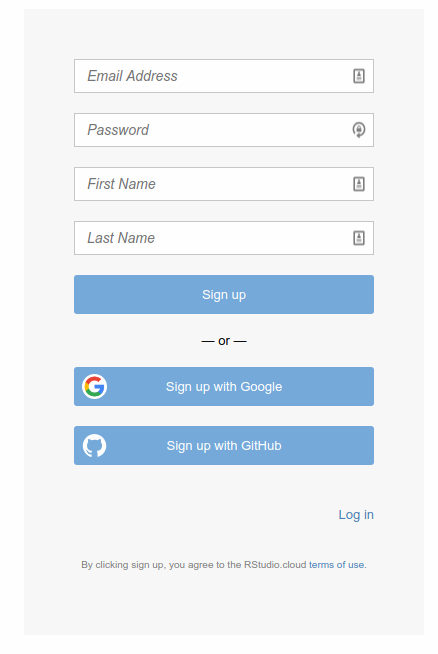
\includegraphics{Screenshot_2018-07-02_14-44-18.png}

If you're happy with using your Google account, click that button. You
will probably have to enter your Google password. (If you are doing this
on your own computer, you might not have to do that.) If you have a
GitHub account and you want to use \emph{that}, same principle. You can
also use an email address as your login to R Studio Cloud. (You can use
any e-mail address; I'm not checking.) Enter it in the top box, and
enter a password to use with R Studio Cloud in the second. (This does
not have to be, and indeed probably should not be, the same as your
email password.) Below that, enter your first and last name. This will
appear at the top right of the screen when you are logged in. Then click
Sign Up. After that, you will have to make a unique account name (which
\emph{you} actually never use, but which \texttt{rstudio.cloud} uses to
name your files). After that, you are automatically logged in.

\begin{enumerate}
\def\labelenumi{(\alph{enumi})}
\setcounter{enumi}{2}
\tightlist
\item
  Take a look around, and create a new Project. Give the new project any
  name you like.
\end{enumerate}

Solution

This is what you see now:

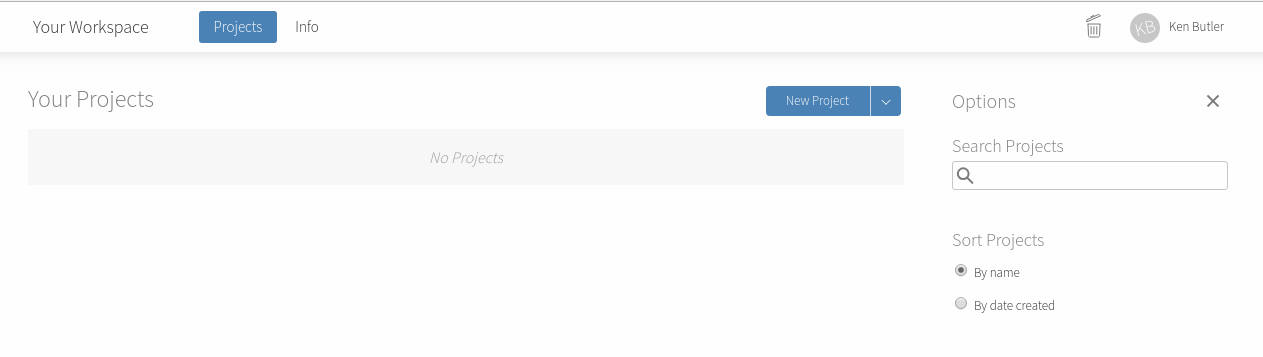
\includegraphics{Screenshot_2018-07-02_15-08-07.png}

Click on the blue New Project button to create a new Project. (A project
is a self-contained piece of work, like for example an assignment.) You
will see the words ``Loading Project'' and spinning circles for a few
moments. Then you see this:

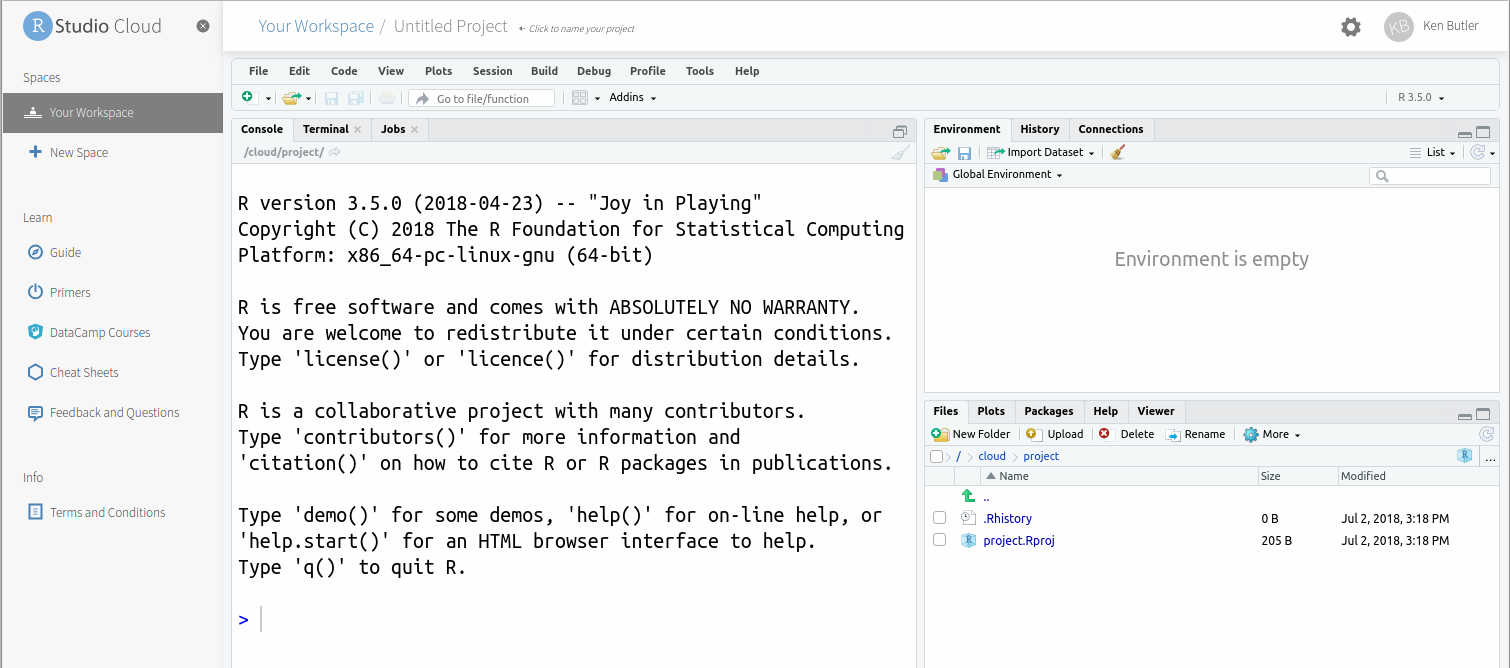
\includegraphics{Screenshot_2018-07-02_15-19-12.png}

To give your project a name, click at the top where it says Untitled
Project and type a name like Assignment 0 into the box.

\begin{enumerate}
\def\labelenumi{(\alph{enumi})}
\setcounter{enumi}{3}
\tightlist
\item
  Before we get to work, look for the blue \texttt{\textgreater{}} at
  the bottom left. Click next to it to get a flashing cursor, and then
  type what you see here (in blue):
\end{enumerate}

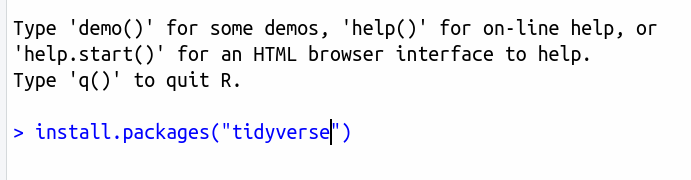
\includegraphics{Screenshot_2018-07-02_15-25-20.png}

Then press Enter.

Solution

This lets it install a bunch of things. It may take some time. If you
are watching it, look out for lines beginning with \texttt{g++}, which
are C++ code that needs to be compiled. This is the end of what I had.
Look out for the word DONE near the bottom:

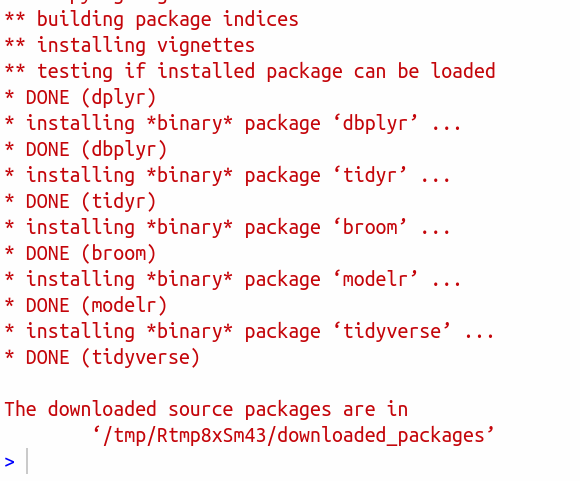
\includegraphics{Screenshot_2018-07-02_15-34-40.png}

\begin{enumerate}
\def\labelenumi{(\alph{enumi})}
\setcounter{enumi}{4}
\tightlist
\item
  Not for now, but for later: if you are on a lab computer, you should
  probably log out when you are done. To do that, find your name at the
  top right. Click on it, and two things should pop out to the right:
  Profile and Log Out. Select Log Out. You should be returned to one of
  the screens you began with, possibly the Welcome to R Studio Cloud
  one. To log back in, now or next time, look for Log In at the top
  right. Click it, to get this:
\end{enumerate}

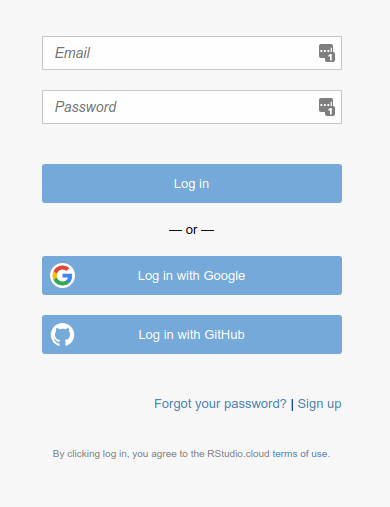
\includegraphics{Screenshot_2018-07-02_15-54-17.png}

and then you can log in with your email and password, or Google or
Github IDs, whichever you used. Now we can get down to some actual work.

\hypertarget{getting-started}{%
\section{Getting started}\label{getting-started}}

This question is to get you started using R.

\begin{enumerate}
\def\labelenumi{(\alph{enumi})}
\tightlist
\item
  Start R Studio Cloud, in some project. (If you started up a new
  project in the previous question and are still logged in, use that; if
  not, create a new project.)
\end{enumerate}

Solution

You ought to see something like this. I have a dark blue background
here, which you probably do not.

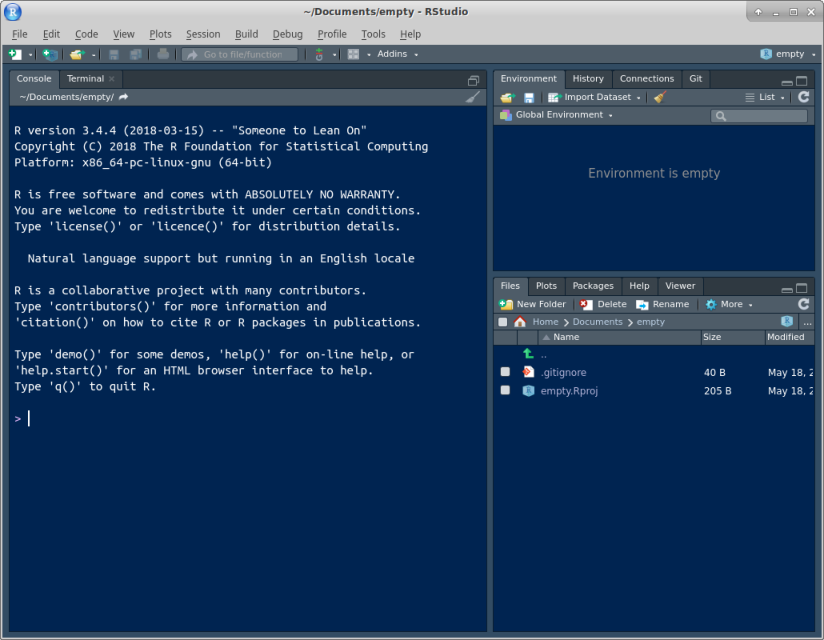
\includegraphics{empty.png}

It won't look exactly like that (for example, the background will
probably be white) but there should be one thing on the left half, and
at the top right it'll say ``Environment is empty''. Extra: if you want
to tweak things, select Tools (at the top of the screen) and from it
Global Options, then click Appearance. You can make the text bigger or
smaller via Editor Font Size, and choose a different colour scheme by
picking one of the Editor Themes (which previews on the right). My
favourite is Tomorrow Night Blue. Click Apply or OK when you have found
something you like. (I spend a lot of time in R Studio, and I like
having a dark background to be easier on my eyes.)

\begin{enumerate}
\def\labelenumi{(\alph{enumi})}
\setcounter{enumi}{1}
\tightlist
\item
  We're going to do some stuff in R here, just to get used to it. First,
  make an R Notebook by selecting File, New File and R Notebook.
\end{enumerate}

Solution

The first time, you'll be invited to ``install some packages'' to make
the Notebook thing work. Let it do that by clicking Yes. After that,
you'll have this:

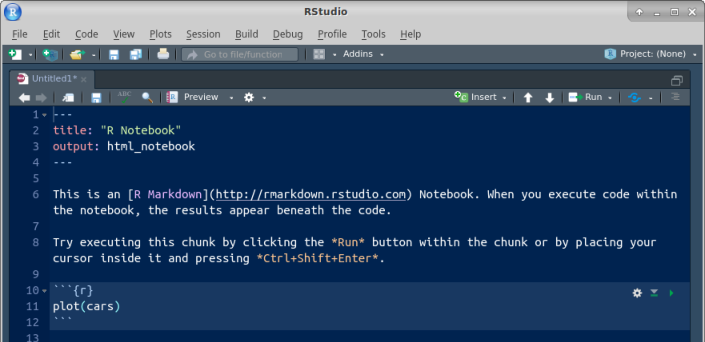
\includegraphics{rnote1.png}

Find the Insert and Run buttons along the top of the R Notebook window.
We'll be using them shortly. (The template notebook may or may not be
maximized; it doesn't matter either way. You might see all four panes or
as few as one. If you want to control that, select View at the top, then
Panes, then either Show All Panes or Zoom Source, as you prefer. In the
menus, you'll also see keyboard shortcuts for these, which you might
find worth learning.)

\begin{enumerate}
\def\labelenumi{(\alph{enumi})}
\setcounter{enumi}{2}
\tightlist
\item
  Change the title to something of your choosing. Then go down to line
  5, click on the Insert button and select R. You should see a ``code
  chunk'' appear at line 5, which we are going to use in a moment.
\end{enumerate}

Solution

Something like this:

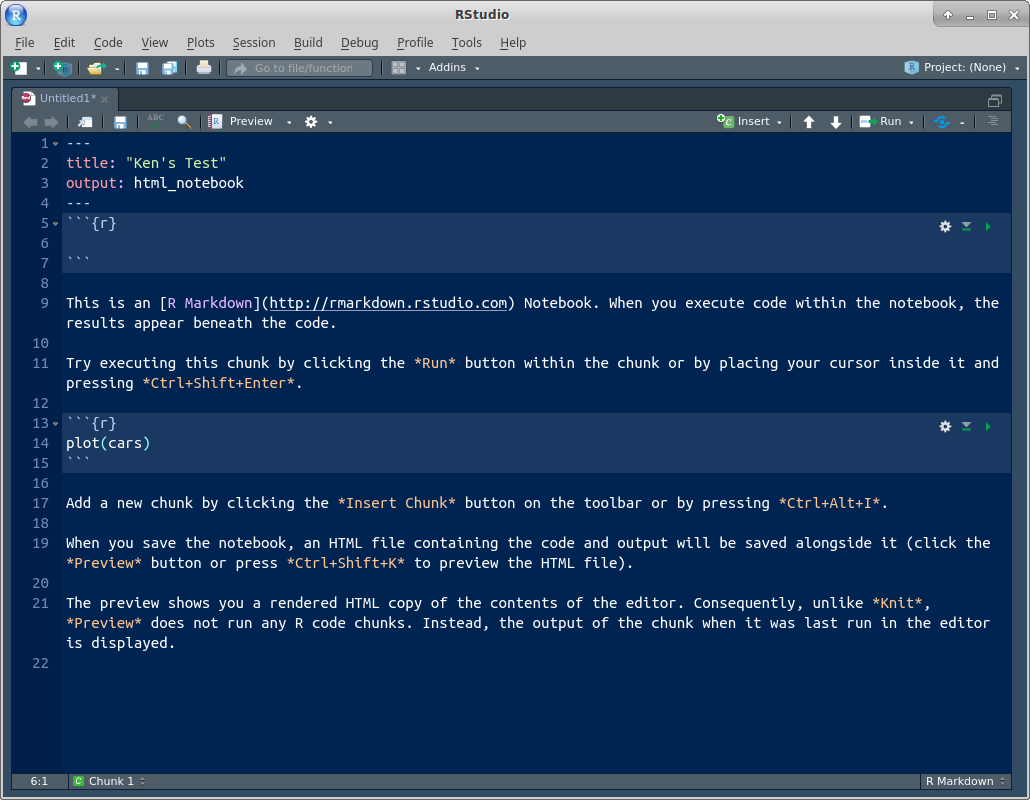
\includegraphics{chunk1.png}

\begin{enumerate}
\def\labelenumi{(\alph{enumi})}
\setcounter{enumi}{3}
\tightlist
\item
  Type the line of code shown below into the chunk in the R Notebook:
\end{enumerate}

\begin{verbatim}

mtcars
\end{verbatim}

Solution

What this will do: get hold of a built-in data set with information
about some different models of car, and display it.

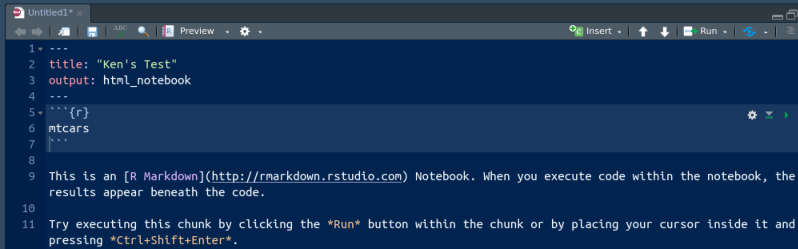
\includegraphics{chunk2.png}

In approximately five seconds, you'll be demonstrating that for
yourself.

\begin{enumerate}
\def\labelenumi{(\alph{enumi})}
\setcounter{enumi}{4}
\tightlist
\item
  Run this command. To do that, look at the top right of your code chunk
  block (shaded in a slightly different colour). You should see a gear
  symbol, a down arrow and a green ``play button''. Click the play
  button. This will run the code, and show the output below the code
  chunk.
\end{enumerate}

Solution

Here's what I get (yours will be the same).

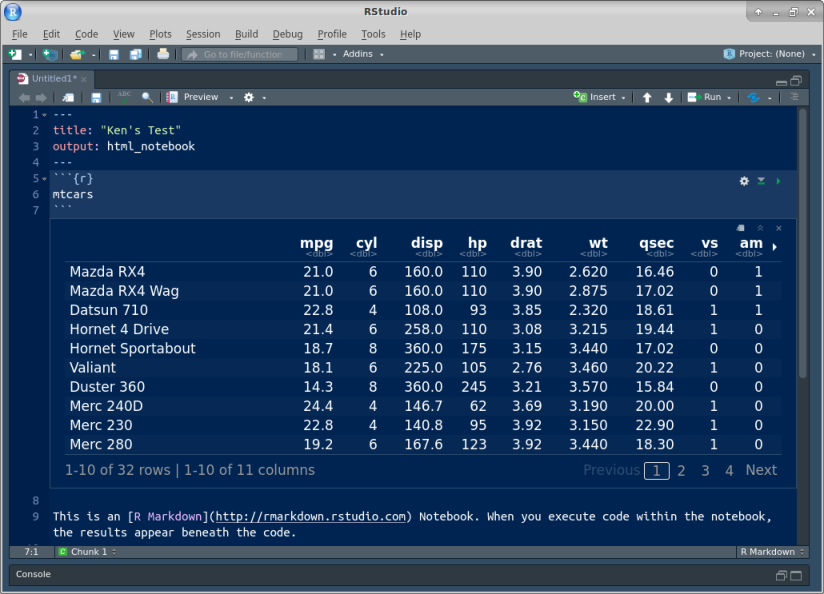
\includegraphics{chunk3.png}

This is a rectangular array of rows and columns, with individuals in
rows and variables in columns, known as a ``data frame''. When you
display a data frame in an R Notebook, you see 10 rows and as many
columns as will fit on the screen. At the bottom, it says how many rows
and columns there are altogether (here 32 rows and 11 columns), and
which ones are being displayed. You can see more rows by clicking on
Next, and if there are more columns, you'll see a little arrow next to
the rightmost column (as here next to \texttt{am}) that you can click on
to see more columns. Try it and see. Or if you want to go to a
particular collection of rows, click one of the numbers between Previous
and Next: 1 is rows 1--10, 2 is rows 11--20, and so on. The column on
the left without a header (containing the names of the cars) is called
``row names''. These have a funny kind of status, kind of a column and
kind of not a column; usually, if we need to use the names, we have to
put them in a column first. In future solutions, rather than showing you
a screenshot, expect me to show you something like this:

\begin{Shaded}
\begin{Highlighting}[]
\NormalTok{mtcars}
\end{Highlighting}
\end{Shaded}

\begin{verbatim}
## # A tibble: 32 x 11
##      mpg   cyl  disp    hp  drat    wt  qsec
##  * <dbl> <dbl> <dbl> <dbl> <dbl> <dbl> <dbl>
##  1  21       6  160    110  3.9   2.62  16.5
##  2  21       6  160    110  3.9   2.88  17.0
##  3  22.8     4  108     93  3.85  2.32  18.6
##  4  21.4     6  258    110  3.08  3.22  19.4
##  5  18.7     8  360    175  3.15  3.44  17.0
##  6  18.1     6  225    105  2.76  3.46  20.2
##  7  14.3     8  360    245  3.21  3.57  15.8
##  8  24.4     4  147.    62  3.69  3.19  20  
##  9  22.8     4  141.    95  3.92  3.15  22.9
## 10  19.2     6  168.   123  3.92  3.44  18.3
## # ... with 22 more rows, and 4 more
## #   variables: vs <dbl>, am <dbl>,
## #   gear <dbl>, carb <dbl>
\end{verbatim}

The top bit is the code, the bottom bit with the \texttt{\#\#} the
output. In this kind of display, you only see the first ten rows (by
default).

If you don't see the ``play button'', make sure that what you have
really is a code chunk. (I often accidentally delete one of the special
characters above or below the code chunk). If you can't figure it out,
delete this code chunk and make a new one. Sometimes R Studio gets
confused.

On the code chunk, the other symbols are the settings for this chunk
(you have the choice to display or not display the code or the output or
to not actually run the code). The second one, the down arrow, runs all
the chunks prior to this one (but not this one).

The output has its own little buttons. The first one pops the output out
into its own window; the second one shows or hides the output, and the
third one deletes the output (so that you have to run the chunk again to
get it back). Experiment. You can't do much damage here.

\begin{enumerate}
\def\labelenumi{(\alph{enumi})}
\setcounter{enumi}{5}
\tightlist
\item
  Something a little more interesting: \texttt{summary} obtains a
  summary of whatever you feed it (the five-number summary plus the mean
  for numerical variables). Obtain this for our data frame. To do this,
  create a new code chunk below the previous one, type
  \texttt{summary(mtcars)} into the code chunk, and run it.
\end{enumerate}

Solution

This is what you should see:

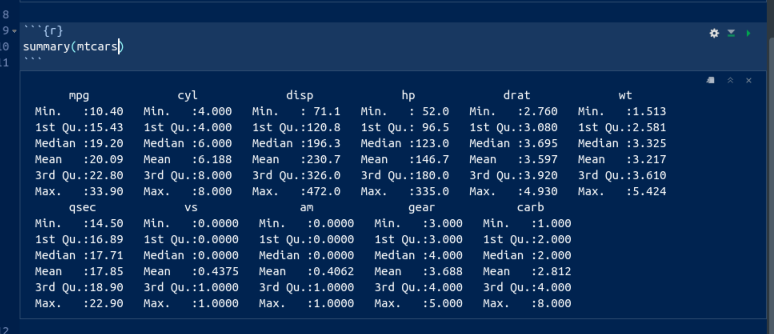
\includegraphics{chunk4.png}

or the other way:

\begin{Shaded}
\begin{Highlighting}[]
\KeywordTok{summary}\NormalTok{(mtcars)}
\end{Highlighting}
\end{Shaded}

\begin{verbatim}
##       mpg             cyl       
##  Min.   :10.40   Min.   :4.000  
##  1st Qu.:15.43   1st Qu.:4.000  
##  Median :19.20   Median :6.000  
##  Mean   :20.09   Mean   :6.188  
##  3rd Qu.:22.80   3rd Qu.:8.000  
##  Max.   :33.90   Max.   :8.000  
##       disp             hp       
##  Min.   : 71.1   Min.   : 52.0  
##  1st Qu.:120.8   1st Qu.: 96.5  
##  Median :196.3   Median :123.0  
##  Mean   :230.7   Mean   :146.7  
##  3rd Qu.:326.0   3rd Qu.:180.0  
##  Max.   :472.0   Max.   :335.0  
##       drat             wt       
##  Min.   :2.760   Min.   :1.513  
##  1st Qu.:3.080   1st Qu.:2.581  
##  Median :3.695   Median :3.325  
##  Mean   :3.597   Mean   :3.217  
##  3rd Qu.:3.920   3rd Qu.:3.610  
##  Max.   :4.930   Max.   :5.424  
##       qsec             vs        
##  Min.   :14.50   Min.   :0.0000  
##  1st Qu.:16.89   1st Qu.:0.0000  
##  Median :17.71   Median :0.0000  
##  Mean   :17.85   Mean   :0.4375  
##  3rd Qu.:18.90   3rd Qu.:1.0000  
##  Max.   :22.90   Max.   :1.0000  
##        am              gear      
##  Min.   :0.0000   Min.   :3.000  
##  1st Qu.:0.0000   1st Qu.:3.000  
##  Median :0.0000   Median :4.000  
##  Mean   :0.4062   Mean   :3.688  
##  3rd Qu.:1.0000   3rd Qu.:4.000  
##  Max.   :1.0000   Max.   :5.000  
##       carb      
##  Min.   :1.000  
##  1st Qu.:2.000  
##  Median :2.000  
##  Mean   :2.812  
##  3rd Qu.:4.000  
##  Max.   :8.000
\end{verbatim}

For the gas mileage column \texttt{mpg}, the mean is bigger than the
median, and the largest value is unusually large compared with the
others, suggesting a distribution that is skewed to the right.

There are 11 numeric (quantitative) variables, so we get the five-number
summary plus mean for each one. Categorical variables, if we had any
here, would be displayed a different way.

(In case you are wondering, the way without screenshots is obtained by
\emph{my} writing a notebook with code chunks and running them, so this
output genuinely \emph{is} obtained by running the code you see.)

\begin{enumerate}
\def\labelenumi{(\alph{enumi})}
\setcounter{enumi}{6}
\tightlist
\item
  Let's make a boxplot of the gas mileage data. This is a ``poor man's
  boxplot''; we'll see a nicer-looking way later. To do it this way,
  make another new code chunk, enter the code
  \texttt{boxplot(mtcars\$mpg)} into it, and run the chunk.
\end{enumerate}

Solution

This is what you should see:

\begin{Shaded}
\begin{Highlighting}[]
\KeywordTok{boxplot}\NormalTok{(mtcars}\OperatorTok{$}\NormalTok{mpg)}
\end{Highlighting}
\end{Shaded}

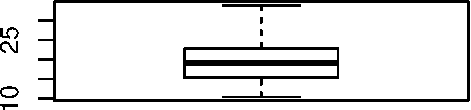
\includegraphics{01-getting-used_files/figure-latex/unnamed-chunk-8-1}

The long upper whisker supports our guess from before that the
distribution is right-skewed.

\begin{enumerate}
\def\labelenumi{(\alph{enumi})}
\setcounter{enumi}{7}
\tightlist
\item
  Some aesthetics to finish with: delete the template notebook (all the
  stuff you didn't type below your code chunks and output). Then add
  some narrative text above and below your code chunks. Above the code
  chunk is where you say what you are going to do (and maybe why you are
  doing it), and below is where you say what you conclude from the
  output you just obtained.
\end{enumerate}

Solution

My complete R Notebook is at
\url{http://www.utsc.utoronto.ca/~butler/c32/a0-notebook-1.Rmd}. Take a
look at it. I added one extra thing: my variable names have
``backticks'' around them. You'll see the effect of this in a moment.
Backtick is on the key to the left of 1 and below Esc on your keyboard,
along with a ``squiggle'' symbol that we'll be using later in the
course.

\begin{enumerate}
\def\labelenumi{(\roman{enumi})}
\tightlist
\item
  Save your notebook (the usual way with File and Save). This saves it
  \emph{on the R Studio Cloud servers} (and not on your computer). This
  means that when you come back to R Studio Cloud later, even from
  another device, this notebook will still be available to you. Now
  click Preview. This produces a pretty HTML version of your notebook.
\end{enumerate}

Solution

Note that the HTML document only contains output from the chunks you've
run in the notebook, so it's up to you to run them there first.\\
My HTML document is at
\url{http://www.utsc.utoronto.ca/~butler/c32/a0-notebook-1.nb.html}.
Here's where you see the effect of the backticks: all the variable names
are in \texttt{typewriter\ font} so that you can see they are variable
names and not something else. If you want to try this notebook out
yourself, you have a couple of options: (i) make a new R Notebook on R
Studio Cloud and copy-paste the contents of my file (it's just text), or
(ii) download my R Notebook onto your computer, and then upload it to R
Studio Cloud. Look in the Files pane bottom right, and next to New
Folder you should see Upload. Upload the file from wherever it got saved
to when you downloaded it. Extra: if you're feeling ambitious, click the
arrow to the right of Preview and select Knit to Word. The button
changes to Knit with a ball of wool beside it. Now, when you ``knit''
the notebook, you get a Word document directly --- look for it in the
Files pane. If you want to, you can hand this kind of thing in (on later
assignments), but you'll have to do a little work first: first, find it
in your Files list, then click the checkbox to the left of it, then
click More (with the gear, on the same line as New Folder and Upload),
then select Export (and click Download). This will put a copy in your
downloads folder on your computer, and you can open it from there. If
you're feeling extra-ambitious, you can try Knit to PDF. This produces
something that looks as if it was written in LaTeX, but actually wasn't.
To make this work, if you have a \texttt{library(tidyverse)} line
somewhere, as you probably will, find the code chunk it's in, and make
it look like this:

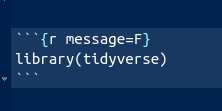
\includegraphics{Screenshot_2018-10-10_17-24-47.png}

Then it will work. Extra extra: if you like the keyboard better than the
mouse, R Studio has a lot of keyboard shortcuts. Two that are useful
now: control-alt-i inserts a code chunk where the cursor is, and
control-shift-enter runs the code chunk that the cursor is in, if it is
in one. (Mac users, ``command'' instead of ``control'' in both cases.) I
use these two a lot.

\begin{enumerate}
\def\labelenumi{(\alph{enumi})}
\setcounter{enumi}{9}
\tightlist
\item
  Optional extra: practice handing in your previewed R notebook, as if
  it were an assignment that was worth something. (It is good to get the
  practice in a low-stakes situation, so that you'll know what to do
  next week.)
\end{enumerate}

Solution

There are two steps: download the HTML file onto your computer, and then
handing it in on Quercus. To download: find the HTML file that you want
to download in the Files pane bottom right. There should be two files
starting with the same thing, eg. \texttt{test1.Rmd}, which is the
notebook you wrote, and \texttt{test1.nb.html}, which is the previewed
version of it, and is the one you want to download. (The \texttt{test1}
part is the name \emph{you} chose when you saved it.) Click the checkbox
to the left of the HTML file. Now click on More above the bottom-right
pane. This pops up a menu from which you choose Export. This will pop up
another window called Export Files, where you put the name that the file
will have on your computer. (I usually leave the name the same.) Click
Download. The file will go to your Downloads folder, or wherever things
you download off the web go. Now, to hand it in. Open up Quercus at
\texttt{q.utoronto.ca}, log in and navigate to this course. Click
Assignments. Click (the title of) Assignment 0. There is a big blue
Submit Assignment button top right. Click it. You'll get a File Upload
at the bottom of the screen. Click Choose File and find the HTML file
that you downloaded. Click Open (or equivalent on your system). The name
of the file should appear next to Choose File. Click Submit Assignment.
You'll see Submitted at the top right. If you want to try this again,
you can Re-submit Assignment as many times as you like. (For the real
thing, you can use this if you realize you made a mistake in something
you submitted. The graders' instructions, for the real thing, are to
grade the \emph{last} file submitted, so in that case you need to make
sure that the last thing submitted includes \emph{everything} that you
want graded. Here, though, it doesn't matter.)

\begin{enumerate}
\def\labelenumi{(\alph{enumi})}
\setcounter{enumi}{10}
\tightlist
\item
  Optional extra. Something more ambitious: make a scatterplot of gas
  mileage \texttt{mpg}, on the \(y\) axis, against horsepower,
  \texttt{hp}, on the \(x\)-axis.
\end{enumerate}

Solution

That goes like this. I'll explain the steps below.

\begin{Shaded}
\begin{Highlighting}[]
\KeywordTok{library}\NormalTok{(tidyverse)}
\KeywordTok{ggplot}\NormalTok{(mtcars, }\KeywordTok{aes}\NormalTok{(}\DataTypeTok{x =}\NormalTok{ hp, }\DataTypeTok{y =}\NormalTok{ mpg)) }\OperatorTok{+}\StringTok{ }\KeywordTok{geom_point}\NormalTok{()}
\end{Highlighting}
\end{Shaded}

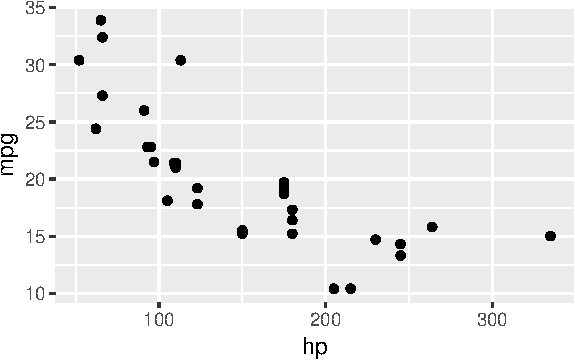
\includegraphics{01-getting-used_files/figure-latex/unnamed-chunk-9-1}
\$ \%\$ \%\$

This shows a somewhat downward trend, which is what you'd expect, since
a larger \texttt{hp} value means a more powerful engine, which will
probably consume more gas and get \emph{fewer} miles per gallon. As for
the code: to make a \texttt{ggplot} plot, as we will shortly see in
class, you first need a \texttt{ggplot} statement that says what to
plot. The first thing in a \texttt{ggplot} is a data frame
(\texttt{mtcars} here), and then the \texttt{aes} says that the plot
will have \texttt{hp} on the \(x\)-axis and \texttt{mpg} on the
\(y\)-axis, taken from the data frame that you specified. That's all of
the what-to-plot. The last thing is how to plot it;
\texttt{geom\_point()} says to plot the data values as points.

You might like to add a regression line to the plot. That is a matter of
adding this to the end of the plotting command:

\begin{Shaded}
\begin{Highlighting}[]
\KeywordTok{ggplot}\NormalTok{(mtcars, }\KeywordTok{aes}\NormalTok{(}\DataTypeTok{x =}\NormalTok{ hp, }\DataTypeTok{y =}\NormalTok{ mpg)) }\OperatorTok{+}\StringTok{ }\KeywordTok{geom_point}\NormalTok{() }\OperatorTok{+}\StringTok{ }
\StringTok{    }\KeywordTok{geom_smooth}\NormalTok{(}\DataTypeTok{method =} \StringTok{"lm"}\NormalTok{)}
\end{Highlighting}
\end{Shaded}

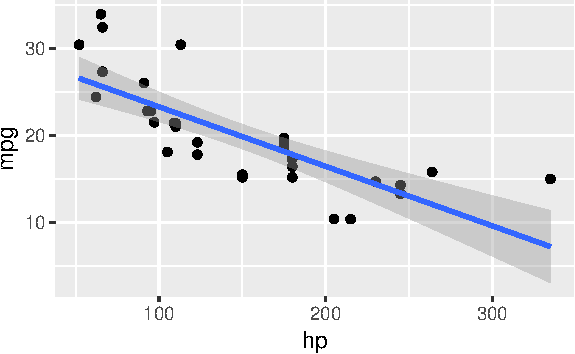
\includegraphics{01-getting-used_files/figure-latex/unnamed-chunk-10-1}

The line definitely goes downhill. Decide for yourself how well you
think a line fits these data.

\hypertarget{reading-data-from-a-file}{%
\section{Reading data from a file}\label{reading-data-from-a-file}}

In this question, we read a file from the web and do some descriptive
statistics and a graph. This is very like what you will be doing on
future assignments, so it's good to practice it now.

Take a look at the data file at
\url{https://www.utsc.utoronto.ca/~butler/c32/jumping.txt}. These are
measurements on 30 rats that were randomly made to do different amounts
of jumping by group (we'll see the details later in the course). The
control group did no jumping, and the other groups did ``low jumping''
and ``high jumping''. The first column says which jumping group each rat
was in, and the second is the rat's bone density (the experimenters'
supposition was that more jumping should go with higher bone density).

\begin{enumerate}
\def\labelenumi{(\alph{enumi})}
\tightlist
\item
  What are the two columns of data separated by? (The fancy word is
  ``delimited'').
\end{enumerate}

Solution

Exactly one space. This is true all the way down, as you can check.

\begin{enumerate}
\def\labelenumi{(\alph{enumi})}
\setcounter{enumi}{1}
\tightlist
\item
  Make a new R Notebook. Leave the first four lines, but get rid of the
  rest of the template document. Start with a code chunk containing
  \texttt{library(tidyverse)}. Run it.
\end{enumerate}

Solution

You will get either the same message as before or nothing. (I got
nothing because I had already loaded the \texttt{tidyverse} in this
session.)

\begin{enumerate}
\def\labelenumi{(\alph{enumi})}
\setcounter{enumi}{2}
\tightlist
\item
  Put the URL of the data file in a variable called \texttt{my\_url}.
  Then use \texttt{read\_delim} to read in the file. (See solutions for
  how.) \texttt{read\_delim} reads data files where the data values are
  always separated by the same single character, here a space. Save the
  data frame in a variable \texttt{rats}.
\end{enumerate}

Solution

Like this:

\begin{Shaded}
\begin{Highlighting}[]
\NormalTok{my_url =}\StringTok{ "https://www.utsc.utoronto.ca/~butler/c32/jumping.txt"}
\NormalTok{rats =}\StringTok{ }\KeywordTok{read_delim}\NormalTok{(my_url, }\StringTok{" "}\NormalTok{)}
\end{Highlighting}
\end{Shaded}

\begin{verbatim}
## Parsed with column specification:
## cols(
##   group = col_character(),
##   density = col_integer()
## )
\end{verbatim}

The second thing in \texttt{read\_delim} is the thing that separates the
data values. Often when you use \texttt{read\_delim} it'll be a space.

\begin{enumerate}
\def\labelenumi{(\alph{enumi})}
\setcounter{enumi}{3}
\tightlist
\item
  Take a look at your data frame, by making a new code chunk and putting
  the data frame's name in it (as we did with \texttt{mtcars}).
\end{enumerate}

Solution

\begin{Shaded}
\begin{Highlighting}[]
\NormalTok{rats}
\end{Highlighting}
\end{Shaded}

\begin{verbatim}
## # A tibble: 30 x 2
##    group   density
##    <chr>     <int>
##  1 Control     611
##  2 Control     621
##  3 Control     614
##  4 Control     593
##  5 Control     593
##  6 Control     653
##  7 Control     600
##  8 Control     554
##  9 Control     603
## 10 Control     569
## # ... with 20 more rows
\end{verbatim}

There are 30 rows and two columns, as there should be.

\begin{enumerate}
\def\labelenumi{(\alph{enumi})}
\setcounter{enumi}{4}
\tightlist
\item
  Find the mean bone density for rats that did each amount of jumping.
\end{enumerate}

Solution

This is something you'll see a lot: \texttt{group\_by} followed by
\texttt{summarize}. Reminder: to get that funny thing with the percent
signs (called the ``pipe symbol''), type control-shift-M (or equivalent
on a Mac):

\begin{Shaded}
\begin{Highlighting}[]
\NormalTok{rats }\OperatorTok\StringTok{ }\KeywordTok{group_by}\NormalTok{(group) }\OperatorTok\StringTok{ }\KeywordTok{summarize}\NormalTok{(}\DataTypeTok{m =} \KeywordTok{mean}\NormalTok{(density))}
\end{Highlighting}
\end{Shaded}

\begin{verbatim}
## # A tibble: 3 x 2
##   group        m
##   <chr>    <dbl>
## 1 Control   601.
## 2 Highjump  639.
## 3 Lowjump   612.
\end{verbatim}

The mean bone density is clearly highest for the high jumping group, and
not much different between the low-jumping and control groups.

\begin{enumerate}
\def\labelenumi{(\alph{enumi})}
\setcounter{enumi}{5}
\tightlist
\item
  Make a boxplot of bone density for each jumping group.
\end{enumerate}

Solution

On a boxplot, the groups go across and the values go up and down, so the
right syntax is this:

\begin{Shaded}
\begin{Highlighting}[]
\KeywordTok{ggplot}\NormalTok{(rats, }\KeywordTok{aes}\NormalTok{(}\DataTypeTok{x =}\NormalTok{ group, }\DataTypeTok{y =}\NormalTok{ density)) }\OperatorTok{+}\StringTok{ }\KeywordTok{geom_boxplot}\NormalTok{()}
\end{Highlighting}
\end{Shaded}

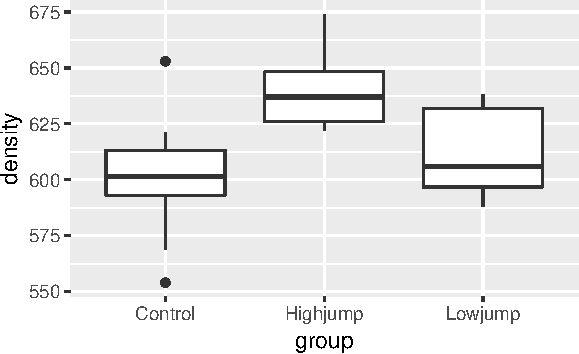
\includegraphics{01-getting-used_files/figure-latex/unnamed-chunk-14-1}

Given the amount of variability, the control and low-jump groups are
very similar (with the control group having a couple of outliers), but
the high-jump group seems to have a consistently higher bone density
than the others.

This is more or less in line with what the experimenters were guessing,
but it seems that it has to be high jumping to make a difference.

You might recognize that this is the kind of data where we would use
analysis of variance, which we will do later on in the course: we are
comparing several (here three) groups.

\hypertarget{reading-in-data-and-drawing-some-graphs}{%
\chapter{Reading in data and drawing some
graphs}\label{reading-in-data-and-drawing-some-graphs}}

\hypertarget{orange-juice}{%
\section{Orange juice}\label{orange-juice}}

The quality of orange juice produced by a manufacturer (identity
unknown) is constantly being monitored. The manufacturer has developed a
``sweetness index'' for its orange juice, for which a higher value means
sweeter juice. Is the sweetness index related to a chemical measure such
as the amount of water-soluble pectin (parts per million) in the orange
juice? Data were obtained from 24 production runs, and the sweetness and
pectin content were measured for each run. The data are in
\href{http://www.utsc.utoronto.ca/~butler/c32/ojuice.txt}{link}. Open
that link up now. You can click on that link just above to open the
file.

\begin{enumerate}
\def\labelenumi{(\alph{enumi})}
\tightlist
\item
  The data values are separated by a space. Use the appropriate
  Tidyverse function to read the data directly from the course website
  into a ``tibble''.
\end{enumerate}

Solution

Start with this (almost always):

\begin{Shaded}
\begin{Highlighting}[]
\KeywordTok{library}\NormalTok{(tidyverse)}
\end{Highlighting}
\end{Shaded}

\begin{verbatim}
## -- Attaching packages ---- tidyverse 1.2.1 --
\end{verbatim}

\begin{verbatim}
## v ggplot2 3.1.0     v purrr   0.2.5
## v tibble  1.4.2     v dplyr   0.7.8
## v tidyr   0.8.1     v stringr 1.3.1
## v readr   1.1.1     v forcats 0.3.0
\end{verbatim}

\begin{verbatim}
## -- Conflicts ------- tidyverse_conflicts() --
## x dplyr::filter() masks stats::filter()
## x dplyr::lag()    masks stats::lag()
\end{verbatim}

The appropriate function, the data values being separated by a space,
will be \texttt{read\_delim}. Put the URL as the first thing in
\texttt{read\_delim}, or (better) define it into a variable first:
\marginnote{I say *better* because otherwise the read line gets rather long. This way you read it as *the URL is some long thing that I don't care about especially, and I what I need to do is to read the data from that URL, separated by spaces.*}

\begin{Shaded}
\begin{Highlighting}[]
\NormalTok{url =}\StringTok{ "http://www.utsc.utoronto.ca/~butler/c32/ojuice.txt"}
\NormalTok{juice =}\StringTok{ }\KeywordTok{read_delim}\NormalTok{(url, }\StringTok{" "}\NormalTok{)}
\end{Highlighting}
\end{Shaded}

\begin{verbatim}
## Parsed with column specification:
## cols(
##   run = col_integer(),
##   sweetness = col_double(),
##   pectin = col_integer()
## )
\end{verbatim}

\texttt{read\_delim} (or \texttt{read\_csv} or any of the others) tell
you what variables were read in, and also tell you about any ``parsing
errors'' where it couldn't work out what was what. Here, we have three
variables, which is entirely consistent with the three columns of data
values in the file.

\texttt{read\_delim} can handle data values separated by \emph{any}
character, not just spaces, but the separating character, known as a
``delimiter'', does \emph{not} have a default, so you have to say what
it is, every time.

\begin{enumerate}
\def\labelenumi{(\alph{enumi})}
\setcounter{enumi}{1}
\tightlist
\item
  Take a look at what got read in. Do you have data for all 24 runs?
\end{enumerate}

Solution

Type the name of the data frame in a code chunk (a new one, or add it to
the end of the previous one). Because this is actually a ``tibble'',
which is what \texttt{read\_delim} reads in, you'll only actually see
the first 10 lines, but it will tell you how many lines there are
altogether, and you can click on the appropriate thing to see the rest
of it.

\begin{Shaded}
\begin{Highlighting}[]
\NormalTok{juice}
\end{Highlighting}
\end{Shaded}

\begin{verbatim}
## # A tibble: 24 x 3
##      run sweetness pectin
##    <int>     <dbl>  <int>
##  1     1       5.2    220
##  2     2       5.5    227
##  3     3       6      259
##  4     4       5.9    210
##  5     5       5.8    224
##  6     6       6      215
##  7     7       5.8    231
##  8     8       5.6    268
##  9     9       5.6    239
## 10    10       5.9    212
## # ... with 14 more rows
\end{verbatim}

I appear to have all the data. If you want further convincing, click
Next a couple of times (on yours) to be sure that the runs go down to
number 24.

\begin{enumerate}
\def\labelenumi{(\alph{enumi})}
\setcounter{enumi}{2}
\tightlist
\item
  In your data frame, where did the column (variable) names come from?
  How did R know where to get them from?
\end{enumerate}

Solution

They came from the top line of the data file, so we didn't have to
specify them. This is the default behaviour of all the \texttt{read\_}
functions, so we don't have to ask for it specially. In fact, if the top
line of your data file is \emph{not} variable names, \emph{that's} when
you have to say something special. The \texttt{read\_} functions have an
option \texttt{col\_names} which can either be \texttt{TRUE} (the
default), which means ``read them in from the top line'', \texttt{FALSE}
(``they are not there, so make some up'') or a list of column names to
use. You might use the last alternative when the column names that are
in the file are \emph{not} the ones you want to use; in that case, you
would also say \texttt{skip=1} to skip the first line. For example, with
file \texttt{a.txt} thus: \texttt{timinput\{}.txt\}\\
you could read the same data but call the columns \texttt{x} and
\texttt{y} thus:

\begin{Shaded}
\begin{Highlighting}[]
\KeywordTok{read_delim}\NormalTok{(}\StringTok{"a.txt"}\NormalTok{, }\StringTok{" "}\NormalTok{, }\DataTypeTok{col_names =} \KeywordTok{c}\NormalTok{(}\StringTok{"x"}\NormalTok{, }\StringTok{"y"}\NormalTok{), }
    \DataTypeTok{skip =} \DecValTok{1}\NormalTok{)}
\end{Highlighting}
\end{Shaded}

\begin{verbatim}
## Parsed with column specification:
## cols(
##   x = col_integer(),
##   y = col_integer()
## )
\end{verbatim}

\begin{verbatim}
## # A tibble: 3 x 2
##       x     y
##   <int> <int>
## 1     1     2
## 2     3     4
## 3     5     6
\end{verbatim}

\begin{enumerate}
\def\labelenumi{(\alph{enumi})}
\setcounter{enumi}{3}
\tightlist
\item
  The juice manufacturer was interested in whether there was a
  relationship between sweetness and pectin. To assess this, draw a
  scatterplot. Does it look as if there is any kind of a relationship?
  (I think \texttt{sweetness} is the outcome variable and
  \texttt{pectin} is explanatory, so draw your scatterplot
  appropriately.)
\end{enumerate}

Solution

This requires a \texttt{ggplot} plot. You can go back and look at the
lecture notes to figure out how to make a scatterplot: the ``what to
plot'' is the \(x\)-axis and \(y\)-axis variables, with the response on
the \(y\)-axis (starting with a data frame to get the variables from),
and the ``how to plot'' is \texttt{geom\_point} to plot the points:

\begin{Shaded}
\begin{Highlighting}[]
\KeywordTok{ggplot}\NormalTok{(juice, }\KeywordTok{aes}\NormalTok{(}\DataTypeTok{x =}\NormalTok{ pectin, }\DataTypeTok{y =}\NormalTok{ sweetness)) }\OperatorTok{+}\StringTok{ }
\StringTok{    }\KeywordTok{geom_point}\NormalTok{()}
\end{Highlighting}
\end{Shaded}

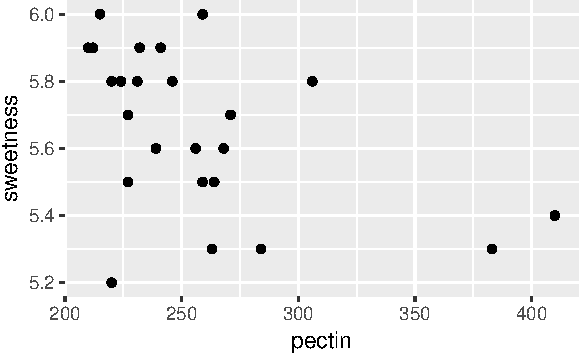
\includegraphics{02-reading-in_files/figure-latex/unnamed-chunk-8-1}

It looks to me as if there is a negative relationship: as pectin goes
up, sweetness tends to go \emph{down}. The trend appears to go top left
to bottom right.

Having said that, I'm wondering how much of the apparent trend is caused
by those two observations bottom right with pectin over 350. If you take
those away, the trend seems to me to be a lot less convincing. As an
extra, you could add a smooth trend to the plot:

\begin{Shaded}
\begin{Highlighting}[]
\KeywordTok{ggplot}\NormalTok{(juice, }\KeywordTok{aes}\NormalTok{(}\DataTypeTok{x =}\NormalTok{ pectin, }\DataTypeTok{y =}\NormalTok{ sweetness)) }\OperatorTok{+}\StringTok{ }
\StringTok{    }\KeywordTok{geom_point}\NormalTok{() }\OperatorTok{+}\StringTok{ }\KeywordTok{geom_smooth}\NormalTok{()}
\end{Highlighting}
\end{Shaded}

\begin{verbatim}
## `geom_smooth()` using method = 'loess' and formula 'y ~ x'
\end{verbatim}

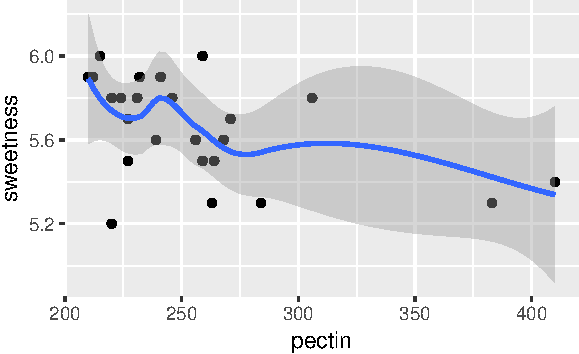
\includegraphics{02-reading-in_files/figure-latex/unnamed-chunk-9-1}

The smooth trend is kind of downhill, but not very convincing.

\hypertarget{making-soap}{%
\section{Making soap}\label{making-soap}}

A company operates two production lines in a factory for making soap
bars. The production lines are labelled A and B. A production line that
moves faster may produce more soap, but may possibly also produce more
``scrap'' (that is, bits of soap that can no longer be made into soap
bars and will have to be thrown away).

The data are in
\href{http://www.utsc.utoronto.ca/~butler/c32/soap.txt}{link}.

\begin{enumerate}
\def\labelenumi{(\alph{enumi})}
\tightlist
\item
  Read the data into R. Display the data. There should be 27 rows. Are
  there?
\end{enumerate}

Solution

Read directly from the URL, most easily:

\begin{Shaded}
\begin{Highlighting}[]
\NormalTok{url =}\StringTok{ "http://www.utsc.utoronto.ca/~butler/c32/soap.txt"}
\NormalTok{soap =}\StringTok{ }\KeywordTok{read_delim}\NormalTok{(url, }\StringTok{" "}\NormalTok{)}
\end{Highlighting}
\end{Shaded}

\begin{verbatim}
## Parsed with column specification:
## cols(
##   case = col_integer(),
##   scrap = col_integer(),
##   speed = col_integer(),
##   line = col_character()
## )
\end{verbatim}

\begin{Shaded}
\begin{Highlighting}[]
\NormalTok{soap}
\end{Highlighting}
\end{Shaded}

\begin{verbatim}
## # A tibble: 27 x 4
##     case scrap speed line 
##    <int> <int> <int> <chr>
##  1     1   218   100 a    
##  2     2   248   125 a    
##  3     3   360   220 a    
##  4     4   351   205 a    
##  5     5   470   300 a    
##  6     6   394   255 a    
##  7     7   332   225 a    
##  8     8   321   175 a    
##  9     9   410   270 a    
## 10    10   260   170 a    
## # ... with 17 more rows
\end{verbatim}

27 rows. \texttt{line}, which is either \texttt{a} or \texttt{b}, was
correctly deduced to be text.

\begin{enumerate}
\def\labelenumi{(\alph{enumi})}
\setcounter{enumi}{1}
\tightlist
\item
  Obtain a histogram of the \texttt{scrap} values, using 10 bins for
  your histogram.
\end{enumerate}

Solution

\begin{Shaded}
\begin{Highlighting}[]
\KeywordTok{ggplot}\NormalTok{(soap, }\KeywordTok{aes}\NormalTok{(}\DataTypeTok{x =}\NormalTok{ scrap)) }\OperatorTok{+}\StringTok{ }\KeywordTok{geom_histogram}\NormalTok{(}\DataTypeTok{bins =} \DecValTok{10}\NormalTok{)}
\end{Highlighting}
\end{Shaded}

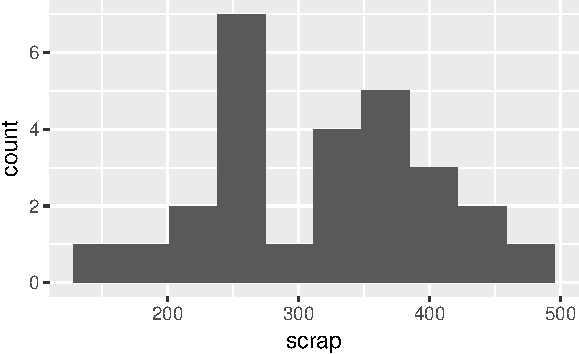
\includegraphics{02-reading-in_files/figure-latex/unnamed-chunk-11-1}

\begin{enumerate}
\def\labelenumi{(\alph{enumi})}
\setcounter{enumi}{2}
\tightlist
\item
  Comment briefly on the shape of the histogram. Is it approximately
  symmetric, skewed to the left, skewed to the right or something else?
  (By ``comment briefly'' I mean ``say in a few words why you gave the
  answer you did.'')
\end{enumerate}

Solution

I would call this ``bimodal''. There are two peaks to the histogram, one
around 250 and one around 370, with a very small frequency in between
(the bar around 300). Apart from the bimodality, there is no particular
evidence for a long tail on either end, so I don't think you could
otherwise call it anything other than symmetric. Having said that (this
is going beyond the question), the way a histogram looks can depend on
the bins you choose to draw it with. This is 8 bins rather than 10:

\begin{Shaded}
\begin{Highlighting}[]
\KeywordTok{ggplot}\NormalTok{(soap, }\KeywordTok{aes}\NormalTok{(}\DataTypeTok{x =}\NormalTok{ scrap)) }\OperatorTok{+}\StringTok{ }\KeywordTok{geom_histogram}\NormalTok{(}\DataTypeTok{bins =} \DecValTok{8}\NormalTok{)}
\end{Highlighting}
\end{Shaded}

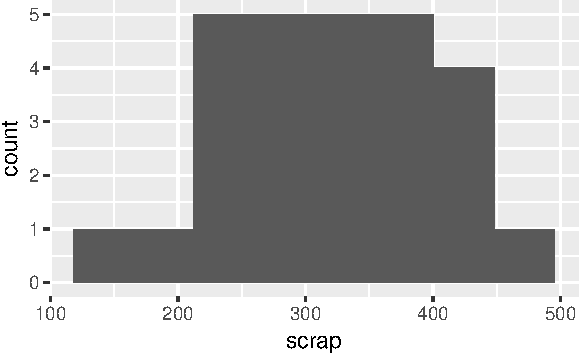
\includegraphics{02-reading-in_files/figure-latex/unnamed-chunk-12-1}

The middle low-frequency bin has gone, and this one just looks
symmetric, with a kind of ``flat top''.

\begin{enumerate}
\def\labelenumi{(\alph{enumi})}
\setcounter{enumi}{3}
\tightlist
\item
  Make side-by-side boxplots of scrap values for each production line.
\end{enumerate}

Solution

\begin{Shaded}
\begin{Highlighting}[]
\KeywordTok{ggplot}\NormalTok{(soap, }\KeywordTok{aes}\NormalTok{(}\DataTypeTok{x =}\NormalTok{ line, }\DataTypeTok{y =}\NormalTok{ scrap)) }\OperatorTok{+}\StringTok{ }\KeywordTok{geom_boxplot}\NormalTok{()}
\end{Highlighting}
\end{Shaded}

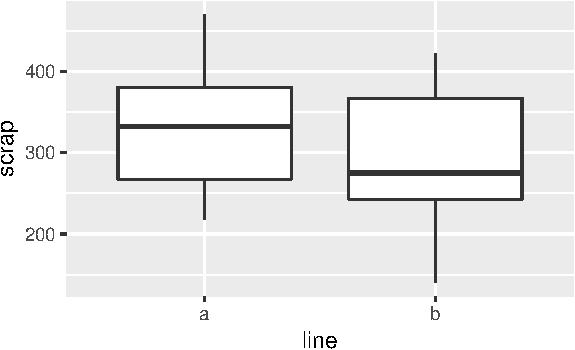
\includegraphics{02-reading-in_files/figure-latex/unnamed-chunk-13-1}

One categorical, one quantitative variable, so boxplots make sense.

\begin{enumerate}
\def\labelenumi{(\alph{enumi})}
\setcounter{enumi}{4}
\tightlist
\item
  Do you think your boxplot says that there are differences in the
  amount of scrap produced by the two production lines, or not? Explain
  briefly.
\end{enumerate}

Solution

I would say that there \emph{is} a difference between the two production
lines, with line A producing an average (median) of about 330 and line B
producing a median of about 275. But you could also make the case that,
although the medians are rather different, there is a lot of variability
and hence a lot of overlap between the two boxplots, and therefore that
there is not a ``substantial'' difference. I would say that either of
those answers are good \emph{if you
back them up with proper reasons}. This is going to be a common theme in
this course: I am going to ask you to make a decision and support it,
where the reasons you provide are often more important than the decision
you make. You might be wondering whether the medians, or means, since
there is no serious skewness here and definitely no outliers, are
``significantly different''. This is inference, which we will come to
later, but a preview looks like this:

\begin{Shaded}
\begin{Highlighting}[]
\KeywordTok{t.test}\NormalTok{(scrap }\OperatorTok{~}\StringTok{ }\NormalTok{line, }\DataTypeTok{data =}\NormalTok{ soap)}
\end{Highlighting}
\end{Shaded}

\begin{verbatim}
## 
##  Welch Two Sample t-test
## 
## data:  scrap by line
## t = 1.2493, df = 21.087, p-value =
## 0.2253
## alternative hypothesis: true difference in means is not equal to 0
## 95 percent confidence interval:
##  -26.97888 108.21222
## sample estimates:
## mean in group a mean in group b 
##        333.5333        292.9167
\end{verbatim}

They are not: the P-value of 0.22 is not anywhere near as small as 0.05,
so we can't reject the null hypothesis that the two lines have equal
mean amount of scrap.

Rusty on this stuff? Don't worry; we're going to come back to it later
in the course.

I was also wondering about something else: that bimodal histogram. Could
that be explained by the scrap values being two different production
lines being mixed together? One way to understand that is to have two
separate histograms, one for each line, side by side, which is what
facetting does. There is an extra wrinkle here that I explain
afterwards:

\begin{Shaded}
\begin{Highlighting}[]
\KeywordTok{ggplot}\NormalTok{(soap, }\KeywordTok{aes}\NormalTok{(}\DataTypeTok{x =}\NormalTok{ scrap)) }\OperatorTok{+}\StringTok{ }\KeywordTok{geom_histogram}\NormalTok{(}\DataTypeTok{bins =} \DecValTok{10}\NormalTok{) }\OperatorTok{+}\StringTok{ }
\StringTok{    }\KeywordTok{facet_grid}\NormalTok{(line }\OperatorTok{~}\StringTok{ }\NormalTok{.)}
\end{Highlighting}
\end{Shaded}

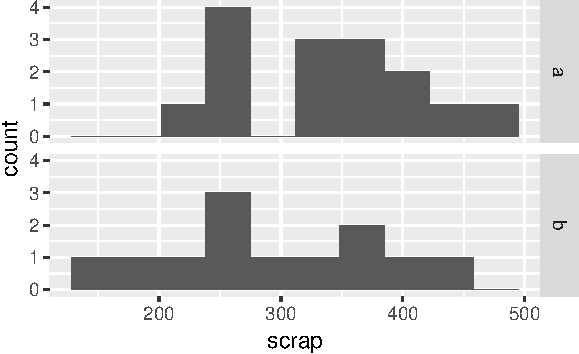
\includegraphics{02-reading-in_files/figure-latex/unnamed-chunk-15-1}

I could have used \texttt{facet\_wrap}, but that would have put the
histograms side by side, and I wanted them one above the other (for ease
of comparison, since they'll be on the same scale). \texttt{facet\_grid}
is like \texttt{facet\_wrap}, but offers you more control over where the
facets go: you can arrange them above and below by a variable, or left
and right by a variable. Whatever is facetting the plots up and down (on
the \(y\) axis) goes before the squiggle, and whatever facets them left
and right goes after. If there is nothing separating the facets in one
direction, here horizontally, the variable is replaced by a dot.

In some ways, \texttt{facet\_grid} is also \emph{less} flexible, because
the facets have to be arranged up/down or left/right by a variable. That
worked here, but if you think back to the Australian athletes, where
there were ten different sports, it was \texttt{facet\_wrap} that did
the right thing, arranging the sports along rows \emph{and} columns to
produce a pleasing display.

All right, that bimodality. I was expecting that the scrap values from
one line would be centred about one value and the scrap values from the
other line would be centred about a different value, with a gap in
between. But that's not what happened at all: the line B values are all
over the place, while it's the line A values that are actually bimodal
all by themselves. I'm not sure whether that really means anything,
since the data sets are pretty small, but it's kind of interesting.

\begin{enumerate}
\def\labelenumi{(\alph{enumi})}
\setcounter{enumi}{5}
\tightlist
\item
  We started out with the suspicion that if the line was run faster,
  there would be more scrap. We haven't assessed this yet. Draw a
  scatter plot with \texttt{scrap} on the \(y\) axis and \texttt{speed}
  on the \(x\) axis.
\end{enumerate}

Solution

Same mechanism as before:

\begin{Shaded}
\begin{Highlighting}[]
\KeywordTok{ggplot}\NormalTok{(soap, }\KeywordTok{aes}\NormalTok{(}\DataTypeTok{x =}\NormalTok{ speed, }\DataTypeTok{y =}\NormalTok{ scrap)) }\OperatorTok{+}\StringTok{ }\KeywordTok{geom_point}\NormalTok{()}
\end{Highlighting}
\end{Shaded}

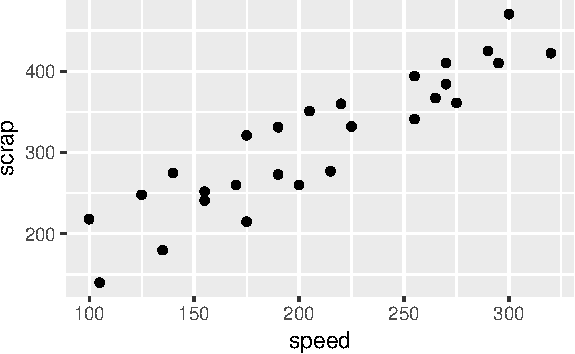
\includegraphics{02-reading-in_files/figure-latex/unnamed-chunk-16-1}

\begin{enumerate}
\def\labelenumi{(\alph{enumi})}
\setcounter{enumi}{6}
\tightlist
\item
  What do you think is the most important conclusion from your plot of
  the previous part? Describe your conclusion in the context of the
  data.
\end{enumerate}

Solution

There seems to be a pretty evident upward trend, apparently linear,
which means that if the speed of the production line is higher, the
amount of scrap produced is also higher. My last sentence was meant to
remind you that ``there is an upward trend'' is \emph{not a complete
answer}: we are concerned with what that upward trend tells us about the
data. This, in other words, confirms the suspicion expressed in the
question, which was therefore a rather large clue: more speed tends to
go with more scrap. That was as far as I wanted you to go: there seems
to be an association with speed, and there might be an association with
\texttt{line} that turned out not to be statistically significant. What
we haven't done is to assess the relationship between speed and scrap
for \emph{each} production line. To do that, we want to plot the
scrap-speed points distinguished for each production line.
\texttt{ggplot} makes that easy: you add a \texttt{colour}
\marginnote{If you are concerned about the spelling: the guy who wrote ggplot is from New Zealand, where they spell *colour* the same way we do. However, if you want to use *color*, that works too.}
to say what you want to distinguish by colour. This is two quantitative
variables and one categorical variable, if you want to think of it that
way:

\begin{Shaded}
\begin{Highlighting}[]
\KeywordTok{ggplot}\NormalTok{(soap, }\KeywordTok{aes}\NormalTok{(}\DataTypeTok{x =}\NormalTok{ speed, }\DataTypeTok{y =}\NormalTok{ scrap, }\DataTypeTok{colour =}\NormalTok{ line)) }\OperatorTok{+}\StringTok{ }
\StringTok{    }\KeywordTok{geom_point}\NormalTok{()}
\end{Highlighting}
\end{Shaded}

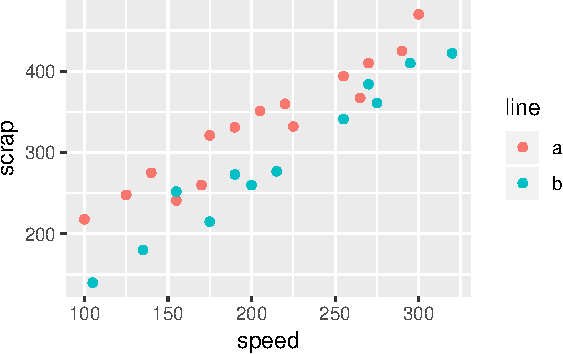
\includegraphics{02-reading-in_files/figure-latex/unnamed-chunk-17-1}

Notice that we get a legend, automatically.

What is interesting about this one is the red dots are mostly at the top
(for any given speed), and the blue dots are mostly at the bottom. That
seems to mean that \emph{when we account for speed}, there is a
difference between lines.

I want to show you one more embellishment, which is to put the
regression lines on the plot for each group separately. This is where
\texttt{ggplot} is so nice, since I just have to add one thing:

\begin{Shaded}
\begin{Highlighting}[]
\KeywordTok{ggplot}\NormalTok{(soap, }\KeywordTok{aes}\NormalTok{(}\DataTypeTok{x =}\NormalTok{ speed, }\DataTypeTok{y =}\NormalTok{ scrap, }\DataTypeTok{colour =}\NormalTok{ line)) }\OperatorTok{+}\StringTok{ }
\StringTok{    }\KeywordTok{geom_point}\NormalTok{() }\OperatorTok{+}\StringTok{ }\KeywordTok{geom_smooth}\NormalTok{(}\DataTypeTok{method =} \StringTok{"lm"}\NormalTok{, }
    \DataTypeTok{se =}\NormalTok{ F)}
\end{Highlighting}
\end{Shaded}

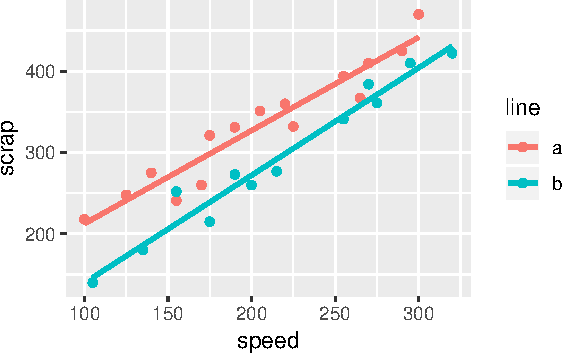
\includegraphics{02-reading-in_files/figure-latex/unnamed-chunk-18-1}

The points and lines have come out in different colours, without our
having to think too hard.

Both lines show an upward trend, with about the same slope, which means
that regardless of line, increasing the speed goes with increasing the
scrap by the same amount. The fact that the red line is above the blue
one, however, suggests that production line A produces more scrap at the
same speed than production line B.

From a management point of view, there is an interesting dynamic at
work: if you run the production line faster, you'll produce more bars of
soap, but you'll produce more scrap as well. The crucial thing for the
people in the supervisor's office is how much raw material is used per
bar of soap, and if you make the soap bars faster, you might use more
raw material, which will eat into your profits (from one angle), but you
will also have more bars of soap to sell.

Here's another way to see the same thing. I'm \emph{definitely} not
expecting you to follow the code, but you can admire the result!

\begin{Shaded}
\begin{Highlighting}[]
\NormalTok{soap2 =}\StringTok{ }\NormalTok{soap }\OperatorTok\StringTok{ }\KeywordTok{select}\NormalTok{(}\OperatorTok{-}\NormalTok{line)}
\KeywordTok{ggplot}\NormalTok{(soap, }\KeywordTok{aes}\NormalTok{(}\DataTypeTok{x =}\NormalTok{ speed, }\DataTypeTok{y =}\NormalTok{ scrap)) }\OperatorTok{+}\StringTok{ }\KeywordTok{geom_point}\NormalTok{(}\DataTypeTok{data =}\NormalTok{ soap2, }
    \DataTypeTok{colour =} \StringTok{"grey"}\NormalTok{) }\OperatorTok{+}\StringTok{ }\KeywordTok{geom_point}\NormalTok{(}\KeywordTok{aes}\NormalTok{(}\DataTypeTok{colour =}\NormalTok{ line)) }\OperatorTok{+}\StringTok{ }
\StringTok{    }\KeywordTok{facet_wrap}\NormalTok{(}\OperatorTok{~}\NormalTok{line)}
\end{Highlighting}
\end{Shaded}

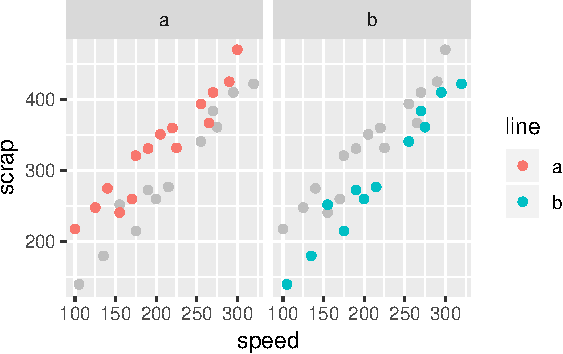
\includegraphics{02-reading-in_files/figure-latex/unnamed-chunk-19-1} \$

The idea is that we plot all the points in grey (to ``put them in the
background'') and then in each plot we plot the points again,
\emph{coloured, for the group we are looking at}: line A in the left,
line B on the right. This is another way of seeing that line A has more
scrap than line B, given the speed at which the line was being run. (I
discovered this technique only yesterday. I think the code is remarkably
concise for what it does.)

The logic of the code is:

\begin{itemize}
\item
  create a new data frame that contains everything in \texttt{soap}
  except for \texttt{line}
\item
  make a scatter plot of all the points in this new data frame, coloured
  grey
\item
  plot the points again (from the original data frame), coloured by
  which production line they're from
\item
  produce a separate scatterplot for each production line.
\end{itemize}

The trick about creating the new data frame was to enable plotting of
all points regardless of group on each subplot (``facet'' in
\texttt{ggplot} terminology), as well as the ones that come from that
production line.

I don't expect you to be able to follow all the details of the code
below, either, but I would like you to try and get the logic. What we do
is a regression predicting \texttt{scrap} from \emph{two} things:
\texttt{speed} and production \texttt{line}. The results we get are
these:

\begin{Shaded}
\begin{Highlighting}[]
\NormalTok{scrap}\FloatTok{.1}\NormalTok{ =}\StringTok{ }\KeywordTok{lm}\NormalTok{(scrap }\OperatorTok{~}\StringTok{ }\NormalTok{speed }\OperatorTok{+}\StringTok{ }\NormalTok{line, }\DataTypeTok{data =}\NormalTok{ soap)}
\KeywordTok{summary}\NormalTok{(scrap}\FloatTok{.1}\NormalTok{)}
\end{Highlighting}
\end{Shaded}

\begin{verbatim}
## 
## Call:
## lm(formula = scrap ~ speed + line, data = soap)
## 
## Residuals:
##     Min      1Q  Median      3Q     Max 
## -39.557 -14.161  -0.121  17.518  33.953 
## 
## Coefficients:
##              Estimate Std. Error t value
## (Intercept)  80.41099   14.54379   5.529
## speed         1.23074    0.06555  18.775
## lineb       -53.12920    8.21003  -6.471
##             Pr(>|t|)    
## (Intercept) 1.10e-05 ***
## speed       7.48e-16 ***
## lineb       1.08e-06 ***
## ---
## Signif. codes:  
##   0 '***' 0.001 '**' 0.01 '*' 0.05 '.' 0.1  ' ' 1
## 
## Residual standard error: 21.13 on 24 degrees of freedom
## Multiple R-squared:  0.9402, Adjusted R-squared:  0.9352 
## F-statistic: 188.6 on 2 and 24 DF,  p-value: 2.104e-15
\end{verbatim}

The P-values for \texttt{speed} and \texttt{line} are the second and
third things in the last column, \(7 \times 10^{-16}\) and
\(1 \times 10^{-6}\) respectively. These are both very strongly
significant, in contrast to the two-sample \(t\)-test where
\texttt{line} was not significant.

So does production line make a difference or not?

The plot says that it does, and the meaning of model \texttt{scrap.1}
just above is that \emph{`speed` affects scrap when you account
for `line`}, and emph\{\texttt{line} affects scrap when you account for
speed\}. (In the two-sample \(t\)-test above we didn't account for speed
at all, since the various speeds were all mixed up.)

There is a moral to this story, which I would like you to get even if
you don't get any of the statistics: if a variable makes a difference,
it should be in your model and on your graph,
\marginnote{Meaning that the graph should contain all three variables, *speed*, *scrap* and *line*.}
because it enables you to get better (more precise) conclusions about
your other variables. Here, there really is a difference between the
production lines, but the \(t\)-test was too much of a blunt instrument
to unearth it (because \texttt{speed} made a difference as well).

\hypertarget{handling-shipments}{%
\section{Handling shipments}\label{handling-shipments}}

A company called Global Electronics from time to time imports shipments
of a certain large part used as a component in several of its products.
The size of the shipment varies each time. Each shipment is sent to one
of two warehouses (labelled A and B) for handling. The data in
\href{http://www.utsc.utoronto.ca/~butler/c32/global.csv}{link} show the
\texttt{size} of each shipment (in thousands of parts) and the direct
\texttt{cost} of handling it, in thousands of dollars. Also shown is the
\texttt{warehouse} (A or B) that handled each shipment.

\begin{enumerate}
\def\labelenumi{(\alph{enumi})}
\tightlist
\item
  Read the data into R and display your data frame. How many rows and
  columns does it have?
\end{enumerate}

Solution

If you open the data file in your web browser, it will probably open as
a spreadsheet, which is not really very helpful, since then it is not
clear what to do with it. You could, I suppose, save it and upload it to
R Studio Cloud, but it requires much less brainpower to open it directly
from the URL:

\begin{Shaded}
\begin{Highlighting}[]
\NormalTok{url =}\StringTok{ "http://www.utsc.utoronto.ca/~butler/c32/global.csv"}
\NormalTok{shipments =}\StringTok{ }\KeywordTok{read_csv}\NormalTok{(url)}
\end{Highlighting}
\end{Shaded}

\begin{verbatim}
## Parsed with column specification:
## cols(
##   warehouse = col_character(),
##   size = col_integer(),
##   cost = col_double()
## )
\end{verbatim}

If you display your data frame and it looks like this, you are good (you
can give the data frame any name):

\begin{Shaded}
\begin{Highlighting}[]
\NormalTok{shipments}
\end{Highlighting}
\end{Shaded}

\begin{verbatim}
## # A tibble: 10 x 3
##    warehouse  size  cost
##    <chr>     <int> <dbl>
##  1 A           225 12.0 
##  2 B           350 14.1 
##  3 A           150  8.93
##  4 A           200 11.0 
##  5 A           175 10.0 
##  6 A           180 10.1 
##  7 B           325 13.8 
##  8 B           290 13.3 
##  9 B           400 15   
## 10 A           125  7.97
\end{verbatim}

It has 10 rows and 3 columns. \emph{You need to say this to get the
mark.}

That is, there were 10 shipments recorded, and for each of them, 3
variables were noted: the size and cost of the shipment, and the
warehouse it was handled at.

\begin{enumerate}
\def\labelenumi{(\alph{enumi})}
\setcounter{enumi}{1}
\tightlist
\item
  Make a scatterplot of the cost of handling each shipment as it depends
  on the shipment's size.
\end{enumerate}

Solution

The wording of the question says that cost is the response and so
belongs on the \(y\)-axis. To make the plot, \texttt{ggplot} with an
\texttt{x=} and a \texttt{y=} in the \texttt{aes} (the ``what to plot''
part), and a \texttt{geom\_point()} after (the ``how to plot it''):

\begin{Shaded}
\begin{Highlighting}[]
\KeywordTok{ggplot}\NormalTok{(shipments, }\KeywordTok{aes}\NormalTok{(}\DataTypeTok{x =}\NormalTok{ size, }\DataTypeTok{y =}\NormalTok{ cost)) }\OperatorTok{+}\StringTok{ }\KeywordTok{geom_point}\NormalTok{()}
\end{Highlighting}
\end{Shaded}

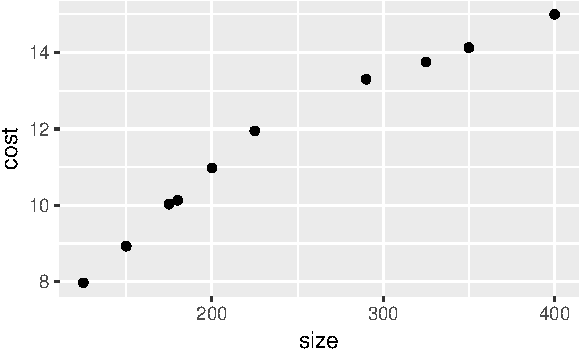
\includegraphics{02-reading-in_files/figure-latex/unnamed-chunk-23-1}

As a matter of coding, there are usually \emph{two} brackets to close
after the \texttt{aes}, the one that begins the \texttt{ggplot} and the
one that begins the \texttt{aes}.

\begin{enumerate}
\def\labelenumi{(\alph{enumi})}
\setcounter{enumi}{2}
\tightlist
\item
  What kind of relationship do you see on the scatterplot? Do you think
  a straight line would describe it appropriately? Explain briefly.
\end{enumerate}

Solution

I see an upward trend: a shipment with larger \texttt{size} costs more
to handle. If you look carefully at the scatterplot, you see that the
cost of handling a small shipment goes up fairly steeply with its size,
but the cost of handling a large shipment, while it still increases with
\texttt{size}, does not increase so fast. Thus having one straight line
to describe the whole relationship would not work so well. The
relationship is actually two different straight lines joined end-to-end,
which we will explore later, but if you think the relationship is
curved, I'll accept that. The point is to get at the idea that the rate
of increase is not constant.

\begin{enumerate}
\def\labelenumi{(\alph{enumi})}
\setcounter{enumi}{3}
\tightlist
\item
  When a shipment comes in, the cost of handling it is not known. A
  decision is made about which warehouse to send it to, and then, after
  it is handled, the cost is recorded. What do you think determines
  which warehouse an incoming shipment goes to? Provide a graph to
  support your answer.
\end{enumerate}

Solution

The veiled hint in the question is that the decision must depend on
\texttt{size}, since it cannot depend on \texttt{cost}. So we have one
quantitative variable \texttt{size} and one categorical variable
\texttt{warehouse}, which suggests drawing boxplots:

\begin{Shaded}
\begin{Highlighting}[]
\KeywordTok{ggplot}\NormalTok{(shipments, }\KeywordTok{aes}\NormalTok{(}\DataTypeTok{x =}\NormalTok{ warehouse, }\DataTypeTok{y =}\NormalTok{ size)) }\OperatorTok{+}\StringTok{ }
\StringTok{    }\KeywordTok{geom_boxplot}\NormalTok{()}
\end{Highlighting}
\end{Shaded}

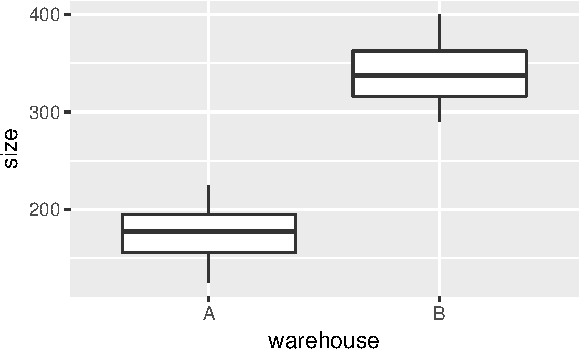
\includegraphics{02-reading-in_files/figure-latex/unnamed-chunk-24-1}

Well, there's the answer right there. When the shipment has small
\texttt{size}, it goes to warehouse A, and when it's large, it goes to
Warehouse B. We know this because \emph{all} the shipments smaller than
about 250 (thousand parts) went to A and \emph{all} the shipments larger
than that went to B. (If you want to provide a number to delineate
``small'' and ``large'', anything between the largest A, about 225, and
the smallest B, about 290, will do.)

Another way to think about this is to add something to the scatterplot
you drew before. The obvious thing is to make the two warehouses
different colours:

\begin{Shaded}
\begin{Highlighting}[]
\KeywordTok{ggplot}\NormalTok{(shipments, }\KeywordTok{aes}\NormalTok{(}\DataTypeTok{x =}\NormalTok{ size, }\DataTypeTok{y =}\NormalTok{ cost, }\DataTypeTok{colour =}\NormalTok{ warehouse)) }\OperatorTok{+}\StringTok{ }
\StringTok{    }\KeywordTok{geom_point}\NormalTok{()}
\end{Highlighting}
\end{Shaded}

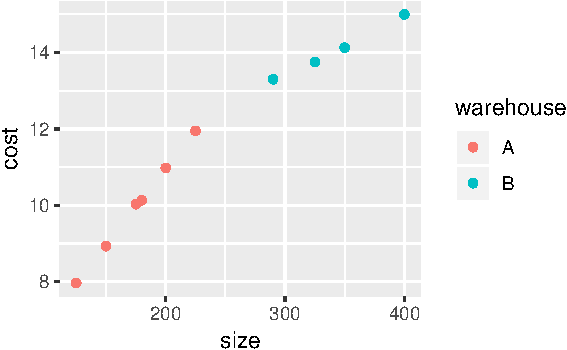
\includegraphics{02-reading-in_files/figure-latex/unnamed-chunk-25-1}

As a point of technique, you can split lines of code to make them fit on
your screen. You can do this as long as \emph{the code that ends
the line must be incomplete}, so that R knows more is to come. Ending a
line with a pipe symbol, or, as here, with one of the pluses in the
middle of a \texttt{ggplot}, will work. If you put the plus on the start
of the next line, you'll get a blank plot, because R thinks you're done
plotting. Try it and see.

Anyway, this plot tells exactly the same story: the small shipments (in
size or cost) go to Warehouse A and the large ones to Warehouse B. But
we don't know cost when the decision is made about which warehouse to
send a shipment to, so the decision must be based on \texttt{size}.

In the place where I got these data, it said ``larger shipments are sent
to Warehouse B, since this warehouse has specialized equipment that
provides greater economies of scale for larger shipments''. That is to
say, very large shipments are more expensive to handle, but not as
expensive as you might think.
\marginnote{This is the same idea that it  costs more to ride the GO bus from UTSC to York U than it does to  ride from UTSC to Scarborough Town, but if you work out how much it  costs per kilometre, the longer journey costs less per km. As of  when I'm writing this, $5.30 for the 7.2 km to Scarborough Town and  $6.75 for the 38 km to York. That's quite an economy of scale,  isn't it?}
That makes sense with our scatterplot, because the \emph{slope} for
larger shipments is less than for smaller shipments.

When we get to regression later, we'll see what happens if we fit a
straight line to data like these, and how to tell whether we really
ought to be able to do better with a different form of relationship.
There is also a trick to fit what is called a ``piecewise linear
regression'', which has one slope for small shipment sizes, a different
(smaller) slope for large ones, and joins up in the middle. But that's
well beyond our scope now.

\hypertarget{data-exploration}{%
\chapter{Data exploration}\label{data-exploration}}

\begin{Shaded}
\begin{Highlighting}[]
\KeywordTok{library}\NormalTok{(tidyverse)}
\end{Highlighting}
\end{Shaded}

\begin{verbatim}
## -- Attaching packages ---- tidyverse 1.2.1 --
\end{verbatim}

\begin{verbatim}
## v ggplot2 3.1.0     v purrr   0.2.5
## v tibble  1.4.2     v dplyr   0.7.8
## v tidyr   0.8.1     v stringr 1.3.1
## v readr   1.1.1     v forcats 0.3.0
\end{verbatim}

\begin{verbatim}
## -- Conflicts ------- tidyverse_conflicts() --
## x dplyr::filter() masks stats::filter()
## x dplyr::lag()    masks stats::lag()
\end{verbatim}

\hypertarget{north-carolina-births}{%
\section{North Carolina births}\label{north-carolina-births}}

The data in file
\href{http://www.utsc.utoronto.ca/~butler/c32/ncbirths.csv}{link} are
about 500 randomly chosen births of babies in North Carolina. There is a
lot of information: not just the weight at birth of the baby, but
whether the baby was born prematurely, the ages of the parents, whether
the parents are married, how long (in weeks) the pregnancy lasted (this
is called the ``gestation'') and so on.

\begin{enumerate}
\def\labelenumi{(\alph{enumi})}
\tightlist
\item
  Read in the data from the file into R, bearing in mind what type of
  file it is.
\end{enumerate}

Solution

This is a \texttt{.csv} file (it came from a spreadsheet), so it needs
reading in accordingly. Work directly from the URL (rather than
downloading the file, unless you are working offline):

\begin{Shaded}
\begin{Highlighting}[]
\NormalTok{myurl =}\StringTok{ "http://www.utsc.utoronto.ca/~butler/c32/ncbirths.csv"}
\NormalTok{bw =}\StringTok{ }\KeywordTok{read_csv}\NormalTok{(myurl)}
\end{Highlighting}
\end{Shaded}

\begin{verbatim}
## Parsed with column specification:
## cols(
##   `Father Age` = col_integer(),
##   `Mother Age` = col_integer(),
##   `Weeks Gestation` = col_integer(),
##   `Pre-natal Visits` = col_integer(),
##   `Marital Status` = col_integer(),
##   `Mother Weight Gained` = col_integer(),
##   `Low Birthweight?` = col_integer(),
##   `Weight (pounds)` = col_double(),
##   `Premie?` = col_integer(),
##   `Few Visits?` = col_integer()
## )
\end{verbatim}

This shows you which variables the data set has (some of the names got a
bit mangled), and it shows you that they are all integers except for the
birth weight (a decimal number).

The easiest way to find out how many rows and columns there are is
simply to list the data frame:

\begin{Shaded}
\begin{Highlighting}[]
\NormalTok{bw}
\end{Highlighting}
\end{Shaded}

\begin{verbatim}
## # A tibble: 500 x 10
##    `Father Age` `Mother Age` `Weeks Gestatio~
##           <int>        <int>            <int>
##  1           27           26               38
##  2           35           33               40
##  3           34           22               37
##  4           NA           16               38
##  5           35           33               39
##  6           32           24               36
##  7           33           33               38
##  8           38           35               38
##  9           28           29               40
## 10           NA           19               34
## # ... with 490 more rows, and 7 more
## #   variables: `Pre-natal Visits` <int>,
## #   `Marital Status` <int>, `Mother Weight
## #   Gained` <int>, `Low Birthweight?` <int>,
## #   `Weight (pounds)` <dbl>,
## #   `Premie?` <int>, `Few Visits?` <int>
\end{verbatim}

or you can take a ``glimpse'' of it:

\begin{Shaded}
\begin{Highlighting}[]
\KeywordTok{glimpse}\NormalTok{(bw)}
\end{Highlighting}
\end{Shaded}

\begin{verbatim}
## Observations: 500
## Variables: 10
## $ `Father Age`           <int> 27, 35, 3...
## $ `Mother Age`           <int> 26, 33, 2...
## $ `Weeks Gestation`      <int> 38, 40, 3...
## $ `Pre-natal Visits`     <int> 14, 11, 1...
## $ `Marital Status`       <int> 1, 1, 2, ...
## $ `Mother Weight Gained` <int> 32, 23, 5...
## $ `Low Birthweight?`     <int> 0, 0, 0, ...
## $ `Weight (pounds)`      <dbl> 6.8750, 6...
## $ `Premie?`              <int> 0, 0, 0, ...
## $ `Few Visits?`          <int> 0, 0, 0, ...
\end{verbatim}

Either of these displays show that there are 500 rows (observations,
here births) and 10 columns (variables), and they both show what the
variables are called. So they're both good as an answer to the question.

What you'll notice is that the variables have \emph{spaces} in their
names, which will require special handling later. These outputs show you
what to do about those spaces in variable names: surround the variable
name with ``backticks''. (On my keyboard, that's on the key to the left
of number 1, where the squiggle is, that looks like a backwards
apostrophe. Probably next to \texttt{Esc}, depending on the layout of
your keyboard.)

Although almost all of the variables are stored as integers, the ones
that have a question mark in their name are actually ``logical'', true
or false, with 1 denoting true and 0 false. We could convert them later
if we want to. (A question mark is not a traditional character to put in
a variable name, so we have to surround these variables with backticks
too.)

\begin{enumerate}
\def\labelenumi{(\alph{enumi})}
\setcounter{enumi}{1}
\tightlist
\item
  From your output, verify that you have the right number of
  observations and that you have several variables. Which of your
  variables correspond to birthweight, prematureness and length of
  pregnancy? (You might have to make guesses based on the names of the
  variables.)
\end{enumerate}

Solution

I do indeed have 500 observations on 10 variables (``several''). (If you
don't have several variables, check to see that you didn't use
\texttt{read\_delim} or something by mistake.) After the ``500
observations of 10 variables'' line(s) in each case, you see all the
variables by name, with what type of values they have,
\marginnote{these    are mostly *int* or *integer*.} and the first few
of the values.
\marginnote{Other possible variable types are *num* for    (real, decimal) numbers such as birth weight, *chr* for    text, and *Factor* (with the number of levels) for    factors/categorical variables. We don't have any of the last two    here. There is also *lgl* for *logical*, things that were    actually recorded as TRUE or FALSE. We have some variables that    are actually logical ones, but they are recorded as integer    values.}

The variable \texttt{Weight\ (pounds)} is the birthweight (in pounds),
\texttt{Premie?} is 1 for a premature baby and 0 for a full-term baby,
and \texttt{Weeks\ Gestation} is the number of weeks the pregnancy
lasted. Don't forget to put backticks around each of those when you use
them later.
\marginnote{The backticks look different from each other for  annoying technical reasons, but they're all backticks.}

\begin{enumerate}
\def\labelenumi{(\alph{enumi})}
\setcounter{enumi}{2}
\tightlist
\item
  The theory behind the \(t\)-test (which we do later) says that the
  distribution of birth weights should be (approximately) normally
  distributed. Obtain a histogram of the birth weights. Does it look
  approximately normal? Comment briefly. (You'll have to pick a number
  of bins for your histogram first. I don't mind very much what you
  pick, as long as it's not obviously too many or too few bins.)
\end{enumerate}

Solution

You'll have seen that I often start with 10 bins, or maybe not quite
that many if I don't have much data, and this is a decent general
principle. That would give

\begin{Shaded}
\begin{Highlighting}[]
\KeywordTok{ggplot}\NormalTok{(bw, }\KeywordTok{aes}\NormalTok{(}\DataTypeTok{x =} \StringTok{`}\DataTypeTok{Weight (pounds)}\StringTok{`}\NormalTok{)) }\OperatorTok{+}\StringTok{ }\KeywordTok{geom_histogram}\NormalTok{(}\DataTypeTok{bins =} \DecValTok{10}\NormalTok{)}
\end{Highlighting}
\end{Shaded}

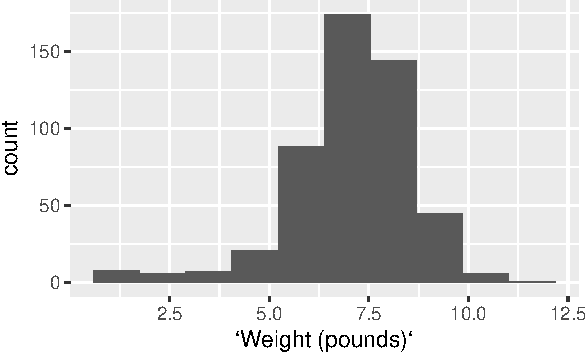
\includegraphics{03-data-summaries_files/figure-latex/unnamed-chunk-10-1}

which is perfectly acceptable. You can try something a bit more or a bit
less, and see how you like it in comparison. What you are looking for is
a nice clear picture of \emph{shape}. If you have too few bins, you'll
lose the shape:

\begin{Shaded}
\begin{Highlighting}[]
\KeywordTok{ggplot}\NormalTok{(bw, }\KeywordTok{aes}\NormalTok{(}\DataTypeTok{x =} \StringTok{`}\DataTypeTok{Weight (pounds)}\StringTok{`}\NormalTok{)) }\OperatorTok{+}\StringTok{ }\KeywordTok{geom_histogram}\NormalTok{(}\DataTypeTok{bins =} \DecValTok{4}\NormalTok{)}
\end{Highlighting}
\end{Shaded}

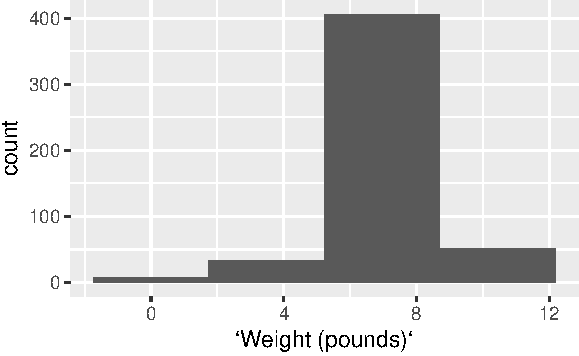
\includegraphics{03-data-summaries_files/figure-latex/unnamed-chunk-11-1}

(is that leftmost bin an indication of skewness or some observations
that happen to be smallish?)

And if you have too many, the shape will be there, but it will be hard
to make out in all the noise, with frequencies going up and down:

\begin{Shaded}
\begin{Highlighting}[]
\KeywordTok{ggplot}\NormalTok{(bw, }\KeywordTok{aes}\NormalTok{(}\DataTypeTok{x =} \StringTok{`}\DataTypeTok{Weight (pounds)}\StringTok{`}\NormalTok{)) }\OperatorTok{+}\StringTok{ }\KeywordTok{geom_histogram}\NormalTok{(}\DataTypeTok{bins =} \DecValTok{30}\NormalTok{)}
\end{Highlighting}
\end{Shaded}

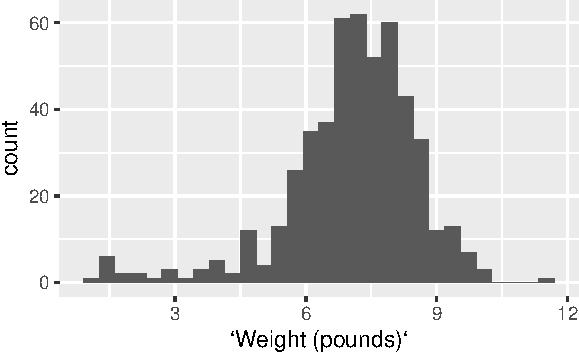
\includegraphics{03-data-summaries_files/figure-latex/unnamed-chunk-12-1}

I generally am fairly relaxed about the number of bins you use, as long
as it's not clearly too few or too many. You might have done exercises
in the past that illustrate that the choice of number of bins (or the
class intervals where you move from one bin to the next, which is
another issue that I won't explore here) can make an appreciable
difference to how a histogram looks. Extra: I had some thoughts about
this issue that I put in a blog post, that you might like to read:
\href{http://ritsokiguess.site/docs/2017/06/08/histograms-and-bins/}{link}.
The nice thing about Sturges' rule, mentioned there, is that you can
almost get a number of bins for your histogram in your head (as long as
you know the powers of 2, that is). What you do is to start with your
sample size, here \(n=500\). You find the next power of 2 above that,
which is here \(512=2^9\). You then take that power and add 1, to get 10
bins. If you don't like that, you can get R to calculate it for you:

\begin{Shaded}
\begin{Highlighting}[]
\KeywordTok{nclass.Sturges}\NormalTok{(bw}\OperatorTok{$}\StringTok{`}\DataTypeTok{Weight (pounds)}\StringTok{`}\NormalTok{)}
\end{Highlighting}
\end{Shaded}

\begin{verbatim}
## [1] 10
\end{verbatim}

The place where Sturges' rule comes from is an assumption of normal data
(actually a binomial approximation to the normal, backwards though that
sounds). If you have less than 30 observations, you'll get fewer than 6
bins, which won't do much of a job of showing the shape. Rob Hyndman
wrote a \href{https://robjhyndman.com/papers/sturges.pdf}{critical note}
about Sturges' rule in which he asserts that it is just plain wrong (if
you have taken B57, this note is very readable).

So what to use instead? Well, judgment is still better than something
automatic, but if you want a place to start from, something with a
better foundation than Sturges is the Freedman-Diaconis rule. This, in
its original formulation, gives a bin width rather than a number of
bins:

\[ 
w=2(IQR)n^{-1/3}
\]

The nice thing about this is that it uses the interquartile range, so it
won't be distorted by outliers. \texttt{geom\_histogram} can take a bin
width, so we can use it as follows:

\begin{Shaded}
\begin{Highlighting}[]
\NormalTok{w =}\StringTok{ }\DecValTok{2} \OperatorTok{*}\StringTok{ }\KeywordTok{IQR}\NormalTok{(bw}\OperatorTok{$}\StringTok{`}\DataTypeTok{Weight (pounds)}\StringTok{`}\NormalTok{) }\OperatorTok{*}\StringTok{ }\DecValTok{500}\OperatorTok{^}\NormalTok{(}\OperatorTok{-}\DecValTok{1}\OperatorTok{/}\DecValTok{3}\NormalTok{)}
\NormalTok{w}
\end{Highlighting}
\end{Shaded}

\begin{verbatim}
## [1] 0.4094743
\end{verbatim}

\begin{Shaded}
\begin{Highlighting}[]
\KeywordTok{ggplot}\NormalTok{(bw, }\KeywordTok{aes}\NormalTok{(}\DataTypeTok{x =} \StringTok{`}\DataTypeTok{Weight (pounds)}\StringTok{`}\NormalTok{)) }\OperatorTok{+}\StringTok{ }\KeywordTok{geom_histogram}\NormalTok{(}\DataTypeTok{binwidth =}\NormalTok{ w)}
\end{Highlighting}
\end{Shaded}

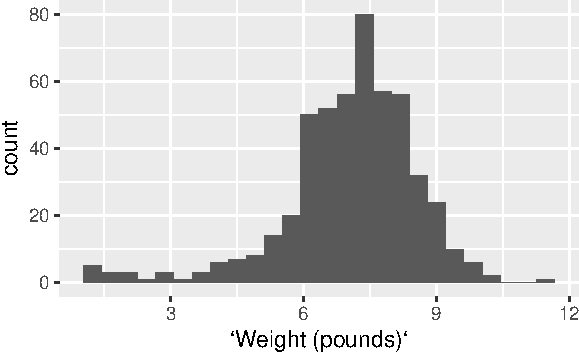
\includegraphics{03-data-summaries_files/figure-latex/unnamed-chunk-14-1}

R also has

\begin{Shaded}
\begin{Highlighting}[]
\NormalTok{nc =}\StringTok{ }\KeywordTok{nclass.FD}\NormalTok{(bw}\OperatorTok{$}\StringTok{`}\DataTypeTok{Weight (pounds)}\StringTok{`}\NormalTok{)}
\NormalTok{nc}
\end{Highlighting}
\end{Shaded}

\begin{verbatim}
## [1] 26
\end{verbatim}

which turns the Freedman-Diaconis rule into a number of bins rather than
a binwidth; using that gives the same histogram as we got with
\texttt{binwidth}.

In my opinion, Freedman-Diaconis tends to give too many bins (here there
are 26 rather than the 10 of Sturges). But I put it out there for you to
make your own call.

Another way to go is a ``density plot''. This is a smoothed-out version
of a histogram that is not obviously frequencies in bins, but which does
have a theoretical basis. It goes something like this:

\begin{Shaded}
\begin{Highlighting}[]
\KeywordTok{ggplot}\NormalTok{(bw, }\KeywordTok{aes}\NormalTok{(}\DataTypeTok{x =} \StringTok{`}\DataTypeTok{Weight (pounds)}\StringTok{`}\NormalTok{)) }\OperatorTok{+}\StringTok{ }\KeywordTok{geom_density}\NormalTok{()}
\end{Highlighting}
\end{Shaded}

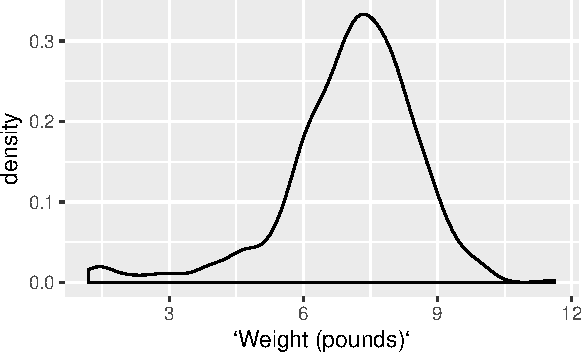
\includegraphics{03-data-summaries_files/figure-latex/unnamed-chunk-16-1}

\texttt{geom\_density} has an optional parameter that controls how
smooth or wiggly the picture is, but the default is usually good.

Alright, before we got distracted, we were assessing normality. What
about that?

It is mostly normal-looking, but I am suspicious about those \emph{very}
low birth weights, the ones below about 4 pounds. There are a few too
many of those, as I see it.

If you think this is approximately normal, you need to make some comment
along the lines of ``the shape is approximately symmetric with no
outliers''. I think my first answer is better, but this answer is worth
something, since it is a not completely unreasonable interpretation of
the histogram.

I have been making the distinction between a histogram (for one
quantitative variable) and side-by-side boxplots (for one quantitative
variable divided into groups by one categorical variable). When you
learned the boxplot, you probably learned it in the context of one
quantitative variable. You can draw a boxplot for that, too, but the
\texttt{ggplot} boxplot has an \texttt{x} as well as a \texttt{y}. What
you do to make a single boxplot is to set the \texttt{x} equal 1, which
produces a weird \(x\)-axis (that you ignore):

\begin{Shaded}
\begin{Highlighting}[]
\KeywordTok{ggplot}\NormalTok{(bw, }\KeywordTok{aes}\NormalTok{(}\DataTypeTok{x =} \DecValTok{1}\NormalTok{, }\DataTypeTok{y =} \StringTok{`}\DataTypeTok{Weight (pounds)}\StringTok{`}\NormalTok{)) }\OperatorTok{+}\StringTok{ }
\StringTok{    }\KeywordTok{geom_boxplot}\NormalTok{()}
\end{Highlighting}
\end{Shaded}

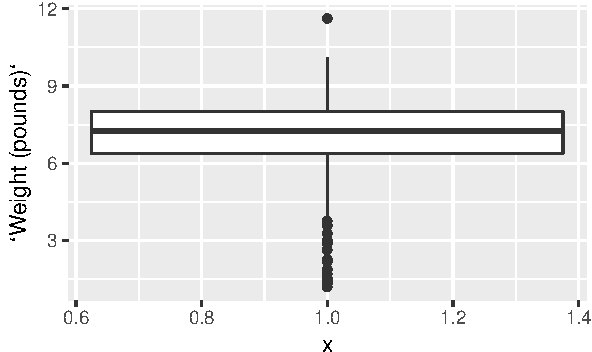
\includegraphics{03-data-summaries_files/figure-latex/unnamed-chunk-17-1}

The high weight is actually an outlier, but look at all those outliers
at the bottom!
\marginnote{When Tukey, a name we will see again, invented  the boxplot in the 1950s, 500 observations would have been  considered a big data set. He designed the boxplot to produce a  sensible number of outliers for the typical size of data set of his  day, but a boxplot of a large data set tends to have a lot of  outliers that are probably not really outliers at all.}

\emph{I} think the reason for those extra very low values is that they
are the premature births (that can result in \emph{very} small babies).
Which leads to the additional question coming up.

\hypertarget{more-about-the-nc-births}{%
\section{More about the NC births}\label{more-about-the-nc-births}}

This is an exploration of some extra issues around the North Carolina
births data set.

\begin{enumerate}
\def\labelenumi{(\alph{enumi})}
\tightlist
\item
  How short does a pregnancy have to be, for the birth to be classified
  as ``premature''? Deduce this from the data, by drawing a suitable
  graph or otherwise.
\end{enumerate}

Solution

To figure it out from the data, we can see how \texttt{Weeks\ Gestation}
depends on \texttt{Premie?}. Some possibilities are boxplots or a
scatterplot. Either of the first two graphs would get full credit (for
the graphing part: you still have to do the explanation) if this were
being marked:

\begin{Shaded}
\begin{Highlighting}[]
\KeywordTok{ggplot}\NormalTok{(bw, }\KeywordTok{aes}\NormalTok{(}\DataTypeTok{x =} \KeywordTok{factor}\NormalTok{(}\StringTok{`}\DataTypeTok{Premie?}\StringTok{`}\NormalTok{), }\DataTypeTok{y =} \StringTok{`}\DataTypeTok{Weeks Gestation}\StringTok{`}\NormalTok{)) }\OperatorTok{+}\StringTok{ }
\StringTok{    }\KeywordTok{geom_boxplot}\NormalTok{()}
\end{Highlighting}
\end{Shaded}

\begin{verbatim}
## Warning: Removed 1 rows containing non-finite
## values (stat_boxplot).
\end{verbatim}

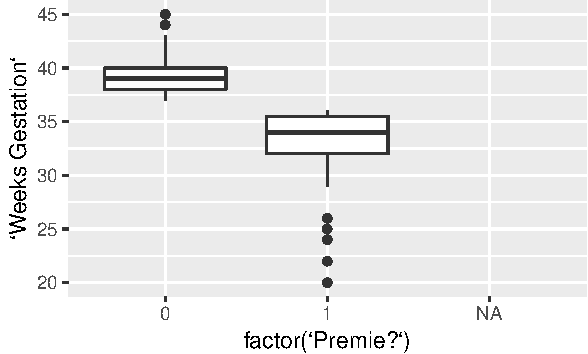
\includegraphics{03-data-summaries_files/figure-latex/unnamed-chunk-18-1}

The warning is because the prematurity of one of the babies is not
known. Or

\begin{Shaded}
\begin{Highlighting}[]
\KeywordTok{ggplot}\NormalTok{(bw, }\KeywordTok{aes}\NormalTok{(}\DataTypeTok{x =} \StringTok{`}\DataTypeTok{Premie?}\StringTok{`}\NormalTok{, }\DataTypeTok{y =} \StringTok{`}\DataTypeTok{Weeks Gestation}\StringTok{`}\NormalTok{)) }\OperatorTok{+}\StringTok{ }
\StringTok{    }\KeywordTok{geom_point}\NormalTok{()}
\end{Highlighting}
\end{Shaded}

\begin{verbatim}
## Warning: Removed 1 rows containing missing values
## (geom_point).
\end{verbatim}

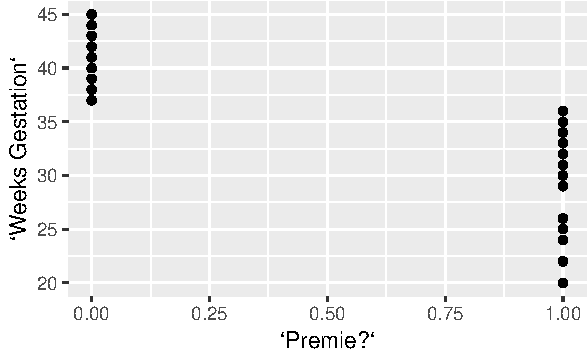
\includegraphics{03-data-summaries_files/figure-latex/unnamed-chunk-19-1}

The same warning again, for the same reason.

Notice how the graphs are similar in syntax, because the what-to-plot is
the same (apart from the \texttt{factor} thing) and we just make a small
change in how-to-plot-it. In the boxplot, the thing on the \(x\)-scale
needs to be categorical, and \texttt{Premie?} is actually a number, so
we'd better make it into a \texttt{factor}, which is R's version of a
categorical variable. \texttt{Premie.} is actually a categorical
variable (``premature'' or ``not premature'') masquerading as a
quantitative one (1 or 0). It is an ``indicator variable'', if you're
familiar with that term.

It looks as if the breakpoint is 37 weeks: a pregnancy at least that
long is considered normal, but a shorter one ends with a premature
birth. Both plots show the same thing: the `\texttt{Premie?}=1` births
all go with short pregnancies, shorter than 37 weeks. This is completely
clear cut.

Another way to attack this is to use \texttt{summarize}, finding the max
and min:

\begin{Shaded}
\begin{Highlighting}[]
\NormalTok{bw }\OperatorTok\StringTok{ }\KeywordTok{summarize}\NormalTok{(}\DataTypeTok{n =} \KeywordTok{n}\NormalTok{(), }\DataTypeTok{min =} \KeywordTok{min}\NormalTok{(}\StringTok{`}\DataTypeTok{Weeks Gestation}\StringTok{`}\NormalTok{), }
    \DataTypeTok{max =} \KeywordTok{max}\NormalTok{(}\StringTok{`}\DataTypeTok{Weeks Gestation}\StringTok{`}\NormalTok{))}
\end{Highlighting}
\end{Shaded}

\begin{verbatim}
## # A tibble: 1 x 3
##       n   min   max
##   <int> <dbl> <dbl>
## 1   500    NA    NA
\end{verbatim}

only this is for \emph{all} the babies, premature or not.
\marginnote{I  explain the missing values below.} So we want it by
prematurity, which means a \texttt{group\_by} first:

\begin{Shaded}
\begin{Highlighting}[]
\NormalTok{bw }\OperatorTok\StringTok{ }\KeywordTok{group_by}\NormalTok{(}\StringTok{`}\DataTypeTok{Premie?}\StringTok{`}\NormalTok{) }\OperatorTok\StringTok{ }\KeywordTok{summarize}\NormalTok{(}\DataTypeTok{n =} \KeywordTok{n}\NormalTok{(), }
    \DataTypeTok{min =} \KeywordTok{min}\NormalTok{(}\StringTok{`}\DataTypeTok{Weeks Gestation}\StringTok{`}\NormalTok{), }\DataTypeTok{max =} \KeywordTok{max}\NormalTok{(}\StringTok{`}\DataTypeTok{Weeks Gestation}\StringTok{`}\NormalTok{))}
\end{Highlighting}
\end{Shaded}

\begin{verbatim}
## # A tibble: 3 x 4
##   `Premie?`     n   min   max
##       <int> <int> <dbl> <dbl>
## 1         0   424    37    45
## 2         1    75    20    36
## 3        NA     1    NA    NA
\end{verbatim}

\texttt{group\_by} with a number works, even though using the number in
\texttt{Premie?} in a boxplot didn't. \texttt{group\_by} just uses the
distinct values, whether they are numbers, text or factor levels.

Any of these graphs or summaries will help you answer the question, in
the same way. The ultimate issue here is ``something that will get the
job done'': it doesn't matter so much what.

In R, \texttt{NA} means ``missing''. When you try to compute something
containing a missing value, the answer is usually missing (since you
don't know what the missing value is). That's why the first
\texttt{summarize} gave us missing values: there was one missing weeks
of gestation in with all the ones for which we had values, so the max
and min had to be missing as well. In the second \texttt{summarize}, the
one by whether a baby was born prematurely or not, we learn a bit more
about that missing \texttt{Premie?}: evidently its weeks of gestation
was missing as well, since the min and max of that were missing.
\marginnote{If there had been a weeks of gestation, we could have figured out whether it was premature or not, according to whether the weeks of gestation was less than 37.}

Here's that baby. I'm doing a bit of fiddling to show all the columns
(as rows, since there's only one actual row). Don't worry about the
second line of code below; we will investigate that later.

\begin{Shaded}
\begin{Highlighting}[]
\NormalTok{bw }\OperatorTok\StringTok{ }\KeywordTok{filter}\NormalTok{(}\KeywordTok{is.na}\NormalTok{(}\StringTok{`}\DataTypeTok{Premie?}\StringTok{`}\NormalTok{)) }\OperatorTok\StringTok{ }\KeywordTok{gather}\NormalTok{(name, }
\NormalTok{    value, }\KeywordTok{everything}\NormalTok{())}
\end{Highlighting}
\end{Shaded}

\begin{verbatim}
## # A tibble: 10 x 2
##    name                 value
##    <chr>                <dbl>
##  1 Father Age           33   
##  2 Mother Age           32   
##  3 Weeks Gestation      NA   
##  4 Pre-natal Visits      9   
##  5 Marital Status        1   
##  6 Mother Weight Gained 25   
##  7 Low Birthweight?      0   
##  8 Weight (pounds)       7.19
##  9 Premie?              NA   
## 10 Few Visits?           0
\end{verbatim}

The \emph{only} thing that was missing was its weeks of gestation, but
that prevented anyone from figuring out whether it was premature or not.

\begin{enumerate}
\def\labelenumi{(\alph{enumi})}
\setcounter{enumi}{1}
\tightlist
\item
  Explore the relationship between birth weight and length of pregancy
  (``gestation'') using a suitable graph. What do you see?
\end{enumerate}

Solution

This needs to be a scatterplot because these are both quantitative
variables:

\begin{Shaded}
\begin{Highlighting}[]
\KeywordTok{ggplot}\NormalTok{(bw, }\KeywordTok{aes}\NormalTok{(}\DataTypeTok{x =} \StringTok{`}\DataTypeTok{Weeks Gestation}\StringTok{`}\NormalTok{, }\DataTypeTok{y =} \StringTok{`}\DataTypeTok{Weight (pounds)}\StringTok{`}\NormalTok{)) }\OperatorTok{+}\StringTok{ }
\StringTok{    }\KeywordTok{geom_point}\NormalTok{()}
\end{Highlighting}
\end{Shaded}

\begin{verbatim}
## Warning: Removed 1 rows containing missing values
## (geom_point).
\end{verbatim}

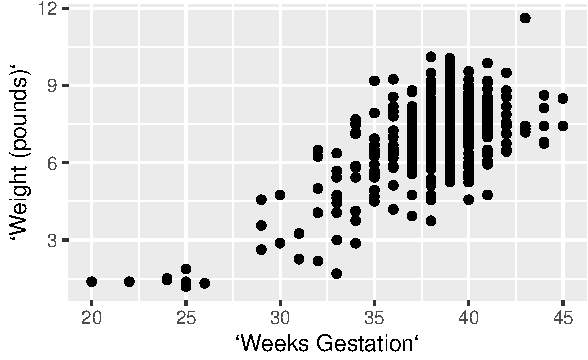
\includegraphics{03-data-summaries_files/figure-latex/unnamed-chunk-23-1}

You see a rather clear upward trend. Those very underweight babies came
from very short pregnancies, but the vast majority of pregnancies were
of more or less normal length (40 weeks is normal) and resulted in
babies of more or less normal birth weight.

I want to illustrate something else: how about \emph{colouring} the
births that were premature? Piece of cake with \texttt{ggplot}:

\begin{Shaded}
\begin{Highlighting}[]
\KeywordTok{ggplot}\NormalTok{(bw, }\KeywordTok{aes}\NormalTok{(}\DataTypeTok{x =} \StringTok{`}\DataTypeTok{Weeks Gestation}\StringTok{`}\NormalTok{, }\DataTypeTok{y =} \StringTok{`}\DataTypeTok{Weight (pounds)}\StringTok{`}\NormalTok{, }
    \DataTypeTok{colour =} \StringTok{`}\DataTypeTok{Premie?}\StringTok{`}\NormalTok{)) }\OperatorTok{+}\StringTok{ }\KeywordTok{geom_point}\NormalTok{()}
\end{Highlighting}
\end{Shaded}

\begin{verbatim}
## Warning: Removed 1 rows containing missing values
## (geom_point).
\end{verbatim}

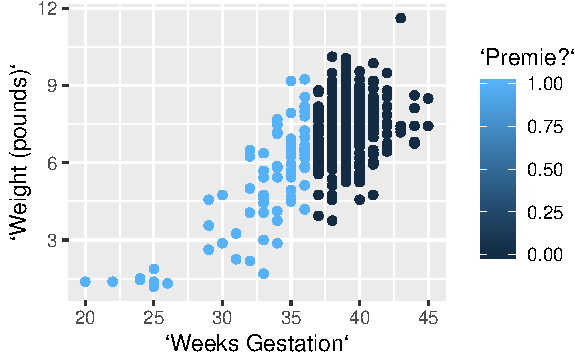
\includegraphics{03-data-summaries_files/figure-latex/unnamed-chunk-24-1}

That was rather silly because \texttt{ggplot} treated prematureness as a
\emph{continuous} variable, and plotted the values on a dark blue-light
blue scale. This is the same issue as on the boxplot above, and has the
same solution:

\begin{Shaded}
\begin{Highlighting}[]
\KeywordTok{ggplot}\NormalTok{(bw, }\KeywordTok{aes}\NormalTok{(}\DataTypeTok{x =} \StringTok{`}\DataTypeTok{Weeks Gestation}\StringTok{`}\NormalTok{, }\DataTypeTok{y =} \StringTok{`}\DataTypeTok{Weight (pounds)}\StringTok{`}\NormalTok{, }
    \DataTypeTok{colour =} \KeywordTok{factor}\NormalTok{(}\StringTok{`}\DataTypeTok{Premie?}\StringTok{`}\NormalTok{))) }\OperatorTok{+}\StringTok{ }\KeywordTok{geom_point}\NormalTok{()}
\end{Highlighting}
\end{Shaded}

\begin{verbatim}
## Warning: Removed 1 rows containing missing values
## (geom_point).
\end{verbatim}

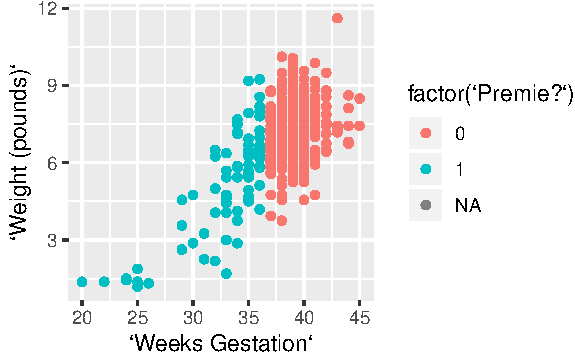
\includegraphics{03-data-summaries_files/figure-latex/unnamed-chunk-25-1}

Better.

With the normal-length pregnancies (red), there seems to be no
relationship between length of pregnancy and birth weight, just a random
variation. But with the premature births, a shorter pregnancy typically
goes with a \emph{lower} birth weight. This would be why the birth
weights for the premature births were more variable.

\begin{enumerate}
\def\labelenumi{(\alph{enumi})}
\setcounter{enumi}{2}
\tightlist
\item
  Do a web search to find the standard (North American) definition of a
  premature birth. Does that correspond to what you saw in the data?
  Cite the website you used, for example by saying ``according to
  \texttt{URL}, ldots'', with \texttt{URL} replaced by the address of
  the website you found.
\end{enumerate}

Solution

The website
\url{http://www.mayoclinic.org/diseases-conditions/premature-birth/basics/definition/con-20020050}
says that ``a premature birth is one that occurs before the start of the
37th week of pregnancy'', which is exactly what we found. (Note that I
am citing the webpage on which I found this, and I even made it into a
link so that you can check it.) The Mayo Clinic is a famous hospital
system with locations in several US states, so I think we can trust what
its website says.

\hypertarget{nenana-alaska}{%
\section{Nenana, Alaska}\label{nenana-alaska}}

Nenana, Alaska, is about 50 miles west of Fairbanks. Every spring, there
is a contest in Nenana. A wooden tripod is placed on the frozen river,
and people try to guess the exact minute when the ice melts enough for
the tripod to fall through the ice. The contest started in 1917 as an
amusement for railway workers, and has taken place every year since.
Now, hundreds of thousands of people enter their guesses on the Internet
and the prize for the winner can be as much as \$300,000.

Because so much money is at stake, and because the exact same tripod is
placed at the exact same spot on the ice every year, the data are
consistent and accurate. The data are in
\href{http://www.utsc.utoronto.ca/~butler/c32/nenana.txt}{link}.

\begin{enumerate}
\def\labelenumi{(\alph{enumi})}
\tightlist
\item
  Read the data into R. Note that the values are separated by
  \emph{tabs} rather than spaces, so you'll need an appropriate
  \texttt{read\_} to read it in.
\end{enumerate}

Solution

These are ``tab-separated values'', so \texttt{read\_tsv} is the thing,
as for the Australian athletes:

\begin{Shaded}
\begin{Highlighting}[]
\NormalTok{myurl =}\StringTok{ "http://www.utsc.utoronto.ca/~butler/c32/nenana.txt"}
\NormalTok{nenana =}\StringTok{ }\KeywordTok{read_tsv}\NormalTok{(myurl)}
\end{Highlighting}
\end{Shaded}

\begin{verbatim}
## Parsed with column specification:
## cols(
##   Year = col_integer(),
##   JulianDate = col_double(),
##   `Date&Time` = col_character()
## )
\end{verbatim}

Use whatever name you like for the data frame. One that is different
from any of the column headers is smart; then it is clear whether you
mean the whole data frame or one of its columns. \texttt{ice} or
\texttt{melt} or anything like that would also be good.

I haven't asked you to display or check the data (that's coming up), but
if you look at it and find that it didn't work, you'll know to come back
and try this part again. R usually gets it right or gives you an error.

If you look at the data, they do appear to be separated by spaces, but
the text version of the date and time \emph{also} have spaces in them,
so things might go astray if you try and read the values in without
recognizing that the actual separator is a tab:

\begin{Shaded}
\begin{Highlighting}[]
\NormalTok{x =}\StringTok{ }\KeywordTok{read_delim}\NormalTok{(myurl, }\StringTok{" "}\NormalTok{)}
\end{Highlighting}
\end{Shaded}

\begin{verbatim}
## Parsed with column specification:
## cols(
##   `Year  JulianDate  Date&Time` = col_character()
## )
\end{verbatim}

\begin{verbatim}
## Warning in rbind(names(probs), probs_f):
## number of columns of result is not a multiple
## of vector length (arg 1)
\end{verbatim}

\begin{verbatim}
## Warning: 87 parsing failures.
## row # A tibble: 5 x 5 col     row col   expected  actual file          expected   <int> <chr> <chr>     <chr>  <chr>         actual 1     1 <NA>  1 columns 5 col~ 'http://www.~ file 2     2 <NA>  1 columns 5 col~ 'http://www.~ row 3     3 <NA>  1 columns 5 col~ 'http://www.~ col 4     4 <NA>  1 columns 5 col~ 'http://www.~ expected 5     5 <NA>  1 columns 5 col~ 'http://www.~
## ... ................. ... ............................................ ........ ............................................ ...... ............................................ .... ............................................ ... ............................................ ... ............................................ ........ ............................................
## See problems(...) for more details.
\end{verbatim}

Ouch! A hint as to what went wrong comes from looking at the read-in
data frame:

\begin{Shaded}
\begin{Highlighting}[]
\NormalTok{x}
\end{Highlighting}
\end{Shaded}

\begin{verbatim}
## # A tibble: 87 x 1
##    `Year\tJulianDate\tDate&Time`
##    <chr>                        
##  1 "1917\t120.4795\tApril"      
##  2 "1918\t131.3983\tMay"        
##  3 "1919\t123.6066\tMay"        
##  4 "1920\t132.4490\tMay"        
##  5 "1921\t131.2795\tMay"        
##  6 "1922\t132.5559\tMay"        
##  7 "1923\t129.0837\tMay"        
##  8 "1924\t132.6323\tMay"        
##  9 "1925\t127.7726\tMay"        
## 10 "1926\t116.6691\tApril"      
## # ... with 77 more rows
\end{verbatim}

Those \texttt{t} symbols mean ``tab character'', which is our hint that
the values were separated by tabs rather than spaces.

More detail (if you can bear to see it) is here:

\begin{Shaded}
\begin{Highlighting}[]
\KeywordTok{problems}\NormalTok{(x)}
\end{Highlighting}
\end{Shaded}

\begin{verbatim}
## # A tibble: 87 x 5
##      row col   expected  actual file        
##    <int> <chr> <chr>     <chr>  <chr>       
##  1     1 <NA>  1 columns 5 col~ 'http://www~
##  2     2 <NA>  1 columns 5 col~ 'http://www~
##  3     3 <NA>  1 columns 5 col~ 'http://www~
##  4     4 <NA>  1 columns 5 col~ 'http://www~
##  5     5 <NA>  1 columns 5 col~ 'http://www~
##  6     6 <NA>  1 columns 5 col~ 'http://www~
##  7     7 <NA>  1 columns 5 col~ 'http://www~
##  8     8 <NA>  1 columns 5 col~ 'http://www~
##  9     9 <NA>  1 columns 5 col~ 'http://www~
## 10    10 <NA>  1 columns 5 col~ 'http://www~
## # ... with 77 more rows
\end{verbatim}

The first line of the data file (with the variable names in it) had no
spaces, only tabs, so \texttt{read\_delim} thinks there is \emph{one}
column with a very long name, but in the actual data, there are
\emph{five} space-separated columns. The text date-times are of the form
``April 30 at 11:30 AM'', which, if you think it's all separated by
spaces, is actually 5 things: April, 30, at and so on. These are the
only things that are separated by spaces, so, from that point of view,
there are five columns.

\begin{enumerate}
\def\labelenumi{(\alph{enumi})}
\setcounter{enumi}{1}
\tightlist
\item
  Find a way of displaying how many rows and columns your data frame
  has, and some of the values. Describe the first and last of the
  variables that you appear to have.
\end{enumerate}

Solution

The easiest is just to display the tibble:

\begin{Shaded}
\begin{Highlighting}[]
\NormalTok{nenana}
\end{Highlighting}
\end{Shaded}

\begin{verbatim}
## # A tibble: 87 x 3
##     Year JulianDate `Date&Time`         
##    <int>      <dbl> <chr>               
##  1  1917       120. April 30 at 11:30 AM
##  2  1918       131. May 11 at 9:33 AM   
##  3  1919       124. May 3 at 2:33 PM    
##  4  1920       132. May 11 at 10:46 AM  
##  5  1921       131. May 11 at 6:42 AM   
##  6  1922       133. May 12 at 1:20 PM   
##  7  1923       129. May 9 at 2:00 AM    
##  8  1924       133. May 11 at 3:10 PM   
##  9  1925       128. May 7 at 6:32 PM    
## 10  1926       117. April 26 at 4:03 PM 
## # ... with 77 more rows
\end{verbatim}

Alternatively, you can take a \texttt{glimpse} of it:

\begin{Shaded}
\begin{Highlighting}[]
\KeywordTok{glimpse}\NormalTok{(nenana)}
\end{Highlighting}
\end{Shaded}

\begin{verbatim}
## Observations: 87
## Variables: 3
## $ Year        <int> 1917, 1918, 1919, 19...
## $ JulianDate  <dbl> 120.4795, 131.3983, ...
## $ `Date&Time` <chr> "April 30 at 11:30 A...
\end{verbatim}

There are 87 years, and 3 columns (variables). The first column is year,
and the last column is the date and time that the tripod fell into the
river, written as a piece of text. I explain the second column in a
moment.

\begin{enumerate}
\def\labelenumi{(\alph{enumi})}
\setcounter{enumi}{2}
\tightlist
\item
  Dates and times are awkward to handle with software. (We see more ways
  later in the course.) The column \texttt{JulianDate} expresses the
  time that the tripod fell through the ice as a fractional number of
  days since December 31. This enables the time (as a fraction of the
  way through the day) to be recorded as well, the whole thing being an
  ordinary number. Make a histogram of the Julian dates. Comment briefly
  on its shape.
\end{enumerate}

Solution

With a \texttt{ggplot} histogram, we need a number of bins first. I can
do Sturges' rule in my head: the next power of 2 up from 87 (our \(n\))
is 128, which is \(2^7\), so the base 2 log of 87 rounds up to 7. That
plus one is 8, so we need 8 bins. For you, any not-insane number of bins
will do, or any not-insane bin width, if you want to go that way:

\begin{Shaded}
\begin{Highlighting}[]
\KeywordTok{ggplot}\NormalTok{(nenana, }\KeywordTok{aes}\NormalTok{(}\DataTypeTok{x =}\NormalTok{ JulianDate)) }\OperatorTok{+}\StringTok{ }\KeywordTok{geom_histogram}\NormalTok{(}\DataTypeTok{bins =} \DecValTok{8}\NormalTok{)}
\end{Highlighting}
\end{Shaded}

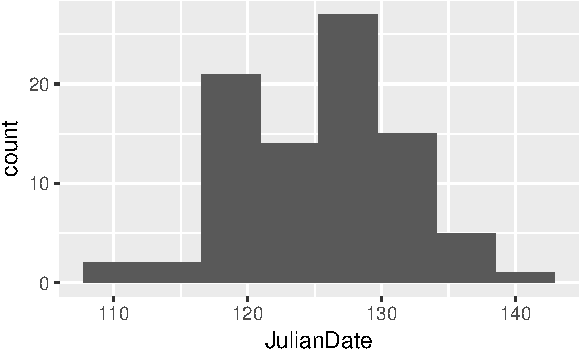
\includegraphics{03-data-summaries_files/figure-latex/unnamed-chunk-32-1}

Note that you need to type \texttt{JulianDate} exactly as it appears,
capital letters and all. R is case-sensitive.

This histogram looks more or less symmetric (and, indeed, normal). I
really don't think you can justify an answer other than ``symmetric''
here. (Or ``approximately normal'': that's good too.) If your histogram
is different, say so. I think that ``hole'' in the middle is not
especially important.

We haven't done normal quantile plots yet, but looking ahead:

\begin{Shaded}
\begin{Highlighting}[]
\KeywordTok{ggplot}\NormalTok{(nenana, }\KeywordTok{aes}\NormalTok{(}\DataTypeTok{sample =}\NormalTok{ JulianDate)) }\OperatorTok{+}\StringTok{ }\KeywordTok{stat_qq}\NormalTok{() }\OperatorTok{+}\StringTok{ }
\StringTok{    }\KeywordTok{stat_qq_line}\NormalTok{()}
\end{Highlighting}
\end{Shaded}

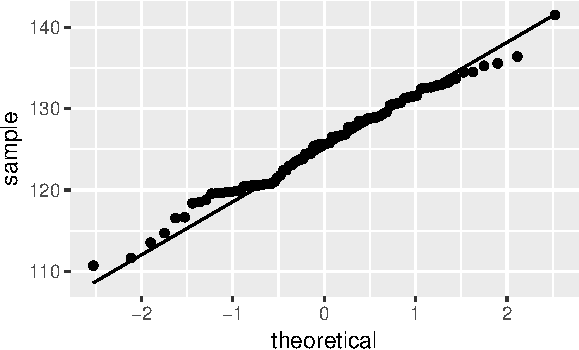
\includegraphics{03-data-summaries_files/figure-latex/unnamed-chunk-33-1}

That hugs the line pretty well, so I would call it close to
normally-distributed. It bulges away from the line because there are
more values just below 120 than you would expect for a normal. This
corresponds to the histogram bar centred just below 120 being taller
than you would have expected.
\marginnote{That is to say, the  principal deviation from normality is not the hole on the histogram, the bar centred around 123 being too short, but that the bar centred just below 120 is too *tall*.}

Extra: looking \emph{way} ahead (to almost the end of the R stuff), this
is how you handle the dates and times:

\begin{Shaded}
\begin{Highlighting}[]
\KeywordTok{library}\NormalTok{(lubridate)}
\end{Highlighting}
\end{Shaded}

\begin{verbatim}
## 
## Attaching package: 'lubridate'
\end{verbatim}

\begin{verbatim}
## The following object is masked from 'package:base':
## 
##     date
\end{verbatim}

\begin{Shaded}
\begin{Highlighting}[]
\NormalTok{nenana }\OperatorTok\StringTok{ }\KeywordTok{mutate}\NormalTok{(}\DataTypeTok{longdt =} \KeywordTok{str_c}\NormalTok{(Year, }\StringTok{" "}\NormalTok{, }\StringTok{`}\DataTypeTok{Date&Time}\StringTok{`}\NormalTok{)) }\OperatorTok\StringTok{ }
\StringTok{    }\KeywordTok{mutate}\NormalTok{(}\DataTypeTok{datetime =} \KeywordTok{ymd_hm}\NormalTok{(longdt, }\DataTypeTok{tz =} \StringTok{"America/Anchorage"}\NormalTok{))}
\end{Highlighting}
\end{Shaded}

\begin{verbatim}
## # A tibble: 87 x 5
##     Year JulianDate `Date&Time` longdt
##    <int>      <dbl> <chr>       <chr> 
##  1  1917       120. April 30 a~ 1917 ~
##  2  1918       131. May 11 at ~ 1918 ~
##  3  1919       124. May 3 at 2~ 1919 ~
##  4  1920       132. May 11 at ~ 1920 ~
##  5  1921       131. May 11 at ~ 1921 ~
##  6  1922       133. May 12 at ~ 1922 ~
##  7  1923       129. May 9 at 2~ 1923 ~
##  8  1924       133. May 11 at ~ 1924 ~
##  9  1925       128. May 7 at 6~ 1925 ~
## 10  1926       117. April 26 a~ 1926 ~
## # ... with 77 more rows, and 1 more
## #   variable: datetime <dttm>
\end{verbatim}

I am not doing any further analysis with these, so just displaying them
is good.

I have to do a preliminary step to get the date-times \emph{with} their
year in one place. \texttt{str\_c} glues pieces of text together: in
this case, the year, a space, and then the rest of the
\texttt{Date\&Time}. I stored this in \texttt{longdt}. The second
\texttt{mutate} is the business end of it: \texttt{ymd\_hm} takes a
piece of text containing a year, month (by name or number), day, hours,
minutes \emph{in that order}, and extracts those things from it, storing
the whole thing as an R date-time. Note that the AM/PM was handled
properly. The benefit of doing that is we can extract anything from the
dates, such as the month or day of week, or take differences between the
dates. Or even check that the Julian dates were calculated correctly
(the \texttt{lubridate} function is called \texttt{yday} for ``day of
year''):

\begin{Shaded}
\begin{Highlighting}[]
\NormalTok{nenana2 <-}\StringTok{ }\NormalTok{nenana }\OperatorTok\StringTok{ }\KeywordTok{mutate}\NormalTok{(}\DataTypeTok{longdt =} \KeywordTok{str_c}\NormalTok{(Year, }
    \StringTok{" "}\NormalTok{, }\StringTok{`}\DataTypeTok{Date&Time}\StringTok{`}\NormalTok{)) }\OperatorTok\StringTok{ }\KeywordTok{mutate}\NormalTok{(}\DataTypeTok{datetime =} \KeywordTok{ymd_hm}\NormalTok{(longdt, }
    \DataTypeTok{tz =} \StringTok{"America/Anchorage"}\NormalTok{)) }\OperatorTok\StringTok{ }\KeywordTok{mutate}\NormalTok{(}\DataTypeTok{jd =} \KeywordTok{yday}\NormalTok{(datetime))}
\NormalTok{nenana2 }\OperatorTok\StringTok{ }\KeywordTok{select}\NormalTok{(JulianDate, jd, datetime)}
\end{Highlighting}
\end{Shaded}

\begin{verbatim}
## # A tibble: 87 x 3
##    JulianDate    jd datetime           
##         <dbl> <dbl> <dttm>             
##  1       120.   120 1917-04-30 11:30:00
##  2       131.   131 1918-05-11 09:33:00
##  3       124.   123 1919-05-03 14:33:00
##  4       132.   132 1920-05-11 10:46:00
##  5       131.   131 1921-05-11 06:42:00
##  6       133.   132 1922-05-12 13:20:00
##  7       129.   129 1923-05-09 02:00:00
##  8       133.   132 1924-05-11 15:10:00
##  9       128.   127 1925-05-07 18:32:00
## 10       117.   116 1926-04-26 16:03:00
## # ... with 77 more rows
\end{verbatim}

Hmm, some of those are off by one. What do the off-by-one ones have in
common? Let's look at more of them. \texttt{round} rounds off to the
nearest integer (since these are actually decimal numbers):

\begin{Shaded}
\begin{Highlighting}[]
\NormalTok{nenana2 }\OperatorTok\StringTok{ }\KeywordTok{filter}\NormalTok{(}\KeywordTok{round}\NormalTok{(JulianDate) }\OperatorTok{!=}\StringTok{ }\KeywordTok{round}\NormalTok{(jd)) }\OperatorTok\StringTok{ }
\StringTok{    }\KeywordTok{select}\NormalTok{(JulianDate, jd, datetime)}
\end{Highlighting}
\end{Shaded}

\begin{verbatim}
## # A tibble: 61 x 3
##    JulianDate    jd datetime           
##         <dbl> <dbl> <dttm>             
##  1       124.   123 1919-05-03 14:33:00
##  2       133.   132 1922-05-12 13:20:00
##  3       133.   132 1924-05-11 15:10:00
##  4       128.   127 1925-05-07 18:32:00
##  5       117.   116 1926-04-26 16:03:00
##  6       128.   127 1928-05-06 16:25:00
##  7       126.   125 1929-05-05 15:41:00
##  8       129.   128 1930-05-08 19:03:00
##  9       129.   128 1933-05-08 19:30:00
## 10       121.   120 1934-04-30 14:07:00
## # ... with 51 more rows
\end{verbatim}

The ones shown here are all \emph{after noon}, and the Julian date in
the data file appears as one more than the one calculated by
\texttt{lubridate}. What has actually happened is a quirk of how tibbles
are displayed: they show 3 significant digits, \emph{rounded}. The
Julian dates given by \texttt{yday} are the whole-number part, so the
ones in the data value are that plus more than 0.5, which will round
\emph{up}. The first line of code below displays 6 significant digits
rather than only three:

\begin{Shaded}
\begin{Highlighting}[]
\KeywordTok{options}\NormalTok{(}\DataTypeTok{pillar.sigfig =} \DecValTok{6}\NormalTok{)}
\NormalTok{nenana2 }\OperatorTok\StringTok{ }\KeywordTok{filter}\NormalTok{(}\KeywordTok{round}\NormalTok{(JulianDate) }\OperatorTok{!=}\StringTok{ }\KeywordTok{round}\NormalTok{(jd)) }\OperatorTok\StringTok{ }
\StringTok{    }\KeywordTok{select}\NormalTok{(JulianDate, jd, datetime)}
\end{Highlighting}
\end{Shaded}

\begin{verbatim}
## # A tibble: 61 x 3
##    JulianDate    jd datetime           
##         <dbl> <dbl> <dttm>             
##  1    123.607   123 1919-05-03 14:33:00
##  2    132.556   132 1922-05-12 13:20:00
##  3    132.632   132 1924-05-11 15:10:00
##  4    127.773   127 1925-05-07 18:32:00
##  5    116.669   116 1926-04-26 16:03:00
##  6    127.684   127 1928-05-06 16:25:00
##  7    125.654   125 1929-05-05 15:41:00
##  8    128.794   128 1930-05-08 19:03:00
##  9    128.813   128 1933-05-08 19:30:00
## 10    120.588   120 1934-04-30 14:07:00
## # ... with 51 more rows
\end{verbatim}

Displaying more decimals shows that I was right: \texttt{jd} is (to this
accuracy) a whole number, but \texttt{JulianDate} is a decimal with
fractional part greater than 0.50.

Now I have to turn the extra signficant digits off:

\begin{Shaded}
\begin{Highlighting}[]
\KeywordTok{options}\NormalTok{(}\DataTypeTok{pillar.sigfig =} \DecValTok{3}\NormalTok{)}
\end{Highlighting}
\end{Shaded}

\begin{enumerate}
\def\labelenumi{(\alph{enumi})}
\setcounter{enumi}{3}
\tightlist
\item
  Plot \texttt{JulianDate} against \texttt{Year} on a scatterplot. What
  recent trends, if any, do you see? Comment briefly.
\end{enumerate}

Solution

\texttt{geom\_point}:

\begin{Shaded}
\begin{Highlighting}[]
\KeywordTok{ggplot}\NormalTok{(nenana, }\KeywordTok{aes}\NormalTok{(}\DataTypeTok{x =}\NormalTok{ Year, }\DataTypeTok{y =}\NormalTok{ JulianDate)) }\OperatorTok{+}\StringTok{ }
\StringTok{    }\KeywordTok{geom_point}\NormalTok{()}
\end{Highlighting}
\end{Shaded}

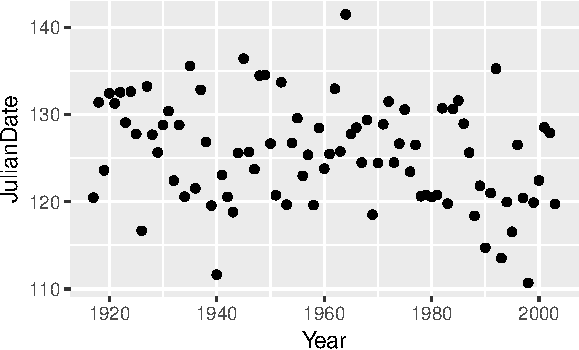
\includegraphics{03-data-summaries_files/figure-latex/unnamed-chunk-39-1}

This is actually a small-but-real downward trend, especially since about
1960, but the large amount of variability makes it hard to see, so I'm
good with either ``no trend'' or ``weak downward trend'' or anything
roughly like that. There is definitely not much trend before 1960, but
most of the really early break-ups (less than about 118) have been since
about 1990.

You can even add to the \texttt{ggplot}, by putting a smooth trend on
it:

\begin{Shaded}
\begin{Highlighting}[]
\KeywordTok{ggplot}\NormalTok{(nenana, }\KeywordTok{aes}\NormalTok{(}\DataTypeTok{x =}\NormalTok{ Year, }\DataTypeTok{y =}\NormalTok{ JulianDate)) }\OperatorTok{+}\StringTok{ }
\StringTok{    }\KeywordTok{geom_point}\NormalTok{() }\OperatorTok{+}\StringTok{ }\KeywordTok{geom_smooth}\NormalTok{()}
\end{Highlighting}
\end{Shaded}

\begin{verbatim}
## `geom_smooth()` using method = 'loess' and formula 'y ~ x'
\end{verbatim}

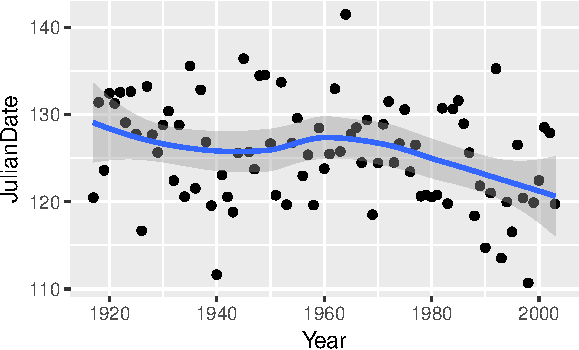
\includegraphics{03-data-summaries_files/figure-latex/unnamed-chunk-40-1}

This is R's version of a trend that is not constrained to be linear (so
that it ``lets the data speak for itself'').

Now there is something obvious to see: after about 1960, there is a
clear downward trend: the ice is breaking up earlier on average every
year. Even though there is a lot of variability, the overall trend,
viewed this way, is clear.

What does this mean, in practice? This notion of the ice melting earlier
than it used to is consistent all over the Arctic, and is one more
indication of climate change. Precisely, it is an indication that
climate change is happening, but we would have to delve further to make
any statements about the \emph{cause} of that climate change.

\hypertarget{computerized-accounting}{%
\section{Computerized accounting}\label{computerized-accounting}}

Beginning accounting students need to learn to learn to audit in a
computerized environment. A sample of beginning accounting students took
each of two tests: the Computer Attitude Scale (CAS) and the Computer
Anxiety Rating Scale (CARS). A higher score in each indicates greater
anxiety around computers. The test scores are scaled to be between 0 and
5. Also noted was each student's gender. The data are in
\url{http://www.utsc.utoronto.ca/~butler/c32/compatt.txt}. The data
values are separated by spaces.

\begin{enumerate}
\def\labelenumi{(\alph{enumi})}
\tightlist
\item
  Read the data into R. Do you have what you expected? Explain briefly.
\end{enumerate}

Solution

Read in and display the data. This, I think, is the easiest way.

\begin{Shaded}
\begin{Highlighting}[]
\NormalTok{url =}\StringTok{ "http://www.utsc.utoronto.ca/~butler/c32/compatt.txt"}
\NormalTok{anxiety =}\StringTok{ }\KeywordTok{read_delim}\NormalTok{(url, }\StringTok{" "}\NormalTok{)}
\end{Highlighting}
\end{Shaded}

\begin{verbatim}
## Parsed with column specification:
## cols(
##   gender = col_character(),
##   CAS = col_double(),
##   CARS = col_double()
## )
\end{verbatim}

\begin{Shaded}
\begin{Highlighting}[]
\NormalTok{anxiety}
\end{Highlighting}
\end{Shaded}

\begin{verbatim}
## # A tibble: 35 x 3
##    gender   CAS  CARS
##    <chr>  <dbl> <dbl>
##  1 female  2.85  2.9 
##  2 male    2.6   2.32
##  3 female  2.2   1   
##  4 male    2.65  2.58
##  5 male    2.6   2.58
##  6 male    3.2   3.05
##  7 male    3.65  3.74
##  8 female  2.55  1.9 
##  9 male    3.15  3.32
## 10 male    2.8   2.74
## # ... with 25 more rows
\end{verbatim}

There is a total of 35 students with a CAS score, a CARS score and a
gender recorded for each. This is in line with what I was expecting.
(You can also note that the genders appear to be a mixture of males and
females.)

\begin{enumerate}
\def\labelenumi{(\alph{enumi})}
\setcounter{enumi}{1}
\tightlist
\item
  How many males and females were there in the sample?
\end{enumerate}

Solution

Most easily \texttt{count}:

\begin{Shaded}
\begin{Highlighting}[]
\NormalTok{anxiety }\OperatorTok\StringTok{ }\KeywordTok{count}\NormalTok{(gender)}
\end{Highlighting}
\end{Shaded}

\begin{verbatim}
## # A tibble: 2 x 2
##   gender     n
##   <chr>  <int>
## 1 female    15
## 2 male      20
\end{verbatim}

This also works (and is therefore good):

\begin{Shaded}
\begin{Highlighting}[]
\NormalTok{anxiety }\OperatorTok\StringTok{ }\KeywordTok{group_by}\NormalTok{(gender) }\OperatorTok\StringTok{ }\KeywordTok{summarize}\NormalTok{(}\DataTypeTok{count =} \KeywordTok{n}\NormalTok{())}
\end{Highlighting}
\end{Shaded}

\begin{verbatim}
## # A tibble: 2 x 2
##   gender count
##   <chr>  <int>
## 1 female    15
## 2 male      20
\end{verbatim}

I want you to use R to do the counting (that is, don't just list out the
whole data set with \texttt{print(n=Inf)} and count the males and
females yourself). This is because you might have thousands of data
values and you need to learn how to get R (or, later, SAS) to count them
for you.

15 females and 20 males, \emph{which you should say}. I made a point of
\emph{not} saying that it is enough to get the output with the answers
on it, so you need to tell me what the answer is.

\begin{enumerate}
\def\labelenumi{(\alph{enumi})}
\setcounter{enumi}{2}
\tightlist
\item
  Do the CAS scores tend to be higher for females or for males? Draw a
  suitable graph to help you decide, and come to a conclusion.
\end{enumerate}

Solution

Gender is categorical and CAS score is quantitative, so a boxplot would
appear to be the thing:

\begin{Shaded}
\begin{Highlighting}[]
\KeywordTok{ggplot}\NormalTok{(anxiety, }\KeywordTok{aes}\NormalTok{(}\DataTypeTok{x =}\NormalTok{ gender, }\DataTypeTok{y =}\NormalTok{ CAS)) }\OperatorTok{+}\StringTok{ }\KeywordTok{geom_boxplot}\NormalTok{()}
\end{Highlighting}
\end{Shaded}

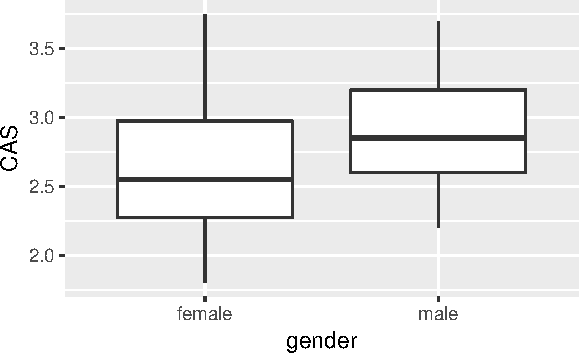
\includegraphics{03-data-summaries_files/figure-latex/unnamed-chunk-44-1}

The median for males is slightly higher, so male accountants are more
anxious around computers than female accountants are.

If you wish, side-by-side (or, better, above-and-below) histograms would
also work:

\begin{Shaded}
\begin{Highlighting}[]
\KeywordTok{ggplot}\NormalTok{(anxiety, }\KeywordTok{aes}\NormalTok{(}\DataTypeTok{x =}\NormalTok{ CAS)) }\OperatorTok{+}\StringTok{ }\KeywordTok{geom_histogram}\NormalTok{(}\DataTypeTok{bins =} \DecValTok{6}\NormalTok{) }\OperatorTok{+}\StringTok{ }
\StringTok{    }\KeywordTok{facet_wrap}\NormalTok{(}\OperatorTok{~}\NormalTok{gender, }\DataTypeTok{ncol =} \DecValTok{1}\NormalTok{)}
\end{Highlighting}
\end{Shaded}

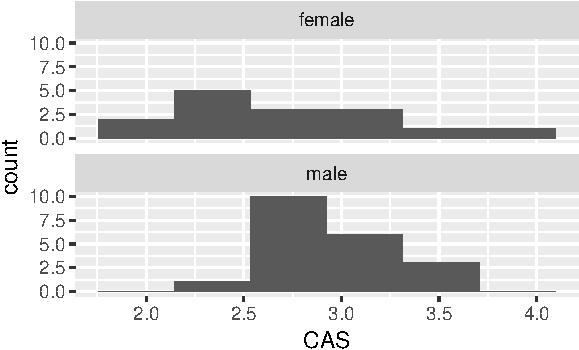
\includegraphics{03-data-summaries_files/figure-latex/unnamed-chunk-45-1}

If you go this way, you have to make a call about where the centres of
the histograms are. I guess the male one is slightly further to the
right, but it's not so easy to tell. (Make a call.)

\begin{enumerate}
\def\labelenumi{(\alph{enumi})}
\setcounter{enumi}{3}
\tightlist
\item
  Find the median CAS scores for each gender. Does this support what you
  saw on your plot? Explain briefly.
\end{enumerate}

Solution

Group-by and summarize:

\begin{Shaded}
\begin{Highlighting}[]
\NormalTok{anxiety }\OperatorTok\StringTok{ }\KeywordTok{group_by}\NormalTok{(gender) }\OperatorTok\StringTok{ }\KeywordTok{summarize}\NormalTok{(}\DataTypeTok{med =} \KeywordTok{median}\NormalTok{(CAS))}
\end{Highlighting}
\end{Shaded}

\begin{verbatim}
## # A tibble: 2 x 2
##   gender   med
##   <chr>  <dbl>
## 1 female  2.55
## 2 male    2.85
\end{verbatim}

The median is a bit higher for males, which is what I got on my boxplot
(and is apparently the same thing as is on the histograms, but it's
harder to be sure there).

\begin{enumerate}
\def\labelenumi{(\alph{enumi})}
\setcounter{enumi}{4}
\tightlist
\item
  Find the mean and standard deviation of both CAS and CARS scores (for
  all the students combined, ie.~not separated by gender) \emph{without}
  naming those columns explicitly.
\end{enumerate}

Solution

Without naming them explicitly means using some other way to pick them
out of the data frame, either \texttt{summarize\textbackslash{}\_if} or
\texttt{summarize\textbackslash{}\_at}. To do it the first way, ask what
these two columns have in common: they are the only two numeric
(quantitative) columns:

\begin{Shaded}
\begin{Highlighting}[]
\NormalTok{anxiety }\OperatorTok\StringTok{ }\KeywordTok{summarize_if}\NormalTok{(is.numeric, }\KeywordTok{funs}\NormalTok{(mean, }
\NormalTok{    sd))}
\end{Highlighting}
\end{Shaded}

\begin{verbatim}
## # A tibble: 1 x 4
##   CAS_mean CARS_mean CAS_sd CARS_sd
##      <dbl>     <dbl>  <dbl>   <dbl>
## 1     2.82      2.77  0.484   0.671
\end{verbatim}

Or the second way, asking yourself what the \emph{names} of those
columns have in common: they start with C and the gender column doesn't:

\begin{Shaded}
\begin{Highlighting}[]
\NormalTok{anxiety }\OperatorTok\StringTok{ }\KeywordTok{summarize_at}\NormalTok{(}\KeywordTok{vars}\NormalTok{(}\KeywordTok{starts_with}\NormalTok{(}\StringTok{"C"}\NormalTok{)), }
    \KeywordTok{funs}\NormalTok{(mean, sd))}
\end{Highlighting}
\end{Shaded}

\begin{verbatim}
## # A tibble: 1 x 4
##   CAS_mean CARS_mean CAS_sd CARS_sd
##      <dbl>     <dbl>  <dbl>   <dbl>
## 1     2.82      2.77  0.484   0.671
\end{verbatim}

Either of these is good, or anything equivalent (like noting that the
two anxiety scales both \texttt{ends\textbackslash{}\_with} S):

\begin{Shaded}
\begin{Highlighting}[]
\NormalTok{anxiety }\OperatorTok\StringTok{ }\KeywordTok{summarize_at}\NormalTok{(}\KeywordTok{vars}\NormalTok{(}\KeywordTok{ends_with}\NormalTok{(}\StringTok{"S"}\NormalTok{)), }
    \KeywordTok{funs}\NormalTok{(mean, sd))}
\end{Highlighting}
\end{Shaded}

\begin{verbatim}
## # A tibble: 1 x 4
##   CAS_mean CARS_mean CAS_sd CARS_sd
##      <dbl>     <dbl>  <dbl>   <dbl>
## 1     2.82      2.77  0.484   0.671
\end{verbatim}

Because I didn't say otherwise, you should tell me what the means and
SDs are, rounding off suitably: the CAS scores have mean 2.82 and SD
0.48, and the CARS scores have mean 2.77 and SD 0.67.

Yet another way to do it is to select the columns you want first (which
you can do by number so as not to name them), and then find the mean and
SD of all of them. This uses two tools that we haven't seen yet:

\begin{Shaded}
\begin{Highlighting}[]
\NormalTok{anxiety }\OperatorTok\StringTok{ }\KeywordTok{select}\NormalTok{(}\DecValTok{2}\OperatorTok{:}\DecValTok{3}\NormalTok{) }\OperatorTok\StringTok{ }\KeywordTok{summarize_all}\NormalTok{(}\KeywordTok{funs}\NormalTok{(mean, }
\NormalTok{    sd))}
\end{Highlighting}
\end{Shaded}

\begin{verbatim}
## # A tibble: 1 x 4
##   CAS_mean CARS_mean CAS_sd CARS_sd
##      <dbl>     <dbl>  <dbl>   <dbl>
## 1     2.82      2.77  0.484   0.671
\end{verbatim}

This doesn't work:

\begin{Shaded}
\begin{Highlighting}[]
\KeywordTok{summary}\NormalTok{(anxiety)}
\end{Highlighting}
\end{Shaded}

\begin{verbatim}
##     gender               CAS       
##  Length:35          Min.   :1.800  
##  Class :character   1st Qu.:2.575  
##  Mode  :character   Median :2.800  
##                     Mean   :2.816  
##                     3rd Qu.:3.150  
##                     Max.   :3.750  
##       CARS      
##  Min.   :1.000  
##  1st Qu.:2.445  
##  Median :2.790  
##  Mean   :2.771  
##  3rd Qu.:3.290  
##  Max.   :4.000
\end{verbatim}

because, although it gets the means, it does not get the standard
deviations. (I added the SD to the original question to make you find a
way other than this.)

In summary, find a way to get those answers without naming those columns
in your code, and I'm good.

In case you were wondering about how to do this separately by gender,
well, put the \texttt{group\textbackslash{}\_by} in like you did before:

\begin{Shaded}
\begin{Highlighting}[]
\NormalTok{anxiety }\OperatorTok\StringTok{ }\KeywordTok{group_by}\NormalTok{(gender) }\OperatorTok\StringTok{ }\KeywordTok{summarize_if}\NormalTok{(is.numeric, }
    \KeywordTok{funs}\NormalTok{(mean, sd))}
\end{Highlighting}
\end{Shaded}

\begin{verbatim}
## # A tibble: 2 x 5
##   gender CAS_mean CARS_mean CAS_sd CARS_sd
##   <chr>     <dbl>     <dbl>  <dbl>   <dbl>
## 1 female     2.64      2.51  0.554   0.773
## 2 male       2.94      2.96  0.390   0.525
\end{verbatim}

or

\begin{Shaded}
\begin{Highlighting}[]
\NormalTok{anxiety }\OperatorTok\StringTok{ }\KeywordTok{group_by}\NormalTok{(gender) }\OperatorTok\StringTok{ }\KeywordTok{summarize_at}\NormalTok{(}\KeywordTok{vars}\NormalTok{(}\KeywordTok{starts_with}\NormalTok{(}\StringTok{"C"}\NormalTok{)), }
    \KeywordTok{funs}\NormalTok{(mean, sd))}
\end{Highlighting}
\end{Shaded}

\begin{verbatim}
## # A tibble: 2 x 5
##   gender CAS_mean CARS_mean CAS_sd CARS_sd
##   <chr>     <dbl>     <dbl>  <dbl>   <dbl>
## 1 female     2.64      2.51  0.554   0.773
## 2 male       2.94      2.96  0.390   0.525
\end{verbatim}

The male means are slightly higher on both tests, but the male standard
deviations are a little smaller. You might be wondering whether the test
scores are related. They are both quantitative, so the obvious way to
find out is a scatterplot:

\begin{Shaded}
\begin{Highlighting}[]
\KeywordTok{ggplot}\NormalTok{(anxiety, }\KeywordTok{aes}\NormalTok{(}\DataTypeTok{x =}\NormalTok{ CAS, }\DataTypeTok{y =}\NormalTok{ CARS)) }\OperatorTok{+}\StringTok{ }\KeywordTok{geom_point}\NormalTok{()}
\end{Highlighting}
\end{Shaded}

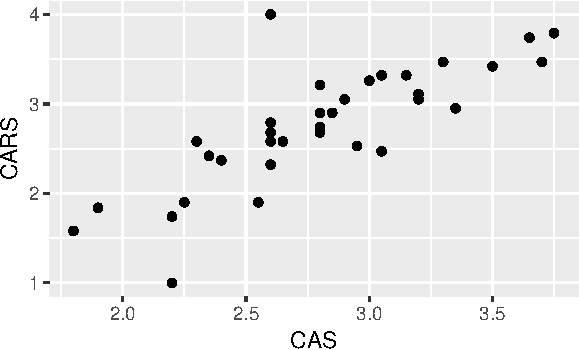
\includegraphics{03-data-summaries_files/figure-latex/unnamed-chunk-54-1}

The two variables can be on either axis, since there is no obvious
response or explanatory variable. A higher score on one scale goes with
a higher score on the other, suggesting that the two scales are
measuring the same thing.

This plot mixes up the males and females, so you might like to
distinguish them, which goes like this:

\begin{Shaded}
\begin{Highlighting}[]
\KeywordTok{ggplot}\NormalTok{(anxiety, }\KeywordTok{aes}\NormalTok{(}\DataTypeTok{x =}\NormalTok{ CAS, }\DataTypeTok{y =}\NormalTok{ CARS, }\DataTypeTok{colour =}\NormalTok{ gender)) }\OperatorTok{+}\StringTok{ }
\StringTok{    }\KeywordTok{geom_point}\NormalTok{()}
\end{Highlighting}
\end{Shaded}

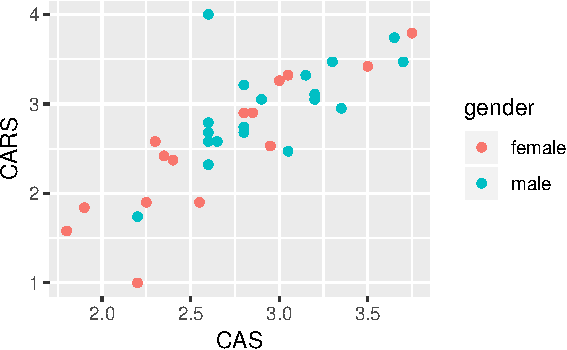
\includegraphics{03-data-summaries_files/figure-latex/unnamed-chunk-55-1}

There is a slight (but only slight) tendency for the males to be up and
to the right, and for the females to be down and to the left. This is
about what you would expect, given that the male means are slightly
bigger on both scores, but the difference in means is not that big
compared to the SD.

\hypertarget{test-scores-in-two-classes}{%
\section{Test scores in two classes}\label{test-scores-in-two-classes}}

Open R Studio. Create a new Text File by selecting File, New File and
Text File. You should see a new empty, untitled window appear at the top
left. In that window, type or copy the data below (which are scores on a
test for students in two different classes):

\begin{verbatim}

class score
ken 78
ken 62
ken 59
ken 69
ken 81
thomas 83
thomas 77
thomas 63
thomas 61
thomas 79
thomas 72
\end{verbatim}

Save the file, using a filename of your choice (with, perhaps, extension
\texttt{.txt}). Or, if you prefer, use the one at
\href{http://www.utsc.utoronto.ca/~butler/d29/marks.txt}{link}.

\begin{enumerate}
\def\labelenumi{(\alph{enumi})}
\tightlist
\item
  Read the data into a data frame called \texttt{marks}, using
  \texttt{read\_delim}, and list the data frame (by typing its name) to
  confirm that you read the data values properly. Note that the top line
  of the data file contains the names of the variables, as it ought to.
\end{enumerate}

Solution

I was lazy and used the one on the web, the values being separated
(``delimited'') by exactly one space:

\begin{Shaded}
\begin{Highlighting}[]
\NormalTok{my_url =}\StringTok{ "http://www.utsc.utoronto.ca/~butler/d29/marks.txt"}
\NormalTok{marks =}\StringTok{ }\KeywordTok{read_delim}\NormalTok{(my_url, }\StringTok{" "}\NormalTok{)}
\end{Highlighting}
\end{Shaded}

\begin{verbatim}
## Parsed with column specification:
## cols(
##   class = col_character(),
##   score = col_integer()
## )
\end{verbatim}

\begin{Shaded}
\begin{Highlighting}[]
\NormalTok{marks}
\end{Highlighting}
\end{Shaded}

\begin{verbatim}
## # A tibble: 11 x 2
##    class  score
##    <chr>  <int>
##  1 ken       78
##  2 ken       62
##  3 ken       59
##  4 ken       69
##  5 ken       81
##  6 thomas    83
##  7 thomas    77
##  8 thomas    63
##  9 thomas    61
## 10 thomas    79
## 11 thomas    72
\end{verbatim}

If you copied and pasted, or typed in, the data values yourself, use the
local file name (such as \texttt{marks.txt}) in place of the URL.

Extra: in the old days, when we used \texttt{read.table} (which actually
also works here), we needed to also say \texttt{header=T} to note that
the top line of the data file was variable names. With
\texttt{read\_delim}, that's the default, and if the top line is
\emph{not} variable names, that's when you have to say so. If I cheat,
by skipping the first line and saying that I then have no column names,
I get:

\begin{Shaded}
\begin{Highlighting}[]
\KeywordTok{read_delim}\NormalTok{(my_url, }\StringTok{" "}\NormalTok{, }\DataTypeTok{col_names =}\NormalTok{ F, }\DataTypeTok{skip =} \DecValTok{1}\NormalTok{)}
\end{Highlighting}
\end{Shaded}

\begin{verbatim}
## Parsed with column specification:
## cols(
##   X1 = col_character(),
##   X2 = col_integer()
## )
\end{verbatim}

\begin{verbatim}
## # A tibble: 11 x 2
##    X1        X2
##    <chr>  <int>
##  1 ken       78
##  2 ken       62
##  3 ken       59
##  4 ken       69
##  5 ken       81
##  6 thomas    83
##  7 thomas    77
##  8 thomas    63
##  9 thomas    61
## 10 thomas    79
## 11 thomas    72
\end{verbatim}

Column names are supplied (\texttt{X1} and \texttt{X2}). I could also
supply my own column names, in which case the file needs not to have
any, so I need the \texttt{skip} again:

\begin{Shaded}
\begin{Highlighting}[]
\KeywordTok{read_delim}\NormalTok{(my_url, }\StringTok{" "}\NormalTok{, }\DataTypeTok{col_names =} \KeywordTok{c}\NormalTok{(}\StringTok{"instructor"}\NormalTok{, }
    \StringTok{"mark"}\NormalTok{), }\DataTypeTok{skip =} \DecValTok{1}\NormalTok{)}
\end{Highlighting}
\end{Shaded}

\begin{verbatim}
## Parsed with column specification:
## cols(
##   instructor = col_character(),
##   mark = col_integer()
## )
\end{verbatim}

\begin{verbatim}
## # A tibble: 11 x 2
##    instructor  mark
##    <chr>      <int>
##  1 ken           78
##  2 ken           62
##  3 ken           59
##  4 ken           69
##  5 ken           81
##  6 thomas        83
##  7 thomas        77
##  8 thomas        63
##  9 thomas        61
## 10 thomas        79
## 11 thomas        72
\end{verbatim}

\begin{enumerate}
\def\labelenumi{(\alph{enumi})}
\setcounter{enumi}{1}
\tightlist
\item
  * Obtain side-by-side boxplots of the scores for each class.
\end{enumerate}

Solution

\begin{Shaded}
\begin{Highlighting}[]
\KeywordTok{library}\NormalTok{(tidyverse)}
\KeywordTok{ggplot}\NormalTok{(marks, }\KeywordTok{aes}\NormalTok{(}\DataTypeTok{x =}\NormalTok{ class, }\DataTypeTok{y =}\NormalTok{ score)) }\OperatorTok{+}\StringTok{ }\KeywordTok{geom_boxplot}\NormalTok{()}
\end{Highlighting}
\end{Shaded}

\includegraphics{03-data-summaries_files/figure-latex/paignton-1}

Remember: on a regular boxplot,
\marginnote{Boxplots can also go across the page, but for us, they don't.}
the groups go across (\(x\)), the variable measured goes up (\(y\)).

Extra: this might work:

\begin{Shaded}
\begin{Highlighting}[]
\KeywordTok{ggplot}\NormalTok{(marks, }\KeywordTok{aes}\NormalTok{(}\DataTypeTok{x =}\NormalTok{ class, }\DataTypeTok{y =}\NormalTok{ score)) }\OperatorTok{+}\StringTok{ }\KeywordTok{geom_boxplot}\NormalTok{() }\OperatorTok{+}\StringTok{ }
\StringTok{    }\KeywordTok{coord_flip}\NormalTok{()}
\end{Highlighting}
\end{Shaded}

\includegraphics{03-data-summaries_files/figure-latex/unnamed-chunk-59-1}

It does. That was a guess. So if you want sideways boxplots, this is how
you can get them. Long group names sometimes fit better on the
\(y\)-axis, in which case flipping the axes will help. (The \texttt{x}
and \texttt{y} happen \emph{before} the coordinate-flip, so they are the
same as above, not the same way they come out.)

\begin{enumerate}
\def\labelenumi{(\alph{enumi})}
\setcounter{enumi}{2}
\tightlist
\item
  Do the two classes appear to have similar or different scores, on
  average? Explain briefly.
\end{enumerate}

Solution

The median for Thomas's class appears to be quite a bit higher than for
Ken's class (the difference is actually about 6 marks). It's up to you
whether you think this is a big difference or not: I want you to have
\emph{an} opinion, but I don't mind so much what that opinion is. Having
said that the medians are quite a bit different, note that the boxes
overlap substantially, so that the \emph{distributions} of scores are
pretty similar (or, the quartiles of scores are similar, or, the IQR of
scores is similar for the two groups). If you say that, it's good, but
I'm not insisting that you do.

\begin{enumerate}
\def\labelenumi{(\alph{enumi})}
\setcounter{enumi}{3}
\tightlist
\item
  Obtain a boxplot of all the scores together, regardless of which class
  they came from.
\end{enumerate}

Solution

Replace your \(x\)-coordinate by some kind of dummy thing like
\texttt{1} (\texttt{factor(1)} also works):

\begin{Shaded}
\begin{Highlighting}[]
\KeywordTok{ggplot}\NormalTok{(marks, }\KeywordTok{aes}\NormalTok{(}\DataTypeTok{x =} \DecValTok{1}\NormalTok{, }\DataTypeTok{y =}\NormalTok{ score)) }\OperatorTok{+}\StringTok{ }\KeywordTok{geom_boxplot}\NormalTok{()}
\end{Highlighting}
\end{Shaded}

\includegraphics{03-data-summaries_files/figure-latex/torquay-1}

The \(x\)-axis is kind of dopey, so you just ignore it. It is possible
to remove it, but that is more work than it's worth, and I didn't get
rid of the ticks below:

\begin{Shaded}
\begin{Highlighting}[]
\KeywordTok{ggplot}\NormalTok{(marks, }\KeywordTok{aes}\NormalTok{(}\DataTypeTok{x =} \DecValTok{1}\NormalTok{, }\DataTypeTok{y =}\NormalTok{ score)) }\OperatorTok{+}\StringTok{ }\KeywordTok{geom_boxplot}\NormalTok{() }\OperatorTok{+}\StringTok{ }
\StringTok{    }\KeywordTok{theme}\NormalTok{(}\DataTypeTok{axis.text.x =} \KeywordTok{element_blank}\NormalTok{(), }\DataTypeTok{axis.title.x =} \KeywordTok{element_blank}\NormalTok{())}
\end{Highlighting}
\end{Shaded}

\includegraphics{03-data-summaries_files/figure-latex/unnamed-chunk-60-1}

\begin{enumerate}
\def\labelenumi{(\alph{enumi})}
\setcounter{enumi}{4}
\tightlist
\item
  Compute the median score (of all the scores together). Does this seem
  about right, looking at the boxplot? Explain briefly.
\end{enumerate}

Solution

Three ways to get the median score. I like the first one best:

\begin{Shaded}
\begin{Highlighting}[]
\NormalTok{marks }\OperatorTok\StringTok{ }\KeywordTok{summarize}\NormalTok{(}\DataTypeTok{med =} \KeywordTok{median}\NormalTok{(score))}
\end{Highlighting}
\end{Shaded}

\begin{verbatim}
## # A tibble: 1 x 1
##     med
##   <int>
## 1    72
\end{verbatim}

\begin{Shaded}
\begin{Highlighting}[]
\KeywordTok{with}\NormalTok{(marks, }\KeywordTok{median}\NormalTok{(score))}
\end{Highlighting}
\end{Shaded}

\begin{verbatim}
## [1] 72
\end{verbatim}

\begin{Shaded}
\begin{Highlighting}[]
\KeywordTok{median}\NormalTok{(marks}\OperatorTok{$}\NormalTok{score)}
\end{Highlighting}
\end{Shaded}

\begin{verbatim}
## [1] 72
\end{verbatim}

\texttt{summarize} is the \texttt{tidyverse} ``verb'' that does what you
want here. (The same idea gets the mean score for each class, below.)

The other ways use the basic function \texttt{median}. To make that
work, you need to say that the variable \texttt{score} whose median you
want lives in the data frame \texttt{marks}. These are two ways to do
that.

Extra: if you wanted median by group, this is the approved
(\texttt{tidyverse}) way:

\begin{Shaded}
\begin{Highlighting}[]
\NormalTok{marks }\OperatorTok\StringTok{ }\KeywordTok{group_by}\NormalTok{(class) }\OperatorTok\StringTok{ }\KeywordTok{summarize}\NormalTok{(}\DataTypeTok{med =} \KeywordTok{median}\NormalTok{(score))}
\end{Highlighting}
\end{Shaded}

\begin{verbatim}
## # A tibble: 2 x 2
##   class    med
##   <chr>  <dbl>
## 1 ken     69  
## 2 thomas  74.5
\end{verbatim}

To get something by group, the extra step is \texttt{group\_by}, and
then whatever you do after that is done for \emph{each} group.

You can now go back and compare these medians with the ones on the
boxplots in (here). They should be the same. Or you can even do this:

\begin{Shaded}
\begin{Highlighting}[]
\NormalTok{marks }\OperatorTok\StringTok{ }\KeywordTok{group_by}\NormalTok{(class) }\OperatorTok\StringTok{ }\KeywordTok{summarize}\NormalTok{(}\DataTypeTok{q1 =} \KeywordTok{quantile}\NormalTok{(score, }
    \FloatTok{0.25}\NormalTok{), }\DataTypeTok{med =} \KeywordTok{median}\NormalTok{(score), }\DataTypeTok{q3 =} \KeywordTok{quantile}\NormalTok{(score, }
    \FloatTok{0.75}\NormalTok{))}
\end{Highlighting}
\end{Shaded}

\begin{verbatim}
## # A tibble: 2 x 4
##   class     q1   med    q3
##   <chr>  <dbl> <dbl> <dbl>
## 1 ken     62    69    78  
## 2 thomas  65.2  74.5  78.5
\end{verbatim}

You can calculate as many summaries as you like. These ones should match
up with the top and bottom of the boxes on the boxplots. The only
restriction is that the things on the right side of the equals should
return a \emph{single} number. If you have a function like
\texttt{quantile} without anything extra that returns more than one
number:

\begin{Shaded}
\begin{Highlighting}[]
\KeywordTok{quantile}\NormalTok{(marks}\OperatorTok{$}\NormalTok{score)}
\end{Highlighting}
\end{Shaded}

\begin{verbatim}
##   0%  25%  50%  75% 100% 
## 59.0 62.5 72.0 78.5 83.0
\end{verbatim}

you're in trouble. Only read on if you \emph{really} want to know how to
handle this. Here's step 1:

\begin{Shaded}
\begin{Highlighting}[]
\NormalTok{marks }\OperatorTok\StringTok{ }\KeywordTok{nest}\NormalTok{(}\OperatorTok{-}\NormalTok{class)}
\end{Highlighting}
\end{Shaded}

\begin{verbatim}
## # A tibble: 2 x 2
##   class  data            
##   <chr>  <list>          
## 1 ken    <tibble [5 x 1]>
## 2 thomas <tibble [6 x 1]>
\end{verbatim}

This is kind of a funky \texttt{group\_by}. The things in the
\texttt{data} column are the \emph{whole} rest of the data frame: there
were 5 students in Ken's class and 6 in Thomas's, and they each had a
\texttt{score}, so 5 or 6 rows and 1 column. The column \texttt{data} is
known in the trade as a ``list-column''.

Now, for each of those mini-data-frames, we want to calculate the
quantiles of \texttt{score}. To do that, use \texttt{map}, which is the
\texttt{tidyverse} version of ``for each'': for each of our
mini-data-frames, calculate the five-number summary of the column called
\texttt{score} in \emph{it}:

\begin{Shaded}
\begin{Highlighting}[]
\NormalTok{marks }\OperatorTok\StringTok{ }\KeywordTok{nest}\NormalTok{(}\OperatorTok{-}\NormalTok{class) }\OperatorTok\StringTok{ }\KeywordTok{mutate}\NormalTok{(}\DataTypeTok{qq =} \KeywordTok{map}\NormalTok{(data, }
    \OperatorTok{~}\KeywordTok{quantile}\NormalTok{(.}\OperatorTok{$}\NormalTok{score)))}
\end{Highlighting}
\end{Shaded}

\begin{verbatim}
## # A tibble: 2 x 3
##   class  data             qq       
##   <chr>  <list>           <list>   
## 1 ken    <tibble [5 x 1]> <dbl [5]>
## 2 thomas <tibble [6 x 1]> <dbl [5]>
\end{verbatim}

I have to be a little bit careful about which data frame I want the
\texttt{score} to come from: the ones hidden in \texttt{data}, which are
the things we're for-eaching over.

This obtains a new list-column called \texttt{qq}, with the five-number
summary for each group.
\marginnote{It's actually a  coincidence that the five-number summary and Ken's class both have  five values in them.}

Now we want to display the quantiles. This is the easiest way:

\begin{Shaded}
\begin{Highlighting}[]
\NormalTok{marks }\OperatorTok\StringTok{ }\KeywordTok{nest}\NormalTok{(}\OperatorTok{-}\NormalTok{class) }\OperatorTok\StringTok{ }\KeywordTok{mutate}\NormalTok{(}\DataTypeTok{qq =} \KeywordTok{map}\NormalTok{(data, }
    \OperatorTok{~}\KeywordTok{quantile}\NormalTok{(.}\OperatorTok{$}\NormalTok{score))) }\OperatorTok\StringTok{ }\KeywordTok{unnest}\NormalTok{(qq)}
\end{Highlighting}
\end{Shaded}

\begin{verbatim}
## # A tibble: 10 x 2
##    class     qq
##    <chr>  <dbl>
##  1 ken     59  
##  2 ken     62  
##  3 ken     69  
##  4 ken     78  
##  5 ken     81  
##  6 thomas  61  
##  7 thomas  65.2
##  8 thomas  74.5
##  9 thomas  78.5
## 10 thomas  83
\end{verbatim}

The \texttt{unnest} turns the list-column back into actual data, so we
get the five quantiles for each class.

The only thing this doesn't do is to show us which quantile is which (we
know, of course, that the first one is the minimum, the last one is the
max and the quartiles and median are in between). It would be nice to
see which is which, though. A trick to do that is to use
\texttt{enframe}, thus:

\begin{Shaded}
\begin{Highlighting}[]
\KeywordTok{quantile}\NormalTok{(marks}\OperatorTok{$}\NormalTok{score) }\OperatorTok\StringTok{ }\KeywordTok{enframe}\NormalTok{()}
\end{Highlighting}
\end{Shaded}

\begin{verbatim}
## # A tibble: 5 x 2
##   name  value
##   <chr> <dbl>
## 1 0%     59  
## 2 25%    62.5
## 3 50%    72  
## 4 75%    78.5
## 5 100%   83
\end{verbatim}

or thus:

\begin{Shaded}
\begin{Highlighting}[]
\KeywordTok{enframe}\NormalTok{(}\KeywordTok{quantile}\NormalTok{(marks}\OperatorTok{$}\NormalTok{score))}
\end{Highlighting}
\end{Shaded}

\begin{verbatim}
## # A tibble: 5 x 2
##   name  value
##   <chr> <dbl>
## 1 0%     59  
## 2 25%    62.5
## 3 50%    72  
## 4 75%    78.5
## 5 100%   83
\end{verbatim}

I don't normally like the second way with all the brackets, but we'll be
using it later.

The idea here is that the output from a quantile is a vector, but one
with ``names'', namely the percentiles themselves. \texttt{enframe}
makes a two-column data frame with the names and the values. (You can
change the names of the columns it creates, but here we'll keep track of
which is which.)

So we have a \emph{two}-column data frame with a column saying which
quantile is which. So let's rewrite our code to use this:

\begin{Shaded}
\begin{Highlighting}[]
\NormalTok{marks }\OperatorTok\StringTok{ }\KeywordTok{nest}\NormalTok{(}\OperatorTok{-}\NormalTok{class) }\OperatorTok\StringTok{ }\KeywordTok{mutate}\NormalTok{(}\DataTypeTok{qq =} \KeywordTok{map}\NormalTok{(data, }
    \OperatorTok{~}\KeywordTok{enframe}\NormalTok{((}\KeywordTok{quantile}\NormalTok{(.}\OperatorTok{$}\NormalTok{score)))))}
\end{Highlighting}
\end{Shaded}

\begin{verbatim}
## # A tibble: 2 x 3
##   class  data             qq              
##   <chr>  <list>           <list>          
## 1 ken    <tibble [5 x 1]> <tibble [5 x 2]>
## 2 thomas <tibble [6 x 1]> <tibble [5 x 2]>
\end{verbatim}

Note that the \texttt{qq} data frames in the list-column now themselves
have two columns.

And finally \texttt{unnest} \texttt{qq}:

\begin{Shaded}
\begin{Highlighting}[]
\NormalTok{marks }\OperatorTok\StringTok{ }\KeywordTok{nest}\NormalTok{(}\OperatorTok{-}\NormalTok{class) }\OperatorTok\StringTok{ }\KeywordTok{mutate}\NormalTok{(}\DataTypeTok{qq =} \KeywordTok{map}\NormalTok{(data, }
    \OperatorTok{~}\KeywordTok{enframe}\NormalTok{((}\KeywordTok{quantile}\NormalTok{(.}\OperatorTok{$}\NormalTok{score))))) }\OperatorTok\StringTok{ }\KeywordTok{unnest}\NormalTok{(qq)}
\end{Highlighting}
\end{Shaded}

\begin{verbatim}
## # A tibble: 10 x 3
##    class  name  value
##    <chr>  <chr> <dbl>
##  1 ken    0%     59  
##  2 ken    25%    62  
##  3 ken    50%    69  
##  4 ken    75%    78  
##  5 ken    100%   81  
##  6 thomas 0%     61  
##  7 thomas 25%    65.2
##  8 thomas 50%    74.5
##  9 thomas 75%    78.5
## 10 thomas 100%   83
\end{verbatim}

Success! Or even:

\begin{Shaded}
\begin{Highlighting}[]
\NormalTok{marks }\OperatorTok\StringTok{ }\KeywordTok{nest}\NormalTok{(}\OperatorTok{-}\NormalTok{class) }\OperatorTok\StringTok{ }\KeywordTok{mutate}\NormalTok{(}\DataTypeTok{qq =} \KeywordTok{map}\NormalTok{(data, }
    \OperatorTok{~}\KeywordTok{enframe}\NormalTok{((}\KeywordTok{quantile}\NormalTok{(.}\OperatorTok{$}\NormalTok{score))))) }\OperatorTok\StringTok{ }\KeywordTok{unnest}\NormalTok{(qq) }\OperatorTok\StringTok{ }
\StringTok{    }\KeywordTok{mutate}\NormalTok{(}\DataTypeTok{qn =} \KeywordTok{parse_number}\NormalTok{(name)) }\OperatorTok\StringTok{ }\KeywordTok{select}\NormalTok{(}\OperatorTok{-}\NormalTok{name) }\OperatorTok\StringTok{ }
\StringTok{    }\KeywordTok{spread}\NormalTok{(qn, value)}
\end{Highlighting}
\end{Shaded}

\begin{verbatim}
## # A tibble: 2 x 6
##   class    `0`  `25`  `50`  `75` `100`
##   <chr>  <dbl> <dbl> <dbl> <dbl> <dbl>
## 1 ken       59  62    69    78      81
## 2 thomas    61  65.2  74.5  78.5    83
\end{verbatim}

This deliberately untidies the final answer to make it nicer to look at.
(The lines before that create a numeric quantile, so that it sorts into
the right order, and then get rid of the original quantile percents.
Investigate what happens if you do a similar \texttt{spread} without
doing that.)

\hypertarget{one-sample-inference}{%
\chapter{One-sample inference}\label{one-sample-inference}}

\begin{Shaded}
\begin{Highlighting}[]
\KeywordTok{library}\NormalTok{(tidyverse)}
\end{Highlighting}
\end{Shaded}

\begin{verbatim}
## -- Attaching packages ---- tidyverse 1.2.1 --
\end{verbatim}

\begin{verbatim}
## v ggplot2 3.1.0     v purrr   0.2.5
## v tibble  1.4.2     v dplyr   0.7.8
## v tidyr   0.8.1     v stringr 1.3.1
## v readr   1.1.1     v forcats 0.3.0
\end{verbatim}

\begin{verbatim}
## -- Conflicts ------- tidyverse_conflicts() --
## x dplyr::filter() masks stats::filter()
## x dplyr::lag()    masks stats::lag()
\end{verbatim}

\hypertarget{hunter-gatherers-in-australia}{%
\section{Hunter-gatherers in
Australia}\label{hunter-gatherers-in-australia}}

A hunter-gatherer society is one where people get their food by hunting,
fishing or foraging rather than by agriculture or by raising animals.
Such societies tend to move from place to place. Anthropologists have
studied hunter-gatherer societies in forest ecosystems across the world.
The average population density of these societies is 7.38 people per 100
km\(^2\). Hunter-gatherer societies on different continents might have
different population densities, possibly because of large-scale
ecological constraints (such as resource availability), or because of
other factors, possibly social and/or historic, determining population
density.

Some hunter-gatherer societies in Australia were studied, and the
population density per 100 km\(^2\) recorded for each. The data are in
\url{http://www.utsc.utoronto.ca/~butler/c32/hg.txt}.

\begin{enumerate}
\def\labelenumi{(\alph{enumi})}
\tightlist
\item
  Read the data into R. Do you have the correct variables? How many
  hunter-gatherer societies in Australia were studied? Explain briefly.
\end{enumerate}

Solution

The data values are separated by (single) spaces, so
\texttt{read\_delim} is the thing:

\begin{Shaded}
\begin{Highlighting}[]
\NormalTok{url =}\StringTok{ "http://www.utsc.utoronto.ca/~butler/c32/hg.txt"}
\NormalTok{societies =}\StringTok{ }\KeywordTok{read_delim}\NormalTok{(url, }\StringTok{" "}\NormalTok{)}
\end{Highlighting}
\end{Shaded}

\begin{verbatim}
## Parsed with column specification:
## cols(
##   name = col_character(),
##   density = col_double()
## )
\end{verbatim}

I like to put the URL in a variable first, because if I don't, the
\texttt{read\_delim} line can be rather long. But if you want to do it
in one step, that's fine, as long as it's clear that you are doing the
right thing.

Let's look at the data frame:

\begin{Shaded}
\begin{Highlighting}[]
\NormalTok{societies}
\end{Highlighting}
\end{Shaded}

\begin{verbatim}
## # A tibble: 13 x 2
##    name       density
##    <chr>        <dbl>
##  1 jeidji       17   
##  2 kuku         50   
##  3 mamu         45   
##  4 ngatjan      59.8 
##  5 undanbi      21.7 
##  6 jinibarra    16   
##  7 ualaria       9   
##  8 barkindji    15.4 
##  9 wongaibon     5.12
## 10 jaralde      40   
## 11 tjapwurong   35   
## 12 tasmanians   13.4 
## 13 badjalang    13.4
\end{verbatim}

I have the name of each society and its population density, as promised
(so that is correct). There were 13 societies that were studied. For me,
they were all displayed. For you, you'll probably see only the first
ten, and you'll have to click Next to see the last three.

\begin{enumerate}
\def\labelenumi{(\alph{enumi})}
\setcounter{enumi}{1}
\tightlist
\item
  The question of interest is whether these Australian hunter-gatherer
  societies are like the rest of the world in terms of mean population
  density. State suitable null and alternative hypotheses. \emph{Define
  any symbols you use}: that is, if you use a symbol, you also have to
  say what it means.
\end{enumerate}

Solution

The mean for the world as a whole (``average'', as stated earlier) is
7.38. Let \(\mu\) denote the population mean for Australia (of which
these societies are a sample). Then our hypotheses are:
\[ H_0: \mu=7.38\] and \[ H_a: \mu \ne 7.38.\] There is no reason for a
one-sided alternative here, since all we are interested in is whether
Australia is different from the rest of the world. \emph{Expect to lose
a point} if you use the symbol \(\mu\) without saying what it means.

\begin{enumerate}
\def\labelenumi{(\alph{enumi})}
\setcounter{enumi}{2}
\tightlist
\item
  Test your hypotheses using a suitable test. What do you conclude, in
  the context of the data?
\end{enumerate}

Solution

A \(t\)-test, since we are testing a mean:

\begin{Shaded}
\begin{Highlighting}[]
\KeywordTok{t.test}\NormalTok{(societies}\OperatorTok{$}\NormalTok{density, }\DataTypeTok{mu =} \FloatTok{7.38}\NormalTok{)}
\end{Highlighting}
\end{Shaded}

\begin{verbatim}
## 
##  One Sample t-test
## 
## data:  societies$density
## t = 3.8627, df = 12, p-value = 0.002257
## alternative hypothesis: true mean is not equal to 7.38
## 95 percent confidence interval:
##  15.59244 36.84449
## sample estimates:
## mean of x 
##  26.21846
\end{verbatim}

The P-value is 0.0023, less than the usual \(\alpha\) of 0.05, so we
\emph{reject} the null hypothesis and conclude that the mean population
density is not equal to 7.38. That is to say, Australia is different
from the rest of the world in this sense.

As you know, ``reject the null hypothesis'' is only part of the answer,
so gets only part of the marks.

\begin{enumerate}
\def\labelenumi{(\alph{enumi})}
\setcounter{enumi}{3}
\tightlist
\item
  Do you have any doubts about the validity of your test? Explain
  briefly, using a suitable graph to support your explanation.
\end{enumerate}

Solution

The assumption behind the \(t\)-test is that the data are approximately
normal. We can assess that in several ways, but the simplest (which is
perfectly acceptable at this point) is a histogram. You'll need to pick
a suitable number of bins. This one comes from Sturges' rule:

\begin{Shaded}
\begin{Highlighting}[]
\KeywordTok{ggplot}\NormalTok{(societies, }\KeywordTok{aes}\NormalTok{(}\DataTypeTok{x =}\NormalTok{ density)) }\OperatorTok{+}\StringTok{ }\KeywordTok{geom_histogram}\NormalTok{(}\DataTypeTok{bins =} \DecValTok{5}\NormalTok{)}
\end{Highlighting}
\end{Shaded}

\includegraphics{04-one-sample-inference_files/figure-latex/unnamed-chunk-9-1}
Your conclusion might depend on how many bins you chose for your
histogram. Here's 8 bins (which is really too many with only 13
observations, but it actually shows the shape well):

\begin{Shaded}
\begin{Highlighting}[]
\KeywordTok{ggplot}\NormalTok{(societies, }\KeywordTok{aes}\NormalTok{(}\DataTypeTok{x =}\NormalTok{ density)) }\OperatorTok{+}\StringTok{ }\KeywordTok{geom_histogram}\NormalTok{(}\DataTypeTok{bins =} \DecValTok{8}\NormalTok{)}
\end{Highlighting}
\end{Shaded}

\includegraphics{04-one-sample-inference_files/figure-latex/unnamed-chunk-10-1}

or you can get a number of bins from one of the built-in functions, such
as:

\begin{Shaded}
\begin{Highlighting}[]
\NormalTok{mybins =}\StringTok{ }\KeywordTok{nclass.FD}\NormalTok{(societies}\OperatorTok{$}\NormalTok{density)}
\NormalTok{mybins}
\end{Highlighting}
\end{Shaded}

\begin{verbatim}
## [1] 3
\end{verbatim}

This one is small. The interquartile range is large and \(n\) is small,
so the binwidth will be large and therefore the number of bins will be
small.

Other choices: a one-group boxplot:

\begin{Shaded}
\begin{Highlighting}[]
\KeywordTok{ggplot}\NormalTok{(societies, }\KeywordTok{aes}\NormalTok{(}\DataTypeTok{x =} \DecValTok{1}\NormalTok{, }\DataTypeTok{y =}\NormalTok{ density)) }\OperatorTok{+}\StringTok{ }\KeywordTok{geom_boxplot}\NormalTok{()}
\end{Highlighting}
\end{Shaded}

\includegraphics{04-one-sample-inference_files/figure-latex/unnamed-chunk-12-1}

This isn't the best for assessing normality as such, but it will tell
you about lack of symmetry and outliers, which are the most important
threats to the \(t\)-test, so it's fine here. Or, a normal quantile
plot:

\begin{Shaded}
\begin{Highlighting}[]
\KeywordTok{ggplot}\NormalTok{(societies, }\KeywordTok{aes}\NormalTok{(}\DataTypeTok{sample =}\NormalTok{ density)) }\OperatorTok{+}\StringTok{ }\KeywordTok{stat_qq}\NormalTok{() }\OperatorTok{+}\StringTok{ }
\StringTok{    }\KeywordTok{stat_qq_line}\NormalTok{()}
\end{Highlighting}
\end{Shaded}

\includegraphics{04-one-sample-inference_files/figure-latex/unnamed-chunk-13-1}

This is actually the best way to assess normality, but I'm not expecting
you to use this plot here, because we may not have gotten to it in class
yet. (If you have read ahead and successfully use the plot, it's fine.)

After you have drawn your chosen plot (you need \emph{one} plot), you
need to say something about normality and thus whether you have any
doubts about the validity of your \(t\)-test. This will depend on the
graph you drew: if you think your graph is symmetric and outlier-free,
you should have no doubts about your \(t\)-test; if you think it has
something wrong with it, you should say what it is and express your
doubts. My guess is that you will think this distribution is skewed to
the right. Most of my plots are saying that.
\marginnote{The normal  quantile plot is rather interesting: it says that the uppermost  values are approximately normal, but the *smallest* eight or so  values are too bunched up to be normal. That is, normality fails not  because of the long tail on the right, but the bunching on the  left. Still right-skewed, though.}

On the website where I got these data, they were using the data as an
example for another test, precisely \emph{because} they thought the
distribution was right-skewed. Later on, we'll learn about the sign test
for the median, which I think is actually a better test here.

\hypertarget{buses-to-boulder}{%
\section{Buses to Boulder}\label{buses-to-boulder}}

A bus line operates a route from Denver to Boulder (these places are in
Colorado). The schedule says that the journey time should be 60 minutes.
11 randomly chosen journey times were recorded, and these are in the
file \href{http://www.utsc.utoronto.ca/~butler/d29/buses.txt}{link},
with journey times shown in minutes.

\begin{enumerate}
\def\labelenumi{(\alph{enumi})}
\tightlist
\item
  Read the data into R, and display the data frame that you read in.
\end{enumerate}

Solution

Since you can read the data directly from the URL, do that (if you are
online) rather than having to copy and paste and save, and then find the
file you saved. Also, there is only one column, so you can pretend that
there were multiple columns, separated by whatever you like. It's least
typing to pretend that they were separated by commas like a
\texttt{.csv} file:

\begin{Shaded}
\begin{Highlighting}[]
\NormalTok{my_url =}\StringTok{ "http://www.utsc.utoronto.ca/~butler/d29/buses.txt"}
\NormalTok{journey.times =}\StringTok{ }\KeywordTok{read_csv}\NormalTok{(my_url)}
\end{Highlighting}
\end{Shaded}

\begin{verbatim}
## Parsed with column specification:
## cols(
##   minutes = col_integer()
## )
\end{verbatim}

\begin{Shaded}
\begin{Highlighting}[]
\NormalTok{journey.times}
\end{Highlighting}
\end{Shaded}

\begin{verbatim}
## # A tibble: 11 x 1
##    minutes
##      <int>
##  1      58
##  2      61
##  3      69
##  4      62
##  5      81
##  6      54
##  7      72
##  8      71
##  9      53
## 10      54
## 11      66
\end{verbatim}

Using \texttt{read\_delim} with any delimiter (such as \texttt{"\ "})
will also work, and is thus also good.

Variable names in R can have a dot (or an underscore, but not a space)
in them. I have grown accustomed to using dots to separate words. This
works in R but not other languages, but is seen by some as
old-fashioned, with underscores being the modern way.
\marginnote{In some  languages, a dot is used to concatenate bits of text, or as a way of  calling a method on an object. But in R, a dot has no special  meaning, and is used in function names like *t.test*. Or  *read.table*. }
You can also use what is called ``camel case'' by starting each ``word''
after the first with an uppercase letter like this:

\begin{Shaded}
\begin{Highlighting}[]
\NormalTok{journeyTimes =}\StringTok{ }\KeywordTok{read_csv}\NormalTok{(my_url)}
\end{Highlighting}
\end{Shaded}

You have to get the capitalization and punctuation right when you use
your variables, no matter what they're called. In any of the cases
above, there is no variable called \texttt{journeytimes}. As Jenny Bryan
(in
\href{http://www.stat.ubc.ca/~jenny/STAT545A/block01_basicsWorkspaceWorkingDirProject.html}{link})
puts it, boldface in original: Implicit contract with the computer /
scripting language: Computer will do tedious computation for you. In
return, you will be completely precise in your instructions. Typos
matter. Case matters. \textbf{Get better at typing.}

\begin{enumerate}
\def\labelenumi{(\alph{enumi})}
\setcounter{enumi}{1}
\tightlist
\item
  Run a suitable test to see whether there is evidence that the mean
  journey time differs from 60 minutes. What do you conclude? (I want a
  conclusion that says something about journey times of buses.)
\end{enumerate}

Solution

\texttt{t.test} doesn't take a \texttt{data=} to say which data frame to
use. Wrap it in a \texttt{with}:

\begin{Shaded}
\begin{Highlighting}[]
\KeywordTok{with}\NormalTok{(journey.times, }\KeywordTok{t.test}\NormalTok{(minutes, }\DataTypeTok{mu =} \DecValTok{60}\NormalTok{))}
\end{Highlighting}
\end{Shaded}

\begin{verbatim}
## 
##  One Sample t-test
## 
## data:  minutes
## t = 1.382, df = 10, p-value = 0.1971
## alternative hypothesis: true mean is not equal to 60
## 95 percent confidence interval:
##  57.71775 69.73680
## sample estimates:
## mean of x 
##  63.72727
\end{verbatim}

We are testing that the mean journey time is 60 minutes, against the
two-sided alternative (default) that the mean is not equal to 60
minutes. The P-value, 0.1971, is a lot bigger than the usual \(\alpha\)
of 0.05, so we cannot reject the null hypothesis. That is, there is no
evidence that the mean journey time differs from 60 minutes.

As you remember, we have not proved that the mean journey time \emph{is}
60 minutes, which is what ``accepting the null hypothesis'' would be. We
have only failed to reject it, in a shoulder-shrugging kind of way:
``the mean journey time \emph{could} be 60 minutes''. The other
acceptable word is ``retain''; when you say ``we retain the null
hypothesis'', you imply something like ``we act as if the mean is 60
minutes, at least until we find something better.''

\begin{enumerate}
\def\labelenumi{(\alph{enumi})}
\setcounter{enumi}{2}
\tightlist
\item
  Give a 95\% confidence interval for the mean journey time. (No R code
  is needed here.)
\end{enumerate}

Solution

Just read it off from the output: 57.72 to 69.74 minutes.

\begin{enumerate}
\def\labelenumi{(\alph{enumi})}
\setcounter{enumi}{3}
\tightlist
\item
  Do you draw consistent conclusions from your test and confidence
  interval? Explain briefly.
\end{enumerate}

Solution

The test said that we should not reject a mean of 60 minutes. The
confidence interval says that 60 minutes is inside the interval of
plausible values for the population mean, which is another way of saying
the same thing. (If we had rejected 60 as a mean, 60 would have been
\emph{outside} the confidence interval.)

\begin{enumerate}
\def\labelenumi{(\alph{enumi})}
\setcounter{enumi}{4}
\tightlist
\item
  Draw a boxplot of the journey times. Do you see a reason to doubt the
  test that you did above?
\end{enumerate}

Solution

The grouping variable is a ``nothing'' as in the Ken and Thomas question
(part (d)):

\begin{Shaded}
\begin{Highlighting}[]
\KeywordTok{ggplot}\NormalTok{(journey.times, }\KeywordTok{aes}\NormalTok{(}\DataTypeTok{x =} \DecValTok{1}\NormalTok{, }\DataTypeTok{y =}\NormalTok{ minutes)) }\OperatorTok{+}\StringTok{ }
\StringTok{    }\KeywordTok{geom_boxplot}\NormalTok{()}
\end{Highlighting}
\end{Shaded}

\includegraphics{04-one-sample-inference_files/figure-latex/brixham-1}

The assumption behind the \(t\)-test is that the population from which
the data come has a normal distribution: ie.~symmetric with no outliers.
A small sample (here we have 11 values) even from a normal distribution
might look quite non-normal (as in Assignment 0 from last week), so I am
not hugely concerned by this boxplot. However, it's perfectly all right
to say that this distribution is skewed, and therefore we should doubt
the \(t\)-test, because the upper whisker is longer than the lower one.
In fact, the topmost value is very nearly an outlier:
\marginnote{Whether you think it is or not may depend on how  many bins you have on your histogram. With 5 bins it looks like an  outlier, but with 6 it does not. Try it and see.}

\begin{Shaded}
\begin{Highlighting}[]
\KeywordTok{ggplot}\NormalTok{(journey.times, }\KeywordTok{aes}\NormalTok{(}\DataTypeTok{x =}\NormalTok{ minutes)) }\OperatorTok{+}\StringTok{ }\KeywordTok{geom_histogram}\NormalTok{(}\DataTypeTok{bins =} \DecValTok{5}\NormalTok{)}
\end{Highlighting}
\end{Shaded}

\includegraphics{04-one-sample-inference_files/figure-latex/babbacombe-1}

and there might be skewness as well, so maybe I should have been
concerned.

I would be looking for some intelligent comment on the boxplot: what it
looks like vs.~what it ought to look like. I don't so much mind what
that comment is, as long as it's intelligent enough.

Perhaps I should draw a normal quantile plot:

\begin{Shaded}
\begin{Highlighting}[]
\KeywordTok{ggplot}\NormalTok{(journey.times, }\KeywordTok{aes}\NormalTok{(}\DataTypeTok{sample =}\NormalTok{ minutes)) }\OperatorTok{+}\StringTok{ }
\StringTok{    }\KeywordTok{stat_qq}\NormalTok{() }\OperatorTok{+}\StringTok{ }\KeywordTok{stat_qq_line}\NormalTok{()}
\end{Highlighting}
\end{Shaded}

\includegraphics{04-one-sample-inference_files/figure-latex/unnamed-chunk-17-1}

The normal quantile plot is saying that the problem is actually at the
\emph{bottom} of the distribution: the lowest value is not low enough,
but the highest value is actually \emph{not} too high. So this one seems
to be on the edge between OK and being right-skewed (too bunched up at
the bottom). My take is that with this small sample this is not too bad.
But you are free to disagree.

If you don't like the normality, you'd use a \emph{sign test} and test
that the \emph{median} is not 60 minutes, which you would (at my guess)
utterly fail to reject:

\begin{Shaded}
\begin{Highlighting}[]
\KeywordTok{library}\NormalTok{(smmr)}
\KeywordTok{sign_test}\NormalTok{(journey.times, minutes, }\DecValTok{60}\NormalTok{)}
\end{Highlighting}
\end{Shaded}

\begin{verbatim}
## $above_below
## below above 
##     4     7 
## 
## $p_values
##   alternative   p_value
## 1       lower 0.8867187
## 2       upper 0.2744141
## 3   two-sided 0.5488281
\end{verbatim}

\begin{Shaded}
\begin{Highlighting}[]
\KeywordTok{ci_median}\NormalTok{(journey.times, minutes)}
\end{Highlighting}
\end{Shaded}

\begin{verbatim}
## [1] 54.00195 71.99023
\end{verbatim}

and so we do. The median could easily be 60 minutes.

\hypertarget{length-of-gestation-in-north-carolina}{%
\section{Length of gestation in North
Carolina}\label{length-of-gestation-in-north-carolina}}

The data in file
\href{http://www.utsc.utoronto.ca/~butler/c32/ncbirths.csv}{link} are
about 500 randomly chosen births of babies in North Carolina. There is a
lot of information: not just the weight at birth of the baby, but
whether the baby was born prematurely, the ages of the parents, whether
the parents are married, how long (in weeks) the pregnancy lasted (this
is called the ``gestation'') and so on. We have seen these data before.

\begin{enumerate}
\def\labelenumi{(\alph{enumi})}
\tightlist
\item
  Read in the data from the file into R, bearing in mind what type of
  file it is.
\end{enumerate}

Solution

This is a \texttt{.csv} file (it came from a spreadsheet), so it needs
reading in accordingly. Work directly from the URL (rather than
downloading the file, unless you are working offline):

\begin{Shaded}
\begin{Highlighting}[]
\NormalTok{myurl =}\StringTok{ "http://www.utsc.utoronto.ca/~butler/c32/ncbirths.csv"}
\NormalTok{bw =}\StringTok{ }\KeywordTok{read_csv}\NormalTok{(myurl)}
\end{Highlighting}
\end{Shaded}

\begin{verbatim}
## Parsed with column specification:
## cols(
##   `Father Age` = col_integer(),
##   `Mother Age` = col_integer(),
##   `Weeks Gestation` = col_integer(),
##   `Pre-natal Visits` = col_integer(),
##   `Marital Status` = col_integer(),
##   `Mother Weight Gained` = col_integer(),
##   `Low Birthweight?` = col_integer(),
##   `Weight (pounds)` = col_double(),
##   `Premie?` = col_integer(),
##   `Few Visits?` = col_integer()
## )
\end{verbatim}

\begin{enumerate}
\def\labelenumi{(\alph{enumi})}
\setcounter{enumi}{1}
\tightlist
\item
  Find a 95\% confidence interval for the mean birth weight of all
  babies born in North Carolina (of which these babies are a sample). At
  the end, you should state what the confidence interval is. Giving some
  output is necessary, but \emph{not} enough by itself.
\end{enumerate}

If your variable name has a space or other special character (like a
question mark) in it, remember that you have to surround its name with
backticks, as discussed the first time we looked at these data.

Solution

This:

\begin{Shaded}
\begin{Highlighting}[]
\KeywordTok{t.test}\NormalTok{(bw}\OperatorTok{$}\StringTok{`}\DataTypeTok{Weight (pounds)}\StringTok{`}\NormalTok{)}
\end{Highlighting}
\end{Shaded}

\begin{verbatim}
## 
##  One Sample t-test
## 
## data:  bw$`Weight (pounds)`
## t = 104.94, df = 499, p-value < 2.2e-16
## alternative hypothesis: true mean is not equal to 0
## 95 percent confidence interval:
##  6.936407 7.201093
## sample estimates:
## mean of x 
##   7.06875
\end{verbatim}

or (the same, but remember to match your brackets):

\begin{Shaded}
\begin{Highlighting}[]
\KeywordTok{with}\NormalTok{(bw, }\KeywordTok{t.test}\NormalTok{(}\StringTok{`}\DataTypeTok{Weight (pounds)}\StringTok{`}\NormalTok{))}
\end{Highlighting}
\end{Shaded}

\begin{verbatim}
## 
##  One Sample t-test
## 
## data:  Weight (pounds)
## t = 104.94, df = 499, p-value < 2.2e-16
## alternative hypothesis: true mean is not equal to 0
## 95 percent confidence interval:
##  6.936407 7.201093
## sample estimates:
## mean of x 
##   7.06875
\end{verbatim}

The confidence interval goes from 6.94 to 7.20 pounds.

There is an annoyance about \texttt{t.test}. Sometimes you can use
\texttt{data=} with it, and sometimes not. When we do a two-sample
\(t\)-test later, there is a ``model formula'' with a squiggle in it,
and there we can use \texttt{data=}, but here not, so you have to use
the dollar sign or the \texttt{with} to say which data frame to get
things from. The distinction seems to be that \emph{if you are using a
model formula}, you can use \texttt{data=}, and if not, not.

This is one of those things that is a consequence of R's history. The
original \texttt{t.test} was without the model formula and thus without
the \texttt{data=}, but the model formula got ``retro-fitted'' to it
later. Since the model formula comes from things like regression, where
\texttt{data=} is legit, that had to be retro-fitted as well. Or, at
least, that's my understanding.

\begin{enumerate}
\def\labelenumi{(\alph{enumi})}
\setcounter{enumi}{2}
\tightlist
\item
  Birth weights of babies born in the United States have a mean of 7.3
  pounds. Is there any evidence that babies born in North Carolina are
  less heavy on average? State appropriate hypotheses, do your test,
  obtain a P-value and state your conclusion, in terms of the original
  data.
\end{enumerate}

Solution

Let \(\mu\) be the population mean (the mean weight of all babies born
in North Carolina). Null hypothesis is \(H_0: \mu=7.3\) pounds, and the
alternative is that the mean is less: \(H_a: \mu<7.3\) pounds.

Note that I defined \(\mu\) first before I used it.

This is a one-sided alternative, which we need to feed into
\texttt{t.test}:

\begin{Shaded}
\begin{Highlighting}[]
\KeywordTok{t.test}\NormalTok{(bw}\OperatorTok{$}\StringTok{`}\DataTypeTok{Weight (pounds)}\StringTok{`}\NormalTok{, }\DataTypeTok{mu =} \FloatTok{7.3}\NormalTok{, }\DataTypeTok{alternative =} \StringTok{"less"}\NormalTok{)}
\end{Highlighting}
\end{Shaded}

\begin{verbatim}
## 
##  One Sample t-test
## 
## data:  bw$`Weight (pounds)`
## t = -3.4331, df = 499, p-value =
## 0.0003232
## alternative hypothesis: true mean is less than 7.3
## 95 percent confidence interval:
##      -Inf 7.179752
## sample estimates:
## mean of x 
##   7.06875
\end{verbatim}

\$ \%\$

Or with \texttt{with}. If you see what I mean.

The P-value is 0.0003, which is \emph{less} than any \(\alpha\) we might
have chosen: we \emph{reject} the null hypothesis in favour of the
alternative, and thus we conclude that the mean birth weight of babies
in North Carolina is indeed less than 7.3 pounds.

``Reject the null hypothesis'' is \emph{not} a complete answer. You need
to say something about what rejecting the null hypothesis means \emph{in
this case}: that is, you must make a statement about birth weights of
babies.

\begin{enumerate}
\def\labelenumi{(\alph{enumi})}
\setcounter{enumi}{3}
\tightlist
\item
  The theory behind the \(t\)-test says that the distribution of birth
  weights should be (approximately) normally distributed. Obtain a
  histogram of the birth weights. Does it look approximately normal?
  Comment briefly. (You'll have to pick a number of bins for your
  histogram first. I don't mind very much what you pick, as long as it's
  not obviously too many or too few bins.)
\end{enumerate}

Solution

We did this before (and discussed the number of bins before), so I'll
just reproduce my 10-bin histogram (which is what I preferred, but this
is a matter of taste):

\begin{Shaded}
\begin{Highlighting}[]
\KeywordTok{ggplot}\NormalTok{(bw, }\KeywordTok{aes}\NormalTok{(}\DataTypeTok{x =} \StringTok{`}\DataTypeTok{Weight (pounds)}\StringTok{`}\NormalTok{)) }\OperatorTok{+}\StringTok{ }\KeywordTok{geom_histogram}\NormalTok{(}\DataTypeTok{bins =} \DecValTok{10}\NormalTok{)}
\end{Highlighting}
\end{Shaded}

\includegraphics{04-one-sample-inference_files/figure-latex/unnamed-chunk-23-1}

So, we were assessing normality. What about that?

It is mostly normal-looking, but I am suspicious about those \emph{very}
low birth weights, the ones below about 4 pounds. There are too many of
those, as I see it.

If you think this is approximately normal, you need to make some comment
along the lines of ``the shape is approximately symmetric with no
outliers''. I think my first answer is better, but this answer is worth
something, since it is a not completely unreasonable interpretation of
the histogram.

A normal quantile plot is better for assessing normality than a
histogram is, but I won't make you do one until we have seen the idea in
class. Here's the normal quantile plot for these data:

\begin{Shaded}
\begin{Highlighting}[]
\KeywordTok{ggplot}\NormalTok{(bw, }\KeywordTok{aes}\NormalTok{(}\DataTypeTok{sample =} \StringTok{`}\DataTypeTok{Weight (pounds)}\StringTok{`}\NormalTok{)) }\OperatorTok{+}\StringTok{ }
\StringTok{    }\KeywordTok{stat_qq}\NormalTok{() }\OperatorTok{+}\StringTok{ }\KeywordTok{stat_qq_line}\NormalTok{()}
\end{Highlighting}
\end{Shaded}

\includegraphics{04-one-sample-inference_files/figure-latex/unnamed-chunk-24-1}

This is rather striking: the lowest birthweights (the ones below 5
pounds or so) are \emph{way} too low for a normal distribution to apply.
The top end is fine (except perhaps for that one very heavy baby), but
there are too many low birthweights for a normal distribution to be
believable. Note how much clearer this story is than on the histogram.

Having said that, the \(t\)-test, especially with a sample size as big
as this (500), behaves \emph{very} well when the data are somewhat
non-normal (because it takes advantage of the Central Limit Theorem:
that is, it's the \emph{sampling distribution of the sample mean} whose
shape matters). So, even though the data are definitely not normal, I
wouldn't be too worried about our test.

This perhaps gives some insight as to why Freedman-Diaconis said we
should use so many bins for our histogram. We have a lot of low-end
outliers, so that the IQR is actually \emph{small} compared to the
overall spread of the data (as measured, say, by the SD or the range)
and so FD thinks we need a lot of bins to describe the shape. Sturges is
based on data being approximately normal, so it will tend to produce a
small number of bins for data that have outliers.

\hypertarget{inferring-ice-break-up-in-nenana}{%
\section{Inferring ice break-up in
Nenana}\label{inferring-ice-break-up-in-nenana}}

Nenana, Alaska, is about 50 miles west of Fairbanks. Every spring, there
is a contest in Nenana. A wooden tripod is placed on the frozen river,
and people try to guess the exact minute when the ice melts enough for
the tripod to fall through the ice. The contest started in 1917 as an
amusement for railway workers, and has taken place every year since.
Now, hundreds of thousands of people enter their guesses on the Internet
and the prize for the winner can be as much as \$300,000.

Because so much money is at stake, and because the exact same tripod is
placed at the exact same spot on the ice every year, the data are
consistent and accurate. The data are in
\href{http://www.utsc.utoronto.ca/~butler/c32/nenana.txt}{link}.

Yes, we saw these data before.

\begin{enumerate}
\def\labelenumi{(\alph{enumi})}
\tightlist
\item
  Read the data into R, as before, or use the data frame that you read
  in before. Note that the values are separated by \emph{tabs} rather
  than spaces, so you'll need an appropriate \texttt{read\_} to read it
  in.
\end{enumerate}

Solution

These are ``tab-separated values'', so \texttt{read\_tsv} is the thing,
as for the Australian athletes:

\begin{Shaded}
\begin{Highlighting}[]
\NormalTok{myurl =}\StringTok{ "http://www.utsc.utoronto.ca/~butler/c32/nenana.txt"}
\NormalTok{nenana =}\StringTok{ }\KeywordTok{read_tsv}\NormalTok{(myurl)}
\end{Highlighting}
\end{Shaded}

\begin{verbatim}
## Parsed with column specification:
## cols(
##   Year = col_integer(),
##   JulianDate = col_double(),
##   `Date&Time` = col_character()
## )
\end{verbatim}

Use whatever name you like for the data frame. One that is different
from any of the column headers is smart; then it is clear whether you
mean the whole data frame or one of its columns. \texttt{ice} or
\texttt{melt} or anything like that would also be good.

\begin{enumerate}
\def\labelenumi{(\alph{enumi})}
\setcounter{enumi}{1}
\tightlist
\item
  Obtain a 90\% confidence interval for the mean \texttt{JulianDate}.
  What interval do you get? Looking back at your histogram, do you have
  any doubts about the validity of what you have just done?
\end{enumerate}

Solution

This is a matter of using \texttt{t.test} and pulling out the interval.
Since we are looking for a non-standard interval, we have to remember
\texttt{conf.level} as the way to get the confidence level that we want.
I'm going with \texttt{with} this time, though the dollar-sign thing is
equally as good:

\begin{Shaded}
\begin{Highlighting}[]
\KeywordTok{with}\NormalTok{(nenana, }\KeywordTok{t.test}\NormalTok{(JulianDate, }\DataTypeTok{conf.level =} \FloatTok{0.9}\NormalTok{))}
\end{Highlighting}
\end{Shaded}

\begin{verbatim}
## 
##  One Sample t-test
## 
## data:  JulianDate
## t = 197.41, df = 86, p-value < 2.2e-16
## alternative hypothesis: true mean is not equal to 0
## 90 percent confidence interval:
##  124.4869 126.6018
## sample estimates:
## mean of x 
##  125.5443
\end{verbatim}

Between 124.5 and 126.6 days into the year. Converting that into
something we can understand (because I want to), there are
\(31+28+31+30=120\) days in January through April (in a non-leap year),
so this says that the mean breakup date is between about May 4 and May
6.

The \(t\)-test is based on an assumption of data coming from a normal
distribution. The histogram we made earlier looks pretty much normal, so
there are no doubts about normality and thus no doubts about the
validity of what we have done, on the evidence we have seen so far. (I
have some doubts on different grounds, based on another of the plots we
did earlier, which I'll explain later, but all I'm expecting you to do
is to look at the histogram and say ``Yep, that's normal enough''. Bear
in mind that the sample size is 87, which is large enough for the
Central Limit Theorem to be pretty helpful, so that we don't need the
data to be more than ``approximately normal'' for the sampling
distribution of the sample mean to be very close to \(t\) with the right
df.)

\begin{enumerate}
\def\labelenumi{(\alph{enumi})}
\setcounter{enumi}{2}
\tightlist
\item
  An old-timer in Nenana strokes his grey beard and says ``When I were
  young, I remember the tripod used to fall into the water around May
  10''. In a non-leap year, May 10 is Julian day 130. Test the null
  hypothesis that the mean \texttt{JulianDay} is 130, against the
  alternative that it is less. What do you conclude? What practical
  implication does that have (assuming that the old-timer has a good
  memory)?
\end{enumerate}

Solution

The test is \texttt{t.test} again, but this time we have to specify a
null mean and a direction of alternative:

\begin{Shaded}
\begin{Highlighting}[]
\KeywordTok{with}\NormalTok{(nenana, }\KeywordTok{t.test}\NormalTok{(JulianDate, }\DataTypeTok{mu =} \DecValTok{130}\NormalTok{, }\DataTypeTok{alternative =} \StringTok{"less"}\NormalTok{))}
\end{Highlighting}
\end{Shaded}

\begin{verbatim}
## 
##  One Sample t-test
## 
## data:  JulianDate
## t = -7.0063, df = 86, p-value =
## 2.575e-10
## alternative hypothesis: true mean is less than 130
## 95 percent confidence interval:
##      -Inf 126.6018
## sample estimates:
## mean of x 
##  125.5443
\end{verbatim}

For a test, look first at the P-value, which is 0.0000000002575: that is
to say, the P-value is very small, definitely smaller than 0.05 (or any
other \(\alpha\) you might have chosen). So we \emph{reject} the null
hypothesis, and conclude that the mean \texttt{JulianDate} is actually
\emph{less} than 130.

Now, this is the date on which the ice breaks up on average, and we have
concluded that it is \emph{earlier} than it used to be, since we are
assuming the old-timer's memory is correct.

This is evidence in favour of global warming; a small piece of evidence,
to be sure, but the ice is melting earlier than it used to all over the
Arctic, so it's not just in Nenana that it is happening. You don't need
to get to the ``global warming'' part, but I \emph{do} want you to
observe that the ice is breaking up earlier than it used to.

\begin{enumerate}
\def\labelenumi{(\alph{enumi})}
\setcounter{enumi}{3}
\tightlist
\item
  Plot \texttt{JulianDate} against \texttt{Year} on a scatterplot. What
  recent trends, if any, do you see? Comment briefly. (You did this
  before, but I have some extra comments on the graph this time, so feel
  free to just read this part.)
\end{enumerate}

Solution

I liked the \texttt{ggplot} with a smooth trend on it:

\begin{Shaded}
\begin{Highlighting}[]
\KeywordTok{ggplot}\NormalTok{(nenana, }\KeywordTok{aes}\NormalTok{(}\DataTypeTok{x =}\NormalTok{ Year, }\DataTypeTok{y =}\NormalTok{ JulianDate)) }\OperatorTok{+}\StringTok{ }
\StringTok{    }\KeywordTok{geom_point}\NormalTok{() }\OperatorTok{+}\StringTok{ }\KeywordTok{geom_smooth}\NormalTok{()}
\end{Highlighting}
\end{Shaded}

\begin{verbatim}
## `geom_smooth()` using method = 'loess' and formula 'y ~ x'
\end{verbatim}

\includegraphics{04-one-sample-inference_files/figure-latex/unnamed-chunk-28-1}

There was something obvious to see: after about 1960, there is a clear
downward trend: the ice is breaking up earlier on average every year.
Even though there is a lot of variability, the overall trend, viewed
this way, is clear (and consistent with the test we did earlier). Note
that the old-timer's value of 130 is the kind of \texttt{JulianDate} we
would typically observe around 1920, which would make the old-timer over
90 years old.

All right, why did I say I had some doubts earlier? Well, because of
this downward trend, the mean is not actually the same all the way
through, so it doesn't make all that much sense to estimate it, which is
what we were doing earlier by doing a confidence interval or a
hypothesis test. What would actually make more sense is to estimate the
mean \texttt{JulianDate} \emph{for a particular year}. This could be
done by a regression: predict \texttt{JulianDate} from \texttt{Year},
and then get a ``confidence interval for the mean response'' (as you
would have seen in B27 or will see in C67). The trend isn't really
linear, but is not that far off. I can modify the previous picture to
give you an idea. Putting in \texttt{method="lm"} fits a line; as we see
later, \texttt{lm} does regressions in R:

\begin{Shaded}
\begin{Highlighting}[]
\KeywordTok{ggplot}\NormalTok{(nenana, }\KeywordTok{aes}\NormalTok{(}\DataTypeTok{x =}\NormalTok{ Year, }\DataTypeTok{y =}\NormalTok{ JulianDate)) }\OperatorTok{+}\StringTok{ }
\StringTok{    }\KeywordTok{geom_point}\NormalTok{() }\OperatorTok{+}\StringTok{ }\KeywordTok{geom_smooth}\NormalTok{(}\DataTypeTok{method =} \StringTok{"lm"}\NormalTok{)}
\end{Highlighting}
\end{Shaded}

\includegraphics{04-one-sample-inference_files/figure-latex/unnamed-chunk-29-1}

Compare the confidence interval for the mean \texttt{JulianDate} in
1920: 126 to 131 (the shaded area on the graph), with 2000: 121 to 125.
A change of about 5 days over 80 years. And with the recent trend that
we saw above, it's probably changing faster than that now. Sobering
indeed.

\hypertarget{two-sample-inference}{%
\chapter{Two-sample inference}\label{two-sample-inference}}

\begin{Shaded}
\begin{Highlighting}[]
\KeywordTok{library}\NormalTok{(tidyverse)}
\end{Highlighting}
\end{Shaded}

\begin{verbatim}
## -- Attaching packages ---- tidyverse 1.2.1 --
\end{verbatim}

\begin{verbatim}
## v ggplot2 3.1.0     v purrr   0.2.5
## v tibble  1.4.2     v dplyr   0.7.8
## v tidyr   0.8.1     v stringr 1.3.1
## v readr   1.1.1     v forcats 0.3.0
\end{verbatim}

\begin{verbatim}
## -- Conflicts ------- tidyverse_conflicts() --
## x dplyr::filter() masks stats::filter()
## x dplyr::lag()    masks stats::lag()
\end{verbatim}

\hypertarget{children-and-electronic-devices}{%
\section{Children and electronic
devices}\label{children-and-electronic-devices}}

Do children (aged 8--17) spend more time on electronic devices now than
they did 10 years ago? Samples of 15 children aged 8--17 were taken in
each of two years, 1999 and 2009, and the children (with their parents'
help) were asked to keep a diary of the number of hours they spent using
electronic devices on a certain day. The data are in the file
\url{http://www.utsc.utoronto.ca/~butler/c32/pluggedin.txt}.

\begin{enumerate}
\def\labelenumi{(\alph{enumi})}
\tightlist
\item
  Read in the data and verify that you have 30 rows of data from two
  different years.
\end{enumerate}

Solution

I see this:

\begin{Shaded}
\begin{Highlighting}[]
\NormalTok{myurl =}\StringTok{ "http://www.utsc.utoronto.ca/~butler/c32/pluggedin.txt"}
\NormalTok{plugged =}\StringTok{ }\KeywordTok{read_delim}\NormalTok{(myurl, }\StringTok{" "}\NormalTok{)}
\end{Highlighting}
\end{Shaded}

\begin{verbatim}
## Parsed with column specification:
## cols(
##   year = col_integer(),
##   hours = col_integer()
## )
\end{verbatim}

\begin{Shaded}
\begin{Highlighting}[]
\NormalTok{plugged}
\end{Highlighting}
\end{Shaded}

\begin{verbatim}
## # A tibble: 30 x 2
##     year hours
##    <int> <int>
##  1  1999     4
##  2  1999     5
##  3  1999     7
##  4  1999     7
##  5  1999     5
##  6  1999     7
##  7  1999     5
##  8  1999     6
##  9  1999     5
## 10  1999     6
## # ... with 20 more rows
\end{verbatim}

I see only the first ten rows (with an indication that there are 20
more, so 30 altogether). In your notebook, it'll look a bit different:
again, you'll see the first 10 rows, but you'll see exactly how many
rows and columns there are, and there will be buttons ``Next'' and
``Previous'' to see earlier and later rows, and a little right-arrow to
see more columns to the right (to which is added a little left-arrow if
there are previous columns to scroll back to). If you want to check for
yourself that there are 30 rows, you can click Next a couple of times to
get down to row 30, and then see that the Next button cannot be clicked
again, and therefore that 30 rows is how many there are.

Or, you can summarize the years by counting how many there are of each:

\begin{Shaded}
\begin{Highlighting}[]
\NormalTok{plugged }\OperatorTok\StringTok{ }\KeywordTok{count}\NormalTok{(year)}
\end{Highlighting}
\end{Shaded}

\begin{verbatim}
## # A tibble: 2 x 2
##    year     n
##   <int> <int>
## 1  1999    15
## 2  2009    15
\end{verbatim}

or the more verbose form of the same thing:

\begin{Shaded}
\begin{Highlighting}[]
\NormalTok{plugged }\OperatorTok\StringTok{ }\KeywordTok{group_by}\NormalTok{(year) }\OperatorTok\StringTok{ }\KeywordTok{summarize}\NormalTok{(}\DataTypeTok{rows =} \KeywordTok{n}\NormalTok{())}
\end{Highlighting}
\end{Shaded}

\begin{verbatim}
## # A tibble: 2 x 2
##    year  rows
##   <int> <int>
## 1  1999    15
## 2  2009    15
\end{verbatim}

Any of those says that it looks good. 30 rows, 1999 and 2009, 15
measurements for each.

\begin{enumerate}
\def\labelenumi{(\alph{enumi})}
\setcounter{enumi}{1}
\tightlist
\item
  Draw side-by-side boxplots of the number of hours for each year.
  \texttt{year} is a numeric variable that we want to treat as a factor,
  so we need to \emph{make} it into a factor.
\end{enumerate}

Solution

\begin{Shaded}
\begin{Highlighting}[]
\KeywordTok{ggplot}\NormalTok{(plugged, }\KeywordTok{aes}\NormalTok{(}\DataTypeTok{x =} \KeywordTok{factor}\NormalTok{(year), }\DataTypeTok{y =}\NormalTok{ hours)) }\OperatorTok{+}\StringTok{ }
\StringTok{    }\KeywordTok{geom_boxplot}\NormalTok{()}
\end{Highlighting}
\end{Shaded}

\includegraphics{05-two-sample-inference_files/figure-latex/unnamed-chunk-5-1}

The \texttt{fct\_inorder} trick from assignment 1 will also work, since
the years are in the data in the order we want them to be displayed.

The median for 2009 is noticeably higher, and there is no skewness or
outliers worth worrying about.

The measurements for the two years have a very similar spread, so there
would be no problem running the pooled test here.

You might be bothered by the \texttt{factor(year)} on the \(x\)-axis. To
get around that, you can define year-as-factor \emph{first}, using
\texttt{mutate}, then feed your new column into the boxplot. That goes
like this. There is a wrinkle that I explain afterwards:

\begin{Shaded}
\begin{Highlighting}[]
\NormalTok{plugged }\OperatorTok\StringTok{ }\KeywordTok{mutate}\NormalTok{(}\DataTypeTok{the_year =} \KeywordTok{factor}\NormalTok{(year)) }\OperatorTok\StringTok{ }
\StringTok{    }\KeywordTok{ggplot}\NormalTok{(}\KeywordTok{aes}\NormalTok{(}\DataTypeTok{x =}\NormalTok{ the_year, }\DataTypeTok{y =}\NormalTok{ hours)) }\OperatorTok{+}\StringTok{ }\KeywordTok{geom_boxplot}\NormalTok{()}
\end{Highlighting}
\end{Shaded}

\includegraphics{05-two-sample-inference_files/figure-latex/unnamed-chunk-6-1}

You could even redefine \texttt{year} to be the factor version of itself
(if you don't need the year-as-number anywhere else). The wrinkle I
mentioned above is that in the \texttt{ggplot} you \emph{do
not} name the data frame first; the data frame used is the (nameless)
data frame that came out of the previous step, not \texttt{plugged} but
\texttt{plugged} with a new column \texttt{the\_year}.

Note how the \(x\)-axis now has the name of the new variable.

If you forget to make \texttt{year} into a factor, this happens:

\begin{Shaded}
\begin{Highlighting}[]
\KeywordTok{ggplot}\NormalTok{(plugged, }\KeywordTok{aes}\NormalTok{(}\DataTypeTok{x =}\NormalTok{ year, }\DataTypeTok{y =}\NormalTok{ hours)) }\OperatorTok{+}\StringTok{ }\KeywordTok{geom_boxplot}\NormalTok{()}
\end{Highlighting}
\end{Shaded}

\begin{verbatim}
## Warning: Continuous x aesthetic -- did you
## forget aes(group=...)?
\end{verbatim}

\includegraphics{05-two-sample-inference_files/figure-latex/unnamed-chunk-7-1}

You get \emph{one} boxplot, for all the hours, without distinguishing by
year, and a warning message that tries (and fails) to read our mind:
yes, we have a continuous, quantitative \texttt{x}, but
\texttt{geom\_boxplot} doesn't take a \texttt{group}.

\begin{enumerate}
\def\labelenumi{(\alph{enumi})}
\setcounter{enumi}{2}
\tightlist
\item
  Test whether the mean number of hours has \emph{increased} since
\end{enumerate}

\begin{enumerate}
\def\labelenumi{\arabic{enumi}.}
\setcounter{enumi}{1998}
\tightlist
\item
  Which test did R do?
\end{enumerate}

Solution

The hard part to remember is how you specify a one-sided test in R; it's
\texttt{alternative="less"} (rather than ``greater'') because 1999 is
``before'' 2009:

\begin{Shaded}
\begin{Highlighting}[]
\KeywordTok{t.test}\NormalTok{(hours }\OperatorTok{~}\StringTok{ }\NormalTok{year, }\DataTypeTok{data =}\NormalTok{ plugged, }\DataTypeTok{alternative =} \StringTok{"less"}\NormalTok{)}
\end{Highlighting}
\end{Shaded}

\begin{verbatim}
## 
##  Welch Two Sample t-test
## 
## data:  hours by year
## t = -3.3323, df = 24.861, p-value =
## 0.001348
## alternative hypothesis: true difference in means is less than 0
## 95 percent confidence interval:
##        -Inf -0.8121415
## sample estimates:
## mean in group 1999 mean in group 2009 
##           5.933333           7.600000
\end{verbatim}

The P-value is 0.0013. R does the Welch-Satterthwaite test by default
(the unequal-variances one). Since we didn't change that, that's what we
got. (The pooled test is below.)

This is the cleanest way to do it, because this version of
\texttt{t.test}, with a ``model formula'' (the thing with the squiggle)
allows a \texttt{data=} to say which data frame to get things from. The
other ways, using (for example) \texttt{with}, also work:

\begin{Shaded}
\begin{Highlighting}[]
\KeywordTok{with}\NormalTok{(plugged, }\KeywordTok{t.test}\NormalTok{(hours }\OperatorTok{~}\StringTok{ }\NormalTok{year, }\DataTypeTok{alternative =} \StringTok{"less"}\NormalTok{))}
\end{Highlighting}
\end{Shaded}

\begin{verbatim}
## 
##  Welch Two Sample t-test
## 
## data:  hours by year
## t = -3.3323, df = 24.861, p-value =
## 0.001348
## alternative hypothesis: true difference in means is less than 0
## 95 percent confidence interval:
##        -Inf -0.8121415
## sample estimates:
## mean in group 1999 mean in group 2009 
##           5.933333           7.600000
\end{verbatim}

This also works, but is \emph{ugly}:

\begin{Shaded}
\begin{Highlighting}[]
\KeywordTok{t.test}\NormalTok{(plugged}\OperatorTok{$}\NormalTok{hours }\OperatorTok{~}\StringTok{ }\NormalTok{plugged}\OperatorTok{$}\NormalTok{year, }\DataTypeTok{alternative =} \StringTok{"less"}\NormalTok{)}
\end{Highlighting}
\end{Shaded}

\begin{verbatim}
## 
##  Welch Two Sample t-test
## 
## data:  plugged$hours by plugged$year
## t = -3.3323, df = 24.861, p-value =
## 0.001348
## alternative hypothesis: true difference in means is less than 0
## 95 percent confidence interval:
##        -Inf -0.8121415
## sample estimates:
## mean in group 1999 mean in group 2009 
##           5.933333           7.600000
\end{verbatim}

Ugly because you've just typed the name of the data frame and the dollar
sign \emph{twice} for no reason. As a general principle, if you as a
programmer are repeating yourself, you should stop and ask yourself how
you can avoid the repeat.

If you want the pooled test in R, you have to ask for it:

\begin{Shaded}
\begin{Highlighting}[]
\KeywordTok{t.test}\NormalTok{(hours }\OperatorTok{~}\StringTok{ }\NormalTok{year, }\DataTypeTok{alternative =} \StringTok{"less"}\NormalTok{, }\DataTypeTok{data =}\NormalTok{ plugged, }
    \DataTypeTok{var.equal =}\NormalTok{ T)}
\end{Highlighting}
\end{Shaded}

\begin{verbatim}
## 
##  Two Sample t-test
## 
## data:  hours by year
## t = -3.3323, df = 28, p-value =
## 0.001216
## alternative hypothesis: true difference in means is less than 0
## 95 percent confidence interval:
##        -Inf -0.8158312
## sample estimates:
## mean in group 1999 mean in group 2009 
##           5.933333           7.600000
\end{verbatim}

As is often the case, the P-values for the pooled and
Welch-Satterthwaite tests are very similar, so from that point of view
it doesn't matter much which one you use. If you remember back to the
boxplots, the number of hours had about the same spread for the two
years, so if you used the pooled test instead of the Welch-Satterthwaite
test, that would have been just fine.

There is a school of thought that says we should learn the
Welch-Satterthwaite test and use that always. This is because W-S (i)
works when the populations from which the groups are sampled have
different SDs and (ii) is pretty good even when those SDs are the same.

The pooled test can go badly wrong if the groups have very different
SDs. The story is this: if the larger sample is from the population with
the larger SD, the probability of a type I error will be smaller than
\(\alpha\), and if the larger sample is from the population with the
\emph{smaller} SD, the probability of a type I error will be larger than
\(\alpha\). This is why you see S-W in STAB22. You see the pooled test
in STAB57 because the logic of its derivation is so much clearer,
\marginnote{I return to this issue when we look at the same data  in SAS later.}
not because it's really the better test in practice. The theory says
that if your data are normal in both groups with the same variance, then
the pooled test is best, but it says \emph{nothing} about the quality of
the pooled test if any of that goes wrong. The usual approach to
assessing things like this is via simulation, as we do for estimating
power (later): generate some random data eg. from normal distributions
with the same means, SDs 10 and 20 and sample sizes 15 and 30, run the
pooled \(t\)-test, see if you reject, then repeat lots of times and see
whether you reject about 5\% of the time. Then do the same thing again
with the sample sizes switched around. Or, do the same thing with
Welch-Satterthwaite.

\begin{enumerate}
\def\labelenumi{(\alph{enumi})}
\setcounter{enumi}{3}
\tightlist
\item
  Obtain a 99\% confidence interval for the difference in means.
\end{enumerate}

Solution

Take off the thing that made it one-sided, and put in a thing that gets
the right CI:

\begin{Shaded}
\begin{Highlighting}[]
\KeywordTok{t.test}\NormalTok{(hours }\OperatorTok{~}\StringTok{ }\NormalTok{year, }\DataTypeTok{data =}\NormalTok{ plugged, }\DataTypeTok{conf.level =} \FloatTok{0.99}\NormalTok{)}
\end{Highlighting}
\end{Shaded}

\begin{verbatim}
## 
##  Welch Two Sample t-test
## 
## data:  hours by year
## t = -3.3323, df = 24.861, p-value =
## 0.002696
## alternative hypothesis: true difference in means is not equal to 0
## 99 percent confidence interval:
##  -3.0614628 -0.2718705
## sample estimates:
## mean in group 1999 mean in group 2009 
##           5.933333           7.600000
\end{verbatim}

\(-3.06\) to \(-0.27\). The interval contains only negative values,
which is consistent with our having rejected a null hypothesis of no
difference in means.

\hypertarget{parking-close-to-the-curb}{%
\section{Parking close to the curb}\label{parking-close-to-the-curb}}

In 2009, the Toronto Star commissioned a survey to address the issue of
who is better at parking a car: men or women. The researchers recorded
93 drivers who were parallel-parking their car in downtown Toronto, and
for each driver, recorded the distance between the car and the curb, in
inches, when the driver was finished parking their car. The data are in
an Excel spreadsheet,
\href{http://www.utsc.utoronto.ca/~butler/c32/parking.xlsx}{link}. (Let
me know if you cannot handle this format.) Click on the link. The data
will probably download automatically. Check the folder on your computer
where things get downloaded.
\marginnote{Mine is rather  prosaically called *Downloads*.} If the
spreadsheet is just displayed and not downloaded, save it somewhere on
your computer.

\begin{enumerate}
\def\labelenumi{(\alph{enumi})}
\tightlist
\item
  There are two sheets in this spreadsheet workbook. They are of the
  same data in two different formats. Take a look at Sheet 1 and Sheet
  2. Describe the format of the data in each case. Which will be the
  most suitable data layout, bearing in mind that one of the first
  things we do is to make side-by-side boxplots of parking distances for
  males and females? Explain briefly.
\end{enumerate}

Solution

The data in Sheet 1 has one column of parking distances for males, and
another for females. This is often how you see data of this sort laid
out. Sheet 2 has \emph{one} column of parking distances, all combined
together, and a second column indicating the gender of the driver whose
distance is in the first column. If you look back at the kind of data
we've used to make side-by-side boxplots, it's always been in the format
of Sheet 2: one column containing all the values of the variable we're
interested in, with a second column indicating which group each
observation belongs to (``group'' here being ``gender of driver''). So
we need to use the data in Sheet 2, because the data in Sheet 1 are not
easy to handle with R. The layout of Sheet 2 is the way R likes to do
most things: so-called ``long format'' with a lot of rows and not many
columns. This is true for descriptive stuff: side-by-side boxplots or
histograms or means by group, as well as modelling such as (here) a
two-sample \(t\)-test, or (in other circumstances, as with several
groups) a one-way analysis of variance. Hadley Wickham, the guy behind
the \texttt{tidyverse}, likes to talk about ``tidy data'' (like Sheet
2), with each column containing a variable, and ``untidy data'' (like
Sheet 1), where the two columns are the same thing (distances), but
under different circumstances (genders). As we'll see later, it is
possible to convert from one format to the other. Usually you want to
make untidy data tidy (the function for this is called \texttt{gather}).

\begin{enumerate}
\def\labelenumi{(\alph{enumi})}
\setcounter{enumi}{1}
\tightlist
\item
  Read your preferred sheet directly into R, \emph{without} using a
  \texttt{.csv} file. (There is a clue in the lecture notes, in the
  section about reading in files.) If you get stuck, make a
  \texttt{.csv} file and read that in.
\end{enumerate}

Solution

The direct way is to use the package \texttt{readxl}. This has a
\texttt{read\_excel} that works the same way as any of the other
\texttt{read\_} functions. You'll have to make sure that you read in
sheet 2, since that's the one you want. There is some setup first. There
are a couple of ways you can do that:

\begin{itemize}
\item
  Download the spreadsheet to your computer, and upload it to your
  project on R Studio Cloud (or, if you are running R Studio on your
  computer, use something like \texttt{file.choose} to get the file from
  wherever it got downloaded to).
\item
  Use the function \texttt{download.file} to get the file from the URL
  and store it in your project folder directly. This also works in R
  Studio Cloud, and completely by-passes the download-upload steps that
  you would have to do otherwise. (I am grateful to Rose Gao for this
  idea.) Here is how you can use \texttt{download.file} here:
\end{itemize}

\begin{Shaded}
\begin{Highlighting}[]
\NormalTok{my_url =}\StringTok{ "http://www.utsc.utoronto.ca/~butler/c32/parking.xlsx"}
\NormalTok{local =}\StringTok{ "parking.xlsx"}
\KeywordTok{download.file}\NormalTok{(my_url, local, }\DataTypeTok{mode =} \StringTok{"wb"}\NormalTok{)}
\end{Highlighting}
\end{Shaded}

When you've gotten the spreadsheet into your project folder via one of
those two ways, you go ahead and do this:

\begin{Shaded}
\begin{Highlighting}[]
\KeywordTok{library}\NormalTok{(readxl)}
\NormalTok{parking =}\StringTok{ }\KeywordTok{read_excel}\NormalTok{(}\StringTok{"parking.xlsx"}\NormalTok{, }\DataTypeTok{sheet =} \DecValTok{2}\NormalTok{)}
\NormalTok{parking}
\end{Highlighting}
\end{Shaded}

\begin{verbatim}
## # A tibble: 93 x 2
##    distance gender
##       <dbl> <chr> 
##  1      0.5 male  
##  2      1   male  
##  3      1.5 male  
##  4      1.5 male  
##  5      1.5 male  
##  6      3   male  
##  7      3.5 male  
##  8      5   male  
##  9      6   male  
## 10      6   male  
## # ... with 83 more rows
\end{verbatim}

You have to do it this way, using the version of the spreadsheet on your
computer, since \texttt{read\_excel} won't take a URL, or if it does, I
can't make it work.
\marginnote{Let me know if you  have more success than I did.} I put the
spreadsheet in R Studio's current folder, so I could read it in by name,
or you can do the \texttt{f=file.choose()} thing, find it, then read it
in. The \texttt{sheet=} thing can take either a number (as here: the
second sheet in the workbook), or a name (whatever name the sheet has on
its tab in the workbook).

Extra: Rose actually came up with a better idea, which I will show you
and explain:

\begin{Shaded}
\begin{Highlighting}[]
\NormalTok{tf =}\StringTok{ }\KeywordTok{tempfile}\NormalTok{()}
\KeywordTok{download.file}\NormalTok{(my_url, tf, }\DataTypeTok{mode =} \StringTok{"wb"}\NormalTok{)}
\NormalTok{p =}\StringTok{ }\KeywordTok{read_excel}\NormalTok{(tf, }\DataTypeTok{sheet =} \DecValTok{2}\NormalTok{)}
\end{Highlighting}
\end{Shaded}

What \texttt{tempfile()} does is to create a temporary file to hold the
spreadsheet that you are about to download. After downloading the
spreadsheet to the temporary file, you then use \texttt{read\_excel} to
read \emph{from the temporary file} into the data frame.

The advantage of this approach is that the temporary file disappears as
soon as you close R, and so you don't have a copy of the spreadsheet
lying around that you don't need (once you have created the data frame
that I called \texttt{parking}, anyway).

If you are wondering about that \texttt{mode} thing on
\texttt{download.file}: files are of two different types, ``text'' (like
the text of an email, that you can open and look at in something like
Notepad), and ``binary'' that you can't look at directly, but for which
you need special software like Word or Excel to decode it for you.
\marginnote{A Word or Excel document has all kinds of formatting  information hidden in the file as well as the text that you see on  the screen.}\\
The first character in \texttt{mode} is either \texttt{w} for ``write a
new file'', which is what we want here, or \texttt{a} for ``append'',
which would mean adding to the end of a file that already exists. Thus
\texttt{mode="wb"} means ``create a new binary file''. End of Extra. If
you can't make any of this work, then do it in two steps: save the
appropriate sheet as a \texttt{.csv} file, and then read the
\texttt{.csv} file using \texttt{read\_csv}. If you experiment, you'll
find that saving a spreadsheet workbook as \texttt{.csv} only saves the
sheet you're looking at, so make sure you are looking at sheet 2 before
you Save As \texttt{.csv}. I did that, and called my saved \texttt{.csv}
\texttt{parking2.csv} (because it was from sheet 2, but you can use any
name you like). Then I read this into R thus:

\begin{Shaded}
\begin{Highlighting}[]
\NormalTok{parking2 =}\StringTok{ }\KeywordTok{read_csv}\NormalTok{(}\StringTok{"parking2.csv"}\NormalTok{)}
\end{Highlighting}
\end{Shaded}

\begin{verbatim}
## Parsed with column specification:
## cols(
##   distance = col_double(),
##   gender = col_character()
## )
\end{verbatim}

\begin{Shaded}
\begin{Highlighting}[]
\NormalTok{parking2}
\end{Highlighting}
\end{Shaded}

\begin{verbatim}
## # A tibble: 93 x 2
##    distance gender
##       <dbl> <chr> 
##  1      0.5 male  
##  2      1   male  
##  3      1.5 male  
##  4      1.5 male  
##  5      1.5 male  
##  6      3   male  
##  7      3.5 male  
##  8      5   male  
##  9      6   male  
## 10      6   male  
## # ... with 83 more rows
\end{verbatim}

The read-in data frame \texttt{parking} has 93 rows (\(47+46=93\)
drivers) and two columns: the distance from the curb that the driver
ended up at, and the gender of the driver. This is as the spreadsheet
Sheet 2 was, and the first few distances match the ones in the
spreadsheet.

If I were grading this, you'd get some credit for the \texttt{.csv}
route, but I really wanted you to figure out how to read the Excel
spreadsheet directly, so that's what would be worth full marks.

You might want to check that you have some males and some females, and
how many of each, which you could do this way:

\begin{Shaded}
\begin{Highlighting}[]
\NormalTok{parking }\OperatorTok\StringTok{ }\KeywordTok{count}\NormalTok{(gender)}
\end{Highlighting}
\end{Shaded}

\begin{verbatim}
## # A tibble: 2 x 2
##   gender     n
##   <chr>  <int>
## 1 female    47
## 2 male      46
\end{verbatim}

\begin{enumerate}
\def\labelenumi{(\alph{enumi})}
\setcounter{enumi}{2}
\tightlist
\item
  Obtain side-by-side boxplots of parking distances for males and
  females. Does one gender seem to be better at parking than the other?
  Explain briefly.
\end{enumerate}

Solution

With the right data set, this is a piece of cake:

\begin{Shaded}
\begin{Highlighting}[]
\KeywordTok{ggplot}\NormalTok{(parking, }\KeywordTok{aes}\NormalTok{(}\DataTypeTok{x =}\NormalTok{ gender, }\DataTypeTok{y =}\NormalTok{ distance)) }\OperatorTok{+}\StringTok{ }
\StringTok{    }\KeywordTok{geom_boxplot}\NormalTok{()}
\end{Highlighting}
\end{Shaded}

\includegraphics{05-two-sample-inference_files/figure-latex/unnamed-chunk-18-1}

The outcome variable is distance from the curb, so smaller should be
better (more accurate parking). With that in mind, the median for
females is a little smaller than for males (about 8.5 vs.~about 10), so
it seems that on average females are more accurate parkers than males
are. The difference is small, however (and so you might be wondering at
this point whether it's a statistically significant difference --- don't
worry, that's coming up).

Before I leave this one, I want to show you something else:
above-and-below histograms, as another way of comparing males and
females (two or more groups, in general). First, we make a histogram of
all the distances, without distinguishing by gender:

\begin{Shaded}
\begin{Highlighting}[]
\KeywordTok{ggplot}\NormalTok{(parking, }\KeywordTok{aes}\NormalTok{(}\DataTypeTok{x =}\NormalTok{ distance)) }\OperatorTok{+}\StringTok{ }\KeywordTok{geom_histogram}\NormalTok{(}\DataTypeTok{bins =} \DecValTok{8}\NormalTok{)}
\end{Highlighting}
\end{Shaded}

\includegraphics{05-two-sample-inference_files/figure-latex/unnamed-chunk-19-1}

That big outlier is the very inaccurate male driver.

Now, how do we get a \emph{separate} histogram for each \texttt{gender}?
In \texttt{ggplot}, separate plots for each ``something'' are called
\textbf{facets}, and the way to get facets arranged as you want them is
called \texttt{facet\_grid}. Let me show you the code first, and then
explain how it works:

\begin{Shaded}
\begin{Highlighting}[]
\KeywordTok{ggplot}\NormalTok{(parking, }\KeywordTok{aes}\NormalTok{(}\DataTypeTok{x =}\NormalTok{ distance)) }\OperatorTok{+}\StringTok{ }\KeywordTok{geom_histogram}\NormalTok{(}\DataTypeTok{bins =} \DecValTok{7}\NormalTok{) }\OperatorTok{+}\StringTok{ }
\StringTok{    }\KeywordTok{facet_grid}\NormalTok{(gender }\OperatorTok{~}\StringTok{ }\NormalTok{.)}
\end{Highlighting}
\end{Shaded}

\includegraphics{05-two-sample-inference_files/figure-latex/unnamed-chunk-20-1}

\texttt{facet\_grid} takes a ``model formula'' with a squiggle, with
\(y\) on the left and \(x\) on the right. We want to compare our two
histograms, one for males and one for females, and I think the best way
to compare histograms is to have one on top of the other. Note that the
same \texttt{distance} scale is used for both histograms, so that it is
a fair comparison. The above-and-below is accomplished by having
\texttt{gender} as the \(y\) in the arrangement of the facets, so it
goes before the squiggle. We don't have any \(x\) in the arrangement of
the facets, and we tell \texttt{ggplot} this by putting a dot where the
\(x\) would be.
\marginnote{You might have a second categorical variable  by which you want to arrange the facets left and right, and that  would go where the dot is.}

You can also use \texttt{facet\_wrap} for this, but you have to be more
careful since you don't have any control over how the histograms come
out (you probably get them side by side, which is not so helpful for
comparing distributions). You can make it work by using \texttt{ncol=1}
to arrange ``all'' the histograms in one column:

\begin{Shaded}
\begin{Highlighting}[]
\KeywordTok{ggplot}\NormalTok{(parking, }\KeywordTok{aes}\NormalTok{(}\DataTypeTok{x =}\NormalTok{ distance)) }\OperatorTok{+}\StringTok{ }\KeywordTok{geom_histogram}\NormalTok{(}\DataTypeTok{bins =} \DecValTok{7}\NormalTok{) }\OperatorTok{+}\StringTok{ }
\StringTok{    }\KeywordTok{facet_wrap}\NormalTok{(}\OperatorTok{~}\NormalTok{gender, }\DataTypeTok{ncol =} \DecValTok{1}\NormalTok{)}
\end{Highlighting}
\end{Shaded}

\includegraphics{05-two-sample-inference_files/figure-latex/unnamed-chunk-21-1}

The centres of both histograms are somewhere around 10, so it's hard to
see any real difference between males and females here. Maybe this is
further evidence that the small difference we saw between the boxplots
is really not worth getting excited about.

You might be concerned about how you know what to put with the
squiggle-thing in \texttt{facet\_grid} and \texttt{facet\_wrap}. The
answer is that \texttt{facet\_wrap} \emph{only} has something to the
right of the squiggle (which \texttt{ggplot} then decides how to
arrange), but \texttt{facet\_grid} \emph{must} have something on
\emph{both} sides of the squiggle (how to arrange in the \(y\) direction
on the left, how to arrange in the \(x\) direction on the right), and if
you don't have anything else to put there, you put a dot. Here's my
\texttt{facet\_grid} code from above, again:

\begin{Shaded}
\begin{Highlighting}[]
\KeywordTok{ggplot}\NormalTok{(parking, }\KeywordTok{aes}\NormalTok{(}\DataTypeTok{x =}\NormalTok{ distance)) }\OperatorTok{+}\StringTok{ }\KeywordTok{geom_histogram}\NormalTok{(}\DataTypeTok{bins =} \DecValTok{7}\NormalTok{) }\OperatorTok{+}\StringTok{ }
\StringTok{    }\KeywordTok{facet_grid}\NormalTok{(gender }\OperatorTok{~}\StringTok{ }\NormalTok{.)}
\end{Highlighting}
\end{Shaded}

We wanted gender to go up and down, and we had nothing to go left and
right, hence the dot. Contrast that with my \texttt{facet\_wrap} code:
\marginnote{I took out the *ncol* since that confuses the  explanation here.}

\begin{Shaded}
\begin{Highlighting}[]
\KeywordTok{ggplot}\NormalTok{(parking, }\KeywordTok{aes}\NormalTok{(}\DataTypeTok{x =}\NormalTok{ distance)) }\OperatorTok{+}\StringTok{ }\KeywordTok{geom_histogram}\NormalTok{(}\DataTypeTok{bins =} \DecValTok{7}\NormalTok{) }\OperatorTok{+}\StringTok{ }
\StringTok{    }\KeywordTok{facet_wrap}\NormalTok{(}\OperatorTok{~}\NormalTok{gender)}
\end{Highlighting}
\end{Shaded}

This says ``make a separate facet for each gender'', but it doesn't say
anything about how to arrange them. The choice of bins for my
histogram(s) came from Sturges' rule: with \(n\) being the number of
observations, you use \(k\) bins where \(k=\log_2(n)+1\), rounded up. If
we were to make a histogram of all the parking distances combined
together, we would have \(n=47+48=95\) observations, so we should use
this many bins:

\begin{Shaded}
\begin{Highlighting}[]
\NormalTok{sturges =}\StringTok{ }\KeywordTok{log}\NormalTok{(}\DecValTok{95}\NormalTok{, }\DecValTok{2}\NormalTok{) }\OperatorTok{+}\StringTok{ }\DecValTok{1}
\NormalTok{sturges}
\end{Highlighting}
\end{Shaded}

\begin{verbatim}
## [1] 7.569856
\end{verbatim}

Round this up to 8. (The second thing in \texttt{log} is the base of the
logs, if you specify it, otherwise it defaults to \(e\) and gives you
``natural'' logs.) I seem to have the powers of 2 in my head, so I can
do it mentally by saying ``the next power of 2 is 128, which is \(2^7\),
so I need \(7+1=8\) bins.''

Or:

\begin{Shaded}
\begin{Highlighting}[]
\KeywordTok{with}\NormalTok{(parking, }\KeywordTok{nclass.Sturges}\NormalTok{(distance))}
\end{Highlighting}
\end{Shaded}

\begin{verbatim}
## [1] 8
\end{verbatim}

Sturges' rule tends to produce not enough bins if \(n\) is small, so be
prepared to increase it a bit if you don't have much data. I think that
gives a fairly bare-bones picture of the shape: skewed to the right with
outlier.

The other rule we saw was Freedman-Diaconis:

\begin{Shaded}
\begin{Highlighting}[]
\KeywordTok{with}\NormalTok{(parking, }\KeywordTok{nclass.FD}\NormalTok{(distance))}
\end{Highlighting}
\end{Shaded}

\begin{verbatim}
## [1] 14
\end{verbatim}

and that leads to this histogram:

\begin{Shaded}
\begin{Highlighting}[]
\KeywordTok{ggplot}\NormalTok{(parking, }\KeywordTok{aes}\NormalTok{(}\DataTypeTok{x =}\NormalTok{ distance)) }\OperatorTok{+}\StringTok{ }\KeywordTok{geom_histogram}\NormalTok{(}\DataTypeTok{bins =} \DecValTok{14}\NormalTok{)}
\end{Highlighting}
\end{Shaded}

\includegraphics{05-two-sample-inference_files/figure-latex/unnamed-chunk-27-1}

That gives rather more detail (a lot more bars: the binwidth in the
Sturges-rule histogram is about 7, or twice what you see here), but in
this case the overall story is about the same.

In the case of faceted histograms, you would want to apply a rule that
uses the number of observations in \emph{each} histogram. The facets
might have quite different numbers of observations, but you can only use
one \texttt{binwidth} (or \texttt{bins}), so you may have to compromise.
For example, using Sturges' rule based on 47 observations (the number of
males; the number of females is one more):

\begin{Shaded}
\begin{Highlighting}[]
\KeywordTok{log}\NormalTok{(}\DecValTok{47}\NormalTok{, }\DecValTok{2}\NormalTok{) }\OperatorTok{+}\StringTok{ }\DecValTok{1}
\end{Highlighting}
\end{Shaded}

\begin{verbatim}
## [1] 6.554589
\end{verbatim}

and so each facet should have that many bins, rounded up. That's where I
got my 7 for the facetted histogram from. This one doesn't work
immediately with \texttt{nclass.Sturges}, because we do not have
\emph{one} column whose length is the number of observations we want: we
have one column of distances that are males and females mixed up. To do
\emph{that}, \texttt{filter} one of the genders first:

\begin{Shaded}
\begin{Highlighting}[]
\NormalTok{parking }\OperatorTok\StringTok{ }\KeywordTok{filter}\NormalTok{(gender }\OperatorTok{==}\StringTok{ "female"}\NormalTok{) }\OperatorTok\StringTok{ }\KeywordTok{with}\NormalTok{(., }
    \KeywordTok{nclass.Sturges}\NormalTok{(distance))}
\end{Highlighting}
\end{Shaded}

\begin{verbatim}
## [1] 7
\end{verbatim}

I used the ``dot'' trick again, which you can read as ``it'': ``from
\texttt{parking}, take only the rows for the females, and with it, give
me the number of bins for a histogram by Sturges' rule.''

\begin{enumerate}
\def\labelenumi{(\alph{enumi})}
\setcounter{enumi}{3}
\tightlist
\item
  Explain briefly why this is two independent samples rather than
  matched pairs.
\end{enumerate}

Solution

There is no way to pair any male with a corresponding female, because
they are unrelated people. You might also notice that there are not even
the \emph{same number} of males and females, so there can be no way of
pairing them up without leaving one over. (In general, if the two
samples are paired, there must be the same number of observations in
each; if there are different numbers in each, as here, they cannot be
paired.) If you want that more mathematically, let \(n_1\) and \(n_2\)
be the two sample sizes; then: \[
\mbox{Paired} \Longrightarrow n_1=n_2
\]

from which it follows logically (the ``contrapositive'') that

\[
n_1 \ne n_2 \Longrightarrow \mbox{not paired}
\] You'll note from the logic that if the two sample sizes are the same,
that tells you \emph{nothing} about whether it's paired or independent
samples: it could be either, and in that case you have to look at the
description of the data to decide between them.

Here, anything that gets at why the males and females cannot be paired
up is good.

\begin{enumerate}
\def\labelenumi{(\alph{enumi})}
\setcounter{enumi}{4}
\tightlist
\item
  Run a suitable \(t\)-test for comparing parking distances for males
  and females. What do you conclude, in the context of the data?
\end{enumerate}

Solution

A two-sample \(t\)-test. I think either the Welch or the pooled one can
be justified (and I would expect them to give similar answers). You can
do the Welch one either without comment or by asserting that the
boxplots show different spreads; if you are going to do the pooled one,
you need to say that the spreads are ``about equal'', by comparing the
heights of the boxes on the boxplots:

\begin{Shaded}
\begin{Highlighting}[]
\KeywordTok{t.test}\NormalTok{(distance }\OperatorTok{~}\StringTok{ }\NormalTok{gender, }\DataTypeTok{data =}\NormalTok{ parking)}
\end{Highlighting}
\end{Shaded}

\begin{verbatim}
## 
##  Welch Two Sample t-test
## 
## data:  distance by gender
## t = -1.3238, df = 79.446, p-value =
## 0.1894
## alternative hypothesis: true difference in means is not equal to 0
## 95 percent confidence interval:
##  -4.5884103  0.9228228
## sample estimates:
## mean in group female   mean in group male 
##             9.308511            11.141304
\end{verbatim}

This is the Welch-Satterthwaite version of the test, the one that does
not assume equal SDs in the two groups. The P-value of 0.1894 is not
small, so there is no evidence of any difference in parking accuracy
between males and females.

Or, this being the pooled one:

\begin{Shaded}
\begin{Highlighting}[]
\KeywordTok{t.test}\NormalTok{(distance }\OperatorTok{~}\StringTok{ }\NormalTok{gender, }\DataTypeTok{data =}\NormalTok{ parking, }\DataTypeTok{var.equal =}\NormalTok{ T)}
\end{Highlighting}
\end{Shaded}

\begin{verbatim}
## 
##  Two Sample t-test
## 
## data:  distance by gender
## t = -1.329, df = 91, p-value = 0.1872
## alternative hypothesis: true difference in means is not equal to 0
## 95 percent confidence interval:
##  -4.5722381  0.9066506
## sample estimates:
## mean in group female   mean in group male 
##             9.308511            11.141304
\end{verbatim}

You might have thought, looking at the boxplots, that the groups had
about the same SD (based, for example, on noting that the two boxes were
about the same height, so the IQRs were about the same). In that case,
you might run a pooled \(t\)-test, which here gives an almost identical
P-value of 0.1872, and the exact same conclusion.

\begin{enumerate}
\def\labelenumi{(\alph{enumi})}
\setcounter{enumi}{5}
\tightlist
\item
  Why might you have some doubts about the \(t\)-test that you just did?
  Explain briefly.
\end{enumerate}

Solution

The two-sample \(t\)-test is based on an assumption of
normally-distributed data within each group. If you go back and look at
the boxplots, you'll see either (depending on your point of view) that
both groups are right-skewed, or that both groups have outliers, neither
of which fits a normal distribution. The outlier in the male group is
particularly egregious.
\marginnote{Google defines this as            meaning *outstandingly bad, shocking*.}
So I think we are entitled to question whether a two-sample \(t\)-test
is the right thing to do. Having said that, we should go back and
remember that the \(t\)-tests are ``robust to departures from
normality'' (since we are working with the Central Limit Theorem here),
and therefore that this test might be quite good even though the data
are not normal, because the sample sizes of 40-plus are large (by the
standards of what typically makes the Central Limit Theorem work for
us). So it may not be as bad as it seems. A common competitor for the
two-sample \(t\)-test is the Mann-Whitney test. This doesn't assume
normality, but it \emph{does} assume symmetric distributions, which it's
not clear that we have here. I like a test called Mood's Median Test,
which is kind of the two-sample equivalent of the sign test (which we
will also see later). It goes like this: Work out the overall median of
all the distances, regardless of gender:

\begin{Shaded}
\begin{Highlighting}[]
\NormalTok{parking }\OperatorTok\StringTok{ }\KeywordTok{summarize}\NormalTok{(}\DataTypeTok{med =} \KeywordTok{median}\NormalTok{(distance))}
\end{Highlighting}
\end{Shaded}

\begin{verbatim}
## # A tibble: 1 x 1
##     med
##   <dbl>
## 1     9
\end{verbatim}

The overall median is 9.

Count up how many distances of each gender were above or below the
overall median. (Strictly, I'm supposed to throw away any values that
are exactly equal to the overall median, but I won't here for clarity of
exposition.)

\begin{Shaded}
\begin{Highlighting}[]
\NormalTok{tab =}\StringTok{ }\KeywordTok{with}\NormalTok{(parking, }\KeywordTok{table}\NormalTok{(gender, distance }\OperatorTok{<}\StringTok{ }\DecValTok{9}\NormalTok{))}
\NormalTok{tab}
\end{Highlighting}
\end{Shaded}

\begin{verbatim}
##         
## gender   FALSE TRUE
##   female    23   24
##   male      27   19
\end{verbatim}

For example, 19 of the male drivers had a distance (strictly) less than
9. Both genders are pretty close to 50--50 above and below the overall
median, which suggests that the males and females have about the same
median. This can be tested (it's a chi-squared test for independence, if
you know that):

\begin{Shaded}
\begin{Highlighting}[]
\KeywordTok{chisq.test}\NormalTok{(tab, }\DataTypeTok{correct =}\NormalTok{ F)}
\end{Highlighting}
\end{Shaded}

\begin{verbatim}
## 
##  Pearson's Chi-squared test
## 
## data:  tab
## X-squared = 0.89075, df = 1, p-value =
## 0.3453
\end{verbatim}

This is even less significant (P-value 0.3453) than the two-sample
\(t\)-test, and so is consistent with our conclusion from before that
there is actually no difference between males and females in terms of
average parking distance. The Mood's median test is believable because
it is not affected by outliers or distribution shape.

\begin{enumerate}
\def\labelenumi{(\alph{enumi})}
\setcounter{enumi}{6}
\tightlist
\item
  The Toronto Star in its report said that females are more accurate at
  parking their cars. Why do you think they concluded that, and do you
  think they were right to do so? Explain briefly.
\end{enumerate}

Solution

The conclusion from the boxplots was that the female median distance was
less than the males, slightly, in this sample. That is probably what the
Star seized on. Were they right? Well, that was why we did the test of
significance. We were trying to see whether this observed difference
between males and females was ``real'' (would hold up if you looked at
``all'' male and female drivers) or ``reproducible'' (you would expect
to see it again if you did another study like this one). The large,
non-significant P-values in all our tests tell us that the difference
observed here was nothing more than chance. So it was not reasonable to
conclude that females generally are more accurate at parallel-parking
than males are.

\hypertarget{bell-peppers-and-too-much-water}{%
\section{Bell peppers and too much
water}\label{bell-peppers-and-too-much-water}}

A pathogen called \emph{Phytophthora capsici} causes bell peppers to
wilt and die. It is thought that too much water aids in the spread of
the pathogen. Two fields are under study, labelled \texttt{a} and
\texttt{b}. The first step in the research project is to compare the
mean soil water content of the two fields. There is a suspicion that
field \texttt{a} will have a higher water content than field \texttt{b}.
The data are in the file
\href{http://www.utsc.utoronto.ca/~butler/d29/bellpepper.csv}{link}.

\begin{enumerate}
\def\labelenumi{(\alph{enumi})}
\tightlist
\item
  Read the file in using \texttt{read\_csv}, and list the resulting data
  frame.
\end{enumerate}

Solution

Reading directly from the URL is easiest:

\begin{Shaded}
\begin{Highlighting}[]
\NormalTok{my_url =}\StringTok{ "http://www.utsc.utoronto.ca/~butler/d29/bellpepper.csv"}
\NormalTok{pepper =}\StringTok{ }\KeywordTok{read_csv}\NormalTok{(my_url)}
\end{Highlighting}
\end{Shaded}

\begin{verbatim}
## Parsed with column specification:
## cols(
##   field = col_character(),
##   water = col_double()
## )
\end{verbatim}

\begin{Shaded}
\begin{Highlighting}[]
\NormalTok{pepper}
\end{Highlighting}
\end{Shaded}

\begin{verbatim}
## # A tibble: 30 x 2
##    field water
##    <chr> <dbl>
##  1 a      10.2
##  2 a      10.7
##  3 a      15.5
##  4 a      10.4
##  5 a       9.9
##  6 a      10  
##  7 a      16.6
##  8 a      15.1
##  9 a      15.2
## 10 a      13.8
## # ... with 20 more rows
\end{verbatim}

If you like, find out how many observations you have from each field,
thus:

\begin{Shaded}
\begin{Highlighting}[]
\NormalTok{pepper }\OperatorTok\StringTok{ }\KeywordTok{count}\NormalTok{(field)}
\end{Highlighting}
\end{Shaded}

\begin{verbatim}
## # A tibble: 2 x 2
##   field     n
##   <chr> <int>
## 1 a        14
## 2 b        16
\end{verbatim}

Fourteen and sixteen.

\begin{enumerate}
\def\labelenumi{(\alph{enumi})}
\setcounter{enumi}{1}
\tightlist
\item
  Make side-by-side boxplots of the water content values for the two
  fields. How do the fields seem to compare?
\end{enumerate}

Solution

This kind of thing:

\begin{Shaded}
\begin{Highlighting}[]
\KeywordTok{ggplot}\NormalTok{(pepper, }\KeywordTok{aes}\NormalTok{(}\DataTypeTok{x =}\NormalTok{ field, }\DataTypeTok{y =}\NormalTok{ water)) }\OperatorTok{+}\StringTok{ }\KeywordTok{geom_boxplot}\NormalTok{()}
\end{Highlighting}
\end{Shaded}

\includegraphics{05-two-sample-inference_files/figure-latex/dartmouth-1}

This one is rather interesting: the distribution of water contents for
field \texttt{a} is generally higher than that for field \texttt{b}, but
the median for \texttt{a} is actually \emph{lower}.

The other reasonable plot is a facetted histogram, something like this:

\begin{Shaded}
\begin{Highlighting}[]
\KeywordTok{ggplot}\NormalTok{(pepper, }\KeywordTok{aes}\NormalTok{(}\DataTypeTok{x =}\NormalTok{ water)) }\OperatorTok{+}\StringTok{ }\KeywordTok{geom_histogram}\NormalTok{(}\DataTypeTok{bins =} \DecValTok{6}\NormalTok{) }\OperatorTok{+}\StringTok{ }
\StringTok{    }\KeywordTok{facet_grid}\NormalTok{(field }\OperatorTok{~}\StringTok{ }\NormalTok{.)}
\end{Highlighting}
\end{Shaded}

\includegraphics{05-two-sample-inference_files/figure-latex/unnamed-chunk-37-1}

The distribution of water content in field \texttt{b} is actually
bimodal, which is probably the explanation of the funny thing with the
median. What actually seems to be happening (at least for these data) is
that the water content in field B is either about the same as field A,
or a lot less (nothing in between). I can borrow an idea from earlier to
find the five-number summaries for each field:

\begin{Shaded}
\begin{Highlighting}[]
\NormalTok{pepper }\OperatorTok\StringTok{ }\KeywordTok{nest}\NormalTok{(}\OperatorTok{-}\NormalTok{field) }\OperatorTok\StringTok{ }\KeywordTok{mutate}\NormalTok{(}\DataTypeTok{qq =} \KeywordTok{map}\NormalTok{(data, }
    \OperatorTok{~}\KeywordTok{enframe}\NormalTok{(}\KeywordTok{quantile}\NormalTok{(.}\OperatorTok{$}\NormalTok{water)))) }\OperatorTok\StringTok{ }\KeywordTok{unnest}\NormalTok{(qq) }\OperatorTok\StringTok{ }
\StringTok{    }\KeywordTok{mutate}\NormalTok{(}\DataTypeTok{pctile =} \KeywordTok{parse_number}\NormalTok{(name)) }\OperatorTok\StringTok{ }\KeywordTok{select}\NormalTok{(}\OperatorTok{-}\NormalTok{name) }\OperatorTok\StringTok{ }
\StringTok{    }\KeywordTok{spread}\NormalTok{(pctile, value)}
\end{Highlighting}
\end{Shaded}

\begin{verbatim}
## # A tibble: 2 x 6
##   field   `0`  `25`  `50`  `75` `100`
##   <chr> <dbl> <dbl> <dbl> <dbl> <dbl>
## 1 a       9.9 10.5   11.4  14.8  16.6
## 2 b       7.1  8.33  11.8  12.6  13.9
\end{verbatim}

This is a weird one: all the quantiles are greater for field A
\emph{except} for the median.

\begin{enumerate}
\def\labelenumi{(\alph{enumi})}
\setcounter{enumi}{2}
\tightlist
\item
  Do a two-sample \(t\)-test to test whether there is evidence that the
  mean water content in field \texttt{a} is higher than that of field
  \texttt{b}. What do you conclude? Explain briefly. (You'll need to
  figure out a way of doing a one-sided test, or how to adapt the
  results from a two-sided test.)
\end{enumerate}

Solution

\begin{Shaded}
\begin{Highlighting}[]
\KeywordTok{t.test}\NormalTok{(water }\OperatorTok{~}\StringTok{ }\NormalTok{field, }\DataTypeTok{alternative =} \StringTok{"greater"}\NormalTok{, }
    \DataTypeTok{data =}\NormalTok{ pepper)}
\end{Highlighting}
\end{Shaded}

\begin{verbatim}
## 
##  Welch Two Sample t-test
## 
## data:  water by field
## t = 2.0059, df = 27.495, p-value =
## 0.0274
## alternative hypothesis: true difference in means is greater than 0
## 95 percent confidence interval:
##  0.2664399       Inf
## sample estimates:
## mean in group a mean in group b 
##        12.52857        10.76875
\end{verbatim}

Note the use of \texttt{alternative} to specify that the first group
mean (that of field \texttt{a}) is bigger than the second, field
\texttt{b}, under the alternative hypothesis.

The P-value, 0.0274, is less than 0.05, so we reject the null (equal
means) in favour of the \texttt{a} mean being bigger than the \texttt{b}
mean: field \texttt{a} really does have a higher mean water content.

Another way to tackle this is to do a two-sided test and adapt the
P-value:

\begin{Shaded}
\begin{Highlighting}[]
\KeywordTok{t.test}\NormalTok{(water }\OperatorTok{~}\StringTok{ }\NormalTok{field, }\DataTypeTok{data =}\NormalTok{ pepper)}
\end{Highlighting}
\end{Shaded}

\begin{verbatim}
## 
##  Welch Two Sample t-test
## 
## data:  water by field
## t = 2.0059, df = 27.495, p-value =
## 0.0548
## alternative hypothesis: true difference in means is not equal to 0
## 95 percent confidence interval:
##  -0.03878411  3.55842696
## sample estimates:
## mean in group a mean in group b 
##        12.52857        10.76875
\end{verbatim}

This time we do \emph{not} go straight to the P-value. First we check
that we are on the correct side, which we are since the sample mean for
field \texttt{a} \emph{is} bigger than for field \texttt{b}. Then we are
entitled to take the two-sided P-value 0.0548 and \emph{halve} it to get
the same 0.0274 that we did before.

\begin{enumerate}
\def\labelenumi{(\alph{enumi})}
\setcounter{enumi}{3}
\tightlist
\item
  Is the result of your test consistent with the boxplot, or not?
  Explain briefly.
\end{enumerate}

Solution

The test said that field \texttt{a} had a greater mean water content.
Looking at the boxplot, this is consistent with where the boxes sit
(\texttt{a}'s box is higher up than \texttt{b}'s). However, it is not
consistent with the medians, where \texttt{b}'s median is actually
\emph{bigger}. You have two possible right answers here: comparing the
boxes with the test result (they agree) or comparing the medians with
the test result (they disagree). Either is good. If you like, you could
also take the angle that the two boxes overlap a fair bit, so it is
surprising that the test came out significant. (The resolution of this
one is that we have 30 measurements altogether, 14 and 16 in the two
groups, so the sample size is not tiny. With smaller samples, having
overlapping boxes would probably lead to a non-significant difference.)

\hypertarget{exercise-and-anxiety-and-bullying-mice}{%
\section{Exercise and anxiety and bullying
mice}\label{exercise-and-anxiety-and-bullying-mice}}

Does exercise help to reduce anxiety? To assess this, some researchers
randomly assigned mice to either an enriched environment where there was
an exercise wheel available, or a standard environment with no exercise
options. After three weeks in the specified environment, for five
minutes a day for two weeks, the mice were each exposed to a ``mouse
bully'' --- a mouse who was very strong, aggressive, and territorial.
One measure of mouse anxiety is amount of time hiding in a dark
compartment, with mice who are more anxious spending more time in
darkness. The amount of time spent in darkness is recorded for each of
the mice.

The data can be found at
\href{http://www.utsc.utoronto.ca/~butler/d29/stressedmice.txt}{link}.

\begin{enumerate}
\def\labelenumi{(\alph{enumi})}
\tightlist
\item
  Read the data into R, and display your data frame. Count the number of
  mice in each group.
\end{enumerate}

Solution

These are aligned columns with spaces in between, so we need
\texttt{read\_table}:

\begin{Shaded}
\begin{Highlighting}[]
\NormalTok{my_url =}\StringTok{ "http://www.utsc.utoronto.ca/~butler/d29/stressedmice.txt"}
\NormalTok{mice =}\StringTok{ }\KeywordTok{read_table}\NormalTok{(my_url)}
\end{Highlighting}
\end{Shaded}

\begin{verbatim}
## Parsed with column specification:
## cols(
##   Time = col_integer(),
##   Environment = col_character()
## )
\end{verbatim}

\begin{Shaded}
\begin{Highlighting}[]
\NormalTok{mice}
\end{Highlighting}
\end{Shaded}

\begin{verbatim}
## # A tibble: 14 x 2
##     Time Environment
##    <int> <chr>      
##  1   359 Enriched   
##  2   280 Enriched   
##  3   138 Enriched   
##  4   227 Enriched   
##  5   203 Enriched   
##  6   184 Enriched   
##  7   231 Enriched   
##  8   394 Standard   
##  9   477 Standard   
## 10   439 Standard   
## 11   428 Standard   
## 12   391 Standard   
## 13   488 Standard   
## 14   454 Standard
\end{verbatim}

You can call the data frame whatever you like.

If you must, you can physically count the number of mice in each group,
but you ought to get in the habit of coding this kind of thing:

\begin{Shaded}
\begin{Highlighting}[]
\NormalTok{mice }\OperatorTok\StringTok{ }\KeywordTok{count}\NormalTok{(Environment)}
\end{Highlighting}
\end{Shaded}

\begin{verbatim}
## # A tibble: 2 x 2
##   Environment     n
##   <chr>       <int>
## 1 Enriched        7
## 2 Standard        7
\end{verbatim}

Seven in each.

\begin{enumerate}
\def\labelenumi{(\alph{enumi})}
\setcounter{enumi}{1}
\tightlist
\item
  Draw side-by-side boxplots of time spent in darkness for each group of
  mice.
\end{enumerate}

Solution

This:

\begin{Shaded}
\begin{Highlighting}[]
\KeywordTok{ggplot}\NormalTok{(mice, }\KeywordTok{aes}\NormalTok{(}\DataTypeTok{x =}\NormalTok{ Environment, }\DataTypeTok{y =}\NormalTok{ Time)) }\OperatorTok{+}\StringTok{ }
\StringTok{    }\KeywordTok{geom_boxplot}\NormalTok{()}
\end{Highlighting}
\end{Shaded}

\includegraphics{05-two-sample-inference_files/figure-latex/artichoke-1}

You did remember to put capital letters on the variable names, didn't
you?

\begin{enumerate}
\def\labelenumi{(\alph{enumi})}
\setcounter{enumi}{2}
\tightlist
\item
  Do the boxplots support the hypothesis about exercise and anxiety?
  Explain briefly.
\end{enumerate}

Solution

The hypothesis about exercise and anxiety is that mice who exercise more
should be less anxious. How does that play out in this study? Well, mice
in the enriched environment at least have the opportunity to exercise,
which the mice in the standard environment do not, and anxiety is
measured by the amount of time spent in darkness (more equals more
anxious). So we'd expect the mice in the standard environment to spend
more time in darkness, if that hypothesis is correct. That's exactly
what the boxplots show, with very little doubt.
\marginnote{This means that I would expect to reject a null hypothesis of equal means, but I get ahead of myself.}
Your answer needs to make two points: (i) what you would expect to see,
if the hypothesis about anxiety and exercise is true, and (ii) whether
you actually did see it. You can do this either way around: for example,
you can say what you see in the boxplot, and then make the case that
this \emph{does} support the idea of more exercise corresponding with
less anxiety.

\begin{enumerate}
\def\labelenumi{(\alph{enumi})}
\setcounter{enumi}{3}
\tightlist
\item
  Carry out a \(t\)-test for comparing the mean time spent in darkness
  for the mice in the two groups. Think carefully about the details of
  the \(t\)-test (and what you need evidence in favour of).
\end{enumerate}

Solution

We are trying to prove that exercise goes with \emph{less} anxiety, so a
one-sided test is called for. The other thing to think about is how R
organizes the groups for \texttt{Environment}: in alphabetical order.
Thus \texttt{Enriched} is first (like on the boxplot). We're trying to
prove that the mean \texttt{Time} is \emph{less} for \texttt{Enriched}
than for \texttt{Standard}, so we need \texttt{alternative="less"}:

\begin{Shaded}
\begin{Highlighting}[]
\KeywordTok{with}\NormalTok{(mice, }\KeywordTok{t.test}\NormalTok{(Time }\OperatorTok{~}\StringTok{ }\NormalTok{Environment, }\DataTypeTok{alternative =} \StringTok{"less"}\NormalTok{))}
\end{Highlighting}
\end{Shaded}

\begin{verbatim}
## 
##  Welch Two Sample t-test
## 
## data:  Time by Environment
## t = -6.7966, df = 9.1146, p-value =
## 3.734e-05
## alternative hypothesis: true difference in means is less than 0
## 95 percent confidence interval:
##       -Inf -151.2498
## sample estimates:
## mean in group Enriched 
##               231.7143 
## mean in group Standard 
##               438.7143
\end{verbatim}

A common clue that you have the wrong alternative hypothesis is a
P-value coming out close to \emph{1}, which is what you would have
gotten from something like this:

\begin{Shaded}
\begin{Highlighting}[]
\KeywordTok{with}\NormalTok{(mice, }\KeywordTok{t.test}\NormalTok{(Time }\OperatorTok{~}\StringTok{ }\NormalTok{Environment, }\DataTypeTok{alternative =} \StringTok{"greater"}\NormalTok{))}
\end{Highlighting}
\end{Shaded}

\begin{verbatim}
## 
##  Welch Two Sample t-test
## 
## data:  Time by Environment
## t = -6.7966, df = 9.1146, p-value = 1
## alternative hypothesis: true difference in means is greater than 0
## 95 percent confidence interval:
##  -262.7502       Inf
## sample estimates:
## mean in group Enriched 
##               231.7143 
## mean in group Standard 
##               438.7143
\end{verbatim}

Here, we looked at the pictures and expected to find a difference, so we
expected to find a P-value close to 0 rather than close to 1.

\begin{enumerate}
\def\labelenumi{(\alph{enumi})}
\setcounter{enumi}{4}
\tightlist
\item
  What do you conclude, in terms of anxiety and exercise (at least for
  mice)? Explain briefly.
\end{enumerate}

Solution

The P-value (from the previous part) is 0.000037, which is way less than
0.05 (or 0.01 or whatever \(\alpha\) you chose). So the null hypothesis
(equal means) is resoundingly rejected in favour of the one-sided
alternative that the mean anxiety (as measured by time spent in
darkness) is less for the mice who (can) exercise. You need to end up by
doing a one-sided test. An alternative to what I did is to do a
two-sided test in the previous part. Then you can fix it up by
recognizing that the means are the right way around for the research
hypothesis (the mean time in darkness is way less for
\texttt{Enriched}), and then dividing the two-sided P-value by 2. But
you need to do the ``correct side'' thing: just halving the two-sided
P-value is not enough, because the sample mean for \texttt{Enriched}
might have been \emph{more} than for \texttt{Standard}.

\begin{enumerate}
\def\labelenumi{(\alph{enumi})}
\setcounter{enumi}{5}
\tightlist
\item
  Does anything in the previous parts suggest any problems with the
  analysis you just did? Explain briefly.
\end{enumerate}

Solution

Look at the side-by-side boxplots. The strict assumptions hiding behind
the \(t\)-tests are that the data in each group come from normal
distributions (equal standard deviations are not required). Are the data
symmetric? Are there any outliers? Well, I see a high outlier in the
\texttt{Enriched} group, so I have some doubts about the normality. On
the other hand, I only have seven observations in each group, so there
is no guarantee even if the populations from which they come are normal
that the samples will be. So maybe things are not so bad. This is one of
those situations where you make a case and defend it. I don't mind so
much which case you make, as long as you can defend it. Thus, something
like either of these two is good:

\begin{itemize}
\item
  I see an outlier in the \texttt{Enriched} group. The data within each
  group are supposed to be normally distributed, and the
  \texttt{Enriched} group is not. So I see a problem.
\item
  I see an outlier in the \texttt{Enriched} group. But the sample sizes
  are small, and an apparent outlier could arise by chance. So I do not
  see a problem.
\end{itemize}

Extra: another way to think about this is normal quantile plots to
assess normality within each group. This uses the facetting trick to get
a separate normal quantile plot for each \texttt{Environment}:

\begin{Shaded}
\begin{Highlighting}[]
\KeywordTok{ggplot}\NormalTok{(mice, }\KeywordTok{aes}\NormalTok{(}\DataTypeTok{sample =}\NormalTok{ Time)) }\OperatorTok{+}\StringTok{ }\KeywordTok{stat_qq}\NormalTok{() }\OperatorTok{+}\StringTok{ }
\StringTok{    }\KeywordTok{stat_qq_line}\NormalTok{() }\OperatorTok{+}\StringTok{ }\KeywordTok{facet_wrap}\NormalTok{(}\OperatorTok{~}\NormalTok{Environment, }
    \DataTypeTok{scales =} \StringTok{"free"}\NormalTok{)}
\end{Highlighting}
\end{Shaded}

\includegraphics{05-two-sample-inference_files/figure-latex/unnamed-chunk-45-1}

For the \texttt{Enriched} group, the upper-end outlier shows up. In a
way this plot is no more illuminating than the boxplot, because you
still have to make a call about whether this is ``too big''. Bear in
mind also that these facetted normal quantile plots, with two groups,
come out tall and skinny, so vertical deviations from the line are
exaggerated. On this plot, the lowest value also looks too low.

For the \texttt{Standard} group, there are no problems with normality at
all.

What happens if we change the shape of the plots?

\begin{Shaded}
\begin{Highlighting}[]
\KeywordTok{ggplot}\NormalTok{(mice, }\KeywordTok{aes}\NormalTok{(}\DataTypeTok{sample =}\NormalTok{ Time)) }\OperatorTok{+}\StringTok{ }\KeywordTok{stat_qq}\NormalTok{() }\OperatorTok{+}\StringTok{ }
\StringTok{    }\KeywordTok{stat_qq_line}\NormalTok{() }\OperatorTok{+}\StringTok{ }\KeywordTok{facet_wrap}\NormalTok{(}\OperatorTok{~}\NormalTok{Environment, }
    \DataTypeTok{scales =} \StringTok{"free"}\NormalTok{, }\DataTypeTok{ncol =} \DecValTok{1}\NormalTok{)}
\end{Highlighting}
\end{Shaded}

\includegraphics{05-two-sample-inference_files/figure-latex/unnamed-chunk-46-1}

This makes the plots come out in one column, that is, short and squat. I
prefer these. I'd still call the highest value in \texttt{Enriched} an
outlier, but the lowest value now looks pretty close to what you'd
expect.

\hypertarget{diet-and-growth-in-boys}{%
\section{Diet and growth in boys}\label{diet-and-growth-in-boys}}

A dietician is studying the effect of different diets on children's
growth. In part of the study, the dietician is investigating two
religious sects, labelled \texttt{a} and \texttt{b} in our data set.
Both sects are vegetarian; the difference between them is that people in
Sect A only eat vegetables from below the ground, and Sect B only eats
vegetables from above the ground. The height and weight of the boys
\marginnote{This was not sexism, but a recognition that boys and girls will be of different heights for reasons unrelated to diet. Doing it this way makes the analysis simpler.}
are measured at regular intervals. The data in
\href{http://www.utsc.utoronto.ca/~butler/d29/kids-diet.txt}{link} are
the heights of the boys at age 12.

\begin{enumerate}
\def\labelenumi{(\alph{enumi})}
\tightlist
\item
  Read in the data and find out how many observations you have and which
  variables.
\end{enumerate}

Solution

The data values are separated by one space, so:

\begin{Shaded}
\begin{Highlighting}[]
\NormalTok{my_url =}\StringTok{ "http://www.utsc.utoronto.ca/~butler/d29/kids-diet.txt"}
\NormalTok{diet =}\StringTok{ }\KeywordTok{read_delim}\NormalTok{(my_url, }\StringTok{" "}\NormalTok{)}
\end{Highlighting}
\end{Shaded}

\begin{verbatim}
## Parsed with column specification:
## cols(
##   sect = col_character(),
##   height = col_integer()
## )
\end{verbatim}

\begin{Shaded}
\begin{Highlighting}[]
\NormalTok{diet}
\end{Highlighting}
\end{Shaded}

\begin{verbatim}
## # A tibble: 21 x 2
##    sect  height
##    <chr>  <int>
##  1 a        140
##  2 a        140
##  3 a        140
##  4 a        143
##  5 a        135
##  6 a        144
##  7 a        156
##  8 a        149
##  9 a        146
## 10 a        148
## # ... with 11 more rows
\end{verbatim}

21 observations on two variables, \texttt{sect} and \texttt{height}.
(You should state this; it is not enough to make the reader figure it
out for themselves.)

The heights are evidently in centimetres.

You can call the data frame whatever you like.

\begin{enumerate}
\def\labelenumi{(\alph{enumi})}
\setcounter{enumi}{1}
\tightlist
\item
  Obtain side-by-side boxplots of the heights for boys from each sect.
  Does it look as if the heights of the boys in each sect are different?
  Comment briefly.
\end{enumerate}

Solution

The boxplot is the kind of thing we've seen before:

\begin{Shaded}
\begin{Highlighting}[]
\KeywordTok{ggplot}\NormalTok{(diet, }\KeywordTok{aes}\NormalTok{(}\DataTypeTok{x =}\NormalTok{ sect, }\DataTypeTok{y =}\NormalTok{ height)) }\OperatorTok{+}\StringTok{ }\KeywordTok{geom_boxplot}\NormalTok{()}
\end{Highlighting}
\end{Shaded}

\includegraphics{05-two-sample-inference_files/figure-latex/unnamed-chunk-48-1}

It looks to me as if the boys in Sect B are taller on average.

\begin{enumerate}
\def\labelenumi{(\alph{enumi})}
\setcounter{enumi}{2}
\tightlist
\item
  Looking at your boxplots, do you see any problems with doing a
  two-sample \(t\)-test? Explain briefly.
\end{enumerate}

Solution

The assumption is that the data in each group are ``approximately
normal''. Boxplots don't tell you about normality specifically, but they
tell you whether there are any outliers (none here) and something about
the shape (via the lengths of the whiskers). I'd say the Sect A values
are as symmetric as we could hope for. For Sect B, you can say either
that they're skewed to the left (and that therefore we have a problem),
or that the heights are close enough to symmetric (and that therefore we
don't). For me, either is good. As ever, normal quantile plots can offer
more insight. With data in this form, the two samples are mixed up, but
using facets is the way to go. Philosophically, we draw a normal
quantile plot of \emph{all} the heights, and then say at the end that we
would actually like a separate plot for each sect:

\begin{Shaded}
\begin{Highlighting}[]
\NormalTok{diet }\OperatorTok\StringTok{ }\KeywordTok{ggplot}\NormalTok{(}\KeywordTok{aes}\NormalTok{(}\DataTypeTok{sample =}\NormalTok{ height)) }\OperatorTok{+}\StringTok{ }\KeywordTok{stat_qq}\NormalTok{() }\OperatorTok{+}\StringTok{ }
\StringTok{    }\KeywordTok{stat_qq_line}\NormalTok{() }\OperatorTok{+}\StringTok{ }\KeywordTok{facet_wrap}\NormalTok{(}\OperatorTok{~}\NormalTok{sect, }\DataTypeTok{ncol =} \DecValTok{1}\NormalTok{)}
\end{Highlighting}
\end{Shaded}

\includegraphics{05-two-sample-inference_files/figure-latex/unnamed-chunk-49-1}

I decided that I wanted short squat plots rather than tall skinny ones.

With the sizes of the samples, I really don't see any problems here.
Most of the evidence for the left skewness in Sect B is actually coming
from that largest value being too small. Sect A is as good as you could
wish for. Having extreme values being \emph{not extreme enough} is not a
problem, since it won't be distorting the mean.

The other way of doing this is to use \texttt{filter} to pull out the
rows you want and then feed that into the plot:

\begin{Shaded}
\begin{Highlighting}[]
\NormalTok{secta =}\StringTok{ }\KeywordTok{filter}\NormalTok{(diet, sect }\OperatorTok{==}\StringTok{ "a"}\NormalTok{) }\OperatorTok\StringTok{ }\KeywordTok{ggplot}\NormalTok{(}\KeywordTok{aes}\NormalTok{(}\DataTypeTok{sample =}\NormalTok{ sect)) }\OperatorTok{+}\StringTok{ }
\StringTok{    }\KeywordTok{stat_qq}\NormalTok{() }\OperatorTok{+}\StringTok{ }\KeywordTok{stat_qq_line}\NormalTok{()}
\end{Highlighting}
\end{Shaded}

and the same for sect B. This is the usual \texttt{ggplot}-in-pipeline
thing where you don't have a named data frame in the \texttt{ggplot}
because it will use whatever came out of the previous step of the
pipeline.

\begin{enumerate}
\def\labelenumi{(\alph{enumi})}
\setcounter{enumi}{3}
\tightlist
\item
  Run a \(t\)-test to determine whether the mean heights differ
  significantly. What do you conclude? Explain briefly. (Run the
  \(t\)-test even if your previous work suggests that it is not the
  right thing to do.)
\end{enumerate}

Solution

The wording states that a two-sided test is correct, which is the
default, so you don't need anything special:

\begin{Shaded}
\begin{Highlighting}[]
\KeywordTok{t.test}\NormalTok{(height }\OperatorTok{~}\StringTok{ }\NormalTok{sect, }\DataTypeTok{data =}\NormalTok{ diet)}
\end{Highlighting}
\end{Shaded}

\begin{verbatim}
## 
##  Welch Two Sample t-test
## 
## data:  height by sect
## t = -1.7393, df = 14.629, p-value =
## 0.103
## alternative hypothesis: true difference in means is not equal to 0
## 95 percent confidence interval:
##  -12.007505   1.229728
## sample estimates:
## mean in group a mean in group b 
##        144.8333        150.2222
\end{verbatim}

This is a two-sample test, so it takes a \texttt{data=}.

Our null hypothesis is that the two sects have equal mean height. The
P-value of 0.103 is larger than 0.05, so we do not reject that null
hypothesis. That is, there is no evidence that the sects differ in mean
height. (That is, our earlier thought that the boys in Sect B were
taller is explainable by chance.)

You \emph{must} end up with a statement about mean heights, and when you
do a test, you must state the conclusion in the context of the problem,
whether I ask you to or not. ``Don't reject the null hypothesis'' is a
step on the way to an answer, not an answer in itself. If you think it's
an answer in itself, you won't be of much use to the world as a
statistician.

C32 folks might have been thinking that Mood's median test was the
thing, if you were worried about that skewness in Sect B. My guess is
that the \(t\)-test is the right, so it will be the better test (and
give the smaller P-value) here, but if you want to do it, you could do
it this way:

\begin{Shaded}
\begin{Highlighting}[]
\KeywordTok{library}\NormalTok{(smmr)}
\KeywordTok{median_test}\NormalTok{(diet, height, sect)}
\end{Highlighting}
\end{Shaded}

\begin{verbatim}
## $table
##      above
## group above below
##     a     4     7
##     b     6     3
## 
## $test
##        what     value
## 1 statistic 1.8181818
## 2        df 1.0000000
## 3   P-value 0.1775299
\end{verbatim}

My suspicion (that I wrote before doing the test) is correct: there is
even less evidence of a difference in median height between the sects.
The table shows that both sects are pretty close to 50--50 above and
below the overall median, and with sample sizes this small, they are
certainly not significantly different from an even split. The small
frequencies bring a warning about the chi-squared approximation possibly
not working (that \texttt{smmr} suppresses). We had one like this in
C32, but there the result was very significant, and this one is very
non-significant. However, the implication is the same: even if the
P-value is not very accurate (because the expected frequencies for sect
B are both 4.5), the conclusion is unlikely to be wrong because the
P-value is so far from 0.05.

\hypertarget{power-and-sample-size}{%
\chapter{Power and sample size}\label{power-and-sample-size}}

\begin{Shaded}
\begin{Highlighting}[]
\KeywordTok{library}\NormalTok{(tidyverse)}
\end{Highlighting}
\end{Shaded}

\begin{verbatim}
## -- Attaching packages ---- tidyverse 1.2.1 --
\end{verbatim}

\begin{verbatim}
## v ggplot2 3.1.0     v purrr   0.2.5
## v tibble  1.4.2     v dplyr   0.7.8
## v tidyr   0.8.1     v stringr 1.3.1
## v readr   1.1.1     v forcats 0.3.0
\end{verbatim}

\begin{verbatim}
## -- Conflicts ------- tidyverse_conflicts() --
## x dplyr::filter() masks stats::filter()
## x dplyr::lag()    masks stats::lag()
\end{verbatim}

\hypertarget{simulating-power}{%
\section{Simulating power}\label{simulating-power}}

This question investigates power by simulation.

\begin{enumerate}
\def\labelenumi{(\alph{enumi})}
\tightlist
\item
  Use \texttt{rnorm} to generate 10 random values from a normal
  distribution with mean 20 and SD 2. Do your values look reasonable?
  Explain briefly. (You don't need to draw a graph.)
\end{enumerate}

Solution

\texttt{rnorm} with the number of values first, then the mean, then the
SD:

\begin{Shaded}
\begin{Highlighting}[]
\NormalTok{x =}\StringTok{ }\KeywordTok{rnorm}\NormalTok{(}\DecValTok{10}\NormalTok{, }\DecValTok{20}\NormalTok{, }\DecValTok{2}\NormalTok{)}
\NormalTok{x}
\end{Highlighting}
\end{Shaded}

\begin{verbatim}
##  [1] 21.59476 18.64044 21.83231 18.76556
##  [5] 18.64861 21.81889 21.62614 20.18249
##  [9] 16.91266 20.63490
\end{verbatim}

95\% of the sampled values should be within 2 SDs of the mean, that is,
between 16 and 24 (or 99.7\% should be within 3 SDs of the mean, between
14 and 26). None of my values are even outside the interval 16 to 24,
though yours may be different.

I saved mine in a variable and then displayed them, which you don't need
to do. I did because there's another way of assessing them for
reasonableness: turn the sample into \(z\)-scores and see whether the
values you get look like \(z\)-scores (that is, most of them are between
\(-2\) and 2, for example):

\begin{Shaded}
\begin{Highlighting}[]
\NormalTok{(x }\OperatorTok{-}\StringTok{ }\DecValTok{20}\NormalTok{)}\OperatorTok{/}\DecValTok{2}
\end{Highlighting}
\end{Shaded}

\begin{verbatim}
##  [1]  0.79738130 -0.67977910  0.91615386
##  [4] -0.61722168 -0.67569291  0.90944266
##  [7]  0.81307163  0.09124563 -1.54367207
## [10]  0.31744905
\end{verbatim}

These ones look very much like \(z\)-scores. This, if you think about
it, is really the flip-side of 68--95--99.7, so it's another way of
implementing the same idea.

You might also think of finding the \emph{sample} mean and SD, and
demonstrating that they are close to the right answers. Mine are:

\begin{Shaded}
\begin{Highlighting}[]
\KeywordTok{mean}\NormalTok{(x)}
\end{Highlighting}
\end{Shaded}

\begin{verbatim}
## [1] 20.06568
\end{verbatim}

\begin{Shaded}
\begin{Highlighting}[]
\KeywordTok{sd}\NormalTok{(x)}
\end{Highlighting}
\end{Shaded}

\begin{verbatim}
## [1] 1.731305
\end{verbatim}

The sample SD is more variable than the sample mean, so it can get
further away from the population SD than the sample mean does from the
population mean.

The downside to this idea is that it doesn't get at assessing the
normality, which looking at \(z\)-scores or equivalent does. Maybe
coupling the above with a boxplot would have helped, had I not said ``no
graphs'', since then you'd (hopefully) see no outliers and a roughly
symmetric shape.

This is old-fashioned ``base R'' technology; you could do it with a data
frame like this:

\begin{Shaded}
\begin{Highlighting}[]
\NormalTok{d =}\StringTok{ }\KeywordTok{tibble}\NormalTok{(}\DataTypeTok{x =} \KeywordTok{rnorm}\NormalTok{(}\DecValTok{10}\NormalTok{, }\DecValTok{20}\NormalTok{, }\DecValTok{2}\NormalTok{))}
\NormalTok{d}
\end{Highlighting}
\end{Shaded}

\begin{verbatim}
## # A tibble: 10 x 1
##        x
##    <dbl>
##  1  20.6
##  2  19.3
##  3  20.2
##  4  18.7
##  5  21.3
##  6  17.8
##  7  19.8
##  8  20.9
##  9  21.7
## 10  20.6
\end{verbatim}

\begin{Shaded}
\begin{Highlighting}[]
\NormalTok{d }\OperatorTok\StringTok{ }\KeywordTok{summarize}\NormalTok{(}\DataTypeTok{m =} \KeywordTok{mean}\NormalTok{(x), }\DataTypeTok{s =} \KeywordTok{sd}\NormalTok{(x))}
\end{Highlighting}
\end{Shaded}

\begin{verbatim}
## # A tibble: 1 x 2
##       m     s
##   <dbl> <dbl>
## 1  20.1  1.21
\end{verbatim}

These are different random numbers, but are about equally what you'd
expect. (These ones are a bit less variable than you'd expect, but with
only ten values, don't expect perfection.)

Some discussion about the kind of values you should get, and whether or
not you get them, is what is called for here. I want you to say
something convincing about how the values you get come from a normal
distribution with mean 20 \emph{and} SD 2. ``Close to 20'' is not the
whole answer here, because that doesn't get at ``how close to 20?'':
that is, it talks about the mean but not about the SD.

\begin{enumerate}
\def\labelenumi{(\alph{enumi})}
\setcounter{enumi}{1}
\tightlist
\item
  Estimate by simulation the power of a \(t\)-test to reject a null
  hypothesis of 20 when the true mean is also 20, the population SD is
  2, and the sample size is 10, against a (default) two-sided
  alternative. Remember the steps: (i) generate a lot of random samples
  from the true distribution, (ii) run the \(t\)-test with the required
  null mean, (iii) pull out the P-values, (iv) count how many of them
  are 0.05 or less.
\end{enumerate}

Solution

Once you get the hang of these, they all look almost the same. This one
is easier than some because we don't have to do anything special to get
a two-sided alternative hypothesis:

\begin{Shaded}
\begin{Highlighting}[]
\NormalTok{pvals <-}\StringTok{ }\KeywordTok{rerun}\NormalTok{(}\DecValTok{1000}\NormalTok{, }\KeywordTok{rnorm}\NormalTok{(}\DecValTok{10}\NormalTok{, }\DecValTok{20}\NormalTok{, }\DecValTok{2}\NormalTok{)) }\OperatorTok\StringTok{ }\KeywordTok{map}\NormalTok{(}\OperatorTok{~}\KeywordTok{t.test}\NormalTok{(., }
    \DataTypeTok{mu =} \DecValTok{20}\NormalTok{)) }\OperatorTok\StringTok{ }\KeywordTok{map_dbl}\NormalTok{(}\StringTok{"p.value"}\NormalTok{)}
\KeywordTok{tibble}\NormalTok{(pvals) }\OperatorTok\StringTok{ }\KeywordTok{count}\NormalTok{(pvals }\OperatorTok{<=}\StringTok{ }\FloatTok{0.05}\NormalTok{)}
\end{Highlighting}
\end{Shaded}

\begin{verbatim}
## # A tibble: 2 x 2
##   `pvals <= 0.05`     n
##   <lgl>           <int>
## 1 FALSE             958
## 2 TRUE               42
\end{verbatim}

The power is about 4.2\%. This seems depressingly small, but see the
next part.

\begin{enumerate}
\def\labelenumi{(\alph{enumi})}
\setcounter{enumi}{2}
\tightlist
\item
  In the simulation you just did, was the null hypothesis true or false?
  Do you want to reject the null hypothesis or not? Explain briefly why
  the simulation results you got were (or were not) about what you would
  expect.
\end{enumerate}

Solution

The null mean and the true mean were both 20: that is, the null
hypothesis was correct, and rejecting it would be a mistake, to be
precise a type I error. We were doing the test at \(\alpha=0.05\) (by
comparing our collection of simulated P-values with 0.05), so we should
be making a type I error 5\% of the time. This is entirely in line with
the 4.2\% of (wrong) rejections that I had. Your estimation is likely to
be different from mine, but you should be rejecting about 5\% of the
time. If your result is very different from 5\%, that's an invitation to
go back and check your code. On the other hand, if it \emph{is} about
5\%, that ought to give you confidence to go on and use the same ideas
for the next part.

\begin{enumerate}
\def\labelenumi{(\alph{enumi})}
\setcounter{enumi}{3}
\tightlist
\item
  By copying, pasting and editing your code from the previous part,
  estimate the power of the test of \(H_0: \mu=20\) (against a two-sided
  alternative) when the true population mean is 22 (rather than 20).
\end{enumerate}

Solution

Here's the code we just used:

\begin{Shaded}
\begin{Highlighting}[]
\NormalTok{pvals <-}\StringTok{ }\KeywordTok{rerun}\NormalTok{(}\DecValTok{1000}\NormalTok{, }\KeywordTok{rnorm}\NormalTok{(}\DecValTok{10}\NormalTok{, }\DecValTok{20}\NormalTok{, }\DecValTok{2}\NormalTok{)) }\OperatorTok\StringTok{ }\KeywordTok{map}\NormalTok{(}\OperatorTok{~}\KeywordTok{t.test}\NormalTok{(., }
    \DataTypeTok{mu =} \DecValTok{20}\NormalTok{)) }\OperatorTok\StringTok{ }\KeywordTok{map_dbl}\NormalTok{(}\StringTok{"p.value"}\NormalTok{)}
\KeywordTok{tibble}\NormalTok{(pvals) }\OperatorTok\StringTok{ }\KeywordTok{count}\NormalTok{(pvals }\OperatorTok{<=}\StringTok{ }\FloatTok{0.05}\NormalTok{)}
\end{Highlighting}
\end{Shaded}

One of those 20s needs to become 22. Not the one in the \texttt{t.test},
since the hypotheses have not changed. So we need to change the 20 in
the \texttt{rnorm} line to 22, since that's where we're generating data
from the true distribution. The rest of it stays the same:

\begin{Shaded}
\begin{Highlighting}[]
\NormalTok{pvals <-}\StringTok{ }\KeywordTok{rerun}\NormalTok{(}\DecValTok{1000}\NormalTok{, }\KeywordTok{rnorm}\NormalTok{(}\DecValTok{10}\NormalTok{, }\DecValTok{22}\NormalTok{, }\DecValTok{2}\NormalTok{)) }\OperatorTok\StringTok{ }\KeywordTok{map}\NormalTok{(}\OperatorTok{~}\KeywordTok{t.test}\NormalTok{(., }
    \DataTypeTok{mu =} \DecValTok{20}\NormalTok{)) }\OperatorTok\StringTok{ }\KeywordTok{map_dbl}\NormalTok{(}\StringTok{"p.value"}\NormalTok{)}
\KeywordTok{tibble}\NormalTok{(pvals) }\OperatorTok\StringTok{ }\KeywordTok{count}\NormalTok{(pvals }\OperatorTok{<=}\StringTok{ }\FloatTok{0.05}\NormalTok{)}
\end{Highlighting}
\end{Shaded}

\begin{verbatim}
## # A tibble: 2 x 2
##   `pvals <= 0.05`     n
##   <lgl>           <int>
## 1 FALSE             202
## 2 TRUE              798
\end{verbatim}

This time, we \emph{want} to reject, since the null hypothesis is false.
So look at the \texttt{TRUE} count of 798: the power is about
\(798/1000 \simeq 80\%\). We are very likely to correctly reject a null
of 20 when the mean is actually 22.

Another way to reason that the power should be fairly large is to think
about what kind of sample you are likely to get from the true
distribution: one with a mean around 22 and an SD around 2. Thus the
\(t\)-statistic should be somewhere around this (we have a sample size
of 10):

\begin{Shaded}
\begin{Highlighting}[]
\NormalTok{t_stat =}\StringTok{ }\NormalTok{(}\DecValTok{22} \OperatorTok{-}\StringTok{ }\DecValTok{20}\NormalTok{)}\OperatorTok{/}\NormalTok{(}\DecValTok{2}\OperatorTok{/}\KeywordTok{sqrt}\NormalTok{(}\DecValTok{10}\NormalTok{))}
\NormalTok{t_stat}
\end{Highlighting}
\end{Shaded}

\begin{verbatim}
## [1] 3.162278
\end{verbatim}

and the two-sided P-value should be about

\begin{Shaded}
\begin{Highlighting}[]
\DecValTok{2} \OperatorTok{*}\StringTok{ }\NormalTok{(}\DecValTok{1} \OperatorTok{-}\StringTok{ }\KeywordTok{pt}\NormalTok{(t_stat, }\DecValTok{10} \OperatorTok{-}\StringTok{ }\DecValTok{1}\NormalTok{))}
\end{Highlighting}
\end{Shaded}

\begin{verbatim}
## [1] 0.01150799
\end{verbatim}

Of course, with your actual data, you will sometimes be less lucky than
this (a sample mean nearer 20 or a larger sample SD), but sometimes you
will be luckier. But the suggestion is that most of the time, the
P-value will be pretty small and you will end up correctly rejecting.

The quantity \texttt{t\_stat} above, 3.16, is known to some people as an
``effect size'', and summarizes how far apart the null and true means
are, relative to the amount of variability present (in the sampling
distribution of the sample mean). As effect sizes go, this one is pretty
large.

\begin{enumerate}
\def\labelenumi{(\alph{enumi})}
\setcounter{enumi}{4}
\tightlist
\item
  Use R to calculate this power exactly (without simulation). Compare
  the exact result with your simulation.
\end{enumerate}

Solution

This is \texttt{power.t.test}. The quantity \texttt{delta} is the
difference between true and null means:

\begin{Shaded}
\begin{Highlighting}[]
\KeywordTok{power.t.test}\NormalTok{(}\DataTypeTok{n =} \DecValTok{10}\NormalTok{, }\DataTypeTok{delta =} \DecValTok{22} \OperatorTok{-}\StringTok{ }\DecValTok{20}\NormalTok{, }\DataTypeTok{sd =} \DecValTok{2}\NormalTok{, }
    \DataTypeTok{type =} \StringTok{"one.sample"}\NormalTok{, }\DataTypeTok{alternative =} \StringTok{"two.sided"}\NormalTok{)}
\end{Highlighting}
\end{Shaded}

\begin{verbatim}
## 
##      One-sample t test power calculation 
## 
##               n = 10
##           delta = 2
##              sd = 2
##       sig.level = 0.05
##           power = 0.8030962
##     alternative = two.sided
\end{verbatim}

This, 0.803, is very close to the 0.798 I got from my simulation. Which
makes me think I did them both right. This is not a watertight proof,
though: for example, I might have made a mistake and gotten lucky
somewhere. But it does at least give me confidence. Extra: when you
estimate power by simulation, what you are doing is rejecting or not
with a certain probability (which is the same for all simulations). So
the number of times you actually \emph{do} reject has a binomial
distribution with \(n\) equal to the number of simulated P-values you
got (1000 in my case; you could do more) and a \(p\) that the simulation
is trying to estimate. This is inference for a proportion, exactly what
\texttt{prop.test} does.

Recall that \texttt{prop.test} has as input:

\begin{itemize}
\item
  a number of ``successes'' (rejections of the null in our case)
\item
  the number of trials (simulated tests)
\item
  the null-hypothesis value of \texttt{p} (optional if you only want a
  CI)
\item
  (optional) a confidence level \texttt{conf.level}.
\end{itemize}

In part (b), we knew that the probability of (incorrectly) rejecting
should have been 0.05 and we rejected 42 times out of 1000:

\begin{Shaded}
\begin{Highlighting}[]
\KeywordTok{prop.test}\NormalTok{(}\DecValTok{42}\NormalTok{, }\DecValTok{1000}\NormalTok{, }\FloatTok{0.05}\NormalTok{)}
\end{Highlighting}
\end{Shaded}

\begin{verbatim}
## 
##  1-sample proportions test with
##  continuity correction
## 
## data:  42 out of 1000, null probability 0.05
## X-squared = 1.1842, df = 1, p-value =
## 0.2765
## alternative hypothesis: true p is not equal to 0.05
## 95 percent confidence interval:
##  0.03079269 0.05685194
## sample estimates:
##     p 
## 0.042
\end{verbatim}

Looking at the P-value, we definitely fail to reject that the
probability of (incorrectly) rejecting is the 0.05 that it should be.
Ouch. That's true, but unnecessarily confusing. Look at the confidence
interval instead, 0.031 to 0.057. The right answer is 0.05, which is
inside that interval, so good.

In part (c), we didn't know what the power was going to be (not until we
calculated it with \texttt{power.t.test}, anyway), so we go straight for
a confidence interval; the default 95\% confidence level is fine. We
(correctly) rejected 798 times out of 1000:

\begin{Shaded}
\begin{Highlighting}[]
\KeywordTok{prop.test}\NormalTok{(}\DecValTok{798}\NormalTok{, }\DecValTok{1000}\NormalTok{)}
\end{Highlighting}
\end{Shaded}

\begin{verbatim}
## 
##  1-sample proportions test with
##  continuity correction
## 
## data:  798 out of 1000, null probability 0.5
## X-squared = 354.02, df = 1, p-value <
## 2.2e-16
## alternative hypothesis: true p is not equal to 0.5
## 95 percent confidence interval:
##  0.7714759 0.8221976
## sample estimates:
##     p 
## 0.798
\end{verbatim}

I left out the 3rd input since we're not doing a test, and ignore the
P-value that comes out. (The default null proportion is 0.5, which often
makes sense, but not here.)

According to the confidence interval, the estimated power is between
0.771 and 0.822. This interval definitely includes what we now know is
the right answer of 0.803.

This might be an accurate enough assessment of the power for you, but if
not, you can do more simulations, say 10,000:

\begin{Shaded}
\begin{Highlighting}[]
\NormalTok{pvals <-}\StringTok{ }\KeywordTok{rerun}\NormalTok{(}\DecValTok{10000}\NormalTok{, }\KeywordTok{rnorm}\NormalTok{(}\DecValTok{10}\NormalTok{, }\DecValTok{22}\NormalTok{, }\DecValTok{2}\NormalTok{)) }\OperatorTok\StringTok{ }\KeywordTok{map}\NormalTok{(}\OperatorTok{~}\KeywordTok{t.test}\NormalTok{(., }
    \DataTypeTok{mu =} \DecValTok{20}\NormalTok{)) }\OperatorTok\StringTok{ }\KeywordTok{map_dbl}\NormalTok{(}\StringTok{"p.value"}\NormalTok{)}
\KeywordTok{tibble}\NormalTok{(pvals) }\OperatorTok\StringTok{ }\KeywordTok{count}\NormalTok{(pvals }\OperatorTok{<=}\StringTok{ }\FloatTok{0.05}\NormalTok{)}
\end{Highlighting}
\end{Shaded}

\begin{verbatim}
## # A tibble: 2 x 2
##   `pvals <= 0.05`     n
##   <lgl>           <int>
## 1 FALSE            2004
## 2 TRUE             7996
\end{verbatim}

I copied and pasted my code again, which means that I'm dangerously
close to turning it into a function, but anyway.

The confidence interval for the power is then

\begin{Shaded}
\begin{Highlighting}[]
\KeywordTok{prop.test}\NormalTok{(}\DecValTok{7996}\NormalTok{, }\DecValTok{10000}\NormalTok{)}
\end{Highlighting}
\end{Shaded}

\begin{verbatim}
## 
##  1-sample proportions test with
##  continuity correction
## 
## data:  7996 out of 10000, null probability 0.5
## X-squared = 3589.2, df = 1, p-value <
## 2.2e-16
## alternative hypothesis: true p is not equal to 0.5
## 95 percent confidence interval:
##  0.7915892 0.8073793
## sample estimates:
##      p 
## 0.7996
\end{verbatim}

that is, from 0.792 to 0.807, which once again includes the right answer
of 0.803. The first interval, based on 1,000 simulations, has length
0.051, while this interval has length 0.015. The first interval is more
than three times as long as the second, which is about what you'd expect
since the first one is based on 10 times fewer simulations, and thus
ought to be a factor of \(\sqrt{10}\simeq 3.16\) times longer.

This means that you can estimate power as accurately as you like by
doing a large enough number of simulations. Provided, that is, that you
are prepared to wait a possibly long time for it to finish working!

\hypertarget{calculating-power-and-sample-size-for-estimating-mean}{%
\section{Calculating power and sample size for estimating
mean}\label{calculating-power-and-sample-size-for-estimating-mean}}

We are planning a study to estimate a population mean. The population
standard deviation is believed to be 20, and the population distribution
is believed to be approximately normal. We will be testing the null
hypothesis that the population mean is 100. Suppose the population mean
is actually 110, and we want to determine how likely we are to
(correctly) reject the null hypothesis in this case, using a two-sided
(but one-sample) test with \(\alpha=0.05\).

\begin{enumerate}
\def\labelenumi{(\alph{enumi})}
\tightlist
\item
  We will take a sample of size \(n=30\). Calculate the power of this
  test.
\end{enumerate}

Solution

\texttt{power.t.test}. Fill in: sample size \texttt{n}, difference in
means \texttt{delta} (\(10=110-100\)), population SD \texttt{sd}, type
of test \texttt{type} (\texttt{one.sample}) and kind of alternative
hypothesis \texttt{alternative} (\texttt{two.sided}). Leave out
\texttt{power} since that's what we want:

\begin{Shaded}
\begin{Highlighting}[]
\KeywordTok{power.t.test}\NormalTok{(}\DataTypeTok{n =} \DecValTok{30}\NormalTok{, }\DataTypeTok{delta =} \DecValTok{10}\NormalTok{, }\DataTypeTok{sd =} \DecValTok{20}\NormalTok{, }\DataTypeTok{type =} \StringTok{"one.sample"}\NormalTok{, }
    \DataTypeTok{alternative =} \StringTok{"two.sided"}\NormalTok{)}
\end{Highlighting}
\end{Shaded}

\begin{verbatim}
## 
##      One-sample t test power calculation 
## 
##               n = 30
##           delta = 10
##              sd = 20
##       sig.level = 0.05
##           power = 0.7539627
##     alternative = two.sided
\end{verbatim}

I meant ``calculate'' exactly rather than ``estimate'' (by simulation).
Though if you want to, you can do that as well, thus:

\begin{Shaded}
\begin{Highlighting}[]
\NormalTok{pvals <-}\StringTok{ }\KeywordTok{rerun}\NormalTok{(}\DecValTok{1000}\NormalTok{, }\KeywordTok{rnorm}\NormalTok{(}\DecValTok{30}\NormalTok{, }\DecValTok{110}\NormalTok{, }\DecValTok{20}\NormalTok{)) }\OperatorTok\StringTok{ }\KeywordTok{map}\NormalTok{(}\OperatorTok{~}\KeywordTok{t.test}\NormalTok{(., }
    \DataTypeTok{mu =} \DecValTok{100}\NormalTok{)) }\OperatorTok\StringTok{ }\KeywordTok{map_dbl}\NormalTok{(}\StringTok{"p.value"}\NormalTok{)}
\KeywordTok{tibble}\NormalTok{(pvals) }\OperatorTok\StringTok{ }\KeywordTok{count}\NormalTok{(pvals }\OperatorTok{<=}\StringTok{ }\FloatTok{0.05}\NormalTok{)}
\end{Highlighting}
\end{Shaded}

\begin{verbatim}
## # A tibble: 2 x 2
##   `pvals <= 0.05`     n
##   <lgl>           <int>
## 1 FALSE             257
## 2 TRUE              743
\end{verbatim}

That came out alarmingly close to the exact answer.

\begin{enumerate}
\def\labelenumi{(\alph{enumi})}
\setcounter{enumi}{1}
\tightlist
\item
  Find the sample size necessary to obtain a power of at least 0.80
  under these conditions. What sample size do you need? Explain briefly
  how your answer is consistent with (a).
\end{enumerate}

Solution

Again, the implication is ``by calculation''. This time, in
\texttt{power.t.test}, put in 0.80 for \texttt{power} and leave out
\texttt{n}. The order of things doesn't matter (since I have named
everything that's going into \texttt{power.t.test}):

\begin{Shaded}
\begin{Highlighting}[]
\KeywordTok{power.t.test}\NormalTok{(}\DataTypeTok{delta =} \DecValTok{10}\NormalTok{, }\DataTypeTok{power =} \FloatTok{0.8}\NormalTok{, }\DataTypeTok{sd =} \DecValTok{20}\NormalTok{, }
    \DataTypeTok{type =} \StringTok{"one.sample"}\NormalTok{, }\DataTypeTok{alternative =} \StringTok{"two.sided"}\NormalTok{)}
\end{Highlighting}
\end{Shaded}

\begin{verbatim}
## 
##      One-sample t test power calculation 
## 
##               n = 33.3672
##           delta = 10
##              sd = 20
##       sig.level = 0.05
##           power = 0.8
##     alternative = two.sided
\end{verbatim}

To get sample size for power at least 0.80, we have to round 33.36
\emph{up} to the next whole number, ie.~\(n=34\) is needed. (A sample of
size 33 wouldn't quite have enough power.)

This answer is consistent with (a) because a sample size of 30 gave a
power a bit less than 0.80, and so to increase the power by a little
(0.75 to 0.80), we had to increase the sample size by a little (30 to
34).

Estimating sample sizes by simulation is tricky, because the sample size
has to be input to the simulation. That means your only strategy is to
try different sample sizes until you find one that gives the right
power.

In this case, we know that a sample of size 30 doesn't give quite enough
power, so we have to up the sample size a bit. How about we try 40? I
copied and pasted my code from above and changed 30 to 40:

\begin{Shaded}
\begin{Highlighting}[]
\NormalTok{pvals <-}\StringTok{ }\KeywordTok{rerun}\NormalTok{(}\DecValTok{1000}\NormalTok{, }\KeywordTok{rnorm}\NormalTok{(}\DecValTok{40}\NormalTok{, }\DecValTok{110}\NormalTok{, }\DecValTok{20}\NormalTok{)) }\OperatorTok\StringTok{ }\KeywordTok{map}\NormalTok{(}\OperatorTok{~}\KeywordTok{t.test}\NormalTok{(., }
    \DataTypeTok{mu =} \DecValTok{100}\NormalTok{)) }\OperatorTok\StringTok{ }\KeywordTok{map_dbl}\NormalTok{(}\StringTok{"p.value"}\NormalTok{)}
\KeywordTok{tibble}\NormalTok{(pvals) }\OperatorTok\StringTok{ }\KeywordTok{count}\NormalTok{(pvals }\OperatorTok{<=}\StringTok{ }\FloatTok{0.05}\NormalTok{)}
\end{Highlighting}
\end{Shaded}

\begin{verbatim}
## # A tibble: 2 x 2
##   `pvals <= 0.05`     n
##   <lgl>           <int>
## 1 FALSE             130
## 2 TRUE              870
\end{verbatim}

Now the power is a bit too big, so we don't need a sample size quite as
big as 40. So probably our next guess would be 35. But before we copy
and paste again, we should be thinking about making a function of it
first, with the sample size as input. Copy-paste once more and edit:

\begin{Shaded}
\begin{Highlighting}[]
\NormalTok{sim_power =}\StringTok{ }\ControlFlowTok{function}\NormalTok{(n) \{}
\NormalTok{    pvals <-}\StringTok{ }\KeywordTok{rerun}\NormalTok{(}\DecValTok{1000}\NormalTok{, }\KeywordTok{rnorm}\NormalTok{(}\DecValTok{30}\NormalTok{, }\DecValTok{110}\NormalTok{, }\DecValTok{20}\NormalTok{)) }\OperatorTok\StringTok{ }
\StringTok{        }\KeywordTok{map}\NormalTok{(}\OperatorTok{~}\KeywordTok{t.test}\NormalTok{(., }\DataTypeTok{mu =} \DecValTok{100}\NormalTok{)) }\OperatorTok\StringTok{ }\KeywordTok{map_dbl}\NormalTok{(}\StringTok{"p.value"}\NormalTok{)}
    \KeywordTok{tibble}\NormalTok{(pvals) }\OperatorTok\StringTok{ }\KeywordTok{count}\NormalTok{(pvals }\OperatorTok{<=}\StringTok{ }\FloatTok{0.05}\NormalTok{)}
\NormalTok{\}}
\end{Highlighting}
\end{Shaded}

In the grand scheme of things, we might want to have the null and true
means, population SD and \(\alpha\) be inputs to the function as well,
so that we have a more general tool, but this will do for now.

Let's run it with a sample size of 35:

\begin{Shaded}
\begin{Highlighting}[]
\KeywordTok{sim_power}\NormalTok{(}\DecValTok{35}\NormalTok{)}
\end{Highlighting}
\end{Shaded}

\begin{verbatim}
## # A tibble: 2 x 2
##   `pvals <= 0.05`     n
##   <lgl>           <int>
## 1 FALSE             238
## 2 TRUE              762
\end{verbatim}

and I'm going to call that good. (Because there is randomness in the
estimation of the power, don't expect to get \emph{too} close to the
right answer. This one came out a fair bit less than the right answer;
the power for \(n=35\) should be a bit \emph{more} than 0.80.)

Now that you have the software to do it, you can see that figuring out a
sample size like this, at least roughly, won't take very long: each one
of these simulations takes maybe seconds to run, and all you have to do
is copy and paste the previous one, and edit it to contain the new
sample size before running it again. You're making the computer work
hard while you lazily sip your coffee, but there's no harm in that:
programmer's brain cells are more valuable than computer CPU cycles, and
you might as well save your brain cells for when you really need them.

\hypertarget{simulating-power-for-proportions}{%
\section{Simulating power for
proportions}\label{simulating-power-for-proportions}}

In opinion surveys (and other places), we are testing for a proportion
\(p\) (for example, the proportion of people agreeing with some
statement). Often, we want to know whether the proportion is ``really''
greater than 0.5.
\marginnote{That would mean assessing whether  an observed proportion could be greater than 0.5 just by chance, or  whether it is bigger enough than 0.5 to reject chance as a  plausible explanation.}\\
That would entail testing a null \(H_0: p=0.5\) against an alternative
\(H_a: p>0.5\). This is usually done by calculating the test statistic
\[ z = { \hat{p} - 0.5 \over \sqrt{0.25/n}},\] where \(\hat{p}\) is the
observed proportion in the sample, and getting a P-value from the upper
tail of a standard normal distribution. (The 0.25 is \(p(1-p)\) where
\(p=0.5\).) This is what \texttt{prop.test} does, as we investigate
shortly.

\begin{enumerate}
\def\labelenumi{(\alph{enumi})}
\tightlist
\item
  Use \texttt{rbinom} to generate a random value from a binomial
  distribution with \(n=100\) and \(p=0.6\). There are three inputs to
  \texttt{rbinom}: the first one should be the number 1, and the second
  and third are the \(n\) and \(p\) of the binomial distribution.
\end{enumerate}

Solution

I am doing some preparatory work that you don't need to do:

\begin{Shaded}
\begin{Highlighting}[]
\KeywordTok{set.seed}\NormalTok{(}\DecValTok{457299}\NormalTok{)}
\end{Highlighting}
\end{Shaded}

By setting the ``seed'' for the random number generator, I guarantee
that I will get the same answers every time I run my code below (and
therefore I can talk about my answers without worrying that they will
change). Up to you whether you do this. You can ``seed'' the random
number generator with any number you like. A lot of people use
\texttt{1}. Mahinda seems to like \texttt{123}. Mine is an old phone
number.

And so to work:

\begin{Shaded}
\begin{Highlighting}[]
\KeywordTok{rbinom}\NormalTok{(}\DecValTok{1}\NormalTok{, }\DecValTok{100}\NormalTok{, }\FloatTok{0.6}\NormalTok{)}
\end{Highlighting}
\end{Shaded}

\begin{verbatim}
## [1] 60
\end{verbatim}

I got exactly 60\% successes this time. You probably won't get exactly
60, but you should get somewhere close. (If you use my random number
seed and use the random number generator exactly the same way I did, you
should get the same values I did.)

For fun, you can see what happens if you change the 1:

\begin{Shaded}
\begin{Highlighting}[]
\KeywordTok{rbinom}\NormalTok{(}\DecValTok{3}\NormalTok{, }\DecValTok{100}\NormalTok{, }\FloatTok{0.6}\NormalTok{)}
\end{Highlighting}
\end{Shaded}

\begin{verbatim}
## [1] 58 57 55
\end{verbatim}

Three random binomials, that happened to come out just below 60. We're
going to leave the first input as 1, though, and let \texttt{rerun}
handle ``lots of sampled values'' later.

\begin{enumerate}
\def\labelenumi{(\alph{enumi})}
\setcounter{enumi}{1}
\tightlist
\item
  Using the random binomial that you generated just above, use
  \texttt{prop.test} to test whether it could reasonably have come from
  a binomial population with \(n=100\) and \(p=0.5\), or whether \(p\)
  is actually bigger than 0.5. (Of course, you know it actually did not
  come from a population with \(p=0.5\).) \texttt{prop.test} has, for
  us, four inputs, thus:
\end{enumerate}

\begin{itemize}
\item
  the observed number of successes
\item
  the \texttt{n} of the binomial distribution
\item
  the null-hypothesis \texttt{p} of the binomial distribution
\item
  the alternative hypothesis, here ``greater''
\end{itemize}

Solution

I got exactly 60 successes, so I do this:

\begin{Shaded}
\begin{Highlighting}[]
\KeywordTok{prop.test}\NormalTok{(}\DecValTok{60}\NormalTok{, }\DecValTok{100}\NormalTok{, }\FloatTok{0.5}\NormalTok{, }\DataTypeTok{alternative =} \StringTok{"greater"}\NormalTok{)}
\end{Highlighting}
\end{Shaded}

\begin{verbatim}
## 
##  1-sample proportions test with
##  continuity correction
## 
## data:  60 out of 100, null probability 0.5
## X-squared = 3.61, df = 1, p-value =
## 0.02872
## alternative hypothesis: true p is greater than 0.5
## 95 percent confidence interval:
##  0.5127842 1.0000000
## sample estimates:
##   p 
## 0.6
\end{verbatim}

The P-value should at least be fairly small, since 60 is a bit bigger
than 50. (Think about tossing a coin 100 times; would 60 heads make you
doubt the coin's fairness? The above says it should.)

\begin{enumerate}
\def\labelenumi{(\alph{enumi})}
\setcounter{enumi}{2}
\tightlist
\item
  Run \texttt{prop.test} again, just as you did before, but this time
  save the result, and extract the piece of it called \texttt{p.value}.
  Is that the P-value from your test?
\end{enumerate}

Solution

Copying and pasting:

\begin{Shaded}
\begin{Highlighting}[]
\NormalTok{p_test =}\StringTok{ }\KeywordTok{prop.test}\NormalTok{(}\DecValTok{60}\NormalTok{, }\DecValTok{100}\NormalTok{, }\FloatTok{0.5}\NormalTok{, }\DataTypeTok{alternative =} \StringTok{"greater"}\NormalTok{)}
\NormalTok{p_test}\OperatorTok{$}\NormalTok{p.value}
\end{Highlighting}
\end{Shaded}

\begin{verbatim}
## [1] 0.02871656
\end{verbatim}

Yep, the same.

\begin{enumerate}
\def\labelenumi{(\alph{enumi})}
\setcounter{enumi}{3}
\tightlist
\item
  Use \texttt{rerun} to estimate the power of a test of \(H_0: p=0.5\)
  against \(H_a: p>0.5\) when \(n=500\) and \(p=0.56\), using
  \(\alpha=0.05\). There are three steps:
\end{enumerate}

\begin{itemize}
\item
  use \texttt{rerun} to generate random samples from binomial
  distributions with \(n=500\) and \(p=0.56\), repeated ``many'' times
  (something like 1000 or 10,000 is good)
\item
  use \texttt{map} to run \texttt{prop.test} on each of those random
  samples
\item
  use \texttt{map\_dbl} to extract the P-value for each test and save
  the results (in a vector called, perhaps, \texttt{pvals}).
\end{itemize}

So I lied: the fourth and final step is to count how many of those
P-values are 0.05 or less.

Solution

The previous parts, using \texttt{rbinom} and \texttt{prop.test}, were
meant to provide you with the ingredients for this part. The first step
is to use \texttt{rbinom}. The first input is 1 since we only want one
random binomial each time (the \texttt{rerun} will handle the fact that
you actually want lots of them). The second step runs
\texttt{prop.test}; the first input to that is each one of the numbers
of successes from the first step. (This is an implied for-each, with
each of the simulated binomials playing the role of ``it'', in turn.).
The last part is to pull out all the P-values and make a table of them,
just like the example in class.

\begin{Shaded}
\begin{Highlighting}[]
\NormalTok{pvals <-}\StringTok{ }\KeywordTok{rerun}\NormalTok{(}\DecValTok{10000}\NormalTok{, }\KeywordTok{rbinom}\NormalTok{(}\DecValTok{1}\NormalTok{, }\DecValTok{500}\NormalTok{, }\FloatTok{0.56}\NormalTok{)) }\OperatorTok\StringTok{ }
\StringTok{    }\KeywordTok{map}\NormalTok{(}\OperatorTok{~}\KeywordTok{prop.test}\NormalTok{(., }\DecValTok{500}\NormalTok{, }\FloatTok{0.5}\NormalTok{, }\DataTypeTok{alternative =} \StringTok{"greater"}\NormalTok{)) }\OperatorTok\StringTok{ }
\StringTok{    }\KeywordTok{map_dbl}\NormalTok{(}\StringTok{"p.value"}\NormalTok{)}
\KeywordTok{tibble}\NormalTok{(pvals) }\OperatorTok\StringTok{ }\KeywordTok{count}\NormalTok{(pvals }\OperatorTok{<=}\StringTok{ }\FloatTok{0.05}\NormalTok{)}
\end{Highlighting}
\end{Shaded}

\begin{verbatim}
## # A tibble: 2 x 2
##   `pvals <= 0.05`     n
##   <lgl>           <int>
## 1 FALSE            1491
## 2 TRUE             8509
\end{verbatim}

The estimated power is about 85\%. That is, if \(p\) is actually 0.56
and we have a sample of size 500, we have a good chance of (correctly)
rejecting that \(p=0.5\).

Extra: It turns out that SAS can work out this power by calculation
(using \texttt{proc\ power}). SAS says our power is also about 85\%, as
our simulation said. I was actually pleased that my simulation came out
so close to the right answer.

In contrast to \texttt{power.t.test}, SAS's \texttt{proc\ power} handles
power analyses for a lot of things, including analysis of variance,
correlation and (multiple) regression. What these have in common is some
normal-based theory that allows you (under assumptions of sufficiently
normal-shaped populations) to calculate the exact answer (that is, the
distribution of the test statistic when the \emph{alternative}
hypothesis is true). The case we looked at is one of those because of
the normal approximation to the binomial: once \(n\) gets big,
particularly if \(p\) is somewhere near 0.5, the binomial is very well
approximated by a normal with the right mean and SD.

The moral of this story is that when you have a decently large sample,
\(n=500\) in this case, \(p\) doesn't have to get very far away from 0.5
before you can correctly reject 0.5. Bear in mind that sample sizes for
estimating proportions need to be larger than those for estimating
means, so \(n=500\) is large without being huge. The practical upshot is
that if you design a survey and give it to 500 (or more) randomly chosen
people, the proportion of people in favour doesn't have to be much above
50\% for you to correctly infer that it \emph{is} above 50\%, most of
the time.

\hypertarget{the-sign-test-and-moods-median-test}{%
\chapter{The sign test and Mood's median
test}\label{the-sign-test-and-moods-median-test}}

\begin{Shaded}
\begin{Highlighting}[]
\KeywordTok{library}\NormalTok{(tidyverse)}
\end{Highlighting}
\end{Shaded}

\begin{verbatim}
## -- Attaching packages ---- tidyverse 1.2.1 --
\end{verbatim}

\begin{verbatim}
## v ggplot2 3.1.0     v purrr   0.2.5
## v tibble  1.4.2     v dplyr   0.7.8
## v tidyr   0.8.1     v stringr 1.3.1
## v readr   1.1.1     v forcats 0.3.0
\end{verbatim}

\begin{verbatim}
## -- Conflicts ------- tidyverse_conflicts() --
## x dplyr::filter() masks stats::filter()
## x dplyr::lag()    masks stats::lag()
\end{verbatim}

\begin{Shaded}
\begin{Highlighting}[]
\KeywordTok{library}\NormalTok{(smmr)}
\end{Highlighting}
\end{Shaded}

\hypertarget{running-a-maze}{%
\section{Running a maze}\label{running-a-maze}}

A researcher is trying to design a maze that can be run by rats in about
60 seconds. One particular maze was run by a sample of 21 rats, with the
times shown in
\href{http://www.utsc.utoronto.ca/~butler/c32/maze.txt}{link}.

\begin{enumerate}
\def\labelenumi{(\alph{enumi})}
\tightlist
\item
  Read the data into R. What (if anything) are the data values delimited
  by?
\end{enumerate}

Solution

Take a look at the data file first. There is only one column of data, so
you can treat it as being delimited by anything you like: a space, or a
comma (the file can also be treated as a \texttt{.csv}), etc.:

\begin{Shaded}
\begin{Highlighting}[]
\NormalTok{myurl =}\StringTok{ "http://www.utsc.utoronto.ca/~butler/c32/maze.txt"}
\NormalTok{times =}\StringTok{ }\KeywordTok{read_delim}\NormalTok{(myurl, }\StringTok{" "}\NormalTok{)}
\end{Highlighting}
\end{Shaded}

\begin{verbatim}
## Parsed with column specification:
## cols(
##   time = col_double()
## )
\end{verbatim}

\begin{Shaded}
\begin{Highlighting}[]
\NormalTok{times}
\end{Highlighting}
\end{Shaded}

\begin{verbatim}
## # A tibble: 21 x 1
##     time
##    <dbl>
##  1  38.4
##  2  46.2
##  3  62.5
##  4  38  
##  5  62.8
##  6  33.9
##  7  50.4
##  8  35  
##  9  52.8
## 10  60.1
## # ... with 11 more rows
\end{verbatim}

\begin{enumerate}
\def\labelenumi{(\alph{enumi})}
\setcounter{enumi}{1}
\tightlist
\item
  Run a sign test, doing it yourself as we did in class: count the
  number of values above and below 60, take the \emph{smaller} of those,
  and find the probability of a value of that or smaller still on a
  binomial distribution with \(n=21\) and \(p=0.5\) (we have 21 data
  points), doubling the answer because the test is two-sided.
\end{enumerate}

Solution

Count how many values are above and below 60:

\begin{Shaded}
\begin{Highlighting}[]
\NormalTok{times }\OperatorTok\StringTok{ }\KeywordTok{count}\NormalTok{(time }\OperatorTok{>}\StringTok{ }\DecValTok{60}\NormalTok{)}
\end{Highlighting}
\end{Shaded}

\begin{verbatim}
## # A tibble: 2 x 2
##   `time > 60`     n
##   <lgl>       <int>
## 1 FALSE          16
## 2 TRUE            5
\end{verbatim}

5 above and 16 below. Then find out how likely it is that a binomial
with \(n=21, p=0.5\) would produce 5 or fewer successes:

\begin{Shaded}
\begin{Highlighting}[]
\NormalTok{p =}\StringTok{ }\KeywordTok{sum}\NormalTok{(}\KeywordTok{dbinom}\NormalTok{(}\DecValTok{0}\OperatorTok{:}\DecValTok{5}\NormalTok{, }\DecValTok{21}\NormalTok{, }\FloatTok{0.5}\NormalTok{))}
\NormalTok{p}
\end{Highlighting}
\end{Shaded}

\begin{verbatim}
## [1] 0.01330185
\end{verbatim}

or if you prefer count upwards from 16:

\begin{Shaded}
\begin{Highlighting}[]
\KeywordTok{sum}\NormalTok{(}\KeywordTok{dbinom}\NormalTok{(}\DecValTok{16}\OperatorTok{:}\DecValTok{21}\NormalTok{, }\DecValTok{21}\NormalTok{, }\FloatTok{0.5}\NormalTok{))}
\end{Highlighting}
\end{Shaded}

\begin{verbatim}
## [1] 0.01330185
\end{verbatim}

and double it to get a two-sided P-value:

\begin{Shaded}
\begin{Highlighting}[]
\DecValTok{2} \OperatorTok{*}\StringTok{ }\NormalTok{p}
\end{Highlighting}
\end{Shaded}

\begin{verbatim}
## [1] 0.0266037
\end{verbatim}

We'll compare this with \texttt{smmr} in a moment.

\begin{enumerate}
\def\labelenumi{(\alph{enumi})}
\setcounter{enumi}{2}
\tightlist
\item
  Install my package \texttt{smmr}, if you haven't already. To do this,
  you first need to install the package \texttt{devtools} (if you
  haven't already), by going to the console and typing
\end{enumerate}

\begin{Shaded}
\begin{Highlighting}[]
\KeywordTok{install.packages}\NormalTok{(}\StringTok{"devtools"}\NormalTok{)}
\end{Highlighting}
\end{Shaded}

When that's all done, install \texttt{smmr} thus:

\begin{Shaded}
\begin{Highlighting}[]
\KeywordTok{library}\NormalTok{(devtools)}
\KeywordTok{install_github}\NormalTok{(}\StringTok{"nxskok/smmr"}\NormalTok{)}
\end{Highlighting}
\end{Shaded}

That all needs to be done only once. Then, each R Studio session where
you want to use \texttt{smmr} needs this:

\begin{Shaded}
\begin{Highlighting}[]
\KeywordTok{library}\NormalTok{(smmr)}
\end{Highlighting}
\end{Shaded}

As usual, only the \texttt{library} thing only needs to be done every
time.

When you have \texttt{smmr} installed, use \texttt{sign\_test} from that
package to re-run your sign test. Do you get the same P-value?

Solution

The sign test function takes a data frame, an (unquoted) column name
from that data frame of data to test the median of, and a null median
(which defaults to 0 if you omit it):

\begin{Shaded}
\begin{Highlighting}[]
\KeywordTok{library}\NormalTok{(smmr)}
\KeywordTok{sign_test}\NormalTok{(times, time, }\DecValTok{60}\NormalTok{)}
\end{Highlighting}
\end{Shaded}

\begin{verbatim}
## $above_below
## below above 
##    16     5 
## 
## $p_values
##   alternative    p_value
## 1       lower 0.01330185
## 2       upper 0.99640131
## 3   two-sided 0.02660370
\end{verbatim}

This shows you two things: a count of the values below and above the
null median, and then the P-values according to the various alternative
hypotheses you might have.

In our case, we see again the 16 maze-running times below 60 seconds and
5 above (one of which was a long way above, but we don't care about that
here). We were testing whether the median was different from 60, so we
look at the two-sided P-value of 0.0266, which is exactly what we had
before.

If \texttt{sign\_test} doesn't work for you (perhaps because it needs a
function \texttt{enquo} that you don't have), there is an alternative
function \texttt{sign\_test0} that doesn't use it. It requires as input
a \emph{column} of values (extracted from the data frame) and a null
median, thus:

\begin{Shaded}
\begin{Highlighting}[]
\KeywordTok{with}\NormalTok{(times, }\KeywordTok{sign_test0}\NormalTok{(time, }\DecValTok{60}\NormalTok{))}
\end{Highlighting}
\end{Shaded}

\begin{verbatim}
## $above_below
## below above 
##    16     5 
## 
## $p_values
##   alternative    p_value
## 1       lower 0.01330185
## 2       upper 0.99640131
## 3   two-sided 0.02660370
\end{verbatim}

The output should be, and here is, identical.

\begin{enumerate}
\def\labelenumi{(\alph{enumi})}
\setcounter{enumi}{3}
\tightlist
\item
  Package \texttt{smmr} also has a function \texttt{pval\_sign}, which
  has the same input as \texttt{sign\_test}, but with the null median
  \emph{first}. Run it on your data and see what it gives.
\end{enumerate}

Solution

Try it and see:

\begin{Shaded}
\begin{Highlighting}[]
\KeywordTok{pval_sign}\NormalTok{(}\DecValTok{60}\NormalTok{, times, time)}
\end{Highlighting}
\end{Shaded}

\begin{verbatim}
## [1] 0.0266037
\end{verbatim}

The two-sided P-value, and that is all. We'll be using this in a minute.

Alternatively, there is also this, which needs a null median and a
\emph{column} as input:

\begin{Shaded}
\begin{Highlighting}[]
\KeywordTok{with}\NormalTok{(times, }\KeywordTok{pval_sign0}\NormalTok{(}\DecValTok{60}\NormalTok{, time))}
\end{Highlighting}
\end{Shaded}

\begin{verbatim}
## [1] 0.0266037
\end{verbatim}

\begin{enumerate}
\def\labelenumi{(\alph{enumi})}
\setcounter{enumi}{4}
\tightlist
\item
  Obtain a 95\% confidence interval for the median based on these data.
  Do this two ways. First, use the trial and error way from class
  (either the try-lots-of-values way or the bisection way; either is
  good). Second, use \texttt{ci\_median} from \texttt{smmr}. The latter
  takes as input a data frame, a column name (unquoted) and optionally a
  \texttt{conf.level} that defaults to 0.95.
\end{enumerate}

Solution

The reason for showing you \texttt{pval\_sign} in the previous part is
that this is a building block for the confidence interval. What we do is
to try various null medians and find out which ones give P-values less
than 0.05 (outside the interval) and which ones bigger (inside). We know
that the value 60 is outside the 95\% CI, and the sample median is close
to 50 (which we expect to be inside), so sensible values to try for the
upper end of the interval would be between 50 and 60:

\begin{Shaded}
\begin{Highlighting}[]
\KeywordTok{pval_sign}\NormalTok{(}\DecValTok{58}\NormalTok{, times, time)}
\end{Highlighting}
\end{Shaded}

\begin{verbatim}
## [1] 0.0266037
\end{verbatim}

\begin{Shaded}
\begin{Highlighting}[]
\KeywordTok{pval_sign}\NormalTok{(}\DecValTok{55}\NormalTok{, times, time)}
\end{Highlighting}
\end{Shaded}

\begin{verbatim}
## [1] 0.6636238
\end{verbatim}

So, 55 is inside the interval and 58 is outside. I could investigate
further in similar fashion, but I thought I would try a whole bunch of
null medians all at once. That goes like this:

\begin{Shaded}
\begin{Highlighting}[]
\NormalTok{meds =}\StringTok{ }\KeywordTok{seq}\NormalTok{(}\DecValTok{55}\NormalTok{, }\DecValTok{58}\NormalTok{, }\FloatTok{0.25}\NormalTok{)}
\NormalTok{meds}
\end{Highlighting}
\end{Shaded}

\begin{verbatim}
##  [1] 55.00 55.25 55.50 55.75 56.00 56.25
##  [7] 56.50 56.75 57.00 57.25 57.50 57.75
## [13] 58.00
\end{verbatim}

\begin{Shaded}
\begin{Highlighting}[]
\NormalTok{pvals =}\StringTok{ }\KeywordTok{map_dbl}\NormalTok{(meds, pval_sign, times, time)}
\KeywordTok{data.frame}\NormalTok{(meds, pvals)}
\end{Highlighting}
\end{Shaded}

\begin{verbatim}
##     meds      pvals
## 1  55.00 0.66362381
## 2  55.25 0.38331032
## 3  55.50 0.26317596
## 4  55.75 0.18924713
## 5  56.00 0.18924713
## 6  56.25 0.18924713
## 7  56.50 0.07835388
## 8  56.75 0.07835388
## 9  57.00 0.07835388
## 10 57.25 0.07835388
## 11 57.50 0.07835388
## 12 57.75 0.02660370
## 13 58.00 0.02660370
\end{verbatim}

So values for the median all the way up to and including 57.5 are in the
confidence interval.

What \texttt{map\_dbl} does is to take a vector of values, here the ones
in \texttt{meds} (55 through 58 in steps of 0.25), feed them into a
function, here \texttt{pval\_sign}, one by one and gather together the
results. \texttt{pval\_sign} has two other inputs, \texttt{times} and
\texttt{time}, which are added to \texttt{map\_dbl} at the end. (They
are the same no matter what median we are testing.) So, putting the
calculated P-values side by side with the null medians they belong to
shows you which medians are inside the confidence interval and which are
outside.

The function is called \texttt{map\_dbl} because \emph{my} function
called \texttt{pval\_sign} that is called repeatedly returns a single
decimal number (a \texttt{dbl}). There is also, for example,
\texttt{map\_chr} for repeatedly calling a function that returns a
single piece of text, and plain \texttt{map} that is used when the
repeatedly-called function returns a data frame.

Since you don't know about \texttt{map\_dbl}, I didn't want to confuse
things more than necessary, but now that you \emph{do} know what it
does, you might be in a better position to understand this more
Tidyverse-flavoured code, with the \texttt{map\_dbl} inside a
\texttt{mutate} and the data frame created as we go:

\begin{Shaded}
\begin{Highlighting}[]
\KeywordTok{tibble}\NormalTok{(}\DataTypeTok{meds =} \KeywordTok{seq}\NormalTok{(}\DecValTok{55}\NormalTok{, }\DecValTok{58}\NormalTok{, }\FloatTok{0.25}\NormalTok{)) }\OperatorTok\StringTok{ }\KeywordTok{mutate}\NormalTok{(}\DataTypeTok{pvals =} \KeywordTok{map_dbl}\NormalTok{(meds, }
\NormalTok{    pval_sign, times, time))}
\end{Highlighting}
\end{Shaded}

\begin{verbatim}
## # A tibble: 13 x 2
##     meds  pvals
##    <dbl>  <dbl>
##  1  55   0.664 
##  2  55.2 0.383 
##  3  55.5 0.263 
##  4  55.8 0.189 
##  5  56   0.189 
##  6  56.2 0.189 
##  7  56.5 0.0784
##  8  56.8 0.0784
##  9  57   0.0784
## 10  57.2 0.0784
## 11  57.5 0.0784
## 12  57.8 0.0266
## 13  58   0.0266
\end{verbatim}

Now for the other end of the interval. I'm going to do this a different
way: more efficient, but less transparent. The first thing I need is a
pair of values for the median: one inside the interval and one outside.
Let's try 40 and 50:

\begin{Shaded}
\begin{Highlighting}[]
\KeywordTok{pval_sign}\NormalTok{(}\DecValTok{40}\NormalTok{, times, time)}
\end{Highlighting}
\end{Shaded}

\begin{verbatim}
## [1] 0.00719738
\end{verbatim}

\begin{Shaded}
\begin{Highlighting}[]
\KeywordTok{pval_sign}\NormalTok{(}\DecValTok{50}\NormalTok{, times, time)}
\end{Highlighting}
\end{Shaded}

\begin{verbatim}
## [1] 1
\end{verbatim}

OK, so 40 is outside and 50 is inside. So what do I guess for the next
value to try? I could do something clever like assuming that the
relationship between hypothesized median and P-value is \emph{linear},
and then guessing where that line crosses 0.05. But I'm going to assume
\emph{nothing} about the relationship except that it goes uphill, and
therefore crosses 0.05 somewhere. So my next guess is halfway between
the two values I tried before:

\begin{Shaded}
\begin{Highlighting}[]
\KeywordTok{pval_sign}\NormalTok{(}\DecValTok{45}\NormalTok{, times, time)}
\end{Highlighting}
\end{Shaded}

\begin{verbatim}
## [1] 0.07835388
\end{verbatim}

So, 45 is inside the interval, and my (slightly) improved guess at the
bottom end of the interval is that it's between 40 and 45. So next, I
try halfway between \emph{those}:

\begin{Shaded}
\begin{Highlighting}[]
\KeywordTok{pval_sign}\NormalTok{(}\FloatTok{42.5}\NormalTok{, times, time)}
\end{Highlighting}
\end{Shaded}

\begin{verbatim}
## [1] 0.0266037
\end{verbatim}

42.5 is outside, so the bottom end of the interval is between 42.5 and
45.

What we are doing is narrowing down where the interval's bottom end is.
We started by knowing it to within 10, and now we know it to within 2.5.
So if we keep going, we'll know it as accurately as we wish.

This is called a ``bisection'' method, because at each step, we're
dividing our interval by 2.

There is one piece of decision-making at each step: if the P-value for
the median you try is greater than 0.05, that becomes the top end of
your interval (as when we tried 45); if it is less, it becomes the
bottom end (when we tried 42.5).

This all begs to be automated into a loop. It's not a \texttt{for}-type
loop, because we don't know how many times we'll be going around. It's a
\texttt{while} loop: keep going while something is true. Here's how it
goes:

\begin{Shaded}
\begin{Highlighting}[]
\NormalTok{lo =}\StringTok{ }\DecValTok{40}
\NormalTok{hi =}\StringTok{ }\DecValTok{50}
\ControlFlowTok{while}\NormalTok{ (}\KeywordTok{abs}\NormalTok{(hi }\OperatorTok{-}\StringTok{ }\NormalTok{lo) }\OperatorTok{>}\StringTok{ }\FloatTok{0.1}\NormalTok{) \{}
\NormalTok{    try =}\StringTok{ }\NormalTok{(hi }\OperatorTok{+}\StringTok{ }\NormalTok{lo)}\OperatorTok{/}\DecValTok{2}
\NormalTok{    ptry =}\StringTok{ }\KeywordTok{pval_sign}\NormalTok{(try, times, time)}
    \KeywordTok{print}\NormalTok{(}\KeywordTok{c}\NormalTok{(try, ptry))}
    \ControlFlowTok{if}\NormalTok{ (ptry }\OperatorTok{<}\StringTok{ }\FloatTok{0.05}\NormalTok{) \{}
\NormalTok{        lo =}\StringTok{ }\NormalTok{try}
\NormalTok{    \} }\ControlFlowTok{else}\NormalTok{ \{}
\NormalTok{        hi =}\StringTok{ }\NormalTok{try}
\NormalTok{    \}}
\NormalTok{\}}
\end{Highlighting}
\end{Shaded}

\begin{verbatim}
## [1] 45.00000000  0.07835388
## [1] 42.5000000  0.0266037
## [1] 43.7500000  0.0266037
## [1] 44.37500000  0.07835388
## [1] 44.0625000  0.0266037
## [1] 44.2187500  0.0266037
## [1] 44.2968750  0.0266037
\end{verbatim}

\begin{Shaded}
\begin{Highlighting}[]
\NormalTok{lo}
\end{Highlighting}
\end{Shaded}

\begin{verbatim}
## [1] 44.29688
\end{verbatim}

\begin{Shaded}
\begin{Highlighting}[]
\KeywordTok{pval_sign}\NormalTok{(lo, times, time)}
\end{Highlighting}
\end{Shaded}

\begin{verbatim}
## [1] 0.0266037
\end{verbatim}

\begin{Shaded}
\begin{Highlighting}[]
\NormalTok{hi}
\end{Highlighting}
\end{Shaded}

\begin{verbatim}
## [1] 44.375
\end{verbatim}

\begin{Shaded}
\begin{Highlighting}[]
\KeywordTok{pval_sign}\NormalTok{(hi, times, time)}
\end{Highlighting}
\end{Shaded}

\begin{verbatim}
## [1] 0.07835388
\end{verbatim}

The loop stopped because 44.297 and 44.375 are less than 0.1 apart. The
first of those is outside the interval and the second is inside. So the
bottom end of our interval is 44.375, to this accuracy. If you want it
more accurately, change 0.1 in the \texttt{while} line to something
smaller (but then you'll be waiting longer for the answer).

I put the \texttt{print} statement in the loop so that you could see
what values were being tried, and what P-values they were producing.
What happens with these is that the P-value jumps at each data value, so
you won't get a P-value exactly 0.05; you'll get one above and one
below.

Likewise, you can use the function with a zero on its name and feed it a
column rather than a data frame and a column name:

\begin{Shaded}
\begin{Highlighting}[]
\NormalTok{meds =}\StringTok{ }\KeywordTok{seq}\NormalTok{(}\DecValTok{55}\NormalTok{, }\DecValTok{58}\NormalTok{, }\FloatTok{0.25}\NormalTok{)}
\NormalTok{meds}
\end{Highlighting}
\end{Shaded}

\begin{verbatim}
##  [1] 55.00 55.25 55.50 55.75 56.00 56.25
##  [7] 56.50 56.75 57.00 57.25 57.50 57.75
## [13] 58.00
\end{verbatim}

\begin{Shaded}
\begin{Highlighting}[]
\NormalTok{pvals =}\StringTok{ }\KeywordTok{map_dbl}\NormalTok{(meds, }\OperatorTok{~}\KeywordTok{with}\NormalTok{(times, }\KeywordTok{pval_sign0}\NormalTok{(., }
\NormalTok{    time)))}
\KeywordTok{data.frame}\NormalTok{(meds, pvals)}
\end{Highlighting}
\end{Shaded}

\begin{verbatim}
##     meds      pvals
## 1  55.00 0.66362381
## 2  55.25 0.38331032
## 3  55.50 0.26317596
## 4  55.75 0.18924713
## 5  56.00 0.18924713
## 6  56.25 0.18924713
## 7  56.50 0.07835388
## 8  56.75 0.07835388
## 9  57.00 0.07835388
## 10 57.25 0.07835388
## 11 57.50 0.07835388
## 12 57.75 0.02660370
## 13 58.00 0.02660370
\end{verbatim}

Or adapt the idea I had above for bisection. All that was a lot of work,
but I wanted you to see it all once, so that you know where the
confidence interval is coming from. \texttt{smmr} also has a function
\texttt{ci\_median} that does all of the above without you having to do
it. As I first wrote it, it was using the trial and error thing with
\texttt{map\_dbl}, but I chose to rewrite it with the bisection idea,
because I thought that would be more accurate.

\begin{Shaded}
\begin{Highlighting}[]
\KeywordTok{ci_median}\NormalTok{(times, time)}
\end{Highlighting}
\end{Shaded}

\begin{verbatim}
## [1] 44.30747 57.59766
\end{verbatim}

This is a more accurate interval than we got above. (The \texttt{while}
loop for the bisection keeps going until the two guesses at the
appropriate end of the interval are less than 0.01 apart, by default.)
\marginnote{You can change this by adding something like *tol=1e-4* to the end of your *ci-median*.}

If you want some other confidence level, you add \texttt{conf.level} on
the end, as you would for \texttt{t.test}:

\begin{Shaded}
\begin{Highlighting}[]
\KeywordTok{ci_median}\NormalTok{(times, time, }\DataTypeTok{conf.level =} \FloatTok{0.75}\NormalTok{)}
\end{Highlighting}
\end{Shaded}

\begin{verbatim}
## [1] 46.20444 55.49473
\end{verbatim}

A 75\% CI, just for fun. This is a shorter interval than the 95\% one,
as it should be.

Likewise there is a \texttt{ci\_median0} that takes a column and an
optional confidence level:

\begin{Shaded}
\begin{Highlighting}[]
\KeywordTok{with}\NormalTok{(times, }\KeywordTok{ci_median0}\NormalTok{(time))}
\end{Highlighting}
\end{Shaded}

\begin{verbatim}
## [1] 44.30747 57.59766
\end{verbatim}

\begin{Shaded}
\begin{Highlighting}[]
\KeywordTok{with}\NormalTok{(times, }\KeywordTok{ci_median0}\NormalTok{(time, }\DataTypeTok{conf.level =} \FloatTok{0.75}\NormalTok{))}
\end{Highlighting}
\end{Shaded}

\begin{verbatim}
## [1] 46.20444 55.49473
\end{verbatim}

with the same results. Try \texttt{ci\_median} first, and if it doesn't
work, try \texttt{ci\_median0}.

\hypertarget{chocolate-chips}{%
\section{Chocolate chips}\label{chocolate-chips}}

A famous cookie manufacturer claims that their bags of chocolate chip
cookies contain ``more than 1100 chocolate chips on average''. A
diligent group of students buys 16 bags of these cookies and counts the
number of chocolate chips in each bag. The results are in
\url{http://www.utsc.utoronto.ca/~butler/c32/chips.txt}.

\begin{enumerate}
\def\labelenumi{(\alph{enumi})}
\tightlist
\item
  Read in and display (some of) the data.
\end{enumerate}

Solution

I'll pretend it's a \texttt{.csv} this time, just for fun. Give the data
frame a name different from \texttt{chips}, so that you don't get
confused:

\begin{Shaded}
\begin{Highlighting}[]
\NormalTok{bags =}\StringTok{ }\KeywordTok{read_csv}\NormalTok{(}\StringTok{"chips.txt"}\NormalTok{)}
\end{Highlighting}
\end{Shaded}

\begin{verbatim}
## Parsed with column specification:
## cols(
##   chips = col_integer()
## )
\end{verbatim}

\begin{Shaded}
\begin{Highlighting}[]
\NormalTok{bags}
\end{Highlighting}
\end{Shaded}

\begin{verbatim}
## # A tibble: 16 x 1
##    chips
##    <int>
##  1  1219
##  2  1214
##  3  1087
##  4  1200
##  5  1419
##  6  1121
##  7  1325
##  8  1345
##  9  1244
## 10  1258
## 11  1356
## 12  1132
## 13  1191
## 14  1270
## 15  1295
## 16  1135
\end{verbatim}

That looks sensible.

\begin{enumerate}
\def\labelenumi{(\alph{enumi})}
\setcounter{enumi}{1}
\tightlist
\item
  Build your own sign test in R for testing that the median is 1100
  chocolate chips, against the alternative that it is greater. (Do this
  as in class: count the appropriate thing, compare it with an
  appropriate binomial distribution, and obtain a P-value.
\end{enumerate}

Solution

The null median is 1100, so we count the number of values above and
below:

\begin{Shaded}
\begin{Highlighting}[]
\NormalTok{bags }\OperatorTok\StringTok{ }\KeywordTok{count}\NormalTok{(chips }\OperatorTok{<}\StringTok{ }\DecValTok{1100}\NormalTok{)}
\end{Highlighting}
\end{Shaded}

\begin{verbatim}
## # A tibble: 2 x 2
##   `chips < 1100`     n
##   <lgl>          <int>
## 1 FALSE             15
## 2 TRUE               1
\end{verbatim}

The un-standard thing there is that we can put a logical condition
directly into the \texttt{count}. If you don't think of that, you can
also do this, which creates a new variable \texttt{less} that is
\texttt{TRUE} or \texttt{FALSE} for each bag appropriately:

\begin{Shaded}
\begin{Highlighting}[]
\NormalTok{bags }\OperatorTok\StringTok{ }\KeywordTok{mutate}\NormalTok{(}\DataTypeTok{less =}\NormalTok{ (chips }\OperatorTok{<}\StringTok{ }\DecValTok{1100}\NormalTok{)) }\OperatorTok\StringTok{ }\KeywordTok{count}\NormalTok{(less)}
\end{Highlighting}
\end{Shaded}

\begin{verbatim}
## # A tibble: 2 x 2
##   less      n
##   <lgl> <int>
## 1 FALSE    15
## 2 TRUE      1
\end{verbatim}

or the more verbose

\begin{Shaded}
\begin{Highlighting}[]
\NormalTok{bags }\OperatorTok\StringTok{ }\KeywordTok{mutate}\NormalTok{(}\DataTypeTok{less =}\NormalTok{ (chips }\OperatorTok{<}\StringTok{ }\DecValTok{1100}\NormalTok{)) }\OperatorTok\StringTok{ }\KeywordTok{group_by}\NormalTok{(less) }\OperatorTok\StringTok{ }
\StringTok{    }\KeywordTok{summarize}\NormalTok{(}\DataTypeTok{howmany =} \KeywordTok{n}\NormalTok{())}
\end{Highlighting}
\end{Shaded}

\begin{verbatim}
## # A tibble: 2 x 2
##   less  howmany
##   <lgl>   <int>
## 1 FALSE      15
## 2 TRUE        1
\end{verbatim}

Just one value below, with all the rest above. Getting the right
P-value, properly, requires some careful thought (but you will probably
get the right answer anyway). If the alternative hypothesis is true, and
the median is actually bigger than 1100 (say, 1200), you would expect
half the data values to be bigger than 1200 and half smaller. So
\emph{more} than half the data values would be bigger than \emph{1100},
and fewer than half of them would be less than 1100. So, if we are going
to reject the null (as it looks as if we will), that small number of
values below 1100 is what we want.

The P-value is the probability of a value 1 or less in a binomial
distribution with \(n=16, p=0.5\):

\begin{Shaded}
\begin{Highlighting}[]
\KeywordTok{sum}\NormalTok{(}\KeywordTok{dbinom}\NormalTok{(}\DecValTok{0}\OperatorTok{:}\DecValTok{1}\NormalTok{, }\DecValTok{16}\NormalTok{, }\FloatTok{0.5}\NormalTok{))}
\end{Highlighting}
\end{Shaded}

\begin{verbatim}
## [1] 0.0002593994
\end{verbatim}

Or, equivalently, count \emph{up} from 15:

\begin{Shaded}
\begin{Highlighting}[]
\KeywordTok{sum}\NormalTok{(}\KeywordTok{dbinom}\NormalTok{(}\DecValTok{15}\OperatorTok{:}\DecValTok{16}\NormalTok{, }\DecValTok{16}\NormalTok{, }\FloatTok{0.5}\NormalTok{))}
\end{Highlighting}
\end{Shaded}

\begin{verbatim}
## [1] 0.0002593994
\end{verbatim}

This is correctly one-sided, so we don't have to do anything with it.

\begin{enumerate}
\def\labelenumi{(\alph{enumi})}
\setcounter{enumi}{2}
\tightlist
\item
  Use my R package \texttt{smmr} to reproduce your sign test above, and
  verify that you get consistent results. (See the maze-design question
  for instructions on installing this, if you haven't yet.)
\end{enumerate}

Solution

This will mean reading the output carefully:

\begin{Shaded}
\begin{Highlighting}[]
\KeywordTok{library}\NormalTok{(smmr)}
\KeywordTok{sign_test}\NormalTok{(bags, chips, }\DecValTok{1100}\NormalTok{)}
\end{Highlighting}
\end{Shaded}

\begin{verbatim}
## $above_below
## below above 
##     1    15 
## 
## $p_values
##   alternative      p_value
## 1       lower 0.9999847412
## 2       upper 0.0002593994
## 3   two-sided 0.0005187988
\end{verbatim}

This time, we're doing a one-sided test, specifically an
\emph{upper-tail} test, since we are looking for evidence that the
median is \emph{greater than} 1100. The results are exactly what we got
``by hand'': 15 values above and one below, and a P-value (look along
the \texttt{upper} line) of 0.00026. The two-sided P-value of 0.00052
rounds to the same 0.0005 as SAS got.

Alternatively, you can do this:

\begin{Shaded}
\begin{Highlighting}[]
\KeywordTok{sign_test0}\NormalTok{(bags}\OperatorTok{$}\NormalTok{chips, }\DecValTok{1100}\NormalTok{)}
\end{Highlighting}
\end{Shaded}

\begin{verbatim}
## $above_below
## below above 
##     1    15 
## 
## $p_values
##   alternative      p_value
## 1       lower 0.9999847412
## 2       upper 0.0002593994
## 3   two-sided 0.0005187988
\end{verbatim}

with the same result (but only go this way if you need to).

\begin{enumerate}
\def\labelenumi{(\alph{enumi})}
\setcounter{enumi}{3}
\tightlist
\item
  Use \texttt{smmr} to obtain a 95\% confidence interval for the median
  number of chocolate chips per bag of cookies.
\end{enumerate}

Solution

Once everything is in place, this is simplicity itself:

\begin{Shaded}
\begin{Highlighting}[]
\KeywordTok{ci_median}\NormalTok{(bags, chips)}
\end{Highlighting}
\end{Shaded}

\begin{verbatim}
## [1] 1135.003 1324.996
\end{verbatim}

1135 to 1325. I would round these off to whole numbers, since the data
values are all whole numbers. These values are all above 1100, which
supports the conclusion we got above that the median is above 1100. This
is as it should be, because the CI is ``all those medians that would
\emph{not} be rejected by the sign test''.

Or,

\begin{Shaded}
\begin{Highlighting}[]
\KeywordTok{ci_median0}\NormalTok{(bags}\OperatorTok{$}\NormalTok{chips)}
\end{Highlighting}
\end{Shaded}

\begin{verbatim}
## [1] 1135.003 1324.996
\end{verbatim}

\hypertarget{the-power-of-the-sign-test}{%
\section{The power of the sign test}\label{the-power-of-the-sign-test}}

I've mentioned several times that the sign test has less power than the
\(t\)-test. Let's investigate this with a specific example.

Let's suppose we are testing \(H_0: \mu=40\) against
\(H_a: \mu \ne 40\), where \(\mu\) is the population mean (and median,
as we shall see). Our population actually has a normal distribution with
mean 50 and SD 15, so that the null hypothesis is \emph{wrong} and we
want to reject it most of the time. On the other hand, the population
actually \emph{is} normally-distributed and so the \(t\)-test is the
right one to use.

(This is an old question, so I tackle the simulated power differently
than I did it in class this time. But see if you can follow what I do
here.)

\begin{enumerate}
\def\labelenumi{(\alph{enumi})}
\tightlist
\item
  Use \texttt{power.t.test} to find the probability that a \(t\)-test
  correctly rejects the null hypothesis using a sample size of \(n=10\).
\end{enumerate}

Solution

\begin{Shaded}
\begin{Highlighting}[]
\KeywordTok{power.t.test}\NormalTok{(}\DataTypeTok{delta =} \DecValTok{50} \OperatorTok{-}\StringTok{ }\DecValTok{40}\NormalTok{, }\DataTypeTok{n =} \DecValTok{10}\NormalTok{, }\DataTypeTok{sd =} \DecValTok{15}\NormalTok{, }
    \DataTypeTok{type =} \StringTok{"one.sample"}\NormalTok{, }\DataTypeTok{alternative =} \StringTok{"two.sided"}\NormalTok{)}
\end{Highlighting}
\end{Shaded}

\begin{verbatim}
## 
##      One-sample t test power calculation 
## 
##               n = 10
##           delta = 10
##              sd = 15
##       sig.level = 0.05
##           power = 0.4691805
##     alternative = two.sided
\end{verbatim}

The power is 0.469. Not great, but we'll see how this stacks up against
the sign test.

\begin{enumerate}
\def\labelenumi{(\alph{enumi})}
\setcounter{enumi}{1}
\tightlist
\item
  What code in R would draw a random sample of size 10 from the
  \emph{true} population distribution and save the sample in a variable?
\end{enumerate}

Solution

The data actually have a normal distribution with mean 50 and SD 15, so
we use \texttt{rnorm} with this mean and SD, obtaining 10 values:

\begin{Shaded}
\begin{Highlighting}[]
\NormalTok{x =}\StringTok{ }\KeywordTok{rnorm}\NormalTok{(}\DecValTok{10}\NormalTok{, }\DecValTok{50}\NormalTok{, }\DecValTok{15}\NormalTok{)}
\NormalTok{x}
\end{Highlighting}
\end{Shaded}

\begin{verbatim}
##  [1] 46.14316 38.81008 26.81633 35.15906
##  [5] 38.97132 24.02401 25.54013 69.96021
##  [9] 58.06498 58.62657
\end{verbatim}

\begin{enumerate}
\def\labelenumi{(\alph{enumi})}
\setcounter{enumi}{2}
\tightlist
\item
  What code would count how many of the sampled values are less than 40
  and how many are greater (or equal)?
\end{enumerate}

Solution

The way we know this is to put \texttt{x} into a data frame first:

\begin{Shaded}
\begin{Highlighting}[]
\KeywordTok{tibble}\NormalTok{(x) }\OperatorTok\StringTok{ }\KeywordTok{count}\NormalTok{(x }\OperatorTok{<}\StringTok{ }\DecValTok{40}\NormalTok{)}
\end{Highlighting}
\end{Shaded}

\begin{verbatim}
## # A tibble: 2 x 2
##   `x < 40`     n
##   <lgl>    <int>
## 1 FALSE        4
## 2 TRUE         6
\end{verbatim}

2 values less (and 8 greater-or-equal).

\begin{enumerate}
\def\labelenumi{(\alph{enumi})}
\setcounter{enumi}{3}
\tightlist
\item
  It turns out the sign test would reject \(H_0: M=40\) against
  \(H_a: M \ne 40\) at \(\alpha=0.05\) if the smaller of the numbers in
  the last part is 1 or less. (\(M\) is the population median.) Add to
  your pipeline to obtain \texttt{TRUE} if you should reject the null
  for your data and \texttt{FALSE} otherwise.
\end{enumerate}

Solution

This is actually easier than you might think. The output from
\texttt{count} is a data frame with a column called \texttt{n}, whose
minimum value you want. I add to my pipeline:

\begin{Shaded}
\begin{Highlighting}[]
\KeywordTok{tibble}\NormalTok{(x) }\OperatorTok\StringTok{ }\KeywordTok{count}\NormalTok{(x }\OperatorTok{<}\StringTok{ }\DecValTok{40}\NormalTok{) }\OperatorTok\StringTok{ }\KeywordTok{summarize}\NormalTok{(}\DataTypeTok{the_min =} \KeywordTok{min}\NormalTok{(n)) }\OperatorTok\StringTok{ }
\StringTok{    }\KeywordTok{mutate}\NormalTok{(}\DataTypeTok{is_rejected =}\NormalTok{ (the_min }\OperatorTok{<=}\StringTok{ }\DecValTok{1}\NormalTok{))}
\end{Highlighting}
\end{Shaded}

\begin{verbatim}
## # A tibble: 1 x 2
##   the_min is_rejected
##     <dbl> <lgl>      
## 1       4 FALSE
\end{verbatim}

This will fail sometimes. If all 10 of your sample values are greater
than 40, which they might turn out to be, you'll get a table with only
one line, \texttt{FALSE} and 10; the minimum of the \texttt{n} values is
10 (since there is only one), and it will falsely say that you should
not reject. The fix is

\begin{Shaded}
\begin{Highlighting}[]
\KeywordTok{tibble}\NormalTok{(x) }\OperatorTok\StringTok{ }\KeywordTok{count}\NormalTok{(x }\OperatorTok{<}\StringTok{ }\DecValTok{40}\NormalTok{) }\OperatorTok\StringTok{ }\KeywordTok{summarize}\NormalTok{(}\DataTypeTok{the_min =} \KeywordTok{min}\NormalTok{(n)) }\OperatorTok\StringTok{ }
\StringTok{    }\KeywordTok{mutate}\NormalTok{(}\DataTypeTok{is_rejected =}\NormalTok{ (the_min }\OperatorTok{<=}\StringTok{ }\DecValTok{1} \OperatorTok{|}\StringTok{ }\NormalTok{the_min }\OperatorTok{==}\StringTok{ }
\StringTok{        }\DecValTok{10}\NormalTok{))}
\end{Highlighting}
\end{Shaded}

\begin{verbatim}
## # A tibble: 1 x 2
##   the_min is_rejected
##     <dbl> <lgl>      
## 1       4 FALSE
\end{verbatim}

The above is almost the right thing, but not quite: we only want that
value that I called \texttt{is\_rejected}, rather than the whole data
frame, so a \texttt{pull} will grab it:

\begin{Shaded}
\begin{Highlighting}[]
\KeywordTok{tibble}\NormalTok{(x) }\OperatorTok\StringTok{ }\KeywordTok{count}\NormalTok{(x }\OperatorTok{<}\StringTok{ }\DecValTok{40}\NormalTok{) }\OperatorTok\StringTok{ }\KeywordTok{summarize}\NormalTok{(}\DataTypeTok{the_min =} \KeywordTok{min}\NormalTok{(n)) }\OperatorTok\StringTok{ }
\StringTok{    }\KeywordTok{mutate}\NormalTok{(}\DataTypeTok{is_rejected =}\NormalTok{ (the_min }\OperatorTok{<=}\StringTok{ }\DecValTok{1} \OperatorTok{|}\StringTok{ }\NormalTok{the_min }\OperatorTok{==}\StringTok{ }
\StringTok{        }\DecValTok{10}\NormalTok{)) }\OperatorTok\StringTok{ }\KeywordTok{pull}\NormalTok{(is_rejected)}
\end{Highlighting}
\end{Shaded}

\begin{verbatim}
## [1] FALSE
\end{verbatim}

You might be wondering where the ``1 or less'' came from. Getting a
P-value for the sign test involves the binomial distribution: if the
null is correct, each data value is independently either above or below
40, with probability 0.5 of each, so the number of values below 40 (say)
is binomial with \(n=10\) and \(p=0.5\). The P-value for 1 observed
value below 40 and the rest above is

\begin{Shaded}
\begin{Highlighting}[]
\DecValTok{2} \OperatorTok{*}\StringTok{ }\KeywordTok{pbinom}\NormalTok{(}\DecValTok{1}\NormalTok{, }\DecValTok{10}\NormalTok{, }\FloatTok{0.5}\NormalTok{)}
\end{Highlighting}
\end{Shaded}

\begin{verbatim}
## [1] 0.02148438
\end{verbatim}

which is less than 0.05; the P-value for 2 values below 40 and the rest
above is

\begin{Shaded}
\begin{Highlighting}[]
\DecValTok{2} \OperatorTok{*}\StringTok{ }\KeywordTok{pbinom}\NormalTok{(}\DecValTok{2}\NormalTok{, }\DecValTok{10}\NormalTok{, }\FloatTok{0.5}\NormalTok{)}
\end{Highlighting}
\end{Shaded}

\begin{verbatim}
## [1] 0.109375
\end{verbatim}

which is bigger than 0.05.

You might have encountered the term ``critical region'' for a test. This
is the values of your test statistic that you would reject the null
hypothesis for. In this case, the critical region is 1 and 0
observations below 40, along with 1 and 0 observations above 40.

When you're thinking about power, I think it's easiest to think in terms
of the critical region (rather than directly in terms of P-values) since
you have a certain \(\alpha\) in mind all the way through, 0.05 in the
power examples that I've done. The steps are then:

\begin{itemize}
\item
  Work out the critical region for your test, the values of the test
  statistic (or sample mean or sample count) that would lead to
  rejecting the null hypothesis.
\item
  Under your particular alternative hypothesis, find the probability of
  falling into your critical region.
\end{itemize}

When I say ``work out'', I mean either calculating (along the lines of
STAB57), or simulating, as we have done here.

\begin{enumerate}
\def\labelenumi{(\alph{enumi})}
\setcounter{enumi}{4}
\tightlist
\item
  Use \texttt{rerun} to simulate the above process 1000 times: drawing a
  random sample from a normal distribution with mean 50 and SD 15,
  counting the number of values below and above 40, rejecting if the
  minimum of those is 1 or less, then counting the number of rejections
  out of 1000.
\end{enumerate}

Solution

The way we've used \texttt{rerun} is to use it to select the random
samples, and then we use \texttt{map} ideas to do what we want to do
with each random sample, along the lines of what we did with the one
random sample above. This is liable to go wrong the first few times, so
make sure that each line works before you go on to the next.
(\texttt{rerun} will produce you a \texttt{list} of random samples, with
each of which you want to do something.) While you're debugging, try it
with a small number of random samples like 5. I start with setting the
random number seed, so it comes out the same each time. I discuss the
results below and the code below that.

\begin{Shaded}
\begin{Highlighting}[]
\KeywordTok{set.seed}\NormalTok{(}\DecValTok{457299}\NormalTok{)}
\KeywordTok{rerun}\NormalTok{(}\DecValTok{1000}\NormalTok{, }\KeywordTok{rnorm}\NormalTok{(}\DecValTok{10}\NormalTok{, }\DecValTok{50}\NormalTok{, }\DecValTok{15}\NormalTok{)) }\OperatorTok\StringTok{ }\KeywordTok{map}\NormalTok{(}\OperatorTok{~}\KeywordTok{tibble}\NormalTok{(}\DataTypeTok{x =}\NormalTok{ .)) }\OperatorTok\StringTok{ }
\StringTok{    }\KeywordTok{map}\NormalTok{(}\OperatorTok{~}\KeywordTok{count}\NormalTok{(., x }\OperatorTok{<}\StringTok{ }\DecValTok{40}\NormalTok{)) }\OperatorTok\StringTok{ }\KeywordTok{map}\NormalTok{(}\OperatorTok{~}\KeywordTok{summarize}\NormalTok{(., }
    \DataTypeTok{the_min =} \KeywordTok{min}\NormalTok{(n))) }\OperatorTok\StringTok{ }\KeywordTok{map}\NormalTok{(}\OperatorTok{~}\KeywordTok{mutate}\NormalTok{(., }\DataTypeTok{is_rejected =}\NormalTok{ (the_min }\OperatorTok{<=}\StringTok{ }
\StringTok{    }\DecValTok{1} \OperatorTok{|}\StringTok{ }\NormalTok{the_min }\OperatorTok{==}\StringTok{ }\DecValTok{10}\NormalTok{))) }\OperatorTok\StringTok{ }\KeywordTok{map_lgl}\NormalTok{(}\OperatorTok{~}\KeywordTok{pull}\NormalTok{(., }
\NormalTok{    is_rejected)) }\OperatorTok\StringTok{ }\KeywordTok{tibble}\NormalTok{(}\DataTypeTok{was_true =}\NormalTok{ .) }\OperatorTok\StringTok{ }
\StringTok{    }\KeywordTok{count}\NormalTok{(was_true)}
\end{Highlighting}
\end{Shaded}

\begin{verbatim}
## # A tibble: 2 x 2
##   was_true     n
##   <lgl>    <int>
## 1 FALSE      757
## 2 TRUE       243
\end{verbatim}

The estimated power of the sign test is 0.243, since that was the number
of times a simulated sample gave us 0 or 1 values above or below 40 (and
the rest on the other side).

All right, that code is seriously scary. Let me try to take you through
it.

\begin{itemize}
\item
  The \texttt{rerun} line is the same kind of thing we had before:
  generate 1000 different random samples of size 10 from a normal
  distribution with mean 50 and SD 15.
\item
  The output from the previous step is a \texttt{list} of vectors. But
  we like data frames to count things in, so for each vector we turn it
  into a data frame, filling a column called \texttt{x} with whatever
  was in each vector (that random sample). So now we have 1000 data
  frames each containing a column called \texttt{x}.
\item
  Next, in each of those data frames, count up how many of the
  \texttt{x} values are less than 40. This will produce a data frame
  each time containing a column \texttt{n} that is the frequencies. Here
  and below, the \texttt{.} is used to denote ``it'': that is, each of
  the elements of the list created originally by \texttt{rerun} that we
  are doing something with. Also, at the moment, the output for each
  element of the list is a data frame, so we stick with \texttt{map} for
  the time being.
\item
  Next, for each of those tables of frequencies, find the smallest one
  and call it \texttt{the\_min}. (As discussed above, all the values
  might be bigger than 40, in which case \texttt{the\_min} will be 10
  rather than 0, which we handle next.)
\item
  Next, we create a new column called \texttt{is\_rejected} which says
  that we should reject a median of 40 if the minimum value we just
  calculated is 1 or less, or if it happens to be 10, in which case that
  would have been the only entry in the frequency table, so that the
  missing one would have been zero.
\item
  Next, we pull out only the true-or-false value in
  \texttt{is\_rejected}. At last, the answer here is not a data frame
  but a simple logical value; \texttt{map\_lgl} is like
  \texttt{map\_dbl} except that the thing we are doing returns a
  \texttt{TRUE} or a \texttt{FALSE} rather than a number.
\item
  At this point we have a vector of 1000 true-or-false. We want to count
  them, so we put them into a data frame (with a column called
  \texttt{was\_true}), and in the last line, count them up. There are
  243 (correct) rejections and 757 (incorrect) non-rejections.
\end{itemize}

You may now breathe again.

I'm now thinking a better way to do this is to write a function that
takes a sample (in a vector) and returns a TRUE or FALSE according to
whether or not a median of 40 would be rejected for that sample:

\begin{Shaded}
\begin{Highlighting}[]
\NormalTok{is_reject =}\StringTok{ }\ControlFlowTok{function}\NormalTok{(x) \{}
    \KeywordTok{tibble}\NormalTok{(}\DataTypeTok{x =}\NormalTok{ x) }\OperatorTok\StringTok{ }\KeywordTok{count}\NormalTok{(x }\OperatorTok{<}\StringTok{ }\DecValTok{40}\NormalTok{) }\OperatorTok\StringTok{ }\KeywordTok{summarize}\NormalTok{(}\DataTypeTok{the_min =} \KeywordTok{min}\NormalTok{(n)) }\OperatorTok\StringTok{ }
\StringTok{        }\KeywordTok{mutate}\NormalTok{(}\DataTypeTok{is_rejected =}\NormalTok{ the_min }\OperatorTok{<=}\StringTok{ }\DecValTok{1} \OperatorTok{|}\StringTok{ }\NormalTok{the_min }\OperatorTok{==}\StringTok{ }
\StringTok{            }\DecValTok{10}\NormalTok{) }\OperatorTok\StringTok{ }\KeywordTok{pull}\NormalTok{(is_rejected)}
\NormalTok{\}}
\end{Highlighting}
\end{Shaded}

Now, we have to use that. This function will be ``mapped'' over for each
of the random samples that come out of \texttt{rerun}, but now there
will be only one \texttt{map} because the complication of the multiple
\texttt{maps} has been subsumed into this one function. I'll set my
random number seed so that I get the same results as before:

\begin{Shaded}
\begin{Highlighting}[]
\KeywordTok{set.seed}\NormalTok{(}\DecValTok{457299}\NormalTok{)}
\KeywordTok{rerun}\NormalTok{(}\DecValTok{1000}\NormalTok{, }\KeywordTok{rnorm}\NormalTok{(}\DecValTok{10}\NormalTok{, }\DecValTok{50}\NormalTok{, }\DecValTok{15}\NormalTok{)) }\OperatorTok\StringTok{ }\KeywordTok{map_lgl}\NormalTok{(}\OperatorTok{~}\KeywordTok{is_reject}\NormalTok{(.)) }\OperatorTok\StringTok{ }
\StringTok{    }\KeywordTok{tibble}\NormalTok{(}\DataTypeTok{rejected =}\NormalTok{ .) }\OperatorTok\StringTok{ }\KeywordTok{count}\NormalTok{(rejected)}
\end{Highlighting}
\end{Shaded}

\begin{verbatim}
## # A tibble: 2 x 2
##   rejected     n
##   <lgl>    <int>
## 1 FALSE      757
## 2 TRUE       243
\end{verbatim}

Same results, and yeah, I like that a lot better.

\begin{enumerate}
\def\labelenumi{(\alph{enumi})}
\setcounter{enumi}{5}
\tightlist
\item
  Which is more powerful in this case, the sign test or the \(t\)-test?
  How do you know?
\end{enumerate}

Solution

The power of the sign test is estimated as 0.243, which is quite a bit
less than the power of the \(t\)-test, which we found back in (a) to be
0.469. So the \(t\)-test, in this situation where it is valid, is the
right test to use: it is (i) valid and (ii) more powerful. So the
\(t\)-test is more powerful. One way to think about how \emph{much} more
powerful is to ask ``how much smaller of a sample size would be needed
for the \(t\)-test to have the same power as this sign test?'' The power
of my sign test was 0.243, so in \texttt{power.t.test} we set
\texttt{power} equal to that and omit the sample size \texttt{n}:

\begin{Shaded}
\begin{Highlighting}[]
\KeywordTok{power.t.test}\NormalTok{(}\DataTypeTok{delta =} \DecValTok{50} \OperatorTok{-}\StringTok{ }\DecValTok{40}\NormalTok{, }\DataTypeTok{power =} \FloatTok{0.243}\NormalTok{, }\DataTypeTok{sd =} \DecValTok{15}\NormalTok{, }
    \DataTypeTok{type =} \StringTok{"one.sample"}\NormalTok{, }\DataTypeTok{alternative =} \StringTok{"two.sided"}\NormalTok{)}
\end{Highlighting}
\end{Shaded}

\begin{verbatim}
## 
##      One-sample t test power calculation 
## 
##               n = 5.599293
##           delta = 10
##              sd = 15
##       sig.level = 0.05
##           power = 0.243
##     alternative = two.sided
\end{verbatim}

A sample of size 6 gives the same power for the \(t\)-test that a sample
of size 10 does for the sign test. The ratio of these two sample sizes
is called the \emph{relative efficiency} of the two tests: in this case,
the \(t\)-test is \(10/6=1.67\) times more efficient. The data that you
have are being used ``more efficiently'' by the \(t\)-test. It is
possible to derive
\marginnote{Meaning, I forget how to do it.      But it has something to do with looking at alternatives that are      very close to the null.}\\
the limiting relative efficiency of the \(t\) test relative to the sign
test when the data are actually normal, as the sample size gets larger.
This turns out not to depend on how far wrong the null is (as long as it
is the same for both the \(t\)-test and the sign test). This
``asymptotic relative efficiency'' is \(\pi/2=1.57\). Our relative
efficiency for power 0.243, namely 1.67, was pretty close to this, even
though our sample sizes 10 and 6 are not especially close to infinity.
This says that, if your data are actually from a normal distribution,
you do a lot better to use the \(t\)-test than the sign test, because
the sign test is wasteful of data (it only uses above/below rather than
the actual values). If your data are \emph{not} from a normal
distribution, then the story can be very different. Of course you knew I
would investigate this. There is a distribution called the ``Laplace''
or ``double exponential'' distribution, that has very long tails.
\marginnote{If you've ever run    into the exponential distribution, you'll recall that this is    right skewed with a very long tail. The Laplace distribution looks    like two of these glued back to back.}
The distribution is not in base R, but there is a package called
\texttt{smoothmest} that contains a function \texttt{rdoublex} to
generate random values from this distribution. So we're going to do a
simulation investigation of the power of the sign test for Laplace data,
by the same simulation technique that we did above. Like the normal, the
Laplace distribution is symmetric, so its mean and median are the same
(which makes our life easier).
\marginnote{This is about the *only*  way in which the normal and Laplace distributions are alike.}

Let's test the hypothesis that the median is zero. We'll suppose that
the true median is 0.5 (this is called \texttt{mu} in
\texttt{rdoublex}). The first problem we run into is that we can't use
\texttt{power.t.test} because they assume normal data, which we are far
from having. So we have to do two simulations: one to simulate the power
of the \(t\) test, and one to simulate the power of the sign test.

To simulate the \(t\) test, we first have to generate some Laplace data
with the true mean of 0.5. We'll use a sample size of 50 throughout
these simulations.

\begin{Shaded}
\begin{Highlighting}[]
\KeywordTok{library}\NormalTok{(smoothmest)}
\end{Highlighting}
\end{Shaded}

\begin{verbatim}
## Loading required package: MASS
\end{verbatim}

\begin{verbatim}
## 
## Attaching package: 'MASS'
\end{verbatim}

\begin{verbatim}
## The following object is masked from 'package:dplyr':
## 
##     select
\end{verbatim}

\begin{Shaded}
\begin{Highlighting}[]
\NormalTok{rl =}\StringTok{ }\KeywordTok{rdoublex}\NormalTok{(}\DecValTok{50}\NormalTok{, }\DataTypeTok{mu =} \FloatTok{0.5}\NormalTok{)}
\NormalTok{rl}
\end{Highlighting}
\end{Shaded}

\begin{verbatim}
##  [1] -0.33323285  0.70569291 -1.22513053
##  [4]  0.68517708  0.12778518  0.50749949
##  [7]  0.26700527  1.90236874  0.53288312
## [10] -0.37374732  0.27256566  0.53365929
## [13]  0.43581431 -0.01545866  0.18594908
## [16] -0.40403202  1.13540289  0.16137306
## [19] -0.23360644 -0.74050354  2.92089551
## [22] -2.72173880  0.48428815  1.23636045
## [25]  0.17078618  1.72456334  0.07903058
## [28]  0.25210411  0.09512810  2.52310082
## [31] -2.13629814  0.81851434  0.74615575
## [34] -0.26068744  2.70683355  1.46981530
## [37]  1.45646489 -0.20232517  6.65249860
## [40]  1.51575026 -0.07606399 -1.11338640
## [43] -1.20427995 -0.70986104 -1.66466321
## [46]  0.55346854  0.66091469  0.72100677
## [49]  0.92025176  0.98922656
\end{verbatim}

This seems to have some unusual values, far away from zero:

\begin{Shaded}
\begin{Highlighting}[]
\KeywordTok{tibble}\NormalTok{(rl) }\OperatorTok\StringTok{ }\KeywordTok{ggplot}\NormalTok{(}\KeywordTok{aes}\NormalTok{(}\DataTypeTok{sample =}\NormalTok{ rl)) }\OperatorTok{+}\StringTok{ }\KeywordTok{stat_qq}\NormalTok{() }\OperatorTok{+}\StringTok{ }
\StringTok{    }\KeywordTok{stat_qq_line}\NormalTok{()}
\end{Highlighting}
\end{Shaded}

\includegraphics{07-sign-mood-median_files/figure-latex/unnamed-chunk-48-1}

You see the long tails compared to the normal.

Now, we feed these values into \texttt{t.test} and see whether we reject
a null median of zero (at \(\alpha=0.05\)):

\begin{Shaded}
\begin{Highlighting}[]
\NormalTok{tt =}\StringTok{ }\KeywordTok{t.test}\NormalTok{(rl)}
\NormalTok{tt}
\end{Highlighting}
\end{Shaded}

\begin{verbatim}
## 
##  One Sample t-test
## 
## data:  rl
## t = 2.2556, df = 49, p-value = 0.0286
## alternative hypothesis: true mean is not equal to 0
## 95 percent confidence interval:
##  0.04959344 0.85981931
## sample estimates:
## mean of x 
## 0.4547064
\end{verbatim}

Or we can just pull out the P-value and even compare it to 0.05:

\begin{Shaded}
\begin{Highlighting}[]
\NormalTok{pval =}\StringTok{ }\NormalTok{tt}\OperatorTok{$}\NormalTok{p.value}
\NormalTok{pval}
\end{Highlighting}
\end{Shaded}

\begin{verbatim}
## [1] 0.02859596
\end{verbatim}

\begin{Shaded}
\begin{Highlighting}[]
\NormalTok{is.reject =}\StringTok{ }\NormalTok{(pval }\OperatorTok{<=}\StringTok{ }\FloatTok{0.05}\NormalTok{)}
\NormalTok{is.reject}
\end{Highlighting}
\end{Shaded}

\begin{verbatim}
## [1] TRUE
\end{verbatim}

\$

This one has a small P-value and so the null median of 0 should be
(correctly) rejected.

We'll use these ideas to simulate the power of the \(t\)-test for these
data, testing a mean of 0. This uses the same ideas as for any power
simulation; the difference here is the true distribution:

\begin{Shaded}
\begin{Highlighting}[]
\NormalTok{pvals <-}\StringTok{ }\KeywordTok{rerun}\NormalTok{(}\DecValTok{1000}\NormalTok{, }\KeywordTok{rdoublex}\NormalTok{(}\DecValTok{50}\NormalTok{, }\DataTypeTok{mu =} \FloatTok{0.5}\NormalTok{)) }\OperatorTok\StringTok{ }
\StringTok{    }\KeywordTok{map}\NormalTok{(}\OperatorTok{~}\KeywordTok{t.test}\NormalTok{(., }\DataTypeTok{mu =} \DecValTok{0}\NormalTok{)) }\OperatorTok\StringTok{ }\KeywordTok{map_dbl}\NormalTok{(}\StringTok{"p.value"}\NormalTok{)}
\end{Highlighting}
\end{Shaded}

and then count them:

\begin{Shaded}
\begin{Highlighting}[]
\KeywordTok{tibble}\NormalTok{(pvals) }\OperatorTok\StringTok{ }\KeywordTok{count}\NormalTok{(pvals }\OperatorTok{<=}\StringTok{ }\FloatTok{0.05}\NormalTok{)}
\end{Highlighting}
\end{Shaded}

\begin{verbatim}
## # A tibble: 2 x 2
##   `pvals <= 0.05`     n
##   <lgl>           <int>
## 1 FALSE             304
## 2 TRUE              696
\end{verbatim}

And now we simulate the sign test. Since what we want is a P-value from
a vector, the easiest way to do this is to use \texttt{pval\_sign0} from
\texttt{smmr}, which returns exactly the two-sided P-value that we want,
so that the procedure is a step simpler:

\begin{Shaded}
\begin{Highlighting}[]
\NormalTok{pvals_sign <-}\StringTok{ }\KeywordTok{rerun}\NormalTok{(}\DecValTok{1000}\NormalTok{, }\KeywordTok{rdoublex}\NormalTok{(}\DecValTok{50}\NormalTok{, }\DataTypeTok{mu =} \FloatTok{0.5}\NormalTok{)) }\OperatorTok\StringTok{ }
\StringTok{    }\KeywordTok{map_dbl}\NormalTok{(}\OperatorTok{~}\KeywordTok{pval_sign0}\NormalTok{(}\DecValTok{0}\NormalTok{, .))}
\end{Highlighting}
\end{Shaded}

and then

\begin{Shaded}
\begin{Highlighting}[]
\KeywordTok{tibble}\NormalTok{(pvals_sign) }\OperatorTok\StringTok{ }\KeywordTok{count}\NormalTok{(pvals_sign }\OperatorTok{<=}\StringTok{ }\FloatTok{0.05}\NormalTok{)}
\end{Highlighting}
\end{Shaded}

\begin{verbatim}
## # A tibble: 2 x 2
##   `pvals_sign <= 0.05`     n
##   <lgl>                <int>
## 1 FALSE                  239
## 2 TRUE                   761
\end{verbatim}

For data from this Laplace distribution, the power of this \(t\)-test is
0.696, but the power of the sign test on the same data is 0.761,
\emph{bigger}. For Laplace-distributed data, the sign test is
\emph{more} powerful than the \(t\)-test.

This is not to say that you will ever run into data that comes from the
Laplace distribution. But the moral of the story is that the sign test
\emph{can} be more powerful than the \(t\)-test, under the right
circumstances (and the above simulation is the ``proof'' of that
statement). So a blanket statement like ``the sign test is not very
powerful'' needs to be qualified a bit: when your data come from a
sufficiently long-tailed distribution, the sign test can be more
powerful relative to the \(t\)-test than you would think.

I finish by ``unloading'' the two packages that got loaded:

\begin{Shaded}
\begin{Highlighting}[]
\KeywordTok{detach}\NormalTok{(package}\OperatorTok{:}\NormalTok{smoothmest, }\DataTypeTok{unload =}\NormalTok{ T)}
\KeywordTok{detach}\NormalTok{(package}\OperatorTok{:}\NormalTok{MASS, }\DataTypeTok{unload =}\NormalTok{ T)}
\end{Highlighting}
\end{Shaded}

\hypertarget{sugar-in-breakfast-cereals}{%
\section{Sugar in breakfast cereals}\label{sugar-in-breakfast-cereals}}

The data for this question are in
\url{http://www.utsc.utoronto.ca/~butler/c32/cereal-sugar.txt}. The
story here is whether breakfast cereals marketed to children have a lot
of sugar in them; in particular, whether they have more sugar on average
than cereals marketed to adults.

\begin{enumerate}
\def\labelenumi{(\alph{enumi})}
\tightlist
\item
  Read in the data (to R) and display the data set. Do you have a
  variable that distinguishes the children's cereals from the adults'
  cereals, and another that contains the amount of sugar?
\end{enumerate}

Solution

\begin{Shaded}
\begin{Highlighting}[]
\NormalTok{my_url =}\StringTok{ "http://www.utsc.utoronto.ca/~butler/c32/cereal-sugar.txt"}
\NormalTok{cereals =}\StringTok{ }\KeywordTok{read_delim}\NormalTok{(my_url, }\StringTok{" "}\NormalTok{)}
\end{Highlighting}
\end{Shaded}

\begin{verbatim}
## Parsed with column specification:
## cols(
##   who = col_character(),
##   sugar = col_double()
## )
\end{verbatim}

\begin{Shaded}
\begin{Highlighting}[]
\NormalTok{cereals}
\end{Highlighting}
\end{Shaded}

\begin{verbatim}
## # A tibble: 40 x 2
##    who      sugar
##    <chr>    <dbl>
##  1 children  40.3
##  2 children  55  
##  3 children  45.7
##  4 children  43.3
##  5 children  50.3
##  6 children  45.9
##  7 children  53.5
##  8 children  43  
##  9 children  44.2
## 10 children  44  
## # ... with 30 more rows
\end{verbatim}

The variable \texttt{who} is a categorical variable saying who the
cereal is intended for, and the variable \texttt{sugar} says how much
sugar each cereal has.

\begin{enumerate}
\def\labelenumi{(\alph{enumi})}
\setcounter{enumi}{1}
\tightlist
\item
  Calculate the mean sugar content for each group of cereals (the
  adults' ones and the children's ones). Do they look similar or
  different?
\end{enumerate}

Solution

\texttt{group\_by} and \texttt{summarize}:

\begin{Shaded}
\begin{Highlighting}[]
\NormalTok{cereals }\OperatorTok\StringTok{ }\KeywordTok{group_by}\NormalTok{(who) }\OperatorTok\StringTok{ }\KeywordTok{summarize}\NormalTok{(}\DataTypeTok{sugar_mean =} \KeywordTok{mean}\NormalTok{(sugar))}
\end{Highlighting}
\end{Shaded}

\begin{verbatim}
## # A tibble: 2 x 2
##   who      sugar_mean
##   <chr>         <dbl>
## 1 adults         10.9
## 2 children       46.6
\end{verbatim}

These means look very different, though it would be better to look at a
boxplot (coming up in a moment).

\begin{enumerate}
\def\labelenumi{(\alph{enumi})}
\setcounter{enumi}{2}
\tightlist
\item
  Make side-by-side boxplots of the sugar contents of the two types of
  cereal. What do you see that is out of the ordinary?
\end{enumerate}

Solution

The usual:

\begin{Shaded}
\begin{Highlighting}[]
\KeywordTok{ggplot}\NormalTok{(cereals, }\KeywordTok{aes}\NormalTok{(}\DataTypeTok{x =}\NormalTok{ who, }\DataTypeTok{y =}\NormalTok{ sugar)) }\OperatorTok{+}\StringTok{ }\KeywordTok{geom_boxplot}\NormalTok{()}
\end{Highlighting}
\end{Shaded}

\includegraphics{07-sign-mood-median_files/figure-latex/unnamed-chunk-58-1}

I see outliers: two high ones on the adults' cereals, and one high and
one low on the children's cereals.

My thought above about the means being very different is definitely
supported by the medians being very different on the boxplots. We should
have no trouble declaring that the ``typical'' amounts of sugar in the
adults' and children's cereals are different.

\begin{enumerate}
\def\labelenumi{(\alph{enumi})}
\setcounter{enumi}{3}
\tightlist
\item
  Explain briefly why you would not trust a two-sample \(t\)-test with
  these data. (That is, say what the problem is, and why it's a
  problem.)
\end{enumerate}

Solution

The problem is the outliers (which is rather a giveaway), but the reason
it's a problem is that the two-sample \(t\)-test assumes (approximately)
normal data, and a normal distribution doesn't have outliers. Not only
do you need to note the outliers, but you also need to say why the
outliers cause a problem \emph{in this case}. Anything less than that is
not a complete answer.

\begin{enumerate}
\def\labelenumi{(\alph{enumi})}
\setcounter{enumi}{4}
\tightlist
\item
  Run a suitable test to see whether the ``typical'' amount of sugar
  differs between adult's and children's cereals. Justify the test that
  you run. (You can use the version of your test that lives in a
  package, if that is easier for you.) What do you conclude, in the
  context of the data?
\end{enumerate}

Solution

Having ruled out the two-sample \(t\)-test, we are left with Mood's
median test. I didn't need you to build it yourself, so you can use
package \texttt{smmr} to run it with:

\begin{Shaded}
\begin{Highlighting}[]
\KeywordTok{library}\NormalTok{(smmr)}
\KeywordTok{median_test}\NormalTok{(cereals, sugar, who)}
\end{Highlighting}
\end{Shaded}

\begin{verbatim}
## $table
##           above
## group      above below
##   adults       2    19
##   children    18     1
## 
## $test
##        what        value
## 1 statistic 2.897243e+01
## 2        df 1.000000e+00
## 3   P-value 7.341573e-08
\end{verbatim}

We conclude that there \emph{is} a difference between the median amounts
of sugar between the two groups of cereals, the P-value of 0.00000007
being extremely small.

Why did it come out so small? Because the amount of sugar was smaller
than the overall median for almost all the adult cereals, and larger
than the overall median for almost all the children's ones. That is, the
children's cereals really do have more sugar.

Mood's median test doesn't come with a confidence interval (for the
difference in population medians), because whether or not a certain
difference in medians is rejected depends on what those medians actually
are, and the idea of the duality of the test and CI doesn't carry over
as we would like.

My daughter likes chocolate Cheerios, but she also likes Shredded Wheat
and \emph{Bran Flakes}. Go figure. (Her current favourite is Raisin
Bran, even though she doesn't like raisins by themselves.)

Mood's median test is the test we should trust, but you might be curious
about how the \(t\)-test stacks up here:

\begin{Shaded}
\begin{Highlighting}[]
\KeywordTok{t.test}\NormalTok{(sugar }\OperatorTok{~}\StringTok{ }\NormalTok{who, }\DataTypeTok{data =}\NormalTok{ cereals)}
\end{Highlighting}
\end{Shaded}

\begin{verbatim}
## 
##  Welch Two Sample t-test
## 
## data:  sugar by who
## t = -11.002, df = 37.968, p-value =
## 2.278e-13
## alternative hypothesis: true difference in means is not equal to 0
## 95 percent confidence interval:
##  -42.28180 -29.13925
## sample estimates:
##   mean in group adults 
##               10.90000 
## mean in group children 
##               46.61053
\end{verbatim}

The P-value is \emph{even smaller}, and we have the advantage of getting
a confidence interval for the difference in means: from about 30 to
about 40 units less sugar in the adult cereals. Whatever the units were.

\hypertarget{fear-of-math}{%
\section{Fear of math}\label{fear-of-math}}

Two new short courses have been proposed for helping students who suffer
from severe math phobia. The courses are labelled A and B. Ten students
were randomly allocated to one of these two courses, and each student's
score on a math phobia test was recorded after they completed their
course. The math phobia test produces whole-number scores between 0 and
10, with a higher score indicating a greater fear of mathematics. The
data can be found in
\href{http://www.utsc.utoronto.ca/~butler/c32/mathphobia.txt}{link}. We
start with R for this question.

\begin{enumerate}
\def\labelenumi{(\alph{enumi})}
\tightlist
\item
  Read in the data and check, however you like, that you have 10
  observations, 5 from each course.
\end{enumerate}

Solution

This doesn't need much comment:

\begin{Shaded}
\begin{Highlighting}[]
\NormalTok{my_url =}\StringTok{ "http://www.utsc.utoronto.ca/~butler/c32/mathphobia.txt"}
\NormalTok{math =}\StringTok{ }\KeywordTok{read_delim}\NormalTok{(my_url, }\StringTok{" "}\NormalTok{)}
\end{Highlighting}
\end{Shaded}

\begin{verbatim}
## Parsed with column specification:
## cols(
##   course = col_character(),
##   phobia = col_integer()
## )
\end{verbatim}

\begin{Shaded}
\begin{Highlighting}[]
\NormalTok{math}
\end{Highlighting}
\end{Shaded}

\begin{verbatim}
## # A tibble: 10 x 2
##    course phobia
##    <chr>   <int>
##  1 a           8
##  2 a           7
##  3 a           7
##  4 a           6
##  5 a           6
##  6 b           9
##  7 b           8
##  8 b           7
##  9 b           2
## 10 b           1
\end{verbatim}

This will do, counting the \texttt{a} and \texttt{b}. Or, to save
yourself that trouble:

\begin{Shaded}
\begin{Highlighting}[]
\NormalTok{math }\OperatorTok\StringTok{ }\KeywordTok{count}\NormalTok{(course)}
\end{Highlighting}
\end{Shaded}

\begin{verbatim}
## # A tibble: 2 x 2
##   course     n
##   <chr>  <int>
## 1 a          5
## 2 b          5
\end{verbatim}

Five each. The story is to get the computer to do the grunt work for
you, if you can make it do so. Other ways:

\begin{Shaded}
\begin{Highlighting}[]
\NormalTok{math }\OperatorTok\StringTok{ }\KeywordTok{group_by}\NormalTok{(course) }\OperatorTok\StringTok{ }\KeywordTok{summarize}\NormalTok{(}\DataTypeTok{count =} \KeywordTok{n}\NormalTok{())}
\end{Highlighting}
\end{Shaded}

\begin{verbatim}
## # A tibble: 2 x 2
##   course count
##   <chr>  <int>
## 1 a          5
## 2 b          5
\end{verbatim}

and this:

\begin{Shaded}
\begin{Highlighting}[]
\KeywordTok{with}\NormalTok{(math, }\KeywordTok{table}\NormalTok{(course))}
\end{Highlighting}
\end{Shaded}

\begin{verbatim}
## course
## a b 
## 5 5
\end{verbatim}

giving the same answer. Lots of ways.

Extra: there is an experimental design issue here. You might have
noticed that each student did only \emph{one} of the courses. Couldn't
students do both, in a matched-pairs kind of way? Well, it's a bit like
the kids learning to read in that if the first of the courses reduces a
student's anxiety, the second course won't appear to do much good (even
if it actually would have been helpful had the student done that one
first). This is the same idea as the kids learning to read: once you've
learned to read, you've learned to read, and learning to read a second
way won't help much. The place where matched pairs scores is when you
can ``wipe out'' the effect of one treatment before a subject gets the
other one. We have an example of kids throwing baseballs and softballs
that is like that: if you throw one kind of ball, that won't affect how
far you can throw the other kind.

\begin{enumerate}
\def\labelenumi{(\alph{enumi})}
\setcounter{enumi}{1}
\tightlist
\item
  Do a two-sample \(t\)-test to assess whether there is a difference in
  mean phobia scores after the students have taken the two courses. What
  do you conclude? (You have no \textsl{a
  priori}
  \marginnote{That is, before looking at the data. This is  Latin. It's also the place that the Bayesian *prior distribution*  comes from. The *posterior distribution* comes from the Latin  *a posteriori*, which means *afterwards*, that is, after  you have looked at the data.}
  reason to suppose that a particular one of the tests will produce a
  higher mean than the other, so do a two-sided test.)
\end{enumerate}

Solution

A two-sided test is the default, so there is not much to do here:

\begin{Shaded}
\begin{Highlighting}[]
\KeywordTok{t.test}\NormalTok{(phobia }\OperatorTok{~}\StringTok{ }\NormalTok{course, }\DataTypeTok{data =}\NormalTok{ math)}
\end{Highlighting}
\end{Shaded}

\begin{verbatim}
## 
##  Welch Two Sample t-test
## 
## data:  phobia by course
## t = 0.83666, df = 4.4199, p-value =
## 0.4456
## alternative hypothesis: true difference in means is not equal to 0
## 95 percent confidence interval:
##  -3.076889  5.876889
## sample estimates:
## mean in group a mean in group b 
##             6.8             5.4
\end{verbatim}

The P-value of 0.4456 is nowhere near less than 0.05, so there is no
evidence at all that the\\
mean math phobia scores are different between the two courses.

\begin{enumerate}
\def\labelenumi{(\alph{enumi})}
\setcounter{enumi}{2}
\tightlist
\item
  Draw boxplots of the math phobia scores for each group (one line of
  code). What is the most striking thing that you notice?
\end{enumerate}

Solution

\begin{Shaded}
\begin{Highlighting}[]
\KeywordTok{ggplot}\NormalTok{(math, }\KeywordTok{aes}\NormalTok{(}\DataTypeTok{x =}\NormalTok{ course, }\DataTypeTok{y =}\NormalTok{ phobia)) }\OperatorTok{+}\StringTok{ }\KeywordTok{geom_boxplot}\NormalTok{()}
\end{Highlighting}
\end{Shaded}

\includegraphics{07-sign-mood-median_files/figure-latex/unnamed-chunk-66-1}

Boxplot \texttt{a} is just weird. The bar across the middle is actually
at the top, and it has no bottom. (Noting something sensible like this
is enough.) Boxplot \texttt{b} is hugely spread out.
\marginnote{The two groups have very different spreads, but that is  not a problem as long as we remember to do the Welch-Satterthwaite  test that does not assume equal spreads. This is the default in R,  so we are good, at least with that.}

By way of explanation: the course \texttt{a} scores have a number of
values equal so that the 3rd quartile and the median are the name, and
also that the first quartile and the minimum value are the same:

\begin{Shaded}
\begin{Highlighting}[]
\NormalTok{tmp =}\StringTok{ }\NormalTok{math }\OperatorTok\StringTok{ }\KeywordTok{filter}\NormalTok{(course }\OperatorTok{==}\StringTok{ "a"}\NormalTok{)}
\NormalTok{tmp }\OperatorTok\StringTok{ }\KeywordTok{count}\NormalTok{(phobia)}
\end{Highlighting}
\end{Shaded}

\begin{verbatim}
## # A tibble: 3 x 2
##   phobia     n
##    <int> <int>
## 1      6     2
## 2      7     2
## 3      8     1
\end{verbatim}

\begin{Shaded}
\begin{Highlighting}[]
\KeywordTok{summary}\NormalTok{(tmp)}
\end{Highlighting}
\end{Shaded}

\begin{verbatim}
##     course              phobia   
##  Length:5           Min.   :6.0  
##  Class :character   1st Qu.:6.0  
##  Mode  :character   Median :7.0  
##                     Mean   :6.8  
##                     3rd Qu.:7.0  
##                     Max.   :8.0
\end{verbatim}

The phobia scores from course A are two 6's, two 7's and an 8. The
median and third quartile are both 7, and the first quartile is the same
as the lowest value, 6.

Technique note: I wanted to do two things with the phobia scores from
course A: count up how many of each score, and show you what the
five-number summary looks like. One pipe won't do this (the pipe
``branches''), so I saved what I needed to use, before it branched, into
a data frame \texttt{tmp} and then used \texttt{tmp} twice. Pipes are
powerful, but not \emph{all}-powerful.

\begin{enumerate}
\def\labelenumi{(\alph{enumi})}
\setcounter{enumi}{3}
\tightlist
\item
  Explain briefly why a \(t\)-test would not be good for these data.
  (There are two things that you need to say.)
\end{enumerate}

Solution

The easiest way to structure this is to ask yourself first what the
\(t\)-test needs, and second whether you have it. The \(t\)-test assumes
(approximately) normal data. The boxplot for group \texttt{a} doesn't
even look symmetric, and the one for group \texttt{b} has an oddly
asymmetric box. So I think the normality is in question here, and
therefore another test would be better. (This is perhaps a bit glib of
an answer, since there are only 5 values in each group, and so they can
certainly look non-normal even if they actually are normal, but these
values are all integers, so it is perhaps wise to be cautious.) We have
the machinery to assess the normality for these, in one shot:

\begin{Shaded}
\begin{Highlighting}[]
\KeywordTok{ggplot}\NormalTok{(math, }\KeywordTok{aes}\NormalTok{(}\DataTypeTok{sample =}\NormalTok{ phobia)) }\OperatorTok{+}\StringTok{ }\KeywordTok{stat_qq}\NormalTok{() }\OperatorTok{+}\StringTok{ }
\StringTok{    }\KeywordTok{stat_qq_line}\NormalTok{() }\OperatorTok{+}\StringTok{ }\KeywordTok{facet_wrap}\NormalTok{(}\OperatorTok{~}\NormalTok{course, }\DataTypeTok{ncol =} \DecValTok{1}\NormalTok{, }
    \DataTypeTok{scales =} \StringTok{"free"}\NormalTok{)}
\end{Highlighting}
\end{Shaded}

\includegraphics{07-sign-mood-median_files/figure-latex/unnamed-chunk-68-1}

I don't know what \emph{you} make of those, but they both look pretty
straight to me (and there are only five observations, so it's hard to
judge). Course \texttt{b} maybe has a ``hole'' in it (three large values
and two small ones). Maybe. I dunno. What I would \emph{really} be
worried about is outliers, and at least we don't have those. I mentioned
in class that the \(t\)-tests are robust to non-normality. I ought to
have expanded on that a bit: what really makes the \(t\)-test still
behave itself with non-normality is when you have \emph{large} samples,
that is, when the Central Limit Theorem has had a chance to take hold.
(That's what drives the normality not really being necessary in most
cases.) But, even with small samples, exact normality doesn't matter so
much. Here, we have two tiny samples, and so we have to insist a bit
more, but only a bit more, on a more-or-less normal shape in each group.
(It's kind of a double jeopardy in that the situation where normality
matters most, namely with small samples, is where it's the hardest to
judge, because samples of size 5 even from a normal distribution can
look very non-normal.) But, the biggest threats to the \(t\)-test are
big-time skewness and outliers, and we are not suffering too badly from
those.

\begin{enumerate}
\def\labelenumi{(\alph{enumi})}
\setcounter{enumi}{4}
\tightlist
\item
  Run a suitable test to compare the ``typical'' scores for the two
  courses. (You can use the version from a package rather than building
  your own.) What do you conclude?
\end{enumerate}

Solution

This is an invite to use \texttt{smmr}:

\begin{Shaded}
\begin{Highlighting}[]
\KeywordTok{library}\NormalTok{(smmr)}
\KeywordTok{median_test}\NormalTok{(math, phobia, course)}
\end{Highlighting}
\end{Shaded}

\begin{verbatim}
## $table
##      above
## group above below
##     a     1     2
##     b     2     2
## 
## $test
##        what     value
## 1 statistic 0.1944444
## 2        df 1.0000000
## 3   P-value 0.6592430
\end{verbatim}

We are nowhere near rejecting equal medians; in fact, both courses are
very close to 50--50 above and below the overall median.

If you look at the frequency table, you might be confused by something:
there were 10 observations, but there are only \(1+2+2+2=7\) in the
table. This is because three of the observations were equal to the
overall median, and had to be thrown away:

\begin{Shaded}
\begin{Highlighting}[]
\NormalTok{math }\OperatorTok\StringTok{ }\KeywordTok{summarize}\NormalTok{(}\DataTypeTok{med =} \KeywordTok{median}\NormalTok{(phobia))}
\end{Highlighting}
\end{Shaded}

\begin{verbatim}
## # A tibble: 1 x 1
##     med
##   <dbl>
## 1     7
\end{verbatim}

\begin{Shaded}
\begin{Highlighting}[]
\NormalTok{math }\OperatorTok\StringTok{ }\KeywordTok{count}\NormalTok{(phobia)}
\end{Highlighting}
\end{Shaded}

\begin{verbatim}
## # A tibble: 6 x 2
##   phobia     n
##    <int> <int>
## 1      1     1
## 2      2     1
## 3      6     2
## 4      7     3
## 5      8     2
## 6      9     1
\end{verbatim}

The overall median was 7. Because the actual data were really discrete
(the phobia scores could only be whole numbers), we risked losing a lot
of our data when we did this test (and we didn't have much to begin
with). The other thing to say is that with small sample sizes, the
frequencies in the table have to be \emph{very} lopsided for you to have
a chance of rejecting the null. Something like this is what you'd need:

\begin{Shaded}
\begin{Highlighting}[]
\NormalTok{x =}\StringTok{ }\KeywordTok{c}\NormalTok{(}\DecValTok{1}\NormalTok{, }\DecValTok{1}\NormalTok{, }\DecValTok{2}\NormalTok{, }\DecValTok{6}\NormalTok{, }\DecValTok{6}\NormalTok{, }\DecValTok{6}\NormalTok{, }\DecValTok{7}\NormalTok{, }\DecValTok{8}\NormalTok{, }\DecValTok{9}\NormalTok{, }\DecValTok{10}\NormalTok{)}
\NormalTok{g =}\StringTok{ }\KeywordTok{c}\NormalTok{(}\DecValTok{1}\NormalTok{, }\DecValTok{1}\NormalTok{, }\DecValTok{1}\NormalTok{, }\DecValTok{1}\NormalTok{, }\DecValTok{1}\NormalTok{, }\DecValTok{2}\NormalTok{, }\DecValTok{2}\NormalTok{, }\DecValTok{2}\NormalTok{, }\DecValTok{2}\NormalTok{, }\DecValTok{2}\NormalTok{)}
\NormalTok{d =}\StringTok{ }\KeywordTok{tibble}\NormalTok{(x, g)}
\KeywordTok{median_test}\NormalTok{(d, x, g)}
\end{Highlighting}
\end{Shaded}

\begin{verbatim}
## $table
##      above
## group above below
##     1     0     3
##     2     4     0
## 
## $test
##        what       value
## 1 statistic 7.000000000
## 2        df 1.000000000
## 3   P-value 0.008150972
\end{verbatim}

I faked it up so that we had 10 observations, three of which were equal
to the overall median. Of the rest, all the small ones were in group 1
and all the large ones were in group 2. This is lopsided enough to
reject with, though, because of the small frequencies, there actually
was a warning about ``chi-squared approximation may be inaccurate''.
\marginnote{There *was*, in the   *chisq.test* inside *median-test*, but in  *smmr* I didn't pass that warning back to the outside world.}

\hypertarget{medical-instructions}{%
\section{Medical instructions}\label{medical-instructions}}

Do people understand medical instructions better at certain times of the
day? In a study, students in a grade 12 class are randomly divided into
two groups, A and B. All students see a video describing how to use an
infant forehead thermometer. The students in Group A see the video at
8:30 am, while the students in Group B see the same video at 3:00 pm (on
the same day). The next day, all the students are given a test on the
material in the video (graded out of 100). The observed scores are in
\href{http://www.utsc.utoronto.ca/~butler/c32/forehead.txt}{link}
(values separated by spaces).

\begin{enumerate}
\def\labelenumi{(\alph{enumi})}
\tightlist
\item
  Read the data into R and display the (first ten) values.
\end{enumerate}

Solution

Separated by spaces, so \texttt{read\_delim}:

\begin{Shaded}
\begin{Highlighting}[]
\NormalTok{my_url =}\StringTok{ "http://www.utsc.utoronto.ca/~butler/c32/forehead.txt"}
\NormalTok{instr =}\StringTok{ }\KeywordTok{read_delim}\NormalTok{(my_url, }\StringTok{" "}\NormalTok{)}
\end{Highlighting}
\end{Shaded}

\begin{verbatim}
## Parsed with column specification:
## cols(
##   group = col_character(),
##   score = col_integer()
## )
\end{verbatim}

\begin{Shaded}
\begin{Highlighting}[]
\NormalTok{instr}
\end{Highlighting}
\end{Shaded}

\begin{verbatim}
## # A tibble: 18 x 2
##    group score
##    <chr> <int>
##  1 A        88
##  2 A        89
##  3 A        79
##  4 A       100
##  5 A        98
##  6 A        89
##  7 A        65
##  8 A        94
##  9 A        95
## 10 A        91
## 11 B        87
## 12 B        69
## 13 B        78
## 14 B        79
## 15 B        83
## 16 B        90
## 17 B        85
## 18 B        58
\end{verbatim}

\begin{enumerate}
\def\labelenumi{(\alph{enumi})}
\setcounter{enumi}{1}
\tightlist
\item
  Obtain a suitable plot that will enable you to assess the assumptions
  for a two-sample \(t\)-test.
\end{enumerate}

Solution

We need the values in each group to be approximately normally
distributed. Side-by-side boxplots will do it:

\begin{Shaded}
\begin{Highlighting}[]
\KeywordTok{ggplot}\NormalTok{(instr, }\KeywordTok{aes}\NormalTok{(}\DataTypeTok{x =}\NormalTok{ group, }\DataTypeTok{y =}\NormalTok{ score)) }\OperatorTok{+}\StringTok{ }\KeywordTok{geom_boxplot}\NormalTok{()}
\end{Highlighting}
\end{Shaded}

\includegraphics{07-sign-mood-median_files/figure-latex/unnamed-chunk-73-1}

or, if you like, separate (facetted) normal quantile plots, which I
would do this way:

\begin{Shaded}
\begin{Highlighting}[]
\KeywordTok{ggplot}\NormalTok{(instr, }\KeywordTok{aes}\NormalTok{(}\DataTypeTok{sample =}\NormalTok{ score)) }\OperatorTok{+}\StringTok{ }\KeywordTok{stat_qq}\NormalTok{() }\OperatorTok{+}\StringTok{ }
\StringTok{    }\KeywordTok{stat_qq_line}\NormalTok{() }\OperatorTok{+}\StringTok{ }\KeywordTok{facet_wrap}\NormalTok{(}\OperatorTok{~}\NormalTok{group, }\DataTypeTok{ncol =} \DecValTok{1}\NormalTok{)}
\end{Highlighting}
\end{Shaded}

\includegraphics{07-sign-mood-median_files/figure-latex/unnamed-chunk-74-1}

\begin{enumerate}
\def\labelenumi{(\alph{enumi})}
\setcounter{enumi}{2}
\tightlist
\item
  Why might you have doubts about using a two-sample \(t\)-test here?
\end{enumerate}

Solution

We are looking for non-normality in at least one of the groups. Here,
both groups have an outlier at the low end that would be expected to
pull the mean downward. I don't think there is left-skewness here, since
there is no particular evidence of the high-end values being bunched up:
the problem in both cases with normality is at the low end. One way or
another, I'm expecting you to have noticed the outliers. Extra: last
year, when I first drew the normal quantile plots, there was no
\texttt{stat\_qq\_line}, so you had to imagine where the line went if
you did it this way. Without the line, these plots look somewhat curved,
which would have pointed to left-skewness, but now we see that the
lowest observation is too low, and maybe the second-lowest one as well,
while the other observations are just fine.

\begin{enumerate}
\def\labelenumi{(\alph{enumi})}
\setcounter{enumi}{3}
\tightlist
\item
  Run Mood's median test as in class (\emph{without} using
  \texttt{smmr}). What do you conclude, in the context of the data? What
  recommendation would you make about the time of day to see the video?
  (You might get a warning about ``chisquared approximation being
  incorrect'', which you can ignore here.)
\end{enumerate}

Solution

The overall median first:

\begin{Shaded}
\begin{Highlighting}[]
\NormalTok{instr }\OperatorTok\StringTok{ }\KeywordTok{summarize}\NormalTok{(}\DataTypeTok{med =} \KeywordTok{median}\NormalTok{(score))}
\end{Highlighting}
\end{Shaded}

\begin{verbatim}
## # A tibble: 1 x 1
##     med
##   <dbl>
## 1  87.5
\end{verbatim}

87.5, which is not equal to any of the data values (they are all
integers). This will avoid any issues with values-equal-to-median later.

Then, create and save a table of the value by group and above/below
median. You can count either above or below (it comes out equivalently
either way):

\begin{Shaded}
\begin{Highlighting}[]
\NormalTok{tab =}\StringTok{ }\KeywordTok{with}\NormalTok{(instr, }\KeywordTok{table}\NormalTok{(group, score }\OperatorTok{>}\StringTok{ }\FloatTok{87.5}\NormalTok{))}
\NormalTok{tab}
\end{Highlighting}
\end{Shaded}

\begin{verbatim}
##      
## group FALSE TRUE
##     A     2    8
##     B     7    1
\end{verbatim}

Then, chi-squared test for independence (the null) or association of
some kind (the alternative). The \texttt{correct=F} is saying not to do
Yates's correction, so that it would come out the same if you were doing
it by hand (``observed minus expected, squared, divided by expected''
and all that stuff).

\begin{Shaded}
\begin{Highlighting}[]
\KeywordTok{chisq.test}\NormalTok{(tab, }\DataTypeTok{correct =}\NormalTok{ F)}
\end{Highlighting}
\end{Shaded}

\begin{verbatim}
## Warning in chisq.test(tab, correct = F): Chi-
## squared approximation may be incorrect
\end{verbatim}

\begin{verbatim}
## 
##  Pearson's Chi-squared test
## 
## data:  tab
## X-squared = 8.1, df = 1, p-value =
## 0.004427
\end{verbatim}

The P-value is 0.0044, which is (much) smaller than 0.05, and therefore
you can reject independence and conclude association: that is, whether a
student scores above or below the median depends on which group they are
in, or, that the median scores are different for the two groups.

The warning is because the expected frequencies are on the small side
(if you have done this kind of problem by hand, you might remember
something about ``expected frequencies less than 5''. This is that.)
Here, the P-value is so small that we can afford to have it be
inaccurate by a bit and still not affect the conclusion, so I think we
are safe.

As for which group is better, well, the easiest way is to go back to
your boxplots and see that the median for group A (8:30 am) is
substantially higher than for group B (3:00pm). But you can also see it
from your frequency table, if you displayed it:

\begin{Shaded}
\begin{Highlighting}[]
\NormalTok{tab}
\end{Highlighting}
\end{Shaded}

\begin{verbatim}
##      
## group FALSE TRUE
##     A     2    8
##     B     7    1
\end{verbatim}

Most of the people in the 8:30 am group scored above the median, and
most of the people in the 3:00 pm group scored below the median. So the
scores at 8:30 am were better overall.

As I write this, it is just after 3:00 pm and I am about to make myself
a pot of tea!

Extra: about that \texttt{correct=F} thing. There was a point of view
for a long time that when you are dealing with a \(2 \times 2\) table,
you can get better P-values by, before squaring ``observed minus
expected'', taking 0.5 away from the absolute value of the difference.
This is called Yates's correction. It is in the same spirit as the
``continuity correction'' that you might have encountered in the normal
approximation to the binomial, where in the binomial you have to have a
whole number of successes, but the normal allows fractional values as
well. In about the 1960s, the usefulness of Yates's correction was shot
down, for general contingency tables. There is, however, one case where
it \emph{is} useful, and that is the case where the row totals and
column totals are \emph{fixed}.

What do I mean by that? Well, first let's look at a case where the
totals are \emph{not} all fixed. Consider a survey in which you want to
see whether males and females agree or disagree on some burning issue of
the day. You collect random samples of, say, 500 males and 500 females,
and you count how many of them say Yes or No to your statement.
\marginnote{To simplify things, we'll assume that everyone gave a Yes or a No answer, though you could add a column like *No answer* if you wanted to make it more realistic.}
You might get results like this:

\begin{verbatim}

Yes  No  Total
Males    197 303   500
Females  343 157   500
Total    540 460  1000
\end{verbatim}

In this table, the row totals must be 500, because you asked this many
males and this many females, and each one must have answered something.
The column totals, however, are not fixed: you didn't know, ahead of
time, that 540 people would answer ``yes''. That was just the way the
data turned out, and if you did another survey with the same design,
you'd probably get a different number of people saying ``yes''.

For another example, let's go back to Fisher (yes, \emph{that} Fisher).
A ``lady'' of his acquaintance claimed to be able, by drinking a cup of
tea with milk and sugar in it, whether the milk or the sugar had been
added first. Fisher, or, more likely, his housekeeper, prepared 8 cups
of tea, 4 with milk first and 4 with sugar first. The lady knew that
four of the cups had milk first, and her job was to say which four. The
results might have been like this:

\begin{verbatim}

Actual 
Milk first  sugar first  Total
Lady   Milk first        3            1         4
says   sugar first       1            3         4
Total             4            4         8
\end{verbatim}

This time, all of the row totals and all of the column totals must be 4,
regardless of what the lady thinks. Even if she thinks 5 of the cups of
tea actually had milk first, she is going to pick 4 of them to say that
they have milk first, since she knows there are only 4. In this case,
all of the row and column totals are fixed at 4, and the right analysis
is called Fisher's Exact Test, based on the hypergeometric distribution.
In a \(2\times 2\) table like this one, there is only one ``degree of
freedom'', since as soon as you specify one of the frequencies, say the
number of cups where the lady said milk first and they actually were
milk first, you can work out the others. But, leaving that aside, the
usual chi-squared analysis is a perfectly good approximation, especially
if the frequencies are large, and especially if you use Yates's
correction.

It is clear that Fisher must have been English, since he was able to get
a publication out of drinking tea.

How does that apply to Mood's median test? Well, let's remind ourselves
of the table we had:

\begin{Shaded}
\begin{Highlighting}[]
\NormalTok{tab}
\end{Highlighting}
\end{Shaded}

\begin{verbatim}
##      
## group FALSE TRUE
##     A     2    8
##     B     7    1
\end{verbatim}

We know how many students were in each group: 10 in group A and 8 in B.
So the row totals are fixed. What about the columns? These are whether
each observation was above or below the overall median. There were 18
observations altogether, so there \emph{must} be 9 above and 9 below.
\marginnote{Except in the case of the previous problem, where there were multiple observations equal to the overall median. Which we ignore for the moment.}
So the column totals are fixed as well. All totals fixed, so we should
be using Yates's correction. I didn't, because I wanted to keep things
simple, but I should have done.

R's \texttt{chisq.test} by default \emph{always} uses Yates's
correction, and if you don't want it, you have to say
\texttt{correct=F}. Which is why I have been doing so all through.

\begin{enumerate}
\def\labelenumi{(\alph{enumi})}
\setcounter{enumi}{4}
\tightlist
\item
  Run Mood's median test on these data using my \texttt{smmr} package,
  and verify that you get the same answer.
\end{enumerate}

Solution

Not much to it, since the data is already read in:

\begin{Shaded}
\begin{Highlighting}[]
\KeywordTok{library}\NormalTok{(smmr)}
\KeywordTok{median_test}\NormalTok{(instr, score, group)}
\end{Highlighting}
\end{Shaded}

\begin{verbatim}
## $table
##      above
## group above below
##     A     8     2
##     B     1     7
## 
## $test
##        what       value
## 1 statistic 8.100000000
## 2        df 1.000000000
## 3   P-value 0.004426526
\end{verbatim}

Identical, test statistic, degrees of freedom and P-value. The table of
frequencies is also the same, just with columns rearranged. (In
\texttt{smmr} I counted the number of values below the overall median,
whereas in my build-it-yourself I counted the number of values above.)

\hypertarget{matched-pairs-t-and-sign-test}{%
\chapter{Matched pairs t and sign
test}\label{matched-pairs-t-and-sign-test}}

\begin{Shaded}
\begin{Highlighting}[]
\KeywordTok{library}\NormalTok{(tidyverse)}
\end{Highlighting}
\end{Shaded}

\begin{verbatim}
## -- Attaching packages ---- tidyverse 1.2.1 --
\end{verbatim}

\begin{verbatim}
## v ggplot2 3.1.0     v purrr   0.2.5
## v tibble  1.4.2     v dplyr   0.7.8
## v tidyr   0.8.1     v stringr 1.3.1
## v readr   1.1.1     v forcats 0.3.0
\end{verbatim}

\begin{verbatim}
## -- Conflicts ------- tidyverse_conflicts() --
## x dplyr::filter() masks stats::filter()
## x dplyr::lag()    masks stats::lag()
\end{verbatim}

\begin{Shaded}
\begin{Highlighting}[]
\KeywordTok{library}\NormalTok{(smmr)}
\end{Highlighting}
\end{Shaded}

\hypertarget{measuring-body-fat}{%
\section{Measuring body fat}\label{measuring-body-fat}}

Athletes are concerned with measuring their body fat percentage. Two
different methods are available: one using ultrasound, and the other
using X-ray technology. We are interested in whether there is a
difference in the mean body fat percentage as measured by these two
methods, and if so, how big that difference is. Data on 16 athletes are
at \href{http://www.utsc.utoronto.ca/~butler/c32/bodyfat.txt}{link}.

\begin{enumerate}
\def\labelenumi{(\alph{enumi})}
\tightlist
\item
  Explain briefly why a matched pairs analysis is more suitable for
  these data than a two-independent-samples analysis (using a two-sample
  \(t\)-test). You might find that looking at the data (clicking on the
  link) helps you figure this out.
\end{enumerate}

Solution

The data file looks like this:

\begin{verbatim}

athlete xray ultrasound
1 5.00 4.75
2 7 3.75
3 9.25 9
4 12 11.75
5 17.25 17
6 29.5 27.5
7 5.5 6.5
8 6 6.75
9 8 8.75
10 8.5 9.5
11 9.25 9.5
12 11 12
13 12 12.25
14 14 15.5
15 17 18
16 18 18.25
\end{verbatim}

The data are two measurements for each of the 16 athletes: that is, each
athlete had their body fat percentage measured using \emph{both} of the
two methods. Extra: a two-sample \(t\) approach would be reasonable if
one set of 16 athletes had been measured by X-ray and \emph{another
different} set of 16 athletes had been measured by ultrasound. (That is,
if there had been 32 athletes in total, with each one randomly assigned
to \emph{one} of the measurement methods.) But that's not what happened.
It is easy to measure one athlete's body fat percentage using both of
the two methods, so a matched pairs design is easy to implement (as well
as being better). If you use two independent samples (each athlete doing
only one measurement method), you introduce an extra source of
variability: athletes differ one from another in body fat, as well as
differing possibly by measurement method. If you use a matched-pairs
design, you remove the athlete-to-athlete differences, leaving only the
differences due to measurement method.

\begin{enumerate}
\def\labelenumi{(\alph{enumi})}
\setcounter{enumi}{1}
\tightlist
\item
  Read in the data and check that you have a sensible number of rows and
  columns.
\end{enumerate}

Solution

This kind of thing. Since you looked at the data (didn't you?), you'll
know that the values are separated by single spaces:

\begin{Shaded}
\begin{Highlighting}[]
\NormalTok{myurl =}\StringTok{ "http://www.utsc.utoronto.ca/~butler/c32/bodyfat.txt"}
\NormalTok{bodyfat =}\StringTok{ }\KeywordTok{read_delim}\NormalTok{(myurl, }\StringTok{" "}\NormalTok{)}
\end{Highlighting}
\end{Shaded}

\begin{verbatim}
## Parsed with column specification:
## cols(
##   athlete = col_integer(),
##   xray = col_double(),
##   ultrasound = col_double()
## )
\end{verbatim}

\begin{Shaded}
\begin{Highlighting}[]
\NormalTok{bodyfat}
\end{Highlighting}
\end{Shaded}

\begin{verbatim}
## # A tibble: 16 x 3
##    athlete  xray ultrasound
##      <int> <dbl>      <dbl>
##  1       1  5          4.75
##  2       2  7          3.75
##  3       3  9.25       9   
##  4       4 12         11.8 
##  5       5 17.2       17   
##  6       6 29.5       27.5 
##  7       7  5.5        6.5 
##  8       8  6          6.75
##  9       9  8          8.75
## 10      10  8.5        9.5 
## 11      11  9.25       9.5 
## 12      12 11         12   
## 13      13 12         12.2 
## 14      14 14         15.5 
## 15      15 17         18   
## 16      16 18         18.2
\end{verbatim}

16 rows (athletes) and 3 columns, one for each measurement method and
one labelling the athletes. All good.

Since 16 is not too much bigger than 10, I got the whole data frame
here. (At least, I think that's the reason I got more than 10 rows.) In
an R Notebook, you'll see the first ten rows as normal, with a button to
click to see the other six.

\begin{enumerate}
\def\labelenumi{(\alph{enumi})}
\setcounter{enumi}{2}
\tightlist
\item
  Carry out a suitable test to determine whether the means are the same
  or different. (At this point, obtain the R output including a
  P-value.)
\end{enumerate}

Solution

Feed the two columns into \texttt{t.test} along with \texttt{paired=T}.
This is a two-sided test, so we don't have to take any special steps for
that. Note that we're back to the ``old-fashioned'' version of
\texttt{t.test} that \emph{does not} allow \texttt{data=}, so we have to
go the \texttt{with} way:

\begin{Shaded}
\begin{Highlighting}[]
\KeywordTok{with}\NormalTok{(bodyfat, }\KeywordTok{t.test}\NormalTok{(xray, ultrasound, }\DataTypeTok{paired =}\NormalTok{ T))}
\end{Highlighting}
\end{Shaded}

\begin{verbatim}
## 
##  Paired t-test
## 
## data:  xray and ultrasound
## t = -0.30801, df = 15, p-value = 0.7623
## alternative hypothesis: true difference in means is not equal to 0
## 95 percent confidence interval:
##  -0.7425068  0.5550068
## sample estimates:
## mean of the differences 
##                -0.09375
\end{verbatim}

\begin{enumerate}
\def\labelenumi{(\alph{enumi})}
\setcounter{enumi}{3}
\tightlist
\item
  What do you conclude from the test?
\end{enumerate}

Solution

The P-value of 0.7623 is not at all small, so there is no way we can
reject the null hypothesis. \marginnote{My hat stays on my head.} There
is no evidence of a difference in means; we can act as if the two
methods produce the same mean body fat percentage. That is to say, on
this evidence we can use either method, whichever one is cheaper or more
convenient.

\begin{enumerate}
\def\labelenumi{(\alph{enumi})}
\setcounter{enumi}{4}
\tightlist
\item
  Obtain a 95\% confidence interval for the population mean difference.
  How is the interval consistent with your test?
\end{enumerate}

Solution

You don't even need to do any more coding: the test was two-sided, so
just pick the confidence interval off the output above: \(-0.74\) to
0.56. The interval includes both positive and negative values (or, 0 is
inside the interval), so the difference could go either way. This is
entirely consistent with not being able to reject the null.

\begin{enumerate}
\def\labelenumi{(\alph{enumi})}
\setcounter{enumi}{5}
\tightlist
\item
  Calculate the differences, and make a normal quantile plot of them. Is
  there any evidence that normality of differences fails? Explain
  briefly.
\end{enumerate}

Solution

The smoothest
\marginnote{I learned yesterday that the Welsh word for *ironing* is *smwddio*, which seems weird until you say    it out loud: it sounds like *smoothio*.}
way to do this is to use a pipeline: use a \texttt{mutate} to create the
column of differences, and then pipe that into \texttt{ggplot}, omitting
the data frame that would normally go first (the input data frame here
is the new one with the differences in it, which doesn't have a name).
I'll make a normal quantile plot in a moment, but if you haven't seen
that yet, the plot to make is a histogram:

\begin{Shaded}
\begin{Highlighting}[]
\NormalTok{bodyfat }\OperatorTok\StringTok{ }\KeywordTok{mutate}\NormalTok{(}\DataTypeTok{diff =}\NormalTok{ xray }\OperatorTok{-}\StringTok{ }\NormalTok{ultrasound) }\OperatorTok\StringTok{ }
\StringTok{    }\KeywordTok{ggplot}\NormalTok{(}\KeywordTok{aes}\NormalTok{(}\DataTypeTok{x =}\NormalTok{ diff)) }\OperatorTok{+}\StringTok{ }\KeywordTok{geom_histogram}\NormalTok{(}\DataTypeTok{bins =} \DecValTok{6}\NormalTok{)}
\end{Highlighting}
\end{Shaded}

\includegraphics{08-matched-pairs-sign_files/figure-latex/unnamed-chunk-4-1}

I don't know whether you'd call that ``approximately normal'' or not. We
are in kind of a double-bind with this one: the sample size is small, so
normality matters, but with a small sample, the data might not look very
normal. It's kind of skewed right, but most of the evidence for the
skewness is contained in those two observations with difference 2 and
above, which is pretty flimsy evidence for anything. (In the normal
quantile plot below, the suggestion is that those two observations
really are a bit too large. It's easier to tell there.)

Below, I'm repeating the calculation of the differences, which is
inefficient. If I'm going to draw two graphs of the differences, the
right way is to calculate the differences \emph{and save the data
frame}, then use that new data frame twice. But you're probably only
going to draw either the histogram or the normal quantile plot, not
both, so you can use the appropriate one of my two bits of code. The
normal quantile plot:

\begin{Shaded}
\begin{Highlighting}[]
\NormalTok{bodyfat }\OperatorTok\StringTok{ }\KeywordTok{mutate}\NormalTok{(}\DataTypeTok{diff =}\NormalTok{ xray }\OperatorTok{-}\StringTok{ }\NormalTok{ultrasound) }\OperatorTok\StringTok{ }
\StringTok{    }\KeywordTok{ggplot}\NormalTok{(}\KeywordTok{aes}\NormalTok{(}\DataTypeTok{sample =}\NormalTok{ diff)) }\OperatorTok{+}\StringTok{ }\KeywordTok{stat_qq}\NormalTok{() }\OperatorTok{+}\StringTok{ }\KeywordTok{stat_qq_line}\NormalTok{()}
\end{Highlighting}
\end{Shaded}

\includegraphics{08-matched-pairs-sign_files/figure-latex/unnamed-chunk-5-1}

This is showing a little evidence of skewness or outliers (depending on
your point of view: either is good). The lowest and highest values are
both too high, and the pattern of points on the plot is kind of curved
(which would be evidence of skewness). Or you could say that the two
highest values are too high, with the other values being more or less in
line (that would be evidence of outliers at the upper end). I like
outliers better than skewness, since those bottom-end points are not far
off the line. I would also accept ``no substantial problems'', if you
can make the case that those two highest points are not too far off the
line. With only 16 observations as we have here, even truly normal data
would stray off the line a bit.

As ever, your explanation is more important than your conclusion. Can
you justify what you think?

If you took your differences the other way around, as
\texttt{ultrasound} minus \texttt{xray}, your plot will also be the
other way around, with the ``outliers'' at the bottom. That's good too.

Where this is going (which I didn't ask you) is whether or not we trust
the result of the matched pairs test. I would say that the test is so
far from being significant, and the failure of normality is not gross,
that it is hard to imagine \emph{any} alternative test coming up with a
significant result. So I would be happy to trust this paired \(t\)-test.

\hypertarget{throwing-baseballs-and-softballs}{%
\section{Throwing baseballs and
softballs}\label{throwing-baseballs-and-softballs}}

Can students throw a baseball farther than a softball? A statistics
class, containing 24 students, went out to a football field to try to
answer this question. Each student warmed up and then threw each type of
ball as far as they could. The order of ball types was randomized: some
students threw the baseball first, and some threw the softball first. (A
softball is bigger than a baseball, so we might expect that a softball
would be harder to throw a long way than a baseball.) The data are in
\url{http://www.utsc.utoronto.ca/~butler/c32/throw.txt} in three
columns: the first is a number identifying the student, the second is
the distance thrown with the baseball (in yards) and the third is the
distance thrown with the softball (also in yards).

\begin{enumerate}
\def\labelenumi{(\alph{enumi})}
\tightlist
\item
  Read the data into R. You'll need to supply some names to the columns.
\end{enumerate}

Solution

This kind of thing:

\begin{Shaded}
\begin{Highlighting}[]
\NormalTok{myurl =}\StringTok{ "http://www.utsc.utoronto.ca/~butler/c32/throw.txt"}
\NormalTok{throws =}\StringTok{ }\KeywordTok{read_delim}\NormalTok{(myurl, }\StringTok{" "}\NormalTok{, }\DataTypeTok{col_names =} \KeywordTok{c}\NormalTok{(}\StringTok{"student"}\NormalTok{, }
    \StringTok{"baseball"}\NormalTok{, }\StringTok{"softball"}\NormalTok{))}
\end{Highlighting}
\end{Shaded}

\begin{verbatim}
## Parsed with column specification:
## cols(
##   student = col_integer(),
##   baseball = col_integer(),
##   softball = col_integer()
## )
\end{verbatim}

\begin{Shaded}
\begin{Highlighting}[]
\NormalTok{throws}
\end{Highlighting}
\end{Shaded}

\begin{verbatim}
## # A tibble: 24 x 3
##    student baseball softball
##      <int>    <int>    <int>
##  1       1       65       57
##  2       2       90       58
##  3       3       75       66
##  4       4       73       61
##  5       5       79       65
##  6       6       68       56
##  7       7       58       53
##  8       8       41       41
##  9       9       56       44
## 10      10       70       65
## # ... with 14 more rows
\end{verbatim}

This is one of those times where we have to tell R what names to give
the columns. Or you can put \texttt{col\_names=F} and leave the columns
called \texttt{X1,\ X2,\ X3} or whatever they end up as.

\begin{enumerate}
\def\labelenumi{(\alph{enumi})}
\setcounter{enumi}{1}
\tightlist
\item
  Calculate a column of differences, baseball minus softball, \emph{in}
  the data frame.
\end{enumerate}

Solution

Add it to the data frame using \texttt{mutate}. Use the right-arrow
assignment to create what I called \texttt{throws2} below, or put
something like \texttt{throws2=} on the beginning of the line. Your
choice.

\begin{Shaded}
\begin{Highlighting}[]
\NormalTok{throws2 <-}\StringTok{ }\NormalTok{throws }\OperatorTok\StringTok{ }\KeywordTok{mutate}\NormalTok{(}\DataTypeTok{diff =}\NormalTok{ baseball }\OperatorTok{-}\StringTok{ }
\StringTok{    }\NormalTok{softball)}
\end{Highlighting}
\end{Shaded}

\begin{enumerate}
\def\labelenumi{(\alph{enumi})}
\setcounter{enumi}{2}
\tightlist
\item
  Carry out a sign test in R, testing the null hypothesis that the
  median difference is zero, against the alternative that it is greater
  than zero. Obtain a P-value. Your option whether you use \texttt{smmr}
  or not.
\end{enumerate}

Solution

I think using \texttt{smmr} is way easier, so I'll do that first. There
is even a shortcut in that the null median defaults to zero, which is
exactly what we want here:

\begin{Shaded}
\begin{Highlighting}[]
\KeywordTok{library}\NormalTok{(smmr)}
\KeywordTok{sign_test}\NormalTok{(throws2, diff)}
\end{Highlighting}
\end{Shaded}

\begin{verbatim}
## $above_below
## below above 
##     2    21 
## 
## $p_values
##   alternative      p_value
## 1       lower 9.999971e-01
## 2       upper 3.302097e-05
## 3   two-sided 6.604195e-05
\end{verbatim}

We want, this time, the upper-tailed one-sided test, since we want to
prove that students can throw a baseball a \emph{longer} distance than a
softball. Thus the P-value we want is 0.000033.

To build it yourself, you know the steps by now. First step is to count
how many differences are greater and less than zero:

\begin{Shaded}
\begin{Highlighting}[]
\KeywordTok{table}\NormalTok{(throws2}\OperatorTok{$}\NormalTok{diff }\OperatorTok{>}\StringTok{ }\DecValTok{0}\NormalTok{)}
\end{Highlighting}
\end{Shaded}

\begin{verbatim}
## 
## FALSE  TRUE 
##     3    21
\end{verbatim}

or

\begin{Shaded}
\begin{Highlighting}[]
\KeywordTok{table}\NormalTok{(throws2}\OperatorTok{$}\NormalTok{diff }\OperatorTok{<}\StringTok{ }\DecValTok{0}\NormalTok{)}
\end{Highlighting}
\end{Shaded}

\begin{verbatim}
## 
## FALSE  TRUE 
##    22     2
\end{verbatim}

or, since we have things in a data frame,

\begin{Shaded}
\begin{Highlighting}[]
\NormalTok{throws2 }\OperatorTok\StringTok{ }\KeywordTok{count}\NormalTok{(diff }\OperatorTok{>}\StringTok{ }\DecValTok{0}\NormalTok{)}
\end{Highlighting}
\end{Shaded}

\begin{verbatim}
## # A tibble: 2 x 2
##   `diff > 0`     n
##   <lgl>      <int>
## 1 FALSE          3
## 2 TRUE          21
\end{verbatim}

or count those less than zero. I'd take any of those.

Note that these are \emph{not all the same}. One of the differences is
in fact exactly zero. The technically right thing to do with the zero
difference is to throw it away (leaving 23 differences with 2 negative
and 21 positive). I would take that, or 2 or 3 negative differences out
of 24 (depending on whether you count ``greater than zero'' or ``less
than zero''). We hope that this won't make a material difference to the
P-value; it'll make some difference, but won't (we hope) change the
conclusion about whether to reject.

Second step is to get a P-value for whichever one of those you got, from
the appropriate binomial distribution.

The P-value is the probability of getting 21 (or 22) positive
differences out of 24 (or 23) or more, since this is the end of the
distribution we should be at if the alternative hypothesis is correct.
Thus any of these will get you a defensible P-value:

\begin{Shaded}
\begin{Highlighting}[]
\KeywordTok{sum}\NormalTok{(}\KeywordTok{dbinom}\NormalTok{(}\DecValTok{21}\OperatorTok{:}\DecValTok{23}\NormalTok{, }\DecValTok{23}\NormalTok{, }\FloatTok{0.5}\NormalTok{))}
\end{Highlighting}
\end{Shaded}

\begin{verbatim}
## [1] 3.302097e-05
\end{verbatim}

\begin{Shaded}
\begin{Highlighting}[]
\KeywordTok{sum}\NormalTok{(}\KeywordTok{dbinom}\NormalTok{(}\DecValTok{22}\OperatorTok{:}\DecValTok{24}\NormalTok{, }\DecValTok{24}\NormalTok{, }\FloatTok{0.5}\NormalTok{))}
\end{Highlighting}
\end{Shaded}

\begin{verbatim}
## [1] 1.7941e-05
\end{verbatim}

\begin{Shaded}
\begin{Highlighting}[]
\KeywordTok{sum}\NormalTok{(}\KeywordTok{dbinom}\NormalTok{(}\DecValTok{21}\OperatorTok{:}\DecValTok{24}\NormalTok{, }\DecValTok{24}\NormalTok{, }\FloatTok{0.5}\NormalTok{))}
\end{Highlighting}
\end{Shaded}

\begin{verbatim}
## [1] 0.0001385808
\end{verbatim}

\begin{Shaded}
\begin{Highlighting}[]
\KeywordTok{sum}\NormalTok{(}\KeywordTok{dbinom}\NormalTok{(}\DecValTok{0}\OperatorTok{:}\DecValTok{2}\NormalTok{, }\DecValTok{23}\NormalTok{, }\FloatTok{0.5}\NormalTok{))}
\end{Highlighting}
\end{Shaded}

\begin{verbatim}
## [1] 3.302097e-05
\end{verbatim}

\begin{Shaded}
\begin{Highlighting}[]
\KeywordTok{sum}\NormalTok{(}\KeywordTok{dbinom}\NormalTok{(}\DecValTok{0}\OperatorTok{:}\DecValTok{2}\NormalTok{, }\DecValTok{24}\NormalTok{, }\FloatTok{0.5}\NormalTok{))}
\end{Highlighting}
\end{Shaded}

\begin{verbatim}
## [1] 1.7941e-05
\end{verbatim}

\begin{Shaded}
\begin{Highlighting}[]
\KeywordTok{sum}\NormalTok{(}\KeywordTok{dbinom}\NormalTok{(}\DecValTok{0}\OperatorTok{:}\DecValTok{3}\NormalTok{, }\DecValTok{24}\NormalTok{, }\FloatTok{0.5}\NormalTok{))}
\end{Highlighting}
\end{Shaded}

\begin{verbatim}
## [1] 0.0001385808
\end{verbatim}

The first and fourth of those are the same as \texttt{smmr} (throwing
away the exactly-median value).

As we hoped, there is no \emph{material} difference here: there is no
doubt with any of these possibilities that we will reject a median
difference of zero in favour of a median difference greater than zero.

\hypertarget{throwing-baseballs-and-softballs-again}{%
\section{Throwing baseballs and softballs,
again}\label{throwing-baseballs-and-softballs-again}}

Previously, you carried out a sign test to determine whether students
could throw a baseball farther than a softball. This time, we will
calculate a confidence interval for the median difference baseball minus
softball, using the results of sign tests.

\begin{enumerate}
\def\labelenumi{(\alph{enumi})}
\tightlist
\item
  Read the data into R from
  \href{http://www.utsc.utoronto.ca/~butler/c32/throw.txt}{link}, giving
  appropriate names to the columns, and add a column of differences.
\end{enumerate}

Solution

I did it this way, combining the reading of the data with the
calculation of the differences in \emph{one} pipe:

\begin{Shaded}
\begin{Highlighting}[]
\NormalTok{myurl =}\StringTok{ "http://www.utsc.utoronto.ca/~butler/c32/throw.txt"}
\NormalTok{throws =}\StringTok{ }\KeywordTok{read_delim}\NormalTok{(myurl, }\StringTok{" "}\NormalTok{, }\DataTypeTok{col_names =} \KeywordTok{c}\NormalTok{(}\StringTok{"student"}\NormalTok{, }
    \StringTok{"baseball"}\NormalTok{, }\StringTok{"softball"}\NormalTok{)) }\OperatorTok\StringTok{ }\KeywordTok{mutate}\NormalTok{(}\DataTypeTok{diff =}\NormalTok{ baseball }\OperatorTok{-}\StringTok{ }
\StringTok{    }\NormalTok{softball)}
\end{Highlighting}
\end{Shaded}

\begin{verbatim}
## Parsed with column specification:
## cols(
##   student = col_integer(),
##   baseball = col_integer(),
##   softball = col_integer()
## )
\end{verbatim}

\begin{Shaded}
\begin{Highlighting}[]
\NormalTok{throws}
\end{Highlighting}
\end{Shaded}

\begin{verbatim}
## # A tibble: 24 x 4
##    student baseball softball  diff
##      <int>    <int>    <int> <int>
##  1       1       65       57     8
##  2       2       90       58    32
##  3       3       75       66     9
##  4       4       73       61    12
##  5       5       79       65    14
##  6       6       68       56    12
##  7       7       58       53     5
##  8       8       41       41     0
##  9       9       56       44    12
## 10      10       70       65     5
## # ... with 14 more rows
\end{verbatim}

\begin{enumerate}
\def\labelenumi{(\alph{enumi})}
\setcounter{enumi}{1}
\tightlist
\item
  Use \texttt{smmr} to find a 95\% confidence interval for the median
  difference.
\end{enumerate}

Solution

\texttt{ci\_median}, with 95\% being the default confidence level:

\begin{Shaded}
\begin{Highlighting}[]
\KeywordTok{ci_median}\NormalTok{(throws, diff)}
\end{Highlighting}
\end{Shaded}

\begin{verbatim}
## [1] 2.002930 8.999023
\end{verbatim}

2 to 9. The ends of a CI for the median will be data values, which are
all whole numbers, so round off that 8.999.

\begin{enumerate}
\def\labelenumi{(\alph{enumi})}
\setcounter{enumi}{2}
\tightlist
\item
  What function in \texttt{smmr} will run a two-sided sign test and
  return only the P-value? Check that it works by testing whether the
  median difference for your data is zero or different from zero.
\end{enumerate}

Solution

The rest of the way, we are trying to reproduce that confidence interval
by finding it ourselves. The function is called \texttt{pval\_sign}. If
you haven't run into it before, in R Studio click on Packages, find
\texttt{smmr}, and click on its name. This will bring up package help,
which includes a list of all the functions in the package, along with a
brief description of what each one does. (Clicking on a function name
brings up the help for that function.) Let's check that it works
properly by repeating the previous \texttt{sign\_test} and verifying
that \texttt{pval\_sign} gives the same thing:

\begin{Shaded}
\begin{Highlighting}[]
\KeywordTok{sign_test}\NormalTok{(throws, diff, }\DecValTok{0}\NormalTok{)}
\end{Highlighting}
\end{Shaded}

\begin{verbatim}
## $above_below
## below above 
##     2    21 
## 
## $p_values
##   alternative      p_value
## 1       lower 9.999971e-01
## 2       upper 3.302097e-05
## 3   two-sided 6.604195e-05
\end{verbatim}

\begin{Shaded}
\begin{Highlighting}[]
\KeywordTok{pval_sign}\NormalTok{(}\DecValTok{0}\NormalTok{, throws, diff)}
\end{Highlighting}
\end{Shaded}

\begin{verbatim}
## [1] 6.604195e-05
\end{verbatim}

The P-values are the same (for the two-sided test) and both small, so
the median difference is not zero.

\begin{enumerate}
\def\labelenumi{(\alph{enumi})}
\setcounter{enumi}{3}
\tightlist
\item
  Based on your P-value, do you think 0 is inside the confidence
  interval or not? Explain briefly.
\end{enumerate}

Solution

Absolutely not. The median difference is definitely not zero, so zero
cannot be in the confidence interval. Our suspicion, from the one-sided
test from earlier, is that the differences were mostly positive (people
could throw a baseball farther than a softball, in most cases). So the
confidence interval ought to contain only positive values. I ask this
because it drives what happens below.

\begin{enumerate}
\def\labelenumi{(\alph{enumi})}
\setcounter{enumi}{4}
\tightlist
\item
  Obtain a 95\% confidence interval for the population median
  difference, baseball minus softball, using a trial-and-error procedure
  that determines whether a number of possible medians are inside or
  outside the CI.
\end{enumerate}

Solution

I've given you a fair bit of freedom to tackle this as you wish.
Anything that makes sense is good: whatever mixture of mindlessness,
guesswork and cleverness that you want to employ. The most mindless way
to try some values one at a time and see what you get, eg.:

\begin{Shaded}
\begin{Highlighting}[]
\KeywordTok{pval_sign}\NormalTok{(}\DecValTok{1}\NormalTok{, throws, diff)}
\end{Highlighting}
\end{Shaded}

\begin{verbatim}
## [1] 0.001489639
\end{verbatim}

\begin{Shaded}
\begin{Highlighting}[]
\KeywordTok{pval_sign}\NormalTok{(}\DecValTok{5}\NormalTok{, throws, diff)}
\end{Highlighting}
\end{Shaded}

\begin{verbatim}
## [1] 1.168188
\end{verbatim}

So median 1 is outside and median 5 is inside the 95\% interval. Keep
trying values until you've figured out where the lower and upper ends of
the interval are: where the P-values cross from below 0.05 to above, or
vice versa.

Something more intelligent is to make a long list of potential medians,
and get the P-value for each of them, eg.:

\begin{Shaded}
\begin{Highlighting}[]
\NormalTok{d =}\StringTok{ }\KeywordTok{tibble}\NormalTok{(}\DataTypeTok{my.med =} \KeywordTok{seq}\NormalTok{(}\DecValTok{0}\NormalTok{, }\DecValTok{20}\NormalTok{, }\DecValTok{2}\NormalTok{))}
\NormalTok{d }\OperatorTok\StringTok{ }\KeywordTok{mutate}\NormalTok{(}\DataTypeTok{pvals =} \KeywordTok{map_dbl}\NormalTok{(my.med, }\OperatorTok{~}\KeywordTok{pval_sign}\NormalTok{(., }
\NormalTok{    throws, diff)))}
\end{Highlighting}
\end{Shaded}

\begin{verbatim}
## # A tibble: 11 x 2
##    my.med      pvals
##     <dbl>      <dbl>
##  1      0 0.0000660 
##  2      2 0.0525    
##  3      4 0.839     
##  4      6 0.678     
##  5      8 0.210     
##  6     10 0.0227    
##  7     12 0.00149   
##  8     14 0.0000660 
##  9     16 0.0000359 
## 10     18 0.00000572
## 11     20 0.00000298
\end{verbatim}

2 is just inside the interval, 8 is also inside, and 10 is outside. Some
closer investigation:

\begin{Shaded}
\begin{Highlighting}[]
\NormalTok{d =}\StringTok{ }\KeywordTok{tibble}\NormalTok{(}\DataTypeTok{my.med =} \KeywordTok{seq}\NormalTok{(}\DecValTok{0}\NormalTok{, }\DecValTok{2}\NormalTok{, }\FloatTok{0.5}\NormalTok{))}
\NormalTok{d }\OperatorTok\StringTok{ }\KeywordTok{mutate}\NormalTok{(}\DataTypeTok{pvals =} \KeywordTok{map_dbl}\NormalTok{(my.med, }\OperatorTok{~}\KeywordTok{pval_sign}\NormalTok{(., }
\NormalTok{    throws, diff)))}
\end{Highlighting}
\end{Shaded}

\begin{verbatim}
## # A tibble: 5 x 2
##   my.med     pvals
##    <dbl>     <dbl>
## 1    0   0.0000660
## 2    0.5 0.000277 
## 3    1   0.00149  
## 4    1.5 0.0227   
## 5    2   0.0525
\end{verbatim}

The bottom end of the interval actually is 2, since 2 is inside and 1.5
is outside.

\begin{Shaded}
\begin{Highlighting}[]
\NormalTok{d =}\StringTok{ }\KeywordTok{tibble}\NormalTok{(}\DataTypeTok{my.med =} \KeywordTok{seq}\NormalTok{(}\DecValTok{8}\NormalTok{, }\DecValTok{10}\NormalTok{, }\FloatTok{0.5}\NormalTok{))}
\NormalTok{d }\OperatorTok\StringTok{ }\KeywordTok{mutate}\NormalTok{(}\DataTypeTok{pvals =} \KeywordTok{map_dbl}\NormalTok{(my.med, }\OperatorTok{~}\KeywordTok{pval_sign}\NormalTok{(., }
\NormalTok{    throws, diff)))}
\end{Highlighting}
\end{Shaded}

\begin{verbatim}
## # A tibble: 5 x 2
##   my.med  pvals
##    <dbl>  <dbl>
## 1    8   0.210 
## 2    8.5 0.152 
## 3    9   0.0525
## 4    9.5 0.0227
## 5   10   0.0227
\end{verbatim}

The top end is 9, 9 being inside and 9.5 outside.

Since the data values are all whole numbers, I think this is accurate
enough. The most sophisticated way is the ``bisection'' idea we saw
before. We already have a kickoff for this, since we found, mindlessly,
that 1 is outside the interval on the low end and 5 is inside, so the
lower limit has to be between 1 and 5. Let's try halfway between, ie.~3:

\begin{Shaded}
\begin{Highlighting}[]
\KeywordTok{pval_sign}\NormalTok{(}\DecValTok{3}\NormalTok{, throws, diff)}
\end{Highlighting}
\end{Shaded}

\begin{verbatim}
## [1] 0.3833103
\end{verbatim}

Inside, so lower limit is between 1 and 3. This can be automated, thus:

\begin{Shaded}
\begin{Highlighting}[]
\NormalTok{lo =}\StringTok{ }\DecValTok{1}
\NormalTok{hi =}\StringTok{ }\DecValTok{3}
\ControlFlowTok{while}\NormalTok{ (}\KeywordTok{abs}\NormalTok{(hi }\OperatorTok{-}\StringTok{ }\NormalTok{lo) }\OperatorTok{>}\StringTok{ }\FloatTok{0.1}\NormalTok{) \{}
\NormalTok{    try =}\StringTok{ }\NormalTok{(lo }\OperatorTok{+}\StringTok{ }\NormalTok{hi)}\OperatorTok{/}\DecValTok{2}
\NormalTok{    ptry =}\StringTok{ }\KeywordTok{pval_sign}\NormalTok{(try, throws, diff)}
    \ControlFlowTok{if}\NormalTok{ (ptry }\OperatorTok{>}\StringTok{ }\FloatTok{0.05}\NormalTok{) \{}
\NormalTok{        hi =}\StringTok{ }\NormalTok{try}
\NormalTok{    \} }\ControlFlowTok{else}\NormalTok{ \{}
\NormalTok{        lo =}\StringTok{ }\NormalTok{try}
\NormalTok{    \}}
\NormalTok{\}}
\KeywordTok{c}\NormalTok{(lo, hi)}
\end{Highlighting}
\end{Shaded}

\begin{verbatim}
## [1] 1.9375 2.0000
\end{verbatim}

The difficult bit is to decide whether the value \texttt{try} becomes
the new \texttt{lo} or the new \texttt{hi}. If the P-value for the
median of \texttt{try} is greater than 0.05, \texttt{try} is inside the
interval, and it becomes the new \texttt{hi}; otherwise it's outside and
becomes the new \texttt{lo}. Whatever the values are, \texttt{lo} is
always outside the interval and \texttt{hi} is always inside, and they
move closer and closer to each other.

At the other end of the interval, \texttt{lo} is inside and \texttt{hi}
is outside, so there is a little switching around within the loop. For
starting values, you can be fairly mindless: for example, we know that 5
is inside and something big like 20 must be outside:

\begin{Shaded}
\begin{Highlighting}[]
\NormalTok{lo =}\StringTok{ }\DecValTok{5}
\NormalTok{hi =}\StringTok{ }\DecValTok{20}
\ControlFlowTok{while}\NormalTok{ (}\KeywordTok{abs}\NormalTok{(hi }\OperatorTok{-}\StringTok{ }\NormalTok{lo) }\OperatorTok{>}\StringTok{ }\FloatTok{0.1}\NormalTok{) \{}
\NormalTok{    try =}\StringTok{ }\NormalTok{(lo }\OperatorTok{+}\StringTok{ }\NormalTok{hi)}\OperatorTok{/}\DecValTok{2}
\NormalTok{    ptry =}\StringTok{ }\KeywordTok{pval_sign}\NormalTok{(try, throws, diff)}
    \ControlFlowTok{if}\NormalTok{ (ptry }\OperatorTok{>}\StringTok{ }\FloatTok{0.05}\NormalTok{) \{}
\NormalTok{        lo =}\StringTok{ }\NormalTok{try}
\NormalTok{    \} }\ControlFlowTok{else}\NormalTok{ \{}
\NormalTok{        hi =}\StringTok{ }\NormalTok{try}
\NormalTok{    \}}
\NormalTok{\}}
\KeywordTok{c}\NormalTok{(lo, hi)}
\end{Highlighting}
\end{Shaded}

\begin{verbatim}
## [1] 8.984375 9.042969
\end{verbatim}

The interval goes from 2 to (as calculated here) about 9. (This is
apparently the same as \texttt{ci\_median} in \texttt{smmr} got.)
\texttt{ci\_median} uses the bisection method with a smaller
``tolerance'' than we did, so its answer is more accurate. It looks as
if the interval goes from 2 to 9: that is, students can throw a baseball
on average between 2 and 9 feet further than they can throw a softball.

\hypertarget{changes-in-salary}{%
\section{Changes in salary}\label{changes-in-salary}}

A company is growing and would like to attract more employees. The
company would like to advertise that salaries there are increasing. To
do this, the company randomly samples 20 employees that have been
working there since January 2016, and for each of these employees,
records their salary in January 2016 and January 2017. The data, with
salaries in thousands of dollars, are in
\href{https://www.utsc.utoronto.ca/~butler/c32/salaryinc.txt}{link}.

\begin{enumerate}
\def\labelenumi{(\alph{enumi})}
\tightlist
\item
  Read the data into R and demonstrate that you have two salaries for
  each of 20 employees.
\end{enumerate}

Solution

Looking at the file, we see that the values are separated by exactly one
space:

\begin{Shaded}
\begin{Highlighting}[]
\NormalTok{my_url =}\StringTok{ "https://www.utsc.utoronto.ca/~butler/c32/salaryinc.txt"}
\NormalTok{salaries =}\StringTok{ }\KeywordTok{read_delim}\NormalTok{(my_url, }\StringTok{" "}\NormalTok{)}
\end{Highlighting}
\end{Shaded}

\begin{verbatim}
## Parsed with column specification:
## cols(
##   employee = col_character(),
##   jan2016 = col_double(),
##   jan2017 = col_double()
## )
\end{verbatim}

\begin{Shaded}
\begin{Highlighting}[]
\NormalTok{salaries}
\end{Highlighting}
\end{Shaded}

\begin{verbatim}
## # A tibble: 20 x 3
##    employee jan2016 jan2017
##    <chr>      <dbl>   <dbl>
##  1 A           36      39.5
##  2 B           41.2    47  
##  3 C           40      45  
##  4 D           42.8    49  
##  5 E           51      57.8
##  6 F           50.5    54  
##  7 G           56      62  
##  8 I           57.8    69.9
##  9 J           62      66.8
## 10 K           65.5    71  
## 11 L           66      72  
## 12 M           68.9    74  
## 13 N           71      80  
## 14 O           72.3    79  
## 15 P           74.6    80  
## 16 Q           77      83.1
## 17 R           79.9    82.5
## 18 S           81      92  
## 19 T           83.2    85  
## 20 U           90     101
\end{verbatim}

There are 20 employees (rows), and two columns of salaries: for each
employee in the data set, their salary in January 2016 and in January
2017 (thus, two salaries for each employee).

\begin{enumerate}
\def\labelenumi{(\alph{enumi})}
\setcounter{enumi}{1}
\tightlist
\item
  To compare the salaries, explain briefly why a matched-pairs test
  would be better than a two-sample test.
\end{enumerate}

Solution

A matched-pairs test would be better because we have two observations
(salaries) for each subject (employee). A two-sample test would be
appropriate if we had two separate sets of employees, one set with their
salaries recorded in 2016 and the other with their salaries recorded in
2017. That is not what we have here. You can go after this either way:
why a matched-pairs approach is appropriate, or why a two-sample
approach is not (or a bit of both).

\begin{enumerate}
\def\labelenumi{(\alph{enumi})}
\setcounter{enumi}{2}
\tightlist
\item
  Make a suitable graph to assess the assumptions for a matched-pairs
  \(t\)-test. What does your graph tell you?
\end{enumerate}

Solution

This requires thought first before you do any coding (and this is the
reason for this one being four points). What has to be at least
approximately normally distributed is the set of \emph{differences},
salary at one time point minus the salary at the other, for each
employee. The individual salaries don't have to be normally distributed
at all. We don't have the differences here, so we have to calculate them
first. The smoothest way is to make a pipeline:

\begin{Shaded}
\begin{Highlighting}[]
\NormalTok{salaries }\OperatorTok\StringTok{ }\KeywordTok{mutate}\NormalTok{(}\DataTypeTok{diff =}\NormalTok{ jan2017 }\OperatorTok{-}\StringTok{ }\NormalTok{jan2016) }\OperatorTok\StringTok{ }
\StringTok{    }\KeywordTok{ggplot}\NormalTok{(}\KeywordTok{aes}\NormalTok{(}\DataTypeTok{sample =}\NormalTok{ diff)) }\OperatorTok{+}\StringTok{ }\KeywordTok{stat_qq}\NormalTok{() }\OperatorTok{+}\StringTok{ }\KeywordTok{stat_qq_line}\NormalTok{()}
\end{Highlighting}
\end{Shaded}

\includegraphics{08-matched-pairs-sign_files/figure-latex/unnamed-chunk-25-1}

A couple of coding notes: (i) you can take the differences 2016 minus
2017 if you like (then they will tend to be negative), (ii)
\texttt{ggplot} used in a pipeline like this does \emph{not} have a data
frame first (the data frame used is the nameless output from the
\texttt{mutate}, with the differences in it).

Also, there's no problem doing the \texttt{mutate}, saving that, and
then feeding the saved data frame into \texttt{ggplot}. If you find that
clearer, go for it.

As for what I see: I think those points get a bit far from the line at
the high and low ends: the high values are too high and the low values
are too low, which is to say that we have outliers at both ends, or the
distribution has long tails (either way of saying it is good).

The important conclusion here is whether these differences are normal
\emph{enough} to trust a matched pairs \(t\)-test here. We have a sample
of size 20, so the central limit theorem will help us some, but you can
reasonably say that these tails are too long and that we should not
trust a matched-pairs \(t\)-test.

I actually wanted you to practice doing a matched-pairs \(t\)-test
anyway, hence my comment in the next part, but the result is probably
not \emph{so} trustworthy.

\begin{enumerate}
\def\labelenumi{(\alph{enumi})}
\setcounter{enumi}{3}
\tightlist
\item
  Carry out a suitable matched-pairs \(t\)-test on these data. (If you
  thought in the previous part that this was the wrong thing to do, do
  it anyway for the purposes of this assignment.) What do you conclude?
\end{enumerate}

Solution

The company is trying to prove that salaries are \emph{increasing} over
time, so we need a one-sided alternative. Following through the
procedure, even though you may not trust it much:

\begin{Shaded}
\begin{Highlighting}[]
\KeywordTok{with}\NormalTok{(salaries, }\KeywordTok{t.test}\NormalTok{(jan2016, jan2017, }\DataTypeTok{alternative =} \StringTok{"less"}\NormalTok{, }
    \DataTypeTok{paired =}\NormalTok{ T))}
\end{Highlighting}
\end{Shaded}

\begin{verbatim}
## 
##  Paired t-test
## 
## data:  jan2016 and jan2017
## t = -10.092, df = 19, p-value =
## 2.271e-09
## alternative hypothesis: true difference in means is less than 0
## 95 percent confidence interval:
##       -Inf -5.125252
## sample estimates:
## mean of the differences 
##                  -6.185
\end{verbatim}

You could also have the years the other way around, in which case the
alternative has to be the other way around as well:

\begin{Shaded}
\begin{Highlighting}[]
\KeywordTok{with}\NormalTok{(salaries, }\KeywordTok{t.test}\NormalTok{(jan2017, jan2016, }\DataTypeTok{alternative =} \StringTok{"greater"}\NormalTok{, }
    \DataTypeTok{paired =}\NormalTok{ T))}
\end{Highlighting}
\end{Shaded}

\begin{verbatim}
## 
##  Paired t-test
## 
## data:  jan2017 and jan2016
## t = 10.092, df = 19, p-value =
## 2.271e-09
## alternative hypothesis: true difference in means is greater than 0
## 95 percent confidence interval:
##  5.125252      Inf
## sample estimates:
## mean of the differences 
##                   6.185
\end{verbatim}

Or, if you saved the data frame with the differences in it, do a
one-sample test on those, again making sure that you get the
\texttt{alternative} right. I didn't save it, so I'm calculating the
differences again:

\begin{Shaded}
\begin{Highlighting}[]
\NormalTok{salaries }\OperatorTok\StringTok{ }\KeywordTok{mutate}\NormalTok{(}\DataTypeTok{diff =}\NormalTok{ jan2017 }\OperatorTok{-}\StringTok{ }\NormalTok{jan2016) }\OperatorTok\StringTok{ }
\StringTok{    }\KeywordTok{with}\NormalTok{(., }\KeywordTok{t.test}\NormalTok{(diff, }\DataTypeTok{mu =} \DecValTok{0}\NormalTok{, }\DataTypeTok{alternative =} \StringTok{"greater"}\NormalTok{))}
\end{Highlighting}
\end{Shaded}

\begin{verbatim}
## 
##  One Sample t-test
## 
## data:  diff
## t = 10.092, df = 19, p-value =
## 2.271e-09
## alternative hypothesis: true mean is greater than 0
## 95 percent confidence interval:
##  5.125252      Inf
## sample estimates:
## mean of x 
##     6.185
\end{verbatim}

Whichever way you do it, the P-value is the same
\(2.271 \times 10^{-9}\), which is a whole lot less than 0.05, so there
is no doubt at all that salaries are increasing.

(Your intuition ought to have expected something like this, because
everyone's 2017 salary appears to be greater than their 2016 salary.)

Extra: you might be feeling that we ought to be doing a matched-pairs
sign test, which you could do this way:

\begin{Shaded}
\begin{Highlighting}[]
\KeywordTok{library}\NormalTok{(smmr)}
\NormalTok{salaries }\OperatorTok\StringTok{ }\KeywordTok{mutate}\NormalTok{(}\DataTypeTok{diff =}\NormalTok{ jan2017 }\OperatorTok{-}\StringTok{ }\NormalTok{jan2016) }\OperatorTok\StringTok{ }
\StringTok{    }\KeywordTok{sign_test}\NormalTok{(diff, }\DecValTok{0}\NormalTok{)}
\end{Highlighting}
\end{Shaded}

\begin{verbatim}
## $above_below
## below above 
##     0    20 
## 
## $p_values
##   alternative      p_value
## 1       lower 1.000000e+00
## 2       upper 9.536743e-07
## 3   two-sided 1.907349e-06
\end{verbatim}

and then take the ``upper'' P-value, which is in the same ballpark as
the one from the \(t\)-test. So the salaries really are increasing,
whether you believe the \(t\)-test or not. And note that \emph{every
single employee's salary increased}.

(Again, the ``missing'' data frame in \texttt{sign\_test} is the
nameless one with the differences in it.)

\begin{enumerate}
\def\labelenumi{(\alph{enumi})}
\setcounter{enumi}{4}
\tightlist
\item
  The company would like to estimate \emph{how
  much} salaries are increasing, on average. Obtain some output that
  will enable the company to assess this, and tell the CEO which piece
  of the output they should look at.
\end{enumerate}

Solution

A confidence interval. 95\% is fine. As before, we have to run
\texttt{t.test} again because we ran a one-sided test and a confidence
interval for us is two-sided:

\begin{Shaded}
\begin{Highlighting}[]
\KeywordTok{with}\NormalTok{(salaries, }\KeywordTok{t.test}\NormalTok{(jan2017, jan2016, }\DataTypeTok{paired =}\NormalTok{ T))}
\end{Highlighting}
\end{Shaded}

\begin{verbatim}
## 
##  Paired t-test
## 
## data:  jan2017 and jan2016
## t = 10.092, df = 19, p-value =
## 4.542e-09
## alternative hypothesis: true difference in means is not equal to 0
## 95 percent confidence interval:
##  4.902231 7.467769
## sample estimates:
## mean of the differences 
##                   6.185
\end{verbatim}

Between about \$5,000 and about \$7,500. This is what to tell the CEO.

\hypertarget{body-fat-revisited}{%
\section{Body fat revisited}\label{body-fat-revisited}}

Athletes are concerned with measuring their body fat percentage. Two
different methods are available: one using ultrasound, and the other
using X-ray technology. We are interested in whether there is a
difference in the mean body fat percentage as measured by these two
methods, and if so, how big that difference is. Data on 16 athletes are
at \href{http://www.utsc.utoronto.ca/~butler/c32/bodyfat.txt}{link}.

We saw this data set before.

\begin{enumerate}
\def\labelenumi{(\alph{enumi})}
\tightlist
\item
  Read in the data again.
\end{enumerate}

Solution

This kind of thing. Since you looked at the data (didn't you?), you'll
know that the values are separated by single spaces:

\begin{Shaded}
\begin{Highlighting}[]
\NormalTok{myurl =}\StringTok{ "http://www.utsc.utoronto.ca/~butler/c32/bodyfat.txt"}
\NormalTok{bodyfat =}\StringTok{ }\KeywordTok{read_delim}\NormalTok{(myurl, }\StringTok{" "}\NormalTok{)}
\end{Highlighting}
\end{Shaded}

\begin{verbatim}
## Parsed with column specification:
## cols(
##   athlete = col_integer(),
##   xray = col_double(),
##   ultrasound = col_double()
## )
\end{verbatim}

\begin{Shaded}
\begin{Highlighting}[]
\NormalTok{bodyfat}
\end{Highlighting}
\end{Shaded}

\begin{verbatim}
## # A tibble: 16 x 3
##    athlete  xray ultrasound
##      <int> <dbl>      <dbl>
##  1       1  5          4.75
##  2       2  7          3.75
##  3       3  9.25       9   
##  4       4 12         11.8 
##  5       5 17.2       17   
##  6       6 29.5       27.5 
##  7       7  5.5        6.5 
##  8       8  6          6.75
##  9       9  8          8.75
## 10      10  8.5        9.5 
## 11      11  9.25       9.5 
## 12      12 11         12   
## 13      13 12         12.2 
## 14      14 14         15.5 
## 15      15 17         18   
## 16      16 18         18.2
\end{verbatim}

\begin{enumerate}
\def\labelenumi{(\alph{enumi})}
\setcounter{enumi}{1}
\tightlist
\item
  Calculate the differences, and make a normal quantile plot of them. Is
  there any evidence that normality of differences fails? Explain
  briefly.
\end{enumerate}

Solution

This is a good place to look ahead. We'll need the differences in two
places, most likely: first for the normal quantile plot, and second for
the matched-pairs sign test. So we should calculate and save them first:

\begin{Shaded}
\begin{Highlighting}[]
\NormalTok{bodyfat2 <-}\StringTok{ }\NormalTok{bodyfat }\OperatorTok\StringTok{ }\KeywordTok{mutate}\NormalTok{(}\DataTypeTok{diff =}\NormalTok{ xray }\OperatorTok{-}\StringTok{ }\NormalTok{ultrasound)}
\end{Highlighting}
\end{Shaded}

I seem to be using a 2 on the end to name my dataframe-with-differences,
but you can use whatever name you like.

Then, not forgetting to use the data frame that we just made:

\begin{Shaded}
\begin{Highlighting}[]
\KeywordTok{ggplot}\NormalTok{(bodyfat2, }\KeywordTok{aes}\NormalTok{(}\DataTypeTok{sample =}\NormalTok{ diff)) }\OperatorTok{+}\StringTok{ }\KeywordTok{stat_qq}\NormalTok{() }\OperatorTok{+}\StringTok{ }
\StringTok{    }\KeywordTok{stat_qq_line}\NormalTok{()}
\end{Highlighting}
\end{Shaded}

\includegraphics{08-matched-pairs-sign_files/figure-latex/unnamed-chunk-33-1}

This is showing a little evidence of skewness or outliers (depending on
your point of view: either is good). The lowest and highest values are
both too high, and the pattern of points on the plot is kind of curved
(which would be evidence of skewness). Or you could say that the two
highest values are too high, with the other values being more or less in
line (that would be evidence of outliers at the upper end). I like
outliers better than skewness, since those bottom-end points are not far
off the line. I would also accept ``no substantial problems'', if you
can make the case that those two highest points are not too far off the
line. With only 16 observations as we have here, even truly normal data
would stray off the line a bit.

As ever, your explanation is more important than your conclusion. Can
you justify what you think?

If you took your differences the other way around, as
\texttt{ultrasound} minus \texttt{xray}, your plot will also be the
other way around, with the ``outliers'' at the bottom. That's good too.

\begin{enumerate}
\def\labelenumi{(\alph{enumi})}
\setcounter{enumi}{2}
\tightlist
\item
  Previously, we did a matched-pairs \(t\)-test for these data. In the
  light of your normal quantile plot, do you think that was a good idea?
  Explain briefly.
\end{enumerate}

Solution

We are looking for the differences to be approximately normal, bearing
in mind that we have a sample of size 16, which is not that large. Say
what you think here; the points, if I were giving any here, would be for
the way in which you support it. The comment I made before when we did a
matched-pairs \(t\)-test was that the P-value was so large and
non-significant that it was hard to imagine any other test giving a
significant result. Another way of saying that is that I considered
these differences to be ``normal enough'', given the circumstances. You
might very well take a different view. You could say that these
differences are clearly not normal, and that the sample size of 16 is
not large enough to get any substantial help from the Central Limit
Theorem. From that point of view, running the \(t\)-test is clearly not
advisable.

\begin{enumerate}
\def\labelenumi{(\alph{enumi})}
\setcounter{enumi}{3}
\tightlist
\item
  Use the sign test appropriately to compare the two methods for
  measuring body fat. (Use \texttt{smmr} if you wish.) What do you
  conclude, as ever in the context of the data?
\end{enumerate}

Solution

That means using a sign test to test the null hypothesis that the median
difference is zero, against the alternative that it is not zero. (I
don't see anything here to indicate that we are looking only for
positive or only for negative differences, so I think two-sided is
right. You need some reason to do a one-sided test, and there isn't one
here.)

Remembering again to use the data frame that has the differences in it:

\begin{Shaded}
\begin{Highlighting}[]
\KeywordTok{sign_test}\NormalTok{(bodyfat2, diff, }\DecValTok{0}\NormalTok{)}
\end{Highlighting}
\end{Shaded}

\begin{verbatim}
## $above_below
## below above 
##    10     6 
## 
## $p_values
##   alternative   p_value
## 1       lower 0.2272491
## 2       upper 0.8949432
## 3   two-sided 0.4544983
\end{verbatim}

The two-sided P-value is 0.4545, so we are nowhere near rejecting the
null hypothesis that the median difference is zero. There is no evidence
that the two methods for measuring body fat show any difference on
average.

The table of aboves and belows says that there were 6 positive
differences and 10 negative ones. This is not far from an even split, so
the lack of significance is entirely what we would expect.

Extra: this is the same conclusion that we drew the last time we looked
at these data (with a matched-pairs \(t\)-test). That supports what I
said then, which is that the \(t\)-test was so far from being
significant, that it could be very wrong without changing the
conclusion. That is what seems to have happened.

\hypertarget{normal-quantile-plots}{%
\chapter{Normal quantile plots}\label{normal-quantile-plots}}

\begin{Shaded}
\begin{Highlighting}[]
\KeywordTok{library}\NormalTok{(tidyverse)}
\end{Highlighting}
\end{Shaded}

\begin{verbatim}
## -- Attaching packages ---- tidyverse 1.2.1 --
\end{verbatim}

\begin{verbatim}
## v ggplot2 3.1.0     v purrr   0.2.5
## v tibble  1.4.2     v dplyr   0.7.8
## v tidyr   0.8.1     v stringr 1.3.1
## v readr   1.1.1     v forcats 0.3.0
\end{verbatim}

\begin{verbatim}
## -- Conflicts ------- tidyverse_conflicts() --
## x dplyr::filter() masks stats::filter()
## x dplyr::lag()    masks stats::lag()
\end{verbatim}

\hypertarget{lengths-of-heliconia-flowers}{%
\section{Lengths of heliconia
flowers}\label{lengths-of-heliconia-flowers}}

The tropical flower \emph{Heliconia} is fertilized by hummingbirds, a
different species for each variety of Heliconia. Over time, the lengths
of the flowers and the form of the hummingbirds' beaks have evolved to
match each other. The length of the Heliconia flower is therefore an
important measurement. Does it have a normal distribution for each
variety?

The data set at
\url{http://www.utsc.utoronto.ca/~butler/c32/heliconia.csv} contains the
lengths (in millimetres) of samples of flowers from each of three
varieties of Heliconia: \emph{bihai}, \emph{caribaea} red, and
\emph{caribaea} yellow.

\begin{enumerate}
\def\labelenumi{(\alph{enumi})}
\tightlist
\item
  Read the data into R. There are different numbers of length
  measurements for each variety. How does this show up in the data
  frame? (Look at all the rows, not just the first ten.)
\end{enumerate}

Solution

The usual \texttt{read\_csv}:

\begin{Shaded}
\begin{Highlighting}[]
\NormalTok{heliconia =}\StringTok{ }\KeywordTok{read_csv}\NormalTok{(}\StringTok{"heliconia.csv"}\NormalTok{)}
\end{Highlighting}
\end{Shaded}

\begin{verbatim}
## Parsed with column specification:
## cols(
##   bihai = col_double(),
##   caribaea_red = col_double(),
##   caribaea_yellow = col_double()
## )
\end{verbatim}

I suggested to look at \emph{all} the rows. Here's why:

\begin{Shaded}
\begin{Highlighting}[]
\NormalTok{heliconia }\OperatorTok\StringTok{ }\KeywordTok{print}\NormalTok{(}\DataTypeTok{n =} \OtherTok{Inf}\NormalTok{)}
\end{Highlighting}
\end{Shaded}

\begin{verbatim}
## # A tibble: 23 x 3
##    bihai caribaea_red caribaea_yellow
##    <dbl>        <dbl>           <dbl>
##  1  47.1         41.9            36.8
##  2  46.8         42.0            37.0
##  3  46.8         41.9            36.5
##  4  47.1         43.1            36.1
##  5  46.7         41.5            36.0
##  6  47.4         41.7            35.4
##  7  46.4         39.8            38.1
##  8  46.6         40.6            37.1
##  9  48.1         39.6            35.2
## 10  48.3         42.2            36.8
## 11  48.2         40.7            36.7
## 12  50.3         37.9            35.7
## 13  50.1         39.2            36.0
## 14  46.3         37.4            34.6
## 15  46.9         38.2            34.6
## 16  48.4         38.1            NA  
## 17  NA           38.1            NA  
## 18  NA           38.0            NA  
## 19  NA           38.8            NA  
## 20  NA           38.2            NA  
## 21  NA           38.9            NA  
## 22  NA           37.8            NA  
## 23  NA           38.0            NA
\end{verbatim}

The varieties with fewer values have missings (NAs) attached to the end.
This is because all the columns in a data frame have to have the same
number of values. (The missings won't impact what we do below --- we get
a warning but not an error, and the plots are the same as they would be
without the missings --- but you might be aesthetically offended by
them, in which case you can read what I do later on.)

\begin{enumerate}
\def\labelenumi{(\alph{enumi})}
\setcounter{enumi}{1}
\tightlist
\item
  Make a normal quantile plot for the variety \emph{bihai}.
\end{enumerate}

Solution

There's a certain amount of repetitiveness here (that we work around
later):

\begin{Shaded}
\begin{Highlighting}[]
\KeywordTok{ggplot}\NormalTok{(heliconia, }\KeywordTok{aes}\NormalTok{(}\DataTypeTok{sample =}\NormalTok{ bihai)) }\OperatorTok{+}\StringTok{ }\KeywordTok{stat_qq}\NormalTok{() }\OperatorTok{+}\StringTok{ }
\StringTok{    }\KeywordTok{stat_qq_line}\NormalTok{()}
\end{Highlighting}
\end{Shaded}

\begin{verbatim}
## Warning: Removed 7 rows containing non-finite
## values (stat_qq).
\end{verbatim}

\begin{verbatim}
## Warning: Removed 7 rows containing non-finite
## values (stat_qq_line).
\end{verbatim}

\includegraphics{09-normal-quantile_files/figure-latex/unnamed-chunk-4-1}

I'm saving the comments until we've seen all three.

\begin{enumerate}
\def\labelenumi{(\alph{enumi})}
\setcounter{enumi}{2}
\tightlist
\item
  Make a normal quantile plot for the variety \emph{Caribaea} red (note
  that the variable name in the data frame has an underscore in it).
\end{enumerate}

Solution

Same idea again:

\begin{Shaded}
\begin{Highlighting}[]
\KeywordTok{ggplot}\NormalTok{(heliconia, }\KeywordTok{aes}\NormalTok{(}\DataTypeTok{sample =}\NormalTok{ caribaea_red)) }\OperatorTok{+}\StringTok{ }
\StringTok{    }\KeywordTok{stat_qq}\NormalTok{() }\OperatorTok{+}\StringTok{ }\KeywordTok{stat_qq_line}\NormalTok{()}
\end{Highlighting}
\end{Shaded}

\includegraphics{09-normal-quantile_files/figure-latex/unnamed-chunk-5-1}

\begin{enumerate}
\def\labelenumi{(\alph{enumi})}
\setcounter{enumi}{3}
\tightlist
\item
  Make a normal quantile plot for the variety \emph{Caribaea} yellow
  (this also has an underscore in it).
\end{enumerate}

Solution

And, one more time:

\begin{Shaded}
\begin{Highlighting}[]
\KeywordTok{ggplot}\NormalTok{(heliconia, }\KeywordTok{aes}\NormalTok{(}\DataTypeTok{sample =}\NormalTok{ caribaea_yellow)) }\OperatorTok{+}\StringTok{ }
\StringTok{    }\KeywordTok{stat_qq}\NormalTok{() }\OperatorTok{+}\StringTok{ }\KeywordTok{stat_qq_line}\NormalTok{()}
\end{Highlighting}
\end{Shaded}

\begin{verbatim}
## Warning: Removed 8 rows containing non-finite
## values (stat_qq).
\end{verbatim}

\begin{verbatim}
## Warning: Removed 8 rows containing non-finite
## values (stat_qq_line).
\end{verbatim}

\includegraphics{09-normal-quantile_files/figure-latex/unnamed-chunk-6-1}

I did a lot of copying and pasting there.

\begin{enumerate}
\def\labelenumi{(\alph{enumi})}
\setcounter{enumi}{4}
\tightlist
\item
  Which of the three varieties is closest to having a normal
  distribution? Explain (very) briefly.
\end{enumerate}

Solution

Look at the three plots, and see which one stays closest to the line. To
my mind, this is clearly the last one, \emph{Caribaea} yellow. So your
answer ought to be ``\emph{Caribaea} yellow, because the points are
closest to the line''. This, I would say, is acceptably close to normal,
so using a \(t\)-test here would be fine. The answer ``the last one'' is
not quite complete, because I asked you which \emph{variety}, so your
answer needs to name a variety.

\begin{enumerate}
\def\labelenumi{(\alph{enumi})}
\setcounter{enumi}{5}
\tightlist
\item
  For each of the two other varieties, apart from the one you mentioned
  in the last part, describe briefly how their distributions fail to be
  normal.
\end{enumerate}

Solution

Let's look at \emph{bihai} first. I see this one as an almost classic
curve: the points are above the line, then below, then above again. If
you look at the data scale (\(y\)-axis), the points are too bunched up
to be normal at the bottom, and too spread out at the top: that is,
skewed to the \emph{right}. You might also (reasonably) take the view
that the points at the bottom are close to the line (not sure about the
very smallest one, though), but the points at the top are farther away,
so that what we have here is two outliers at the top. I'm OK with that.
It's often difficult to distinguish between skewness and outliers (at
the end of the long tail). What you conclude can often depend on how you
look. We also had to look at the second plot, \emph{caribaea} red. This
is a rather strange one: the points veer away from the line at the ends,
but look carefully: it is \emph{not} outliers at both ends, but rather
the points are \emph{too bunched up} to be normal at both ends: that is,
the distribution has \emph{short tails} compared to the normal. It is
something more like a uniform distribution, which has no tails at all,
than a normal distribution, which won't have outliers but it \emph{does}
have some kind of tails. So, ``short tails''. Extra: that's all you
needed, but I mentioned above that you might have been offended
aesthetically by those missing values that were not really missing.
Let's see if we can do this aesthetically. As you might expect, it uses
several of the tools from the ``tidyverse''. First, tidy the data. The
three columns of the data frame are all lengths, just lengths of
different things, which need to be labelled. This is \texttt{gather}
from \texttt{tidyr}.

\begin{Shaded}
\begin{Highlighting}[]
\NormalTok{heliconia.long =}\StringTok{ }\NormalTok{heliconia }\OperatorTok\StringTok{ }\KeywordTok{gather}\NormalTok{(variety, }
\NormalTok{    length, bihai}\OperatorTok{:}\NormalTok{caribaea_yellow, }\DataTypeTok{na.rm =}\NormalTok{ T)}
\NormalTok{heliconia.long}
\end{Highlighting}
\end{Shaded}

\begin{verbatim}
## # A tibble: 54 x 2
##    variety length
##  * <chr>    <dbl>
##  1 bihai     47.1
##  2 bihai     46.8
##  3 bihai     46.8
##  4 bihai     47.1
##  5 bihai     46.7
##  6 bihai     47.4
##  7 bihai     46.4
##  8 bihai     46.6
##  9 bihai     48.1
## 10 bihai     48.3
## # ... with 44 more rows
\end{verbatim}

This is now aesthetic as well as tidy: all those \texttt{NA} lines have
gone (you can check that there are now \(16+23+15=54\) rows of actual
data, as there should be).

Now, how to get a normal quantile plot for each variety? This is
\texttt{facet\_wrap} on the end of the \texttt{ggplot} again.

\begin{Shaded}
\begin{Highlighting}[]
\KeywordTok{ggplot}\NormalTok{(heliconia.long, }\KeywordTok{aes}\NormalTok{(}\DataTypeTok{sample =}\NormalTok{ length)) }\OperatorTok{+}\StringTok{ }
\StringTok{    }\KeywordTok{stat_qq}\NormalTok{() }\OperatorTok{+}\StringTok{ }\KeywordTok{stat_qq_line}\NormalTok{() }\OperatorTok{+}\StringTok{ }\KeywordTok{facet_wrap}\NormalTok{(}\OperatorTok{~}\NormalTok{variety, }
    \DataTypeTok{scale =} \StringTok{"free"}\NormalTok{)}
\end{Highlighting}
\end{Shaded}

\includegraphics{09-normal-quantile_files/figure-latex/unnamed-chunk-8-1}

These are a bit elongated vertically. The \texttt{scale="free"} allows a
different vertical scale for each plot (otherwise there would be one
vertical scale for all three plots); I decided that was best here since
the typical lengths for the three varieties are different.
\emph{Caribaea} yellow is more or less straight, \emph{bihai} has
outliers (and may also be curved), \emph{caribaea} red has that peculiar
S-bend shape.

I didn't really like the vertical elongation. I'd rather have the plots
be almost square, which they would be if we put them in three cells of a
\(2 \times 2\) grid. \texttt{facet\_wrap} has \texttt{nrow} and
\texttt{ncol} which you can use one or both of to make this happen. This
creates an array of plots with two columns and as many rows as needed:

\begin{Shaded}
\begin{Highlighting}[]
\KeywordTok{ggplot}\NormalTok{(heliconia.long, }\KeywordTok{aes}\NormalTok{(}\DataTypeTok{sample =}\NormalTok{ length)) }\OperatorTok{+}\StringTok{ }
\StringTok{    }\KeywordTok{stat_qq}\NormalTok{() }\OperatorTok{+}\StringTok{ }\KeywordTok{stat_qq_line}\NormalTok{() }\OperatorTok{+}\StringTok{ }\KeywordTok{facet_wrap}\NormalTok{(}\OperatorTok{~}\NormalTok{variety, }
    \DataTypeTok{scale =} \StringTok{"free"}\NormalTok{, }\DataTypeTok{ncol =} \DecValTok{2}\NormalTok{)}
\end{Highlighting}
\end{Shaded}

\includegraphics{09-normal-quantile_files/figure-latex/unnamed-chunk-9-1}

I think the square plots make it easier to see the shape of these:
curved, S-bend, straightish. Almost the same code will get a histogram
for each variety, which I'll also make squarish:

\begin{Shaded}
\begin{Highlighting}[]
\KeywordTok{ggplot}\NormalTok{(heliconia.long, }\KeywordTok{aes}\NormalTok{(}\DataTypeTok{x =}\NormalTok{ length)) }\OperatorTok{+}\StringTok{ }\KeywordTok{geom_histogram}\NormalTok{(}\DataTypeTok{binwidth =} \DecValTok{1}\NormalTok{) }\OperatorTok{+}\StringTok{ }
\StringTok{    }\KeywordTok{facet_wrap}\NormalTok{(}\OperatorTok{~}\NormalTok{variety, }\DataTypeTok{scale =} \StringTok{"free"}\NormalTok{, }\DataTypeTok{ncol =} \DecValTok{2}\NormalTok{)}
\end{Highlighting}
\end{Shaded}

\includegraphics{09-normal-quantile_files/figure-latex/unnamed-chunk-10-1}

\emph{bihai} has those two outliers, \emph{caribaea} red has no tails to
speak of (or you might say ``it's bimodal'', which would be another
explanation of the pattern on the normal quantile plot
\marginnote{If you  have studied a thing called kurtosis, the fourth moment about  the mean, you'll know that this measures *both* tail length  *and* peakedness, so a short-tailed distribution also has a  strong peak. Or, maybe, in this case, two strong peaks.}),
and \emph{caribaea} yellow is shoulder-shruggingly normal (I looked at
that and said, ``well, I \emph{guess} it's normal''.) After you've
looked at the normal quantile plots, you see what a crude tool a
histogram is for assessing normality.

\hypertarget{ferritin-and-normality}{%
\section{Ferritin and normality}\label{ferritin-and-normality}}

In the lecture notes, we looked at some data on different athletes from
the Australian Institute of Sport. This data set can be found at
\url{http://www.utsc.utoronto.ca/~butler/c32/ais.txt}. Recall that the
values are separated by \emph{tabs}. In this question, we will assess
one of the variables in the data set for normality.

(a){[}1{]} Read the data set into R. (Only one point since you can copy
from the lecture notes.)

Solution

\texttt{read\_tsv} is the right thing:

\begin{Shaded}
\begin{Highlighting}[]
\NormalTok{my_url =}\StringTok{ "http://www.utsc.utoronto.ca/~butler/c32/ais.txt"}
\NormalTok{athletes =}\StringTok{ }\KeywordTok{read_tsv}\NormalTok{(my_url)}
\end{Highlighting}
\end{Shaded}

\begin{verbatim}
## Parsed with column specification:
## cols(
##   Sex = col_character(),
##   Sport = col_character(),
##   RCC = col_double(),
##   WCC = col_double(),
##   Hc = col_double(),
##   Hg = col_double(),
##   Ferr = col_integer(),
##   BMI = col_double(),
##   SSF = col_double(),
##   `%Bfat` = col_double(),
##   LBM = col_double(),
##   Ht = col_double(),
##   Wt = col_double()
## )
\end{verbatim}

\begin{Shaded}
\begin{Highlighting}[]
\NormalTok{athletes}
\end{Highlighting}
\end{Shaded}

\begin{verbatim}
## # A tibble: 202 x 13
##    Sex   Sport   RCC   WCC    Hc    Hg  Ferr
##    <chr> <chr> <dbl> <dbl> <dbl> <dbl> <int>
##  1 fema~ Netb~  4.56  13.3  42.2  13.6    20
##  2 fema~ Netb~  4.15   6    38    12.7    59
##  3 fema~ Netb~  4.16   7.6  37.5  12.3    22
##  4 fema~ Netb~  4.32   6.4  37.7  12.3    30
##  5 fema~ Netb~  4.06   5.8  38.7  12.8    78
##  6 fema~ Netb~  4.12   6.1  36.6  11.8    21
##  7 fema~ Netb~  4.17   5    37.4  12.7   109
##  8 fema~ Netb~  3.8    6.6  36.5  12.4   102
##  9 fema~ Netb~  3.96   5.5  36.3  12.4    71
## 10 fema~ Netb~  4.44   9.7  41.4  14.1    64
## # ... with 192 more rows, and 6 more
## #   variables: BMI <dbl>, SSF <dbl>,
## #   `%Bfat` <dbl>, LBM <dbl>, Ht <dbl>,
## #   Wt <dbl>
\end{verbatim}

I listed the data to check that I had it right, but I didn't ask you to.
(If you didn't have it right, that will show up soon enough.)

(b){[}3{]} One of the variables, \texttt{Ferr}, is a measurement of
Ferritin for each athlete. Obtain a normal quantile plot of the Ferritin
values, for all the athletes together. What do you conclude about the
shape of the distribution? Explain briefly.

Solution

As you would expect:

\begin{Shaded}
\begin{Highlighting}[]
\KeywordTok{ggplot}\NormalTok{(athletes, }\KeywordTok{aes}\NormalTok{(}\DataTypeTok{sample =}\NormalTok{ Ferr)) }\OperatorTok{+}\StringTok{ }\KeywordTok{stat_qq}\NormalTok{() }\OperatorTok{+}\StringTok{ }
\StringTok{    }\KeywordTok{stat_qq_line}\NormalTok{()}
\end{Highlighting}
\end{Shaded}

\includegraphics{09-normal-quantile_files/figure-latex/unnamed-chunk-12-1}

This is almost a classic right skew: the values are too bunched up at
the bottom and too spread out at the top. The curved shape should be
making you think ``skewed'' and then you can work out which way it's
skewed.

(c){[}3{]} It is possible that the shape you found in the previous part
is because the athletes from all the different sports were mixed
together. Use \texttt{ggplot} to obtain one normal quantile plot for
each sport, collected together on one plot.

Solution

Your previous plot had all the sports mixed together. To that you add
something that will put each sport in its own facet:

\begin{Shaded}
\begin{Highlighting}[]
\KeywordTok{ggplot}\NormalTok{(athletes, }\KeywordTok{aes}\NormalTok{(}\DataTypeTok{sample =}\NormalTok{ Ferr)) }\OperatorTok{+}\StringTok{ }\KeywordTok{stat_qq}\NormalTok{() }\OperatorTok{+}\StringTok{ }
\StringTok{    }\KeywordTok{stat_qq_line}\NormalTok{() }\OperatorTok{+}\StringTok{ }\KeywordTok{facet_wrap}\NormalTok{(}\OperatorTok{~}\NormalTok{Sport)}
\end{Highlighting}
\end{Shaded}

\includegraphics{09-normal-quantile_files/figure-latex/unnamed-chunk-13-1}

(d){[}2{]} Looking at the plots in the previous part, would you say that
the Ferritin values for each sport individually have a more normal shape
than they do for all the sports together? Explain briefly.

Solution

There are a couple of ways you can go, and as ever I'm looking mostly
for consistency of argument. The two major directions you can go are (i)
most of these plots are still curved the same way as the previous one,
and (ii) they are mostly straighter than they were before. Possible
lines of argument include that pretty much all of these plots are
right-skewed still, with the same upward-opening curve. Pretty much the
only one that doesn't is Gymnastics, for which there are only four
observations, so you can't really tell. So, by this argument, Ferritin
just \emph{does} have a right-skewed distribution, and breaking things
out by sport doesn't make much difference to that. Or, you could go
another way and say that the plot of all the data together was
\emph{very} curved, and these plots are much less curved, that is to
say, much less skewed. Some of them, such as basketball and netball, are
almost straight, and they are almost normally distributed. Some of the
distributions, such as track sprinting (\texttt{TSprnt}), are definitely
still right-skewed, but not as seriously so as before. Decide what you
think and then discuss how you see it.

\hypertarget{analysis-of-variance}{%
\chapter{Analysis of variance}\label{analysis-of-variance}}

\begin{Shaded}
\begin{Highlighting}[]
\KeywordTok{library}\NormalTok{(tidyverse)}
\end{Highlighting}
\end{Shaded}

\begin{verbatim}
## -- Attaching packages ---- tidyverse 1.2.1 --
\end{verbatim}

\begin{verbatim}
## v ggplot2 3.1.0     v purrr   0.2.5
## v tibble  1.4.2     v dplyr   0.7.8
## v tidyr   0.8.1     v stringr 1.3.1
## v readr   1.1.1     v forcats 0.3.0
\end{verbatim}

\begin{verbatim}
## -- Conflicts ------- tidyverse_conflicts() --
## x dplyr::filter() masks stats::filter()
## x dplyr::lag()    masks stats::lag()
\end{verbatim}

\hypertarget{movie-ratings-and-lengths}{%
\section{Movie ratings and lengths}\label{movie-ratings-and-lengths}}

Before a movie is shown in theatres, it receives a ``rating'' that says
what kind of material it contains.
\href{https://en.wikipedia.org/wiki/Motion_Picture_Association_of_America_film_rating_system}{link}
explains the categories, from G (suitable for children) to R (anyone
under 17 must be accompanied by parent/guardian). In 2011, two students
collected data on the length (in minutes) and the rating category, for
15 movies of each rating category, randomly chosen from all the movies
released that year. The data are at
\href{http://www.utsc.utoronto.ca/~butler/c32/movie-lengths.csv}{link}.

\begin{enumerate}
\def\labelenumi{(\alph{enumi})}
\tightlist
\item
  Read the data into R, and display (some of) what you read in.
\end{enumerate}

Solution

\texttt{read\_csv}:

\begin{Shaded}
\begin{Highlighting}[]
\NormalTok{my_url =}\StringTok{ "http://www.utsc.utoronto.ca/~butler/c32/movie-lengths.csv"}
\NormalTok{movies =}\StringTok{ }\KeywordTok{read_csv}\NormalTok{(my_url)}
\end{Highlighting}
\end{Shaded}

\begin{verbatim}
## Parsed with column specification:
## cols(
##   length = col_integer(),
##   rating = col_character()
## )
\end{verbatim}

\begin{Shaded}
\begin{Highlighting}[]
\NormalTok{movies}
\end{Highlighting}
\end{Shaded}

\begin{verbatim}
## # A tibble: 60 x 2
##    length rating
##     <int> <chr> 
##  1     25 G     
##  2     75 G     
##  3     88 G     
##  4     63 G     
##  5     76 G     
##  6     97 G     
##  7     68 G     
##  8     82 G     
##  9     98 G     
## 10     74 G     
## # ... with 50 more rows
\end{verbatim}

Something that looks like a length in minutes, and a rating.

\begin{enumerate}
\def\labelenumi{(\alph{enumi})}
\setcounter{enumi}{1}
\tightlist
\item
  Count how many movies there are of each rating.
\end{enumerate}

Solution

\begin{Shaded}
\begin{Highlighting}[]
\NormalTok{movies }\OperatorTok\StringTok{ }\KeywordTok{count}\NormalTok{(rating)}
\end{Highlighting}
\end{Shaded}

\begin{verbatim}
## # A tibble: 4 x 2
##   rating     n
##   <chr>  <int>
## 1 G         15
## 2 PG        15
## 3 PG-13     15
## 4 R         15
\end{verbatim}

Fifteen of each rating. (It's common to have the same number of
observations in each group, but not necessary for a one-way ANOVA.)

\begin{enumerate}
\def\labelenumi{(\alph{enumi})}
\setcounter{enumi}{2}
\tightlist
\item
  Carry out an ANOVA and a Tukey analysis (if warranted).
\end{enumerate}

Solution

ANOVA first:

\begin{Shaded}
\begin{Highlighting}[]
\NormalTok{length}\FloatTok{.1}\NormalTok{ =}\StringTok{ }\KeywordTok{aov}\NormalTok{(length }\OperatorTok{~}\StringTok{ }\NormalTok{rating, }\DataTypeTok{data =}\NormalTok{ movies)}
\KeywordTok{summary}\NormalTok{(length}\FloatTok{.1}\NormalTok{)}
\end{Highlighting}
\end{Shaded}

\begin{verbatim}
##             Df Sum Sq Mean Sq F value
## rating       3  14624    4875   11.72
## Residuals   56  23295     416        
##               Pr(>F)    
## rating      4.59e-06 ***
## Residuals               
## ---
## Signif. codes:  
##   0 '***' 0.001 '**' 0.01 '*' 0.05 '.' 0.1  ' ' 1
\end{verbatim}

This P-value is 0.00000459, which is way less than 0.05.

Having rejected the null (which said ``all means equal''), we now need
to do Tukey, thus:

\begin{Shaded}
\begin{Highlighting}[]
\KeywordTok{TukeyHSD}\NormalTok{(length}\FloatTok{.1}\NormalTok{)}
\end{Highlighting}
\end{Shaded}

\begin{verbatim}
##   Tukey multiple comparisons of means
##     95% family-wise confidence level
## 
## Fit: aov(formula = length ~ rating, data = movies)
## 
## $rating
##                diff        lwr       upr
## PG-G      26.333333   6.613562 46.053104
## PG-13-G   42.800000  23.080229 62.519771
## R-G       30.600000  10.880229 50.319771
## PG-13-PG  16.466667  -3.253104 36.186438
## R-PG       4.266667 -15.453104 23.986438
## R-PG-13  -12.200000 -31.919771  7.519771
##              p adj
## PG-G     0.0044541
## PG-13-G  0.0000023
## R-G      0.0007379
## PG-13-PG 0.1327466
## R-PG     0.9397550
## R-PG-13  0.3660019
\end{verbatim}

Cast your eye down the \texttt{p\ adj} column and look for the ones that
are significant, here the first three. These are all comparisons with
the G (``general'') movies, which are shorter on average than the others
(which are not significantly different from each other).

If you like, you can make a table of means to verify that:

\begin{Shaded}
\begin{Highlighting}[]
\NormalTok{movies }\OperatorTok\StringTok{ }\KeywordTok{group_by}\NormalTok{(rating) }\OperatorTok\StringTok{ }\KeywordTok{summarize}\NormalTok{(}\DataTypeTok{mean =} \KeywordTok{mean}\NormalTok{(length))}
\end{Highlighting}
\end{Shaded}

\begin{verbatim}
## # A tibble: 4 x 2
##   rating  mean
##   <chr>  <dbl>
## 1 G       80.6
## 2 PG     107. 
## 3 PG-13  123. 
## 4 R      111.
\end{verbatim}

When we do this problem in SAS, you'll see the Tukey get handled a
different way, one that you might find more appealing.

\begin{enumerate}
\def\labelenumi{(\alph{enumi})}
\setcounter{enumi}{3}
\tightlist
\item
  Make a graph to assess whether this ANOVA is trustworthy. Discuss your
  graph and its implications briefly.
\end{enumerate}

Solution

The obvious graph is a boxplot:

\begin{Shaded}
\begin{Highlighting}[]
\KeywordTok{ggplot}\NormalTok{(movies, }\KeywordTok{aes}\NormalTok{(}\DataTypeTok{x =}\NormalTok{ rating, }\DataTypeTok{y =}\NormalTok{ length)) }\OperatorTok{+}\StringTok{ }
\StringTok{    }\KeywordTok{geom_boxplot}\NormalTok{()}
\end{Highlighting}
\end{Shaded}

\includegraphics{10-analysis-of-variance_files/figure-latex/unnamed-chunk-7-1}

For ANOVA, we are looking for approximately normal distributions within
each group and approximately equal spreads. Without the outliers, I
would be more or less happy with that, but the G movies have a low
outlier that would pull the mean down and the PG and PG-13 movies have
outliers that would pull the mean up. So a comparison of means might
make the differences look more significant than they should. Having said
that, you could also say that the ANOVA is \emph{very} significant, so
even considering the effect of the outliers, the differences between G
and the others are still likely to be significant.

Extra: the way to go if you don't trust the ANOVA is (as for the
two-sample \(t\)) the Mood's median test. This applies to any number of
groups, and works in the same way as before:

\begin{Shaded}
\begin{Highlighting}[]
\KeywordTok{library}\NormalTok{(smmr)}
\KeywordTok{median_test}\NormalTok{(movies, length, rating)}
\end{Highlighting}
\end{Shaded}

\begin{verbatim}
## $table
##        above
## group   above below
##   G         2    13
##   PG        7     7
##   PG-13    12     3
##   R         8     6
## 
## $test
##        what        value
## 1 statistic 13.752380952
## 2        df  3.000000000
## 3   P-value  0.003262334
\end{verbatim}

Still significant, though not quite as small a P-value as before (which
echoes our thoughts about what the outliers might do to the means). If
you look at the table above the test results, you see that the G movies
are mostly shorter than the overall median, but now the PG-13 movies are
mostly \emph{longer}. So the picture is a little different.

Mood's median test does not naturally come with something like Tukey.
What you can do is to do all the pairwise Mood's median tests, between
each pair of groups, and then adjust to allow for your having done
several tests at once. I thought this was generally useful enough that I
put it into \texttt{smmr} under the name
\texttt{pairwise\_median\_test}:

\begin{Shaded}
\begin{Highlighting}[]
\KeywordTok{pairwise_median_test}\NormalTok{(movies, length, rating)}
\end{Highlighting}
\end{Shaded}

\begin{verbatim}
## # A tibble: 6 x 4
##   g1    g2      p_value adj_p_value
##   <chr> <chr>     <dbl>       <dbl>
## 1 G     PG    0.00799      0.0479  
## 2 G     PG-13 0.0000590    0.000354
## 3 G     R     0.0106       0.0635  
## 4 PG    PG-13 0.0106       0.0635  
## 5 PG    R     0.715        4.29    
## 6 PG-13 R     0.273        1.64
\end{verbatim}

You can ignore those (adjusted) P-values rather stupidly bigger than 1.
These are not significant.

There are two significant differences in median length: between G movies
and the two flavours of PG movies. The G movies are significantly
shorter (as you can tell from the boxplot), but the difference between G
and R movies is no longer significant (a change from the regular ANOVA).

You may be puzzled by something in the boxplot: how is it that the G
movies are significantly shorter than the PG movies, but not
significantly shorter than the R movies, \emph{when the difference in
medians between G and R movies is bigger}? In Tukey, if the difference
in means is bigger, the P-value is smaller.
\marginnote{Actually, this doesn't always work if the sample  sizes in each group are different. If you're comparing two small  groups, it takes a *very large* difference in means to get a  small P-value. But in this case the sample sizes are all the same.}
The resolution to this puzzle, such as it is, is that Mood's median test
is not directly comparing the medians of the groups (despite its name);
it's counting values above and below a \emph{joint} median, which might
be a different story.

\hypertarget{deer-and-how-much-they-eat}{%
\section{Deer and how much they eat}\label{deer-and-how-much-they-eat}}

Do adult deer eat different amounts of food at different times of the
year? The data in
\href{http://www.utsc.utoronto.ca/~butler/c32/deer.txt}{link} are the
weights of food (in kilograms) consumed by randomly selected adult deer
observed at different times of the year (in February, May, August and
November). We will assume that these were different deer observed in the
different months. (If the same animals had been observed at different
times, we would have been in the domain of ``repeated measures'', which
would require a different analysis, beyond the scope of this course.)

\begin{enumerate}
\def\labelenumi{(\alph{enumi})}
\tightlist
\item
  Read the data into R, and calculate numbers of observations and the
  median amounts of food eaten each month.
\end{enumerate}

Solution

The usual stuff for data values separated by spaces:

\begin{Shaded}
\begin{Highlighting}[]
\NormalTok{myurl =}\StringTok{ "http://www.utsc.utoronto.ca/~butler/c32/deer.txt"}
\NormalTok{deer =}\StringTok{ }\KeywordTok{read_delim}\NormalTok{(myurl, }\StringTok{" "}\NormalTok{)}
\end{Highlighting}
\end{Shaded}

\begin{verbatim}
## Parsed with column specification:
## cols(
##   month = col_character(),
##   food = col_double()
## )
\end{verbatim}

and then, recalling that \texttt{n()} is the handy way of getting the
number of observations in each group:

\begin{Shaded}
\begin{Highlighting}[]
\NormalTok{deer }\OperatorTok\StringTok{ }\KeywordTok{group_by}\NormalTok{(month) }\OperatorTok\StringTok{ }\KeywordTok{summarize}\NormalTok{(}\DataTypeTok{n =} \KeywordTok{n}\NormalTok{(), }
    \DataTypeTok{med =} \KeywordTok{median}\NormalTok{(food))}
\end{Highlighting}
\end{Shaded}

\begin{verbatim}
## # A tibble: 4 x 3
##   month     n   med
##   <chr> <int> <dbl>
## 1 Aug       6  4.7 
## 2 Feb       5  4.8 
## 3 May       6  4.35
## 4 Nov       5  5.2
\end{verbatim}

When you want the number of observations \emph{plus} some other
summaries, as here, the group-by and summarize idea is the way, using
\texttt{n()} to get the number of observations in each group.
\texttt{count} counts the number of observations per group when you
\emph{only} have grouping variables.

The medians differ a bit, but it's hard to judge without a sense of
spread, which the boxplots (next) provide. November is a bit higher and
May a bit lower.

\begin{enumerate}
\def\labelenumi{(\alph{enumi})}
\setcounter{enumi}{1}
\tightlist
\item
  Make side-by-side boxplots of the amount of food eaten each month.
  Comment briefly on what you see.
\end{enumerate}

Solution

\begin{Shaded}
\begin{Highlighting}[]
\KeywordTok{ggplot}\NormalTok{(deer, }\KeywordTok{aes}\NormalTok{(}\DataTypeTok{x =}\NormalTok{ month, }\DataTypeTok{y =}\NormalTok{ food)) }\OperatorTok{+}\StringTok{ }\KeywordTok{geom_boxplot}\NormalTok{()}
\end{Highlighting}
\end{Shaded}

\includegraphics{10-analysis-of-variance_files/figure-latex/unnamed-chunk-12-1}

This offers the suggestion that maybe November will be significantly
higher than the rest and May significantly lower, or at least they will
be significantly different from each other.

This is perhaps getting ahead of the game: we should be thinking about
spread and shape. Bear in mind that there are only 5 or 6 observations
in each group, so you won't be able to say much about normality. In any
case, we are going to be doing a Mood's median test, so any lack of
normality doesn't matter (eg. perhaps that 4.4 observation in August).
Given the small sample sizes, I actually think the spreads are quite
similar.

Another way of looking at the data, especially with these small sample
sizes, is a ``dot plot'': instead of making a boxplot for each month, we
plot the actual points for each month as if we were making a
scatterplot:

\begin{Shaded}
\begin{Highlighting}[]
\KeywordTok{ggplot}\NormalTok{(deer, }\KeywordTok{aes}\NormalTok{(}\DataTypeTok{x =}\NormalTok{ month, }\DataTypeTok{y =}\NormalTok{ food)) }\OperatorTok{+}\StringTok{ }\KeywordTok{geom_point}\NormalTok{()}
\end{Highlighting}
\end{Shaded}

\includegraphics{10-analysis-of-variance_files/figure-latex/unnamed-chunk-13-1}

Wait a minute. There were five deer in February and six in August. Where
did they go?

The problem is \emph{overplotting}: more than one of the deer plotted in
the same place on the plot, because the amounts of food eaten were only
given to one decimal place and there were some duplicated values. One
way to solve this is to randomly move the points around so that no two
of them plot in the same place. This is called \emph{jittering}, and is
done like this:

\begin{Shaded}
\begin{Highlighting}[]
\KeywordTok{ggplot}\NormalTok{(deer, }\KeywordTok{aes}\NormalTok{(}\DataTypeTok{x =}\NormalTok{ month, }\DataTypeTok{y =}\NormalTok{ food)) }\OperatorTok{+}\StringTok{ }\KeywordTok{geom_jitter}\NormalTok{(}\DataTypeTok{width =} \DecValTok{0}\NormalTok{, }
    \DataTypeTok{height =} \FloatTok{0.05}\NormalTok{)}
\end{Highlighting}
\end{Shaded}

\includegraphics{10-analysis-of-variance_files/figure-latex/unnamed-chunk-14-1}

Now you see all the deer, and you can see that two pairs of points in
August and one pair of points in February are close enough on the
jittered plot that they would have been the same to one decimal place.

I wanted to keep the points above the months they belong to, so I only
allowed vertical jitter (that's the \texttt{width} and \texttt{height}
in the \texttt{geom\_jitter}; the width is zero so there is no
horizontal jittering). If you like, you can colour the months; it's up
to you whether you think that's making the plot easier to read, or is
overkill (see my point on the facetted plots on the 2017 midterm).

This way you see the whole distribution for each month. Normally it's
nicer to see the summary made by the boxplots, but here there are not
very many points. The value of 4.4 in August does look quite a bit lower
than the rest, but the other months look believably normal given the
small sample sizes. I don't know about equal spreads (November looks
more spread out), but normality looks believable. Maybe this is the kind
of situation in which Welch's ANOVA is a good idea. (If you believe that
the normality-with-unequal-spreads is a reasonable assumption to make,
then the Welch ANOVA will be more powerful than the Mood's median test,
and so should be preferred.)

\begin{enumerate}
\def\labelenumi{(\alph{enumi})}
\setcounter{enumi}{2}
\tightlist
\item
  Run a Mood's median test as in lecture (ie.~not using \texttt{smmr}).
  What do you conclude, in the context of the data?
\end{enumerate}

Solution

To give you some practice with the mechanics, first find the overall
median:

\begin{Shaded}
\begin{Highlighting}[]
\NormalTok{deer }\OperatorTok\StringTok{ }\KeywordTok{summarize}\NormalTok{(}\DataTypeTok{med =} \KeywordTok{median}\NormalTok{(food))}
\end{Highlighting}
\end{Shaded}

\begin{verbatim}
## # A tibble: 1 x 1
##     med
##   <dbl>
## 1   4.7
\end{verbatim}

or

\begin{Shaded}
\begin{Highlighting}[]
\KeywordTok{median}\NormalTok{(deer}\OperatorTok{$}\NormalTok{food)}
\end{Highlighting}
\end{Shaded}

\begin{verbatim}
## [1] 4.7
\end{verbatim}

I like the first way because it's the same idea as we did before, just
not differentiating by month. I think there are some observations
exactly equal to the median, which will mess things up later:

\begin{Shaded}
\begin{Highlighting}[]
\NormalTok{deer }\OperatorTok\StringTok{ }\KeywordTok{filter}\NormalTok{(food }\OperatorTok{==}\StringTok{ }\FloatTok{4.7}\NormalTok{)}
\end{Highlighting}
\end{Shaded}

\begin{verbatim}
## # A tibble: 4 x 2
##   month  food
##   <chr> <dbl>
## 1 Feb     4.7
## 2 Feb     4.7
## 3 Aug     4.7
## 4 Aug     4.7
\end{verbatim}

There are, two in February and two in August.

Next, make (and save) a table of the observations within each month that
are above and below this median:

\begin{Shaded}
\begin{Highlighting}[]
\NormalTok{tab1 =}\StringTok{ }\KeywordTok{with}\NormalTok{(deer, }\KeywordTok{table}\NormalTok{(month, food }\OperatorTok{<}\StringTok{ }\FloatTok{4.7}\NormalTok{))}
\NormalTok{tab1}
\end{Highlighting}
\end{Shaded}

\begin{verbatim}
##      
## month FALSE TRUE
##   Aug     4    2
##   Feb     5    0
##   May     0    6
##   Nov     5    0
\end{verbatim}

or

\begin{Shaded}
\begin{Highlighting}[]
\NormalTok{tab2 =}\StringTok{ }\KeywordTok{with}\NormalTok{(deer, }\KeywordTok{table}\NormalTok{(month, food }\OperatorTok{>}\StringTok{ }\FloatTok{4.7}\NormalTok{))}
\NormalTok{tab2}
\end{Highlighting}
\end{Shaded}

\begin{verbatim}
##      
## month FALSE TRUE
##   Aug     4    2
##   Feb     2    3
##   May     6    0
##   Nov     0    5
\end{verbatim}

Either of these is good, but note that they are different. Two of the
February observations (the ones that were exactly 4.7) have ``switched
sides'', and (look carefully) two of the August ones also. Hence the
test results will be different, and \texttt{smmr} (later) will give
different results again:

\begin{Shaded}
\begin{Highlighting}[]
\KeywordTok{chisq.test}\NormalTok{(tab1, }\DataTypeTok{correct =}\NormalTok{ F)}
\end{Highlighting}
\end{Shaded}

\begin{verbatim}
## Warning in chisq.test(tab1, correct = F):
## Chi-squared approximation may be incorrect
\end{verbatim}

\begin{verbatim}
## 
##  Pearson's Chi-squared test
## 
## data:  tab1
## X-squared = 16.238, df = 3, p-value =
## 0.001013
\end{verbatim}

\begin{Shaded}
\begin{Highlighting}[]
\KeywordTok{chisq.test}\NormalTok{(tab2, }\DataTypeTok{correct =}\NormalTok{ F)}
\end{Highlighting}
\end{Shaded}

\begin{verbatim}
## Warning in chisq.test(tab2, correct = F):
## Chi-squared approximation may be incorrect
\end{verbatim}

\begin{verbatim}
## 
##  Pearson's Chi-squared test
## 
## data:  tab2
## X-squared = 11.782, df = 3, p-value =
## 0.008168
\end{verbatim}

The warnings are because of the small frequencies. If you've done these
by hand before (which you will have if you took PSYC08), you'll remember
that thing about ``expected frequencies less than 5''. This is that. It
means ``don't take those P-values \emph{too} seriously.''

The P-values are different, but they are both clearly significant, so
the median amounts of food eaten in the different months are not all the
same. (This is the same ``there are differences'' that you get from an
ANOVA, which you would follow up with Tukey.) Despite the injunction not
to take the P-values too seriously, I think these are small enough that
they could be off by a bit without affecting the conclusion.

The first table came out with a smaller P-value because it looked more
extreme: all of the February measurements were taken as higher than the
overall median (since we were counting ``strictly less'' and ``the
rest''). In the second table, the February measurements look more evenly
split, so the overall P-value is not quite so small.

You can make a guess as to what \texttt{smmr} will come out with (next),
since it throws away any data values exactly equal to the median.

\begin{enumerate}
\def\labelenumi{(\alph{enumi})}
\setcounter{enumi}{3}
\tightlist
\item
  Run a Mood's median test using \texttt{smmr}, and compare the results
  with the previous part.
\end{enumerate}

Solution

Off we go:

\begin{Shaded}
\begin{Highlighting}[]
\KeywordTok{library}\NormalTok{(smmr)}
\KeywordTok{median_test}\NormalTok{(deer, food, month)}
\end{Highlighting}
\end{Shaded}

\begin{verbatim}
## $table
##      above
## group above below
##   Aug     2     2
##   Feb     3     0
##   May     0     6
##   Nov     5     0
## 
## $test
##        what        value
## 1 statistic 13.950000000
## 2        df  3.000000000
## 3   P-value  0.002974007
\end{verbatim}

The P-value came out in between the other two, but the conclusion is the
same all three ways: the months are not all the same in terms of median
food eaten. The researchers can then go ahead and try to figure out
\emph{why} the animals eat different amounts in the different months.

You might be wondering how you could get rid of the equal-to-median
values in the build-it-yourself way. This is \texttt{filter} from
\texttt{dplyr}, which you use first:

\begin{Shaded}
\begin{Highlighting}[]
\NormalTok{deer2 =}\StringTok{ }\NormalTok{deer }\OperatorTok\StringTok{ }\KeywordTok{filter}\NormalTok{(food }\OperatorTok{!=}\StringTok{ }\FloatTok{4.7}\NormalTok{)}
\NormalTok{tab3 =}\StringTok{ }\KeywordTok{with}\NormalTok{(deer2, }\KeywordTok{table}\NormalTok{(month, food }\OperatorTok{<}\StringTok{ }\FloatTok{4.7}\NormalTok{))}
\NormalTok{tab3}
\end{Highlighting}
\end{Shaded}

\begin{verbatim}
##      
## month FALSE TRUE
##   Aug     2    2
##   Feb     3    0
##   May     0    6
##   Nov     5    0
\end{verbatim}

\begin{Shaded}
\begin{Highlighting}[]
\KeywordTok{chisq.test}\NormalTok{(tab3)}
\end{Highlighting}
\end{Shaded}

\begin{verbatim}
## Warning in chisq.test(tab3): Chi-squared
## approximation may be incorrect
\end{verbatim}

\begin{verbatim}
## 
##  Pearson's Chi-squared test
## 
## data:  tab3
## X-squared = 13.95, df = 3, p-value =
## 0.002974
\end{verbatim}

which is exactly what \texttt{smmr} does, so the answer is identical.
\marginnote{The computer scientists among you will note that I  should not use equals or not-equals to compare a decimal  floating-point number, since decimal numbers are not represented exactly in the computer. R, however, is ahead of us here, since when you try to do food not equal to 4.7, it tests whether food is more than a small distance away from 4.7, which is the right way to do it. In R, therefore, code like my *food !=  4.7* does exactly what I want, but in something like C, it *does not*, and you have to be more careful: *abs(food-4.7)>1e-8*, or something like that. The small number *1e-8* is typically equal to **machine epsilon**, the smallest number on a computer that is distinguishable from zero.}
How would an ANOVA come out here? My guess is, very similarly:

\begin{Shaded}
\begin{Highlighting}[]
\NormalTok{deer}\FloatTok{.1}\NormalTok{ =}\StringTok{ }\KeywordTok{aov}\NormalTok{(food }\OperatorTok{~}\StringTok{ }\NormalTok{month, }\DataTypeTok{data =}\NormalTok{ deer)}
\KeywordTok{summary}\NormalTok{(deer}\FloatTok{.1}\NormalTok{)}
\end{Highlighting}
\end{Shaded}

\begin{verbatim}
##             Df Sum Sq Mean Sq F value
## month        3 2.3065  0.7688   22.08
## Residuals   18 0.6267  0.0348        
##               Pr(>F)    
## month       2.94e-06 ***
## Residuals               
## ---
## Signif. codes:  
##   0 '***' 0.001 '**' 0.01 '*' 0.05 '.' 0.1  ' ' 1
\end{verbatim}

\begin{Shaded}
\begin{Highlighting}[]
\KeywordTok{TukeyHSD}\NormalTok{(deer}\FloatTok{.1}\NormalTok{)}
\end{Highlighting}
\end{Shaded}

\begin{verbatim}
##   Tukey multiple comparisons of means
##     95% family-wise confidence level
## 
## Fit: aov(formula = food ~ month, data = deer)
## 
## $month
##               diff         lwr        upr
## Feb-Aug  0.1533333 -0.16599282  0.4726595
## May-Aug -0.3333333 -0.63779887 -0.0288678
## Nov-Aug  0.5733333  0.25400718  0.8926595
## May-Feb -0.4866667 -0.80599282 -0.1673405
## Nov-Feb  0.4200000  0.08647471  0.7535253
## Nov-May  0.9066667  0.58734052  1.2259928
##             p adj
## Feb-Aug 0.5405724
## May-Aug 0.0290758
## Nov-Aug 0.0004209
## May-Feb 0.0021859
## Nov-Feb 0.0109631
## Nov-May 0.0000013
\end{verbatim}

The conclusion is the same, but the P-value on the \(F\)-test is much
smaller. I think this is because the \(F\)-test uses the actual values,
rather than just whether they are bigger or smaller than 4.7. The Tukey
says that all the months are different in terms of (now) mean, except
for February and August, which were those two very similar ones on the
boxplot.

\begin{enumerate}
\def\labelenumi{(\alph{enumi})}
\setcounter{enumi}{4}
\tightlist
\item
  How is it that Mood's median test does not completely answer the
  question you really want to answer? How might you get an answer to the
  question you \emph{really} want answered? Explain briefly, and obtain
  the answer you \emph{really} want, discussing your results briefly.
\end{enumerate}

Solution

That's rather a lot, so let's take those things one at a time.
\marginnote{Most of these parts are old from assignment questions that I actually asked a previous class to do, but not this part. I added it later.}

Mood's median test is really like the \(F\)-test in ANOVA: it's testing
the null hypothesis that the groups (months) all have the same median
(of food eaten), against the alternative that the null is not true. We
rejected this null, but we don't know which months differ significantly
from which. To resolve this in ANOVA, we do Tukey (or Games-Howell if we
did the Welch ANOVA). The corresponding thing here is to do all the
possible two-group Mood tests on all the pairs of groups, and, after
adjusting for doing (here) six tests at once, look at the adjusted
P-values to see how the months differ in terms of food eaten.

This is accomplished in \texttt{smmr} via
\texttt{pairwise\_median\_test}, thus:

\begin{Shaded}
\begin{Highlighting}[]
\KeywordTok{pairwise_median_test}\NormalTok{(deer, food, month)}
\end{Highlighting}
\end{Shaded}

\begin{verbatim}
## # A tibble: 6 x 4
##   g1    g2    p_value adj_p_value
##   <chr> <chr>   <dbl>       <dbl>
## 1 Aug   Feb   0.147       0.884  
## 2 Aug   May   0.0209      0.126  
## 3 Aug   Nov   0.00270     0.0162 
## 4 Feb   May   0.00157     0.00939
## 5 Feb   Nov   0.0578      0.347  
## 6 May   Nov   0.00157     0.00939
\end{verbatim}

This compares each month with each other month. Looking at the last
column, there are only three significant differences: August-November,
February-May and May-November. Going back to the table of medians we
made in (a), November is significantly higher (in terms of median food
eaten) than August and May (but not February), and February is
significantly higher than May. The other differences are not big enough
to be significant.

Extra: Pairwise median tests done this way are not likely to be very
sensitive (that is, powerful), for a couple of reasons: (i) the usual
one that the median tests don't use the data very efficiently, and (ii)
the way I go from the unadjusted to the adjusted P-values is via
Bonferroni (here, multiply the P-values by 6), which is known to be safe
but conservative. This is why the Tukey produced more significant
differences among the months than the pairwise median tests did.

\hypertarget{movie-ratings-again}{%
\section{Movie ratings again}\label{movie-ratings-again}}

This question again uses the movie rating data at
\href{http://www.utsc.utoronto.ca/~butler/c32/movie-lengths.csv}{link}.

\begin{enumerate}
\def\labelenumi{(\alph{enumi})}
\tightlist
\item
  Read the data into R and obtain the number of movies of each rating
  and the \emph{median} length of movies of each rating.
\end{enumerate}

Solution

Reading in is as in the other question using these data (just copy your
code, or mine). No credit for that, since you've done it before.

\begin{Shaded}
\begin{Highlighting}[]
\NormalTok{my_url =}\StringTok{ "http://www.utsc.utoronto.ca/~butler/c32/movie-lengths.csv"}
\NormalTok{movies =}\StringTok{ }\KeywordTok{read_csv}\NormalTok{(my_url)}
\end{Highlighting}
\end{Shaded}

\begin{verbatim}
## Parsed with column specification:
## cols(
##   length = col_integer(),
##   rating = col_character()
## )
\end{verbatim}

\begin{Shaded}
\begin{Highlighting}[]
\NormalTok{movies}
\end{Highlighting}
\end{Shaded}

\begin{verbatim}
## # A tibble: 60 x 2
##    length rating
##     <int> <chr> 
##  1     25 G     
##  2     75 G     
##  3     88 G     
##  4     63 G     
##  5     76 G     
##  6     97 G     
##  7     68 G     
##  8     82 G     
##  9     98 G     
## 10     74 G     
## # ... with 50 more rows
\end{verbatim}

Now, the actual for-credit part, which is a \texttt{group\_by} and
\texttt{summarize}:

\begin{Shaded}
\begin{Highlighting}[]
\NormalTok{movies }\OperatorTok\StringTok{ }\KeywordTok{group_by}\NormalTok{(rating) }\OperatorTok\StringTok{ }\KeywordTok{summarize}\NormalTok{(}\DataTypeTok{count =} \KeywordTok{n}\NormalTok{(), }
    \DataTypeTok{med =} \KeywordTok{median}\NormalTok{(length))}
\end{Highlighting}
\end{Shaded}

\begin{verbatim}
## # A tibble: 4 x 3
##   rating count   med
##   <chr>  <int> <int>
## 1 G         15    82
## 2 PG        15   100
## 3 PG-13     15   117
## 4 R         15   103
\end{verbatim}

The G movies have a smaller median than the others, but also the PG-13
movies seem to be longer on average (not what we found before).

\begin{enumerate}
\def\labelenumi{(\alph{enumi})}
\setcounter{enumi}{1}
\tightlist
\item
  Obtain a suitable graph that assesses the assumptions for ANOVA. Why
  do you think it is not reasonable to run ANOVA here? Explain briefly.
\end{enumerate}

Solution

The graph would seem to be a boxplot, side by side for each group:

\begin{Shaded}
\begin{Highlighting}[]
\KeywordTok{ggplot}\NormalTok{(movies, }\KeywordTok{aes}\NormalTok{(}\DataTypeTok{x =}\NormalTok{ rating, }\DataTypeTok{y =}\NormalTok{ length)) }\OperatorTok{+}\StringTok{ }
\StringTok{    }\KeywordTok{geom_boxplot}\NormalTok{()}
\end{Highlighting}
\end{Shaded}

\includegraphics{10-analysis-of-variance_files/figure-latex/unnamed-chunk-27-1}

We are looking for approximate normal distributions with approximately
equal spreads, which I don't think we have: there are outliers, at the
low end for G movies, and at the high end for PG and PG-13 movies. Also,
you might observe that the distribution of lengths for R movies is
skewed to the right. (Noting either the outliers or skewness as a reason
for not believing normality is enough, since all we need is \emph{one}
way that normality fails.)

I think the spreads (as measured by the interquartile ranges) are
acceptably similar, but since we have rejected normality, it is a bit
late for that.

So I think it is far from reasonable to run an ANOVA here. In my opinion
15 observations in each group is not enough to gain much from the
Central Limit Theorem either.

Extra: since part of the assumption for ANOVA is (approximate)
normality, it would also be entirely reasonable to make normal quantile
plots, one for each movie type, facetted. Remember the process: you
pretend that you are making a normal quantile plot for all the data
together, regardless of group, and then at the last minute, you throw in
a \texttt{facet\_wrap}. I've written the code out on three lines, so
that you can see the pieces: the ``what to plot'', then the normal
quantile plot part, then the facetting:

\begin{Shaded}
\begin{Highlighting}[]
\KeywordTok{ggplot}\NormalTok{(movies, }\KeywordTok{aes}\NormalTok{(}\DataTypeTok{sample =}\NormalTok{ length)) }\OperatorTok{+}\StringTok{ }\KeywordTok{stat_qq}\NormalTok{() }\OperatorTok{+}\StringTok{ }
\StringTok{    }\KeywordTok{stat_qq_line}\NormalTok{() }\OperatorTok{+}\StringTok{ }\KeywordTok{facet_wrap}\NormalTok{(}\OperatorTok{~}\NormalTok{rating)}
\end{Highlighting}
\end{Shaded}

\includegraphics{10-analysis-of-variance_files/figure-latex/unnamed-chunk-28-1}

Since there are four movie ratings, \texttt{facet\_wrap} has arranged
them into a \(2\times 2\) grid, which satisfyingly means that each
normal quantile plot is more or less square and thus easy to interpret.

The principal problem unveiled by these plots is outliers. It looks as
if the G movies have one low outlier, the PG movies have two high
outliers, the PG-13 movies have one or maybe three high outliers
(depending on how you count them), and the R movies have none. Another
way to look at the last two is you could call them curved, with too much
bunching up at the bottom and (on PG-13) too much spread-out-ness at the
top, indicating right-skewed distributions. The distribution of lengths
of the R-rated movies is too bunched up at the bottom, but as you would
expect for a normal at the top. The R movies show the right-skewedness
in an odd way: usually this skewness shows up by having too many high
values, but this time it's having too \emph{few} \emph{low} values.

The assumption for ANOVA is that all four of these are at least
approximately normal (with the same spread). We found problems with the
normality on at least three of them, so we definitely have doubts about
trusting ANOVA here.

I could have used \texttt{scales=free} here to get a separate \(y\)-axis
for each plot, but since the \(y\)-axis is movie length each time, and
all four groups would be expected to have at least roughly similar movie
lengths, I left it as it was. (The other advantage of leaving the scales
the same is that you can compare spread by comparing the slopes of the
lines on these graphs; since the lines connect the observed and
theoretical quartiles, a steeper slope means a larger IQR. Here, the R
line is steepest and the PG line is flattest. Compare this with the
spreads of the boxplots.)

Extra extra: if you want, you can compare the normal quantile plots with
the boxplots to see whether you get the same conclusion from both. For
the G movies, the low outlier shows up both ways, and the rest of the
distribution is at least more or less normal. For the PG movies, I'd say
the distribution is basically normal except for the highest two values
(on both plots). For the PG-13 movies, only the highest value shows up
as an outlier, but the next two apparent outliers on the normal quantile
plot are at the upper end of the long upper whisker, so the boxplot is
saying ``right-skewed with one upper outlier'' rather than ``three upper
outliers''. The distribution of the R movies is skewed right, with the
bunching at the bottom showing up as the very small lower whisker.

The boxplots and the normal quantile plots are basically telling the
same story in each case, but they are doing it in a slightly different
way.

\begin{enumerate}
\def\labelenumi{(\alph{enumi})}
\setcounter{enumi}{2}
\tightlist
\item
  Run a Mood's median test (use \texttt{smmr} if you like). What do you
  conclude, in the context of the data?
\end{enumerate}

Solution

The smart way is to use \texttt{smmr}, since it is much easier:

\begin{Shaded}
\begin{Highlighting}[]
\KeywordTok{library}\NormalTok{(smmr)}
\KeywordTok{median_test}\NormalTok{(movies, length, rating)}
\end{Highlighting}
\end{Shaded}

\begin{verbatim}
## $table
##        above
## group   above below
##   G         2    13
##   PG        7     7
##   PG-13    12     3
##   R         8     6
## 
## $test
##        what        value
## 1 statistic 13.752380952
## 2        df  3.000000000
## 3   P-value  0.003262334
\end{verbatim}

The movies do not all have the same median length, or at least one of
the rating types has movies of different median length from the others.
Or something equivalent to that. It's the same conclusion as for ANOVA,
only with medians instead of means.

You can speculate about why the test came out significant. My guess is
that the G movies are shorter than average, and that the PG-13 movies
are longer than average. (We had the first conclusion before, but not
the second. This is where medians are different from means.)

The easiest way to see which movie types really differ in length from
which is to do all the pairwise median tests, which is in \texttt{smmr}
thus:

\begin{Shaded}
\begin{Highlighting}[]
\KeywordTok{pairwise_median_test}\NormalTok{(movies, length, rating)}
\end{Highlighting}
\end{Shaded}

\begin{verbatim}
## # A tibble: 6 x 4
##   g1    g2      p_value adj_p_value
##   <chr> <chr>     <dbl>       <dbl>
## 1 G     PG    0.00799      0.0479  
## 2 G     PG-13 0.0000590    0.000354
## 3 G     R     0.0106       0.0635  
## 4 PG    PG-13 0.0106       0.0635  
## 5 PG    R     0.715        4.29    
## 6 PG-13 R     0.273        1.64
\end{verbatim}

The inputs for this are the same ones in the same order as for
\texttt{median\_test}. (A design decision on my part, since otherwise
\emph{I} would never have been able to remember how to run these!) Only
the first two of these are significant (look in the last column). We can
remind ourselves of the sample medians:

\begin{Shaded}
\begin{Highlighting}[]
\NormalTok{movies }\OperatorTok\StringTok{ }\KeywordTok{group_by}\NormalTok{(rating) }\OperatorTok\StringTok{ }\KeywordTok{summarize}\NormalTok{(}\DataTypeTok{count =} \KeywordTok{n}\NormalTok{(), }
    \DataTypeTok{med =} \KeywordTok{median}\NormalTok{(length))}
\end{Highlighting}
\end{Shaded}

\begin{verbatim}
## # A tibble: 4 x 3
##   rating count   med
##   <chr>  <int> <int>
## 1 G         15    82
## 2 PG        15   100
## 3 PG-13     15   117
## 4 R         15   103
\end{verbatim}

The G movies are significantly shorter than the PG and PG-13 movies, but
not quite significantly different from the R movies. This is a little
odd, since the difference in sample medians between G and PG,
significant, is \emph{less} than for G and R (not significant). There
are several Extras here, which you can skip if you don't care about the
background. First, we can do the median test by hand: This has about
four steps: (i) find the median of all the data, (ii) make a table
tabulating the number of values above and below the overall median for
each group, (iii) test the table for association, (iv) draw a
conclusion. Thus (i):

\begin{Shaded}
\begin{Highlighting}[]
\KeywordTok{median}\NormalTok{(movies}\OperatorTok{$}\NormalTok{length)}
\end{Highlighting}
\end{Shaded}

\begin{verbatim}
## [1] 100
\end{verbatim}

or

\begin{Shaded}
\begin{Highlighting}[]
\NormalTok{movies }\OperatorTok\StringTok{ }\KeywordTok{summarize}\NormalTok{(}\DataTypeTok{med =} \KeywordTok{median}\NormalTok{(length))}
\end{Highlighting}
\end{Shaded}

\begin{verbatim}
## # A tibble: 1 x 1
##     med
##   <dbl>
## 1   100
\end{verbatim}

or store it in a variable, and then (ii):

\begin{Shaded}
\begin{Highlighting}[]
\NormalTok{tab1 =}\StringTok{ }\KeywordTok{with}\NormalTok{(movies, }\KeywordTok{table}\NormalTok{(length }\OperatorTok{<}\StringTok{ }\DecValTok{100}\NormalTok{, rating))}
\NormalTok{tab1}
\end{Highlighting}
\end{Shaded}

\begin{verbatim}
##        rating
##          G PG PG-13  R
##   FALSE  2  8    12  9
##   TRUE  13  7     3  6
\end{verbatim}

or

\begin{Shaded}
\begin{Highlighting}[]
\NormalTok{tab2 =}\StringTok{ }\KeywordTok{with}\NormalTok{(movies, }\KeywordTok{table}\NormalTok{(length }\OperatorTok{>}\StringTok{ }\DecValTok{100}\NormalTok{, rating))}
\NormalTok{tab2}
\end{Highlighting}
\end{Shaded}

\begin{verbatim}
##        rating
##          G PG PG-13  R
##   FALSE 13  8     3  7
##   TRUE   2  7    12  8
\end{verbatim}

These differ because there are evidently some movies of length exactly
100 minutes, and it matters whether you count \(<\) and \(\ge\) (as in
\texttt{tab1}) or \(>\) and \(le\) (\texttt{tab2}). Either is good.

Was I right about movies of length exactly 100 minutes?

\begin{Shaded}
\begin{Highlighting}[]
\NormalTok{movies }\OperatorTok\StringTok{ }\KeywordTok{filter}\NormalTok{(length }\OperatorTok{==}\StringTok{ }\DecValTok{100}\NormalTok{)}
\end{Highlighting}
\end{Shaded}

\begin{verbatim}
## # A tibble: 2 x 2
##   length rating
##    <int> <chr> 
## 1    100 PG    
## 2    100 R
\end{verbatim}

One PG and one R. It makes a difference to the R movies, but if you look
carefully, it makes a difference to the PG movies as well, because the
False and True switch roles between \texttt{tab1} and \texttt{tab2}
(compare the G movies, for instance). You need to store your table in a
variable because it has to get passed on to \texttt{chisq.test} below,
(iii):

\begin{Shaded}
\begin{Highlighting}[]
\KeywordTok{chisq.test}\NormalTok{(tab1, }\DataTypeTok{correct =}\NormalTok{ F)}
\end{Highlighting}
\end{Shaded}

\begin{verbatim}
## 
##  Pearson's Chi-squared test
## 
## data:  tab1
## X-squared = 14.082, df = 3, p-value =
## 0.002795
\end{verbatim}

or

\begin{Shaded}
\begin{Highlighting}[]
\KeywordTok{chisq.test}\NormalTok{(tab2, }\DataTypeTok{correct =}\NormalTok{ F)}
\end{Highlighting}
\end{Shaded}

\begin{verbatim}
## 
##  Pearson's Chi-squared test
## 
## data:  tab2
## X-squared = 13.548, df = 3, p-value =
## 0.003589
\end{verbatim}

Either is correct, or, actually, without the \texttt{correct=F}.
\marginnote{see discussion elsewhere about Yates' Correction and fixed margins.}

The conclusion (iv) is the same either way: the null of no association
is clearly rejected (with a P-value of 0.0028 or 0.0036 as appropriate),
and therefore whether a movie is longer or shorter than median length
depends on what rating it has: that is, the median lengths do differ
among the ratings. The same conclusion, in other words, as the
\(F\)-test gave, though with not quite such a small P-value.

Second, you might be curious about how we might do something like Tukey
having found some significant differences (that is, what's lurking in
the background of \texttt{pairwise\_median\_test}).

Let's first suppose we are comparing G and PG movies. We need to pull
out just those, and then compare them using \texttt{smmr}. Because the
first input to \texttt{median\_test} is a data frame, it fits neatly
into a pipe (with the data frame omitted):

\begin{Shaded}
\begin{Highlighting}[]
\NormalTok{movies }\OperatorTok\StringTok{ }\KeywordTok{filter}\NormalTok{(rating }\OperatorTok{==}\StringTok{ "G"} \OperatorTok{|}\StringTok{ }\NormalTok{rating }\OperatorTok{==}\StringTok{ "PG"}\NormalTok{) }\OperatorTok\StringTok{ }
\StringTok{    }\KeywordTok{median_test}\NormalTok{(length, rating)}
\end{Highlighting}
\end{Shaded}

\begin{verbatim}
## $table
##      above
## group above below
##    G      4    11
##    PG    10     3
## 
## $test
##        what       value
## 1 statistic 7.035897436
## 2        df 1.000000000
## 3   P-value 0.007989183
\end{verbatim}

We're going to be doing this about six times --- \({4 \choose 2}=6\)
choices of two rating groups to compare out of the four --- so we should
have a function to do it. I think the input to the function should be a
data frame that has a column called \texttt{rating}, and two names of
ratings to compare:

\begin{Shaded}
\begin{Highlighting}[]
\NormalTok{comp2 =}\StringTok{ }\ControlFlowTok{function}\NormalTok{(rat_}\DecValTok{1}\NormalTok{, rat_}\DecValTok{2}\NormalTok{, d) \{}
\NormalTok{    d }\OperatorTok\StringTok{ }\KeywordTok{filter}\NormalTok{(rating }\OperatorTok{==}\StringTok{ }\NormalTok{rat_}\DecValTok{1} \OperatorTok{|}\StringTok{ }\NormalTok{rating }\OperatorTok{==}\StringTok{ }\NormalTok{rat_}\DecValTok{2}\NormalTok{) }\OperatorTok\StringTok{ }
\StringTok{        }\KeywordTok{median_test}\NormalTok{(length, rating)}
\NormalTok{\}}
\end{Highlighting}
\end{Shaded}

The way I wrote this function is that you have to specify the movie
ratings in quotes. It is \emph{possible} to write it in such a way that
you input them without quotes, \texttt{tidyverse} style, but that gets
into ``non-standard evaluation'' and \texttt{enquo()} and \texttt{!!},
which (i) I have to look up every time I want to do it, and (ii) I am
feeling that the effort involved in explaining it to you is going to
exceed the benefit you will gain from it. I mastered it enough to make
it work in \texttt{smmr} (note that you specify column names without
quotes there). There are tutorials on this kind of thing if you're
interested.

Anyway, testing:

\begin{Shaded}
\begin{Highlighting}[]
\KeywordTok{comp2}\NormalTok{(}\StringTok{"G"}\NormalTok{, }\StringTok{"PG"}\NormalTok{, movies)}
\end{Highlighting}
\end{Shaded}

\begin{verbatim}
## $table
##      above
## group above below
##    G      4    11
##    PG    10     3
## 
## $test
##        what       value
## 1 statistic 7.035897436
## 2        df 1.000000000
## 3   P-value 0.007989183
\end{verbatim}

That works, but I really only want to pick out the P-value, which is in
the list item \texttt{test} in the column \texttt{value}, the third
entry. So let's rewrite the function to return just that:

\begin{Shaded}
\begin{Highlighting}[]
\NormalTok{comp2 =}\StringTok{ }\ControlFlowTok{function}\NormalTok{(rat_}\DecValTok{1}\NormalTok{, rat_}\DecValTok{2}\NormalTok{, d) \{}
\NormalTok{    d }\OperatorTok\StringTok{ }\KeywordTok{filter}\NormalTok{(rating }\OperatorTok{==}\StringTok{ }\NormalTok{rat_}\DecValTok{1} \OperatorTok{|}\StringTok{ }\NormalTok{rating }\OperatorTok{==}\StringTok{ }\NormalTok{rat_}\DecValTok{2}\NormalTok{) }\OperatorTok\StringTok{ }
\StringTok{        }\KeywordTok{median_test}\NormalTok{(length, rating) }\OperatorTok\StringTok{ }\KeywordTok{pluck}\NormalTok{(}\StringTok{"test"}\NormalTok{, }
        \StringTok{"value"}\NormalTok{, }\DecValTok{3}\NormalTok{)}
\NormalTok{\}}
\KeywordTok{comp2}\NormalTok{(}\StringTok{"G"}\NormalTok{, }\StringTok{"PG"}\NormalTok{, movies)}
\end{Highlighting}
\end{Shaded}

\begin{verbatim}
## [1] 0.007989183
\end{verbatim}

Gosh.

What \texttt{median\_test} returns is an R \texttt{list} that has two
things in it, one called \texttt{table} and one called \texttt{test}.
The thing called \texttt{test} is a data frame with a column called
\texttt{value} that contains the P-values. The third of these is the
two-sided P-value that we want.

You might not have seen \texttt{pluck} before. This is a way of getting
things out of complicated data structures. This one takes the output
from \texttt{median\_test} and from it grabs the piece called
\texttt{test}. This is a data frame. Next, we want the column called
\texttt{value}, and from that we want the third row. These are specified
one after the other to \texttt{pluck} and it pulls out the right thing.

So now our function returns just the P-value.

I have to say that it took me several goes and some playing around in R
Studio to sort this one out. Once I thought I understood \texttt{pluck},
I wondered why my function was not returning a value. And then I
realized that I was saving the value inside the function and not
returning it. Ooops. The nice thing about \texttt{pluck} is that I can
put it on the end of the pipeline and and it will pull out (and return)
whatever I want it to.

Let's grab a hold of the different rating groups we have:

\begin{Shaded}
\begin{Highlighting}[]
\NormalTok{the_ratings =}\StringTok{ }\KeywordTok{unique}\NormalTok{(movies}\OperatorTok{$}\NormalTok{rating)}
\NormalTok{the_ratings}
\end{Highlighting}
\end{Shaded}

\begin{verbatim}
## [1] "G"     "PG-13" "PG"    "R"
\end{verbatim}

The Pythonisti among you will know how to finish this off: do a
loop-inside-a-loop over the rating groups, and get the P-value for each
pair. You can do that in R, if you must. It's not pretty at all, but it
works:

\begin{Shaded}
\begin{Highlighting}[]
\NormalTok{ii =}\StringTok{ }\KeywordTok{character}\NormalTok{(}\DecValTok{0}\NormalTok{)}
\NormalTok{jj =}\StringTok{ }\KeywordTok{character}\NormalTok{(}\DecValTok{0}\NormalTok{)}
\NormalTok{pp =}\StringTok{ }\KeywordTok{numeric}\NormalTok{(}\DecValTok{0}\NormalTok{)}
\ControlFlowTok{for}\NormalTok{ (i }\ControlFlowTok{in}\NormalTok{ the_ratings) \{}
    \ControlFlowTok{for}\NormalTok{ (j }\ControlFlowTok{in}\NormalTok{ the_ratings) \{}
\NormalTok{        pval =}\StringTok{ }\KeywordTok{comp2}\NormalTok{(i, j, movies)}
\NormalTok{        ii =}\StringTok{ }\KeywordTok{c}\NormalTok{(ii, i)}
\NormalTok{        jj =}\StringTok{ }\KeywordTok{c}\NormalTok{(jj, j)}
\NormalTok{        pp =}\StringTok{ }\KeywordTok{c}\NormalTok{(pp, pval)}
\NormalTok{    \}}
\NormalTok{\}}
\KeywordTok{tibble}\NormalTok{(ii, jj, pp)}
\end{Highlighting}
\end{Shaded}

\begin{verbatim}
## # A tibble: 16 x 3
##    ii    jj           pp
##    <chr> <chr>     <dbl>
##  1 G     G     1        
##  2 G     PG-13 0.0000590
##  3 G     PG    0.00799  
##  4 G     R     0.0106   
##  5 PG-13 G     0.0000590
##  6 PG-13 PG-13 1        
##  7 PG-13 PG    0.0106   
##  8 PG-13 R     0.273    
##  9 PG    G     0.00799  
## 10 PG    PG-13 0.0106   
## 11 PG    PG    1        
## 12 PG    R     0.715    
## 13 R     G     0.0106   
## 14 R     PG-13 0.273    
## 15 R     PG    0.715    
## 16 R     R     1
\end{verbatim}

This is a lot of fiddling about, since you have to initialize three
vectors, and then update them every time through the loop. It's hard to
read, because the actual business part of the loop is the calculation of
the P-value, and that's almost hidden by all the book-keeping. (It's
also slow and inefficient, though the slowness doesn't matter too much
here since it's not a very big problem.)

Let's try another way:

\begin{Shaded}
\begin{Highlighting}[]
\KeywordTok{crossing}\NormalTok{(}\DataTypeTok{first =}\NormalTok{ the_ratings, }\DataTypeTok{second =}\NormalTok{ the_ratings)}
\end{Highlighting}
\end{Shaded}

\begin{verbatim}
## # A tibble: 16 x 2
##    first second
##    <chr> <chr> 
##  1 G     G     
##  2 G     PG    
##  3 G     PG-13 
##  4 G     R     
##  5 PG    G     
##  6 PG    PG    
##  7 PG    PG-13 
##  8 PG    R     
##  9 PG-13 G     
## 10 PG-13 PG    
## 11 PG-13 PG-13 
## 12 PG-13 R     
## 13 R     G     
## 14 R     PG    
## 15 R     PG-13 
## 16 R     R
\end{verbatim}

This does ``all possible combinations'' of one rating with another. We
don't actually need all of that; we just need the ones where the first
one is (alphabetically) strictly less than the second one. This is
because we're never comparing a rating with itself, and each pair of
ratings appears twice, once in alphabetical order, and once the other
way around. The ones we need are these:

\begin{Shaded}
\begin{Highlighting}[]
\KeywordTok{crossing}\NormalTok{(}\DataTypeTok{first =}\NormalTok{ the_ratings, }\DataTypeTok{second =}\NormalTok{ the_ratings) }\OperatorTok\StringTok{ }
\StringTok{    }\KeywordTok{filter}\NormalTok{(first }\OperatorTok{<}\StringTok{ }\NormalTok{second)}
\end{Highlighting}
\end{Shaded}

\begin{verbatim}
## # A tibble: 6 x 2
##   first second
##   <chr> <chr> 
## 1 G     PG    
## 2 G     PG-13 
## 3 G     R     
## 4 PG    PG-13 
## 5 PG    R     
## 6 PG-13 R
\end{verbatim}

A technique thing to note: instead of asking ``how do I pick out the
distinct pairs of ratings?'', I use two simpler tools: first I make all
the combinations of pairs of ratings, and then out of those, pick the
ones that are alphabetically in ascending order, which we know how to
do.

Now we want to call our function \texttt{comp2} for each of the things
in \texttt{first} \emph{and} each of the things in \texttt{second}, and
make a new column called \texttt{pval} that contains exactly that. This
(coming fresh from page 332 of the R book, this being the first time
I've ever used it)
\marginnote{This was a year ago when I first  wrote this.} is exactly
what the texttt\{map2\} family of functions does. In our case,
\texttt{comp2} returns a decimal number, a \texttt{dbl}, so
\texttt{map2\_dbl} does it. Thus:

\begin{Shaded}
\begin{Highlighting}[]
\KeywordTok{crossing}\NormalTok{(}\DataTypeTok{first =}\NormalTok{ the_ratings, }\DataTypeTok{second =}\NormalTok{ the_ratings) }\OperatorTok\StringTok{ }
\StringTok{    }\KeywordTok{filter}\NormalTok{(first }\OperatorTok{<}\StringTok{ }\NormalTok{second) }\OperatorTok\StringTok{ }\KeywordTok{mutate}\NormalTok{(}\DataTypeTok{pval =} \KeywordTok{map2_dbl}\NormalTok{(first, }
\NormalTok{    second, }\OperatorTok{~}\KeywordTok{comp2}\NormalTok{(.x, .y, movies)))}
\end{Highlighting}
\end{Shaded}

\begin{verbatim}
## # A tibble: 6 x 3
##   first second      pval
##   <chr> <chr>      <dbl>
## 1 G     PG     0.00799  
## 2 G     PG-13  0.0000590
## 3 G     R      0.0106   
## 4 PG    PG-13  0.0106   
## 5 PG    R      0.715    
## 6 PG-13 R      0.273
\end{verbatim}

The logic of \texttt{map2\_dbl} is ``for each of the things in
\texttt{first}, and each of the things in \texttt{second}, taken in
parallel, call the function \texttt{comp2} with those two inputs in that
order, always with data frame \texttt{movies}''. The \texttt{.x} and
\texttt{.y} play the role of the \texttt{.} that we usually have inside
a map, but now we're ``mapping'' over two things rather than just one,
so that they cannot both be called \texttt{.}.

One more thing: we're doing 6 tests at once here, so we're giving
ourselves 6 chances to reject a null (all medians equal) that might have
been true. So the true probability of a type I error is no longer 0.05
but something bigger.

The easiest way around that is to do a so-called Bonferroni adjustment:
instead of rejecting if the P-value is less than 0.05, we only reject if
it is less than \(0.05/6\), since we are doing 6 tests. This is a fiddly
calculation to do by hand, but it's easy to build in another
\texttt{mutate}, thus:
\marginnote{In the pairwise median  test in *smmr*, I did this backwards: rather than changing the alpha that you compare each P-value with from 0.05 to 0.05/6, I  flip it around so that you adjust the P-values by *multiplying*  them by 6, and then comparing the adjusted P-values with the usual  0.05. It comes to the same place in the end, except that this way  you can get adjusted P-values that are greater than 1, which makes no sense. You read those as being definitely not significant.}

\begin{Shaded}
\begin{Highlighting}[]
\KeywordTok{crossing}\NormalTok{(}\DataTypeTok{first =}\NormalTok{ the_ratings, }\DataTypeTok{second =}\NormalTok{ the_ratings) }\OperatorTok\StringTok{ }
\StringTok{    }\KeywordTok{filter}\NormalTok{(first }\OperatorTok{<}\StringTok{ }\NormalTok{second) }\OperatorTok\StringTok{ }\KeywordTok{mutate}\NormalTok{(}\DataTypeTok{pval =} \KeywordTok{map2_dbl}\NormalTok{(first, }
\NormalTok{    second, }\OperatorTok{~}\KeywordTok{comp2}\NormalTok{(.x, .y, movies))) }\OperatorTok\StringTok{ }\KeywordTok{mutate}\NormalTok{(}\DataTypeTok{reject =}\NormalTok{ pval }\OperatorTok{<}\StringTok{ }
\StringTok{    }\FloatTok{0.05}\OperatorTok{/}\DecValTok{6}\NormalTok{)}
\end{Highlighting}
\end{Shaded}

\begin{verbatim}
## # A tibble: 6 x 4
##   first second      pval reject
##   <chr> <chr>      <dbl> <lgl> 
## 1 G     PG     0.00799   TRUE  
## 2 G     PG-13  0.0000590 TRUE  
## 3 G     R      0.0106    FALSE 
## 4 PG    PG-13  0.0106    FALSE 
## 5 PG    R      0.715     FALSE 
## 6 PG-13 R      0.273     FALSE
\end{verbatim}

And not a loop in sight.

This is how I coded it in \texttt{pairwise\_median\_test}. If you want
to check it, it's on Github:
\href{https://raw.githubusercontent.com/nxskok/smmr/master/R/pairwise_median_test.R}{link}.
The function \texttt{median\_test\_pair} is the same as \texttt{comp2}
above.

So the only significant differences are now G compared to PG and PG-13.
There is not a significant difference in median movie length between G
and R, though it is a close call. We thought the PG-13 movies might have
a significantly different median from other rating groups beyond G, but
they turn out not to have. (The third and fourth comparisons would have
been significant had we not made the Bonferroni adjustment to compensate
for doing six tests at once; with that adjustment, we only reject if the
P-value is less than \(0.05/6=0.0083\), and so 0.0106 is not quite small
enough to reject with.)

Listing the rating groups sorted by median would give you an idea of how
far different the medians have to be to be significantly different:

\begin{Shaded}
\begin{Highlighting}[]
\NormalTok{medians =}\StringTok{ }\NormalTok{movies }\OperatorTok\StringTok{ }\KeywordTok{group_by}\NormalTok{(rating) }\OperatorTok\StringTok{ }\KeywordTok{summarize}\NormalTok{(}\DataTypeTok{med =} \KeywordTok{median}\NormalTok{(length)) }\OperatorTok\StringTok{ }
\StringTok{    }\KeywordTok{arrange}\NormalTok{(}\KeywordTok{desc}\NormalTok{(med))}
\NormalTok{medians}
\end{Highlighting}
\end{Shaded}

\begin{verbatim}
## # A tibble: 4 x 2
##   rating   med
##   <chr>  <int>
## 1 PG-13    117
## 2 R        103
## 3 PG       100
## 4 G         82
\end{verbatim}

Something rather interesting has happened: even though the comparison of
G and PG (18 apart) is significant, the comparison of G and R (21 apart)
is not significant. This seems very odd, but it happens because the Mood
median test is not actually literally comparing the sample medians, but
only assessing the splits of values above and below the median of the
combined sample. A subtlety, rather than an error, I'd say.

Here's something extremely flashy to finish with:

\begin{Shaded}
\begin{Highlighting}[]
\KeywordTok{crossing}\NormalTok{(}\DataTypeTok{first =}\NormalTok{ the_ratings, }\DataTypeTok{second =}\NormalTok{ the_ratings) }\OperatorTok\StringTok{ }
\StringTok{    }\KeywordTok{filter}\NormalTok{(first }\OperatorTok{<}\StringTok{ }\NormalTok{second) }\OperatorTok\StringTok{ }\KeywordTok{mutate}\NormalTok{(}\DataTypeTok{pval =} \KeywordTok{map2_dbl}\NormalTok{(first, }
\NormalTok{    second, }\OperatorTok{~}\KeywordTok{comp2}\NormalTok{(.x, .y, movies))) }\OperatorTok\StringTok{ }\KeywordTok{mutate}\NormalTok{(}\DataTypeTok{reject =}\NormalTok{ pval }\OperatorTok{<}\StringTok{ }
\StringTok{    }\FloatTok{0.05}\OperatorTok{/}\DecValTok{6}\NormalTok{) }\OperatorTok\StringTok{ }\KeywordTok{left_join}\NormalTok{(medians, }\DataTypeTok{by =} \KeywordTok{c}\NormalTok{(}\DataTypeTok{first =} \StringTok{"rating"}\NormalTok{)) }\OperatorTok\StringTok{ }
\StringTok{    }\KeywordTok{left_join}\NormalTok{(medians, }\DataTypeTok{by =} \KeywordTok{c}\NormalTok{(}\DataTypeTok{second =} \StringTok{"rating"}\NormalTok{))}
\end{Highlighting}
\end{Shaded}

\begin{verbatim}
## # A tibble: 6 x 6
##   first second      pval reject med.x med.y
##   <chr> <chr>      <dbl> <lgl>  <int> <int>
## 1 G     PG     0.00799   TRUE      82   100
## 2 G     PG-13  0.0000590 TRUE      82   117
## 3 G     R      0.0106    FALSE     82   103
## 4 PG    PG-13  0.0106    FALSE    100   117
## 5 PG    R      0.715     FALSE    100   103
## 6 PG-13 R      0.273     FALSE    117   103
\end{verbatim}

The additional two lines look up the medians of the rating groups in
\texttt{first}, then \texttt{second}, so that you can see the actual
medians of the groups being compared each time. You see that medians
different by 30 are definitely different, ones differing by 15 or less
are definitely not different, and ones differing by about 20 could go
either way.

I think that's \emph{quite} enough of that.

\hypertarget{atomic-weight-of-carbon}{%
\section{Atomic weight of carbon}\label{atomic-weight-of-carbon}}

The atomic weight of the chemical element carbon is 12. Two methods of
measuring the atomic weight of samples of carbon were compared. The
results are shown in
\href{http://www.utsc.utoronto.ca/~butler/c32/carbon.txt}{link}. The
methods are labelled 1 and 2. The first task is to find out whether the
two methods have different ``typical'' measures (mean or median, as
appropriate) of the atomic weight of carbon.

For this question, compose a report in R Markdown. (R Markdown is what
you use in an R Notebook, but you can also have a separate R Markdown
document from which you can produce HTML, Word etc. output.) See part
(a) for how to get this started.

Your report should read like an actual report, not just the answers to
some questions that I set you. To help with that, write some text that
links the parts of the report together smoothly, so that it reads as a
coherent whole. The grader had 3 discretionary marks to award for the
overall quality of your writing. The scale for this was:

\begin{itemize}
\item
  3 points: excellent writing. The report flows smoothly, is easy to
  read, and contains everything it should (and nothing it shouldn't).
\item
  2 points: satisfactory writing. Not the easiest to read, but says what
  it should, and it looks at least somewhat like a report rather than a
  string of answers to questions.
\item
  1 point: writing that is hard to read or to understand. If you get
  this (or 0), you should consider what you need to do to improve when
  you write your project.
\item
  0 points: you answered the questions, but you did almost nothing to
  make it read like a report.
\end{itemize}

\begin{enumerate}
\def\labelenumi{(\alph{enumi})}
\tightlist
\item
  Create a new R Markdown document. To do this, in R Studio, select
  File, New File, R Markdown. Type the report title and your name in the
  boxes, and leave the output on the default HTML. Click OK.
\end{enumerate}

Solution

You'll see the title and your name in a section at the top of the
document, and below that you'll see a template document, as you would
for an R Notebook. The difference is that where you are used to seeing
Preview, it now says ``knit'', but this has the same effect of producing
the formatted version of your report.

\begin{enumerate}
\def\labelenumi{(\alph{enumi})}
\setcounter{enumi}{1}
\tightlist
\item
  Write an introduction that explains the purpose of this study and the
  data collected in your own words.
\end{enumerate}

Solution

Something like this:

\begin{quote}
This study is intended to compare two different methods
(labelled 1 and 2) for measuring the atomic weight of carbon
(which is known in actual fact to be 12). Fifteen samples of
carbon were used; ten of these were assessed using method 1 and
the remaining five using method 2. The primary interest in this
particular study is to see whether there is a difference in the
mean or median atomic weight as measured by the two methods.
\end{quote}

Before that, start a new section like this: \texttt{\#\#\ Introduction}.
Also, get used to expressing your understanding in your words, not mine.
(Using my words, in this course, is likely to be worth very little.)

\begin{enumerate}
\def\labelenumi{(\alph{enumi})}
\setcounter{enumi}{2}
\tightlist
\item
  Begin an appropriately-titled new section in your report, read the
  data into R and display the results.
\end{enumerate}

Solution

Values separated by spaces:

\begin{Shaded}
\begin{Highlighting}[]
\NormalTok{my_url =}\StringTok{ "http://www.utsc.utoronto.ca/~butler/c32/carbon.txt"}
\NormalTok{carbon =}\StringTok{ }\KeywordTok{read_delim}\NormalTok{(my_url, }\StringTok{" "}\NormalTok{)}
\end{Highlighting}
\end{Shaded}

\begin{verbatim}
## Parsed with column specification:
## cols(
##   method = col_integer(),
##   weight = col_double()
## )
\end{verbatim}

\begin{Shaded}
\begin{Highlighting}[]
\NormalTok{carbon}
\end{Highlighting}
\end{Shaded}

\begin{verbatim}
## # A tibble: 15 x 2
##    method weight
##     <int>  <dbl>
##  1      1   12.0
##  2      1   12.0
##  3      1   12.0
##  4      1   12.0
##  5      1   12.0
##  6      1   12.0
##  7      1   12.0
##  8      1   12.0
##  9      1   12.0
## 10      1   12.0
## 11      2   12.0
## 12      2   12.0
## 13      2   12.0
## 14      2   12.0
## 15      2   12.0
\end{verbatim}

I would expect you to include, without being told to include it, some
text in your report indicating that you have sensible data: two methods
labelled 1 and 2 as promised, and a bunch
\marginnote{It's  probably better in a report to use language a bit more formal than  *a bunch*. Something like *a number* would be better.}
of atomic weights close to the nominal figure of 12.

\begin{enumerate}
\def\labelenumi{(\alph{enumi})}
\setcounter{enumi}{3}
\tightlist
\item
  Make an appropriate plot to compare the measurements obtained by the
  two methods. You might need to do something about the two methods
  being given as numbers even though they are really only identifiers.
  (If you do, your report ought to say what you did and why.)
\end{enumerate}

Solution

The appropriate plot, with a categorical method and quantitative weight,
is something like a boxplot. If you're not careful, \texttt{method} will
get treated as a quantitative variable, which you don't want; the
easiest way around that, for a boxplot at least, is to turn it into a
factor like this:

\begin{Shaded}
\begin{Highlighting}[]
\KeywordTok{ggplot}\NormalTok{(carbon, }\KeywordTok{aes}\NormalTok{(}\DataTypeTok{x =} \KeywordTok{factor}\NormalTok{(method), }\DataTypeTok{y =}\NormalTok{ weight)) }\OperatorTok{+}\StringTok{ }
\StringTok{    }\KeywordTok{geom_boxplot}\NormalTok{()}
\end{Highlighting}
\end{Shaded}

\includegraphics{10-analysis-of-variance_files/figure-latex/unnamed-chunk-52-1}

If you insist, you could do a faceted histogram (above and below, for
preference):

\begin{Shaded}
\begin{Highlighting}[]
\KeywordTok{ggplot}\NormalTok{(carbon, }\KeywordTok{aes}\NormalTok{(}\DataTypeTok{x =}\NormalTok{ weight)) }\OperatorTok{+}\StringTok{ }\KeywordTok{geom_histogram}\NormalTok{(}\DataTypeTok{bins =} \DecValTok{5}\NormalTok{) }\OperatorTok{+}\StringTok{ }
\StringTok{    }\KeywordTok{facet_wrap}\NormalTok{(}\OperatorTok{~}\NormalTok{method, }\DataTypeTok{ncol =} \DecValTok{1}\NormalTok{)}
\end{Highlighting}
\end{Shaded}

\includegraphics{10-analysis-of-variance_files/figure-latex/unnamed-chunk-53-1}

There are really not enough data values for a histogram to be of much
help, so I don't like this as much.

If you are thinking ahead (we are going to be doing a \(t\)-test), then
you'll realize that normality is the kind of thing we're looking for, in
which case normal quantile plots would be the thing. However, we might
have to be rather forgiving for method 2 since there are only 5
observations:

\begin{Shaded}
\begin{Highlighting}[]
\KeywordTok{ggplot}\NormalTok{(carbon, }\KeywordTok{aes}\NormalTok{(}\DataTypeTok{sample =}\NormalTok{ weight)) }\OperatorTok{+}\StringTok{ }\KeywordTok{stat_qq}\NormalTok{() }\OperatorTok{+}\StringTok{ }
\StringTok{    }\KeywordTok{stat_qq_line}\NormalTok{() }\OperatorTok{+}\StringTok{ }\KeywordTok{facet_wrap}\NormalTok{(}\OperatorTok{~}\NormalTok{method)}
\end{Highlighting}
\end{Shaded}

\includegraphics{10-analysis-of-variance_files/figure-latex/unnamed-chunk-54-1}

I don't mind these coming out side by side, though I would rather have
them squarer.

I would say, boxplots are the best, normal quantile plots are also
acceptable, but expect to lose something for histograms because they
offer only a rather crude comparison in this case.

\begin{enumerate}
\def\labelenumi{(\alph{enumi})}
\setcounter{enumi}{4}
\tightlist
\item
  Comment briefly on what you see in your plot.
\end{enumerate}

Solution

In boxplots, if that's what you drew, there are several things that
deserve comment: the medians, the spreads and the shapes. The median for
method 1 is a little bit lower than for method 2 (the means are probably
more different, given the shapes of the boxes). The spread for method 2
is a lot bigger. (Looking forward, that suggests a Welch-Satterthwaite
rather than a pooled test.) As for shape, the method 2 measurements seem
more or less symmetric (the whiskers are equal anyway, even if the
position of the median in the box isn't), but the method 1 measurements
have a low outlier. The histograms are hard to compare. Try to say
something about centre and spread and shape. I think the method 2
histogram has a slightly higher centre and definitely bigger spread. On
my histogram for method 1, the distribution looks skewed left. If you
did normal quantile plots, say something sensible about normality for
each of the two methods. For method 1, I would say the low value is an
outlier and the rest of the values look pretty straight. Up to you
whether you think there is a curve on the plot (which would indicate
skewness, but then that highest value is too high: it would be bunched
up with the other values below 12.01 if there were really skewness). For
method 2, it's really hard to say anything since there are only five
values. Given where the line goes, there isn't much you can say to doubt
normality. Perhaps the best you can say here is that in a sample of size
5, it's difficult to assess normality at all.

\begin{enumerate}
\def\labelenumi{(\alph{enumi})}
\setcounter{enumi}{5}
\tightlist
\item
  Carry out the most appropriate \(t\)-test. (You might like to begin
  another new section in your report here.)
\end{enumerate}

Solution

This would be the Welch-Satterthwaite version of the two-sample
\(t\)-test, since the two groups do appear to have different spreads:

\begin{Shaded}
\begin{Highlighting}[]
\KeywordTok{t.test}\NormalTok{(weight }\OperatorTok{~}\StringTok{ }\NormalTok{method, }\DataTypeTok{data =}\NormalTok{ carbon)}
\end{Highlighting}
\end{Shaded}

\begin{verbatim}
## 
##  Welch Two Sample t-test
## 
## data:  weight by method
## t = -1.817, df = 5.4808, p-value =
## 0.1238
## alternative hypothesis: true difference in means is not equal to 0
## 95 percent confidence interval:
##  -0.027777288  0.004417288
## sample estimates:
## mean in group 1 mean in group 2 
##        12.00260        12.01428
\end{verbatim}

Imagining that this is a report that would go to your boss, you ought to
defend your choice of the Welch-Satterthwaite test (as I did above), and
not just do the default \(t\)-test without comment.

If, in your discussion above, you thought the spreads were equal enough,
then you should do the pooled \(t\)-test here, which goes like this:

\begin{Shaded}
\begin{Highlighting}[]
\KeywordTok{t.test}\NormalTok{(weight }\OperatorTok{~}\StringTok{ }\NormalTok{method, }\DataTypeTok{data =}\NormalTok{ carbon, }\DataTypeTok{var.equal =}\NormalTok{ T)}
\end{Highlighting}
\end{Shaded}

\begin{verbatim}
## 
##  Two Sample t-test
## 
## data:  weight by method
## t = -2.1616, df = 13, p-value = 0.04989
## alternative hypothesis: true difference in means is not equal to 0
## 95 percent confidence interval:
##  -2.335341e-02 -6.588810e-06
## sample estimates:
## mean in group 1 mean in group 2 
##        12.00260        12.01428
\end{verbatim}

The point here is that you should do the right test based on your
conclusion. Being consistent is the most important thing. (In this case,
note that the P-values are very different. We'll get to that shortly.)

If we were doing this in SAS, as we see later, we'd get a test at the
bottom of the output that compares the two variances. I feel that it's
just as good to eyeball the spreads and make a call about whether they
are ``reasonably close''. Or even, to always do the Welch-Satterthwaite
test on the basis that it is pretty good even if the two populations
have the same variance. (If this last point of view is one that you
share, you ought to say something about that when you do your
\(t\)-test.)

Extra: I guess this is a good place to say something about tests for
comparing variances, given that you might be pondering that. There are
several that I can think of, that R can do, of which I mention two.

The first is the \(F\)-test for variances that you might have learned in
B57 (that is the basis for the ANOVA \(F\)-test):

\begin{Shaded}
\begin{Highlighting}[]
\KeywordTok{var.test}\NormalTok{(weight }\OperatorTok{~}\StringTok{ }\NormalTok{method, }\DataTypeTok{data =}\NormalTok{ carbon)}
\end{Highlighting}
\end{Shaded}

\begin{verbatim}
## 
##  F test to compare two variances
## 
## data:  weight by method
## F = 0.35768, num df = 9, denom df = 4,
## p-value = 0.1845
## alternative hypothesis: true ratio of variances is not equal to 1
## 95 percent confidence interval:
##  0.04016811 1.68758230
## sample estimates:
## ratio of variances 
##          0.3576842
\end{verbatim}

This, unfortunately, is rather dependent on the data in the two groups
being approximately normal. Since we are talking variances rather than
means, there is no Central Limit Theorem to rescue us for large samples
(quite aside from the fact that these samples are \emph{not} large).
Since the ANOVA \(F\)-test is based on the same theory, this is why
normality is also more important in ANOVA than it is in a \(t\)-test.

The second is Levene's test. This doesn't depend on normality (at least,
not nearly so much), so I like it better in general:

\begin{Shaded}
\begin{Highlighting}[]
\KeywordTok{library}\NormalTok{(car)}
\end{Highlighting}
\end{Shaded}

\begin{verbatim}
## Loading required package: carData
\end{verbatim}

\begin{verbatim}
## 
## Attaching package: 'car'
\end{verbatim}

\begin{verbatim}
## The following object is masked from 'package:dplyr':
## 
##     recode
\end{verbatim}

\begin{verbatim}
## The following object is masked from 'package:purrr':
## 
##     some
\end{verbatim}

\begin{Shaded}
\begin{Highlighting}[]
\KeywordTok{leveneTest}\NormalTok{(weight }\OperatorTok{~}\StringTok{ }\KeywordTok{factor}\NormalTok{(method), }\DataTypeTok{data =}\NormalTok{ carbon)}
\end{Highlighting}
\end{Shaded}

\begin{verbatim}
## Levene's Test for Homogeneity of Variance (center = median)
##       Df F value Pr(>F)
## group  1  0.9887 0.3382
##       13
\end{verbatim}

Levene's test takes a different approach: first the absolute differences
from the group medians are calculated, and then an ANOVA is run on the
absolute differences. If, say, one of the groups has a larger spread
than the other(s), its absolute differences from the median will tend to
be bigger.
\marginnote{The use of absolute  differences, and the median, downplays the influence of outliers. The assumption here is that the absolute differences from the medians are approximately normal, which seems a less big assumption than assuming the actual data are approximately normal.}
As for what we conclude here, well, neither of the variance tests show
any significance at all, so from that point of view there is no evidence
against using the pooled \(t\)-test. Having said that, the samples are
small, and so it would be difficult to \emph{prove} that the two methods
have different variance, even if they actually did.
\marginnote{This is coming back to the *power* of something like Levene's test; the power of any test is not going to be very big if the sample sizes are small.}

Things are never as clear-cut as you would like. In the end, it all
comes down to making a call and defending it.

\begin{enumerate}
\def\labelenumi{(\alph{enumi})}
\setcounter{enumi}{6}
\tightlist
\item
  Do the most appropriate test you know that does not assume
  normally-distributed data.
\end{enumerate}

Solution

That would be Mood's median test. Since I didn't say anything about
building it yourself, feel free to use \texttt{smmr}:

\begin{Shaded}
\begin{Highlighting}[]
\KeywordTok{library}\NormalTok{(smmr)}
\KeywordTok{median_test}\NormalTok{(carbon, weight, method)}
\end{Highlighting}
\end{Shaded}

\begin{verbatim}
## $table
##      above
## group above below
##     1     3     6
##     2     4     1
## 
## $test
##        what      value
## 1 statistic 2.80000000
## 2        df 1.00000000
## 3   P-value 0.09426431
\end{verbatim}

As an aside, if you have run into a non-parametric test such as
Mann-Whitney or Kruskal-Wallis that applies in this situation, be
careful about using it here, because they have additional assumptions
that you may not want to trust. Mann-Whitney started life as a test for
``equal distributions''. \marginnote{The test goes back to the 1940s.}
This means that the null is equal location \emph{and} equal spread, and
if you reject the null, one of those has failed. But here, we suspect
that equal spread will fail, so that the Mann-Whitney test may end up
rejecting \emph{whether or not} the medians are different, so it won't
answer the question you want an answer to. Mood's median test doesn't
have that problem; all it's saying if the null is true is that the
medians are equal; the spreads could be anything at all.

The same kind of issues apply to the signed-rank test vs.~the sign test.
In the case of the signed-rank test, the extra assumption is of a
symmetric distribution --- to my mind, if you don't believe normality,
you probably don't have much confidence in symmetry either. That's why I
like the sign test and Mood's median test: in the situation where you
don't want to be dealing with assumptions, these tests don't make you
worry about that.

Another comment that you don't need to make is based on the
not-quite-significance of the Mood test. The P-value is less than 0.10
but not less than 0.05, so it doesn't quite reach significance by the
usual standard. But if you look up at the table, the frequencies seem
rather unbalanced: 6 out of the remaining 9 weights in group 1 are below
the overall median, but 4 out of 5 weights in group 2 are above. This
seems as if it ought to be significant, but bear in mind that the sample
sizes are small, and thus Mood's median test needs \emph{very}
unbalanced frequencies, which we don't quite have here.

\begin{enumerate}
\def\labelenumi{(\alph{enumi})}
\setcounter{enumi}{7}
\tightlist
\item
  Discuss the results of your tests and what they say about the two
  methods for measuring the atomic weight of carbon. If it seems
  appropriate, put the discussion into a section called Conclusions.
\end{enumerate}

Solution

Begin by pulling out the P-values for your preferred test(s) and say
what they mean. The P-value for the Welch-Satterthwaite \(t\)-test is
0.1238, which indicates no difference in mean atomic weights between the
two methods. The Mood median test gives a similarly non-significant
0.0943, indicating no difference in the \emph{median} weights. If you
think both tests are plausible, then give both P-values and do a
compare-and-contrast with them; if you think that one of the tests is
clearly preferable, then say so (and why) and focus on that test's
results. If you thought the pooled test was the right one, then you'll
have a bit more discussion to do, since its P-value is 0.0499, and at
\(\alpha=0.05\) this test disagrees with the others. If you are
comparing this test with the Mood test, you ought to make some kind of
reasoned recommendation about which test to believe. As ever, be
consistent in your reasoning. This dataset, where I found it, was
actually being used to illustrate a case where the pooled and the
Welch-Satterthwaite tests disagreed. The authors of the original paper
that used this dataset (a 1987 paper by Rayner and Best,
\cite{rayner-best}; the data come from 1924!) point out that the pooled
\(t\)-test can be especially misleading when the smaller sample is also
the one with the larger variance. This is what happened here. In the
Rayner and Best paper, the Mood (or the Mann-Whitney) test was not being
considered, but I think it's good practice to draw a picture and make a
call about which test is appropriate. I loaded package \texttt{car}
above; I'd better be tidy and unload it before I go on:

\begin{Shaded}
\begin{Highlighting}[]
\KeywordTok{detach}\NormalTok{(package}\OperatorTok{:}\NormalTok{car, }\DataTypeTok{unload =}\NormalTok{ T)}
\end{Highlighting}
\end{Shaded}

\hypertarget{can-caffeine-improve-your-performance-on-a-test}{%
\section{Can caffeine improve your performance on a
test?}\label{can-caffeine-improve-your-performance-on-a-test}}

Does caffeine help students do better on a certain test? To find out, 36
students were randomly allocated to three groups (12 in each group).
Each student received a fixed number of cups of coffee while they were
studying, but the students didn't know whether they were receiving all
full-strength coffee (``high''), all decaf coffee (``low'') or a 50-50
mixture of the two (``moderate''). For each subject, their group was
recorded as well as their score on the test. The data are in
\href{http://www.utsc.utoronto.ca/~butler/d29/caffeine.csv}{link}, as a
\texttt{.csv} file.

\begin{enumerate}
\def\labelenumi{(\alph{enumi})}
\tightlist
\item
  Read in and examine the data. How are the values laid out?
\end{enumerate}

Solution

\texttt{read\_csv} because it's a \texttt{.csv} file:

\begin{Shaded}
\begin{Highlighting}[]
\NormalTok{my_url =}\StringTok{ "http://www.utsc.utoronto.ca/~butler/d29/caffeine.csv"}
\NormalTok{caffeine.untidy =}\StringTok{ }\KeywordTok{read_csv}\NormalTok{(my_url)}
\end{Highlighting}
\end{Shaded}

\begin{verbatim}
## Parsed with column specification:
## cols(
##   Sub = col_integer(),
##   High = col_integer(),
##   Moderate = col_integer(),
##   None = col_integer()
## )
\end{verbatim}

\begin{Shaded}
\begin{Highlighting}[]
\NormalTok{caffeine.untidy}
\end{Highlighting}
\end{Shaded}

\begin{verbatim}
## # A tibble: 12 x 4
##      Sub  High Moderate  None
##    <int> <int>    <int> <int>
##  1     1    72       68    68
##  2     2    65       80    74
##  3     3    68       64    59
##  4     4    83       65    61
##  5     5    79       69    65
##  6     6    92       79    72
##  7     7    69       80    80
##  8     8    74       63    58
##  9     9    78       69    65
## 10    10    83       70    60
## 11    11    88       83    78
## 12    12    71       75    75
\end{verbatim}

The first column is the number of the subject (actually within each
group, since each student only tried one amount of caffeine). Then
follow the test scores for the students in each group, one group per
column.

I gave the data frame a kind of dumb name, since (looking ahead) I could
see that I would need a less-dumb name for the tidied-up data, and it
seemed sensible to keep \texttt{caffeine} for that.

\begin{enumerate}
\def\labelenumi{(\alph{enumi})}
\setcounter{enumi}{1}
\tightlist
\item
  Explain briefly how the data are not ``tidy''.
\end{enumerate}

Solution

The last three columns are all scores on the test: that is, they all
measure the same thing, so they should all be in the same column. Or,
there should be a column of scores, and a separate column naming the
groups. Or, there were 36 observations in the data, so there should be
36 rows. You always have a variety of ways to answer these, any of which
will do.

\begin{enumerate}
\def\labelenumi{(\alph{enumi})}
\setcounter{enumi}{2}
\tightlist
\item
  Use a suitable tool from the \texttt{tidyverse} to create one column
  of test scores and and one column of group labels. Call your column of
  group labels \texttt{amount}. Is it a \texttt{factor}?
\end{enumerate}

Solution

We are combining several columns into one, so this is \texttt{gather}:

\begin{Shaded}
\begin{Highlighting}[]
\NormalTok{caffeine =}\StringTok{ }\NormalTok{caffeine.untidy }\OperatorTok\StringTok{ }\KeywordTok{gather}\NormalTok{(amount, }
\NormalTok{    score, }\KeywordTok{c}\NormalTok{(High}\OperatorTok{:}\NormalTok{None))}
\end{Highlighting}
\end{Shaded}

I didn't ask you to list the resulting data frame, but it is smart to at
least look for yourself, to make sure \texttt{gather} has done what you
expected.

\begin{Shaded}
\begin{Highlighting}[]
\NormalTok{caffeine}
\end{Highlighting}
\end{Shaded}

\begin{verbatim}
## # A tibble: 36 x 3
##      Sub amount score
##    <int> <chr>  <int>
##  1     1 High      72
##  2     2 High      65
##  3     3 High      68
##  4     4 High      83
##  5     5 High      79
##  6     6 High      92
##  7     7 High      69
##  8     8 High      74
##  9     9 High      78
## 10    10 High      83
## # ... with 26 more rows
\end{verbatim}

A column of amounts of caffeine, and a column of test scores. This is
what we expected. There should be 12 each of the \texttt{amount}s, which
you can check if you like:

\begin{Shaded}
\begin{Highlighting}[]
\NormalTok{caffeine }\OperatorTok\StringTok{ }\KeywordTok{count}\NormalTok{(amount)}
\end{Highlighting}
\end{Shaded}

\begin{verbatim}
## # A tibble: 3 x 2
##   amount       n
##   <chr>    <int>
## 1 High        12
## 2 Moderate    12
## 3 None        12
\end{verbatim}

Indeed.

Note that \texttt{amount} is text, not a factor. Does this matter? We'll
see.

This is entirely the kind of situation where you need \texttt{gather},
so get used to seeing where it will be useful.

\begin{enumerate}
\def\labelenumi{(\alph{enumi})}
\setcounter{enumi}{3}
\tightlist
\item
  Obtain side-by-side boxplots of test scores by amount of caffeine.
\end{enumerate}

Solution

\begin{Shaded}
\begin{Highlighting}[]
\KeywordTok{ggplot}\NormalTok{(caffeine, }\KeywordTok{aes}\NormalTok{(}\DataTypeTok{x =}\NormalTok{ amount, }\DataTypeTok{y =}\NormalTok{ score)) }\OperatorTok{+}\StringTok{ }
\StringTok{    }\KeywordTok{geom_boxplot}\NormalTok{()}
\end{Highlighting}
\end{Shaded}

\includegraphics{10-analysis-of-variance_files/figure-latex/unnamed-chunk-65-1}

\begin{enumerate}
\def\labelenumi{(\alph{enumi})}
\setcounter{enumi}{4}
\tightlist
\item
  Does caffeine amount seem to have an effect? If so, what kind of
  effect?
\end{enumerate}

Solution

On average, exam scores seem to be higher when the amount of caffeine is
higher (with the effect being particularly pronounced for High
caffeine). If you want to, you can also say the the effect of caffeine
seems to be small, relative to the amount of variability there is (there
is a lot). The point is that you say \emph{something} supported by the
boxplot.

\begin{enumerate}
\def\labelenumi{(\alph{enumi})}
\setcounter{enumi}{5}
\tightlist
\item
  Run a suitable analysis of variance to determine whether the mean test
  score is equal or unequal for the three groups. What do you conclude?
\end{enumerate}

Solution

Something like this:

\begin{Shaded}
\begin{Highlighting}[]
\NormalTok{caff}\FloatTok{.1}\NormalTok{ =}\StringTok{ }\KeywordTok{aov}\NormalTok{(score }\OperatorTok{~}\StringTok{ }\NormalTok{amount, }\DataTypeTok{data =}\NormalTok{ caffeine)}
\KeywordTok{summary}\NormalTok{(caff}\FloatTok{.1}\NormalTok{)}
\end{Highlighting}
\end{Shaded}

\begin{verbatim}
##             Df Sum Sq Mean Sq F value Pr(>F)
## amount       2  477.7  238.86   3.986 0.0281
## Residuals   33 1977.5   59.92               
##              
## amount      *
## Residuals    
## ---
## Signif. codes:  
##   0 '***' 0.001 '**' 0.01 '*' 0.05 '.' 0.1  ' ' 1
\end{verbatim}

The P-value on the \(F\)-test is less than 0.05, so we reject the null
hypothesis (which says that all the groups have equal means) in favour
of the alternative: the group means are not all the same (one or more of
them is different from the others).

Notice that the boxplot and the \texttt{aov} are quite happy for
\texttt{amount} to be text rather than a factor (they actually do want a
factor, but if the input is text, they'll create one).

\begin{enumerate}
\def\labelenumi{(\alph{enumi})}
\setcounter{enumi}{6}
\tightlist
\item
  Why is it a good idea to run Tukey's method here?
\end{enumerate}

Solution

The analysis of variance \(F\)-test is significant, so that the groups
are not all the same. Tukey's method will tell us which group(s)
differ(s) from the others. There are three groups, so there are
differences to find that we don't know about yet.

\begin{enumerate}
\def\labelenumi{(\alph{enumi})}
\setcounter{enumi}{7}
\tightlist
\item
  Run Tukey's method. What do you conclude?
\end{enumerate}

Solution

This kind of thing:

\begin{Shaded}
\begin{Highlighting}[]
\NormalTok{caff}\FloatTok{.3}\NormalTok{ =}\StringTok{ }\KeywordTok{TukeyHSD}\NormalTok{(caff}\FloatTok{.1}\NormalTok{)}
\NormalTok{caff}\FloatTok{.3}
\end{Highlighting}
\end{Shaded}

\begin{verbatim}
##   Tukey multiple comparisons of means
##     95% family-wise confidence level
## 
## Fit: aov(formula = score ~ amount, data = caffeine)
## 
## $amount
##                    diff       lwr       upr
## Moderate-High -4.750000 -12.50468  3.004679
## None-High     -8.916667 -16.67135 -1.161987
## None-Moderate -4.166667 -11.92135  3.588013
##                   p adj
## Moderate-High 0.3025693
## None-High     0.0213422
## None-Moderate 0.3952176
\end{verbatim}

The high-caffeine group definitely has a higher mean test score than the
no-caffeine group. (The Moderate group is not significantly different
from either of the other groups.) Both the comparisons involving
Moderate could go either way (the interval for the difference in means
includes zero). The None-High comparison, however, is away from zero, so
this is the significant one. As is usual, we are pretty sure that the
difference in means (this way around) is negative, but we are not at all
clear about how big it is, because the confidence interval is rather
long.
\marginnote{We'd need a  lot more students to make it narrower, but this is not surprising  since students vary in a lot of other ways that were not measured here.}

\hypertarget{tidying-and-selecting-data}{%
\chapter{Tidying and selecting data}\label{tidying-and-selecting-data}}

\begin{Shaded}
\begin{Highlighting}[]
\KeywordTok{library}\NormalTok{(tidyverse)}
\end{Highlighting}
\end{Shaded}

\begin{verbatim}
## -- Attaching packages ---- tidyverse 1.2.1 --
\end{verbatim}

\begin{verbatim}
## v ggplot2 3.1.0     v purrr   0.2.5
## v tibble  1.4.2     v dplyr   0.7.8
## v tidyr   0.8.1     v stringr 1.3.1
## v readr   1.1.1     v forcats 0.3.0
\end{verbatim}

\begin{verbatim}
## -- Conflicts ------- tidyverse_conflicts() --
## x dplyr::filter() masks stats::filter()
## x dplyr::lag()    masks stats::lag()
\end{verbatim}

\hypertarget{tidying-the-jays-data}{%
\section{Tidying the Jays data}\label{tidying-the-jays-data}}

This question is about the Blue Jays data set (that I used in class).

\begin{enumerate}
\def\labelenumi{(\alph{enumi})}
\tightlist
\item
  The Blue Jays baseball data set is at
  \href{http://www.utsc.utoronto.ca/~butler/c32/jays15-home.csv}{link}.
  Read it into R. Check that you have 25 rows and a bunch of variables.
\end{enumerate}

Solution

Save the URL into a variable and then read from the URL, using
\texttt{read\_csv} because it's a \texttt{.csv} file:

\begin{Shaded}
\begin{Highlighting}[]
\NormalTok{myurl =}\StringTok{ "http://www.utsc.utoronto.ca/~butler/c32/jays15-home.csv"}
\NormalTok{jays =}\StringTok{ }\KeywordTok{read_csv}\NormalTok{(myurl)}
\end{Highlighting}
\end{Shaded}

\begin{verbatim}
## Parsed with column specification:
## cols(
##   .default = col_character(),
##   row = col_integer(),
##   game = col_integer(),
##   runs = col_integer(),
##   Oppruns = col_integer(),
##   innings = col_integer(),
##   position = col_integer(),
##   `game time` = col_time(format = ""),
##   attendance = col_integer()
## )
\end{verbatim}

\begin{verbatim}
## See spec(...) for full column specifications.
\end{verbatim}

\begin{Shaded}
\begin{Highlighting}[]
\NormalTok{jays}
\end{Highlighting}
\end{Shaded}

\begin{verbatim}
## # A tibble: 25 x 21
##      row  game date  box   team  venue opp  
##    <int> <int> <chr> <chr> <chr> <chr> <chr>
##  1    82     7 Mond~ boxs~ TOR   <NA>  TBR  
##  2    83     8 Tues~ boxs~ TOR   <NA>  TBR  
##  3    84     9 Wedn~ boxs~ TOR   <NA>  TBR  
##  4    85    10 Thur~ boxs~ TOR   <NA>  TBR  
##  5    86    11 Frid~ boxs~ TOR   <NA>  ATL  
##  6    87    12 Satu~ boxs~ TOR   <NA>  ATL  
##  7    88    13 Sund~ boxs~ TOR   <NA>  ATL  
##  8    89    14 Tues~ boxs~ TOR   <NA>  BAL  
##  9    90    15 Wedn~ boxs~ TOR   <NA>  BAL  
## 10    91    16 Thur~ boxs~ TOR   <NA>  BAL  
## # ... with 15 more rows, and 14 more
## #   variables: result <chr>, runs <int>,
## #   Oppruns <int>, innings <int>, wl <chr>,
## #   position <int>, gb <chr>, winner <chr>,
## #   loser <chr>, save <chr>, `game
## #   time` <time>, Daynight <chr>,
## #   attendance <int>, streak <chr>
\end{verbatim}

If you must, copy and paste the spreadsheet into R Studio, and read it
in with \texttt{read\_delim} (or possibly \texttt{read\_tsv}), but this
runs the risk of being defeated by spreadsheet cells that contain
spaces. I don't think there are any here, but you might run into a
pitcher whose name has more than one word, like (Andy) Van Hekken, who
is in the Seattle Mariners farm system.
\marginnote{I found this by  googling, after I had scrolled past all the pages of articles about  the baseball pitcher who *lives* in a van.}

Anyway, 25 rows and 21 columns. As usual, it's a tibble, so you see 10
rows and as many columns as will fit. This is often enough to see
whether we have the right thing (as we appear to have, here). You can
run through all the columns and check that they're the right kind of
thing; most of them are text with a few numbers and one \texttt{time},
which is \texttt{game\ time}, the length of the game in hours and
minutes, which is turned into an R \texttt{time} in hours, minutes and
seconds.

With all those columns, \texttt{read\_csv} doesn't tell you what column
specification it inferred for all of them, but you can type

\begin{Shaded}
\begin{Highlighting}[]
\KeywordTok{spec}\NormalTok{(jays)}
\end{Highlighting}
\end{Shaded}

\begin{verbatim}
## cols(
##   row = col_integer(),
##   game = col_integer(),
##   date = col_character(),
##   box = col_character(),
##   team = col_character(),
##   venue = col_character(),
##   opp = col_character(),
##   result = col_character(),
##   runs = col_integer(),
##   Oppruns = col_integer(),
##   innings = col_integer(),
##   wl = col_character(),
##   position = col_integer(),
##   gb = col_character(),
##   winner = col_character(),
##   loser = col_character(),
##   save = col_character(),
##   `game time` = col_time(format = ""),
##   Daynight = col_character(),
##   attendance = col_integer(),
##   streak = col_character()
## )
\end{verbatim}

to find it all out.

\begin{enumerate}
\def\labelenumi{(\alph{enumi})}
\setcounter{enumi}{1}
\tightlist
\item
  Pick out only the games that were against the New York Yankees (the
  variable \texttt{opp} is equal to \texttt{NYY}). Investigate all the
  columns. What do you notice about these games?
\end{enumerate}

Solution

I get to do this:

\begin{Shaded}
\begin{Highlighting}[]
\NormalTok{jays }\OperatorTok\StringTok{ }\KeywordTok{filter}\NormalTok{(opp }\OperatorTok{==}\StringTok{ "NYY"}\NormalTok{) }\OperatorTok\StringTok{ }\KeywordTok{print}\NormalTok{(}\DataTypeTok{width =} \OtherTok{Inf}\NormalTok{)}
\end{Highlighting}
\end{Shaded}

\begin{verbatim}
## # A tibble: 3 x 21
##     row  game date             box      team 
##   <int> <int> <chr>            <chr>    <chr>
## 1    92    27 Monday, May 4    boxscore TOR  
## 2    93    28 Tuesday, May 5   boxscore TOR  
## 3    94    29 Wednesday, May 6 boxscore TOR  
##   venue opp   result  runs Oppruns innings
##   <chr> <chr> <chr>  <int>   <int>   <int>
## 1 <NA>  NYY   W          3       1      NA
## 2 <NA>  NYY   L          3       6      NA
## 3 <NA>  NYY   W          5       1      NA
##   wl    position gb    winner  loser   
##   <chr>    <int> <chr> <chr>   <chr>   
## 1 13-14        4 3.5   Dickey  Martin  
## 2 13-15        5 4.5   Pineda  Estrada 
## 3 14-15        3 3.5   Buehrle Sabathia
##   save   `game time` Daynight attendance
##   <chr>  <time>      <chr>         <int>
## 1 Cecil  02:18       N             19217
## 2 Miller 02:54       N             21519
## 3 <NA>   02:30       N             21312
##   streak
##   <chr> 
## 1 +     
## 2 -     
## 3 +
\end{verbatim}

but you will probably need to click the little right-arrow at the top to
see more columns.

What I notice is that these games are all on consecutive nights (against
the same team). This is quite common, and goes back to the far-off days
when teams travelled by train: teams play several games on one visit,
rather than coming back many times.
\marginnote{Hockey is  similar: teams go on road trips, playing several different teams  before returning home. Hockey teams, though, tend to play each team  only once on a road trip: for example, a west coast team like the  Canucks might play a game in each of Toronto, Montreal, Boston and  New York on a road trip. Well, maybe three games in the New York  area: one each against the Rangers, Islanders and Devils.}
You might have noticed something else; that's fine for this. For
example, ``each of the games lasted less than three hours'', or ``the
attendances were all small'' (since we looked at all the attendances in
class). I just want you to notice something meaningful that seems to be
interesting about these games.

You could also print all the columns in two or more goes, using
\texttt{select}, for example:

\begin{Shaded}
\begin{Highlighting}[]
\NormalTok{jays }\OperatorTok\StringTok{ }\KeywordTok{filter}\NormalTok{(opp }\OperatorTok{==}\StringTok{ "NYY"}\NormalTok{) }\OperatorTok\StringTok{ }\KeywordTok{select}\NormalTok{(row}\OperatorTok{:}\NormalTok{innings) }\OperatorTok\StringTok{ }
\StringTok{    }\KeywordTok{print}\NormalTok{(}\DataTypeTok{width =} \OtherTok{Inf}\NormalTok{)}
\end{Highlighting}
\end{Shaded}

\begin{verbatim}
## # A tibble: 3 x 11
##     row  game date             box      team 
##   <int> <int> <chr>            <chr>    <chr>
## 1    92    27 Monday, May 4    boxscore TOR  
## 2    93    28 Tuesday, May 5   boxscore TOR  
## 3    94    29 Wednesday, May 6 boxscore TOR  
##   venue opp   result  runs Oppruns innings
##   <chr> <chr> <chr>  <int>   <int>   <int>
## 1 <NA>  NYY   W          3       1      NA
## 2 <NA>  NYY   L          3       6      NA
## 3 <NA>  NYY   W          5       1      NA
\end{verbatim}

\begin{Shaded}
\begin{Highlighting}[]
\NormalTok{jays }\OperatorTok\StringTok{ }\KeywordTok{filter}\NormalTok{(opp }\OperatorTok{==}\StringTok{ "NYY"}\NormalTok{) }\OperatorTok\StringTok{ }\KeywordTok{select}\NormalTok{(wl}\OperatorTok{:}\NormalTok{streak) }\OperatorTok\StringTok{ }
\StringTok{    }\KeywordTok{print}\NormalTok{(}\DataTypeTok{width =} \OtherTok{Inf}\NormalTok{)}
\end{Highlighting}
\end{Shaded}

\begin{verbatim}
## # A tibble: 3 x 10
##   wl    position gb    winner  loser   
##   <chr>    <int> <chr> <chr>   <chr>   
## 1 13-14        4 3.5   Dickey  Martin  
## 2 13-15        5 4.5   Pineda  Estrada 
## 3 14-15        3 3.5   Buehrle Sabathia
##   save   `game time` Daynight attendance
##   <chr>  <time>      <chr>         <int>
## 1 Cecil  02:18       N             19217
## 2 Miller 02:54       N             21519
## 3 <NA>   02:30       N             21312
##   streak
##   <chr> 
## 1 +     
## 2 -     
## 3 +
\end{verbatim}

\begin{enumerate}
\def\labelenumi{(\alph{enumi})}
\setcounter{enumi}{2}
\tightlist
\item
  From the whole data frame, pick out only the games where the
  attendance was more than 30,000, showing only the columns
  \texttt{attendance} and \texttt{Daynight}. How many of them are there
  (just count them)? How many are day games and how many night games
  (just count those too)?
\end{enumerate}

Solution

Two steps, since we selecting rows \emph{and} columns.

\begin{Shaded}
\begin{Highlighting}[]
\NormalTok{jays }\OperatorTok\StringTok{ }\KeywordTok{filter}\NormalTok{(attendance }\OperatorTok{>}\StringTok{ }\DecValTok{30000}\NormalTok{) }\OperatorTok\StringTok{ }\KeywordTok{select}\NormalTok{(}\KeywordTok{c}\NormalTok{(attendance, }
\NormalTok{    Daynight))}
\end{Highlighting}
\end{Shaded}

\begin{verbatim}
## # A tibble: 8 x 2
##   attendance Daynight
##        <int> <chr>   
## 1      48414 N       
## 2      34743 D       
## 3      44794 D       
## 4      30430 N       
## 5      42917 D       
## 6      42419 D       
## 7      33086 D       
## 8      37929 D
\end{verbatim}

Or this way, since we are selecting \emph{consecutive} columns:

\begin{Shaded}
\begin{Highlighting}[]
\NormalTok{jays }\OperatorTok\StringTok{ }\KeywordTok{filter}\NormalTok{(attendance }\OperatorTok{>}\StringTok{ }\DecValTok{30000}\NormalTok{) }\OperatorTok\StringTok{ }\KeywordTok{select}\NormalTok{(}\KeywordTok{c}\NormalTok{(Daynight}\OperatorTok{:}\NormalTok{attendance))}
\end{Highlighting}
\end{Shaded}

\begin{verbatim}
## # A tibble: 8 x 2
##   Daynight attendance
##   <chr>         <int>
## 1 N             48414
## 2 D             34743
## 3 D             44794
## 4 N             30430
## 5 D             42917
## 6 D             42419
## 7 D             33086
## 8 D             37929
\end{verbatim}

There are eight games selected (see the eight rows in the result). Only
two of them are night games, while the other six are day (weekend)
games.

If you wanted to, you could automate the counting, like this:

\begin{Shaded}
\begin{Highlighting}[]
\NormalTok{jays }\OperatorTok\StringTok{ }\KeywordTok{filter}\NormalTok{(attendance }\OperatorTok{>}\StringTok{ }\DecValTok{30000}\NormalTok{) }\OperatorTok\StringTok{ }\KeywordTok{count}\NormalTok{(Daynight)}
\end{Highlighting}
\end{Shaded}

\begin{verbatim}
## # A tibble: 2 x 2
##   Daynight     n
##   <chr>    <int>
## 1 D            6
## 2 N            2
\end{verbatim}

Six day games and two night games.

\begin{enumerate}
\def\labelenumi{(\alph{enumi})}
\setcounter{enumi}{3}
\tightlist
\item
  Display the mean and standard deviation of attendances at all day and
  night games.
\end{enumerate}

Solution

Two steps: the grouping according to what I want to group by, then
summarizing according to what I want to summarize by. Since I am
summarizing, only the summaries find their way into the final data
frame, so I don't need to ``select out'' the other variables:

\begin{Shaded}
\begin{Highlighting}[]
\NormalTok{jays }\OperatorTok\StringTok{ }\KeywordTok{group_by}\NormalTok{(Daynight) }\OperatorTok\StringTok{ }\KeywordTok{summarize}\NormalTok{(}\DataTypeTok{mean.att =} \KeywordTok{mean}\NormalTok{(attendance), }
    \DataTypeTok{sd.att =} \KeywordTok{sd}\NormalTok{(attendance))}
\end{Highlighting}
\end{Shaded}

\begin{verbatim}
## # A tibble: 2 x 3
##   Daynight mean.att sd.att
##   <chr>       <dbl>  <dbl>
## 1 D          37885.  5775.
## 2 N          20087.  8084.
\end{verbatim}

The mean attendances are about 38 thousand and about 20 thousand. Note
that the night games have much the larger SD, possibly because of the
large outlier night attendance (opening night). Which we can also
investigate.

\begin{Shaded}
\begin{Highlighting}[]
\NormalTok{jays }\OperatorTok\StringTok{ }\KeywordTok{group_by}\NormalTok{(Daynight) }\OperatorTok\StringTok{ }\KeywordTok{summarize}\NormalTok{(}\DataTypeTok{median.att =} \KeywordTok{median}\NormalTok{(attendance), }
    \DataTypeTok{iqr.att =} \KeywordTok{IQR}\NormalTok{(attendance))}
\end{Highlighting}
\end{Shaded}

\begin{verbatim}
## # A tibble: 2 x 3
##   Daynight median.att iqr.att
##   <chr>         <dbl>   <dbl>
## 1 D            37929    8754.
## 2 N            17928.   6005.
\end{verbatim}

This time, the night attendances have a \emph{smaller} spread and a
noticeably smaller median (compared to the mean), so it must have been
the outlier that made the difference. There was another high value that
R marked as an outlier:

\begin{Shaded}
\begin{Highlighting}[]
\KeywordTok{ggplot}\NormalTok{(jays, }\KeywordTok{aes}\NormalTok{(}\DataTypeTok{x =}\NormalTok{ Daynight, }\DataTypeTok{y =}\NormalTok{ attendance)) }\OperatorTok{+}\StringTok{ }
\StringTok{    }\KeywordTok{geom_boxplot}\NormalTok{()}
\end{Highlighting}
\end{Shaded}

\includegraphics{11-tidying-and-selecting-data_files/figure-latex/unnamed-chunk-11-1}

So when you take away those unusual values, the night game attendances
are indeed less variable.

The right test, as you might have guessed, for comparing the medians of
these non-normal data, is Mood's median test:

\begin{Shaded}
\begin{Highlighting}[]
\KeywordTok{library}\NormalTok{(smmr)}
\KeywordTok{median_test}\NormalTok{(jays, attendance, Daynight)}
\end{Highlighting}
\end{Shaded}

\begin{verbatim}
## $table
##      above
## group above below
##     D     7     0
##     N     5    12
## 
## $test
##        what       value
## 1 statistic 9.882352941
## 2        df 1.000000000
## 3   P-value 0.001668714
\end{verbatim}

There was one attendance exactly equal to the overall median (as you
would expect: with an odd number of data values, the median is one of
the data values). \texttt{smmr} removed it; if you did the test by hand,
what happens to it depends on whether you counted aboves or belows, and
this will have a small effect on the P-value, though not on the
conclusion.

The overall median attendance was 21,000, and \emph{none} of the day
games had attendance less than that. With the small frequencies, the
accuracy of the P-value is a bit questionable, but taking it at face
value, there \emph{is} a significant difference between median
attendances at day and night games.
\marginnote{If you do this by  hand, you'll get a warning about the chi-squared approximation  being inaccurate. This is because of the small frequencies, and  *not* because of the outliers. Those are not damaging the test  at all.}

\begin{enumerate}
\def\labelenumi{(\alph{enumi})}
\setcounter{enumi}{4}
\tightlist
\item
  Make normal quantile plots of the day attendances and the night
  attendances, separately. Do you see any evidence of non-normality?
  (You would expect to on the night attendances because of the big
  opening-night value.)
\end{enumerate}

Solution

The best way to do this is facetted normal quantile plots. Remember that
the facetting part goes right at the end:

\begin{Shaded}
\begin{Highlighting}[]
\KeywordTok{ggplot}\NormalTok{(jays, }\KeywordTok{aes}\NormalTok{(}\DataTypeTok{sample =}\NormalTok{ attendance)) }\OperatorTok{+}\StringTok{ }\KeywordTok{stat_qq}\NormalTok{() }\OperatorTok{+}\StringTok{ }
\StringTok{    }\KeywordTok{stat_qq_line}\NormalTok{() }\OperatorTok{+}\StringTok{ }\KeywordTok{facet_wrap}\NormalTok{(}\OperatorTok{~}\NormalTok{Daynight, }\DataTypeTok{ncol =} \DecValTok{1}\NormalTok{)}
\end{Highlighting}
\end{Shaded}

\includegraphics{11-tidying-and-selecting-data_files/figure-latex/unnamed-chunk-13-1}

The day attendances are pretty normal, though it is hard to be sure with
only 7 of them.

The night attendances are not normal. The lone point top right is the
outlier. On top of that, the lowest attendances are not quite low enough
and the second-highest attendance is a bit too high, so there is a bit
of evidence of right-skewness as well as just the one outlier.

If you leave out the \texttt{ncol=1}, you'll get the two normal quantile
plots side by side (which means that each one is tall and skinny, and
thus hard to read). The \texttt{ncol=1} displays all the facets in
\emph{one} column, and though it would be nice to have the graphs be
about square, landscape mode is easier to read than portrait mode.

One of the reasons for skewness is often a limit on the values of the
variable. The Rogers Centre has a capacity around 55,000. The day game
attendances don't get especially close to that, which suggests that
everyone who wants to go to the game can get a ticket. In that sort of
situation, you'd expect attendances to vary around a ``typical'' value,
with a random deviation that depends on things like the weather and the
opposing team, which is the typical situation in which you get
bell-shaped data. (If the Jays often sold out their stadium for day
games, you'd see a lot of attendances close to the capacity, with a few
lower: ie., a left skew.)

As for the night games, well, there seems to be a minimum attendance
that the Blue Jays get, somewhere around 15,000: no matter who they're
playing or what the weather's like, this many people will show up
(season-ticket holders, for example). On special occasions, such as
opening night, the attendance will be much bigger, which points to a
\emph{right} skew.

\hypertarget{baseball-and-softball-spaghetti}{%
\section{Baseball and softball
spaghetti}\label{baseball-and-softball-spaghetti}}

On a previous assignment, we found that students could throw a baseball
further than they could throw a softball. In this question, we will make
a graph called a ``spaghetti plot'' to illustrate this graphically. (The
issue previously was that the data were matched pairs: the same students
threw both balls.)

This seems to work most naturally by building a pipe, a line or two at a
time. See if you can do it that way. (If you can't, use lots of
temporary data frames, one to hold the result of each part.)

\begin{enumerate}
\def\labelenumi{(\alph{enumi})}
\tightlist
\item
  Read in the data again from
  \href{http://www.utsc.utoronto.ca/~butler/c32/throw.txt}{link}. The
  variables had no names, so supply some, as you did before.
\end{enumerate}

Solution

Literal copy and paste:

\begin{Shaded}
\begin{Highlighting}[]
\NormalTok{myurl =}\StringTok{ "http://www.utsc.utoronto.ca/~butler/c32/throw.txt"}
\NormalTok{throws =}\StringTok{ }\KeywordTok{read_delim}\NormalTok{(myurl, }\StringTok{" "}\NormalTok{, }\DataTypeTok{col_names =} \KeywordTok{c}\NormalTok{(}\StringTok{"student"}\NormalTok{, }
    \StringTok{"baseball"}\NormalTok{, }\StringTok{"softball"}\NormalTok{))}
\end{Highlighting}
\end{Shaded}

\begin{verbatim}
## Parsed with column specification:
## cols(
##   student = col_integer(),
##   baseball = col_integer(),
##   softball = col_integer()
## )
\end{verbatim}

\begin{Shaded}
\begin{Highlighting}[]
\NormalTok{throws}
\end{Highlighting}
\end{Shaded}

\begin{verbatim}
## # A tibble: 24 x 3
##    student baseball softball
##      <int>    <int>    <int>
##  1       1       65       57
##  2       2       90       58
##  3       3       75       66
##  4       4       73       61
##  5       5       79       65
##  6       6       68       56
##  7       7       58       53
##  8       8       41       41
##  9       9       56       44
## 10      10       70       65
## # ... with 14 more rows
\end{verbatim}

\begin{enumerate}
\def\labelenumi{(\alph{enumi})}
\setcounter{enumi}{1}
\tightlist
\item
  Create a new column that is the students turned into a
  \texttt{factor}, adding it to your data frame.
\end{enumerate}

Solution

Feed \texttt{student} into \texttt{factor}, creating a new column with
\texttt{mutate}:

\begin{Shaded}
\begin{Highlighting}[]
\NormalTok{throws }\OperatorTok\StringTok{ }\KeywordTok{mutate}\NormalTok{(}\DataTypeTok{fs =} \KeywordTok{factor}\NormalTok{(student))}
\end{Highlighting}
\end{Shaded}

\begin{verbatim}
## # A tibble: 24 x 4
##    student baseball softball fs   
##      <int>    <int>    <int> <fct>
##  1       1       65       57 1    
##  2       2       90       58 2    
##  3       3       75       66 3    
##  4       4       73       61 4    
##  5       5       79       65 5    
##  6       6       68       56 6    
##  7       7       58       53 7    
##  8       8       41       41 8    
##  9       9       56       44 9    
## 10      10       70       65 10   
## # ... with 14 more rows
\end{verbatim}

This doesn't look any different from the original student numbers, but
note the variable type at the top of the column.

\begin{enumerate}
\def\labelenumi{(\alph{enumi})}
\setcounter{enumi}{2}
\tightlist
\item
  Gather together all the throwing distances into one column, making a
  second column that says which ball was thrown.
\end{enumerate}

Solution

Literally \texttt{gather} (from \texttt{tidyr}):

\begin{Shaded}
\begin{Highlighting}[]
\NormalTok{throws }\OperatorTok\StringTok{ }\KeywordTok{mutate}\NormalTok{(}\DataTypeTok{fs =} \KeywordTok{factor}\NormalTok{(student)) }\OperatorTok\StringTok{ }\KeywordTok{gather}\NormalTok{(ball, }
\NormalTok{    distance, baseball}\OperatorTok{:}\NormalTok{softball)}
\end{Highlighting}
\end{Shaded}

\begin{verbatim}
## # A tibble: 48 x 4
##    student fs    ball     distance
##      <int> <fct> <chr>       <int>
##  1       1 1     baseball       65
##  2       2 2     baseball       90
##  3       3 3     baseball       75
##  4       4 4     baseball       73
##  5       5 5     baseball       79
##  6       6 6     baseball       68
##  7       7 7     baseball       58
##  8       8 8     baseball       41
##  9       9 9     baseball       56
## 10      10 10    baseball       70
## # ... with 38 more rows
\end{verbatim}

Two columns to include, consecutive ones, or two to omit, the first and
last. So I think it's easier to name the ones you want to include.

If you want to show off a little, you can use a select-helper, noting
that the columns you want to gather up all end in ``ball'':

\begin{Shaded}
\begin{Highlighting}[]
\NormalTok{throws }\OperatorTok\StringTok{ }\KeywordTok{mutate}\NormalTok{(}\DataTypeTok{fs =} \KeywordTok{factor}\NormalTok{(student)) }\OperatorTok\StringTok{ }\KeywordTok{gather}\NormalTok{(ball, }
\NormalTok{    distance, }\KeywordTok{ends_with}\NormalTok{(}\StringTok{"ball"}\NormalTok{))}
\end{Highlighting}
\end{Shaded}

\begin{verbatim}
## # A tibble: 48 x 4
##    student fs    ball     distance
##      <int> <fct> <chr>       <int>
##  1       1 1     baseball       65
##  2       2 2     baseball       90
##  3       3 3     baseball       75
##  4       4 4     baseball       73
##  5       5 5     baseball       79
##  6       6 6     baseball       68
##  7       7 7     baseball       58
##  8       8 8     baseball       41
##  9       9 9     baseball       56
## 10      10 10    baseball       70
## # ... with 38 more rows
\end{verbatim}

with the same result. Use whichever you like.

\begin{enumerate}
\def\labelenumi{(\alph{enumi})}
\setcounter{enumi}{3}
\tightlist
\item
  Using your new data frame, make a ``scatterplot'' of throwing distance
  against type of ball.
\end{enumerate}

Solution

The obvious thing:

\begin{Shaded}
\begin{Highlighting}[]
\NormalTok{throws }\OperatorTok\StringTok{ }\KeywordTok{mutate}\NormalTok{(}\DataTypeTok{fs =} \KeywordTok{factor}\NormalTok{(student)) }\OperatorTok\StringTok{ }\KeywordTok{gather}\NormalTok{(ball, }
\NormalTok{    distance, baseball}\OperatorTok{:}\NormalTok{softball) }\OperatorTok\StringTok{ }\KeywordTok{ggplot}\NormalTok{(}\KeywordTok{aes}\NormalTok{(}\DataTypeTok{x =}\NormalTok{ ball, }
    \DataTypeTok{y =}\NormalTok{ distance)) }\OperatorTok{+}\StringTok{ }\KeywordTok{geom_point}\NormalTok{()}
\end{Highlighting}
\end{Shaded}

\includegraphics{11-tidying-and-selecting-data_files/figure-latex/unnamed-chunk-18-1}

What this plot is missing is an indication of which student threw which
ball. As it stands now, it could be an inferior version of a boxplot of
distances thrown for each ball (which would imply that they are two
independent sets of students, something that is not true).

\begin{enumerate}
\def\labelenumi{(\alph{enumi})}
\setcounter{enumi}{4}
\tightlist
\item
  Add two things to your plot: something that will distinguish the
  students by colour (this works best if the thing distinguished by
  colour is a factor), \marginnote{You can try it without. See below.}
  and something that will join the two points for the same student by a
  line.
\end{enumerate}

Solution

A \texttt{colour} and a \texttt{group} in the \texttt{aes}, and a
\texttt{geom\_line}:

\begin{Shaded}
\begin{Highlighting}[]
\NormalTok{throws }\OperatorTok\StringTok{ }\KeywordTok{mutate}\NormalTok{(}\DataTypeTok{fs =} \KeywordTok{factor}\NormalTok{(student)) }\OperatorTok\StringTok{ }\KeywordTok{gather}\NormalTok{(ball, }
\NormalTok{    distance, baseball}\OperatorTok{:}\NormalTok{softball) }\OperatorTok\StringTok{ }\KeywordTok{ggplot}\NormalTok{(}\KeywordTok{aes}\NormalTok{(}\DataTypeTok{x =}\NormalTok{ ball, }
    \DataTypeTok{y =}\NormalTok{ distance, }\DataTypeTok{group =}\NormalTok{ fs, }\DataTypeTok{colour =}\NormalTok{ fs)) }\OperatorTok{+}\StringTok{ }
\StringTok{    }\KeywordTok{geom_point}\NormalTok{() }\OperatorTok{+}\StringTok{ }\KeywordTok{geom_line}\NormalTok{()}
\end{Highlighting}
\end{Shaded}

\includegraphics{11-tidying-and-selecting-data_files/figure-latex/unnamed-chunk-19-1}

You can see what happens if you use the student as a number:

\begin{Shaded}
\begin{Highlighting}[]
\NormalTok{throws }\OperatorTok\StringTok{ }\KeywordTok{mutate}\NormalTok{(}\DataTypeTok{fs =} \KeywordTok{factor}\NormalTok{(student)) }\OperatorTok\StringTok{ }\KeywordTok{gather}\NormalTok{(ball, }
\NormalTok{    distance, baseball}\OperatorTok{:}\NormalTok{softball) }\OperatorTok\StringTok{ }\KeywordTok{ggplot}\NormalTok{(}\KeywordTok{aes}\NormalTok{(}\DataTypeTok{x =}\NormalTok{ ball, }
    \DataTypeTok{y =}\NormalTok{ distance, }\DataTypeTok{group =}\NormalTok{ student, }\DataTypeTok{colour =}\NormalTok{ student)) }\OperatorTok{+}\StringTok{ }
\StringTok{    }\KeywordTok{geom_point}\NormalTok{() }\OperatorTok{+}\StringTok{ }\KeywordTok{geom_line}\NormalTok{()}
\end{Highlighting}
\end{Shaded}

\includegraphics{11-tidying-and-selecting-data_files/figure-latex/unnamed-chunk-20-1}

Now the student numbers are distinguished as a shade of blue (on an
implied continuous scale: even a nonsensical fractional student number
like 17.5 would be a shade of blue). This is not actually so bad here,
because all we are trying to do is to distinguish the students
sufficiently from each other so that we can see where the spaghetti
strands go. But I like the multi-coloured one better.

\begin{enumerate}
\def\labelenumi{(\alph{enumi})}
\setcounter{enumi}{5}
\tightlist
\item
  The legend is not very informative. Remove it from the plot, using
  \texttt{guides}.
\end{enumerate}

Solution

You won't have seen this before. Here's what to do: Find what's at the
top of the legend that you want to remove. Here that is \texttt{fs}.
Find where \texttt{fs} appears in your \texttt{aes}. It actually appears
in two places: in \texttt{group} and \texttt{colour}. I think the legend
we want to get rid of is actually the \texttt{colour} one, so we do
this:

\begin{Shaded}
\begin{Highlighting}[]
\NormalTok{throws }\OperatorTok\StringTok{ }\KeywordTok{mutate}\NormalTok{(}\DataTypeTok{fs =} \KeywordTok{factor}\NormalTok{(student)) }\OperatorTok\StringTok{ }\KeywordTok{gather}\NormalTok{(ball, }
\NormalTok{    distance, baseball}\OperatorTok{:}\NormalTok{softball) }\OperatorTok\StringTok{ }\KeywordTok{ggplot}\NormalTok{(}\KeywordTok{aes}\NormalTok{(}\DataTypeTok{x =}\NormalTok{ ball, }
    \DataTypeTok{y =}\NormalTok{ distance, }\DataTypeTok{group =}\NormalTok{ fs, }\DataTypeTok{colour =}\NormalTok{ fs)) }\OperatorTok{+}\StringTok{ }
\StringTok{    }\KeywordTok{geom_point}\NormalTok{() }\OperatorTok{+}\StringTok{ }\KeywordTok{geom_line}\NormalTok{() }\OperatorTok{+}\StringTok{ }\KeywordTok{guides}\NormalTok{(}\DataTypeTok{colour =}\NormalTok{ F)}
\end{Highlighting}
\end{Shaded}

\includegraphics{11-tidying-and-selecting-data_files/figure-latex/unnamed-chunk-21-1}

That seems to have done it.

\begin{enumerate}
\def\labelenumi{(\alph{enumi})}
\setcounter{enumi}{6}
\tightlist
\item
  What do you see on the final spaghetti plot? What does that tell you
  about the relative distances a student can throw a baseball vs.~a
  softball? Explain briefly, blah blah blah.
\end{enumerate}

Solution

Most of the spaghetti strands go downhill from baseball to softball, or
at least very few of them go uphill. That tells us that most students
can throw a baseball further than a softball. That was the same
impression that the matched-pairs \(t\)-test gave us. But the spaghetti
plot tells us something else. If you look carefully, you see that most
of the big drops are for students who could throw a baseball a long way.
These students also threw a softball further than the other students,
but not by as much. Most of the spaghetti strands in the bottom half of
the plot go more or less straight across. This indicates that students
who cannot throw a baseball very far will throw a softball about the
same distance as they threw the baseball. There is an argument you could
make here that the difference between distances thrown is a
\emph{proportional} one, something like ``a student typically throws a
baseball 20\% further than a softball''. That could be assessed by
comparing not the distances themselves, but the logs of the distances:
in other words, making a log transformation of all the distances.
(Distances have a lower limit of zero, so you might expect observed
distances to be skewed to the right, which is another argument for
making some kind of transformation.)

\hypertarget{ethanol-and-sleep-time-in-rats}{%
\section{Ethanol and sleep time in
rats}\label{ethanol-and-sleep-time-in-rats}}

A biologist wished to study the effects of ethanol on sleep time in
rats. A sample of 20 rats (all the same age) was selected, and each rat
was given an injection having a particular concentration (0, 1, 2 or 4
grams per kilogram of body weight) of ethanol. These are labelled
\texttt{e0,\ e1,\ e2,\ e4}. The ``0'' treatment was a control group. The
rapid eye movement (REM) sleep time was then recorded for each rat. The
data are in
\href{http://www.utsc.utoronto.ca/~butler/c32/ratsleep.txt}{link}.

\begin{enumerate}
\def\labelenumi{(\alph{enumi})}
\tightlist
\item
  Read the data in from the file. Check that you have four rows of
  observations and five columns of sleep times.
\end{enumerate}

Solution

Separated by single spaces:

\begin{Shaded}
\begin{Highlighting}[]
\NormalTok{sleep1 =}\StringTok{ }\KeywordTok{read_delim}\NormalTok{(}\StringTok{"ratsleep.txt"}\NormalTok{, }\StringTok{" "}\NormalTok{)}
\end{Highlighting}
\end{Shaded}

\begin{verbatim}
## Parsed with column specification:
## cols(
##   treatment = col_character(),
##   obs1 = col_double(),
##   obs2 = col_double(),
##   obs3 = col_double(),
##   obs4 = col_double(),
##   obs5 = col_double()
## )
\end{verbatim}

\begin{Shaded}
\begin{Highlighting}[]
\NormalTok{sleep1}
\end{Highlighting}
\end{Shaded}

\begin{verbatim}
## # A tibble: 4 x 6
##   treatment  obs1  obs2  obs3  obs4  obs5
##   <chr>     <dbl> <dbl> <dbl> <dbl> <dbl>
## 1 e0         88.6  73.2  91.4  68    75.2
## 2 e1         63    53.9  69.2  50.1  71.5
## 3 e2         44.9  59.5  40.2  56.3  38.7
## 4 e4         31    39.6  45.3  25.2  22.7
\end{verbatim}

There are six columns, but one of them labels the groups, and there are
correctly five columns of sleep times.

I used a ``temporary'' name for my data frame, because I'm going to be
doing some processing on it in a minute, and I want to reserve the name
\texttt{sleep} for my processed data frame.

\begin{enumerate}
\def\labelenumi{(\alph{enumi})}
\setcounter{enumi}{1}
\tightlist
\item
  Unfortunately, the data are in the wrong format. All the sleep times
  for each treatment group are on one row, and we should have \emph{one}
  column containing \emph{all} the sleep times, and the corresponding
  row should show which treatment group that sleep time came from. If
  you prefer to skip this part: read in the data from
  \href{http://www.utsc.utoronto.ca/~butler/c32/ratsleep2.txt}{link},
  and proceed to the boxplots in (c). The \texttt{tidyr} function
  \texttt{gather} turns wide format (which we have) into long format
  (which we want). \texttt{gather} needs four things fed into it: a data
  frame, what makes the columns different, what makes them the same, and
  finally which columns are to be \texttt{gather}ed together (combined
  into one column), the first one, a colon, and the last one. Save the
  result of \texttt{gather} into a data frame, and look at it. Do you
  have 20 rows of not-very-many variables?
\end{enumerate}

Solution

What makes the columns \texttt{obs1} through \texttt{obs5} different is
that they are different observation numbers (``replicates'', in the
jargon). I'll call that \texttt{rep}. What makes them the same is that
they are all sleep times. Columns \texttt{obs1} through \texttt{obs5}
are the ones we want to combine, thus. Here is where I use the name
\texttt{sleep}: I save the result of the \texttt{gather} into a data
frame \texttt{sleep}. Note that I also used the
brackets-around-the-outside to display what I had, so that I didn't have
to do a separate display. This is a handy way of saving \emph{and}
displaying in one shot:

\begin{Shaded}
\begin{Highlighting}[]
\NormalTok{(sleep <-}\StringTok{ }\NormalTok{sleep1 }\OperatorTok\StringTok{ }\KeywordTok{gather}\NormalTok{(rep, sleeptime, obs1}\OperatorTok{:}\NormalTok{obs5))}
\end{Highlighting}
\end{Shaded}

\begin{verbatim}
## # A tibble: 20 x 3
##    treatment rep   sleeptime
##    <chr>     <chr>     <dbl>
##  1 e0        obs1       88.6
##  2 e1        obs1       63  
##  3 e2        obs1       44.9
##  4 e4        obs1       31  
##  5 e0        obs2       73.2
##  6 e1        obs2       53.9
##  7 e2        obs2       59.5
##  8 e4        obs2       39.6
##  9 e0        obs3       91.4
## 10 e1        obs3       69.2
## 11 e2        obs3       40.2
## 12 e4        obs3       45.3
## 13 e0        obs4       68  
## 14 e1        obs4       50.1
## 15 e2        obs4       56.3
## 16 e4        obs4       25.2
## 17 e0        obs5       75.2
## 18 e1        obs5       71.5
## 19 e2        obs5       38.7
## 20 e4        obs5       22.7
\end{verbatim}

We have 20 rows of 3 columns. I got all the rows, but you will probably
get an output with ten rows as usual, and will need to click Next to see
the last ten rows. The initial display will say how many rows (20) and
columns (3) you have.

The column \texttt{rep} is not very interesting: it just says which
observation each one was within its group.
\marginnote{Sometimes the  column playing the role of *rep* *is* interesting to us, but  not here.}
The interesting things are \texttt{treatment} and \texttt{sleeptime},
which are the two variables we'll need for our analysis of variance.

\begin{enumerate}
\def\labelenumi{(\alph{enumi})}
\setcounter{enumi}{2}
\tightlist
\item
  Using your new data frame, make side-by-side boxplots of sleep time by
  treatment group.
\end{enumerate}

Solution

\begin{Shaded}
\begin{Highlighting}[]
\KeywordTok{ggplot}\NormalTok{(sleep, }\KeywordTok{aes}\NormalTok{(}\DataTypeTok{x =}\NormalTok{ treatment, }\DataTypeTok{y =}\NormalTok{ sleeptime)) }\OperatorTok{+}\StringTok{ }
\StringTok{    }\KeywordTok{geom_boxplot}\NormalTok{()}
\end{Highlighting}
\end{Shaded}

\includegraphics{11-tidying-and-selecting-data_files/figure-latex/unnamed-chunk-24-1}

\begin{enumerate}
\def\labelenumi{(\alph{enumi})}
\setcounter{enumi}{3}
\tightlist
\item
  In your boxplots, how does the median sleep time appear to depend on
  treatment group?
\end{enumerate}

Solution

It appears to \emph{decrease} as the dose of ethanol increases, and
pretty substantially so (in that the differences ought to be
significant, but that's coming up).

\begin{enumerate}
\def\labelenumi{(\alph{enumi})}
\setcounter{enumi}{4}
\tightlist
\item
  There is an assumption about spread that the analysis of variance
  needs in order to be reliable. Do your boxplots indicate that this
  assumption is satisfied for these data, bearing in mind that you have
  only five observations per group?
\end{enumerate}

Solution

The assumption is that the population SDs of each group are all equal.
Now, the boxplots show IQRs, which are kind of a surrogate for SD, and
because we only have five observations per group to base the IQRs on,
the \emph{sample} IQRs might vary a bit. So we should look at the
heights of the boxes on the boxplot, and see whether they are grossly
unequal. They appear to be to be of very similar heights, all things
considered, so I am happy. If you want the SDs themselves:

\begin{Shaded}
\begin{Highlighting}[]
\NormalTok{sleep }\OperatorTok\StringTok{ }\KeywordTok{group_by}\NormalTok{(treatment) }\OperatorTok\StringTok{ }\KeywordTok{summarize}\NormalTok{(}\DataTypeTok{stddev =} \KeywordTok{sd}\NormalTok{(sleeptime))}
\end{Highlighting}
\end{Shaded}

\begin{verbatim}
## # A tibble: 4 x 2
##   treatment stddev
##   <chr>      <dbl>
## 1 e0         10.2 
## 2 e1          9.34
## 3 e2          9.46
## 4 e4          9.56
\end{verbatim}

Those are \emph{very} similar, given only 5 observations per group. No
problems here.

\begin{enumerate}
\def\labelenumi{(\alph{enumi})}
\setcounter{enumi}{5}
\tightlist
\item
  Run an analysis of variance to see whether sleep time differs
  significantly among treatment groups. What do you conclude?
\end{enumerate}

Solution

I use \texttt{aov} here, because I might be following up with Tukey in a
minute:

\begin{Shaded}
\begin{Highlighting}[]
\NormalTok{sleep}\FloatTok{.1}\NormalTok{ =}\StringTok{ }\KeywordTok{aov}\NormalTok{(sleeptime }\OperatorTok{~}\StringTok{ }\NormalTok{treatment, }\DataTypeTok{data =}\NormalTok{ sleep)}
\KeywordTok{summary}\NormalTok{(sleep}\FloatTok{.1}\NormalTok{)}
\end{Highlighting}
\end{Shaded}

\begin{verbatim}
##             Df Sum Sq Mean Sq F value
## treatment    3   5882    1961   21.09
## Residuals   16   1487      93        
##               Pr(>F)    
## treatment   8.32e-06 ***
## Residuals               
## ---
## Signif. codes:  
##   0 '***' 0.001 '**' 0.01 '*' 0.05 '.' 0.1  ' ' 1
\end{verbatim}

This is a very small P-value, so my conclusion is that the mean sleep
times are not all the same for the treatment groups. Further than that I
am not entitled to say (yet).

The technique here is to save the output from \texttt{aov} in something,
look at that (via \texttt{summary}), and then that same something gets
fed into \texttt{TukeyHSD} later.

\begin{enumerate}
\def\labelenumi{(\alph{enumi})}
\setcounter{enumi}{6}
\tightlist
\item
  Would it be a good idea to run Tukey's method here? Explain briefly
  why or why not, and if you think it would be a good idea, run it.
\end{enumerate}

Solution

Tukey's method is useful when (i) we have run an analysis of variance
and got a significant result and (ii) when we want to know which groups
differ significantly from which. Both (i) and (ii) are true here. So:

\begin{Shaded}
\begin{Highlighting}[]
\KeywordTok{TukeyHSD}\NormalTok{(sleep}\FloatTok{.1}\NormalTok{)}
\end{Highlighting}
\end{Shaded}

\begin{verbatim}
##   Tukey multiple comparisons of means
##     95% family-wise confidence level
## 
## Fit: aov(formula = sleeptime ~ treatment, data = sleep)
## 
## $treatment
##         diff       lwr         upr     p adj
## e1-e0 -17.74 -35.18636  -0.2936428 0.0455781
## e2-e0 -31.36 -48.80636 -13.9136428 0.0005142
## e4-e0 -46.52 -63.96636 -29.0736428 0.0000056
## e2-e1 -13.62 -31.06636   3.8263572 0.1563545
## e4-e1 -28.78 -46.22636 -11.3336428 0.0011925
## e4-e2 -15.16 -32.60636   2.2863572 0.1005398
\end{verbatim}

\begin{enumerate}
\def\labelenumi{(\alph{enumi})}
\setcounter{enumi}{7}
\tightlist
\item
  What do you conclude from Tukey's method? (This is liable to be a bit
  complicated.) Is there a treatment that is clearly best, in terms of
  the sleep time being largest?
\end{enumerate}

Solution

All the differences are significant except treatment \texttt{e2}
vs.~\texttt{e1} and \texttt{e4}. All the differences involving the
control group \texttt{e0} are significant, and if you look back at the
boxplots in (c), you'll see that the control group \texttt{e0} had the
\emph{highest} mean sleep time. So the control group is best (from this
point of view), or another way of saying it is that \emph{any} dose of
ethanol is significantly reducing mean sleep time. The other comparisons
are a bit confusing, because the 1-4 difference is significant, but
neither of the differences involving 2 are. That is, 1 is better than 4,
but 2 is not significantly worse than 1 nor better than 4. This seems
like it should be a logical impossibility, but the story is that we
don't have enough data to decide where 2 fits relative to 1 or 4. If we
had 10 or 20 observations per group, we might be able to conclude that 2
is in between 1 and 4 as the boxplots suggest.

\hypertarget{growth-of-tomatoes}{%
\section{Growth of tomatoes}\label{growth-of-tomatoes}}

A biology graduate student exposed each of 32 tomato plants to one of
four different colours of light (8 plants to each colour). The growth
rate of each plant, in millimetres per week, was recorded. The data are
in \href{http://www.utsc.utoronto.ca/~butler/c32/tomatoes.txt}{link}.

\begin{enumerate}
\def\labelenumi{(\alph{enumi})}
\tightlist
\item
  Read the data into R and confirm that you have 8 rows and 5 columns of
  data.
\end{enumerate}

Solution

This kind of thing:

\begin{Shaded}
\begin{Highlighting}[]
\NormalTok{my_url =}\StringTok{ "http://www.utsc.utoronto.ca/~butler/c32/tomatoes.txt"}
\NormalTok{toms1 =}\StringTok{ }\KeywordTok{read_delim}\NormalTok{(my_url, }\StringTok{" "}\NormalTok{)}
\end{Highlighting}
\end{Shaded}

\begin{verbatim}
## Parsed with column specification:
## cols(
##   plant = col_integer(),
##   blue = col_double(),
##   red = col_double(),
##   yellow = col_double(),
##   green = col_double()
## )
\end{verbatim}

\begin{Shaded}
\begin{Highlighting}[]
\NormalTok{toms1}
\end{Highlighting}
\end{Shaded}

\begin{verbatim}
## # A tibble: 8 x 5
##   plant  blue   red yellow green
##   <int> <dbl> <dbl>  <dbl> <dbl>
## 1     1  5.34  13.7   4.61  2.72
## 2     2  7.45  13.0   6.63  1.08
## 3     3  7.15  10.2   5.29  3.97
## 4     4  5.53  13.1   5.29  2.66
## 5     5  6.34  11.1   4.76  3.69
## 6     6  7.16  11.4   5.57  1.96
## 7     7  7.77  14.0   6.57  3.38
## 8     8  5.09  13.5   5.25  1.87
\end{verbatim}

I do indeed have 8 rows and 5 columns.

With only 8 rows, listing the data like this is good.

\begin{enumerate}
\def\labelenumi{(\alph{enumi})}
\setcounter{enumi}{1}
\tightlist
\item
  Re-arrange the data so that you have \emph{one} column containing all
  the growth rates, and another column saying which colour light each
  plant was exposed to. (The aim here is to produce something suitable
  for feeding into \texttt{aov} later.)
\end{enumerate}

Solution

This is a job for \texttt{gather}:

\begin{Shaded}
\begin{Highlighting}[]
\NormalTok{toms2 =}\StringTok{ }\NormalTok{toms1 }\OperatorTok\StringTok{ }\KeywordTok{gather}\NormalTok{(colour, growthrate, blue}\OperatorTok{:}\NormalTok{green)}
\NormalTok{toms2}
\end{Highlighting}
\end{Shaded}

\begin{verbatim}
## # A tibble: 32 x 3
##    plant colour growthrate
##    <int> <chr>       <dbl>
##  1     1 blue         5.34
##  2     2 blue         7.45
##  3     3 blue         7.15
##  4     4 blue         5.53
##  5     5 blue         6.34
##  6     6 blue         7.16
##  7     7 blue         7.77
##  8     8 blue         5.09
##  9     1 red         13.7 
## 10     2 red         13.0 
## # ... with 22 more rows
\end{verbatim}

Reminder: data frame to gather, what makes the columns different
(they're different colours), what makes them the same (they're all
growth rates), which columns to gather together (all the colour ones).

Since the column \texttt{plant} was never mentioned, this gets repeated
as necessary, so now it denotes ``plant within colour group'', which in
this case is not very useful. (Where you have matched pairs, or repeated
measures in general, you \emph{do} want to keep track of which
individual is which. But this is not repeated measures because plant
number 1 in the blue group and plant number 1 in the red group are
\emph{different} plants.)

There were 8 rows originally and 4 different colours, so there should
be, and are, \(8 \times 4=32\) rows in the gathered-up data set.

\begin{enumerate}
\def\labelenumi{(\alph{enumi})}
\setcounter{enumi}{2}
\tightlist
\item
  Save the data in the new format to a text file. This is most easily
  done using \texttt{write\_csv}, which is the opposite of
  \texttt{read\_csv}. It requires two things: a data frame, and the name
  of a file to save in, which should have a \texttt{.csv} extension.
\end{enumerate}

Solution

The code is easy enough:

\begin{Shaded}
\begin{Highlighting}[]
\KeywordTok{write_csv}\NormalTok{(toms2, }\StringTok{"tomatoes2.csv"}\NormalTok{)}
\end{Highlighting}
\end{Shaded}

If no error, it worked. That's all you need.

To verify (for my satisfaction) that it was saved correctly:

\begin{Shaded}
\begin{Highlighting}[]
\FunctionTok{cat}\NormalTok{ tomatoes2.csv }
\end{Highlighting}
\end{Shaded}

\begin{verbatim}
## plant,colour,growthrate
## 1,blue,5.34
## 2,blue,7.45
## 3,blue,7.15
## 4,blue,5.53
## 5,blue,6.34
## 6,blue,7.16
## 7,blue,7.77
## 8,blue,5.09
## 1,red,13.67
## 2,red,13.04
## 3,red,10.16
## 4,red,13.12
## 5,red,11.06
## 6,red,11.43
## 7,red,13.98
## 8,red,13.49
## 1,yellow,4.61
## 2,yellow,6.63
## 3,yellow,5.29
## 4,yellow,5.29
## 5,yellow,4.76
## 6,yellow,5.57
## 7,yellow,6.57
## 8,yellow,5.25
## 1,green,2.72
## 2,green,1.08
## 3,green,3.97
## 4,green,2.66
## 5,green,3.69
## 6,green,1.96
## 7,green,3.38
## 8,green,1.87
\end{verbatim}

On my system, that will list the contents of the file. Or you can just
open it in R Studio (if you saved it the way I did, it'll be in the same
folder, and you can find it in the Files pane.)

\begin{enumerate}
\def\labelenumi{(\alph{enumi})}
\setcounter{enumi}{3}
\tightlist
\item
  Make a suitable boxplot, and use it to assess the assumptions for
  ANOVA. What do you conclude? Explain briefly.
\end{enumerate}

Solution

Nothing terribly surprising here. My data frame is called
\texttt{toms2}, for some reason:

\begin{Shaded}
\begin{Highlighting}[]
\KeywordTok{ggplot}\NormalTok{(toms2, }\KeywordTok{aes}\NormalTok{(}\DataTypeTok{x =}\NormalTok{ colour, }\DataTypeTok{y =}\NormalTok{ growthrate)) }\OperatorTok{+}\StringTok{ }
\StringTok{    }\KeywordTok{geom_boxplot}\NormalTok{()}
\end{Highlighting}
\end{Shaded}

\includegraphics{11-tidying-and-selecting-data_files/figure-latex/unnamed-chunk-32-1}

There are no outliers, but there is a little skewness (compare the
\emph{whiskers}, not the placement of the median within the box, because
what matters with skewness is the \emph{tails}, not the middle of the
distribution; it's problems in the tails that make the mean unsuitable
as a measure of centre). The Red group looks the most skewed. Also, the
Yellow group has smaller spread than the others (we assume that the
population variances within each group are equal). The thing to bear in
mind here, though, is that there are only eight observations per group,
so the distributions could appear to have unequal variances or some
non-normality by chance.

My take is that these data, all things considered, are \emph{just
about} OK for ANOVA. Another option would be to do Welch's ANOVA as well
and compare with the regular ANOVA: if they give more or less the same
P-value, that's a sign that I didn't need to worry.

Extra: some people like to run a formal test on the variances to test
them for equality. My favourite (for reasons explained elsewhere) is the
Levene test, if you insist on going this way. It lives in package
\texttt{car}, and \emph{does not} take a \texttt{data=}, so you need to
do the \texttt{with} thing:

\begin{Shaded}
\begin{Highlighting}[]
\KeywordTok{library}\NormalTok{(car)}
\end{Highlighting}
\end{Shaded}

\begin{verbatim}
## Loading required package: carData
\end{verbatim}

\begin{verbatim}
## 
## Attaching package: 'car'
\end{verbatim}

\begin{verbatim}
## The following object is masked from 'package:dplyr':
## 
##     recode
\end{verbatim}

\begin{verbatim}
## The following object is masked from 'package:purrr':
## 
##     some
\end{verbatim}

\begin{Shaded}
\begin{Highlighting}[]
\KeywordTok{with}\NormalTok{(toms2, }\KeywordTok{leveneTest}\NormalTok{(growthrate, colour))}
\end{Highlighting}
\end{Shaded}

\begin{verbatim}
## Warning in leveneTest.default(growthrate,
## colour): colour coerced to factor.
\end{verbatim}

\begin{verbatim}
## Levene's Test for Homogeneity of Variance (center = median)
##       Df F value Pr(>F)
## group  3  0.9075 0.4499
##       28
\end{verbatim}

The warning is because \texttt{colour} was actually text, but the test
did the right thing by turning it into a factor, so that's OK.

There is no way we can reject equal variances in the four groups. The
\(F\)-statistic is less than 1, in fact, which says that if the four
groups have the same population variances, the sample variances will be
\emph{more} different than the ones we observed on average, and so there
is no way that these sample variances indicate different population
variances. (This is because of 8 observations only per group; if there
had been 80 observations per group, it would have been a different
story.) Decide for yourself whether you're surprised by this.

With that in mind, I think the regular ANOVA will be perfectly good, and
we would expect that and the Welch ANOVA to give very similar results.

I don't need \texttt{car} again, so let's get rid of it:

\begin{Shaded}
\begin{Highlighting}[]
\KeywordTok{detach}\NormalTok{(}\StringTok{"package:car"}\NormalTok{, }\DataTypeTok{unload =}\NormalTok{ T)}
\end{Highlighting}
\end{Shaded}

\begin{enumerate}
\def\labelenumi{(\alph{enumi})}
\setcounter{enumi}{4}
\tightlist
\item
  Run (regular) ANOVA on these data. What do you conclude? (Optional
  extra: if you think that some other variant of ANOVA would be better,
  run that as well and compare the results.)
\end{enumerate}

Solution

\texttt{aov}, bearing in mind that Tukey is likely to follow:

\begin{Shaded}
\begin{Highlighting}[]
\NormalTok{toms}\FloatTok{.1}\NormalTok{ =}\StringTok{ }\KeywordTok{aov}\NormalTok{(growthrate }\OperatorTok{~}\StringTok{ }\NormalTok{colour, }\DataTypeTok{data =}\NormalTok{ toms2)}
\KeywordTok{summary}\NormalTok{(toms}\FloatTok{.1}\NormalTok{)}
\end{Highlighting}
\end{Shaded}

\begin{verbatim}
##             Df Sum Sq Mean Sq F value
## colour       3  410.5  136.82   118.2
## Residuals   28   32.4    1.16        
##               Pr(>F)    
## colour      5.28e-16 ***
## Residuals               
## ---
## Signif. codes:  
##   0 '***' 0.001 '**' 0.01 '*' 0.05 '.' 0.1  ' ' 1
\end{verbatim}

This is a tiny P-value, so the mean growth rate for the different
colours is definitely \emph{not} the same for all colours. Or, if you
like, one or more of the colours has a different mean growth rate than
the others.

This, remember, is as far as we go right now.

Extra: if you thought that normality was OK but not equal spreads, then
Welch ANOVA is the way to go:

\begin{Shaded}
\begin{Highlighting}[]
\NormalTok{toms}\FloatTok{.2}\NormalTok{ =}\StringTok{ }\KeywordTok{oneway.test}\NormalTok{(growthrate }\OperatorTok{~}\StringTok{ }\NormalTok{colour, }\DataTypeTok{data =}\NormalTok{ toms2)}
\NormalTok{toms}\FloatTok{.2}
\end{Highlighting}
\end{Shaded}

\begin{verbatim}
## 
##  One-way analysis of means (not
##  assuming equal variances)
## 
## data:  growthrate and colour
## F = 81.079, num df = 3.000, denom df =
## 15.227, p-value = 1.377e-09
\end{verbatim}

The P-value is not \emph{quite} as small as for the regular ANOVA, but
it is still very small, and the conclusion is the same.

If you had doubts about the normality (that were sufficiently great,
even given the small sample sizes), then go with Mood's median test for
multiple groups:

\begin{Shaded}
\begin{Highlighting}[]
\KeywordTok{library}\NormalTok{(smmr)}
\KeywordTok{median_test}\NormalTok{(toms2, growthrate, colour)}
\end{Highlighting}
\end{Shaded}

\begin{verbatim}
## $table
##         above
## group    above below
##   blue       5     3
##   green      0     8
##   red        8     0
##   yellow     3     5
## 
## $test
##        what        value
## 1 statistic 1.700000e+01
## 2        df 3.000000e+00
## 3   P-value 7.067424e-04
\end{verbatim}

The P-value is again extremely small (though not quite as small as for
the other two tests, for the usual reason that Mood's median test
doesn't use the data very efficiently: it doesn't use how \emph{far}
above or below the overall median the data values are.)

The story here, as ever, is consistency: whatever you thought was wrong,
looking at the boxplots, needs to guide the test you do. This should
probably be a flow chart, but this way works too:

\begin{itemize}
\item
  if you are not happy with normality, go with \texttt{median\_test}
  from \texttt{smmr} (Mood's median test).
\item
  if you are happy with normality and equal variances, go with
  \texttt{aov}.
\item
  if you are happy with normality but not equal variances, go with
  \texttt{oneway.test} (Welch ANOVA).
\end{itemize}

So the first thing to think about is normality, and if you are OK with
normality, then think about equal spreads. Bear in mind that you need to
be willing to tolerate a certain amount of non-normality and inequality
in the spreads, given that your data are only samples from their
populations. (Don't expect perfection, in short.)

\begin{enumerate}
\def\labelenumi{(\alph{enumi})}
\setcounter{enumi}{5}
\tightlist
\item
  If warranted, run a suitable follow-up. (If not warranted, explain
  briefly why not.)
\end{enumerate}

Solution

Whichever flavour of ANOVA you ran (regular ANOVA, Welch ANOVA, Mood's
median test), you got the same conclusion for these data: that the
average growth rates were not all the same for the four colours. That,
as you'll remember, is as far as you go. To find out which colours
differ from which in terms of growth rate, you need to run some kind of
multiple-comparisons follow-up, the right one for the analysis you did.
Looking at the boxplots suggests that red is clearly best and green
clearly worst, and it is possible that all the colours are significantly
different from each other.) If you did regular ANOVA, Tukey is what you
need:

\begin{Shaded}
\begin{Highlighting}[]
\KeywordTok{TukeyHSD}\NormalTok{(toms}\FloatTok{.1}\NormalTok{)}
\end{Highlighting}
\end{Shaded}

\begin{verbatim}
##   Tukey multiple comparisons of means
##     95% family-wise confidence level
## 
## Fit: aov(formula = growthrate ~ colour, data = toms2)
## 
## $colour
##                 diff       lwr        upr
## green-blue   -3.8125 -5.281129 -2.3438706
## red-blue      6.0150  4.546371  7.4836294
## yellow-blue  -0.9825 -2.451129  0.4861294
## red-green     9.8275  8.358871 11.2961294
## yellow-green  2.8300  1.361371  4.2986294
## yellow-red   -6.9975 -8.466129 -5.5288706
##                  p adj
## green-blue   0.0000006
## red-blue     0.0000000
## yellow-blue  0.2825002
## red-green    0.0000000
## yellow-green 0.0000766
## yellow-red   0.0000000
\end{verbatim}

All of the differences are (strongly) significant, except for yellow and
blue, the two with middling growth rates on the boxplot. Thus we would
have no hesitation in saying that growth rate is biggest in red light
and smallest in green light.

If you did Welch ANOVA, you need Games-Howell, which you have to get
from one of the packages that offers it:

\begin{Shaded}
\begin{Highlighting}[]
\KeywordTok{library}\NormalTok{(PMCMRplus)}
\KeywordTok{gamesHowellTest}\NormalTok{(growthrate }\OperatorTok{~}\StringTok{ }\KeywordTok{factor}\NormalTok{(colour), }\DataTypeTok{data =}\NormalTok{ toms2)}
\end{Highlighting}
\end{Shaded}

\begin{verbatim}
## 
##  Pairwise comparisons using Games-Howell test
\end{verbatim}

\begin{verbatim}
## data: growthrate by factor(colour)
\end{verbatim}

\begin{verbatim}
##        blue    green   red    
## green  1.6e-05 -       -      
## red    1.5e-06 4.8e-09 -      
## yellow 0.18707 0.00011 5.8e-07
\end{verbatim}

\begin{verbatim}
## 
## P value adjustment method: none
\end{verbatim}

\begin{verbatim}
## alternative hypothesis: two.sided
\end{verbatim}

The conclusions are the same as for the Tukey: all the means are
significantly different except for yellow and blue. Finally, if you did
Mood's median test, you need this one:

\begin{Shaded}
\begin{Highlighting}[]
\KeywordTok{pairwise_median_test}\NormalTok{(toms2, growthrate, colour)}
\end{Highlighting}
\end{Shaded}

\begin{verbatim}
## # A tibble: 6 x 4
##   g1    g2       p_value adj_p_value
##   <chr> <chr>      <dbl>       <dbl>
## 1 blue  green  0.0000633    0.000380
## 2 blue  red    0.0000633    0.000380
## 3 blue  yellow 0.317        1.90    
## 4 green red    0.0000633    0.000380
## 5 green yellow 0.0000633    0.000380
## 6 red   yellow 0.0000633    0.000380
\end{verbatim}

Same conclusions again. This is what I would have guessed; the
conclusions from Tukey were so clear-cut that it really didn't matter
which way you went; you'd come to the same conclusion.

That said, what I am looking for from you is a sensible choice of
analysis of variance (ANOVA, Welch's ANOVA or Mood's median test) for a
good reason, followed by the \emph{right} follow-up for the test you
did. Even though the conclusions are all the same no matter what you do
here, I want you to get used to following the right method, so that you
will be able to do the right thing when it \emph{does} matter.

\hypertarget{pain-relief-in-migraine-headaches-again}{%
\section{Pain relief in migraine headaches
(again)}\label{pain-relief-in-migraine-headaches-again}}

The data in
\href{http://www.utsc.utoronto.ca/~butler/c32/migraine.txt}{link} are
from a study of pain relief in migraine headaches. Specifically, 27
subjects were randomly assigned to receive \emph{one} of three pain
relieving drugs, labelled A, B and C. Each subject reported the number
of hours of pain relief they obtained (that is, the number of hours
between taking the drug and the migraine symptoms returning). A higher
value is therefore better. Can we make some recommendation about which
drug is best for the population of migraine sufferers?

\begin{enumerate}
\def\labelenumi{(\alph{enumi})}
\tightlist
\item
  Read in and display the data. Take a look at the data file first, and
  see if you can say why \texttt{read\_table} will work and
  \texttt{read\_delim} will not.
\end{enumerate}

Solution

The key is two things: the data values are \emph{lined up in columns},
and \emph{there is more than one space between values}. The second thing
is why \texttt{read\_delim} will not work. If you look carefully at the
data file, you'll see that the column names are above and aligned with
the columns, which is what \texttt{read\_table} wants. If the column
names had \emph{not} been aligned with the columns, we would have needed
\texttt{read\_table2}.

\begin{Shaded}
\begin{Highlighting}[]
\NormalTok{my_url =}\StringTok{ "http://www.utsc.utoronto.ca/~butler/c32/migraine.txt"}
\NormalTok{migraine =}\StringTok{ }\KeywordTok{read_table}\NormalTok{(my_url)}
\end{Highlighting}
\end{Shaded}

\begin{verbatim}
## Parsed with column specification:
## cols(
##   DrugA = col_integer(),
##   DrugB = col_integer(),
##   DrugC = col_integer()
## )
\end{verbatim}

\begin{Shaded}
\begin{Highlighting}[]
\NormalTok{migraine}
\end{Highlighting}
\end{Shaded}

\begin{verbatim}
## # A tibble: 9 x 3
##   DrugA DrugB DrugC
##   <int> <int> <int>
## 1     4     6     6
## 2     5     8     7
## 3     4     4     6
## 4     3     5     6
## 5     2     4     7
## 6     4     6     5
## 7     3     5     6
## 8     4    11     5
## 9     4    10     5
\end{verbatim}

Success.

\begin{enumerate}
\def\labelenumi{(\alph{enumi})}
\setcounter{enumi}{1}
\tightlist
\item
  What is it about the experimental design that makes a one-way analysis
  of variance plausible for data like this?
\end{enumerate}

Solution

Each experimental subject only tested \emph{one} drug, so that we have
27 independent observations, nine from each drug. This is exactly the
setup that a one-way ANOVA requires. Compare that to, for example, a
situation where you had only 9 subjects, but they each tested \emph{all}
the drugs (so that each subject produced three measurements). That is
like a three-measurement version of matched pairs, a so-called
\textbf{repeated-measures design}, which requires its own kind of
analysis.
\marginnote{To allow for the fact that measurements on the same      subject are not independent but correlated.}

\begin{enumerate}
\def\labelenumi{(\alph{enumi})}
\setcounter{enumi}{2}
\tightlist
\item
  What is wrong with the current format of the data as far as doing a
  one-way ANOVA analysis is concerned? (This is related to the idea of
  whether or not the data are ``tidy''.)
\end{enumerate}

Solution

For our analysis, we need one column of pain relief time and one column
labelling the drug that the subject in question took. Or, if you prefer
to think about what would make these data ``tidy'': there are 27
subjects, so there ought to be 27 rows, and all three columns are
measurements of pain relief, so they ought to be in one column.

\begin{enumerate}
\def\labelenumi{(\alph{enumi})}
\setcounter{enumi}{3}
\tightlist
\item
  ``Tidy'' the data to produce a data frame suitable for your analysis.
\end{enumerate}

Solution

\texttt{gather} the columns that are all measurements of one thing. The
syntax of \texttt{gather} is: what makes the columns different, what
makes them the same, and which columns need to be gathered together. Use
a pipe to name the dataframe to work with. I'm going to save my new data
frame:

\begin{Shaded}
\begin{Highlighting}[]
\NormalTok{(migraine2 <-}\StringTok{ }\NormalTok{migraine }\OperatorTok\StringTok{ }\KeywordTok{gather}\NormalTok{(drug, painrelief, }
\NormalTok{    DrugA}\OperatorTok{:}\NormalTok{DrugC))}
\end{Highlighting}
\end{Shaded}

\begin{verbatim}
## # A tibble: 27 x 2
##    drug  painrelief
##    <chr>      <int>
##  1 DrugA          4
##  2 DrugA          5
##  3 DrugA          4
##  4 DrugA          3
##  5 DrugA          2
##  6 DrugA          4
##  7 DrugA          3
##  8 DrugA          4
##  9 DrugA          4
## 10 DrugB          6
## # ... with 17 more rows
\end{verbatim}

The brackets around the whole thing print out the result as well as
saving it. If you don't have those, you'll need to type
\texttt{migraine2} again to display it.

We do indeed have a new data frame with 27 rows, one per observation,
and 2 columns, one for each variable: the pain relief hours, plus a
column identifying which drug that pain relief time came from. Exactly
what \texttt{aov} needs.

You can probably devise a better name for your new data frame.

\begin{enumerate}
\def\labelenumi{(\alph{enumi})}
\setcounter{enumi}{4}
\tightlist
\item
  Go ahead and run your one-way ANOVA (and Tukey if necessary). Assume
  for this that the pain relief hours in each group are sufficiently
  close to normally distributed with sufficiently equal spreads.
\end{enumerate}

Solution

My last sentence absolves us from doing the boxplots that we would
normally insist on doing.

\begin{Shaded}
\begin{Highlighting}[]
\NormalTok{painrelief}\FloatTok{.1}\NormalTok{ =}\StringTok{ }\KeywordTok{aov}\NormalTok{(painrelief }\OperatorTok{~}\StringTok{ }\NormalTok{drug, }\DataTypeTok{data =}\NormalTok{ migraine2)}
\KeywordTok{summary}\NormalTok{(painrelief}\FloatTok{.1}\NormalTok{)}
\end{Highlighting}
\end{Shaded}

\begin{verbatim}
##             Df Sum Sq Mean Sq F value
## drug         2  41.19   20.59   7.831
## Residuals   24  63.11    2.63        
##              Pr(>F)   
## drug        0.00241 **
## Residuals             
## ---
## Signif. codes:  
##   0 '***' 0.001 '**' 0.01 '*' 0.05 '.' 0.1  ' ' 1
\end{verbatim}

There are (strongly) significant differences among the drugs, so it is
definitely worth firing up Tukey to figure out where the differences
are:

\begin{Shaded}
\begin{Highlighting}[]
\KeywordTok{TukeyHSD}\NormalTok{(painrelief}\FloatTok{.1}\NormalTok{)}
\end{Highlighting}
\end{Shaded}

\begin{verbatim}
##   Tukey multiple comparisons of means
##     95% family-wise confidence level
## 
## Fit: aov(formula = painrelief ~ drug, data = migraine2)
## 
## $drug
##                   diff        lwr      upr
## DrugB-DrugA  2.8888889  0.9798731 4.797905
## DrugC-DrugA  2.2222222  0.3132065 4.131238
## DrugC-DrugB -0.6666667 -2.5756824 1.242349
##                 p adj
## DrugB-DrugA 0.0025509
## DrugC-DrugA 0.0203671
## DrugC-DrugB 0.6626647
\end{verbatim}

Both the differences involving drug A are significant, and because a
high value of \texttt{painrelief} is better, in both cases drug A is
\emph{worse} than the other drugs. Drugs B and C are not significantly
different from each other.

Extra: we can also use the ``pipe'' to do this all in one go:

\begin{Shaded}
\begin{Highlighting}[]
\NormalTok{migraine }\OperatorTok\StringTok{ }\KeywordTok{gather}\NormalTok{(drug, painrelief, DrugA}\OperatorTok{:}\NormalTok{DrugC) }\OperatorTok\StringTok{ }
\StringTok{    }\KeywordTok{aov}\NormalTok{(painrelief }\OperatorTok{~}\StringTok{ }\NormalTok{drug, }\DataTypeTok{data =}\NormalTok{ .) }\OperatorTok\StringTok{ }\KeywordTok{summary}\NormalTok{()}
\end{Highlighting}
\end{Shaded}

\begin{verbatim}
##             Df Sum Sq Mean Sq F value
## drug         2  41.19   20.59   7.831
## Residuals   24  63.11    2.63        
##              Pr(>F)   
## drug        0.00241 **
## Residuals             
## ---
## Signif. codes:  
##   0 '***' 0.001 '**' 0.01 '*' 0.05 '.' 0.1  ' ' 1
\end{verbatim}

with the same results as before. Notice that I never actually created a
second data frame by name; it was created by \texttt{gather} and then
immediately used as input to \texttt{aov}.
\marginnote{And then thrown away.} I also used the \texttt{data=.} trick
to use ``the data frame that came out of the previous step'' as my input
to \texttt{aov}.

Read the above like this: ``take \texttt{migraine}, and then gather
together the \texttt{DrugA} through \texttt{DrugC} columns into a column
\texttt{painrelief}, labelling each by its drug, and then do an ANOVA of
\texttt{painrelief} by \texttt{drug}, and then summarize the results.''

What is even more alarming is that I can feed the output from
\texttt{aov} straight into \texttt{TukeyHSD}:

\begin{Shaded}
\begin{Highlighting}[]
\NormalTok{migraine }\OperatorTok\StringTok{ }\KeywordTok{gather}\NormalTok{(drug, painrelief, DrugA}\OperatorTok{:}\NormalTok{DrugC) }\OperatorTok\StringTok{ }
\StringTok{    }\KeywordTok{aov}\NormalTok{(painrelief }\OperatorTok{~}\StringTok{ }\NormalTok{drug, }\DataTypeTok{data =}\NormalTok{ .) }\OperatorTok\StringTok{ }\KeywordTok{TukeyHSD}\NormalTok{()}
\end{Highlighting}
\end{Shaded}

\begin{verbatim}
##   Tukey multiple comparisons of means
##     95% family-wise confidence level
## 
## Fit: aov(formula = painrelief ~ drug, data = .)
## 
## $drug
##                   diff        lwr      upr
## DrugB-DrugA  2.8888889  0.9798731 4.797905
## DrugC-DrugA  2.2222222  0.3132065 4.131238
## DrugC-DrugB -0.6666667 -2.5756824 1.242349
##                 p adj
## DrugB-DrugA 0.0025509
## DrugC-DrugA 0.0203671
## DrugC-DrugB 0.6626647
\end{verbatim}

I wasn't sure whether this would work, since the output from
\texttt{aov} is an R \texttt{list} rather than a data frame, but the
output from \texttt{aov} is sent into \texttt{TukeyHSD} whatever kind of
thing it is.

What I am missing here is to display the result of \texttt{aov}
\emph{and} use it as input to \texttt{TukeyHSD}. Of course, I had to
discover that this could be solved, and indeed it can:

\begin{Shaded}
\begin{Highlighting}[]
\NormalTok{migraine }\OperatorTok\StringTok{ }\KeywordTok{gather}\NormalTok{(drug, painrelief, DrugA}\OperatorTok{:}\NormalTok{DrugC) }\OperatorTok\StringTok{ }
\StringTok{    }\KeywordTok{aov}\NormalTok{(painrelief }\OperatorTok{~}\StringTok{ }\NormalTok{drug, }\DataTypeTok{data =}\NormalTok{ .) }\OperatorTok\StringTok{ }\NormalTok{\{}
    \KeywordTok{print}\NormalTok{(}\KeywordTok{summary}\NormalTok{(.))}
\NormalTok{    .}
\NormalTok{\} }\OperatorTok\StringTok{ }\KeywordTok{TukeyHSD}\NormalTok{()}
\end{Highlighting}
\end{Shaded}

\begin{verbatim}
##             Df Sum Sq Mean Sq F value
## drug         2  41.19   20.59   7.831
## Residuals   24  63.11    2.63        
##              Pr(>F)   
## drug        0.00241 **
## Residuals             
## ---
## Signif. codes:  
##   0 '***' 0.001 '**' 0.01 '*' 0.05 '.' 0.1  ' ' 1
\end{verbatim}

\begin{verbatim}
##   Tukey multiple comparisons of means
##     95% family-wise confidence level
## 
## Fit: aov(formula = painrelief ~ drug, data = .)
## 
## $drug
##                   diff        lwr      upr
## DrugB-DrugA  2.8888889  0.9798731 4.797905
## DrugC-DrugA  2.2222222  0.3132065 4.131238
## DrugC-DrugB -0.6666667 -2.5756824 1.242349
##                 p adj
## DrugB-DrugA 0.0025509
## DrugC-DrugA 0.0203671
## DrugC-DrugB 0.6626647
\end{verbatim}

The odd-looking second-last line of that uses that \texttt{.} trick for
``whatever came out of the previous step''. The thing inside the curly
brackets is two commands one after the other; the first is to display
the \texttt{summary} of that \texttt{aov}
\marginnote{It needs  *print* around it to display it, as you need *print*  to display something within a loop or a function.}
and the second part after the \texttt{;} is to just pass whatever came
out of the previous line, the output from \texttt{aov}, on, unchanged,
into \texttt{TukeyHSD}.

In the Unix world this is called \texttt{tee}, where you print something
\emph{and} pass it on to the next step. The name \texttt{tee} comes from
a (real) pipe that plumbers would use to split water flow into two,
which looks like a letter T.

\begin{enumerate}
\def\labelenumi{(\alph{enumi})}
\setcounter{enumi}{5}
\tightlist
\item
  What recommendation would you make about the best drug or drugs?
  Explain briefly.
\end{enumerate}

Solution

Drug A is significantly the worst, so we eliminate that. But there is no
significant difference between drugs B and C, so we have no reproducible
reason for preferring one rather than the other. Thus, we recommend
``either B or C''. If you weren't sure which way around the drugs
actually came out, then you should work out the mean pain relief score
by drug:

\begin{Shaded}
\begin{Highlighting}[]
\NormalTok{migraine2 }\OperatorTok\StringTok{ }\KeywordTok{group_by}\NormalTok{(drug) }\OperatorTok\StringTok{ }\KeywordTok{summarize}\NormalTok{(}\DataTypeTok{m =} \KeywordTok{mean}\NormalTok{(painrelief))}
\end{Highlighting}
\end{Shaded}

\begin{verbatim}
## # A tibble: 3 x 2
##   drug      m
##   <chr> <dbl>
## 1 DrugA  3.67
## 2 DrugB  6.56
## 3 DrugC  5.89
\end{verbatim}

These confirm that A is worst, and there is nothing much to choose
between B and C. You should \emph{not} recommend drug C over drug B on
this evidence, just because its (sample) mean is higher than B's. The
point about significant differences is that they are supposed to stand
up to replication: in another experiment, or in real-life experiences
with these drugs, the mean pain relief score for drug A is expected to
be worst, but between drugs B and C, sometimes the mean of B will come
out higher and sometimes C's mean will be higher, because there is no
significant difference between them.
\marginnote{This talks about *means* rather  than individual observations; in individual cases, sometimes even  drug *A* will come out best. But we're interested in  population means, since we want to do the greatest good for the  greatest number. *Greatest good for the greatest number*  is from Jeremy Bentham, 1748--1832, British    philosopher and advocate of utilitarianism.}
Another way is to draw a boxplot of pain-relief scores:

\begin{Shaded}
\begin{Highlighting}[]
\KeywordTok{ggplot}\NormalTok{(migraine2, }\KeywordTok{aes}\NormalTok{(}\DataTypeTok{x =}\NormalTok{ drug, }\DataTypeTok{y =}\NormalTok{ painrelief)) }\OperatorTok{+}\StringTok{ }
\StringTok{    }\KeywordTok{geom_boxplot}\NormalTok{()}
\end{Highlighting}
\end{Shaded}

\includegraphics{11-tidying-and-selecting-data_files/figure-latex/unnamed-chunk-49-1}

The medians of drugs B and C are actually exactly the same. Because the
pain relief values are all whole numbers (and there are only 9 in each
group), you get that thing where enough of them are equal that the
median and third quartiles are equal, actually for all three groups.

Despite the outlier, I'm willing to call these groups sufficiently
symmetric for the ANOVA to be OK (but I didn't ask you to draw the
boxplot, because I didn't want to confuse the issue with this. The point
of this question was to get the data tidy enough to do an analysis.)
Think about it for a moment: that outlier is a value of 8. This is
really not that much bigger than the value of 7 that is the highest one
on drug C. The 7 for drug C is not an outlier. The only reason the 8
came out as an outlier was because the IQR was only 1. If the IQR on
drug B had happened to be a bit bigger, the 8 would not have been an
outlier.

As I said, I didn't want you to have to get into this, but if you are
worried, you know what the remedy is --- Mood's median test. Don't
forget to use the right data frame:

\begin{Shaded}
\begin{Highlighting}[]
\KeywordTok{library}\NormalTok{(smmr)}
\KeywordTok{median_test}\NormalTok{(migraine2, painrelief, drug)}
\end{Highlighting}
\end{Shaded}

\begin{verbatim}
## $table
##        above
## group   above below
##   DrugA     0     8
##   DrugB     5     2
##   DrugC     6     0
## 
## $test
##        what        value
## 1 statistic 1.527273e+01
## 2        df 2.000000e+00
## 3   P-value 4.825801e-04
\end{verbatim}

Because the pain relief scores are integers, there are probably a lot of
them equal to the overall median. There were 27 observations altogether,
but Mood's median test will discard any that are equal to this value.
There must have been 9 observations in each group to start with, but if
you look at each row of the table, there are only 8 observations listed
for drug A, 7 for drug B and 6 for drug C, so there must have been 1, 2
and 3 (totalling 6) observations equal to the median that were
discarded.

The P-value is a little bigger than came out of the \(F\)-test, but the
conclusion is still that there are definitely differences among the
drugs in terms of pain relief. The table at the top of the output again
suggests that drug A is worse than the others, but to confirm that you'd
have to do Mood's median test on all three \emph{pairs} of drugs, and
then use Bonferroni to allow for your having done three tests:

\begin{Shaded}
\begin{Highlighting}[]
\KeywordTok{pairwise_median_test}\NormalTok{(migraine2, painrelief, drug)}
\end{Highlighting}
\end{Shaded}

\begin{verbatim}
## # A tibble: 3 x 4
##   g1    g2     p_value adj_p_value
##   <chr> <chr>    <dbl>       <dbl>
## 1 DrugA DrugB 0.00721     0.0216  
## 2 DrugA DrugC 0.000183    0.000548
## 3 DrugB DrugC 0.921       2.76
\end{verbatim}

Drug A gives worse pain relief (fewer hours) than both drugs B and C,
which are not significantly different from each hour. This is exactly
what you would have guessed from the boxplot.

I gotta do something about those adjusted P-values bigger than 1!

\hypertarget{location-species-and-disease-in-plants}{%
\section{Location, species and disease in
plants}\label{location-species-and-disease-in-plants}}

The table below is a ``contingency table'', showing frequencies of
diseased and undiseased plants of two different species in two different
locations:

\begin{verbatim}

Species     Disease present         Disease absent
Location X Location Y  Location X Location Y
A            44         12          38        10
B            28         22          20        18
\end{verbatim}

The data were saved as
\href{http://www.utsc.utoronto.ca/~butler/c32/disease.txt}{link}. In
that file, the columns are coded by two letters: a \texttt{p} or an
\texttt{a} to denote presence or absence of disease, and an \texttt{x}
or a \texttt{y} to denote location X or Y. The data are separated by
multiple spaces and aligned with the variable names.

\begin{enumerate}
\def\labelenumi{(\alph{enumi})}
\tightlist
\item
  Read in and display the data.
\end{enumerate}

Solution

\texttt{read\_table} again. You know this because, when you looked at
the data file, which of course you did (didn't you?), you saw that the
data values were aligned by columns with multiple spaces between them:

\begin{Shaded}
\begin{Highlighting}[]
\NormalTok{my_url =}\StringTok{ "http://www.utsc.utoronto.ca/~butler/c32/disease.txt"}
\NormalTok{tbl =}\StringTok{ }\KeywordTok{read_table}\NormalTok{(my_url)}
\end{Highlighting}
\end{Shaded}

\begin{verbatim}
## Parsed with column specification:
## cols(
##   Species = col_character(),
##   px = col_integer(),
##   py = col_integer(),
##   ax = col_integer(),
##   ay = col_integer()
## )
\end{verbatim}

\begin{Shaded}
\begin{Highlighting}[]
\NormalTok{tbl}
\end{Highlighting}
\end{Shaded}

\begin{verbatim}
## # A tibble: 2 x 5
##   Species    px    py    ax    ay
##   <chr>   <int> <int> <int> <int>
## 1 A          44    12    38    10
## 2 B          28    22    20    18
\end{verbatim}

I was thinking ahead, since I'll be wanting to have one of my columns
called \texttt{disease}, so I'm \emph{not} calling the data frame
\texttt{disease}.

You'll also have noticed that I simplified the data frame that I had you
read in, because the original contingency table I showed you has
\emph{two} header rows, and we have to have \emph{one} header row. So I
mixed up the information in the two header rows into one.

\begin{enumerate}
\def\labelenumi{(\alph{enumi})}
\setcounter{enumi}{1}
\tightlist
\item
  Explain briefly how these data are not ``tidy''.
\end{enumerate}

Solution

The simple answer is that there are 8 frequencies, that each ought to be
in a row by themselves. Or, if you like, there are three variables,
Species, Disease status and Location, and each of \emph{those} should be
in a \emph{column} of its own. Either one of these ideas, or something
like it, is good. I need you to demonstrate that you know something
about ``tidy data'' in this context.

\begin{enumerate}
\def\labelenumi{(\alph{enumi})}
\setcounter{enumi}{2}
\tightlist
\item
  Use a suitable \texttt{tidyr} tool to get all the things that are the
  same into a single column. (You'll need to make up a temporary name
  for the other new column that you create.) Show your result.
\end{enumerate}

Solution

\texttt{gather} is the tool. All the columns apart from \texttt{Species}
contain frequencies, so that's what's ``the same''. They are frequencies
in disease-location combinations, so I'll call the column of ``what's
different'' \texttt{disloc}. Feel free to call it \texttt{temp} for now
if you prefer:

\begin{Shaded}
\begin{Highlighting}[]
\NormalTok{(tbl}\FloatTok{.2}\NormalTok{ <-}\StringTok{ }\NormalTok{tbl }\OperatorTok\StringTok{ }\KeywordTok{gather}\NormalTok{(disloc, frequency, px}\OperatorTok{:}\NormalTok{ay))}
\end{Highlighting}
\end{Shaded}

\begin{verbatim}
## # A tibble: 8 x 3
##   Species disloc frequency
##   <chr>   <chr>      <int>
## 1 A       px            44
## 2 B       px            28
## 3 A       py            12
## 4 B       py            22
## 5 A       ax            38
## 6 B       ax            20
## 7 A       ay            10
## 8 B       ay            18
\end{verbatim}

This also works (``gather together everything but \texttt{Species}''):

\begin{Shaded}
\begin{Highlighting}[]
\NormalTok{(tbl}\FloatTok{.2}\NormalTok{ <-}\StringTok{ }\NormalTok{tbl }\OperatorTok\StringTok{ }\KeywordTok{gather}\NormalTok{(disloc, frequency, }\OperatorTok{-}\NormalTok{Species))}
\end{Highlighting}
\end{Shaded}

\begin{verbatim}
## # A tibble: 8 x 3
##   Species disloc frequency
##   <chr>   <chr>      <int>
## 1 A       px            44
## 2 B       px            28
## 3 A       py            12
## 4 B       py            22
## 5 A       ax            38
## 6 B       ax            20
## 7 A       ay            10
## 8 B       ay            18
\end{verbatim}

\begin{enumerate}
\def\labelenumi{(\alph{enumi})}
\setcounter{enumi}{3}
\tightlist
\item
  Explain briefly how the data frame you just created is still not
  ``tidy'' yet.
\end{enumerate}

Solution

The column I called \texttt{disloc} actually contains \emph{two}
variables, disease and location, which need to be split up. A check on
this is that we have two columns (not including the frequencies), but
back in (b) we found \emph{three} variables, so there ought to be three
non-frequency columns.

\begin{enumerate}
\def\labelenumi{(\alph{enumi})}
\setcounter{enumi}{4}
\tightlist
\item
  Use one more \texttt{tidyr} tool to make these data tidy, and show
  your result.
\end{enumerate}

Solution

This means splitting up \texttt{disloc} into two separate columns,
splitting after the first character, thus:

\begin{Shaded}
\begin{Highlighting}[]
\NormalTok{(tbl}\FloatTok{.3}\NormalTok{ <-}\StringTok{ }\NormalTok{tbl}\FloatTok{.2} \OperatorTok\StringTok{ }\KeywordTok{separate}\NormalTok{(disloc, }\KeywordTok{c}\NormalTok{(}\StringTok{"disease"}\NormalTok{, }
    \StringTok{"location"}\NormalTok{), }\DecValTok{1}\NormalTok{))}
\end{Highlighting}
\end{Shaded}

\begin{verbatim}
## # A tibble: 8 x 4
##   Species disease location frequency
##   <chr>   <chr>   <chr>        <int>
## 1 A       p       x               44
## 2 B       p       x               28
## 3 A       p       y               12
## 4 B       p       y               22
## 5 A       a       x               38
## 6 B       a       x               20
## 7 A       a       y               10
## 8 B       a       y               18
\end{verbatim}

This is now tidy: eight frequencies in rows, and three non-frequency
columns. (Go back and look at your answer to part (b) and note that the
issues you found there have all been resolved now.)

\begin{enumerate}
\def\labelenumi{(\alph{enumi})}
\setcounter{enumi}{5}
\tightlist
\item
  Let's see if we can re-construct the original contingency table (or
  something equivalent to it). Use the function \texttt{xtabs}. This
  requires first a model formula with the frequency variable on the left
  of the squiggle, and the other variables separated by plus signs on
  the right. Second it requires a data frame, with \texttt{data=}. Feed
  your data frame from the previous part into \texttt{xtabs}. Save the
  result in a variable and display the result.
\end{enumerate}

Solution

\begin{Shaded}
\begin{Highlighting}[]
\NormalTok{tbl}\FloatTok{.4}\NormalTok{ =}\StringTok{ }\KeywordTok{xtabs}\NormalTok{(frequency }\OperatorTok{~}\StringTok{ }\NormalTok{Species }\OperatorTok{+}\StringTok{ }\NormalTok{disease }\OperatorTok{+}\StringTok{ }
\StringTok{    }\NormalTok{location, }\DataTypeTok{data =}\NormalTok{ tbl}\FloatTok{.3}\NormalTok{)}
\NormalTok{tbl}\FloatTok{.4}
\end{Highlighting}
\end{Shaded}

\begin{verbatim}
## , , location = x
## 
##        disease
## Species  a  p
##       A 38 44
##       B 20 28
## 
## , , location = y
## 
##        disease
## Species  a  p
##       A 10 12
##       B 18 22
\end{verbatim}

This shows a pair of contingency tables, one each for each of the two
locations (in general, the variable you put last on the right side of
the model formula). You can check that everything corresponds with the
original data layout at the beginning of the question, possibly with
some things rearranged (but with the same frequencies in the same
places).

\begin{enumerate}
\def\labelenumi{(\alph{enumi})}
\setcounter{enumi}{6}
\tightlist
\item
  Take the output from the last part and feed it into the function
  \texttt{ftable}. How has the output been changed? Which do you like
  better? Explain briefly.
\end{enumerate}

Solution

This:

\begin{Shaded}
\begin{Highlighting}[]
\KeywordTok{ftable}\NormalTok{(tbl}\FloatTok{.4}\NormalTok{)}
\end{Highlighting}
\end{Shaded}

\begin{verbatim}
##                 location  x  y
## Species disease               
## A       a                38 10
##         p                44 12
## B       a                20 18
##         p                28 22
\end{verbatim}

This is the same output, but shown more compactly. (Rather like a
vertical version of the original data, in fact.) I like \texttt{ftable}
better because it displays the data in the smallest amount of space,
though I'm fine if you prefer the \texttt{xtabs} output because it
spreads things out more. This is a matter of taste. Pick one and tell me
why you prefer it, and I'm good.

That's the end of what you had to do, but I thought I would do some
modelling and try to find out what's associated with disease. The
appropriate modelling with frequencies is called ``log-linear
modelling'', and it assumes that the log of the frequencies has a linear
relationship with the effects of the other variables. This is not quite
as simple as the log transformations we had before, because bigger
frequencies are going to be more variable, so we fit a generalized
linear model with a Poisson-distributed response and log link. (It's
better if you know what that means, but you ought to be able to follow
the logic if you don't.)

First, fit a model predicting frequency from everything, including all
the interactions. (The reason for doing it this way will become clear
later):

\begin{Shaded}
\begin{Highlighting}[]
\NormalTok{model}\FloatTok{.1}\NormalTok{ =}\StringTok{ }\KeywordTok{glm}\NormalTok{(frequency }\OperatorTok{~}\StringTok{ }\NormalTok{Species }\OperatorTok{*}\StringTok{ }\NormalTok{location }\OperatorTok{*}\StringTok{ }
\StringTok{    }\NormalTok{disease, }\DataTypeTok{data =}\NormalTok{ tbl}\FloatTok{.3}\NormalTok{, }\DataTypeTok{family =} \StringTok{"poisson"}\NormalTok{)}
\KeywordTok{drop1}\NormalTok{(model}\FloatTok{.1}\NormalTok{, }\DataTypeTok{test =} \StringTok{"Chisq"}\NormalTok{)}
\end{Highlighting}
\end{Shaded}

\begin{verbatim}
## Single term deletions
## 
## Model:
## frequency ~ Species * location * disease
##                          Df Deviance    AIC
## <none>                      0.000000 55.291
## Species:location:disease  1 0.070257 53.362
##                               LRT Pr(>Chi)
## <none>                                    
## Species:location:disease 0.070257    0.791
\end{verbatim}

The residuals are all zero because this model fits perfectly. The
problem is that it is very complicated, so it offers no insight. So what
we do is to look at the highest-order interaction
\texttt{Species:location:disease} and see whether it is significant. It
is not, so we can remove it. This is reminiscent of variable selection
in regression, where we pull the least significant thing out of the
model in turn until we can go no further. But here, we have additional
things to think about: we have to get rid of all the three-way
interactions before we can tackle the two-way ones, and all the two-way
ones before we can tackle the main effects. There is a so-called
``nested'' structure happening here that says you don't look at, say,
\texttt{Species}, until you have removed \emph{all} the higher-order
interactions involving \texttt{Species}. Not clear yet? Don't fret.
\texttt{drop1} allows you to assess what is currently up for grabs
(here, only the three-way interaction, which is not significant, so out
it comes).

Let's get rid of that three-way interaction. This is another use for
\texttt{update} that we've seen in connection with multiple regression
(to make small changes to a big model):

\begin{Shaded}
\begin{Highlighting}[]
\NormalTok{model}\FloatTok{.2}\NormalTok{ =}\StringTok{ }\KeywordTok{update}\NormalTok{(model}\FloatTok{.1}\NormalTok{, . }\OperatorTok{~}\StringTok{ }\NormalTok{. }\OperatorTok{-}\StringTok{ }\NormalTok{Species}\OperatorTok{:}\NormalTok{location}\OperatorTok{:}\NormalTok{disease)}
\KeywordTok{drop1}\NormalTok{(model}\FloatTok{.2}\NormalTok{, }\DataTypeTok{test =} \StringTok{"Chisq"}\NormalTok{)}
\end{Highlighting}
\end{Shaded}

\begin{verbatim}
## Single term deletions
## 
## Model:
## frequency ~ Species + location + disease + Species:location + 
##     Species:disease + location:disease
##                  Df Deviance    AIC     LRT
## <none>                0.0703 53.362        
## Species:location  1  13.0627 64.354 12.9924
## Species:disease   1   0.2696 51.561  0.1993
## location:disease  1   0.1043 51.396  0.0340
##                   Pr(>Chi)    
## <none>                        
## Species:location 0.0003128 ***
## Species:disease  0.6552865    
## location:disease 0.8536877    
## ---
## Signif. codes:  
##   0 '***' 0.001 '**' 0.01 '*' 0.05 '.' 0.1  ' ' 1
\end{verbatim}

Notice how \texttt{update} saved us having to write the whole model out
again.

Now the three two-way interactions are up for grabs:
\texttt{Species:location}, \texttt{Species:disease} and
\texttt{location:disease}. The last of these is the least significant,
so out it comes. I did some copying and pasting, but I had to remember
which model I was working with and what I was removing:

\begin{Shaded}
\begin{Highlighting}[]
\NormalTok{model}\FloatTok{.3}\NormalTok{ =}\StringTok{ }\KeywordTok{update}\NormalTok{(model}\FloatTok{.2}\NormalTok{, . }\OperatorTok{~}\StringTok{ }\NormalTok{. }\OperatorTok{-}\StringTok{ }\NormalTok{location}\OperatorTok{:}\NormalTok{disease)}
\KeywordTok{drop1}\NormalTok{(model}\FloatTok{.3}\NormalTok{, }\DataTypeTok{test =} \StringTok{"Chisq"}\NormalTok{)}
\end{Highlighting}
\end{Shaded}

\begin{verbatim}
## Single term deletions
## 
## Model:
## frequency ~ Species + location + disease + Species:location + 
##     Species:disease
##                  Df Deviance    AIC     LRT
## <none>                0.1043 51.396        
## Species:location  1  13.0678 62.359 12.9635
## Species:disease   1   0.2746 49.566  0.1703
##                   Pr(>Chi)    
## <none>                        
## Species:location 0.0003176 ***
## Species:disease  0.6798021    
## ---
## Signif. codes:  
##   0 '***' 0.001 '**' 0.01 '*' 0.05 '.' 0.1  ' ' 1
\end{verbatim}

\texttt{Species:disease} comes out, but it looks as if
\texttt{Species:location} will have to stay:

\begin{Shaded}
\begin{Highlighting}[]
\NormalTok{model}\FloatTok{.4}\NormalTok{ =}\StringTok{ }\KeywordTok{update}\NormalTok{(model}\FloatTok{.3}\NormalTok{, . }\OperatorTok{~}\StringTok{ }\NormalTok{. }\OperatorTok{-}\StringTok{ }\NormalTok{Species}\OperatorTok{:}\NormalTok{disease)}
\KeywordTok{drop1}\NormalTok{(model}\FloatTok{.4}\NormalTok{, }\DataTypeTok{test =} \StringTok{"Chisq"}\NormalTok{)}
\end{Highlighting}
\end{Shaded}

\begin{verbatim}
## Single term deletions
## 
## Model:
## frequency ~ Species + location + disease + Species:location
##                  Df Deviance    AIC     LRT
## <none>                0.2746 49.566        
## disease           1   2.3617 49.653  2.0871
## Species:location  1  13.2381 60.530 12.9635
##                   Pr(>Chi)    
## <none>                        
## disease          0.1485461    
## Species:location 0.0003176 ***
## ---
## Signif. codes:  
##   0 '***' 0.001 '**' 0.01 '*' 0.05 '.' 0.1  ' ' 1
\end{verbatim}

\texttt{Species:location} indeed stays. That means that anything
``contained in'' it also has to stay, regardless of its main effect. So
the only candidate for removal now is \texttt{disease}: not significant,
out it comes:

\begin{Shaded}
\begin{Highlighting}[]
\NormalTok{model}\FloatTok{.5}\NormalTok{ =}\StringTok{ }\KeywordTok{update}\NormalTok{(model}\FloatTok{.4}\NormalTok{, . }\OperatorTok{~}\StringTok{ }\NormalTok{. }\OperatorTok{-}\StringTok{ }\NormalTok{disease)}
\KeywordTok{drop1}\NormalTok{(model}\FloatTok{.5}\NormalTok{, }\DataTypeTok{test =} \StringTok{"Chisq"}\NormalTok{)}
\end{Highlighting}
\end{Shaded}

\begin{verbatim}
## Single term deletions
## 
## Model:
## frequency ~ Species + location + Species:location
##                  Df Deviance    AIC    LRT
## <none>                2.3617 49.653       
## Species:location  1  15.3252 60.617 12.963
##                   Pr(>Chi)    
## <none>                        
## Species:location 0.0003176 ***
## ---
## Signif. codes:  
##   0 '***' 0.001 '**' 0.01 '*' 0.05 '.' 0.1  ' ' 1
\end{verbatim}

And now we have to stop.

What does this final model mean? Well, frequency depends significantly
on the \texttt{Species:location} combination, but not on anything else.
To see how, we make a contingency table of species by location
(totalling up over disease status, since that is not significant):

\begin{Shaded}
\begin{Highlighting}[]
\KeywordTok{xtabs}\NormalTok{(frequency }\OperatorTok{~}\StringTok{ }\NormalTok{Species }\OperatorTok{+}\StringTok{ }\NormalTok{location, }\DataTypeTok{data =}\NormalTok{ tbl}\FloatTok{.3}\NormalTok{)}
\end{Highlighting}
\end{Shaded}

\begin{verbatim}
##        location
## Species  x  y
##       A 82 22
##       B 48 40
\end{verbatim}

Most of the species A's are at location X, but the species B's are about
evenly divided between the two locations. Or, if you prefer (equally
good): location X has mostly species A, while location Y has mostly
species B. You can condition on either variable and compare the
conditional distribution of the other one.

Now, this is rather interesting, because this began as a study of
disease, but disease has completely disappeared from our final model!
That means that nothing in our final model has any relationship with
disease. Indeed, if you check the original table, you'll find that
disease is present slightly more than it's absent, for all combinations
of species and location. That is, neither species nor location has any
particular association with (effect on) disease, since disease
prevalence doesn't change appreciably if you change location, species or
the combination of them.

The way an association with disease would show up is if a
\texttt{disease:}something interaction had been significant and had
stayed in the model, that something would have been associated with
disease. For example, if the \texttt{disease:Species} table had looked
like this:

\begin{Shaded}
\begin{Highlighting}[]
\NormalTok{disease =}\StringTok{ }\KeywordTok{c}\NormalTok{(}\StringTok{"a"}\NormalTok{, }\StringTok{"a"}\NormalTok{, }\StringTok{"p"}\NormalTok{, }\StringTok{"p"}\NormalTok{)}
\NormalTok{Species =}\StringTok{ }\KeywordTok{c}\NormalTok{(}\StringTok{"A"}\NormalTok{, }\StringTok{"B"}\NormalTok{, }\StringTok{"A"}\NormalTok{, }\StringTok{"B"}\NormalTok{)}
\NormalTok{frequency =}\StringTok{ }\KeywordTok{c}\NormalTok{(}\DecValTok{10}\NormalTok{, }\DecValTok{50}\NormalTok{, }\DecValTok{30}\NormalTok{, }\DecValTok{30}\NormalTok{)}
\NormalTok{xx =}\StringTok{ }\KeywordTok{data.frame}\NormalTok{(disease, Species, frequency)}
\KeywordTok{xtabs}\NormalTok{(frequency }\OperatorTok{~}\StringTok{ }\NormalTok{disease }\OperatorTok{+}\StringTok{ }\NormalTok{Species)}
\end{Highlighting}
\end{Shaded}

\begin{verbatim}
##        Species
## disease  A  B
##       a 10 50
##       p 30 30
\end{verbatim}

For species A, disease is present 75\% of the time, but for species B
it's present less than 40\% of the time. So in this one there ought to
be a significant association between disease and species:

\begin{Shaded}
\begin{Highlighting}[]
\NormalTok{xx}\FloatTok{.1}\NormalTok{ =}\StringTok{ }\KeywordTok{glm}\NormalTok{(frequency }\OperatorTok{~}\StringTok{ }\NormalTok{disease }\OperatorTok{*}\StringTok{ }\NormalTok{Species, }\DataTypeTok{data =}\NormalTok{ xx, }
    \DataTypeTok{family =} \StringTok{"poisson"}\NormalTok{)}
\KeywordTok{drop1}\NormalTok{(xx}\FloatTok{.1}\NormalTok{, }\DataTypeTok{test =} \StringTok{"Chisq"}\NormalTok{)}
\end{Highlighting}
\end{Shaded}

\begin{verbatim}
## Single term deletions
## 
## Model:
## frequency ~ disease * Species
##                 Df Deviance    AIC    LRT
## <none>                0.000 28.400       
## disease:Species  1   15.518 41.918 15.518
##                  Pr(>Chi)    
## <none>                       
## disease:Species 8.171e-05 ***
## ---
## Signif. codes:  
##   0 '***' 0.001 '**' 0.01 '*' 0.05 '.' 0.1  ' ' 1
\end{verbatim}

And so there is. Nothing can come out of the model. (This is the same
kind of test as a chi-squared test for association, if you know about
that. The log-linear model is a multi-variable generalization of that.)

\hypertarget{mating-songs-in-crickets}{%
\section{Mating songs in crickets}\label{mating-songs-in-crickets}}

Male tree crickets produce ``mating songs'' by rubbing their wings
together to produce a chirping sound. It is hypothesized that female
tree crickets identify males of the correct species by how fast (in
chirps per second) the male's mating song is. This is called the ``pulse
rate''. Some data for two species of crickets are in
\href{http://www.utsc.utoronto.ca/~butler/c32/crickets.txt}{link}. The
columns, which are unlabelled, are temperature and pulse rate
(respectively) for \emph{Oecanthus exclamationis} (first two columns)
and \emph{Oecanthus niveus} (third and fourth columns). The columns are
separated by tabs. There are some missing values in the first two
columns because fewer \emph{exclamationis} crickets than \emph{niveus}
crickets were measured. The research question is whether males of the
different species have different average pulse rates. It is also of
interest to see whether temperature has an effect, and if so, what.
Before we get to that, however, we have some data organization to do.

\begin{enumerate}
\def\labelenumi{(\alph{enumi})}
\tightlist
\item
  Read in the data, allowing for the fact that you have no column names.
  You'll see that the columns have names \texttt{X1} through
  \texttt{X4}. This is OK.
\end{enumerate}

Solution

Tab-separated, so \texttt{read\_tsv}; no column names, so
\texttt{col\_names=F}:

\begin{Shaded}
\begin{Highlighting}[]
\NormalTok{my_url =}\StringTok{ "http://www.utsc.utoronto.ca/~butler/c32/crickets.txt"}
\NormalTok{crickets =}\StringTok{ }\KeywordTok{read_tsv}\NormalTok{(my_url, }\DataTypeTok{col_names =}\NormalTok{ F)}
\end{Highlighting}
\end{Shaded}

\begin{verbatim}
## Parsed with column specification:
## cols(
##   X1 = col_double(),
##   X2 = col_double(),
##   X3 = col_double(),
##   X4 = col_double()
## )
\end{verbatim}

\begin{Shaded}
\begin{Highlighting}[]
\NormalTok{crickets}
\end{Highlighting}
\end{Shaded}

\begin{verbatim}
## # A tibble: 17 x 4
##       X1    X2    X3    X4
##    <dbl> <dbl> <dbl> <dbl>
##  1  20.8  67.9  17.2  44.3
##  2  20.8  65.1  18.3  47.2
##  3  24    77.3  18.3  47.6
##  4  24    78.7  18.3  49.6
##  5  24    79.4  18.9  50.3
##  6  24    80.4  18.9  51.8
##  7  26.2  85.8  20.4  60  
##  8  26.2  86.6  21    58.5
##  9  26.2  87.5  21    58.9
## 10  26.2  89.1  22.1  60.7
## 11  28.4  98.6  23.5  69.8
## 12  29   101.   24.2  70.9
## 13  30.4  99.3  25.9  76.2
## 14  30.4 102.   26.5  76.1
## 15  NA    NA    26.5  77  
## 16  NA    NA    26.5  77.7
## 17  NA    NA    28.6  84.7
\end{verbatim}

As promised.

If you didn't catch the tab-separated part, this probably happened to
you:

\begin{Shaded}
\begin{Highlighting}[]
\NormalTok{d =}\StringTok{ }\KeywordTok{read_delim}\NormalTok{(my_url, }\StringTok{" "}\NormalTok{, }\DataTypeTok{col_names =}\NormalTok{ F)}
\end{Highlighting}
\end{Shaded}

\begin{verbatim}
## Parsed with column specification:
## cols(
##   X1 = col_character()
## )
\end{verbatim}

\begin{verbatim}
## Warning in rbind(names(probs), probs_f):
## number of columns of result is not a multiple
## of vector length (arg 1)
\end{verbatim}

\begin{verbatim}
## Warning: 3 parsing failures.
## row # A tibble: 3 x 5 col     row col   expected  actual file          expected   <int> <chr> <chr>     <chr>  <chr>         actual 1    15 <NA>  1 columns 2 col~ 'http://www.~ file 2    16 <NA>  1 columns 2 col~ 'http://www.~ row 3    17 <NA>  1 columns 2 col~ 'http://www.~
\end{verbatim}

This doesn't look good:

\begin{Shaded}
\begin{Highlighting}[]
\KeywordTok{problems}\NormalTok{(d)}
\end{Highlighting}
\end{Shaded}

\begin{verbatim}
## # A tibble: 3 x 5
##     row col   expected  actual file         
##   <int> <chr> <chr>     <chr>  <chr>        
## 1    15 <NA>  1 columns 2 col~ 'http://www.~
## 2    16 <NA>  1 columns 2 col~ 'http://www.~
## 3    17 <NA>  1 columns 2 col~ 'http://www.~
\end{verbatim}

The ``expected columns'' being 1 should bother you, since we know there
are supposed to be 4 columns. At this point, we take a look at what got
read in:

\begin{Shaded}
\begin{Highlighting}[]
\NormalTok{d}
\end{Highlighting}
\end{Shaded}

\begin{verbatim}
## # A tibble: 17 x 1
##    X1                       
##    <chr>                    
##  1 "20.8\t67.9\t17.2\t44.3" 
##  2 "20.8\t65.1\t18.3\t47.2" 
##  3 "24.0\t77.3\t18.3\t47.6" 
##  4 "24.0\t78.7\t18.3\t49.6" 
##  5 "24.0\t79.4\t18.9\t50.3" 
##  6 "24.0\t80.4\t18.9\t51.8" 
##  7 "26.2\t85.8\t20.4\t60.0" 
##  8 "26.2\t86.6\t21.0\t58.5" 
##  9 "26.2\t87.5\t21.0\t58.9" 
## 10 "26.2\t89.1\t22.1\t60.7" 
## 11 "28.4\t98.6\t23.5\t69.8" 
## 12 "29.0\t100.8\t24.2\t70.9"
## 13 "30.4\t99.3\t25.9\t76.2" 
## 14 "30.4\t101.7\t26.5\t76.1"
## 15 "NA\tNA"                 
## 16 "NA\tNA"                 
## 17 "NA\tNA"
\end{verbatim}

and there you see the \texttt{t} or ``tab'' characters separating the
values, instead of spaces. (This is what I tried first, and once I
looked at this, I realized that \texttt{read\_tsv} was what I needed.)

\begin{enumerate}
\def\labelenumi{(\alph{enumi})}
\setcounter{enumi}{1}
\tightlist
\item
  These data are rather far from being tidy. There need to be three
  variables, temperature, pulse rate and species, and there are
  \(14+17=31\) observations altogether. This one is tricky in that there
  are temperature and pulse rate for each of two levels of a factor, so
  I'll suggest combining the temperature and chirp rate together into
  one thing for each species, then gathering them, then splitting them
  again. Create new columns, named for each species, that contain the
  temperature and pulse rate for that species in that order,
  \texttt{unite}d together. For the rest of this question, start from
  the data frame you read in, and build a pipe, one or two steps at a
  time, to save creating a lot of temporary data frames.
\end{enumerate}

Solution

Breathe, and then begin. \texttt{unite} creates new columns by joining
together old ones:
\marginnote{As *str-c* or *paste* do, actually, but the advantage of *unite* is that it gets rid of the other columns, which you probably no longer need.}

\begin{Shaded}
\begin{Highlighting}[]
\NormalTok{crickets }\OperatorTok\StringTok{ }\KeywordTok{unite}\NormalTok{(exclamationis, X1}\OperatorTok{:}\NormalTok{X2) }\OperatorTok\StringTok{ }\KeywordTok{unite}\NormalTok{(niveus, }
\NormalTok{    X3}\OperatorTok{:}\NormalTok{X4)}
\end{Highlighting}
\end{Shaded}

\begin{verbatim}
## # A tibble: 17 x 2
##    exclamationis niveus   
##    <chr>         <chr>    
##  1 20.8_67.9     17.2_44.3
##  2 20.8_65.1     18.3_47.2
##  3 24_77.3       18.3_47.6
##  4 24_78.7       18.3_49.6
##  5 24_79.4       18.9_50.3
##  6 24_80.4       18.9_51.8
##  7 26.2_85.8     20.4_60  
##  8 26.2_86.6     21_58.5  
##  9 26.2_87.5     21_58.9  
## 10 26.2_89.1     22.1_60.7
## 11 28.4_98.6     23.5_69.8
## 12 29_100.8      24.2_70.9
## 13 30.4_99.3     25.9_76.2
## 14 30.4_101.7    26.5_76.1
## 15 NA_NA         26.5_77  
## 16 NA_NA         26.5_77.7
## 17 NA_NA         28.6_84.7
\end{verbatim}

Note that the original columns \texttt{X1:X4} are \emph{gone}, which is
fine, because the information we needed from them is contained in the
two new columns. \texttt{unite} by default uses an underscore to
separate the joined-together values, which is generally safe since you
won't often find those in data.

Digression: \texttt{unite}-ing with a space could cause problems if the
data values have spaces in them already. Consider this list of names:

\begin{Shaded}
\begin{Highlighting}[]
\NormalTok{names =}\StringTok{ }\KeywordTok{c}\NormalTok{(}\StringTok{"Cameron McDonald"}\NormalTok{, }\StringTok{"Durwin Yang"}\NormalTok{, }\StringTok{"Ole Gunnar Solskjaer"}\NormalTok{, }
    \StringTok{"Mahmudullah"}\NormalTok{)}
\end{Highlighting}
\end{Shaded}

Two very former students of mine, a Norwegian soccer player, and a
Bangladeshi cricketer. Only one of these has played for Manchester
United:

\begin{Shaded}
\begin{Highlighting}[]
\NormalTok{manu =}\StringTok{ }\KeywordTok{c}\NormalTok{(F, F, T, F)}
\end{Highlighting}
\end{Shaded}

and let's make a data frame:

\begin{Shaded}
\begin{Highlighting}[]
\NormalTok{d =}\StringTok{ }\KeywordTok{tibble}\NormalTok{(}\DataTypeTok{name =}\NormalTok{ names, }\DataTypeTok{manu =}\NormalTok{ manu)}
\NormalTok{d}
\end{Highlighting}
\end{Shaded}

\begin{verbatim}
## # A tibble: 4 x 2
##   name                 manu 
##   <chr>                <lgl>
## 1 Cameron McDonald     FALSE
## 2 Durwin Yang          FALSE
## 3 Ole Gunnar Solskjaer TRUE 
## 4 Mahmudullah          FALSE
\end{verbatim}

Now, what happens if we \texttt{unite} those columns, separating them by
a space?

\begin{Shaded}
\begin{Highlighting}[]
\NormalTok{d }\OperatorTok\StringTok{ }\KeywordTok{unite}\NormalTok{(joined, name}\OperatorTok{:}\NormalTok{manu, }\DataTypeTok{sep =} \StringTok{" "}\NormalTok{)}
\end{Highlighting}
\end{Shaded}

\begin{verbatim}
## # A tibble: 4 x 1
##   joined                   
##   <chr>                    
## 1 Cameron McDonald FALSE   
## 2 Durwin Yang FALSE        
## 3 Ole Gunnar Solskjaer TRUE
## 4 Mahmudullah FALSE
\end{verbatim}

If we then try to separate them again, what happens?

\begin{Shaded}
\begin{Highlighting}[]
\NormalTok{d }\OperatorTok\StringTok{ }\KeywordTok{unite}\NormalTok{(joined, name}\OperatorTok{:}\NormalTok{manu, }\DataTypeTok{sep =} \StringTok{" "}\NormalTok{) }\OperatorTok\StringTok{ }
\StringTok{    }\KeywordTok{separate}\NormalTok{(joined, }\KeywordTok{c}\NormalTok{(}\StringTok{"one"}\NormalTok{, }\StringTok{"two"}\NormalTok{), }\StringTok{" "}\NormalTok{)}
\end{Highlighting}
\end{Shaded}

\begin{verbatim}
## Warning: Expected 2 pieces. Additional pieces
## discarded in 3 rows [1, 2, 3].
\end{verbatim}

\begin{verbatim}
## # A tibble: 4 x 2
##   one         two     
##   <chr>       <chr>   
## 1 Cameron     McDonald
## 2 Durwin      Yang    
## 3 Ole         Gunnar  
## 4 Mahmudullah FALSE
\end{verbatim}

Things have gotten lost: most of the original values of \texttt{manu}
and some of the names. If we use a different separator character, either
choosing one deliberately or going with the default underscore,
everything works swimmingly:

\begin{Shaded}
\begin{Highlighting}[]
\NormalTok{d }\OperatorTok\StringTok{ }\KeywordTok{unite}\NormalTok{(joined, name}\OperatorTok{:}\NormalTok{manu, }\DataTypeTok{sep =} \StringTok{":"}\NormalTok{) }\OperatorTok\StringTok{ }
\StringTok{    }\KeywordTok{separate}\NormalTok{(joined, }\KeywordTok{c}\NormalTok{(}\StringTok{"one"}\NormalTok{, }\StringTok{"two"}\NormalTok{), }\StringTok{":"}\NormalTok{)}
\end{Highlighting}
\end{Shaded}

\begin{verbatim}
## # A tibble: 4 x 2
##   one                  two  
##   <chr>                <chr>
## 1 Cameron McDonald     FALSE
## 2 Durwin Yang          FALSE
## 3 Ole Gunnar Solskjaer TRUE 
## 4 Mahmudullah          FALSE
\end{verbatim}

and we are back to where we started.

If you run just the \texttt{unite} line (move the pipe symbol to the
next line so that the \texttt{unite} line is complete as it stands),
you'll see what happened.

\begin{enumerate}
\def\labelenumi{(\alph{enumi})}
\setcounter{enumi}{2}
\tightlist
\item
  The two columns \texttt{exclamationis} and \texttt{niveus} that you
  just created are both temperature-pulse rate combos, but for different
  species. \texttt{gather} them together into one column, labelled by
  species. (This is a straight \texttt{tidyr} \texttt{gather}, even
  though they contain something odd-looking.)
\end{enumerate}

Solution

Thus, this, naming the new column \texttt{temp\_pulse} since it contains
both of those things. Add to the end of the pipe you started building in
the previous part:

\begin{Shaded}
\begin{Highlighting}[]
\NormalTok{crickets }\OperatorTok\StringTok{ }\KeywordTok{unite}\NormalTok{(exclamationis, X1}\OperatorTok{:}\NormalTok{X2) }\OperatorTok\StringTok{ }\KeywordTok{unite}\NormalTok{(niveus, }
\NormalTok{    X3}\OperatorTok{:}\NormalTok{X4) }\OperatorTok\StringTok{ }\KeywordTok{gather}\NormalTok{(species, temp_pulse, exclamationis}\OperatorTok{:}\NormalTok{niveus)}
\end{Highlighting}
\end{Shaded}

\begin{verbatim}
## # A tibble: 34 x 2
##    species       temp_pulse
##    <chr>         <chr>     
##  1 exclamationis 20.8_67.9 
##  2 exclamationis 20.8_65.1 
##  3 exclamationis 24_77.3   
##  4 exclamationis 24_78.7   
##  5 exclamationis 24_79.4   
##  6 exclamationis 24_80.4   
##  7 exclamationis 26.2_85.8 
##  8 exclamationis 26.2_86.6 
##  9 exclamationis 26.2_87.5 
## 10 exclamationis 26.2_89.1 
## # ... with 24 more rows
\end{verbatim}

Yep. If you scroll down with Next, you'll see the other species of
crickets, and you'll see some missing values at the bottom, labelled, at
the moment, \texttt{NA\_NA}.

This is going to get rather long, but don't fret: we debugged the two
\texttt{unite} lines before, so if you get any errors, they must have
come from the \texttt{gather}. So that would be the place to check.

\begin{enumerate}
\def\labelenumi{(\alph{enumi})}
\setcounter{enumi}{3}
\tightlist
\item
  Now split up the temperature-pulse combos at the underscore, into two
  separate columns. This is \texttt{separate}. When specifying what to
  separate by, you can use a number (``split after this many
  characters'') or a piece of text, in quotes (``when you see this text,
  split at it'').
\end{enumerate}

Solution

The text to split by is an underscore (in quotes), since \texttt{unite}
by default puts an underscore in between the values it pastes together.
Glue the \texttt{separate} onto the end. We are creating two new
variables \texttt{temperature} and \texttt{pulse\_rate}:

\begin{Shaded}
\begin{Highlighting}[]
\NormalTok{crickets }\OperatorTok\StringTok{ }\KeywordTok{unite}\NormalTok{(exclamationis, X1}\OperatorTok{:}\NormalTok{X2) }\OperatorTok\StringTok{ }\KeywordTok{unite}\NormalTok{(niveus, }
\NormalTok{    X3}\OperatorTok{:}\NormalTok{X4) }\OperatorTok\StringTok{ }\KeywordTok{gather}\NormalTok{(species, temp_pulse, exclamationis}\OperatorTok{:}\NormalTok{niveus) }\OperatorTok\StringTok{ }
\StringTok{    }\KeywordTok{separate}\NormalTok{(temp_pulse, }\KeywordTok{c}\NormalTok{(}\StringTok{"temperature"}\NormalTok{, }\StringTok{"pulse_rate"}\NormalTok{), }
        \StringTok{"_"}\NormalTok{)}
\end{Highlighting}
\end{Shaded}

\begin{verbatim}
## # A tibble: 34 x 3
##    species       temperature pulse_rate
##    <chr>         <chr>       <chr>     
##  1 exclamationis 20.8        67.9      
##  2 exclamationis 20.8        65.1      
##  3 exclamationis 24          77.3      
##  4 exclamationis 24          78.7      
##  5 exclamationis 24          79.4      
##  6 exclamationis 24          80.4      
##  7 exclamationis 26.2        85.8      
##  8 exclamationis 26.2        86.6      
##  9 exclamationis 26.2        87.5      
## 10 exclamationis 26.2        89.1      
## # ... with 24 more rows
\end{verbatim}

You'll note that \texttt{unite} and \texttt{separate} are opposites
(``inverses'') of each other, but we haven't just done something and
then undone it, because we have a \texttt{gather} in between; in fact,
arranging it this way has done precisely the tidying we wanted.

\begin{enumerate}
\def\labelenumi{(\alph{enumi})}
\setcounter{enumi}{4}
\tightlist
\item
  Almost there. Temperature and pulse rate are still text (because
  \texttt{unite} turned them into text), but they should be numbers.
  Create new variables that are numerical versions of temperature and
  pulse rate (using \texttt{as.numeric}). Check that you have no
  extraneous variables (and, if necessary, get rid of the ones you don't
  want). (Species is also text and really ought to be a factor, but
  having it as text doesn't seem to cause any problems.) You can, if you
  like, use \texttt{parse\_number} instead of \texttt{as.numeric}. They
  should both work. The distinction I prefer to make is that
  \texttt{parse\_number} is good for text with a number in it (that we
  want to pull the number out of), while \texttt{as.numeric} is for
  turning something that looks like a number but isn't one into a
  genuine number.
  \marginnote{You could      just as well make the point that the text 20.8 contains the      number 20.8 and nothing else, so that parsing it as text in search of a number      will pull out 20.8 as a number. If that logic works for you, go      with it.}
\end{enumerate}

Solution

\texttt{mutate}-ing into a column that already exists overwrites the
variable that's already there (which saves us some effort here).

\begin{Shaded}
\begin{Highlighting}[]
\NormalTok{crickets}\FloatTok{.1}\NormalTok{ =}\StringTok{ }\NormalTok{crickets }\OperatorTok\StringTok{ }\KeywordTok{unite}\NormalTok{(exclamationis, }
\NormalTok{    X1}\OperatorTok{:}\NormalTok{X2) }\OperatorTok\StringTok{ }\KeywordTok{unite}\NormalTok{(niveus, X3}\OperatorTok{:}\NormalTok{X4) }\OperatorTok\StringTok{ }\KeywordTok{gather}\NormalTok{(species, }
\NormalTok{    temp_pulse, exclamationis}\OperatorTok{:}\NormalTok{niveus) }\OperatorTok\StringTok{ }\KeywordTok{separate}\NormalTok{(temp_pulse, }
    \KeywordTok{c}\NormalTok{(}\StringTok{"temperature"}\NormalTok{, }\StringTok{"pulse_rate"}\NormalTok{), }\StringTok{"_"}\NormalTok{) }\OperatorTok\StringTok{ }\KeywordTok{mutate}\NormalTok{(}\DataTypeTok{temperature =} \KeywordTok{as.numeric}\NormalTok{(temperature)) }\OperatorTok\StringTok{ }
\StringTok{    }\KeywordTok{mutate}\NormalTok{(}\DataTypeTok{pulse_rate =} \KeywordTok{as.numeric}\NormalTok{(pulse_rate))}
\end{Highlighting}
\end{Shaded}

\begin{verbatim}
## Warning in evalq(as.numeric(temperature),
## <environment>): NAs introduced by coercion
\end{verbatim}

\begin{verbatim}
## Warning in evalq(as.numeric(pulse_rate),
## <environment>): NAs introduced by coercion
\end{verbatim}

\begin{Shaded}
\begin{Highlighting}[]
\NormalTok{crickets}\FloatTok{.1}
\end{Highlighting}
\end{Shaded}

\begin{verbatim}
## # A tibble: 34 x 3
##    species       temperature pulse_rate
##    <chr>               <dbl>      <dbl>
##  1 exclamationis        20.8       67.9
##  2 exclamationis        20.8       65.1
##  3 exclamationis        24         77.3
##  4 exclamationis        24         78.7
##  5 exclamationis        24         79.4
##  6 exclamationis        24         80.4
##  7 exclamationis        26.2       85.8
##  8 exclamationis        26.2       86.6
##  9 exclamationis        26.2       87.5
## 10 exclamationis        26.2       89.1
## # ... with 24 more rows
\end{verbatim}

I saved the data frame this time, since this is the one we will use for
our analysis.

The warning message tells us that we got genuine missing-value NAs back,
which is probably what we want. Specifically, they got turned from
missing \emph{text} to missing \emph{numbers}!
\marginnote{You might think that  missing is just missing, but R distinguishes between types of missing.}
The R word ``coercion'' means values being changed from one type of
thing to another type of thing. (We'll ignore the missings and see if
they cause us any trouble. The same warning messages will show up on
graphs later.) So I have 34 rows (including three rows of missings)
instead of the 31 rows I would have liked. Otherwise, success.

There is (inevitably) another way to do this. We are doing the
\texttt{as.numeric} twice, exactly the same on two different columns,
and when you are doing the same thing on a number of columns, here a
\texttt{mutate} with the same function, you have the option of using
\texttt{mutate\_if} or \texttt{mutate\_at}. These are like
\texttt{summarize\_if} and \texttt{summarize\_at} that we used way back
to compute numerical summaries of a bunch of columns: the \texttt{if}
variant works on columns that share a property, like being numeric, and
the \texttt{at} variant works on columns whose names have something in
common or that we can list, which is what we want here:

\begin{Shaded}
\begin{Highlighting}[]
\NormalTok{crickets }\OperatorTok\StringTok{ }\KeywordTok{unite}\NormalTok{(exclamationis, X1}\OperatorTok{:}\NormalTok{X2) }\OperatorTok\StringTok{ }\KeywordTok{unite}\NormalTok{(niveus, }
\NormalTok{    X3}\OperatorTok{:}\NormalTok{X4) }\OperatorTok\StringTok{ }\KeywordTok{gather}\NormalTok{(species, temp_pulse, exclamationis}\OperatorTok{:}\NormalTok{niveus) }\OperatorTok\StringTok{ }
\StringTok{    }\KeywordTok{separate}\NormalTok{(temp_pulse, }\KeywordTok{c}\NormalTok{(}\StringTok{"temperature"}\NormalTok{, }\StringTok{"pulse_rate"}\NormalTok{), }
        \StringTok{"_"}\NormalTok{) }\OperatorTok\StringTok{ }\KeywordTok{mutate_at}\NormalTok{(}\KeywordTok{vars}\NormalTok{(temperature}\OperatorTok{:}\NormalTok{pulse_rate), }
    \KeywordTok{funs}\NormalTok{(as.numeric))}
\end{Highlighting}
\end{Shaded}

\begin{verbatim}
## Warning in evalq(as.numeric(temperature),
## <environment>): NAs introduced by coercion
\end{verbatim}

\begin{verbatim}
## Warning in evalq(as.numeric(pulse_rate),
## <environment>): NAs introduced by coercion
\end{verbatim}

\begin{verbatim}
## # A tibble: 34 x 3
##    species       temperature pulse_rate
##    <chr>               <dbl>      <dbl>
##  1 exclamationis        20.8       67.9
##  2 exclamationis        20.8       65.1
##  3 exclamationis        24         77.3
##  4 exclamationis        24         78.7
##  5 exclamationis        24         79.4
##  6 exclamationis        24         80.4
##  7 exclamationis        26.2       85.8
##  8 exclamationis        26.2       86.6
##  9 exclamationis        26.2       87.5
## 10 exclamationis        26.2       89.1
## # ... with 24 more rows
\end{verbatim}

Can't I just say that these are columns 2 and 3?

\begin{Shaded}
\begin{Highlighting}[]
\NormalTok{crickets }\OperatorTok\StringTok{ }\KeywordTok{unite}\NormalTok{(exclamationis, X1}\OperatorTok{:}\NormalTok{X2) }\OperatorTok\StringTok{ }\KeywordTok{unite}\NormalTok{(niveus, }
\NormalTok{    X3}\OperatorTok{:}\NormalTok{X4) }\OperatorTok\StringTok{ }\KeywordTok{gather}\NormalTok{(species, temp_pulse, exclamationis}\OperatorTok{:}\NormalTok{niveus) }\OperatorTok\StringTok{ }
\StringTok{    }\KeywordTok{separate}\NormalTok{(temp_pulse, }\KeywordTok{c}\NormalTok{(}\StringTok{"temperature"}\NormalTok{, }\StringTok{"pulse_rate"}\NormalTok{), }
        \StringTok{"_"}\NormalTok{) }\OperatorTok\StringTok{ }\KeywordTok{mutate_at}\NormalTok{(}\KeywordTok{vars}\NormalTok{(}\DecValTok{2}\OperatorTok{:}\DecValTok{3}\NormalTok{), }\KeywordTok{funs}\NormalTok{(as.numeric))}
\end{Highlighting}
\end{Shaded}

\begin{verbatim}
## Warning in evalq(as.numeric(temperature),
## <environment>): NAs introduced by coercion
\end{verbatim}

\begin{verbatim}
## Warning in evalq(as.numeric(pulse_rate),
## <environment>): NAs introduced by coercion
\end{verbatim}

\begin{verbatim}
## # A tibble: 34 x 3
##    species       temperature pulse_rate
##    <chr>               <dbl>      <dbl>
##  1 exclamationis        20.8       67.9
##  2 exclamationis        20.8       65.1
##  3 exclamationis        24         77.3
##  4 exclamationis        24         78.7
##  5 exclamationis        24         79.4
##  6 exclamationis        24         80.4
##  7 exclamationis        26.2       85.8
##  8 exclamationis        26.2       86.6
##  9 exclamationis        26.2       87.5
## 10 exclamationis        26.2       89.1
## # ... with 24 more rows
\end{verbatim}

Yes. Equally good. What goes into the \texttt{vars} is the same as can
go into a \texttt{select}: column numbers, names, or any of those
``select helpers'' like \texttt{starts\_with}.

You might think of \texttt{mutate\_if} here, but if you scroll back,
you'll find that all the columns are text, before you convert
temperature and pulse rate to numbers, and so there's no way to pick out
just the two columns you want that way.

Check that the temperature and pulse rate columns are now labelled
\texttt{dbl}, which means they actually \emph{are} decimal numbers (and
don't just look like decimal numbers).

Either way, using \texttt{unite} and then \texttt{separate} means that
all the columns we created we want to keep (or, all the ones we would
have wanted to get rid of have already been gotten rid of).

Now we could actually do some statistics. That we do elsewhere.

\hypertarget{cars}{%
\section{Cars}\label{cars}}

My cars data file can be found at
\href{http://www.utsc.utoronto.ca/~butler/c32/cars.csv}{link}. The
values in the data file are separated by commas; the car names are up to
29 characters long. Display your results for each part after (a). In R,
displaying a \texttt{tibble} normally shows its first ten lines, which
is all you need here; there's no need to display all the lines.

\begin{enumerate}
\def\labelenumi{(\alph{enumi})}
\tightlist
\item
  Read the data into R and list the values.
\end{enumerate}

Solution

\texttt{read\_csv} will do it:

\begin{Shaded}
\begin{Highlighting}[]
\NormalTok{my_url =}\StringTok{ "http://www.utsc.utoronto.ca/~butler/c32/cars.csv"}
\NormalTok{cars =}\StringTok{ }\KeywordTok{read_csv}\NormalTok{(my_url)}
\end{Highlighting}
\end{Shaded}

\begin{verbatim}
## Parsed with column specification:
## cols(
##   car = col_character(),
##   MPG = col_double(),
##   weight = col_double(),
##   cylinders = col_integer(),
##   hp = col_integer(),
##   country = col_character()
## )
\end{verbatim}

\begin{Shaded}
\begin{Highlighting}[]
\NormalTok{cars}
\end{Highlighting}
\end{Shaded}

\begin{verbatim}
## # A tibble: 38 x 6
##    car    MPG weight cylinders    hp country
##    <ch> <dbl>  <dbl>     <int> <int> <chr>  
##  1 Bui~  28.4   2.67         4    90 U.S.   
##  2 Dod~  30.9   2.23         4    75 U.S.   
##  3 Mer~  20.8   3.07         6    85 U.S.   
##  4 Fia~  37.3   2.13         4    69 Italy  
##  5 Peu~  16.2   3.41         6   133 France 
##  6 VW ~  31.9   1.92         4    71 Germany
##  7 Ply~  34.2   2.2          4    70 U.S.   
##  8 Maz~  34.1   1.98         4    65 Japan  
##  9 Bui~  16.9   4.36         8   155 U.S.   
## 10 Aud~  20.3   2.83         5   103 Germany
## # ... with 28 more rows
\end{verbatim}

\begin{enumerate}
\def\labelenumi{(\alph{enumi})}
\setcounter{enumi}{1}
\tightlist
\item
  Display only the car names and the countries they come from.
\end{enumerate}

Solution

\begin{Shaded}
\begin{Highlighting}[]
\NormalTok{cars }\OperatorTok\StringTok{ }\KeywordTok{select}\NormalTok{(car, country)}
\end{Highlighting}
\end{Shaded}

\begin{verbatim}
## # A tibble: 38 x 2
##    car                country
##    <chr>              <chr>  
##  1 Buick Skylark      U.S.   
##  2 Dodge Omni         U.S.   
##  3 Mercury Zephyr     U.S.   
##  4 Fiat Strada        Italy  
##  5 Peugeot 694 SL     France 
##  6 VW Rabbit          Germany
##  7 Plymouth Horizon   U.S.   
##  8 Mazda GLC          Japan  
##  9 Buick Estate Wagon U.S.   
## 10 Audi 5000          Germany
## # ... with 28 more rows
\end{verbatim}

This \emph{almost} works, but not quite:

\begin{Shaded}
\begin{Highlighting}[]
\NormalTok{cars }\OperatorTok\StringTok{ }\KeywordTok{select}\NormalTok{(}\KeywordTok{starts_with}\NormalTok{(}\StringTok{"c"}\NormalTok{))}
\end{Highlighting}
\end{Shaded}

\begin{verbatim}
## # A tibble: 38 x 3
##    car                cylinders country
##    <chr>                  <int> <chr>  
##  1 Buick Skylark              4 U.S.   
##  2 Dodge Omni                 4 U.S.   
##  3 Mercury Zephyr             6 U.S.   
##  4 Fiat Strada                4 Italy  
##  5 Peugeot 694 SL             6 France 
##  6 VW Rabbit                  4 Germany
##  7 Plymouth Horizon           4 U.S.   
##  8 Mazda GLC                  4 Japan  
##  9 Buick Estate Wagon         8 U.S.   
## 10 Audi 5000                  5 Germany
## # ... with 28 more rows
\end{verbatim}

It gets \emph{all} the columns that start with \texttt{c}, which
includes \texttt{cylinders} as well.

\begin{enumerate}
\def\labelenumi{(\alph{enumi})}
\setcounter{enumi}{2}
\tightlist
\item
  Display everything \emph{except} horsepower:
\end{enumerate}

Solution

Naming what you \emph{don't} want is sometimes easier:

\begin{Shaded}
\begin{Highlighting}[]
\NormalTok{cars }\OperatorTok\StringTok{ }\KeywordTok{select}\NormalTok{(}\OperatorTok{-}\NormalTok{hp)}
\end{Highlighting}
\end{Shaded}

\begin{verbatim}
## # A tibble: 38 x 5
##    car          MPG weight cylinders country
##    <chr>      <dbl>  <dbl>     <int> <chr>  
##  1 Buick Sky~  28.4   2.67         4 U.S.   
##  2 Dodge Omni  30.9   2.23         4 U.S.   
##  3 Mercury Z~  20.8   3.07         6 U.S.   
##  4 Fiat Stra~  37.3   2.13         4 Italy  
##  5 Peugeot 6~  16.2   3.41         6 France 
##  6 VW Rabbit   31.9   1.92         4 Germany
##  7 Plymouth ~  34.2   2.2          4 U.S.   
##  8 Mazda GLC   34.1   1.98         4 Japan  
##  9 Buick Est~  16.9   4.36         8 U.S.   
## 10 Audi 5000   20.3   2.83         5 Germany
## # ... with 28 more rows
\end{verbatim}

\begin{enumerate}
\def\labelenumi{(\alph{enumi})}
\setcounter{enumi}{3}
\tightlist
\item
  Display only the cars that have 8-cylinder engines (but display all
  the variables for those cars).
\end{enumerate}

Solution

This:

\begin{Shaded}
\begin{Highlighting}[]
\NormalTok{cars }\OperatorTok\StringTok{ }\KeywordTok{filter}\NormalTok{(cylinders }\OperatorTok{==}\StringTok{ }\DecValTok{8}\NormalTok{)}
\end{Highlighting}
\end{Shaded}

\begin{verbatim}
## # A tibble: 8 x 6
##   car     MPG weight cylinders    hp country
##   <chr> <dbl>  <dbl>     <int> <int> <chr>  
## 1 Buic~  16.9   4.36         8   155 U.S.   
## 2 Chev~  19.2   3.60         8   125 U.S.   
## 3 Chry~  18.5   3.94         8   150 U.S.   
## 4 Ford~  17.6   3.72         8   129 U.S.   
## 5 Dodg~  18.2   3.83         8   135 U.S.   
## 6 Ford~  15.5   4.05         8   142 U.S.   
## 7 Merc~  16.5   3.96         8   138 U.S.   
## 8 Chev~  17     3.84         8   130 U.S.
\end{verbatim}

8 of them, all from the US.

\begin{enumerate}
\def\labelenumi{(\alph{enumi})}
\setcounter{enumi}{4}
\tightlist
\item
  Display the cylinders and horsepower for the cars that have horsepower
  70 or less.
\end{enumerate}

Solution

This one is selecting some observations and some variables:

\begin{Shaded}
\begin{Highlighting}[]
\NormalTok{cars }\OperatorTok\StringTok{ }\KeywordTok{filter}\NormalTok{(hp }\OperatorTok{<=}\StringTok{ }\DecValTok{70}\NormalTok{) }\OperatorTok\StringTok{ }\KeywordTok{select}\NormalTok{(cylinders}\OperatorTok{:}\NormalTok{hp)}
\end{Highlighting}
\end{Shaded}

\begin{verbatim}
## # A tibble: 6 x 2
##   cylinders    hp
##       <int> <int>
## 1         4    69
## 2         4    70
## 3         4    65
## 4         4    65
## 5         4    68
## 6         4    68
\end{verbatim}

Cylinders and horsepower are consecutive columns, so we can select them
either using the colon \texttt{:} or by \texttt{c(cylinders,hp)}.

You can also do the \texttt{filter} and the \texttt{select} the other
way around. This one works because the \emph{rows} you want to choose
are determined by a column you're going to keep. If you wanted to
display the cylinders and horsepower of the cars with \texttt{mpg} over
30, you would have to choose the rows first, because after you've chosen
the columns, there is no \texttt{mpg} any more.

\begin{enumerate}
\def\labelenumi{(\alph{enumi})}
\setcounter{enumi}{5}
\tightlist
\item
  Find the mean and SD of gas mileage of the cars with 4 cylinders.
\end{enumerate}

Solution

\begin{Shaded}
\begin{Highlighting}[]
\NormalTok{cars }\OperatorTok\StringTok{ }\KeywordTok{filter}\NormalTok{(cylinders }\OperatorTok{==}\StringTok{ }\DecValTok{4}\NormalTok{) }\OperatorTok\StringTok{ }\KeywordTok{summarize}\NormalTok{(}\DataTypeTok{m =} \KeywordTok{mean}\NormalTok{(MPG), }
    \DataTypeTok{s =} \KeywordTok{sd}\NormalTok{(MPG))}
\end{Highlighting}
\end{Shaded}

\begin{verbatim}
## # A tibble: 1 x 2
##       m     s
##   <dbl> <dbl>
## 1  30.0  4.18
\end{verbatim}

Or you can get the mean and SD of gas mileage for all numbers of
cylinders, and pick out the one you want:

\begin{Shaded}
\begin{Highlighting}[]
\NormalTok{cars }\OperatorTok\StringTok{ }\KeywordTok{group_by}\NormalTok{(cylinders) }\OperatorTok\StringTok{ }\KeywordTok{summarize}\NormalTok{(}\DataTypeTok{m =} \KeywordTok{mean}\NormalTok{(MPG), }
    \DataTypeTok{s =} \KeywordTok{sd}\NormalTok{(MPG))}
\end{Highlighting}
\end{Shaded}

\begin{verbatim}
## # A tibble: 4 x 3
##   cylinders     m     s
##       <int> <dbl> <dbl>
## 1         4  30.0  4.18
## 2         5  20.3 NA   
## 3         6  21.1  4.08
## 4         8  17.4  1.19
\end{verbatim}

Top row is the same as before. And since the output is a data frame, you
can do any of these things with \emph{that}, for example:

\begin{Shaded}
\begin{Highlighting}[]
\NormalTok{cars }\OperatorTok\StringTok{ }\KeywordTok{group_by}\NormalTok{(cylinders) }\OperatorTok\StringTok{ }\KeywordTok{summarize}\NormalTok{(}\DataTypeTok{m =} \KeywordTok{mean}\NormalTok{(MPG), }
    \DataTypeTok{s =} \KeywordTok{sd}\NormalTok{(MPG)) }\OperatorTok\StringTok{ }\KeywordTok{filter}\NormalTok{(cylinders }\OperatorTok{==}\StringTok{ }\DecValTok{4}\NormalTok{)}
\end{Highlighting}
\end{Shaded}

\begin{verbatim}
## # A tibble: 1 x 3
##   cylinders     m     s
##       <int> <dbl> <dbl>
## 1         4  30.0  4.18
\end{verbatim}

to pick out just the right row. This is a very easy kind of question to
set on an exam. Just so you know.

\hypertarget{number-1-songs}{%
\section{Number 1 songs}\label{number-1-songs}}

The data file \href{http://stat405.had.co.nz/data/billboard.csv}{link}
contains a lot of information about songs popular in 2000. This dataset
is untidy. Our ultimate aim is to answer ``which song occupied the \#1
position for the largest number of weeks?''. To do that, we will build a
pipe that starts from the data frame read in from the URL above, and
finishes with an answer to the question. I will take you through this
step by step. Each part will involve adding something to the pipe you
built previously (possibly after removing a line or two that you used to
display the previous result).

\begin{enumerate}
\def\labelenumi{(\alph{enumi})}
\tightlist
\item
  Read the data and display what you have.
\end{enumerate}

Solution

\begin{Shaded}
\begin{Highlighting}[]
\NormalTok{billboard =}\StringTok{ }\KeywordTok{read_csv}\NormalTok{(}\StringTok{"http://stat405.had.co.nz/data/billboard.csv"}\NormalTok{)}
\end{Highlighting}
\end{Shaded}

\begin{verbatim}
## Parsed with column specification:
## cols(
##   .default = col_integer(),
##   artist.inverted = col_character(),
##   track = col_character(),
##   time = col_time(format = ""),
##   genre = col_character(),
##   date.entered = col_date(format = ""),
##   date.peaked = col_date(format = ""),
##   x66th.week = col_character(),
##   x67th.week = col_character(),
##   x68th.week = col_character(),
##   x69th.week = col_character(),
##   x70th.week = col_character(),
##   x71st.week = col_character(),
##   x72nd.week = col_character(),
##   x73rd.week = col_character(),
##   x74th.week = col_character(),
##   x75th.week = col_character(),
##   x76th.week = col_character()
## )
\end{verbatim}

\begin{verbatim}
## See spec(...) for full column specifications.
\end{verbatim}

There are a \emph{lot} of columns. What does this look like?

\begin{Shaded}
\begin{Highlighting}[]
\NormalTok{billboard}
\end{Highlighting}
\end{Shaded}

\begin{verbatim}
## # A tibble: 317 x 83
##     year artist.inverted track time  genre
##    <int> <chr>           <chr> <tim> <chr>
##  1  2000 Destiny's Child Inde~ 03:38 Rock 
##  2  2000 Santana         Mari~ 04:18 Rock 
##  3  2000 Savage Garden   I Kn~ 04:07 Rock 
##  4  2000 Madonna         Music 03:45 Rock 
##  5  2000 Aguilera, Chri~ Come~ 03:38 Rock 
##  6  2000 Janet           Does~ 04:17 Rock 
##  7  2000 Destiny's Child Say ~ 04:31 Rock 
##  8  2000 Iglesias, Enri~ Be W~ 03:36 Latin
##  9  2000 Sisqo           Inco~ 03:52 Rock 
## 10  2000 Lonestar        Amaz~ 04:25 Coun~
## # ... with 307 more rows, and 78 more
## #   variables: date.entered <date>,
## #   date.peaked <date>, x1st.week <int>,
## #   x2nd.week <int>, x3rd.week <int>,
## #   x4th.week <int>, x5th.week <int>,
## #   x6th.week <int>, x7th.week <int>,
## #   x8th.week <int>, x9th.week <int>,
## #   x10th.week <int>, x11th.week <int>,
## #   x12th.week <int>, x13th.week <int>,
## #   x14th.week <int>, x15th.week <int>,
## #   x16th.week <int>, x17th.week <int>,
## #   x18th.week <int>, x19th.week <int>,
## #   x20th.week <int>, x21st.week <int>,
## #   x22nd.week <int>, x23rd.week <int>,
## #   x24th.week <int>, x25th.week <int>,
## #   x26th.week <int>, x27th.week <int>,
## #   x28th.week <int>, x29th.week <int>,
## #   x30th.week <int>, x31st.week <int>,
## #   x32nd.week <int>, x33rd.week <int>,
## #   x34th.week <int>, x35th.week <int>,
## #   x36th.week <int>, x37th.week <int>,
## #   x38th.week <int>, x39th.week <int>,
## #   x40th.week <int>, x41st.week <int>,
## #   x42nd.week <int>, x43rd.week <int>,
## #   x44th.week <int>, x45th.week <int>,
## #   x46th.week <int>, x47th.week <int>,
## #   x48th.week <int>, x49th.week <int>,
## #   x50th.week <int>, x51st.week <int>,
## #   x52nd.week <int>, x53rd.week <int>,
## #   x54th.week <int>, x55th.week <int>,
## #   x56th.week <int>, x57th.week <int>,
## #   x58th.week <int>, x59th.week <int>,
## #   x60th.week <int>, x61st.week <int>,
## #   x62nd.week <int>, x63rd.week <int>,
## #   x64th.week <int>, x65th.week <int>,
## #   x66th.week <chr>, x67th.week <chr>,
## #   x68th.week <chr>, x69th.week <chr>,
## #   x70th.week <chr>, x71st.week <chr>,
## #   x72nd.week <chr>, x73rd.week <chr>,
## #   x74th.week <chr>, x75th.week <chr>,
## #   x76th.week <chr>
\end{verbatim}

On yours, you will definitely see a little arrow top right saying
``there are more columns'', and you will have to click on it several
times to see them all.

\begin{enumerate}
\def\labelenumi{(\alph{enumi})}
\setcounter{enumi}{1}
\tightlist
\item
  The columns \texttt{x1st.week} through \texttt{x76th.week} contain the
  rank of each song in the Billboard chart in that week, with week 1
  being the first week that the song appeared in the chart. Convert all
  these columns into two: an indication of week, called \texttt{week},
  and of rank, called \texttt{rank}. Most songs appeared in the
  Billboard chart for a lot less than 76 weeks, so there are missing
  values, which you want to remove. (I say ``indication of week'' since
  this will probably be text at the moment). Display your new data
  frame. Do you have fewer columns? Why do you have a lot more rows?
  Explain briefly.
\end{enumerate}

Solution

This is \texttt{gather}ing up all those columns, with \texttt{na.rm=T}
to get rid of the missings:

\begin{Shaded}
\begin{Highlighting}[]
\NormalTok{billboard }\OperatorTok\StringTok{ }\KeywordTok{gather}\NormalTok{(week, rank, x1st.week}\OperatorTok{:}\NormalTok{x76th.week, }
    \DataTypeTok{na.rm =}\NormalTok{ T)}
\end{Highlighting}
\end{Shaded}

\begin{verbatim}
## # A tibble: 5,307 x 9
##     year artist.inverted track time  genre
##  * <int> <chr>           <chr> <tim> <chr>
##  1  2000 Destiny's Child Inde~ 03:38 Rock 
##  2  2000 Santana         Mari~ 04:18 Rock 
##  3  2000 Savage Garden   I Kn~ 04:07 Rock 
##  4  2000 Madonna         Music 03:45 Rock 
##  5  2000 Aguilera, Chri~ Come~ 03:38 Rock 
##  6  2000 Janet           Does~ 04:17 Rock 
##  7  2000 Destiny's Child Say ~ 04:31 Rock 
##  8  2000 Iglesias, Enri~ Be W~ 03:36 Latin
##  9  2000 Sisqo           Inco~ 03:52 Rock 
## 10  2000 Lonestar        Amaz~ 04:25 Coun~
## # ... with 5,297 more rows, and 4 more
## #   variables: date.entered <date>,
## #   date.peaked <date>, week <chr>,
## #   rank <chr>
\end{verbatim}

Another way to do this is with a select-helper: all those column names
end with \texttt{week}, so we can select them all thus:

\begin{Shaded}
\begin{Highlighting}[]
\NormalTok{billboard }\OperatorTok\StringTok{ }\KeywordTok{gather}\NormalTok{(week, rank, }\KeywordTok{ends_with}\NormalTok{(}\StringTok{"week"}\NormalTok{), }
    \DataTypeTok{na.rm =}\NormalTok{ T)}
\end{Highlighting}
\end{Shaded}

\begin{verbatim}
## # A tibble: 5,307 x 9
##     year artist.inverted track time  genre
##  * <int> <chr>           <chr> <tim> <chr>
##  1  2000 Destiny's Child Inde~ 03:38 Rock 
##  2  2000 Santana         Mari~ 04:18 Rock 
##  3  2000 Savage Garden   I Kn~ 04:07 Rock 
##  4  2000 Madonna         Music 03:45 Rock 
##  5  2000 Aguilera, Chri~ Come~ 03:38 Rock 
##  6  2000 Janet           Does~ 04:17 Rock 
##  7  2000 Destiny's Child Say ~ 04:31 Rock 
##  8  2000 Iglesias, Enri~ Be W~ 03:36 Latin
##  9  2000 Sisqo           Inco~ 03:52 Rock 
## 10  2000 Lonestar        Amaz~ 04:25 Coun~
## # ... with 5,297 more rows, and 4 more
## #   variables: date.entered <date>,
## #   date.peaked <date>, week <chr>,
## #   rank <chr>
\end{verbatim}

There are now only 9 columns, a lot fewer than we started with. This is
(I didn't need you to say) because we have collected together all those
\texttt{week} columns into one (a column called \texttt{rank} with an
indication of which \texttt{week} it came from). The logic of the
\texttt{gather} is that all those columns contain ranks (which is what
make them the same), but they are ranks from different weeks (which is
what makes them different).

What has actually happened is that we have turned ``wide'' format into
``long'' format. This is not very insightful, so I would like you to go
a bit further in your explanation. The original data frame encodes the
rank of each song in each week, and what the \texttt{gather} has done is
to make that explicit: in the new data frame, each song's rank in each
week appears in \emph{one} row, so that there are as many rows as there
are song-week combinations. The original data frame had 317 songs over
76 weeks, so this many:

\begin{Shaded}
\begin{Highlighting}[]
\DecValTok{317} \OperatorTok{*}\StringTok{ }\DecValTok{76}
\end{Highlighting}
\end{Shaded}

\begin{verbatim}
## [1] 24092
\end{verbatim}

song-week combinations.

Not every song appeared in the Billboard chart for 76 weeks, so our tidy
data frame has a lot fewer rows than this.

You need to say that the original data frame had each song appearing
once (on one line), but now each song appears on multiple rows, one for
each week that the song was in the chart. Or something equivalent to
that.

\begin{enumerate}
\def\labelenumi{(\alph{enumi})}
\setcounter{enumi}{2}
\tightlist
\item
  Display just your two new columns (for the first few rows). Add
  something appropriate onto the end of your pipe to do this.
\end{enumerate}

Solution

A \texttt{select} is the thing:

\begin{Shaded}
\begin{Highlighting}[]
\NormalTok{billboard }\OperatorTok\StringTok{ }\KeywordTok{gather}\NormalTok{(week, rank, x1st.week}\OperatorTok{:}\NormalTok{x76th.week, }
    \DataTypeTok{na.rm =}\NormalTok{ T) }\OperatorTok\StringTok{ }\KeywordTok{select}\NormalTok{(week, rank)}
\end{Highlighting}
\end{Shaded}

\begin{verbatim}
## # A tibble: 5,307 x 2
##    week      rank 
##  * <chr>     <chr>
##  1 x1st.week 78   
##  2 x1st.week 15   
##  3 x1st.week 71   
##  4 x1st.week 41   
##  5 x1st.week 57   
##  6 x1st.week 59   
##  7 x1st.week 83   
##  8 x1st.week 63   
##  9 x1st.week 77   
## 10 x1st.week 81   
## # ... with 5,297 more rows
\end{verbatim}

\begin{enumerate}
\def\labelenumi{(\alph{enumi})}
\setcounter{enumi}{3}
\tightlist
\item
  Both your \texttt{week} and \texttt{rank} columns are (probably) text.
  Create new columns that contain just the numeric values, and display
  just your new columns, again adding onto the end of your pipe. (In the
  previous part, you probably had some code that picked out a few
  columns to display them. Get rid of that.)
\end{enumerate}

Solution

\texttt{parse\_number} is the easiest. Create new columns, with
\texttt{mutate}, that are the \texttt{parse\_number}-ed versions of the
old ones.

\begin{Shaded}
\begin{Highlighting}[]
\NormalTok{billboard }\OperatorTok\StringTok{ }\KeywordTok{gather}\NormalTok{(week, rank, x1st.week}\OperatorTok{:}\NormalTok{x76th.week, }
    \DataTypeTok{na.rm =}\NormalTok{ T) }\OperatorTok\StringTok{ }\KeywordTok{mutate}\NormalTok{(}\DataTypeTok{week_number =} \KeywordTok{parse_number}\NormalTok{(week), }
    \DataTypeTok{rank_number =} \KeywordTok{parse_number}\NormalTok{(rank)) }\OperatorTok\StringTok{ }\KeywordTok{select}\NormalTok{(}\KeywordTok{ends_with}\NormalTok{(}\StringTok{"number"}\NormalTok{))}
\end{Highlighting}
\end{Shaded}

\begin{verbatim}
## # A tibble: 5,307 x 2
##    week_number rank_number
##          <dbl>       <dbl>
##  1           1          78
##  2           1          15
##  3           1          71
##  4           1          41
##  5           1          57
##  6           1          59
##  7           1          83
##  8           1          63
##  9           1          77
## 10           1          81
## # ... with 5,297 more rows
\end{verbatim}

You see that these are indeed numbers. (I gave my new columns names that
ended with \texttt{number}, which meant that I could select them with
the select-helper \texttt{ends\_with}. I'm not insisting that you do
this, but it's a handy trick.)

Since \texttt{rank} already looks like a number, but happens to be text,
you can also convert it with \texttt{as.numeric} (or
\texttt{as.integer}, since it is actually text that looks like a whole
number). For converting \texttt{rank}, these are also good, but for
converting \texttt{week}, you need something that will pull out the
number. (\texttt{str\_extract} from \texttt{stringr} will also do it,
but that's beyond our scope now. It's on page 212 of the R book if you
wish to investigate it. But \texttt{parse\_number} is a lot easier.)

\begin{enumerate}
\def\labelenumi{(\alph{enumi})}
\setcounter{enumi}{4}
\tightlist
\item
  The meaning of your week-number column is that it refers to the number
  of weeks \emph{after} the song first appeared in the Billboard chart.
  That is, if a song's first appearance (in \texttt{date.entered)} is
  July 24, then week 1 is July 24, week 2 is July 31, week 3 is August
  7, and so on. Create a column \texttt{current} by adding the
  appropriate number of \emph{days}, based on your week number, to
  \texttt{date.entered}. Display \texttt{date.entered}, your week
  number, and \texttt{current} to show that you have calculated the
  right thing. Note that you can add a number of days onto a date and
  you will get another date.
\end{enumerate}

Solution

There is a (small) gotcha here: if you read carefully, you'll see that
``week 1'' is actually ``week 0'' in terms of the number of days to add
on to \texttt{date.entered}. So you have to subtract one from the number
of weeks before you multiply it by seven to get a number of days. After
that thinking, this:

\begin{Shaded}
\begin{Highlighting}[]
\NormalTok{billboard }\OperatorTok\StringTok{ }\KeywordTok{gather}\NormalTok{(week, rank, x1st.week}\OperatorTok{:}\NormalTok{x76th.week, }
    \DataTypeTok{na.rm =}\NormalTok{ T) }\OperatorTok\StringTok{ }\KeywordTok{mutate}\NormalTok{(}\DataTypeTok{week_number =} \KeywordTok{parse_number}\NormalTok{(week), }
    \DataTypeTok{rank_number =} \KeywordTok{parse_number}\NormalTok{(rank)) }\OperatorTok\StringTok{ }\KeywordTok{mutate}\NormalTok{(}\DataTypeTok{current =}\NormalTok{ date.entered }\OperatorTok{+}\StringTok{ }
\StringTok{    }\NormalTok{(week_number }\OperatorTok{-}\StringTok{ }\DecValTok{1}\NormalTok{) }\OperatorTok{*}\StringTok{ }\DecValTok{7}\NormalTok{) }\OperatorTok\StringTok{ }\KeywordTok{select}\NormalTok{(date.entered, }
\NormalTok{    week_number, current)}
\end{Highlighting}
\end{Shaded}

\begin{verbatim}
## # A tibble: 5,307 x 3
##    date.entered week_number current   
##    <date>             <dbl> <date>    
##  1 2000-09-23             1 2000-09-23
##  2 2000-02-12             1 2000-02-12
##  3 1999-10-23             1 1999-10-23
##  4 2000-08-12             1 2000-08-12
##  5 2000-08-05             1 2000-08-05
##  6 2000-06-17             1 2000-06-17
##  7 1999-12-25             1 1999-12-25
##  8 2000-04-01             1 2000-04-01
##  9 2000-06-24             1 2000-06-24
## 10 1999-06-05             1 1999-06-05
## # ... with 5,297 more rows
\end{verbatim}

Don't forget to use your \texttt{week}-turned-into-number, or else it
won't work! (This bit me too, so you don't need to feel bad.)

You can also combine the three column-definition statements into one
mutate. It doesn't matter; as soon as you have defined a column, you can
use it in defining another column, even within the same \texttt{mutate}.

Anyway, the rows displayed are all \texttt{week\_number} 1, so the
\texttt{current} date should be the same as \texttt{date.entered}, and
is. (These are all the first week that a song is in the Billboard
chart).

You might be thinking that this is not much of a check, and you would be
right. A handy trick is to display a random sample of 10 (say) out of
the 5,000-odd rows of the data frame. To do that, add the line
\texttt{sample\_n(10)} on the end, like this:

\begin{Shaded}
\begin{Highlighting}[]
\NormalTok{billboard }\OperatorTok\StringTok{ }\KeywordTok{gather}\NormalTok{(week, rank, x1st.week}\OperatorTok{:}\NormalTok{x76th.week, }
    \DataTypeTok{na.rm =}\NormalTok{ T) }\OperatorTok\StringTok{ }\KeywordTok{mutate}\NormalTok{(}\DataTypeTok{week_number =} \KeywordTok{parse_number}\NormalTok{(week), }
    \DataTypeTok{rank_number =} \KeywordTok{parse_number}\NormalTok{(rank)) }\OperatorTok\StringTok{ }\KeywordTok{mutate}\NormalTok{(}\DataTypeTok{current =}\NormalTok{ date.entered }\OperatorTok{+}\StringTok{ }
\StringTok{    }\NormalTok{(week_number }\OperatorTok{-}\StringTok{ }\DecValTok{1}\NormalTok{) }\OperatorTok{*}\StringTok{ }\DecValTok{7}\NormalTok{) }\OperatorTok\StringTok{ }\KeywordTok{select}\NormalTok{(date.entered, }
\NormalTok{    week_number, current) }\OperatorTok\StringTok{ }\KeywordTok{sample_n}\NormalTok{(}\DecValTok{10}\NormalTok{)}
\end{Highlighting}
\end{Shaded}

\begin{verbatim}
## # A tibble: 10 x 3
##    date.entered week_number current   
##    <date>             <dbl> <date>    
##  1 2000-03-18            27 2000-09-16
##  2 2000-08-12             3 2000-08-26
##  3 2000-09-23             4 2000-10-14
##  4 1999-12-04            11 2000-02-12
##  5 2000-01-22             8 2000-03-11
##  6 2000-05-27            16 2000-09-09
##  7 2000-04-29             5 2000-05-27
##  8 2000-06-10             4 2000-07-01
##  9 2000-04-15            12 2000-07-01
## 10 2000-08-26            18 2000-12-23
\end{verbatim}

This gives a variety of rows to check. The first \texttt{current} should
be \(27-1=26\) weeks, or about 6 months, after the date the song entered
the chart, and so it is; the second one should be \(3-1=2\) weeks after
entry, and it is. The third one should be 3 weeks after September 23;
this is (as I figure it) September \(23+21=44\), and September has 30
days, so this is really October 14. Check.

Your random selection of rows is likely to be different from mine, but
the same kind of thinking will enable you to check whether it makes
sense.

\begin{enumerate}
\def\labelenumi{(\alph{enumi})}
\setcounter{enumi}{5}
\tightlist
\item
  Reaching the \#1 rank on the Billboard chart is one of the highest
  accolades in the popular music world. List all the songs that reached
  \texttt{rank} 1. For these songs, list the artist (as given in the
  data set), the song title, and the date(s) for which the song was
  ranked number 1. Arrange the songs in date order of being ranked \#1.
  Display all the songs (I found 55 of them).
\end{enumerate}

Solution

To the previous pipe, add the last lines below. You can use either
\texttt{rank} (text) or what I called \texttt{rank\_number} (a number).
It doesn't matter here, since we are only checking for equal-to, not
something like ``less than'':

\begin{Shaded}
\begin{Highlighting}[]
\NormalTok{billboard }\OperatorTok\StringTok{ }\KeywordTok{gather}\NormalTok{(week, rank, x1st.week}\OperatorTok{:}\NormalTok{x76th.week, }
    \DataTypeTok{na.rm =}\NormalTok{ T) }\OperatorTok\StringTok{ }\KeywordTok{mutate}\NormalTok{(}\DataTypeTok{week_number =} \KeywordTok{parse_number}\NormalTok{(week), }
    \DataTypeTok{rank_number =} \KeywordTok{parse_number}\NormalTok{(rank)) }\OperatorTok\StringTok{ }\KeywordTok{mutate}\NormalTok{(}\DataTypeTok{current =}\NormalTok{ date.entered }\OperatorTok{+}\StringTok{ }
\StringTok{    }\NormalTok{(week_number }\OperatorTok{-}\StringTok{ }\DecValTok{1}\NormalTok{) }\OperatorTok{*}\StringTok{ }\DecValTok{7}\NormalTok{) }\OperatorTok\StringTok{ }\KeywordTok{filter}\NormalTok{(rank }\OperatorTok{==}\StringTok{ }
\StringTok{    }\DecValTok{1}\NormalTok{) }\OperatorTok\StringTok{ }\KeywordTok{arrange}\NormalTok{(current) }\OperatorTok\StringTok{ }\KeywordTok{select}\NormalTok{(artist.inverted, }
\NormalTok{    track, current)}
\end{Highlighting}
\end{Shaded}

\begin{verbatim}
## # A tibble: 55 x 3
##    artist.inverted   track        current   
##    <chr>             <chr>        <date>    
##  1 Aguilera, Christ~ What A Girl~ 2000-01-15
##  2 Aguilera, Christ~ What A Girl~ 2000-01-22
##  3 Savage Garden     I Knew I Lo~ 2000-01-29
##  4 Savage Garden     I Knew I Lo~ 2000-02-05
##  5 Savage Garden     I Knew I Lo~ 2000-02-12
##  6 Carey, Mariah     Thank God I~ 2000-02-19
##  7 Savage Garden     I Knew I Lo~ 2000-02-26
##  8 Lonestar          Amazed       2000-03-04
##  9 Lonestar          Amazed       2000-03-11
## 10 Destiny's Child   Say My Name  2000-03-18
## # ... with 45 more rows
\end{verbatim}

You'll see the first ten rows, as here, but with clickable buttons to
see the next 10 (and the previous 10 if you have moved beyond 1--10).
The ``artist'' column is called \texttt{artist.inverted} because, if the
artist is a single person rather than a group, their last name is listed
first. The song title appears in the column \texttt{track}.

The song by Destiny's Child spills into 2001 because it entered the
chart in 2000, and the data set keeps a record of all such songs until
they drop out of the chart. I'm not sure what happened to the song that
was \#1 on January 8, 2000; maybe it entered the chart in 1999
\marginnote{Which was the title of a song by Prince.} and so is not
listed here.

\begin{enumerate}
\def\labelenumi{(\alph{enumi})}
\setcounter{enumi}{6}
\tightlist
\item
  Use R to find out which song held the \#1 rank for the largest number
  of weeks. For this, you can assume that the song titles are all unique
  (if it's the same song title, it's the same song), but the artists
  might not be (for example, Madonna might have had two different songs
  reach the \#1 rank). The information you need is in the output you
  obtained for the previous part, so it's a matter of adding some code
  to the end of that. The last mark was for displaying \emph{only} the
  song that was ranked \#1 for the largest number of weeks, or for
  otherwise making it easy to see which song it was.
\end{enumerate}

Solution

This is a question of using \texttt{count}, but on the \texttt{track}
title:

\begin{Shaded}
\begin{Highlighting}[]
\NormalTok{billboard }\OperatorTok\StringTok{ }\KeywordTok{gather}\NormalTok{(week, rank, x1st.week}\OperatorTok{:}\NormalTok{x76th.week, }
    \DataTypeTok{na.rm =}\NormalTok{ T) }\OperatorTok\StringTok{ }\KeywordTok{mutate}\NormalTok{(}\DataTypeTok{week_number =} \KeywordTok{parse_number}\NormalTok{(week), }
    \DataTypeTok{rank_number =} \KeywordTok{parse_number}\NormalTok{(rank)) }\OperatorTok\StringTok{ }\KeywordTok{mutate}\NormalTok{(}\DataTypeTok{current =}\NormalTok{ date.entered }\OperatorTok{+}\StringTok{ }
\StringTok{    }\NormalTok{(week_number }\OperatorTok{-}\StringTok{ }\DecValTok{1}\NormalTok{) }\OperatorTok{*}\StringTok{ }\DecValTok{7}\NormalTok{) }\OperatorTok\StringTok{ }\KeywordTok{filter}\NormalTok{(rank }\OperatorTok{==}\StringTok{ }
\StringTok{    }\DecValTok{1}\NormalTok{) }\OperatorTok\StringTok{ }\KeywordTok{arrange}\NormalTok{(current) }\OperatorTok\StringTok{ }\KeywordTok{select}\NormalTok{(artist.inverted, }
\NormalTok{    track, current) }\OperatorTok\StringTok{ }\KeywordTok{count}\NormalTok{(track)}
\end{Highlighting}
\end{Shaded}

\begin{verbatim}
## # A tibble: 17 x 2
##    track                                   n
##    <chr>                               <int>
##  1 Amazed                                  2
##  2 Bent                                    1
##  3 Be With You                             3
##  4 Come On Over Baby (All I Want Is Y~     4
##  5 Doesn't Really Matter                   3
##  6 Everything You Want                     1
##  7 I Knew I Loved You                      4
##  8 Incomplete                              2
##  9 Independent Women Part I               11
## 10 It's Gonna Be Me                        2
## 11 Maria, Maria                           10
## 12 Music                                   4
## 13 Say My Name                             3
## 14 Thank God I Found You                   1
## 15 Try Again                               1
## 16 What A Girl Wants                       2
## 17 With Arms Wide Open                     1
\end{verbatim}

Then you can scan down the \texttt{n} column, find that the biggest
number is 11, and say: it's the song ``Independent Women Part I'' by
Destiny's Child. This is 3 points (out of 4, when the question was to be
handed in).

But, this is a data frame, so anything we can do to a data frame we can
do to this, like listing out only the row(s) where \texttt{n} is equal
to its maximum value:

\begin{Shaded}
\begin{Highlighting}[]
\NormalTok{billboard }\OperatorTok\StringTok{ }\KeywordTok{gather}\NormalTok{(week, rank, x1st.week}\OperatorTok{:}\NormalTok{x76th.week, }
    \DataTypeTok{na.rm =}\NormalTok{ T) }\OperatorTok\StringTok{ }\KeywordTok{mutate}\NormalTok{(}\DataTypeTok{week_number =} \KeywordTok{parse_number}\NormalTok{(week), }
    \DataTypeTok{rank_number =} \KeywordTok{parse_number}\NormalTok{(rank)) }\OperatorTok\StringTok{ }\KeywordTok{mutate}\NormalTok{(}\DataTypeTok{current =}\NormalTok{ date.entered }\OperatorTok{+}\StringTok{ }
\StringTok{    }\NormalTok{(week_number }\OperatorTok{-}\StringTok{ }\DecValTok{1}\NormalTok{) }\OperatorTok{*}\StringTok{ }\DecValTok{7}\NormalTok{) }\OperatorTok\StringTok{ }\KeywordTok{filter}\NormalTok{(rank }\OperatorTok{==}\StringTok{ }
\StringTok{    }\DecValTok{1}\NormalTok{) }\OperatorTok\StringTok{ }\KeywordTok{arrange}\NormalTok{(current) }\OperatorTok\StringTok{ }\KeywordTok{select}\NormalTok{(artist.inverted, }
\NormalTok{    track, current) }\OperatorTok\StringTok{ }\KeywordTok{count}\NormalTok{(track) }\OperatorTok\StringTok{ }\KeywordTok{filter}\NormalTok{(n }\OperatorTok{==}\StringTok{ }
\StringTok{    }\KeywordTok{max}\NormalTok{(n))}
\end{Highlighting}
\end{Shaded}

\begin{verbatim}
## # A tibble: 1 x 2
##   track                        n
##   <chr>                    <int>
## 1 Independent Women Part I    11
\end{verbatim}

or arranging them in (most logically, descending) order by \texttt{n} to
make it easier to pick out the top one:

\begin{Shaded}
\begin{Highlighting}[]
\NormalTok{billboard }\OperatorTok\StringTok{ }\KeywordTok{gather}\NormalTok{(week, rank, x1st.week}\OperatorTok{:}\NormalTok{x76th.week, }
    \DataTypeTok{na.rm =}\NormalTok{ T) }\OperatorTok\StringTok{ }\KeywordTok{mutate}\NormalTok{(}\DataTypeTok{week_number =} \KeywordTok{parse_number}\NormalTok{(week), }
    \DataTypeTok{rank_number =} \KeywordTok{parse_number}\NormalTok{(rank)) }\OperatorTok\StringTok{ }\KeywordTok{mutate}\NormalTok{(}\DataTypeTok{current =}\NormalTok{ date.entered }\OperatorTok{+}\StringTok{ }
\StringTok{    }\NormalTok{(week_number }\OperatorTok{-}\StringTok{ }\DecValTok{1}\NormalTok{) }\OperatorTok{*}\StringTok{ }\DecValTok{7}\NormalTok{) }\OperatorTok\StringTok{ }\KeywordTok{filter}\NormalTok{(rank }\OperatorTok{==}\StringTok{ }
\StringTok{    }\DecValTok{1}\NormalTok{) }\OperatorTok\StringTok{ }\KeywordTok{arrange}\NormalTok{(current) }\OperatorTok\StringTok{ }\KeywordTok{select}\NormalTok{(artist.inverted, }
\NormalTok{    track, current) }\OperatorTok\StringTok{ }\KeywordTok{count}\NormalTok{(track) }\OperatorTok\StringTok{ }\KeywordTok{arrange}\NormalTok{(}\KeywordTok{desc}\NormalTok{(n))}
\end{Highlighting}
\end{Shaded}

\begin{verbatim}
## # A tibble: 17 x 2
##    track                                   n
##    <chr>                               <int>
##  1 Independent Women Part I               11
##  2 Maria, Maria                           10
##  3 Come On Over Baby (All I Want Is Y~     4
##  4 I Knew I Loved You                      4
##  5 Music                                   4
##  6 Be With You                             3
##  7 Doesn't Really Matter                   3
##  8 Say My Name                             3
##  9 Amazed                                  2
## 10 Incomplete                              2
## 11 It's Gonna Be Me                        2
## 12 What A Girl Wants                       2
## 13 Bent                                    1
## 14 Everything You Want                     1
## 15 Thank God I Found You                   1
## 16 Try Again                               1
## 17 With Arms Wide Open                     1
\end{verbatim}

Either of those will net you the 4th point.

If you want to be a little bit more careful, you can make an
artist-track combination as below. This would catch occasions where the
same song by two different artists made it to \#1, or two different
songs that happened to have the same title did. It's not very likely
that the same artist would record two \emph{different} songs with the
same title, though it is possible that the same song by the same artist
could appear in the Billboard chart on two different occasions.
\marginnote{As, for example, when Prince died.}

I think I want to create an artist-song combo fairly early in my pipe,
and then display \emph{that} later, something like this. This means
replacing \texttt{track} by my \texttt{combo} later in the pipe,
wherever it appears:

\begin{Shaded}
\begin{Highlighting}[]
\NormalTok{billboard }\OperatorTok\StringTok{ }\KeywordTok{gather}\NormalTok{(week, rank, x1st.week}\OperatorTok{:}\NormalTok{x76th.week, }
    \DataTypeTok{na.rm =}\NormalTok{ T) }\OperatorTok\StringTok{ }\KeywordTok{mutate}\NormalTok{(}\DataTypeTok{week_number =} \KeywordTok{parse_number}\NormalTok{(week), }
    \DataTypeTok{rank_number =} \KeywordTok{parse_number}\NormalTok{(rank)) }\OperatorTok\StringTok{ }\KeywordTok{mutate}\NormalTok{(}\DataTypeTok{combo =} \KeywordTok{paste}\NormalTok{(track, }
\NormalTok{    artist.inverted, }\DataTypeTok{sep =} \StringTok{" by "}\NormalTok{)) }\OperatorTok\StringTok{ }\KeywordTok{mutate}\NormalTok{(}\DataTypeTok{current =}\NormalTok{ date.entered }\OperatorTok{+}\StringTok{ }
\StringTok{    }\NormalTok{(week_number }\OperatorTok{-}\StringTok{ }\DecValTok{1}\NormalTok{) }\OperatorTok{*}\StringTok{ }\DecValTok{7}\NormalTok{) }\OperatorTok\StringTok{ }\KeywordTok{filter}\NormalTok{(rank }\OperatorTok{==}\StringTok{ }
\StringTok{    }\DecValTok{1}\NormalTok{) }\OperatorTok\StringTok{ }\KeywordTok{arrange}\NormalTok{(current) }\OperatorTok\StringTok{ }\KeywordTok{select}\NormalTok{(combo, }
\NormalTok{    current) }\OperatorTok\StringTok{ }\KeywordTok{count}\NormalTok{(combo) }\OperatorTok\StringTok{ }\KeywordTok{arrange}\NormalTok{(}\KeywordTok{desc}\NormalTok{(n))}
\end{Highlighting}
\end{Shaded}

\begin{verbatim}
## # A tibble: 17 x 2
##    combo                                   n
##    <chr>                               <int>
##  1 Independent Women Part I by Destin~    11
##  2 Maria, Maria by Santana                10
##  3 Come On Over Baby (All I Want Is Y~     4
##  4 I Knew I Loved You by Savage Garden     4
##  5 Music by Madonna                        4
##  6 Be With You by Iglesias, Enrique        3
##  7 Doesn't Really Matter by Janet          3
##  8 Say My Name by Destiny's Child          3
##  9 Amazed by Lonestar                      2
## 10 Incomplete by Sisqo                     2
## 11 It's Gonna Be Me by N'Sync              2
## 12 What A Girl Wants by Aguilera, Chr~     2
## 13 Bent by matchbox twenty                 1
## 14 Everything You Want by Vertical Ho~     1
## 15 Thank God I Found You by Carey, Ma~     1
## 16 Try Again by Aaliyah                    1
## 17 With Arms Wide Open by Creed            1
\end{verbatim}

I don't think it makes any difference here, but it might in other years,
or if you look over several years where you might get cover versions of
the same song performed by different artists.

Zero-point bonus: how many of these artists have you heard of? How many
have your parents heard of? (I followed popular music quite closely much
earlier than this, in the early 1980s in the UK. I remember both Madonna
and U2 when they \emph{first} became famous. U2's first single was
called ``Fire'' and it just scraped into the UK top 40. Things changed
after that.)

\hypertarget{bikes-on-college}{%
\section{Bikes on College}\label{bikes-on-college}}

The City of Toronto collects all kinds of data on aspects of life in the
city. See
\href{http://www1.toronto.ca/wps/portal/contentonly?vgnextoid=1a66e03bb8d1e310VgnVCM10000071d60f89RCRD}{link}.
One collection of data is records of the number of cyclists on certain
downtown streets. The data in
\href{http://www.utsc.utoronto.ca/~butler/c32/bikes.csv}{link} are a
record of the cyclists on College Street on the block west from Huron to
Spadina on September 24, 2010. In the spreadsheet, each row relates to
one cyclist. The first column is the time the cyclist was observed (to
the nearest 15 minutes). After that, there are four pairs of columns.
The observer filled in (exactly) one X in each pair of columns,
according to whether (i) the cyclist was male or female, (ii) was or was
not wearing a helmet, (iii) was or was not carrying a passenger on the
bike, (iv) was or was not riding on the sidewalk. We want to create a
tidy data frame that has the time in each row, and has columns
containing appropriate values, often \texttt{TRUE} or \texttt{FALSE},
for each of the four variables measured.

I will lead you through the process, which will involve developing a
(long) pipe, one step at a time.

\begin{enumerate}
\def\labelenumi{(\alph{enumi})}
\tightlist
\item
  Take a look at the spreadsheet (using Excel or similar: this may open
  when you click the link). Are there any obvious header rows? Is there
  any extra material before the data start? Explain briefly.
\end{enumerate}

Solution

This is what I see (you should see something that looks like this):

\includegraphics{bikes-ss.png}

There are really \emph{two} rows of headers (the rows highlighted in
yellow). The actual information that says what the column pair is about
is in the first of those two rows, and the second row indicates which
category of the information above this column refers to. This is not the
usual way that the column headers encode what the columns are about: we
are used to having \emph{one} column \texttt{gender} that would take the
values \texttt{female} or \texttt{male}, or a column \texttt{helmet}
containing the values \texttt{yes} or \texttt{no}. (You might be sensing
\texttt{gather} here, which may be one way of tackling this, but I lead
you into another idea below.) There are also six lines above the
highlighted ones that contain background information about this study.
(This is where I got the information about the date of the study and
which block of which street it is about.) I am looking for two things:
the apparent header line is actually two lines (the ones in yellow), and
there are extra lines above that which are not data.

\begin{enumerate}
\def\labelenumi{(\alph{enumi})}
\setcounter{enumi}{1}
\tightlist
\item
  Read the data into an R data frame. Read \emph{without} headers, and
  instruct R how many lines to skip over using \texttt{skip=} and a
  suitable number. When this is working, display the first few lines of
  your data frame. Note that your columns have names \texttt{X1} through
  \texttt{X9}.
\end{enumerate}

Solution

The actual data start on line 9, so we need to skip 8 lines.
\texttt{col\_names=F} is the way to say that we have no column names
(not ones that we want to use, anyway). Just typing the name of the data
frame will display ``a few'' (that is, 10) lines of it, so that you can
check it for plausibleness:

\begin{Shaded}
\begin{Highlighting}[]
\NormalTok{my_url =}\StringTok{ "http://www.utsc.utoronto.ca/~butler/c32/bikes.csv"}
\NormalTok{bikes =}\StringTok{ }\KeywordTok{read_csv}\NormalTok{(my_url, }\DataTypeTok{skip =} \DecValTok{8}\NormalTok{, }\DataTypeTok{col_names =}\NormalTok{ F)}
\end{Highlighting}
\end{Shaded}

\begin{verbatim}
## Parsed with column specification:
## cols(
##   X1 = col_time(format = ""),
##   X2 = col_character(),
##   X3 = col_character(),
##   X4 = col_character(),
##   X5 = col_character(),
##   X6 = col_character(),
##   X7 = col_character(),
##   X8 = col_character(),
##   X9 = col_character()
## )
\end{verbatim}

\begin{Shaded}
\begin{Highlighting}[]
\NormalTok{bikes}
\end{Highlighting}
\end{Shaded}

\begin{verbatim}
## # A tibble: 1,958 x 9
##    X1     X2    X3    X4    X5    X6    X7   
##    <time> <chr> <chr> <chr> <chr> <chr> <chr>
##  1 07:00  X     <NA>  <NA>  X     <NA>  X    
##  2    NA  X     <NA>  <NA>  X     <NA>  X    
##  3    NA  X     <NA>  <NA>  X     <NA>  X    
##  4    NA  X     <NA>  <NA>  X     <NA>  X    
##  5    NA  X     <NA>  <NA>  X     <NA>  X    
##  6 07:15  X     <NA>  X     <NA>  <NA>  X    
##  7    NA  <NA>  X     X     <NA>  <NA>  X    
##  8    NA  X     <NA>  X     <NA>  <NA>  X    
##  9    NA  <NA>  X     X     <NA>  <NA>  X    
## 10    NA  X     <NA>  X     <NA>  <NA>  X    
## # ... with 1,948 more rows, and 2 more
## #   variables: X8 <chr>, X9 <chr>
\end{verbatim}

This seems to have worked: a column with times in it, and four pairs of
columns, with exactly one of each pair having an X in it. The variable
names \texttt{X1} through \texttt{X9} were generated by
\texttt{read\_csv}, as it does when you read in data with
\texttt{col\_names=F}. The times are correctly \texttt{time}s, and the
other columns are all text. The blank cells in the spreadsheet have
appeared in our data frame as ``missing'' (\texttt{NA}). The notation
\texttt{\textless{}NA\textgreater{}} means ``missing text'' (as opposed
to a missing number, say).

The first line in our data frame contains the first 7:00 (am) cyclist,
so it looks as if we skipped the right number of lines.

\begin{enumerate}
\def\labelenumi{(\alph{enumi})}
\setcounter{enumi}{2}
\tightlist
\item
  What do you notice about the times in your first column? What do you
  think those ``missing'' times should be?
\end{enumerate}

Solution

There are some times and some missing values. It seems a reasonable
guess that the person recording the data only recorded a time when a new
period of 15 minutes had begun, so that the missing times should be the
same as the previous non-missing one: For example, the first five rows
are cyclists observed at 7:00 am (or, at least, between 7:00 and 7:15).
So they should be recorded as 7:00, and the ones in rows 7--10 should be
recorded as 7:15, and so on.

\begin{enumerate}
\def\labelenumi{(\alph{enumi})}
\setcounter{enumi}{3}
\tightlist
\item
  Find something from the \texttt{tidyverse} that will fill
  \marginnote{Oh, what a giveaway.} in those missing values with the
  right thing. Start a pipe from the data frame you read in, that
  updates the appropriate column with the filled-in times.
\end{enumerate}

Solution

\texttt{fill} from \texttt{tidyr} fills in the missing times with the
previous non-missing value. (This will mean finding the help for
\texttt{fill} in R Studio or online.) I told you it was a giveaway. If
you look in the help for \texttt{fill} via \texttt{?fill} (or if you
Google \texttt{tidyr::fill}, which is the full name for ``the
\texttt{fill} that lives in \texttt{tidyr}''), you'll see that it
requires up to two things (not including the data frame): a column to
fill, and a direction to fill it (the default of ``down'' is exactly
what we want). Thus:

\begin{Shaded}
\begin{Highlighting}[]
\NormalTok{bikes }\OperatorTok\StringTok{ }\KeywordTok{fill}\NormalTok{(X1)}
\end{Highlighting}
\end{Shaded}

\begin{verbatim}
## # A tibble: 1,958 x 9
##    X1     X2    X3    X4    X5    X6    X7   
##    <time> <chr> <chr> <chr> <chr> <chr> <chr>
##  1 07:00  X     <NA>  <NA>  X     <NA>  X    
##  2 07:00  X     <NA>  <NA>  X     <NA>  X    
##  3 07:00  X     <NA>  <NA>  X     <NA>  X    
##  4 07:00  X     <NA>  <NA>  X     <NA>  X    
##  5 07:00  X     <NA>  <NA>  X     <NA>  X    
##  6 07:15  X     <NA>  X     <NA>  <NA>  X    
##  7 07:15  <NA>  X     X     <NA>  <NA>  X    
##  8 07:15  X     <NA>  X     <NA>  <NA>  X    
##  9 07:15  <NA>  X     X     <NA>  <NA>  X    
## 10 07:15  X     <NA>  X     <NA>  <NA>  X    
## # ... with 1,948 more rows, and 2 more
## #   variables: X8 <chr>, X9 <chr>
\end{verbatim}

Success!

We will probably want to rename \texttt{X1} to something like
\texttt{time}, so let's do that now before we forget. There is a
\texttt{rename} that does about what you'd expect:

\begin{Shaded}
\begin{Highlighting}[]
\NormalTok{bikes }\OperatorTok\StringTok{ }\KeywordTok{fill}\NormalTok{(X1) }\OperatorTok\StringTok{ }\KeywordTok{rename}\NormalTok{(}\DataTypeTok{Time =}\NormalTok{ X1)}
\end{Highlighting}
\end{Shaded}

\begin{verbatim}
## # A tibble: 1,958 x 9
##    Time   X2    X3    X4    X5    X6    X7   
##    <time> <chr> <chr> <chr> <chr> <chr> <chr>
##  1 07:00  X     <NA>  <NA>  X     <NA>  X    
##  2 07:00  X     <NA>  <NA>  X     <NA>  X    
##  3 07:00  X     <NA>  <NA>  X     <NA>  X    
##  4 07:00  X     <NA>  <NA>  X     <NA>  X    
##  5 07:00  X     <NA>  <NA>  X     <NA>  X    
##  6 07:15  X     <NA>  X     <NA>  <NA>  X    
##  7 07:15  <NA>  X     X     <NA>  <NA>  X    
##  8 07:15  X     <NA>  X     <NA>  <NA>  X    
##  9 07:15  <NA>  X     X     <NA>  <NA>  X    
## 10 07:15  X     <NA>  X     <NA>  <NA>  X    
## # ... with 1,948 more rows, and 2 more
## #   variables: X8 <chr>, X9 <chr>
\end{verbatim}

The only thing I keep forgetting is that the syntax of \texttt{rename}
is ``new name equals old name''. Sometimes I think it's the other way
around, and then I wonder why it doesn't work.

I gave it a capital T so as not to confuse it with other things in R
called \texttt{time}.

\begin{enumerate}
\def\labelenumi{(\alph{enumi})}
\setcounter{enumi}{4}
\tightlist
\item
  R's \texttt{ifelse} function works like \texttt{=IF} in Excel. You use
  it to create values for a new variable, for example in a
  \texttt{mutate}. The first input to it is a logical condition
  (something that is either true or false); the second is the value your
  new variable should take if the condition is true, and the third is
  the value of your new variable if the condition is false. Create a new
  column \texttt{gender} in your data frame that is ``male'' or
  ``female'' depending on the value of your \texttt{X2} column, using
  \texttt{mutate}. (You can assume that exactly one of the second and
  third columns has an \texttt{X} in it.) Add your code to the end of
  your pipe and display (the first 10 rows of) the result.
\end{enumerate}

Solution

Under the assumption we are making, we only have to look at column
\texttt{X2} and we ignore \texttt{X3} totally:

\begin{Shaded}
\begin{Highlighting}[]
\NormalTok{bikes }\OperatorTok\StringTok{ }\KeywordTok{fill}\NormalTok{(X1) }\OperatorTok\StringTok{ }\KeywordTok{rename}\NormalTok{(}\DataTypeTok{Time =}\NormalTok{ X1) }\OperatorTok\StringTok{ }\KeywordTok{mutate}\NormalTok{(}\DataTypeTok{gender =} \KeywordTok{ifelse}\NormalTok{(X2 }\OperatorTok{==}\StringTok{ }
\StringTok{    "X"}\NormalTok{, }\StringTok{"male"}\NormalTok{, }\StringTok{"female"}\NormalTok{))}
\end{Highlighting}
\end{Shaded}

\begin{verbatim}
## # A tibble: 1,958 x 10
##    Time   X2    X3    X4    X5    X6    X7   
##    <time> <chr> <chr> <chr> <chr> <chr> <chr>
##  1 07:00  X     <NA>  <NA>  X     <NA>  X    
##  2 07:00  X     <NA>  <NA>  X     <NA>  X    
##  3 07:00  X     <NA>  <NA>  X     <NA>  X    
##  4 07:00  X     <NA>  <NA>  X     <NA>  X    
##  5 07:00  X     <NA>  <NA>  X     <NA>  X    
##  6 07:15  X     <NA>  X     <NA>  <NA>  X    
##  7 07:15  <NA>  X     X     <NA>  <NA>  X    
##  8 07:15  X     <NA>  X     <NA>  <NA>  X    
##  9 07:15  <NA>  X     X     <NA>  <NA>  X    
## 10 07:15  X     <NA>  X     <NA>  <NA>  X    
## # ... with 1,948 more rows, and 3 more
## #   variables: X8 <chr>, X9 <chr>,
## #   gender <chr>
\end{verbatim}

Oh, that didn't work. The gender column is either \texttt{male} or
missing; the two missing ones here should say \texttt{female}. What
happened? Let's just look at our logical condition this time:

\begin{Shaded}
\begin{Highlighting}[]
\NormalTok{bikes }\OperatorTok\StringTok{ }\KeywordTok{fill}\NormalTok{(X1) }\OperatorTok\StringTok{ }\KeywordTok{rename}\NormalTok{(}\DataTypeTok{Time =}\NormalTok{ X1) }\OperatorTok\StringTok{ }\KeywordTok{mutate}\NormalTok{(}\DataTypeTok{isX =}\NormalTok{ (X2 }\OperatorTok{==}\StringTok{ }
\StringTok{    "X"}\NormalTok{))}
\end{Highlighting}
\end{Shaded}

\begin{verbatim}
## # A tibble: 1,958 x 10
##    Time   X2    X3    X4    X5    X6    X7   
##    <time> <chr> <chr> <chr> <chr> <chr> <chr>
##  1 07:00  X     <NA>  <NA>  X     <NA>  X    
##  2 07:00  X     <NA>  <NA>  X     <NA>  X    
##  3 07:00  X     <NA>  <NA>  X     <NA>  X    
##  4 07:00  X     <NA>  <NA>  X     <NA>  X    
##  5 07:00  X     <NA>  <NA>  X     <NA>  X    
##  6 07:15  X     <NA>  X     <NA>  <NA>  X    
##  7 07:15  <NA>  X     X     <NA>  <NA>  X    
##  8 07:15  X     <NA>  X     <NA>  <NA>  X    
##  9 07:15  <NA>  X     X     <NA>  <NA>  X    
## 10 07:15  X     <NA>  X     <NA>  <NA>  X    
## # ... with 1,948 more rows, and 3 more
## #   variables: X8 <chr>, X9 <chr>, isX <lgl>
\end{verbatim}

This is not true and false, it is true and missing. The idea is that if
\texttt{X2} is missing, we don't (in general) know what its value is: it
might even be \texttt{X}! So if \texttt{X2} is missing, any comparison
of it with another value ought to be missing as well.

That's in general. Here, we know where those missing values came from:
they were blank cells in the spreadsheet, so we actually have more
information.

Perhaps a better way to go is to test whether \texttt{X2} is missing (in
which case, it's a female cyclist). R has a function \texttt{is.na}
which is \texttt{TRUE} if the thing inside it is missing and
\texttt{FALSE} if the thing inside it has some non-missing value. In our
case, it goes like this:

\begin{Shaded}
\begin{Highlighting}[]
\NormalTok{bikes }\OperatorTok\StringTok{ }\KeywordTok{fill}\NormalTok{(X1) }\OperatorTok\StringTok{ }\KeywordTok{rename}\NormalTok{(}\DataTypeTok{Time =}\NormalTok{ X1) }\OperatorTok\StringTok{ }\KeywordTok{mutate}\NormalTok{(}\DataTypeTok{gender =} \KeywordTok{ifelse}\NormalTok{(}\KeywordTok{is.na}\NormalTok{(X2), }
    \StringTok{"female"}\NormalTok{, }\StringTok{"male"}\NormalTok{))}
\end{Highlighting}
\end{Shaded}

\begin{verbatim}
## # A tibble: 1,958 x 10
##    Time   X2    X3    X4    X5    X6    X7   
##    <time> <chr> <chr> <chr> <chr> <chr> <chr>
##  1 07:00  X     <NA>  <NA>  X     <NA>  X    
##  2 07:00  X     <NA>  <NA>  X     <NA>  X    
##  3 07:00  X     <NA>  <NA>  X     <NA>  X    
##  4 07:00  X     <NA>  <NA>  X     <NA>  X    
##  5 07:00  X     <NA>  <NA>  X     <NA>  X    
##  6 07:15  X     <NA>  X     <NA>  <NA>  X    
##  7 07:15  <NA>  X     X     <NA>  <NA>  X    
##  8 07:15  X     <NA>  X     <NA>  <NA>  X    
##  9 07:15  <NA>  X     X     <NA>  <NA>  X    
## 10 07:15  X     <NA>  X     <NA>  <NA>  X    
## # ... with 1,948 more rows, and 3 more
## #   variables: X8 <chr>, X9 <chr>,
## #   gender <chr>
\end{verbatim}

Or you can test \texttt{X3} for missingness: if missing, it's male,
otherwise it's female. That also works.

This made an assumption that the person recording the X's actually
\emph{did} mark an X in exactly one of the columns. For example, the
columns could \emph{both} be missing, or \emph{both} have an X in them.
This gives us more things to check, at least three. \texttt{ifelse} is
good for something with only two alternatives, but when you have more,
\texttt{case\_when} is much better.
\marginnote{In some languages it is called *switch*. Python  appears not to have it. What you do there instead is to use a Python  dictionary to pick out the value you want.}
Here's how that goes. Our strategy is to check for three things: (i)
\texttt{X2} has an \texttt{X} and \texttt{X3} is missing; (ii)
\texttt{X2} is missing and \texttt{X3} has an \texttt{X}; (iii) anything
else, which is an error:

\begin{Shaded}
\begin{Highlighting}[]
\NormalTok{bikes }\OperatorTok\StringTok{ }\KeywordTok{fill}\NormalTok{(X1) }\OperatorTok\StringTok{ }\KeywordTok{rename}\NormalTok{(}\DataTypeTok{Time =}\NormalTok{ X1) }\OperatorTok\StringTok{ }\KeywordTok{mutate}\NormalTok{(}\DataTypeTok{gender =} \KeywordTok{case_when}\NormalTok{(X2 }\OperatorTok{==}\StringTok{ }
\StringTok{    "X"} \OperatorTok{&}\StringTok{ }\KeywordTok{is.na}\NormalTok{(X3) }\OperatorTok{~}\StringTok{ "Male"}\NormalTok{, }\KeywordTok{is.na}\NormalTok{(X2) }\OperatorTok{&}\StringTok{ }\NormalTok{X3 }\OperatorTok{==}\StringTok{ }
\StringTok{    "X"} \OperatorTok{~}\StringTok{ "Female"}\NormalTok{, }\OtherTok{TRUE} \OperatorTok{~}\StringTok{ "Error!"}\NormalTok{))}
\end{Highlighting}
\end{Shaded}

\begin{verbatim}
## # A tibble: 1,958 x 10
##    Time   X2    X3    X4    X5    X6    X7   
##    <time> <chr> <chr> <chr> <chr> <chr> <chr>
##  1 07:00  X     <NA>  <NA>  X     <NA>  X    
##  2 07:00  X     <NA>  <NA>  X     <NA>  X    
##  3 07:00  X     <NA>  <NA>  X     <NA>  X    
##  4 07:00  X     <NA>  <NA>  X     <NA>  X    
##  5 07:00  X     <NA>  <NA>  X     <NA>  X    
##  6 07:15  X     <NA>  X     <NA>  <NA>  X    
##  7 07:15  <NA>  X     X     <NA>  <NA>  X    
##  8 07:15  X     <NA>  X     <NA>  <NA>  X    
##  9 07:15  <NA>  X     X     <NA>  <NA>  X    
## 10 07:15  X     <NA>  X     <NA>  <NA>  X    
## # ... with 1,948 more rows, and 3 more
## #   variables: X8 <chr>, X9 <chr>,
## #   gender <chr>
\end{verbatim}

It seems nicest to format it like that, with the squiggles lining up, so
you can see what possible values \texttt{gender} might take.

The structure of the \texttt{case\_when} is that the thing you're
checking for goes on the left of the squiggle, and the value you want
your new variable to take goes on the right. What it does is to go down
the list of conditions that you are checking for, and as soon as it
finds one that is true, it grabs the value on the right of the squiggle
and moves on to the next row. The usual way to write these is to have a
catch-all condition at the end that is always true, serving to make sure
that your new variable always gets \emph{some} value. \texttt{TRUE} is,
um, always true. If you want an English word for the last condition of
your \texttt{case\_when}, ``otherwise'' is a nice one.

I wanted to check that the observer did check exactly one of \texttt{V2}
and \texttt{V3} as I asserted, which can be done by gluing this onto the
end:

\begin{Shaded}
\begin{Highlighting}[]
\NormalTok{bikes }\OperatorTok\StringTok{ }\KeywordTok{fill}\NormalTok{(X1) }\OperatorTok\StringTok{ }\KeywordTok{rename}\NormalTok{(}\DataTypeTok{Time =}\NormalTok{ X1) }\OperatorTok\StringTok{ }\KeywordTok{mutate}\NormalTok{(}\DataTypeTok{gender =} \KeywordTok{case_when}\NormalTok{(X2 }\OperatorTok{==}\StringTok{ }
\StringTok{    "X"} \OperatorTok{&}\StringTok{ }\KeywordTok{is.na}\NormalTok{(X3) }\OperatorTok{~}\StringTok{ "Male"}\NormalTok{, }\KeywordTok{is.na}\NormalTok{(X2) }\OperatorTok{&}\StringTok{ }\NormalTok{X3 }\OperatorTok{==}\StringTok{ }
\StringTok{    "X"} \OperatorTok{~}\StringTok{ "Female"}\NormalTok{, }\OtherTok{TRUE} \OperatorTok{~}\StringTok{ "Error!"}\NormalTok{)) }\OperatorTok\StringTok{ }\KeywordTok{count}\NormalTok{(gender)}
\end{Highlighting}
\end{Shaded}

\begin{verbatim}
## # A tibble: 2 x 2
##   gender     n
##   <chr>  <int>
## 1 Female   861
## 2 Male    1097
\end{verbatim}

There are only Males and Females, so the observer really did mark
exactly one X. (As a bonus, you see that there were slightly more male
cyclists than female ones.)

Extra: I was wondering how \texttt{gather} would play out here. The way
to do it seems to be to rename the columns first:

\begin{Shaded}
\begin{Highlighting}[]
\NormalTok{bikes }\OperatorTok\StringTok{ }\KeywordTok{fill}\NormalTok{(X1) }\OperatorTok\StringTok{ }\KeywordTok{rename}\NormalTok{(}\DataTypeTok{Time =}\NormalTok{ X1) }\OperatorTok\StringTok{ }\KeywordTok{rename}\NormalTok{(}\DataTypeTok{male =}\NormalTok{ X2, }
    \DataTypeTok{female =}\NormalTok{ X3)}
\end{Highlighting}
\end{Shaded}

\begin{verbatim}
## # A tibble: 1,958 x 9
##    Time male  female X4    X5    X6    X7   
##    <ti> <chr> <chr>  <chr> <chr> <chr> <chr>
##  1 07:~ X     <NA>   <NA>  X     <NA>  X    
##  2 07:~ X     <NA>   <NA>  X     <NA>  X    
##  3 07:~ X     <NA>   <NA>  X     <NA>  X    
##  4 07:~ X     <NA>   <NA>  X     <NA>  X    
##  5 07:~ X     <NA>   <NA>  X     <NA>  X    
##  6 07:~ X     <NA>   X     <NA>  <NA>  X    
##  7 07:~ <NA>  X      X     <NA>  <NA>  X    
##  8 07:~ X     <NA>   X     <NA>  <NA>  X    
##  9 07:~ <NA>  X      X     <NA>  <NA>  X    
## 10 07:~ X     <NA>   X     <NA>  <NA>  X    
## # ... with 1,948 more rows, and 2 more
## #   variables: X8 <chr>, X9 <chr>
\end{verbatim}

and then gather them up:

\begin{Shaded}
\begin{Highlighting}[]
\NormalTok{bikes }\OperatorTok\StringTok{ }\KeywordTok{fill}\NormalTok{(X1) }\OperatorTok\StringTok{ }\KeywordTok{rename}\NormalTok{(}\DataTypeTok{Time =}\NormalTok{ X1) }\OperatorTok\StringTok{ }\KeywordTok{rename}\NormalTok{(}\DataTypeTok{male =}\NormalTok{ X2, }
    \DataTypeTok{female =}\NormalTok{ X3) }\OperatorTok\StringTok{ }\KeywordTok{gather}\NormalTok{(gender, what, male}\OperatorTok{:}\NormalTok{female)}
\end{Highlighting}
\end{Shaded}

\begin{verbatim}
## # A tibble: 3,916 x 9
##    Time   X4    X5    X6    X7    X8    X9   
##    <time> <chr> <chr> <chr> <chr> <chr> <chr>
##  1 07:00  <NA>  X     <NA>  X     <NA>  X    
##  2 07:00  <NA>  X     <NA>  X     <NA>  X    
##  3 07:00  <NA>  X     <NA>  X     <NA>  X    
##  4 07:00  <NA>  X     <NA>  X     <NA>  X    
##  5 07:00  <NA>  X     <NA>  X     <NA>  X    
##  6 07:15  X     <NA>  <NA>  X     <NA>  X    
##  7 07:15  X     <NA>  <NA>  X     <NA>  X    
##  8 07:15  X     <NA>  <NA>  X     <NA>  X    
##  9 07:15  X     <NA>  <NA>  X     X     <NA> 
## 10 07:15  X     <NA>  <NA>  X     <NA>  X    
## # ... with 3,906 more rows, and 2 more
## #   variables: gender <chr>, what <chr>
\end{verbatim}

I wasn't quite sure what to call ``what makes them the same'', at least
not until I had seen how it came out. This is where the \texttt{X} or
missing goes, so we want the lines where \texttt{what} is equal to
\texttt{X}:

\begin{Shaded}
\begin{Highlighting}[]
\NormalTok{bikes }\OperatorTok\StringTok{ }\KeywordTok{fill}\NormalTok{(X1) }\OperatorTok\StringTok{ }\KeywordTok{rename}\NormalTok{(}\DataTypeTok{Time =}\NormalTok{ X1) }\OperatorTok\StringTok{ }\KeywordTok{rename}\NormalTok{(}\DataTypeTok{male =}\NormalTok{ X2, }
    \DataTypeTok{female =}\NormalTok{ X3) }\OperatorTok\StringTok{ }\KeywordTok{gather}\NormalTok{(gender, what, male}\OperatorTok{:}\NormalTok{female) }\OperatorTok\StringTok{ }
\StringTok{    }\KeywordTok{filter}\NormalTok{(what }\OperatorTok{==}\StringTok{ "X"}\NormalTok{)}
\end{Highlighting}
\end{Shaded}

\begin{verbatim}
## # A tibble: 1,958 x 9
##    Time   X4    X5    X6    X7    X8    X9   
##    <time> <chr> <chr> <chr> <chr> <chr> <chr>
##  1 07:00  <NA>  X     <NA>  X     <NA>  X    
##  2 07:00  <NA>  X     <NA>  X     <NA>  X    
##  3 07:00  <NA>  X     <NA>  X     <NA>  X    
##  4 07:00  <NA>  X     <NA>  X     <NA>  X    
##  5 07:00  <NA>  X     <NA>  X     <NA>  X    
##  6 07:15  X     <NA>  <NA>  X     <NA>  X    
##  7 07:15  X     <NA>  <NA>  X     <NA>  X    
##  8 07:15  X     <NA>  <NA>  X     <NA>  X    
##  9 07:15  X     <NA>  <NA>  X     <NA>  X    
## 10 07:15  X     <NA>  <NA>  X     <NA>  X    
## # ... with 1,948 more rows, and 2 more
## #   variables: gender <chr>, what <chr>
\end{verbatim}

Another way to do this is to remove the missings in the \texttt{gather}:

\begin{Shaded}
\begin{Highlighting}[]
\NormalTok{bikes }\OperatorTok\StringTok{ }\KeywordTok{fill}\NormalTok{(X1) }\OperatorTok\StringTok{ }\KeywordTok{rename}\NormalTok{(}\DataTypeTok{Time =}\NormalTok{ X1) }\OperatorTok\StringTok{ }\KeywordTok{rename}\NormalTok{(}\DataTypeTok{male =}\NormalTok{ X2, }
    \DataTypeTok{female =}\NormalTok{ X3) }\OperatorTok\StringTok{ }\KeywordTok{gather}\NormalTok{(gender, what, male}\OperatorTok{:}\NormalTok{female, }
    \DataTypeTok{na.rm =}\NormalTok{ T)}
\end{Highlighting}
\end{Shaded}

\begin{verbatim}
## # A tibble: 1,958 x 9
##    Time   X4    X5    X6    X7    X8    X9   
##  * <time> <chr> <chr> <chr> <chr> <chr> <chr>
##  1 07:00  <NA>  X     <NA>  X     <NA>  X    
##  2 07:00  <NA>  X     <NA>  X     <NA>  X    
##  3 07:00  <NA>  X     <NA>  X     <NA>  X    
##  4 07:00  <NA>  X     <NA>  X     <NA>  X    
##  5 07:00  <NA>  X     <NA>  X     <NA>  X    
##  6 07:15  X     <NA>  <NA>  X     <NA>  X    
##  7 07:15  X     <NA>  <NA>  X     <NA>  X    
##  8 07:15  X     <NA>  <NA>  X     <NA>  X    
##  9 07:15  X     <NA>  <NA>  X     <NA>  X    
## 10 07:15  X     <NA>  <NA>  X     <NA>  X    
## # ... with 1,948 more rows, and 2 more
## #   variables: gender <chr>, what <chr>
\end{verbatim}

In case you are wondering where the females went, all the males are
listed first this way, and then all the females. To verify this, we can
count the males and females obtained this way, and we should get the
same thing we got before:

\begin{Shaded}
\begin{Highlighting}[]
\NormalTok{bikes }\OperatorTok\StringTok{ }\KeywordTok{fill}\NormalTok{(X1) }\OperatorTok\StringTok{ }\KeywordTok{rename}\NormalTok{(}\DataTypeTok{Time =}\NormalTok{ X1) }\OperatorTok\StringTok{ }\KeywordTok{rename}\NormalTok{(}\DataTypeTok{male =}\NormalTok{ X2, }
    \DataTypeTok{female =}\NormalTok{ X3) }\OperatorTok\StringTok{ }\KeywordTok{gather}\NormalTok{(gender, what, male}\OperatorTok{:}\NormalTok{female, }
    \DataTypeTok{na.rm =}\NormalTok{ T) }\OperatorTok\StringTok{ }\KeywordTok{count}\NormalTok{(gender)}
\end{Highlighting}
\end{Shaded}

\begin{verbatim}
## # A tibble: 2 x 2
##   gender     n
##   <chr>  <int>
## 1 female   861
## 2 male    1097
\end{verbatim}

And this is what we had before.

\begin{enumerate}
\def\labelenumi{(\alph{enumi})}
\setcounter{enumi}{5}
\tightlist
\item
  Create variables \texttt{helmet}, \texttt{passenger} and
  \texttt{sidewalk} in your data frame that are \texttt{TRUE} if the
  ``Yes'' column contains \texttt{X} and \texttt{FALSE} otherwise. This
  will use \texttt{mutate} again, but you don't need \texttt{ifelse}:
  just set the variable equal to the appropriate logical condition. As
  before, the best way to create these variables is to test the
  appropriate things for missingness. Note that you can create as many
  new variables as you like in one \texttt{mutate}. Show the first few
  lines of your new data frame. (Add your code onto the end of the pipe
  you made above.)
\end{enumerate}

Solution

On the face of it, the way to do this is to go looking for \texttt{X}'s:

\begin{Shaded}
\begin{Highlighting}[]
\NormalTok{bikes }\OperatorTok\StringTok{ }\KeywordTok{fill}\NormalTok{(X1) }\OperatorTok\StringTok{ }\KeywordTok{rename}\NormalTok{(}\DataTypeTok{Time =}\NormalTok{ X1) }\OperatorTok\StringTok{ }\KeywordTok{mutate}\NormalTok{(}\DataTypeTok{gender =} \KeywordTok{ifelse}\NormalTok{(}\KeywordTok{is.na}\NormalTok{(X2), }
    \StringTok{"female"}\NormalTok{, }\StringTok{"male"}\NormalTok{)) }\OperatorTok\StringTok{ }\KeywordTok{mutate}\NormalTok{(}\DataTypeTok{helmet =}\NormalTok{ (X4 }\OperatorTok{==}\StringTok{ }
\StringTok{    "X"}\NormalTok{), }\DataTypeTok{passenger =}\NormalTok{ (X6 }\OperatorTok{==}\StringTok{ "X"}\NormalTok{), }\DataTypeTok{sidewalk =}\NormalTok{ (X8 }\OperatorTok{==}\StringTok{ }
\StringTok{    "X"}\NormalTok{))}
\end{Highlighting}
\end{Shaded}

\begin{verbatim}
## # A tibble: 1,958 x 13
##    Time   X2    X3    X4    X5    X6    X7   
##    <time> <chr> <chr> <chr> <chr> <chr> <chr>
##  1 07:00  X     <NA>  <NA>  X     <NA>  X    
##  2 07:00  X     <NA>  <NA>  X     <NA>  X    
##  3 07:00  X     <NA>  <NA>  X     <NA>  X    
##  4 07:00  X     <NA>  <NA>  X     <NA>  X    
##  5 07:00  X     <NA>  <NA>  X     <NA>  X    
##  6 07:15  X     <NA>  X     <NA>  <NA>  X    
##  7 07:15  <NA>  X     X     <NA>  <NA>  X    
##  8 07:15  X     <NA>  X     <NA>  <NA>  X    
##  9 07:15  <NA>  X     X     <NA>  <NA>  X    
## 10 07:15  X     <NA>  X     <NA>  <NA>  X    
## # ... with 1,948 more rows, and 6 more
## #   variables: X8 <chr>, X9 <chr>,
## #   gender <chr>, helmet <lgl>,
## #   passenger <lgl>, sidewalk <lgl>
\end{verbatim}

But, we run into the same problem that we did with \texttt{gender}: the
new variables are either \texttt{TRUE} or missing, never \texttt{FALSE}.

The solution is the same: look for the things that are \emph{missing} if
the cyclist is wearing a helmet, carrying a passenger or riding on the
sidewalk. These are \texttt{X5,\ X7,\ X9} respectively:

\begin{Shaded}
\begin{Highlighting}[]
\NormalTok{bikes }\OperatorTok\StringTok{ }\KeywordTok{fill}\NormalTok{(X1) }\OperatorTok\StringTok{ }\KeywordTok{rename}\NormalTok{(}\DataTypeTok{Time =}\NormalTok{ X1) }\OperatorTok\StringTok{ }\KeywordTok{mutate}\NormalTok{(}\DataTypeTok{gender =} \KeywordTok{ifelse}\NormalTok{(}\KeywordTok{is.na}\NormalTok{(X2), }
    \StringTok{"female"}\NormalTok{, }\StringTok{"male"}\NormalTok{)) }\OperatorTok\StringTok{ }\KeywordTok{mutate}\NormalTok{(}\DataTypeTok{helmet =} \KeywordTok{is.na}\NormalTok{(X5), }
    \DataTypeTok{passenger =} \KeywordTok{is.na}\NormalTok{(X7), }\DataTypeTok{sidewalk =} \KeywordTok{is.na}\NormalTok{(X9))}
\end{Highlighting}
\end{Shaded}

\begin{verbatim}
## # A tibble: 1,958 x 13
##    Time   X2    X3    X4    X5    X6    X7   
##    <time> <chr> <chr> <chr> <chr> <chr> <chr>
##  1 07:00  X     <NA>  <NA>  X     <NA>  X    
##  2 07:00  X     <NA>  <NA>  X     <NA>  X    
##  3 07:00  X     <NA>  <NA>  X     <NA>  X    
##  4 07:00  X     <NA>  <NA>  X     <NA>  X    
##  5 07:00  X     <NA>  <NA>  X     <NA>  X    
##  6 07:15  X     <NA>  X     <NA>  <NA>  X    
##  7 07:15  <NA>  X     X     <NA>  <NA>  X    
##  8 07:15  X     <NA>  X     <NA>  <NA>  X    
##  9 07:15  <NA>  X     X     <NA>  <NA>  X    
## 10 07:15  X     <NA>  X     <NA>  <NA>  X    
## # ... with 1,948 more rows, and 6 more
## #   variables: X8 <chr>, X9 <chr>,
## #   gender <chr>, helmet <lgl>,
## #   passenger <lgl>, sidewalk <lgl>
\end{verbatim}

Again, you can do the \texttt{mutate} all on one line if you want to, or
all four variable assignments in one \texttt{mutate}, but I used
newlines and indentation to make the structure clear.

It is less elegant, though equally good for the purposes of the
assignment, to use \texttt{ifelse} for these as well, which would go
like this, for example:

\begin{Shaded}
\begin{Highlighting}[]
\NormalTok{bikes }\OperatorTok\StringTok{ }\KeywordTok{fill}\NormalTok{(X1) }\OperatorTok\StringTok{ }\KeywordTok{rename}\NormalTok{(}\DataTypeTok{Time =}\NormalTok{ X1) }\OperatorTok\StringTok{ }\KeywordTok{mutate}\NormalTok{(}\DataTypeTok{gender =} \KeywordTok{ifelse}\NormalTok{(X2 }\OperatorTok{==}\StringTok{ }
\StringTok{    "X"}\NormalTok{, }\StringTok{"male"}\NormalTok{, }\StringTok{"female"}\NormalTok{)) }\OperatorTok\StringTok{ }\KeywordTok{mutate}\NormalTok{(}\DataTypeTok{helmet =} \KeywordTok{ifelse}\NormalTok{(}\KeywordTok{is.na}\NormalTok{(X5), }
\NormalTok{    T, F))}
\end{Highlighting}
\end{Shaded}

\begin{verbatim}
## # A tibble: 1,958 x 11
##    Time   X2    X3    X4    X5    X6    X7   
##    <time> <chr> <chr> <chr> <chr> <chr> <chr>
##  1 07:00  X     <NA>  <NA>  X     <NA>  X    
##  2 07:00  X     <NA>  <NA>  X     <NA>  X    
##  3 07:00  X     <NA>  <NA>  X     <NA>  X    
##  4 07:00  X     <NA>  <NA>  X     <NA>  X    
##  5 07:00  X     <NA>  <NA>  X     <NA>  X    
##  6 07:15  X     <NA>  X     <NA>  <NA>  X    
##  7 07:15  <NA>  X     X     <NA>  <NA>  X    
##  8 07:15  X     <NA>  X     <NA>  <NA>  X    
##  9 07:15  <NA>  X     X     <NA>  <NA>  X    
## 10 07:15  X     <NA>  X     <NA>  <NA>  X    
## # ... with 1,948 more rows, and 4 more
## #   variables: X8 <chr>, X9 <chr>,
## #   gender <chr>, helmet <lgl>
\end{verbatim}

and the same for \texttt{passenger} and \texttt{sidewalk}. The warning
is, whenever you see a \texttt{T} and an \texttt{F} in an
\texttt{ifelse}, that you could probably get rid of the \texttt{ifelse}
and use the logical condition directly.
\marginnote{If I  was helping you, and you were struggling with *ifelse* but  finally mastered it, it seemed easier to suggest that you used it  again for the others.}
For texttt\{gender\}, though, you need the \texttt{ifelse} (or a
\texttt{case\_when}) because the values you want it to take are
\texttt{male} and \texttt{female}, something other than \texttt{TRUE}
and \texttt{FALSE}.

I like to put brackets around logical conditions when I am assigning
them to a variable. If I don't, I get something like

\begin{Shaded}
\begin{Highlighting}[]
\NormalTok{helmet =}\StringTok{ }\NormalTok{V4 }\OperatorTok{==}\StringTok{ "X"}
\end{Highlighting}
\end{Shaded}

which actually works, but is very hard to read. Well, I \emph{think} it
works. Let's check:

\begin{Shaded}
\begin{Highlighting}[]
\NormalTok{exes =}\StringTok{ }\KeywordTok{c}\NormalTok{(}\StringTok{"X"}\NormalTok{, }\StringTok{""}\NormalTok{, }\StringTok{"X"}\NormalTok{, }\StringTok{""}\NormalTok{, }\StringTok{"X"}\NormalTok{)}
\NormalTok{y =}\StringTok{ }\NormalTok{exes }\OperatorTok{==}\StringTok{ "X"}
\NormalTok{y}
\end{Highlighting}
\end{Shaded}

\begin{verbatim}
## [1]  TRUE FALSE  TRUE FALSE  TRUE
\end{verbatim}

Yes it does. But I would never recommend writing it this way, because
unless you are paying attention, you won't notice which \texttt{=} is
saving in a variable, and which one is ``logically equal''.

It works because of a thing called ``operator precedence'': the
logical-equals is evaluated first, and the result of that is saved in
the variable. But unless you or your readers remember that, it's better
to write

\begin{Shaded}
\begin{Highlighting}[]
\NormalTok{y =}\StringTok{ }\NormalTok{(exes }\OperatorTok{==}\StringTok{ "X"}\NormalTok{)}
\end{Highlighting}
\end{Shaded}

to draw attention to the order of calculation. This is the same reason
that

\begin{Shaded}
\begin{Highlighting}[]
\DecValTok{4} \OperatorTok{+}\StringTok{ }\DecValTok{5} \OperatorTok{*}\StringTok{ }\DecValTok{6}
\end{Highlighting}
\end{Shaded}

\begin{verbatim}
## [1] 34
\end{verbatim}

evaluates this way rather than doing the addition first and getting 54.
BODMAS and all that.

The \texttt{gather} approach works for these too. Rename the columns as
\texttt{yes} and \texttt{no}, and then give the ``what makes them the
same'' column a name like \texttt{helmet}. Give the ``what makes them
different'' column a name like \texttt{what2}, to make it easier to
remove later. And then do the same with the others, one \texttt{gather}
at a time.

\begin{enumerate}
\def\labelenumi{(\alph{enumi})}
\setcounter{enumi}{6}
\tightlist
\item
  Finally (for the data manipulation), get rid of all the original
  columns, keeping only the new ones that you created. Save the results
  in a data frame and display its first few rows.
\end{enumerate}

Solution

This is a breath of fresh air after all the thinking needed above: this
is just \texttt{select}, added to the end:

\begin{Shaded}
\begin{Highlighting}[]
\NormalTok{mybikes =}\StringTok{ }\NormalTok{bikes }\OperatorTok\StringTok{ }\KeywordTok{fill}\NormalTok{(X1) }\OperatorTok\StringTok{ }\KeywordTok{rename}\NormalTok{(}\DataTypeTok{Time =}\NormalTok{ X1) }\OperatorTok\StringTok{ }
\StringTok{    }\KeywordTok{mutate}\NormalTok{(}\DataTypeTok{gender =} \KeywordTok{ifelse}\NormalTok{(}\KeywordTok{is.na}\NormalTok{(X2), }\StringTok{"female"}\NormalTok{, }
        \StringTok{"male"}\NormalTok{)) }\OperatorTok\StringTok{ }\KeywordTok{mutate}\NormalTok{(}\DataTypeTok{helmet =} \KeywordTok{is.na}\NormalTok{(X5), }
    \DataTypeTok{passenger =} \KeywordTok{is.na}\NormalTok{(X7), }\DataTypeTok{sidewalk =} \KeywordTok{is.na}\NormalTok{(X9)) }\OperatorTok\StringTok{ }
\StringTok{    }\KeywordTok{select}\NormalTok{(}\OperatorTok{-}\NormalTok{(X2}\OperatorTok{:}\NormalTok{X9))}
\NormalTok{mybikes}
\end{Highlighting}
\end{Shaded}

\begin{verbatim}
## # A tibble: 1,958 x 5
##    Time   gender helmet passenger sidewalk
##    <time> <chr>  <lgl>  <lgl>     <lgl>   
##  1 07:00  male   FALSE  FALSE     FALSE   
##  2 07:00  male   FALSE  FALSE     FALSE   
##  3 07:00  male   FALSE  FALSE     FALSE   
##  4 07:00  male   FALSE  FALSE     FALSE   
##  5 07:00  male   FALSE  FALSE     FALSE   
##  6 07:15  male   TRUE   FALSE     FALSE   
##  7 07:15  female TRUE   FALSE     FALSE   
##  8 07:15  male   TRUE   FALSE     FALSE   
##  9 07:15  female TRUE   FALSE     TRUE    
## 10 07:15  male   TRUE   FALSE     FALSE   
## # ... with 1,948 more rows
\end{verbatim}

You might not have renamed your \texttt{X1}, in which case, you still
have it, but need to keep it (because it holds the times).

Another way to do this is to use a ``select-helper'', thus:

\begin{Shaded}
\begin{Highlighting}[]
\NormalTok{bikes }\OperatorTok\StringTok{ }\KeywordTok{fill}\NormalTok{(X1) }\OperatorTok\StringTok{ }\KeywordTok{rename}\NormalTok{(}\DataTypeTok{Time =}\NormalTok{ X1) }\OperatorTok\StringTok{ }\KeywordTok{mutate}\NormalTok{(}\DataTypeTok{gender =} \KeywordTok{ifelse}\NormalTok{(}\KeywordTok{is.na}\NormalTok{(X2), }
    \StringTok{"female"}\NormalTok{, }\StringTok{"male"}\NormalTok{)) }\OperatorTok\StringTok{ }\KeywordTok{mutate}\NormalTok{(}\DataTypeTok{helmet =} \KeywordTok{is.na}\NormalTok{(X5), }
    \DataTypeTok{passenger =} \KeywordTok{is.na}\NormalTok{(X7), }\DataTypeTok{sidewalk =} \KeywordTok{is.na}\NormalTok{(X9)) }\OperatorTok\StringTok{ }
\StringTok{    }\KeywordTok{select}\NormalTok{(}\OperatorTok{-}\KeywordTok{num_range}\NormalTok{(}\StringTok{"X"}\NormalTok{, }\DecValTok{2}\OperatorTok{:}\DecValTok{9}\NormalTok{))}
\end{Highlighting}
\end{Shaded}

\begin{verbatim}
## # A tibble: 1,958 x 5
##    Time   gender helmet passenger sidewalk
##    <time> <chr>  <lgl>  <lgl>     <lgl>   
##  1 07:00  male   FALSE  FALSE     FALSE   
##  2 07:00  male   FALSE  FALSE     FALSE   
##  3 07:00  male   FALSE  FALSE     FALSE   
##  4 07:00  male   FALSE  FALSE     FALSE   
##  5 07:00  male   FALSE  FALSE     FALSE   
##  6 07:15  male   TRUE   FALSE     FALSE   
##  7 07:15  female TRUE   FALSE     FALSE   
##  8 07:15  male   TRUE   FALSE     FALSE   
##  9 07:15  female TRUE   FALSE     TRUE    
## 10 07:15  male   TRUE   FALSE     FALSE   
## # ... with 1,948 more rows
\end{verbatim}

This means ``get rid of all the columns whose names are \emph{X}
followed by a number 2 through 9''.

The pipe looks long and forbidding, but you built it (and tested it) a
little at a time. Which is how you do it.

\begin{enumerate}
\def\labelenumi{(\alph{enumi})}
\setcounter{enumi}{7}
\tightlist
\item
  The next few parts are a quick-fire analysis of the data set. They can
  all be solved using \texttt{count}. How many male and how many female
  cyclists were observed in total?
\end{enumerate}

Solution

I already got this one when I was checking for observer-notation errors
earlier:

\begin{Shaded}
\begin{Highlighting}[]
\NormalTok{mybikes }\OperatorTok\StringTok{ }\KeywordTok{count}\NormalTok{(gender)}
\end{Highlighting}
\end{Shaded}

\begin{verbatim}
## # A tibble: 2 x 2
##   gender     n
##   <chr>  <int>
## 1 female   861
## 2 male    1097
\end{verbatim}

861 females and 1097 males.

\begin{enumerate}
\def\labelenumi{(\roman{enumi})}
\tightlist
\item
  How many male and female cyclists were not wearing helmets?
\end{enumerate}

Solution

You can count two variables at once, in which case you get counts of all
combinations of them:

\begin{Shaded}
\begin{Highlighting}[]
\NormalTok{mybikes }\OperatorTok\StringTok{ }\KeywordTok{count}\NormalTok{(gender, helmet)}
\end{Highlighting}
\end{Shaded}

\begin{verbatim}
## # A tibble: 4 x 3
##   gender helmet     n
##   <chr>  <lgl>  <int>
## 1 female FALSE    403
## 2 female TRUE     458
## 3 male   FALSE    604
## 4 male   TRUE     493
\end{verbatim}

403 females and 604 males were not wearing helmets, picking out what we
need.

The real question of interest here is ``what \emph{proportion} of male
and female cyclists were not wearing helmets?''
\marginnote{But I didn't want to complicate this question any farther.}
This has a rather elegant solution that I will have to explain. First,
let's go back to the \texttt{group\_by} and \texttt{summarize} version
of the \texttt{count} here:

\begin{Shaded}
\begin{Highlighting}[]
\NormalTok{mybikes }\OperatorTok\StringTok{ }\KeywordTok{group_by}\NormalTok{(gender, helmet) }\OperatorTok\StringTok{ }\KeywordTok{summarize}\NormalTok{(}\DataTypeTok{the_ount =} \KeywordTok{n}\NormalTok{())}
\end{Highlighting}
\end{Shaded}

\begin{verbatim}
## # A tibble: 4 x 3
## # Groups:   gender [?]
##   gender helmet the_ount
##   <chr>  <lgl>     <int>
## 1 female FALSE       403
## 2 female TRUE        458
## 3 male   FALSE       604
## 4 male   TRUE        493
\end{verbatim}

That's the same table we got just now. Now, let's calculate a proportion
and see what happens:

\begin{Shaded}
\begin{Highlighting}[]
\NormalTok{mybikes }\OperatorTok\StringTok{ }\KeywordTok{group_by}\NormalTok{(gender, helmet) }\OperatorTok\StringTok{ }\KeywordTok{summarize}\NormalTok{(}\DataTypeTok{the_count =} \KeywordTok{n}\NormalTok{()) }\OperatorTok\StringTok{ }
\StringTok{    }\KeywordTok{mutate}\NormalTok{(}\DataTypeTok{prop =}\NormalTok{ the_count}\OperatorTok{/}\KeywordTok{sum}\NormalTok{(the_count))}
\end{Highlighting}
\end{Shaded}

\begin{verbatim}
## # A tibble: 4 x 4
## # Groups:   gender [2]
##   gender helmet the_count  prop
##   <chr>  <lgl>      <int> <dbl>
## 1 female FALSE        403 0.468
## 2 female TRUE         458 0.532
## 3 male   FALSE        604 0.551
## 4 male   TRUE         493 0.449
\end{verbatim}

We seem to have the proportions of males and females who were and were
not wearing a helmet, and you can check that this is indeed the case,
for example:

\begin{Shaded}
\begin{Highlighting}[]
\DecValTok{403}\OperatorTok{/}\NormalTok{(}\DecValTok{403} \OperatorTok{+}\StringTok{ }\DecValTok{458}\NormalTok{)}
\end{Highlighting}
\end{Shaded}

\begin{verbatim}
## [1] 0.4680604
\end{verbatim}

47\% of females were not wearing helmets, while 55\% of males were
helmetless. (You can tell from the original frequencies that a small
majority of females wore helmets and a small majority of males did not.)

Now, we have to ask ourselves: how on earth did that work?

When you calculate a summary (like our \texttt{sum(count)} above), it
figures that you can't want the sum by gender-helmet combination, since
you already have those in \texttt{count}. You must want the sum
\emph{over} something. What? What happens is that it goes back to the
\texttt{group\_by} and ``peels off'' the last thing there, which in this
case is \texttt{helmet}, leaving only \texttt{gender}. It then sums the
counts for each gender, giving us what we wanted.

It just blows my mind that someone (ie., Hadley Wickham) could (i) think
that this would be a nice syntax to have (instead of just being an
error), (ii) find a way to implement it and (iii) find a nice logical
explanation (``peeling off'') to explain how it worked.

What happens if we switch the order of the things in the
\texttt{group\_by}?

\begin{Shaded}
\begin{Highlighting}[]
\NormalTok{mybikes }\OperatorTok\StringTok{ }\KeywordTok{group_by}\NormalTok{(helmet, gender) }\OperatorTok\StringTok{ }\KeywordTok{summarize}\NormalTok{(}\DataTypeTok{the_count =} \KeywordTok{n}\NormalTok{()) }\OperatorTok\StringTok{ }
\StringTok{    }\KeywordTok{mutate}\NormalTok{(}\DataTypeTok{prop =}\NormalTok{ the_count}\OperatorTok{/}\KeywordTok{sum}\NormalTok{(the_count))}
\end{Highlighting}
\end{Shaded}

\begin{verbatim}
## # A tibble: 4 x 4
## # Groups:   helmet [2]
##   helmet gender the_count  prop
##   <lgl>  <chr>      <int> <dbl>
## 1 FALSE  female       403 0.400
## 2 FALSE  male         604 0.600
## 3 TRUE   female       458 0.482
## 4 TRUE   male         493 0.518
\end{verbatim}

Now we get the proportion of helmeted riders of each gender, which is
not the same as what we had before. Before, we had ``out of males'' and
``out of females''; now we have ``out of helmeted riders'' and ``out of
helmetless riders''. (The riders with helmets are almost 50--50 males
and females, but the riders without helmets are about 60\% male.)

This is row and column proportions in a contingency table, B22 style.

Now, I have to see whether the \texttt{count} variant of this works:

\begin{Shaded}
\begin{Highlighting}[]
\NormalTok{mybikes }\OperatorTok\StringTok{ }\KeywordTok{count}\NormalTok{(gender, helmet) }\OperatorTok\StringTok{ }\KeywordTok{mutate}\NormalTok{(}\DataTypeTok{prop =}\NormalTok{ n}\OperatorTok{/}\KeywordTok{sum}\NormalTok{(n))}
\end{Highlighting}
\end{Shaded}

\begin{verbatim}
## # A tibble: 4 x 4
##   gender helmet     n  prop
##   <chr>  <lgl>  <int> <dbl>
## 1 female FALSE    403 0.206
## 2 female TRUE     458 0.234
## 3 male   FALSE    604 0.308
## 4 male   TRUE     493 0.252
\end{verbatim}

It doesn't. Well, it kind of does, but it divided by the sum of all of
them rather than ``peeling off'', so these are overall proportions
rather than row or column proportions.

So I think you have to do this the \texttt{group\_by} and
\texttt{summarize} way.

\begin{enumerate}
\def\labelenumi{(\alph{enumi})}
\setcounter{enumi}{9}
\tightlist
\item
  How many cyclists were riding on the sidewalk \emph{and} carrying a
  passenger?
\end{enumerate}

Solution

Not too many, I'd hope. Again:

\begin{Shaded}
\begin{Highlighting}[]
\NormalTok{mybikes }\OperatorTok\StringTok{ }\KeywordTok{count}\NormalTok{(passenger, sidewalk)}
\end{Highlighting}
\end{Shaded}

\begin{verbatim}
## # A tibble: 3 x 3
##   passenger sidewalk     n
##   <lgl>     <lgl>    <int>
## 1 FALSE     FALSE     1880
## 2 FALSE     TRUE        73
## 3 TRUE      FALSE        5
\end{verbatim}

We're looking for the ``true'', ``true'' entry of that table, which
seems to have vanished. That means the count is \emph{zero}: none at
all. (There were only 5 passenger-carrying riders, and they were all on
the road.)

\begin{enumerate}
\def\labelenumi{(\alph{enumi})}
\setcounter{enumi}{10}
\tightlist
\item
  What was the busiest 15-minute period of the day, and how many
  cyclists were there then?
\end{enumerate}

Solution

The obvious way is to list every 15-minute period and eyeball the
largest frequency. There are quite a few 15-minute periods, so be
prepared to hit Next a few times (or use \texttt{View}):

\begin{Shaded}
\begin{Highlighting}[]
\NormalTok{mybikes }\OperatorTok\StringTok{ }\KeywordTok{count}\NormalTok{(Time) }\OperatorTok\StringTok{ }\KeywordTok{print}\NormalTok{(}\DataTypeTok{n =} \OtherTok{Inf}\NormalTok{)}
\end{Highlighting}
\end{Shaded}

\begin{verbatim}
## # A tibble: 48 x 2
##    Time       n
##    <time> <int>
##  1 07:00      5
##  2 07:15      8
##  3 07:30      9
##  4 07:45      5
##  5 08:00     18
##  6 08:15     14
##  7 08:30     12
##  8 08:45     22
##  9 09:00     17
## 10 09:15     15
## 11 09:30     16
## 12 09:45     12
## 13 10:00      8
## 14 10:15     21
## 15 10:30     22
## 16 10:45     19
## 17 11:00     30
## 18 11:15     14
## 19 11:30     27
## 20 11:45     28
## 21 12:00     22
## 22 12:15     35
## 23 12:30     40
## 24 12:45     33
## 25 13:00     44
## 26 13:15     46
## 27 13:30     29
## 28 13:45     41
## 29 14:00     36
## 30 14:15     45
## 31 14:30     33
## 32 14:45     50
## 33 15:00     49
## 34 15:15     51
## 35 15:30     61
## 36 15:45     79
## 37 16:00    101
## 38 16:15     56
## 39 16:30     51
## 40 16:45     75
## 41 17:00    104
## 42 17:15    128
## 43 17:30     80
## 44 17:45     73
## 45 18:00     75
## 46 18:15     78
## 47 18:30     63
## 48 18:45     58
\end{verbatim}

17:15, or 5:15 pm, with 128 cyclists.

But, computers are meant to save us that kind of effort. How? Note that
the output from \texttt{count} is itself a data frame, so anything you
can do to a data frame, you can do to \emph{it}: for example, display
only the rows where the frequency equals the maximum frequency:

\begin{Shaded}
\begin{Highlighting}[]
\NormalTok{mybikes }\OperatorTok\StringTok{ }\KeywordTok{count}\NormalTok{(Time) }\OperatorTok\StringTok{ }\KeywordTok{filter}\NormalTok{(n }\OperatorTok{==}\StringTok{ }\KeywordTok{max}\NormalTok{(n))}
\end{Highlighting}
\end{Shaded}

\begin{verbatim}
## # A tibble: 1 x 2
##   Time       n
##   <time> <int>
## 1 17:15    128
\end{verbatim}

That will actually display \emph{all} the times where the cyclist count
equals the maximum, of which there might be more than one.

\hypertarget{feeling-the-heat}{%
\section{Feeling the heat}\label{feeling-the-heat}}

In summer, the city of Toronto issues Heat Alerts for ``high heat or
humidity that is expected to last two or more days''. The precise
definitions are shown at
\href{http://www1.toronto.ca/wps/portal/contentonly?vgnextoid=923b5ce6dfb31410VgnVCM10000071d60f89RCRD}{link}.
During a heat alert, the city opens Cooling Centres and may extend the
hours of operation of city swimming pools, among other things. All the
heat alert days from 2001 to 2016 are listed at
\href{http://www.utsc.utoronto.ca/~butler/c32/heat.csv}{link}.

The word ``warning'' is sometimes used in place of ``alert'' in these
data. They mean the same thing.
\marginnote{Unlike *thunderstorm watch*  and *thunderstorm warning*, which mean different things.}

\begin{enumerate}
\def\labelenumi{(\alph{enumi})}
\tightlist
\item
  Read the data into R, and display the data frame. Note that there are
  four columns:
\end{enumerate}

\begin{itemize}
\item
  a numerical \texttt{id} (numbered upwards from the first Heat Alert in
  2001; some of the numbers are missing)
\item
  the \texttt{date} of the heat alert, in year-month-day format with
  4-digit years.
\item
  a text \texttt{code} for the type of heat alert
\item
  \texttt{text} describing the kind of heat alert. This can be quite
  long.
\end{itemize}

Solution

A \texttt{.csv}, so:

\begin{Shaded}
\begin{Highlighting}[]
\NormalTok{my_url =}\StringTok{ "http://www.utsc.utoronto.ca/~butler/c32/heat.csv"}
\NormalTok{heat =}\StringTok{ }\KeywordTok{read_csv}\NormalTok{(my_url)}
\end{Highlighting}
\end{Shaded}

\begin{verbatim}
## Parsed with column specification:
## cols(
##   id = col_integer(),
##   date = col_date(format = ""),
##   code = col_character(),
##   text = col_character()
## )
\end{verbatim}

\begin{Shaded}
\begin{Highlighting}[]
\NormalTok{heat}
\end{Highlighting}
\end{Shaded}

\begin{verbatim}
## # A tibble: 200 x 4
##       id date       code  text              
##    <int> <date>     <chr> <chr>             
##  1   232 2016-09-08 HAU   Toronto's Medical~
##  2   231 2016-09-07 HAE   Toronto's Medical~
##  3   230 2016-09-06 HA    Toronto's Medical~
##  4   228 2016-08-13 EHAE  Toronto's Medical~
##  5   227 2016-08-12 EHAE  Toronto's Medical~
##  6   226 2016-08-11 HAU   Toronto's Medical~
##  7   225 2016-08-10 HAE   Toronto's Medical~
##  8   224 2016-08-09 HA    Toronto's Medical~
##  9   222 2016-08-05 HAE   Toronto's Medical~
## 10   221 2016-08-04 HA    Toronto's Medical~
## # ... with 190 more rows
\end{verbatim}

You might get a truncated \texttt{text} as I did, or you might have to
click to see more of it. In any case, we won't be using the text, so you
can just forget about it from here on.

\begin{itemize}
\tightlist
\item
  In your data frame, are the dates stored as genuine dates or as text?
  How can you tell?
\end{itemize}

Solution

Look at the top of the column on your display of the data frame. Under
the date column it says \texttt{date} rather than \texttt{chr} (which
means ``text''), so these are genuine dates. This happened because the
data file contained the dates in year-month-day order, so
\texttt{read\_csv} read them in as dates. (If they had been in some
other order, they would have been read in as text and we would need to
use \texttt{lubridate} to make them into dates.)

\begin{itemize}
\tightlist
\item
  Which different heat alert codes do you have, and how many of each?
\end{itemize}

Solution

\texttt{count}, most easily:

\begin{Shaded}
\begin{Highlighting}[]
\NormalTok{heat }\OperatorTok\StringTok{ }\KeywordTok{count}\NormalTok{(code)}
\end{Highlighting}
\end{Shaded}

\begin{verbatim}
## # A tibble: 6 x 2
##   code      n
##   <chr> <int>
## 1 EHA      59
## 2 EHAD      1
## 3 EHAE     18
## 4 HA       93
## 5 HAE      16
## 6 HAU      13
\end{verbatim}

Alternatively, \texttt{group\_by} and \texttt{summarize}:

\begin{Shaded}
\begin{Highlighting}[]
\NormalTok{heat }\OperatorTok\StringTok{ }\KeywordTok{group_by}\NormalTok{(code) }\OperatorTok\StringTok{ }\KeywordTok{summarize}\NormalTok{(}\DataTypeTok{count =} \KeywordTok{n}\NormalTok{())}
\end{Highlighting}
\end{Shaded}

\begin{verbatim}
## # A tibble: 6 x 2
##   code  count
##   <chr> <int>
## 1 EHA      59
## 2 EHAD      1
## 3 EHAE     18
## 4 HA       93
## 5 HAE      16
## 6 HAU      13
\end{verbatim}

(note that \texttt{n()} gives the number of rows, in each group if you
have groups.)

There are six different codes, but EHAD only appears once.

\begin{enumerate}
\def\labelenumi{(\alph{enumi})}
\setcounter{enumi}{1}
\tightlist
\item
  Use the \texttt{text} in your dataset (or look back at the original
  data file) to describe briefly in your own words what the various
  codes represent.
\end{enumerate}

Solution

You can check that each time a certain code appears, the text next to it
is identical. The six codes and my brief descriptions are:

\begin{description}
\item[EHA] (Start of) Extended Heat Alert
\item[EHAD] Extreme Heat Alert downgraded to Heat Alert
\item[EHAE] Extended Heat Alert continues
\item[HA] (Start of) Heat Alert
\item[HAE] Heat Alert continues
\item[HAU] Heat Alert upgraded to Extended Heat Alert
\end{description}

I thought there was such a thing as an Extreme Heat Alert, but here the
word is (usually) Extended, meaning a heat alert that extends over
several days, long in duration rather than extremely hot. The only place
Extreme occurs is in EHAD, which only occurs once. I want your answer to
say or suggest something about whether a code applies \emph{only} to
continuing heat alerts (ie., that EHAD, EHAE, HAE and HAU are different
from the others).

\begin{enumerate}
\def\labelenumi{(\alph{enumi})}
\setcounter{enumi}{2}
\tightlist
\item
  How many (regular and extended) heat alert events are there
  altogether? A heat alert event is a stretch of consecutive days, on
  all of which there is a heat alert or extended heat alert. Hints: (i)
  you can answer this from output you already have; (ii) how can you
  tell when a heat alert event \emph{starts}?
\end{enumerate}

Solution

This turned out to be more messed-up than I thought. There is a detailed
discussion below. The codes EHAD, EHAE, HAE, HAU all indicate that there
was a heat alert on the day before. Only the codes HA and EHA can
indicate the start of a heat alert (event). The problem is that HA and
EHA sometimes indicate the start of a heat alert event and sometimes one
that is continuing. You can check by looking at the data that HA and EHA
days can (though they don't always: see below) have a non-heat-alert day
before (below) them in the data file: for example, August 4, 2012 is an
HA day, but August 3 of that year was not part of any kind of heat
alert. I had intended the answer to be this:

\begin{quote}
So we get the total number of heat alert events by
totalling up the number of HA and EHA days:
$59+93=152$.                 
\end{quote}

This is not right because there are some consecutive EHA days, eg. 5--8
July 2010, so that EHA sometimes indicates the continuation of an
extended heat alert and sometimes the start of one. I was expecting EHA
to be used only for the start, and one of the other codes to indicate a
continuation. The same is (sometimes) true of HA. So reasonable answers
to the question as set include:

\begin{itemize}
\item
  93, the number of HAs
\item
  59, the number of EHAs
\item
  152, the number of HAs and EHAs combined
\item
  ``152 or less'', ``between 93 and 152'', ``between 59 and 152'' to
  reflect that not all of these mark the start of a heat alert event.
\end{itemize}

Any of these, or something similar \emph{with an explanation of how you
got your answer}, are acceptable. In your career as a data scientist,
you will often run into this kind of thing, and it will be your job to
do something with the data and \emph{explain} what you did so that
somebody else can decide whether they believe you or not. A good
explanation, even if it is not correct, will help you get at the truth
because it will inspire someone to say
`\texttt{in\ fact,\ it\ goes\ *this*\ way\textquotesingle{}\textquotesingle{},\ and\ then\ the\ two\ of\ you\ can\ jointly\ figure\ out\ what\textquotesingle{}s\ actually\ going\ on.\ Detailed\ discussion\ follows.\ If\ you\ have\ *any*\ ambitions\ of\ working\ with\ data,\ you\ should\ try\ to\ follow\ the\ paragraphs\ below,\ because\ they\ indicate\ how\ you\ would\ get\ an\ *actual*\ answer\ to\ the\ question.\ I\ used\ R\ and}dplyr\texttt{,\ because\ that\ seemed\ to\ be\ the\ easiest\ route.\ I\ think\ the\ key\ is\ the\ number\ of\ days\ between\ one\ heat\ alert\ day\ and\ the\ next\ one.}dplyr\texttt{has\ a\ function}diff`
that works out exactly this. Building a pipeline, just because:

\begin{Shaded}
\begin{Highlighting}[]
\NormalTok{heat }\OperatorTok\StringTok{ }\KeywordTok{select}\NormalTok{(}\OperatorTok{-}\NormalTok{text) }\OperatorTok\StringTok{ }\KeywordTok{mutate}\NormalTok{(}\DataTypeTok{daycount =} \KeywordTok{as.numeric}\NormalTok{(date)) }\OperatorTok\StringTok{ }
\StringTok{    }\KeywordTok{mutate}\NormalTok{(}\DataTypeTok{daydiff =} \KeywordTok{abs}\NormalTok{(}\KeywordTok{c}\NormalTok{(}\KeywordTok{diff}\NormalTok{(daycount), }\DecValTok{0}\NormalTok{)))}
\end{Highlighting}
\end{Shaded}

\begin{verbatim}
## # A tibble: 200 x 5
##       id date       code  daycount daydiff
##    <int> <date>     <chr>    <dbl>   <dbl>
##  1   232 2016-09-08 HAU      17052       1
##  2   231 2016-09-07 HAE      17051       1
##  3   230 2016-09-06 HA       17050      24
##  4   228 2016-08-13 EHAE     17026       1
##  5   227 2016-08-12 EHAE     17025       1
##  6   226 2016-08-11 HAU      17024       1
##  7   225 2016-08-10 HAE      17023       1
##  8   224 2016-08-09 HA       17022       4
##  9   222 2016-08-05 HAE      17018       1
## 10   221 2016-08-04 HA       17017      11
## # ... with 190 more rows
\end{verbatim}

Oof. I have some things to keep track of here:

\begin{itemize}
\item
  Get rid of the \texttt{text}, since it serves no purpose here.
\item
  The \texttt{date} column is a proper \texttt{Date} (I checked).
\item
  Then I want the date as number of days; since it is a number of days
  internally, I just make it a number with \texttt{as.numeric}.
\item
  Then I use \texttt{diff} to get the difference between each date and
  the previous one, remembering to glue a 0 onto the end so that I have
  the right number of differences.
\item
  Since the dates are most recent first, I take the absolute value so
  that the \texttt{daydiff} values are positive (except for the one that
  is 0 on the end).
\end{itemize}

Still with me? All right. You can check that the \texttt{daydiff} values
are the number of days between the date on that line and the line below
it. For example, there were 24 days between August 13 and September 6.

Now, when \texttt{daydiff} is 1, there was also a heat alert on the
previous day (the line below in the file), but when \texttt{daydiff} is
\emph{not} 1, that day must have been the \emph{start} of a heat alert
event. So if I count the non-1's, that will count the number of heat
alert events there were. (That includes the difference of 0 on the first
day, the one at the end of the file.)

Thus my pipeline continues like this:

\begin{Shaded}
\begin{Highlighting}[]
\NormalTok{heat }\OperatorTok\StringTok{ }\KeywordTok{select}\NormalTok{(}\OperatorTok{-}\NormalTok{text) }\OperatorTok\StringTok{ }\KeywordTok{mutate}\NormalTok{(}\DataTypeTok{daycount =} \KeywordTok{as.numeric}\NormalTok{(date)) }\OperatorTok\StringTok{ }
\StringTok{    }\KeywordTok{mutate}\NormalTok{(}\DataTypeTok{daydiff =} \KeywordTok{abs}\NormalTok{(}\KeywordTok{c}\NormalTok{(}\KeywordTok{diff}\NormalTok{(daycount), }\DecValTok{0}\NormalTok{))) }\OperatorTok\StringTok{ }
\StringTok{    }\KeywordTok{count}\NormalTok{(daydiff }\OperatorTok{!=}\StringTok{ }\DecValTok{1}\NormalTok{)}
\end{Highlighting}
\end{Shaded}

\begin{verbatim}
## # A tibble: 2 x 2
##   `daydiff != 1`     n
##   <lgl>          <int>
## 1 FALSE            121
## 2 TRUE              79
\end{verbatim}

And that's how many actual heat alert events there were: 79, less even
than the number of HAs. So that tells me that a lot of my HAs and EHAs
were actually continuations of heat alert events rather than the start
of them. I think I need to have a word with the City of Toronto about
their data collection processes.

\texttt{count} will count anything that is, or can be made into, a
categorical variable. It doesn't have to be one of the columns of your
data frame; here it is something that is either \texttt{TRUE} or
\texttt{FALSE} about every row of the data frame.

One step further: what \emph{is} the connection between the codes and
the start of heat alert events? We can figure that out now:

\begin{Shaded}
\begin{Highlighting}[]
\NormalTok{heat }\OperatorTok\StringTok{ }\KeywordTok{select}\NormalTok{(}\OperatorTok{-}\NormalTok{text) }\OperatorTok\StringTok{ }\KeywordTok{mutate}\NormalTok{(}\DataTypeTok{daycount =} \KeywordTok{as.numeric}\NormalTok{(date)) }\OperatorTok\StringTok{ }
\StringTok{    }\KeywordTok{mutate}\NormalTok{(}\DataTypeTok{daydiff =} \KeywordTok{abs}\NormalTok{(}\KeywordTok{c}\NormalTok{(}\KeywordTok{diff}\NormalTok{(daycount), }\DecValTok{0}\NormalTok{))) }\OperatorTok\StringTok{ }
\StringTok{    }\KeywordTok{mutate}\NormalTok{(}\DataTypeTok{start =}\NormalTok{ (daydiff }\OperatorTok{!=}\StringTok{ }\DecValTok{1}\NormalTok{)) }\OperatorTok\StringTok{ }\KeywordTok{count}\NormalTok{(code, }
\NormalTok{    start)}
\end{Highlighting}
\end{Shaded}

\begin{verbatim}
## # A tibble: 8 x 3
##   code  start     n
##   <chr> <lgl> <int>
## 1 EHA   FALSE    53
## 2 EHA   TRUE      6
## 3 EHAD  FALSE     1
## 4 EHAE  FALSE    18
## 5 HA    FALSE    20
## 6 HA    TRUE     73
## 7 HAE   FALSE    16
## 8 HAU   FALSE    13
\end{verbatim}

I made a column \texttt{start} that is \texttt{TRUE} at the start of a
heat alert event and \texttt{FALSE} otherwise, by comparing the days
from the previous heat alert day with 1. Then I can make a
\texttt{table}, or, as here, the \texttt{dplyr} equivalent with
\texttt{count}.
\marginnote{I did not know until just now that you could put  two variables in a count and you get counts of all the  combinations of them. Just goes to show the value of *try it and  see*.}
Or \texttt{group\_by} and \texttt{summarize}. What this shows is that
EHAD, EHAE, HAE and HAU \emph{never} go with the start of a heat alert
event (as they shouldn't). But look at the HAs and EHAs. For the HAs, 73
of them go with the start of an event, but 20 do not. For the EHAs, just
6 of them go with the start, and 53 do not. (Thus, counting just the HAs
was very much a reasonable thing to do.)

The 79 heat alert events that we found above had 73 of them starting
with an HA, and just 6 starting with an EHA. I wasn't quite sure how
this would come out, but I knew it had something to do with the number
of days between one heat alert day and the next, so I calculated those
first and then figured out what to do with them. here down is SAS

\begin{enumerate}
\def\labelenumi{(\alph{enumi})}
\setcounter{enumi}{3}
\tightlist
\item
  We are going to investigate how many heat alert days there were in
  each year. To do that, we have to extract the year from each of our
  dates.
\end{enumerate}

Solution

This will need \texttt{lubridate}:

\begin{Shaded}
\begin{Highlighting}[]
\KeywordTok{library}\NormalTok{(lubridate)}
\end{Highlighting}
\end{Shaded}

\begin{verbatim}
## 
## Attaching package: 'lubridate'
\end{verbatim}

\begin{verbatim}
## The following object is masked from 'package:base':
## 
##     date
\end{verbatim}

\begin{Shaded}
\begin{Highlighting}[]
\NormalTok{heat }\OperatorTok\StringTok{ }\KeywordTok{select}\NormalTok{(}\OperatorTok{-}\NormalTok{text) }\OperatorTok\StringTok{ }\KeywordTok{mutate}\NormalTok{(}\DataTypeTok{year =} \KeywordTok{year}\NormalTok{(date)) }\OperatorTok\StringTok{ }
\StringTok{    }\KeywordTok{sample_n}\NormalTok{(}\DecValTok{10}\NormalTok{)}
\end{Highlighting}
\end{Shaded}

\begin{verbatim}
## # A tibble: 10 x 4
##       id date       code   year
##    <int> <date>     <chr> <dbl>
##  1    48 2005-07-11 EHA    2005
##  2   131 2011-07-22 EHAE   2011
##  3   197 2015-08-16 HA     2015
##  4   114 2010-07-08 EHA    2010
##  5    47 2005-07-10 HA     2005
##  6    62 2006-05-31 EHA    2006
##  7   103 2009-08-17 HA     2009
##  8   143 2012-06-21 EHAE   2012
##  9    35 2005-06-07 HA     2005
## 10    93 2008-06-09 EHA    2008
\end{verbatim}

That seems to have worked. I listed a random sample of rows to get back
to previous years. Having convinced myself that it worked, let me save
it:

\begin{Shaded}
\begin{Highlighting}[]
\NormalTok{heat <-}\StringTok{ }\NormalTok{heat }\OperatorTok\StringTok{ }\KeywordTok{select}\NormalTok{(}\OperatorTok{-}\NormalTok{text) }\OperatorTok\StringTok{ }\KeywordTok{mutate}\NormalTok{(}\DataTypeTok{year =} \KeywordTok{year}\NormalTok{(date))}
\end{Highlighting}
\end{Shaded}

\begin{enumerate}
\def\labelenumi{(\alph{enumi})}
\setcounter{enumi}{4}
\tightlist
\item
  Count the number of heat alert days for each year, by tabulating the
  year variable. Looking at this table, would you say that there have
  been more heat alert days in recent years? Explain (very) briefly.
\end{enumerate}

Solution

Count them again:

\begin{Shaded}
\begin{Highlighting}[]
\NormalTok{heat }\OperatorTok\StringTok{ }\KeywordTok{count}\NormalTok{(year)}
\end{Highlighting}
\end{Shaded}

\begin{verbatim}
## # A tibble: 16 x 2
##     year     n
##    <dbl> <int>
##  1  2001     9
##  2  2002    16
##  3  2003     6
##  4  2004     2
##  5  2005    26
##  6  2006    17
##  7  2007    15
##  8  2008     9
##  9  2009     3
## 10  2010    16
## 11  2011    12
## 12  2012    21
## 13  2013    13
## 14  2014     1
## 15  2015    12
## 16  2016    22
\end{verbatim}

There are various things you could say, most of which are likely to be
good. My immediate reaction is that most of the years with a lot of
heat-alert days are in the last few years, and most of the years with
not many are near the start, so there is something of an upward trend.
Having said that, 2014 is unusually low (that was a cool summer, if you
recall), and 2005 was unusually high. (Was that the summer of the big
power outage? I forget.
\marginnote{I looked it up. It  was 2003, my first summer in Ontario.})

You could also reasonably say that there isn't much pattern: the number
of heat-alert days goes up and down. In fact, anything that's not
obviously nonsense will do.

I was thinking about making a graph of these frequencies against year,
and sticking some kind of smooth trend on it. This uses the output we
just got, which is itself a data frame:

\begin{Shaded}
\begin{Highlighting}[]
\NormalTok{heat }\OperatorTok\StringTok{ }\KeywordTok{count}\NormalTok{(year) }\OperatorTok\StringTok{ }\KeywordTok{ggplot}\NormalTok{(}\KeywordTok{aes}\NormalTok{(}\DataTypeTok{x =}\NormalTok{ year, }
    \DataTypeTok{y =}\NormalTok{ n)) }\OperatorTok{+}\StringTok{ }\KeywordTok{geom_point}\NormalTok{() }\OperatorTok{+}\StringTok{ }\KeywordTok{geom_smooth}\NormalTok{(}\DataTypeTok{se =}\NormalTok{ F)}
\end{Highlighting}
\end{Shaded}

\begin{verbatim}
## `geom_smooth()` using method = 'loess' and formula 'y ~ x'
\end{verbatim}

\includegraphics{11-tidying-and-selecting-data_files/figure-latex/unnamed-chunk-147-1}

The pattern is very scattered, as is commonly the case with
environmental-science-type data, but there is a very small upward trend.
So it seems that either answer is justified, either ``there is no
trend'' or ``there is something of an upward trend''.

The other thing I notice on this plot is that if there are a lot of
heat-alert days one year, there will probably also be a lot in the next
year (and correspondingly if the number of heat-alert days is below
average: it tends to be below average again in the next year). This
pattern is known to time-series people as ``autocorrelation'' and
indicates that the number of heat-alert days in one year and the next is
not independent: if you know one year, you can predict the next year.
(Assessment of trend and autocorrelation are hard to untangle properly.)

I learn from Environmental Science grad students (of whom we have a
number at UTSC) that the approved measure of association is called the
Mann-Kendall correlation, which is the Kendall correlation of the data
values with time. In the same way that we use the sign test when we
doubt normality, and it uses the data more crudely but safely, the
regular (so-called Pearson) correlation assumes normality (of the errors
in the regression of one variable on the other), and when you doubt that
(as you typically do with this kind of data) you compute a different
kind of correlation with time. What the Kendall correlation does is to
take each pair of observations and ask whether the trend with time is
uphill or downhill. For example, there were 3 heat-alert days in 2009,
16 in 2010 and 12 in 2011. Between 2009 and 2010, the trend is uphill
(increasing with time), and also between 2009 and 2011 (there were more
heat-alert days in the later year), but between 2010 and 2011 the trend
is downhill. The idea of the Kendall correlation is you take \emph{all}
the pairs of points, of which there are typically rather a lot, count up
how many pairs are uphill and how many downhill, and apply a formula to
get a correlation between \(-1\) and 1. (If there are about an equal
number of uphills and downhills, the correlation comes out near 0; if
they are mostly uphill, the correlation is near 1, and if they are
mostly downhill, the correlation is near \(-1\).) It doesn't matter
\emph{how} uphill or downhill the trends are, only the number of each,
in the same way that the sign test only counts the \emph{number} of
values above or below the hypothesized median, not how far above or
below they are.

This can be calculated, and even tested:

\begin{Shaded}
\begin{Highlighting}[]
\NormalTok{heat }\OperatorTok\StringTok{ }\KeywordTok{count}\NormalTok{(year) }\OperatorTok\StringTok{ }\KeywordTok{with}\NormalTok{(., }\KeywordTok{cor.test}\NormalTok{(year, }
\NormalTok{    n, }\DataTypeTok{method =} \StringTok{"kendall"}\NormalTok{))}
\end{Highlighting}
\end{Shaded}

\begin{verbatim}
## Warning in cor.test.default(year, n, method =
## "kendall"): Cannot compute exact p-value with
## ties
\end{verbatim}

\begin{verbatim}
## 
##  Kendall's rank correlation tau
## 
## data:  year and n
## z = 0.31612, p-value = 0.7519
## alternative hypothesis: true tau is not equal to 0
## sample estimates:
##        tau 
## 0.05907646
\end{verbatim}

The Mann-Kendall correlation is a thoroughly unremarkable 0.06, and with
only 16 data points, a null hypothesis that the correlation is zero is
far from being rejected, P-value 0.7519 as shown. So this is no evidence
of a time trend at all.

I'd like to say a word about how I got these data. They came from
\href{http://app.toronto.ca/opendata/heat_alerts/heat_alerts_list.json}{link}.
If you take a look there, there are no obvious rows and columns. This
format is called JSON. Look a bit more carefully and you'll see stuff
like this, repeated:

\begin{verbatim}

{"id":"232","date":"2016-09-08","code":"HAU",
"text":"Toronto's Medical Officer of Health has upgraded the Heat Warning to an Extended Heat Warning"}
\end{verbatim}

one for each heat alert day. These are ``keys'' (on the left side of the
\texttt{:}) and ``values'' (on the right side).
\marginnote{This is  the same kind of thing as a *dictionary* in Python.}
The keys are column headers (if the data were in a data frame) and the
values are the data values that would be in that column. In JSON
generally, there's no need for the keys to be the same in every row, but
if they are, as they are here, the data can be arranged in a data frame.
How? Read on.

I did this in R, using a package called \texttt{jsonlite}, with this
code:

\begin{Shaded}
\begin{Highlighting}[]
\KeywordTok{library}\NormalTok{(jsonlite)}
\NormalTok{url =}\StringTok{ "http://app.toronto.ca/opendata/heat_alerts/heat_alerts_list.json"}
\NormalTok{heat =}\StringTok{ }\KeywordTok{fromJSON}\NormalTok{(url, }\DataTypeTok{simplifyDataFrame =}\NormalTok{ T)}
\KeywordTok{head}\NormalTok{(heat)}
\KeywordTok{write_csv}\NormalTok{(heat, }\StringTok{"heat.csv"}\NormalTok{)}
\end{Highlighting}
\end{Shaded}

After loading the package, I create a variable \texttt{url} that
contains the URL for the JSON file. The \texttt{fromJSON} line takes
something that is JSON (which could be text, a file or a URL) and
converts it to and saves it in a data frame. Finally, I save the data
frame in a \texttt{.csv} file. That's the \texttt{.csv} file you used.
If you run that code, you'll get a \texttt{.csv} file of heat alerts
right up to the present, and you can update my analysis.

Why \texttt{.csv}? If I had used \texttt{write\_delim}, the values would
have been separated by spaces. \emph{But}, the \texttt{text} is a
sentence of several words, which are themselves separated by spaces. I
could have had you read in everything else and not the text, and then
separated-by-spaces would have been fine, but I wanted you to see the
text so that you could understand the \texttt{code} values. So
\texttt{.csv} is what it was.

\hypertarget{regression}{%
\chapter{Regression}\label{regression}}

\begin{Shaded}
\begin{Highlighting}[]
\KeywordTok{library}\NormalTok{(tidyverse)}
\end{Highlighting}
\end{Shaded}

\begin{verbatim}
## -- Attaching packages ---- tidyverse 1.2.1 --
\end{verbatim}

\begin{verbatim}
## v ggplot2 3.1.0     v purrr   0.2.5
## v tibble  1.4.2     v dplyr   0.7.8
## v tidyr   0.8.1     v stringr 1.3.1
## v readr   1.1.1     v forcats 0.3.0
\end{verbatim}

\begin{verbatim}
## -- Conflicts ------- tidyverse_conflicts() --
## x dplyr::filter() masks stats::filter()
## x dplyr::lag()    masks stats::lag()
\end{verbatim}

These problems are about simple regression (just one \(x\)-variable):

\hypertarget{rainfall-in-california}{%
\section{Rainfall in California}\label{rainfall-in-california}}

The data in
\href{http://www.utsc.utoronto.ca/~butler/c32/calirain.txt}{link} are
rainfall and other measurements for 30 weather stations in California.
Our aim is to understand how well the annual rainfall at these stations
(measured in inches) can be predicted from the other measurements, which
are the altitude (in feet above sea level), the latitude (degrees north
of the equator) and the distance from the coast (in miles).

\begin{enumerate}
\def\labelenumi{(\alph{enumi})}
\tightlist
\item
  Read the data into R. You'll have to be careful here, since the values
  are space-delimited, but sometimes by more than one space, to make the
  columns line up. \texttt{read\_table2}, with filename or url, will
  read it in. One of the variables is called \texttt{rainfall}, so as
  long as you \emph{do not} call the data frame that, you should be
  safe.
\end{enumerate}

Solution

I used \texttt{rains} as the name of my data frame:

\begin{Shaded}
\begin{Highlighting}[]
\NormalTok{my_url =}\StringTok{ "http://www.utsc.utoronto.ca/~butler/c32/calirain.txt"}
\NormalTok{rains =}\StringTok{ }\KeywordTok{read_table2}\NormalTok{(my_url)}
\end{Highlighting}
\end{Shaded}

\begin{verbatim}
## Parsed with column specification:
## cols(
##   station = col_character(),
##   rainfall = col_double(),
##   altitude = col_integer(),
##   latitude = col_double(),
##   fromcoast = col_integer()
## )
\end{verbatim}

I have the right number of rows and columns.

There is also \texttt{read\_table}, but that requires \emph{all} the
columns, including the header row, to be lined up. You can try that here
and see how it fails.

I don't need you to investigate the data yet (that happens in the next
part), but this is interesting (to me):

\begin{Shaded}
\begin{Highlighting}[]
\NormalTok{rains}
\end{Highlighting}
\end{Shaded}

\begin{verbatim}
## # A tibble: 30 x 5
##    station rainfall altitude latitude
##    <chr>      <dbl>    <int>    <dbl>
##  1 Eureka      39.6       43     40.8
##  2 RedBlu~     23.3      341     40.2
##  3 Thermal     18.2     4152     33.8
##  4 FortBr~     37.5       74     39.4
##  5 SodaSp~     49.3     6752     39.3
##  6 SanFra~     21.8       52     37.8
##  7 Sacram~     18.1       25     38.5
##  8 SanJose     14.2       95     37.4
##  9 GiantF~     42.6     6360     36.6
## 10 Salinas     13.8       74     36.7
## # ... with 20 more rows, and 1 more
## #   variable: fromcoast <int>
\end{verbatim}

Some of the station names are two words, but they have been smooshed
into one word, so that \texttt{read\_table2} will recognize them as a
single thing. Someone had already done that for us, so I didn't even
have to do it myself.

If the station names had been two genuine words, a \texttt{.csv} would
probably have been the best choice (the actual data values being
separated by commas then, and not spaces).

\begin{enumerate}
\def\labelenumi{(\alph{enumi})}
\setcounter{enumi}{1}
\tightlist
\item
  Make a boxplot of the rainfall figures, and explain why the values are
  reasonable. (A rainfall cannot be negative, and it is unusual for a
  annual rainfall to exceed 60 inches.) A \texttt{ggplot} boxplot needs
  \emph{something} on the \(x\)-axis: the number 1 will do.
\end{enumerate}

Solution

\begin{Shaded}
\begin{Highlighting}[]
\KeywordTok{ggplot}\NormalTok{(rains, }\KeywordTok{aes}\NormalTok{(}\DataTypeTok{y =}\NormalTok{ rainfall, }\DataTypeTok{x =} \DecValTok{1}\NormalTok{)) }\OperatorTok{+}\StringTok{ }\KeywordTok{geom_boxplot}\NormalTok{()}
\end{Highlighting}
\end{Shaded}

\includegraphics{12-regression_files/figure-latex/unnamed-chunk-4-1}

There is only one rainfall over 60 inches, and the smallest one is close
to zero but positive, so that is good.

Another possible plot here is a histogram, since there is only one
quantitative variable:

\begin{Shaded}
\begin{Highlighting}[]
\KeywordTok{ggplot}\NormalTok{(rains, }\KeywordTok{aes}\NormalTok{(}\DataTypeTok{x =}\NormalTok{ rainfall)) }\OperatorTok{+}\StringTok{ }\KeywordTok{geom_histogram}\NormalTok{(}\DataTypeTok{bins =} \DecValTok{7}\NormalTok{)}
\end{Highlighting}
\end{Shaded}

\includegraphics{12-regression_files/figure-latex/unnamed-chunk-5-1}

This clearly shows the rainfall value above 60 inches, but some other
things are less clear: are those two rainfall values around 50 inches
above or below 50, and are those six rainfall values near zero actually
above zero? Extra: What stations have those extreme values? Should you
wish to find out:

\begin{Shaded}
\begin{Highlighting}[]
\NormalTok{rains }\OperatorTok\StringTok{ }\KeywordTok{filter}\NormalTok{(rainfall }\OperatorTok{>}\StringTok{ }\DecValTok{60}\NormalTok{)}
\end{Highlighting}
\end{Shaded}

\begin{verbatim}
## # A tibble: 1 x 5
##   station rainfall altitude latitude
##   <chr>      <dbl>    <int>    <dbl>
## 1 Cresce~     74.9       35     41.7
## # ... with 1 more variable: fromcoast <int>
\end{verbatim}

This is a place right on the Pacific coast, almost up into Oregon (it's
almost the northernmost of all the stations). So it makes sense that it
would have a high rainfall, if anywhere does. (If you know anything
about rainy places, you'll probably think of Vancouver and Seattle, in
the Pacific Northwest.) Here it is:
\href{https://www.google.ca/maps/place/Crescent+City,+CA,+USA/@41.7552589,-123.9652917,8.42z/data=!4m5!3m4!1s0x54d066375c6288db:0x76e89ab07375e62e!8m2!3d41.7557501!4d-124.2025913}{link}.
Which station has less than 2 inches of annual rainfall?

\begin{Shaded}
\begin{Highlighting}[]
\NormalTok{rains }\OperatorTok\StringTok{ }\KeywordTok{filter}\NormalTok{(rainfall }\OperatorTok{<}\StringTok{ }\DecValTok{2}\NormalTok{)}
\end{Highlighting}
\end{Shaded}

\begin{verbatim}
## # A tibble: 1 x 5
##   station rainfall altitude latitude
##   <chr>      <dbl>    <int>    <dbl>
## 1 DeathV~     1.66     -178     36.5
## # ... with 1 more variable: fromcoast <int>
\end{verbatim}

The name of the station is a clue: this one is in the desert. So you'd
expect very little rain. Its altitude is \emph{negative}, so it's
actually \emph{below} sea level. This is correct. Here is where it is:
\href{https://www.google.ca/maps/place/Death+Valley,+CA,+USA/@36.6341288,-118.2252974,7.75z/data=!4m5!3m4!1s0x80c739a21e8fffb1:0x1c897383d723dd25!8m2!3d36.5322649!4d-116.9325408}{link}.

\begin{enumerate}
\def\labelenumi{(\alph{enumi})}
\setcounter{enumi}{2}
\tightlist
\item
  Plot \texttt{rainfall} against each of the other quantitative
  variables (that is, not \texttt{station}).
\end{enumerate}

Solution

That is, \texttt{altitude}, \texttt{latitude} and \texttt{fromcoast}.
The obvious way to do this (perfectly acceptable) is one plot at a time:

\begin{Shaded}
\begin{Highlighting}[]
\KeywordTok{ggplot}\NormalTok{(rains, }\KeywordTok{aes}\NormalTok{(}\DataTypeTok{y =}\NormalTok{ rainfall, }\DataTypeTok{x =}\NormalTok{ altitude)) }\OperatorTok{+}\StringTok{ }
\StringTok{    }\KeywordTok{geom_point}\NormalTok{()}
\end{Highlighting}
\end{Shaded}

\includegraphics{12-regression_files/figure-latex/unnamed-chunk-8-1}

\begin{Shaded}
\begin{Highlighting}[]
\KeywordTok{ggplot}\NormalTok{(rains, }\KeywordTok{aes}\NormalTok{(}\DataTypeTok{y =}\NormalTok{ rainfall, }\DataTypeTok{x =}\NormalTok{ latitude)) }\OperatorTok{+}\StringTok{ }
\StringTok{    }\KeywordTok{geom_point}\NormalTok{()}
\end{Highlighting}
\end{Shaded}

\includegraphics{12-regression_files/figure-latex/unnamed-chunk-9-1}

and finally

\begin{Shaded}
\begin{Highlighting}[]
\KeywordTok{ggplot}\NormalTok{(rains, }\KeywordTok{aes}\NormalTok{(}\DataTypeTok{y =}\NormalTok{ rainfall, }\DataTypeTok{x =}\NormalTok{ fromcoast)) }\OperatorTok{+}\StringTok{ }
\StringTok{    }\KeywordTok{geom_point}\NormalTok{()}
\end{Highlighting}
\end{Shaded}

\includegraphics{12-regression_files/figure-latex/unnamed-chunk-10-1}

You can add a smooth trend to these if you want. Up to you. Just the
points is fine with me.

Here is a funky way to get all three plots in one shot:

\begin{Shaded}
\begin{Highlighting}[]
\NormalTok{rains }\OperatorTok\StringTok{ }\KeywordTok{gather}\NormalTok{(xname, x, altitude}\OperatorTok{:}\NormalTok{fromcoast) }\OperatorTok\StringTok{ }
\StringTok{    }\KeywordTok{ggplot}\NormalTok{(}\KeywordTok{aes}\NormalTok{(}\DataTypeTok{x =}\NormalTok{ x, }\DataTypeTok{y =}\NormalTok{ rainfall)) }\OperatorTok{+}\StringTok{ }\KeywordTok{geom_point}\NormalTok{() }\OperatorTok{+}\StringTok{ }
\StringTok{    }\KeywordTok{facet_wrap}\NormalTok{(}\OperatorTok{~}\NormalTok{xname, }\DataTypeTok{scales =} \StringTok{"free"}\NormalTok{)}
\end{Highlighting}
\end{Shaded}

\includegraphics{12-regression_files/figure-latex/unnamed-chunk-11-1}

This always seems extraordinarily strange if you haven't run into it
before. The strategy is to put \emph{all} the \(x\)-variables you want
to plot into \emph{one} column and then plot your \(y\) against the
\(x\)-column. A nice side-effect of the way \texttt{gather} works is
that what makes the \(x\)-columns different is that they are
\(x\)-variables with different \emph{names}, which is exactly what you
want later for the facets. Thus: make a column of all the \(x\)'s glued
together, labelled by which \(x\) they are, then plot \(y\) against
\(x\) but make a different sub-plot or ``facet'' for each different
\(x\)-name. The last thing is that each \(x\) is measured on a different
scale, and unless we take steps, all the sub-plots will have the
\emph{same} scale on each axis, which we don't want.

I'm not sure I like how it came out, with three very tall plots.
\texttt{facet\_wrap} can also take an \texttt{nrow} or an \texttt{ncol},
which tells it how many rows or columns to use for the display. Here,
for example, two columns because I thought three was too many:

\begin{Shaded}
\begin{Highlighting}[]
\NormalTok{rains }\OperatorTok\StringTok{ }\KeywordTok{gather}\NormalTok{(xname, x, altitude}\OperatorTok{:}\NormalTok{fromcoast) }\OperatorTok\StringTok{ }
\StringTok{    }\KeywordTok{ggplot}\NormalTok{(}\KeywordTok{aes}\NormalTok{(}\DataTypeTok{x =}\NormalTok{ x, }\DataTypeTok{y =}\NormalTok{ rainfall)) }\OperatorTok{+}\StringTok{ }\KeywordTok{geom_point}\NormalTok{() }\OperatorTok{+}\StringTok{ }
\StringTok{    }\KeywordTok{facet_wrap}\NormalTok{(}\OperatorTok{~}\NormalTok{xname, }\DataTypeTok{scales =} \StringTok{"free"}\NormalTok{, }\DataTypeTok{ncol =} \DecValTok{2}\NormalTok{)}
\end{Highlighting}
\end{Shaded}

\includegraphics{12-regression_files/figure-latex/unnamed-chunk-12-1}

Now, the three plots have come out about square, which I like a lot
better.

\begin{enumerate}
\def\labelenumi{(\alph{enumi})}
\setcounter{enumi}{3}
\tightlist
\item
  Look at the relationship of each other variable with
  \texttt{rainfall}. Justify the assertion that \texttt{latitude} seems
  most strongly related with \texttt{rainfall}. Is that relationship
  positive or negative? linear? Explain briefly.
\end{enumerate}

Solution

Let's look at the three variables in turn:

\begin{itemize}
\item
  \texttt{altitude}: not much of anything. The stations near sea level
  have rainfall all over the place, though the three highest-altitude
  stations have the three highest rainfalls apart from Crescent City.
\item
  \texttt{latitude}: there is a definite upward trend here, in that
  stations further north (higher latitude) are likely to have a higher
  rainfall. I'd call this trend linear (or, not obviously curved),
  though the two most northerly stations have one higher and one much
  lower rainfall than you'd expect.
\item
  \texttt{fromcoast}: this is a weak downward trend, though the trend is
  spoiled by those three stations about 150 miles from the coast that
  have more than 40 inches of rainfall.
\end{itemize}

Out of those, only \texttt{latitude} seems to have any meaningful
relationship with \texttt{rainfall}.

\begin{enumerate}
\def\labelenumi{(\alph{enumi})}
\setcounter{enumi}{4}
\tightlist
\item
  Fit a regression with \texttt{rainfall} as the response variable, and
  \texttt{latitude} as your explanatory variable. What are the
  intercept, slope and R-squared values? Is there a \emph{significant}
  relationship between \texttt{rainfall} and your explanatory variable?
  What does that mean?
\end{enumerate}

Solution

Save your \texttt{lm} into a variable, since it will get used again
later:

\begin{Shaded}
\begin{Highlighting}[]
\NormalTok{rainfall}\FloatTok{.1}\NormalTok{ =}\StringTok{ }\KeywordTok{lm}\NormalTok{(rainfall }\OperatorTok{~}\StringTok{ }\NormalTok{latitude, }\DataTypeTok{data =}\NormalTok{ rains)}
\KeywordTok{summary}\NormalTok{(rainfall}\FloatTok{.1}\NormalTok{)}
\end{Highlighting}
\end{Shaded}

\begin{verbatim}
## 
## Call:
## lm(formula = rainfall ~ latitude, data = rains)
## 
## Residuals:
##     Min      1Q  Median      3Q     Max 
## -27.297  -7.956  -2.103   6.082  38.262 
## 
## Coefficients:
##              Estimate Std. Error t value
## (Intercept) -113.3028    35.7210  -3.172
## latitude       3.5950     0.9623   3.736
##             Pr(>|t|)    
## (Intercept)  0.00366 ** 
## latitude     0.00085 ***
## ---
## Signif. codes:  
##   0 '***' 0.001 '**' 0.01 '*' 0.05 '.' 0.1  ' ' 1
## 
## Residual standard error: 13.82 on 28 degrees of freedom
## Multiple R-squared:  0.3326, Adjusted R-squared:  0.3088 
## F-statistic: 13.96 on 1 and 28 DF,  p-value: 0.0008495
\end{verbatim}

My intercept is \(-113.3\), slope is \(3.6\) and R-squared is \(0.33\)
or 33\%. (I want you to pull these numbers out of the output and round
them off to something sensible.) The slope is significantly nonzero, its
P-value being 0.00085: rainfall really does depend on latitude, although
not strongly so.

Extra: Of course, I can easily do the others as well, though you don't
have to:

\begin{Shaded}
\begin{Highlighting}[]
\NormalTok{rainfall}\FloatTok{.2}\NormalTok{ =}\StringTok{ }\KeywordTok{lm}\NormalTok{(rainfall }\OperatorTok{~}\StringTok{ }\NormalTok{fromcoast, }\DataTypeTok{data =}\NormalTok{ rains)}
\KeywordTok{summary}\NormalTok{(rainfall}\FloatTok{.2}\NormalTok{)}
\end{Highlighting}
\end{Shaded}

\begin{verbatim}
## 
## Call:
## lm(formula = rainfall ~ fromcoast, data = rains)
## 
## Residuals:
##     Min      1Q  Median      3Q     Max 
## -15.240  -9.431  -6.603   2.871  51.147 
## 
## Coefficients:
##             Estimate Std. Error t value
## (Intercept) 23.77306    4.61296   5.154
## fromcoast   -0.05039    0.04431  -1.137
##             Pr(>|t|)    
## (Intercept) 1.82e-05 ***
## fromcoast      0.265    
## ---
## Signif. codes:  
##   0 '***' 0.001 '**' 0.01 '*' 0.05 '.' 0.1  ' ' 1
## 
## Residual standard error: 16.54 on 28 degrees of freedom
## Multiple R-squared:  0.04414,    Adjusted R-squared:   0.01 
## F-statistic: 1.293 on 1 and 28 DF,  p-value: 0.2651
\end{verbatim}

Here, the intercept is 23.8, the slope is \(-0.05\) and R-squared is a
dismal 0.04 (4\%). This is a way of seeing that this relationship is
really weak, and it doesn't even have a curve to the trend or anything
that would compensate for this. I looked at the scatterplot again and
saw that if it were not for the point bottom right which is furthest
from the coast and has almost no rainfall, there would be almost no
trend at all. The slope here is not significantly different from zero,
with a P-value of 0.265.

Finally:

\begin{Shaded}
\begin{Highlighting}[]
\NormalTok{rainfall}\FloatTok{.3}\NormalTok{ =}\StringTok{ }\KeywordTok{lm}\NormalTok{(rainfall }\OperatorTok{~}\StringTok{ }\NormalTok{altitude, }\DataTypeTok{data =}\NormalTok{ rains)}
\KeywordTok{summary}\NormalTok{(rainfall}\FloatTok{.3}\NormalTok{)}
\end{Highlighting}
\end{Shaded}

\begin{verbatim}
## 
## Call:
## lm(formula = rainfall ~ altitude, data = rains)
## 
## Residuals:
##     Min      1Q  Median      3Q     Max 
## -20.620  -8.479  -2.729   4.555  58.271 
## 
## Coefficients:
##              Estimate Std. Error t value
## (Intercept) 16.514799   3.539141   4.666
## altitude     0.002394   0.001428   1.676
##             Pr(>|t|)    
## (Intercept)  6.9e-05 ***
## altitude       0.105    
## ---
## Signif. codes:  
##   0 '***' 0.001 '**' 0.01 '*' 0.05 '.' 0.1  ' ' 1
## 
## Residual standard error: 16.13 on 28 degrees of freedom
## Multiple R-squared:  0.09121,    Adjusted R-squared:  0.05875 
## F-statistic:  2.81 on 1 and 28 DF,  p-value: 0.1048
\end{verbatim}

The intercept is 16.5, the slope is 0.002 and the R-squared is 0.09 or
9\%, also terrible. The P-value is 0.105, which is not small enough to
be significant.

So it looks as if it's only \texttt{latitude} that has any impact at
all. This is the only explanatory variable with a significantly nonzero
slope. On its own, at least.

\begin{enumerate}
\def\labelenumi{(\alph{enumi})}
\setcounter{enumi}{5}
\tightlist
\item
  Fit a multiple regression predicting \texttt{rainfall} from all three
  of the other (quantitative) variables. Display the results. Comment is
  coming up later.
\end{enumerate}

Solution

This, then:

\begin{Shaded}
\begin{Highlighting}[]
\NormalTok{rainfall}\FloatTok{.4}\NormalTok{ =}\StringTok{ }\KeywordTok{lm}\NormalTok{(rainfall }\OperatorTok{~}\StringTok{ }\NormalTok{latitude }\OperatorTok{+}\StringTok{ }\NormalTok{altitude }\OperatorTok{+}\StringTok{ }
\StringTok{    }\NormalTok{fromcoast, }\DataTypeTok{data =}\NormalTok{ rains)}
\KeywordTok{summary}\NormalTok{(rainfall}\FloatTok{.4}\NormalTok{)}
\end{Highlighting}
\end{Shaded}

\begin{verbatim}
## 
## Call:
## lm(formula = rainfall ~ latitude + altitude + fromcoast, data = rains)
## 
## Residuals:
##     Min      1Q  Median      3Q     Max 
## -28.722  -5.603  -0.531   3.510  33.317 
## 
## Coefficients:
##               Estimate Std. Error t value
## (Intercept) -1.024e+02  2.921e+01  -3.505
## latitude     3.451e+00  7.949e-01   4.342
## altitude     4.091e-03  1.218e-03   3.358
## fromcoast   -1.429e-01  3.634e-02  -3.931
##             Pr(>|t|)    
## (Intercept) 0.001676 ** 
## latitude    0.000191 ***
## altitude    0.002431 ** 
## fromcoast   0.000559 ***
## ---
## Signif. codes:  
##   0 '***' 0.001 '**' 0.01 '*' 0.05 '.' 0.1  ' ' 1
## 
## Residual standard error: 11.1 on 26 degrees of freedom
## Multiple R-squared:  0.6003, Adjusted R-squared:  0.5542 
## F-statistic: 13.02 on 3 and 26 DF,  p-value: 2.205e-05
\end{verbatim}

\begin{enumerate}
\def\labelenumi{(\alph{enumi})}
\setcounter{enumi}{6}
\tightlist
\item
  What is the R-squared for the regression of the last part? How does
  that compare with the R-squared of your regression in part (e)?
\end{enumerate}

Solution

The R-squared is 0.60 (60\%), which is quite a bit bigger than the
R-squared of 0.33 (33\%) we got back in (e).

\begin{enumerate}
\def\labelenumi{(\alph{enumi})}
\setcounter{enumi}{7}
\tightlist
\item
  What do you conclude about the importance of the variables that you
  did \emph{not} include in your model in (e)? Explain briefly.
\end{enumerate}

Solution

Both variables \texttt{altitude} and \texttt{fromcoast} are significant
in this regression, so they have \emph{something to add} over and above
\texttt{latitude} when it comes to predicting rainfall, even though (and
this seems odd) they have no apparent relationship with
\texttt{rainfall} on their own. Another way to say this is that the
three variables work together as a team to predict rainfall, and
together they do much better than any one of them can do by
themselves.\\
This also goes to show that the scatterplots we began with don't get to
the heart of multi-variable relationships, because they are only looking
at the variables two at a time.

\begin{enumerate}
\def\labelenumi{(\roman{enumi})}
\tightlist
\item
  Make a suitable hypothesis test that the variables \texttt{altitude}
  and \texttt{fromcoast} significantly improve the prediction of
  \texttt{rainfall} over the use of \texttt{latitude} alone. What do you
  conclude?
\end{enumerate}

Solution

This calls for \texttt{anova}. Feed this two fitted models, smaller
(fewer explanatory variables) first. The null hypothesis is that the two
models are equally good (so we should go with the smaller); the
alternative is that the larger model is better, so that the extra
complication is worth it:

\begin{Shaded}
\begin{Highlighting}[]
\KeywordTok{anova}\NormalTok{(rainfall}\FloatTok{.1}\NormalTok{, rainfall}\FloatTok{.4}\NormalTok{)}
\end{Highlighting}
\end{Shaded}

\begin{verbatim}
## Analysis of Variance Table
## 
## Model 1: rainfall ~ latitude
## Model 2: rainfall ~ latitude + altitude + fromcoast
##   Res.Df    RSS Df Sum of Sq      F   Pr(>F)
## 1     28 5346.8                             
## 2     26 3202.3  2    2144.5 8.7057 0.001276
##     
## 1   
## 2 **
## ---
## Signif. codes:  
##   0 '***' 0.001 '**' 0.01 '*' 0.05 '.' 0.1  ' ' 1
\end{verbatim}

The P-value is small, so we reject the null in favour of the
alternative: the regression with all three explanatory variables fits
better than the one with just \texttt{latitude}, so the bigger model is
the one we should go with.

If you have studied these things: this one is a ``multiple-partial
\(F\)-test'', for testing the combined significance of more than one
\(x\) but less than all the \(x\)'s.
\marginnote{If you had just one $x$, you'd  use a $t$-test for its slope, and if you were testing all the $x$'s, you'd use the global $F$-test that appears in the regression output.}

\hypertarget{carbon-monoxide-in-cigarettes}{%
\section{Carbon monoxide in
cigarettes}\label{carbon-monoxide-in-cigarettes}}

The (US) Federal Trade Commission assesses cigarettes according to their
tar, nicotine and carbon monoxide contents. In a particular year, 25
brands were assessed. For each brand, the tar, nicotine and carbon
monoxide (all in milligrams) were measured, along with the weight in
grams. Our aim is to predict carbon monoxide from any or all of the
other variables. The data are in
\href{http://www.utsc.utoronto.ca/~butler/c32/ftccigar.txt}{link}. These
are aligned by column (except for the variable names), with more than
one space between each column of data.

\begin{enumerate}
\def\labelenumi{(\alph{enumi})}
\tightlist
\item
  Read the data into R, and check that you have 25 observations and 4
  variables.
\end{enumerate}

Solution

This specification calls for \texttt{read\_table2}:

\begin{Shaded}
\begin{Highlighting}[]
\NormalTok{my_url =}\StringTok{ "http://www.utsc.utoronto.ca/~butler/c32/ftccigar.txt"}
\NormalTok{cigs =}\StringTok{ }\KeywordTok{read_table2}\NormalTok{(my_url)}
\end{Highlighting}
\end{Shaded}

\begin{verbatim}
## Parsed with column specification:
## cols(
##   tar = col_double(),
##   nicotine = col_double(),
##   weight = col_double(),
##   co = col_double()
## )
\end{verbatim}

\begin{Shaded}
\begin{Highlighting}[]
\NormalTok{cigs}
\end{Highlighting}
\end{Shaded}

\begin{verbatim}
## # A tibble: 25 x 4
##      tar nicotine weight    co
##    <dbl>    <dbl>  <dbl> <dbl>
##  1  14.1     0.86  0.985  13.6
##  2  16       1.06  1.09   16.6
##  3  29.8     2.03  1.16   23.5
##  4   8       0.67  0.928  10.2
##  5   4.1     0.4   0.946   5.4
##  6  15       1.04  0.888  15  
##  7   8.8     0.76  1.03    9  
##  8  12.4     0.95  0.922  12.3
##  9  16.6     1.12  0.937  16.3
## 10  14.9     1.02  0.886  15.4
## # ... with 15 more rows
\end{verbatim}

Yes, I have 25 observations on 4 variables indeed.

\texttt{read\_delim} won't work (try it and see what happens), because
that would require the values to be separated by \emph{exactly one}
space.

\begin{enumerate}
\def\labelenumi{(\alph{enumi})}
\setcounter{enumi}{1}
\tightlist
\item
  Run a regression to predict carbon monoxide from the other variables,
  and obtain a summary of the output.
\end{enumerate}

Solution

The word ``summary'' is meant to be a big clue that \texttt{summary} is
what you need:

\begin{Shaded}
\begin{Highlighting}[]
\NormalTok{cigs}\FloatTok{.1}\NormalTok{ =}\StringTok{ }\KeywordTok{lm}\NormalTok{(co }\OperatorTok{~}\StringTok{ }\NormalTok{tar }\OperatorTok{+}\StringTok{ }\NormalTok{nicotine }\OperatorTok{+}\StringTok{ }\NormalTok{weight, }\DataTypeTok{data =}\NormalTok{ cigs)}
\KeywordTok{summary}\NormalTok{(cigs}\FloatTok{.1}\NormalTok{)}
\end{Highlighting}
\end{Shaded}

\begin{verbatim}
## 
## Call:
## lm(formula = co ~ tar + nicotine + weight, data = cigs)
## 
## Residuals:
##      Min       1Q   Median       3Q      Max 
## -2.89261 -0.78269  0.00428  0.92891  2.45082 
## 
## Coefficients:
##             Estimate Std. Error t value
## (Intercept)   3.2022     3.4618   0.925
## tar           0.9626     0.2422   3.974
## nicotine     -2.6317     3.9006  -0.675
## weight       -0.1305     3.8853  -0.034
##             Pr(>|t|)    
## (Intercept) 0.365464    
## tar         0.000692 ***
## nicotine    0.507234    
## weight      0.973527    
## ---
## Signif. codes:  
##   0 '***' 0.001 '**' 0.01 '*' 0.05 '.' 0.1  ' ' 1
## 
## Residual standard error: 1.446 on 21 degrees of freedom
## Multiple R-squared:  0.9186, Adjusted R-squared:  0.907 
## F-statistic: 78.98 on 3 and 21 DF,  p-value: 1.329e-11
\end{verbatim}

\begin{enumerate}
\def\labelenumi{(\alph{enumi})}
\setcounter{enumi}{2}
\tightlist
\item
  Which one of your explanatory variables would you remove from this
  regression? Explain (very) briefly. Go ahead and fit the regression
  without it, and describe how the change in R-squared from the
  regression in (b) was entirely predictable.
\end{enumerate}

Solution

First, the \(x\)-variable to remove. The obvious candidate is
\texttt{weight}, since it has easily the highest, and clearly
non-significant, P-value. So, out it comes:

\begin{Shaded}
\begin{Highlighting}[]
\NormalTok{cigs}\FloatTok{.2}\NormalTok{ =}\StringTok{ }\KeywordTok{lm}\NormalTok{(co }\OperatorTok{~}\StringTok{ }\NormalTok{tar }\OperatorTok{+}\StringTok{ }\NormalTok{nicotine, }\DataTypeTok{data =}\NormalTok{ cigs)}
\KeywordTok{summary}\NormalTok{(cigs}\FloatTok{.2}\NormalTok{)}
\end{Highlighting}
\end{Shaded}

\begin{verbatim}
## 
## Call:
## lm(formula = co ~ tar + nicotine, data = cigs)
## 
## Residuals:
##      Min       1Q   Median       3Q      Max 
## -2.89941 -0.78470 -0.00144  0.91585  2.43064 
## 
## Coefficients:
##             Estimate Std. Error t value
## (Intercept)   3.0896     0.8438   3.662
## tar           0.9625     0.2367   4.067
## nicotine     -2.6463     3.7872  -0.699
##             Pr(>|t|)    
## (Intercept) 0.001371 ** 
## tar         0.000512 ***
## nicotine    0.492035    
## ---
## Signif. codes:  
##   0 '***' 0.001 '**' 0.01 '*' 0.05 '.' 0.1  ' ' 1
## 
## Residual standard error: 1.413 on 22 degrees of freedom
## Multiple R-squared:  0.9186, Adjusted R-squared:  0.9112 
## F-statistic: 124.1 on 2 and 22 DF,  p-value: 1.042e-12
\end{verbatim}

R-squared has dropped from 0.9186 to \ldots 0.9186! That is, taking out
\texttt{weight} has not just had a minimal effect on R-squared; it's not
changed R-squared at all. This is because \texttt{weight} was so far
from being significant: it literally had \emph{nothing} to add.

Another way of achieving the same thing is via the function
\texttt{update}, which takes a fitted model object and describes the
\emph{change} that you want to make:

\begin{Shaded}
\begin{Highlighting}[]
\NormalTok{cigs}\FloatTok{.2}\NormalTok{a =}\StringTok{ }\KeywordTok{update}\NormalTok{(cigs}\FloatTok{.1}\NormalTok{, . }\OperatorTok{~}\StringTok{ }\NormalTok{. }\OperatorTok{-}\StringTok{ }\NormalTok{weight)}
\KeywordTok{summary}\NormalTok{(cigs}\FloatTok{.2}\NormalTok{a)}
\end{Highlighting}
\end{Shaded}

\begin{verbatim}
## 
## Call:
## lm(formula = co ~ tar + nicotine, data = cigs)
## 
## Residuals:
##      Min       1Q   Median       3Q      Max 
## -2.89941 -0.78470 -0.00144  0.91585  2.43064 
## 
## Coefficients:
##             Estimate Std. Error t value
## (Intercept)   3.0896     0.8438   3.662
## tar           0.9625     0.2367   4.067
## nicotine     -2.6463     3.7872  -0.699
##             Pr(>|t|)    
## (Intercept) 0.001371 ** 
## tar         0.000512 ***
## nicotine    0.492035    
## ---
## Signif. codes:  
##   0 '***' 0.001 '**' 0.01 '*' 0.05 '.' 0.1  ' ' 1
## 
## Residual standard error: 1.413 on 22 degrees of freedom
## Multiple R-squared:  0.9186, Adjusted R-squared:  0.9112 
## F-statistic: 124.1 on 2 and 22 DF,  p-value: 1.042e-12
\end{verbatim}

This can be shorter than describing the whole model again, as you do
with the \texttt{cigs.2} version of \texttt{lm}. The syntax is that you
first specify a ``base'' fitted model object that you're going to
update. Because the model \texttt{cigs.1} contains all the information
about the kind of model it is, and which data frame the data come from,
R already knows that this is a linear multiple regression and which
\(x\)'s it contains. The second thing to describe is the change from the
``base''. In this case, we want to use the same response variable and
all the same explanatory variables that we had before, except for
\texttt{weight}. This is specified by a special kind of model formula
where \texttt{.} means ``whatever was there before'': in English, ``same
response and same explanatories except take out \texttt{weight}''.

\begin{enumerate}
\def\labelenumi{(\alph{enumi})}
\setcounter{enumi}{3}
\tightlist
\item
  Fit a regression predicting carbon monoxide from \texttt{nicotine}
  \emph{only}, and display the summary.
\end{enumerate}

Solution

As you would guess:

\begin{Shaded}
\begin{Highlighting}[]
\NormalTok{cigs}\FloatTok{.3}\NormalTok{ =}\StringTok{ }\KeywordTok{lm}\NormalTok{(co }\OperatorTok{~}\StringTok{ }\NormalTok{nicotine, }\DataTypeTok{data =}\NormalTok{ cigs)}
\KeywordTok{summary}\NormalTok{(cigs}\FloatTok{.3}\NormalTok{)}
\end{Highlighting}
\end{Shaded}

\begin{verbatim}
## 
## Call:
## lm(formula = co ~ nicotine, data = cigs)
## 
## Residuals:
##     Min      1Q  Median      3Q     Max 
## -3.3273 -1.2228  0.2304  1.2700  3.9357 
## 
## Coefficients:
##             Estimate Std. Error t value
## (Intercept)   1.6647     0.9936   1.675
## nicotine     12.3954     1.0542  11.759
##             Pr(>|t|)    
## (Intercept)    0.107    
## nicotine    3.31e-11 ***
## ---
## Signif. codes:  
##   0 '***' 0.001 '**' 0.01 '*' 0.05 '.' 0.1  ' ' 1
## 
## Residual standard error: 1.828 on 23 degrees of freedom
## Multiple R-squared:  0.8574, Adjusted R-squared:  0.8512 
## F-statistic: 138.3 on 1 and 23 DF,  p-value: 3.312e-11
\end{verbatim}

\begin{enumerate}
\def\labelenumi{(\alph{enumi})}
\setcounter{enumi}{4}
\tightlist
\item
  \texttt{nicotine} was far from being significant in the model of (c),
  and yet in the model of (d), it was \emph{strongly} significant, and
  the R-squared value of (d) was almost as high as that of (c). What
  does this say about the importance of \texttt{nicotine} as an
  explanatory variable? Explain, as briefly as you can manage.
\end{enumerate}

Solution

What this says is that you \emph{cannot} say anything about the
``importance'' of \texttt{nicotine} without also describing the context
that you're talking about. \emph{By itself}, \texttt{nicotine} is
important, but \emph{when you have
`tar` in the model}, \texttt{nicotine} is not important: precisely, it
now has nothing to add over and above the predictive value that
\texttt{tar} has. You might guess that this is because \texttt{tar} and
\texttt{nicotine} are ``saying the same thing'' in some fashion. We'll
explore that in a moment.

\begin{enumerate}
\def\labelenumi{(\alph{enumi})}
\setcounter{enumi}{5}
\tightlist
\item
  Make a ``pairs plot'': that is, scatter plots between all pairs of
  variables. This can be done by feeding the whole data frame into
  \texttt{plot}.
  \marginnote{This is a base graphics graph rather    than a ggplot one, but it will do for our purposes.}
  Do you see any strong relationships that do \emph{not} include
  \texttt{co}? Does that shed any light on the last part? Explain
  briefly (or ``at length'' if that's how it comes out).
\end{enumerate}

Solution

Plot the entire data frame:

\begin{Shaded}
\begin{Highlighting}[]
\KeywordTok{plot}\NormalTok{(cigs)}
\end{Highlighting}
\end{Shaded}

\includegraphics{12-regression_files/figure-latex/unnamed-chunk-23-1}

We're supposed to ignore \texttt{co}, but I comment that strong
relationships between \texttt{co} and \emph{both} of \texttt{tar} and
\texttt{nicotine} show up here, along with \texttt{weight} being at most
weakly related to anything else.

That leaves the relationship of \texttt{tar} and \texttt{nicotine} with
each other. That also looks like a strong linear trend. When you have
correlations between explanatory variables, it is called
``multicollinearity''.

I mentioned a while back (in class) that having correlated \(x\)'s was
trouble. Here is where we find out why. The problem is that when
\texttt{co} is large, \texttt{nicotine} is large, and a large value of
\texttt{tar} will come along with it. So we don't know whether a large
value of \texttt{co} is caused by a large value of \texttt{tar} or a
large value of \texttt{nicotine}: there is no way to separate out their
effects because in effect they are ``glued together''.

You might know of this effect (in an experimental design context) as
``confounding'': the effect of \texttt{tar} on \texttt{co} is confounded
with the effect of \texttt{nicotine} on \texttt{co}, and you can't tell
which one deserves the credit for predicting \texttt{co}.

If you were able to design an experiment here, you could (in principle)
manufacture a bunch of cigarettes with high tar; some of them would have
high nicotine and some would have low. Likewise for low tar. Then the
correlation between \texttt{nicotine} and \texttt{tar} would go away,
their effects on \texttt{co} would no longer be confounded, and you
could see unambiguously which one of the variables deserves credit for
predicting \texttt{co}. Or maybe it depends on both, genuinely, but at
least then you'd know.

We, however, have an observational study, so we have to make do with the
data we have. Confounding is one of the risks we take when we work with
observational data.

This was a ``base graphics'' plot. There is a way of doing a
\texttt{ggplot}-style ``pairs plot'', as this is called, thus:

\begin{Shaded}
\begin{Highlighting}[]
\KeywordTok{library}\NormalTok{(GGally)}
\end{Highlighting}
\end{Shaded}

\begin{verbatim}
## 
## Attaching package: 'GGally'
\end{verbatim}

\begin{verbatim}
## The following object is masked from 'package:dplyr':
## 
##     nasa
\end{verbatim}

\begin{Shaded}
\begin{Highlighting}[]
\NormalTok{cigs }\OperatorTok\StringTok{ }\KeywordTok{ggpairs}\NormalTok{()}
\end{Highlighting}
\end{Shaded}

\includegraphics{12-regression_files/figure-latex/unnamed-chunk-24-1}

As ever, \texttt{install.packages} first, in the likely event that you
don't have this package installed yet. Once you do, though, I think this
is a nicer way to get a pairs plot.

This plot is a bit more sophisticated: instead of just having the
scatterplots of the pairs of variables in the row and column, it uses
the diagonal to show a ``kernel density'' (a smoothed-out histogram),
and upper-right it shows the correlation between each pair of variables.
The three correlations between \texttt{co}, \texttt{tar} and
\texttt{nicotine} are clearly the highest.

If you want only some of the columns to appear in your pairs plot,
\texttt{select} them first, and then pass that data frame into
\texttt{ggpairs}. Here, we found that \texttt{weight} was not correlated
with anything much, so we can take it out and then make a pairs plot of
the other variables:

\begin{Shaded}
\begin{Highlighting}[]
\NormalTok{cigs }\OperatorTok\StringTok{ }\KeywordTok{select}\NormalTok{(}\OperatorTok{-}\NormalTok{weight) }\OperatorTok\StringTok{ }\KeywordTok{ggpairs}\NormalTok{()}
\end{Highlighting}
\end{Shaded}

\includegraphics{12-regression_files/figure-latex/unnamed-chunk-25-1}

The three correlations that remain are all very high, which is entirely
consistent with the strong linear relationships that you see bottom
left.

\hypertarget{maximal-oxygen-uptake-in-young-boys}{%
\section{Maximal oxygen uptake in young
boys}\label{maximal-oxygen-uptake-in-young-boys}}

A physiologist wanted to understand the relationship between physical
characteristics of pre-adolescent boys and their maximal oxygen uptake
(millilitres of oxygen per kilogram of body weight). The data are in
\href{http://www.utsc.utoronto.ca/~butler/c32/youngboys.txt}{link} for a
random sample of 10 pre-adolescent boys. The variables are (with units):

\begin{itemize}
\item
  \texttt{uptake}: Oxygen uptake (millitres of oxygen per kilogram of
  body weight)
\item
  \texttt{age}: boy's age (years)
\item
  \texttt{height}: boy's height (cm)
\item
  \texttt{weight}: boy's weight (kg)
\item
  \texttt{chest}: chest depth (cm).
\end{itemize}

\begin{enumerate}
\def\labelenumi{(\alph{enumi})}
\tightlist
\item
  Read the data into R and confirm that you do indeed have 10
  observations.
\end{enumerate}

Solution

\begin{Shaded}
\begin{Highlighting}[]
\NormalTok{my_url =}\StringTok{ "http://www.utsc.utoronto.ca/~butler/c32/youngboys.txt"}
\NormalTok{boys =}\StringTok{ }\KeywordTok{read_delim}\NormalTok{(my_url, }\StringTok{" "}\NormalTok{)}
\end{Highlighting}
\end{Shaded}

\begin{verbatim}
## Parsed with column specification:
## cols(
##   uptake = col_double(),
##   age = col_double(),
##   height = col_double(),
##   weight = col_double(),
##   chest = col_double()
## )
\end{verbatim}

\begin{Shaded}
\begin{Highlighting}[]
\NormalTok{boys}
\end{Highlighting}
\end{Shaded}

\begin{verbatim}
## # A tibble: 10 x 5
##    uptake   age height weight chest
##     <dbl> <dbl>  <dbl>  <dbl> <dbl>
##  1   1.54   8.4   132    29.1  14.4
##  2   1.74   8.7   136.   29.7  14.5
##  3   1.32   8.9   128.   28.4  14  
##  4   1.5    9.9   131.   28.8  14.2
##  5   1.46   9     130    25.9  13.6
##  6   1.35   7.7   128.   27.6  13.9
##  7   1.53   7.3   130.   29    14  
##  8   1.71   9.9   138.   33.6  14.6
##  9   1.27   9.3   127.   27.7  13.9
## 10   1.5    8.1   132.   30.8  14.5
\end{verbatim}

10 boys (rows) indeed.

\begin{enumerate}
\def\labelenumi{(\alph{enumi})}
\setcounter{enumi}{1}
\tightlist
\item
  Fit a regression predicting oxygen uptake from all the other
  variables, and display the results.
\end{enumerate}

Solution

Fitting four explanatory variables with only ten observations is likely
to be pretty shaky, but we press ahead regardless:

\begin{Shaded}
\begin{Highlighting}[]
\NormalTok{boys}\FloatTok{.1}\NormalTok{ =}\StringTok{ }\KeywordTok{lm}\NormalTok{(uptake }\OperatorTok{~}\StringTok{ }\NormalTok{age }\OperatorTok{+}\StringTok{ }\NormalTok{height }\OperatorTok{+}\StringTok{ }\NormalTok{weight }\OperatorTok{+}\StringTok{ }\NormalTok{chest, }
    \DataTypeTok{data =}\NormalTok{ boys)}
\KeywordTok{summary}\NormalTok{(boys}\FloatTok{.1}\NormalTok{)}
\end{Highlighting}
\end{Shaded}

\begin{verbatim}
## 
## Call:
## lm(formula = uptake ~ age + height + weight + chest, data = boys)
## 
## Residuals:
##         1         2         3         4 
## -0.020697  0.019741 -0.003649  0.038470 
##         5         6         7         8 
## -0.023639 -0.026026  0.050459 -0.014380 
##         9        10 
##  0.004294 -0.024573 
## 
## Coefficients:
##              Estimate Std. Error t value
## (Intercept) -4.774739   0.862818  -5.534
## age         -0.035214   0.015386  -2.289
## height       0.051637   0.006215   8.308
## weight      -0.023417   0.013428  -1.744
## chest        0.034489   0.085239   0.405
##             Pr(>|t|)    
## (Intercept) 0.002643 ** 
## age         0.070769 .  
## height      0.000413 ***
## weight      0.141640    
## chest       0.702490    
## ---
## Signif. codes:  
##   0 '***' 0.001 '**' 0.01 '*' 0.05 '.' 0.1  ' ' 1
## 
## Residual standard error: 0.03721 on 5 degrees of freedom
## Multiple R-squared:  0.9675, Adjusted R-squared:  0.9415 
## F-statistic:  37.2 on 4 and 5 DF,  p-value: 0.0006513
\end{verbatim}

\begin{enumerate}
\def\labelenumi{(\alph{enumi})}
\setcounter{enumi}{2}
\tightlist
\item
  (A one-mark question.) Would you say, on the evidence so far, that the
  regression fits well or badly? Explain (very) briefly.
\end{enumerate}

Solution

R-squared of 0.97 (97\%) is very high, so I'd say this regression fits
very well. That's all. I said ``on the evidence so far'' to dissuade you
from overthinking this, or thinking that you needed to produce some more
evidence. That, plus the fact that this was only one mark.

\begin{enumerate}
\def\labelenumi{(\alph{enumi})}
\setcounter{enumi}{3}
\tightlist
\item
  It seems reasonable that an older boy should have a greater oxygen
  uptake, all else being equal. Is this supported by your output?
  Explain briefly.
\end{enumerate}

Solution

If an older boy has greater oxygen uptake (the ``all else equal'' was a
hint), the slope of \texttt{age} should be positive. It is not: it is
\(-0.035\), so it is suggesting (all else equal) that a greater age goes
with a \emph{smaller} oxygen uptake. The reason why this happens (which
you didn't need, but you can include it if you like) is that
\texttt{age} has a non-small P-value of 0.07, so that the \texttt{age}
slope is not significantly different from zero. With all the other
variables, \texttt{age} has nothing to \emph{add} over and above them,
and we could therefore remove it.

\begin{enumerate}
\def\labelenumi{(\alph{enumi})}
\setcounter{enumi}{4}
\tightlist
\item
  It seems reasonable that a boy with larger weight should have larger
  lungs and thus a \emph{statistically
  significantly} larger oxygen uptake. Is that what happens here?
  Explain briefly.
\end{enumerate}

Solution

Look at the P-value for \texttt{weight}. This is 0.14, not small, and so
a boy with larger weight does not have a significantly larger oxygen
uptake, all else equal. (The slope for \texttt{weight} is not
significantly different from zero either.) I emphasized ``statistically
significant'' to remind you that this means to do a test and get a
P-value.

\begin{enumerate}
\def\labelenumi{(\alph{enumi})}
\setcounter{enumi}{5}
\tightlist
\item
  Fit a model that contains only the significant explanatory variables
  from your first regression. How do the R-squared values from the two
  regressions compare? (The last sentence asks for more or less the same
  thing as the next part. Answer it either here or there. Either place
  is good.)
\end{enumerate}

Solution

Only \texttt{height} is significant, so that's the only explanatory
variable we need to keep. I would just do the regression straight rather
than using \texttt{update} here:

\begin{Shaded}
\begin{Highlighting}[]
\NormalTok{boys}\FloatTok{.2}\NormalTok{ =}\StringTok{ }\KeywordTok{lm}\NormalTok{(uptake }\OperatorTok{~}\StringTok{ }\NormalTok{height, }\DataTypeTok{data =}\NormalTok{ boys)}
\KeywordTok{summary}\NormalTok{(boys}\FloatTok{.2}\NormalTok{)}
\end{Highlighting}
\end{Shaded}

\begin{verbatim}
## 
## Call:
## lm(formula = uptake ~ height, data = boys)
## 
## Residuals:
##       Min        1Q    Median        3Q 
## -0.069879 -0.033144  0.001407  0.009581 
##       Max 
##  0.084012 
## 
## Coefficients:
##              Estimate Std. Error t value
## (Intercept) -3.843326   0.609198  -6.309
## height       0.040718   0.004648   8.761
##             Pr(>|t|)    
## (Intercept) 0.000231 ***
## height      2.26e-05 ***
## ---
## Signif. codes:  
##   0 '***' 0.001 '**' 0.01 '*' 0.05 '.' 0.1  ' ' 1
## 
## Residual standard error: 0.05013 on 8 degrees of freedom
## Multiple R-squared:  0.9056, Adjusted R-squared:  0.8938 
## F-statistic: 76.75 on 1 and 8 DF,  p-value: 2.258e-05
\end{verbatim}

If you want, you can use \texttt{update} here, which looks like this:

\begin{Shaded}
\begin{Highlighting}[]
\NormalTok{boys}\FloatTok{.2}\NormalTok{a =}\StringTok{ }\KeywordTok{update}\NormalTok{(boys}\FloatTok{.1}\NormalTok{, . }\OperatorTok{~}\StringTok{ }\NormalTok{. }\OperatorTok{-}\StringTok{ }\NormalTok{age }\OperatorTok{-}\StringTok{ }\NormalTok{weight }\OperatorTok{-}\StringTok{ }
\StringTok{    }\NormalTok{chest)}
\KeywordTok{summary}\NormalTok{(boys}\FloatTok{.2}\NormalTok{a)}
\end{Highlighting}
\end{Shaded}

\begin{verbatim}
## 
## Call:
## lm(formula = uptake ~ height, data = boys)
## 
## Residuals:
##       Min        1Q    Median        3Q 
## -0.069879 -0.033144  0.001407  0.009581 
##       Max 
##  0.084012 
## 
## Coefficients:
##              Estimate Std. Error t value
## (Intercept) -3.843326   0.609198  -6.309
## height       0.040718   0.004648   8.761
##             Pr(>|t|)    
## (Intercept) 0.000231 ***
## height      2.26e-05 ***
## ---
## Signif. codes:  
##   0 '***' 0.001 '**' 0.01 '*' 0.05 '.' 0.1  ' ' 1
## 
## Residual standard error: 0.05013 on 8 degrees of freedom
## Multiple R-squared:  0.9056, Adjusted R-squared:  0.8938 
## F-statistic: 76.75 on 1 and 8 DF,  p-value: 2.258e-05
\end{verbatim}

This doesn't go quite so smoothly here because there are three variables
being removed, and it's a bit of work to type them all.

\begin{enumerate}
\def\labelenumi{(\alph{enumi})}
\setcounter{enumi}{6}
\tightlist
\item
  How has R-squared changed between your two regressions? Describe what
  you see in a few words.
\end{enumerate}

Solution

R-squared has dropped by a bit, from 97\% to 91\%. (Make your own call:
pull out the two R-squared numbers, and say a word or two about how they
compare. I don't much mind what you say: ``R-squared has decreased
(noticeably)'', ``R-squared has hardly changed''. But say something.)

\begin{enumerate}
\def\labelenumi{(\alph{enumi})}
\setcounter{enumi}{7}
\tightlist
\item
  Carry out a test comparing the fit of your two regression models. What
  do you conclude, and therefore what recommendation would you make
  about the regression that would be preferred?
\end{enumerate}

Solution

The word ``test'' again implies something that produces a P-value with a
null hypothesis that you might reject. In this case, the test that
compares two models differing by more than one \(x\) uses
\texttt{anova}, testing the null hypothesis that the two regressions are
equally good, against the alternative that the bigger (first) one is
better. Feed \texttt{anova} two fitted model objects, smaller first:

\begin{Shaded}
\begin{Highlighting}[]
\KeywordTok{anova}\NormalTok{(boys}\FloatTok{.2}\NormalTok{, boys}\FloatTok{.1}\NormalTok{)}
\end{Highlighting}
\end{Shaded}

\begin{verbatim}
## Analysis of Variance Table
## 
## Model 1: uptake ~ height
## Model 2: uptake ~ age + height + weight + chest
##   Res.Df       RSS Df Sum of Sq      F
## 1      8 0.0201016                    
## 2      5 0.0069226  3  0.013179 3.1729
##   Pr(>F)
## 1       
## 2  0.123
\end{verbatim}

This P-value of 0.123 is not small, so we do not reject the null
hypothesis. There is not a significant difference in fit between the two
models. Therefore, we should go with the smaller model \texttt{boys.2}
because it is simpler.

That drop in R-squared from 97\% to 91\% was, it turns out, \emph{not}
significant: the three extra variables could have produced a change in
R-squared like that, \emph{even if they were worthless}.
\marginnote{Recall that adding $x$'s to a regression will always make R-squared go up, even if they are just random noise.}

If you have learned about ``adjusted R-squared'', you might recall that
this is supposed to go down \emph{only} if the variables you took out
should not have been taken out. But adjusted R-squared goes down here as
well, from 94\% to 89\% (not quite as much, therefore). What happens is
that adjusted R-squared is rather more relaxed about keeping variables
than the \texttt{anova} \(F\)-test is; if we had used an \(\alpha\) of
something like 0.10, the decision between the two models would have been
a lot closer, and this is reflected in the adjusted R-squared values.

\begin{enumerate}
\def\labelenumi{(\roman{enumi})}
\tightlist
\item
  Obtain a table of correlations between all the variables in the data
  frame. Do this by feeding the whole data frame into \texttt{cor}. We
  found that a regression predicting oxygen uptake from just
  \texttt{height} was acceptably good. What does your table of
  correlations say about why that is? (Hint: look for all the
  correlations that are \emph{large}.)
\end{enumerate}

Solution

Correlations first:

\begin{Shaded}
\begin{Highlighting}[]
\KeywordTok{cor}\NormalTok{(boys)}
\end{Highlighting}
\end{Shaded}

\begin{verbatim}
##           uptake       age    height
## uptake 1.0000000 0.1361907 0.9516347
## age    0.1361907 1.0000000 0.3274830
## height 0.9516347 0.3274830 1.0000000
## weight 0.6576883 0.2307403 0.7898252
## chest  0.7182659 0.1657523 0.7909452
##           weight     chest
## uptake 0.6576883 0.7182659
## age    0.2307403 0.1657523
## height 0.7898252 0.7909452
## weight 1.0000000 0.8809605
## chest  0.8809605 1.0000000
\end{verbatim}

The correlations with \texttt{age} are all on the low side, but all the
other correlations are high, not just between \texttt{uptake} and the
other variables, but between the explanatory variables as well.

Why is this helpful in understanding what's going on? Well, imagine a
boy with large height (a tall one). The regression \texttt{boys.2} says
that this alone is enough to predict that such a boy's oxygen uptake is
likely to be large, since the slope is positive. But the correlations
tell you more: a boy with large height is also (somewhat) likely to be
older (have large age), heavier (large weight) and to have larger
\texttt{chest} cavity. So oxygen uptake does depend on those other
variables as well, but once you know \texttt{height} you can make a good
guess at their values; you don't need to know them.

Further remarks: \texttt{age} has a low correlation with
\texttt{uptake}, so its non-significance earlier appears to be ``real'':
it really does have nothing extra to say, because the other variables
have a stronger link with \texttt{uptake} than \texttt{age}. Height,
however, seems to be the best way of relating oxygen uptake to any of
the other variables. I think the suppositions from earlier about
relating oxygen uptake to ``bigness''
\marginnote{This  is not, I don't think, a real word, but I mean size emphasizing  how big a boy is generally, rather than how small.}
in some sense are actually sound, but age and weight and \texttt{chest}
capture ``bigness'' worse than height does. Later, when you learn about
Principal Components, you will see that the first principal component,
the one that best captures how the variables vary together, is often
``bigness'' in some sense.

Another way to think about these things is via pairwise scatterplots.
The nicest way to produce these is via \texttt{ggpairs} from package
\texttt{GGally}:

\begin{Shaded}
\begin{Highlighting}[]
\NormalTok{boys }\OperatorTok\StringTok{ }\KeywordTok{ggpairs}\NormalTok{()}
\end{Highlighting}
\end{Shaded}

\includegraphics{12-regression_files/figure-latex/unnamed-chunk-32-1}

A final remark: with five variables, we really ought to have more than
ten observations (something like 50 would be better). But with more
observations and the same correlation structure, the same issues would
come up again, so the question would not be materially changed.

\hypertarget{facebook-friends-and-grey-matter}{%
\section{Facebook friends and grey
matter}\label{facebook-friends-and-grey-matter}}

Is there a relationship between the number of Facebook friends a person
has, and the density of grey matter in the areas of the brain associated
with social perception and associative memory? To find out, a 2012 study
measured both of these variables for a sample of 40 students at City
University in London (England). The data are at
\href{http://www.utsc.utoronto.ca/~butler/c32/facebook.txt}{link}. The
grey matter density is on a \(z\)-score standardized scale. The values
are separated by \emph{tabs}.

The aim of this question is to produce an R Markdown report that
contains your answers to the questions below.

You should aim to make your report flow smoothly, so that it would be
pleasant for a grader to read, and can stand on its own as an analysis
(rather than just being the answer to a question that I set you). Some
suggestions: give your report a title and arrange it into sections with
an Introduction; add a small amount of additional text here and there
explaining what you are doing and why. I don't expect you to spend a
large amount of time on this, but I \emph{do} hope you will make some
effort. (My report came out to 4 Word pages.)

\begin{enumerate}
\def\labelenumi{(\alph{enumi})}
\tightlist
\item
  Read in the data and make a scatterplot for predicting the number of
  Facebook friends from the grey matter density. On your scatterplot,
  add a smooth trend.
\end{enumerate}

Solution

Begin your document with a code chunk containing
\texttt{library(tidyverse)}. The data values are separated by tabs,
which you will need to take into account:

\begin{Shaded}
\begin{Highlighting}[]
\NormalTok{my_url =}\StringTok{ "http://www.utsc.utoronto.ca/~butler/c32/facebook.txt"}
\NormalTok{fb =}\StringTok{ }\KeywordTok{read_tsv}\NormalTok{(my_url)}
\end{Highlighting}
\end{Shaded}

\begin{verbatim}
## Parsed with column specification:
## cols(
##   GMdensity = col_double(),
##   FBfriends = col_integer()
## )
\end{verbatim}

\begin{Shaded}
\begin{Highlighting}[]
\NormalTok{fb}
\end{Highlighting}
\end{Shaded}

\begin{verbatim}
## # A tibble: 40 x 2
##    GMdensity FBfriends
##        <dbl>     <int>
##  1      -1.8        23
##  2       0.1        35
##  3      -1.2        80
##  4      -0.4       110
##  5      -0.9       120
##  6      -2.1       140
##  7      -1.5       168
##  8       0.5       132
##  9       0.6       154
## 10      -0.5       241
## # ... with 30 more rows
\end{verbatim}

\begin{Shaded}
\begin{Highlighting}[]
\KeywordTok{ggplot}\NormalTok{(fb, }\KeywordTok{aes}\NormalTok{(}\DataTypeTok{x =}\NormalTok{ GMdensity, }\DataTypeTok{y =}\NormalTok{ FBfriends)) }\OperatorTok{+}\StringTok{ }
\StringTok{    }\KeywordTok{geom_point}\NormalTok{() }\OperatorTok{+}\StringTok{ }\KeywordTok{geom_smooth}\NormalTok{()}
\end{Highlighting}
\end{Shaded}

\begin{verbatim}
## `geom_smooth()` using method = 'loess' and formula 'y ~ x'
\end{verbatim}

\includegraphics{12-regression_files/figure-latex/unnamed-chunk-33-1}

\begin{enumerate}
\def\labelenumi{(\alph{enumi})}
\setcounter{enumi}{1}
\tightlist
\item
  Describe what you see on your scatterplot: is there a trend, and if
  so, what kind of trend is it? (Don't get too taken in by the exact
  shape of your smooth trend.) Think ``form, direction, strength''.
\end{enumerate}

Solution

I'd say there seems to be a weak, upward, apparently linear trend. The
points are not especially close to the trend, so I don't think there's
any justification for calling this other than ``weak''. (If you think
the trend is, let's say, ``moderate'', you ought to say what makes you
think that: for example, that the people with a lot of Facebook friends
also tend to have a higher grey matter density. I can live with a
reasonably-justified ``moderate''.) The reason I said not to get taken
in by the shape of the smooth trend is that this has a ``wiggle'' in it:
it goes down again briefly in the middle. But this is likely a quirk of
the data, and the trend, if there is any, seems to be an upward one.

\begin{enumerate}
\def\labelenumi{(\alph{enumi})}
\setcounter{enumi}{2}
\tightlist
\item
  Fit a regression predicting the number of Facebook friends from the
  grey matter density, and display the output.
\end{enumerate}

Solution

That looks like this. You can call the ``fitted model object'' whatever
you like, but you'll need to get the capitalization of the variable
names correct:

\begin{Shaded}
\begin{Highlighting}[]
\NormalTok{fb}\FloatTok{.1}\NormalTok{ =}\StringTok{ }\KeywordTok{lm}\NormalTok{(FBfriends }\OperatorTok{~}\StringTok{ }\NormalTok{GMdensity, }\DataTypeTok{data =}\NormalTok{ fb)}
\KeywordTok{summary}\NormalTok{(fb}\FloatTok{.1}\NormalTok{)}
\end{Highlighting}
\end{Shaded}

\begin{verbatim}
## 
## Call:
## lm(formula = FBfriends ~ GMdensity, data = fb)
## 
## Residuals:
##     Min      1Q  Median      3Q     Max 
## -339.89 -110.01   -5.12   99.80  303.64 
## 
## Coefficients:
##             Estimate Std. Error t value
## (Intercept)   366.64      26.35  13.916
## GMdensity      82.45      27.58   2.989
##             Pr(>|t|)    
## (Intercept)  < 2e-16 ***
## GMdensity    0.00488 ** 
## ---
## Signif. codes:  
##   0 '***' 0.001 '**' 0.01 '*' 0.05 '.' 0.1  ' ' 1
## 
## Residual standard error: 165.7 on 38 degrees of freedom
## Multiple R-squared:  0.1904, Adjusted R-squared:  0.1691 
## F-statistic: 8.936 on 1 and 38 DF,  p-value: 0.004882
\end{verbatim}

I observe, though I didn't ask you to, that the R-squared is pretty
awful, going with a correlation of

\begin{Shaded}
\begin{Highlighting}[]
\KeywordTok{sqrt}\NormalTok{(}\FloatTok{0.1904}\NormalTok{)}
\end{Highlighting}
\end{Shaded}

\begin{verbatim}
## [1] 0.4363485
\end{verbatim}

which \emph{would} look like as weak of a trend as we saw.
\marginnote{Correlations have to go up beyond 0.50 before they start looking at all interesting.}

\begin{enumerate}
\def\labelenumi{(\alph{enumi})}
\setcounter{enumi}{3}
\tightlist
\item
  Is the slope of your regression line significantly different from
  zero? What does that mean, in the context of the data?
\end{enumerate}

Solution

The P-value of the slope is 0.005, which is less than 0.05. Therefore
the slope \emph{is} significantly different from zero. That means that
the number of Facebook friends really does depend on the grey matter
density, for the whole population of interest and not just the 40
students observed here (that were a sample from that population). I
don't mind so much what you think the population is, but it needs to be
clear that the relationship applies to a population. Another way to
approach this is to say that you would expect this relationship to show
up again in another similar experiment. That also works, because it gets
at the idea of reproducibility.

\begin{enumerate}
\def\labelenumi{(\alph{enumi})}
\setcounter{enumi}{4}
\tightlist
\item
  Are you surprised by the results of parts (b) and (d)? Explain
  briefly.
\end{enumerate}

Solution

I \emph{am} surprised, because I thought the trend on the scatterplot
was so weak that there would not be a significant slope. I guess there
was enough of an upward trend to be significant, and with \(n=40\)
observations we were able to get a significant slope out of that
scatterplot. With this many observations, even a weak correlation can be
significantly nonzero. You can be surprised or not, but you need to have
some kind of consideration of the strength of the trend on the
scatterplot as against the significance of the slope. For example, if
you decided that the trend was ``moderate'' in strength, you would be
justified in being less surprised than I was. Here, there is the usual
issue that we have proved that the slope is not zero (that the
relationship is not flat), but we may not have a very clear idea of what
the slope actually \emph{is}. There are a couple of ways to get a
confidence interval. The obvious one is to use R as a calculator and go
up and down twice its standard error (to get a rough idea):

\begin{Shaded}
\begin{Highlighting}[]
\FloatTok{82.45} \OperatorTok{+}\StringTok{ }\DecValTok{2} \OperatorTok{*}\StringTok{ }\FloatTok{27.58} \OperatorTok{*}\StringTok{ }\KeywordTok{c}\NormalTok{(}\OperatorTok{-}\DecValTok{1}\NormalTok{, }\DecValTok{1}\NormalTok{)}
\end{Highlighting}
\end{Shaded}

\begin{verbatim}
## [1]  27.29 137.61
\end{verbatim}

The \texttt{c()} thing is to get both confidence limits at once. The
smoother way is this:

\begin{Shaded}
\begin{Highlighting}[]
\KeywordTok{confint}\NormalTok{(fb}\FloatTok{.1}\NormalTok{)}
\end{Highlighting}
\end{Shaded}

\begin{verbatim}
##                 2.5 %   97.5 %
## (Intercept) 313.30872 419.9810
## GMdensity    26.61391 138.2836
\end{verbatim}

Feed \texttt{confint} a ``fitted model object'' and it'll give you
confidence intervals (by default 95\%) for all the parameters in it.

The confidence interval for the slope goes from about 27 to about 138.
That is to say, a one-unit increase in grey matter density goes with an
increase in Facebook friends of this much. This is not especially
insightful: it's bigger than zero (the test was significant), but other
than that, it could be almost anything. \emph{This} is where the
weakness of the trend comes back to bite us. With this much scatter in
our data, we need a \emph{much} larger sample size to estimate
accurately how big an effect grey matter density has.

\begin{enumerate}
\def\labelenumi{(\alph{enumi})}
\setcounter{enumi}{5}
\tightlist
\item
  Obtain a scatterplot with the regression line on it.
\end{enumerate}

Solution

Just a modification of (a):

\begin{Shaded}
\begin{Highlighting}[]
\KeywordTok{ggplot}\NormalTok{(fb, }\KeywordTok{aes}\NormalTok{(}\DataTypeTok{x =}\NormalTok{ GMdensity, }\DataTypeTok{y =}\NormalTok{ FBfriends)) }\OperatorTok{+}\StringTok{ }
\StringTok{    }\KeywordTok{geom_point}\NormalTok{() }\OperatorTok{+}\StringTok{ }\KeywordTok{geom_smooth}\NormalTok{(}\DataTypeTok{method =} \StringTok{"lm"}\NormalTok{)}
\end{Highlighting}
\end{Shaded}

\includegraphics{12-regression_files/figure-latex/unnamed-chunk-38-1}

\begin{enumerate}
\def\labelenumi{(\alph{enumi})}
\setcounter{enumi}{6}
\tightlist
\item
  Obtain a plot of the residuals from the regression against the fitted
  values, and comment briefly on it.
\end{enumerate}

Solution

This is, to my mind, the easiest way:

\begin{Shaded}
\begin{Highlighting}[]
\KeywordTok{ggplot}\NormalTok{(fb}\FloatTok{.1}\NormalTok{, }\KeywordTok{aes}\NormalTok{(}\DataTypeTok{x =}\NormalTok{ .fitted, }\DataTypeTok{y =}\NormalTok{ .resid)) }\OperatorTok{+}\StringTok{ }\KeywordTok{geom_point}\NormalTok{()}
\end{Highlighting}
\end{Shaded}

\includegraphics{12-regression_files/figure-latex/unnamed-chunk-39-1}

There is some ``magic'' here, since the fitted model object is not
actually a data frame, but it works this way. That looks to me like a
completely random scatter of points. Thus, I am completely happy with
the straight-line regression that we fitted, and I see no need to
improve it.

(You should make two points here: one, describe what you see, and two,
what it implies about whether or not your regression is satisfactory.)

Compare that residual plot with this one:

\begin{Shaded}
\begin{Highlighting}[]
\KeywordTok{ggplot}\NormalTok{(fb}\FloatTok{.1}\NormalTok{, }\KeywordTok{aes}\NormalTok{(}\DataTypeTok{x =}\NormalTok{ .fitted, }\DataTypeTok{y =}\NormalTok{ .resid)) }\OperatorTok{+}\StringTok{ }\KeywordTok{geom_point}\NormalTok{() }\OperatorTok{+}\StringTok{ }
\StringTok{    }\KeywordTok{geom_smooth}\NormalTok{()}
\end{Highlighting}
\end{Shaded}

\begin{verbatim}
## `geom_smooth()` using method = 'loess' and formula 'y ~ x'
\end{verbatim}

\includegraphics{12-regression_files/figure-latex/unnamed-chunk-40-1}

Now, why did I try adding a smooth trend, and why is it not necessarily
a good idea? The idea of a residual plot is that there should be no
trend, and so the smooth trend curve ought to go straight across. The
problem is that it will tend to wiggle, just by chance, as here: it
looks as if it goes up and down before flattening out. But if you look
at the points, \emph{they} are all over the place, not close to the
smooth trend at all. So the smooth trend is rather deceiving. Or, to put
it another way, to indicate a real problem, the smooth trend would have
to be a \emph{lot} farther from flat than this one is. I'd call this one
basically flat.

\hypertarget{endogenous-nitrogen-excretion-in-carp}{%
\section{Endogenous nitrogen excretion in
carp}\label{endogenous-nitrogen-excretion-in-carp}}

A paper in Fisheries Science reported on variables that affect
``endogenous nitrogen excretion'' or ENE in carp raised in Japan. A
number of carp were divided into groups based on body weight, and each
group was placed in a different tank. The mean body weight of the carp
placed in each tank was recorded. The carp were then fed a protein-free
diet three times daily for a period of 20 days. At the end of the
experiment, the amount of ENE in each tank was measured, in milligrams
of total fish body weight per day. (Thus it should not matter that some
of the tanks had more fish than others, because the scaling is done
properly.)

For this question, write a report in R Markdown that answers the
questions below and contains some narrative that describes your
analysis. Create an HTML document from your R Markdown.

\begin{enumerate}
\def\labelenumi{(\alph{enumi})}
\tightlist
\item
  Read the data in from
  \href{http://www.utsc.utoronto.ca/~butler/c32/carp.txt}{link}. There
  are 10 tanks.
\end{enumerate}

Solution

Just this. Listing the data is up to you, but doing so and commenting
that the values appear to be correct will improve your report.

\begin{Shaded}
\begin{Highlighting}[]
\NormalTok{my_url =}\StringTok{ "http://www.utsc.utoronto.ca/~butler/c32/carp.txt"}
\NormalTok{carp =}\StringTok{ }\KeywordTok{read_delim}\NormalTok{(my_url, }\StringTok{" "}\NormalTok{)}
\end{Highlighting}
\end{Shaded}

\begin{verbatim}
## Parsed with column specification:
## cols(
##   tank = col_integer(),
##   bodyweight = col_double(),
##   ENE = col_double()
## )
\end{verbatim}

\begin{Shaded}
\begin{Highlighting}[]
\NormalTok{carp}
\end{Highlighting}
\end{Shaded}

\begin{verbatim}
## # A tibble: 10 x 3
##     tank bodyweight   ENE
##    <int>      <dbl> <dbl>
##  1     1       11.7  15.3
##  2     2       25.3   9.3
##  3     3       90.2   6.5
##  4     4      213     6  
##  5     5       10.2  15.7
##  6     6       17.6  10  
##  7     7       32.6   8.6
##  8     8       81.3   6.4
##  9     9      142.    5.6
## 10    10      286.    6
\end{verbatim}

\begin{enumerate}
\def\labelenumi{(\alph{enumi})}
\setcounter{enumi}{1}
\tightlist
\item
  Create a scatterplot of ENE (response) against bodyweight
  (explanatory). Add a smooth trend to your plot.
\end{enumerate}

Solution

\begin{Shaded}
\begin{Highlighting}[]
\KeywordTok{ggplot}\NormalTok{(carp, }\KeywordTok{aes}\NormalTok{(}\DataTypeTok{x =}\NormalTok{ bodyweight, }\DataTypeTok{y =}\NormalTok{ ENE)) }\OperatorTok{+}\StringTok{ }\KeywordTok{geom_point}\NormalTok{() }\OperatorTok{+}\StringTok{ }
\StringTok{    }\KeywordTok{geom_smooth}\NormalTok{()}
\end{Highlighting}
\end{Shaded}

\begin{verbatim}
## `geom_smooth()` using method = 'loess' and formula 'y ~ x'
\end{verbatim}

\includegraphics{12-regression_files/figure-latex/unnamed-chunk-42-1}

This part is just about getting the plot. Comments are coming in a
minute. Note that \texttt{ENE} is capital letters, so that \texttt{ene}
will not work.

\begin{enumerate}
\def\labelenumi{(\alph{enumi})}
\setcounter{enumi}{2}
\tightlist
\item
  Is there an upward or downward trend (or neither)? Is the relationship
  a line or a curve? Explain briefly.
\end{enumerate}

Solution

The trend is downward: as bodyweight increases, ENE decreases. However,
the decrease is rapid at first and then levels off, so the relationship
is nonlinear. I want some kind of support for an assertion of
non-linearity: anything that says that the slope or rate of decrease is
not constant is good.

\begin{enumerate}
\def\labelenumi{(\alph{enumi})}
\setcounter{enumi}{3}
\tightlist
\item
  Fit a straight line to the data, and obtain the R-squared for the
  regression.
\end{enumerate}

Solution

\texttt{lm}. The first stage is to fit the straight line, saving the
result in a variable, and the second stage is to look at the ``fitted
model object'', here via \texttt{summary}:

\begin{Shaded}
\begin{Highlighting}[]
\NormalTok{carp}\FloatTok{.1}\NormalTok{ =}\StringTok{ }\KeywordTok{lm}\NormalTok{(ENE }\OperatorTok{~}\StringTok{ }\NormalTok{bodyweight, }\DataTypeTok{data =}\NormalTok{ carp)}
\KeywordTok{summary}\NormalTok{(carp}\FloatTok{.1}\NormalTok{)}
\end{Highlighting}
\end{Shaded}

\begin{verbatim}
## 
## Call:
## lm(formula = ENE ~ bodyweight, data = carp)
## 
## Residuals:
##    Min     1Q Median     3Q    Max 
## -2.800 -1.957 -1.173  1.847  4.572 
## 
## Coefficients:
##             Estimate Std. Error t value
## (Intercept) 11.40393    1.31464   8.675
## bodyweight  -0.02710    0.01027  -2.640
##             Pr(>|t|)    
## (Intercept) 2.43e-05 ***
## bodyweight    0.0297 *  
## ---
## Signif. codes:  
##   0 '***' 0.001 '**' 0.01 '*' 0.05 '.' 0.1  ' ' 1
## 
## Residual standard error: 2.928 on 8 degrees of freedom
## Multiple R-squared:  0.4656, Adjusted R-squared:  0.3988 
## F-statistic: 6.971 on 1 and 8 DF,  p-value: 0.0297
\end{verbatim}

Finally, you need to give me a (suitably rounded) value for R-squared:
46.6\% or 47\% or the equivalents as a decimal. I just need the value at
this point. This kind of R-squared is actually pretty good for natural
data, but the issue is whether we can improve it by fitting a non-linear
model.
\marginnote{The suspicion being that we can, since the    scatterplot suggested serious non-linearity.}

\begin{enumerate}
\def\labelenumi{(\alph{enumi})}
\setcounter{enumi}{4}
\tightlist
\item
  Obtain a residual plot (residuals against fitted values) for this
  regression. Do you see any problems? If so, what does that tell you
  about the relationship in the data?
\end{enumerate}

Solution

This is the easiest way: feed the output of the regression straight into
\texttt{ggplot}:

\begin{Shaded}
\begin{Highlighting}[]
\KeywordTok{ggplot}\NormalTok{(carp}\FloatTok{.1}\NormalTok{, }\KeywordTok{aes}\NormalTok{(}\DataTypeTok{x =}\NormalTok{ .fitted, }\DataTypeTok{y =}\NormalTok{ .resid)) }\OperatorTok{+}\StringTok{ }
\StringTok{    }\KeywordTok{geom_point}\NormalTok{()}
\end{Highlighting}
\end{Shaded}

\includegraphics{12-regression_files/figure-latex/unnamed-chunk-44-1}

\begin{enumerate}
\def\labelenumi{(\alph{enumi})}
\setcounter{enumi}{5}
\tightlist
\item
  Fit a parabola to the data (that is, including an \(x\)-squared term).
  Compare the R-squared values for the models in this part and part (d).
  Does that suggest that the parabola model is an improvement here over
  the linear model?
\end{enumerate}

Solution

Add bodyweight-squared to the regression. Don't forget the \texttt{I()}:

\begin{Shaded}
\begin{Highlighting}[]
\NormalTok{carp}\FloatTok{.2}\NormalTok{ =}\StringTok{ }\KeywordTok{lm}\NormalTok{(ENE }\OperatorTok{~}\StringTok{ }\NormalTok{bodyweight }\OperatorTok{+}\StringTok{ }\KeywordTok{I}\NormalTok{(bodyweight}\OperatorTok{^}\DecValTok{2}\NormalTok{), }
    \DataTypeTok{data =}\NormalTok{ carp)}
\KeywordTok{summary}\NormalTok{(carp}\FloatTok{.2}\NormalTok{)}
\end{Highlighting}
\end{Shaded}

\begin{verbatim}
## 
## Call:
## lm(formula = ENE ~ bodyweight + I(bodyweight^2), data = carp)
## 
## Residuals:
##     Min      1Q  Median      3Q     Max 
## -2.0834 -1.7388 -0.5464  1.3841  2.9976 
## 
## Coefficients:
##                   Estimate Std. Error
## (Intercept)     13.7127373  1.3062494
## bodyweight      -0.1018390  0.0288109
## I(bodyweight^2)  0.0002735  0.0001016
##                 t value Pr(>|t|)    
## (Intercept)      10.498 1.55e-05 ***
## bodyweight       -3.535  0.00954 ** 
## I(bodyweight^2)   2.692  0.03101 *  
## ---
## Signif. codes:  
##   0 '***' 0.001 '**' 0.01 '*' 0.05 '.' 0.1  ' ' 1
## 
## Residual standard error: 2.194 on 7 degrees of freedom
## Multiple R-squared:  0.7374, Adjusted R-squared:  0.6624 
## F-statistic: 9.829 on 2 and 7 DF,  p-value: 0.009277
\end{verbatim}

R-squared has gone up from 47\% to 74\%, a substantial improvement. This
suggests to me that the parabola model is a substantial improvement.
\marginnote{Again, not a surprise, given our  initial scatterplot.}

I try to avoid using the word ``significant'' in this context, since we
haven't actually done a test of significance.

The reason for the \texttt{I()} is that the up-arrow has a special
meaning in \texttt{lm}, relating to interactions between factors (as in
ANOVA), that we don't want here. Putting \texttt{I()} around it means
``use as is'', that is, raise bodyweight to power 2, rather than using
the special meaning of the up-arrow in \texttt{lm}.

Because it's the up-arrow that is the problem, this applies whenever
you're raising an explanatory variable to a power (or taking a
reciprocal or a square root, say).

\begin{enumerate}
\def\labelenumi{(\alph{enumi})}
\setcounter{enumi}{6}
\tightlist
\item
  Is the test for the slope coefficient for the squared term
  significant? What does this mean?
\end{enumerate}

Solution

Look along the \texttt{bodyweight}-squared line to get a P-value of
0.031. This is less than the default 0.05, so it \emph{is} significant.
This means, in short, that the quadratic model is a significant
\emph{improvement} over the linear one.
\marginnote{Now we can use that word   *significant*.} Said longer: the
null hypothesis being tested is that the slope coefficient of the
squared term is zero (that is, that the squared term has nothing to add
over the linear model). This is rejected, so the squared term has
\emph{something} to add in terms of quality of prediction.

\begin{enumerate}
\def\labelenumi{(\alph{enumi})}
\setcounter{enumi}{7}
\tightlist
\item
  Make the scatterplot of part (b), but add the fitted curve. Describe
  any way in which the curve fails to fit well.
\end{enumerate}

Solution

This is a bit slippery, because the points to plot and the fitted curve
are from different data frames. What you do in this case is to put a
\texttt{data=} in one of the \texttt{geom}s, which says ``don't use the
data frame that was in the \texttt{ggplot}, but use this one instead''.
I would think about starting with the regression object \texttt{carp.2}
as my base data frame, since we want (or I want) to do two things with
that: plot the fitted values and join them with lines. Then I want to
add the original data, just the points:

\begin{Shaded}
\begin{Highlighting}[]
\KeywordTok{ggplot}\NormalTok{(carp}\FloatTok{.2}\NormalTok{, }\KeywordTok{aes}\NormalTok{(}\DataTypeTok{x =}\NormalTok{ carp}\OperatorTok{$}\NormalTok{bodyweight, }\DataTypeTok{y =}\NormalTok{ .fitted), }
    \DataTypeTok{colour =} \StringTok{"blue"}\NormalTok{) }\OperatorTok{+}\StringTok{ }\KeywordTok{geom_line}\NormalTok{(}\DataTypeTok{colour =} \StringTok{"blue"}\NormalTok{) }\OperatorTok{+}\StringTok{ }
\StringTok{    }\KeywordTok{geom_point}\NormalTok{(}\DataTypeTok{data =}\NormalTok{ carp, }\KeywordTok{aes}\NormalTok{(}\DataTypeTok{x =}\NormalTok{ bodyweight, }
        \DataTypeTok{y =}\NormalTok{ ENE))}
\end{Highlighting}
\end{Shaded}

\includegraphics{12-regression_files/figure-latex/unnamed-chunk-46-1}

This works, but is not very aesthetic, because the bodyweight that is
plotted against the fitted values is in the wrong data frame, and so we
have to use the dollar-sign thing to get it from the right one.

A better way around this is ``augment'' the data with output from the
regression object. This is done using \texttt{augment} from package
\texttt{broom}:

\begin{Shaded}
\begin{Highlighting}[]
\KeywordTok{library}\NormalTok{(broom)}
\NormalTok{carp}\FloatTok{.2}\NormalTok{a =}\StringTok{ }\KeywordTok{augment}\NormalTok{(carp}\FloatTok{.2}\NormalTok{, carp)}
\NormalTok{carp}\FloatTok{.2}\NormalTok{a}
\end{Highlighting}
\end{Shaded}

\begin{verbatim}
## # A tibble: 10 x 10
##     tank bodyweight   ENE .fitted .se.fit
##  * <int>      <dbl> <dbl>   <dbl>   <dbl>
##  1     1       11.7  15.3   12.6    1.07 
##  2     2       25.3   9.3   11.3    0.886
##  3     3       90.2   6.5    6.75   1.07 
##  4     4      213     6      4.43   1.25 
##  5     5       10.2  15.7   12.7    1.10 
##  6     6       17.6  10     12.0    0.980
##  7     7       32.6   8.6   10.7    0.828
##  8     8       81.3   6.4    7.24   1.01 
##  9     9      142.    5.6    4.78   1.31 
## 10    10      286.    6      6.94   2.05 
## # ... with 5 more variables: .resid <dbl>,
## #   .hat <dbl>, .sigma <dbl>, .cooksd <dbl>,
## #   .std.resid <dbl>
\end{verbatim}

so now you see what \texttt{carp.2a} has in it, and then:

\begin{Shaded}
\begin{Highlighting}[]
\NormalTok{g =}\StringTok{ }\KeywordTok{ggplot}\NormalTok{(carp}\FloatTok{.2}\NormalTok{a, }\KeywordTok{aes}\NormalTok{(}\DataTypeTok{x =}\NormalTok{ bodyweight, }\DataTypeTok{y =}\NormalTok{ .fitted)) }\OperatorTok{+}\StringTok{ }
\StringTok{    }\KeywordTok{geom_line}\NormalTok{(}\DataTypeTok{colour =} \StringTok{"blue"}\NormalTok{) }\OperatorTok{+}\StringTok{ }\KeywordTok{geom_point}\NormalTok{(}\KeywordTok{aes}\NormalTok{(}\DataTypeTok{y =}\NormalTok{ ENE))}
\end{Highlighting}
\end{Shaded}

This is easier coding: there are only two non-standard things. The first
is that the fitted-value lines should be a distinct colour like blue so
that you can tell them from the data points. The second thing is that
for the second \texttt{geom\_point}, the one that plots the data, the
\(x\) coordinate \texttt{bodyweight} is correct so that we don't have to
change that; we only have to change the \(y\)-coordinate, which is
\texttt{ENE}. The plot is this:

\begin{Shaded}
\begin{Highlighting}[]
\NormalTok{g}
\end{Highlighting}
\end{Shaded}

\includegraphics{12-regression_files/figure-latex/unnamed-chunk-48-1}

Concerning interpretation, you have a number of possibilities here. The
simplest is that the points in the middle are above the curve, and the
points at the ends are below. (That is, negative residuals at the ends,
and positive ones in the middle, which gives you a hint for the next
part.) Another is that the parabola curve fails to capture the
\emph{shape} of the relationship; for example, I see nothing much in the
data suggesting that the relationship should go back up, and even given
that, the fitted curve doesn't go especially near any of the points.

I was thinking that the data should be fit better by something like the
left half of an upward-opening parabola, but I guess the curvature on
the left half of the plot suggests that it needs most of the left half
of the parabola just to cover the left half of the plot.

The moral of the story, as we see in the next part, is that the parabola
is the wrong curve for the job.

\begin{enumerate}
\def\labelenumi{(\roman{enumi})}
\tightlist
\item
  Obtain a residual plot for the parabola model. Do you see any problems
  with it? (If you do, I'm not asking you to do anything about them in
  this question, but I will.)
\end{enumerate}

Solution

The same idea as before for the other residual plot. Use the fitted
model object \texttt{carp.2} as your data frame for the \texttt{ggplot}:

\begin{Shaded}
\begin{Highlighting}[]
\KeywordTok{ggplot}\NormalTok{(carp}\FloatTok{.2}\NormalTok{, }\KeywordTok{aes}\NormalTok{(}\DataTypeTok{x =}\NormalTok{ .fitted, }\DataTypeTok{y =}\NormalTok{ .resid)) }\OperatorTok{+}\StringTok{ }
\StringTok{    }\KeywordTok{geom_point}\NormalTok{()}
\end{Highlighting}
\end{Shaded}

\includegraphics{12-regression_files/figure-latex/unnamed-chunk-49-1}

I think this is \emph{still} a curve (or, it goes down and then sharply
up at the end). Either way, there is still a pattern.

That was all I needed, but as to what this means: our parabola was a
curve all right, but it appears not to be the right \emph{kind} of
curve. I think the original data looks more like a hyperbola (a curve
like \(y=1/x\)) than a parabola, in that it seems to decrease fast and
then gradually to a limit, and \emph{that} suggests, as in the class
example, that we should try an asymptote model. Note how I specify it,
with the \texttt{I()} thing again, since \texttt{/} has a special
meaning to \texttt{lm} in the same way that \texttt{\^{}} does:

\begin{Shaded}
\begin{Highlighting}[]
\NormalTok{carp}\FloatTok{.3}\NormalTok{ =}\StringTok{ }\KeywordTok{lm}\NormalTok{(ENE }\OperatorTok{~}\StringTok{ }\KeywordTok{I}\NormalTok{(}\DecValTok{1}\OperatorTok{/}\NormalTok{bodyweight), }\DataTypeTok{data =}\NormalTok{ carp)}
\KeywordTok{summary}\NormalTok{(carp}\FloatTok{.3}\NormalTok{)}
\end{Highlighting}
\end{Shaded}

\begin{verbatim}
## 
## Call:
## lm(formula = ENE ~ I(1/bodyweight), data = carp)
## 
## Residuals:
##      Min       1Q   Median       3Q      Max 
## -1.29801 -0.12830  0.04029  0.26702  0.91707 
## 
## Coefficients:
##                 Estimate Std. Error t value
## (Intercept)       5.1804     0.2823   18.35
## I(1/bodyweight) 107.6690     5.8860   18.29
##                 Pr(>|t|)    
## (Intercept)     8.01e-08 ***
## I(1/bodyweight) 8.21e-08 ***
## ---
## Signif. codes:  
##   0 '***' 0.001 '**' 0.01 '*' 0.05 '.' 0.1  ' ' 1
## 
## Residual standard error: 0.6121 on 8 degrees of freedom
## Multiple R-squared:  0.9766, Adjusted R-squared:  0.9737 
## F-statistic: 334.6 on 1 and 8 DF,  p-value: 8.205e-08
\end{verbatim}

That fits \emph{extraordinarily} well, with an R-squared up near 98\%.
The intercept is the asymptote, which suggests a (lower) limit of about
5.2 for \texttt{ENE} (in the limit for large bodyweight). We would have
to ask the fisheries scientist whether this kind of thing is a
reasonable biological mechanism. It says that a carp always has some
ENE, no matter how big it gets, but a smaller carp will have a lot more.

Does the fitted value plot look reasonable now? This is \texttt{augment}
again since the fitted values and observed data come from different data
frames:

\begin{Shaded}
\begin{Highlighting}[]
\KeywordTok{library}\NormalTok{(broom)}
\KeywordTok{augment}\NormalTok{(carp}\FloatTok{.3}\NormalTok{, carp) }\OperatorTok\StringTok{ }\KeywordTok{ggplot}\NormalTok{(}\KeywordTok{aes}\NormalTok{(}\DataTypeTok{x =}\NormalTok{ bodyweight, }
    \DataTypeTok{y =}\NormalTok{ .fitted)) }\OperatorTok{+}\StringTok{ }\KeywordTok{geom_line}\NormalTok{(}\DataTypeTok{colour =} \StringTok{"blue"}\NormalTok{) }\OperatorTok{+}\StringTok{ }
\StringTok{    }\KeywordTok{geom_point}\NormalTok{(}\KeywordTok{aes}\NormalTok{(}\DataTypeTok{y =}\NormalTok{ ENE))}
\end{Highlighting}
\end{Shaded}

\includegraphics{12-regression_files/figure-latex/augment2-1}

I'd say that does a really nice job of fitting the data. But it would be
nice to have a few more tanks with large-bodyweight fish, to convince us
that we have the shape of the trend right.

And, as ever, the residual plot. That's a lot easier than the plot we
just did:

\begin{Shaded}
\begin{Highlighting}[]
\KeywordTok{ggplot}\NormalTok{(carp}\FloatTok{.3}\NormalTok{, }\KeywordTok{aes}\NormalTok{(}\DataTypeTok{x =}\NormalTok{ .fitted, }\DataTypeTok{y =}\NormalTok{ .resid)) }\OperatorTok{+}\StringTok{ }
\StringTok{    }\KeywordTok{geom_point}\NormalTok{()}
\end{Highlighting}
\end{Shaded}

\includegraphics{12-regression_files/figure-latex/unnamed-chunk-51-1}

All in all, that looks pretty good (and certainly a vast improvement
over the ones you got before).

When you write up your report, you can make it flow better by writing it
in a way that suggests that each thing was the obvious thing to do next:
that is, that \emph{you} would have thought to do it next, rather than
me telling you what to do.

My report (as an R Markdown file) is at
\href{http://www.utsc.utoronto.ca/~butler/c32/carp.Rmd}{link}. Download
it, knit it, play with it.

\hypertarget{sparrowhawks}{%
\section{Sparrowhawks}\label{sparrowhawks}}

One of nature's patterns is the relationship between the percentage of
adult birds in a colony that return from the previous year, and the
number of new adults that join the colony. Data for 13 colonies of
sparrowhawks can be found at
\href{http://www.utsc.utoronto.ca/~butler/c32/sparrowhawk.txt}{link}.
The columns are the percentage of adults returning from the previous
year, and the number of new adults that join the colony.

\begin{enumerate}
\def\labelenumi{(\alph{enumi})}
\tightlist
\item
  Create a new R Markdown report, give it a suitable title, and ask for
  HTML output. Answer the questions that follow in your report. At any
  stage, you can Knit HTML to see how the report looks so far.
\end{enumerate}

Solution

In R Studio, select File, New File, R Markdown. Fill in the Title,
Author and leave the Default Output Format at HTML. You'll see a
template report with the document info at the top. This is my document
info:

\includegraphics{sh0.png}

This is known in the jargon as a ``YAML block''.
\marginnote{YAML      stands for *Yet Another Markup Language*, but we're not using      it in this course, other than as the top bit of an R Markdown document.}
Below that is the template R Markdown document, which you can delete now
or later.

\begin{enumerate}
\def\labelenumi{(\alph{enumi})}
\setcounter{enumi}{1}
\tightlist
\item
  Read in the data and display the first few values. Add some text
  saying how many rows of data there are.
\end{enumerate}

Solution

Read the data into a data frame. In your report, add some text like ``we
read in the data'', perhaps after a section heading like ``The data''.
Then add a \emph{code chunk} by selecting Chunks and Insert Chunk, or by
pressing control-alt-I. So far you have something like this.

\includegraphics{sh1.png}

Inside the code chunk, that is, in the bit between the backtick
characters, put R code, just as you would type it at the Console or put
in an R notebook. In this case, that would be the following code, minus
the message that comes out of \texttt{read\_delim}:

\begin{Shaded}
\begin{Highlighting}[]
\KeywordTok{library}\NormalTok{(tidyverse)}
\NormalTok{my_url =}\StringTok{ "http://www.utsc.utoronto.ca/~butler/c32/sparrowhawk.txt"}
\NormalTok{sparrowhawks =}\StringTok{ }\KeywordTok{read_delim}\NormalTok{(my_url, }\StringTok{" "}\NormalTok{)}
\end{Highlighting}
\end{Shaded}

\begin{verbatim}
## Parsed with column specification:
## cols(
##   returning = col_integer(),
##   newadults = col_integer()
## )
\end{verbatim}

\begin{Shaded}
\begin{Highlighting}[]
\NormalTok{sparrowhawks}
\end{Highlighting}
\end{Shaded}

For you, it looks like this:

\includegraphics{sh2.png}

We don't know how many rows of data there are yet, so I've left a
``placeholder'' for it, when we figure it out. The file is annoyingly
called \texttt{sparrowhawk.txt}, singular. Sorry about that. If you knit
this (click on ``Knit HTML'' next to the ball of wool, or press
control-shift-K), it should run, and you'll see a viewer pop up with the
HTML output. Now you can see how many rows there are, and you can go
back and edit the R Markdown and put in 13 in place of \texttt{xxx}, and
knit again. You might be worried about how hard R is working with all
this knitting. Don't worry about that. R can take it. Mine looked like
this:

\includegraphics{waluj.png}

There is a better way of adding values that come from the output, which
I mention here in case you are interested (if you are not, feel free to
skip this). What you do is to make what is called an ``inline code
chunk''. Where you want a number to appear in the text, you have some R
Markdown that looks like this:

\includegraphics{sh3.png}

The piece inside the backticks is the letter \texttt{r}, a space, and
then one line of R code. The one line of code will be run, and all of
the stuff within the backticks will be replaced in the output by the
result of running the R code, in this case the number 13. Typically, you
are extracting a number from the data, like the number of rows or a mean
of something. If it's a decimal number, it will come out with a lot of
decimal places unless you explicitly \texttt{round} it. OK, let me try
it: the data frame has 13 rows altogether. I didn't type that number; it
was calculated from the data frame. Woo hoo!

\begin{enumerate}
\def\labelenumi{(\alph{enumi})}
\setcounter{enumi}{2}
\tightlist
\item
  Create a new section entitled ``Exploratory analysis'', and create a
  scatterplot for predicting number of new adults from the percentage of
  returning adults. Describe what you see, adding some suitable text to
  your report.
\end{enumerate}

Solution

The R code you add should look like this, with the results shown (when
you knit the report again):

\begin{Shaded}
\begin{Highlighting}[]
\KeywordTok{library}\NormalTok{(tidyverse)}
\KeywordTok{ggplot}\NormalTok{(sparrowhawks, }\KeywordTok{aes}\NormalTok{(}\DataTypeTok{x =}\NormalTok{ returning, }\DataTypeTok{y =}\NormalTok{ newadults)) }\OperatorTok{+}\StringTok{ }
\StringTok{    }\KeywordTok{geom_point}\NormalTok{() }\OperatorTok{+}\StringTok{ }\KeywordTok{geom_smooth}\NormalTok{()}
\end{Highlighting}
\end{Shaded}

\begin{verbatim}
## `geom_smooth()` using method = 'loess' and formula 'y ~ x'
\end{verbatim}

\includegraphics{12-regression_files/figure-latex/unnamed-chunk-53-1}

The piece of report that I added looks like this:

\includegraphics{sh4.png}

Note (i) that you have to do nothing special to get the plot to appear,
and (ii) that I put ``smaller'' in italics, and you see how.

\begin{enumerate}
\def\labelenumi{(\alph{enumi})}
\setcounter{enumi}{3}
\tightlist
\item
  Obtain the correlation between the two variables. Is this consistent
  with the scatterplot? Explain briefly. (The R function you need is
  \texttt{cor}. You can feed it a data frame.)
\end{enumerate}

Solution

The appropriate R code is this, in another code chunk:

\begin{Shaded}
\begin{Highlighting}[]
\KeywordTok{with}\NormalTok{(sparrowhawks, }\KeywordTok{cor}\NormalTok{(newadults, returning))}
\end{Highlighting}
\end{Shaded}

\begin{verbatim}
## [1] -0.7484673
\end{verbatim}

Or you can ask for the correlations of the whole data frame:

\begin{Shaded}
\begin{Highlighting}[]
\KeywordTok{cor}\NormalTok{(sparrowhawks)}
\end{Highlighting}
\end{Shaded}

\begin{verbatim}
##            returning  newadults
## returning  1.0000000 -0.7484673
## newadults -0.7484673  1.0000000
\end{verbatim}

This latter is a ``correlation matrix'' with a correlation between each
column and each other column. Obviously the correlation between a column
and itself is 1, and that is \emph{not} the one we want.

I added this to the report (still in the Exploratory Analysis section,
since it seems to belong there):

\includegraphics{sh5.png}

\begin{enumerate}
\def\labelenumi{(\alph{enumi})}
\setcounter{enumi}{4}
\tightlist
\item
  Obtain the regression line for predicting the number of new adults
  from the percentage of returning adults.
\end{enumerate}

Solution

This R code, in another code chunk:

\begin{Shaded}
\begin{Highlighting}[]
\NormalTok{newadults}\FloatTok{.1}\NormalTok{ =}\StringTok{ }\KeywordTok{lm}\NormalTok{(newadults }\OperatorTok{~}\StringTok{ }\NormalTok{returning, }\DataTypeTok{data =}\NormalTok{ sparrowhawks)}
\KeywordTok{summary}\NormalTok{(newadults}\FloatTok{.1}\NormalTok{)}
\end{Highlighting}
\end{Shaded}

\begin{verbatim}
## 
## Call:
## lm(formula = newadults ~ returning, data = sparrowhawks)
## 
## Residuals:
##     Min      1Q  Median      3Q     Max 
## -5.8687 -1.2532  0.0508  2.0508  5.3071 
## 
## Coefficients:
##             Estimate Std. Error t value
## (Intercept) 31.93426    4.83762   6.601
## returning   -0.30402    0.08122  -3.743
##             Pr(>|t|)    
## (Intercept) 3.86e-05 ***
## returning    0.00325 ** 
## ---
## Signif. codes:  
##   0 '***' 0.001 '**' 0.01 '*' 0.05 '.' 0.1  ' ' 1
## 
## Residual standard error: 3.667 on 11 degrees of freedom
## Multiple R-squared:  0.5602, Adjusted R-squared:  0.5202 
## F-statistic: 14.01 on 1 and 11 DF,  p-value: 0.003248
\end{verbatim}

\begin{enumerate}
\def\labelenumi{(\alph{enumi})}
\setcounter{enumi}{5}
\tightlist
\item
  What are the intercept and slope of your regression line? Is the slope
  significant? What does that mean, in the context of the data?
\end{enumerate}

Solution

See the output in the previous part. That's what we need to talk about.
I added this to the report. I thought we deserved a new section here:

\includegraphics{sh6.png}

\begin{enumerate}
\def\labelenumi{(\alph{enumi})}
\setcounter{enumi}{6}
\tightlist
\item
  Create a scatterplot of the data with the regression line on it.
\end{enumerate}

Solution

This code. Using \texttt{geom\_smooth} with \texttt{method="lm"} will
add the regression line to the plot:

\begin{Shaded}
\begin{Highlighting}[]
\KeywordTok{ggplot}\NormalTok{(sparrowhawks, }\KeywordTok{aes}\NormalTok{(}\DataTypeTok{x =}\NormalTok{ returning, }\DataTypeTok{y =}\NormalTok{ newadults)) }\OperatorTok{+}\StringTok{ }
\StringTok{    }\KeywordTok{geom_point}\NormalTok{() }\OperatorTok{+}\StringTok{ }\KeywordTok{geom_smooth}\NormalTok{(}\DataTypeTok{method =} \StringTok{"lm"}\NormalTok{)}
\end{Highlighting}
\end{Shaded}

\includegraphics{12-regression_files/figure-latex/unnamed-chunk-57-1}

I added a bit of text to the report, which I will show in a moment.

\begin{enumerate}
\def\labelenumi{(\alph{enumi})}
\setcounter{enumi}{7}
\tightlist
\item
  For short-lived birds, the association between these two variables is
  positive: changes in weather and food supply cause the populations of
  new and returning birds to increase together. For long-lived
  territorial birds, however, the association is negative because
  returning birds claim their territories in the colony and do not leave
  room for new recruits. Which type of species is the sparrowhawk? Add a
  short Conclusions section to your report with discussion of this
  issue.
\end{enumerate}

Solution

My addition to the report looks like this:

\includegraphics{sh7.png}

I think that rounds off the report nicely.

\hypertarget{salaries-of-social-workers}{%
\section{Salaries of social workers}\label{salaries-of-social-workers}}

Another salary-prediction question: does the number of years of work
experience that a social worker has help to predict their salary? Data
for 50 social workers are in
\href{http://www.utsc.utoronto.ca/~butler/c32/socwork.txt}{link}.

\begin{enumerate}
\def\labelenumi{(\alph{enumi})}
\tightlist
\item
  Read the data into R. Check that you have 50 observations on two
  variables. Also do something to check that the years of experience and
  annual salary figures look reasonable overall.
\end{enumerate}

Solution

\begin{Shaded}
\begin{Highlighting}[]
\NormalTok{my_url =}\StringTok{ "http://www.utsc.utoronto.ca/~butler/c32/socwork.txt"}
\NormalTok{soc =}\StringTok{ }\KeywordTok{read_delim}\NormalTok{(my_url, }\StringTok{" "}\NormalTok{)}
\end{Highlighting}
\end{Shaded}

\begin{verbatim}
## Parsed with column specification:
## cols(
##   experience = col_integer(),
##   salary = col_integer()
## )
\end{verbatim}

\begin{Shaded}
\begin{Highlighting}[]
\NormalTok{soc}
\end{Highlighting}
\end{Shaded}

\begin{verbatim}
## # A tibble: 50 x 2
##    experience salary
##         <int>  <int>
##  1          7  26075
##  2         28  79370
##  3         23  65726
##  4         18  41983
##  5         19  62308
##  6         15  41154
##  7         24  53610
##  8         13  33697
##  9          2  22444
## 10          8  32562
## # ... with 40 more rows
\end{verbatim}

That checks that we have the right \emph{number} of observations; to
check that we have sensible \emph{values}, something like
\texttt{summary} is called for:

\begin{Shaded}
\begin{Highlighting}[]
\KeywordTok{summary}\NormalTok{(soc)}
\end{Highlighting}
\end{Shaded}

\begin{verbatim}
##    experience        salary     
##  Min.   : 1.00   Min.   :16105  
##  1st Qu.:13.50   1st Qu.:36990  
##  Median :20.00   Median :50948  
##  Mean   :18.12   Mean   :50171  
##  3rd Qu.:24.75   3rd Qu.:65204  
##  Max.   :28.00   Max.   :99139
\end{verbatim}

A person working in any field cannot have a negative number of years of
experience, and cannot have more than about 40 years of experience (or
else they would have retired). Our experience numbers fit that. Salaries
had better be five or six figures, and salaries for social workers are
not generally all that high, so these figures look reasonable.

A rather more \texttt{tidyverse} way is this:

\begin{Shaded}
\begin{Highlighting}[]
\NormalTok{soc }\OperatorTok\StringTok{ }\KeywordTok{summarize_all}\NormalTok{(}\KeywordTok{c}\NormalTok{(}\StringTok{"min"}\NormalTok{, }\StringTok{"max"}\NormalTok{))}
\end{Highlighting}
\end{Shaded}

\begin{verbatim}
## # A tibble: 1 x 4
##   experience_min salary_min experience_max
##            <dbl>      <dbl>          <dbl>
## 1              1      16105             28
## # ... with 1 more variable: salary_max <dbl>
\end{verbatim}

This gets the minimum and maximum of all the variables. I would have
liked them arranged in a nice rectangle (\texttt{min} and \texttt{max}
as rows, the variables as columns), but that's not how this comes out.

Here is another:

\begin{Shaded}
\begin{Highlighting}[]
\NormalTok{soc }\OperatorTok\StringTok{ }\KeywordTok{map_df}\NormalTok{(}\OperatorTok{~}\KeywordTok{quantile}\NormalTok{(.))}
\end{Highlighting}
\end{Shaded}

\begin{verbatim}
## # A tibble: 5 x 2
##   experience salary
##        <dbl>  <dbl>
## 1        1   16105 
## 2       13.5 36990.
## 3       20   50948.
## 4       24.8 65204.
## 5       28   99139
\end{verbatim}

These are the five-number summaries of each variable. Normally, they
come with percentiles attached:

\begin{Shaded}
\begin{Highlighting}[]
\KeywordTok{quantile}\NormalTok{(soc}\OperatorTok{$}\NormalTok{experience)}
\end{Highlighting}
\end{Shaded}

\begin{verbatim}
##    0%   25%   50%   75%  100% 
##  1.00 13.50 20.00 24.75 28.00
\end{verbatim}

but the percentiles get lost in the transition to a \texttt{tibble}, and
I haven't found out how to get them back.

This almost works:

\begin{Shaded}
\begin{Highlighting}[]
\NormalTok{soc }\OperatorTok\StringTok{ }\KeywordTok{map_df}\NormalTok{(}\OperatorTok{~}\KeywordTok{enframe}\NormalTok{(}\KeywordTok{quantile}\NormalTok{(.)))}
\end{Highlighting}
\end{Shaded}

\begin{verbatim}
## # A tibble: 10 x 2
##    name    value
##    <chr>   <dbl>
##  1 0%        1  
##  2 25%      13.5
##  3 50%      20  
##  4 75%      24.8
##  5 100%     28  
##  6 0%    16105  
##  7 25%   36990. 
##  8 50%   50948. 
##  9 75%   65204. 
## 10 100%  99139
\end{verbatim}

but, though we now have the percentiles, we've lost the names of the
variables, so it isn't much better.

In this context, \texttt{map} says ``do whatever is in the brackets for
each column of the data frame''. (That's the implied ``for each''.) The
output from \texttt{quantile} is a vector that we would like to have
display as a data frame, so \texttt{map\_df} instead of any other form
of \texttt{map}.

As you know, the \texttt{map} family is actually very flexible: they run
a function ``for each'' anything and glue the results together, like
this:

\begin{Shaded}
\begin{Highlighting}[]
\NormalTok{soc }\OperatorTok\StringTok{ }\KeywordTok{map_dbl}\NormalTok{(median)}
\end{Highlighting}
\end{Shaded}

\begin{verbatim}
## experience     salary 
##       20.0    50947.5
\end{verbatim}

which gets the median for each variable. That's the same thing as this:

\begin{Shaded}
\begin{Highlighting}[]
\NormalTok{soc }\OperatorTok\StringTok{ }\KeywordTok{summarize_all}\NormalTok{(}\StringTok{"median"}\NormalTok{)}
\end{Highlighting}
\end{Shaded}

\begin{verbatim}
## # A tibble: 1 x 2
##   experience salary
##        <dbl>  <dbl>
## 1         20 50948.
\end{verbatim}

\begin{enumerate}
\def\labelenumi{(\alph{enumi})}
\setcounter{enumi}{1}
\tightlist
\item
  Make a scatterplot showing how salary depends on experience. Does the
  nature of the trend make sense?
\end{enumerate}

Solution

The usual:

\begin{Shaded}
\begin{Highlighting}[]
\KeywordTok{ggplot}\NormalTok{(soc, }\KeywordTok{aes}\NormalTok{(}\DataTypeTok{x =}\NormalTok{ experience, }\DataTypeTok{y =}\NormalTok{ salary)) }\OperatorTok{+}\StringTok{ }
\StringTok{    }\KeywordTok{geom_point}\NormalTok{()}
\end{Highlighting}
\end{Shaded}

\includegraphics{12-regression_files/figure-latex/unnamed-chunk-66-1}

As experience goes up, salary also goes up, as you would expect. Also,
the trend seems more or less straight.

\begin{enumerate}
\def\labelenumi{(\alph{enumi})}
\setcounter{enumi}{2}
\tightlist
\item
  Fit a regression predicting salary from experience, and display the
  results. Is the slope positive or negative? Does that make sense?
\end{enumerate}

Solution

\begin{Shaded}
\begin{Highlighting}[]
\NormalTok{soc}\FloatTok{.1}\NormalTok{ =}\StringTok{ }\KeywordTok{lm}\NormalTok{(salary }\OperatorTok{~}\StringTok{ }\NormalTok{experience, }\DataTypeTok{data =}\NormalTok{ soc)}
\KeywordTok{summary}\NormalTok{(soc}\FloatTok{.1}\NormalTok{)}
\end{Highlighting}
\end{Shaded}

\begin{verbatim}
## 
## Call:
## lm(formula = salary ~ experience, data = soc)
## 
## Residuals:
##      Min       1Q   Median       3Q      Max 
## -17666.3  -5498.2   -726.7   4667.7  27811.6 
## 
## Coefficients:
##             Estimate Std. Error t value
## (Intercept)  11368.7     3160.3   3.597
## experience    2141.4      160.8  13.314
##             Pr(>|t|)    
## (Intercept) 0.000758 ***
## experience   < 2e-16 ***
## ---
## Signif. codes:  
##   0 '***' 0.001 '**' 0.01 '*' 0.05 '.' 0.1  ' ' 1
## 
## Residual standard error: 8642 on 48 degrees of freedom
## Multiple R-squared:  0.7869, Adjusted R-squared:  0.7825 
## F-statistic: 177.3 on 1 and 48 DF,  p-value: < 2.2e-16
\end{verbatim}

The slope is (significantly) positive, which squares with our guess
(more experience goes with greater salary), and also the upward trend on
the scatterplot. The value of the slope is about 2,000; this means that
one more year of experience goes with about a \$2,000 increase in
salary.

\begin{enumerate}
\def\labelenumi{(\alph{enumi})}
\setcounter{enumi}{3}
\tightlist
\item
  Obtain and plot the residuals against the fitted values. What problem
  do you see?
\end{enumerate}

Solution

The easiest way to do this with \texttt{ggplot} is to plot the
\emph{regression object} (even though it is not actually a data frame),
and plot the \texttt{.fitted} and \texttt{.resid} columns in it, not
forgetting the initial dots:

\begin{Shaded}
\begin{Highlighting}[]
\KeywordTok{ggplot}\NormalTok{(soc}\FloatTok{.1}\NormalTok{, }\KeywordTok{aes}\NormalTok{(}\DataTypeTok{x =}\NormalTok{ .fitted, }\DataTypeTok{y =}\NormalTok{ .resid)) }\OperatorTok{+}\StringTok{ }
\StringTok{    }\KeywordTok{geom_point}\NormalTok{()}
\end{Highlighting}
\end{Shaded}

\includegraphics{12-regression_files/figure-latex/unnamed-chunk-68-1}

I see a ``fanning-out'': the residuals are getting bigger \emph{in size}
(further away from zero) as the fitted values get bigger. That is, when
the (estimated) salary gets larger, it also gets more variable.

Fanning-out is sometimes hard to see. What you can do if you suspect
that it might have happened is to plot the \emph{absolute value} of the
residuals against the fitted values. The absolute value is the residual
without its plus or minus sign, so if the residuals are getting bigger
in size, their absolute values are getting bigger. That would look like
this:

\begin{Shaded}
\begin{Highlighting}[]
\KeywordTok{ggplot}\NormalTok{(soc}\FloatTok{.1}\NormalTok{, }\KeywordTok{aes}\NormalTok{(}\DataTypeTok{x =}\NormalTok{ .fitted, }\DataTypeTok{y =} \KeywordTok{abs}\NormalTok{(.resid))) }\OperatorTok{+}\StringTok{ }
\StringTok{    }\KeywordTok{geom_point}\NormalTok{() }\OperatorTok{+}\StringTok{ }\KeywordTok{geom_smooth}\NormalTok{()}
\end{Highlighting}
\end{Shaded}

\begin{verbatim}
## `geom_smooth()` using method = 'loess' and formula 'y ~ x'
\end{verbatim}

\includegraphics{12-regression_files/figure-latex/unnamed-chunk-69-1}

I added a smooth trend to this to help us judge whether the
absolute-value-residuals are getting bigger as the fitted values get
bigger. It looks to me as if the overall trend is an increasing one,
apart from those few small fitted values that have larger-sized
residuals. Don't get thrown off by the kinks in the smooth trend. Here
is a smoother version:

\begin{Shaded}
\begin{Highlighting}[]
\KeywordTok{ggplot}\NormalTok{(soc}\FloatTok{.1}\NormalTok{, }\KeywordTok{aes}\NormalTok{(}\DataTypeTok{x =}\NormalTok{ .fitted, }\DataTypeTok{y =} \KeywordTok{abs}\NormalTok{(.resid))) }\OperatorTok{+}\StringTok{ }
\StringTok{    }\KeywordTok{geom_point}\NormalTok{() }\OperatorTok{+}\StringTok{ }\KeywordTok{geom_smooth}\NormalTok{(}\DataTypeTok{span =} \DecValTok{2}\NormalTok{)}
\end{Highlighting}
\end{Shaded}

\begin{verbatim}
## `geom_smooth()` using method = 'loess' and formula 'y ~ x'
\end{verbatim}

\includegraphics{12-regression_files/figure-latex/unnamed-chunk-70-1}

The larger fitted values, according to this, have residuals larger in
size.

The thing that controls the smoothness of the smooth trend is the value
of \texttt{span} in \texttt{geom\_smooth}. The default is 0.75. The
larger the value you use, the smoother the trend; the smaller, the more
wiggly. I'm inclined to think that the default value is a bit too small.
Possibly this value is too big, but it shows you the idea.

\begin{enumerate}
\def\labelenumi{(\alph{enumi})}
\setcounter{enumi}{4}
\tightlist
\item
  The problem you unearthed in the previous part is often helped by a
  transformation. Run Box-Cox on your data to find a suitable
  transformation. What transformation is suggested?
\end{enumerate}

Solution

You'll need to call in (and install if necessary) the package
\texttt{MASS} that contains \texttt{boxcox}:

\begin{Shaded}
\begin{Highlighting}[]
\KeywordTok{library}\NormalTok{(MASS)}
\end{Highlighting}
\end{Shaded}

\begin{verbatim}
## 
## Attaching package: 'MASS'
\end{verbatim}

\begin{verbatim}
## The following object is masked from 'package:dplyr':
## 
##     select
\end{verbatim}

I explain that ``masked'' thing below.

\begin{Shaded}
\begin{Highlighting}[]
\KeywordTok{boxcox}\NormalTok{(salary }\OperatorTok{~}\StringTok{ }\NormalTok{experience, }\DataTypeTok{data =}\NormalTok{ soc)}
\end{Highlighting}
\end{Shaded}

\includegraphics{12-regression_files/figure-latex/unnamed-chunk-72-1}

That one looks like \(\lambda=0\) or log. You could probably also
justify fourth root (power 0.25), but log is a very common
transformation, which people won't need much persuasion to accept.

There's one annoyance with \texttt{MASS}: it has a \texttt{select}
(which I have never used), and if you load \texttt{tidyverse} first and
\texttt{MASS} second, as I have done here, when you mean to run the
column-selection \texttt{select}, it will actually run the
\texttt{select} that comes from \texttt{MASS}, and give you an error
that you will have a terrible time debugging. That's what that
``masked'' message was when you loaded \texttt{MASS}.

So I'm going to be tidy and get rid of \texttt{MASS}, now that I'm
finished with it. Let's first see which packages are loaded, rather a
lot in my case:
\marginnote{The packages before *tidyverse* other than *MASS* are all loaded by the *tidyverse*, which  is why there are so many.}

\begin{Shaded}
\begin{Highlighting}[]
\KeywordTok{search}\NormalTok{()}
\end{Highlighting}
\end{Shaded}

\begin{verbatim}
##  [1] ".GlobalEnv"        "package:MASS"     
##  [3] "package:broom"     "package:GGally"   
##  [5] "package:bindrcpp"  "package:forcats"  
##  [7] "package:stringr"   "package:dplyr"    
##  [9] "package:purrr"     "package:readr"    
## [11] "package:tidyr"     "package:tibble"   
## [13] "package:ggplot2"   "package:tidyverse"
## [15] "package:stats"     "package:graphics" 
## [17] "package:grDevices" "package:utils"    
## [19] "package:datasets"  "package:methods"  
## [21] "Autoloads"         "package:base"
\end{verbatim}

then get rid of \texttt{MASS}:

\begin{Shaded}
\begin{Highlighting}[]
\KeywordTok{detach}\NormalTok{(}\StringTok{"package:MASS"}\NormalTok{, }\DataTypeTok{unload =}\NormalTok{ T)}
\end{Highlighting}
\end{Shaded}

Now check that it has gone:

\begin{Shaded}
\begin{Highlighting}[]
\KeywordTok{search}\NormalTok{()}
\end{Highlighting}
\end{Shaded}

\begin{verbatim}
##  [1] ".GlobalEnv"        "package:broom"    
##  [3] "package:GGally"    "package:bindrcpp" 
##  [5] "package:forcats"   "package:stringr"  
##  [7] "package:dplyr"     "package:purrr"    
##  [9] "package:readr"     "package:tidyr"    
## [11] "package:tibble"    "package:ggplot2"  
## [13] "package:tidyverse" "package:stats"    
## [15] "package:graphics"  "package:grDevices"
## [17] "package:utils"     "package:datasets" 
## [19] "package:methods"   "Autoloads"        
## [21] "package:base"
\end{verbatim}

It has. Now any calls to \texttt{select} will use the right one. We
hope.

The output of \texttt{search} is called the \textbf{search list}, and it
tells you where R will go looking for things. The first one
\texttt{.GlobalEnv} is where all
\marginnote{All the ones that are part of  this project, anyway.} your
variables, data frames etc.~get stored, and that is what gets searched
first.
\marginnote{That means that if you write a function with  the same name as one that is built into R or a package, yours is the  one that will get called. This is probably a bad idea, since you  won't be able to get at R's function by that name.}
Then R will go looking in each thing in turn until it finds what it is
looking for. When you load a package with \texttt{library()}, it gets
added to the list \emph{in second place}, behind \texttt{.GlobalEnv}.
So, when we had \texttt{MASS} loaded (the first \texttt{search()}), if
we called \texttt{select}, then it would find the one in \texttt{MASS}
first.

If you want to insist on something like ``the \texttt{select} that lives
in \texttt{dplyr}'', you can do that by saying \texttt{dplyr::select}.
But this is kind of cumbersome if you don't need to do it, which is why
I got rid of \texttt{MASS} here.

\begin{enumerate}
\def\labelenumi{(\alph{enumi})}
\setcounter{enumi}{5}
\tightlist
\item
  Calculate a new variable as suggested by your transformation. Use your
  transformed response in a regression, showing the summary.
\end{enumerate}

Solution

The best way is to add the new variable to the data frame using
\texttt{mutate}, and save that new data frame. That goes like this:

\begin{Shaded}
\begin{Highlighting}[]
\NormalTok{soc}\FloatTok{.2}\NormalTok{ =}\StringTok{ }\NormalTok{soc }\OperatorTok\StringTok{ }\KeywordTok{mutate}\NormalTok{(}\DataTypeTok{log_salary =} \KeywordTok{log}\NormalTok{(salary))}
\end{Highlighting}
\end{Shaded}

and then

\begin{Shaded}
\begin{Highlighting}[]
\NormalTok{soc}\FloatTok{.3}\NormalTok{ =}\StringTok{ }\KeywordTok{lm}\NormalTok{(log_salary }\OperatorTok{~}\StringTok{ }\NormalTok{experience, }\DataTypeTok{data =}\NormalTok{ soc}\FloatTok{.2}\NormalTok{)}
\KeywordTok{summary}\NormalTok{(soc}\FloatTok{.3}\NormalTok{)}
\end{Highlighting}
\end{Shaded}

\begin{verbatim}
## 
## Call:
## lm(formula = log_salary ~ experience, data = soc.2)
## 
## Residuals:
##      Min       1Q   Median       3Q      Max 
## -0.35435 -0.09046 -0.01725  0.09739  0.26355 
## 
## Coefficients:
##             Estimate Std. Error t value
## (Intercept) 9.841315   0.056356  174.63
## experience  0.049979   0.002868   17.43
##             Pr(>|t|)    
## (Intercept)   <2e-16 ***
## experience    <2e-16 ***
## ---
## Signif. codes:  
##   0 '***' 0.001 '**' 0.01 '*' 0.05 '.' 0.1  ' ' 1
## 
## Residual standard error: 0.1541 on 48 degrees of freedom
## Multiple R-squared:  0.8635, Adjusted R-squared:  0.8607 
## F-statistic: 303.7 on 1 and 48 DF,  p-value: < 2.2e-16
\end{verbatim}

I think it's best to save the data frame with \texttt{log\_salary} in
it, since we'll be doing a couple of things with it, and it's best to be
able to start from \texttt{soc.2}. But you can also do this:

\begin{Shaded}
\begin{Highlighting}[]
\NormalTok{soc }\OperatorTok\StringTok{ }\KeywordTok{mutate}\NormalTok{(}\DataTypeTok{log_salary =} \KeywordTok{log}\NormalTok{(salary)) }\OperatorTok\StringTok{ }\KeywordTok{lm}\NormalTok{(log_salary }\OperatorTok{~}\StringTok{ }
\StringTok{    }\NormalTok{experience, }\DataTypeTok{data =}\NormalTok{ .) }\OperatorTok\StringTok{ }\KeywordTok{summary}\NormalTok{()}
\end{Highlighting}
\end{Shaded}

\begin{verbatim}
## 
## Call:
## lm(formula = log_salary ~ experience, data = .)
## 
## Residuals:
##      Min       1Q   Median       3Q      Max 
## -0.35435 -0.09046 -0.01725  0.09739  0.26355 
## 
## Coefficients:
##             Estimate Std. Error t value
## (Intercept) 9.841315   0.056356  174.63
## experience  0.049979   0.002868   17.43
##             Pr(>|t|)    
## (Intercept)   <2e-16 ***
## experience    <2e-16 ***
## ---
## Signif. codes:  
##   0 '***' 0.001 '**' 0.01 '*' 0.05 '.' 0.1  ' ' 1
## 
## Residual standard error: 0.1541 on 48 degrees of freedom
## Multiple R-squared:  0.8635, Adjusted R-squared:  0.8607 
## F-statistic: 303.7 on 1 and 48 DF,  p-value: < 2.2e-16
\end{verbatim}

The second line is where the fun starts: \texttt{lm} wants the data
frame as a \texttt{data=} at the end. So, to specify a data frame in
something like \texttt{lm}, we have to use the special symbol
\texttt{.}, which is another way to say ``the data frame that came out
of the previous step''.

Got that? All right. The last line is a piece of cake in comparison.
Normally \texttt{summary} would require a data frame or a fitted model
object, but the second line produces one (a fitted model object) as
output, which goes into \texttt{summary} as the first (and only) thing,
so all is good and we get the regression output.

What we lose by doing this is that if we need something later from this
fitted model object, we are out of luck since we didn't save it. That's
why I created \texttt{soc.2} and \texttt{soc.3} above.

You can also put functions of things directly into \texttt{lm}:

\begin{Shaded}
\begin{Highlighting}[]
\NormalTok{soc}\FloatTok{.1}\NormalTok{a =}\StringTok{ }\KeywordTok{lm}\NormalTok{(}\KeywordTok{log}\NormalTok{(salary) }\OperatorTok{~}\StringTok{ }\NormalTok{experience, }\DataTypeTok{data =}\NormalTok{ soc)}
\KeywordTok{summary}\NormalTok{(soc}\FloatTok{.1}\NormalTok{a)}
\end{Highlighting}
\end{Shaded}

\begin{verbatim}
## 
## Call:
## lm(formula = log(salary) ~ experience, data = soc)
## 
## Residuals:
##      Min       1Q   Median       3Q      Max 
## -0.35435 -0.09046 -0.01725  0.09739  0.26355 
## 
## Coefficients:
##             Estimate Std. Error t value
## (Intercept) 9.841315   0.056356  174.63
## experience  0.049979   0.002868   17.43
##             Pr(>|t|)    
## (Intercept)   <2e-16 ***
## experience    <2e-16 ***
## ---
## Signif. codes:  
##   0 '***' 0.001 '**' 0.01 '*' 0.05 '.' 0.1  ' ' 1
## 
## Residual standard error: 0.1541 on 48 degrees of freedom
## Multiple R-squared:  0.8635, Adjusted R-squared:  0.8607 
## F-statistic: 303.7 on 1 and 48 DF,  p-value: < 2.2e-16
\end{verbatim}

\begin{enumerate}
\def\labelenumi{(\alph{enumi})}
\setcounter{enumi}{6}
\tightlist
\item
  Obtain and plot the residuals against the fitted values for this
  regression. Do you seem to have solved the problem with the previous
  residual plot?
\end{enumerate}

Solution

As we did before, treating the regression object as if it were a data
frame:

\begin{Shaded}
\begin{Highlighting}[]
\KeywordTok{ggplot}\NormalTok{(soc}\FloatTok{.3}\NormalTok{, }\KeywordTok{aes}\NormalTok{(}\DataTypeTok{x =}\NormalTok{ .fitted, }\DataTypeTok{y =}\NormalTok{ .resid)) }\OperatorTok{+}\StringTok{ }
\StringTok{    }\KeywordTok{geom_point}\NormalTok{()}
\end{Highlighting}
\end{Shaded}

\includegraphics{12-regression_files/figure-latex/unnamed-chunk-80-1}

That, to my mind, is a horizontal band of points, so I would say yes, I
have solved the fanning out.

One concern I have about the residuals is that there seem to be a couple
of very negative values: that is, are the residuals normally distributed
as they should be? Well, that's easy enough to check:

\begin{Shaded}
\begin{Highlighting}[]
\KeywordTok{ggplot}\NormalTok{(soc}\FloatTok{.3}\NormalTok{, }\KeywordTok{aes}\NormalTok{(}\DataTypeTok{sample =}\NormalTok{ .resid)) }\OperatorTok{+}\StringTok{ }\KeywordTok{stat_qq}\NormalTok{() }\OperatorTok{+}\StringTok{ }
\StringTok{    }\KeywordTok{stat_qq_line}\NormalTok{()}
\end{Highlighting}
\end{Shaded}

\includegraphics{12-regression_files/figure-latex/unnamed-chunk-81-1}

The issues here are that those bottom two values are a bit too low, and
the top few values are a bit bunched up (that curve at the top). It is
really not bad, though, so I am making the call that I don't think I
needed to worry. Note that the transformation we found here is the same
as the log-salary used by the management consultants in the
backward-elimination question, and with the same effect: an extra year
of experience goes with a \emph{percent} increase in salary.

What increase? Well, the slope is about 0.05, so adding a year of
experience is predicted to increase log-salary by 0.05, or to multiply
actual salary by

\begin{Shaded}
\begin{Highlighting}[]
\KeywordTok{exp}\NormalTok{(}\FloatTok{0.05}\NormalTok{)}
\end{Highlighting}
\end{Shaded}

\begin{verbatim}
## [1] 1.051271
\end{verbatim}

or to increase salary by about 5\%.
\marginnote{Mathematically,  $e^x$ is approximately $1+x$ for small $x$, which winds up meaning that the  slope in a model like this, if it is small, indicates about the  percent increase in the response associated with a 1-unit change in  the explanatory variable. Note that this only works with $e^x$ and  natural logs, not base 10 logs or anything like that.}

\hypertarget{predicting-volume-of-wood-in-pine-trees}{%
\section{Predicting volume of wood in pine
trees}\label{predicting-volume-of-wood-in-pine-trees}}

In forestry, the financial value of a tree is the volume of wood that it
contains. This is difficult to estimate while the tree is still
standing, but the diameter is easy to measure with a tape measure (to
measure the circumference) and a calculation involving \(\pi\), assuming
that the cross-section of the tree is at least approximately circular.
The standard measurement is ``diameter at breast height'' (that is, at
the height of a human breast or chest), defined as being 4.5 feet above
the ground.

Several pine trees had their diameter measured shortly before being cut
down, and for each tree, the volume of wood was recorded. The data are
in \href{http://www.utsc.utoronto.ca/~butler/c32/pinetrees.txt}{link}.
The diameter is in inches and the volume is in cubic inches. Is it
possible to predict the volume of wood from the diameter?

\begin{enumerate}
\def\labelenumi{(\alph{enumi})}
\tightlist
\item
  Read the data into R and display the values (there are not very many).
\end{enumerate}

Solution

Observe that the data values are separated by spaces, and therefore that
\texttt{read\_delim} will do it:

\begin{Shaded}
\begin{Highlighting}[]
\NormalTok{my_url =}\StringTok{ "http://www.utsc.utoronto.ca/~butler/c32/pinetrees.txt"}
\NormalTok{trees =}\StringTok{ }\KeywordTok{read_delim}\NormalTok{(my_url, }\StringTok{" "}\NormalTok{)}
\end{Highlighting}
\end{Shaded}

\begin{verbatim}
## Parsed with column specification:
## cols(
##   diameter = col_integer(),
##   volume = col_integer()
## )
\end{verbatim}

\begin{Shaded}
\begin{Highlighting}[]
\NormalTok{trees}
\end{Highlighting}
\end{Shaded}

\begin{verbatim}
## # A tibble: 10 x 2
##    diameter volume
##       <int>  <int>
##  1       32    185
##  2       29    109
##  3       24     95
##  4       45    300
##  5       20     30
##  6       30    125
##  7       26     55
##  8       40    246
##  9       24     60
## 10       18     15
\end{verbatim}

That looks like the data file.

\begin{enumerate}
\def\labelenumi{(\alph{enumi})}
\setcounter{enumi}{1}
\tightlist
\item
  Make a suitable plot.
\end{enumerate}

Solution

No clues this time. You need to recognize that you have two quantitative
variables, so that a scatterplot is called for. Also, the volume is the
response, so that should go on the \(y\)-axis:

\begin{Shaded}
\begin{Highlighting}[]
\KeywordTok{ggplot}\NormalTok{(trees, }\KeywordTok{aes}\NormalTok{(}\DataTypeTok{x =}\NormalTok{ diameter, }\DataTypeTok{y =}\NormalTok{ volume)) }\OperatorTok{+}\StringTok{ }
\StringTok{    }\KeywordTok{geom_point}\NormalTok{()}
\end{Highlighting}
\end{Shaded}

\includegraphics{12-regression_files/figure-latex/unnamed-chunk-84-1}

You can put a smooth trend on it if you like, which would look like
this:

\begin{Shaded}
\begin{Highlighting}[]
\KeywordTok{ggplot}\NormalTok{(trees, }\KeywordTok{aes}\NormalTok{(}\DataTypeTok{x =}\NormalTok{ diameter, }\DataTypeTok{y =}\NormalTok{ volume)) }\OperatorTok{+}\StringTok{ }
\StringTok{    }\KeywordTok{geom_point}\NormalTok{() }\OperatorTok{+}\StringTok{ }\KeywordTok{geom_smooth}\NormalTok{()}
\end{Highlighting}
\end{Shaded}

\begin{verbatim}
## `geom_smooth()` using method = 'loess' and formula 'y ~ x'
\end{verbatim}

\includegraphics{12-regression_files/figure-latex/unnamed-chunk-85-1}

I'll take either of those for this part, though I think the smooth trend
actually obscures the issue here (because there is not so much data).

\begin{enumerate}
\def\labelenumi{(\alph{enumi})}
\setcounter{enumi}{2}
\tightlist
\item
  Describe what you learn from your plot about the relationship between
  diameter and volume, if anything.
\end{enumerate}

Solution

The word ``relationship'' offers a clue that a scatterplot would have
been a good idea, if you hadn't realized by now. I am guided by ``form,
direction, strength'' in looking at a scatterplot:

\begin{itemize}
\item
  Form: it is an apparently linear relationship.
\item
  Direction: it is an upward trend: that is, a tree with a larger
  diameter also has a larger volume of wood. (This is not very
  surprising.)
\item
  Strength: I'd call this a strong (or moderate-to-strong) relationship.
  (We'll see in a minute what the R-squared is.)
\end{itemize}

You don't need to be as formal as this, but you \emph{do} need to get at
the idea that it is an upward trend, apparently linear, and at least
fairly strong.
\marginnote{When this was graded, it was 3 marks, to clue you in that there are three things to say.}

\begin{enumerate}
\def\labelenumi{(\alph{enumi})}
\setcounter{enumi}{3}
\tightlist
\item
  Fit a (linear) regression, predicting volume from diameter, and obtain
  the \texttt{summary}. How would you describe the R-squared?
\end{enumerate}

Solution

My naming convention is (usually) to call the fitted model object by the
name of the response variable and a number. (I have always used dots,
but in the spirit of the \texttt{tidyverse} I suppose I should use
underscores.)

\begin{Shaded}
\begin{Highlighting}[]
\NormalTok{volume}\FloatTok{.1}\NormalTok{ =}\StringTok{ }\KeywordTok{lm}\NormalTok{(volume }\OperatorTok{~}\StringTok{ }\NormalTok{diameter, }\DataTypeTok{data =}\NormalTok{ trees)}
\KeywordTok{summary}\NormalTok{(volume}\FloatTok{.1}\NormalTok{)}
\end{Highlighting}
\end{Shaded}

\begin{verbatim}
## 
## Call:
## lm(formula = volume ~ diameter, data = trees)
## 
## Residuals:
##     Min      1Q  Median      3Q     Max 
## -36.497  -9.982   1.751   8.959  28.139 
## 
## Coefficients:
##             Estimate Std. Error t value
## (Intercept) -191.749     23.954  -8.005
## diameter      10.894      0.801  13.600
##             Pr(>|t|)    
## (Intercept) 4.35e-05 ***
## diameter    8.22e-07 ***
## ---
## Signif. codes:  
##   0 '***' 0.001 '**' 0.01 '*' 0.05 '.' 0.1  ' ' 1
## 
## Residual standard error: 20.38 on 8 degrees of freedom
## Multiple R-squared:  0.9585, Adjusted R-squared:  0.9534 
## F-statistic:   185 on 1 and 8 DF,  p-value: 8.217e-07
\end{verbatim}

R-squared is nearly 96\%, so the relationship is definitely a strong
one.

I also wanted to mention the \texttt{broom} package, which was installed
with the \texttt{tidyverse} but which you need to load separately. It
provides two handy ways to summarize a fitted model (regression,
analysis of variance or whatever):

\begin{Shaded}
\begin{Highlighting}[]
\KeywordTok{library}\NormalTok{(broom)}
\KeywordTok{glance}\NormalTok{(volume}\FloatTok{.1}\NormalTok{)}
\end{Highlighting}
\end{Shaded}

\begin{verbatim}
## # A tibble: 1 x 11
##   r.squared adj.r.squared sigma statistic
## *     <dbl>         <dbl> <dbl>     <dbl>
## 1     0.959         0.953  20.4      185.
## # ... with 7 more variables: p.value <dbl>,
## #   df <int>, logLik <dbl>, AIC <dbl>,
## #   BIC <dbl>, deviance <dbl>,
## #   df.residual <int>
\end{verbatim}

This gives a one-line summary of a model, including things like
R-squared. This is handy if you're fitting more than one model, because
you can collect the one-line summaries together into a data frame and
eyeball them.

The other summary is this one:

\begin{Shaded}
\begin{Highlighting}[]
\KeywordTok{tidy}\NormalTok{(volume}\FloatTok{.1}\NormalTok{)}
\end{Highlighting}
\end{Shaded}

\begin{verbatim}
## # A tibble: 2 x 5
##   term  estimate std.error statistic p.value
##   <chr>    <dbl>     <dbl>     <dbl>   <dbl>
## 1 (Int~   -192.     24.0       -8.01 4.35e-5
## 2 diam~     10.9     0.801     13.6  8.22e-7
\end{verbatim}

This gives a table of intercepts, slopes and their P-values, but the
value to this one is that it is a \emph{data frame}, so if you want to
pull anything out of it, you know how to do that:
\marginnote{The  *summary* output is more designed for looking at than for  extracting things from.}

\begin{Shaded}
\begin{Highlighting}[]
\KeywordTok{tidy}\NormalTok{(volume}\FloatTok{.1}\NormalTok{) }\OperatorTok\StringTok{ }\KeywordTok{filter}\NormalTok{(term }\OperatorTok{==}\StringTok{ "diameter"}\NormalTok{)}
\end{Highlighting}
\end{Shaded}

\begin{verbatim}
## # A tibble: 1 x 5
##   term  estimate std.error statistic p.value
##   <chr>    <dbl>     <dbl>     <dbl>   <dbl>
## 1 diam~     10.9     0.801      13.6 8.22e-7
\end{verbatim}

This gets the estimated slope and its P-value, without worrying about
the corresponding things for the intercept, which are usually of less
interest anyway.

\begin{enumerate}
\def\labelenumi{(\alph{enumi})}
\setcounter{enumi}{4}
\tightlist
\item
  Draw a graph that will help you decide whether you trust the linearity
  of this regression. What do you conclude? Explain briefly.
\end{enumerate}

Solution

The thing I'm fishing for is a residual plot (of the residuals against
the fitted values), and on it you are looking for a random mess of
nothingness:

\begin{Shaded}
\begin{Highlighting}[]
\KeywordTok{ggplot}\NormalTok{(volume}\FloatTok{.1}\NormalTok{, }\KeywordTok{aes}\NormalTok{(}\DataTypeTok{x =}\NormalTok{ .fitted, }\DataTypeTok{y =}\NormalTok{ .resid)) }\OperatorTok{+}\StringTok{ }
\StringTok{    }\KeywordTok{geom_point}\NormalTok{()}
\end{Highlighting}
\end{Shaded}

\includegraphics{12-regression_files/figure-latex/unnamed-chunk-90-1}

Make a call. You could say that there's no discernible pattern,
especially with such a small data set, and therefore that the regression
is fine. Or you could say that there is fanning-in: the two points on
the right have residuals close to 0 while the points on the left have
residuals larger in size. Say something.

I don't think you can justify a curve or a trend, because the residuals
on the left are both positive and negative.

My feeling is that the residuals on the right are close to 0 because
these points have noticeably larger diameter than the others, and they
are \emph{influential} points in the regression that will pull the line
closer to themselves. This is why their residuals are close to zero. But
I am happy with either of the points made in the paragraph under the
plot.

\begin{enumerate}
\def\labelenumi{(\alph{enumi})}
\setcounter{enumi}{5}
\tightlist
\item
  What would you guess would be the volume of a tree of diameter zero?
  Is that what the regression predicts? Explain briefly.
\end{enumerate}

Solution

Logically, a tree that has diameter zero is a non-existent tree, so its
volume should be zero as well. In the regression, the quantity that says
what volume is when diameter is zero is the \emph{intercept}. Here the
intercept is \(-192\), which is definitely not zero. In fact, if you
look at the P-value, the intercept is significantly \emph{less} than
zero. Thus, the model makes no logical sense for trees of small
diameter. The smallest tree in the data set has diameter 18, which is
not really small, I suppose, but it is a little disconcerting to have a
model that makes no logical sense.

\begin{enumerate}
\def\labelenumi{(\alph{enumi})}
\setcounter{enumi}{6}
\tightlist
\item
  A simple way of modelling a tree's shape is to pretend it is a cone,
  like this, but probably taller and skinnier:
\end{enumerate}

\includegraphics{/home/ken/Pictures/conebnw.png}

with its base on the ground. What is the relationship between the
\emph{diameter} (at the base) and volume of a cone? (If you don't
remember, look it up. You'll probably get a formula in terms of the
radius, which you'll have to convert. Cite the website you used.)

Solution

According to
\href{http://www.web-formulas.com/Math_Formulas/Geometry_Volume_of_Cone.aspx}{link},
the volume of a cone is \(V=\pi r^2h/3\), where \(V\) is the volume,
\(r\) is the radius (at the bottom of the cone) and \(h\) is the height.
The diameter is twice the radius, so replace \(r\) by \(d/2\), \(d\)
being the diameter. A little algebra gives \[ V = \pi d^2 h / 12.\]

\begin{enumerate}
\def\labelenumi{(\alph{enumi})}
\setcounter{enumi}{7}
\tightlist
\item
  Fit a regression model that predicts volume from diameter according to
  the formula you obtained in the previous part. You can assume that the
  trees in this data set are of similar heights, so that the height can
  be treated as a constant.\\
  Display the results.
\end{enumerate}

Solution

According to my formula, the volume depends on the diameter squared,
which I include in the model thus:

\begin{Shaded}
\begin{Highlighting}[]
\NormalTok{volume}\FloatTok{.2}\NormalTok{ =}\StringTok{ }\KeywordTok{lm}\NormalTok{(volume }\OperatorTok{~}\StringTok{ }\KeywordTok{I}\NormalTok{(diameter}\OperatorTok{^}\DecValTok{2}\NormalTok{), }\DataTypeTok{data =}\NormalTok{ trees)}
\KeywordTok{summary}\NormalTok{(volume}\FloatTok{.2}\NormalTok{)}
\end{Highlighting}
\end{Shaded}

\begin{verbatim}
## 
## Call:
## lm(formula = volume ~ I(diameter^2), data = trees)
## 
## Residuals:
##     Min      1Q  Median      3Q     Max 
## -29.708  -9.065  -5.722   3.032  40.816 
## 
## Coefficients:
##                Estimate Std. Error t value
## (Intercept)   -30.82634   13.82243   -2.23
## I(diameter^2)   0.17091    0.01342   12.74
##               Pr(>|t|)    
## (Intercept)     0.0563 .  
## I(diameter^2) 1.36e-06 ***
## ---
## Signif. codes:  
##   0 '***' 0.001 '**' 0.01 '*' 0.05 '.' 0.1  ' ' 1
## 
## Residual standard error: 21.7 on 8 degrees of freedom
## Multiple R-squared:  0.953,  Adjusted R-squared:  0.9471 
## F-statistic: 162.2 on 1 and 8 DF,  p-value: 1.359e-06
\end{verbatim}

This adds an intercept as well, which is fine (there are technical
difficulties around removing the intercept).

That's as far as I wanted you to go, but (of course) I have a few
comments.

The intercept here is still negative, but not significantly different
from zero, which is a step forward. The R-squared for this regression is
very similar to that from our linear model (the one for which the
intercept made no sense). So, from that point of view, either model
predicts the data well. I should look at the residuals from this one:

\begin{Shaded}
\begin{Highlighting}[]
\KeywordTok{ggplot}\NormalTok{(volume}\FloatTok{.2}\NormalTok{, }\KeywordTok{aes}\NormalTok{(}\DataTypeTok{x =}\NormalTok{ .fitted, }\DataTypeTok{y =}\NormalTok{ .resid)) }\OperatorTok{+}\StringTok{ }
\StringTok{    }\KeywordTok{geom_point}\NormalTok{()}
\end{Highlighting}
\end{Shaded}

\includegraphics{12-regression_files/figure-latex/unnamed-chunk-92-1}

I really don't think there are any problems there.

Now, I said to assume that the trees are all of similar height. This
seems entirely questionable, since the trees vary quite a bit in
diameter, and you would guess that trees with bigger diameter would also
be taller. It seems more plausible that the same kind of trees (pine
trees in this case) would have the same ``shape'', so that if you knew
the diameter you could \emph{predict} the height, with larger-diameter
trees being taller. Except that we don't have the heights here, so we
can't build a model for that.

So I went looking in the literature. I found this paper:
\href{https://pdfs.semanticscholar.org/5497/3d02d63428e3dfed6645acfdba874ad80822.pdf}{link}.
This gives several models for relationships between volume, diameter and
height. In the formulas below, there is an implied ``plus error'' on the
right, and the \(\alpha_i\) are parameters to be estimated.

For predicting height from diameter (equation 1 in paper):

\[  h = \exp(\alpha_1+\alpha_2 d^{\alpha_3}) \]

For predicting volume from height and diameter (equation 6):

\[  V = \alpha_1 d^{\alpha_2} h^{\alpha_3} \]

This is a take-off on our assumption that the trees were cone-shaped,
with cone-shaped trees having \(\alpha_1=\pi/12\), \(\alpha_2=2\) and
\(\alpha_3=1\). The paper uses different units, so \(\alpha_1\) is not
comparable, but \(\alpha_2\) and \(\alpha_3\) are (as estimated from the
data in the paper, which were for longleaf pine) quite close to 2 and 1.

Last, the actual relationship that helps us: predicting volume from just
diameter (equation 5):

\[  V = \alpha_1 d^{\alpha_2}\]

This is a power law type of relationship. For example, if you were
willing to pretend that a tree was a cone with height proportional to
diameter (one way of getting at the idea of a bigger tree typically
being taller, instead of assuming constant height as we did), that would
imply \(\alpha_2=3\) here.

This is non-linear as it stands, but we can bash it into shape by taking
logs:

\[
\ln V = \ln \alpha_1 + \alpha_2 \ln d
\]

so that log-volume has a linear relationship with log-diameter and we
can go ahead and estimate it:

\begin{Shaded}
\begin{Highlighting}[]
\NormalTok{volume}\FloatTok{.3}\NormalTok{ =}\StringTok{ }\KeywordTok{lm}\NormalTok{(}\KeywordTok{log}\NormalTok{(volume) }\OperatorTok{~}\StringTok{ }\KeywordTok{log}\NormalTok{(diameter), }\DataTypeTok{data =}\NormalTok{ trees)}
\KeywordTok{summary}\NormalTok{(volume}\FloatTok{.3}\NormalTok{)}
\end{Highlighting}
\end{Shaded}

\begin{verbatim}
## 
## Call:
## lm(formula = log(volume) ~ log(diameter), data = trees)
## 
## Residuals:
##      Min       1Q   Median       3Q      Max 
## -0.40989 -0.22341  0.01504  0.10459  0.53596 
## 
## Coefficients:
##               Estimate Std. Error t value
## (Intercept)    -5.9243     1.1759  -5.038
## log(diameter)   3.1284     0.3527   8.870
##               Pr(>|t|)    
## (Intercept)      0.001 ** 
## log(diameter) 2.06e-05 ***
## ---
## Signif. codes:  
##   0 '***' 0.001 '**' 0.01 '*' 0.05 '.' 0.1  ' ' 1
## 
## Residual standard error: 0.3027 on 8 degrees of freedom
## Multiple R-squared:  0.9077, Adjusted R-squared:  0.8962 
## F-statistic: 78.68 on 1 and 8 DF,  p-value: 2.061e-05
\end{verbatim}

The parameter that I called \(\alpha_2\) above is the slope of this
model, 3.13. This is a bit different from the figure in the paper, which
was 2.19. I think these are comparable even though the other parameter
is not (again, measurements in different units, plus, this time we need
to take the log of it). I think the ``slopes'' are comparable because we
haven't estimated our slope all that accurately:

\begin{Shaded}
\begin{Highlighting}[]
\KeywordTok{confint}\NormalTok{(volume}\FloatTok{.3}\NormalTok{)}
\end{Highlighting}
\end{Shaded}

\begin{verbatim}
##                   2.5 %    97.5 %
## (Intercept)   -8.635791 -3.212752
## log(diameter)  2.315115  3.941665
\end{verbatim}

From 2.3 to 3.9. It is definitely not zero, but we are rather less sure
about what it is, and 2.19 is not completely implausible.

The R-squared here, though it is less than the other ones we got, is
still high. The residuals are these:

\begin{Shaded}
\begin{Highlighting}[]
\KeywordTok{ggplot}\NormalTok{(volume}\FloatTok{.3}\NormalTok{, }\KeywordTok{aes}\NormalTok{(}\DataTypeTok{x =}\NormalTok{ .fitted, }\DataTypeTok{y =}\NormalTok{ .resid)) }\OperatorTok{+}\StringTok{ }
\StringTok{    }\KeywordTok{geom_point}\NormalTok{()}
\end{Highlighting}
\end{Shaded}

\includegraphics{12-regression_files/figure-latex/unnamed-chunk-95-1}

which again seem to show no problems. The residuals are smaller in size
now because of the log transformation: the actual and predicted
log-volumes are smaller numbers than the actual and predicted volumes,
so the residuals are now closer to zero.

Does this model behave itself at zero? Well, roughly at least: if the
diameter is very small, its log is very negative, and the predicted
log-volume is also very negative (the slope is positive). So the
predicted actual volume will be close to zero. If you want to make that
mathematically rigorous, you can take limits, but that's the intuition.
We can also do some predictions: set up a data frame that has a column
called \texttt{diameter} with some diameters to predict for:

\begin{Shaded}
\begin{Highlighting}[]
\NormalTok{d =}\StringTok{ }\KeywordTok{tibble}\NormalTok{(}\DataTypeTok{diameter =} \KeywordTok{c}\NormalTok{(}\DecValTok{1}\NormalTok{, }\DecValTok{2}\NormalTok{, }\KeywordTok{seq}\NormalTok{(}\DecValTok{5}\NormalTok{, }\DecValTok{50}\NormalTok{, }\DecValTok{5}\NormalTok{)))}
\NormalTok{d}
\end{Highlighting}
\end{Shaded}

\begin{verbatim}
## # A tibble: 12 x 1
##    diameter
##       <dbl>
##  1        1
##  2        2
##  3        5
##  4       10
##  5       15
##  6       20
##  7       25
##  8       30
##  9       35
## 10       40
## 11       45
## 12       50
\end{verbatim}

and then feed that into \texttt{predict}:

\begin{Shaded}
\begin{Highlighting}[]
\NormalTok{p =}\StringTok{ }\KeywordTok{predict}\NormalTok{(volume}\FloatTok{.3}\NormalTok{, d)}
\NormalTok{d }\OperatorTok\StringTok{ }\KeywordTok{mutate}\NormalTok{(}\DataTypeTok{pred =}\NormalTok{ p)}
\end{Highlighting}
\end{Shaded}

\begin{verbatim}
## # A tibble: 12 x 2
##    diameter   pred
##       <dbl>  <dbl>
##  1        1 -5.92 
##  2        2 -3.76 
##  3        5 -0.889
##  4       10  1.28 
##  5       15  2.55 
##  6       20  3.45 
##  7       25  4.15 
##  8       30  4.72 
##  9       35  5.20 
## 10       40  5.62 
## 11       45  5.98 
## 12       50  6.31
\end{verbatim}

These are predicted log-volumes, so we'd better anti-log them.
\texttt{log} in R is natural logs, so this is inverted using
\texttt{exp}:

\begin{Shaded}
\begin{Highlighting}[]
\NormalTok{d }\OperatorTok\StringTok{ }\KeywordTok{mutate}\NormalTok{(}\DataTypeTok{pred =} \KeywordTok{exp}\NormalTok{(p))}
\end{Highlighting}
\end{Shaded}

\begin{verbatim}
## # A tibble: 12 x 2
##    diameter      pred
##       <dbl>     <dbl>
##  1        1   0.00267
##  2        2   0.0234 
##  3        5   0.411  
##  4       10   3.59   
##  5       15  12.8    
##  6       20  31.4    
##  7       25  63.2    
##  8       30 112.     
##  9       35 181.     
## 10       40 275.     
## 11       45 397.     
## 12       50 552.
\end{verbatim}

For a diameter near zero, the predicted volume appears to be near zero
as well.

I mentioned \texttt{broom} earlier. We can make a data frame out of the
one-line summaries of our three models:

\begin{Shaded}
\begin{Highlighting}[]
\KeywordTok{bind_rows}\NormalTok{(}\KeywordTok{glance}\NormalTok{(volume}\FloatTok{.1}\NormalTok{), }\KeywordTok{glance}\NormalTok{(volume}\FloatTok{.2}\NormalTok{), }
    \KeywordTok{glance}\NormalTok{(volume}\FloatTok{.3}\NormalTok{))}
\end{Highlighting}
\end{Shaded}

\begin{verbatim}
## # A tibble: 3 x 11
##   r.squared adj.r.squared  sigma statistic
##       <dbl>         <dbl>  <dbl>     <dbl>
## 1     0.959         0.953 20.4       185. 
## 2     0.953         0.947 21.7       162. 
## 3     0.908         0.896  0.303      78.7
## # ... with 7 more variables: p.value <dbl>,
## #   df <int>, logLik <dbl>, AIC <dbl>,
## #   BIC <dbl>, deviance <dbl>,
## #   df.residual <int>
\end{verbatim}

(I mistakenly put \texttt{glimpse} instead of \texttt{glance} there the
first time. The former is for a quick look at a \emph{data frame}, while
the latter is for a quick look at a \emph{model}.)

The three R-squareds are all high, with the one from the third model
being a bit lower as we saw before.

My code is rather repetitious. There has to be a way to streamline it. I
was determined to find out how. My solution involves putting the three
models in a \texttt{list}, and then using \texttt{map} to get the
\texttt{glance} output for each one, and \texttt{bind\_rows} to glue the
results together into one data frame. I was inspired to try this by
remembering that \texttt{map\_df} will work for a function like
\texttt{glance} that outputs a data frame:

\begin{Shaded}
\begin{Highlighting}[]
\NormalTok{model_list =}\StringTok{ }\KeywordTok{list}\NormalTok{(volume}\FloatTok{.1}\NormalTok{, volume}\FloatTok{.2}\NormalTok{, volume}\FloatTok{.3}\NormalTok{)}
\KeywordTok{map_df}\NormalTok{(model_list, }\OperatorTok{~}\KeywordTok{glance}\NormalTok{(.))}
\end{Highlighting}
\end{Shaded}

\begin{verbatim}
## # A tibble: 3 x 11
##   r.squared adj.r.squared  sigma statistic
##       <dbl>         <dbl>  <dbl>     <dbl>
## 1     0.959         0.953 20.4       185. 
## 2     0.953         0.947 21.7       162. 
## 3     0.908         0.896  0.303      78.7
## # ... with 7 more variables: p.value <dbl>,
## #   df <int>, logLik <dbl>, AIC <dbl>,
## #   BIC <dbl>, deviance <dbl>,
## #   df.residual <int>
\end{verbatim}

It works. You see the three R-squared values in the first column. The
third model is otherwise a lot different from the others because it has
a different response variable.

Other thoughts:

How might you measure or estimate the height of a tree (other than by
climbing it and dropping a tape measure down)? One way, that works if
the tree is fairly isolated, is to walk away from its base.
Periodically, you point at the top of the tree, and when the angle
between your arm and the ground reaches 45 degrees, you stop walking.
(If it's greater than 45 degrees, you walk further away, and if it's
less, you walk back towards the tree.) The distance between you and the
base of the tree is then equal to the height of the tree, and if you
have a long enough tape measure you can measure it.

The above works because the tangent of 45 degrees is 1. If you have a
device that will measure the actual angle,
\marginnote{These days, there  are apps that will let you do this with your phone. I found one called Clinometer. See also [link](https://gabrielhemery.com/how-to-calculate-tree-height-using-a-smartphone/).}
you can be any distance away from the tree, point the device at the top,
record the angle, and do some trigonometry to estimate the height of the
tree (to which you add the height of your eyes).

\hypertarget{tortoise-shells-and-eggs}{%
\section{Tortoise shells and eggs}\label{tortoise-shells-and-eggs}}

A biologist measured the length of the carapace (shell) of female
tortoises, and then x-rayed the tortoises to count how many eggs they
were carrying. The length is measured in millimetres. The data are in
\href{http://www.utsc.utoronto.ca/~butler/d29/tortoise-eggs.txt}{link}.
The biologist is wondering what kind of relationship, if any, there is
between the carapace length (as an explanatory variable) and the number
of eggs (as a response variable).

\begin{enumerate}
\def\labelenumi{(\alph{enumi})}
\tightlist
\item
  Read in the data, and check that your values look reasonable.
\end{enumerate}

Solution

Look at the data first. The columns are aligned and separated by more
than one space, so it's \texttt{read\_table}:

\begin{Shaded}
\begin{Highlighting}[]
\NormalTok{my_url =}\StringTok{ "http://www.utsc.utoronto.ca/~butler/d29/tortoise-eggs.txt"}
\NormalTok{tortoises =}\StringTok{ }\KeywordTok{read_table}\NormalTok{(my_url)}
\end{Highlighting}
\end{Shaded}

\begin{verbatim}
## Parsed with column specification:
## cols(
##   length = col_integer(),
##   eggs = col_integer()
## )
\end{verbatim}

\begin{Shaded}
\begin{Highlighting}[]
\NormalTok{tortoises}
\end{Highlighting}
\end{Shaded}

\begin{verbatim}
## # A tibble: 18 x 2
##    length  eggs
##     <int> <int>
##  1    284     3
##  2    290     2
##  3    290     7
##  4    290     7
##  5    298    11
##  6    299    12
##  7    302    10
##  8    306     8
##  9    306     8
## 10    309     9
## 11    310    10
## 12    311    13
## 13    317     7
## 14    317     9
## 15    320     6
## 16    323    13
## 17    334     2
## 18    334     8
\end{verbatim}

Those look the same as the values in the data file. (\emph{Some} comment
is needed here. I don't much mind what, but something that suggests that
you have eyeballed the data and there are no obvious problems: that is
what I am looking for.)

\begin{enumerate}
\def\labelenumi{(\alph{enumi})}
\setcounter{enumi}{1}
\tightlist
\item
  Obtain a scatterplot, with a smooth trend, of the data.
\end{enumerate}

Solution

Something like this:

\begin{Shaded}
\begin{Highlighting}[]
\KeywordTok{ggplot}\NormalTok{(tortoises, }\KeywordTok{aes}\NormalTok{(}\DataTypeTok{x =}\NormalTok{ length, }\DataTypeTok{y =}\NormalTok{ eggs)) }\OperatorTok{+}\StringTok{ }
\StringTok{    }\KeywordTok{geom_point}\NormalTok{() }\OperatorTok{+}\StringTok{ }\KeywordTok{geom_smooth}\NormalTok{()}
\end{Highlighting}
\end{Shaded}

\begin{verbatim}
## `geom_smooth()` using method = 'loess' and formula 'y ~ x'
\end{verbatim}

\includegraphics{12-regression_files/figure-latex/looe-1}

\begin{enumerate}
\def\labelenumi{(\alph{enumi})}
\setcounter{enumi}{2}
\tightlist
\item
  The biologist expected that a larger tortoise would be able to carry
  more eggs. Is that what the scatterplot is suggesting? Explain briefly
  why or why not.
\end{enumerate}

Solution

The biologist's expectation is of an upward trend. But it looks as if
the trend on the scatterplot is up, then down, ie.~a curve rather than a
straight line. So this is not what the biologist was expecting.

\begin{enumerate}
\def\labelenumi{(\alph{enumi})}
\setcounter{enumi}{3}
\tightlist
\item
  Fit a straight-line relationship and display the summary.
\end{enumerate}

Solution

\begin{Shaded}
\begin{Highlighting}[]
\NormalTok{tortoises}\FloatTok{.1}\NormalTok{ =}\StringTok{ }\KeywordTok{lm}\NormalTok{(eggs }\OperatorTok{~}\StringTok{ }\NormalTok{length, }\DataTypeTok{data =}\NormalTok{ tortoises)}
\KeywordTok{summary}\NormalTok{(tortoises}\FloatTok{.1}\NormalTok{)}
\end{Highlighting}
\end{Shaded}

\begin{verbatim}
## 
## Call:
## lm(formula = eggs ~ length, data = tortoises)
## 
## Residuals:
##     Min      1Q  Median      3Q     Max 
## -6.7790 -1.1772 -0.0065  2.0487  4.8556 
## 
## Coefficients:
##             Estimate Std. Error t value
## (Intercept) -0.43532   17.34992  -0.025
## length       0.02759    0.05631   0.490
##             Pr(>|t|)
## (Intercept)    0.980
## length         0.631
## 
## Residual standard error: 3.411 on 16 degrees of freedom
## Multiple R-squared:  0.01478,    Adjusted R-squared:  -0.0468 
## F-statistic:  0.24 on 1 and 16 DF,  p-value: 0.6308
\end{verbatim}

I didn't ask for a comment, but feel free to observe that this
regression is truly awful, with an R-squared of less than 2\% and a
non-significant effect of \texttt{length}.

\begin{enumerate}
\def\labelenumi{(\alph{enumi})}
\setcounter{enumi}{4}
\tightlist
\item
  Add a squared term to your regression, fit that and display the
  summary.
\end{enumerate}

Solution

The \texttt{I()} is needed because the raise-to-a-power symbol has a
special meaning in a model formula, and we want to \emph{not} use that
special meaning:

\begin{Shaded}
\begin{Highlighting}[]
\NormalTok{tortoises}\FloatTok{.2}\NormalTok{ =}\StringTok{ }\KeywordTok{lm}\NormalTok{(eggs }\OperatorTok{~}\StringTok{ }\NormalTok{length }\OperatorTok{+}\StringTok{ }\KeywordTok{I}\NormalTok{(length}\OperatorTok{^}\DecValTok{2}\NormalTok{), }
    \DataTypeTok{data =}\NormalTok{ tortoises)}
\KeywordTok{summary}\NormalTok{(tortoises}\FloatTok{.2}\NormalTok{)}
\end{Highlighting}
\end{Shaded}

\begin{verbatim}
## 
## Call:
## lm(formula = eggs ~ length + I(length^2), data = tortoises)
## 
## Residuals:
##     Min      1Q  Median      3Q     Max 
## -4.0091 -1.8480 -0.1896  2.0989  4.3605 
## 
## Coefficients:
##               Estimate Std. Error t value
## (Intercept) -8.999e+02  2.703e+02  -3.329
## length       5.857e+00  1.750e+00   3.347
## I(length^2) -9.425e-03  2.829e-03  -3.332
##             Pr(>|t|)   
## (Intercept)  0.00457 **
## length       0.00441 **
## I(length^2)  0.00455 **
## ---
## Signif. codes:  
##   0 '***' 0.001 '**' 0.01 '*' 0.05 '.' 0.1  ' ' 1
## 
## Residual standard error: 2.671 on 15 degrees of freedom
## Multiple R-squared:  0.4338, Adjusted R-squared:  0.3583 
## F-statistic: 5.747 on 2 and 15 DF,  p-value: 0.01403
\end{verbatim}

Another way is to use \texttt{update}:

\begin{Shaded}
\begin{Highlighting}[]
\NormalTok{tortoises}\FloatTok{.2}\NormalTok{a =}\StringTok{ }\KeywordTok{update}\NormalTok{(tortoises}\FloatTok{.1}\NormalTok{, . }\OperatorTok{~}\StringTok{ }\NormalTok{. }\OperatorTok{+}\StringTok{ }\KeywordTok{I}\NormalTok{(length}\OperatorTok{^}\DecValTok{2}\NormalTok{))}
\KeywordTok{summary}\NormalTok{(tortoises}\FloatTok{.2}\NormalTok{a)}
\end{Highlighting}
\end{Shaded}

\begin{verbatim}
## 
## Call:
## lm(formula = eggs ~ length + I(length^2), data = tortoises)
## 
## Residuals:
##     Min      1Q  Median      3Q     Max 
## -4.0091 -1.8480 -0.1896  2.0989  4.3605 
## 
## Coefficients:
##               Estimate Std. Error t value
## (Intercept) -8.999e+02  2.703e+02  -3.329
## length       5.857e+00  1.750e+00   3.347
## I(length^2) -9.425e-03  2.829e-03  -3.332
##             Pr(>|t|)   
## (Intercept)  0.00457 **
## length       0.00441 **
## I(length^2)  0.00455 **
## ---
## Signif. codes:  
##   0 '***' 0.001 '**' 0.01 '*' 0.05 '.' 0.1  ' ' 1
## 
## Residual standard error: 2.671 on 15 degrees of freedom
## Multiple R-squared:  0.4338, Adjusted R-squared:  0.3583 
## F-statistic: 5.747 on 2 and 15 DF,  p-value: 0.01403
\end{verbatim}

\begin{enumerate}
\def\labelenumi{(\alph{enumi})}
\setcounter{enumi}{5}
\tightlist
\item
  Is a curve better than a line for these data? Justify your answer in
  two ways: by comparing a measure of fit, and by doing a suitable test
  of significance.
\end{enumerate}

Solution

An appropriate measure of fit is R-squared. For the straight line, this
is about 0.01, and for the regression with the squared term it is about
0.43. This tells us that a straight line fits appallingly badly, and
that a curve fits a \emph{lot} better. This doesn't do a test, though.
For that, look at the slope of the length-squared term in the second
regression; in particular, look at its P-value. This is 0.0045, which is
small: the squared term is necessary, and taking it out would be a
mistake. The relationship really is curved, and trying to describe it
with a straight line would be a big mistake.

\begin{enumerate}
\def\labelenumi{(\alph{enumi})}
\setcounter{enumi}{6}
\tightlist
\item
  Make a residual plot for the straight line model: that is, plot the
  residuals against the fitted values. Does this echo your conclusions
  of the previous part? In what way? Explain briefly.
\end{enumerate}

Solution

Plot the things called \texttt{.fitted} and \texttt{.resid} from the
regression object, which is not a data frame but you can treat it as if
it is for this:

\begin{Shaded}
\begin{Highlighting}[]
\KeywordTok{ggplot}\NormalTok{(tortoises}\FloatTok{.1}\NormalTok{, }\KeywordTok{aes}\NormalTok{(}\DataTypeTok{x =}\NormalTok{ .fitted, }\DataTypeTok{y =}\NormalTok{ .resid)) }\OperatorTok{+}\StringTok{ }
\StringTok{    }\KeywordTok{geom_point}\NormalTok{()}
\end{Highlighting}
\end{Shaded}

\includegraphics{12-regression_files/figure-latex/unnamed-chunk-105-1}

Up to you whether you put a smooth trend on it or not:

\begin{Shaded}
\begin{Highlighting}[]
\KeywordTok{ggplot}\NormalTok{(tortoises}\FloatTok{.1}\NormalTok{, }\KeywordTok{aes}\NormalTok{(}\DataTypeTok{x =}\NormalTok{ .fitted, }\DataTypeTok{y =}\NormalTok{ .resid)) }\OperatorTok{+}\StringTok{ }
\StringTok{    }\KeywordTok{geom_point}\NormalTok{() }\OperatorTok{+}\StringTok{ }\KeywordTok{geom_smooth}\NormalTok{()}
\end{Highlighting}
\end{Shaded}

\begin{verbatim}
## `geom_smooth()` using method = 'loess' and formula 'y ~ x'
\end{verbatim}

\includegraphics{12-regression_files/figure-latex/unnamed-chunk-106-1}

Looking at the plot, you see a curve, up and down. The most negative
residuals go with small or large fitted values; when the fitted value is
in the middle, the residual is usually positive. A curve on the residual
plot indicates a curve in the actual relationship. We just found above
that a curve does fit a lot better, so this is all consistent.

Aside: the grey ``envelope'' is wide, so there is a lot of scatter on
the residual plot. The grey envelope almost contains zero all the way
across, so the evidence for a curve (or any other kind of trend) is not
all that strong, based on this plot. This is in great contrast to the
regression with length-squared, where the length-squared term is
\emph{definitely} necessary.

That was all I wanted, but you can certainly look at other plots. Normal
quantile plot of the residuals:

\begin{Shaded}
\begin{Highlighting}[]
\KeywordTok{ggplot}\NormalTok{(tortoises}\FloatTok{.1}\NormalTok{, }\KeywordTok{aes}\NormalTok{(}\DataTypeTok{sample =}\NormalTok{ .resid)) }\OperatorTok{+}\StringTok{ }\KeywordTok{stat_qq}\NormalTok{() }\OperatorTok{+}\StringTok{ }
\StringTok{    }\KeywordTok{stat_qq_line}\NormalTok{()}
\end{Highlighting}
\end{Shaded}

\includegraphics{12-regression_files/figure-latex/unnamed-chunk-107-1}

This is not the best: the low values are a bit too low, so that the
whole picture is (a little) skewed to the left.
\marginnote{The very   negative residuals are at the left and right of the residual plot;  they are there because the relationship is a curve. If you were to  look at the residuals from the model with length-squared, you  probably wouldn't see this.}

Another plot you can make is to assess fan-out: you plot the
\emph{absolute value}
\marginnote{The value, but throw away the minus sign if it has one.} of
the residuals against the fitted values. The idea is that if there is
fan-out, the absolute value of the residuals will get bigger:

\begin{Shaded}
\begin{Highlighting}[]
\KeywordTok{ggplot}\NormalTok{(tortoises}\FloatTok{.1}\NormalTok{, }\KeywordTok{aes}\NormalTok{(}\DataTypeTok{x =}\NormalTok{ .fitted, }\DataTypeTok{y =} \KeywordTok{abs}\NormalTok{(.resid))) }\OperatorTok{+}\StringTok{ }
\StringTok{    }\KeywordTok{geom_point}\NormalTok{() }\OperatorTok{+}\StringTok{ }\KeywordTok{geom_smooth}\NormalTok{()}
\end{Highlighting}
\end{Shaded}

\begin{verbatim}
## `geom_smooth()` using method = 'loess' and formula 'y ~ x'
\end{verbatim}

\includegraphics{12-regression_files/figure-latex/unnamed-chunk-108-1}

I put the smooth curve on as a kind of warning: it looks as if the size
of the residuals goes down and then up again as the fitted values
increase. But the width of the grey ``envelope'' and the general scatter
of the points suggests that there is really not much happening here at
all. On a plot of residuals, the grey envelope is really more
informative than the blue smooth trend. On this one, there is no
evidence of any fan-out (or fan-in).

\hypertarget{crickets-revisited}{%
\section{Crickets revisited}\label{crickets-revisited}}

This is a continuation of the crickets problem that you may have seen
before (minus the data tidying).

Male tree crickets produce ``mating songs'' by rubbing their wings
together to produce a chirping sound. It is hypothesized that female
tree crickets identify males of the correct species by how fast (in
chirps per second) the male's mating song is. This is called the ``pulse
rate''. Some data for two species of crickets are in
\href{http://www.utsc.utoronto.ca/~butler/c32/crickets2.csv}{link} as a
CSV file. The columns are species (text), temperature, and pulse rate
(numbers). This is the tidied version of the data set that the previous
version of this question had you create. The research question is
whether males of the different species have different average pulse
rates. It is also of interest to see whether temperature has an effect,
and if so, what.

\begin{enumerate}
\def\labelenumi{(\alph{enumi})}
\tightlist
\item
  Read the data into R and display what you have.
\end{enumerate}

Solution

Nothing terribly surprising here:

\begin{Shaded}
\begin{Highlighting}[]
\NormalTok{my_url =}\StringTok{ "http://www.utsc.utoronto.ca/~butler/c32/crickets2.csv"}
\NormalTok{crickets =}\StringTok{ }\KeywordTok{read_csv}\NormalTok{(my_url)}
\end{Highlighting}
\end{Shaded}

\begin{verbatim}
## Parsed with column specification:
## cols(
##   species = col_character(),
##   temperature = col_double(),
##   pulse_rate = col_double()
## )
\end{verbatim}

\begin{Shaded}
\begin{Highlighting}[]
\NormalTok{crickets}
\end{Highlighting}
\end{Shaded}

\begin{verbatim}
## # A tibble: 31 x 3
##    species       temperature pulse_rate
##    <chr>               <dbl>      <dbl>
##  1 exclamationis        20.8       67.9
##  2 exclamationis        20.8       65.1
##  3 exclamationis        24         77.3
##  4 exclamationis        24         78.7
##  5 exclamationis        24         79.4
##  6 exclamationis        24         80.4
##  7 exclamationis        26.2       85.8
##  8 exclamationis        26.2       86.6
##  9 exclamationis        26.2       87.5
## 10 exclamationis        26.2       89.1
## # ... with 21 more rows
\end{verbatim}

31 crickets, which is what I remember. What species are there?

\begin{Shaded}
\begin{Highlighting}[]
\NormalTok{crickets }\OperatorTok\StringTok{ }\KeywordTok{count}\NormalTok{(species)}
\end{Highlighting}
\end{Shaded}

\begin{verbatim}
## # A tibble: 2 x 2
##   species           n
##   <chr>         <int>
## 1 exclamationis    14
## 2 niveus           17
\end{verbatim}

That looks good. We proceed.

\begin{enumerate}
\def\labelenumi{(\alph{enumi})}
\setcounter{enumi}{1}
\tightlist
\item
  Do a two-sample \(t\)-test to see whether the mean pulse rates differ
  between species. What do you conclude?
\end{enumerate}

Solution

Drag your mind way back to this:

\begin{Shaded}
\begin{Highlighting}[]
\KeywordTok{t.test}\NormalTok{(pulse_rate }\OperatorTok{~}\StringTok{ }\NormalTok{species, }\DataTypeTok{data =}\NormalTok{ crickets)}
\end{Highlighting}
\end{Shaded}

\begin{verbatim}
## 
##  Welch Two Sample t-test
## 
## data:  pulse_rate by species
## t = 5.2236, df = 28.719, p-value =
## 1.401e-05
## alternative hypothesis: true difference in means is not equal to 0
## 95 percent confidence interval:
##  14.08583 32.22677
## sample estimates:
## mean in group exclamationis 
##                    85.58571 
##        mean in group niveus 
##                    62.42941
\end{verbatim}

There is strong evidence of a difference in means (a P-value around
0.00001), and the confidence interval says that the mean chirp rate is
higher for \emph{exclamationis}. That is, not just for the crickets that
were observed here, but for \emph{all} crickets of these two species.

\begin{enumerate}
\def\labelenumi{(\alph{enumi})}
\setcounter{enumi}{2}
\tightlist
\item
  Can you do that two-sample \(t\)-test as a regression?
\end{enumerate}

Solution

Hang onto the ``pulse rate depends on species'' idea and try that in
\texttt{lm}:

\begin{Shaded}
\begin{Highlighting}[]
\NormalTok{pulse}\FloatTok{.0}\NormalTok{ =}\StringTok{ }\KeywordTok{lm}\NormalTok{(pulse_rate }\OperatorTok{~}\StringTok{ }\NormalTok{species, }\DataTypeTok{data =}\NormalTok{ crickets)}
\KeywordTok{summary}\NormalTok{(pulse}\FloatTok{.0}\NormalTok{)}
\end{Highlighting}
\end{Shaded}

\begin{verbatim}
## 
## Call:
## lm(formula = pulse_rate ~ species, data = crickets)
## 
## Residuals:
##     Min      1Q  Median      3Q     Max 
## -20.486  -9.458  -1.729  13.342  22.271 
## 
## Coefficients:
##               Estimate Std. Error t value
## (Intercept)     85.586      3.316  25.807
## speciesniveus  -23.156      4.478  -5.171
##               Pr(>|t|)    
## (Intercept)    < 2e-16 ***
## speciesniveus 1.58e-05 ***
## ---
## Signif. codes:  
##   0 '***' 0.001 '**' 0.01 '*' 0.05 '.' 0.1  ' ' 1
## 
## Residual standard error: 12.41 on 29 degrees of freedom
## Multiple R-squared:  0.4797, Adjusted R-squared:  0.4617 
## F-statistic: 26.74 on 1 and 29 DF,  p-value: 1.579e-05
\end{verbatim}

I had to use ``model 0'' for this since I already have a
\texttt{pulse.1} below and I didn't want to go down and renumber
everything.

Look along the \texttt{speciesniveus} line. Ignoring the fact that it is
negative, the \(t\)-statistic is almost the same as before (5.17 vs.\\
5.22) and so is the P-value (\(1.4 \times 10^{-5}\)
vs.~\(1.6 \times 10^{-5}\)).

Why aren't they exactly the same? Regression is assuming equal variances
everywhere (that is, within the two \texttt{species}), and before, we
did the Welch-Satterthwaite test that does not assume equal variances.
What if we do the pooled \(t\)-test instead?

\begin{Shaded}
\begin{Highlighting}[]
\KeywordTok{t.test}\NormalTok{(pulse_rate }\OperatorTok{~}\StringTok{ }\NormalTok{species, }\DataTypeTok{data =}\NormalTok{ crickets, }
    \DataTypeTok{var.equal =}\NormalTok{ T)}
\end{Highlighting}
\end{Shaded}

\begin{verbatim}
## 
##  Two Sample t-test
## 
## data:  pulse_rate by species
## t = 5.1706, df = 29, p-value =
## 1.579e-05
## alternative hypothesis: true difference in means is not equal to 0
## 95 percent confidence interval:
##  13.99690 32.31571
## sample estimates:
## mean in group exclamationis 
##                    85.58571 
##        mean in group niveus 
##                    62.42941
\end{verbatim}

Now the regression and the \(t\)-test \emph{do} give exactly the same
answers. We'll think about that equal-spreads assumption again later.

\begin{enumerate}
\def\labelenumi{(\alph{enumi})}
\setcounter{enumi}{3}
\tightlist
\item
  The analysis in the last part did not use temperature, however. Is it
  possible that temperature also has an effect? To assess this, draw a
  scatterplot of pulse rate against temperature, with the points
  distinguished, somehow, by the species they are from.
  \marginnote{This was the actual reason I thought of this      question originally:    I wanted you to do this.}
\end{enumerate}

Solution

One of the wonderful things about \texttt{ggplot} is that doing the
obvious thing works:

\begin{Shaded}
\begin{Highlighting}[]
\KeywordTok{ggplot}\NormalTok{(crickets, }\KeywordTok{aes}\NormalTok{(}\DataTypeTok{x =}\NormalTok{ temperature, }\DataTypeTok{y =}\NormalTok{ pulse_rate, }
    \DataTypeTok{colour =}\NormalTok{ species)) }\OperatorTok{+}\StringTok{ }\KeywordTok{geom_point}\NormalTok{()}
\end{Highlighting}
\end{Shaded}

\includegraphics{12-regression_files/figure-latex/unnamed-chunk-114-1}

\begin{enumerate}
\def\labelenumi{(\alph{enumi})}
\setcounter{enumi}{4}
\tightlist
\item
  What does the plot tell you that the \(t\)-test doesn't? How would you
  describe differences in pulse rates between species now?
\end{enumerate}

Solution

The plot tells you that (for both species) as temperature goes up, pulse
rate goes up as well. \emph{Allowing for that}, the difference in pulse
rates between the two species is even clearer than it was before. To see
an example, pick a temperature, and note that the mean pulse rate at
that temperature seems to be at least 10 higher for
\emph{exclamationis}, with a high degree of consistency. The \(t\)-test
mixed up all the pulse rates at all the different temperatures. Even
though the conclusion was clear enough, it could be clearer if we
incorporated temperature into the analysis. There was also a potential
source of unfairness in that the \emph{exclamationis} crickets tended to
be observed at higher temperatures than \emph{niveus} crickets; since
pulse rates increase with temperature, the apparent difference in pulse
rates between the species might have been explainable by one species
being observed mainly in higher temperatures. This was \emph{utterly
invisible} to us when we did the \(t\)-test, but it shows the importance
of accounting for all the relevant variables when you do your analysis.
\marginnote{And it shows the        value of looking at relevant plots.}
If the species had been observed at opposite temperatures, we might have
concluded \marginnote{Mistakenly.} that \emph{niveus} have the higher
pulse rates on average. I come back to this later when I discuss the
confidence interval for species difference that comes out of the
regression model with temperature.

\begin{enumerate}
\def\labelenumi{(\alph{enumi})}
\setcounter{enumi}{5}
\tightlist
\item
  Fit a regression predicting pulse rate from species and temperature.
  Compare the P-value for species in this regression to the one from the
  \(t\)-test. What does that tell you?
\end{enumerate}

Solution

This is actually a so-called ``analysis of covariance model'', which
properly belongs in D29, but it's really just a regression:

\begin{Shaded}
\begin{Highlighting}[]
\NormalTok{pulse}\FloatTok{.1}\NormalTok{ =}\StringTok{ }\KeywordTok{lm}\NormalTok{(pulse_rate }\OperatorTok{~}\StringTok{ }\NormalTok{species }\OperatorTok{+}\StringTok{ }\NormalTok{temperature, }
    \DataTypeTok{data =}\NormalTok{ crickets)}
\KeywordTok{summary}\NormalTok{(pulse}\FloatTok{.1}\NormalTok{)}
\end{Highlighting}
\end{Shaded}

\begin{verbatim}
## 
## Call:
## lm(formula = pulse_rate ~ species + temperature, data = crickets)
## 
## Residuals:
##     Min      1Q  Median      3Q     Max 
## -3.0128 -1.1296 -0.3912  0.9650  3.7800 
## 
## Coefficients:
##                Estimate Std. Error t value
## (Intercept)    -7.21091    2.55094  -2.827
## speciesniveus -10.06529    0.73526 -13.689
## temperature     3.60275    0.09729  37.032
##               Pr(>|t|)    
## (Intercept)    0.00858 ** 
## speciesniveus 6.27e-14 ***
## temperature    < 2e-16 ***
## ---
## Signif. codes:  
##   0 '***' 0.001 '**' 0.01 '*' 0.05 '.' 0.1  ' ' 1
## 
## Residual standard error: 1.786 on 28 degrees of freedom
## Multiple R-squared:  0.9896, Adjusted R-squared:  0.9888 
## F-statistic:  1331 on 2 and 28 DF,  p-value: < 2.2e-16
\end{verbatim}

The P-value for species is now \(6.27\times 10^{-14}\) or
0.00000000000006, which is even less than the P-value of 0.00001 that
came out of the \(t\)-test. That is to say, when you know temperature,
you can be even more sure of your conclusion that there is a difference
between the species.

The R-squared for this regression is almost 99\%, which says that if you
know both temperature and species, you can predict the pulse rate almost
exactly.

In the regression output, the slope for species is about \(-10\). It is
labelled \texttt{speciesniveus}. Since species is categorical,
\texttt{lm} uses the first category, \emph{exclamationis}, as the
baseline and expresses each other species relative to that. Since the
slope is about \(-10\), it says that at any given temperature, the mean
pulse rate for \emph{niveus} is about 10 less than for
\emph{exclamationis}. This is pretty much what the scatterplot told us.

We can go a little further here:

\begin{Shaded}
\begin{Highlighting}[]
\KeywordTok{confint}\NormalTok{(pulse}\FloatTok{.1}\NormalTok{)}
\end{Highlighting}
\end{Shaded}

\begin{verbatim}
##                    2.5 %    97.5 %
## (Intercept)   -12.436265 -1.985547
## speciesniveus -11.571408 -8.559175
## temperature     3.403467  3.802038
\end{verbatim}

The second line says that the pulse rate for \emph{niveus} is between
about 8.5 and 11.5 less than for \emph{exclamationis}, at any given
temperature (comparing the two species at the same temperature as each
other, but that temperature could be anything). This is a lot shorter
than the CI that came out of the \(t\)-test, that went from 14 to 32.
This is because we are now accounting for temperature, which also makes
a difference. (In the \(t\)-test, the temperatures were all mixed up).
What we also see is that the \(t\)-interval is shifted up compared to
the one from the regression. This is because the \(t\)-interval
conflates \marginnote{Mixes up.} two things: the \emph{exclamationis}
crickets do have a higher pulse rate, but they were also observed at
higher temperatures, which makes it look as if their pulse rates are
more higher \marginnote{This is actually grammatically correct.} than
they really are, when you account for temperature.

This particular model constrains the slope with temperature to be the
same for both species (just the intercepts differ). If you want to allow
the slopes to differ between species, you add an interaction between
temperature and species:

\begin{Shaded}
\begin{Highlighting}[]
\NormalTok{pulse}\FloatTok{.2}\NormalTok{ =}\StringTok{ }\KeywordTok{lm}\NormalTok{(pulse_rate }\OperatorTok{~}\StringTok{ }\NormalTok{species }\OperatorTok{*}\StringTok{ }\NormalTok{temperature, }
    \DataTypeTok{data =}\NormalTok{ crickets)}
\KeywordTok{summary}\NormalTok{(pulse}\FloatTok{.2}\NormalTok{)}
\end{Highlighting}
\end{Shaded}

\begin{verbatim}
## 
## Call:
## lm(formula = pulse_rate ~ species * temperature, data = crickets)
## 
## Residuals:
##     Min      1Q  Median      3Q     Max 
## -3.7031 -1.3417 -0.1235  0.8100  3.6330 
## 
## Coefficients:
##                           Estimate
## (Intercept)               -11.0408
## speciesniveus              -4.3484
## temperature                 3.7514
## speciesniveus:temperature  -0.2340
##                           Std. Error t value
## (Intercept)                   4.1515  -2.659
## speciesniveus                 4.9617  -0.876
## temperature                   0.1601  23.429
## speciesniveus:temperature     0.2009  -1.165
##                           Pr(>|t|)    
## (Intercept)                  0.013 *  
## speciesniveus                0.389    
## temperature                 <2e-16 ***
## speciesniveus:temperature    0.254    
## ---
## Signif. codes:  
##   0 '***' 0.001 '**' 0.01 '*' 0.05 '.' 0.1  ' ' 1
## 
## Residual standard error: 1.775 on 27 degrees of freedom
## Multiple R-squared:  0.9901, Adjusted R-squared:  0.989 
## F-statistic: 898.9 on 3 and 27 DF,  p-value: < 2.2e-16
\end{verbatim}

To see whether adding the interaction term added anything to the
prediction, \textbackslash{}marginnote\{Though it's hard to imagine
being able to improve on an R-squared of 99\%.\} compare the model with
and without using \texttt{anova}:

\begin{Shaded}
\begin{Highlighting}[]
\KeywordTok{anova}\NormalTok{(pulse}\FloatTok{.1}\NormalTok{, pulse}\FloatTok{.2}\NormalTok{)}
\end{Highlighting}
\end{Shaded}

\begin{verbatim}
## Analysis of Variance Table
## 
## Model 1: pulse_rate ~ species + temperature
## Model 2: pulse_rate ~ species * temperature
##   Res.Df    RSS Df Sum of Sq     F Pr(>F)
## 1     28 89.350                          
## 2     27 85.074  1    4.2758 1.357 0.2542
\end{verbatim}

There's no significant improvement by adding the interaction, so there's
no evidence that having different slopes for each species is necessary.
This is the same interpretation as any \texttt{anova} for comparing two
regressions: the two models are not significantly different in fit, so
go with the simpler one, that is, the one without the interaction.

Note that \texttt{anova} gave the same P-value as did the \(t\)-test for
the slope coefficient for the interaction in \texttt{summary}, 0.254 in
both cases. This is because there were only two species and therefore
only one slope coefficient was required to distinguish them. If there
had been three species, we would have had to look at the \texttt{anova}
output to hunt for a difference among species, since there would have
been two slope coefficients, each with its own P-value.
\marginnote{This wouldn't have told us about the overall  effect of species.}

If you haven't seen interactions before, don't worry about this. The
idea behind it is that we are testing whether we needed lines with
different slopes and we concluded that we don't. Don't worry so much
about the mechanism behind \texttt{pulse.2}; just worry about how it
somehow provides a way of modelling two different slopes, one for each
species, which we can then test to see whether it helps.

The upshot is that we do not need different slopes; the model
\texttt{pulse.1} with the same slope for each species describes what is
going on.

\texttt{ggplot} makes it almost laughably easy to add regression lines
for each species to our plot, thus:

\begin{Shaded}
\begin{Highlighting}[]
\KeywordTok{ggplot}\NormalTok{(crickets, }\KeywordTok{aes}\NormalTok{(}\DataTypeTok{x =}\NormalTok{ temperature, }\DataTypeTok{y =}\NormalTok{ pulse_rate, }
    \DataTypeTok{colour =}\NormalTok{ species)) }\OperatorTok{+}\StringTok{ }\KeywordTok{geom_point}\NormalTok{() }\OperatorTok{+}\StringTok{ }\KeywordTok{geom_smooth}\NormalTok{(}\DataTypeTok{method =} \StringTok{"lm"}\NormalTok{, }
    \DataTypeTok{se =}\NormalTok{ F)}
\end{Highlighting}
\end{Shaded}

\includegraphics{12-regression_files/figure-latex/unnamed-chunk-119-1}

The lines are almost exactly parallel, so having the same slope for each
species makes perfect sense.

\begin{enumerate}
\def\labelenumi{(\alph{enumi})}
\setcounter{enumi}{6}
\tightlist
\item
  Make suitable residual plots for the regression \texttt{pulse.1}.
\end{enumerate}

Solution

First, the plot of residuals against fitted values (after all, it
\emph{is} a regression):

\begin{Shaded}
\begin{Highlighting}[]
\KeywordTok{ggplot}\NormalTok{(pulse}\FloatTok{.1}\NormalTok{, }\KeywordTok{aes}\NormalTok{(}\DataTypeTok{x =}\NormalTok{ .fitted, }\DataTypeTok{y =}\NormalTok{ .resid)) }\OperatorTok{+}\StringTok{ }
\StringTok{    }\KeywordTok{geom_point}\NormalTok{()}
\end{Highlighting}
\end{Shaded}

\includegraphics{12-regression_files/figure-latex/unnamed-chunk-120-1}

This looks nice and random.

Now, we plot the residuals against the explanatory variables. There are
two, temperature and species, but the latter is categorical. We'll have
some extra issues around species, but before we get to that, we have to
remember that the data and the output from the regression are in
different places when we plot them. There are different ways to get
around that. Perhaps the simplest is to use \texttt{pulse.1} as our
``default'' data frame and then get \texttt{temperature} from the right
place:

\begin{Shaded}
\begin{Highlighting}[]
\KeywordTok{ggplot}\NormalTok{(pulse}\FloatTok{.1}\NormalTok{, }\KeywordTok{aes}\NormalTok{(}\DataTypeTok{x =}\NormalTok{ crickets}\OperatorTok{$}\NormalTok{temperature, }
    \DataTypeTok{y =}\NormalTok{ .resid)) }\OperatorTok{+}\StringTok{ }\KeywordTok{geom_point}\NormalTok{()}
\end{Highlighting}
\end{Shaded}

\includegraphics{12-regression_files/figure-latex/unnamed-chunk-121-1}

I don't see anything untoward there.

Species. We want to compare the residuals for the two species, which is
categorical. Since the residuals are quantitative, this suggests a
boxplot. Remembering to get species from the right place again, that
goes like this:

\begin{Shaded}
\begin{Highlighting}[]
\KeywordTok{ggplot}\NormalTok{(pulse}\FloatTok{.1}\NormalTok{, }\KeywordTok{aes}\NormalTok{(}\DataTypeTok{x =}\NormalTok{ crickets}\OperatorTok{$}\NormalTok{species, }\DataTypeTok{y =}\NormalTok{ .resid)) }\OperatorTok{+}\StringTok{ }
\StringTok{    }\KeywordTok{geom_boxplot}\NormalTok{()}
\end{Highlighting}
\end{Shaded}

\includegraphics{12-regression_files/figure-latex/unnamed-chunk-122-1}

For the residuals, the median should be zero within each group, and the
two groups should be approximately normal with mean 0 and about the same
spread. Same spread looks OK, since the boxes are almost exactly the
same height, but the normality is not quite there, since both
distributions are a little bit skewed to the right. That would also
explain why the median residual in each group is a little bit less than
zero, because the mathematics requires the overall \emph{mean} residual
to be zero, and the right-skewness would make the mean higher than the
median.

Is that non-normality really problematic? Well, I could look at the
normal quantile plot of all the residuals together:

\begin{Shaded}
\begin{Highlighting}[]
\KeywordTok{ggplot}\NormalTok{(pulse}\FloatTok{.1}\NormalTok{, }\KeywordTok{aes}\NormalTok{(}\DataTypeTok{sample =}\NormalTok{ .resid)) }\OperatorTok{+}\StringTok{ }\KeywordTok{stat_qq}\NormalTok{() }\OperatorTok{+}\StringTok{ }
\StringTok{    }\KeywordTok{stat_qq_line}\NormalTok{()}
\end{Highlighting}
\end{Shaded}

\includegraphics{12-regression_files/figure-latex/unnamed-chunk-123-1}

There's a little weirdness at the top, and a tiny indication of a curve
(that would suggest a little right-skewedness), but not really much to
worry about. If that third-highest residual were a bit lower (say, 3
rather than 3.5) and maybe if the lowest residual was a bit lower, I
don't think we'd have anything to complain about at all.

So, I'm not worried.

\hypertarget{roller-coasters}{%
\section{Roller coasters}\label{roller-coasters}}

A poll on the Discovery Channel asked people to nominate the best
roller-coasters in the United States. We will examine the 10
roller-coasters that received the most votes. Two features of a
roller-coaster that are of interest are the distance it drops from start
to finish, measured here in feet
\marginnote{Roller-coasters work by   gravity, so there must be some drop.}
and the duration of the ride, measured in seconds. Is it true that
roller-coasters with a bigger drop also tend to have a longer ride? The
data are at
\href{http://www.utsc.utoronto.ca/~butler/c32/coasters.csv}{link}.
\marginnote{These are not to be confused with what your mom insists that you place between your coffee mug and the table.}

\begin{enumerate}
\def\labelenumi{(\alph{enumi})}
\tightlist
\item
  Read the data into R and verify that you have a sensible number of
  rows and columns.
\end{enumerate}

Solution

A \texttt{.csv}, so the usual for that:

\begin{Shaded}
\begin{Highlighting}[]
\NormalTok{my_url =}\StringTok{ "http://www.utsc.utoronto.ca/~butler/c32/coasters.csv"}
\NormalTok{coasters =}\StringTok{ }\KeywordTok{read_csv}\NormalTok{(my_url)}
\end{Highlighting}
\end{Shaded}

\begin{verbatim}
## Parsed with column specification:
## cols(
##   coaster_name = col_character(),
##   state = col_character(),
##   drop = col_integer(),
##   duration = col_integer()
## )
\end{verbatim}

\begin{Shaded}
\begin{Highlighting}[]
\NormalTok{coasters}
\end{Highlighting}
\end{Shaded}

\begin{verbatim}
## # A tibble: 10 x 4
##    coaster_name    state       drop duration
##    <chr>           <chr>      <int>    <int>
##  1 Incredible Hulk Florida      105      135
##  2 Millennium For~ Ohio         300      105
##  3 Goliath         California   255      180
##  4 Nitro           New Jersey   215      240
##  5 Magnum XL-2000  Ohio         195      120
##  6 The Beast       Ohio         141       65
##  7 Son of Beast    Ohio         214      140
##  8 Thunderbolt     Pennsylva~    95       90
##  9 Ghost Rider     California   108      160
## 10 Raven           Indiana       86       90
\end{verbatim}

The number of marks for this kind of thing has been decreasing through
the course, since by now you ought to have figured out how to do it
without looking it up.

There are 10 rows for the promised 10 roller-coasters, and there are
several columns: the drop for each roller-coaster and the duration of
its ride, as promised, as well as the name of each roller-coaster and
the state that it is in. (A lot of them seem to be in Ohio, for some
reason that I don't know.) So this all looks good.

\begin{enumerate}
\def\labelenumi{(\alph{enumi})}
\setcounter{enumi}{1}
\tightlist
\item
  Make a scatterplot of duration (response) against drop (explanatory),
  labelling each roller-coaster with its name in such a way that the
  labels do not overlap. Add a regression line to your plot.
\end{enumerate}

Solution

The last part, about the labels not overlapping, is an invitation to use
\texttt{ggrepel}, which is the way I'd recommend doing this. (If not,
you have to do potentially lots of work organizing where the labels sit
relative to the points, which is time you probably don't want to spend.)
Thus:

\begin{Shaded}
\begin{Highlighting}[]
\KeywordTok{library}\NormalTok{(ggrepel)}
\KeywordTok{ggplot}\NormalTok{(coasters, }\KeywordTok{aes}\NormalTok{(}\DataTypeTok{x =}\NormalTok{ drop, }\DataTypeTok{y =}\NormalTok{ duration, }\DataTypeTok{label =}\NormalTok{ coaster_name)) }\OperatorTok{+}\StringTok{ }
\StringTok{    }\KeywordTok{geom_point}\NormalTok{() }\OperatorTok{+}\StringTok{ }\KeywordTok{geom_text_repel}\NormalTok{() }\OperatorTok{+}\StringTok{ }\KeywordTok{geom_smooth}\NormalTok{(}\DataTypeTok{method =} \StringTok{"lm"}\NormalTok{, }
    \DataTypeTok{se =}\NormalTok{ F)}
\end{Highlighting}
\end{Shaded}

\includegraphics{12-regression_files/figure-latex/unnamed-chunk-125-1}

The \texttt{se=F} at the end is optional; if you omit it, you get that
``envelope'' around the line, which is fine here.

Note that with the labelling done this way, you can easily identify
which roller-coaster is which.

\begin{enumerate}
\def\labelenumi{(\alph{enumi})}
\setcounter{enumi}{2}
\tightlist
\item
  Would you say that roller-coasters with a larger drop tend to have a
  longer ride? Explain briefly.
\end{enumerate}

Solution

I think there are two good answers here: ``yes'' and ``kind of''.
Supporting ``yes'' is the fact that the regression line does go uphill,
so that overall, or on average, roller-coasters with a larger drop do
tend to have a longer duration of ride as well. Supporting ``kind of''
is the fact that, though the regression line goes uphill, there are a
lot of roller-coasters that are some way off the trend, far from the
regression line. I am happy to go with either of those. I could also go
with ``not really'' and the same discussion that I attached to ``kind
of''.

\begin{enumerate}
\def\labelenumi{(\alph{enumi})}
\setcounter{enumi}{3}
\tightlist
\item
  Find a roller-coaster that is unusual compared to the others. What
  about its combination of \texttt{drop} and \texttt{duration} is
  unusual?
\end{enumerate}

Solution

This is an invitation to find a point that is a long way off the line. I
think the obvious choice is my first one below, but I would take either
of the others as well:

\begin{itemize}
\item
  ``Nitro'' is a long way above the line. That means it has a long
  duration, relative to its drop. There are two other roller-coasters
  that have a larger drop but not as long a duration. In other words,
  this roller-coaster drops slowly, presumably by doing a lot of
  twisting, loop-the-loop and so on.
\item
  ``The Beast'' is a long way below the line, so it has a short duration
  relative to its drop. It is actually the shortest ride of all, but is
  only a bit below average in terms of drop. This suggests that The
  Beast is one of those rides that drops a long way quickly.
\item
  ``Millennium Force'' has the biggest drop of all, but a
  shorter-than-average duration. This looks like another ride with a big
  drop in it.
\end{itemize}

A roller-coaster that is ``unusual'' will have a residual that is large
in size (either positive, like Nitro, or negative, like the other two).
I didn't ask you to find the residuals, but if you want to,
\texttt{augment} from \texttt{broom} is the smoothest way to go:

\begin{Shaded}
\begin{Highlighting}[]
\KeywordTok{library}\NormalTok{(broom)}
\NormalTok{duration}\FloatTok{.1}\NormalTok{ =}\StringTok{ }\KeywordTok{lm}\NormalTok{(duration }\OperatorTok{~}\StringTok{ }\NormalTok{drop, }\DataTypeTok{data =}\NormalTok{ coasters)}
\KeywordTok{augment}\NormalTok{(duration}\FloatTok{.1}\NormalTok{, coasters) }\OperatorTok\StringTok{ }\KeywordTok{select}\NormalTok{(coaster_name, }
\NormalTok{    duration, drop, .resid) }\OperatorTok\StringTok{ }\KeywordTok{arrange}\NormalTok{(}\KeywordTok{desc}\NormalTok{(}\KeywordTok{abs}\NormalTok{(.resid)))}
\end{Highlighting}
\end{Shaded}

\begin{verbatim}
## # A tibble: 10 x 4
##    coaster_name     duration  drop .resid
##    <chr>               <int> <int>  <dbl>
##  1 Nitro                 240   215  97.0 
##  2 The Beast              65   141 -60.1 
##  3 Millennium Force      105   300 -58.6 
##  4 Ghost Rider           160   108  42.8 
##  5 Goliath               180   255  27.3 
##  6 Thunderbolt            90    95 -24.0 
##  7 Raven                  90    86 -21.8 
##  8 Incredible Hulk       135   105  18.6 
##  9 Magnum XL-2000        120   195 -18.2 
## 10 Son of Beast          140   214  -2.81
\end{verbatim}

\texttt{augment} produces a data frame (of the original data frame with
some new columns that come from the regression), so I can feed it into a
pipe to do things with it, like only displaying the columns I want, and
arranging them in order by absolute value of residual, so that the
roller-coasters further from the line come out first. This identifies
the three that we found above. The fourth one, ``Ghost Rider'', is like
Nitro in that it takes a (relatively) long time to fall not very far.
You can also put \texttt{augment} in the \emph{middle} of a pipe. What
you may have to do then is supply the \emph{original} data frame name to
\texttt{augment} so that you have everything:

\begin{Shaded}
\begin{Highlighting}[]
\NormalTok{coasters }\OperatorTok\StringTok{ }\KeywordTok{lm}\NormalTok{(duration }\OperatorTok{~}\StringTok{ }\NormalTok{drop, }\DataTypeTok{data =}\NormalTok{ .) }\OperatorTok\StringTok{ }
\StringTok{    }\KeywordTok{augment}\NormalTok{(coasters) }\OperatorTok\StringTok{ }\KeywordTok{arrange}\NormalTok{(}\KeywordTok{desc}\NormalTok{(}\KeywordTok{abs}\NormalTok{(.resid)))}
\end{Highlighting}
\end{Shaded}

\begin{verbatim}
## # A tibble: 10 x 11
##    coaster_name state  drop duration .fitted
##    <chr>        <chr> <int>    <int>   <dbl>
##  1 Nitro        New ~   215      240    143.
##  2 The Beast    Ohio    141       65    125.
##  3 Millennium ~ Ohio    300      105    164.
##  4 Ghost Rider  Cali~   108      160    117.
##  5 Goliath      Cali~   255      180    153.
##  6 Thunderbolt  Penn~    95       90    114.
##  7 Raven        Indi~    86       90    112.
##  8 Incredible ~ Flor~   105      135    116.
##  9 Magnum XL-2~ Ohio    195      120    138.
## 10 Son of Beast Ohio    214      140    143.
## # ... with 6 more variables: .se.fit <dbl>,
## #   .resid <dbl>, .hat <dbl>, .sigma <dbl>,
## #   .cooksd <dbl>, .std.resid <dbl>
\end{verbatim}

I wanted to hang on to the roller-coaster names, so I added the data
frame name to \texttt{augment}. If you don't (that is, you just put
\texttt{augment()} in the middle of a pipe), then \texttt{augment}
``attempts to reconstruct the data from the model''.
\marginnote{A quote  from the package vignette.} That means you wouldn't
get \emph{everything} from the original data frame; you would just get
the things that were in the regression. In this case, that means you
would lose the coaster names.

A technicality (but one that you should probably care about):
\texttt{augment} takes up to \emph{two} inputs: a fitted model object
like my \texttt{duration.1}, and an optional data frame to include other
things from, like the coaster names. I had only one input to it in the
pipe because the implied first input was the output from the
\texttt{lm}, which doesn't have a name; the input \texttt{coasters} in
the pipe was what would normally be the \emph{second} input to
\texttt{augment}.

\hypertarget{running-and-blood-sugar}{%
\section{Running and blood sugar}\label{running-and-blood-sugar}}

A diabetic wants to know how aerobic exercise affects his blood sugar.
When his blood sugar reaches 170 (mg/dl), he goes out for a run at a
pace of 10 minutes per mile. He runs different distances on different
days. Each time he runs, he measures his blood sugar after the run. (The
preferred blood sugar level is between 80 and 120 on this scale.) The
data are in the file
\href{http://www.utsc.utoronto.ca/~butler/d29/runner.txt}{link}. Our aim
is to predict blood sugar from distance.

\begin{enumerate}
\def\labelenumi{(\alph{enumi})}
\tightlist
\item
  Read in the data and display the data frame that you read in.
\end{enumerate}

Solution

From the URL is easiest. These are delimited by one space, as you can
tell by looking at the file:

\begin{Shaded}
\begin{Highlighting}[]
\NormalTok{my_url =}\StringTok{ "http://www.utsc.utoronto.ca/~butler/d29/runner.txt"}
\NormalTok{runs =}\StringTok{ }\KeywordTok{read_delim}\NormalTok{(my_url, }\StringTok{" "}\NormalTok{)}
\end{Highlighting}
\end{Shaded}

\begin{verbatim}
## Parsed with column specification:
## cols(
##   distance = col_double(),
##   blood_sugar = col_integer()
## )
\end{verbatim}

\begin{Shaded}
\begin{Highlighting}[]
\NormalTok{runs}
\end{Highlighting}
\end{Shaded}

\begin{verbatim}
## # A tibble: 12 x 2
##    distance blood_sugar
##       <dbl>       <int>
##  1      2           136
##  2      2           146
##  3      2.5         131
##  4      2.5         125
##  5      3           120
##  6      3           116
##  7      3.5         104
##  8      3.5          95
##  9      4            85
## 10      4            94
## 11      4.5          83
## 12      4.5          75
\end{verbatim}

That looks like my data file.

\begin{enumerate}
\def\labelenumi{(\alph{enumi})}
\setcounter{enumi}{1}
\tightlist
\item
  Make a scatterplot and add a smooth trend to it.
\end{enumerate}

Solution

\begin{Shaded}
\begin{Highlighting}[]
\KeywordTok{ggplot}\NormalTok{(runs, }\KeywordTok{aes}\NormalTok{(}\DataTypeTok{x =}\NormalTok{ distance, }\DataTypeTok{y =}\NormalTok{ blood_sugar)) }\OperatorTok{+}\StringTok{ }
\StringTok{    }\KeywordTok{geom_point}\NormalTok{() }\OperatorTok{+}\StringTok{ }\KeywordTok{geom_smooth}\NormalTok{()}
\end{Highlighting}
\end{Shaded}

\begin{verbatim}
## `geom_smooth()` using method = 'loess' and formula 'y ~ x'
\end{verbatim}

\includegraphics{12-regression_files/figure-latex/plymouth-1}

\texttt{blood\_sugar} should be on the vertical axis, since this is what
we are trying to predict. Getting the \texttt{x} and the \texttt{y}
right is easy on these, because they are the \(x\) and \(y\) for your
plot.

\begin{enumerate}
\def\labelenumi{(\alph{enumi})}
\setcounter{enumi}{2}
\tightlist
\item
  Would you say that the relationship between blood sugar and running
  distance is approximately linear, or not? It is therefore reasonable
  to use a regression of blood sugar on distance? Explain briefly.
\end{enumerate}

Solution

I'd say that this is about as linear as you could ever wish for. Neither
the pattern of points nor the smooth trend have any kind of noticeable
bend in them. (Observing a lack of curvature in either the points or the
smooth trend is enough.) The trend is a linear one, so using a
regression will be just fine. (If it weren't, the rest of the question
would be kind of dumb.)

\begin{enumerate}
\def\labelenumi{(\alph{enumi})}
\setcounter{enumi}{3}
\tightlist
\item
  Fit a suitable regression, and obtain the regression output.
\end{enumerate}

Solution

Two steps: \texttt{lm} and then \texttt{summary}:

\begin{Shaded}
\begin{Highlighting}[]
\NormalTok{runs}\FloatTok{.1}\NormalTok{ =}\StringTok{ }\KeywordTok{lm}\NormalTok{(blood_sugar }\OperatorTok{~}\StringTok{ }\NormalTok{distance, }\DataTypeTok{data =}\NormalTok{ runs)}
\KeywordTok{summary}\NormalTok{(runs}\FloatTok{.1}\NormalTok{)}
\end{Highlighting}
\end{Shaded}

\begin{verbatim}
## 
## Call:
## lm(formula = blood_sugar ~ distance, data = runs)
## 
## Residuals:
##     Min      1Q  Median      3Q     Max 
## -7.8238 -3.6167  0.8333  4.0190  5.5476 
## 
## Coefficients:
##             Estimate Std. Error t value
## (Intercept)  191.624      5.439   35.23
## distance     -25.371      1.618  -15.68
##             Pr(>|t|)    
## (Intercept) 8.05e-12 ***
## distance    2.29e-08 ***
## ---
## Signif. codes:  
##   0 '***' 0.001 '**' 0.01 '*' 0.05 '.' 0.1  ' ' 1
## 
## Residual standard error: 4.788 on 10 degrees of freedom
## Multiple R-squared:  0.9609, Adjusted R-squared:  0.957 
## F-statistic: 245.7 on 1 and 10 DF,  p-value: 2.287e-08
\end{verbatim}

\begin{enumerate}
\def\labelenumi{(\alph{enumi})}
\setcounter{enumi}{4}
\tightlist
\item
  How would you \emph{interpret} the slope? That is, what is the slope,
  and what does that mean about blood sugar and running distance?
\end{enumerate}

Solution

The slope is \(-25.37\). This means that for each additional mile run,
the runner's blood sugar will decrease on average by about 25 units.

You can check this from the scatterplot. For example, from 2 to 3 miles,
average blood sugar decreases from about 140 to about 115, a drop of 25.

\begin{enumerate}
\def\labelenumi{(\alph{enumi})}
\setcounter{enumi}{5}
\tightlist
\item
  Is there a (statistically) significant relationship between running
  distance and blood sugar? How do you know? Do you find this
  surprising, given what you have seen so far? Explain briefly.
\end{enumerate}

Solution

Look at the P-value either on the \texttt{distance} line (for its
\(t\)-test) or for the \(F\)-statistic on the bottom line. These are the
same: 0.000000023. (They will be the same any time there is one
\(x\)-variable.) This P-value is \emph{way} smaller than 0.05, so there
\emph{is} a significant relationship between running distance and blood
sugar. This does not surprise me in the slightest, because the trend on
the scatterplot is \emph{so} clear, there's no way it could have
happened by chance if in fact there were no relationship between running
distance and blood sugar.

\begin{enumerate}
\def\labelenumi{(\alph{enumi})}
\setcounter{enumi}{6}
\tightlist
\item
  This diabetic is planning to go for a 3-mile run tomorrow and a 5-mile
  run the day after. Obtain suitable 95\% intervals that say what his
  blood sugar might be after each of these runs.
\end{enumerate}

Solution

This is a prediction interval, in each case, since we are talking about
\emph{individual} runs of 3 miles and 5 miles (not the mean blood sugar
after \emph{all} runs of 3 miles, which is what a confidence interval
for the mean response would be). The procedure is to set up a data frame
with the two \texttt{distance} values in it, and then feed that and the
regression object into \texttt{predict}, coming up in a moment.

\begin{Shaded}
\begin{Highlighting}[]
\NormalTok{dists =}\StringTok{ }\KeywordTok{c}\NormalTok{(}\DecValTok{3}\NormalTok{, }\DecValTok{5}\NormalTok{)}
\NormalTok{dist.new =}\StringTok{ }\KeywordTok{tibble}\NormalTok{(}\DataTypeTok{distance =}\NormalTok{ dists)}
\NormalTok{dist.new}
\end{Highlighting}
\end{Shaded}

\begin{verbatim}
## # A tibble: 2 x 1
##   distance
##      <dbl>
## 1        3
## 2        5
\end{verbatim}

The important thing is that the name of the column of the new data frame
must be \emph{exactly} the same as the name of the explanatory variable
in the regression. If they don't match, \texttt{predict} won't work. At
least, it won't work properly.
\marginnote{It won't give you an error, but it will go back to the *original* data frame to get distances to predict from, and you will get very confused.}

Then, \texttt{predict}:

\begin{Shaded}
\begin{Highlighting}[]
\NormalTok{pp =}\StringTok{ }\KeywordTok{predict}\NormalTok{(runs}\FloatTok{.1}\NormalTok{, dist.new, }\DataTypeTok{interval =} \StringTok{"p"}\NormalTok{)}
\NormalTok{pp}
\end{Highlighting}
\end{Shaded}

\begin{verbatim}
##         fit       lwr       upr
## 1 115.50952 104.37000 126.64905
## 2  64.76667  51.99545  77.53788
\end{verbatim}

and display this with the distances by the side:

\begin{Shaded}
\begin{Highlighting}[]
\KeywordTok{cbind}\NormalTok{(dist.new, pp)}
\end{Highlighting}
\end{Shaded}

\begin{verbatim}
##   distance       fit       lwr       upr
## 1        3 115.50952 104.37000 126.64905
## 2        5  64.76667  51.99545  77.53788
\end{verbatim}

or

\begin{Shaded}
\begin{Highlighting}[]
\KeywordTok{data.frame}\NormalTok{(dist.new, pp)}
\end{Highlighting}
\end{Shaded}

\begin{verbatim}
##   distance       fit       lwr       upr
## 1        3 115.50952 104.37000 126.64905
## 2        5  64.76667  51.99545  77.53788
\end{verbatim}

Blood sugar after a 3-mile run is predicted to be between 104 and 127;
after a 5-mile run it is predicted to be between 52 and 77.5.

Extra: both \texttt{cbind} and \texttt{data.frame} are ``base R'' ways
of combining a data frame with something else to make a new data frame.
They are not from the \texttt{tidyverse}. The \texttt{tidyverse} way is
via \texttt{tibble} or \texttt{bind\_cols}, but they are a bit more
particular about what they will take: \texttt{tibble} takes vectors
(single variables) and \texttt{bind\_cols} takes vectors or data frames.
The problem here is that \texttt{pp} is not either of those:

\begin{Shaded}
\begin{Highlighting}[]
\KeywordTok{class}\NormalTok{(pp)}
\end{Highlighting}
\end{Shaded}

\begin{verbatim}
## [1] "matrix"
\end{verbatim}

so that we have to use \texttt{as\_tibble} first to turn it into a data
frame, and thus:

\begin{Shaded}
\begin{Highlighting}[]
\NormalTok{pp }\OperatorTok\StringTok{ }\KeywordTok{as_tibble}\NormalTok{() }\OperatorTok\StringTok{ }\KeywordTok{bind_cols}\NormalTok{(dist.new)}
\end{Highlighting}
\end{Shaded}

\begin{verbatim}
## # A tibble: 2 x 4
##     fit   lwr   upr distance
##   <dbl> <dbl> <dbl>    <dbl>
## 1 116.  104.  127.         3
## 2  64.8  52.0  77.5        5
\end{verbatim}

which puts things backwards, unless you do it like this:

\begin{Shaded}
\begin{Highlighting}[]
\NormalTok{dist.new }\OperatorTok\StringTok{ }\KeywordTok{bind_cols}\NormalTok{(}\KeywordTok{as_tibble}\NormalTok{(pp))}
\end{Highlighting}
\end{Shaded}

\begin{verbatim}
## # A tibble: 2 x 4
##   distance   fit   lwr   upr
##      <dbl> <dbl> <dbl> <dbl>
## 1        3 116.  104.  127. 
## 2        5  64.8  52.0  77.5
\end{verbatim}

which is a pretty result from very ugly code.

I also remembered that if you finish with a \texttt{select}, you get the
columns in the order they were in the \texttt{select}:

\begin{Shaded}
\begin{Highlighting}[]
\NormalTok{pp }\OperatorTok\StringTok{ }\KeywordTok{as_tibble}\NormalTok{() }\OperatorTok\StringTok{ }\KeywordTok{bind_cols}\NormalTok{(dist.new) }\OperatorTok\StringTok{ }
\StringTok{    }\KeywordTok{select}\NormalTok{(}\KeywordTok{c}\NormalTok{(distance, }\KeywordTok{everything}\NormalTok{()))}
\end{Highlighting}
\end{Shaded}

\begin{verbatim}
## # A tibble: 2 x 4
##   distance   fit   lwr   upr
##      <dbl> <dbl> <dbl> <dbl>
## 1        3 116.  104.  127. 
## 2        5  64.8  52.0  77.5
\end{verbatim}

\texttt{everything} is a so-called ``select helper''. It means
``everything except any columns you already named'', so this whole thing
has the effect of listing the columns with \texttt{distance} first and
all the other columns afterwards, in the order that they were in before.

\begin{enumerate}
\def\labelenumi{(\alph{enumi})}
\setcounter{enumi}{7}
\tightlist
\item
  Which of your two intervals is longer? Does this make sense? Explain
  briefly.
\end{enumerate}

Solution

The intervals are about 22.25 and 25.5 units long. The one for a 5-mile
run is a bit longer. I think this makes sense because 3 miles is close
to the average run distance, so there is a lot of ``nearby'' data. 5
miles is actually longer than any of the runs that were actually done
(and therefore we are actually extrapolating), but the important point
for the prediction interval is that there is less nearby data: those
2-mile runs don't help so much in predicting blood sugar after a 5-mile
run. (They help \emph{some}, because the trend is so linear. This is why
the 5-mile interval is not \emph{so} much longer. If the trend were less
clear, the 5-mile interval would be more noticeably worse.)

\hypertarget{calories-and-fat-in-pizza}{%
\section{Calories and fat in pizza}\label{calories-and-fat-in-pizza}}

The file at
\href{http://www.utsc.utoronto.ca/~butler/d29/Pizza.csv}{link} came from
a spreadsheet of information about 24 brands of pizza: specifically, per
5-ounce serving, the number of calories, the grams of fat, and the cost
(in US dollars). The names of the pizza brands are quite long. This file
may open in a spreadsheet when you browse to the link, depending on your
computer's setup.

\begin{enumerate}
\def\labelenumi{(\alph{enumi})}
\tightlist
\item
  Read in the data and display at least some of the data frame. Are the
  variables of the right types? (In particular, why is the number of
  calories labelled one way and the cost labelled a different way?)
\end{enumerate}

Solution

\texttt{read\_csv} is the thing this time:

\begin{Shaded}
\begin{Highlighting}[]
\NormalTok{my_url =}\StringTok{ "http://www.utsc.utoronto.ca/~butler/d29/Pizza.csv"}
\NormalTok{pizza =}\StringTok{ }\KeywordTok{read_csv}\NormalTok{(my_url)}
\end{Highlighting}
\end{Shaded}

\begin{verbatim}
## Parsed with column specification:
## cols(
##   Type = col_character(),
##   Calories = col_integer(),
##   Fat = col_double(),
##   Cost = col_double()
## )
\end{verbatim}

\begin{Shaded}
\begin{Highlighting}[]
\NormalTok{pizza}
\end{Highlighting}
\end{Shaded}

\begin{verbatim}
## # A tibble: 24 x 4
##    Type                 Calories   Fat  Cost
##    <chr>                   <int> <dbl> <dbl>
##  1 Domino's Deep Dish ~      385  19.5  1.87
##  2 Pizza Hut's Stuffed~      370  15    1.83
##  3 Pizza Hut's Pan Piz~      280  14    1.83
##  4 Domino's Hand-Tosse~      305  12    1.67
##  5 Pizza Hut's Hand-To~      230   9    1.63
##  6 Little Caesars' Dee~      350  14.2  1.06
##  7 Little Caesars' Ori~      230   8    0.81
##  8 Freschetta Bakes & ~      364  15    0.98
##  9 Freschetta Bakes & ~      334  11    1.23
## 10 DiGiorno Rising Cru~      332  12    0.94
## # ... with 14 more rows
\end{verbatim}

The four variables are: the brand of pizza, which got read in as text,
the number of calories (an integer), and the fat and cost, which are
both decimal numbers so they get labelled \texttt{dbl}, which is short
for ``double-precision floating point number''.

Anyway, these are apparently the right thing.

Extra: I wanted to mention something else that I discovered yesterday.
\marginnote{R is like that: sometimes it seems as if it has  infinite depth.}
There is a package called \texttt{rio} that will read (and write) data
in a whole bunch of different formats in a unified way.
\marginnote{It does this by figuring what kind of thing you have, from the extension to its filename, and then calling an appropriate function to read in or write out the data. This is an excellent example of *standing on the shoulders of giants* to make our lives easier. The software does the hard work of figuring out what kind of thing you have and how to read it in; all we do is say *import*.}
Anyway, the usual installation thing, done once:

\begin{Shaded}
\begin{Highlighting}[]
\KeywordTok{install.packages}\NormalTok{(}\StringTok{"rio"}\NormalTok{)}
\end{Highlighting}
\end{Shaded}

which takes a moment since it probably has to install some other
packages too, and then you read in a file like this:

\begin{Shaded}
\begin{Highlighting}[]
\KeywordTok{library}\NormalTok{(rio)}
\NormalTok{pizza3 =}\StringTok{ }\KeywordTok{import}\NormalTok{(my_url)}
\KeywordTok{head}\NormalTok{(pizza3)}
\end{Highlighting}
\end{Shaded}

\begin{verbatim}
##                                       Type
## 1        Domino's Deep Dish with Pepperoni
## 2 Pizza Hut's Stuffed Crust with Pepperoni
## 3     Pizza Hut's Pan Pizza with Pepperoni
## 4      Domino's Hand-Tossed with Pepperoni
## 5   Pizza Hut's Hand-Tossed with Pepperoni
## 6 Little Caesars' Deep Dish with Pepperoni
##   Calories  Fat Cost
## 1      385 19.5 1.87
## 2      370 15.0 1.83
## 3      280 14.0 1.83
## 4      305 12.0 1.67
## 5      230  9.0 1.63
## 6      350 14.2 1.06
\end{verbatim}

\texttt{import} figures that you have a \texttt{.csv} file, so it calls
up \texttt{read\_csv} or similar.

Technical note: \texttt{rio} does not use the \texttt{read\_} functions,
so what it gives you is actually a \texttt{data.frame} rather than a
\texttt{tibble}, so that when you display it, you get the whole thing
even if it is long. Hence the \texttt{head} here and below to display
the first six lines.

I originally had the data as an Excel spreadsheet, but \texttt{import}
will gobble up that pizza too:

\begin{Shaded}
\begin{Highlighting}[]
\NormalTok{my_other_url =}\StringTok{ "http://www.utsc.utoronto.ca/~butler/d29/Pizza_E29.xls"}
\NormalTok{pizza4 =}\StringTok{ }\KeywordTok{import}\NormalTok{(my_other_url)}
\KeywordTok{head}\NormalTok{(pizza4)}
\end{Highlighting}
\end{Shaded}

\begin{verbatim}
##                                       Type
## 1        Domino's Deep Dish with Pepperoni
## 2 Pizza Hut's Stuffed Crust with Pepperoni
## 3     Pizza Hut's Pan Pizza with Pepperoni
## 4      Domino's Hand-Tossed with Pepperoni
## 5   Pizza Hut's Hand-Tossed with Pepperoni
## 6 Little Caesars' Deep Dish with Pepperoni
##   Calories Fat (g) Cost ($)
## 1      385    19.5     1.87
## 2      370    15.0     1.83
## 3      280    14.0     1.83
## 4      305    12.0     1.67
## 5      230     9.0     1.63
## 6      350    14.2     1.06
\end{verbatim}

The corresponding function for writing a data frame to a file in the
right format is, predictably enough, called \texttt{export}.

\begin{enumerate}
\def\labelenumi{(\alph{enumi})}
\setcounter{enumi}{1}
\tightlist
\item
  Make a scatterplot for predicting calories from the number of grams of
  fat. Add a smooth trend. What kind of relationship do you see, if any?
\end{enumerate}

Solution

All the variable names start with Capital Letters:

\begin{Shaded}
\begin{Highlighting}[]
\KeywordTok{ggplot}\NormalTok{(pizza, }\KeywordTok{aes}\NormalTok{(}\DataTypeTok{x =}\NormalTok{ Fat, }\DataTypeTok{y =}\NormalTok{ Calories)) }\OperatorTok{+}\StringTok{ }\KeywordTok{geom_point}\NormalTok{() }\OperatorTok{+}\StringTok{ }
\StringTok{    }\KeywordTok{geom_smooth}\NormalTok{()}
\end{Highlighting}
\end{Shaded}

\begin{verbatim}
## `geom_smooth()` using method = 'loess' and formula 'y ~ x'
\end{verbatim}

\includegraphics{12-regression_files/figure-latex/alskhslafkhlksfhsasvvvv-1}

There is definitely an upward trend: the more fat, the more calories.
The trend is more or less linear (or, a little bit curved: say what you
like, as long as it's not obviously crazy). \emph{I} think, with this
much scatter, there's no real justification for fitting a curve.

\begin{enumerate}
\def\labelenumi{(\alph{enumi})}
\setcounter{enumi}{2}
\tightlist
\item
  Fit a straight-line relationship, and display the intercept, slope,
  R-squared, etc. Is there a real relationship between the two
  variables, or is any apparent trend just chance?
\end{enumerate}

Solution

\texttt{lm}, with \texttt{summary}:

\begin{Shaded}
\begin{Highlighting}[]
\NormalTok{pizza}\FloatTok{.1}\NormalTok{ =}\StringTok{ }\KeywordTok{lm}\NormalTok{(Calories }\OperatorTok{~}\StringTok{ }\NormalTok{Fat, }\DataTypeTok{data =}\NormalTok{ pizza)}
\KeywordTok{summary}\NormalTok{(pizza}\FloatTok{.1}\NormalTok{)}
\end{Highlighting}
\end{Shaded}

\begin{verbatim}
## 
## Call:
## lm(formula = Calories ~ Fat, data = pizza)
## 
## Residuals:
##    Min     1Q Median     3Q    Max 
## -55.44 -11.67   6.18  17.87  41.61 
## 
## Coefficients:
##             Estimate Std. Error t value
## (Intercept)  194.747     21.605   9.014
## Fat           10.050      1.558   6.449
##             Pr(>|t|)    
## (Intercept) 7.71e-09 ***
## Fat         1.73e-06 ***
## ---
## Signif. codes:  
##   0 '***' 0.001 '**' 0.01 '*' 0.05 '.' 0.1  ' ' 1
## 
## Residual standard error: 25.79 on 22 degrees of freedom
## Multiple R-squared:  0.654,  Adjusted R-squared:  0.6383 
## F-statistic: 41.59 on 1 and 22 DF,  p-value: 1.731e-06
\end{verbatim}

To assess whether this trend is real or just chance, look at the P-value
on the end of the \texttt{Fat} line, or on the bottom line where the
\(F\)-statistic is (they are the same value of \(1.73\times 10^{-6}\) or
0.0000017, so you can pick either). This P-value is really small, so the
slope is definitely \emph{not} zero, and therefore there really is a
relationship between the two variables.

\begin{enumerate}
\def\labelenumi{(\alph{enumi})}
\setcounter{enumi}{3}
\tightlist
\item
  Obtain a plot of the residuals against the fitted values for this
  regression. Does this indicate that there are any problems with this
  regression, or not? Explain briefly.
\end{enumerate}

Solution

Use the regression object \texttt{pizza.1}:

\begin{Shaded}
\begin{Highlighting}[]
\KeywordTok{ggplot}\NormalTok{(pizza}\FloatTok{.1}\NormalTok{, }\KeywordTok{aes}\NormalTok{(}\DataTypeTok{x =}\NormalTok{ .fitted, }\DataTypeTok{y =}\NormalTok{ .resid)) }\OperatorTok{+}\StringTok{ }
\StringTok{    }\KeywordTok{geom_point}\NormalTok{() }\OperatorTok{+}\StringTok{ }\KeywordTok{geom_smooth}\NormalTok{()}
\end{Highlighting}
\end{Shaded}

\begin{verbatim}
## `geom_smooth()` using method = 'loess' and formula 'y ~ x'
\end{verbatim}

\includegraphics{12-regression_files/figure-latex/unnamed-chunk-143-1}

On my residual plot, I see a slight curve in the smooth trend, but I am
not worried about that because the residuals on the plot are all over
the place in a seemingly random pattern (the grey envelope is wide and
that is pretty close to going straight across). So I think a straight
line model is satisfactory.

That's all you needed, but it is also worth looking at a normal quantile
plot of the residuals:

\begin{Shaded}
\begin{Highlighting}[]
\KeywordTok{ggplot}\NormalTok{(pizza}\FloatTok{.1}\NormalTok{, }\KeywordTok{aes}\NormalTok{(}\DataTypeTok{sample =}\NormalTok{ .resid)) }\OperatorTok{+}\StringTok{ }\KeywordTok{stat_qq}\NormalTok{() }\OperatorTok{+}\StringTok{ }
\StringTok{    }\KeywordTok{stat_qq_line}\NormalTok{()}
\end{Highlighting}
\end{Shaded}

\includegraphics{12-regression_files/figure-latex/unnamed-chunk-144-1}

A bit skewed to the left (the low ones are too low).

Also a plot of the absolute residuals, for assessing fan-out:

\begin{Shaded}
\begin{Highlighting}[]
\KeywordTok{ggplot}\NormalTok{(pizza}\FloatTok{.1}\NormalTok{, }\KeywordTok{aes}\NormalTok{(}\DataTypeTok{x =}\NormalTok{ .fitted, }\DataTypeTok{y =} \KeywordTok{abs}\NormalTok{(.resid))) }\OperatorTok{+}\StringTok{ }
\StringTok{    }\KeywordTok{geom_point}\NormalTok{() }\OperatorTok{+}\StringTok{ }\KeywordTok{geom_smooth}\NormalTok{()}
\end{Highlighting}
\end{Shaded}

\begin{verbatim}
## `geom_smooth()` using method = 'loess' and formula 'y ~ x'
\end{verbatim}

\includegraphics{12-regression_files/figure-latex/unnamed-chunk-145-1}

A tiny bit of fan-in (residuals getting \emph{smaller} in size as the
fitted value gets bigger), but nothing much, I think.

Another way of assessing curvedness is to fit a squared term anyway, and
see whether it is significant:

\begin{Shaded}
\begin{Highlighting}[]
\NormalTok{pizza}\FloatTok{.2}\NormalTok{ =}\StringTok{ }\KeywordTok{update}\NormalTok{(pizza}\FloatTok{.1}\NormalTok{, . }\OperatorTok{~}\StringTok{ }\NormalTok{. }\OperatorTok{+}\StringTok{ }\KeywordTok{I}\NormalTok{(Fat}\OperatorTok{^}\DecValTok{2}\NormalTok{))}
\KeywordTok{summary}\NormalTok{(pizza}\FloatTok{.2}\NormalTok{)}
\end{Highlighting}
\end{Shaded}

\begin{verbatim}
## 
## Call:
## lm(formula = Calories ~ Fat + I(Fat^2), data = pizza)
## 
## Residuals:
##     Min      1Q  Median      3Q     Max 
## -62.103 -14.280   5.513  15.423  35.474 
## 
## Coefficients:
##             Estimate Std. Error t value
## (Intercept)  90.2544    77.8156   1.160
## Fat          25.9717    11.5121   2.256
## I(Fat^2)     -0.5702     0.4086  -1.395
##             Pr(>|t|)  
## (Intercept)   0.2591  
## Fat           0.0349 *
## I(Fat^2)      0.1775  
## ---
## Signif. codes:  
##   0 '***' 0.001 '**' 0.01 '*' 0.05 '.' 0.1  ' ' 1
## 
## Residual standard error: 25.25 on 21 degrees of freedom
## Multiple R-squared:  0.6834, Adjusted R-squared:  0.6532 
## F-statistic: 22.66 on 2 and 21 DF,  p-value: 5.698e-06
\end{verbatim}

The fat-squared term is not significant, so that curve on the smooth
trend in the (first) residual plot was indeed nothing to get excited
about.

\begin{enumerate}
\def\labelenumi{(\alph{enumi})}
\setcounter{enumi}{4}
\tightlist
\item
  The research assistant in this study returns with two new brands of
  pizza (ones that were not in the original data). The fat content of a
  5-ounce serving was 12 grams for the first brand and 20 grams for the
  second brand. For each of these brands of pizza, obtain a suitable
  95\% interval for the number of calories contained in a 5-ounce
  serving.
\end{enumerate}

Solution

The suitable interval here is a prediction interval, because we are
interested in each case in the calorie content of the \emph{particular}
pizza brands that the research assistant returned with (and not, for
example, in the mean calorie content for \emph{all} brands of pizza that
have 12 grams of fat per serving). Thus:

\begin{Shaded}
\begin{Highlighting}[]
\NormalTok{newfat =}\StringTok{ }\KeywordTok{c}\NormalTok{(}\DecValTok{12}\NormalTok{, }\DecValTok{20}\NormalTok{)}
\NormalTok{new =}\StringTok{ }\KeywordTok{tibble}\NormalTok{(}\DataTypeTok{Fat =}\NormalTok{ newfat)}
\NormalTok{new}
\end{Highlighting}
\end{Shaded}

\begin{verbatim}
## # A tibble: 2 x 1
##     Fat
##   <dbl>
## 1    12
## 2    20
\end{verbatim}

\begin{Shaded}
\begin{Highlighting}[]
\NormalTok{preds =}\StringTok{ }\KeywordTok{predict}\NormalTok{(pizza}\FloatTok{.1}\NormalTok{, new, }\DataTypeTok{interval =} \StringTok{"p"}\NormalTok{)}
\KeywordTok{cbind}\NormalTok{(new, preds)}
\end{Highlighting}
\end{Shaded}

\begin{verbatim}
##   Fat      fit      lwr      upr
## 1  12 315.3447 260.5524 370.1369
## 2  20 395.7431 337.1850 454.3011
\end{verbatim}

Or, if you like:

\begin{Shaded}
\begin{Highlighting}[]
\KeywordTok{as_tibble}\NormalTok{(preds) }\OperatorTok\StringTok{ }\KeywordTok{bind_cols}\NormalTok{(new) }\OperatorTok\StringTok{ }\KeywordTok{select}\NormalTok{(Fat, }
    \KeywordTok{everything}\NormalTok{())}
\end{Highlighting}
\end{Shaded}

\begin{verbatim}
## # A tibble: 2 x 4
##     Fat   fit   lwr   upr
##   <dbl> <dbl> <dbl> <dbl>
## 1    12  315.  261.  370.
## 2    20  396.  337.  454.
\end{verbatim}

For the pizza with 12 grams of fat, the predicted calories are between
261 and 370 with 95\% confidence, and for the pizza with 20 grams of
fat, the calories are predicted to be between 337 and 454. (You should
write down what these intervals are, and not leave the reader to find
them in the output.)

(Remember the steps: create a new data frame containing the values to
predict for, and then feed that into \texttt{predict} along with the
model that you want to use to predict with. The variable in the data
frame has to be called \emph{precisely} \texttt{Fat} with a capital F,
otherwise it won't work.)

These intervals are both pretty awful: you get a very weak picture of
how many calories per serving the pizza brands in question might
contain. This is for two reasons: (i) there was a fair bit of scatter in
the original relationship, R-squared being around 65\%, and (ii) even if
we knew perfectly where the line went (which we don't), there's no
guarantee that individual brands of pizza would be on it anyway.
(Prediction intervals are always hit by this double whammy, in that
individual observations suffer from variability in where the line goes
\emph{and} variability around whatever the line is.)

I was expecting, when I put together this question, that the
20-grams-of-fat interval would be noticeably worse, because 20 is
farther away from the mean fat content of all the brands. But there
isn't much to choose. For the confidence intervals for the mean calories
of \emph{all} brands with these fat contents, the picture is clearer:

\begin{Shaded}
\begin{Highlighting}[]
\NormalTok{preds =}\StringTok{ }\KeywordTok{predict}\NormalTok{(pizza}\FloatTok{.1}\NormalTok{, new, }\DataTypeTok{interval =} \StringTok{"c"}\NormalTok{)}
\KeywordTok{cbind}\NormalTok{(new, preds)}
\end{Highlighting}
\end{Shaded}

\begin{verbatim}
##   Fat      fit      lwr      upr
## 1  12 315.3447 303.4683 327.2211
## 2  20 395.7431 371.9122 419.5739
\end{verbatim}

or, as before:

\begin{Shaded}
\begin{Highlighting}[]
\KeywordTok{as_tibble}\NormalTok{(preds) }\OperatorTok\StringTok{ }\KeywordTok{bind_cols}\NormalTok{(new) }\OperatorTok\StringTok{ }\KeywordTok{select}\NormalTok{(Fat, }
    \KeywordTok{everything}\NormalTok{())}
\end{Highlighting}
\end{Shaded}

\begin{verbatim}
## # A tibble: 2 x 4
##     Fat   fit   lwr   upr
##   <dbl> <dbl> <dbl> <dbl>
## 1    12  315.  303.  327.
## 2    20  396.  372.  420.
\end{verbatim}

This time the fat-20 interval is noticeably longer than the fat-12 one.
And these are much shorter than the prediction intervals, as we would
guess.

This question is a fair bit of work for 3 points, so I'm not insisting
that you explain your choice of a prediction interval over a confidence
interval, but I think it is still a smart thing to do, even purely from
a marks point of view, because if you get it wrong for a semi-plausible
reason, you might pick up some partial credit. Not pulling out your
prediction intervals from your output is a sure way to lose a point,
however.

\hypertarget{where-should-the-fire-stations-be}{%
\section{Where should the fire stations
be?}\label{where-should-the-fire-stations-be}}

In city planning, one major issue is where to locate fire stations. If a
city has too many fire stations, it will spend too much on running them,
but if it has too few, there may be unnecessary fire damage because the
fire trucks take too long to get to the fire.

The first part of a study of this kind of issue is to understand the
relationship between the distance from the fire station (measured in
miles in our data set) and the amount of fire damage caused (measured in
thousands of dollars). A city recorded the fire damage and distance from
fire station for 15 residential fires (which you can take as a sample of
``all possible residential fires in that city''). The data are in
\href{http://www.utsc.utoronto.ca/~butler/d29/fire_damage.txt}{link}.

\begin{enumerate}
\def\labelenumi{(\alph{enumi})}
\tightlist
\item
  Read in and display the data, verifying that you have the right number
  of rows and the right columns.
\end{enumerate}

Solution

A quick check of the data reveals that the data values are separated by
exactly one space, so:

\begin{Shaded}
\begin{Highlighting}[]
\NormalTok{my_url =}\StringTok{ "http://www.utsc.utoronto.ca/~butler/d29/fire_damage.txt"}
\NormalTok{fire =}\StringTok{ }\KeywordTok{read_delim}\NormalTok{(my_url, }\StringTok{" "}\NormalTok{)}
\end{Highlighting}
\end{Shaded}

\begin{verbatim}
## Parsed with column specification:
## cols(
##   distance = col_double(),
##   damage = col_double()
## )
\end{verbatim}

\begin{Shaded}
\begin{Highlighting}[]
\NormalTok{fire}
\end{Highlighting}
\end{Shaded}

\begin{verbatim}
## # A tibble: 15 x 2
##    distance damage
##       <dbl>  <dbl>
##  1      3.4   26.2
##  2      1.8   17.8
##  3      4.6   31.3
##  4      2.3   23.1
##  5      3.1   27.5
##  6      5.5   36  
##  7      0.7   14.1
##  8      3     22.3
##  9      2.6   19.6
## 10      4.3   31.3
## 11      2.1   24  
## 12      1.1   17.3
## 13      6.1   43.2
## 14      4.8   36.4
## 15      3.8   26.1
\end{verbatim}

15 observations (rows), and promised, and a column each of distances and
amounts of fire damage, also as promised.

One mark for reading in the data, and one for saying something
convincing about how you have the right thing.

\begin{enumerate}
\def\labelenumi{(\alph{enumi})}
\setcounter{enumi}{1}
\tightlist
\item
  * Obtain a 95\% confidence interval for the mean fire damage. (There
  is nothing here from STAD29, and your answer should have nothing to do
  with distance.)
\end{enumerate}

Solution

I wanted to dissuade you from thinking too hard here. It's just an
ordinary one-sample \(t\)-test, extracting the interval from it:

\begin{Shaded}
\begin{Highlighting}[]
\KeywordTok{t.test}\NormalTok{(fire}\OperatorTok{$}\NormalTok{damage)}
\end{Highlighting}
\end{Shaded}

\begin{verbatim}
## 
##  One Sample t-test
## 
## data:  fire$damage
## t = 12.678, df = 14, p-value =
## 4.605e-09
## alternative hypothesis: true mean is not equal to 0
## 95 percent confidence interval:
##  21.94488 30.88178
## sample estimates:
## mean of x 
##  26.41333
\end{verbatim}

Or

\begin{Shaded}
\begin{Highlighting}[]
\KeywordTok{with}\NormalTok{(fire, }\KeywordTok{t.test}\NormalTok{(damage))}
\end{Highlighting}
\end{Shaded}

\begin{verbatim}
## 
##  One Sample t-test
## 
## data:  damage
## t = 12.678, df = 14, p-value =
## 4.605e-09
## alternative hypothesis: true mean is not equal to 0
## 95 percent confidence interval:
##  21.94488 30.88178
## sample estimates:
## mean of x 
##  26.41333
\end{verbatim}

Ignore the P-value (it's testing that the mean is the default
\emph{zero}, which makes no sense). The confidence interval either way
goes from 21.9 to 30.9 (thousand dollars).

\begin{enumerate}
\def\labelenumi{(\alph{enumi})}
\setcounter{enumi}{2}
\tightlist
\item
  Draw a scatterplot for predicting the amount of fire damage from the
  distance from the fire station. Add a smooth trend to your plot.
\end{enumerate}

Solution

We are predicting fire damage, so that goes on the \(y\)-axis:

\begin{Shaded}
\begin{Highlighting}[]
\KeywordTok{ggplot}\NormalTok{(fire, }\KeywordTok{aes}\NormalTok{(}\DataTypeTok{x =}\NormalTok{ distance, }\DataTypeTok{y =}\NormalTok{ damage)) }\OperatorTok{+}\StringTok{ }
\StringTok{    }\KeywordTok{geom_point}\NormalTok{() }\OperatorTok{+}\StringTok{ }\KeywordTok{geom_smooth}\NormalTok{()}
\end{Highlighting}
\end{Shaded}

\begin{verbatim}
## `geom_smooth()` using method = 'loess' and formula 'y ~ x'
\end{verbatim}

\includegraphics{12-regression_files/figure-latex/unnamed-chunk-154-1}

\begin{enumerate}
\def\labelenumi{(\alph{enumi})}
\setcounter{enumi}{3}
\tightlist
\item
  * Is there a relationship between distance from fire station and fire
  damage? Is it linear or definitely curved? How strong is it? Explain
  briefly.
\end{enumerate}

Solution

When the distance is larger, the fire damage is definitely larger, so
there is clearly a relationship. I would call this one approximately
linear: it wiggles a bit, but it is not to my mind obviously curved. I
would also call it a strong relationship, since the points are close to
the smooth trend.

\begin{enumerate}
\def\labelenumi{(\alph{enumi})}
\setcounter{enumi}{4}
\tightlist
\item
  Fit a regression predicting fire damage from distance. How is the
  R-squared consistent (or inconsistent) with your answer from
  part\textasciitilde{}(here)?
\end{enumerate}

Solution

The regression is an ordinary \texttt{lm}:

\begin{Shaded}
\begin{Highlighting}[]
\NormalTok{damage}\FloatTok{.1}\NormalTok{ =}\StringTok{ }\KeywordTok{lm}\NormalTok{(damage }\OperatorTok{~}\StringTok{ }\NormalTok{distance, }\DataTypeTok{data =}\NormalTok{ fire)}
\KeywordTok{summary}\NormalTok{(damage}\FloatTok{.1}\NormalTok{)}
\end{Highlighting}
\end{Shaded}

\begin{verbatim}
## 
## Call:
## lm(formula = damage ~ distance, data = fire)
## 
## Residuals:
##     Min      1Q  Median      3Q     Max 
## -3.4682 -1.4705 -0.1311  1.7915  3.3915 
## 
## Coefficients:
##             Estimate Std. Error t value
## (Intercept)  10.2779     1.4203   7.237
## distance      4.9193     0.3927  12.525
##             Pr(>|t|)    
## (Intercept) 6.59e-06 ***
## distance    1.25e-08 ***
## ---
## Signif. codes:  
##   0 '***' 0.001 '**' 0.01 '*' 0.05 '.' 0.1  ' ' 1
## 
## Residual standard error: 2.316 on 13 degrees of freedom
## Multiple R-squared:  0.9235, Adjusted R-squared:  0.9176 
## F-statistic: 156.9 on 1 and 13 DF,  p-value: 1.248e-08
\end{verbatim}

We need to display the results, since we need to see the R-squared in
order to say something about it.

R-squared is about 92\%, high, indicating a strong and linear
relationship. Back in part\textasciitilde{}(here), I said that the
relationship is linear and strong, which is entirely consistent with
such an R-squared. (If you said something different previously, say how
it does or doesn't square with this kind of R-squared value.)

Points: one for fitting the regression, one for displaying it, and two
(at the grader's discretion) for saying what the R-squared is and how
it's consistent (or not) with part\textasciitilde{}(here).

Extra: if you thought the trend was ``definitely curved'', you would
find that a parabola (or some other kind of curve) was definitely better
than a straight line. Here's the parabola:

\begin{Shaded}
\begin{Highlighting}[]
\NormalTok{damage}\FloatTok{.2}\NormalTok{ =}\StringTok{ }\KeywordTok{lm}\NormalTok{(damage }\OperatorTok{~}\StringTok{ }\NormalTok{distance }\OperatorTok{+}\StringTok{ }\KeywordTok{I}\NormalTok{(distance}\OperatorTok{^}\DecValTok{2}\NormalTok{), }
    \DataTypeTok{data =}\NormalTok{ fire)}
\KeywordTok{summary}\NormalTok{(damage}\FloatTok{.2}\NormalTok{)}
\end{Highlighting}
\end{Shaded}

\begin{verbatim}
## 
## Call:
## lm(formula = damage ~ distance + I(distance^2), data = fire)
## 
## Residuals:
##     Min      1Q  Median      3Q     Max 
## -2.8856 -1.6915 -0.0179  1.5490  3.6278 
## 
## Coefficients:
##               Estimate Std. Error t value
## (Intercept)    13.3395     2.5303   5.272
## distance        2.6400     1.6302   1.619
## I(distance^2)   0.3376     0.2349   1.437
##               Pr(>|t|)    
## (Intercept)   0.000197 ***
## distance      0.131327    
## I(distance^2) 0.176215    
## ---
## Signif. codes:  
##   0 '***' 0.001 '**' 0.01 '*' 0.05 '.' 0.1  ' ' 1
## 
## Residual standard error: 2.227 on 12 degrees of freedom
## Multiple R-squared:  0.9347, Adjusted R-squared:  0.9238 
## F-statistic: 85.91 on 2 and 12 DF,  p-value: 7.742e-08
\end{verbatim}

There's no evidence here that a quadratic is better.

Or you might even have thought from the wiggles that it was more like
cubic:

\begin{Shaded}
\begin{Highlighting}[]
\NormalTok{damage}\FloatTok{.3}\NormalTok{ =}\StringTok{ }\KeywordTok{update}\NormalTok{(damage}\FloatTok{.2}\NormalTok{, . }\OperatorTok{~}\StringTok{ }\NormalTok{. }\OperatorTok{+}\StringTok{ }\KeywordTok{I}\NormalTok{(distance}\OperatorTok{^}\DecValTok{3}\NormalTok{))}
\KeywordTok{summary}\NormalTok{(damage}\FloatTok{.3}\NormalTok{)}
\end{Highlighting}
\end{Shaded}

\begin{verbatim}
## 
## Call:
## lm(formula = damage ~ distance + I(distance^2) + I(distance^3), 
##     data = fire)
## 
## Residuals:
##     Min      1Q  Median      3Q     Max 
## -3.2325 -1.8377  0.0322  1.1512  3.1806 
## 
## Coefficients:
##               Estimate Std. Error t value
## (Intercept)    10.8466     4.3618   2.487
## distance        5.9555     4.9610   1.200
## I(distance^2)  -0.8141     1.6409  -0.496
## I(distance^3)   0.1141     0.1608   0.709
##               Pr(>|t|)  
## (Intercept)     0.0302 *
## distance        0.2552  
## I(distance^2)   0.6296  
## I(distance^3)   0.4928  
## ---
## Signif. codes:  
##   0 '***' 0.001 '**' 0.01 '*' 0.05 '.' 0.1  ' ' 1
## 
## Residual standard error: 2.274 on 11 degrees of freedom
## Multiple R-squared:  0.9376, Adjusted R-squared:  0.9205 
## F-statistic: 55.07 on 3 and 11 DF,  p-value: 6.507e-07
\end{verbatim}

No evidence that a cubic is better; that increase in R-squared up to
about 94\% is just chance (bearing in mind that adding \emph{any} \(x\),
even a useless one, will increase R-squared).

How bendy is the cubic?

\begin{Shaded}
\begin{Highlighting}[]
\KeywordTok{ggplot}\NormalTok{(fire, }\KeywordTok{aes}\NormalTok{(}\DataTypeTok{x =}\NormalTok{ distance, }\DataTypeTok{y =}\NormalTok{ damage)) }\OperatorTok{+}\StringTok{ }
\StringTok{    }\KeywordTok{geom_point}\NormalTok{() }\OperatorTok{+}\StringTok{ }\KeywordTok{geom_smooth}\NormalTok{(}\DataTypeTok{method =} \StringTok{"lm"}\NormalTok{) }\OperatorTok{+}\StringTok{ }
\StringTok{    }\KeywordTok{geom_line}\NormalTok{(}\DataTypeTok{data =}\NormalTok{ damage}\FloatTok{.3}\NormalTok{, }\KeywordTok{aes}\NormalTok{(}\DataTypeTok{y =}\NormalTok{ .fitted), }
        \DataTypeTok{colour =} \StringTok{"red"}\NormalTok{)}
\end{Highlighting}
\end{Shaded}

\includegraphics{12-regression_files/figure-latex/unnamed-chunk-158-1}

The cubic, in red, does bend a little, but it doesn't do an obvious job
of going through the points better than the straight line does. It seems
to be mostly swayed by that one observation with damage over 40, and
choosing a relationship by how well it fits one point is flimsy at the
best of times. So, by Occam's Razor, we go with the line rather than the
cubic because it (i) fits equally well, (ii) is simpler.

\begin{enumerate}
\def\labelenumi{(\alph{enumi})}
\setcounter{enumi}{5}
\tightlist
\item
  * Obtain a 95\% confidence interval for the mean fire damage
  \emph{for a residence that is 4 miles from the nearest fire
  station}. (Note the contrast with part\textasciitilde{}(here).)
\end{enumerate}

Solution

This is a confidence interval for a mean response at a given value of
the explanatory variable. This is as opposed to
part\textasciitilde{}(here), which is averaged over \emph{all}
distances. So, follow the steps. Make a tiny data frame with this one
value of \texttt{distance}:

\begin{Shaded}
\begin{Highlighting}[]
\NormalTok{new =}\StringTok{ }\KeywordTok{tibble}\NormalTok{(}\DataTypeTok{distance =} \DecValTok{4}\NormalTok{)}
\end{Highlighting}
\end{Shaded}

and then feed it into \texttt{predict}:

\begin{Shaded}
\begin{Highlighting}[]
\NormalTok{pp =}\StringTok{ }\KeywordTok{predict}\NormalTok{(damage}\FloatTok{.1}\NormalTok{, new, }\DataTypeTok{interval =} \StringTok{"c"}\NormalTok{)}
\end{Highlighting}
\end{Shaded}

and then put it side-by-side with the value it's a prediction for:

\begin{Shaded}
\begin{Highlighting}[]
\KeywordTok{cbind}\NormalTok{(new, pp)}
\end{Highlighting}
\end{Shaded}

\begin{verbatim}
##   distance      fit      lwr      upr
## 1        4 29.95525 28.52604 31.38446
\end{verbatim}

28.5 to 31.4 (thousand dollars).

\begin{enumerate}
\def\labelenumi{(\alph{enumi})}
\setcounter{enumi}{6}
\tightlist
\item
  Compare the confidence intervals of parts (here) and (here).
  Specifically, compare their centres and their lengths, and explain
  briefly why the results make sense.
\end{enumerate}

Solution

Let me just put them side by side for ease of comparison:
part\textasciitilde{}(here) is:

\begin{Shaded}
\begin{Highlighting}[]
\KeywordTok{t.test}\NormalTok{(fire}\OperatorTok{$}\NormalTok{damage)}
\end{Highlighting}
\end{Shaded}

\begin{verbatim}
## 
##  One Sample t-test
## 
## data:  fire$damage
## t = 12.678, df = 14, p-value =
## 4.605e-09
## alternative hypothesis: true mean is not equal to 0
## 95 percent confidence interval:
##  21.94488 30.88178
## sample estimates:
## mean of x 
##  26.41333
\end{verbatim}

and part\textasciitilde{}(here)'s is

\begin{Shaded}
\begin{Highlighting}[]
\NormalTok{pp}
\end{Highlighting}
\end{Shaded}

\begin{verbatim}
##        fit      lwr      upr
## 1 29.95525 28.52604 31.38446
\end{verbatim}

I printed them out like this since these give the centres of the
intervals as well as the lower and upper limits.

The centre of the interval is higher for the mean damage when the
distance is 4. This is because the mean distance is a bit less than 4:

\begin{Shaded}
\begin{Highlighting}[]
\NormalTok{fire }\OperatorTok\StringTok{ }\KeywordTok{summarize}\NormalTok{(}\DataTypeTok{m =} \KeywordTok{mean}\NormalTok{(distance))}
\end{Highlighting}
\end{Shaded}

\begin{verbatim}
## # A tibble: 1 x 1
##       m
##   <dbl>
## 1  3.28
\end{verbatim}

We know it's an upward trend, so our best guess at the mean damage is
higher if the mean distance is higher (in (here), the distance is
\emph{always} 4: we're looking at the mean fire damage for \emph{all}
residences that are 4 miles from a fire station.)

What about the lengths of the intervals? The one in (here) is about
\(30.9-21.9=9\) (thousand dollars) long, but the one in (here) is only
\(31.4-28.5=2.9\) long, much shorter. This makes sense because the
relationship is a strong one: knowing the distance from the fire station
is very useful, because the bigger it is, the bigger the damage going to
be, with near certainty. Said differently, if you know the distance, you
can estimate the damage accurately. If you don't know the distance (as
is the case in (here)), you're averaging over a lot of different
distances and thus there is a lot of uncertainty in the amount of fire
damage also.

If you have some reasonable discussion of the reason why the centres and
lengths of the intervals differ, I'm happy. It doesn't have to be the
same as mine.

These problems are about multiple regression (more than one
\(x\)-variable):

\hypertarget{being-satisfied-with-hospital}{%
\section{Being satisfied with
hospital}\label{being-satisfied-with-hospital}}

A hospital administrator collects data to study the effect, if any, of a
patient's age, the severity of their illness, and their anxiety level,
on the patient's satisfaction with their hospital experience. The data,
in the file
\href{http://www.utsc.utoronto.ca/~butler/d29/satisfaction.txt}{link},
are for 46 patients in a survey. The columns are: patient's satisfaction
score \texttt{satis}, on a scale of 0 to 100; the patient's \texttt{age}
(in years), the \texttt{severity} of the patient's illness (also on a
0--100 scale), and the patient's \texttt{anxiety} score on a standard
anxiety test (scale of 0--5). Higher scores mean greater satisfaction,
increased severity of illness and more anxiety.

\begin{enumerate}
\def\labelenumi{(\alph{enumi})}
\tightlist
\item
  Read in the data and check that you have four columns in your data
  frame, one for each of your variables.
\end{enumerate}

Solution

This one requires a little thought first. The data values are aligned in
columns, and so are the column headers. Thus, \texttt{read\_table} is
what we need:

\begin{Shaded}
\begin{Highlighting}[]
\NormalTok{my_url =}\StringTok{ "http://www.utsc.utoronto.ca/~butler/d29/satisfaction.txt"}
\NormalTok{satisf =}\StringTok{ }\KeywordTok{read_table}\NormalTok{(my_url)}
\end{Highlighting}
\end{Shaded}

\begin{verbatim}
## Parsed with column specification:
## cols(
##   satis = col_integer(),
##   age = col_integer(),
##   severity = col_integer(),
##   anxiety = col_double()
## )
\end{verbatim}

\begin{Shaded}
\begin{Highlighting}[]
\NormalTok{satisf}
\end{Highlighting}
\end{Shaded}

\begin{verbatim}
## # A tibble: 46 x 4
##    satis   age severity anxiety
##    <int> <int>    <int>   <dbl>
##  1    48    50       51     2.3
##  2    57    36       46     2.3
##  3    66    40       48     2.2
##  4    70    41       44     1.8
##  5    89    28       43     1.8
##  6    36    49       54     2.9
##  7    46    42       50     2.2
##  8    54    45       48     2.4
##  9    26    52       62     2.9
## 10    77    29       50     2.1
## # ... with 36 more rows
\end{verbatim}

46 rows and 4 columns: satisfaction score (response), age, severity and
anxiety (explanatory).

There is a small question about what to call the data frame. Basically,
anything other than \texttt{satis} will do, since there will be
confusion if your data frame has the same name as one of its columns.

\begin{enumerate}
\def\labelenumi{(\alph{enumi})}
\setcounter{enumi}{1}
\tightlist
\item
  * Obtain scatterplots of the response variable \texttt{satis} against
  each of the other variables.
\end{enumerate}

Solution

The obvious way is to do these one after the other:

\begin{Shaded}
\begin{Highlighting}[]
\KeywordTok{ggplot}\NormalTok{(satisf, }\KeywordTok{aes}\NormalTok{(}\DataTypeTok{x =}\NormalTok{ age, }\DataTypeTok{y =}\NormalTok{ satis)) }\OperatorTok{+}\StringTok{ }\KeywordTok{geom_point}\NormalTok{()}
\end{Highlighting}
\end{Shaded}

\includegraphics{12-regression_files/figure-latex/unnamed-chunk-166-1}

\begin{Shaded}
\begin{Highlighting}[]
\KeywordTok{ggplot}\NormalTok{(satisf, }\KeywordTok{aes}\NormalTok{(}\DataTypeTok{x =}\NormalTok{ severity, }\DataTypeTok{y =}\NormalTok{ satis)) }\OperatorTok{+}\StringTok{ }
\StringTok{    }\KeywordTok{geom_point}\NormalTok{()}
\end{Highlighting}
\end{Shaded}

\includegraphics{12-regression_files/figure-latex/unnamed-chunk-166-2}

\begin{Shaded}
\begin{Highlighting}[]
\KeywordTok{ggplot}\NormalTok{(satisf, }\KeywordTok{aes}\NormalTok{(}\DataTypeTok{x =}\NormalTok{ anxiety, }\DataTypeTok{y =}\NormalTok{ satis)) }\OperatorTok{+}\StringTok{ }
\StringTok{    }\KeywordTok{geom_point}\NormalTok{()}
\end{Highlighting}
\end{Shaded}

\includegraphics{12-regression_files/figure-latex/unnamed-chunk-166-3}

This is fine, but there is also a way of getting all three plots with
\emph{one} \texttt{ggplot}. This uses the \texttt{facet\_wrap} trick,
but to set \emph{that} up, we have to have all the \(x\)-variables in
\emph{one} column, with an extra column labelling which \(x\)-variable
that value was. This uses \texttt{gather}. The right way to do this is
in a pipeline:

\begin{Shaded}
\begin{Highlighting}[]
\NormalTok{satisf }\OperatorTok\StringTok{ }\KeywordTok{gather}\NormalTok{(xname, x, age}\OperatorTok{:}\NormalTok{anxiety) }\OperatorTok\StringTok{ }\KeywordTok{ggplot}\NormalTok{(}\KeywordTok{aes}\NormalTok{(}\DataTypeTok{x =}\NormalTok{ x, }
    \DataTypeTok{y =}\NormalTok{ satis)) }\OperatorTok{+}\StringTok{ }\KeywordTok{geom_point}\NormalTok{() }\OperatorTok{+}\StringTok{ }\KeywordTok{facet_wrap}\NormalTok{(}\OperatorTok{~}\NormalTok{xname, }
    \DataTypeTok{scales =} \StringTok{"free"}\NormalTok{, }\DataTypeTok{ncol =} \DecValTok{2}\NormalTok{)}
\end{Highlighting}
\end{Shaded}

\includegraphics{12-regression_files/figure-latex/unnamed-chunk-167-1}

Steps: gather together the columns age through anxiety into one column
called \texttt{x}, with a label in \texttt{xname}, then plot this new
\texttt{x} against satisfaction score, with a separate facet for each
different \(x\) (in \texttt{xname}).

I showed you \texttt{facet\_grid} in class. What's the difference
between that and \texttt{facet\_wrap}? The difference is that with
\texttt{facet\_wrap}, we are letting \texttt{ggplot} arrange the facets
how it wants to. In this case, we didn't care which explanatory variable
went on which facet, just as long as we saw all of them somewhere.
Inside \texttt{facet\_wrap} there are \emph{no dots}: a squiggle,
followed by the name(s) of the variable(s) that distinguish(es) the
facets.
\marginnote{If there are more than one, they  should be separated by plus signs as in lm. Each facet then  has as many labels as variables. I haven't actually done this  myself, but from looking at examples, I think this is the way it  works.}
The only ``design'' decision I made here was that the facets should be
arranged somehow in two columns, but I didn't care which ones should be
where.

In \texttt{facet\_grid}, you have a variable that you want to be
displayed in rows or in columns (not just in ``different facets''). I'll
show you how that works here. Since I am going to draw two plots, I
should save the long data frame first and re-use it, rather than
calculating it twice (so that I ought now to go back and do the other
one using the saved data frame, really):

\begin{Shaded}
\begin{Highlighting}[]
\NormalTok{satisf.long =}\StringTok{ }\NormalTok{satisf }\OperatorTok\StringTok{ }\KeywordTok{gather}\NormalTok{(xname, x, age}\OperatorTok{:}\NormalTok{anxiety)}
\end{Highlighting}
\end{Shaded}

If, at this or any stage, you get confused, the way to un-confuse
yourself is to \emph{fire up R Studio and do this yourself}. You have
all the data and code you need. If you do it yourself, you can run pipes
one line at a time, inspect things, and so on.

First, making a \emph{row} of plots, so that \texttt{xname} is the \(x\)
of the facets:

\begin{Shaded}
\begin{Highlighting}[]
\KeywordTok{ggplot}\NormalTok{(satisf.long, }\KeywordTok{aes}\NormalTok{(}\DataTypeTok{x =}\NormalTok{ x, }\DataTypeTok{y =}\NormalTok{ satis)) }\OperatorTok{+}\StringTok{ }\KeywordTok{geom_point}\NormalTok{() }\OperatorTok{+}\StringTok{ }
\StringTok{    }\KeywordTok{facet_grid}\NormalTok{(. }\OperatorTok{~}\StringTok{ }\NormalTok{xname, }\DataTypeTok{scales =} \StringTok{"free"}\NormalTok{)}
\end{Highlighting}
\end{Shaded}

\includegraphics{12-regression_files/figure-latex/unnamed-chunk-169-1}

I find these too tall and skinny to see the trends, as on the first
\texttt{facet\_wrap} plot.

And now, making a \emph{column} of plots, with \texttt{xname} as \(y\):

\begin{Shaded}
\begin{Highlighting}[]
\KeywordTok{ggplot}\NormalTok{(satisf.long, }\KeywordTok{aes}\NormalTok{(}\DataTypeTok{x =}\NormalTok{ x, }\DataTypeTok{y =}\NormalTok{ satis)) }\OperatorTok{+}\StringTok{ }\KeywordTok{geom_point}\NormalTok{() }\OperatorTok{+}\StringTok{ }
\StringTok{    }\KeywordTok{facet_grid}\NormalTok{(xname }\OperatorTok{~}\StringTok{ }\NormalTok{., }\DataTypeTok{scales =} \StringTok{"free"}\NormalTok{)}
\end{Highlighting}
\end{Shaded}

\includegraphics{12-regression_files/figure-latex/unnamed-chunk-170-1}

This one looks weird because the three \(x\)-variables are on different
scales. The effect of the \texttt{scales="free"} is to allow the
\texttt{satis} scale to vary, but the \texttt{x} scale cannot because
the facets are all in a line. Compare this:

\begin{Shaded}
\begin{Highlighting}[]
\KeywordTok{ggplot}\NormalTok{(satisf.long, }\KeywordTok{aes}\NormalTok{(}\DataTypeTok{x =}\NormalTok{ x, }\DataTypeTok{y =}\NormalTok{ satis)) }\OperatorTok{+}\StringTok{ }\KeywordTok{geom_point}\NormalTok{() }\OperatorTok{+}\StringTok{ }
\StringTok{    }\KeywordTok{facet_wrap}\NormalTok{(}\OperatorTok{~}\NormalTok{xname, }\DataTypeTok{ncol =} \DecValTok{1}\NormalTok{, }\DataTypeTok{scales =} \StringTok{"free"}\NormalTok{)}
\end{Highlighting}
\end{Shaded}

\includegraphics{12-regression_files/figure-latex/unnamed-chunk-171-1}

This time, the \(x\) scales came out different (and suitable), but I
still like squarer plots better for judging relationships.

\begin{enumerate}
\def\labelenumi{(\alph{enumi})}
\setcounter{enumi}{2}
\tightlist
\item
  In your scatterplots of (here), which relationship appears to be the
  strongest one?
\end{enumerate}

Solution

All the trends appear to be downward ones, but I think \texttt{satis}
and \texttt{age} is the strongest trend. The other ones look more
scattered to me.

\begin{enumerate}
\def\labelenumi{(\alph{enumi})}
\setcounter{enumi}{3}
\tightlist
\item
  * Create a correlation matrix for all four variables. Does your
  strongest trend of the previous part have the strongest correlation?
\end{enumerate}

Solution

This is a matter of running the whole data frame through \texttt{cor}:

\begin{Shaded}
\begin{Highlighting}[]
\KeywordTok{cor}\NormalTok{(satisf)}
\end{Highlighting}
\end{Shaded}

\begin{verbatim}
##               satis        age   severity
## satis     1.0000000 -0.7867555 -0.6029417
## age      -0.7867555  1.0000000  0.5679505
## severity -0.6029417  0.5679505  1.0000000
## anxiety  -0.6445910  0.5696775  0.6705287
##             anxiety
## satis    -0.6445910
## age       0.5696775
## severity  0.6705287
## anxiety   1.0000000
\end{verbatim}

Ignoring the correlations of variables with themselves, the correlation
of \texttt{satisf} with \texttt{age}, the one I picked out, is the
strongest (the most negative trend). If you picked one of the other
trends as the strongest, you need to note how close it is to the maximum
correlation: for example, if you picked \texttt{satis} and
\texttt{severity}, that's the second highest correlation (in size).

\begin{enumerate}
\def\labelenumi{(\alph{enumi})}
\setcounter{enumi}{4}
\tightlist
\item
  Run a regression predicting satisfaction from the other three
  variables, and display the output.
\end{enumerate}

Solution

\begin{Shaded}
\begin{Highlighting}[]
\NormalTok{satisf}\FloatTok{.1}\NormalTok{ =}\StringTok{ }\KeywordTok{lm}\NormalTok{(satis }\OperatorTok{~}\StringTok{ }\NormalTok{age }\OperatorTok{+}\StringTok{ }\NormalTok{severity }\OperatorTok{+}\StringTok{ }\NormalTok{anxiety, }
    \DataTypeTok{data =}\NormalTok{ satisf)}
\KeywordTok{summary}\NormalTok{(satisf}\FloatTok{.1}\NormalTok{)}
\end{Highlighting}
\end{Shaded}

\begin{verbatim}
## 
## Call:
## lm(formula = satis ~ age + severity + anxiety, data = satisf)
## 
## Residuals:
##      Min       1Q   Median       3Q      Max 
## -18.3524  -6.4230   0.5196   8.3715  17.1601 
## 
## Coefficients:
##             Estimate Std. Error t value
## (Intercept) 158.4913    18.1259   8.744
## age          -1.1416     0.2148  -5.315
## severity     -0.4420     0.4920  -0.898
## anxiety     -13.4702     7.0997  -1.897
##             Pr(>|t|)    
## (Intercept) 5.26e-11 ***
## age         3.81e-06 ***
## severity      0.3741    
## anxiety       0.0647 .  
## ---
## Signif. codes:  
##   0 '***' 0.001 '**' 0.01 '*' 0.05 '.' 0.1  ' ' 1
## 
## Residual standard error: 10.06 on 42 degrees of freedom
## Multiple R-squared:  0.6822, Adjusted R-squared:  0.6595 
## F-statistic: 30.05 on 3 and 42 DF,  p-value: 1.542e-10
\end{verbatim}

\begin{enumerate}
\def\labelenumi{(\alph{enumi})}
\setcounter{enumi}{5}
\tightlist
\item
  Does the regression fit well overall? How can you tell?
\end{enumerate}

Solution

For this, look at R-squared, which is 0.682 (68.2\%). This is one of
those things to have an opinion about. I'd say this is good but not
great. I would not call it ``poor'', since there definitely \emph{is} a
relationship, even if it's not a stupendously good one.

\begin{enumerate}
\def\labelenumi{(\alph{enumi})}
\setcounter{enumi}{6}
\tightlist
\item
  Test the null hypothesis that none of your explanatory variables help,
  against the alternative that one or more of them do. (You'll need an
  appropriate P-value. Which one is it?) What do you conclude?
\end{enumerate}

Solution

This one is the (global) \(F\)-test, whose P-value is at the bottom. It
translates to 0.000000000154, so this is \emph{definitely} small, and we
reject the null. Thus, one or more of \texttt{age}, \texttt{severity}
and \texttt{anxiety} helps to predict satisfaction. (I would like to see
this last sentence, rather than just ``reject the null''.)

\begin{enumerate}
\def\labelenumi{(\alph{enumi})}
\setcounter{enumi}{7}
\tightlist
\item
  The correlation between \texttt{severity} and \texttt{satis} is not
  small, but in my regression I found that \texttt{severity} was nowhere
  near significant. Why is this? Explain briefly. \clearpage
\end{enumerate}

Solution

The key thing to observe is that the \(t\)-test in the regression says
how important a variable is \emph{given the others that are
already in the regression}, or, if you prefer, how much that variable
\emph{adds} to the regression, on top of the ones that are already
there. So here, we are saying that \texttt{severity} has nothing to add,
given that the regression already includes the others. (That is, high
correlation and strong significance don't always go together.) For a
little more insight, look at the correlation matrix of (here) again. The
strongest trend with \texttt{satis} is with \texttt{age}, and indeed
\texttt{age} is the one obviously significant variable in the
regression. The trend of \texttt{severity} with \texttt{satis} is
somewhat downward, and you might otherwise have guessed that this is
strong enough to be significant. But see that \texttt{severity}
\emph{also} has a clear relationship with \texttt{age}. A patient with
low severity of disease is probably also younger, and we know that
younger patients are likely to be more satisfied. Thus severity has
nothing (much) to add. The multiple regression is actually doing
something clever here. Just looking at the correlations, it appears that
all three variables are helpful, but the regression is saying that once
you have looked at \texttt{age} (``controlled for age''), severity of
illness does not have an impact: the correlation of \texttt{severity}
with \texttt{satis} is as big as it is almost entirely because of
\texttt{age}. This gets into the domain of ``partial correlation''. If
you like videos, you can see
\href{https://www.youtube.com/watch?v=LF0WAVBIhNA}{link} for this. I
prefer regression, myself, since I find it clearer. \texttt{anxiety}
tells a different story: this is close to significant (or \emph{is}
significant at the \(\alpha=0.10\) level), so the regression is saying
that \texttt{anxiety} \emph{does} appear to have something to say about
\texttt{satis} over and above \texttt{age}. This is rather odd, to my
mind, since \texttt{anxiety} has only a slightly stronger correlation
with \texttt{satis} and about the same with \texttt{age} as
\texttt{severity} does. But the regression is telling the story to
believe, because it handles all the inter-correlations, not just the
ones between pairs of variables. I thought it would be rather
interesting to do some predictions here. Let's predict satisfaction for
all combinations of high and low age, severity and anxiety. I'll use the
quartiles for high and low. There is a straightforward but ugly way:

\begin{Shaded}
\begin{Highlighting}[]
\NormalTok{quartiles =}\StringTok{ }\NormalTok{satisf }\OperatorTok\StringTok{ }\KeywordTok{summarize}\NormalTok{(}\DataTypeTok{age_q1 =} \KeywordTok{quantile}\NormalTok{(age, }
    \FloatTok{0.25}\NormalTok{), }\DataTypeTok{age_q3 =} \KeywordTok{quantile}\NormalTok{(age, }\FloatTok{0.75}\NormalTok{), }\DataTypeTok{severity_q1 =} \KeywordTok{quantile}\NormalTok{(severity, }
    \FloatTok{0.25}\NormalTok{), }\DataTypeTok{severity_q3 =} \KeywordTok{quantile}\NormalTok{(severity, }\FloatTok{0.75}\NormalTok{), }
    \DataTypeTok{anxiety_q1 =} \KeywordTok{quantile}\NormalTok{(anxiety, }\FloatTok{0.25}\NormalTok{), }\DataTypeTok{anxiety_q3 =} \KeywordTok{quantile}\NormalTok{(anxiety, }
        \FloatTok{0.75}\NormalTok{))}
\end{Highlighting}
\end{Shaded}

This is ugly because of all the repetition (same quantiles of different
variables), and the programmer in you should be offended by the
ugliness. Anyway, it gives what we want:

\begin{Shaded}
\begin{Highlighting}[]
\NormalTok{quartiles}
\end{Highlighting}
\end{Shaded}

\begin{verbatim}
## # A tibble: 1 x 6
##   age_q1 age_q3 severity_q1 severity_q3
##    <dbl>  <dbl>       <dbl>       <dbl>
## 1   31.2   44.8          48          53
## # ... with 2 more variables:
## #   anxiety_q1 <dbl>, anxiety_q3 <dbl>
\end{verbatim}

You can copy the numbers from here to below, or you can do some
cleverness to get them in the right places:

\begin{Shaded}
\begin{Highlighting}[]
\NormalTok{quartiles }\OperatorTok\StringTok{ }\KeywordTok{gather}\NormalTok{(var_q, quartile, }\KeywordTok{everything}\NormalTok{()) }\OperatorTok\StringTok{ }
\StringTok{    }\KeywordTok{separate}\NormalTok{(var_q, }\KeywordTok{c}\NormalTok{(}\StringTok{"var_name"}\NormalTok{, }\StringTok{"quartile_name"}\NormalTok{)) }\OperatorTok\StringTok{ }
\StringTok{    }\KeywordTok{spread}\NormalTok{(var_name, quartile)}
\end{Highlighting}
\end{Shaded}

\begin{verbatim}
## Warning: attributes are not identical across measure variables;
## they will be dropped
\end{verbatim}

\begin{verbatim}
## # A tibble: 2 x 4
##   quartile_name   age anxiety severity
##   <chr>         <dbl>   <dbl>    <dbl>
## 1 q1             31.2    2.1        48
## 2 q3             44.8    2.48       53
\end{verbatim}

This is what we want for below. Let's test it line by line to see
exactly what it did:

\begin{Shaded}
\begin{Highlighting}[]
\NormalTok{quartiles }\OperatorTok\StringTok{ }\KeywordTok{gather}\NormalTok{(var_q, quartile, }\KeywordTok{everything}\NormalTok{())}
\end{Highlighting}
\end{Shaded}

\begin{verbatim}
## Warning: attributes are not identical across measure variables;
## they will be dropped
\end{verbatim}

\begin{verbatim}
## # A tibble: 6 x 2
##   var_q       quartile
##   <chr>          <dbl>
## 1 age_q1         31.2 
## 2 age_q3         44.8 
## 3 severity_q1    48   
## 4 severity_q3    53   
## 5 anxiety_q1      2.1 
## 6 anxiety_q3      2.48
\end{verbatim}

Making long format. \texttt{everything()} is a select-helper saying
``gather up \emph{all} the columns''. This is where the (ignorable)
warning comes from.

\begin{Shaded}
\begin{Highlighting}[]
\NormalTok{quartiles }\OperatorTok\StringTok{ }\KeywordTok{gather}\NormalTok{(var_q, quartile, }\KeywordTok{everything}\NormalTok{()) }\OperatorTok\StringTok{ }
\StringTok{    }\KeywordTok{separate}\NormalTok{(var_q, }\KeywordTok{c}\NormalTok{(}\StringTok{"var_name"}\NormalTok{, }\StringTok{"quartile_name"}\NormalTok{))}
\end{Highlighting}
\end{Shaded}

\begin{verbatim}
## Warning: attributes are not identical across measure variables;
## they will be dropped
\end{verbatim}

\begin{verbatim}
## # A tibble: 6 x 3
##   var_name quartile_name quartile
##   <chr>    <chr>            <dbl>
## 1 age      q1               31.2 
## 2 age      q3               44.8 
## 3 severity q1               48   
## 4 severity q3               53   
## 5 anxiety  q1                2.1 
## 6 anxiety  q3                2.48
\end{verbatim}

The column \texttt{var\_q} above encodes a variable \emph{and} a
quartile, so split them up. By default, \texttt{separate} splits at an
underscore, which is why the things in \texttt{quartiles} were named
with underscores.
\marginnote{I'd like to claim that I was clever enough  to think of this in advance, but I wasn't; originally the variable  name and the quartile name were separated by dots, which made the separate more complicated, so I went back and changed it.}

\begin{Shaded}
\begin{Highlighting}[]
\NormalTok{qq =}\StringTok{ }\NormalTok{quartiles }\OperatorTok\StringTok{ }\KeywordTok{gather}\NormalTok{(var_q, quartile, }\KeywordTok{everything}\NormalTok{()) }\OperatorTok\StringTok{ }
\StringTok{    }\KeywordTok{separate}\NormalTok{(var_q, }\KeywordTok{c}\NormalTok{(}\StringTok{"var_name"}\NormalTok{, }\StringTok{"quartile_name"}\NormalTok{)) }\OperatorTok\StringTok{ }
\StringTok{    }\KeywordTok{spread}\NormalTok{(var_name, quartile)}
\end{Highlighting}
\end{Shaded}

\begin{verbatim}
## Warning: attributes are not identical across measure variables;
## they will be dropped
\end{verbatim}

\begin{Shaded}
\begin{Highlighting}[]
\NormalTok{qq}
\end{Highlighting}
\end{Shaded}

\begin{verbatim}
## # A tibble: 2 x 4
##   quartile_name   age anxiety severity
##   <chr>         <dbl>   <dbl>    <dbl>
## 1 q1             31.2    2.1        48
## 2 q3             44.8    2.48       53
\end{verbatim}

Last, I want the original variables in columns, so I un-gather to get
them there. I spread \texttt{var\_name}, carrying along the values in
\texttt{quartile} (which means that the rows will get matched up by
\texttt{quartile\_name}).

Now, let's think about why we were doing that. We want to do predictions
of all possible combinations of those values of age and anxiety and
severity. Doing ``all possible combinations'' calls for
\texttt{crossing}, which looks like this:

\begin{Shaded}
\begin{Highlighting}[]
\NormalTok{satisf.new =}\StringTok{ }\KeywordTok{with}\NormalTok{(qq, }\KeywordTok{crossing}\NormalTok{(age, anxiety, severity))}
\NormalTok{satisf.new}
\end{Highlighting}
\end{Shaded}

\begin{verbatim}
## # A tibble: 8 x 3
##     age anxiety severity
##   <dbl>   <dbl>    <dbl>
## 1  31.2    2.1        48
## 2  31.2    2.1        53
## 3  31.2    2.48       48
## 4  31.2    2.48       53
## 5  44.8    2.1        48
## 6  44.8    2.1        53
## 7  44.8    2.48       48
## 8  44.8    2.48       53
\end{verbatim}

There are two possibilities for each variable, so there are \(2^3=8\)
``all possible combinations''. You can check that \texttt{crossing} got
them all.

This is a data frame containing all the values we want to predict for,
with columns having names that are the same as the variables in the
regression, so it's ready to go into \texttt{predict}. I'll do
prediction intervals, just because:

\begin{Shaded}
\begin{Highlighting}[]
\NormalTok{pp =}\StringTok{ }\KeywordTok{predict}\NormalTok{(satisf}\FloatTok{.1}\NormalTok{, satisf.new, }\DataTypeTok{interval =} \StringTok{"p"}\NormalTok{)}
\KeywordTok{cbind}\NormalTok{(satisf.new, pp)}
\end{Highlighting}
\end{Shaded}

\begin{verbatim}
##     age anxiety severity      fit      lwr
## 1 31.25   2.100       48 73.31233 52.64296
## 2 31.25   2.100       53 71.10231 49.86836
## 3 31.25   2.475       48 68.26102 47.02617
## 4 31.25   2.475       53 66.05100 44.90355
## 5 44.75   2.100       48 57.90057 36.83964
## 6 44.75   2.100       53 55.69055 34.48912
## 7 44.75   2.475       48 52.84926 31.68774
## 8 44.75   2.475       53 50.63924 29.99014
##        upr
## 1 93.98170
## 2 92.33627
## 3 89.49587
## 4 87.19845
## 5 78.96151
## 6 76.89198
## 7 74.01079
## 8 71.28835
\end{verbatim}

Looking at the predictions themselves (in \texttt{fit}), you can see
that \texttt{age} has a huge effect. If you compare the 1st and 5nd
lines (or the 2nd and 6th, 3rd and 7th, \ldots) you see that increasing
age by 13.5 years, while leaving the other variables the same, decreases
the satisfaction score by over 15 on average. Changing
\texttt{severity}, while leaving everything else the same, has in
comparison a tiny effect, just over 2 points. (Compare eg. 1st and 2nd
lines.) Anxiety has an in-between effect: increasing anxiety from 2.1 to
2.475, leaving everything else fixed, decreases satisfaction by about 5
points on average.

I chose the quartiles on purpose: to demonstrate the change in average
satisfaction by changing the explanatory variable by an appreciable
fraction of its range of values. That is, I changed \texttt{severity} by
``a fair bit'', and still the effect on satisfaction scores was small.

Are any of these prediction intervals longer or shorter? We can
calculate how long they are. Look at the predictions:

\begin{Shaded}
\begin{Highlighting}[]
\NormalTok{pp}
\end{Highlighting}
\end{Shaded}

\begin{verbatim}
##        fit      lwr      upr
## 1 73.31233 52.64296 93.98170
## 2 71.10231 49.86836 92.33627
## 3 68.26102 47.02617 89.49587
## 4 66.05100 44.90355 87.19845
## 5 57.90057 36.83964 78.96151
## 6 55.69055 34.48912 76.89198
## 7 52.84926 31.68774 74.01079
## 8 50.63924 29.99014 71.28835
\end{verbatim}

This is unfortunately not a data frame:

\begin{Shaded}
\begin{Highlighting}[]
\KeywordTok{class}\NormalTok{(pp)}
\end{Highlighting}
\end{Shaded}

\begin{verbatim}
## [1] "matrix"
\end{verbatim}

so we make it one before calculating the lengths. We want \texttt{upr}
minus \texttt{lwr}:

\begin{Shaded}
\begin{Highlighting}[]
\NormalTok{pp }\OperatorTok\StringTok{ }\KeywordTok{as_tibble}\NormalTok{() }\OperatorTok\StringTok{ }\KeywordTok{transmute}\NormalTok{(}\DataTypeTok{pi.length =}\NormalTok{ upr }\OperatorTok{-}\StringTok{ }
\StringTok{    }\NormalTok{lwr)}
\end{Highlighting}
\end{Shaded}

\begin{verbatim}
## # A tibble: 8 x 1
##   pi.length
##       <dbl>
## 1      41.3
## 2      42.5
## 3      42.5
## 4      42.3
## 5      42.1
## 6      42.4
## 7      42.3
## 8      41.3
\end{verbatim}

Now, I don't want to keep the other stuff from \texttt{pp}, so I used
\texttt{transmute} instead of \texttt{mutate}; \texttt{transmute} keeps
\emph{only} the new variable(s) that I calculate and throws away the
others.
\marginnote{Usually you want to keep the other variables around as  well, which is why you don't see transmute very often.}

Then I put that side by side with the values being predicted for:

\begin{Shaded}
\begin{Highlighting}[]
\NormalTok{pp }\OperatorTok\StringTok{ }\KeywordTok{as_tibble}\NormalTok{() }\OperatorTok\StringTok{ }\KeywordTok{transmute}\NormalTok{(}\DataTypeTok{pi.length =}\NormalTok{ upr }\OperatorTok{-}\StringTok{ }
\StringTok{    }\NormalTok{lwr) }\OperatorTok\StringTok{ }\KeywordTok{bind_cols}\NormalTok{(satisf.new)}
\end{Highlighting}
\end{Shaded}

\begin{verbatim}
## # A tibble: 8 x 4
##   pi.length   age anxiety severity
##       <dbl> <dbl>   <dbl>    <dbl>
## 1      41.3  31.2    2.1        48
## 2      42.5  31.2    2.1        53
## 3      42.5  31.2    2.48       48
## 4      42.3  31.2    2.48       53
## 5      42.1  44.8    2.1        48
## 6      42.4  44.8    2.1        53
## 7      42.3  44.8    2.48       48
## 8      41.3  44.8    2.48       53
\end{verbatim}

Two of these are noticeably shorter than the others: the first one and
the last one. These are low-everything and high-everything. If you look
back at the scatterplot matrix of (here), you'll see that the
explanatory variables have positive correlations with each other. This
means that when one of them is low, the other ones will tend to be low
as well (and correspondingly high with high). That is, most of the data
is at or near the low-low-low end or the high-high-high end, and so
those values will be easiest to predict for.

I was actually expecting more of an effect, but what I expected is
actually there.

In the backward elimination part (coming up), I found that only
\texttt{age} and \texttt{anxiety} had a significant impact on
satisfaction, so I can plot these two explanatory variables against each
other to see where most of the values are:

\begin{Shaded}
\begin{Highlighting}[]
\KeywordTok{ggplot}\NormalTok{(satisf, }\KeywordTok{aes}\NormalTok{(}\DataTypeTok{x =}\NormalTok{ age, }\DataTypeTok{y =}\NormalTok{ anxiety)) }\OperatorTok{+}\StringTok{ }\KeywordTok{geom_point}\NormalTok{()}
\end{Highlighting}
\end{Shaded}

\includegraphics{12-regression_files/figure-latex/unnamed-chunk-187-1}

There is basically \emph{no} data with low age and high anxiety, or with
high age and low anxiety, so these combinations will be difficult to
predict satisfaction for (and thus their prediction intervals will be
longer).

\begin{enumerate}
\def\labelenumi{(\roman{enumi})}
\tightlist
\item
  Carry out a backward elimination to determine which of \texttt{age},
  \texttt{severity} and \texttt{anxiety} are needed to predict
  satisfaction. What do you get?
\end{enumerate}

Solution

This means starting with the regression containing all the explanatory
variables, which is the one I called \texttt{satisf.1}:

\begin{Shaded}
\begin{Highlighting}[]
\KeywordTok{summary}\NormalTok{(satisf}\FloatTok{.1}\NormalTok{)}
\end{Highlighting}
\end{Shaded}

\begin{verbatim}
## 
## Call:
## lm(formula = satis ~ age + severity + anxiety, data = satisf)
## 
## Residuals:
##      Min       1Q   Median       3Q      Max 
## -18.3524  -6.4230   0.5196   8.3715  17.1601 
## 
## Coefficients:
##             Estimate Std. Error t value
## (Intercept) 158.4913    18.1259   8.744
## age          -1.1416     0.2148  -5.315
## severity     -0.4420     0.4920  -0.898
## anxiety     -13.4702     7.0997  -1.897
##             Pr(>|t|)    
## (Intercept) 5.26e-11 ***
## age         3.81e-06 ***
## severity      0.3741    
## anxiety       0.0647 .  
## ---
## Signif. codes:  
##   0 '***' 0.001 '**' 0.01 '*' 0.05 '.' 0.1  ' ' 1
## 
## Residual standard error: 10.06 on 42 degrees of freedom
## Multiple R-squared:  0.6822, Adjusted R-squared:  0.6595 
## F-statistic: 30.05 on 3 and 42 DF,  p-value: 1.542e-10
\end{verbatim}

Pull out the least-significant (highest P-value) variable, which here is
\texttt{severity}. We already decided that this had nothing to add:

\begin{Shaded}
\begin{Highlighting}[]
\NormalTok{satisf}\FloatTok{.2}\NormalTok{ =}\StringTok{ }\KeywordTok{update}\NormalTok{(satisf}\FloatTok{.1}\NormalTok{, . }\OperatorTok{~}\StringTok{ }\NormalTok{. }\OperatorTok{-}\StringTok{ }\NormalTok{severity)}
\KeywordTok{summary}\NormalTok{(satisf}\FloatTok{.2}\NormalTok{)}
\end{Highlighting}
\end{Shaded}

\begin{verbatim}
## 
## Call:
## lm(formula = satis ~ age + anxiety, data = satisf)
## 
## Residuals:
##      Min       1Q   Median       3Q      Max 
## -19.4453  -7.3285   0.6733   8.5126  18.0534 
## 
## Coefficients:
##             Estimate Std. Error t value
## (Intercept) 145.9412    11.5251  12.663
## age          -1.2005     0.2041  -5.882
## anxiety     -16.7421     6.0808  -2.753
##             Pr(>|t|)    
## (Intercept) 4.21e-16 ***
## age         5.43e-07 ***
## anxiety      0.00861 ** 
## ---
## Signif. codes:  
##   0 '***' 0.001 '**' 0.01 '*' 0.05 '.' 0.1  ' ' 1
## 
## Residual standard error: 10.04 on 43 degrees of freedom
## Multiple R-squared:  0.6761, Adjusted R-squared:  0.661 
## F-statistic: 44.88 on 2 and 43 DF,  p-value: 2.98e-11
\end{verbatim}

If you like, copy and paste the first \texttt{lm}, edit it to get rid of
\texttt{severity}, and run it again. But when I have a ``small change''
to make to a model, I like to use \texttt{update}.

Having taken \texttt{severity} out, \texttt{anxiety} has become strongly
significant. Since all of the explanatory variables are now significant,
this is where we stop. If we're predicting satisfaction, we need to know
both a patient's age and their anxiety score: being older or more
anxious is associated with a \emph{decrease} in satisfaction.

There is also a function \texttt{step} that will do this for you:

\begin{Shaded}
\begin{Highlighting}[]
\KeywordTok{step}\NormalTok{(satisf}\FloatTok{.1}\NormalTok{, }\DataTypeTok{direction =} \StringTok{"backward"}\NormalTok{, }\DataTypeTok{test =} \StringTok{"F"}\NormalTok{)}
\end{Highlighting}
\end{Shaded}

\begin{verbatim}
## Start:  AIC=216.18
## satis ~ age + severity + anxiety
## 
##            Df Sum of Sq    RSS    AIC
## - severity  1     81.66 4330.5 215.06
## <none>                  4248.8 216.19
## - anxiety   1    364.16 4613.0 217.97
## - age       1   2857.55 7106.4 237.84
##            F value   Pr(>F)    
## - severity  0.8072  0.37407    
## <none>                         
## - anxiety   3.5997  0.06468 .  
## - age      28.2471 3.81e-06 ***
## ---
## Signif. codes:  
##   0 '***' 0.001 '**' 0.01 '*' 0.05 '.' 0.1  ' ' 1
## 
## Step:  AIC=215.06
## satis ~ age + anxiety
## 
##           Df Sum of Sq    RSS    AIC F value
## <none>                 4330.5 215.06        
## - anxiety  1     763.4 5093.9 220.53  7.5804
## - age      1    3483.9 7814.4 240.21 34.5935
##              Pr(>F)    
## <none>                 
## - anxiety   0.00861 ** 
## - age     5.434e-07 ***
## ---
## Signif. codes:  
##   0 '***' 0.001 '**' 0.01 '*' 0.05 '.' 0.1  ' ' 1
\end{verbatim}

\begin{verbatim}
## 
## Call:
## lm(formula = satis ~ age + anxiety, data = satisf)
## 
## Coefficients:
## (Intercept)          age      anxiety  
##      145.94        -1.20       -16.74
\end{verbatim}

with the same result. This function doesn't actually use P-values;
instead it uses a thing called AIC. At each step, the variable with the
lowest AIC comes out, and when \texttt{\textless{}none\textgreater{}}
bubbles up to the top, that's when you stop. The \texttt{test="F"} means
``include an \(F\)-test'', but the procedure still uses AIC (it just
shows you an \(F\)-test each time as well). In this case, the other
variables were in the same order throughout, but they don't have to be
(in the same way that removing one variable from a multiple regression
can dramatically change the P-values of the ones that remain). Here, at
the first step, \texttt{\textless{}none\textgreater{}} and
\texttt{anxiety} were pretty close, but when \texttt{severity} came out,
taking out nothing was a \emph{lot} better than taking out
\texttt{anxiety}.

The \texttt{test="F"} on the end gets you the P-values. Using the
\(F\)-test is right for regressions; for things like logistic regression
that we see later, \texttt{test="Chisq"} is the right one to use.
\marginnote{This is F in quotes, meaning F-test, not F without quotes, meaning FALSE.}

\hypertarget{handling-shipments-of-chemicals}{%
\section{Handling shipments of
chemicals}\label{handling-shipments-of-chemicals}}

The data in
\href{http://statweb.lsu.edu/EXSTWeb/StatLab/DataSets/NKNWData/CH06PR09.txt}{link}
are on shipments of chemicals in drums that arrive at a warehouse. In
order, the variables are:

\begin{itemize}
\item
  the number of minutes required to handle the shipment
\item
  the number of drums in the shipment
\item
  the total weight of the shipment, in hundreds of pounds.
\end{itemize}

\begin{enumerate}
\def\labelenumi{(\alph{enumi})}
\tightlist
\item
  The data set has two features: \emph{no} column names, and data
  aligned in columns (that is, more than one space between data values).
  Read the data in, giving the columns suitable names. To do this, you
  may have to consult an appropriate help file, or do some searching,
  perhaps of one of the other questions on this assignment.
\end{enumerate}

Solution

The alignment of columns means that we need to use \texttt{read\_table}.
Once you've figured \emph{that} out, you can search for help by typing
\texttt{?read\_table} in the Console window (the help will appear bottom
right), or you can put the same thing into an R Notebook code chunk, and
when you run the chunk, the help will be displayed. (Press
control-shift-1 to go back to the notebook.) Or you can Google it, of
course. The key observation is that you need to supply some column names
in \texttt{col\_names}, like this:

\begin{Shaded}
\begin{Highlighting}[]
\NormalTok{my_url =}\StringTok{ "http://statweb.lsu.edu/EXSTWeb/StatLab/DataSets/NKNWData/CH06PR09.txt"}
\NormalTok{cols =}\StringTok{ }\KeywordTok{c}\NormalTok{(}\StringTok{"minutes"}\NormalTok{, }\StringTok{"drums"}\NormalTok{, }\StringTok{"weight"}\NormalTok{)}
\NormalTok{chemicals =}\StringTok{ }\KeywordTok{read_table}\NormalTok{(my_url, }\DataTypeTok{col_names =}\NormalTok{ cols)}
\end{Highlighting}
\end{Shaded}

\begin{verbatim}
## Parsed with column specification:
## cols(
##   minutes = col_double(),
##   drums = col_double(),
##   weight = col_double()
## )
\end{verbatim}

\begin{Shaded}
\begin{Highlighting}[]
\NormalTok{chemicals}
\end{Highlighting}
\end{Shaded}

\begin{verbatim}
## # A tibble: 20 x 3
##    minutes drums weight
##      <dbl> <dbl>  <dbl>
##  1      58     7   5.11
##  2     152    18  16.7 
##  3      41     5   3.2 
##  4      93    14   7.03
##  5     101    11  11.0 
##  6      38     5   4.04
##  7     203    23  22.1 
##  8      78     9   7.03
##  9     117    16  10.6 
## 10      44     5   4.76
## 11     121    17  11.0 
## 12     112    12   9.51
## 13      50     6   3.79
## 14      82    12   6.45
## 15      48     8   4.6 
## 16     127    15  13.9 
## 17     140    17  13.0 
## 18     155    21  15.2 
## 19      39     6   3.64
## 20      90    11   9.57
\end{verbatim}

I like to define my URL and column names up front. You can define either
of them in the \texttt{read\_table}, but it makes that line longer. Up
to you.

There is no \texttt{skip} here, because the data file starts right away
with the data and we want to use all the values: we are \emph{adding}
names to what's in the data file. If you used \texttt{skip}, you will be
one observation short all the way through, and your output will be
slightly different from mine all the way through.

Use any names you like, but they should resemble what the columns
actually represent.

\begin{enumerate}
\def\labelenumi{(\alph{enumi})}
\setcounter{enumi}{1}
\tightlist
\item
  Fit a regression predicting the number of minutes required to handle a
  shipment from the other two variables. Display the results.
\end{enumerate}

Solution

\begin{Shaded}
\begin{Highlighting}[]
\NormalTok{minutes}\FloatTok{.1}\NormalTok{ =}\StringTok{ }\KeywordTok{lm}\NormalTok{(minutes }\OperatorTok{~}\StringTok{ }\NormalTok{drums }\OperatorTok{+}\StringTok{ }\NormalTok{weight, }\DataTypeTok{data =}\NormalTok{ chemicals)}
\KeywordTok{summary}\NormalTok{(minutes}\FloatTok{.1}\NormalTok{)}
\end{Highlighting}
\end{Shaded}

\begin{verbatim}
## 
## Call:
## lm(formula = minutes ~ drums + weight, data = chemicals)
## 
## Residuals:
##     Min      1Q  Median      3Q     Max 
## -8.8353 -3.5591 -0.0533  2.4018 15.1515 
## 
## Coefficients:
##             Estimate Std. Error t value
## (Intercept)   3.3243     3.1108   1.069
## drums         3.7681     0.6142   6.135
## weight        5.0796     0.6655   7.632
##             Pr(>|t|)    
## (Intercept)      0.3    
## drums       1.10e-05 ***
## weight      6.89e-07 ***
## ---
## Signif. codes:  
##   0 '***' 0.001 '**' 0.01 '*' 0.05 '.' 0.1  ' ' 1
## 
## Residual standard error: 5.618 on 17 degrees of freedom
## Multiple R-squared:  0.9869, Adjusted R-squared:  0.9854 
## F-statistic: 641.6 on 2 and 17 DF,  p-value: < 2.2e-16
\end{verbatim}

\begin{enumerate}
\def\labelenumi{(\alph{enumi})}
\setcounter{enumi}{2}
\tightlist
\item
  Explain carefully but briefly what the slope coefficients for the two
  explanatory variables represent. Do their signs (positive or negative)
  make practical sense in the context of handling shipments of
  chemicals?
\end{enumerate}

Solution

The slope coefficient for \texttt{drums} is 3.77; this means that a
shipment with one extra drum (but the same total weight) would take on
average 3.77 minutes longer to handle. Likewise, the slope coefficient
for \texttt{weight} is 5.08, so a shipment that weighs 1 hundred more
pounds but has the same number of drums will take 5.08 more minutes to
handle. Or ``each additional drum, all else equal, will take 3.77 more
minutes to handle'', or similar wording. You have to get at two things:
a one-unit increase in the explanatory variable going with a certain
increase in the response, and \emph{also} the ``all else equal'' part.
How you say it is up to you, but you need to say it. That was two marks.
The third one comes from noting that both slope coefficients are
positive, so making a shipment either contain more drums or weigh more
makes the handling time longer as well. This makes perfect sense, since
either kind of increase would make the shipment more difficult to
handle, and thus take longer. I was \emph{not} asking about P-values.
There isn't really much to say about those: they're both significant, so
the handling time depends on both the total weight and the number of
drums. Removing either from the regression would be a mistake.

\begin{enumerate}
\def\labelenumi{(\alph{enumi})}
\setcounter{enumi}{3}
\tightlist
\item
  Obtain plots of residuals against fitted values, residuals against
  explanatory variables, and a normal quantile plot of the residuals.
\end{enumerate}

Solution

These are the standard plots from a multiple regression. The second one
requires care, but the first and last should be straightforward.
Residuals against fitted values:

\begin{Shaded}
\begin{Highlighting}[]
\KeywordTok{ggplot}\NormalTok{(minutes}\FloatTok{.1}\NormalTok{, }\KeywordTok{aes}\NormalTok{(}\DataTypeTok{x =}\NormalTok{ .fitted, }\DataTypeTok{y =}\NormalTok{ .resid)) }\OperatorTok{+}\StringTok{ }
\StringTok{    }\KeywordTok{geom_point}\NormalTok{()}
\end{Highlighting}
\end{Shaded}

\includegraphics{12-regression_files/figure-latex/unnamed-chunk-193-1}

The tricky part about the second one is that the \(x\)-values and the
residuals come from different data frames, which has to get expressed in
the \texttt{ggplot}. The obvious way is to do the two plots (one for
each explanatory variable) one at a time:

\begin{Shaded}
\begin{Highlighting}[]
\KeywordTok{ggplot}\NormalTok{(minutes}\FloatTok{.1}\NormalTok{, }\KeywordTok{aes}\NormalTok{(}\DataTypeTok{x =}\NormalTok{ chemicals}\OperatorTok{$}\NormalTok{drums, }\DataTypeTok{y =}\NormalTok{ .resid)) }\OperatorTok{+}\StringTok{ }
\StringTok{    }\KeywordTok{geom_point}\NormalTok{()}
\end{Highlighting}
\end{Shaded}

\includegraphics{12-regression_files/figure-latex/unnamed-chunk-194-1}

and

\begin{Shaded}
\begin{Highlighting}[]
\KeywordTok{ggplot}\NormalTok{(minutes}\FloatTok{.1}\NormalTok{, }\KeywordTok{aes}\NormalTok{(}\DataTypeTok{x =}\NormalTok{ chemicals}\OperatorTok{$}\NormalTok{weight, }\DataTypeTok{y =}\NormalTok{ .resid)) }\OperatorTok{+}\StringTok{ }
\StringTok{    }\KeywordTok{geom_point}\NormalTok{()}
\end{Highlighting}
\end{Shaded}

\includegraphics{12-regression_files/figure-latex/unnamed-chunk-195-1}
\$ \%\$

What would also work is to make a data frame first with the things to
plot:

\begin{Shaded}
\begin{Highlighting}[]
\NormalTok{dd =}\StringTok{ }\KeywordTok{tibble}\NormalTok{(}\DataTypeTok{weight =}\NormalTok{ chemicals}\OperatorTok{$}\NormalTok{weight, }\DataTypeTok{drums =}\NormalTok{ chemicals}\OperatorTok{$}\NormalTok{drums, }
    \DataTypeTok{res =} \KeywordTok{resid}\NormalTok{(minutes}\FloatTok{.1}\NormalTok{))}
\end{Highlighting}
\end{Shaded}

and then:

\begin{Shaded}
\begin{Highlighting}[]
\KeywordTok{ggplot}\NormalTok{(dd, }\KeywordTok{aes}\NormalTok{(}\DataTypeTok{x =}\NormalTok{ weight, }\DataTypeTok{y =}\NormalTok{ res)) }\OperatorTok{+}\StringTok{ }\KeywordTok{geom_point}\NormalTok{()}
\end{Highlighting}
\end{Shaded}

\includegraphics{12-regression_files/figure-latex/unnamed-chunk-197-1}

and similarly for \texttt{drums}. The \texttt{resid} with the model name
in brackets seems to be necessary.

Another way to approach this is \texttt{augment} from \texttt{broom}.
That does this:

\begin{Shaded}
\begin{Highlighting}[]
\KeywordTok{library}\NormalTok{(broom)}
\NormalTok{d =}\StringTok{ }\NormalTok{minutes}\FloatTok{.1} \OperatorTok\StringTok{ }\KeywordTok{augment}\NormalTok{(chemicals)}
\KeywordTok{as_tibble}\NormalTok{(d)}
\end{Highlighting}
\end{Shaded}

\begin{verbatim}
## # A tibble: 20 x 10
##    minutes drums weight .fitted .se.fit
##  *   <dbl> <dbl>  <dbl>   <dbl>   <dbl>
##  1      58     7   5.11    55.7    1.70
##  2     152    18  16.7    156.     2.47
##  3      41     5   3.2     38.4    2.03
##  4      93    14   7.03    91.8    2.91
##  5     101    11  11.0    101.     2.17
##  6      38     5   4.04    42.7    2.11
##  7     203    23  22.1    202.     3.68
##  8      78     9   7.03    72.9    1.45
##  9     117    16  10.6    118.     2.06
## 10      44     5   4.76    46.3    2.28
## 11     121    17  11.0    123.     2.37
## 12     112    12   9.51    96.8    1.27
## 13      50     6   3.79    45.2    1.87
## 14      82    12   6.45    81.3    2.22
## 15      48     8   4.6     56.8    1.73
## 16     127    15  13.9    130.     2.01
## 17     140    17  13.0    134.     1.75
## 18     155    21  15.2    160.     2.70
## 19      39     6   3.64    44.4    1.88
## 20      90    11   9.57    93.4    1.51
## # ... with 5 more variables: .resid <dbl>,
## #   .hat <dbl>, .sigma <dbl>, .cooksd <dbl>,
## #   .std.resid <dbl>
\end{verbatim}

and then you can use \texttt{d} as the ``base'' data frame from which
everything comes:

\begin{Shaded}
\begin{Highlighting}[]
\KeywordTok{ggplot}\NormalTok{(d, }\KeywordTok{aes}\NormalTok{(}\DataTypeTok{x =}\NormalTok{ drums, }\DataTypeTok{y =}\NormalTok{ .resid)) }\OperatorTok{+}\StringTok{ }\KeywordTok{geom_point}\NormalTok{()}
\end{Highlighting}
\end{Shaded}

\includegraphics{12-regression_files/figure-latex/unnamed-chunk-199-1}

and

\begin{Shaded}
\begin{Highlighting}[]
\KeywordTok{ggplot}\NormalTok{(d, }\KeywordTok{aes}\NormalTok{(}\DataTypeTok{x =}\NormalTok{ weight, }\DataTypeTok{y =}\NormalTok{ .resid)) }\OperatorTok{+}\StringTok{ }\KeywordTok{geom_point}\NormalTok{()}
\end{Highlighting}
\end{Shaded}

\includegraphics{12-regression_files/figure-latex/unnamed-chunk-200-1}

or you can even do that trick to put the two plots on facets:

\begin{Shaded}
\begin{Highlighting}[]
\NormalTok{d }\OperatorTok\StringTok{ }\KeywordTok{gather}\NormalTok{(xname, x, drums}\OperatorTok{:}\NormalTok{weight) }\OperatorTok\StringTok{ }\KeywordTok{ggplot}\NormalTok{(}\KeywordTok{aes}\NormalTok{(}\DataTypeTok{x =}\NormalTok{ x, }
    \DataTypeTok{y =}\NormalTok{ .resid)) }\OperatorTok{+}\StringTok{ }\KeywordTok{geom_point}\NormalTok{() }\OperatorTok{+}\StringTok{ }\KeywordTok{facet_wrap}\NormalTok{(}\OperatorTok{~}\NormalTok{xname)}
\end{Highlighting}
\end{Shaded}

\includegraphics{12-regression_files/figure-latex/unnamed-chunk-201-1}

Last, the normal quantile plot:

\begin{Shaded}
\begin{Highlighting}[]
\KeywordTok{ggplot}\NormalTok{(minutes}\FloatTok{.1}\NormalTok{, }\KeywordTok{aes}\NormalTok{(}\DataTypeTok{sample =}\NormalTok{ .resid)) }\OperatorTok{+}\StringTok{ }\KeywordTok{stat_qq}\NormalTok{() }\OperatorTok{+}\StringTok{ }
\StringTok{    }\KeywordTok{stat_qq_line}\NormalTok{()}
\end{Highlighting}
\end{Shaded}

\includegraphics{12-regression_files/figure-latex/unnamed-chunk-202-1}

As a check for the grader, there should be four plots, obtained somehow:
residuals against fitted values, normal quantile plot of residuals,
residuals against \texttt{drums}, residuals against\\
\texttt{weight}.

\begin{enumerate}
\def\labelenumi{(\alph{enumi})}
\setcounter{enumi}{4}
\tightlist
\item
  Do you have any concerns, looking at the residual plots? Explain
  briefly.
\end{enumerate}

Solution

The (only) concern I have, looking at those four plots, is the one very
positive residual, the one around 15. Take that away, and I think all of
the plots are then acceptable. Alternatively, I will take something like
``I have no concerns about the form of the relationship'', saying that
the \emph{kind} of model being fitted here is OK (no evidence of
non-linearity, fanning out, that kind of stuff). It's up to you to
decide whether you think ``concerns'' extends to outliers,
high-influence points, etc. The normal quantile plot reveals that the
most negative residual, the one around \(-9\), is in fact almost exactly
as negative as you would expect the most negative residual to be, so it
is not an outlier at all. The residuals are almost exactly normally
distributed, \emph{except} for the most positive one. I don't think you
can justify fanning-in, since the evidence for that is mostly from the
single point on the right. The other points do not really have residuals
closer to zero as you move left to right.

Do \emph{not} be tempted to pick out everything you can think of wrong
with these plots. The grader can, and will, take away points if you
start naming things that are not concerns.

Extra: what else can I find out about that large-positive-residual
point? This is where having the ``augmented'' data frame is a plus:

\begin{Shaded}
\begin{Highlighting}[]
\NormalTok{d }\OperatorTok\StringTok{ }\KeywordTok{filter}\NormalTok{(.resid }\OperatorTok{>}\StringTok{ }\DecValTok{10}\NormalTok{)}
\end{Highlighting}
\end{Shaded}

\begin{verbatim}
## # A tibble: 1 x 10
##   minutes drums weight .fitted .se.fit .resid
##     <dbl> <dbl>  <dbl>   <dbl>   <dbl>  <dbl>
## 1     112    12   9.51    96.8    1.27   15.2
## # ... with 4 more variables: .hat <dbl>,
## #   .sigma <dbl>, .cooksd <dbl>,
## #   .std.resid <dbl>
\end{verbatim}

As shown. The predicted number of minutes is 96.8, but the actual number
of minutes it took is 112. Hence the residual of 15.2. Can we find
``similar'' numbers of \texttt{drums} and \texttt{weight} and compare
the \texttt{minutes}? Try this:

\begin{Shaded}
\begin{Highlighting}[]
\NormalTok{chemicals }\OperatorTok\StringTok{ }\KeywordTok{filter}\NormalTok{(}\KeywordTok{between}\NormalTok{(weight, }\DecValTok{8}\NormalTok{, }\DecValTok{11}\NormalTok{), }\KeywordTok{between}\NormalTok{(drums, }
    \DecValTok{10}\NormalTok{, }\DecValTok{14}\NormalTok{))}
\end{Highlighting}
\end{Shaded}

\begin{verbatim}
## # A tibble: 3 x 3
##   minutes drums weight
##     <dbl> <dbl>  <dbl>
## 1     101    11  11.0 
## 2     112    12   9.51
## 3      90    11   9.57
\end{verbatim}

You might not have seen \texttt{between} before, but it works the way
you'd expect.
\marginnote{weight between 8 and 11, for example,  returning TRUE or FALSE.}
Two other shipments with similar numbers of drums and total weight took
around 90--100 minutes to handle, so the 112 does look about 15 minutes
too long. This was actually an average-sized shipment:

\begin{Shaded}
\begin{Highlighting}[]
\KeywordTok{library}\NormalTok{(ggrepel)}
\NormalTok{d }\OperatorTok\StringTok{ }\KeywordTok{mutate}\NormalTok{(}\DataTypeTok{my_label =} \KeywordTok{ifelse}\NormalTok{(.resid }\OperatorTok{>}\StringTok{ }\DecValTok{10}\NormalTok{, }\StringTok{"residual +"}\NormalTok{, }
    \StringTok{""}\NormalTok{)) }\OperatorTok\StringTok{ }\KeywordTok{ggplot}\NormalTok{(}\KeywordTok{aes}\NormalTok{(}\DataTypeTok{x =}\NormalTok{ drums, }\DataTypeTok{y =}\NormalTok{ weight, }
    \DataTypeTok{colour =}\NormalTok{ minutes, }\DataTypeTok{label =}\NormalTok{ my_label)) }\OperatorTok{+}\StringTok{ }\KeywordTok{geom_point}\NormalTok{() }\OperatorTok{+}\StringTok{ }
\StringTok{    }\KeywordTok{geom_text_repel}\NormalTok{()}
\end{Highlighting}
\end{Shaded}

\includegraphics{12-regression_files/figure-latex/unnamed-chunk-205-1}

so it's a bit of a mystery why it took so long to handle.

I had some fun with the graph: if you set \texttt{colour} equal to a
continuous variable (as \texttt{minutes} is here), you get a continuous
colour scale, by default from dark blue (small) to light blue (large).
The number of minutes tends to get larger (lighter) as you go up and to
the right with bigger shipments. The point labelled ``residual +'' is
the one with the large residual; it is a noticeably lighter blue than
the points around it, meaning that it took longer to handle than those
points. I used the trick from C32 to label ``some'' (here one) of the
points: create a new label variable with a \texttt{mutate} and an
\texttt{ifelse}, leaving all of the other labels blank so you don't see
them.

The blue colour scheme is a little hard to judge values on. Here's
another way to do that:

\begin{Shaded}
\begin{Highlighting}[]
\NormalTok{d }\OperatorTok\StringTok{ }\KeywordTok{mutate}\NormalTok{(}\DataTypeTok{my_label =} \KeywordTok{ifelse}\NormalTok{(.resid }\OperatorTok{>}\StringTok{ }\DecValTok{10}\NormalTok{, }\StringTok{"residual +"}\NormalTok{, }
    \StringTok{""}\NormalTok{)) }\OperatorTok\StringTok{ }\KeywordTok{ggplot}\NormalTok{(}\KeywordTok{aes}\NormalTok{(}\DataTypeTok{x =}\NormalTok{ drums, }\DataTypeTok{y =}\NormalTok{ weight, }
    \DataTypeTok{colour =}\NormalTok{ minutes, }\DataTypeTok{label =}\NormalTok{ my_label)) }\OperatorTok{+}\StringTok{ }\KeywordTok{geom_point}\NormalTok{() }\OperatorTok{+}\StringTok{ }
\StringTok{    }\KeywordTok{geom_text_repel}\NormalTok{() }\OperatorTok{+}\StringTok{ }\KeywordTok{scale_colour_gradient}\NormalTok{(}\DataTypeTok{low =} \StringTok{"red"}\NormalTok{, }
    \DataTypeTok{high =} \StringTok{"blue"}\NormalTok{)}
\end{Highlighting}
\end{Shaded}

\includegraphics{12-regression_files/figure-latex/unnamed-chunk-206-1}

The labelled point is a little more blue (purplish) than the more
clearly red points near it.

The other thing to see is that there is also a positive correlation
between the number of drums and the total weight, which is what you'd
expect. Unlike with some of our other examples, this wasn't strong
enough to cause problems; the separate effects of \texttt{drums} and
\texttt{weight} on \texttt{minutes} were distinguishable enough to allow
both explanatory variables to have a strongly significant effect on
\texttt{minutes}.

Post scriptum: the ``drums'' here are not concert-band-type drums, but
something like this:

\includegraphics{Chemical-Drums-200x200.png}

\hypertarget{salaries-of-mathematicians}{%
\section{Salaries of mathematicians}\label{salaries-of-mathematicians}}

A researcher in a scientific foundation wanted to evaluate the
relationship between annual salaries of mathematicians and three
explanatory variables:

\begin{itemize}
\item
  an index of work quality
\item
  number of years of experience
\item
  an index of publication success.
\end{itemize}

The data can be found at
\href{http://www.utsc.utoronto.ca/~butler/d29/mathsal.txt}{link}. Data
from only a relatively small number of mathematicians were available.

\begin{enumerate}
\def\labelenumi{(\alph{enumi})}
\tightlist
\item
  Read in the data and check that you have a sensible number of rows and
  the right number of columns. (What does ``a sensible number of rows''
  mean here?)
\end{enumerate}

Solution

This is a tricky one. There are aligned columns, but \emph{the column
headers are not aligned with them}. Thus \texttt{read\_table2} is what
you need.

\begin{Shaded}
\begin{Highlighting}[]
\NormalTok{my_url =}\StringTok{ "http://www.utsc.utoronto.ca/~butler/d29/mathsal.txt"}
\NormalTok{salaries =}\StringTok{ }\KeywordTok{read_table2}\NormalTok{(my_url)}
\end{Highlighting}
\end{Shaded}

\begin{verbatim}
## Parsed with column specification:
## cols(
##   salary = col_double(),
##   workqual = col_double(),
##   experience = col_double(),
##   pubsucc = col_double()
## )
\end{verbatim}

\begin{Shaded}
\begin{Highlighting}[]
\NormalTok{salaries}
\end{Highlighting}
\end{Shaded}

\begin{verbatim}
## # A tibble: 24 x 4
##    salary workqual experience pubsucc
##     <dbl>    <dbl>      <dbl>   <dbl>
##  1   33.2      3.5          9     6.1
##  2   40.3      5.3         20     6.4
##  3   38.7      5.1         18     7.4
##  4   46.8      5.8         33     6.7
##  5   41.4      4.2         31     7.5
##  6   37.5      6           13     5.9
##  7   39        6.8         25     6  
##  8   40.7      5.5         30     4  
##  9   30.1      3.1          5     5.8
## 10   52.9      7.2         47     8.3
## # ... with 14 more rows
\end{verbatim}

24 observations (``only a relatively small number'') and 4 columns, one
for the response and one each for the explanatory variables.

Or, if you like,

\begin{Shaded}
\begin{Highlighting}[]
\KeywordTok{dim}\NormalTok{(salaries)}
\end{Highlighting}
\end{Shaded}

\begin{verbatim}
## [1] 24  4
\end{verbatim}

for the second part: 24 rows and 4 columns again. I note, with only 24
observations, that we don't really have enough data to investigate the
effects of three explanatory variables, but we'll do the best we can. If
the pattern, whatever it is, is clear enough, we should be OK.

\begin{enumerate}
\def\labelenumi{(\alph{enumi})}
\setcounter{enumi}{1}
\tightlist
\item
  Make scatterplots of \texttt{salary} against each of the three
  explanatory variables. If you can, do this with \emph{one}
  \texttt{ggplot}.
\end{enumerate}

Solution

The obvious way to do this is as three separate scatterplots, and that
will definitely work. But you can do it in one go if you think about
facets, and about having all the \(x\)-values in one column (and the
names of the \(x\)-variables in another column):

\begin{Shaded}
\begin{Highlighting}[]
\NormalTok{salaries }\OperatorTok\StringTok{ }\KeywordTok{gather}\NormalTok{(xname, x, }\OperatorTok{-}\NormalTok{salary) }\OperatorTok\StringTok{ }\KeywordTok{ggplot}\NormalTok{(}\KeywordTok{aes}\NormalTok{(}\DataTypeTok{x =}\NormalTok{ x, }
    \DataTypeTok{y =}\NormalTok{ salary)) }\OperatorTok{+}\StringTok{ }\KeywordTok{geom_point}\NormalTok{() }\OperatorTok{+}\StringTok{ }\KeywordTok{facet_wrap}\NormalTok{(}\OperatorTok{~}\NormalTok{xname, }
    \DataTypeTok{ncol =} \DecValTok{2}\NormalTok{, }\DataTypeTok{scales =} \StringTok{"free"}\NormalTok{)}
\end{Highlighting}
\end{Shaded}

\includegraphics{12-regression_files/figure-latex/ivybridge-1}

If you don't see how that works, run it yourself, one line at a time.

I was thinking ahead a bit while I was coding that: I wanted the three
plots to come out about square, and I wanted the plots to have their own
scales. The last thing in the \texttt{facet\_wrap} does the latter, and
arranging the plots in two columns (thinking of the plots as a set of
four with one missing) gets them more or less square.

If you don't think of those, try it without, and then fix up what you
don't like.

\begin{enumerate}
\def\labelenumi{(\alph{enumi})}
\setcounter{enumi}{2}
\tightlist
\item
  Comment briefly on the direction and strength of each relationship
  with \texttt{salary}.
\end{enumerate}

Solution

To my mind, all of the three relationships are going uphill (that's the
``direction'' part). \texttt{experience} is the strongest, and
\texttt{pubsucc} looks the weakest (that's the ``strength'' part). If
you want to say there is no relationship with \texttt{pubsucc}, that's
fine too. This is a judgement call. Note that all the relationships are
more or less linear (no obvious curves here). We could also investigate
the relationships among the explanatory variables:

\begin{Shaded}
\begin{Highlighting}[]
\KeywordTok{cor}\NormalTok{(salaries)}
\end{Highlighting}
\end{Shaded}

\begin{verbatim}
##               salary  workqual experience
## salary     1.0000000 0.6670958  0.8585582
## workqual   0.6670958 1.0000000  0.4669511
## experience 0.8585582 0.4669511  1.0000000
## pubsucc    0.5581960 0.3227612  0.2537530
##              pubsucc
## salary     0.5581960
## workqual   0.3227612
## experience 0.2537530
## pubsucc    1.0000000
\end{verbatim}

Mentally cut off the first row and column (\texttt{salary} is the
response). None of the remaining correlations are all that high, so we
ought not to have any multicollinearity problems.

\begin{enumerate}
\def\labelenumi{(\alph{enumi})}
\setcounter{enumi}{3}
\tightlist
\item
  * Fit a regression predicting salary from the other three variables,
  and obtain a \texttt{summary} of the results.
\end{enumerate}

Solution

\begin{Shaded}
\begin{Highlighting}[]
\NormalTok{salaries}\FloatTok{.1}\NormalTok{ =}\StringTok{ }\KeywordTok{lm}\NormalTok{(salary }\OperatorTok{~}\StringTok{ }\NormalTok{workqual }\OperatorTok{+}\StringTok{ }\NormalTok{experience }\OperatorTok{+}\StringTok{ }
\StringTok{    }\NormalTok{pubsucc, }\DataTypeTok{data =}\NormalTok{ salaries)}
\KeywordTok{summary}\NormalTok{(salaries}\FloatTok{.1}\NormalTok{)}
\end{Highlighting}
\end{Shaded}

\begin{verbatim}
## 
## Call:
## lm(formula = salary ~ workqual + experience + pubsucc, data = salaries)
## 
## Residuals:
##     Min      1Q  Median      3Q     Max 
## -3.2463 -0.9593  0.0377  1.1995  3.3089 
## 
## Coefficients:
##             Estimate Std. Error t value
## (Intercept) 17.84693    2.00188   8.915
## workqual     1.10313    0.32957   3.347
## experience   0.32152    0.03711   8.664
## pubsucc      1.28894    0.29848   4.318
##             Pr(>|t|)    
## (Intercept) 2.10e-08 ***
## workqual    0.003209 ** 
## experience  3.33e-08 ***
## pubsucc     0.000334 ***
## ---
## Signif. codes:  
##   0 '***' 0.001 '**' 0.01 '*' 0.05 '.' 0.1  ' ' 1
## 
## Residual standard error: 1.753 on 20 degrees of freedom
## Multiple R-squared:  0.9109, Adjusted R-squared:  0.8975 
## F-statistic: 68.12 on 3 and 20 DF,  p-value: 1.124e-10
\end{verbatim}

\begin{enumerate}
\def\labelenumi{(\alph{enumi})}
\setcounter{enumi}{4}
\tightlist
\item
  How can we justify the statement ``one or more of the explanatory
  variables helps to predict salary''? How is this consistent with the
  value of R-squared?
\end{enumerate}

Solution

``One or more of the explanatory variables helps'' is an invitation to
consider the (global) \(F\)-test for the whole regression. This has the
very small P-value of \(1.124\times 10^{-10}\) (from the bottom line of
the output): very small, so one or more of the explanatory variables
\emph{does} help, and the statement is correct. The idea that something
helps to predict salary suggests (especially with such a small number of
observations) that we should have a high R-squared. In this case,
R-squared is 0.9109, which is indeed high.

\begin{enumerate}
\def\labelenumi{(\alph{enumi})}
\setcounter{enumi}{5}
\tightlist
\item
  Would you consider removing any of the variables from this regression?
  Why, or why not?
\end{enumerate}

Solution

Look at the P-values attached to each variable. These are all very
small: 0.003, 0.00000003 and 0.0003, way smaller than 0.05. So it would
be a mistake to take any, even one, of the variables out: doing so would
make the regression much worse. If you need convincing of that, see what
happens when we take the variable with the highest P-value out --- this
is \texttt{workqual}:

\begin{Shaded}
\begin{Highlighting}[]
\NormalTok{salaries}\FloatTok{.2}\NormalTok{ =}\StringTok{ }\KeywordTok{lm}\NormalTok{(salary }\OperatorTok{~}\StringTok{ }\NormalTok{experience }\OperatorTok{+}\StringTok{ }\NormalTok{pubsucc, }
    \DataTypeTok{data =}\NormalTok{ salaries)}
\KeywordTok{summary}\NormalTok{(salaries}\FloatTok{.2}\NormalTok{)}
\end{Highlighting}
\end{Shaded}

\begin{verbatim}
## 
## Call:
## lm(formula = salary ~ experience + pubsucc, data = salaries)
## 
## Residuals:
##     Min      1Q  Median      3Q     Max 
## -5.2723 -0.7865 -0.3983  1.7277  3.2060 
## 
## Coefficients:
##             Estimate Std. Error t value
## (Intercept) 21.02546    2.14819   9.788
## experience   0.37376    0.04104   9.107
## pubsucc      1.52753    0.35331   4.324
##             Pr(>|t|)    
## (Intercept) 2.82e-09 ***
## experience  9.70e-09 ***
## pubsucc        3e-04 ***
## ---
## Signif. codes:  
##   0 '***' 0.001 '**' 0.01 '*' 0.05 '.' 0.1  ' ' 1
## 
## Residual standard error: 2.137 on 21 degrees of freedom
## Multiple R-squared:  0.8609, Adjusted R-squared:  0.8477 
## F-statistic:    65 on 2 and 21 DF,  p-value: 1.01e-09
\end{verbatim}

R-squared has gone down from 91\% to 86\%: maybe not so much in the
grand scheme of things, but it is noticeably less. Perhaps better, since
we are comparing models with different numbers of explanatory variables,
is to compare the \emph{adjusted} R-squared: this has gone down from
90\% to 85\%. The fact that this has gone down \emph{at all} is enough
to say that taking out \texttt{workqual} was a mistake.
\marginnote{Adjusted R-squareds are easier to compare in this  context, since you don't have to make a judgement about whether it has changed substantially, whatever you think substantially means.}

Another way of seeing whether a variable has anything to add in a
regression containing the others is a \textbf{partial regression plot}.
We take the residuals from \texttt{salaries.2} above and plot them
against the variable we removed, namely \texttt{workqual}.
\marginnote{The residuals have to be the ones from a  regression *not* including the $x$-variable you're testing.}
If \texttt{workqual} has nothing to add, there will be no pattern; if it
\emph{does} have something to add, there will be a trend. Like this. I
use \texttt{augment} from \texttt{broom}:

\begin{Shaded}
\begin{Highlighting}[]
\KeywordTok{library}\NormalTok{(broom)}
\NormalTok{salaries}\FloatTok{.2} \OperatorTok\StringTok{ }\KeywordTok{augment}\NormalTok{(salaries) }\OperatorTok\StringTok{ }\KeywordTok{ggplot}\NormalTok{(}\KeywordTok{aes}\NormalTok{(}\DataTypeTok{x =}\NormalTok{ workqual, }
    \DataTypeTok{y =}\NormalTok{ .resid)) }\OperatorTok{+}\StringTok{ }\KeywordTok{geom_point}\NormalTok{()}
\end{Highlighting}
\end{Shaded}

\includegraphics{12-regression_files/figure-latex/dartington-1}

This is a mostly straight upward trend. So we need to add a linear term
in \texttt{workqual} to the regression.
\marginnote{Or not take it out in the first place.}

\begin{enumerate}
\def\labelenumi{(\alph{enumi})}
\setcounter{enumi}{6}
\tightlist
\item
  Do you think it would be a mistake to take \emph{both} of
  \texttt{workqual} and \texttt{pubsucc} out of the regression? Do a
  suitable test. Was your guess right?
\end{enumerate}

Solution

I think it would be a big mistake. Taking even one of these variables
out of the regression is a bad idea (from the \(t\)-tests), so taking
out more than one would be a \emph{really} bad idea. To perform a test,
fit the model without these two explanatory variables:

\begin{Shaded}
\begin{Highlighting}[]
\NormalTok{salaries}\FloatTok{.3}\NormalTok{ =}\StringTok{ }\KeywordTok{lm}\NormalTok{(salary }\OperatorTok{~}\StringTok{ }\NormalTok{experience, }\DataTypeTok{data =}\NormalTok{ salaries)}
\end{Highlighting}
\end{Shaded}

and then use \texttt{anova} to compare the two regressions, smaller
model first:

\begin{Shaded}
\begin{Highlighting}[]
\KeywordTok{anova}\NormalTok{(salaries}\FloatTok{.3}\NormalTok{, salaries}\FloatTok{.1}\NormalTok{)}
\end{Highlighting}
\end{Shaded}

\begin{verbatim}
## Analysis of Variance Table
## 
## Model 1: salary ~ experience
## Model 2: salary ~ workqual + experience + pubsucc
##   Res.Df     RSS Df Sum of Sq      F
## 1     22 181.191                    
## 2     20  61.443  2    119.75 19.489
##      Pr(>F)    
## 1              
## 2 2.011e-05 ***
## ---
## Signif. codes:  
##   0 '***' 0.001 '**' 0.01 '*' 0.05 '.' 0.1  ' ' 1
\end{verbatim}

The P-value is extremely small, so the bigger model is definitely better
than the smaller one: we really do need all three variables. Which is
what we guessed.

\begin{enumerate}
\def\labelenumi{(\alph{enumi})}
\setcounter{enumi}{7}
\tightlist
\item
  Back in part (here), you fitted a regression with all three
  explanatory variables. By making suitable plots, assess whether there
  is any evidence that (i) that the linear model should be a curve, (ii)
  that the residuals are not normally distributed, (iii) that there is
  ``fan-out'', where the residuals are getting bigger \emph{in size} as
  the fitted values get bigger? Explain briefly how you came to your
  conclusions in each case.
\end{enumerate}

Solution

I intended that (i) should just be a matter of looking at residuals
vs.~fitted values:

\begin{Shaded}
\begin{Highlighting}[]
\KeywordTok{ggplot}\NormalTok{(salaries}\FloatTok{.1}\NormalTok{, }\KeywordTok{aes}\NormalTok{(}\DataTypeTok{x =}\NormalTok{ .fitted, }\DataTypeTok{y =}\NormalTok{ .resid)) }\OperatorTok{+}\StringTok{ }
\StringTok{    }\KeywordTok{geom_point}\NormalTok{()}
\end{Highlighting}
\end{Shaded}

\includegraphics{12-regression_files/figure-latex/unnamed-chunk-214-1}

There is no appreciable pattern on here, so no evidence of a curve (or
apparently of any other problems).

Extra: you might read this that we should check residuals against the
\(x\)-variables as well, which is a similar trick to the above one for
plotting response against each of the explanatories. There is one step
first, though: use \texttt{augment} from \texttt{broom} first to get a
dataframe with the original \(x\)-variables \emph{and} the residuals in
it. The following thus looks rather complicated, and if it confuses you,
run the code a piece at a time to see what it's doing:

\begin{Shaded}
\begin{Highlighting}[]
\NormalTok{salaries}\FloatTok{.1} \OperatorTok\StringTok{ }\KeywordTok{augment}\NormalTok{(salaries) }\OperatorTok\StringTok{ }\KeywordTok{gather}\NormalTok{(xname, }
\NormalTok{    x, workqual}\OperatorTok{:}\NormalTok{pubsucc) }\OperatorTok\StringTok{ }\KeywordTok{ggplot}\NormalTok{(}\KeywordTok{aes}\NormalTok{(}\DataTypeTok{x =}\NormalTok{ x, }
    \DataTypeTok{y =}\NormalTok{ .resid)) }\OperatorTok{+}\StringTok{ }\KeywordTok{geom_point}\NormalTok{() }\OperatorTok{+}\StringTok{ }\KeywordTok{facet_wrap}\NormalTok{(}\OperatorTok{~}\NormalTok{xname, }
    \DataTypeTok{scales =} \StringTok{"free"}\NormalTok{, }\DataTypeTok{ncol =} \DecValTok{2}\NormalTok{)}
\end{Highlighting}
\end{Shaded}

\includegraphics{12-regression_files/figure-latex/unnamed-chunk-215-1}

These three residual plots are also pretty much textbook random, so no
problems here either.

For (ii), look at a normal quantile plot of the residuals, which is not
as difficult as the plot I just did:

\begin{Shaded}
\begin{Highlighting}[]
\KeywordTok{ggplot}\NormalTok{(salaries}\FloatTok{.1}\NormalTok{, }\KeywordTok{aes}\NormalTok{(}\DataTypeTok{sample =}\NormalTok{ .resid)) }\OperatorTok{+}\StringTok{ }\KeywordTok{stat_qq}\NormalTok{() }\OperatorTok{+}\StringTok{ }
\StringTok{    }\KeywordTok{stat_qq_line}\NormalTok{()}
\end{Highlighting}
\end{Shaded}

\includegraphics{12-regression_files/figure-latex/unnamed-chunk-216-1}

That is really pretty good. Maybe the \emph{second} smallest point is a
bit far off the line, but otherwise there's nothing to worry about. A
quick place to look for problems is the extreme observations, and the
largest and smallest residuals are almost exactly the size we'd expect
them to be.

Our graph for assessing fan-in or fan-out is to plot the \emph{absolute}
values of the residuals against the fitted values. The plot from (i)
suggests that we won't have any problems here, but to investigate:

\begin{Shaded}
\begin{Highlighting}[]
\KeywordTok{ggplot}\NormalTok{(salaries}\FloatTok{.1}\NormalTok{, }\KeywordTok{aes}\NormalTok{(}\DataTypeTok{x =}\NormalTok{ .fitted, }\DataTypeTok{y =} \KeywordTok{abs}\NormalTok{(.resid))) }\OperatorTok{+}\StringTok{ }
\StringTok{    }\KeywordTok{geom_point}\NormalTok{() }\OperatorTok{+}\StringTok{ }\KeywordTok{geom_smooth}\NormalTok{()}
\end{Highlighting}
\end{Shaded}

\begin{verbatim}
## `geom_smooth()` using method = 'loess' and formula 'y ~ x'
\end{verbatim}

\includegraphics{12-regression_files/figure-latex/unnamed-chunk-217-1}

This is pretty nearly straight across. You might think it increases a
bit at the beginning, but most of the evidence for that comes from the
one observation with fitted value near 30 that happens to have a
residual near zero. Conclusions based on one observation are not to be
trusted! In summary, I'm happy with this linear multiple regression, and
I don't see any need to do anything more with it. I am, however, willing
to have some sympathy with opinions that differ from mine, if they are
supported by those graphs above.

\hypertarget{predicting-gpa-of-computer-science-students}{%
\section{Predicting GPA of computer science
students}\label{predicting-gpa-of-computer-science-students}}

The file \href{http://www.utsc.utoronto.ca/~butler/d29/gpa.txt}{link}
contains some measurements of academic achievement for a number of
university students studying computer science:

\begin{itemize}
\item
  High school grade point average
\item
  Math SAT score
\item
  Verbal SAT score
\item
  Computer Science grade point average
\item
  Overall university grade point average.
\end{itemize}

\begin{enumerate}
\def\labelenumi{(\alph{enumi})}
\tightlist
\item
  Read in the data and display it (or at least the first ten lines).
\end{enumerate}

Solution

The usual:

\begin{Shaded}
\begin{Highlighting}[]
\NormalTok{my_url =}\StringTok{ "http://www.utsc.utoronto.ca/~butler/d29/gpa.txt"}
\NormalTok{gpa =}\StringTok{ }\KeywordTok{read_delim}\NormalTok{(my_url, }\StringTok{" "}\NormalTok{)}
\end{Highlighting}
\end{Shaded}

\begin{verbatim}
## Parsed with column specification:
## cols(
##   high_GPA = col_double(),
##   math_SAT = col_integer(),
##   verb_SAT = col_integer(),
##   comp_GPA = col_double(),
##   univ_GPA = col_double()
## )
\end{verbatim}

\begin{Shaded}
\begin{Highlighting}[]
\NormalTok{gpa}
\end{Highlighting}
\end{Shaded}

\begin{verbatim}
## # A tibble: 105 x 5
##    high_GPA math_SAT verb_SAT comp_GPA
##       <dbl>    <int>    <int>    <dbl>
##  1     3.45      643      589     3.76
##  2     2.78      558      512     2.87
##  3     2.52      583      503     2.54
##  4     3.67      685      602     3.83
##  5     3.24      592      538     3.29
##  6     2.1       562      486     2.64
##  7     2.82      573      548     2.86
##  8     2.36      559      536     2.03
##  9     2.42      552      583     2.81
## 10     3.51      617      591     3.41
## # ... with 95 more rows, and 1 more
## #   variable: univ_GPA <dbl>
\end{verbatim}

Two SAT scores and three GPAs, as promised.

\begin{enumerate}
\def\labelenumi{(\alph{enumi})}
\setcounter{enumi}{1}
\tightlist
\item
  * Make a scatterplot of high school GPA against university GPA. Which
  variable should be the response and which explanatory? Explain
  briefly. Add a smooth trend to your plot.
\end{enumerate}

Solution

High school comes before university, so high school should be
explanatory and university should be the response. (High school grades
are used as an admission criterion to university, so we would hope they
would have some predictive value.)

\begin{Shaded}
\begin{Highlighting}[]
\KeywordTok{ggplot}\NormalTok{(gpa, }\KeywordTok{aes}\NormalTok{(}\DataTypeTok{x =}\NormalTok{ high_GPA, }\DataTypeTok{y =}\NormalTok{ univ_GPA)) }\OperatorTok{+}\StringTok{ }
\StringTok{    }\KeywordTok{geom_point}\NormalTok{() }\OperatorTok{+}\StringTok{ }\KeywordTok{geom_smooth}\NormalTok{()}
\end{Highlighting}
\end{Shaded}

\begin{verbatim}
## `geom_smooth()` using method = 'loess' and formula 'y ~ x'
\end{verbatim}

\includegraphics{12-regression_files/figure-latex/unnamed-chunk-219-1}

\begin{enumerate}
\def\labelenumi{(\alph{enumi})}
\setcounter{enumi}{2}
\tightlist
\item
  Describe any relationship on your scatterplot: its direction, its
  strength and its shape. Justify your description briefly.
\end{enumerate}

Solution

Taking these points one at a time:

\begin{itemize}
\item
  direction: upward (a higher high-school GPA generally goes with a
  higher university GPA as well. Or you can say that the lowest
  high-school GPAs go with the lowest university GPAs, and high with
  high, at least most of the time).
\item
  strength: something like moderately strong, since while the trend is
  upward, there is quite a lot of scatter. (This is a judgement call:
  something that indicates that you are basing your description on
  something reasonable is fine.)
\item
  shape: I'd call this ``approximately linear'' since there is no clear
  curve here. The smooth trend wiggles a bit, but not enough to make me
  doubt a straight line.
\end{itemize}

Looking ahead, I also notice that when high-school GPA is high,
university GPA is also consistently high, but when high-school GPA is
low, the university GPA is sometimes low and sometimes high, a lot more
variable. (This suggests problems with fan-in later.) In a practical
sense, what this seems to show is that people who do well at university
usually did well in high-school as well, but sometimes their high-school
grades were not that good. This is especially true for people with
university GPAs around 3.25.

\begin{enumerate}
\def\labelenumi{(\alph{enumi})}
\setcounter{enumi}{3}
\tightlist
\item
  * Fit a linear regression for predicting university GPA from
  high-school GPA and display the results.
\end{enumerate}

Solution

Just this, therefore:

\begin{Shaded}
\begin{Highlighting}[]
\NormalTok{gpa}\FloatTok{.1}\NormalTok{ =}\StringTok{ }\KeywordTok{lm}\NormalTok{(univ_GPA }\OperatorTok{~}\StringTok{ }\NormalTok{high_GPA, }\DataTypeTok{data =}\NormalTok{ gpa)}
\KeywordTok{summary}\NormalTok{(gpa}\FloatTok{.1}\NormalTok{)}
\end{Highlighting}
\end{Shaded}

\begin{verbatim}
## 
## Call:
## lm(formula = univ_GPA ~ high_GPA, data = gpa)
## 
## Residuals:
##      Min       1Q   Median       3Q      Max 
## -0.69040 -0.11922  0.03274  0.17397  0.91278 
## 
## Coefficients:
##             Estimate Std. Error t value
## (Intercept)  1.09682    0.16663   6.583
## high_GPA     0.67483    0.05342  12.632
##             Pr(>|t|)    
## (Intercept) 1.98e-09 ***
## high_GPA     < 2e-16 ***
## ---
## Signif. codes:  
##   0 '***' 0.001 '**' 0.01 '*' 0.05 '.' 0.1  ' ' 1
## 
## Residual standard error: 0.2814 on 103 degrees of freedom
## Multiple R-squared:  0.6077, Adjusted R-squared:  0.6039 
## F-statistic: 159.6 on 1 and 103 DF,  p-value: < 2.2e-16
\end{verbatim}

Extra: this question goes on too long, so I didn't ask you to look at
the residuals from this model, but my comments earlier suggested that we
might have had some problems with fanning-in (the variability of
predictions getting less as the high-school GPA increases). In case you
are interested, I'll look at this here. First, residuals against fitted
values:

\begin{Shaded}
\begin{Highlighting}[]
\KeywordTok{ggplot}\NormalTok{(gpa}\FloatTok{.1}\NormalTok{, }\KeywordTok{aes}\NormalTok{(}\DataTypeTok{x =}\NormalTok{ .fitted, }\DataTypeTok{y =}\NormalTok{ .resid)) }\OperatorTok{+}\StringTok{ }
\StringTok{    }\KeywordTok{geom_point}\NormalTok{() }\OperatorTok{+}\StringTok{ }\KeywordTok{geom_smooth}\NormalTok{()}
\end{Highlighting}
\end{Shaded}

\begin{verbatim}
## `geom_smooth()` using method = 'loess' and formula 'y ~ x'
\end{verbatim}

\includegraphics{12-regression_files/figure-latex/unnamed-chunk-221-1}

Is that evidence of a trend in the residuals? Dunno. I'm inclined to
call this an ``inconsequential wiggle'' and say it's OK. Note that the
grey envelope includes zero all the way across.

Normal quantile plot of residuals:

\begin{Shaded}
\begin{Highlighting}[]
\KeywordTok{ggplot}\NormalTok{(gpa}\FloatTok{.1}\NormalTok{, }\KeywordTok{aes}\NormalTok{(}\DataTypeTok{sample =}\NormalTok{ .resid)) }\OperatorTok{+}\StringTok{ }\KeywordTok{stat_qq}\NormalTok{() }\OperatorTok{+}\StringTok{ }
\StringTok{    }\KeywordTok{stat_qq_line}\NormalTok{()}
\end{Highlighting}
\end{Shaded}

\includegraphics{12-regression_files/figure-latex/unnamed-chunk-222-1}

A somewhat long-tailed distribution: compared to a normal distribution,
the residuals are a bit too big in size, both on the positive and
negative end.

The problem I was really worried about was the potential of fanning-in,
which we can assess by looking at the absolute residuals:

\begin{Shaded}
\begin{Highlighting}[]
\KeywordTok{ggplot}\NormalTok{(gpa}\FloatTok{.1}\NormalTok{, }\KeywordTok{aes}\NormalTok{(}\DataTypeTok{x =}\NormalTok{ .fitted, }\DataTypeTok{y =} \KeywordTok{abs}\NormalTok{(.resid))) }\OperatorTok{+}\StringTok{ }
\StringTok{    }\KeywordTok{geom_point}\NormalTok{() }\OperatorTok{+}\StringTok{ }\KeywordTok{geom_smooth}\NormalTok{()}
\end{Highlighting}
\end{Shaded}

\begin{verbatim}
## `geom_smooth()` using method = 'loess' and formula 'y ~ x'
\end{verbatim}

\includegraphics{12-regression_files/figure-latex/unnamed-chunk-223-1}

That is definitely a downward trend in the size of the residuals, and I
think I was right to be worried before. The residuals should be of
similar size all the way across.

The usual problem of this kind is fanning-\emph{out}, where the
residuals get \emph{bigger} in size as the fitted values increase. The
bigger values equals more spread is the kind of thing that a
transformation like taking logs will handle: the bigger values are all
brought downwards, so they will be both smaller and less variable than
they were. This one, though, goes the other way, so the only kind of
transformation that might help is one at the other end of the scale
(think of the Box-Cox lambda scale), something like maybe reciprocal,
\(\lambda=-1\) maybe.

The other thought I had was that there is this kind of break around a
high-school GPA of 3 (go back to the scatterplot of (here)): when the
high-school GPA is higher than 3, the university GPA is very consistent
(and shows a clear upward trend), but when the high-school GPA is less
than 3, the university GPA is very variable and there doesn't seem to be
any trend at all. So maybe two separate analyses would be the way to go.

All right, how does Box-Cox work out here, if at all?

\begin{Shaded}
\begin{Highlighting}[]
\KeywordTok{library}\NormalTok{(MASS)}
\end{Highlighting}
\end{Shaded}

\begin{verbatim}
## 
## Attaching package: 'MASS'
\end{verbatim}

\begin{verbatim}
## The following object is masked from 'package:dplyr':
## 
##     select
\end{verbatim}

\begin{Shaded}
\begin{Highlighting}[]
\KeywordTok{boxcox}\NormalTok{(univ_GPA }\OperatorTok{~}\StringTok{ }\NormalTok{high_GPA, }\DataTypeTok{data =}\NormalTok{ gpa)}
\end{Highlighting}
\end{Shaded}

\includegraphics{12-regression_files/figure-latex/unnamed-chunk-224-1}

It doesn't. All right, that answers \emph{that} question.

When I loaded \texttt{MASS}, I also loaded its \texttt{select} function,
\marginnote{That is what that masked message above was  about.} and I
might want to use the \texttt{tidyverse} \texttt{select} function later,
and things could get confused. So let's ``unload'' \texttt{MASS} now:

\begin{Shaded}
\begin{Highlighting}[]
\KeywordTok{detach}\NormalTok{(}\StringTok{"package:MASS"}\NormalTok{, }\DataTypeTok{unload =}\NormalTok{ T)}
\end{Highlighting}
\end{Shaded}

\begin{enumerate}
\def\labelenumi{(\alph{enumi})}
\setcounter{enumi}{4}
\tightlist
\item
  Two students have been admitted to university. One has a high school
  GPA of 3.0 and the other a high school GPA of\\
  3.5. Obtain suitable intervals that summarize the GPAs that each of
  these two students might obtain in university.
\end{enumerate}

Solution

Since we are talking about individual students, rather than the mean of
\emph{all} students with these GPAs, prediction intervals are called
for. The first step is to make a data frame to predict from. This has to
contain columns for all the explanatory variables, just
\texttt{high\_GPA} in this case:

\begin{Shaded}
\begin{Highlighting}[]
\NormalTok{gpa.new =}\StringTok{ }\KeywordTok{tibble}\NormalTok{(}\DataTypeTok{high_GPA =} \KeywordTok{c}\NormalTok{(}\DecValTok{3}\NormalTok{, }\FloatTok{3.5}\NormalTok{))}
\NormalTok{gpa.new}
\end{Highlighting}
\end{Shaded}

\begin{verbatim}
## # A tibble: 2 x 1
##   high_GPA
##      <dbl>
## 1      3  
## 2      3.5
\end{verbatim}

and then feed that into \texttt{predict}:

\begin{Shaded}
\begin{Highlighting}[]
\NormalTok{preds =}\StringTok{ }\KeywordTok{predict}\NormalTok{(gpa}\FloatTok{.1}\NormalTok{, gpa.new, }\DataTypeTok{interval =} \StringTok{"p"}\NormalTok{)}
\NormalTok{preds}
\end{Highlighting}
\end{Shaded}

\begin{verbatim}
##        fit      lwr      upr
## 1 3.121313 2.560424 3.682202
## 2 3.458728 2.896105 4.021351
\end{verbatim}

and display that side by side with the values it was predicted from:

\begin{Shaded}
\begin{Highlighting}[]
\KeywordTok{cbind}\NormalTok{(gpa.new, preds)}
\end{Highlighting}
\end{Shaded}

\begin{verbatim}
##   high_GPA      fit      lwr      upr
## 1      3.0 3.121313 2.560424 3.682202
## 2      3.5 3.458728 2.896105 4.021351
\end{verbatim}

or this way, if you like it better:

\begin{Shaded}
\begin{Highlighting}[]
\KeywordTok{as_tibble}\NormalTok{(preds) }\OperatorTok\StringTok{ }\KeywordTok{bind_cols}\NormalTok{(gpa.new) }\OperatorTok\StringTok{ }\KeywordTok{select}\NormalTok{(high_GPA, }
    \KeywordTok{everything}\NormalTok{())}
\end{Highlighting}
\end{Shaded}

\begin{verbatim}
## # A tibble: 2 x 4
##   high_GPA   fit   lwr   upr
##      <dbl> <dbl> <dbl> <dbl>
## 1      3    3.12  2.56  3.68
## 2      3.5  3.46  2.90  4.02
\end{verbatim}

Thus the predicted university GPA for the student with high school GPA
3.0 is between 2.6 and 3.7, and for the student with high school GPA 3.5
is between 2.9 and 4.0. (I think this is a good number of decimals to
give, but in any case, you should actually \emph{say} what the intervals
are.)

I observe that these intervals are almost exactly the same length. This
surprises me a bit, since I would have said that 3.0 is close to the
average high-school GPA and 3.5 is noticeably higher. If that's the
case, the prediction interval for 3.5 should be longer (since there is
less ``nearby data''). Was I right about that?

\begin{Shaded}
\begin{Highlighting}[]
\NormalTok{gpa }\OperatorTok\StringTok{ }\KeywordTok{summarize}\NormalTok{(}\DataTypeTok{mean =} \KeywordTok{mean}\NormalTok{(high_GPA), }\DataTypeTok{med =} \KeywordTok{median}\NormalTok{(high_GPA), }
    \DataTypeTok{q1 =} \KeywordTok{quantile}\NormalTok{(high_GPA, }\FloatTok{0.25}\NormalTok{), }\DataTypeTok{q3 =} \KeywordTok{quantile}\NormalTok{(high_GPA, }
        \FloatTok{0.75}\NormalTok{))}
\end{Highlighting}
\end{Shaded}

\begin{verbatim}
## # A tibble: 1 x 4
##    mean   med    q1    q3
##   <dbl> <dbl> <dbl> <dbl>
## 1  3.08  3.17  2.67  3.48
\end{verbatim}

More or less: the mean is close to 3, and 3.5 is close to the third
quartile. So the thing about the length of the prediction interval is a
bit of a mystery. Maybe it works better for the confidence interval for
the mean:

\begin{Shaded}
\begin{Highlighting}[]
\NormalTok{preds =}\StringTok{ }\KeywordTok{predict}\NormalTok{(gpa}\FloatTok{.1}\NormalTok{, gpa.new, }\DataTypeTok{interval =} \StringTok{"c"}\NormalTok{)}
\KeywordTok{cbind}\NormalTok{(gpa.new, preds)}
\end{Highlighting}
\end{Shaded}

\begin{verbatim}
##   high_GPA      fit      lwr      upr
## 1      3.0 3.121313 3.066243 3.176383
## 2      3.5 3.458728 3.388147 3.529309
\end{verbatim}

These intervals are a lot shorter, since we are talking about \emph{all}
students with the high-school GPAs in question, and we therefore no
longer have to worry about variation from student to student (which is
considerable). But my supposition about length is now correct: the
interval for 3.5, which is further from the mean, is a little longer
than the interval for 3.0. Thinking about it, it seems that the
individual-to-individual variation, which is large, is dominating things
for our prediction interval above.

\begin{enumerate}
\def\labelenumi{(\alph{enumi})}
\setcounter{enumi}{5}
\tightlist
\item
  * Now obtain a regression predicting university GPA from high-school
  GPA as well as the two SAT scores. Display your results.
\end{enumerate}

Solution

Create a new regression with all the explanatory variables you want in
it:

\begin{Shaded}
\begin{Highlighting}[]
\NormalTok{gpa}\FloatTok{.2}\NormalTok{ =}\StringTok{ }\KeywordTok{lm}\NormalTok{(univ_GPA }\OperatorTok{~}\StringTok{ }\NormalTok{high_GPA }\OperatorTok{+}\StringTok{ }\NormalTok{math_SAT }\OperatorTok{+}\StringTok{ }\NormalTok{verb_SAT, }
    \DataTypeTok{data =}\NormalTok{ gpa)}
\KeywordTok{summary}\NormalTok{(gpa}\FloatTok{.2}\NormalTok{)}
\end{Highlighting}
\end{Shaded}

\begin{verbatim}
## 
## Call:
## lm(formula = univ_GPA ~ high_GPA + math_SAT + verb_SAT, data = gpa)
## 
## Residuals:
##      Min       1Q   Median       3Q      Max 
## -0.68186 -0.13189  0.01289  0.16186  0.93994 
## 
## Coefficients:
##              Estimate Std. Error t value
## (Intercept) 0.5793478  0.3422627   1.693
## high_GPA    0.5454213  0.0850265   6.415
## math_SAT    0.0004893  0.0010215   0.479
## verb_SAT    0.0010202  0.0008123   1.256
##             Pr(>|t|)    
## (Intercept)   0.0936 .  
## high_GPA     4.6e-09 ***
## math_SAT      0.6330    
## verb_SAT      0.2120    
## ---
## Signif. codes:  
##   0 '***' 0.001 '**' 0.01 '*' 0.05 '.' 0.1  ' ' 1
## 
## Residual standard error: 0.2784 on 101 degrees of freedom
## Multiple R-squared:  0.6236, Adjusted R-squared:  0.6124 
## F-statistic: 55.77 on 3 and 101 DF,  p-value: < 2.2e-16
\end{verbatim}

\begin{enumerate}
\def\labelenumi{(\alph{enumi})}
\setcounter{enumi}{6}
\tightlist
\item
  Test whether adding the two SAT scores has improved the prediction of
  university GPA. What do you conclude?
\end{enumerate}

Solution

Since we added \emph{two} explanatory variables, the \(t\)-tests in
\texttt{gpa.2} don't apply (they tell us whether we can take out
\emph{one} \(x\)-variable). We might have some suspicions, but that's
all they are. So we have to do \texttt{anova}:

\begin{Shaded}
\begin{Highlighting}[]
\KeywordTok{anova}\NormalTok{(gpa}\FloatTok{.1}\NormalTok{, gpa}\FloatTok{.2}\NormalTok{)}
\end{Highlighting}
\end{Shaded}

\begin{verbatim}
## Analysis of Variance Table
## 
## Model 1: univ_GPA ~ high_GPA
## Model 2: univ_GPA ~ high_GPA + math_SAT + verb_SAT
##   Res.Df    RSS Df Sum of Sq      F Pr(>F)
## 1    103 8.1587                           
## 2    101 7.8288  2   0.32988 2.1279 0.1244
\end{verbatim}

If you put the models the other way around, you'll get a negative
\(F\)-statistic and degrees of freedom, which doesn't make much sense
(although the test will still work).

The null hypothesis here is that the two models fit equally well. Since
the P-value is not small, we do not reject that null hypothesis, and
therefore we conclude that the two models \emph{do} fit equally well,
and therefore we prefer the smaller one, the one that predicts
university GPA from just high-school GPA. (Or, equivalently, we conclude
that those two SAT scores don't add anything to the prediction of how
well a student will do at university, once you know their high-school
GPA.)

This might surprise you, given what the SATs are supposed to be
\emph{for}. But that's what the data say.

\begin{enumerate}
\def\labelenumi{(\alph{enumi})}
\setcounter{enumi}{7}
\tightlist
\item
  Carry out a backward elimination starting out from your model in part
  (here). Which model do you end up with? Is it the same model as you
  fit in (here)?
\end{enumerate}

Solution

In the model of (here), \texttt{math\_SAT} was the least significant, so
that comes out first. (I use \texttt{update} but I'm not insisting that
you do:)

\begin{Shaded}
\begin{Highlighting}[]
\NormalTok{gpa}\FloatTok{.3}\NormalTok{ =}\StringTok{ }\KeywordTok{update}\NormalTok{(gpa}\FloatTok{.2}\NormalTok{, . }\OperatorTok{~}\StringTok{ }\NormalTok{. }\OperatorTok{-}\StringTok{ }\NormalTok{math_SAT)}
\KeywordTok{summary}\NormalTok{(gpa}\FloatTok{.3}\NormalTok{)}
\end{Highlighting}
\end{Shaded}

\begin{verbatim}
## 
## Call:
## lm(formula = univ_GPA ~ high_GPA + verb_SAT, data = gpa)
## 
## Residuals:
##      Min       1Q   Median       3Q      Max 
## -0.68430 -0.11268  0.01802  0.14901  0.95239 
## 
## Coefficients:
##              Estimate Std. Error t value
## (Intercept) 0.6838723  0.2626724   2.604
## high_GPA    0.5628331  0.0765729   7.350
## verb_SAT    0.0012654  0.0006283   2.014
##             Pr(>|t|)    
## (Intercept)   0.0106 *  
## high_GPA    5.07e-11 ***
## verb_SAT      0.0466 *  
## ---
## Signif. codes:  
##   0 '***' 0.001 '**' 0.01 '*' 0.05 '.' 0.1  ' ' 1
## 
## Residual standard error: 0.2774 on 102 degrees of freedom
## Multiple R-squared:  0.6227, Adjusted R-squared:  0.6153 
## F-statistic: 84.18 on 2 and 102 DF,  p-value: < 2.2e-16
\end{verbatim}

Here is where we have to stop, since both high-school GPA and verbal SAT
score are significant, and so taking either of them out would be a bad
idea. This is a \emph{different} model than the one of (here). This is
the case, even though the model with high-school GPA only was not
significantly worse than the model containing everything. (This goes to
show that model-building doesn't always have nice clear answers.) In the
model I called \texttt{gpa.2}, neither of the SAT scores were anywhere
near significant (considered singly), but as soon as we took out one of
the SAT scores (my model \texttt{gpa.3}), the other one became
significant. This goes to show that you shouldn't take out more than one
explanatory variable based on the results of the \(t\)-tests, and even
if you test to see whether you should have taken out both of the SAT,
you won't necessarily get consistent results. Admittedly, it's a close
decision whether to keep or remove \texttt{verb\_SAT}, since its P-value
is close to 0.05. The other way of tackling this one is via
\texttt{step}, which does the backward elimination for you (not that it
was much work here):

\begin{Shaded}
\begin{Highlighting}[]
\KeywordTok{step}\NormalTok{(gpa}\FloatTok{.2}\NormalTok{, }\DataTypeTok{direction =} \StringTok{"backward"}\NormalTok{, }\DataTypeTok{test =} \StringTok{"F"}\NormalTok{)}
\end{Highlighting}
\end{Shaded}

\begin{verbatim}
## Start:  AIC=-264.6
## univ_GPA ~ high_GPA + math_SAT + verb_SAT
## 
##            Df Sum of Sq     RSS     AIC
## - math_SAT  1    0.0178  7.8466 -266.36
## - verb_SAT  1    0.1223  7.9511 -264.97
## <none>                   7.8288 -264.60
## - high_GPA  1    3.1896 11.0184 -230.71
##            F value    Pr(>F)    
## - math_SAT  0.2294     0.633    
## - verb_SAT  1.5777     0.212    
## <none>                          
## - high_GPA 41.1486 4.601e-09 ***
## ---
## Signif. codes:  
##   0 '***' 0.001 '**' 0.01 '*' 0.05 '.' 0.1  ' ' 1
## 
## Step:  AIC=-266.36
## univ_GPA ~ high_GPA + verb_SAT
## 
##            Df Sum of Sq     RSS     AIC
## <none>                   7.8466 -266.36
## - verb_SAT  1    0.3121  8.1587 -264.26
## - high_GPA  1    4.1562 12.0028 -223.73
##            F value    Pr(>F)    
## <none>                          
## - verb_SAT  4.0571   0.04662 *  
## - high_GPA 54.0268 5.067e-11 ***
## ---
## Signif. codes:  
##   0 '***' 0.001 '**' 0.01 '*' 0.05 '.' 0.1  ' ' 1
\end{verbatim}

\begin{verbatim}
## 
## Call:
## lm(formula = univ_GPA ~ high_GPA + verb_SAT, data = gpa)
## 
## Coefficients:
## (Intercept)     high_GPA     verb_SAT  
##    0.683872     0.562833     0.001265
\end{verbatim}

This gives the same result as we did from our backward elimination. The
tables with AIC in them are each step of the elimination, and the
variable at the top is the one that comes out next. (When
\texttt{\textless{}none\textgreater{}} gets to the top, that's when you
stop.) What happened is that the two SAT scores started off highest, but
once we removed \texttt{math\_SAT}, \texttt{verb\_SAT} jumped below
\texttt{\textless{}none\textgreater{}} and so the verbal SAT score had
to stay.

Both the P-value and the AIC say that the decision about keeping or
removing \texttt{verb\_SAT} is very close.

\begin{enumerate}
\def\labelenumi{(\roman{enumi})}
\tightlist
\item
  These students were studying computer science at university. Do you
  find your backward-elimination result sensible or surprising, given
  this? Explain briefly.
\end{enumerate}

Solution

I would expect computer science students to be strong students
generally, good at math and possibly not so good with words. So it is
not surprising that high-school GPA figures into the prediction, but I
would expect math SAT score to have an impact also, and it does not. It
is also rather surprising that verbal SAT score predicts success at
university for these computer science students; you wouldn't think that
having better skills with words would be helpful. So I'm surprised.
Here, I'm looking for some kind of discussion about what's in the final
backward-elimination model, and what you would expect to be true of
computer science students. Let's look at the final model from the
backward elimination again:

\begin{Shaded}
\begin{Highlighting}[]
\KeywordTok{summary}\NormalTok{(gpa}\FloatTok{.3}\NormalTok{)}
\end{Highlighting}
\end{Shaded}

\begin{verbatim}
## 
## Call:
## lm(formula = univ_GPA ~ high_GPA + verb_SAT, data = gpa)
## 
## Residuals:
##      Min       1Q   Median       3Q      Max 
## -0.68430 -0.11268  0.01802  0.14901  0.95239 
## 
## Coefficients:
##              Estimate Std. Error t value
## (Intercept) 0.6838723  0.2626724   2.604
## high_GPA    0.5628331  0.0765729   7.350
## verb_SAT    0.0012654  0.0006283   2.014
##             Pr(>|t|)    
## (Intercept)   0.0106 *  
## high_GPA    5.07e-11 ***
## verb_SAT      0.0466 *  
## ---
## Signif. codes:  
##   0 '***' 0.001 '**' 0.01 '*' 0.05 '.' 0.1  ' ' 1
## 
## Residual standard error: 0.2774 on 102 degrees of freedom
## Multiple R-squared:  0.6227, Adjusted R-squared:  0.6153 
## F-statistic: 84.18 on 2 and 102 DF,  p-value: < 2.2e-16
\end{verbatim}

The two slope estimates are both positive, meaning that, all else equal,
a higher value for each explanatory variable goes with a higher
university GPA. This indicates that a higher verbal SAT score goes with
a higher university GPA: this is across all the university courses that
a student takes, which you would expect to be math and computer science
courses for a Comp Sci student, but might include a few electives or
writing courses. Maybe what is happening is that the math SAT score is
telling the same story as the high-school GPA for these students, and
the verbal SAT score is saying something different. (For example,
prospective computer science students are mostly likely to have high
math SAT scores, so there's not much information there.)

I think I need to look at the correlations:

\begin{Shaded}
\begin{Highlighting}[]
\KeywordTok{cor}\NormalTok{(gpa)}
\end{Highlighting}
\end{Shaded}

\begin{verbatim}
##           high_GPA  math_SAT  verb_SAT
## high_GPA 1.0000000 0.7681423 0.7261478
## math_SAT 0.7681423 1.0000000 0.8352272
## verb_SAT 0.7261478 0.8352272 1.0000000
## comp_GPA 0.7914721 0.6877209 0.6387512
## univ_GPA 0.7795631 0.6627837 0.6503012
##           comp_GPA  univ_GPA
## high_GPA 0.7914721 0.7795631
## math_SAT 0.6877209 0.6627837
## verb_SAT 0.6387512 0.6503012
## comp_GPA 1.0000000 0.9390459
## univ_GPA 0.9390459 1.0000000
\end{verbatim}

We'll ignore \texttt{comp\_GPA} (i) because we haven't been thinking
about it and (ii) because it's highly correlated with the university GPA
anyway. (There isn't a sense that one of the two university GPAs is
explanatory and the other is a response, since students are taking the
courses that contribute to them at the same time.)

The highest correlation with university GPA of what remains is
high-school GPA, so it's not at all surprising that this features in all
our regressions. The correlations between university GPA and the two SAT
scores are about equal, so there appears to be no reason to favour one
of the SAT scores over the other. But, the two SAT scores are highly
correlated with \emph{each other} (0.835), which suggests that if you
have one, you don't need the other, because they are telling more or
less the same story.

That makes me wonder how a regression with the SAT math score and
\emph{not} the SAT verbal score would look:

\begin{Shaded}
\begin{Highlighting}[]
\NormalTok{gpa}\FloatTok{.4}\NormalTok{ =}\StringTok{ }\KeywordTok{lm}\NormalTok{(univ_GPA }\OperatorTok{~}\StringTok{ }\NormalTok{high_GPA }\OperatorTok{+}\StringTok{ }\NormalTok{math_SAT, }\DataTypeTok{data =}\NormalTok{ gpa)}
\KeywordTok{summary}\NormalTok{(gpa}\FloatTok{.4}\NormalTok{)}
\end{Highlighting}
\end{Shaded}

\begin{verbatim}
## 
## Call:
## lm(formula = univ_GPA ~ high_GPA + math_SAT, data = gpa)
## 
## Residuals:
##      Min       1Q   Median       3Q      Max 
## -0.68079 -0.12264  0.00741  0.16579  0.90010 
## 
## Coefficients:
##              Estimate Std. Error t value
## (Intercept) 0.6072916  0.3425047   1.773
## high_GPA    0.5710745  0.0827705   6.899
## math_SAT    0.0012980  0.0007954   1.632
##             Pr(>|t|)    
## (Intercept)   0.0792 .  
## high_GPA     4.5e-10 ***
## math_SAT      0.1058    
## ---
## Signif. codes:  
##   0 '***' 0.001 '**' 0.01 '*' 0.05 '.' 0.1  ' ' 1
## 
## Residual standard error: 0.2792 on 102 degrees of freedom
## Multiple R-squared:  0.6177, Adjusted R-squared:  0.6102 
## F-statistic:  82.4 on 2 and 102 DF,  p-value: < 2.2e-16
\end{verbatim}

Math SAT does not quite significantly add anything to the prediction,
which confirms that we do better to use the verbal SAT score (surprising
though it seems). Though, the two regressions with the single SAT
scores, \texttt{gpa.3} and \texttt{gpa.4}, have almost the same
R-squared values. It's not clear-cut at all. In the end, you have to
make a call and stand by it.

\hypertarget{dates-and-times}{%
\chapter{Dates and times}\label{dates-and-times}}

The usual to begin with:

\begin{Shaded}
\begin{Highlighting}[]
\KeywordTok{library}\NormalTok{(tidyverse)}
\end{Highlighting}
\end{Shaded}

\begin{verbatim}
## -- Attaching packages ---- tidyverse 1.2.1 --
\end{verbatim}

\begin{verbatim}
## v ggplot2 3.1.0     v purrr   0.2.5
## v tibble  1.4.2     v dplyr   0.7.8
## v tidyr   0.8.1     v stringr 1.3.1
## v readr   1.1.1     v forcats 0.3.0
\end{verbatim}

\begin{verbatim}
## -- Conflicts ------- tidyverse_conflicts() --
## x dplyr::filter() masks stats::filter()
## x dplyr::lag()    masks stats::lag()
\end{verbatim}

\hypertarget{dealing-with-dates-in-the-worcester-heart-attack-study}{%
\section{Dealing with dates in the Worcester Heart Attack
study}\label{dealing-with-dates-in-the-worcester-heart-attack-study}}

The Worcester Heart Attack Study is an ongoing study of heart attacks in
the Worcester, MA area. The main purpose of the study is to investigate
changes over time in incidence and death rates, and also the use of
different treatment approaches. We will be mainly using this data set to
investigate data handling and dealing with dates. The data can be found
at \href{http://www.utsc.utoronto.ca/~butler/c32/whas500.txt}{link}.

\begin{enumerate}
\def\labelenumi{(\alph{enumi})}
\tightlist
\item
  Read the data into R. The reading-in part is straightforward, but
  check what type of thing each column is. Is that what it should be?
\end{enumerate}

Solution

This is \texttt{read\_delim}:

\begin{Shaded}
\begin{Highlighting}[]
\NormalTok{my_url =}\StringTok{ "http://www.utsc.utoronto.ca/~butler/c32/whas500.txt"}
\NormalTok{whas =}\StringTok{ }\KeywordTok{read_delim}\NormalTok{(my_url, }\StringTok{" "}\NormalTok{)}
\end{Highlighting}
\end{Shaded}

\begin{verbatim}
## Parsed with column specification:
## cols(
##   .default = col_integer(),
##   bmi = col_double(),
##   admitdate = col_character(),
##   disdate = col_character(),
##   fdate = col_character()
## )
\end{verbatim}

\begin{verbatim}
## See spec(...) for full column specifications.
\end{verbatim}

\begin{Shaded}
\begin{Highlighting}[]
\NormalTok{whas}
\end{Highlighting}
\end{Shaded}

\begin{verbatim}
## # A tibble: 500 x 22
##       id   age gender    hr sysbp diasbp
##    <int> <int>  <int> <int> <int>  <int>
##  1     1    83      0    89   152     78
##  2     2    49      0    84   120     60
##  3     3    70      1    83   147     88
##  4     4    70      0    65   123     76
##  5     5    70      0    63   135     85
##  6     6    70      0    76    83     54
##  7     7    57      0    73   191    116
##  8     8    55      0    91   147     95
##  9     9    88      1    63   209    100
## 10    10    54      0   104   166    106
## # ... with 490 more rows, and 16 more
## #   variables: bmi <dbl>, cvd <int>,
## #   afb <int>, sho <int>, chf <int>,
## #   av3 <int>, miord <int>, mitype <int>,
## #   year <int>, admitdate <chr>,
## #   disdate <chr>, fdate <chr>, los <int>,
## #   dstat <int>, lenfol <int>, fstat <int>
\end{verbatim}

To see what type everything is, note that when you display a
\texttt{tibble}, the type of all the columns on the screen is displayed
at the top. Click the little right-arrow to see more columns and to
check their type.

All the numbers are properly integer (\texttt{int}) or decimal
(\texttt{dbl}) numbers, but the date columns are \texttt{chr} or text.
This means that they haven't been read as \texttt{Date}s (because they
were not in year-month-day order). This is (as we will see) unlike SAS,
which determined that they were dates, and even used the first 20 rows
of the file to determine what format of dates they were.

\begin{enumerate}
\def\labelenumi{(\alph{enumi})}
\setcounter{enumi}{1}
\tightlist
\item
  The date columns should be R dates. They are not year-month-day, so
  converting them via \texttt{as.Date} (which is what
  \texttt{read\_delim} tries to do) will not work. Load the
  \texttt{lubridate} package, and create new columns in your data frame
  that are properly dates. Save your data frame, and list it to
  demonstrate that it worked.
\end{enumerate}

Solution

Load \texttt{lubridate} first:

\begin{Shaded}
\begin{Highlighting}[]
\KeywordTok{library}\NormalTok{(lubridate)}
\end{Highlighting}
\end{Shaded}

\begin{verbatim}
## 
## Attaching package: 'lubridate'
\end{verbatim}

\begin{verbatim}
## The following object is masked from 'package:base':
## 
##     date
\end{verbatim}

These dates are day-month-year, so we need \texttt{dmy} from
\texttt{lubridate}:

\begin{Shaded}
\begin{Highlighting}[]
\NormalTok{whas2 =}\StringTok{ }\NormalTok{whas }\OperatorTok\StringTok{ }\KeywordTok{mutate}\NormalTok{(}\DataTypeTok{admit =} \KeywordTok{dmy}\NormalTok{(admitdate), }
    \DataTypeTok{dis =} \KeywordTok{dmy}\NormalTok{(disdate), }\DataTypeTok{f =} \KeywordTok{dmy}\NormalTok{(fdate))}
\KeywordTok{glimpse}\NormalTok{(whas2)}
\end{Highlighting}
\end{Shaded}

\begin{verbatim}
## Observations: 500
## Variables: 25
## $ id        <int> 1, 2, 3, 4, 5, 6, 7, 8...
## $ age       <int> 83, 49, 70, 70, 70, 70...
## $ gender    <int> 0, 0, 1, 0, 0, 0, 0, 0...
## $ hr        <int> 89, 84, 83, 65, 63, 76...
## $ sysbp     <int> 152, 120, 147, 123, 13...
## $ diasbp    <int> 78, 60, 88, 76, 85, 54...
## $ bmi       <dbl> 25.54051, 24.02398, 22...
## $ cvd       <int> 1, 1, 0, 1, 1, 1, 1, 1...
## $ afb       <int> 1, 0, 0, 0, 0, 0, 0, 0...
## $ sho       <int> 0, 0, 0, 0, 0, 0, 0, 0...
## $ chf       <int> 0, 0, 0, 1, 0, 0, 0, 0...
## $ av3       <int> 0, 0, 0, 0, 0, 1, 0, 0...
## $ miord     <int> 1, 0, 0, 0, 0, 0, 0, 0...
## $ mitype    <int> 0, 1, 1, 1, 1, 0, 1, 1...
## $ year      <int> 1, 1, 1, 1, 1, 1, 1, 1...
## $ admitdate <chr> "13-01-1997", "19-01-1...
## $ disdate   <chr> "18-01-1997", "24-01-1...
## $ fdate     <chr> "31-12-2002", "31-12-2...
## $ los       <int> 5, 5, 5, 10, 6, 1, 5, ...
## $ dstat     <int> 0, 0, 0, 0, 0, 1, 0, 0...
## $ lenfol    <int> 2178, 2172, 2190, 297,...
## $ fstat     <int> 0, 0, 0, 1, 0, 1, 0, 1...
## $ admit     <date> 1997-01-13, 1997-01-1...
## $ dis       <date> 1997-01-18, 1997-01-2...
## $ f         <date> 2002-12-31, 2002-12-3...
\end{verbatim}

There are a lot of columns, so I used \texttt{glimpse}. The three new
variables we created are at the end of the list. They are correctly
\texttt{Date}s, and they have the right values, the ones we can see at
least.

The indentation is up to you. I think it's nice to make the creations of
the three new variables line up. You can also make the opening and
closing brackets on the long \texttt{mutate} aligned, or you can do as I
have done here and put two closing brackets on the end. The rationale
for this is that each of the variable definition lines in the
\texttt{mutate} ends either with a comma or an extra closing bracket,
the latter being on the last line. Your choice here is a matter of taste
or (in your working life) the coding norms of the team you're working
with.

You may have been offended by the repetition above. It so happens that
these columns' names all end in \texttt{date} and they are the only ones
that do, so we can use a ``select helper'' to select only them, and then
submit all of them to a \texttt{mutate} via \texttt{mutate\_at}, which
goes like this:

\begin{Shaded}
\begin{Highlighting}[]
\NormalTok{whas }\OperatorTok\StringTok{ }\KeywordTok{mutate_at}\NormalTok{(}\KeywordTok{vars}\NormalTok{(}\KeywordTok{ends_with}\NormalTok{(}\StringTok{"date"}\NormalTok{)), }\KeywordTok{funs}\NormalTok{(}\DataTypeTok{d =}\NormalTok{ dmy)) }\OperatorTok\StringTok{ }
\StringTok{    }\KeywordTok{glimpse}\NormalTok{()}
\end{Highlighting}
\end{Shaded}

\begin{verbatim}
## Observations: 500
## Variables: 25
## $ id          <int> 1, 2, 3, 4, 5, 6, 7,...
## $ age         <int> 83, 49, 70, 70, 70, ...
## $ gender      <int> 0, 0, 1, 0, 0, 0, 0,...
## $ hr          <int> 89, 84, 83, 65, 63, ...
## $ sysbp       <int> 152, 120, 147, 123, ...
## $ diasbp      <int> 78, 60, 88, 76, 85, ...
## $ bmi         <dbl> 25.54051, 24.02398, ...
## $ cvd         <int> 1, 1, 0, 1, 1, 1, 1,...
## $ afb         <int> 1, 0, 0, 0, 0, 0, 0,...
## $ sho         <int> 0, 0, 0, 0, 0, 0, 0,...
## $ chf         <int> 0, 0, 0, 1, 0, 0, 0,...
## $ av3         <int> 0, 0, 0, 0, 0, 1, 0,...
## $ miord       <int> 1, 0, 0, 0, 0, 0, 0,...
## $ mitype      <int> 0, 1, 1, 1, 1, 0, 1,...
## $ year        <int> 1, 1, 1, 1, 1, 1, 1,...
## $ admitdate   <chr> "13-01-1997", "19-01...
## $ disdate     <chr> "18-01-1997", "24-01...
## $ fdate       <chr> "31-12-2002", "31-12...
## $ los         <int> 5, 5, 5, 10, 6, 1, 5...
## $ dstat       <int> 0, 0, 0, 0, 0, 1, 0,...
## $ lenfol      <int> 2178, 2172, 2190, 29...
## $ fstat       <int> 0, 0, 0, 1, 0, 1, 0,...
## $ admitdate_d <date> 1997-01-13, 1997-01...
## $ disdate_d   <date> 1997-01-18, 1997-01...
## $ fdate_d     <date> 2002-12-31, 2002-12...
\end{verbatim}

One line, as you see, not three. The syntax of this is that we first say
which columns we want to mutate. We can use any of the select-helpers
for this, including listing the column numbers or names; in this case
our date variables all ended with \texttt{date}. Then we have to give a
function, or more than one function, to mutate them with; in this case
we wanted to run all the dates-as-text through \texttt{dmy}. Because I
said \texttt{d=dmy}, it takes the original date variable names, glues an
underscore on the end and then the \texttt{d} that I said, so we create
new variables by those names (at the end of the \texttt{glimpse}
output). If I had just said \texttt{funs(dmy)}, we would have
\emph{overwritten} the original values, and \texttt{admitdate},
\texttt{disdate} and \texttt{fdate} would now be \texttt{date}s. Losing
the original variables would have been OK here, but I wanted to show you
how to create new variables.

\begin{enumerate}
\def\labelenumi{(\alph{enumi})}
\setcounter{enumi}{2}
\tightlist
\item
  Create three new variables \texttt{diff1,\ diff2,\ diff3} that are the
  numbers of days between each of your dates, and save the data frame in
  which they have been created. Verify that at least some of them are
  the same as \texttt{los} and \texttt{lenfol}.
\end{enumerate}

Solution

I don't know what R's internal storage is for dates (it might be seconds
or milliseconds or anything, not necessarily days), so subtracting them
requires care; you have to divide by the length of a day (in whatever
units), thus:

\begin{Shaded}
\begin{Highlighting}[]
\NormalTok{whas3 =}\StringTok{ }\NormalTok{whas2 }\OperatorTok\StringTok{ }\KeywordTok{mutate}\NormalTok{(}\DataTypeTok{diff1 =}\NormalTok{ (dis }\OperatorTok{-}\StringTok{ }\NormalTok{admit)}\OperatorTok{/}\KeywordTok{ddays}\NormalTok{(}\DecValTok{1}\NormalTok{), }
    \DataTypeTok{diff2 =}\NormalTok{ (f }\OperatorTok{-}\StringTok{ }\NormalTok{admit)}\OperatorTok{/}\KeywordTok{ddays}\NormalTok{(}\DecValTok{1}\NormalTok{), }\DataTypeTok{diff3 =}\NormalTok{ (f }\OperatorTok{-}\StringTok{ }
\StringTok{        }\NormalTok{dis)}\OperatorTok{/}\KeywordTok{ddays}\NormalTok{(}\DecValTok{1}\NormalTok{))}
\KeywordTok{glimpse}\NormalTok{(whas3)}
\end{Highlighting}
\end{Shaded}

\begin{verbatim}
## Observations: 500
## Variables: 28
## $ id        <int> 1, 2, 3, 4, 5, 6, 7, 8...
## $ age       <int> 83, 49, 70, 70, 70, 70...
## $ gender    <int> 0, 0, 1, 0, 0, 0, 0, 0...
## $ hr        <int> 89, 84, 83, 65, 63, 76...
## $ sysbp     <int> 152, 120, 147, 123, 13...
## $ diasbp    <int> 78, 60, 88, 76, 85, 54...
## $ bmi       <dbl> 25.54051, 24.02398, 22...
## $ cvd       <int> 1, 1, 0, 1, 1, 1, 1, 1...
## $ afb       <int> 1, 0, 0, 0, 0, 0, 0, 0...
## $ sho       <int> 0, 0, 0, 0, 0, 0, 0, 0...
## $ chf       <int> 0, 0, 0, 1, 0, 0, 0, 0...
## $ av3       <int> 0, 0, 0, 0, 0, 1, 0, 0...
## $ miord     <int> 1, 0, 0, 0, 0, 0, 0, 0...
## $ mitype    <int> 0, 1, 1, 1, 1, 0, 1, 1...
## $ year      <int> 1, 1, 1, 1, 1, 1, 1, 1...
## $ admitdate <chr> "13-01-1997", "19-01-1...
## $ disdate   <chr> "18-01-1997", "24-01-1...
## $ fdate     <chr> "31-12-2002", "31-12-2...
## $ los       <int> 5, 5, 5, 10, 6, 1, 5, ...
## $ dstat     <int> 0, 0, 0, 0, 0, 1, 0, 0...
## $ lenfol    <int> 2178, 2172, 2190, 297,...
## $ fstat     <int> 0, 0, 0, 1, 0, 1, 0, 1...
## $ admit     <date> 1997-01-13, 1997-01-1...
## $ dis       <date> 1997-01-18, 1997-01-2...
## $ f         <date> 2002-12-31, 2002-12-3...
## $ diff1     <dbl> 5, 5, 5, 10, 6, 1, 5, ...
## $ diff2     <dbl> 2178, 2172, 2190, 297,...
## $ diff3     <dbl> 2173, 2167, 2185, 287,...
\end{verbatim}

The extra \texttt{d} on the front of \texttt{ddays} indicates that these
are what is known to \texttt{lubridate} as ``durations'': a period of
time 1 day long that could be any day (as opposed to ``June 1, 1970''
which is 1 day long, but tied to a particular day).

\texttt{los} should be the number of days in hospital, what I calculated
as \texttt{diff1}, and \texttt{lenfol} should be the time from being
admitted to last followup, which is my \texttt{diff2}. My output from
\texttt{glimpse} confirms that.

Of course, checking that the first few values match is a nice
confirmation, but is not actually a \emph{proof}. For that, we should
compare all 500 values, and it would be best to do it in such a way that
R is comparing all 500 values for us, since it would be a lot more
reliable than the human eye. R has a function \texttt{all.equal} which
does exactly that. By way of warmup:

\begin{Shaded}
\begin{Highlighting}[]
\NormalTok{x =}\StringTok{ }\DecValTok{1}\OperatorTok{:}\DecValTok{4}
\NormalTok{y =}\StringTok{ }\DecValTok{1}\OperatorTok{:}\DecValTok{4}
\NormalTok{z =}\StringTok{ }\KeywordTok{c}\NormalTok{(}\DecValTok{1}\NormalTok{, }\DecValTok{2}\NormalTok{, }\DecValTok{3}\NormalTok{, }\DecValTok{5}\NormalTok{)}
\KeywordTok{all.equal}\NormalTok{(x, y)}
\end{Highlighting}
\end{Shaded}

\begin{verbatim}
## [1] TRUE
\end{verbatim}

\begin{Shaded}
\begin{Highlighting}[]
\KeywordTok{all.equal}\NormalTok{(x, z)}
\end{Highlighting}
\end{Shaded}

\begin{verbatim}
## [1] "Mean relative difference: 0.25"
\end{verbatim}

I thought the second one was just going to say \texttt{FALSE}, but it
gave us a message instead, saying how close \texttt{x} and \texttt{z}
were on average, so that we could decide whether they were close enough
to call equal, or, as in this case, not.

Anyway:

\begin{Shaded}
\begin{Highlighting}[]
\KeywordTok{with}\NormalTok{(whas3, }\KeywordTok{all.equal}\NormalTok{(lenfol, diff2))}
\end{Highlighting}
\end{Shaded}

\begin{verbatim}
## [1] TRUE
\end{verbatim}

\begin{Shaded}
\begin{Highlighting}[]
\KeywordTok{with}\NormalTok{(whas3, }\KeywordTok{all.equal}\NormalTok{(los, diff1))}
\end{Highlighting}
\end{Shaded}

\begin{verbatim}
## [1] TRUE
\end{verbatim}

so they really are all equal, all 500 of them.
\marginnote{The computer  scientists among you will note that I shouldn't have done this,  because *diff1* through *diff3* are double-precision  decimal numbers, so I should have tested their equality with  *lenfol* and *los* by working out the absolute  differences and testing whether they were all *small*. On  consulting the help for *all.equal*, though, I find that it  *does* work properly, because it actually tests whether the  things being compared differ by less than a quantity  *tolerance* which defaults to 0.000000015, and if  they  do it calls them equal. This is all tied in with the difference  between integers and decimal numbers as they are represented on a  computer: exactly and approximately, respectively. A  double-precision number has about 16 significant digits of accuracy;  equal things won't have all 16 digits equal, most likely, but they  would be expected to have at least 8 of those digits the  same. CSCA08 stuff, I imagine. This is where you can casually toss  around terms like *machine epsilon*. Oh! I just realized  something. You know how very very small P-values are shown in R as  *<2.2e-16*? *That's* the machine epsilon. Anything smaller than that is  indistinguishable from zero, and you can't have a P-value be  *exactly* zero. The default *tolerance* I mentioned  above is the square root of this, which is normally used for such  things.}

\begin{enumerate}
\def\labelenumi{(\alph{enumi})}
\setcounter{enumi}{3}
\tightlist
\item
  Construct side-by-side boxplots of the length of followup by each
  followup status. You'll need to make sure that the followup status, as
  it gets fed into \texttt{ggplot}, is a \texttt{factor}, or, at least,
  not the number that it is now.
\end{enumerate}

Solution

The easiest way to make a factor is to wrap \texttt{fstat}, which is a
numeric 0 or 1, in \texttt{factor()}:

\begin{Shaded}
\begin{Highlighting}[]
\KeywordTok{ggplot}\NormalTok{(whas3, }\KeywordTok{aes}\NormalTok{(}\DataTypeTok{x =} \KeywordTok{factor}\NormalTok{(fstat), }\DataTypeTok{y =}\NormalTok{ lenfol)) }\OperatorTok{+}\StringTok{ }
\StringTok{    }\KeywordTok{geom_boxplot}\NormalTok{()}
\end{Highlighting}
\end{Shaded}

\includegraphics{13-dates-and-times_files/figure-latex/unnamed-chunk-9-1}

Or create a factor version of \texttt{fstat} first:

\begin{Shaded}
\begin{Highlighting}[]
\NormalTok{whas3 }\OperatorTok\StringTok{ }\KeywordTok{mutate}\NormalTok{(}\DataTypeTok{ffstat =} \KeywordTok{factor}\NormalTok{(fstat)) }\OperatorTok\StringTok{ }\KeywordTok{ggplot}\NormalTok{(}\KeywordTok{aes}\NormalTok{(}\DataTypeTok{x =}\NormalTok{ ffstat, }
    \DataTypeTok{y =}\NormalTok{ lenfol)) }\OperatorTok{+}\StringTok{ }\KeywordTok{geom_boxplot}\NormalTok{()}
\end{Highlighting}
\end{Shaded}

\includegraphics{13-dates-and-times_files/figure-latex/unnamed-chunk-10-1}

I think the second way looks better, because you get a cleaner
\(x\)-axis on your plot. But if you're doing this for exploration,
rather than as something that's going to appear in a report for your
boss, the first way is fine.

\texttt{ggplot} also treats text stuff as categorical where needed, so
this also works:

\begin{Shaded}
\begin{Highlighting}[]
\NormalTok{whas3 }\OperatorTok\StringTok{ }\KeywordTok{mutate}\NormalTok{(}\DataTypeTok{cfstat =} \KeywordTok{as.character}\NormalTok{(fstat)) }\OperatorTok\StringTok{ }
\StringTok{    }\KeywordTok{ggplot}\NormalTok{(}\KeywordTok{aes}\NormalTok{(}\DataTypeTok{x =}\NormalTok{ cfstat, }\DataTypeTok{y =}\NormalTok{ lenfol)) }\OperatorTok{+}\StringTok{ }\KeywordTok{geom_boxplot}\NormalTok{()}
\end{Highlighting}
\end{Shaded}

\includegraphics{13-dates-and-times_files/figure-latex/unnamed-chunk-11-1}

\hypertarget{growth-of-mizuna-lettuce-seeds}{%
\section{Growth of Mizuna lettuce
seeds}\label{growth-of-mizuna-lettuce-seeds}}

In 2010, a group of students planted some Mizuna lettuce seeds, and
recorded how they grew. The data were saved in an Excel spreadsheet,
which is at
\href{http://www.utsc.utoronto.ca/~butler/c32/mizuna.xlsx}{link}. The
columns are: the date, the height (in cm) of (I presume) the tallest
plant, the amount of water added since the previous date (ml), the
temperature in the container where the seedlings were growing, and any
additional notes that the students made (edited for length by me). The
top line of the data file is variable names.

\begin{enumerate}
\def\labelenumi{(\alph{enumi})}
\tightlist
\item
  Read the spreadsheet data.
\end{enumerate}

Solution

This is \texttt{read\_excel} from package \texttt{readxl}. I'm not sure
what will happen to the dates yet. Note that this needs a ``local'' copy
of the spreadsheet (that is, you have to download it and save it on your
computer, then upload it to \texttt{rstudio.cloud}), possibly using
\texttt{file.choose} to help R find it. I put my copy in the same
project folder as I was working in, so I just need the file name:

\begin{Shaded}
\begin{Highlighting}[]
\KeywordTok{library}\NormalTok{(readxl)}
\NormalTok{mizuna =}\StringTok{ }\KeywordTok{read_excel}\NormalTok{(}\StringTok{"mizuna.xlsx"}\NormalTok{)}
\NormalTok{mizuna}
\end{Highlighting}
\end{Shaded}

\begin{verbatim}
## # A tibble: 13 x 5
##    date                height water
##    <dttm>               <dbl> <dbl>
##  1 2010-02-16 00:00:00    0     400
##  2 2010-02-18 00:00:00    0       0
##  3 2010-02-19 00:00:00    0     200
##  4 2010-02-22 00:00:00    3.2   100
##  5 2010-02-23 00:00:00    4.5   100
##  6 2010-02-25 00:00:00    6     100
##  7 2010-02-26 00:00:00    6.5   200
##  8 2010-03-01 00:00:00    9.5   200
##  9 2010-03-03 00:00:00   11.1   200
## 10 2010-03-05 00:00:00   13     250
## 11 2010-03-08 00:00:00   14.5   500
## 12 2010-03-10 00:00:00   16     200
## 13 2010-03-17 00:00:00   18.5   800
## # ... with 2 more variables:
## #   temperature <dbl>, notes <chr>
\end{verbatim}

The dates \emph{did} get read properly. \texttt{dttm} is ``date-time'',
so I guess it's allowing for the possibility that my dates had times
attached as well. Unlike with SAS (as we see later), the years came out
right.

\begin{enumerate}
\def\labelenumi{(\alph{enumi})}
\setcounter{enumi}{1}
\tightlist
\item
  Make a plot of \texttt{height} against your dates, with the points
  joined by lines.
\end{enumerate}

Solution

\begin{Shaded}
\begin{Highlighting}[]
\KeywordTok{ggplot}\NormalTok{(mizuna, }\KeywordTok{aes}\NormalTok{(}\DataTypeTok{x =}\NormalTok{ date, }\DataTypeTok{y =}\NormalTok{ height)) }\OperatorTok{+}\StringTok{ }\KeywordTok{geom_point}\NormalTok{() }\OperatorTok{+}\StringTok{ }
\StringTok{    }\KeywordTok{geom_line}\NormalTok{()}
\end{Highlighting}
\end{Shaded}

\includegraphics{13-dates-and-times_files/figure-latex/unnamed-chunk-13-1}

\begin{enumerate}
\def\labelenumi{(\alph{enumi})}
\setcounter{enumi}{2}
\tightlist
\item
  Label each point on the plot with the amount of water added up to that
  point.
\end{enumerate}

Solution

This is \texttt{water} again. The way to do this is to load
\texttt{ggrepel}, then add \texttt{geom\_text\_repel} to the plot, by
adding \texttt{label=water} to the \emph{original} \texttt{aes}:

\begin{Shaded}
\begin{Highlighting}[]
\KeywordTok{library}\NormalTok{(ggrepel)}
\KeywordTok{ggplot}\NormalTok{(mizuna, }\KeywordTok{aes}\NormalTok{(}\DataTypeTok{x =}\NormalTok{ date, }\DataTypeTok{y =}\NormalTok{ height, }\DataTypeTok{label =}\NormalTok{ water)) }\OperatorTok{+}\StringTok{ }
\StringTok{    }\KeywordTok{geom_point}\NormalTok{() }\OperatorTok{+}\StringTok{ }\KeywordTok{geom_line}\NormalTok{() }\OperatorTok{+}\StringTok{ }\KeywordTok{geom_text_repel}\NormalTok{(}\DataTypeTok{colour =} \StringTok{"red"}\NormalTok{)}
\end{Highlighting}
\end{Shaded}

\includegraphics{13-dates-and-times_files/figure-latex/unnamed-chunk-14-1}

I made the text red, so that you can see it more easily. It ``repels''
away from the points, but not from the lines joining them. Which makes
me wonder whether this would work better (I explain \texttt{alpha}
afterwards):

\begin{Shaded}
\begin{Highlighting}[]
\KeywordTok{library}\NormalTok{(ggrepel)}
\KeywordTok{ggplot}\NormalTok{(mizuna, }\KeywordTok{aes}\NormalTok{(}\DataTypeTok{x =}\NormalTok{ date, }\DataTypeTok{y =}\NormalTok{ height, }\DataTypeTok{label =}\NormalTok{ water)) }\OperatorTok{+}\StringTok{ }
\StringTok{    }\KeywordTok{geom_point}\NormalTok{() }\OperatorTok{+}\StringTok{ }\KeywordTok{geom_line}\NormalTok{() }\OperatorTok{+}\StringTok{ }\KeywordTok{geom_label_repel}\NormalTok{(}\DataTypeTok{colour =} \StringTok{"red"}\NormalTok{, }
    \DataTypeTok{alpha =} \FloatTok{0.7}\NormalTok{)}
\end{Highlighting}
\end{Shaded}

\includegraphics{13-dates-and-times_files/figure-latex/unnamed-chunk-15-1}

The difference between \texttt{text} and \texttt{label} is that
\texttt{text} just uses the text of the variable to mark the point,
while \texttt{label} puts that text in a box.

I think it works better. You can see where the line goes (under the
boxes with the labels in them), but you can see the labels clearly.

What that \texttt{alpha} does is to make the thing it's attached to (the
labels) partly \emph{transparent}. If you leave it out (try it), the
black line disappears completely under the label boxes and you can't see
where it goes at all. The value you give for \texttt{alpha} says how
transparent the thing is, from 1 (not transparent at all) down to 0
(invisible). I first tried 0.3, and you could hardly see the boxes; then
I tried 0.7 so that the boxes were a bit more prominent but the lines
underneath were still slightly visible, and I decided that this is what
I liked. I think making the labels a different colour was a good idea,
since that helps to distinguish the number on the label from the line
underneath.

You can apply \texttt{alpha} to pretty much any \texttt{ggplot} thing
that might be on top of something else, to make it possible to see
what's underneath it. The commonest use for it is if you have a
scatterplot with a lot of points; normally, you only see some of the
points, because the plot is then a sea of black. But if you make the
points partly transparent, you can see more of what's nearby that would
otherwise have been hidden.

At some point, I also have to show you folks \texttt{jitter}, which
plots in slightly different places points that would otherwise overprint
each other exactly, and you wouldn't know how many of them there were,
like the outliers on the boxplots of German children near the new
airport.

\hypertarget{types-of-childbirth}{%
\section{Types of childbirth}\label{types-of-childbirth}}

Childbirths can be of two types: a ``vaginal'' birth in which the child
is born through the mother's vagina in the normal fashion, and a
``cesarean section'' where a surgeon cuts through the wall of the
mother's abdomen, and the baby is delivered through the incision.
Cesarean births are used when there are difficulties in pregnancy or
during childbirth that would make a vaginal birth too risky. A hospital
kept track of the number of vaginal and Cesarean births for the twelve
months of 2012. Of interest is whether the Cesarean rate (the ratio of
Cesarean births to all births) was increasing, decreasing or remaining
stable over that time. The data may be found at
\href{http://www.utsc.utoronto.ca/~butler/c32/birthtypes.txt}{link}. The
columns are the names of the months (in 2012), the number of cesarean
births and the number of vaginal births. (The data are not real, but are
typical of the kind of thing you would observe.)

\begin{enumerate}
\def\labelenumi{(\alph{enumi})}
\tightlist
\item
  Read the data into R and display your data frame.
\end{enumerate}

Solution

This is a space-delimited text file, which means:

\begin{Shaded}
\begin{Highlighting}[]
\NormalTok{my_url =}\StringTok{ "http://www.utsc.utoronto.ca/~butler/c32/birthtypes.txt"}
\NormalTok{births =}\StringTok{ }\KeywordTok{read_delim}\NormalTok{(my_url, }\StringTok{" "}\NormalTok{)}
\end{Highlighting}
\end{Shaded}

\begin{verbatim}
## Parsed with column specification:
## cols(
##   month = col_character(),
##   cesarean = col_integer(),
##   vaginal = col_integer()
## )
\end{verbatim}

\begin{Shaded}
\begin{Highlighting}[]
\NormalTok{births}
\end{Highlighting}
\end{Shaded}

\begin{verbatim}
## # A tibble: 12 x 3
##    month cesarean vaginal
##    <chr>    <int>   <int>
##  1 Jan         11      68
##  2 Feb          9      63
##  3 Mar         10      72
##  4 Apr         18     105
##  5 May         10      90
##  6 Jun         10      92
##  7 Jul         11      78
##  8 Aug          9      83
##  9 Sep          9      90
## 10 Oct         15     101
## 11 Nov         12     130
## 12 Dec          8     101
\end{verbatim}

Some text and two numbers for each month. Check.

\begin{enumerate}
\def\labelenumi{(\alph{enumi})}
\setcounter{enumi}{1}
\tightlist
\item
  Create a column of actual dates and also a column of cesarean rates,
  as defined above. Store your new data frame in a variable and display
  it. For the dates, assume that each date is of the 1st of the month
  that it belongs to.
\end{enumerate}

Solution

The easiest way is to use \texttt{str\_c} or \texttt{paste} to create a
text date with year, month and day in some order, and then to use the
appropriate function from \texttt{lubridate} to turn that into an actual
\texttt{date}. If you use \texttt{str\_c}, you (probably) need the
\texttt{sep} thing to make sure the values get a space between them;
\texttt{paste} does this automatically. (The next question is whether
\texttt{ymd} or whatever can cope without spaces, but I'm not exploring
that.) The cesarean rate is \texttt{cesarean} divided by
\texttt{cesarean} plus \texttt{vaginal}:

\begin{Shaded}
\begin{Highlighting}[]
\KeywordTok{library}\NormalTok{(lubridate)}
\NormalTok{b2 =}\StringTok{ }\NormalTok{births }\OperatorTok\StringTok{ }\KeywordTok{mutate}\NormalTok{(}\DataTypeTok{datestr =} \KeywordTok{str_c}\NormalTok{(}\StringTok{"2012"}\NormalTok{, }
\NormalTok{    month, }\StringTok{"1"}\NormalTok{, }\DataTypeTok{sep =} \StringTok{" "}\NormalTok{)) }\OperatorTok\StringTok{ }\KeywordTok{mutate}\NormalTok{(}\DataTypeTok{thedate =} \KeywordTok{ymd}\NormalTok{(datestr)) }\OperatorTok\StringTok{ }
\StringTok{    }\KeywordTok{mutate}\NormalTok{(}\DataTypeTok{cesarean_rate =}\NormalTok{ cesarean}\OperatorTok{/}\NormalTok{(cesarean }\OperatorTok{+}\StringTok{ }
\StringTok{        }\NormalTok{vaginal))}
\NormalTok{b2}
\end{Highlighting}
\end{Shaded}

\begin{verbatim}
## # A tibble: 12 x 6
##    month cesarean vaginal datestr thedate   
##    <chr>    <int>   <int> <chr>   <date>    
##  1 Jan         11      68 2012 J~ 2012-01-01
##  2 Feb          9      63 2012 F~ 2012-02-01
##  3 Mar         10      72 2012 M~ 2012-03-01
##  4 Apr         18     105 2012 A~ 2012-04-01
##  5 May         10      90 2012 M~ 2012-05-01
##  6 Jun         10      92 2012 J~ 2012-06-01
##  7 Jul         11      78 2012 J~ 2012-07-01
##  8 Aug          9      83 2012 A~ 2012-08-01
##  9 Sep          9      90 2012 S~ 2012-09-01
## 10 Oct         15     101 2012 O~ 2012-10-01
## 11 Nov         12     130 2012 N~ 2012-11-01
## 12 Dec          8     101 2012 D~ 2012-12-01
## # ... with 1 more variable:
## #   cesarean_rate <dbl>
\end{verbatim}

If you don't like that, create columns that contain 2012 and 1 all the
way down. If you set a column name equal to a single value, that single
value gets repeated the right number of times:
\marginnote{This is  an example of R's so-called *recycling rules*.}

\begin{Shaded}
\begin{Highlighting}[]
\NormalTok{births }\OperatorTok\StringTok{ }\KeywordTok{mutate}\NormalTok{(}\DataTypeTok{year =} \DecValTok{2012}\NormalTok{, }\DataTypeTok{day =} \DecValTok{1}\NormalTok{)}
\end{Highlighting}
\end{Shaded}

\begin{verbatim}
## # A tibble: 12 x 5
##    month cesarean vaginal  year   day
##    <chr>    <int>   <int> <dbl> <dbl>
##  1 Jan         11      68  2012     1
##  2 Feb          9      63  2012     1
##  3 Mar         10      72  2012     1
##  4 Apr         18     105  2012     1
##  5 May         10      90  2012     1
##  6 Jun         10      92  2012     1
##  7 Jul         11      78  2012     1
##  8 Aug          9      83  2012     1
##  9 Sep          9      90  2012     1
## 10 Oct         15     101  2012     1
## 11 Nov         12     130  2012     1
## 12 Dec          8     101  2012     1
\end{verbatim}

and then use \texttt{unite} as in class. The distinction is that
\texttt{unite} \emph{only} works on columns. It also ``swallows up'' the
columns that it is made out of; in this case, the original year, month
and day disappear:

\begin{Shaded}
\begin{Highlighting}[]
\NormalTok{b3 =}\StringTok{ }\NormalTok{births }\OperatorTok\StringTok{ }\KeywordTok{mutate}\NormalTok{(}\DataTypeTok{year =} \DecValTok{2012}\NormalTok{, }\DataTypeTok{day =} \DecValTok{1}\NormalTok{) }\OperatorTok\StringTok{ }
\StringTok{    }\KeywordTok{unite}\NormalTok{(datestr, year, month, day) }\OperatorTok\StringTok{ }\KeywordTok{mutate}\NormalTok{(}\DataTypeTok{thedate =} \KeywordTok{ymd}\NormalTok{(datestr)) }\OperatorTok\StringTok{ }
\StringTok{    }\KeywordTok{mutate}\NormalTok{(}\DataTypeTok{cesarean_rate =}\NormalTok{ cesarean}\OperatorTok{/}\NormalTok{(cesarean }\OperatorTok{+}\StringTok{ }
\StringTok{        }\NormalTok{vaginal))}
\NormalTok{b3}
\end{Highlighting}
\end{Shaded}

\begin{verbatim}
## # A tibble: 12 x 5
##    datestr cesarean vaginal thedate   
##    <chr>      <int>   <int> <date>    
##  1 2012_J~       11      68 2012-01-01
##  2 2012_F~        9      63 2012-02-01
##  3 2012_M~       10      72 2012-03-01
##  4 2012_A~       18     105 2012-04-01
##  5 2012_M~       10      90 2012-05-01
##  6 2012_J~       10      92 2012-06-01
##  7 2012_J~       11      78 2012-07-01
##  8 2012_A~        9      83 2012-08-01
##  9 2012_S~        9      90 2012-09-01
## 10 2012_O~       15     101 2012-10-01
## 11 2012_N~       12     130 2012-11-01
## 12 2012_D~        8     101 2012-12-01
## # ... with 1 more variable:
## #   cesarean_rate <dbl>
\end{verbatim}

I don't mind which order you glue your year, month and day together, as
long as you construct the dates with the consistent \texttt{lubridate}
function.

\begin{enumerate}
\def\labelenumi{(\alph{enumi})}
\setcounter{enumi}{2}
\tightlist
\item
  Plot the cesarean rate against time, with a smooth trend. Do you see
  an upward trend, a downward trend, no trend, or something else?
\end{enumerate}

Solution

This is a scatterplot with time on the \(x\) axis:

\begin{Shaded}
\begin{Highlighting}[]
\KeywordTok{ggplot}\NormalTok{(b2, }\KeywordTok{aes}\NormalTok{(}\DataTypeTok{x =}\NormalTok{ thedate, }\DataTypeTok{y =}\NormalTok{ cesarean_rate)) }\OperatorTok{+}\StringTok{ }
\StringTok{    }\KeywordTok{geom_point}\NormalTok{() }\OperatorTok{+}\StringTok{ }\KeywordTok{geom_smooth}\NormalTok{()}
\end{Highlighting}
\end{Shaded}

\begin{verbatim}
## `geom_smooth()` using method = 'loess' and formula 'y ~ x'
\end{verbatim}

\includegraphics{13-dates-and-times_files/figure-latex/unnamed-chunk-20-1}

I like this better than joining the points by lines, since we already
have a trend on the plot, but you can do that in some contrasting way:

\begin{Shaded}
\begin{Highlighting}[]
\KeywordTok{ggplot}\NormalTok{(b2, }\KeywordTok{aes}\NormalTok{(}\DataTypeTok{x =}\NormalTok{ thedate, }\DataTypeTok{y =}\NormalTok{ cesarean_rate)) }\OperatorTok{+}\StringTok{ }
\StringTok{    }\KeywordTok{geom_point}\NormalTok{() }\OperatorTok{+}\StringTok{ }\KeywordTok{geom_line}\NormalTok{(}\DataTypeTok{linetype =} \StringTok{"dashed"}\NormalTok{) }\OperatorTok{+}\StringTok{ }
\StringTok{    }\KeywordTok{geom_smooth}\NormalTok{()}
\end{Highlighting}
\end{Shaded}

\begin{verbatim}
## `geom_smooth()` using method = 'loess' and formula 'y ~ x'
\end{verbatim}

\includegraphics{13-dates-and-times_files/figure-latex/unnamed-chunk-21-1}

I see a downward trend. (``A downward trend with a wiggle'' if you
like.) I didn't ask for any explanation. There is a certain unevenness
in the trend of the actual data, but the overall picture appears to be
downhill.

\begin{enumerate}
\def\labelenumi{(\alph{enumi})}
\setcounter{enumi}{3}
\tightlist
\item
  Try to summarize the trend you just found with a correlation. What
  goes wrong? How can you fix it?
\end{enumerate}

Solution

Something like this is the obvious guess:

\begin{Shaded}
\begin{Highlighting}[]
\KeywordTok{with}\NormalTok{(b2, }\KeywordTok{cor}\NormalTok{(thedate, cesarean_rate))}
\end{Highlighting}
\end{Shaded}

\begin{verbatim}
## Error in cor(thedate, cesarean_rate): 'x' must be numeric
\end{verbatim}

This fails because \texttt{thedate} is not of itself a number. But
lurking in the background is how the date is actually
\emph{represented}: as a number of days since Jan 1, 1970. Thus, passing
it through \texttt{as.numeric} might turn it into that:

\begin{Shaded}
\begin{Highlighting}[]
\NormalTok{b5 <-}\StringTok{ }\NormalTok{b2 }\OperatorTok\StringTok{ }\KeywordTok{mutate}\NormalTok{(}\DataTypeTok{numeric_date =} \KeywordTok{as.numeric}\NormalTok{(thedate))}
\NormalTok{b5}
\end{Highlighting}
\end{Shaded}

\begin{verbatim}
## # A tibble: 12 x 7
##    month cesarean vaginal datestr thedate   
##    <chr>    <int>   <int> <chr>   <date>    
##  1 Jan         11      68 2012 J~ 2012-01-01
##  2 Feb          9      63 2012 F~ 2012-02-01
##  3 Mar         10      72 2012 M~ 2012-03-01
##  4 Apr         18     105 2012 A~ 2012-04-01
##  5 May         10      90 2012 M~ 2012-05-01
##  6 Jun         10      92 2012 J~ 2012-06-01
##  7 Jul         11      78 2012 J~ 2012-07-01
##  8 Aug          9      83 2012 A~ 2012-08-01
##  9 Sep          9      90 2012 S~ 2012-09-01
## 10 Oct         15     101 2012 O~ 2012-10-01
## 11 Nov         12     130 2012 N~ 2012-11-01
## 12 Dec          8     101 2012 D~ 2012-12-01
## # ... with 2 more variables:
## #   cesarean_rate <dbl>, numeric_date <dbl>
\end{verbatim}

A little mental calculation suggests that these dates in 2012 are a bit
over 40 years, that is \(40 \times 365 \simeq 14000\) days, since the
``zero'' date of Jan 1, 1970, and so it turns out. This suggests that we
can calculate a correlation with the numeric dates:

\begin{Shaded}
\begin{Highlighting}[]
\KeywordTok{with}\NormalTok{(b5, }\KeywordTok{cor}\NormalTok{(numeric_date, cesarean_rate))}
\end{Highlighting}
\end{Shaded}

\begin{verbatim}
## [1] -0.7091219
\end{verbatim}

and we can make a test of the null hypothesis that the correlation is
zero (against a two-sided alternative) thus:

\begin{Shaded}
\begin{Highlighting}[]
\KeywordTok{with}\NormalTok{(b5, }\KeywordTok{cor.test}\NormalTok{(numeric_date, cesarean_rate))}
\end{Highlighting}
\end{Shaded}

\begin{verbatim}
## 
##  Pearson's product-moment correlation
## 
## data:  numeric_date and cesarean_rate
## t = -3.1804, df = 10, p-value =
## 0.009813
## alternative hypothesis: true correlation is not equal to 0
## 95 percent confidence interval:
##  -0.9119078 -0.2280145
## sample estimates:
##        cor 
## -0.7091219
\end{verbatim}

That downward trend is more than just chance, with a P-value just under
0.01. Having said that, though, if you look at the confidence interval
for the correlation, it includes almost all the negative values it could
be, so that with only 12 observations we really know very little about
the correlation other than that it appears to be negative.

Extra: In practice, you would typically have a much longer time series
of measurements than this, such as monthly measurements for several
years. In looking at only one year, like we did here, we could get
trapped by seasonal effects: for example, cesarean rates might always go
down through the year and then jump up again in January. Looking at
several years would enable us to disentangle seasonal effects that
happen every year from long-term trends. (As an example of this, think
of Toronto snowfall: there is almost always snow in the winter and there
is never snow in the summer, a seasonal effect, but in assessing climate
change, you want to think about long-term trends in snowfall, after
allowing for which month you're looking at.)

\hypertarget{wolves-and-caribou}{%
\section{Wolves and caribou}\label{wolves-and-caribou}}

In Denali National Park, Alaska, the size of the wolf population depends
on the size of the caribou population (since wolves hunt and kill
caribou). This is a large national park, so caribou are found in very
large herds, so big, in fact, that the well-being of the entire herd is
not threatened by wolf attacks.
\marginnote{In fact, it is believed that wolves help keep caribou    herds strong by preventing over-population: that is, the weakest    caribou are the ones taken by wolves.}
Can the size of the caribou population be used to predict the size of
the wolf population? The data can be found at
\href{http://www.utsc.utoronto.ca/~butler/c32/caribou.txt}{link}. The
columns are: the date of the survey,
\marginnote{The survey is always taken in    the fall, but the date varies.}
the name of the park employee in charge of the survey, the caribou
population (in hundreds) and the wolf population (actual count).
\marginnote{Counting animals in a region,    especially rare, hard-to-find animals, is a whole science in    itself. These numbers are probably estimates (with some    uncertainty).}

\begin{enumerate}
\def\labelenumi{(\alph{enumi})}
\tightlist
\item
  Take a look at the data file. How would you describe its format? Read
  it into R, and check that you got something sensible.
\end{enumerate}

Solution

This looks at first sight as if it's separated by spaces, but most of
the data values are separated by \emph{more than one} space. If you look
further, you'll see that the values are \emph{lined up in columns}, with
the variable names aligned at the top. This is exactly the kind of thing
that \texttt{read\_table} will read. We start with the usual
\texttt{library(tidyverse)}:

\begin{Shaded}
\begin{Highlighting}[]
\KeywordTok{library}\NormalTok{(tidyverse)}
\NormalTok{my_url =}\StringTok{ "http://www.utsc.utoronto.ca/~butler/c32/caribou.txt"}
\NormalTok{denali =}\StringTok{ }\KeywordTok{read_table}\NormalTok{(my_url)}
\end{Highlighting}
\end{Shaded}

\begin{verbatim}
## Parsed with column specification:
## cols(
##   date = col_character(),
##   name = col_character(),
##   caribou = col_integer(),
##   wolf = col_integer()
## )
\end{verbatim}

\begin{Shaded}
\begin{Highlighting}[]
\NormalTok{denali}
\end{Highlighting}
\end{Shaded}

\begin{verbatim}
## # A tibble: 7 x 4
##   date       name          caribou  wolf
##   <chr>      <chr>           <int> <int>
## 1 09/01/1995 David S.           30    66
## 2 09/24/1996 Youngjin K.        34    79
## 3 10/03/1997 Srinivasan M.      27    70
## 4 09/15/1998 Lee Anne J.        25    60
## 5 09/08/1999 Stephanie T.       17    48
## 6 09/03/2000 Angus Mc D.        23    55
## 7 10/06/2001 David S.           20    60
\end{verbatim}

That worked: four columns with the right names, and the counts of
caribou and wolf are numbers. There are only seven years of surveys; in
real-life data you would have more. But the point here is working with
dates.

The only (small) weirdness is that the dates are text rather than having
been converted into dates. This is because they are not year-month-day,
which is the only format that gets automatically converted into dates
when read in. (You could use \texttt{mdy} from \texttt{lubridate} to
make them dates.)

Extra: you might have wondered how the names survived, even though they
have spaces in them, sometimes more than one. Here's how the file looks:

\begin{verbatim}

date       name             caribou wolf
09/01/1995 David S.         30       66
09/24/1996 Youngjin K.      34       79
10/03/1997 Srinivasan M.    27       70
09/15/1998 Lee Anne J.      25       60
09/08/1999 Stephanie T.     17       48
09/03/2000 Angus Mc D.      23       55
10/06/2001 David S.         20       60
\end{verbatim}

What \texttt{read\_table} looks for is columns that contain spaces
\emph{all the way down}, and separates the values there. For example,
between the year of\texttt{date} and the first name in \texttt{name}
there is a space all the way down. After the names and before the
caribou counts there are several spaces, and there is one space between
the words \texttt{caribou} and \texttt{wolf} in the header line that
goes all the way down. Thus four columns, \texttt{date}, \texttt{name},
\texttt{caribou} and \texttt{wolf}. This means that the spaces within
the names don't cause any problems at all, since the spaces aren't in
the same place in \emph{every} line.
\marginnote{The only way this would fail is if *every* first name had the same number of letters in it; then the space between first name and initial of last name *would* be in the same place in every line.}

\begin{enumerate}
\def\labelenumi{(\alph{enumi})}
\setcounter{enumi}{1}
\tightlist
\item
  Create a new data frame where the column labelled \texttt{date} is now
  a genuine R \texttt{Date}, using something from \texttt{lubridate}.
\end{enumerate}

Solution

What you do is to look at the format of the dates as they are now. They
appear to be month-day-year, American style.
\marginnote{Not a surprise since Denali National Park is in  Alaska.}\\
Thus the function needed is \texttt{mdy}. It doesn't matter whether the
months are names or numbers:

\begin{Shaded}
\begin{Highlighting}[]
\NormalTok{denali <-}\StringTok{ }\NormalTok{denali }\OperatorTok\StringTok{ }\KeywordTok{mutate}\NormalTok{(}\DataTypeTok{date =} \KeywordTok{mdy}\NormalTok{(date))}
\NormalTok{denali}
\end{Highlighting}
\end{Shaded}

\begin{verbatim}
## # A tibble: 7 x 4
##   date       name          caribou  wolf
##   <date>     <chr>           <int> <int>
## 1 1995-09-01 David S.           30    66
## 2 1996-09-24 Youngjin K.        34    79
## 3 1997-10-03 Srinivasan M.      27    70
## 4 1998-09-15 Lee Anne J.        25    60
## 5 1999-09-08 Stephanie T.       17    48
## 6 2000-09-03 Angus Mc D.        23    55
## 7 2001-10-06 David S.           20    60
\end{verbatim}

I lived on the edge and overwrote both my column and the whole data
frame.
\marginnote{It's actually not *really* living on the edge,  because if it doesn't work, you go back and read the data in from  the file again.}

The dates are displayed in ISO format, year-month-day. You see at the
top of the column that they now really \emph{are} dates, not just pieces
of text that look like dates.

\begin{enumerate}
\def\labelenumi{(\alph{enumi})}
\setcounter{enumi}{2}
\tightlist
\item
  Create new columns containing the days of the week and the month names
  for the dates.
\end{enumerate}

Solution

This involves digging in the \texttt{lubridate} help to find out how to
extract things from a date. It turns out that \texttt{wday} extracts the
day of the week from a date, by default as a number, and \texttt{month}
gets the month, also by default as a number:

\begin{Shaded}
\begin{Highlighting}[]
\NormalTok{denali }\OperatorTok\StringTok{ }\KeywordTok{mutate}\NormalTok{(}\DataTypeTok{mon =} \KeywordTok{month}\NormalTok{(date), }\DataTypeTok{wd =} \KeywordTok{wday}\NormalTok{(date))}
\end{Highlighting}
\end{Shaded}

\begin{verbatim}
## # A tibble: 7 x 6
##   date       name  caribou  wolf   mon    wd
##   <date>     <chr>   <int> <int> <dbl> <dbl>
## 1 1995-09-01 Davi~      30    66     9     6
## 2 1996-09-24 Youn~      34    79     9     3
## 3 1997-10-03 Srin~      27    70    10     6
## 4 1998-09-15 Lee ~      25    60     9     3
## 5 1999-09-08 Step~      17    48     9     4
## 6 2000-09-03 Angu~      23    55     9     1
## 7 2001-10-06 Davi~      20    60    10     7
\end{verbatim}

This is not what we wanted, though; we wanted the names of the months
and of the days. To fix that, add \texttt{label=T} to both functions:

\begin{Shaded}
\begin{Highlighting}[]
\NormalTok{denali }\OperatorTok\StringTok{ }\KeywordTok{mutate}\NormalTok{(}\DataTypeTok{mon =} \KeywordTok{month}\NormalTok{(date, }\DataTypeTok{label =}\NormalTok{ T), }
    \DataTypeTok{wd =} \KeywordTok{wday}\NormalTok{(date, }\DataTypeTok{label =}\NormalTok{ T))}
\end{Highlighting}
\end{Shaded}

\begin{verbatim}
## # A tibble: 7 x 6
##   date       name  caribou  wolf mon   wd   
##   <date>     <chr>   <int> <int> <ord> <ord>
## 1 1995-09-01 Davi~      30    66 Sep   Fri  
## 2 1996-09-24 Youn~      34    79 Sep   Tue  
## 3 1997-10-03 Srin~      27    70 Oct   Fri  
## 4 1998-09-15 Lee ~      25    60 Sep   Tue  
## 5 1999-09-08 Step~      17    48 Sep   Wed  
## 6 2000-09-03 Angu~      23    55 Sep   Sun  
## 7 2001-10-06 Davi~      20    60 Oct   Sat
\end{verbatim}

and that cracks it.

No need to save this data frame anywhere, since we're not using any of
this later.

Extra: the \texttt{ord} means ``ordered factor'', which makes sense
since these are categorical variables with a natural order. This means
that you could do something like counting the number of surveys in each
month like this:

\begin{Shaded}
\begin{Highlighting}[]
\NormalTok{denali }\OperatorTok\StringTok{ }\KeywordTok{mutate}\NormalTok{(}\DataTypeTok{mon =} \KeywordTok{month}\NormalTok{(date, }\DataTypeTok{label =}\NormalTok{ T), }
    \DataTypeTok{wd =} \KeywordTok{wday}\NormalTok{(date, }\DataTypeTok{label =}\NormalTok{ T)) }\OperatorTok\StringTok{ }\KeywordTok{count}\NormalTok{(mon)}
\end{Highlighting}
\end{Shaded}

\begin{verbatim}
## # A tibble: 2 x 2
##   mon       n
##   <ord> <int>
## 1 Sep       5
## 2 Oct       2
\end{verbatim}

\begin{enumerate}
\def\labelenumi{(\alph{enumi})}
\setcounter{enumi}{3}
\tightlist
\item
  Enough playing around with dates. Make a scatterplot of caribou
  population (explanatory) against wolf population (response). Do you
  see any relationship?
\end{enumerate}

Solution

Nothing terribly surprising here:

\begin{Shaded}
\begin{Highlighting}[]
\KeywordTok{ggplot}\NormalTok{(denali, }\KeywordTok{aes}\NormalTok{(}\DataTypeTok{x =}\NormalTok{ caribou, }\DataTypeTok{y =}\NormalTok{ wolf)) }\OperatorTok{+}\StringTok{ }\KeywordTok{geom_point}\NormalTok{()}
\end{Highlighting}
\end{Shaded}

\includegraphics{13-dates-and-times_files/figure-latex/unnamed-chunk-31-1}

If you like, add a smooth trend to it:
\marginnote{This wiggles more than  I would like, with such a small number of observations. Try putting  someting like *span=2* in the smooth to make it less wiggly.}

\begin{Shaded}
\begin{Highlighting}[]
\KeywordTok{ggplot}\NormalTok{(denali, }\KeywordTok{aes}\NormalTok{(}\DataTypeTok{x =}\NormalTok{ caribou, }\DataTypeTok{y =}\NormalTok{ wolf)) }\OperatorTok{+}\StringTok{ }\KeywordTok{geom_point}\NormalTok{() }\OperatorTok{+}\StringTok{ }
\StringTok{    }\KeywordTok{geom_smooth}\NormalTok{(}\DataTypeTok{se =}\NormalTok{ F)}
\end{Highlighting}
\end{Shaded}

\begin{verbatim}
## `geom_smooth()` using method = 'loess' and formula 'y ~ x'
\end{verbatim}

\includegraphics{13-dates-and-times_files/figure-latex/unnamed-chunk-32-1}

This is an upward trend: when one population is large, the other one is
large too. This is typical for predator-prey relationships: when there
is more to eat (more caribou) the wolf population goes up, and when
less, it goes down.

\begin{enumerate}
\def\labelenumi{(\alph{enumi})}
\setcounter{enumi}{4}
\tightlist
\item
  On your plot from the previous part, label each point with the year it
  belongs to. You can do this in two steps: first make a new column
  containing just the years, and then use it as labels for the points on
  the plot.
\end{enumerate}

Solution

I'm going to use \texttt{geom\_text\_repel} for the labels from package
\texttt{ggrepel}. The year values are gotten using the
\texttt{lubridate} function \texttt{year}:

\begin{Shaded}
\begin{Highlighting}[]
\NormalTok{denali }\OperatorTok\StringTok{ }\KeywordTok{mutate}\NormalTok{(}\DataTypeTok{year =} \KeywordTok{year}\NormalTok{(date)) }\OperatorTok\StringTok{ }\KeywordTok{ggplot}\NormalTok{(}\KeywordTok{aes}\NormalTok{(}\DataTypeTok{x =}\NormalTok{ caribou, }
    \DataTypeTok{y =}\NormalTok{ wolf, }\DataTypeTok{label =}\NormalTok{ year)) }\OperatorTok{+}\StringTok{ }\KeywordTok{geom_point}\NormalTok{() }\OperatorTok{+}\StringTok{ }
\StringTok{    }\KeywordTok{geom_text_repel}\NormalTok{()}
\end{Highlighting}
\end{Shaded}

\includegraphics{13-dates-and-times_files/figure-latex/unnamed-chunk-33-1}

I thought about joining up the points in year order. This is actually
\emph{not} \texttt{geom\_line} as you would have guessed, since what
that does is to join points in the order of the variable on the
\(x\)-axis.
\marginnote{I have to say that I didn't know that until just now.} To
join points in the order that they are in the data (what we want here,
because the points are in time order in the data), use instead
\texttt{geom\_path}:

\begin{Shaded}
\begin{Highlighting}[]
\NormalTok{denali }\OperatorTok\StringTok{ }\KeywordTok{mutate}\NormalTok{(}\DataTypeTok{year =} \KeywordTok{year}\NormalTok{(date)) }\OperatorTok\StringTok{ }\KeywordTok{ggplot}\NormalTok{(}\KeywordTok{aes}\NormalTok{(}\DataTypeTok{x =}\NormalTok{ caribou, }
    \DataTypeTok{y =}\NormalTok{ wolf, }\DataTypeTok{label =}\NormalTok{ year)) }\OperatorTok{+}\StringTok{ }\KeywordTok{geom_point}\NormalTok{() }\OperatorTok{+}\StringTok{ }
\StringTok{    }\KeywordTok{geom_text_repel}\NormalTok{() }\OperatorTok{+}\StringTok{ }\KeywordTok{geom_path}\NormalTok{()}
\end{Highlighting}
\end{Shaded}

\includegraphics{13-dates-and-times_files/figure-latex/unnamed-chunk-34-1}

In 1996, both populations were large, and both showed a steady decline
until 1999. In 2000 and 2001, both populations seemed to be on the way
up again, and you can imagine that in a couple of years, things would go
back to about where they were in 1995.

\begin{enumerate}
\def\labelenumi{(\alph{enumi})}
\setcounter{enumi}{5}
\tightlist
\item
  Make a plot of caribou population against time (this is done the
  obvious way). What seems to be happening to the caribou population
  over time?
\end{enumerate}

Solution

Make a scatterplot, with the survey date as explanatory variable, and
caribou population as response (since time always goes on the
\(x\)-axis):

\begin{Shaded}
\begin{Highlighting}[]
\KeywordTok{ggplot}\NormalTok{(denali, }\KeywordTok{aes}\NormalTok{(}\DataTypeTok{x =}\NormalTok{ date, }\DataTypeTok{y =}\NormalTok{ caribou)) }\OperatorTok{+}\StringTok{ }\KeywordTok{geom_point}\NormalTok{() }\OperatorTok{+}\StringTok{ }
\StringTok{    }\KeywordTok{geom_line}\NormalTok{()}
\end{Highlighting}
\end{Shaded}

\includegraphics{13-dates-and-times_files/figure-latex/unnamed-chunk-35-1}

I used an ordinary \texttt{geom\_line} this time, to connect
neighbouring years, as is often done with a time series. The overall
trend is downward, though the 1999 value might be a low from which the
population is recovering.

\begin{enumerate}
\def\labelenumi{(\alph{enumi})}
\setcounter{enumi}{6}
\tightlist
\item
  The caribou and wolf populations over time are really ``time series''.
  See if you can make a plot of \emph{both} the caribou and wolf
  populations against time. You can make two \(y\)-axes, one for caribou
  and one for wolf; this will probably require some research on your
  part to figure out.
\end{enumerate}

Solution

The obvious starting point is to note that both the \texttt{caribou} and
\texttt{wolf} columns are animal populations, just of different animals.
One way of plotting both populations is to \texttt{gather} them up into
one column, and then plot them against time, with the two animals
distinguished by colour:

\begin{Shaded}
\begin{Highlighting}[]
\NormalTok{denali }\OperatorTok\StringTok{ }\KeywordTok{gather}\NormalTok{(animal, population, caribou}\OperatorTok{:}\NormalTok{wolf) }\OperatorTok\StringTok{ }
\StringTok{    }\KeywordTok{ggplot}\NormalTok{(}\KeywordTok{aes}\NormalTok{(}\DataTypeTok{x =}\NormalTok{ date, }\DataTypeTok{y =}\NormalTok{ population, }\DataTypeTok{colour =}\NormalTok{ animal)) }\OperatorTok{+}\StringTok{ }
\StringTok{    }\KeywordTok{geom_point}\NormalTok{() }\OperatorTok{+}\StringTok{ }\KeywordTok{geom_line}\NormalTok{()}
\end{Highlighting}
\end{Shaded}

\includegraphics{13-dates-and-times_files/figure-latex/unnamed-chunk-36-1}

This is not quite the story, though, because the caribou and wolf
populations are on different scales. The caribou population is numbered
in hundreds, while the wolf population is an actual count.

The surveys are late in the year, so the one that is nearly in 1996 is
actually the 1995 survey.

What would be nice would be to have a secondary \(y\)-axis, so that
there were two \(y\)-scales, one for each animal. This is very easy to
manipulate, though (you can change either scale and get a very
different-looking graph), so we ought to be careful.

All right, so let's put the caribou on the left:

\begin{Shaded}
\begin{Highlighting}[]
\KeywordTok{ggplot}\NormalTok{(denali, }\KeywordTok{aes}\NormalTok{(}\DataTypeTok{x =}\NormalTok{ date, }\DataTypeTok{y =}\NormalTok{ caribou)) }\OperatorTok{+}\StringTok{ }\KeywordTok{geom_line}\NormalTok{()}
\end{Highlighting}
\end{Shaded}

\includegraphics{13-dates-and-times_files/figure-latex/unnamed-chunk-37-1}

Or we can add a \texttt{colour} aesthetic to distinguish the caribou
from the wolf populations, that we're going to add in a moment. This
looks rather odd at first:

\begin{Shaded}
\begin{Highlighting}[]
\KeywordTok{ggplot}\NormalTok{(denali, }\KeywordTok{aes}\NormalTok{(}\DataTypeTok{x =}\NormalTok{ date, }\DataTypeTok{y =}\NormalTok{ caribou, }\DataTypeTok{colour =} \StringTok{"caribou"}\NormalTok{)) }\OperatorTok{+}\StringTok{ }
\StringTok{    }\KeywordTok{geom_line}\NormalTok{()}
\end{Highlighting}
\end{Shaded}

\includegraphics{13-dates-and-times_files/figure-latex/unnamed-chunk-38-1}

Now we think about adding the wolf numbers. This is done by adding a
second \texttt{geom\_line}, overriding the \texttt{y} and the
\texttt{colour} to specify that this is wolf now:

\begin{Shaded}
\begin{Highlighting}[]
\KeywordTok{ggplot}\NormalTok{(denali, }\KeywordTok{aes}\NormalTok{(}\DataTypeTok{x =}\NormalTok{ date, }\DataTypeTok{y =}\NormalTok{ caribou, }\DataTypeTok{colour =} \StringTok{"caribou"}\NormalTok{)) }\OperatorTok{+}\StringTok{ }
\StringTok{    }\KeywordTok{geom_line}\NormalTok{() }\OperatorTok{+}\StringTok{ }\KeywordTok{geom_line}\NormalTok{(}\KeywordTok{aes}\NormalTok{(}\DataTypeTok{y =}\NormalTok{ wolf, }\DataTypeTok{colour =} \StringTok{"wolf"}\NormalTok{))}
\end{Highlighting}
\end{Shaded}

\includegraphics{13-dates-and-times_files/figure-latex/unnamed-chunk-39-1}

What has happened is that we get lines of different colour for each
animal, with a legend. So far so good. The problem is that the wolf
numbers are about 2.5 times bigger than the caribou numbers,
\marginnote{Which means, if you stop to think about it, that  there are *actually* about 40 times more caribou than wolves.}
so that we don't get a good sense of how they go up and down together.
If we divided the wolf numbers by 2.5, we would see this better:

\begin{Shaded}
\begin{Highlighting}[]
\KeywordTok{ggplot}\NormalTok{(denali, }\KeywordTok{aes}\NormalTok{(}\DataTypeTok{x =}\NormalTok{ date, }\DataTypeTok{y =}\NormalTok{ caribou, }\DataTypeTok{colour =} \StringTok{"caribou"}\NormalTok{)) }\OperatorTok{+}\StringTok{ }
\StringTok{    }\KeywordTok{geom_line}\NormalTok{() }\OperatorTok{+}\StringTok{ }\KeywordTok{geom_line}\NormalTok{(}\KeywordTok{aes}\NormalTok{(}\DataTypeTok{y =}\NormalTok{ wolf}\OperatorTok{/}\FloatTok{2.5}\NormalTok{, }
    \DataTypeTok{colour =} \StringTok{"wolf"}\NormalTok{))}
\end{Highlighting}
\end{Shaded}

\includegraphics{13-dates-and-times_files/figure-latex/unnamed-chunk-40-1}

Now we get to the secondary \(y\)-axis. We want to label this
\texttt{wolf} and have it reflect that we actually made the graph by
dividing the wolf values by 2.5:

\begin{Shaded}
\begin{Highlighting}[]
\KeywordTok{ggplot}\NormalTok{(denali, }\KeywordTok{aes}\NormalTok{(}\DataTypeTok{x =}\NormalTok{ date, }\DataTypeTok{y =}\NormalTok{ caribou, }\DataTypeTok{colour =} \StringTok{"caribou"}\NormalTok{)) }\OperatorTok{+}\StringTok{ }
\StringTok{    }\KeywordTok{geom_line}\NormalTok{() }\OperatorTok{+}\StringTok{ }\KeywordTok{geom_line}\NormalTok{(}\KeywordTok{aes}\NormalTok{(}\DataTypeTok{y =}\NormalTok{ wolf}\OperatorTok{/}\FloatTok{2.5}\NormalTok{, }
    \DataTypeTok{colour =} \StringTok{"wolf"}\NormalTok{)) }\OperatorTok{+}\StringTok{ }\KeywordTok{scale_y_continuous}\NormalTok{(}\DataTypeTok{sec.axis =} \KeywordTok{sec_axis}\NormalTok{(}\OperatorTok{~}\NormalTok{.}\OperatorTok{/}\FloatTok{2.5}\NormalTok{, }
    \DataTypeTok{name =} \StringTok{"wolf"}\NormalTok{))}
\end{Highlighting}
\end{Shaded}

\includegraphics{13-dates-and-times_files/figure-latex/unnamed-chunk-41-1}

Woo, and, very possibly, hoo. I got most of these ideas from
\href{https://rpubs.com/MarkusLoew/226759}{link}.

Now we see how the populations vary over time, and also that they vary
together.

This is about the only double-\(y\)-axis setup that I like, with scales
chosen so that both the series vary about the same amount. By
``discreetly'' changing the wolf scale, you could make it look as if one
population was much bigger than the other, or varied much more than the
other. Lies and statistics.

In my opinion, too many people just plot series against time, possibly
with a second \(y\)-axis.
\marginnote{And all too often with Excel (spit).} Variables that vary
together, like the wolf and caribou populations here, ought to be
plotted \emph{against each
other} on a scatterplot, possibly with the time points labelled.

The ambitious among you may like to compare the graphs here with other
predator-prey relationships. If you are of a mathematical bent, you
might look into the Lotka-Volterra equations, which is a system of two
differential equations describing how changes in one population cause
changes in the other population.

\hypertarget{functions}{%
\chapter{Functions}\label{functions}}

\begin{Shaded}
\begin{Highlighting}[]
\KeywordTok{library}\NormalTok{(tidyverse)}
\end{Highlighting}
\end{Shaded}

\begin{verbatim}
## -- Attaching packages ---- tidyverse 1.2.1 --
\end{verbatim}

\begin{verbatim}
## v ggplot2 3.1.0     v purrr   0.2.5
## v tibble  1.4.2     v dplyr   0.7.8
## v tidyr   0.8.1     v stringr 1.3.1
## v readr   1.1.1     v forcats 0.3.0
\end{verbatim}

\begin{verbatim}
## -- Conflicts ------- tidyverse_conflicts() --
## x dplyr::filter() masks stats::filter()
## x dplyr::lag()    masks stats::lag()
\end{verbatim}

\hypertarget{making-some-r-functions}{%
\section{Making some R functions}\label{making-some-r-functions}}

Let's write some simple R functions to convert temperatures, and later
to play with text.

\begin{enumerate}
\def\labelenumi{(\alph{enumi})}
\tightlist
\item
  A temperature in Celsius is converted to one in Kelvin by adding
  273.15. (A temperature of \(-273.15\) Celsius, 0 Kelvin, is the
  ``absolute zero'' temperature that nothing can be colder than.) Write
  a function called \texttt{c\_to\_k} that converts an input Celsius
  temperature to one in Kelvin, and test that it works.
\end{enumerate}

Solution

This is mostly an exercise in structuring your function correctly. Let's
call the input \texttt{C} (uppercase C, since lowercase c has a special
meaning to R):

\begin{Shaded}
\begin{Highlighting}[]
\NormalTok{c_to_k =}\StringTok{ }\ControlFlowTok{function}\NormalTok{(C) \{}
\NormalTok{    C }\OperatorTok{+}\StringTok{ }\FloatTok{273.15}
\NormalTok{\}}
\KeywordTok{c_to_k}\NormalTok{(}\DecValTok{0}\NormalTok{)}
\end{Highlighting}
\end{Shaded}

\begin{verbatim}
## [1] 273.15
\end{verbatim}

\begin{Shaded}
\begin{Highlighting}[]
\KeywordTok{c_to_k}\NormalTok{(}\DecValTok{20}\NormalTok{)}
\end{Highlighting}
\end{Shaded}

\begin{verbatim}
## [1] 293.15
\end{verbatim}

This is the simplest way to do it: the last line of the function, if
calculated but not saved, is the value that gets returned to the outside
world. The checks suggest that it worked.

If you're used to Python or similar, you might prefer to calculate the
value to be returned and then return it. You can do that in R too:

\begin{Shaded}
\begin{Highlighting}[]
\NormalTok{c_to_k =}\StringTok{ }\ControlFlowTok{function}\NormalTok{(C) \{}
\NormalTok{    K =}\StringTok{ }\NormalTok{C }\OperatorTok{+}\StringTok{ }\FloatTok{273.15}
    \KeywordTok{return}\NormalTok{(K)}
\NormalTok{\}}
\KeywordTok{c_to_k}\NormalTok{(}\DecValTok{0}\NormalTok{)}
\end{Highlighting}
\end{Shaded}

\begin{verbatim}
## [1] 273.15
\end{verbatim}

\begin{Shaded}
\begin{Highlighting}[]
\KeywordTok{c_to_k}\NormalTok{(}\DecValTok{20}\NormalTok{)}
\end{Highlighting}
\end{Shaded}

\begin{verbatim}
## [1] 293.15
\end{verbatim}

That works just as well, and for the rest of this question, you can go
either way.
\marginnote{R style is to use the last line of the function  for the return value, unless you are jumping out of the function  before the end, in which case use *return*.}

\begin{enumerate}
\def\labelenumi{(\alph{enumi})}
\setcounter{enumi}{1}
\tightlist
\item
  Write a function to convert a Fahrenheit temperature to Celsius. The
  way you do that is to subtract 32 and then multiply by \(5/9\).
\end{enumerate}

Solution

On the model of the previous one, we should call this \texttt{f\_to\_c}.
I'm going to return the last line, but you can save the calculated value
and return that instead:

\begin{Shaded}
\begin{Highlighting}[]
\NormalTok{f_to_c =}\StringTok{ }\ControlFlowTok{function}\NormalTok{(F) \{}
\NormalTok{    (F }\OperatorTok{-}\StringTok{ }\DecValTok{32}\NormalTok{) }\OperatorTok{*}\StringTok{ }\DecValTok{5}\OperatorTok{/}\DecValTok{9}
\NormalTok{\}}
\KeywordTok{f_to_c}\NormalTok{(}\DecValTok{32}\NormalTok{)}
\end{Highlighting}
\end{Shaded}

\begin{verbatim}
## [1] 0
\end{verbatim}

\begin{Shaded}
\begin{Highlighting}[]
\KeywordTok{f_to_c}\NormalTok{(}\DecValTok{50}\NormalTok{)}
\end{Highlighting}
\end{Shaded}

\begin{verbatim}
## [1] 10
\end{verbatim}

\begin{Shaded}
\begin{Highlighting}[]
\KeywordTok{f_to_c}\NormalTok{(}\DecValTok{68}\NormalTok{)}
\end{Highlighting}
\end{Shaded}

\begin{verbatim}
## [1] 20
\end{verbatim}

Americans are very good at saying things like ``temperatures in the
50s'', which don't mean much to me, so I like to have benchmarks to work
with: these are the Fahrenheit versions of 0, 10, and 20 Celsius.

Thus ``in the 50s'' means ``between about 10 and 15 Celsius''.

\begin{enumerate}
\def\labelenumi{(\alph{enumi})}
\setcounter{enumi}{2}
\tightlist
\item
  \emph{Using the functions you already wrote}, write a function to
  convert an input Fahrenheit temperature to Kelvin.
\end{enumerate}

Solution

This implies that you can piggy-back on the functions you just wrote,
which goes as below. First you convert the Fahrenheit to Celsius, and
then you convert \emph{that} to Kelvin. (This is less error-prone than
trying to use algebra to get a formula for this conversion and then
implementing that):

\begin{Shaded}
\begin{Highlighting}[]
\NormalTok{f_to_k =}\StringTok{ }\ControlFlowTok{function}\NormalTok{(F) \{}
\NormalTok{    C =}\StringTok{ }\KeywordTok{f_to_c}\NormalTok{(F)}
\NormalTok{    K =}\StringTok{ }\KeywordTok{c_to_k}\NormalTok{(C)}
    \KeywordTok{return}\NormalTok{(K)}
\NormalTok{\}}
\KeywordTok{f_to_k}\NormalTok{(}\DecValTok{32}\NormalTok{)}
\end{Highlighting}
\end{Shaded}

\begin{verbatim}
## [1] 273.15
\end{verbatim}

\begin{Shaded}
\begin{Highlighting}[]
\KeywordTok{f_to_k}\NormalTok{(}\DecValTok{68}\NormalTok{)}
\end{Highlighting}
\end{Shaded}

\begin{verbatim}
## [1] 293.15
\end{verbatim}

These check because in Celsius they are 0 and 20 and we found the Kelvin
equivalents of those to be these values earlier.

I wrote this one with a \texttt{return} because I thought it made the
structure clearer: run one function, save the result, run another
function, save the result, then return what you've got.

\begin{enumerate}
\def\labelenumi{(\alph{enumi})}
\setcounter{enumi}{3}
\tightlist
\item
  Rewrite your Fahrenheit-to-Celsius convertor to take a suitable
  default value and check that it works as a default.
\end{enumerate}

Solution

You can choose any default you like. I'll take a default of 68 (what I
would call ``a nice day''):

\begin{Shaded}
\begin{Highlighting}[]
\NormalTok{f_to_c =}\StringTok{ }\ControlFlowTok{function}\NormalTok{(}\DataTypeTok{F =} \DecValTok{68}\NormalTok{) \{}
\NormalTok{    (F }\OperatorTok{-}\StringTok{ }\DecValTok{32}\NormalTok{) }\OperatorTok{*}\StringTok{ }\DecValTok{5}\OperatorTok{/}\DecValTok{9}
\NormalTok{\}}
\KeywordTok{f_to_c}\NormalTok{(}\DecValTok{68}\NormalTok{)}
\end{Highlighting}
\end{Shaded}

\begin{verbatim}
## [1] 20
\end{verbatim}

\begin{Shaded}
\begin{Highlighting}[]
\KeywordTok{f_to_c}\NormalTok{()}
\end{Highlighting}
\end{Shaded}

\begin{verbatim}
## [1] 20
\end{verbatim}

The change is in the top line of the function. You see the result: if we
run it without an input, we get the same answer as if the input had been
68.

\begin{enumerate}
\def\labelenumi{(\alph{enumi})}
\setcounter{enumi}{4}
\tightlist
\item
  What happens if you feed your Fahrenheit-to-Celsius convertor a
  \emph{vector} of Fahrenheit temperatures? What if you use it in a
  \texttt{mutate}?
\end{enumerate}

Solution

Try it and see:

\begin{Shaded}
\begin{Highlighting}[]
\NormalTok{temps =}\StringTok{ }\KeywordTok{seq}\NormalTok{(}\DecValTok{30}\NormalTok{, }\DecValTok{80}\NormalTok{, }\DecValTok{10}\NormalTok{)}
\NormalTok{temps}
\end{Highlighting}
\end{Shaded}

\begin{verbatim}
## [1] 30 40 50 60 70 80
\end{verbatim}

\begin{Shaded}
\begin{Highlighting}[]
\KeywordTok{f_to_c}\NormalTok{(temps)}
\end{Highlighting}
\end{Shaded}

\begin{verbatim}
## [1] -1.111111  4.444444 10.000000 15.555556
## [5] 21.111111 26.666667
\end{verbatim}

Each of the Fahrenheit temperatures gets converted into a Celsius one.
This is perhaps more useful in a data frame, thus:

\begin{Shaded}
\begin{Highlighting}[]
\KeywordTok{tibble}\NormalTok{(}\DataTypeTok{temps =} \KeywordTok{seq}\NormalTok{(}\DecValTok{30}\NormalTok{, }\DecValTok{80}\NormalTok{, }\DecValTok{10}\NormalTok{)) }\OperatorTok\StringTok{ }\KeywordTok{mutate}\NormalTok{(}\DataTypeTok{celsius =} \KeywordTok{f_to_c}\NormalTok{(temps))}
\end{Highlighting}
\end{Shaded}

\begin{verbatim}
## # A tibble: 6 x 2
##   temps celsius
##   <dbl>   <dbl>
## 1    30   -1.11
## 2    40    4.44
## 3    50   10   
## 4    60   15.6 
## 5    70   21.1 
## 6    80   26.7
\end{verbatim}

All the temperatures are side-by-side with their equivalents.

Here's another way to do the above:

\begin{Shaded}
\begin{Highlighting}[]
\NormalTok{temps =}\StringTok{ }\KeywordTok{seq}\NormalTok{(}\DecValTok{30}\NormalTok{, }\DecValTok{80}\NormalTok{, }\DecValTok{10}\NormalTok{)}
\NormalTok{temps }\OperatorTok\StringTok{ }\KeywordTok{enframe}\NormalTok{(}\DataTypeTok{value =} \StringTok{"fahrenheit"}\NormalTok{) }\OperatorTok\StringTok{ }\KeywordTok{mutate}\NormalTok{(}\DataTypeTok{celsius =} \KeywordTok{f_to_c}\NormalTok{(temps))}
\end{Highlighting}
\end{Shaded}

\begin{verbatim}
## # A tibble: 6 x 3
##    name fahrenheit celsius
##   <int>      <dbl>   <dbl>
## 1     1         30   -1.11
## 2     2         40    4.44
## 3     3         50   10   
## 4     4         60   15.6 
## 5     5         70   21.1 
## 6     6         80   26.7
\end{verbatim}

\texttt{enframe} creates a two-column data frame out of a vector (like
\texttt{temps}). A vector can have ``names'', in which case they'll be
used as the \texttt{name} column; the values will go in a column called
\texttt{value} unless you rename it, as I did.

\begin{enumerate}
\def\labelenumi{(\alph{enumi})}
\setcounter{enumi}{5}
\tightlist
\item
  Write another function called \texttt{wrap} that takes two arguments:
  a piece of text called \texttt{text}, which defaults to
  \texttt{hello}, and another piece of text called \texttt{outside},
  which defaults to \texttt{*}. The function returns \texttt{text} with
  the text \texttt{outside} placed before and after, so that calling the
  function with the defaults should return \texttt{*hello*}. To do this,
  you can use \texttt{str\_c} from \texttt{stringr} (loaded with the
  \texttt{tidyverse}) which places its text arguments side by side and
  glues them together into one piece of text. Test your function
  briefly.
\end{enumerate}

Solution

This:

\begin{Shaded}
\begin{Highlighting}[]
\NormalTok{wrap =}\StringTok{ }\ControlFlowTok{function}\NormalTok{(}\DataTypeTok{text =} \StringTok{"hello"}\NormalTok{, }\DataTypeTok{outside =} \StringTok{"*"}\NormalTok{) \{}
    \KeywordTok{str_c}\NormalTok{(outside, text, outside)}
\NormalTok{\}}
\end{Highlighting}
\end{Shaded}

I can run this with the defaults:

\begin{Shaded}
\begin{Highlighting}[]
\KeywordTok{wrap}\NormalTok{()}
\end{Highlighting}
\end{Shaded}

\begin{verbatim}
## [1] "*hello*"
\end{verbatim}

or with text of my choosing:

\begin{Shaded}
\begin{Highlighting}[]
\KeywordTok{wrap}\NormalTok{(}\StringTok{"goodbye"}\NormalTok{, }\StringTok{"_"}\NormalTok{)}
\end{Highlighting}
\end{Shaded}

\begin{verbatim}
## [1] "_goodbye_"
\end{verbatim}

I think that's what I meant by ``test briefly''.

\begin{enumerate}
\def\labelenumi{(\alph{enumi})}
\setcounter{enumi}{6}
\tightlist
\item
  What happens if you want to change the default \texttt{outside} but
  use the default for \texttt{text}? How do you make sure that happens?
  Explore.
\end{enumerate}

Solution

The obvious thing is this, which doesn't work:

\begin{Shaded}
\begin{Highlighting}[]
\KeywordTok{wrap}\NormalTok{(}\StringTok{"!"}\NormalTok{)}
\end{Highlighting}
\end{Shaded}

\begin{verbatim}
## [1] "*!*"
\end{verbatim}

This takes \emph{\texttt{text}} to be \texttt{!}, and \texttt{outside}
to be the default. How do we get \texttt{outside} to be \texttt{!}
instead? The key is to specify the input by name:

\begin{Shaded}
\begin{Highlighting}[]
\KeywordTok{wrap}\NormalTok{(}\DataTypeTok{outside =} \StringTok{"!"}\NormalTok{)}
\end{Highlighting}
\end{Shaded}

\begin{verbatim}
## [1] "!hello!"
\end{verbatim}

This correctly uses the default for \texttt{text}.

If you specify inputs without names, they are taken to be in the order
that they appear in the function definition. As soon as they get out of
order, which typically happens by using the default for something early
in the list, as we did here for \texttt{text}, you have to specify names
for anything that comes after that. These are the names you put on the
function's top line.

You can always use names:

\begin{Shaded}
\begin{Highlighting}[]
\KeywordTok{wrap}\NormalTok{(}\DataTypeTok{text =} \StringTok{"thing"}\NormalTok{, }\DataTypeTok{outside =} \StringTok{"**"}\NormalTok{)}
\end{Highlighting}
\end{Shaded}

\begin{verbatim}
## [1] "**thing**"
\end{verbatim}

and if you use names, they don't even have to be in order:

\begin{Shaded}
\begin{Highlighting}[]
\KeywordTok{wrap}\NormalTok{(}\DataTypeTok{outside =} \StringTok{"!?"}\NormalTok{, }\DataTypeTok{text =} \StringTok{"fred"}\NormalTok{)}
\end{Highlighting}
\end{Shaded}

\begin{verbatim}
## [1] "!?fred!?"
\end{verbatim}

\begin{enumerate}
\def\labelenumi{(\alph{enumi})}
\setcounter{enumi}{7}
\tightlist
\item
  What happens if you feed your function \texttt{wrap} a vector for
  either of its arguments? What about if you use it in a
  \texttt{mutate}?
\end{enumerate}

Solution

Let's try:

\begin{Shaded}
\begin{Highlighting}[]
\NormalTok{mytext =}\StringTok{ }\KeywordTok{c}\NormalTok{(}\StringTok{"a"}\NormalTok{, }\StringTok{"b"}\NormalTok{, }\StringTok{"c"}\NormalTok{)}
\KeywordTok{wrap}\NormalTok{(}\DataTypeTok{text =}\NormalTok{ mytext)}
\end{Highlighting}
\end{Shaded}

\begin{verbatim}
## [1] "*a*" "*b*" "*c*"
\end{verbatim}

\begin{Shaded}
\begin{Highlighting}[]
\NormalTok{myout =}\StringTok{ }\KeywordTok{c}\NormalTok{(}\StringTok{"*"}\NormalTok{, }\StringTok{"!"}\NormalTok{)}
\KeywordTok{wrap}\NormalTok{(}\DataTypeTok{outside =}\NormalTok{ myout)}
\end{Highlighting}
\end{Shaded}

\begin{verbatim}
## [1] "*hello*" "!hello!"
\end{verbatim}

If one of the inputs is a vector, the other one gets ``recycled'' as
many times as the vector is long. What if they're both vectors?

\begin{Shaded}
\begin{Highlighting}[]
\NormalTok{mytext2 =}\StringTok{ }\KeywordTok{c}\NormalTok{(}\StringTok{"a"}\NormalTok{, }\StringTok{"b"}\NormalTok{, }\StringTok{"c"}\NormalTok{, }\StringTok{"d"}\NormalTok{)}
\KeywordTok{wrap}\NormalTok{(mytext2, myout)}
\end{Highlighting}
\end{Shaded}

\begin{verbatim}
## [1] "*a*" "!b!" "*c*" "!d!"
\end{verbatim}

This uses the two inputs in parallel, repeating the short one as needed.
But this, though it works, gives a warning:

\begin{Shaded}
\begin{Highlighting}[]
\KeywordTok{wrap}\NormalTok{(mytext, myout)}
\end{Highlighting}
\end{Shaded}

\begin{verbatim}
## Warning in stri_c(..., sep = sep, collapse =
## collapse, ignore_null = TRUE): longer object
## length is not a multiple of shorter object
## length
\end{verbatim}

\begin{verbatim}
## [1] "*a*" "!b!" "*c*"
\end{verbatim}

This is because the shorter vector (of length 2 here) doesn't go evenly
into the longer one (length 3). It gives a warning because this is
probably not what you wanted.

The \texttt{mutate} thing is easier, because all the columns in a data
frame have to be the same length. \texttt{LETTERS} is a vector with the
uppercase letters in it:

\begin{Shaded}
\begin{Highlighting}[]
\KeywordTok{tibble}\NormalTok{(}\DataTypeTok{mytext =}\NormalTok{ LETTERS[}\DecValTok{1}\OperatorTok{:}\DecValTok{6}\NormalTok{], }\DataTypeTok{myout =} \KeywordTok{c}\NormalTok{(}\StringTok{"*"}\NormalTok{, }\StringTok{"**"}\NormalTok{, }
    \StringTok{"!"}\NormalTok{, }\StringTok{"!!"}\NormalTok{, }\StringTok{"_"}\NormalTok{, }\StringTok{"__"}\NormalTok{)) }\OperatorTok\StringTok{ }\KeywordTok{mutate}\NormalTok{(}\DataTypeTok{newthing =} \KeywordTok{wrap}\NormalTok{(mytext, }
\NormalTok{    myout))}
\end{Highlighting}
\end{Shaded}

\begin{verbatim}
## # A tibble: 6 x 3
##   mytext myout newthing
##   <chr>  <chr> <chr>   
## 1 A      *     *A*     
## 2 B      **    **B**   
## 3 C      !     !C!     
## 4 D      !!    !!D!!   
## 5 E      _     _E_     
## 6 F      __    __F__
\end{verbatim}

\hypertarget{the-collatz-sequence}{%
\section{The Collatz sequence}\label{the-collatz-sequence}}

The Collatz sequence is a sequence of integers \(x_1, x_2, \ldots\)
defined in a deceptively simple way: if \(x_n\) is the current term of
the sequence, then \(x_{n+1}\) is defined as \(x_n/2\) if \(x_n\) is
even, and \(3x_n+1\) if \(x_n\) is odd. We are interested in
understanding how this sequence behaves; for example, what happens to it
as \(n\) gets large, for different choices of the first term \(x_1\)? We
will explore this numerically with R; the ambitious among you might like
to look into the mathematics of it.

\begin{enumerate}
\def\labelenumi{(\alph{enumi})}
\tightlist
\item
  What happens to the sequence when it reaches 4? What would be a
  sensible way of defining where it ends? Explain briefly.
\end{enumerate}

Solution

When the sequence reaches 4 (that is, when its current term is 4), the
next term is 2 and the one after that is 1. Then the following term is 4
again (\((3 \times 1)+1\)) and then it repeats indefinitely,
\(4, 2, 1, 4, 2, 1, \ldots\). I think a sensible way to define where the
sequence ends is to say ``when it reaches 1'', since if you start at 2
you'll never reach 4 (so ``when it reaches 4'' won't work), and it seems
at least plausible that it will hit the cycle 4, 2, 1 sometime.

\begin{enumerate}
\def\labelenumi{(\alph{enumi})}
\setcounter{enumi}{1}
\tightlist
\item
  Write an R function called \texttt{is\_odd} that returns \texttt{TRUE}
  if its input is an odd number and \texttt{FALSE} if it is even (you
  can assume that the input is an integer and not a decimal number). To
  do \emph{that}, you can use the function \texttt{\%\%} where
  \texttt{a\ \%\%\ b} is the remainder when \texttt{a} is divided by
  \texttt{b}. To think about oddness or evenness, consider the remainder
  when you divide by 2.
\end{enumerate}

Solution

Let's try this out. For example, 5 is odd and 6 is even, so

\begin{Shaded}
\begin{Highlighting}[]
\DecValTok{5}\OperatorTok\DecValTok{2}
\end{Highlighting}
\end{Shaded}

\begin{verbatim}
## [1] 1
\end{verbatim}

\begin{Shaded}
\begin{Highlighting}[]
\DecValTok{6}\OperatorTok\DecValTok{2}
\end{Highlighting}
\end{Shaded}

\begin{verbatim}
## [1] 0
\end{verbatim}

When a number is odd, its remainder on dividing by 2 is 1, and when
even, the remainder is 0. There is an additional shortcut here in that 1
is the numeric value of \texttt{TRUE} and 0 of \texttt{FALSE}, so all we
have to do is calculate the remainder on dividing by 2, turn it into a
\texttt{logical}, and return it:

\begin{Shaded}
\begin{Highlighting}[]
\NormalTok{is_odd =}\StringTok{ }\ControlFlowTok{function}\NormalTok{(x) \{}
\NormalTok{    r =}\StringTok{ }\NormalTok{x}\OperatorTok\DecValTok{2}
    \KeywordTok{as.logical}\NormalTok{(r)}
\NormalTok{\}}
\end{Highlighting}
\end{Shaded}

You probably haven't seen \texttt{as.logical} before, but it's the same
idea as \texttt{as.numeric}: turn something that looks like a
\texttt{TRUE} or \texttt{FALSE} into something that actually \emph{is}.

We should test it:

\begin{Shaded}
\begin{Highlighting}[]
\KeywordTok{is_odd}\NormalTok{(}\DecValTok{19}\NormalTok{)}
\end{Highlighting}
\end{Shaded}

\begin{verbatim}
## [1] TRUE
\end{verbatim}

\begin{Shaded}
\begin{Highlighting}[]
\KeywordTok{is_odd}\NormalTok{(}\DecValTok{12}\NormalTok{)}
\end{Highlighting}
\end{Shaded}

\begin{verbatim}
## [1] FALSE
\end{verbatim}

\begin{Shaded}
\begin{Highlighting}[]
\KeywordTok{is_odd}\NormalTok{(}\DecValTok{0}\NormalTok{)}
\end{Highlighting}
\end{Shaded}

\begin{verbatim}
## [1] FALSE
\end{verbatim}

0 is usually considered an even number, so this is good.

\begin{enumerate}
\def\labelenumi{(\alph{enumi})}
\setcounter{enumi}{2}
\tightlist
\item
  Write an R function called \texttt{hotpo1}
  \marginnote{*Hotpo* is short for half or triple-plus-one.} that takes
  an integer as input and returns the next number in the Collatz
  sequence. To do this, use the function you just wrote that determines
  whether a number is even or odd.
\end{enumerate}

Solution

The logic is ``if the input is odd, return 3 times it plus 1, otherwise
return half of it''. The R structure is an \texttt{if-then-else}:

\begin{Shaded}
\begin{Highlighting}[]
\NormalTok{hotpo1 =}\StringTok{ }\ControlFlowTok{function}\NormalTok{(x) \{}
    \ControlFlowTok{if}\NormalTok{ (}\KeywordTok{is_odd}\NormalTok{(x)) }
        \DecValTok{3} \OperatorTok{*}\StringTok{ }\NormalTok{x }\OperatorTok{+}\StringTok{ }\DecValTok{1} \ControlFlowTok{else}\NormalTok{ x}\OperatorTok{/}\DecValTok{2}
\NormalTok{\}}
\end{Highlighting}
\end{Shaded}

In R, the condition that is tested goes in brackets, and then if the
value-if-true and the value-if-false are single statements, you just
type them. (If they are more complicated than that, you put them in
curly brackets.) Now you see the value of writing \texttt{is\_odd}
earlier; this code almost looks like the English-language description of
the sequence. If we had not written \texttt{is\_odd} before, the
condition would have looked something like

\begin{Shaded}
\begin{Highlighting}[]
\ControlFlowTok{if}\NormalTok{ (x}\OperatorTok\DecValTok{2} \OperatorTok{==}\StringTok{ }\DecValTok{1}\NormalTok{) }\DecValTok{3} \OperatorTok{*}\StringTok{ }\NormalTok{x }\OperatorTok{+}\StringTok{ }\DecValTok{1} \ControlFlowTok{else}\NormalTok{ x}\OperatorTok{/}\DecValTok{2}
\end{Highlighting}
\end{Shaded}

which would have been a lot harder to read.

All right, let's try that out:

\begin{Shaded}
\begin{Highlighting}[]
\KeywordTok{hotpo1}\NormalTok{(}\DecValTok{4}\NormalTok{)}
\end{Highlighting}
\end{Shaded}

\begin{verbatim}
## [1] 2
\end{verbatim}

\begin{Shaded}
\begin{Highlighting}[]
\KeywordTok{hotpo1}\NormalTok{(}\DecValTok{7}\NormalTok{)}
\end{Highlighting}
\end{Shaded}

\begin{verbatim}
## [1] 22
\end{verbatim}

\begin{Shaded}
\begin{Highlighting}[]
\KeywordTok{hotpo1}\NormalTok{(}\DecValTok{24}\NormalTok{)}
\end{Highlighting}
\end{Shaded}

\begin{verbatim}
## [1] 12
\end{verbatim}

That looks all right so far.

\begin{enumerate}
\def\labelenumi{(\alph{enumi})}
\setcounter{enumi}{3}
\tightlist
\item
  Now write a function \texttt{hotpo} that will return the whole Collatz
  sequence for an input \(x_1\). For this, assume that you will
  eventually get to 1.
\end{enumerate}

Solution

This is a loop, but not a \texttt{for} loop (or something that we could
do with a \texttt{map}), because we don't know how many times we have to
go around. This is the kind of thing that we should use a \texttt{while}
loop for: ``keep going while a condition is true''. In this case, we
should keep going if we haven't reached 1 yet. If we haven't reached 1,
we should generate the next value of the sequence and glue it onto what
we have so far. To initialize the sequence, we start with the input
value. There is an R trick to glue a value onto the sequence, which is
to use \texttt{c} with a vector and a value, and save it back into the
vector:

\begin{Shaded}
\begin{Highlighting}[]
\NormalTok{hotpo =}\StringTok{ }\ControlFlowTok{function}\NormalTok{(x) \{}
\NormalTok{    sequence =}\StringTok{ }\NormalTok{x}
\NormalTok{    term =}\StringTok{ }\NormalTok{x}
    \ControlFlowTok{while}\NormalTok{ (term }\OperatorTok{>}\StringTok{ }\DecValTok{1}\NormalTok{) \{}
\NormalTok{        term =}\StringTok{ }\KeywordTok{hotpo1}\NormalTok{(term)}
\NormalTok{        sequence =}\StringTok{ }\KeywordTok{c}\NormalTok{(sequence, term)}
\NormalTok{    \}}
\NormalTok{    sequence}
\NormalTok{\}}
\end{Highlighting}
\end{Shaded}

I use \texttt{term} to hold the current term of the sequence, and
overwrite it with the next one (since I don't need the old one any
more).

Does it work?

\begin{Shaded}
\begin{Highlighting}[]
\KeywordTok{hotpo}\NormalTok{(}\DecValTok{4}\NormalTok{)}
\end{Highlighting}
\end{Shaded}

\begin{verbatim}
## [1] 4 2 1
\end{verbatim}

\begin{Shaded}
\begin{Highlighting}[]
\KeywordTok{hotpo}\NormalTok{(}\DecValTok{12}\NormalTok{)}
\end{Highlighting}
\end{Shaded}

\begin{verbatim}
##  [1] 12  6  3 10  5 16  8  4  2  1
\end{verbatim}

\begin{Shaded}
\begin{Highlighting}[]
\KeywordTok{hotpo}\NormalTok{(}\DecValTok{97}\NormalTok{)}
\end{Highlighting}
\end{Shaded}

\begin{verbatim}
##   [1]   97  292  146   73  220  110   55  166
##   [9]   83  250  125  376  188   94   47  142
##  [17]   71  214  107  322  161  484  242  121
##  [25]  364  182   91  274  137  412  206  103
##  [33]  310  155  466  233  700  350  175  526
##  [41]  263  790  395 1186  593 1780  890  445
##  [49] 1336  668  334  167  502  251  754  377
##  [57] 1132  566  283  850  425 1276  638  319
##  [65]  958  479 1438  719 2158 1079 3238 1619
##  [73] 4858 2429 7288 3644 1822  911 2734 1367
##  [81] 4102 2051 6154 3077 9232 4616 2308 1154
##  [89]  577 1732  866  433 1300  650  325  976
##  [97]  488  244  122   61  184   92   46   23
## [105]   70   35  106   53  160   80   40   20
## [113]   10    5   16    8    4    2    1
\end{verbatim}

97 is a wild ride, but it does eventually get to 1.

Extra: where I originally saw this, which was ``Metamagical Themas'' by
Douglas Hofstadter, he was illustrating the programming language Lisp
and the process of recursion, whereby you define a function in terms of
itself. This one is a natural for that, because the Collatz sequence
starting at \(x\) is \(x\) along with the Collatz sequence starting at
the next term. For example, if you start at 12, the next term is 6, so
that the Collatz sequence starting at 12 is 12 followed by the Collatz
sequence starting at 6. There is no dependence any further back. You can
do recursion in R also; there is no problem with a function calling
itself:

\begin{Shaded}
\begin{Highlighting}[]
\NormalTok{hotpo_rec =}\StringTok{ }\ControlFlowTok{function}\NormalTok{(x) \{}
    \ControlFlowTok{if}\NormalTok{ (x }\OperatorTok{==}\StringTok{ }\DecValTok{1}\NormalTok{) }
        \DecValTok{1} \ControlFlowTok{else} \KeywordTok{c}\NormalTok{(x, }\KeywordTok{hotpo_rec}\NormalTok{(}\KeywordTok{hotpo1}\NormalTok{(x)))}
\NormalTok{\}}
\end{Highlighting}
\end{Shaded}

Recursive functions have two parts: a ``base case'' that says how you
know you are done (the 1 here), and a ``recursion'' that says how you
move to a simpler case, here working out the next term, getting the
whole sequence for that, and gluing the input onto the front. It seems
paradoxical that you define a function in terms of itself, but what you
are doing is calling a simpler sequence, in this case one that is length
one shorter than the sequence for the original input. Thus, we hope,
\marginnote{Nobody knows whether you *always* get to 1, but also nobody has ever found a case where you don't. Collatz's conjecture, that you will get to 1 eventually, is known to be true for all starting $x_1$ up to some absurdly large number, but not for *all* starting points.}
we will eventually reach 1.

Does it work?

\begin{Shaded}
\begin{Highlighting}[]
\KeywordTok{hotpo_rec}\NormalTok{(}\DecValTok{12}\NormalTok{)}
\end{Highlighting}
\end{Shaded}

\begin{verbatim}
##  [1] 12  6  3 10  5 16  8  4  2  1
\end{verbatim}

\begin{Shaded}
\begin{Highlighting}[]
\KeywordTok{hotpo_rec}\NormalTok{(}\DecValTok{97}\NormalTok{)}
\end{Highlighting}
\end{Shaded}

\begin{verbatim}
##   [1]   97  292  146   73  220  110   55  166
##   [9]   83  250  125  376  188   94   47  142
##  [17]   71  214  107  322  161  484  242  121
##  [25]  364  182   91  274  137  412  206  103
##  [33]  310  155  466  233  700  350  175  526
##  [41]  263  790  395 1186  593 1780  890  445
##  [49] 1336  668  334  167  502  251  754  377
##  [57] 1132  566  283  850  425 1276  638  319
##  [65]  958  479 1438  719 2158 1079 3238 1619
##  [73] 4858 2429 7288 3644 1822  911 2734 1367
##  [81] 4102 2051 6154 3077 9232 4616 2308 1154
##  [89]  577 1732  866  433 1300  650  325  976
##  [97]  488  244  122   61  184   92   46   23
## [105]   70   35  106   53  160   80   40   20
## [113]   10    5   16    8    4    2    1
\end{verbatim}

It does.

Recursive functions are often simple to understand, but they are not
always very efficient. They can take a lot of memory, because they have
to handle the intermediate calls to the function, which they have to
save to use later (in the case of \texttt{hotpo\_rec(97)} there are a
lot of those). Recursive functions are often paired with a technique
called ``memoization'', where each time you calculate the function's
value, you \emph{save} it in another array. The first thing you do in
the recursive function is to check whether you already have the answer,
in which case you just look it up and return it. It was a lot of work
here to calculate the sequence from 97, but if we had saved the results,
we would already have the answers for 292, 146, 73, 220 and so on, and
getting those later would be a table lookup rather than another
recursive calculation.

\begin{enumerate}
\def\labelenumi{(\alph{enumi})}
\setcounter{enumi}{4}
\tightlist
\item
  Write two (very small) functions that take an entire sequence as input
  and return (i) the length of the sequence and (ii) the maximum value
  it attains.
\end{enumerate}

Solution

These are both one-liners. Call the input whatever you like:

\begin{Shaded}
\begin{Highlighting}[]
\NormalTok{hotpo_len =}\StringTok{ }\ControlFlowTok{function}\NormalTok{(sequence) }\KeywordTok{length}\NormalTok{(sequence)}
\NormalTok{hotpo_max =}\StringTok{ }\ControlFlowTok{function}\NormalTok{(sequence) }\KeywordTok{max}\NormalTok{(sequence)}
\end{Highlighting}
\end{Shaded}

Because they are one-liners, you don't even need the curly brackets,
although there's no problem if they are there.

Testing:

\begin{Shaded}
\begin{Highlighting}[]
\KeywordTok{hotpo_len}\NormalTok{(}\KeywordTok{hotpo}\NormalTok{(}\DecValTok{12}\NormalTok{))}
\end{Highlighting}
\end{Shaded}

\begin{verbatim}
## [1] 10
\end{verbatim}

\begin{Shaded}
\begin{Highlighting}[]
\KeywordTok{hotpo_max}\NormalTok{(}\KeywordTok{hotpo}\NormalTok{(}\DecValTok{97}\NormalTok{))}
\end{Highlighting}
\end{Shaded}

\begin{verbatim}
## [1] 9232
\end{verbatim}

This checks with what we had before.

\begin{enumerate}
\def\labelenumi{(\alph{enumi})}
\setcounter{enumi}{5}
\tightlist
\item
  Make a data frame consisting of the values 11 through 20, and, using
  \texttt{tidyverse} ideas, obtain a data frame containing the Collatz
  sequences starting at each of those values, along with their lengths
  and their maximum values. Which sequence is longest? Which one goes up
  highest?
\end{enumerate}

Solution

This one uses \texttt{map} ideas: an actual \texttt{map} for the
sequence, and \texttt{map\_dbl} for the length and maximum value, since
these are both actually integers but the calculation in our functions
actually uses decimals.
\marginnote{I should have been more careful in my functions to make sure everything was integers, and, in particular, to do integer division by 2 because I knew that this division was going to come out even.}
Thus, a pipeline:

\begin{Shaded}
\begin{Highlighting}[]
\KeywordTok{tibble}\NormalTok{(}\DataTypeTok{x =} \DecValTok{11}\OperatorTok{:}\DecValTok{20}\NormalTok{) }\OperatorTok\StringTok{ }\KeywordTok{mutate}\NormalTok{(}\DataTypeTok{sequence =} \KeywordTok{map}\NormalTok{(x, }
    \OperatorTok{~}\KeywordTok{hotpo}\NormalTok{(.))) }\OperatorTok\StringTok{ }\KeywordTok{mutate}\NormalTok{(}\DataTypeTok{length =} \KeywordTok{map_dbl}\NormalTok{(sequence, }
    \OperatorTok{~}\KeywordTok{hotpo_len}\NormalTok{(.))) }\OperatorTok\StringTok{ }\KeywordTok{mutate}\NormalTok{(}\DataTypeTok{high =} \KeywordTok{map_dbl}\NormalTok{(sequence, }
    \OperatorTok{~}\KeywordTok{hotpo_max}\NormalTok{(.)))}
\end{Highlighting}
\end{Shaded}

\begin{verbatim}
## # A tibble: 10 x 4
##        x sequence   length  high
##    <int> <list>      <dbl> <dbl>
##  1    11 <dbl [15]>     15    52
##  2    12 <dbl [10]>     10    16
##  3    13 <dbl [10]>     10    40
##  4    14 <dbl [18]>     18    52
##  5    15 <dbl [18]>     18   160
##  6    16 <dbl [5]>       5    16
##  7    17 <dbl [13]>     13    52
##  8    18 <dbl [21]>     21    52
##  9    19 <dbl [21]>     21    88
## 10    20 <dbl [8]>       8    20
\end{verbatim}

First, we obtain a list-column containing the sequences, then two
ordinary columns of their lengths and their maximum values. The
\texttt{map} is the same each time: for each of the first thing, run the
function on \emph{it}, where ``it'' is represented by the dot.

The sequences for 18 and 19 are the longest, but the sequence for 15
goes up the highest.

\hypertarget{logistic-regression}{%
\chapter{Logistic regression}\label{logistic-regression}}

\begin{Shaded}
\begin{Highlighting}[]
\KeywordTok{library}\NormalTok{(tidyverse)}
\end{Highlighting}
\end{Shaded}

\begin{verbatim}
## -- Attaching packages ---- tidyverse 1.2.1 --
\end{verbatim}

\begin{verbatim}
## v ggplot2 3.1.0     v purrr   0.2.5
## v tibble  1.4.2     v dplyr   0.7.8
## v tidyr   0.8.1     v stringr 1.3.1
## v readr   1.1.1     v forcats 0.3.0
\end{verbatim}

\begin{verbatim}
## -- Conflicts ------- tidyverse_conflicts() --
## x dplyr::filter() masks stats::filter()
## x dplyr::lag()    masks stats::lag()
\end{verbatim}

\hypertarget{finding-wolf-spiders-on-the-beach}{%
\section{Finding wolf spiders on the
beach}\label{finding-wolf-spiders-on-the-beach}}

\emph{ A team of Japanese researchers were investigating what would
cause the burrowing wolf spider }Lycosa ishikariana* to be found on a
beach. They hypothesized that it had to do with the size of the grains
of sand on the beach. They went to 28 beaches in Japan, measured the
average sand grain size (in millimetres), and observed the presence or
absence of this particular spider on each beach. The data are in
\href{http://www.utsc.utoronto.ca/~butler/d29/spiders.txt}{link}.

\begin{enumerate}
\def\labelenumi{(\alph{enumi})}
\tightlist
\item
  Why would logistic regression be better than regular regression in
  this case?
\end{enumerate}

Solution

Because the response variable, whether or not the spider is present, is
a categorical yes/no success/failure kind of variable rather than a
quantitative numerical one, and when you have this kind of response
variable, this is when you want to use logistic regression.

\begin{enumerate}
\def\labelenumi{(\alph{enumi})}
\setcounter{enumi}{1}
\tightlist
\item
  Read in the data and check that you have something sensible. (Look at
  the data file first: the columns are aligned but the headers are not
  aligned with them.)
\end{enumerate}

Solution

The nature of the file means that you need \texttt{read\_table2}:

\begin{Shaded}
\begin{Highlighting}[]
\NormalTok{my_url =}\StringTok{ "http://www.utsc.utoronto.ca/~butler/d29/spiders.txt"}
\NormalTok{spider =}\StringTok{ }\KeywordTok{read_table2}\NormalTok{(my_url)}
\end{Highlighting}
\end{Shaded}

\begin{verbatim}
## Parsed with column specification:
## cols(
##   Grain.size = col_double(),
##   Spiders = col_character()
## )
\end{verbatim}

\begin{Shaded}
\begin{Highlighting}[]
\NormalTok{spider}
\end{Highlighting}
\end{Shaded}

\begin{verbatim}
## # A tibble: 28 x 2
##    Grain.size Spiders
##         <dbl> <chr>  
##  1      0.245 absent 
##  2      0.247 absent 
##  3      0.285 present
##  4      0.299 present
##  5      0.327 present
##  6      0.347 present
##  7      0.356 absent 
##  8      0.36  present
##  9      0.363 absent 
## 10      0.364 present
## # ... with 18 more rows
\end{verbatim}

We have a numerical sand grain size and a categorical variable
\texttt{Spiders} that indicates whether the spider was present or
absent. As we were expecting. (The categorical variable is actually text
or \texttt{chr}, which will matter in a minute.)

\begin{enumerate}
\def\labelenumi{(\alph{enumi})}
\setcounter{enumi}{2}
\tightlist
\item
  Make a boxplot of sand grain size according to whether the spider is
  present or absent. Does this suggest that sand grain size has
  something to do with presence or absence of the spider?
\end{enumerate}

Solution

\begin{Shaded}
\begin{Highlighting}[]
\KeywordTok{ggplot}\NormalTok{(spider, }\KeywordTok{aes}\NormalTok{(}\DataTypeTok{x =}\NormalTok{ Spiders, }\DataTypeTok{y =}\NormalTok{ Grain.size)) }\OperatorTok{+}\StringTok{ }
\StringTok{    }\KeywordTok{geom_boxplot}\NormalTok{()}
\end{Highlighting}
\end{Shaded}

\includegraphics{15-logistic-regression_files/figure-latex/starcross-1}

The story seems to be that when spiders are present, the sand grain size
tends to be larger. So we would expect to find some kind of useful
relationship in the logistic regression.

Note that we have reversed the cause and effect here: in the boxplot we
are asking ``given that the spider is present or absent, how big are the
grains of sand?'', whereas the logistic regression is asking ``given the
size of the grains of sand, how likely is the spider to be present?''.
But if one variable has to do with the other, we would hope to see the
link either way around.

\begin{enumerate}
\def\labelenumi{(\alph{enumi})}
\setcounter{enumi}{3}
\tightlist
\item
  Fit a logistic regression predicting the presence or absence of
  spiders from the grain size, and obtain its \texttt{summary}. Note
  that you will need to do something with the response variable first.
\end{enumerate}

Solution

The presence or absence of spiders is our response. This is actually
text at the moment:

\begin{Shaded}
\begin{Highlighting}[]
\NormalTok{spider}
\end{Highlighting}
\end{Shaded}

\begin{verbatim}
## # A tibble: 28 x 2
##    Grain.size Spiders
##         <dbl> <chr>  
##  1      0.245 absent 
##  2      0.247 absent 
##  3      0.285 present
##  4      0.299 present
##  5      0.327 present
##  6      0.347 present
##  7      0.356 absent 
##  8      0.36  present
##  9      0.363 absent 
## 10      0.364 present
## # ... with 18 more rows
\end{verbatim}

so we need to make a factor version of it first. I'm going to live on
the edge and overwrite everything:

\begin{Shaded}
\begin{Highlighting}[]
\NormalTok{spider =}\StringTok{ }\NormalTok{spider }\OperatorTok\StringTok{ }\KeywordTok{mutate}\NormalTok{(}\DataTypeTok{Spiders =} \KeywordTok{factor}\NormalTok{(Spiders))}
\NormalTok{spider}
\end{Highlighting}
\end{Shaded}

\begin{verbatim}
## # A tibble: 28 x 2
##    Grain.size Spiders
##         <dbl> <fct>  
##  1      0.245 absent 
##  2      0.247 absent 
##  3      0.285 present
##  4      0.299 present
##  5      0.327 present
##  6      0.347 present
##  7      0.356 absent 
##  8      0.36  present
##  9      0.363 absent 
## 10      0.364 present
## # ... with 18 more rows
\end{verbatim}

\texttt{Spiders} is now a factor, correctly. (Sometimes a text variable
gets treated as a factor, sometimes it needs to be an explicit
\texttt{factor}. This is one of those times.) Now we go ahead and fit
the model. I'm naming this as response-with-a-number, so I still have
the Capital Letter. Any choice of name is good, though.

\begin{Shaded}
\begin{Highlighting}[]
\NormalTok{Spiders}\FloatTok{.1}\NormalTok{ =}\StringTok{ }\KeywordTok{glm}\NormalTok{(Spiders }\OperatorTok{~}\StringTok{ }\NormalTok{Grain.size, }\DataTypeTok{family =} \StringTok{"binomial"}\NormalTok{, }
    \DataTypeTok{data =}\NormalTok{ spider)}
\KeywordTok{summary}\NormalTok{(Spiders}\FloatTok{.1}\NormalTok{)}
\end{Highlighting}
\end{Shaded}

\begin{verbatim}
## 
## Call:
## glm(formula = Spiders ~ Grain.size, family = "binomial", data = spider)
## 
## Deviance Residuals: 
##     Min       1Q   Median       3Q      Max  
## -1.7406  -1.0781   0.4837   0.9809   1.2582  
## 
## Coefficients:
##             Estimate Std. Error z value
## (Intercept)   -1.648      1.354  -1.217
## Grain.size     5.122      3.006   1.704
##             Pr(>|z|)  
## (Intercept)   0.2237  
## Grain.size    0.0884 .
## ---
## Signif. codes:  
##   0 '***' 0.001 '**' 0.01 '*' 0.05 '.' 0.1  ' ' 1
## 
## (Dispersion parameter for binomial family taken to be 1)
## 
##     Null deviance: 35.165  on 27  degrees of freedom
## Residual deviance: 30.632  on 26  degrees of freedom
## AIC: 34.632
## 
## Number of Fisher Scoring iterations: 5
\end{verbatim}

\begin{enumerate}
\def\labelenumi{(\alph{enumi})}
\setcounter{enumi}{4}
\tightlist
\item
  Is there a significant relationship between grain size and presence or
  absence of spiders at the \(\alpha=0.10\) level? Explain briefly.
\end{enumerate}

Solution

The P-value on the \texttt{Grain.size} line is \emph{just} less than
0.10 (it is 0.088), so there is \emph{just} a significant relationship.
It isn't a very strong significance, though. This might be because we
don't have that much data: even though we have 28 observations, which,
on the face of it, is not a very small sample size, each observation
doesn't tell us much: only whether the spider was found on that beach or
not. Typical sample sizes in logistic regression are in the hundreds ---
the same as for opinion polls, because you're dealing with the same kind
of data. The weak significance here lends some kind of weak support to
the researchers' hypothesis, but I'm sure they were hoping for something
better.

\begin{enumerate}
\def\labelenumi{(\alph{enumi})}
\setcounter{enumi}{5}
\tightlist
\item
  We want to obtain predicted probabilities of spider presence for grain
  sizes of 0.2, 0.5, 0.8 and 1.1 millimetres. Do this by creating a new
  data frame with one column called \texttt{Grain.size} (watch the
  capital letter!) and those four values, and then feed this into
  \texttt{predict}. I only want predicted probabilities, not any kind of
  intervals.
\end{enumerate}

Solution

Something like this. I like to save all the values first, and
\emph{then} make a data frame of them, but you can do it in one go if
you prefer:

\begin{Shaded}
\begin{Highlighting}[]
\NormalTok{Grain.sizes =}\StringTok{ }\KeywordTok{c}\NormalTok{(}\FloatTok{0.2}\NormalTok{, }\FloatTok{0.5}\NormalTok{, }\FloatTok{0.8}\NormalTok{, }\FloatTok{1.1}\NormalTok{)}
\NormalTok{spider.new =}\StringTok{ }\KeywordTok{tibble}\NormalTok{(}\DataTypeTok{Grain.size =}\NormalTok{ Grain.sizes)}
\NormalTok{spider.new}
\end{Highlighting}
\end{Shaded}

\begin{verbatim}
## # A tibble: 4 x 1
##   Grain.size
##        <dbl>
## 1        0.2
## 2        0.5
## 3        0.8
## 4        1.1
\end{verbatim}

\begin{Shaded}
\begin{Highlighting}[]
\NormalTok{pred.prob =}\StringTok{ }\KeywordTok{predict}\NormalTok{(Spiders}\FloatTok{.1}\NormalTok{, spider.new, }\DataTypeTok{type =} \StringTok{"response"}\NormalTok{)}
\KeywordTok{cbind}\NormalTok{(spider.new, pred.prob)}
\end{Highlighting}
\end{Shaded}

\begin{verbatim}
##   Grain.size pred.prob
## 1        0.2 0.3490280
## 2        0.5 0.7136446
## 3        0.8 0.9205335
## 4        1.1 0.9817663
\end{verbatim}

(Second attempt: on my first, the \texttt{tibble} contained
\texttt{Grain.Sizes}!)

This exemplifies my preferred technique in these things: I store the
values to predict for in a vector with a \emph{plural} name. The column
names in the data frame I make have to have the same (singular) name as
the original data, so the layout in making the data frame is ``singular
equals plural''. You'll see a lot of this as we go through the course.

I think the data frame of values to predict for is called
\texttt{spider.new} because the original one is called \texttt{spider}.
I have to stop and think about my naming conventions.

The above is all I need. (The stuff below is my extra comments.)

Note that the probabilities don't go up linearly. (If they did, they
would soon get bigger than 1!). It's actually the \emph{log-odds} that
go up linearly. In fact, if you leave out the \texttt{type} on the
\texttt{predict}, log-odds is what you get:

\begin{Shaded}
\begin{Highlighting}[]
\NormalTok{pred.log.odds =}\StringTok{ }\KeywordTok{predict}\NormalTok{(Spiders}\FloatTok{.1}\NormalTok{, spider.new)}
\KeywordTok{cbind}\NormalTok{(spider.new, pred.log.odds)}
\end{Highlighting}
\end{Shaded}

\begin{verbatim}
##   Grain.size pred.log.odds
## 1        0.2    -0.6233144
## 2        0.5     0.9131514
## 3        0.8     2.4496172
## 4        1.1     3.9860831
\end{verbatim}

The meaning of that slope coefficient in the \texttt{summary}, which is
about 5, is that if you increase grain size by 1, you increase the
log-odds by 5. In the table above, we increased the grain size by 0.3
each time, so we would expect to increase the log-odds by
\((0.3)(5)=1.5\), which is (to this accuracy) what happened.

Log-odds are hard to interpret. Odds are a bit easier, and to get them,
we have to \texttt{exp} the log-odds:

\begin{Shaded}
\begin{Highlighting}[]
\KeywordTok{cbind}\NormalTok{(spider.new, }\DataTypeTok{odds =} \KeywordTok{exp}\NormalTok{(pred.log.odds))}
\end{Highlighting}
\end{Shaded}

\begin{verbatim}
##   Grain.size       odds
## 1        0.2  0.5361644
## 2        0.5  2.4921640
## 3        0.8 11.5839120
## 4        1.1 53.8435749
\end{verbatim}

Thus, with each step of 0.3 in grain size, we \emph{multiply} the odds
of finding a spider by about

\begin{Shaded}
\begin{Highlighting}[]
\KeywordTok{exp}\NormalTok{(}\FloatTok{1.5}\NormalTok{)}
\end{Highlighting}
\end{Shaded}

\begin{verbatim}
## [1] 4.481689
\end{verbatim}

or about 4.5 times. If you're a gambler, this might give you a feel for
how large the effect of grain size is. Or, of course, you can just look
at the probabilities.

\begin{enumerate}
\def\labelenumi{(\alph{enumi})}
\setcounter{enumi}{6}
\tightlist
\item
  Given your previous work in this question, does the trend you see in
  your predicted probabilities surprise you? Explain briefly.
\end{enumerate}

Solution

My predicted probabilities go up as grain size goes up. This fails to
surprise me for a couple of reasons: first, in my boxplots, I saw that
grain size tended to be larger when spiders were present, and second, in
my logistic regression \texttt{summary}, the slope was positive, so
likewise spiders should be more likely as grain size goes up. Observing
just one of these things is enough, though of course it's nice if you
can spot both.

\hypertarget{killing-aphids}{%
\section{Killing aphids}\label{killing-aphids}}

An experiment was designed to examine how well the insecticide rotenone
kills aphids that feed on the chrysanthemum plant called
\emph{Macrosiphoniella sanborni}. The explanatory variable is the log
concentration (in milligrams per litre) of the insecticide. At each of
the five different concentrations, approximately 50 insects were
exposed. The number of insects exposed at each concentration, and the
number killed, are shown below.

\begin{verbatim}

Log-Concentration   Insects exposed    Number killed   
0.96                       50              6               
1.33                       48              16              
1.63                       46              24              
2.04                       49              42              
2.32                       50              44              
\end{verbatim}

\begin{enumerate}
\def\labelenumi{(\alph{enumi})}
\tightlist
\item
  Get these data into R. You can do this by copying the data into a file
  and reading that into R (creating a data frame), or you can enter the
  data manually into R using \texttt{c}, since there are not many
  values. In the latter case, you can create a data frame or not, as you
  wish. Demonstrate that you have the right data in R.
\end{enumerate}

Solution

There are a couple of ways. My current favourite is the
\texttt{tidyverse}-approved \texttt{tribble} method. A \texttt{tribble}
is a ``transposed \texttt{tibble}'', in which you copy and paste the
data, inserting column headings and commas in the right places:

\begin{Shaded}
\begin{Highlighting}[]
\NormalTok{dead_bugs =}\StringTok{ }\KeywordTok{tribble}\NormalTok{(}\OperatorTok{~}\NormalTok{log_conc, }\OperatorTok{~}\NormalTok{exposed, }\OperatorTok{~}\NormalTok{killed, }
    \FloatTok{0.96}\NormalTok{, }\DecValTok{50}\NormalTok{, }\DecValTok{6}\NormalTok{, }\FloatTok{1.33}\NormalTok{, }\DecValTok{48}\NormalTok{, }\DecValTok{16}\NormalTok{, }\FloatTok{1.63}\NormalTok{, }\DecValTok{46}\NormalTok{, }\DecValTok{24}\NormalTok{, }\FloatTok{2.04}\NormalTok{, }
    \DecValTok{49}\NormalTok{, }\DecValTok{42}\NormalTok{, }\FloatTok{2.32}\NormalTok{, }\DecValTok{50}\NormalTok{, }\DecValTok{44}\NormalTok{)}
\NormalTok{dead_bugs}
\end{Highlighting}
\end{Shaded}

\begin{verbatim}
## # A tibble: 5 x 3
##   log_conc exposed killed
##      <dbl>   <dbl>  <dbl>
## 1     0.96      50      6
## 2     1.33      48     16
## 3     1.63      46     24
## 4     2.04      49     42
## 5     2.32      50     44
\end{verbatim}

Note that the last data value has no comma after it, but instead has the
closing bracket of \texttt{tribble}. If you are clever in R Studio, you
can insert a column of commas all at once (using ``multiple cursors'').
I used to do it like this. I make vectors of each column using
\texttt{c} and then glue the columns together into a data frame:

\begin{Shaded}
\begin{Highlighting}[]
\NormalTok{log_conc =}\StringTok{ }\KeywordTok{c}\NormalTok{(}\FloatTok{0.96}\NormalTok{, }\FloatTok{1.33}\NormalTok{, }\FloatTok{1.63}\NormalTok{, }\FloatTok{2.04}\NormalTok{, }\FloatTok{2.32}\NormalTok{)}
\NormalTok{exposed =}\StringTok{ }\KeywordTok{c}\NormalTok{(}\DecValTok{50}\NormalTok{, }\DecValTok{48}\NormalTok{, }\DecValTok{46}\NormalTok{, }\DecValTok{49}\NormalTok{, }\DecValTok{50}\NormalTok{)}
\NormalTok{killed =}\StringTok{ }\KeywordTok{c}\NormalTok{(}\DecValTok{6}\NormalTok{, }\DecValTok{16}\NormalTok{, }\DecValTok{24}\NormalTok{, }\DecValTok{42}\NormalTok{, }\DecValTok{44}\NormalTok{)}
\NormalTok{dead_bugs2 =}\StringTok{ }\KeywordTok{tibble}\NormalTok{(log_conc, exposed, killed)}
\NormalTok{dead_bugs2}
\end{Highlighting}
\end{Shaded}

\begin{verbatim}
## # A tibble: 5 x 3
##   log_conc exposed killed
##      <dbl>   <dbl>  <dbl>
## 1     0.96      50      6
## 2     1.33      48     16
## 3     1.63      46     24
## 4     2.04      49     42
## 5     2.32      50     44
\end{verbatim}

The values are correct --- I checked them.

Now you see why \texttt{tribble} stands for ``transposed tibble'': if
you want to construct a data frame by hand, you have to work with
columns and then glue them together, but \texttt{tribble} allows you to
work ``row-wise'' with the data as you would lay it out on the page.

The other obvious way to read the data values without typing them is to
copy them into a file and read \emph{that}. The values as laid out are
aligned in columns. They might be separated by tabs, but they are not.
(It's hard to tell without investigating, though a tab is by default
eight spaces and these values look farther apart than that.) I copied
them into a file \texttt{exposed.txt} in my current folder (or use
\texttt{file.choose}):

\begin{Shaded}
\begin{Highlighting}[]
\NormalTok{bugs2 =}\StringTok{ }\KeywordTok{read_table}\NormalTok{(}\StringTok{"exposed.txt"}\NormalTok{)}
\end{Highlighting}
\end{Shaded}

\begin{verbatim}
## Parsed with column specification:
## cols(
##   `Log-Concentration` = col_double(),
##   `Insects exposed` = col_integer(),
##   Number = col_integer(),
##   killed = col_character()
## )
\end{verbatim}

\begin{Shaded}
\begin{Highlighting}[]
\NormalTok{bugs2}
\end{Highlighting}
\end{Shaded}

\begin{verbatim}
## # A tibble: 5 x 4
##   `Log-Concentrat~ `Insects expose~ Number
##              <dbl>            <int>  <int>
## 1             0.96               50      6
## 2             1.33               48     16
## 3             1.63               46     24
## 4             2.04               49     42
## 5             2.32               50     44
## # ... with 1 more variable: killed <chr>
\end{verbatim}

This didn't quite work: the last column \texttt{Number\ killed} got
split into two, with the actual number killed landing up in
\texttt{Number} and the column \texttt{killed} being empty. If you look
at the data file, the data values for \texttt{Number\ killed} are
actually aligned with the word \texttt{Number}, which is why it came out
this way. Also, you'll note, the column names have those ``backticks''
around them, because they contain illegal characters like a minus sign
and spaces. Perhaps a good way to pre-empt
\marginnote{My daughter learned the word pre-empt because we  like to play a bridge app on my phone; in the game of bridge, you  make a pre-emptive bid when you have no great strength but a lot of  cards of one suit, say seven, and it won't be too bad if that suit  is trumps, no matter what your partner has. If you have a weak hand  with a lot of cards in one suit, your opponents are probably going  to be able to bid and make something, so you pre-emptively bid first  to try and make it difficult for them.}
all these problems is to make a copy of the data file with the illegal
characters replaced by underscores, which is my file
\texttt{exposed2.txt}:

\begin{Shaded}
\begin{Highlighting}[]
\NormalTok{bugs2 =}\StringTok{ }\KeywordTok{read_table}\NormalTok{(}\StringTok{"exposed2.txt"}\NormalTok{)}
\end{Highlighting}
\end{Shaded}

\begin{verbatim}
## Parsed with column specification:
## cols(
##   Log_Concentration = col_double(),
##   Insects_exposed = col_integer(),
##   Number_killed = col_integer()
## )
\end{verbatim}

\begin{Shaded}
\begin{Highlighting}[]
\NormalTok{bugs2}
\end{Highlighting}
\end{Shaded}

\begin{verbatim}
## # A tibble: 5 x 3
##   Log_Concentrati~ Insects_exposed
##              <dbl>           <int>
## 1             0.96              50
## 2             1.33              48
## 3             1.63              46
## 4             2.04              49
## 5             2.32              50
## # ... with 1 more variable:
## #   Number_killed <int>
\end{verbatim}

This is definitely good. We'd have to be careful with Capital Letters
this way, but it's definitely good.

You may have thought that this was a lot of fuss to make about reading
in data, but the point is that data can come your way in lots of
different forms, and you need to be able to handle whatever you receive
so that you can do some analysis with it.

\begin{enumerate}
\def\labelenumi{(\alph{enumi})}
\setcounter{enumi}{1}
\tightlist
\item
  * Looking at the data, would you expect there to be a significant
  effect of log-concentration? Explain briefly.
\end{enumerate}

Solution

The numbers of insects killed goes up \emph{sharply} as the
concentration increases, while the numbers of insects exposed don't
change much. So I would expect to see a strong, positive effect of
concentration, and I would expect it to be strongly significant,
especially since we have almost 250 insects altogether.

\begin{enumerate}
\def\labelenumi{(\alph{enumi})}
\setcounter{enumi}{2}
\tightlist
\item
  We are going to do a logistic regression to predict how likely an
  insect is to be killed, as it depends on the log-concentration. Create
  a suitable response variable, bearing in mind (i) that we have lots of
  insects exposed to each different concentration, and (ii) what needs
  to go into each column of the response.
\end{enumerate}

Solution

There needs to be a two-column response variable. The first column needs
to be the number of ``successes'' (insects killed, here) and the second
needs to be the number of ``failures'' (insects that survived). We don't
actually have the latter, but we know how many insects were exposed in
total to each dose, so we can work it out. Like this:

\begin{Shaded}
\begin{Highlighting}[]
\NormalTok{response =}\StringTok{ }\NormalTok{dead_bugs }\OperatorTok\StringTok{ }\KeywordTok{mutate}\NormalTok{(}\DataTypeTok{survived =}\NormalTok{ exposed }\OperatorTok{-}\StringTok{ }
\StringTok{    }\NormalTok{killed) }\OperatorTok\StringTok{ }\KeywordTok{select}\NormalTok{(killed, survived) }\OperatorTok\StringTok{ }\KeywordTok{as.matrix}\NormalTok{()}
\NormalTok{response}
\end{Highlighting}
\end{Shaded}

\begin{verbatim}
##      killed survived
## [1,]      6       44
## [2,]     16       32
## [3,]     24       22
## [4,]     42        7
## [5,]     44        6
\end{verbatim}

\texttt{glm} requires an R \texttt{matrix} rather than a data frame, so
the last stage of our pipeline is to create one (using the same numbers
that are in the data frame: all the \texttt{as.} functions do is to
change what type of thing it is, without changing its contents).

It's also equally good to create the response \emph{outside} of the data
frame and use \texttt{cbind} to glue its columns together:

\begin{Shaded}
\begin{Highlighting}[]
\NormalTok{resp2 =}\StringTok{ }\KeywordTok{with}\NormalTok{(dead_bugs, }\KeywordTok{cbind}\NormalTok{(killed, }\DataTypeTok{survived =}\NormalTok{ exposed }\OperatorTok{-}\StringTok{ }
\StringTok{    }\NormalTok{killed))}
\NormalTok{resp2}
\end{Highlighting}
\end{Shaded}

\begin{verbatim}
##      killed survived
## [1,]      6       44
## [2,]     16       32
## [3,]     24       22
## [4,]     42        7
## [5,]     44        6
\end{verbatim}

\begin{enumerate}
\def\labelenumi{(\alph{enumi})}
\setcounter{enumi}{3}
\tightlist
\item
  Run a suitable logistic regression, and obtain a summary of the
  results.
\end{enumerate}

Solution

I think you know how to do this by now:

\begin{Shaded}
\begin{Highlighting}[]
\NormalTok{bugs}\FloatTok{.1}\NormalTok{ =}\StringTok{ }\KeywordTok{glm}\NormalTok{(response }\OperatorTok{~}\StringTok{ }\NormalTok{log_conc, }\DataTypeTok{family =} \StringTok{"binomial"}\NormalTok{, }
    \DataTypeTok{data =}\NormalTok{ dead_bugs)}
\KeywordTok{summary}\NormalTok{(bugs}\FloatTok{.1}\NormalTok{)}
\end{Highlighting}
\end{Shaded}

\begin{verbatim}
## 
## Call:
## glm(formula = response ~ log_conc, family = "binomial", data = dead_bugs)
## 
## Deviance Residuals: 
##       1        2        3        4        5  
## -0.1963   0.2099  -0.2978   0.8726  -0.7222  
## 
## Coefficients:
##             Estimate Std. Error z value
## (Intercept)  -4.8923     0.6426  -7.613
## log_conc      3.1088     0.3879   8.015
##             Pr(>|z|)    
## (Intercept) 2.67e-14 ***
## log_conc    1.11e-15 ***
## ---
## Signif. codes:  
##   0 '***' 0.001 '**' 0.01 '*' 0.05 '.' 0.1  ' ' 1
## 
## (Dispersion parameter for binomial family taken to be 1)
## 
##     Null deviance: 96.6881  on 4  degrees of freedom
## Residual deviance:  1.4542  on 3  degrees of freedom
## AIC: 24.675
## 
## Number of Fisher Scoring iterations: 4
\end{verbatim}

\begin{enumerate}
\def\labelenumi{(\alph{enumi})}
\setcounter{enumi}{4}
\tightlist
\item
  Does your analysis support your answer to (here)? Explain briefly.
\end{enumerate}

Solution

That's a \emph{very} small P-value, \(1.1\times 10^{-15}\), on
\texttt{log\_conc}, so there is no doubt that concentration has an
effect on an insect's chances of being killed. This is exactly what I
guessed in (here), which I did before looking at the results, honest!

\begin{enumerate}
\def\labelenumi{(\alph{enumi})}
\setcounter{enumi}{5}
\tightlist
\item
  Obtain predicted probabilities of an insect's being killed at each of
  the log-concentrations in the data set. (This is easier than it
  sometimes is, because here you don't create a new data frame for
  \texttt{predict}.)
\end{enumerate}

Solution

Just this (notice there are only \emph{two} things going into
\texttt{predict}):

\begin{Shaded}
\begin{Highlighting}[]
\NormalTok{prob =}\StringTok{ }\KeywordTok{predict}\NormalTok{(bugs}\FloatTok{.1}\NormalTok{, }\DataTypeTok{type =} \StringTok{"response"}\NormalTok{)}
\KeywordTok{cbind}\NormalTok{(dead_bugs}\OperatorTok{$}\NormalTok{log_conc, prob)}
\end{Highlighting}
\end{Shaded}

\begin{verbatim}
##             prob
## 1 0.96 0.1292158
## 2 1.33 0.3191540
## 3 1.63 0.5436313
## 4 2.04 0.8099321
## 5 2.32 0.9105221
\end{verbatim}

or, if you frame everything in terms of the \texttt{tidyverse}, turn the
predictions from a \texttt{matrix} into a \texttt{tibble} first, and
then use \texttt{bind\_cols} to glue them together:

\begin{Shaded}
\begin{Highlighting}[]
\KeywordTok{as_tibble}\NormalTok{(prob) }\OperatorTok\StringTok{ }\KeywordTok{bind_cols}\NormalTok{(dead_bugs)}
\end{Highlighting}
\end{Shaded}

\begin{verbatim}
## # A tibble: 5 x 4
##   value log_conc exposed killed
##   <dbl>    <dbl>   <dbl>  <dbl>
## 1 0.129     0.96      50      6
## 2 0.319     1.33      48     16
## 3 0.544     1.63      46     24
## 4 0.810     2.04      49     42
## 5 0.911     2.32      50     44
\end{verbatim}

The advantage of showing the whole input data frame is that you can
compare the observed with the predicted. For example, 44 out of 50
insects were killed at log-dose 2.32, which is a proportion of 0.88,
pretty close to the prediction of 0.91.

\begin{enumerate}
\def\labelenumi{(\alph{enumi})}
\setcounter{enumi}{6}
\tightlist
\item
  People in this kind of work are often interested in the ``median
  lethal dose''. In this case, that would be the log-concentration of
  the insecticide that kills half the insects. Based on your
  predictions, roughly what do you think the median lethal dose is?
\end{enumerate}

Solution

The log-concentration of 1.63 is predicted to kill just over half the
insects, so the median lethal dose should be a bit less than 1.63. It
should not be as small as 1.33, though, since that log-concentration
only kills less than a third of the insects. So I would guess somewhere
a bit bigger than 1.5. Any guess somewhere in this ballpark is fine: you
really cannot be very accurate. This is kind of a strange prediction
problem, because we know what the \emph{response} variable should be,
and we want to know what the explanatory variable's value is. Normally
we do predictions the other way around. So the only way to get a more
accurate figure is to try some different log-concentrations, and see
which one gets closest to a probability 0.5 of killing the insect.
Something like this would work:

\begin{Shaded}
\begin{Highlighting}[]
\NormalTok{lc.new =}\StringTok{ }\KeywordTok{tibble}\NormalTok{(}\DataTypeTok{log_conc =} \KeywordTok{seq}\NormalTok{(}\FloatTok{1.5}\NormalTok{, }\FloatTok{1.63}\NormalTok{, }\FloatTok{0.01}\NormalTok{))}
\NormalTok{prob =}\StringTok{ }\KeywordTok{predict}\NormalTok{(bugs}\FloatTok{.1}\NormalTok{, lc.new, }\DataTypeTok{type =} \StringTok{"response"}\NormalTok{)}
\KeywordTok{cbind}\NormalTok{(lc.new, prob)}
\end{Highlighting}
\end{Shaded}

\begin{verbatim}
##    log_conc      prob
## 1      1.50 0.4429568
## 2      1.51 0.4506406
## 3      1.52 0.4583480
## 4      1.53 0.4660754
## 5      1.54 0.4738191
## 6      1.55 0.4815754
## 7      1.56 0.4893406
## 8      1.57 0.4971110
## 9      1.58 0.5048827
## 10     1.59 0.5126521
## 11     1.60 0.5204154
## 12     1.61 0.5281689
## 13     1.62 0.5359087
## 14     1.63 0.5436313
\end{verbatim}

The closest one of these to a probability of 0.5 is 0.4971, which goes
with a log-concentration of 1.57: indeed, a bit bigger than 1.5 and a
bit less than 1.63. The \texttt{seq} in the construction of the new data
frame is ``fill sequence'': go from 1.5 to 1.63 in steps of 0.01. The
rest of it is the same as before.

Now, of course this is only our ``best guess'', like a single-number
prediction in regression. There is uncertainty attached to it (because
the actual logistic regression might be different from the one we
estimated), so we ought to provide a confidence interval for it. But I'm
riding the bus as I type this, so I can't look it up right now.

\hypertarget{the-effects-of-substance-a}{%
\section{The effects of Substance A}\label{the-effects-of-substance-a}}

In a dose-response experiment, animals (or cell cultures or human
subjects) are exposed to some toxic substance, and we observe how many
of them show some sort of response. In this experiment, a mysterious
Substance A is exposed at various doses to 100 cells at each dose, and
the number of cells at each dose that suffer damage is recorded. The
doses were 10, 20, \ldots{} 70 (mg), and the number of damaged cells out
of 100 were respectively 10, 28, 53, 77, 91, 98, 99.

\begin{enumerate}
\def\labelenumi{(\alph{enumi})}
\tightlist
\item
  Find a way to get these data into R, and show that you have managed to
  do so successfully.
\end{enumerate}

Solution

There's not much data here, so we don't need to create a file, although
you can do so if you like (in the obvious way: type the doses and
damaged cell numbers into a \texttt{.txt} file or spreadsheet and read
in with the appropriate \texttt{read\_} function). Or, use a
\texttt{tribble}:

\begin{Shaded}
\begin{Highlighting}[]
\NormalTok{dr =}\StringTok{ }\KeywordTok{tribble}\NormalTok{(}\OperatorTok{~}\NormalTok{dose, }\OperatorTok{~}\NormalTok{damaged, }\DecValTok{10}\NormalTok{, }\DecValTok{10}\NormalTok{, }\DecValTok{20}\NormalTok{, }\DecValTok{28}\NormalTok{, }
    \DecValTok{30}\NormalTok{, }\DecValTok{53}\NormalTok{, }\DecValTok{40}\NormalTok{, }\DecValTok{77}\NormalTok{, }\DecValTok{50}\NormalTok{, }\DecValTok{91}\NormalTok{, }\DecValTok{60}\NormalTok{, }\DecValTok{98}\NormalTok{, }\DecValTok{70}\NormalTok{, }\DecValTok{99}\NormalTok{)}
\NormalTok{dr}
\end{Highlighting}
\end{Shaded}

\begin{verbatim}
## # A tibble: 7 x 2
##    dose damaged
##   <dbl>   <dbl>
## 1    10      10
## 2    20      28
## 3    30      53
## 4    40      77
## 5    50      91
## 6    60      98
## 7    70      99
\end{verbatim}

Or, make a data frame with the values typed in:

\begin{Shaded}
\begin{Highlighting}[]
\NormalTok{dr2 =}\StringTok{ }\KeywordTok{tibble}\NormalTok{(}\DataTypeTok{dose =} \KeywordTok{seq}\NormalTok{(}\DecValTok{10}\NormalTok{, }\DecValTok{70}\NormalTok{, }\DecValTok{10}\NormalTok{), }\DataTypeTok{damaged =} \KeywordTok{c}\NormalTok{(}\DecValTok{10}\NormalTok{, }
    \DecValTok{28}\NormalTok{, }\DecValTok{53}\NormalTok{, }\DecValTok{77}\NormalTok{, }\DecValTok{91}\NormalTok{, }\DecValTok{98}\NormalTok{, }\DecValTok{99}\NormalTok{))}
\NormalTok{dr2}
\end{Highlighting}
\end{Shaded}

\begin{verbatim}
## # A tibble: 7 x 2
##    dose damaged
##   <dbl>   <dbl>
## 1    10      10
## 2    20      28
## 3    30      53
## 4    40      77
## 5    50      91
## 6    60      98
## 7    70      99
\end{verbatim}

\texttt{seq} fills a sequence ``10 to 70 in steps of 10'', or you can
just list the doses.

I like this better than making two columns \emph{not} attached to a data
frame, but that will work as well.

For these, find a way you like, and stick with it.

\begin{enumerate}
\def\labelenumi{(\alph{enumi})}
\setcounter{enumi}{1}
\tightlist
\item
  Would you expect to see a significant effect of dose for these data?
  Explain briefly.
\end{enumerate}

Solution

The number of damaged cells goes up sharply as the dose goes up (from a
very small number to almost all of them). So I'd expect to see a
strongly significant effect of dose. This is far from something that
would happen by chance.

\begin{enumerate}
\def\labelenumi{(\alph{enumi})}
\setcounter{enumi}{2}
\tightlist
\item
  Fit a logistic regression modelling the probability of a cell being
  damaged as it depends on dose. Display the results. (Comment on them
  is coming later.)
\end{enumerate}

Solution

This has a bunch of observations at each dose (100 cells, in fact), so
we need to do the two-column response thing: the successes in the first
column and the failures in the second. This means that we first need to
calculate the number of cells at each dose that were not damaged, by
subtracting the number that \emph{were} damaged from 100. R makes this
easier than you'd think, as you see. A \texttt{mutate} is the way to go:
create a new column in \texttt{dr} and save back in \texttt{dr} (because
I like living on the edge):

\begin{Shaded}
\begin{Highlighting}[]
\NormalTok{dr =}\StringTok{ }\NormalTok{dr }\OperatorTok\StringTok{ }\KeywordTok{mutate}\NormalTok{(}\DataTypeTok{undamaged =} \DecValTok{100} \OperatorTok{-}\StringTok{ }\NormalTok{damaged)}
\NormalTok{dr}
\end{Highlighting}
\end{Shaded}

\begin{verbatim}
## # A tibble: 7 x 3
##    dose damaged undamaged
##   <dbl>   <dbl>     <dbl>
## 1    10      10        90
## 2    20      28        72
## 3    30      53        47
## 4    40      77        23
## 5    50      91         9
## 6    60      98         2
## 7    70      99         1
\end{verbatim}

The programmer in you is probably complaining ``but, 100 is a number and
\texttt{damaged} is a vector of 7 numbers. How does R know to subtract
\emph{each one} from 100?'' Well, R has what's known as ``recycling
rules'': if you try to add or subtract (or elementwise multiply or
divide) two vectors of different lengths, it recycles the smaller one by
repeating it until it's as long as the longer one. So rather than
\texttt{100-damaged} giving an error, it does what you want.
\marginnote{The usual application of this is to combine a number  with a vector. If you try to subtract a length-2 vector from a  length-6 vector, R will repeat the shorter one three times and do  the subtraction, but if you try to subtract a length-2 vector from a length-*7* vector, where you'd have to repeat the shorter one a fractional number of times, R will do it, but you'll get a warning, because this is probably *not* what you wanted. Try it and see.}

I took the risk of saving the new data frame over the old one. If it had
failed for some reason, I could have started again.

Now we have to make our response ``matrix'' with two columns, using
\texttt{cbind}:

\begin{Shaded}
\begin{Highlighting}[]
\NormalTok{response =}\StringTok{ }\KeywordTok{with}\NormalTok{(dr, }\KeywordTok{cbind}\NormalTok{(damaged, undamaged))}
\NormalTok{response}
\end{Highlighting}
\end{Shaded}

\begin{verbatim}
##      damaged undamaged
## [1,]      10        90
## [2,]      28        72
## [3,]      53        47
## [4,]      77        23
## [5,]      91         9
## [6,]      98         2
## [7,]      99         1
\end{verbatim}

Note that each row adds up to 100, since there were 100 cells at each
dose. This is actually trickier than it looks: the two things in
\texttt{cbind} are columns (vectors), and \texttt{cbind} glues them
together to make an R \texttt{matrix}:

\begin{Shaded}
\begin{Highlighting}[]
\KeywordTok{class}\NormalTok{(response)}
\end{Highlighting}
\end{Shaded}

\begin{verbatim}
## [1] "matrix"
\end{verbatim}

which is what \texttt{glm} needs here, even though it looks a lot like a
data frame (which wouldn't work here). This \emph{would} be a data
frame:

\begin{Shaded}
\begin{Highlighting}[]
\NormalTok{dr }\OperatorTok\StringTok{ }\KeywordTok{select}\NormalTok{(damaged, undamaged) }\OperatorTok\StringTok{ }\KeywordTok{class}\NormalTok{()}
\end{Highlighting}
\end{Shaded}

\begin{verbatim}
## [1] "tbl_df"     "tbl"        "data.frame"
\end{verbatim}

and would therefore be the wrong thing to give \texttt{glm}. So I had to
do it with \texttt{cbind}, or use some other trickery, like this:

\begin{Shaded}
\begin{Highlighting}[]
\NormalTok{resp =}\StringTok{ }\NormalTok{dr }\OperatorTok\StringTok{ }\KeywordTok{select}\NormalTok{(damaged, undamaged) }\OperatorTok\StringTok{ }\KeywordTok{as.matrix}\NormalTok{()}
\KeywordTok{class}\NormalTok{(resp)}
\end{Highlighting}
\end{Shaded}

\begin{verbatim}
## [1] "matrix"
\end{verbatim}

Now we fit our model:

\begin{Shaded}
\begin{Highlighting}[]
\NormalTok{cells}\FloatTok{.1}\NormalTok{ =}\StringTok{ }\KeywordTok{glm}\NormalTok{(response }\OperatorTok{~}\StringTok{ }\NormalTok{dose, }\DataTypeTok{family =} \StringTok{"binomial"}\NormalTok{, }
    \DataTypeTok{data =}\NormalTok{ dr)}
\KeywordTok{summary}\NormalTok{(cells}\FloatTok{.1}\NormalTok{)}
\end{Highlighting}
\end{Shaded}

\begin{verbatim}
## 
## Call:
## glm(formula = response ~ dose, family = "binomial", data = dr)
## 
## Deviance Residuals: 
##        1         2         3         4  
## -0.16650   0.28794  -0.02092  -0.20637  
##        5         6         7  
## -0.21853   0.54693  -0.06122  
## 
## Coefficients:
##              Estimate Std. Error z value
## (Intercept) -3.275364   0.278479  -11.76
## dose         0.113323   0.008315   13.63
##             Pr(>|z|)    
## (Intercept)   <2e-16 ***
## dose          <2e-16 ***
## ---
## Signif. codes:  
##   0 '***' 0.001 '**' 0.01 '*' 0.05 '.' 0.1  ' ' 1
## 
## (Dispersion parameter for binomial family taken to be 1)
## 
##     Null deviance: 384.13349  on 6  degrees of freedom
## Residual deviance:   0.50428  on 5  degrees of freedom
## AIC: 31.725
## 
## Number of Fisher Scoring iterations: 4
\end{verbatim}

\begin{enumerate}
\def\labelenumi{(\alph{enumi})}
\setcounter{enumi}{3}
\tightlist
\item
  Does your output indicate that the probability of damage really does
  \emph{increase} with dose? (There are two things here: is there really
  an effect, and which way does it go?)
\end{enumerate}

Solution

The slope of \texttt{dose} is significantly nonzero (P-value less than
\(2.2 \times 10^{-16}\), which is as small as it can be). The slope
itself is \emph{positive}, which means that as dose goes up, the
probability of damage goes up. That's all I needed, but if you want to
press on: the slope is 0.113, so an increase of 1 in dose goes with an
increase of 0.113 in the \emph{log-odds} of damage. Or it multiplies the
odds of damage by \(\exp(0.113)\). Since 0.113 is small, this is about
\(1.113\) (mathematically, \(e^x\simeq 1+x\) if \(x\) is small), so that
the increase is about 11\%. If you like, you can get a rough CI for the
slope by going up and down twice its standard error (this is the usual
approximately-normal thing). Here that would be

\begin{Shaded}
\begin{Highlighting}[]
\FloatTok{0.113323} \OperatorTok{+}\StringTok{ }\KeywordTok{c}\NormalTok{(}\OperatorTok{-}\DecValTok{2}\NormalTok{, }\DecValTok{2}\NormalTok{) }\OperatorTok{*}\StringTok{ }\FloatTok{0.008315}
\end{Highlighting}
\end{Shaded}

\begin{verbatim}
## [1] 0.096693 0.129953
\end{verbatim}

I thought about doing that in my head, but thought better of it, since I
have R just sitting here. The interval is short (we have lots of data)
and definitely does not contain zero.

\begin{enumerate}
\def\labelenumi{(\alph{enumi})}
\setcounter{enumi}{4}
\tightlist
\item
  Obtain predicted damage probabilities for the doses that were actually
  used in the experiment. (This is easier than some of our other
  predictions: if you are using the original data, you only need to feed
  in the fitted model object and not a data frame of new data.) Display
  your predicted probabilities next to the doses and the observed
  numbers of damaged cells.
\end{enumerate}

Solution

The remaining care that this needs is to make sure that we do indeed get
predicted probabilities, and then some \texttt{cbind}ing to get the
right kind of display:

\begin{Shaded}
\begin{Highlighting}[]
\NormalTok{p =}\StringTok{ }\KeywordTok{predict}\NormalTok{(cells}\FloatTok{.1}\NormalTok{, }\DataTypeTok{type =} \StringTok{"response"}\NormalTok{)}
\KeywordTok{with}\NormalTok{(dr, }\KeywordTok{cbind}\NormalTok{(dose, damaged, p))}
\end{Highlighting}
\end{Shaded}

\begin{verbatim}
##   dose damaged         p
## 1   10      10 0.1050689
## 2   20      28 0.2671957
## 3   30      53 0.5310440
## 4   40      77 0.7786074
## 5   50      91 0.9161232
## 6   60      98 0.9713640
## 7   70      99 0.9905969
\end{verbatim}

If you forget the \texttt{type="response"} you'll get predicted
log-odds, which are not nearly so easy to interpret.

\begin{enumerate}
\def\labelenumi{(\alph{enumi})}
\setcounter{enumi}{5}
\tightlist
\item
  Looking at the predicted probabilities, would you say that the model
  fits well? Explain briefly.
\end{enumerate}

Solution

There were 100 cells tested at each dose, so that the predicted
probabilities should be close to the observed numbers divided by 100.
They are in fact \emph{very} close to this, so the model fits very well.
Your actual words are a judgement call, so precisely what you say
doesn't matter so much, but \emph{I} think this model fit is actually
closer than you could even hope to expect, it's that good. But, your
call. I think your answer ought to contain ``close'' or ``fits well'' at
the very least.

\hypertarget{what-makes-an-animal-get-infected}{%
\section{What makes an animal get
infected?}\label{what-makes-an-animal-get-infected}}

Some animals got infected with a parasite. We are interested in whether
the likelihood of infection depends on any of the age, weight and sex of
the animals. The data are at
\href{http://www.utsc.utoronto.ca/~butler/d29/infection.txt}{link}. The
values are separated by tabs.

\begin{enumerate}
\def\labelenumi{(\alph{enumi})}
\tightlist
\item
  Read in the data and take a look at the first few lines. Is this one
  animal per line, or are several animals with the same age, weight and
  sex (and infection status) combined onto one line? How can you tell?
\end{enumerate}

Solution

The usual beginnings, bearing in mind the data layout:

\begin{Shaded}
\begin{Highlighting}[]
\NormalTok{my_url =}\StringTok{ "http://www.utsc.utoronto.ca/~butler/d29/infection.txt"}
\NormalTok{infect =}\StringTok{ }\KeywordTok{read_tsv}\NormalTok{(my_url)}
\end{Highlighting}
\end{Shaded}

\begin{verbatim}
## Parsed with column specification:
## cols(
##   infected = col_character(),
##   age = col_integer(),
##   weight = col_integer(),
##   sex = col_character()
## )
\end{verbatim}

\begin{Shaded}
\begin{Highlighting}[]
\NormalTok{infect}
\end{Highlighting}
\end{Shaded}

\begin{verbatim}
## # A tibble: 81 x 4
##    infected   age weight sex   
##    <chr>    <int>  <int> <chr> 
##  1 absent       2      1 female
##  2 absent       9     13 female
##  3 present     15      2 female
##  4 absent      15     16 female
##  5 absent      18      2 female
##  6 absent      20      9 female
##  7 absent      26     13 female
##  8 present     42      6 female
##  9 absent      51      9 female
## 10 present     52      6 female
## # ... with 71 more rows
\end{verbatim}

Success. This appears to be one animal per line, since there is no
indication of frequency (of ``how many''). If you were working as a
consultant with somebody's data, this would be a good thing to confirm
with them before you went any further.

You can check a few more lines to convince yourself:

\begin{Shaded}
\begin{Highlighting}[]
\NormalTok{infect }\OperatorTok\StringTok{ }\KeywordTok{print}\NormalTok{(}\DataTypeTok{n =} \DecValTok{20}\NormalTok{)}
\end{Highlighting}
\end{Shaded}

\begin{verbatim}
## # A tibble: 81 x 4
##    infected   age weight sex   
##    <chr>    <int>  <int> <chr> 
##  1 absent       2      1 female
##  2 absent       9     13 female
##  3 present     15      2 female
##  4 absent      15     16 female
##  5 absent      18      2 female
##  6 absent      20      9 female
##  7 absent      26     13 female
##  8 present     42      6 female
##  9 absent      51      9 female
## 10 present     52      6 female
## 11 present     59     12 female
## 12 absent      68     10 female
## 13 absent      72     15 female
## 14 present     73      1 female
## 15 absent      78     15 female
## 16 absent      80     16 female
## 17 present     82     14 female
## 18 present     91     12 female
## 19 present    105      5 female
## 20 present    114      8 female
## # ... with 61 more rows
\end{verbatim}

and the story is much the same. The other hint is that you have actual
categories of response, which usually indicates one individual per row,
but not always. If it doesn't, you have some extra work to do to bash it
into the right format.

Extra: let's see whether we can come up with an example of that. I'll
make a smaller example, and perhaps the place to start is ``all possible
combinations'' of a few things. If you haven't seen \texttt{crossing}
before, skip ahead to part (here):

\begin{Shaded}
\begin{Highlighting}[]
\NormalTok{d =}\StringTok{ }\KeywordTok{crossing}\NormalTok{(}\DataTypeTok{age =} \KeywordTok{c}\NormalTok{(}\DecValTok{10}\NormalTok{, }\DecValTok{12}\NormalTok{), }\DataTypeTok{gender =} \KeywordTok{c}\NormalTok{(}\StringTok{"f"}\NormalTok{, }
    \StringTok{"m"}\NormalTok{), }\DataTypeTok{infected =} \KeywordTok{c}\NormalTok{(}\StringTok{"y"}\NormalTok{, }\StringTok{"n"}\NormalTok{))}
\NormalTok{d}
\end{Highlighting}
\end{Shaded}

\begin{verbatim}
## # A tibble: 8 x 3
##     age gender infected
##   <dbl> <chr>  <chr>   
## 1    10 f      n       
## 2    10 f      y       
## 3    10 m      n       
## 4    10 m      y       
## 5    12 f      n       
## 6    12 f      y       
## 7    12 m      n       
## 8    12 m      y
\end{verbatim}

These might be one individual per row, or they might be more than one,
as they would be if we have a column of frequencies:

\begin{Shaded}
\begin{Highlighting}[]
\NormalTok{d =}\StringTok{ }\NormalTok{d }\OperatorTok\StringTok{ }\KeywordTok{mutate}\NormalTok{(}\DataTypeTok{freq =} \KeywordTok{c}\NormalTok{(}\DecValTok{12}\NormalTok{, }\DecValTok{19}\NormalTok{, }\DecValTok{17}\NormalTok{, }\DecValTok{11}\NormalTok{, }\DecValTok{18}\NormalTok{, }
    \DecValTok{26}\NormalTok{, }\DecValTok{16}\NormalTok{, }\DecValTok{8}\NormalTok{))}
\NormalTok{d}
\end{Highlighting}
\end{Shaded}

\begin{verbatim}
## # A tibble: 8 x 4
##     age gender infected  freq
##   <dbl> <chr>  <chr>    <dbl>
## 1    10 f      n           12
## 2    10 f      y           19
## 3    10 m      n           17
## 4    10 m      y           11
## 5    12 f      n           18
## 6    12 f      y           26
## 7    12 m      n           16
## 8    12 m      y            8
\end{verbatim}

Now, these are multiple observations per row (the presence of
frequencies means there's no doubt about that), but the format is wrong:
\texttt{infected} is my response variable, and we want the frequencies
of \texttt{infected} being \texttt{y} or \texttt{n} in \emph{separate}
columns --- that is, we have to \emph{untidy} the data a bit to make it
suitable for modelling. This is \texttt{spread}, the opposite of
\texttt{gather}:

\begin{Shaded}
\begin{Highlighting}[]
\NormalTok{d }\OperatorTok\StringTok{ }\KeywordTok{spread}\NormalTok{(infected, freq)}
\end{Highlighting}
\end{Shaded}

\begin{verbatim}
## # A tibble: 4 x 4
##     age gender     n     y
##   <dbl> <chr>  <dbl> <dbl>
## 1    10 f         12    19
## 2    10 m         17    11
## 3    12 f         18    26
## 4    12 m         16     8
\end{verbatim}

Now you can pull out the columns \texttt{y} and \texttt{n} and make them
into your response, and predict that from \texttt{age} and
\texttt{gender}.

The moral of this story is that if you are going to have multiple
observations per row, you probably want the combinations of
\emph{explanatory} variables one per row, but you want the categories of
the \emph{response} variable in separate columns.

Back to where we were the rest of the way.

\begin{enumerate}
\def\labelenumi{(\alph{enumi})}
\setcounter{enumi}{1}
\tightlist
\item
  * Make suitable plots or summaries of \texttt{infected} against each
  of the other variables. (You'll have to think about \texttt{sex}, um,
  you'll have to think about the \texttt{sex} variable, because it too
  is categorical.) Anything sensible is OK here. You might like to think
  back to what we did in Question\textasciitilde{}here for inspiration.
  (You can also investigate \texttt{table}, which does
  cross-tabulations.)
\end{enumerate}

Solution

What comes to my mind for the numerical variables \texttt{age} and
\texttt{weight} is boxplots:

\begin{Shaded}
\begin{Highlighting}[]
\KeywordTok{ggplot}\NormalTok{(infect, }\KeywordTok{aes}\NormalTok{(}\DataTypeTok{x =}\NormalTok{ infected, }\DataTypeTok{y =}\NormalTok{ age)) }\OperatorTok{+}\StringTok{ }\KeywordTok{geom_boxplot}\NormalTok{()}
\end{Highlighting}
\end{Shaded}

\includegraphics{15-logistic-regression_files/figure-latex/fodudu-1}

\begin{Shaded}
\begin{Highlighting}[]
\KeywordTok{ggplot}\NormalTok{(infect, }\KeywordTok{aes}\NormalTok{(}\DataTypeTok{x =}\NormalTok{ infected, }\DataTypeTok{y =}\NormalTok{ weight)) }\OperatorTok{+}\StringTok{ }
\StringTok{    }\KeywordTok{geom_boxplot}\NormalTok{()}
\end{Highlighting}
\end{Shaded}

\includegraphics{15-logistic-regression_files/figure-latex/fodudu-2}

The variables \texttt{sex} and \texttt{infected} are both categorical. I
guess a good plot for those would be some kind of grouped bar plot,
which I have to think about. So let's first try a numerical summary, a
cross-tabulation, which is gotten via \texttt{table}:

\begin{Shaded}
\begin{Highlighting}[]
\KeywordTok{with}\NormalTok{(infect, }\KeywordTok{table}\NormalTok{(sex, infected))}
\end{Highlighting}
\end{Shaded}

\begin{verbatim}
##         infected
## sex      absent present
##   female     17      11
##   male       47       6
\end{verbatim}

Or, if you like the \texttt{tidyverse}:

\begin{Shaded}
\begin{Highlighting}[]
\NormalTok{infect }\OperatorTok\StringTok{ }\KeywordTok{count}\NormalTok{(sex, infected)}
\end{Highlighting}
\end{Shaded}

\begin{verbatim}
## # A tibble: 4 x 3
##   sex    infected     n
##   <chr>  <chr>    <int>
## 1 female absent      17
## 2 female present     11
## 3 male   absent      47
## 4 male   present      6
\end{verbatim}

Now, bar plots. Let's start with one variable. The basic bar plot has
categories of a categorical variable along the \(x\)-axis and each bar
is a count of how many observations were in that category. What is nice
about \texttt{geom\_bar} is that it will do the counting for you, so
that the plot is just this:

\begin{Shaded}
\begin{Highlighting}[]
\KeywordTok{ggplot}\NormalTok{(infect, }\KeywordTok{aes}\NormalTok{(}\DataTypeTok{x =}\NormalTok{ sex)) }\OperatorTok{+}\StringTok{ }\KeywordTok{geom_bar}\NormalTok{()}
\end{Highlighting}
\end{Shaded}

\includegraphics{15-logistic-regression_files/figure-latex/unnamed-chunk-37-1}

There are about twice as many males as females.

You may think that this looks like a histogram, which it almost does,
but there is an important difference: the kind of variable on the
\(x\)-axis. Here, it is a categorical variable, and you count how many
observations fall in each category (at least, \texttt{ggplot} does). On
a histogram, the \(x\)-axis variable is a continuous \emph{numerical}
one, like height or weight, and you have to \emph{chop it up} into
intervals (and then you count how many observations are in each
chopped-up interval).

Technically, on a bar plot, the bars have a little gap between them (as
here), whereas the histogram bars are right next to each other, because
the right side of one histogram bar is the left side of the next.

All right, two categorical variables. The idea is that you have each bar
divided into sub-bars based on the frequencies of a second variable,
which is specified by \texttt{fill}. Here's the basic idea:

\begin{Shaded}
\begin{Highlighting}[]
\KeywordTok{ggplot}\NormalTok{(infect, }\KeywordTok{aes}\NormalTok{(}\DataTypeTok{x =}\NormalTok{ sex, }\DataTypeTok{fill =}\NormalTok{ infected)) }\OperatorTok{+}\StringTok{ }
\StringTok{    }\KeywordTok{geom_bar}\NormalTok{()}
\end{Highlighting}
\end{Shaded}

\includegraphics{15-logistic-regression_files/figure-latex/unnamed-chunk-38-1}

This is known in the business as a ``stacked bar chart''. The issue is
how much of each bar is blue, which is unnecessarily hard to judge
because the male bar is taller. (Here, it is not so bad, because the
amount of blue in the male bar is smaller and the bar is also taller.
But we got lucky here.)

There are two ways to improve this. One is known as a ``grouped bar
chart'', which goes like this:

\begin{Shaded}
\begin{Highlighting}[]
\KeywordTok{ggplot}\NormalTok{(infect, }\KeywordTok{aes}\NormalTok{(}\DataTypeTok{x =}\NormalTok{ sex, }\DataTypeTok{fill =}\NormalTok{ infected)) }\OperatorTok{+}\StringTok{ }
\StringTok{    }\KeywordTok{geom_bar}\NormalTok{(}\DataTypeTok{position =} \StringTok{"dodge"}\NormalTok{)}
\end{Highlighting}
\end{Shaded}

\includegraphics{15-logistic-regression_files/figure-latex/unnamed-chunk-39-1}

The absent and present frequencies for females are next to each other,
and the same for males, and you can read off how big they are from the
\(y\)-scale. This is my preferred graph for two (or more than two)
categorical variables.

You could switch the roles of \texttt{sex} and \texttt{infected} and get
a different chart, but one that conveys the same information. Try it.
(The reason for doing it the way around I did is that being infected or
not is the response and \texttt{sex} is explanatory, so that on my plot
you can ask ``out of the males, how many were infected?'', which is the
way around that makes sense.)

The second way is to go back to stacked bars, but make them the same
height, so you can compare the fractions of the bars that are each
colour. This is \texttt{position="fill"}:

\begin{Shaded}
\begin{Highlighting}[]
\KeywordTok{ggplot}\NormalTok{(infect, }\KeywordTok{aes}\NormalTok{(}\DataTypeTok{x =}\NormalTok{ sex, }\DataTypeTok{fill =}\NormalTok{ infected)) }\OperatorTok{+}\StringTok{ }
\StringTok{    }\KeywordTok{geom_bar}\NormalTok{(}\DataTypeTok{position =} \StringTok{"fill"}\NormalTok{)}
\end{Highlighting}
\end{Shaded}

\includegraphics{15-logistic-regression_files/figure-latex/unnamed-chunk-40-1}

This also shows that more of the females were infected than the males,
but without getting sidetracked into the issue that there were more
males to begin with.

I wrote this question in early 2017. At that time, I wrote (quote):

I learned about this one approximately two hours ago. I just ordered
Hadley Wickham's new book ``R for Data Science'' from Amazon, and it
arrived today. It's in there. (A good read, by the way. I'm thinking of
using it as a recommended text next year.) As is so often the way with
\texttt{ggplot}, the final answer looks very simple, but there is a lot
of thinking required to get there, and you end up having even more
respect for Hadley Wickham for the clarity of thinking that enabled this
to be specified in a simple way.

(end quote)

\begin{enumerate}
\def\labelenumi{(\alph{enumi})}
\setcounter{enumi}{2}
\tightlist
\item
  Which, if any, of your explanatory variables appear to be related to
  \texttt{infected}? Explain briefly.
\end{enumerate}

Solution

Let's go through our output from (here). In terms of \texttt{age}, when
infection is present, animals are (slightly) older. So there might be a
small age effect. Next, when infection is present, weight is typically a
\emph{lot} less. So there ought to be a big weight effect. Finally, from
the table, females are somewhere around 50-50 infected or not, but very
few males are infected. So there ought to be a big \texttt{sex} effect
as well. This also appears in the grouped bar plot, where the red
(``absent'') bar for males is much taller than the blue (``present'')
bar, but for females the two bars are almost the same height. So the
story is that we would expect a significant effect of \texttt{sex} and
\texttt{weight}, and maybe of \texttt{age} as well.

\begin{enumerate}
\def\labelenumi{(\alph{enumi})}
\setcounter{enumi}{3}
\tightlist
\item
  Fit a logistic regression predicting \texttt{infected} from the other
  three variables. Display the \texttt{summary}.
\end{enumerate}

Solution

Thus:

\begin{Shaded}
\begin{Highlighting}[]
\NormalTok{infect}\FloatTok{.1}\NormalTok{ =}\StringTok{ }\KeywordTok{glm}\NormalTok{(infected }\OperatorTok{~}\StringTok{ }\NormalTok{age }\OperatorTok{+}\StringTok{ }\NormalTok{weight }\OperatorTok{+}\StringTok{ }\NormalTok{sex, }
    \DataTypeTok{family =} \StringTok{"binomial"}\NormalTok{, }\DataTypeTok{data =}\NormalTok{ infect)}
\end{Highlighting}
\end{Shaded}

\begin{verbatim}
## Error in eval(family$initialize): y values must be 0 <= y <= 1
\end{verbatim}

Oh, I forgot to turn \texttt{infected} into a factor. This is the
shortcut way to do that:

\begin{Shaded}
\begin{Highlighting}[]
\NormalTok{infect}\FloatTok{.1}\NormalTok{ =}\StringTok{ }\KeywordTok{glm}\NormalTok{(}\KeywordTok{factor}\NormalTok{(infected) }\OperatorTok{~}\StringTok{ }\NormalTok{age }\OperatorTok{+}\StringTok{ }\NormalTok{weight }\OperatorTok{+}\StringTok{ }
\StringTok{    }\NormalTok{sex, }\DataTypeTok{family =} \StringTok{"binomial"}\NormalTok{, }\DataTypeTok{data =}\NormalTok{ infect)}
\KeywordTok{summary}\NormalTok{(infect}\FloatTok{.1}\NormalTok{)}
\end{Highlighting}
\end{Shaded}

\begin{verbatim}
## 
## Call:
## glm(formula = factor(infected) ~ age + weight + sex, family = "binomial", 
##     data = infect)
## 
## Deviance Residuals: 
##     Min       1Q   Median       3Q      Max  
## -1.9481  -0.5284  -0.3120  -0.1437   2.2525  
## 
## Coefficients:
##              Estimate Std. Error z value
## (Intercept)  0.609369   0.803288   0.759
## age          0.012653   0.006772   1.868
## weight      -0.227912   0.068599  -3.322
## sexmale     -1.543444   0.685681  -2.251
##             Pr(>|z|)    
## (Intercept) 0.448096    
## age         0.061701 .  
## weight      0.000893 ***
## sexmale     0.024388 *  
## ---
## Signif. codes:  
##   0 '***' 0.001 '**' 0.01 '*' 0.05 '.' 0.1  ' ' 1
## 
## (Dispersion parameter for binomial family taken to be 1)
## 
##     Null deviance: 83.234  on 80  degrees of freedom
## Residual deviance: 59.859  on 77  degrees of freedom
## AIC: 67.859
## 
## Number of Fisher Scoring iterations: 5
\end{verbatim}

The ``proper'' way to do it is to create a new column in the data frame
containing the factor version of \texttt{infected}. Pipeline fans among
you can do it this way:

\begin{Shaded}
\begin{Highlighting}[]
\NormalTok{infect}\FloatTok{.1}\NormalTok{a <-}\StringTok{ }\NormalTok{infect }\OperatorTok\StringTok{ }\KeywordTok{mutate}\NormalTok{(}\DataTypeTok{infected =} \KeywordTok{factor}\NormalTok{(infected)) }\OperatorTok\StringTok{ }
\StringTok{    }\KeywordTok{glm}\NormalTok{(infected }\OperatorTok{~}\StringTok{ }\NormalTok{age }\OperatorTok{+}\StringTok{ }\NormalTok{weight }\OperatorTok{+}\StringTok{ }\NormalTok{sex, }\DataTypeTok{family =} \StringTok{"binomial"}\NormalTok{, }
        \DataTypeTok{data =}\NormalTok{ .)}
\KeywordTok{summary}\NormalTok{(infect}\FloatTok{.1}\NormalTok{a)}
\end{Highlighting}
\end{Shaded}

\begin{verbatim}
## 
## Call:
## glm(formula = infected ~ age + weight + sex, family = "binomial", 
##     data = .)
## 
## Deviance Residuals: 
##     Min       1Q   Median       3Q      Max  
## -1.9481  -0.5284  -0.3120  -0.1437   2.2525  
## 
## Coefficients:
##              Estimate Std. Error z value
## (Intercept)  0.609369   0.803288   0.759
## age          0.012653   0.006772   1.868
## weight      -0.227912   0.068599  -3.322
## sexmale     -1.543444   0.685681  -2.251
##             Pr(>|z|)    
## (Intercept) 0.448096    
## age         0.061701 .  
## weight      0.000893 ***
## sexmale     0.024388 *  
## ---
## Signif. codes:  
##   0 '***' 0.001 '**' 0.01 '*' 0.05 '.' 0.1  ' ' 1
## 
## (Dispersion parameter for binomial family taken to be 1)
## 
##     Null deviance: 83.234  on 80  degrees of freedom
## Residual deviance: 59.859  on 77  degrees of freedom
## AIC: 67.859
## 
## Number of Fisher Scoring iterations: 5
\end{verbatim}

Either way is good, and gives the same answer. The second way uses the
\texttt{data=.} trick to ensure that the input data frame to
\texttt{glm} is the output from the previous step, the one with the
factor version of \texttt{infected} in it. The \texttt{data=.} is needed
because \texttt{glm} requires a model formula first rather than a data
frame (if the data were first, you could just omit it).

\begin{enumerate}
\def\labelenumi{(\alph{enumi})}
\setcounter{enumi}{4}
\tightlist
\item
  * Which variables, if any, would you consider removing from the model?
  Explain briefly.
\end{enumerate}

Solution

This is the same idea as in multiple regression: look at the end of the
line for each variable to get its individual P-value, and if that's not
small, you can take that variable out. \texttt{age} has a P-value of
0.062, which is (just) larger than 0.05, so we can consider removing
this variable. The other two P-values, 0.00089 and 0.024, are definitely
less than 0.05, so those variables should stay. Alternatively, you can
say that the P-value for \texttt{age} is small enough to be interesting,
and therefore that \texttt{age} should stay. That's fine, but then you
need to be consistent in the next part.

\begin{enumerate}
\def\labelenumi{(\alph{enumi})}
\setcounter{enumi}{5}
\tightlist
\item
  Are the conclusions you drew in (here) and (here) consistent, or not?
  Explain briefly.
\end{enumerate}

Solution

I think they are extremely consistent. When we looked at the plots, we
said that \texttt{weight} and \texttt{sex} had large effects, and they
came out definitely significant. There was a small difference in age
between the infected and non-infected groups, and \texttt{age} came out
borderline significant (with a P-value definitely larger than for the
other variables, so that the evidence of its usefulness was weaker).

\begin{enumerate}
\def\labelenumi{(\alph{enumi})}
\setcounter{enumi}{6}
\tightlist
\item
  * The first and third quartiles of \texttt{age} are 26 and 130; the
  first and third quartiles of \texttt{weight} are 9 and
\end{enumerate}

\begin{enumerate}
\def\labelenumi{\arabic{enumi}.}
\setcounter{enumi}{15}
\tightlist
\item
  Obtain predicted probabilities for all combinations of these and
  \texttt{sex}. (You'll need to start by making a new data frame, using
  \texttt{crossing} to get all the combinations.)
\end{enumerate}

Solution

Here's how \texttt{crossing} goes. I'll do it in steps. Note my use of
plural names to denote the things I want all combinations of:

\begin{Shaded}
\begin{Highlighting}[]
\NormalTok{ages =}\StringTok{ }\KeywordTok{c}\NormalTok{(}\DecValTok{26}\NormalTok{, }\DecValTok{130}\NormalTok{)}
\NormalTok{weights =}\StringTok{ }\KeywordTok{c}\NormalTok{(}\DecValTok{9}\NormalTok{, }\DecValTok{16}\NormalTok{)}
\NormalTok{sexes =}\StringTok{ }\KeywordTok{c}\NormalTok{(}\StringTok{"female"}\NormalTok{, }\StringTok{"male"}\NormalTok{)}
\NormalTok{infect.new =}\StringTok{ }\KeywordTok{crossing}\NormalTok{(}\DataTypeTok{age =}\NormalTok{ ages, }\DataTypeTok{weight =}\NormalTok{ weights, }
    \DataTypeTok{sex =}\NormalTok{ sexes)}
\NormalTok{infect.new}
\end{Highlighting}
\end{Shaded}

\begin{verbatim}
## # A tibble: 8 x 3
##     age weight sex   
##   <dbl>  <dbl> <chr> 
## 1    26      9 female
## 2    26      9 male  
## 3    26     16 female
## 4    26     16 male  
## 5   130      9 female
## 6   130      9 male  
## 7   130     16 female
## 8   130     16 male
\end{verbatim}

I could have asked you to include some more values of \texttt{age} and
\texttt{weight}, for example the median as well, to get a clearer
picture. But that would have made \texttt{infect.new} bigger, so I
stopped here.

\texttt{crossing} \emph{makes} a data frame from input vectors, so it
doesn't matter if those are different lengths. In fact, it's also
possible to make this data frame from things like quartiles stored in a
data frame. To do that (as we did in the hospital satisfaction
question), you wrap the whole \texttt{crossing} in a \texttt{with}.

Next, the predictions:

\begin{Shaded}
\begin{Highlighting}[]
\NormalTok{pred =}\StringTok{ }\KeywordTok{predict}\NormalTok{(infect}\FloatTok{.1}\NormalTok{, infect.new, }\DataTypeTok{type =} \StringTok{"response"}\NormalTok{)}
\KeywordTok{cbind}\NormalTok{(infect.new, pred)}
\end{Highlighting}
\end{Shaded}

\begin{verbatim}
##   age weight    sex       pred
## 1  26      9 female 0.24733693
## 2  26      9   male 0.06560117
## 3  26     16 female 0.06248811
## 4  26     16   male 0.01404012
## 5 130      9 female 0.55058652
## 6 130      9   male 0.20744380
## 7 130     16 female 0.19903348
## 8 130     16   male 0.05041244
\end{verbatim}

I didn't ask you to comment on these, since the question is long enough
already. But that's not going to stop me!

These are predicted probabilities of infection. (When you have one
observation per line, the predictions are of the \emph{second} of the
two levels of the response variable. When you make that two-column
response, the predictions are of the probability of being in the
\emph{first} column. That's what it is. As the young people say, don't @
me.)

The way I remember the one-column-response thing is that the first level
is the baseline (as it is in a regression with a categorical explanatory
variable), and the second level is the one whose probability is modelled
(in the same way that the second, third etc.\\
levels of a categorical explanatory variable are the ones that appear in
the \texttt{summary} table).

Let's start with \texttt{sex}. The probabilities of a female being
infected are all much higher than of a corresponding male (with the same
age and weight) being infected. Compare, for example, lines 1 and 2. Or
3 and 4. Etc. So \texttt{sex} has a big effect.

What about \texttt{weight}? As weight goes from 9 to 16, with everything
else the same, the predicted probability of infection goes sharply
\emph{down}. This is what we saw before: precisely, the boxplot showed
us that infected animals were likely to be less heavy.

Last, \texttt{age}. As age goes up, the probabilities go (somewhat) up
as well. Compare, for example, lines 1 and 5 or lines 4 and 8. I think
this is a less dramatic change than for the other variables, but that's
a judgement call.

I got this example from (horrible URL warning) here:
\href{https://www.amazon.ca/Statistics-Introduction-Michael-J-Crawley/dp/0470022973/ref=pd_sbs_14_3?_encoding=UTF8\&pd_rd_i=0470022973\&pd_rd_r=97f19951-0ca9-11e9-9275-b3e00a75f9be\&pd_rd_w=EfpAv\&pd_rd_wg=2NMH8\&pf_rd_p=d4c8ffae-b082-4374-b96d-0608daba52bb\&pf_rd_r=HAKACF78DSNTGFPDW3YV\&psc=1\&refRID=HAKACF78DSNTGFPDW3YV}{link}
It starts on page 275 in my edition. He goes at the analysis a different
way, but he finishes with another issue that I want to show you.

Let's work out the residuals and plot them against our quantitative
explanatory variables. I think the best way to do this is
\texttt{augment} from \texttt{broom}, to create a data frame containing
the residuals alongside the original data:

\begin{Shaded}
\begin{Highlighting}[]
\KeywordTok{library}\NormalTok{(broom)}
\NormalTok{infect}\FloatTok{.1}\NormalTok{a =}\StringTok{ }\NormalTok{infect}\FloatTok{.1} \OperatorTok\StringTok{ }\KeywordTok{augment}\NormalTok{()}
\NormalTok{infect}\FloatTok{.1}\NormalTok{a }\OperatorTok\StringTok{ }\KeywordTok{as_tibble}\NormalTok{()}
\end{Highlighting}
\end{Shaded}

\begin{verbatim}
## # A tibble: 81 x 11
##    factor.infected.   age weight sex  
##  * <fct>            <int>  <int> <chr>
##  1 absent               2      1 fema~
##  2 absent               9     13 fema~
##  3 present             15      2 fema~
##  4 absent              15     16 fema~
##  5 absent              18      2 fema~
##  6 absent              20      9 fema~
##  7 absent              26     13 fema~
##  8 present             42      6 fema~
##  9 absent              51      9 fema~
## 10 present             52      6 fema~
## # ... with 71 more rows, and 7 more
## #   variables: .fitted <dbl>, .se.fit <dbl>,
## #   .resid <dbl>, .hat <dbl>, .sigma <dbl>,
## #   .cooksd <dbl>, .std.resid <dbl>
\end{verbatim}

\begin{Shaded}
\begin{Highlighting}[]
\KeywordTok{ggplot}\NormalTok{(infect}\FloatTok{.1}\NormalTok{a, }\KeywordTok{aes}\NormalTok{(}\DataTypeTok{x =}\NormalTok{ weight, }\DataTypeTok{y =}\NormalTok{ .resid)) }\OperatorTok{+}\StringTok{ }
\StringTok{    }\KeywordTok{geom_point}\NormalTok{() }\OperatorTok{+}\StringTok{ }\KeywordTok{geom_smooth}\NormalTok{()}
\end{Highlighting}
\end{Shaded}

\begin{verbatim}
## `geom_smooth()` using method = 'loess' and formula 'y ~ x'
\end{verbatim}

\includegraphics{15-logistic-regression_files/figure-latex/unnamed-chunk-46-1}

\texttt{infect.1a} is, I think, a genuine \texttt{data.frame} rather
than a \texttt{tibble}.

I don't quite know what to make of that plot. It doesn't look quite
random, and yet there are just some groups of points rather than any
real kind of trend.

The corresponding plot with age goes the same way:

\begin{Shaded}
\begin{Highlighting}[]
\KeywordTok{ggplot}\NormalTok{(infect}\FloatTok{.1}\NormalTok{a, }\KeywordTok{aes}\NormalTok{(}\DataTypeTok{x =}\NormalTok{ age, }\DataTypeTok{y =}\NormalTok{ .resid)) }\OperatorTok{+}\StringTok{ }
\StringTok{    }\KeywordTok{geom_point}\NormalTok{() }\OperatorTok{+}\StringTok{ }\KeywordTok{geom_smooth}\NormalTok{()}
\end{Highlighting}
\end{Shaded}

\begin{verbatim}
## `geom_smooth()` using method = 'loess' and formula 'y ~ x'
\end{verbatim}

\includegraphics{15-logistic-regression_files/figure-latex/unnamed-chunk-47-1}

Crawley found the slightest suggestion of an up-and-down curve in there.
I'm not sure I agree, but that's what he saw. As with a regular
regression, the residuals against anything should look random, with no
trends. (Though the residuals from a logistic regression can be kind of
odd, because the response variable can only be 1 or 0.) Crawley tries
adding squared terms to the logistic regression, which goes like this.
The \texttt{glm} statement is long, as they usually are, so it's much
easier to use \texttt{update}:

\begin{Shaded}
\begin{Highlighting}[]
\NormalTok{infect}\FloatTok{.2}\NormalTok{ =}\StringTok{ }\KeywordTok{update}\NormalTok{(infect}\FloatTok{.1}\NormalTok{, . }\OperatorTok{~}\StringTok{ }\NormalTok{. }\OperatorTok{+}\StringTok{ }\KeywordTok{I}\NormalTok{(age}\OperatorTok{^}\DecValTok{2}\NormalTok{) }\OperatorTok{+}\StringTok{ }
\StringTok{    }\KeywordTok{I}\NormalTok{(weight}\OperatorTok{^}\DecValTok{2}\NormalTok{))}
\KeywordTok{summary}\NormalTok{(infect}\FloatTok{.2}\NormalTok{)}
\end{Highlighting}
\end{Shaded}

\begin{verbatim}
## 
## Call:
## glm(formula = factor(infected) ~ age + weight + sex + I(age^2) + 
##     I(weight^2), family = "binomial", data = infect)
## 
## Deviance Residuals: 
##      Min        1Q    Median        3Q  
## -1.70226  -0.44412  -0.19584  -0.02505  
##      Max  
##  2.36653  
## 
## Coefficients:
##               Estimate Std. Error z value
## (Intercept) -3.4475839  1.7978359  -1.918
## age          0.0829364  0.0360205   2.302
## weight       0.4466284  0.3372352   1.324
## sexmale     -1.2203683  0.7683288  -1.588
## I(age^2)    -0.0004009  0.0002004  -2.000
## I(weight^2) -0.0415128  0.0209677  -1.980
##             Pr(>|z|)  
## (Intercept)   0.0552 .
## age           0.0213 *
## weight        0.1854  
## sexmale       0.1122  
## I(age^2)      0.0455 *
## I(weight^2)   0.0477 *
## ---
## Signif. codes:  
##   0 '***' 0.001 '**' 0.01 '*' 0.05 '.' 0.1  ' ' 1
## 
## (Dispersion parameter for binomial family taken to be 1)
## 
##     Null deviance: 83.234  on 80  degrees of freedom
## Residual deviance: 48.620  on 75  degrees of freedom
## AIC: 60.62
## 
## Number of Fisher Scoring iterations: 6
\end{verbatim}

The squared terms are both \emph{just} significant. The linear terms,
\texttt{age} and \texttt{weight}, have to stay, regardless of their
significance.
\marginnote{When you have higher-order terms, you have to keep the lower-order ones as well: higher powers, or interactions (as we see in ANOVA later).}
What do the squared terms do to the predictions? Before, there was a
clear one-directional trend in the relationships with \texttt{age} and
\texttt{weight}. Has that changed? Let's see. We'll need a few more ages
and weights to investigate with. Below, I use \texttt{seq} a different
way to get a filled series of a desired length:

\begin{Shaded}
\begin{Highlighting}[]
\NormalTok{weights =}\StringTok{ }\KeywordTok{seq}\NormalTok{(}\DecValTok{9}\NormalTok{, }\DecValTok{16}\NormalTok{, }\DataTypeTok{length.out =} \DecValTok{6}\NormalTok{)}
\NormalTok{weights}
\end{Highlighting}
\end{Shaded}

\begin{verbatim}
## [1]  9.0 10.4 11.8 13.2 14.6 16.0
\end{verbatim}

\begin{Shaded}
\begin{Highlighting}[]
\NormalTok{ages =}\StringTok{ }\KeywordTok{seq}\NormalTok{(}\DecValTok{26}\NormalTok{, }\DecValTok{130}\NormalTok{, }\DataTypeTok{length.out =} \DecValTok{6}\NormalTok{)}
\NormalTok{ages}
\end{Highlighting}
\end{Shaded}

\begin{verbatim}
## [1]  26.0  46.8  67.6  88.4 109.2 130.0
\end{verbatim}

\begin{Shaded}
\begin{Highlighting}[]
\NormalTok{infect.new =}\StringTok{ }\KeywordTok{crossing}\NormalTok{(}\DataTypeTok{weight =}\NormalTok{ weights, }\DataTypeTok{age =}\NormalTok{ ages, }
    \DataTypeTok{sex =}\NormalTok{ sexes)}
\NormalTok{infect.new}
\end{Highlighting}
\end{Shaded}

\begin{verbatim}
## # A tibble: 72 x 3
##    weight   age sex   
##     <dbl> <dbl> <chr> 
##  1      9  26   female
##  2      9  26   male  
##  3      9  46.8 female
##  4      9  46.8 male  
##  5      9  67.6 female
##  6      9  67.6 male  
##  7      9  88.4 female
##  8      9  88.4 male  
##  9      9 109.  female
## 10      9 109.  male  
## # ... with 62 more rows
\end{verbatim}

The values are kind of dopey, but they are equally spaced between the
two endpoints.

All right, predictions. I'm re-doing the predictions from the previous
model (without the squared terms), for annoying technical reasons. Then
the data frame \texttt{pp} below will contain the predictions from both
models so that we can compare them:

\begin{Shaded}
\begin{Highlighting}[]
\NormalTok{pred =}\StringTok{ }\KeywordTok{predict}\NormalTok{(infect}\FloatTok{.2}\NormalTok{, infect.new, }\DataTypeTok{type =} \StringTok{"response"}\NormalTok{)}
\NormalTok{pred.old =}\StringTok{ }\KeywordTok{predict}\NormalTok{(infect}\FloatTok{.1}\NormalTok{, infect.new, }\DataTypeTok{type =} \StringTok{"response"}\NormalTok{)}
\NormalTok{pp =}\StringTok{ }\KeywordTok{cbind}\NormalTok{(infect.new, pred.old, pred)}
\end{Highlighting}
\end{Shaded}

This is rather a big data frame, so we'll pull out bits of it to assess
the effect of things. First, the effect of weight (for example for
females of age 46.8, though it is the same idea for all the other
age-sex combinations as well):

\begin{Shaded}
\begin{Highlighting}[]
\NormalTok{pp }\OperatorTok\StringTok{ }\KeywordTok{filter}\NormalTok{(age }\OperatorTok{==}\StringTok{ }\FloatTok{46.8}\NormalTok{, sex }\OperatorTok{==}\StringTok{ "female"}\NormalTok{)}
\end{Highlighting}
\end{Shaded}

\begin{verbatim}
##   weight  age    sex  pred.old       pred
## 1    9.0 46.8 female 0.2994990 0.55303814
## 2   10.4 46.8 female 0.2370788 0.42818659
## 3   11.8 46.8 female 0.1842462 0.27804272
## 4   13.2 46.8 female 0.1410112 0.14407377
## 5   14.6 46.8 female 0.1065959 0.05884193
## 6   16.0 46.8 female 0.0797997 0.01935264
\end{verbatim}

The predicted probabilities start off a lot higher and finish a fair bit
lower. What about the effect of \texttt{age}? Let's take males of weight
9:

\begin{Shaded}
\begin{Highlighting}[]
\NormalTok{pp }\OperatorTok\StringTok{ }\KeywordTok{filter}\NormalTok{(weight }\OperatorTok{==}\StringTok{ }\DecValTok{9}\NormalTok{, sex }\OperatorTok{==}\StringTok{ "male"}\NormalTok{)}
\end{Highlighting}
\end{Shaded}

\begin{verbatim}
##   weight   age  sex   pred.old      pred
## 1      9  26.0 male 0.06560117 0.1066453
## 2      9  46.8 male 0.08369818 0.2674861
## 3      9  67.6 male 0.10622001 0.4412181
## 4      9  88.4 male 0.13391640 0.5468890
## 5      9 109.2 male 0.16748125 0.5660054
## 6      9 130.0 male 0.20744380 0.4990420
\end{verbatim}

This one is rather interesting: first of all, the predictions are very
different. Also, the old predictions went steadily up, but the new ones
go up for a bit, level off and start coming back down again. This is
because of the squared term: without it, the predicted probabilities
have to keep going in the same direction, either up or down.

Which age, weight and sex of animals is under the most risk under our
new model? There's a trick here: work out the maximum value of
\texttt{pred}, and then pick out the row(s) where \texttt{pred} is equal
to that maximum value:

\begin{Shaded}
\begin{Highlighting}[]
\NormalTok{pp }\OperatorTok\StringTok{ }\KeywordTok{filter}\NormalTok{(pred }\OperatorTok{==}\StringTok{ }\KeywordTok{max}\NormalTok{(pred))}
\end{Highlighting}
\end{Shaded}

\begin{verbatim}
##   weight   age    sex  pred.old      pred
## 1      9 109.2 female 0.4849694 0.8154681
\end{verbatim}

Old, non-heavy females, but curiously enough not the \emph{oldest}
females (because of that squared term).

This would also work:

\begin{Shaded}
\begin{Highlighting}[]
\NormalTok{pp }\OperatorTok\StringTok{ }\KeywordTok{summarize}\NormalTok{(}\DataTypeTok{max.pred =} \KeywordTok{max}\NormalTok{(pred))}
\end{Highlighting}
\end{Shaded}

\begin{verbatim}
##    max.pred
## 1 0.8154681
\end{verbatim}

but then you wouldn't see what contributed to that highest predicted
probability. What you might do then is to say ``let's find all the
predicted probabilities bigger than 0.8'':

\begin{Shaded}
\begin{Highlighting}[]
\NormalTok{pp }\OperatorTok\StringTok{ }\KeywordTok{filter}\NormalTok{(pred }\OperatorTok{>}\StringTok{ }\FloatTok{0.8}\NormalTok{)}
\end{Highlighting}
\end{Shaded}

\begin{verbatim}
##   weight   age    sex  pred.old      pred
## 1      9  88.4 female 0.4198664 0.8035256
## 2      9 109.2 female 0.4849694 0.8154681
\end{verbatim}

which includes the highest and second-highest ones. Or, you can
\emph{sort} the predictions in descending order and look at the first
few:

\begin{Shaded}
\begin{Highlighting}[]
\NormalTok{pp }\OperatorTok\StringTok{ }\KeywordTok{arrange}\NormalTok{(}\KeywordTok{desc}\NormalTok{(pred)) }\OperatorTok\StringTok{ }\KeywordTok{slice}\NormalTok{(}\DecValTok{1}\OperatorTok{:}\DecValTok{10}\NormalTok{)}
\end{Highlighting}
\end{Shaded}

\begin{verbatim}
##    weight   age    sex  pred.old      pred
## 1     9.0 109.2 female 0.4849694 0.8154681
## 2     9.0  88.4 female 0.4198664 0.8035256
## 3     9.0 130.0 female 0.5505865 0.7714535
## 4     9.0  67.6 female 0.3574375 0.7279306
## 5    10.4 109.2 female 0.4063155 0.7278482
## 6    10.4  88.4 female 0.3447044 0.7122362
## 7    10.4 130.0 female 0.4710234 0.6713570
## 8    10.4  67.6 female 0.2879050 0.6182061
## 9    11.8 109.2 female 0.3321903 0.5790306
## 10    9.0 109.2   male 0.1674812 0.5660054
\end{verbatim}

\hypertarget{the-brain-of-a-cat}{%
\section{The brain of a cat}\label{the-brain-of-a-cat}}

A large number (315) of psychology students were asked to imagine that
they were serving on a university ethics committee hearing a complaint
against animal research being done by a member of the faculty. The
students were told that the surgery consisted of implanting a device
called a cannula in each cat's brain, through which chemicals were
introduced into the brain and the cats were then given psychological
tests. At the end of the study, the cats' brains were subjected to
histological analysis. The complaint asked that the researcher's
authorization to carry out the study should be withdrawn, and the cats
should be handed over to the animal rights group that filed the
complaint. It was suggested that the research could just as well be done
with computer simulations.

All of the psychology students in the survey were told all of this. In
addition, they read a statement by the researcher that no animal felt
much pain at any time, and that computer simulation was \emph{not} an
adequate substitute for animal research. Each student was also given
\emph{one} of the following scenarios that explained the benefit of the
research:

\begin{itemize}
\item
  ``cosmetic'': testing the toxicity of chemicals to be used in new
  lines of hair care products.
\item
  ``theory'': evaluating two competing theories about the function of a
  particular nucleus in the brain.
\item
  ``meat'': testing a synthetic growth hormone said to potentially
  increase meat production.
\item
  ``veterinary'': attempting to find a cure for a brain disease that is
  killing domesticated cats and endangered species of wild cats.
\item
  ``medical'': evaluating a potential cure for a debilitating disease
  that afflicts many young adult humans.
\end{itemize}

Finally, each student completed two questionnaires: one that would
assess their ``relativism'': whether or not they believe in universal
moral principles (low score) or whether they believed that the
appropriate action depends on the person and situation (high score). The
second questionnaire assessed ``idealism'': a high score reflects a
belief that ethical behaviour will always lead to good consequences (and
thus that if a behaviour leads to any bad consequences at all, it is
unethical).
\marginnote{I get confused about the difference between morals  and ethics. This is a very short description of that difference:  url{http://smallbusiness.chron.com/differences-between-ethical-issues-moral-issues-business-48134.html}. The
basic idea is that morals are part of who you are, derived from
religion, philosophy etc. Ethics are how you act in a particular
situation: that is, your morals, what you believe, inform your ethics,
what you do. That's why the students had to play the role of an ``ethics
committee'', rather than a "morals committee"; presumably the
researcher had good morals, but an ethics committee had to evaluate
what he was planning to do.
}

After being exposed to all of that, each student stated their decision
about whether the research should continue or stop.

I should perhaps stress at this point that no actual cats were harmed in
the collection of these data (which can be found as a \texttt{.csv} file
at \href{http://www.utsc.utoronto.ca/~butler/d29/decision.csv}{link}).
The variables in the data set are these:

\begin{itemize}
\item
  \texttt{decision}: whether the research should continue or stop
  (response)
\item
  \texttt{idealism}: score on idealism questionnaire
\item
  \texttt{relativism}: score on relativism questionnaire
\item
  \texttt{gender} of student
\item
  \texttt{scenario} of research benefits that the student read.
\end{itemize}

A more detailed discussion \marginnote{If you can believe it.} of this
study is at
\href{http://core.ecu.edu/psyc/wuenschk/MV/Multreg/Logistic-SPSS.PDF}{link}.

\begin{enumerate}
\def\labelenumi{(\alph{enumi})}
\tightlist
\item
  Read in the data and check by looking at the structure of your data
  frame that you have something sensible. \emph{Do not} call your data
  frame \texttt{decision}, since that's the name of one of the variables
  in it.
\end{enumerate}

Solution

So, like this, using the name \texttt{decide} in my case:

\begin{Shaded}
\begin{Highlighting}[]
\NormalTok{my_url =}\StringTok{ "http://www.utsc.utoronto.ca/~butler/d29/decision.csv"}
\NormalTok{decide =}\StringTok{ }\KeywordTok{read_csv}\NormalTok{(my_url)}
\end{Highlighting}
\end{Shaded}

\begin{verbatim}
## Parsed with column specification:
## cols(
##   decision = col_character(),
##   idealism = col_double(),
##   relativism = col_double(),
##   gender = col_character(),
##   scenario = col_character()
## )
\end{verbatim}

\begin{Shaded}
\begin{Highlighting}[]
\NormalTok{decide}
\end{Highlighting}
\end{Shaded}

\begin{verbatim}
## # A tibble: 315 x 5
##    decision idealism relativism gender
##    <chr>       <dbl>      <dbl> <chr> 
##  1 stop          8.2        5.1 Female
##  2 continue      6.8        5.3 Male  
##  3 continue      8.2        6   Female
##  4 stop          7.4        6.2 Female
##  5 continue      1.7        3.1 Female
##  6 continue      5.6        7.7 Male  
##  7 stop          7.2        6.7 Female
##  8 stop          7.8        4   Male  
##  9 stop          7.8        4.7 Female
## 10 stop          8          7.6 Female
## # ... with 305 more rows, and 1 more
## #   variable: scenario <chr>
\end{verbatim}

The variables are all the right things and of the right types: the
decision, gender and the scenario are all text (representing categorical
variables), and idealism and relativism, which were scores on a test,
are quantitative (numerical). There are, as promised, 315 observations.

\begin{enumerate}
\def\labelenumi{(\alph{enumi})}
\setcounter{enumi}{1}
\tightlist
\item
  Fit a logistic regression predicting \texttt{decision} from
  \texttt{gender}. Is there an effect of gender?
\end{enumerate}

Solution

Turn the response into a \texttt{factor} somehow, either by creating a
new variable in the data frame or like this:

\begin{Shaded}
\begin{Highlighting}[]
\NormalTok{decide}\FloatTok{.1}\NormalTok{ =}\StringTok{ }\KeywordTok{glm}\NormalTok{(}\KeywordTok{factor}\NormalTok{(decision) }\OperatorTok{~}\StringTok{ }\NormalTok{gender, }\DataTypeTok{data =}\NormalTok{ decide, }
    \DataTypeTok{family =} \StringTok{"binomial"}\NormalTok{)}
\KeywordTok{summary}\NormalTok{(decide}\FloatTok{.1}\NormalTok{)}
\end{Highlighting}
\end{Shaded}

\begin{verbatim}
## 
## Call:
## glm(formula = factor(decision) ~ gender, family = "binomial", 
##     data = decide)
## 
## Deviance Residuals: 
##     Min       1Q   Median       3Q      Max  
## -1.5518  -1.0251   0.8446   0.8446   1.3377  
## 
## Coefficients:
##             Estimate Std. Error z value
## (Intercept)   0.8473     0.1543   5.491
## genderMale   -1.2167     0.2445  -4.976
##             Pr(>|z|)    
## (Intercept) 3.99e-08 ***
## genderMale  6.50e-07 ***
## ---
## Signif. codes:  
##   0 '***' 0.001 '**' 0.01 '*' 0.05 '.' 0.1  ' ' 1
## 
## (Dispersion parameter for binomial family taken to be 1)
## 
##     Null deviance: 425.57  on 314  degrees of freedom
## Residual deviance: 399.91  on 313  degrees of freedom
## AIC: 403.91
## 
## Number of Fisher Scoring iterations: 4
\end{verbatim}

The P-value for gender is \(6.5 \times 10^{-7}\), which is very small,
so there is definitely an effect of gender. It's not immediately clear
what kind of effect it is: that's the reason for the next part, and
we'll revisit this slope coefficient in a moment. Categorical
\emph{explanatory} variables are perfectly all right as text.

\begin{enumerate}
\def\labelenumi{(\alph{enumi})}
\setcounter{enumi}{2}
\tightlist
\item
  To investigate the effect (or non-effect) of \texttt{gender}, create a
  contingency table by feeding \texttt{decision} and \texttt{gender}
  into \texttt{table}. What does this tell you?
\end{enumerate}

Solution

\begin{Shaded}
\begin{Highlighting}[]
\KeywordTok{with}\NormalTok{(decide, }\KeywordTok{table}\NormalTok{(decision, gender))}
\end{Highlighting}
\end{Shaded}

\begin{verbatim}
##           gender
## decision   Female Male
##   continue     60   68
##   stop        140   47
\end{verbatim}

Females are more likely to say that the study should stop (a clear
majority), while males are more evenly split, with a small majority in
favour of the study continuing.

If you want the column percents as well, you can use
\texttt{prop.table}. Two steps: save the table from above into a
variable, then feed \emph{that} into \texttt{prop.table}, calling for
column percentages rather than row percentages:

\begin{Shaded}
\begin{Highlighting}[]
\NormalTok{tab =}\StringTok{ }\KeywordTok{with}\NormalTok{(decide, }\KeywordTok{table}\NormalTok{(decision, gender))}
\KeywordTok{prop.table}\NormalTok{(tab, }\DecValTok{2}\NormalTok{)}
\end{Highlighting}
\end{Shaded}

\begin{verbatim}
##           gender
## decision      Female      Male
##   continue 0.3000000 0.5913043
##   stop     0.7000000 0.4086957
\end{verbatim}

Why column percentages? Well, thinking back to STAB22 or some such
place, when one of your variables is acting like a response or outcome
(\texttt{decision} here), make the percentages out of the \emph{other}
one. Given that a student is a female, how likely are they to call for
the research to stop? The other way around makes less sense: given that
a person wanted the research to stop, how likely are they to be female?

About 70\% of females and 40\% of males want the research to stop.
That's a giant-sized difference. No wonder it was significant.

The other way of making the table is to use \texttt{xtabs}, with the
same result:

\begin{Shaded}
\begin{Highlighting}[]
\KeywordTok{xtabs}\NormalTok{(}\OperatorTok{~}\NormalTok{decision }\OperatorTok{+}\StringTok{ }\NormalTok{gender, }\DataTypeTok{data =}\NormalTok{ decide)}
\end{Highlighting}
\end{Shaded}

\begin{verbatim}
##           gender
## decision   Female Male
##   continue     60   68
##   stop        140   47
\end{verbatim}

In this one, the frequency variable goes on the left side of the
squiggle. We don't have one here (each row of the data frame represents
one student), so we leave the left side blank. I tried putting a
\texttt{.} there, but that doesn't work since there is no ``whatever was
there before'' as there is, for example, in \texttt{update}.

\begin{enumerate}
\def\labelenumi{(\alph{enumi})}
\setcounter{enumi}{3}
\tightlist
\item
  * Is your slope for \texttt{gender} in the previous logistic
  regression positive or negative? Is it applying to males or to
  females? Looking at the conclusions from your contingency table, what
  probability does that mean your logistic regression is actually
  modelling?
\end{enumerate}

Solution

My slope is \(-1.2167\), negative, and it is attached to males (note
that the slope is called \texttt{gendermale}: because ``female'' is
before ``male'' alphabetically, females are used as the baseline and
this slope says how males compare to them). This negative male
coefficient means that the probability of whatever is being modelled is
\emph{less} for males than it is for females. Looking at the contingency
table for the last part, the probability of ``stop'' should be less for
males, so the logistic regression is actually modelling the probability
of ``stop''. Another way to reason that this must be the right answer is
that the two values of \texttt{decision} are \texttt{continue} and
\texttt{stop}; \texttt{continue} is first alphabetically, so it's the
baseline, and the \emph{other} one, \texttt{stop}, is the one whose
probability is being modelled. That's why I made you do that contingency
table. Another way to think about this is to do a prediction, which
would go like this:

\begin{Shaded}
\begin{Highlighting}[]
\NormalTok{genders =}\StringTok{ }\KeywordTok{c}\NormalTok{(}\StringTok{"Female"}\NormalTok{, }\StringTok{"Male"}\NormalTok{)}
\NormalTok{new =}\StringTok{ }\KeywordTok{tibble}\NormalTok{(}\DataTypeTok{gender =}\NormalTok{ genders)}
\NormalTok{p =}\StringTok{ }\KeywordTok{predict}\NormalTok{(decide}\FloatTok{.1}\NormalTok{, new, }\DataTypeTok{type =} \StringTok{"response"}\NormalTok{)}
\KeywordTok{cbind}\NormalTok{(new, p)}
\end{Highlighting}
\end{Shaded}

\begin{verbatim}
##   gender         p
## 1 Female 0.7000000
## 2   Male 0.4086957
\end{verbatim}

The probability of whatever-it-is is exactly 70\% for females and about
40\% for males. A quick look at the contingency table shows that exactly
70\% (\(140/200\)) of the females think the research should stop, and a
bit less than 50\% of the males think the same thing. So the model is
predicting the probability of ``stop''.

There's a logic to this: it's not just this way ``because it is''. It's
the same idea of the first category, now of the response factor, being a
``baseline'', and what actually gets modelled is the \emph{second}
category, relative to the baseline.

\begin{enumerate}
\def\labelenumi{(\alph{enumi})}
\setcounter{enumi}{4}
\tightlist
\item
  Add the two variables \texttt{idealism} and \texttt{relativism} to
  your logistic regression. Do either or both of them add significantly
  to your model? Explain briefly.
\end{enumerate}

Solution

The obvious way of doing this is to type out the entire model, with the
two new variables on the end. You have to remember to turn
\texttt{decision} into a \texttt{factor} again:

\begin{Shaded}
\begin{Highlighting}[]
\NormalTok{decide}\FloatTok{.2}\NormalTok{ =}\StringTok{ }\KeywordTok{glm}\NormalTok{(}\KeywordTok{factor}\NormalTok{(decision) }\OperatorTok{~}\StringTok{ }\NormalTok{gender }\OperatorTok{+}\StringTok{ }\NormalTok{idealism }\OperatorTok{+}\StringTok{ }
\StringTok{    }\NormalTok{relativism, }\DataTypeTok{data =}\NormalTok{ decide, }\DataTypeTok{family =} \StringTok{"binomial"}\NormalTok{)}
\KeywordTok{summary}\NormalTok{(decide}\FloatTok{.2}\NormalTok{)}
\end{Highlighting}
\end{Shaded}

\begin{verbatim}
## 
## Call:
## glm(formula = factor(decision) ~ gender + idealism + relativism, 
##     family = "binomial", data = decide)
## 
## Deviance Residuals: 
##     Min       1Q   Median       3Q      Max  
## -2.2226  -0.9891   0.4798   0.8748   2.0442  
## 
## Coefficients:
##             Estimate Std. Error z value
## (Intercept)  -1.4876     0.9787  -1.520
## genderMale   -1.1710     0.2679  -4.372
## idealism      0.6893     0.1115   6.180
## relativism   -0.3432     0.1245  -2.757
##             Pr(>|z|)    
## (Intercept)  0.12849    
## genderMale  1.23e-05 ***
## idealism    6.41e-10 ***
## relativism   0.00584 ** 
## ---
## Signif. codes:  
##   0 '***' 0.001 '**' 0.01 '*' 0.05 '.' 0.1  ' ' 1
## 
## (Dispersion parameter for binomial family taken to be 1)
## 
##     Null deviance: 425.57  on 314  degrees of freedom
## Residual deviance: 346.50  on 311  degrees of freedom
## AIC: 354.5
## 
## Number of Fisher Scoring iterations: 4
\end{verbatim}

This is not so bad, copying and pasting. But the way I like better, when
you're making a smallish change to a longish model, is to use
\texttt{update}:

\begin{Shaded}
\begin{Highlighting}[]
\NormalTok{decide}\FloatTok{.2}\NormalTok{ =}\StringTok{ }\KeywordTok{update}\NormalTok{(decide}\FloatTok{.1}\NormalTok{, . }\OperatorTok{~}\StringTok{ }\NormalTok{. }\OperatorTok{+}\StringTok{ }\NormalTok{idealism }\OperatorTok{+}\StringTok{ }
\StringTok{    }\NormalTok{relativism)}
\KeywordTok{summary}\NormalTok{(decide}\FloatTok{.2}\NormalTok{)}
\end{Highlighting}
\end{Shaded}

\begin{verbatim}
## 
## Call:
## glm(formula = factor(decision) ~ gender + idealism + relativism, 
##     family = "binomial", data = decide)
## 
## Deviance Residuals: 
##     Min       1Q   Median       3Q      Max  
## -2.2226  -0.9891   0.4798   0.8748   2.0442  
## 
## Coefficients:
##             Estimate Std. Error z value
## (Intercept)  -1.4876     0.9787  -1.520
## genderMale   -1.1710     0.2679  -4.372
## idealism      0.6893     0.1115   6.180
## relativism   -0.3432     0.1245  -2.757
##             Pr(>|z|)    
## (Intercept)  0.12849    
## genderMale  1.23e-05 ***
## idealism    6.41e-10 ***
## relativism   0.00584 ** 
## ---
## Signif. codes:  
##   0 '***' 0.001 '**' 0.01 '*' 0.05 '.' 0.1  ' ' 1
## 
## (Dispersion parameter for binomial family taken to be 1)
## 
##     Null deviance: 425.57  on 314  degrees of freedom
## Residual deviance: 346.50  on 311  degrees of freedom
## AIC: 354.5
## 
## Number of Fisher Scoring iterations: 4
\end{verbatim}

Either way is good. The conclusion you need to draw is that they both
have something to add, because their P-values are both less than 0.05.

\begin{enumerate}
\def\labelenumi{(\alph{enumi})}
\setcounter{enumi}{5}
\tightlist
\item
  Add the variable \texttt{scenario} to your model. That is, fit a new
  model with that variable plus all the others.
\end{enumerate}

Solution

To my mind, \texttt{update} wins hands down here:

\begin{Shaded}
\begin{Highlighting}[]
\NormalTok{decide}\FloatTok{.3}\NormalTok{ =}\StringTok{ }\KeywordTok{update}\NormalTok{(decide}\FloatTok{.2}\NormalTok{, . }\OperatorTok{~}\StringTok{ }\NormalTok{. }\OperatorTok{+}\StringTok{ }\NormalTok{scenario)}
\end{Highlighting}
\end{Shaded}

You can display the summary here if you like, but we're not going to
look at it yet.

\begin{enumerate}
\def\labelenumi{(\alph{enumi})}
\setcounter{enumi}{6}
\tightlist
\item
  Use \texttt{anova} to compare the models with and without
  \texttt{scenario}. You'll have to add a \texttt{test="Chisq"} to your
  \texttt{anova}, to make sure that the test gets done. Does
  \texttt{scenario} make a difference or not, at \(\alpha=0.10\)?
  Explain briefly. (The reason we have to do it this way is that
  \texttt{scenario} is a factor with five levels, so it has four slope
  coefficients. To test them all at once, which is what we need to make
  an overall test for \texttt{scenario}, this is the way it has to be
  done.)
\end{enumerate}

Solution

These are the models that you fit in the last two parts:

\begin{Shaded}
\begin{Highlighting}[]
\KeywordTok{anova}\NormalTok{(decide}\FloatTok{.2}\NormalTok{, decide}\FloatTok{.3}\NormalTok{, }\DataTypeTok{test =} \StringTok{"Chisq"}\NormalTok{)}
\end{Highlighting}
\end{Shaded}

\begin{verbatim}
## Analysis of Deviance Table
## 
## Model 1: factor(decision) ~ gender + idealism + relativism
## Model 2: factor(decision) ~ gender + idealism + relativism + scenario
##   Resid. Df Resid. Dev Df Deviance Pr(>Chi)
## 1       311     346.50                     
## 2       307     338.06  4   8.4431  0.07663
##    
## 1  
## 2 .
## ---
## Signif. codes:  
##   0 '***' 0.001 '**' 0.01 '*' 0.05 '.' 0.1  ' ' 1
\end{verbatim}

The P-value is not less than 0.05, but it \emph{is} less than 0.10,
which is what I implied to assess it with, so the scenario does make
some kind of difference.

Extra: another way to do this, which I like better (but the
\texttt{anova} way was what I asked in the original question), is to
look at \texttt{decide.3} and ask ``what can I get rid of'', in such a
way that categorical variables stay or go as a whole. This is done using
\texttt{drop1}. It's a little different from the corresponding thing in
regression because the right way to do the test is not an F test, but
now a chi-squared test (this is true for all generalized linear models
of which logistic regression is one):

\begin{Shaded}
\begin{Highlighting}[]
\KeywordTok{drop1}\NormalTok{(decide}\FloatTok{.3}\NormalTok{, }\DataTypeTok{test =} \StringTok{"Chisq"}\NormalTok{)}
\end{Highlighting}
\end{Shaded}

\begin{verbatim}
## Single term deletions
## 
## Model:
## factor(decision) ~ gender + idealism + relativism + scenario
##            Df Deviance    AIC    LRT
## <none>          338.06 354.06       
## gender      1   359.61 373.61 21.546
## idealism    1   384.40 398.40 46.340
## relativism  1   344.97 358.97  6.911
## scenario    4   346.50 354.50  8.443
##             Pr(>Chi)    
## <none>                  
## gender     3.454e-06 ***
## idealism   9.943e-12 ***
## relativism  0.008567 ** 
## scenario    0.076630 .  
## ---
## Signif. codes:  
##   0 '***' 0.001 '**' 0.01 '*' 0.05 '.' 0.1  ' ' 1
\end{verbatim}

The test for \texttt{scenario} has four degrees of freedom (since there
are five scenarios), and is in fact exactly the same test as in
\texttt{anova}, significant at \(\alpha=0.10\).

\begin{enumerate}
\def\labelenumi{(\alph{enumi})}
\setcounter{enumi}{7}
\tightlist
\item
  Look at the \texttt{summary} of your model that contained
  \texttt{scenario}. Bearing in mind that the slope coefficient for
  \texttt{scenariocosmetic} is zero (since this is the first scenario
  alphabetically), which scenarios have the most positive and most
  negative slope coefficients? What does that tell you about those
  scenarios' effects?
\end{enumerate}

Solution

All right. This is the model I called \texttt{decide.3}:

\begin{Shaded}
\begin{Highlighting}[]
\KeywordTok{summary}\NormalTok{(decide}\FloatTok{.3}\NormalTok{)}
\end{Highlighting}
\end{Shaded}

\begin{verbatim}
## 
## Call:
## glm(formula = factor(decision) ~ gender + idealism + relativism + 
##     scenario, family = "binomial", data = decide)
## 
## Deviance Residuals: 
##     Min       1Q   Median       3Q      Max  
## -2.3350  -0.9402   0.4645   0.8266   2.1564  
## 
## Coefficients:
##                    Estimate Std. Error
## (Intercept)         -1.5694     1.0426
## genderMale          -1.2551     0.2766
## idealism             0.7012     0.1139
## relativism          -0.3264     0.1267
## scenariomeat         0.1565     0.4283
## scenariomedical     -0.7095     0.4202
## scenariotheory       0.4501     0.4271
## scenarioveterinary  -0.1672     0.4159
##                    z value Pr(>|z|)    
## (Intercept)         -1.505   0.1322    
## genderMale          -4.537 5.70e-06 ***
## idealism             6.156 7.48e-10 ***
## relativism          -2.576   0.0100 *  
## scenariomeat         0.365   0.7149    
## scenariomedical     -1.688   0.0914 .  
## scenariotheory       1.054   0.2919    
## scenarioveterinary  -0.402   0.6878    
## ---
## Signif. codes:  
##   0 '***' 0.001 '**' 0.01 '*' 0.05 '.' 0.1  ' ' 1
## 
## (Dispersion parameter for binomial family taken to be 1)
## 
##     Null deviance: 425.57  on 314  degrees of freedom
## Residual deviance: 338.06  on 307  degrees of freedom
## AIC: 354.06
## 
## Number of Fisher Scoring iterations: 4
\end{verbatim}

The most positive coefficient is for \texttt{theory} and the most
negative one is for \texttt{medical}. (The zero coefficient is in the
middle.) Since we are modelling the probability of saying that the
research should \emph{stop} (part (here)), this means that:

\begin{itemize}
\item
  the ``theory'' scenario (evaluating theories about brain function) is
  most likely to lead to someone saying that the research should stop
  (other things being equal)
\item
  the ``medical'' scenario (finding a cure for a human disease) is most
  likely to lead to someone saying that the research should continue (or
  least likely to say that it should stop), again, other things being
  equal.
\end{itemize}

These make some kind of sense because being exposed to a scenario where
there are tangible benefits later ought to be most favourable to the
research continuing, and people are not going to be impressed by
something that is ``only theoretical'' without any clear benefits. This
also lends itself to a \texttt{predict} solution, but it's a little
fiddly. I need some ``average'' values for the other variables, and I
don't know what they are yet:

\begin{Shaded}
\begin{Highlighting}[]
\NormalTok{decide }\OperatorTok\StringTok{ }\KeywordTok{summarize_if}\NormalTok{(is.numeric, median)}
\end{Highlighting}
\end{Shaded}

\begin{verbatim}
## # A tibble: 1 x 2
##   idealism relativism
##      <dbl>      <dbl>
## 1      6.5        6.1
\end{verbatim}

(``if the variable is numeric, get me its median''.)

The other thing we need is a list of all the scenarios. Here's a cute
way to do that:

\begin{Shaded}
\begin{Highlighting}[]
\NormalTok{scenarios =}\StringTok{ }\NormalTok{decide }\OperatorTok\StringTok{ }\KeywordTok{count}\NormalTok{(scenario) }\OperatorTok\StringTok{ }\KeywordTok{pull}\NormalTok{(scenario)}
\NormalTok{scenarios}
\end{Highlighting}
\end{Shaded}

\begin{verbatim}
## [1] "cosmetic"   "meat"       "medical"   
## [4] "theory"     "veterinary"
\end{verbatim}

I didn't really need to know how many observations there were for each
scenario, but it was a handy way to find out which scenarios there were
without listing them all (and then having to pick out the unique ones).

So now let's make a data frame to predict from that has all scenarios
for, let's say, females. (We don't have an interaction, so according to
the model, the pattern is the same for males and females. So I could
just as well have looked at males.)

\begin{Shaded}
\begin{Highlighting}[]
\NormalTok{new =}\StringTok{ }\KeywordTok{crossing}\NormalTok{(}\DataTypeTok{idealism =} \FloatTok{6.5}\NormalTok{, }\DataTypeTok{relativism =} \FloatTok{6.1}\NormalTok{, }
    \DataTypeTok{gender =} \StringTok{"Female"}\NormalTok{, }\DataTypeTok{scenario =}\NormalTok{ scenarios)}
\NormalTok{new}
\end{Highlighting}
\end{Shaded}

\begin{verbatim}
## # A tibble: 5 x 4
##   idealism relativism gender scenario  
##      <dbl>      <dbl> <chr>  <chr>     
## 1      6.5        6.1 Female cosmetic  
## 2      6.5        6.1 Female meat      
## 3      6.5        6.1 Female medical   
## 4      6.5        6.1 Female theory    
## 5      6.5        6.1 Female veterinary
\end{verbatim}

\begin{Shaded}
\begin{Highlighting}[]
\NormalTok{p =}\StringTok{ }\KeywordTok{predict}\NormalTok{(decide}\FloatTok{.3}\NormalTok{, new, }\DataTypeTok{type =} \StringTok{"response"}\NormalTok{)}
\KeywordTok{cbind}\NormalTok{(new, p)}
\end{Highlighting}
\end{Shaded}

\begin{verbatim}
##   idealism relativism gender   scenario
## 1      6.5        6.1 Female   cosmetic
## 2      6.5        6.1 Female       meat
## 3      6.5        6.1 Female    medical
## 4      6.5        6.1 Female     theory
## 5      6.5        6.1 Female veterinary
##           p
## 1 0.7304565
## 2 0.7601305
## 3 0.5713725
## 4 0.8095480
## 5 0.6963099
\end{verbatim}

This echoes what we found before: the probability of saying that the
research should stop is highest for ``theory'' and the lowest for
``medical''.

I assumed in my model that the effect of the scenarios was the same for
males and females. If I wanted to test that, I'd have to add an
interaction and test that. This works most nicely using \texttt{update}
and then \texttt{anova}, to fit the model with interaction and compare
it with the model without:

\begin{Shaded}
\begin{Highlighting}[]
\NormalTok{decide}\FloatTok{.4}\NormalTok{ =}\StringTok{ }\KeywordTok{update}\NormalTok{(decide}\FloatTok{.3}\NormalTok{, . }\OperatorTok{~}\StringTok{ }\NormalTok{. }\OperatorTok{+}\StringTok{ }\NormalTok{gender }\OperatorTok{*}\StringTok{ }\NormalTok{scenario)}
\KeywordTok{anova}\NormalTok{(decide}\FloatTok{.3}\NormalTok{, decide}\FloatTok{.4}\NormalTok{, }\DataTypeTok{test =} \StringTok{"Chisq"}\NormalTok{)}
\end{Highlighting}
\end{Shaded}

\begin{verbatim}
## Analysis of Deviance Table
## 
## Model 1: factor(decision) ~ gender + idealism + relativism + scenario
## Model 2: factor(decision) ~ gender + idealism + relativism + scenario + 
##     gender:scenario
##   Resid. Df Resid. Dev Df Deviance Pr(>Chi)
## 1       307     338.06                     
## 2       303     337.05  4   1.0122   0.9079
\end{verbatim}

No evidence at all that the scenarios have different effects for the
different genders. The appropriate \texttt{predict} should show that
too:

\begin{Shaded}
\begin{Highlighting}[]
\NormalTok{genders =}\StringTok{ }\NormalTok{decide }\OperatorTok\StringTok{ }\KeywordTok{count}\NormalTok{(gender) }\OperatorTok\StringTok{ }\KeywordTok{pull}\NormalTok{(gender)}
\NormalTok{new =}\StringTok{ }\KeywordTok{crossing}\NormalTok{(}\DataTypeTok{idealism =} \FloatTok{6.5}\NormalTok{, }\DataTypeTok{relativism =} \FloatTok{6.1}\NormalTok{, }
    \DataTypeTok{gender =}\NormalTok{ genders, }\DataTypeTok{scenario =}\NormalTok{ scenarios)}
\NormalTok{new}
\end{Highlighting}
\end{Shaded}

\begin{verbatim}
## # A tibble: 10 x 4
##    idealism relativism gender scenario  
##       <dbl>      <dbl> <chr>  <chr>     
##  1      6.5        6.1 Female cosmetic  
##  2      6.5        6.1 Female meat      
##  3      6.5        6.1 Female medical   
##  4      6.5        6.1 Female theory    
##  5      6.5        6.1 Female veterinary
##  6      6.5        6.1 Male   cosmetic  
##  7      6.5        6.1 Male   meat      
##  8      6.5        6.1 Male   medical   
##  9      6.5        6.1 Male   theory    
## 10      6.5        6.1 Male   veterinary
\end{verbatim}

\begin{Shaded}
\begin{Highlighting}[]
\NormalTok{p =}\StringTok{ }\KeywordTok{predict}\NormalTok{(decide}\FloatTok{.4}\NormalTok{, new, }\DataTypeTok{type =} \StringTok{"response"}\NormalTok{)}
\KeywordTok{cbind}\NormalTok{(new, p)}
\end{Highlighting}
\end{Shaded}

\begin{verbatim}
##    idealism relativism gender   scenario
## 1       6.5        6.1 Female   cosmetic
## 2       6.5        6.1 Female       meat
## 3       6.5        6.1 Female    medical
## 4       6.5        6.1 Female     theory
## 5       6.5        6.1 Female veterinary
## 6       6.5        6.1   Male   cosmetic
## 7       6.5        6.1   Male       meat
## 8       6.5        6.1   Male    medical
## 9       6.5        6.1   Male     theory
## 10      6.5        6.1   Male veterinary
##            p
## 1  0.7670133
## 2  0.7290272
## 3  0.5666034
## 4  0.8251472
## 5  0.6908189
## 6  0.3928582
## 7  0.5438679
## 8  0.2860504
## 9  0.5237310
## 10 0.4087458
\end{verbatim}

The probability of ``stop'' is a lot higher for females than for males
(that is the strong \texttt{gender} effect we found earlier), but the
\emph{pattern} is about the same for males and females: the difference
in probabilities
\marginnote{Strictly, we should look at the difference in log-odds.} is
about the same, and also both genders have almost the highest predicted
probability for \texttt{theory} (the highest male one is actually for
\texttt{meat} but there's not much in it) and the lowest one for
\texttt{medical}, as we found before. The pattern is not \emph{exactly}
the same because these predictions came from the model with interaction.
If you use the model without interaction, you get this:

\begin{Shaded}
\begin{Highlighting}[]
\NormalTok{p =}\StringTok{ }\KeywordTok{predict}\NormalTok{(decide}\FloatTok{.3}\NormalTok{, new, }\DataTypeTok{type =} \StringTok{"response"}\NormalTok{)}
\KeywordTok{cbind}\NormalTok{(new, p)}
\end{Highlighting}
\end{Shaded}

\begin{verbatim}
##    idealism relativism gender   scenario
## 1       6.5        6.1 Female   cosmetic
## 2       6.5        6.1 Female       meat
## 3       6.5        6.1 Female    medical
## 4       6.5        6.1 Female     theory
## 5       6.5        6.1 Female veterinary
## 6       6.5        6.1   Male   cosmetic
## 7       6.5        6.1   Male       meat
## 8       6.5        6.1   Male    medical
## 9       6.5        6.1   Male     theory
## 10      6.5        6.1   Male veterinary
##            p
## 1  0.7304565
## 2  0.7601305
## 3  0.5713725
## 4  0.8095480
## 5  0.6963099
## 6  0.4358199
## 7  0.4745996
## 8  0.2753530
## 9  0.5478510
## 10 0.3952499
\end{verbatim}

and the scenarios are ranked in \emph{exactly} the same order by males
and females. The probabilities from the two models are very close
(compare them), so there is no value in adding the interaction, as we
found before.

So fitting an interaction was a waste of time, but it was worth checking
whether it was.

\begin{enumerate}
\def\labelenumi{(\roman{enumi})}
\tightlist
\item
  Describe the effects that having (i) a higher idealism score and (ii)
  a higher relativity score have on a person's probability of saying
  that the research should stop. Do each of these increase or decrease
  that probability? Explain briefly.
\end{enumerate}

Solution

Look back at the summary for the model that I called \texttt{decide.3}.
(Or \texttt{decide.2}: the slope coefficients are very similar.) The one
for \texttt{idealism} is positive, so that a higher idealism score goes
with a greater likelihood of saying that the research should stop. The
slope coefficient for \texttt{relativity} is negative, so it's the other
way around: a higher relativity score goes with a \emph{lower} chance of
saying that the research should stop. That's all I needed, but as an
extra, we can look back at the description of these scales in the
question. The \texttt{relativism} one was that a person believed that
the most moral action depends on the situation (as opposed to a person
having something like religious faith that asserts universal moral
principles that are always true. That would be a low score on the
relativism scale). Somebody with a low score on this scale might believe
something like ``it is always wrong to experiment on animals'', whereas
somebody with a high relativism score might say that it was sometimes
justified. Thus, other things being equal, a low relativism score would
go with ``stop'' and a high relativism score would (or might) go with
``continue''. This would mean a \emph{negative} slope coefficient for
\texttt{relativism}, which is what we observed. (Are you still with me?
There was some careful thinking there.) What about \texttt{idealism}?
This is a belief that ethical behaviour will always lead to good
consequences, and thus, if the consequences are bad, the behaviour must
not have been ethical. A person who scores high on idealism is likely to
look at the consequences (experimentation on animals), see that as a bad
thing, and thus conclude that the research should be stopped. The
\texttt{idealism} slope coefficient, by that argument, should be
positive, and is. This will also lead to a \texttt{predict}. We need
``low'' and ``high'' scores on the idealism and relativism tests. Let's
use the quartiles:

\begin{Shaded}
\begin{Highlighting}[]
\NormalTok{decide }\OperatorTok\StringTok{ }\KeywordTok{summarize}\NormalTok{(}\DataTypeTok{i_q1 =} \KeywordTok{quantile}\NormalTok{(idealism, }
    \FloatTok{0.25}\NormalTok{), }\DataTypeTok{i_q3 =} \KeywordTok{quantile}\NormalTok{(idealism, }\FloatTok{0.75}\NormalTok{), }\DataTypeTok{r_q1 =} \KeywordTok{quantile}\NormalTok{(relativism, }
    \FloatTok{0.25}\NormalTok{), }\DataTypeTok{r_q3 =} \KeywordTok{quantile}\NormalTok{(relativism, }\FloatTok{0.75}\NormalTok{))}
\end{Highlighting}
\end{Shaded}

\begin{verbatim}
## # A tibble: 1 x 4
##    i_q1  i_q3  r_q1  r_q3
##   <dbl> <dbl> <dbl> <dbl>
## 1   5.6   7.5   5.4   6.8
\end{verbatim}

There is a more elegant way, but this works. Let's use the scenario
\texttt{cosmetic} that was middling in its effects, and think about
females:

\begin{Shaded}
\begin{Highlighting}[]
\NormalTok{new =}\StringTok{ }\KeywordTok{crossing}\NormalTok{(}\DataTypeTok{idealism =} \KeywordTok{c}\NormalTok{(}\FloatTok{5.6}\NormalTok{, }\FloatTok{7.5}\NormalTok{), }\DataTypeTok{relativism =} \KeywordTok{c}\NormalTok{(}\FloatTok{5.4}\NormalTok{, }
    \FloatTok{6.8}\NormalTok{), }\DataTypeTok{gender =} \StringTok{"Female"}\NormalTok{, }\DataTypeTok{scenario =} \StringTok{"cosmetic"}\NormalTok{)}
\NormalTok{new}
\end{Highlighting}
\end{Shaded}

\begin{verbatim}
## # A tibble: 4 x 4
##   idealism relativism gender scenario
##      <dbl>      <dbl> <chr>  <chr>   
## 1      5.6        5.4 Female cosmetic
## 2      5.6        6.8 Female cosmetic
## 3      7.5        5.4 Female cosmetic
## 4      7.5        6.8 Female cosmetic
\end{verbatim}

\begin{Shaded}
\begin{Highlighting}[]
\NormalTok{p =}\StringTok{ }\KeywordTok{predict}\NormalTok{(decide}\FloatTok{.3}\NormalTok{, new, }\DataTypeTok{type =} \StringTok{"response"}\NormalTok{)}
\KeywordTok{cbind}\NormalTok{(new, p)}
\end{Highlighting}
\end{Shaded}

\begin{verbatim}
##   idealism relativism gender scenario
## 1      5.6        5.4 Female cosmetic
## 2      5.6        6.8 Female cosmetic
## 3      7.5        5.4 Female cosmetic
## 4      7.5        6.8 Female cosmetic
##           p
## 1 0.6443730
## 2 0.5342955
## 3 0.8728724
## 4 0.8129966
\end{verbatim}

For both of the idealism scores, the higher relativism score went with a
lower probability of ``stop'' (the ``negative'' effect), and for both of
the relativism scores, the higher idealism score went with a
\emph{higher} probability of ``stop'' (the positive effect).

That's quite enough discussion of the question, except that the data
didn't come to me in the form that you see them, so I figured I would
like to share the story of the data processing as well. I think this is
important because in your future work you are likely to spend a lot of
your time getting data from how you receive it to something suitable for
analysis.

These data came from a psychology study (with, probably, the students in
a class serving as experimental subjects). Social scientists like to use
SPSS software, so the data came to me as an SPSS \texttt{.sav} file.
\marginnote{If you took STAB23, you'll have used PSPP, which is  a free version of SPSS.}
The least-fuss way of handling this that I could think of was to use
\texttt{import} from the \texttt{rio} package, which I think I mentioned
before:

\begin{Shaded}
\begin{Highlighting}[]
\KeywordTok{library}\NormalTok{(rio)}
\NormalTok{x =}\StringTok{ }\KeywordTok{import}\NormalTok{(}\StringTok{"/home/ken/Downloads/Logistic.sav"}\NormalTok{)}
\KeywordTok{str}\NormalTok{(x)}
\end{Highlighting}
\end{Shaded}

\begin{verbatim}
## 'data.frame':    315 obs. of  11 variables:
##  $ decision   : num  0 1 1 0 1 1 0 0 0 0 ...
##   ..- attr(*, "format.spss")= chr "F1.0"
##   ..- attr(*, "labels")= Named num  0 1
##   .. ..- attr(*, "names")= chr  "stop" "continue"
##  $ idealism   : num  8.2 6.8 8.2 7.4 1.7 5.6 7.2 7.8 7.8 8 ...
##   ..- attr(*, "format.spss")= chr "F12.4"
##  $ relatvsm   : num  5.1 5.3 6 6.2 3.1 7.7 6.7 4 4.7 7.6 ...
##   ..- attr(*, "format.spss")= chr "F12.4"
##  $ gender     : num  0 1 0 0 0 1 0 1 0 0 ...
##   ..- attr(*, "format.spss")= chr "F1.0"
##   ..- attr(*, "labels")= Named num  0 1
##   .. ..- attr(*, "names")= chr  "Female" "Male"
##  $ cosmetic   : num  1 1 1 1 1 1 1 1 1 1 ...
##   ..- attr(*, "format.spss")= chr "F1.0"
##  $ theory     : num  0 0 0 0 0 0 0 0 0 0 ...
##   ..- attr(*, "format.spss")= chr "F1.0"
##  $ meat       : num  0 0 0 0 0 0 0 0 0 0 ...
##   ..- attr(*, "format.spss")= chr "F1.0"
##  $ veterin    : num  0 0 0 0 0 0 0 0 0 0 ...
##   ..- attr(*, "format.spss")= chr "F1.0"
##  $ idealism_LN: num  2.104 1.917 2.104 2.001 0.531 ...
##   ..- attr(*, "format.spss")= chr "F8.2"
##   ..- attr(*, "display_width")= int 13
##  $ relatvsm_LN: num  1.63 1.67 1.79 1.82 1.13 ...
##   ..- attr(*, "format.spss")= chr "F8.2"
##   ..- attr(*, "display_width")= int 13
##  $ scenario   : num  1 1 1 1 1 1 1 1 1 1 ...
##   ..- attr(*, "format.spss")= chr "F8.2"
##   ..- attr(*, "display_width")= int 10
\end{verbatim}

The last line \texttt{str} displays the ``structure'' of the data frame
that was obtained. Normally a data frame read into R has a much simpler
structure than this, but this is R trying to interpret how SPSS does
things. Here, each column (listed on the lines beginning with a dollar
sign) has some values, listed on the \texttt{atomic} line
\marginnote{Which always makes me think of  https://www.youtube.com/watch?v=1Tko1G6XRiQ.}
and possibly some ``attributes'', which affect how the variable is
interpreted. The important one for us is the ``names'' attribute; if a
column has this, it needs to be interpreted as categorical with the
names as levels (going in order with the values in the \texttt{atomic}
line). Thus, on the \texttt{gender} line, the subjects are a female (0),
then a male (1), then three females, then a male, and so on. Variables
like \texttt{gender} are thus so far neither really factors nor text
variables, and so we'll have to do a bit of processing before we can use
them: we want to replace the numerical values by the appropriate
``level''.

To turn a numeric variable into text depending on the value, we can use
\texttt{ifelse}, but this gets unwieldy if there are more than two
values to translate. For that kind of job, I think \texttt{case\_when}
is a lot easier to read. It also lets us have a catch-all for catching
errors --- ``impossible'' values occur distressingly often in real data:

\begin{Shaded}
\begin{Highlighting}[]
\NormalTok{xx =}\StringTok{ }\NormalTok{x }\OperatorTok\StringTok{ }\KeywordTok{mutate}\NormalTok{(}\DataTypeTok{decision =} \KeywordTok{case_when}\NormalTok{(decision }\OperatorTok{==}\StringTok{ }
\StringTok{    }\DecValTok{0} \OperatorTok{~}\StringTok{ "stop"}\NormalTok{, decision }\OperatorTok{==}\StringTok{ }\DecValTok{1} \OperatorTok{~}\StringTok{ "continue"}\NormalTok{, }\OtherTok{TRUE} \OperatorTok{~}\StringTok{ }
\StringTok{    "error"}\NormalTok{), }\DataTypeTok{gender =} \KeywordTok{case_when}\NormalTok{(gender }\OperatorTok{==}\StringTok{ }\DecValTok{0} \OperatorTok{~}\StringTok{ }
\StringTok{    "Female"}\NormalTok{, gender }\OperatorTok{==}\StringTok{ }\DecValTok{1} \OperatorTok{~}\StringTok{ "Male"}\NormalTok{, }\OtherTok{TRUE} \OperatorTok{~}\StringTok{ "error"}\NormalTok{), }
    \DataTypeTok{scenario =} \KeywordTok{case_when}\NormalTok{(scenario }\OperatorTok{==}\StringTok{ }\DecValTok{1} \OperatorTok{~}\StringTok{ "cosmetic"}\NormalTok{, }
\NormalTok{        scenario }\OperatorTok{==}\StringTok{ }\DecValTok{2} \OperatorTok{~}\StringTok{ "theory"}\NormalTok{, scenario }\OperatorTok{==}\StringTok{ }
\StringTok{            }\DecValTok{3} \OperatorTok{~}\StringTok{ "meat"}\NormalTok{, scenario }\OperatorTok{==}\StringTok{ }\DecValTok{4} \OperatorTok{~}\StringTok{ "veterinary"}\NormalTok{, }
\NormalTok{        scenario }\OperatorTok{==}\StringTok{ }\DecValTok{5} \OperatorTok{~}\StringTok{ "medical"}\NormalTok{, }\OtherTok{TRUE} \OperatorTok{~}\StringTok{ "error"}\NormalTok{))}
\NormalTok{xx }\OperatorTok\StringTok{ }\KeywordTok{as_tibble}\NormalTok{() }\OperatorTok\StringTok{ }\KeywordTok{select}\NormalTok{(}\OperatorTok{-}\NormalTok{(cosmetic}\OperatorTok{:}\NormalTok{veterin))}
\end{Highlighting}
\end{Shaded}

\begin{verbatim}
## # A tibble: 315 x 7
##    decision idealism relatvsm gender
##    <chr>       <dbl>    <dbl> <chr> 
##  1 stop          8.2      5.1 Female
##  2 continue      6.8      5.3 Male  
##  3 continue      8.2      6   Female
##  4 stop          7.4      6.2 Female
##  5 continue      1.7      3.1 Female
##  6 continue      5.6      7.7 Male  
##  7 stop          7.2      6.7 Female
##  8 stop          7.8      4   Male  
##  9 stop          7.8      4.7 Female
## 10 stop          8        7.6 Female
## # ... with 305 more rows, and 3 more
## #   variables: idealism_LN <dbl>,
## #   relatvsm_LN <dbl>, scenario <chr>
\end{verbatim}

\texttt{xx} is a ``real'' \texttt{data.frame} (that's what \texttt{rio}
reads in), and has some extra columns that we don't want to see right
now.

I have three new variables being created in one \texttt{mutate}. Each is
being created using a \texttt{case\_when}. The thing on the left of each
squiggle is a logical condition being tested; the first of these logical
conditions to come out \texttt{TRUE} provides the value for the new
variable on the right of the squiggle. Thus, if the (old)
\texttt{scenario} is 2, the new \texttt{scenario} will be
\texttt{theory}. The \texttt{TRUE} lines in each case provide something
that is guaranteed to be true, even if all the other lines are false
(eg. if \texttt{scenario} is actually recorded as 7, which would be an
error).

I overwrote the old variable values with the new ones, which is a bit
risky, but then I'd have more things to get rid of later.

My next step is to check that I don't actually have any errors:

\begin{Shaded}
\begin{Highlighting}[]
\NormalTok{xx }\OperatorTok\StringTok{ }\KeywordTok{count}\NormalTok{(scenario, gender, decision)}
\end{Highlighting}
\end{Shaded}

\begin{verbatim}
## # A tibble: 20 x 4
##    scenario   gender decision     n
##    <chr>      <chr>  <chr>    <int>
##  1 cosmetic   Female continue     8
##  2 cosmetic   Female stop        26
##  3 cosmetic   Male   continue    17
##  4 cosmetic   Male   stop        11
##  5 meat       Female continue    11
##  6 meat       Female stop        31
##  7 meat       Male   continue    12
##  8 meat       Male   stop         9
##  9 medical    Female continue    19
## 10 medical    Female stop        24
## 11 medical    Male   continue    15
## 12 medical    Male   stop         5
## 13 theory     Female continue     8
## 14 theory     Female stop        30
## 15 theory     Male   continue    12
## 16 theory     Male   stop        14
## 17 veterinary Female continue    14
## 18 veterinary Female stop        29
## 19 veterinary Male   continue    12
## 20 veterinary Male   stop         8
\end{verbatim}

Don't see any errors there.

So now let's write what we have to a file. I think a \texttt{.csv} would
be smart:

\begin{Shaded}
\begin{Highlighting}[]
\NormalTok{xx }\OperatorTok\StringTok{ }\KeywordTok{select}\NormalTok{(decision, idealism, relatvsm, gender, }
\NormalTok{    scenario) }\OperatorTok\StringTok{ }\KeywordTok{write_csv}\NormalTok{(}\StringTok{"decision.csv"}\NormalTok{)}
\end{Highlighting}
\end{Shaded}

There is one more tiny detail: in SPSS, variable names can have a
maximum of eight letters. ``Relativism'' has 10. So the original data
file had the name ``relativism'' minus the two ``i''s. I changed that so
you would be dealing with a proper English word. (That change is not
shown here.)

There is actually a \emph{town} called Catbrain. It's in England, near
Bristol, and seems to be home to a street of car dealerships. Just to
show that you can do \emph{anything} in R:

\begin{Shaded}
\begin{Highlighting}[]
\KeywordTok{library}\NormalTok{(ggmap)}
\NormalTok{gg =}\StringTok{ }\KeywordTok{get_map}\NormalTok{(}\StringTok{"Catbrain"}\NormalTok{, }\DataTypeTok{zoom =} \DecValTok{14}\NormalTok{, }\DataTypeTok{maptype =} \StringTok{"roadmap"}\NormalTok{)}
\KeywordTok{ggmap}\NormalTok{(gg)}
\end{Highlighting}
\end{Shaded}

(fix this up later)

The car dealerships are along Lysander Road. Change the \texttt{zoom} to
a bigger number to see them. Evidently, there is no other Catbrain
anywhere in the world, since this is the only one that Google Maps knows
about.

The name, according to
\href{http://www.bristolpost.co.uk/news/history/name-catbrain-hill-came-825247}{link},
means ``rough stony soil'', from Middle English, and has nothing to do
with cats or their brains at all.

This picture is actually a \texttt{ggplot}, so you can do things like
plotting points on the map as well:

\begin{Shaded}
\begin{Highlighting}[]
\NormalTok{lons =}\StringTok{ }\KeywordTok{c}\NormalTok{(}\OperatorTok{-}\FloatTok{2.6}\NormalTok{, }\FloatTok{-2.62}\NormalTok{)}
\NormalTok{lats =}\StringTok{ }\KeywordTok{c}\NormalTok{(}\FloatTok{51.51}\NormalTok{, }\FloatTok{51.52}\NormalTok{, }\FloatTok{51.53}\NormalTok{)}
\NormalTok{points =}\StringTok{ }\KeywordTok{expand.grid}\NormalTok{(}\DataTypeTok{lon =}\NormalTok{ lons, }\DataTypeTok{lat =}\NormalTok{ lats)}
\KeywordTok{ggmap}\NormalTok{(gg) }\OperatorTok{+}\StringTok{ }\KeywordTok{geom_point}\NormalTok{(}\DataTypeTok{data =}\NormalTok{ points, }\KeywordTok{aes}\NormalTok{(}\DataTypeTok{x =}\NormalTok{ lon, }
    \DataTypeTok{y =}\NormalTok{ lat))}
\end{Highlighting}
\end{Shaded}

Note the unusual way in which you specify the points to plot.
\texttt{ggmap} replaces the usual \texttt{ggplot} which is where the
default data frame and \texttt{aes} for the plot would normally live, so
you have to specify them in \texttt{geom\_point} as shown.

I have no idea why you'd want to plot those points. Normally, on a map,
you'd find the longitude and latitude of some named points (a process
known as ``geocoding'').

The M5 is one of the English ``motorways'' (like 400-series highways or
US Interstates). The M5 goes from Birmingham to Exeter. You can tell
that this is England because of the huge number of traffic circles,
known there as ``roundabouts''. One of the first things they teach you
in British driving schools is how to handle roundabouts: which lane to
approach them in, which (stick-shift) gear to be in, and when you're
supposed to signal where you're going. I hope I still remember all that
for when I next drive in England!

\hypertarget{how-not-to-get-heart-disease}{%
\section{How not to get heart
disease}\label{how-not-to-get-heart-disease}}

What is associated with heart disease? In a study, a large number of
variables were measured, as follows:

\begin{itemize}
\item
  \texttt{age} (years)
\item
  \texttt{sex} male or female
\item
  \texttt{pain.type} Chest pain type (4 values: typical angina, atypical
  angina, non-anginal pain, asymptomatic)
\item
  \texttt{resting.bp} Resting blood pressure, on admission to hospital
\item
  \texttt{serum.chol} Serum cholesterol
\item
  \texttt{high.blood.sugar}: greater than 120, yes or no
\item
  \texttt{electro} resting electrocardiographic results (normal, having
  ST-T, hypertrophy)
\item
  \texttt{max.hr} Maximum heart rate
\item
  \texttt{angina} Exercise induced angina (yes or no)
\item
  \texttt{oldpeak} ST depression induced by exercise relative to rest.
  See \href{http://lifeinthefastlane.com/ecg-library/st-segment/}{link}.
\item
  \texttt{slope} Slope of peak exercise ST segment. Sloping up, flat or
  sloping down
\item
  \texttt{colored} number of major vessels (0--3) coloured by
  fluoroscopy
\item
  \texttt{thal} normal, fixed defect, reversible defect
\item
  \texttt{heart.disease} 1=absent, 2=present
\end{itemize}

I don't know what most of those are, but we will not let that stand in
our way. Our aim is to find out what variables are associated with heart
disease, and what values of those variables give high probabilities of
heart disease being present. The data are in
\href{http://www.utsc.utoronto.ca/~butler/d29/heartf.csv}{link}.

\begin{enumerate}
\def\labelenumi{(\alph{enumi})}
\tightlist
\item
  Read in the data. Display the first few lines and convince yourself
  that those values are reasonable.
\end{enumerate}

Solution

A \texttt{.csv} file, so:

\begin{Shaded}
\begin{Highlighting}[]
\NormalTok{my_url =}\StringTok{ "http://www.utsc.utoronto.ca/~butler/d29/heartf.csv"}
\NormalTok{heart =}\StringTok{ }\KeywordTok{read_csv}\NormalTok{(my_url)}
\end{Highlighting}
\end{Shaded}

\begin{verbatim}
## Warning: Missing column names filled in:
## 'X1' [1]
\end{verbatim}

\begin{verbatim}
## Parsed with column specification:
## cols(
##   X1 = col_integer(),
##   age = col_integer(),
##   sex = col_character(),
##   pain.type = col_character(),
##   resting.bp = col_integer(),
##   serum.chol = col_integer(),
##   high.blood.sugar = col_character(),
##   electro = col_character(),
##   max.hr = col_integer(),
##   angina = col_character(),
##   oldpeak = col_double(),
##   slope = col_character(),
##   colored = col_integer(),
##   thal = col_character(),
##   heart.disease = col_character()
## )
\end{verbatim}

\begin{Shaded}
\begin{Highlighting}[]
\NormalTok{heart}
\end{Highlighting}
\end{Shaded}

\begin{verbatim}
## # A tibble: 270 x 15
##       X1   age sex   pain.type resting.bp
##    <int> <int> <chr> <chr>          <int>
##  1     1    70 male  asymptom~        130
##  2     2    67 fema~ nonangin~        115
##  3     3    57 male  atypical         124
##  4     4    64 male  asymptom~        128
##  5     5    74 fema~ atypical         120
##  6     6    65 male  asymptom~        120
##  7     7    56 male  nonangin~        130
##  8     8    59 male  asymptom~        110
##  9     9    60 male  asymptom~        140
## 10    10    63 fema~ asymptom~        150
## # ... with 260 more rows, and 10 more
## #   variables: serum.chol <int>,
## #   high.blood.sugar <chr>, electro <chr>,
## #   max.hr <int>, angina <chr>,
## #   oldpeak <dbl>, slope <chr>,
## #   colored <int>, thal <chr>,
## #   heart.disease <chr>
\end{verbatim}

This display is kind of compressed. Every time you see a squiggle, as in
\texttt{pain\textasciitilde{}}, that means there is actually more (not
shown), so what you do is to check that what you see here matches at
least the start of what is supposed to be there.

You should check that the variables that should be numbers actually are,
that the variables that should be categorical have (as far as is shown)
the right values as per my description above, and you should make some
comment in that direction.

My variables appear to be correct, apart possibly for that variable
\texttt{X1} which is actually just the row number.

\begin{enumerate}
\def\labelenumi{(\alph{enumi})}
\setcounter{enumi}{1}
\tightlist
\item
  In a logistic regression, what probability will be predicted here?
  Explain briefly but convincingly. (Is each line of the data file one
  observation or a summary of several?)
\end{enumerate}

Solution

Each line of the data file is a single observation, not frequencies of
yes and no (like the premature babies question, later, is). The response
variable is a factor, so the first level is the baseline and the
\emph{second} level is the one predicted. R puts factor levels
alphabetically, so \texttt{no} is first and \texttt{yes} is second. That
is, a logistic regression will predict the probability that a person
\emph{does} have heart disease. I want to see that logic (which is why I
said ``convincingly''): one observation per line, and therefore that the
second level of the factor is predicted, which is \texttt{yes}.

\begin{enumerate}
\def\labelenumi{(\alph{enumi})}
\setcounter{enumi}{2}
\tightlist
\item
  * Fit a logistic regression predicting heart disease from everything
  else (if you have a column called \texttt{X} or \texttt{X1}, ignore
  that), and display the results.
\end{enumerate}

Solution

A lot of typing, since there are so many variables. Don't forget that
the response variable \emph{must} be a factor:

\begin{Shaded}
\begin{Highlighting}[]
\NormalTok{heart}\FloatTok{.1}\NormalTok{ =}\StringTok{ }\KeywordTok{glm}\NormalTok{(}\KeywordTok{factor}\NormalTok{(heart.disease) }\OperatorTok{~}\StringTok{ }\NormalTok{age }\OperatorTok{+}\StringTok{ }\NormalTok{sex }\OperatorTok{+}\StringTok{ }
\StringTok{    }\NormalTok{pain.type }\OperatorTok{+}\StringTok{ }\NormalTok{resting.bp }\OperatorTok{+}\StringTok{ }\NormalTok{serum.chol }\OperatorTok{+}\StringTok{ }\NormalTok{high.blood.sugar }\OperatorTok{+}\StringTok{ }
\StringTok{    }\NormalTok{electro }\OperatorTok{+}\StringTok{ }\NormalTok{max.hr }\OperatorTok{+}\StringTok{ }\NormalTok{angina }\OperatorTok{+}\StringTok{ }\NormalTok{oldpeak }\OperatorTok{+}\StringTok{ }\NormalTok{slope }\OperatorTok{+}\StringTok{ }
\StringTok{    }\NormalTok{colored }\OperatorTok{+}\StringTok{ }\NormalTok{thal, }\DataTypeTok{family =} \StringTok{"binomial"}\NormalTok{, }\DataTypeTok{data =}\NormalTok{ heart)}
\end{Highlighting}
\end{Shaded}

You can split this over several lines (and probably should), but make
sure to end each line in such a way that there is unambiguously more to
come, for example with a plus or a comma (though probably the fact that
you have an unclosed bracket will be enough).

The output is rather lengthy:

\begin{Shaded}
\begin{Highlighting}[]
\KeywordTok{summary}\NormalTok{(heart}\FloatTok{.1}\NormalTok{)}
\end{Highlighting}
\end{Shaded}

\begin{verbatim}
## 
## Call:
## glm(formula = factor(heart.disease) ~ age + sex + pain.type + 
##     resting.bp + serum.chol + high.blood.sugar + electro + max.hr + 
##     angina + oldpeak + slope + colored + thal, family = "binomial", 
##     data = heart)
## 
## Deviance Residuals: 
##     Min       1Q   Median       3Q      Max  
## -2.6431  -0.4754  -0.1465   0.3342   2.8100  
## 
## Coefficients:
##                      Estimate Std. Error
## (Intercept)         -3.973837   3.133311
## age                 -0.016007   0.026394
## sexmale              1.763012   0.580761
## pain.typeatypical   -0.997298   0.626233
## pain.typenonanginal -1.833394   0.520808
## pain.typetypical    -2.386128   0.756538
## resting.bp           0.026004   0.012080
## serum.chol           0.006621   0.004228
## high.blood.sugaryes -0.370040   0.626396
## electronormal       -0.633593   0.412073
## electroSTT           0.013986   3.184512
## max.hr              -0.019337   0.011486
## anginayes            0.596869   0.460540
## oldpeak              0.449245   0.244631
## slopeflat            0.827054   0.966139
## slopeupsloping      -0.122787   1.041666
## colored              1.199839   0.280947
## thalnormal           0.146197   0.845517
## thalreversible       1.577988   0.838550
##                     z value Pr(>|z|)    
## (Intercept)          -1.268 0.204707    
## age                  -0.606 0.544208    
## sexmale               3.036 0.002400 ** 
## pain.typeatypical    -1.593 0.111264    
## pain.typenonanginal  -3.520 0.000431 ***
## pain.typetypical     -3.154 0.001610 ** 
## resting.bp            2.153 0.031346 *  
## serum.chol            1.566 0.117322    
## high.blood.sugaryes  -0.591 0.554692    
## electronormal        -1.538 0.124153    
## electroSTT            0.004 0.996496    
## max.hr               -1.683 0.092278 .  
## anginayes             1.296 0.194968    
## oldpeak               1.836 0.066295 .  
## slopeflat             0.856 0.391975    
## slopeupsloping       -0.118 0.906166    
## colored               4.271 1.95e-05 ***
## thalnormal            0.173 0.862723    
## thalreversible        1.882 0.059863 .  
## ---
## Signif. codes:  
##   0 '***' 0.001 '**' 0.01 '*' 0.05 '.' 0.1  ' ' 1
## 
## (Dispersion parameter for binomial family taken to be 1)
## 
##     Null deviance: 370.96  on 269  degrees of freedom
## Residual deviance: 168.90  on 251  degrees of freedom
## AIC: 206.9
## 
## Number of Fisher Scoring iterations: 6
\end{verbatim}

I didn't ask you for further comment, but note that quite a lot of these
variables are factors, so you get slopes for things like
\texttt{pain.typeatypical}. When you have a factor in a model, there is
a slope for each level except for the first, which is a baseline (and
its slope is taken to be zero). That would be \texttt{asymptomatic} for
\texttt{pain.type}. The \(t\)-tests for the other levels of
\texttt{pain.type} say whether that level of pain type differs
significantly (in terms of probability of heart disease) from the
baseline level. Here, pain type \texttt{atypical} is not significantly
different from the baseline, but the other two pain types,
\texttt{nonanginal} and \texttt{typical}, \emph{are} significantly
different. If you think about this from an ANOVA-like point of view, the
question about \texttt{pain.type}'s significance is really ``is there at
least one of the pain types that is different from the others'', and if
we're thinking about whether we should keep \texttt{pain.type} in the
logistic regression, this is the kind of question we should be thinking
about.

\begin{enumerate}
\def\labelenumi{(\alph{enumi})}
\setcounter{enumi}{3}
\tightlist
\item
  Quite a lot of our explanatory variables are factors. To assess
  whether the factor as a whole should stay or can be removed, looking
  at the slopes won't help us very much (since they tell us whether the
  other levels of the factor differ from the baseline, which may not be
  a sensible comparison to make). To assess which variables are
  candidates to be removed, factors included (properly), we can use
  \texttt{drop1}. Feed \texttt{drop1} a fitted model and the words
  \texttt{test="Chisq"} (take care of the capitalization!) and you'll
  get a list of P-values. Which variable is the one that you would
  remove first? Explain briefly.
\end{enumerate}

Solution

Following the instructions:

\begin{Shaded}
\begin{Highlighting}[]
\KeywordTok{drop1}\NormalTok{(heart}\FloatTok{.1}\NormalTok{, }\DataTypeTok{test =} \StringTok{"Chisq"}\NormalTok{)}
\end{Highlighting}
\end{Shaded}

\begin{verbatim}
## Single term deletions
## 
## Model:
## factor(heart.disease) ~ age + sex + pain.type + resting.bp + 
##     serum.chol + high.blood.sugar + electro + max.hr + angina + 
##     oldpeak + slope + colored + thal
##                  Df Deviance    AIC     LRT
## <none>                168.90 206.90        
## age               1   169.27 205.27  0.3705
## sex               1   179.16 215.16 10.2684
## pain.type         3   187.85 219.85 18.9557
## resting.bp        1   173.78 209.78  4.8793
## serum.chol        1   171.34 207.34  2.4484
## high.blood.sugar  1   169.25 205.25  0.3528
## electro           2   171.31 205.31  2.4119
## max.hr            1   171.84 207.84  2.9391
## angina            1   170.55 206.55  1.6562
## oldpeak           1   172.44 208.44  3.5449
## slope             2   172.98 206.98  4.0844
## colored           1   191.78 227.78 22.8878
## thal              2   180.78 214.78 11.8809
##                   Pr(>Chi)    
## <none>                        
## age              0.5427474    
## sex              0.0013533 ** 
## pain.type        0.0002792 ***
## resting.bp       0.0271810 *  
## serum.chol       0.1176468    
## high.blood.sugar 0.5525052    
## electro          0.2994126    
## max.hr           0.0864608 .  
## angina           0.1981121    
## oldpeak          0.0597303 .  
## slope            0.1297422    
## colored          1.717e-06 ***
## thal             0.0026308 ** 
## ---
## Signif. codes:  
##   0 '***' 0.001 '**' 0.01 '*' 0.05 '.' 0.1  ' ' 1
\end{verbatim}

The highest P-value, 0.5525, goes with \texttt{high.blood.sugar}, so
this one comes out first. (The P-value for \texttt{age} is almost as
high, 0.5427, so you might guess that this will be next.)

You might be curious about how these compare with the P-values on
\texttt{summary}. These two P-values are almost the same as the ones on
\texttt{summary}, because they are a two-level factor and a numeric
variable respectively, and so the tests are equivalent in the two cases.
(The P-values are not identical because the tests on \texttt{summary}
and \texttt{drop1} are the kind of thing that would be identical on a
regular regression but are only ``asymptotically the same'' in logistic
regression, so you'd expect them to be close without being the same, as
here. ``Asymptotically the same'' means that if you had an infinitely
large sample size, they'd be identical, but our sample size of 200-odd
individuals is not infinitely large! Anyway, the largest P-value on the
\texttt{summary} is 0.9965, which goes with \texttt{electroSTT}.
\texttt{electro}, though, is a factor with three levels; this P-value
says that \texttt{STT} is almost identical (in its effects on heart
disease) with the baseline \texttt{hypertrophy}. But there is a third
level, \texttt{normal}, which is a bit different from
\texttt{hypertrophy}. So the factor \texttt{electro} overall has some
effect on heart disease, which is reflected in the \texttt{drop1}
P-value of 0.12: this might go later, but it has to stay for now because
at least one of its levels is different from the others in its effect on
heart disease. (In backward elimination, multi-level factors are removed
in their entirety if \emph{none} of their levels have a different effect
from any of the others.)

The power just went out here, so I am using my laptop on battery on its
own screen, rather than on the big screen I have in my office, which is
much better.

\begin{enumerate}
\def\labelenumi{(\alph{enumi})}
\setcounter{enumi}{4}
\tightlist
\item
  I'm not going to make you do the whole backward elimination (I'm going
  to have you use \texttt{step} for that later), but do one step: that
  is, fit a model removing the variable you think should be removed,
  using \texttt{update}, and then run \texttt{drop1} again to see which
  variable will be removed next.
\end{enumerate}

Solution

\texttt{update} is the obvious choice here, since we're making a small
change to a \emph{very} big model:

\begin{Shaded}
\begin{Highlighting}[]
\NormalTok{heart}\FloatTok{.2}\NormalTok{ =}\StringTok{ }\KeywordTok{update}\NormalTok{(heart}\FloatTok{.1}\NormalTok{, . }\OperatorTok{~}\StringTok{ }\NormalTok{. }\OperatorTok{-}\StringTok{ }\NormalTok{high.blood.sugar)}
\KeywordTok{drop1}\NormalTok{(heart}\FloatTok{.2}\NormalTok{, }\DataTypeTok{test =} \StringTok{"Chisq"}\NormalTok{)}
\end{Highlighting}
\end{Shaded}

\begin{verbatim}
## Single term deletions
## 
## Model:
## factor(heart.disease) ~ age + sex + pain.type + resting.bp + 
##     serum.chol + electro + max.hr + angina + oldpeak + slope + 
##     colored + thal
##            Df Deviance    AIC     LRT
## <none>          169.25 205.25        
## age         1   169.66 203.66  0.4104
## sex         1   179.27 213.27 10.0229
## pain.type   3   190.54 220.54 21.2943
## resting.bp  1   173.84 207.84  4.5942
## serum.chol  1   171.69 205.69  2.4458
## electro     2   171.65 203.65  2.3963
## max.hr      1   172.35 206.35  3.0969
## angina      1   170.78 204.78  1.5323
## oldpeak     1   173.26 207.26  4.0094
## slope       2   173.18 205.18  3.9288
## colored     1   191.87 225.87 22.6232
## thal        2   181.61 213.61 12.3588
##             Pr(>Chi)    
## <none>                  
## age         0.521756    
## sex         0.001546 ** 
## pain.type  9.145e-05 ***
## resting.bp  0.032080 *  
## serum.chol  0.117841    
## electro     0.301750    
## max.hr      0.078440 .  
## angina      0.215764    
## oldpeak     0.045248 *  
## slope       0.140240    
## colored    1.971e-06 ***
## thal        0.002072 ** 
## ---
## Signif. codes:  
##   0 '***' 0.001 '**' 0.01 '*' 0.05 '.' 0.1  ' ' 1
\end{verbatim}

The power is back.

The next variable to go is indeed \texttt{age}, with a P-value that has
hardly changed: it is now 0.5218.

\begin{enumerate}
\def\labelenumi{(\alph{enumi})}
\setcounter{enumi}{5}
\tightlist
\item
  Use \texttt{step} to do a backward elimination to find which variables
  have an effect on heart disease. Display your final model (which you
  can do by saving the output from \texttt{step} in a variable, and
  asking for the summary of that. In \texttt{step}, you'll need to
  specify a starting model (the one from part (here)), the direction of
  elimination, and the test to base the elimination decision on (the
  same one as you used in \texttt{drop1}).
\end{enumerate}

Solution

The hints ought to lead you to this:

\begin{Shaded}
\begin{Highlighting}[]
\NormalTok{heart}\FloatTok{.3}\NormalTok{ =}\StringTok{ }\KeywordTok{step}\NormalTok{(heart}\FloatTok{.1}\NormalTok{, }\DataTypeTok{direction =} \StringTok{"backward"}\NormalTok{, }
    \DataTypeTok{test =} \StringTok{"Chisq"}\NormalTok{)}
\end{Highlighting}
\end{Shaded}

\begin{verbatim}
## Start:  AIC=206.9
## factor(heart.disease) ~ age + sex + pain.type + resting.bp + 
##     serum.chol + high.blood.sugar + electro + max.hr + angina + 
##     oldpeak + slope + colored + thal
## 
##                    Df Deviance    AIC
## - high.blood.sugar  1   169.25 205.25
## - age               1   169.27 205.27
## - electro           2   171.31 205.31
## - angina            1   170.55 206.55
## <none>                  168.90 206.90
## - slope             2   172.98 206.98
## - serum.chol        1   171.34 207.34
## - max.hr            1   171.84 207.84
## - oldpeak           1   172.44 208.44
## - resting.bp        1   173.78 209.78
## - thal              2   180.78 214.78
## - sex               1   179.16 215.16
## - pain.type         3   187.85 219.85
## - colored           1   191.78 227.78
##                        LRT  Pr(>Chi)    
## - high.blood.sugar  0.3528 0.5525052    
## - age               0.3705 0.5427474    
## - electro           2.4119 0.2994126    
## - angina            1.6562 0.1981121    
## <none>                                  
## - slope             4.0844 0.1297422    
## - serum.chol        2.4484 0.1176468    
## - max.hr            2.9391 0.0864608 .  
## - oldpeak           3.5449 0.0597303 .  
## - resting.bp        4.8793 0.0271810 *  
## - thal             11.8809 0.0026308 ** 
## - sex              10.2684 0.0013533 ** 
## - pain.type        18.9557 0.0002792 ***
## - colored          22.8878 1.717e-06 ***
## ---
## Signif. codes:  
##   0 '***' 0.001 '**' 0.01 '*' 0.05 '.' 0.1  ' ' 1
## 
## Step:  AIC=205.25
## factor(heart.disease) ~ age + sex + pain.type + resting.bp + 
##     serum.chol + electro + max.hr + angina + oldpeak + slope + 
##     colored + thal
## 
##              Df Deviance    AIC     LRT
## - electro     2   171.65 203.65  2.3963
## - age         1   169.66 203.66  0.4104
## - angina      1   170.78 204.78  1.5323
## - slope       2   173.18 205.18  3.9288
## <none>            169.25 205.25        
## - serum.chol  1   171.69 205.69  2.4458
## - max.hr      1   172.35 206.35  3.0969
## - oldpeak     1   173.26 207.26  4.0094
## - resting.bp  1   173.84 207.84  4.5942
## - sex         1   179.27 213.27 10.0229
## - thal        2   181.61 213.61 12.3588
## - pain.type   3   190.54 220.54 21.2943
## - colored     1   191.87 225.87 22.6232
##               Pr(>Chi)    
## - electro     0.301750    
## - age         0.521756    
## - angina      0.215764    
## - slope       0.140240    
## <none>                    
## - serum.chol  0.117841    
## - max.hr      0.078440 .  
## - oldpeak     0.045248 *  
## - resting.bp  0.032080 *  
## - sex         0.001546 ** 
## - thal        0.002072 ** 
## - pain.type  9.145e-05 ***
## - colored    1.971e-06 ***
## ---
## Signif. codes:  
##   0 '***' 0.001 '**' 0.01 '*' 0.05 '.' 0.1  ' ' 1
## 
## Step:  AIC=203.65
## factor(heart.disease) ~ age + sex + pain.type + resting.bp + 
##     serum.chol + max.hr + angina + oldpeak + slope + colored + 
##     thal
## 
##              Df Deviance    AIC     LRT
## - age         1   172.03 202.03  0.3894
## - angina      1   173.13 203.13  1.4843
## <none>            171.65 203.65        
## - slope       2   175.99 203.99  4.3442
## - max.hr      1   175.00 205.00  3.3560
## - serum.chol  1   175.11 205.11  3.4610
## - oldpeak     1   175.42 205.42  3.7710
## - resting.bp  1   176.61 206.61  4.9639
## - thal        2   182.91 210.91 11.2633
## - sex         1   182.77 212.77 11.1221
## - pain.type   3   192.83 218.83 21.1859
## - colored     1   194.90 224.90 23.2530
##               Pr(>Chi)    
## - age        0.5326108    
## - angina     0.2231042    
## <none>                    
## - slope      0.1139366    
## - max.hr     0.0669599 .  
## - serum.chol 0.0628319 .  
## - oldpeak    0.0521485 .  
## - resting.bp 0.0258824 *  
## - thal       0.0035826 ** 
## - sex        0.0008531 ***
## - pain.type  9.632e-05 ***
## - colored    1.420e-06 ***
## ---
## Signif. codes:  
##   0 '***' 0.001 '**' 0.01 '*' 0.05 '.' 0.1  ' ' 1
## 
## Step:  AIC=202.03
## factor(heart.disease) ~ sex + pain.type + resting.bp + serum.chol + 
##     max.hr + angina + oldpeak + slope + colored + thal
## 
##              Df Deviance    AIC     LRT
## - angina      1   173.57 201.57  1.5385
## <none>            172.03 202.03        
## - slope       2   176.33 202.33  4.2934
## - max.hr      1   175.00 203.00  2.9696
## - serum.chol  1   175.22 203.22  3.1865
## - oldpeak     1   175.92 203.92  3.8856
## - resting.bp  1   176.63 204.63  4.5911
## - thal        2   183.38 209.38 11.3500
## - sex         1   183.97 211.97 11.9388
## - pain.type   3   193.71 217.71 21.6786
## - colored     1   195.73 223.73 23.6997
##               Pr(>Chi)    
## - angina     0.2148451    
## <none>                    
## - slope      0.1168678    
## - max.hr     0.0848415 .  
## - serum.chol 0.0742492 .  
## - oldpeak    0.0487018 *  
## - resting.bp 0.0321391 *  
## - thal       0.0034306 ** 
## - sex        0.0005498 ***
## - pain.type  7.609e-05 ***
## - colored    1.126e-06 ***
## ---
## Signif. codes:  
##   0 '***' 0.001 '**' 0.01 '*' 0.05 '.' 0.1  ' ' 1
## 
## Step:  AIC=201.57
## factor(heart.disease) ~ sex + pain.type + resting.bp + serum.chol + 
##     max.hr + oldpeak + slope + colored + thal
## 
##              Df Deviance    AIC     LRT
## <none>            173.57 201.57        
## - slope       2   178.44 202.44  4.8672
## - serum.chol  1   176.83 202.83  3.2557
## - max.hr      1   177.52 203.52  3.9442
## - oldpeak     1   177.79 203.79  4.2135
## - resting.bp  1   178.56 204.56  4.9828
## - thal        2   186.22 210.22 12.6423
## - sex         1   185.88 211.88 12.3088
## - pain.type   3   200.68 222.68 27.1025
## - colored     1   196.98 222.98 23.4109
##               Pr(>Chi)    
## <none>                    
## - slope      0.0877201 .  
## - serum.chol 0.0711768 .  
## - max.hr     0.0470322 *  
## - oldpeak    0.0401045 *  
## - resting.bp 0.0256006 *  
## - thal       0.0017978 ** 
## - sex        0.0004508 ***
## - pain.type  5.603e-06 ***
## - colored    1.308e-06 ***
## ---
## Signif. codes:  
##   0 '***' 0.001 '**' 0.01 '*' 0.05 '.' 0.1  ' ' 1
\end{verbatim}

The output is very long, and I made it tiny so that you would see all of
it. In terms of AIC, which is what \texttt{step} uses, \texttt{age}
hangs on for a bit, but eventually gets eliminated.

There are a lot of variables left.

\begin{enumerate}
\def\labelenumi{(\alph{enumi})}
\setcounter{enumi}{6}
\item
\begin{verbatim}
 Display the summary of the model that came out of `step`.
\end{verbatim}
\end{enumerate}

Solution

This:

\begin{Shaded}
\begin{Highlighting}[]
\KeywordTok{summary}\NormalTok{(heart}\FloatTok{.3}\NormalTok{)}
\end{Highlighting}
\end{Shaded}

\begin{verbatim}
## 
## Call:
## glm(formula = factor(heart.disease) ~ sex + pain.type + resting.bp + 
##     serum.chol + max.hr + oldpeak + slope + colored + thal, family = "binomial", 
##     data = heart)
## 
## Deviance Residuals: 
##     Min       1Q   Median       3Q      Max  
## -2.7103  -0.4546  -0.1442   0.3864   2.7121  
## 
## Coefficients:
##                      Estimate Std. Error
## (Intercept)         -4.818418   2.550437
## sexmale              1.850559   0.561583
## pain.typeatypical   -1.268233   0.604488
## pain.typenonanginal -2.086204   0.486591
## pain.typetypical    -2.532340   0.748941
## resting.bp           0.024125   0.011077
## serum.chol           0.007142   0.003941
## max.hr              -0.020373   0.010585
## oldpeak              0.467028   0.233280
## slopeflat            0.859564   0.922749
## slopeupsloping      -0.165832   0.991474
## colored              1.134561   0.261547
## thalnormal           0.323543   0.813442
## thalreversible       1.700314   0.805127
##                     z value Pr(>|z|)    
## (Intercept)          -1.889 0.058858 .  
## sexmale               3.295 0.000983 ***
## pain.typeatypical    -2.098 0.035903 *  
## pain.typenonanginal  -4.287 1.81e-05 ***
## pain.typetypical     -3.381 0.000722 ***
## resting.bp            2.178 0.029410 *  
## serum.chol            1.812 0.069966 .  
## max.hr               -1.925 0.054262 .  
## oldpeak               2.002 0.045284 *  
## slopeflat             0.932 0.351582    
## slopeupsloping       -0.167 0.867167    
## colored               4.338 1.44e-05 ***
## thalnormal            0.398 0.690818    
## thalreversible        2.112 0.034699 *  
## ---
## Signif. codes:  
##   0 '***' 0.001 '**' 0.01 '*' 0.05 '.' 0.1  ' ' 1
## 
## (Dispersion parameter for binomial family taken to be 1)
## 
##     Null deviance: 370.96  on 269  degrees of freedom
## Residual deviance: 173.57  on 256  degrees of freedom
## AIC: 201.57
## 
## Number of Fisher Scoring iterations: 6
\end{verbatim}

Not all of the P-values in the \texttt{step} output wound up being less
than 0.05, but they are all at least reasonably small. As discussed
above, some of the P-values in the \texttt{summary} are definitely
\emph{not} small, but they go with factors where there are significant
effects \emph{somewhere}. For example, \texttt{thalnormal} is not
significant (that is, \texttt{normal} is not significantly different
from the baseline \texttt{fixed}), but the other level
\texttt{reversible} \emph{is} different from \texttt{fixed}. You might
be wondering about \texttt{slope}: on the \texttt{summary} there is
nothing close to significance, but on the \texttt{step} output,
\texttt{slope} has at least a reasonably small P-value of 0.088. This is
because the significant difference does not involve the baseline: it's
actually between \texttt{flat} with a positive slope and
\texttt{upsloping} with a negative one.

\begin{enumerate}
\def\labelenumi{(\alph{enumi})}
\setcounter{enumi}{7}
\tightlist
\item
  We are going to make a large number of predictions. Create a data
  frame that contains all combinations of representative values for all
  the variables in the model that came out of \texttt{step}. By
  ``representative'' I mean all the values for a categorical variable,
  and the first and third quartiles for a numeric variable.
\end{enumerate}

Solution

Let's take a breath first. There are two pieces of stuff to do here: we
need to get the quartiles of the quantitative variables, and we need all
the different values of the categorical ones. There are several of each,
so we want some kind of automated method. The easy way of getting the
quartiles is via \texttt{summary} of the whole data frame:

\begin{Shaded}
\begin{Highlighting}[]
\KeywordTok{summary}\NormalTok{(heart)}
\end{Highlighting}
\end{Shaded}

\begin{verbatim}
##        X1              age       
##  Min.   :  1.00   Min.   :29.00  
##  1st Qu.: 68.25   1st Qu.:48.00  
##  Median :135.50   Median :55.00  
##  Mean   :135.50   Mean   :54.43  
##  3rd Qu.:202.75   3rd Qu.:61.00  
##  Max.   :270.00   Max.   :77.00  
##      sex             pain.type        
##  Length:270         Length:270        
##  Class :character   Class :character  
##  Mode  :character   Mode  :character  
##                                       
##                                       
##                                       
##    resting.bp      serum.chol   
##  Min.   : 94.0   Min.   :126.0  
##  1st Qu.:120.0   1st Qu.:213.0  
##  Median :130.0   Median :245.0  
##  Mean   :131.3   Mean   :249.7  
##  3rd Qu.:140.0   3rd Qu.:280.0  
##  Max.   :200.0   Max.   :564.0  
##  high.blood.sugar     electro         
##  Length:270         Length:270        
##  Class :character   Class :character  
##  Mode  :character   Mode  :character  
##                                       
##                                       
##                                       
##      max.hr         angina         
##  Min.   : 71.0   Length:270        
##  1st Qu.:133.0   Class :character  
##  Median :153.5   Mode  :character  
##  Mean   :149.7                     
##  3rd Qu.:166.0                     
##  Max.   :202.0                     
##     oldpeak        slope          
##  Min.   :0.00   Length:270        
##  1st Qu.:0.00   Class :character  
##  Median :0.80   Mode  :character  
##  Mean   :1.05                     
##  3rd Qu.:1.60                     
##  Max.   :6.20                     
##     colored           thal          
##  Min.   :0.0000   Length:270        
##  1st Qu.:0.0000   Class :character  
##  Median :0.0000   Mode  :character  
##  Mean   :0.6704                     
##  3rd Qu.:1.0000                     
##  Max.   :3.0000                     
##  heart.disease     
##  Length:270        
##  Class :character  
##  Mode  :character  
##                    
##                    
## 
\end{verbatim}

This is the old-fashioned ``base R'' way of doing it. The
\texttt{tidyverse} way is to get the Q1 and Q3 of just the variables
that are numeric. To that, we'll write little functions to get Q1 and Q3
of anything, and then use \texttt{summarize\_if} to apply those to the
quantitative variables:

\begin{Shaded}
\begin{Highlighting}[]
\NormalTok{q1 =}\StringTok{ }\ControlFlowTok{function}\NormalTok{(x) }\KeywordTok{quantile}\NormalTok{(x, }\FloatTok{0.25}\NormalTok{)}
\NormalTok{q3 =}\StringTok{ }\ControlFlowTok{function}\NormalTok{(x) }\KeywordTok{quantile}\NormalTok{(x, }\FloatTok{0.75}\NormalTok{)}
\NormalTok{heart }\OperatorTok\StringTok{ }\KeywordTok{summarize_if}\NormalTok{(is.numeric, }\KeywordTok{funs}\NormalTok{(q1, q3))}
\end{Highlighting}
\end{Shaded}

\begin{verbatim}
## # A tibble: 1 x 14
##   X1_q1 age_q1 resting.bp_q1 serum.chol_q1
##   <dbl>  <dbl>         <dbl>         <dbl>
## 1  68.2     48           120           213
## # ... with 10 more variables:
## #   max.hr_q1 <dbl>, oldpeak_q1 <dbl>,
## #   colored_q1 <dbl>, X1_q3 <dbl>,
## #   age_q3 <dbl>, resting.bp_q3 <dbl>,
## #   serum.chol_q3 <dbl>, max.hr_q3 <dbl>,
## #   oldpeak_q3 <dbl>, colored_q3 <dbl>
\end{verbatim}

These are actually all the Q1s followed by all the Q3s, but it's hard to
see that because the column names got truncated (every time you see a
squiggle it means that there is more not shown). One way to see the
results is to ``transpose'' the result with the variable-quartile
combinations in a column and the actual quartile values in another:

\begin{Shaded}
\begin{Highlighting}[]
\NormalTok{heart2 =}\StringTok{ }\NormalTok{heart }\OperatorTok\StringTok{ }\KeywordTok{summarize_if}\NormalTok{(is.numeric, }\KeywordTok{funs}\NormalTok{(q1, }
\NormalTok{    q3)) }\OperatorTok\StringTok{ }\KeywordTok{gather}\NormalTok{(vq, quartile, }\KeywordTok{everything}\NormalTok{())}
\end{Highlighting}
\end{Shaded}

\begin{verbatim}
## Warning: attributes are not identical across measure variables;
## they will be dropped
\end{verbatim}

\begin{Shaded}
\begin{Highlighting}[]
\NormalTok{heart2}
\end{Highlighting}
\end{Shaded}

\begin{verbatim}
## # A tibble: 14 x 2
##    vq            quartile
##    <chr>            <dbl>
##  1 X1_q1             68.2
##  2 age_q1            48  
##  3 resting.bp_q1    120  
##  4 serum.chol_q1    213  
##  5 max.hr_q1        133  
##  6 oldpeak_q1         0  
##  7 colored_q1         0  
##  8 X1_q3            203. 
##  9 age_q3            61  
## 10 resting.bp_q3    140  
## 11 serum.chol_q3    280  
## 12 max.hr_q3        166  
## 13 oldpeak_q3         1.6
## 14 colored_q3         1
\end{verbatim}

If you want to be really fancy:

\begin{Shaded}
\begin{Highlighting}[]
\NormalTok{heart }\OperatorTok\StringTok{ }\KeywordTok{summarize_if}\NormalTok{(is.numeric, }\KeywordTok{funs}\NormalTok{(q1, q3)) }\OperatorTok\StringTok{ }
\StringTok{    }\KeywordTok{gather}\NormalTok{(vq, quartile, }\KeywordTok{everything}\NormalTok{()) }\OperatorTok\StringTok{ }\KeywordTok{separate}\NormalTok{(vq, }
    \KeywordTok{c}\NormalTok{(}\StringTok{"variable"}\NormalTok{, }\StringTok{"q"}\NormalTok{), }\StringTok{"_"}\NormalTok{) }\OperatorTok\StringTok{ }\KeywordTok{spread}\NormalTok{(q, quartile)}
\end{Highlighting}
\end{Shaded}

\begin{verbatim}
## Warning: attributes are not identical across measure variables;
## they will be dropped
\end{verbatim}

\begin{verbatim}
## # A tibble: 7 x 3
##   variable      q1    q3
##   <chr>      <dbl> <dbl>
## 1 age         48    61  
## 2 colored      0     1  
## 3 max.hr     133   166  
## 4 oldpeak      0     1.6
## 5 resting.bp 120   140  
## 6 serum.chol 213   280  
## 7 X1          68.2 203.
\end{verbatim}

The logic is (beyond what we had above) splitting up \texttt{vq} into
the two things it really is (I had to put in the \texttt{"\_"} at the
end because it would otherwise also split up at the dots), and then I
deliberately untidy the column that contains \texttt{q1} and \texttt{q3}
into two columns of those names.

The categorical variables are a bit trickier, because they will have
different numbers of possible values. Here's my idea:

\begin{Shaded}
\begin{Highlighting}[]
\NormalTok{heart }\OperatorTok\StringTok{ }\KeywordTok{select_if}\NormalTok{(is.character) }\OperatorTok\StringTok{ }\KeywordTok{mutate_all}\NormalTok{(factor) }\OperatorTok\StringTok{ }
\StringTok{    }\KeywordTok{summary}\NormalTok{()}
\end{Highlighting}
\end{Shaded}

\begin{verbatim}
##      sex             pain.type  
##  female: 87   asymptomatic:129  
##  male  :183   atypical    : 42  
##               nonanginal  : 79  
##               typical     : 20  
##  high.blood.sugar        electro   
##  no :230          hypertrophy:137  
##  yes: 40          normal     :131  
##                   STT        :  2  
##                                    
##  angina            slope    
##  no :181   downsloping: 18  
##  yes: 89   flat       :122  
##            upsloping  :130  
##                             
##          thal     heart.disease
##  fixed     : 14   no :150      
##  normal    :152   yes:120      
##  reversible:104                
## 
\end{verbatim}

My thought was that if you pass a genuine factor into \texttt{summary}
(as opposed to a categorical variable that is text), it displays all its
``levels'' (different categories). So, to get to that point, I had to
select all the categorical-as-text variables (which is actually all the
ones that are not numeric), and then make a factor out of each of them.
\texttt{mutate\_all} does the same thing to all the columns: it runs
\texttt{factor} on them, and saves the results back in variables of the
same name as they were before. Using \texttt{summary} also shows how
many observations we had in each category.

What I would really like to do is to save these category names somewhere
so I don't have to type them below when I make all possible
combinations. My go at that:

\begin{Shaded}
\begin{Highlighting}[]
\NormalTok{heart3 =}\StringTok{ }\NormalTok{heart }\OperatorTok\StringTok{ }\KeywordTok{select_if}\NormalTok{(is.character) }\OperatorTok\StringTok{ }
\StringTok{    }\KeywordTok{gather}\NormalTok{(vname, value, }\KeywordTok{everything}\NormalTok{()) }\OperatorTok\StringTok{ }\KeywordTok{distinct}\NormalTok{()}
\NormalTok{heart3 }\OperatorTok\StringTok{ }\KeywordTok{print}\NormalTok{(}\DataTypeTok{n =} \OtherTok{Inf}\NormalTok{)}
\end{Highlighting}
\end{Shaded}

\begin{verbatim}
## # A tibble: 21 x 2
##    vname            value       
##    <chr>            <chr>       
##  1 sex              male        
##  2 sex              female      
##  3 pain.type        asymptomatic
##  4 pain.type        nonanginal  
##  5 pain.type        atypical    
##  6 pain.type        typical     
##  7 high.blood.sugar no          
##  8 high.blood.sugar yes         
##  9 electro          hypertrophy 
## 10 electro          normal      
## 11 electro          STT         
## 12 angina           no          
## 13 angina           yes         
## 14 slope            flat        
## 15 slope            upsloping   
## 16 slope            downsloping 
## 17 thal             normal      
## 18 thal             reversible  
## 19 thal             fixed       
## 20 heart.disease    yes         
## 21 heart.disease    no
\end{verbatim}

Gosh, that was easier than I thought. A \emph{lot} easier. The technique
is a lot like that idea for making facetted plots of something against
``all the \(x\)s'': you gather everything up into one column containing
a variable name and another column containing the variable value. This
contains a lot of repeats; the \texttt{distinct} keeps one of each and
throws away the rest.

Hmm, another way would be to count everything:

\begin{Shaded}
\begin{Highlighting}[]
\NormalTok{heart3 =}\StringTok{ }\NormalTok{heart }\OperatorTok\StringTok{ }\KeywordTok{select_if}\NormalTok{(is.character) }\OperatorTok\StringTok{ }
\StringTok{    }\KeywordTok{gather}\NormalTok{(vname, value, }\KeywordTok{everything}\NormalTok{()) }\OperatorTok\StringTok{ }\KeywordTok{count}\NormalTok{(vname, }
\NormalTok{    value)}
\NormalTok{heart3 }\OperatorTok\StringTok{ }\KeywordTok{print}\NormalTok{(}\DataTypeTok{n =} \OtherTok{Inf}\NormalTok{)}
\end{Highlighting}
\end{Shaded}

\begin{verbatim}
## # A tibble: 21 x 3
##    vname            value            n
##    <chr>            <chr>        <int>
##  1 angina           no             181
##  2 angina           yes             89
##  3 electro          hypertrophy    137
##  4 electro          normal         131
##  5 electro          STT              2
##  6 heart.disease    no             150
##  7 heart.disease    yes            120
##  8 high.blood.sugar no             230
##  9 high.blood.sugar yes             40
## 10 pain.type        asymptomatic   129
## 11 pain.type        atypical        42
## 12 pain.type        nonanginal      79
## 13 pain.type        typical         20
## 14 sex              female          87
## 15 sex              male           183
## 16 slope            downsloping     18
## 17 slope            flat           122
## 18 slope            upsloping      130
## 19 thal             fixed           14
## 20 thal             normal         152
## 21 thal             reversible     104
\end{verbatim}

That perhaps is more obvious in retrospect, because there are no new
tools there.

Now, we come to setting up the variables that we are going to make all
combinations of. For a quantitative variable such as \texttt{age}, I
need to go back to \texttt{heart2}:

\begin{Shaded}
\begin{Highlighting}[]
\NormalTok{heart2}
\end{Highlighting}
\end{Shaded}

\begin{verbatim}
## # A tibble: 14 x 2
##    vq            quartile
##    <chr>            <dbl>
##  1 X1_q1             68.2
##  2 age_q1            48  
##  3 resting.bp_q1    120  
##  4 serum.chol_q1    213  
##  5 max.hr_q1        133  
##  6 oldpeak_q1         0  
##  7 colored_q1         0  
##  8 X1_q3            203. 
##  9 age_q3            61  
## 10 resting.bp_q3    140  
## 11 serum.chol_q3    280  
## 12 max.hr_q3        166  
## 13 oldpeak_q3         1.6
## 14 colored_q3         1
\end{verbatim}

and pull out the rows whose names contain \texttt{age\_}. This is done
using \texttt{str\_detect}
\marginnote{If you're selecting *columns*,  you can use select-helpers, but for rows, not.}
from \texttt{stringr}.
\marginnote{Which is loaded with the *tidyverse*  so you don't have to load it.}
Here's how it goes for \texttt{age}:

\begin{Shaded}
\begin{Highlighting}[]
\NormalTok{heart2 }\OperatorTok\StringTok{ }\KeywordTok{filter}\NormalTok{(}\KeywordTok{str_detect}\NormalTok{(vq, }\StringTok{"age_"}\NormalTok{))}
\end{Highlighting}
\end{Shaded}

\begin{verbatim}
## # A tibble: 2 x 2
##   vq     quartile
##   <chr>     <dbl>
## 1 age_q1       48
## 2 age_q3       61
\end{verbatim}

and one more step to get just the quartiles:

\begin{Shaded}
\begin{Highlighting}[]
\NormalTok{heart2 }\OperatorTok\StringTok{ }\KeywordTok{filter}\NormalTok{(}\KeywordTok{str_detect}\NormalTok{(vq, }\StringTok{"age_"}\NormalTok{)) }\OperatorTok\StringTok{ }
\StringTok{    }\KeywordTok{pull}\NormalTok{(quartile)}
\end{Highlighting}
\end{Shaded}

\begin{verbatim}
## [1] 48 61
\end{verbatim}

We'll be doing this a few times, so we should write a function to do it:

\begin{Shaded}
\begin{Highlighting}[]
\NormalTok{get_quartiles =}\StringTok{ }\ControlFlowTok{function}\NormalTok{(d, x) \{}
\NormalTok{    d }\OperatorTok\StringTok{ }\KeywordTok{filter}\NormalTok{(}\KeywordTok{str_detect}\NormalTok{(vq, x)) }\OperatorTok\StringTok{ }\KeywordTok{pull}\NormalTok{(quartile)}
\NormalTok{\}}
\end{Highlighting}
\end{Shaded}

and to test:

\begin{Shaded}
\begin{Highlighting}[]
\KeywordTok{get_quartiles}\NormalTok{(heart2, }\StringTok{"age_"}\NormalTok{)}
\end{Highlighting}
\end{Shaded}

\begin{verbatim}
## [1] 48 61
\end{verbatim}

Yep. I put the underscore in so as to not catch other variables that
have \texttt{age} inside them but not at the end.

For the categorical variables, we need to look in \texttt{heart3}:

\begin{Shaded}
\begin{Highlighting}[]
\NormalTok{heart3}
\end{Highlighting}
\end{Shaded}

\begin{verbatim}
## # A tibble: 21 x 3
##    vname            value            n
##    <chr>            <chr>        <int>
##  1 angina           no             181
##  2 angina           yes             89
##  3 electro          hypertrophy    137
##  4 electro          normal         131
##  5 electro          STT              2
##  6 heart.disease    no             150
##  7 heart.disease    yes            120
##  8 high.blood.sugar no             230
##  9 high.blood.sugar yes             40
## 10 pain.type        asymptomatic   129
## # ... with 11 more rows
\end{verbatim}

then choose the rows with the right thing in \texttt{vname}, and then
pull just the \texttt{value} column. This is sufficiently like the
previous one that I think we can write a function right away:

\begin{Shaded}
\begin{Highlighting}[]
\NormalTok{get_categories =}\StringTok{ }\ControlFlowTok{function}\NormalTok{(d, x) \{}
\NormalTok{    d }\OperatorTok\StringTok{ }\KeywordTok{filter}\NormalTok{(vname }\OperatorTok{==}\StringTok{ }\NormalTok{x) }\OperatorTok\StringTok{ }\KeywordTok{pull}\NormalTok{(value)}
\NormalTok{\}}
\KeywordTok{get_categories}\NormalTok{(heart3, }\StringTok{"electro"}\NormalTok{)}
\end{Highlighting}
\end{Shaded}

\begin{verbatim}
## [1] "hypertrophy" "normal"      "STT"
\end{verbatim}

All right, setup, using my usual habit of plural names, and using those
functions we just wrote:

\begin{Shaded}
\begin{Highlighting}[]
\NormalTok{sexes =}\StringTok{ }\KeywordTok{get_categories}\NormalTok{(heart3, }\StringTok{"sex"}\NormalTok{)}
\NormalTok{pain.types =}\StringTok{ }\KeywordTok{get_categories}\NormalTok{(heart3, }\StringTok{"pain.type"}\NormalTok{)}
\NormalTok{resting.bps =}\StringTok{ }\KeywordTok{get_quartiles}\NormalTok{(heart2, }\StringTok{"resting.bp_"}\NormalTok{)}
\NormalTok{serum.chols =}\StringTok{ }\KeywordTok{get_quartiles}\NormalTok{(heart2, }\StringTok{"serum.chol_"}\NormalTok{)}
\NormalTok{max.hrs =}\StringTok{ }\KeywordTok{get_quartiles}\NormalTok{(heart2, }\StringTok{"max.hr_"}\NormalTok{)}
\NormalTok{oldpeaks =}\StringTok{ }\KeywordTok{get_quartiles}\NormalTok{(heart2, }\StringTok{"oldpeak_"}\NormalTok{)}
\NormalTok{slopes =}\StringTok{ }\KeywordTok{get_categories}\NormalTok{(heart3, }\StringTok{"slope"}\NormalTok{)}
\NormalTok{coloreds =}\StringTok{ }\KeywordTok{get_quartiles}\NormalTok{(heart2, }\StringTok{"colored_"}\NormalTok{)}
\NormalTok{thals =}\StringTok{ }\KeywordTok{get_categories}\NormalTok{(heart3, }\StringTok{"thal"}\NormalTok{)}
\end{Highlighting}
\end{Shaded}

All combos of all of those (and there will be a lot of those):

\begin{Shaded}
\begin{Highlighting}[]
\NormalTok{heart.new =}\StringTok{ }\KeywordTok{crossing}\NormalTok{(}\DataTypeTok{sex =}\NormalTok{ sexes, }\DataTypeTok{pain.type =}\NormalTok{ pain.types, }
    \DataTypeTok{resting.bp =}\NormalTok{ resting.bps, }\DataTypeTok{serum.chol =}\NormalTok{ serum.chols, }
    \DataTypeTok{max.hr =}\NormalTok{ max.hrs, }\DataTypeTok{oldpeak =}\NormalTok{ oldpeaks, }\DataTypeTok{slope =}\NormalTok{ slopes, }
    \DataTypeTok{colored =}\NormalTok{ coloreds, }\DataTypeTok{thal =}\NormalTok{ thals)}
\NormalTok{heart.new}
\end{Highlighting}
\end{Shaded}

\begin{verbatim}
## # A tibble: 2,304 x 9
##    sex   pain.type resting.bp serum.chol
##    <chr> <chr>          <dbl>      <dbl>
##  1 fema~ asymptom~        120        213
##  2 fema~ asymptom~        120        213
##  3 fema~ asymptom~        120        213
##  4 fema~ asymptom~        120        213
##  5 fema~ asymptom~        120        213
##  6 fema~ asymptom~        120        213
##  7 fema~ asymptom~        120        213
##  8 fema~ asymptom~        120        213
##  9 fema~ asymptom~        120        213
## 10 fema~ asymptom~        120        213
## # ... with 2,294 more rows, and 5 more
## #   variables: max.hr <dbl>, oldpeak <dbl>,
## #   slope <chr>, colored <dbl>, thal <chr>
\end{verbatim}

Yeah, that's a lot. Fortunately, we won't have to look at them all.

\begin{enumerate}
\def\labelenumi{(\roman{enumi})}
\tightlist
\item
  Obtain the predicted probabilities of heart disease for the data frame
  you constructed in the last part, using your model that came out of
  \texttt{step}. Add these predictions to the data frame from the
  previous part (as a column in that data frame).
\end{enumerate}

Solution

Get the predictions, which is less scary than it seems:

\begin{Shaded}
\begin{Highlighting}[]
\NormalTok{p =}\StringTok{ }\KeywordTok{predict}\NormalTok{(heart}\FloatTok{.3}\NormalTok{, heart.new, }\DataTypeTok{type =} \StringTok{"response"}\NormalTok{)}
\end{Highlighting}
\end{Shaded}

and the easiest way to add these to \texttt{heart.new} is this:

\begin{Shaded}
\begin{Highlighting}[]
\NormalTok{heart.new}\OperatorTok{$}\NormalTok{pred =}\StringTok{ }\NormalTok{p}
\end{Highlighting}
\end{Shaded}

Or, if you like, with a \texttt{mutate} of this kind:

\begin{Shaded}
\begin{Highlighting}[]
\NormalTok{heart.x =}\StringTok{ }\NormalTok{heart.new }\OperatorTok\StringTok{ }\KeywordTok{mutate}\NormalTok{(}\DataTypeTok{prediction =}\NormalTok{ p)}
\end{Highlighting}
\end{Shaded}

Let's take a look at a few of the predictions, by way of
sanity-checking:

\begin{Shaded}
\begin{Highlighting}[]
\NormalTok{heart.new }\OperatorTok\StringTok{ }\KeywordTok{sample_n}\NormalTok{(}\DecValTok{8}\NormalTok{)}
\end{Highlighting}
\end{Shaded}

\begin{verbatim}
## # A tibble: 8 x 10
##   sex   pain.type resting.bp serum.chol
##   <chr> <chr>          <dbl>      <dbl>
## 1 fema~ atypical         140        213
## 2 fema~ asymptom~        140        280
## 3 male  typical          120        280
## 4 male  atypical         120        280
## 5 male  asymptom~        140        213
## 6 male  atypical         120        280
## 7 fema~ typical          140        280
## 8 fema~ atypical         140        280
## # ... with 6 more variables: max.hr <dbl>,
## #   oldpeak <dbl>, slope <chr>,
## #   colored <dbl>, thal <chr>, pred <dbl>
\end{verbatim}

This seems at least reasonably sane.

\begin{enumerate}
\def\labelenumi{(\alph{enumi})}
\setcounter{enumi}{9}
\tightlist
\item
  Find the largest predicted probability (which is the predicted
  probability of heart disease) and display all the variables that it
  was a prediction for.
\end{enumerate}

Solution

This can be done in one step:

\begin{Shaded}
\begin{Highlighting}[]
\NormalTok{heart.new }\OperatorTok\StringTok{ }\KeywordTok{filter}\NormalTok{(pred }\OperatorTok{==}\StringTok{ }\KeywordTok{max}\NormalTok{(pred))}
\end{Highlighting}
\end{Shaded}

\begin{verbatim}
## # A tibble: 1 x 10
##   sex   pain.type resting.bp serum.chol
##   <chr> <chr>          <dbl>      <dbl>
## 1 male  asymptom~        140        280
## # ... with 6 more variables: max.hr <dbl>,
## #   oldpeak <dbl>, slope <chr>,
## #   colored <dbl>, thal <chr>, pred <dbl>
\end{verbatim}

or if you didn't think of that, you can find the maximum first, and then
display the rows with predictions close to it:

\begin{Shaded}
\begin{Highlighting}[]
\NormalTok{heart.new }\OperatorTok\StringTok{ }\KeywordTok{summarize}\NormalTok{(}\DataTypeTok{m =} \KeywordTok{max}\NormalTok{(pred))}
\end{Highlighting}
\end{Shaded}

\begin{verbatim}
## # A tibble: 1 x 1
##       m
##   <dbl>
## 1 0.984
\end{verbatim}

\begin{Shaded}
\begin{Highlighting}[]
\NormalTok{heart.new }\OperatorTok\StringTok{ }\KeywordTok{filter}\NormalTok{(pred }\OperatorTok{>}\StringTok{ }\FloatTok{0.98}\NormalTok{)}
\end{Highlighting}
\end{Shaded}

\begin{verbatim}
## # A tibble: 1 x 10
##   sex   pain.type resting.bp serum.chol
##   <chr> <chr>          <dbl>      <dbl>
## 1 male  asymptom~        140        280
## # ... with 6 more variables: max.hr <dbl>,
## #   oldpeak <dbl>, slope <chr>,
## #   colored <dbl>, thal <chr>, pred <dbl>
\end{verbatim}

or even find \emph{which} row has the maximum, and then display that
row:

\begin{Shaded}
\begin{Highlighting}[]
\NormalTok{heart.new }\OperatorTok\StringTok{ }\KeywordTok{summarize}\NormalTok{(}\DataTypeTok{row =} \KeywordTok{which.max}\NormalTok{(pred))}
\end{Highlighting}
\end{Shaded}

\begin{verbatim}
## # A tibble: 1 x 1
##     row
##   <int>
## 1  1398
\end{verbatim}

\begin{Shaded}
\begin{Highlighting}[]
\NormalTok{heart.new }\OperatorTok\StringTok{ }\KeywordTok{slice}\NormalTok{(}\DecValTok{1398}\NormalTok{)}
\end{Highlighting}
\end{Shaded}

\begin{verbatim}
## # A tibble: 1 x 10
##   sex   pain.type resting.bp serum.chol
##   <chr> <chr>          <dbl>      <dbl>
## 1 male  asymptom~        140        280
## # ... with 6 more variables: max.hr <dbl>,
## #   oldpeak <dbl>, slope <chr>,
## #   colored <dbl>, thal <chr>, pred <dbl>
\end{verbatim}

or sort the rows by \texttt{pred}, descending, and display the top few:

\begin{Shaded}
\begin{Highlighting}[]
\NormalTok{heart.new }\OperatorTok\StringTok{ }\KeywordTok{arrange}\NormalTok{(}\KeywordTok{desc}\NormalTok{(pred)) }\OperatorTok\StringTok{ }\KeywordTok{print}\NormalTok{(}\DataTypeTok{n =} \DecValTok{8}\NormalTok{)}
\end{Highlighting}
\end{Shaded}

\begin{verbatim}
## # A tibble: 2,304 x 10
##   sex   pain.type resting.bp serum.chol
##   <chr> <chr>          <dbl>      <dbl>
## 1 male  asymptom~        140        280
## 2 male  asymptom~        140        213
## 3 male  asymptom~        120        280
## 4 male  asymptom~        140        280
## 5 male  asymptom~        140        280
## 6 male  asymptom~        140        280
## 7 male  asymptom~        120        213
## 8 male  asymptom~        140        280
## # ... with 2,296 more rows, and 6 more
## #   variables: max.hr <dbl>, oldpeak <dbl>,
## #   slope <chr>, colored <dbl>, thal <chr>,
## #   pred <dbl>
\end{verbatim}

\begin{enumerate}
\def\labelenumi{(\alph{enumi})}
\setcounter{enumi}{10}
\tightlist
\item
  Compare the \texttt{summary} of the final model from \texttt{step}
  with your highest predicted heart disease probability and the values
  of the other variables that make it up. Are they consistent?
\end{enumerate}

Solution

Since we were predicting the probability of heart disease, a more
positive slope in the model from \texttt{step} will be associated with a
higher probability of heart disease. So, there, we are looking for a
couple of things: if the variable is a factor, we're looking for the
level with the most positive slope (bearing in mind that this might be
the baseline), and for a numeric variable, if the slope is positive, a
\emph{high} value is associated with heart disease, and if negative, a
low value. Bearing that in mind, we go back to my
\texttt{summary(heart.3)} and we have:

\begin{itemize}
\item
  \texttt{sex}: being male has the higher risk, by a lot
\item
  \texttt{pain}: all the slopes shown are negative, so the highest risk
  goes with the baseline one \texttt{asymptomatic}.
\item
  \texttt{resting.bp}: positive slope, so higher risk with higher value.
\item
  \texttt{serum.chol}: same.
\item
  \texttt{max.hr}: negative slope, so greatest risk with \emph{smaller}
  value.
\item
  \texttt{oldpeak}: positive slope, greater risk with higher value
  again.
\item
  \texttt{slope}: \texttt{flat} has greatest risk.
\item
  \texttt{colored}: positive slope, so beware of higher value.
\item
  \texttt{thal}: \texttt{reversible} has greatest risk.
\end{itemize}

Then we can do the same thing for the prediction. For the numerical
variables, we may need to check back to the previous part to see whether
the value shown was high or low. Once you have done that, you can see
that the variable values for the highest predicted probability do indeed
match the ones we thought should be the highest risk. The interesting
thing about this is that after adjusting for all of the other variables,
there is a greater risk of heart disease if you are male (and the model
shows that the risk is \emph{much} greater). That is to say, it's being
male that makes the difference, not the fact that any of the other
variables are different for males. Perhaps, therefore, the easiest way
to avoid a heart attack is to not be male!

\hypertarget{successful-breastfeeding}{%
\section{Successful breastfeeding}\label{successful-breastfeeding}}

A regular pregnancy lasts 40 weeks, and a baby that is born at or before
33 weeks is called ``premature''. The number of weeks at which a baby is
born is called its ``gestational age''. Premature babies are usually
smaller than normal and may require special care. It is a good sign if,
when the mother and baby leave the hospital to go home, the baby is
successfully breastfeeding.

The data in
\href{http://www.utsc.utoronto.ca/~butler/d29/breastfeed.csv}{link} are
from a study of 64 premature infants. There are three columns: the
gestational age (a whole number of weeks), the number of babies of that
gestational age that were successfully breastfeeding when they left the
hospital, and the number that were not. (There were multiple babies of
the same gestational age, so the 64 babies are summarized in 6 rows of
data.)

\begin{enumerate}
\def\labelenumi{(\alph{enumi})}
\tightlist
\item
  Read the data into R and display the data frame.
\end{enumerate}

Solution

No great challenge here, I hope:

\begin{Shaded}
\begin{Highlighting}[]
\NormalTok{my_url =}\StringTok{ "http://www.utsc.utoronto.ca/~butler/d29/breastfeed.csv"}
\NormalTok{breastfeed =}\StringTok{ }\KeywordTok{read_csv}\NormalTok{(my_url)}
\end{Highlighting}
\end{Shaded}

\begin{verbatim}
## Parsed with column specification:
## cols(
##   gest.age = col_integer(),
##   bf.yes = col_integer(),
##   bf.no = col_integer()
## )
\end{verbatim}

\begin{Shaded}
\begin{Highlighting}[]
\NormalTok{breastfeed}
\end{Highlighting}
\end{Shaded}

\begin{verbatim}
## # A tibble: 6 x 3
##   gest.age bf.yes bf.no
##      <int>  <int> <int>
## 1       28      2     4
## 2       29      2     3
## 3       30      7     2
## 4       31      7     2
## 5       32     16     4
## 6       33     14     1
\end{verbatim}

That looks reasonable.

\begin{enumerate}
\def\labelenumi{(\alph{enumi})}
\setcounter{enumi}{1}
\tightlist
\item
  Verify that there were indeed 64 infants, by having R do a suitable
  calculation on your data frame that gives the right answer for the
  right reason.
\end{enumerate}

Solution

The second and third columns are all frequencies, so it's a question of
adding them up. For example:

\begin{Shaded}
\begin{Highlighting}[]
\NormalTok{breastfeed }\OperatorTok\StringTok{ }\KeywordTok{summarize}\NormalTok{(}\DataTypeTok{total =} \KeywordTok{sum}\NormalTok{(bf.yes) }\OperatorTok{+}\StringTok{ }
\StringTok{    }\KeywordTok{sum}\NormalTok{(bf.no))}
\end{Highlighting}
\end{Shaded}

\begin{verbatim}
## # A tibble: 1 x 1
##   total
##   <int>
## 1    64
\end{verbatim}

or if you want to go nuts (this one gathers all the frequencies together
into one column and then adds them up):

\begin{Shaded}
\begin{Highlighting}[]
\NormalTok{breastfeed }\OperatorTok\StringTok{ }\KeywordTok{gather}\NormalTok{(yesno, freq, bf.yes}\OperatorTok{:}\NormalTok{bf.no) }\OperatorTok\StringTok{ }
\StringTok{    }\KeywordTok{summarize}\NormalTok{(}\DataTypeTok{total =} \KeywordTok{sum}\NormalTok{(freq))}
\end{Highlighting}
\end{Shaded}

\begin{verbatim}
## # A tibble: 1 x 1
##   total
##   <int>
## 1    64
\end{verbatim}

Find a way to get it done. If it works and it does the right thing, it's
good.

Do \emph{not} copy the numbers out of your data frame, type them in
again and use R to add them up. Do something with your data frame as you
read it in.

\begin{enumerate}
\def\labelenumi{(\alph{enumi})}
\setcounter{enumi}{2}
\tightlist
\item
  Do you think, looking at the data, that there is a relationship
  between gestational age and whether or not the baby was successfully
  breastfeeding when it left the hospital? Explain briefly.
\end{enumerate}

Solution

The babies with the youngest gestational age (the most premature) were
mostly \emph{not} breastfeeding when they left the hospital. Most of the
30- and 31-week babies were breastfeeding, and almost all of the 32- and
33-week babies were breastfeeding. So I think there will be a
relationship: as gestational age increases, the probability that the
baby will be breastfeeding will also increase. (This, looking ahead,
suggests a positive slope in a logistic regression.)

\begin{enumerate}
\def\labelenumi{(\alph{enumi})}
\setcounter{enumi}{3}
\tightlist
\item
  Why is logistic regression a sensible technique to use here? Explain
  briefly.
\end{enumerate}

Solution

The response variable is a yes/no: whether or not an infant is
breastfeeding. We want to predict the probability of the response being
in one or the other category. This is what logistic regression does.
(The explanatory variable(s) are usually numerical, as here, but they
could be factors as well, or a mixture. The key is the kind of response.
The number of babies that are successfully breastfeeding at a certain
gestational age is modelled as binomial with \(n\) being the total
number of babies of that gestational age, and \(p\) being something that
might depend, and here \emph{does} depend, on gestational age.)

\begin{enumerate}
\def\labelenumi{(\alph{enumi})}
\setcounter{enumi}{4}
\tightlist
\item
  Fit a logistic regression to predict the probability that an infant
  will be breastfeeding from its gestational age. Show the output from
  your logistic regression.
\end{enumerate}

Solution

These are summarized data, rather than one infant per line, so what we
have to do is to make a two-column response ``matrix'', successes in the
first column and failures in the second, and then predict \emph{that}
from gestational age. (That's why this was three marks rather than two.)
So, let's make the \texttt{response} first:

\begin{Shaded}
\begin{Highlighting}[]
\NormalTok{response =}\StringTok{ }\KeywordTok{with}\NormalTok{(breastfeed, }\KeywordTok{cbind}\NormalTok{(bf.yes, bf.no))}
\NormalTok{response}
\end{Highlighting}
\end{Shaded}

\begin{verbatim}
##      bf.yes bf.no
## [1,]      2     4
## [2,]      2     3
## [3,]      7     2
## [4,]      7     2
## [5,]     16     4
## [6,]     14     1
\end{verbatim}

or, more Tidyverse-like, but we have to remember to turn it into a
\texttt{matrix}:

\begin{Shaded}
\begin{Highlighting}[]
\NormalTok{response =}\StringTok{ }\NormalTok{breastfeed }\OperatorTok\StringTok{ }\KeywordTok{select}\NormalTok{(}\KeywordTok{starts_with}\NormalTok{(}\StringTok{"bf"}\NormalTok{)) }\OperatorTok\StringTok{ }
\StringTok{    }\KeywordTok{as.matrix}\NormalTok{()}
\NormalTok{response}
\end{Highlighting}
\end{Shaded}

\begin{verbatim}
##      bf.yes bf.no
## [1,]      2     4
## [2,]      2     3
## [3,]      7     2
## [4,]      7     2
## [5,]     16     4
## [6,]     14     1
\end{verbatim}

I used a select-helper, because what immediately came to me was that the
names of the columns I wanted started with \texttt{bf}, but whatever way
you have that works is good. Now we fit the logistic regression:

\begin{Shaded}
\begin{Highlighting}[]
\NormalTok{breastfeed}\FloatTok{.1}\NormalTok{ =}\StringTok{ }\KeywordTok{glm}\NormalTok{(response }\OperatorTok{~}\StringTok{ }\NormalTok{gest.age, }\DataTypeTok{data =}\NormalTok{ breastfeed, }
    \DataTypeTok{family =} \StringTok{"binomial"}\NormalTok{)}
\KeywordTok{summary}\NormalTok{(breastfeed}\FloatTok{.1}\NormalTok{)}
\end{Highlighting}
\end{Shaded}

\begin{verbatim}
## 
## Call:
## glm(formula = response ~ gest.age, family = "binomial", data = breastfeed)
## 
## Deviance Residuals: 
##       1        2        3        4        5  
## -0.1472  -0.4602   0.8779   0.1114  -0.6119  
##       6  
##  0.3251  
## 
## Coefficients:
##             Estimate Std. Error z value
## (Intercept) -16.7198     6.0630  -2.758
## gest.age      0.5769     0.1977   2.918
##             Pr(>|z|)   
## (Intercept)  0.00582 **
## gest.age     0.00352 **
## ---
## Signif. codes:  
##   0 '***' 0.001 '**' 0.01 '*' 0.05 '.' 0.1  ' ' 1
## 
## (Dispersion parameter for binomial family taken to be 1)
## 
##     Null deviance: 11.1772  on 5  degrees of freedom
## Residual deviance:  1.4968  on 4  degrees of freedom
## AIC: 19.556
## 
## Number of Fisher Scoring iterations: 4
\end{verbatim}

\begin{enumerate}
\def\labelenumi{(\alph{enumi})}
\setcounter{enumi}{5}
\tightlist
\item
  Does the significance or non-significance of the slope of
  \texttt{gest.age} surprise you? Explain briefly.
\end{enumerate}

Solution

The slope \emph{is} significant (P-value 0.0035 is much less than 0.05).
We said above that we expected there to be a relationship between
gestational age and whether or not the baby was breastfeeding, and this
significant slope is confirming that there \emph{is} a relationship. So
this is exactly what we expected to see, and not a surprise at all. If
you concluded above that you did \emph{not} see a relationship, you
should colour yourself surprised here. Consistency.

\begin{enumerate}
\def\labelenumi{(\alph{enumi})}
\setcounter{enumi}{6}
\tightlist
\item
  Is your slope (in the \texttt{Estimate} column) positive or negative?
  What does that mean, in terms of gestational ages and breastfeeding?
  Explain briefly.
\end{enumerate}

Solution

My slope is 0.5769, positive. That means that as the explanatory
variable, gestational age, increases, the probability of the event (that
the baby is breastfeeding) also increases. This is also what I observed
above: almost all of the near-term (large gestational age) babies were
breastfeeding, whereas a fair few of the small-gestational-age (very
premature) ones were not.

\begin{enumerate}
\def\labelenumi{(\alph{enumi})}
\setcounter{enumi}{7}
\tightlist
\item
  Obtain the predicted probabilities that an infant will successfully
  breastfeed for each of the gestational ages in the data set, and
  display them side by side with the observed data.
\end{enumerate}

Solution

This is the easier version of \texttt{predict}, where you do not have to
create a data frame of values to predict from (since you are using the
original data). Thus, you only need something like this:

\begin{Shaded}
\begin{Highlighting}[]
\NormalTok{p =}\StringTok{ }\KeywordTok{predict}\NormalTok{(breastfeed}\FloatTok{.1}\NormalTok{, }\DataTypeTok{type =} \StringTok{"response"}\NormalTok{)}
\KeywordTok{cbind}\NormalTok{(breastfeed, p)}
\end{Highlighting}
\end{Shaded}

\begin{verbatim}
##   gest.age bf.yes bf.no         p
## 1       28      2     4 0.3620282
## 2       29      2     3 0.5025820
## 3       30      7     2 0.6427290
## 4       31      7     2 0.7620821
## 5       32     16     4 0.8508177
## 6       33     14     1 0.9103511
\end{verbatim}

You can see that the predicted probabilities go steadily up as the
gestational age goes up, just as we would have expected.

If you only wanted certain gestational ages, for example 25, 30 and 35,
you would do that like this:

\begin{Shaded}
\begin{Highlighting}[]
\NormalTok{ages.new =}\StringTok{ }\KeywordTok{data.frame}\NormalTok{(}\DataTypeTok{gest.age =} \KeywordTok{c}\NormalTok{(}\DecValTok{25}\NormalTok{, }\DecValTok{30}\NormalTok{, }\DecValTok{35}\NormalTok{))}
\NormalTok{p2 =}\StringTok{ }\KeywordTok{predict}\NormalTok{(breastfeed}\FloatTok{.1}\NormalTok{, ages.new, }\DataTypeTok{type =} \StringTok{"response"}\NormalTok{)}
\KeywordTok{cbind}\NormalTok{(ages.new, p2)}
\end{Highlighting}
\end{Shaded}

\begin{verbatim}
##   gest.age         p2
## 1       25 0.09134905
## 2       30 0.64272897
## 3       35 0.96987261
\end{verbatim}

Or, if you wanted to make a graph of the observed and predicted
proportions/probabilities, you could do something like this:

\begin{Shaded}
\begin{Highlighting}[]
\NormalTok{breastfeed }\OperatorTok\StringTok{ }\KeywordTok{mutate}\NormalTok{(}\DataTypeTok{total =}\NormalTok{ bf.yes }\OperatorTok{+}\StringTok{ }\NormalTok{bf.no, }
    \DataTypeTok{obs =}\NormalTok{ bf.yes}\OperatorTok{/}\NormalTok{total) }\OperatorTok\StringTok{ }\KeywordTok{mutate}\NormalTok{(}\DataTypeTok{pred =}\NormalTok{ p) }\OperatorTok\StringTok{ }
\StringTok{    }\KeywordTok{ggplot}\NormalTok{(}\KeywordTok{aes}\NormalTok{(}\DataTypeTok{x =}\NormalTok{ gest.age, }\DataTypeTok{y =}\NormalTok{ obs)) }\OperatorTok{+}\StringTok{ }\KeywordTok{geom_line}\NormalTok{(}\KeywordTok{aes}\NormalTok{(}\DataTypeTok{y =}\NormalTok{ pred)) }\OperatorTok{+}\StringTok{ }
\StringTok{    }\KeywordTok{geom_point}\NormalTok{(}\KeywordTok{aes}\NormalTok{(}\DataTypeTok{size =}\NormalTok{ total))}
\end{Highlighting}
\end{Shaded}

\includegraphics{15-logistic-regression_files/figure-latex/unnamed-chunk-122-1}

What did I do there? I first created some new variables: \texttt{count}
is the total number of babies of each gestational age, \texttt{obs} is
the observed proportion of breastfeeding babies at each gestational age
(number of yes divided by total), and \texttt{pred} which are the
predictions we did above. Then I make a plot on which I plot the
observed proportions against gestational age (as points), and then I
want to plot the predictions joined by lines. To do \emph{that}, I need
to change which \(y\)-variable I am plotting (now \texttt{pred} rather
than \texttt{obs}), and the way I do that is to put an \texttt{aes}
inside the \texttt{geom\_line} to say ``use the \(x\) I had before, but
use this \(y\) instead''. I also wanted to draw attention to the
gestational ages where more babies were observed; I did this by making
the \emph{size} of the plotted points proportional to how many babies
there were at that gestational age (which was the quantity
\texttt{total} I calculated above). This took a couple of attempts to
get right: I put \texttt{size=} in the original \texttt{aes}, but I
didn't realize that it controlled the line thickness as well (which
looked really weird). So I moved the \texttt{geom\_point} to the end and
put the \texttt{size=} in there, to make sure that the size thing
\emph{only} applied to the points. The legend for \texttt{total} tells
you what size point corresponds to how many total babies.

The idea is that the observed and predicted should be reasonably close,
or at least not grossly different, and I think they \emph{are} close,
which indicates that our model is doing a good job.

\hypertarget{making-it-over-the-mountains}{%
\section{Making it over the
mountains}\label{making-it-over-the-mountains}}

In 1846, the Donner party (Donner and Reed families) left Springfield,
Illinois for California in covered wagons. After reaching Fort Bridger,
Wyoming, the leaders decided to find a new route to Sacramento. They
became stranded in the eastern Sierra Nevada mountains at a place now
called Donner Pass, when the region was hit by heavy snows in late
October. By the time the survivors were rescued on April 21, 1847, 40
out of 87 had died.

After the rescue, the age and gender of each person in the party was
recorded, along with whether they survived or not. The data are in
\href{http://www.utsc.utoronto.ca/~butler/d29/donner.txt}{link}.

\begin{enumerate}
\def\labelenumi{(\alph{enumi})}
\tightlist
\item
  Read in the data and display its structure. Does that agree with the
  description in the previous paragraph?
\end{enumerate}

Solution

Nothing very new here:

\begin{Shaded}
\begin{Highlighting}[]
\NormalTok{my_url =}\StringTok{ "http://www.utsc.utoronto.ca/~butler/d29/donner.txt"}
\NormalTok{donner =}\StringTok{ }\KeywordTok{read_delim}\NormalTok{(my_url, }\StringTok{" "}\NormalTok{)}
\end{Highlighting}
\end{Shaded}

\begin{verbatim}
## Parsed with column specification:
## cols(
##   age = col_integer(),
##   gender = col_character(),
##   survived = col_character()
## )
\end{verbatim}

\begin{Shaded}
\begin{Highlighting}[]
\NormalTok{donner}
\end{Highlighting}
\end{Shaded}

\begin{verbatim}
## # A tibble: 45 x 3
##      age gender survived
##    <int> <chr>  <chr>   
##  1    23 male   no      
##  2    40 female yes     
##  3    40 male   yes     
##  4    30 male   no      
##  5    28 male   no      
##  6    40 male   no      
##  7    45 female no      
##  8    62 male   no      
##  9    65 male   no      
## 10    45 female no      
## # ... with 35 more rows
\end{verbatim}

The ages look like ages, and the other variables are categorical as
promised, with the right levels. So this looks sensible.

I usually write (or rewrite) the data description myself, but the one I
found for these data at
\href{https://onlinecourses.science.psu.edu/stat504/node/159}{link} was
so nice that I used it as is. You can see that the data format used on
that website is not as nice as ours. (I did some work to make it look
nicer for you, with proper named categories rather than 0 and 1.)

\begin{enumerate}
\def\labelenumi{(\alph{enumi})}
\setcounter{enumi}{1}
\tightlist
\item
  Make graphical or numerical summaries for each pair of variables. That
  is, you should make a graph or numerical summary for each of
  \texttt{age} vs. \texttt{gender}, \texttt{age} vs.\\
  \texttt{survived} and \texttt{gender} vs. \texttt{survived}. In
  choosing the kind of graph or summary that you will use, bear in mind
  that \texttt{survived} and \texttt{gender} are factors with two
  levels.
\end{enumerate}

Solution

Thinking about graphs first: we have two numeric-vs-factor graphs (the
ones involving \texttt{age}), which I think should be boxplots, though
they could be something like side-by-side histograms (if you are willing
to grapple with \texttt{facet\_grid}). The other two variables are both
factors, so a good graph for them would be something like a grouped bar
plot (as in the question about parasites earlier). If you prefer
numerical summaries: you could do mean age (or some other summary of
age) for each group defined by gender or survivorship, and you could do
a cross-tabulation of frequencies for gender and survival. I'll take any
mixture of graphs and numerical summaries that addresses each pair of
variables somehow and summarizes them in a sensible way. Starting with
\texttt{age} vs. \texttt{gender}:

\begin{Shaded}
\begin{Highlighting}[]
\KeywordTok{ggplot}\NormalTok{(donner, }\KeywordTok{aes}\NormalTok{(}\DataTypeTok{x =}\NormalTok{ gender, }\DataTypeTok{y =}\NormalTok{ age)) }\OperatorTok{+}\StringTok{ }\KeywordTok{geom_boxplot}\NormalTok{()}
\end{Highlighting}
\end{Shaded}

\includegraphics{15-logistic-regression_files/figure-latex/unnamed-chunk-124-1}

or:

\begin{Shaded}
\begin{Highlighting}[]
\KeywordTok{ggplot}\NormalTok{(donner, }\KeywordTok{aes}\NormalTok{(}\DataTypeTok{x =}\NormalTok{ age)) }\OperatorTok{+}\StringTok{ }\KeywordTok{geom_histogram}\NormalTok{(}\DataTypeTok{bins =} \DecValTok{10}\NormalTok{) }\OperatorTok{+}\StringTok{ }
\StringTok{    }\KeywordTok{facet_grid}\NormalTok{(gender }\OperatorTok{~}\StringTok{ }\NormalTok{.)}
\end{Highlighting}
\end{Shaded}

\includegraphics{15-logistic-regression_files/figure-latex/unnamed-chunk-125-1}

or:

\begin{Shaded}
\begin{Highlighting}[]
\KeywordTok{aggregate}\NormalTok{(age }\OperatorTok{~}\StringTok{ }\NormalTok{gender, donner, mean)}
\end{Highlighting}
\end{Shaded}

\begin{verbatim}
##   gender      age
## 1 female 31.06667
## 2   male 32.16667
\end{verbatim}

or:

\begin{Shaded}
\begin{Highlighting}[]
\NormalTok{donner }\OperatorTok\StringTok{ }\KeywordTok{group_by}\NormalTok{(gender) }\OperatorTok\StringTok{ }\KeywordTok{summarize}\NormalTok{(}\DataTypeTok{m =} \KeywordTok{mean}\NormalTok{(age))}
\end{Highlighting}
\end{Shaded}

\begin{verbatim}
## # A tibble: 2 x 2
##   gender     m
##   <chr>  <dbl>
## 1 female  31.1
## 2 male    32.2
\end{verbatim}

Age vs. \texttt{survived} is the same idea:

\begin{Shaded}
\begin{Highlighting}[]
\KeywordTok{ggplot}\NormalTok{(donner, }\KeywordTok{aes}\NormalTok{(}\DataTypeTok{x =}\NormalTok{ survived, }\DataTypeTok{y =}\NormalTok{ age)) }\OperatorTok{+}\StringTok{ }\KeywordTok{geom_boxplot}\NormalTok{()}
\end{Highlighting}
\end{Shaded}

\includegraphics{15-logistic-regression_files/figure-latex/unnamed-chunk-128-1}

or:

\begin{Shaded}
\begin{Highlighting}[]
\KeywordTok{ggplot}\NormalTok{(donner, }\KeywordTok{aes}\NormalTok{(}\DataTypeTok{x =}\NormalTok{ age)) }\OperatorTok{+}\StringTok{ }\KeywordTok{geom_histogram}\NormalTok{(}\DataTypeTok{bins =} \DecValTok{10}\NormalTok{) }\OperatorTok{+}\StringTok{ }
\StringTok{    }\KeywordTok{facet_grid}\NormalTok{(survived }\OperatorTok{~}\StringTok{ }\NormalTok{.)}
\end{Highlighting}
\end{Shaded}

\includegraphics{15-logistic-regression_files/figure-latex/unnamed-chunk-129-1}

or:

\begin{Shaded}
\begin{Highlighting}[]
\KeywordTok{aggregate}\NormalTok{(age }\OperatorTok{~}\StringTok{ }\NormalTok{survived, donner, mean)}
\end{Highlighting}
\end{Shaded}

\begin{verbatim}
##   survived   age
## 1       no 35.48
## 2      yes 27.20
\end{verbatim}

or:

\begin{Shaded}
\begin{Highlighting}[]
\NormalTok{donner }\OperatorTok\StringTok{ }\KeywordTok{group_by}\NormalTok{(survived) }\OperatorTok\StringTok{ }\KeywordTok{summarize}\NormalTok{(}\DataTypeTok{m =} \KeywordTok{mean}\NormalTok{(age))}
\end{Highlighting}
\end{Shaded}

\begin{verbatim}
## # A tibble: 2 x 2
##   survived     m
##   <chr>    <dbl>
## 1 no        35.5
## 2 yes       27.2
\end{verbatim}

For \texttt{survived} against \texttt{gender}, the obvious thing is a
cross-tabulation, gotten like this:

\begin{Shaded}
\begin{Highlighting}[]
\KeywordTok{with}\NormalTok{(donner, }\KeywordTok{table}\NormalTok{(gender, survived))}
\end{Highlighting}
\end{Shaded}

\begin{verbatim}
##         survived
## gender   no yes
##   female  5  10
##   male   20  10
\end{verbatim}

or like this:

\begin{Shaded}
\begin{Highlighting}[]
\NormalTok{donner }\OperatorTok\StringTok{ }\KeywordTok{group_by}\NormalTok{(gender, survived) }\OperatorTok\StringTok{ }\KeywordTok{summarize}\NormalTok{(}\DataTypeTok{n =} \KeywordTok{n}\NormalTok{())}
\end{Highlighting}
\end{Shaded}

\begin{verbatim}
## # A tibble: 4 x 3
## # Groups:   gender [?]
##   gender survived     n
##   <chr>  <chr>    <int>
## 1 female no           5
## 2 female yes         10
## 3 male   no          20
## 4 male   yes         10
\end{verbatim}

For a graph, borrow the grouped bar-plot idea from the parasites
question:

\begin{Shaded}
\begin{Highlighting}[]
\KeywordTok{ggplot}\NormalTok{(donner, }\KeywordTok{aes}\NormalTok{(}\DataTypeTok{x =}\NormalTok{ gender, }\DataTypeTok{fill =}\NormalTok{ survived)) }\OperatorTok{+}\StringTok{ }
\StringTok{    }\KeywordTok{geom_bar}\NormalTok{(}\DataTypeTok{position =} \StringTok{"dodge"}\NormalTok{)}
\end{Highlighting}
\end{Shaded}

\includegraphics{15-logistic-regression_files/figure-latex/unnamed-chunk-134-1}

I think this way around for \texttt{x} and \texttt{fill} is better,
since we want to ask something like ``out of the females, how many
survived'' (that is, gender is explanatory and survival response).

\begin{enumerate}
\def\labelenumi{(\alph{enumi})}
\setcounter{enumi}{2}
\tightlist
\item
  For each of the three graphs or summaries in the previous question,
  what do they tell you about the relationship between the pair of
  variables concerned? Explain briefly.
\end{enumerate}

Solution

I think the graphs are the easiest thing to interpret, but use whatever
you got:

\begin{itemize}
\item
  The females on average were younger than the males. (This was still
  true with the medians, even though those very old males might have
  pulled the mean up.)
\item
  The people who survived were on average younger than those who didn't
  (or, the older people tended not to survive).
\item
  A greater proportion of females survived than males.
\end{itemize}

A relevant point about each relationship is good.

\begin{enumerate}
\def\labelenumi{(\alph{enumi})}
\setcounter{enumi}{3}
\tightlist
\item
  Fit a logistic regression predicting survival from age and gender.
  Display the summary.
\end{enumerate}

Solution

Each row of the data frame is one person, so we can use the
\texttt{survived} column without going through that two-column response
business. However, the response variable \texttt{survived} is a
categorical variable expressed as text, so we need to make it into a
\texttt{factor} first. Either create a new variable that is the factor
version of \texttt{survived}, or do it right in the \texttt{glm}:

\begin{Shaded}
\begin{Highlighting}[]
\NormalTok{donner}\FloatTok{.1}\NormalTok{ =}\StringTok{ }\KeywordTok{glm}\NormalTok{(}\KeywordTok{factor}\NormalTok{(survived) }\OperatorTok{~}\StringTok{ }\NormalTok{age }\OperatorTok{+}\StringTok{ }\NormalTok{gender, }
    \DataTypeTok{family =} \StringTok{"binomial"}\NormalTok{, }\DataTypeTok{data =}\NormalTok{ donner)}
\KeywordTok{summary}\NormalTok{(donner}\FloatTok{.1}\NormalTok{)}
\end{Highlighting}
\end{Shaded}

\begin{verbatim}
## 
## Call:
## glm(formula = factor(survived) ~ age + gender, family = "binomial", 
##     data = donner)
## 
## Deviance Residuals: 
##     Min       1Q   Median       3Q      Max  
## -1.7445  -1.0441  -0.3029   0.8877   2.0472  
## 
## Coefficients:
##             Estimate Std. Error z value
## (Intercept)  3.23041    1.38686   2.329
## age         -0.07820    0.03728  -2.097
## gendermale  -1.59729    0.75547  -2.114
##             Pr(>|z|)  
## (Intercept)   0.0198 *
## age           0.0359 *
## gendermale    0.0345 *
## ---
## Signif. codes:  
##   0 '***' 0.001 '**' 0.01 '*' 0.05 '.' 0.1  ' ' 1
## 
## (Dispersion parameter for binomial family taken to be 1)
## 
##     Null deviance: 61.827  on 44  degrees of freedom
## Residual deviance: 51.256  on 42  degrees of freedom
## AIC: 57.256
## 
## Number of Fisher Scoring iterations: 4
\end{verbatim}

We ought to take a moment to think about what is being predicted here:

\begin{Shaded}
\begin{Highlighting}[]
\KeywordTok{levels}\NormalTok{(}\KeywordTok{factor}\NormalTok{(donner}\OperatorTok{$}\NormalTok{survived))}
\end{Highlighting}
\end{Shaded}

\begin{verbatim}
## [1] "no"  "yes"
\end{verbatim}

The baseline is the first of these, \texttt{no}, and the thing that is
predicted is the probability of the second one, \texttt{yes} (that is,
the probability of surviving).

\begin{enumerate}
\def\labelenumi{(\alph{enumi})}
\setcounter{enumi}{4}
\tightlist
\item
  Do both explanatory variables have an impact on survival? Does that
  seem to be consistent with your numerical or graphical summaries?
  Explain briefly.
\end{enumerate}

Solution

Both explanatory variables have a P-value (just) less than 0.05, so they
both have an impact on survival: taking either one of them out of the
logistic regression would be a mistake. To see if this makes sense, go
back to your plots or summaries, the ones involving survival. For age,
the mean or median age of the survivors was less than for the people who
died, by five year (median) or eight years (mean), so it makes sense
that there would be an age effect. For gender, two-thirds of the women
survived and two-thirds of the men died, so there ought to be a gender
effect and is.

\begin{enumerate}
\def\labelenumi{(\alph{enumi})}
\setcounter{enumi}{5}
\tightlist
\item
  Are the men typically older, younger or about the same age as the
  women? Considering this, explain carefully what the negative
  \texttt{gendermale} slope in your logistic regression means.
\end{enumerate}

Solution

The men are typically older than the women. The negative (and
significant) \texttt{gendermale} slope means that the probability of a
male surviving is less than that of a woman \emph{of the same age}. Or,
though the males are typically older, \emph{even after you allow for
that}, the males have worse survival. (\texttt{genderfemale} is the
baseline.) You need to get at the idea of ``all else equal'' when you're
assessing regression slopes of any kind: regular regression, logistic
regression or survival analysis (coming up later). That's why I said
``carefully'' in the question. If I say ``carefully'' or ``precisely'',
a complete answer is looking for a specific thing to show that you
understand the issue completely.

\begin{enumerate}
\def\labelenumi{(\alph{enumi})}
\setcounter{enumi}{6}
\tightlist
\item
  Obtain the median and quartiles of age, and construct a data frame
  that contains all combinations of those ages and the two genders, with
  columns called exactly \texttt{age} and \texttt{gender}. Use this data
  frame to obtain predicted probabilities of survival for each of those
  combinations of age and gender.
\end{enumerate}

Solution

I have a standard way of doing this:

\begin{itemize}
\item
  Make a list of all the variable values I'm going to predict for, using
  plural names
\item
  Make a data frame containing all combinations, using
  \texttt{crossing}, giving the columns the right names
\item
  Feed this data frame into \texttt{predict}, along with a fitted model,
  and get a column of predictions.
\item
  Glue those predictions onto the data frame of values to predict for,
  and display them.
\end{itemize}

That way I can do it without thinking too hard. There is a lazy way to
do step 1 (which I'll show first), and a way that is more work but more
reliable (because you have to concentrate less). Step 1, the lazy way:

\begin{Shaded}
\begin{Highlighting}[]
\NormalTok{donner }\OperatorTok\StringTok{ }\KeywordTok{select}\NormalTok{(age) }\OperatorTok\StringTok{ }\KeywordTok{summary}\NormalTok{()}
\end{Highlighting}
\end{Shaded}

\begin{verbatim}
##       age      
##  Min.   :15.0  
##  1st Qu.:24.0  
##  Median :28.0  
##  Mean   :31.8  
##  3rd Qu.:40.0  
##  Max.   :65.0
\end{verbatim}

\begin{Shaded}
\begin{Highlighting}[]
\NormalTok{donner }\OperatorTok\StringTok{ }\KeywordTok{count}\NormalTok{(gender)}
\end{Highlighting}
\end{Shaded}

\begin{verbatim}
## # A tibble: 2 x 2
##   gender     n
##   <chr>  <int>
## 1 female    15
## 2 male      30
\end{verbatim}

Then construct vectors called \texttt{ages} and \texttt{genders} by
literally copying the values output from above:

\begin{Shaded}
\begin{Highlighting}[]
\NormalTok{ages =}\StringTok{ }\KeywordTok{c}\NormalTok{(}\DecValTok{24}\NormalTok{, }\DecValTok{28}\NormalTok{, }\DecValTok{40}\NormalTok{)}
\NormalTok{genders =}\StringTok{ }\KeywordTok{c}\NormalTok{(}\StringTok{"female"}\NormalTok{, }\StringTok{"male"}\NormalTok{)}
\end{Highlighting}
\end{Shaded}

There is a risk here, because it is very easy to make typos while
copying, so it would be more reliable to compute these (and, as long as
you trust your computation, reproducible as well). Thinking of
reproducibility, if the data set changes, your computation of quartiles
etc.~will still work, whereas your copying above won't.

So, let's get the median and quartiles of age:

\begin{Shaded}
\begin{Highlighting}[]
\NormalTok{donner }\OperatorTok\StringTok{ }\KeywordTok{summarize}\NormalTok{(}\DataTypeTok{q1 =} \KeywordTok{quantile}\NormalTok{(age, }\FloatTok{0.25}\NormalTok{), }
    \DataTypeTok{med =} \KeywordTok{median}\NormalTok{(age), }\DataTypeTok{q3 =} \KeywordTok{quantile}\NormalTok{(age, }\FloatTok{0.75}\NormalTok{))}
\end{Highlighting}
\end{Shaded}

\begin{verbatim}
## # A tibble: 1 x 3
##      q1   med    q3
##   <dbl> <int> <dbl>
## 1    24    28    40
\end{verbatim}

only these came out sideways, so we can ``transpose'' them:

\begin{Shaded}
\begin{Highlighting}[]
\NormalTok{donner }\OperatorTok\StringTok{ }\KeywordTok{summarize}\NormalTok{(}\DataTypeTok{q1 =} \KeywordTok{quantile}\NormalTok{(age, }\FloatTok{0.25}\NormalTok{), }
    \DataTypeTok{med =} \KeywordTok{median}\NormalTok{(age), }\DataTypeTok{q3 =} \KeywordTok{quantile}\NormalTok{(age, }\FloatTok{0.75}\NormalTok{)) }\OperatorTok\StringTok{ }
\StringTok{    }\KeywordTok{gather}\NormalTok{(stat, value, }\KeywordTok{everything}\NormalTok{())}
\end{Highlighting}
\end{Shaded}

\begin{verbatim}
## Warning: attributes are not identical across measure variables;
## they will be dropped
\end{verbatim}

\begin{verbatim}
## # A tibble: 3 x 2
##   stat  value
##   <chr> <dbl>
## 1 q1       24
## 2 med      28
## 3 q3       40
\end{verbatim}

and now if we ``pull out'' the \texttt{value} column, we are good:

\begin{Shaded}
\begin{Highlighting}[]
\NormalTok{ages =}\StringTok{ }\NormalTok{donner }\OperatorTok\StringTok{ }\KeywordTok{summarize}\NormalTok{(}\DataTypeTok{q1 =} \KeywordTok{quantile}\NormalTok{(age, }
    \FloatTok{0.25}\NormalTok{), }\DataTypeTok{med =} \KeywordTok{median}\NormalTok{(age), }\DataTypeTok{q3 =} \KeywordTok{quantile}\NormalTok{(age, }
    \FloatTok{0.75}\NormalTok{)) }\OperatorTok\StringTok{ }\KeywordTok{gather}\NormalTok{(stat, value, }\KeywordTok{everything}\NormalTok{()) }\OperatorTok\StringTok{ }
\StringTok{    }\KeywordTok{pull}\NormalTok{(value)}
\end{Highlighting}
\end{Shaded}

\begin{verbatim}
## Warning: attributes are not identical across measure variables;
## they will be dropped
\end{verbatim}

\begin{Shaded}
\begin{Highlighting}[]
\NormalTok{ages}
\end{Highlighting}
\end{Shaded}

\begin{verbatim}
## [1] 24 28 40
\end{verbatim}

The same kind of idea will get us both genders without typing any
genders:

\begin{Shaded}
\begin{Highlighting}[]
\NormalTok{genders =}\StringTok{ }\NormalTok{donner }\OperatorTok\StringTok{ }\KeywordTok{count}\NormalTok{(gender) }\OperatorTok\StringTok{ }\KeywordTok{pull}\NormalTok{(gender)}
\NormalTok{genders}
\end{Highlighting}
\end{Shaded}

\begin{verbatim}
## [1] "female" "male"
\end{verbatim}

We don't care how many there are of each gender; it's just a device to
get the different genders.
\marginnote{The counts are in a column called  *n* which we calculate and then ignore.}
This is another way:

\begin{Shaded}
\begin{Highlighting}[]
\NormalTok{genders =}\StringTok{ }\NormalTok{donner }\OperatorTok\StringTok{ }\KeywordTok{select}\NormalTok{(gender) }\OperatorTok\StringTok{ }\KeywordTok{distinct}\NormalTok{() }\OperatorTok\StringTok{ }
\StringTok{    }\KeywordTok{pull}\NormalTok{(gender)}
\NormalTok{genders}
\end{Highlighting}
\end{Shaded}

\begin{verbatim}
## [1] "male"   "female"
\end{verbatim}

The rationale behind this one is that \texttt{distinct()} removes
duplicates (or duplicate combinations if you have more than one
variable), leaving you with only the distinct ones (the ones that are
different from each other).

I don't think the genders are ever going to change, but it's the
principle of the thing.

Step 2:

\begin{Shaded}
\begin{Highlighting}[]
\NormalTok{donner.new =}\StringTok{ }\KeywordTok{crossing}\NormalTok{(}\DataTypeTok{age =}\NormalTok{ ages, }\DataTypeTok{gender =}\NormalTok{ genders)}
\NormalTok{donner.new}
\end{Highlighting}
\end{Shaded}

\begin{verbatim}
## # A tibble: 6 x 2
##     age gender
##   <dbl> <chr> 
## 1    24 female
## 2    24 male  
## 3    28 female
## 4    28 male  
## 5    40 female
## 6    40 male
\end{verbatim}

All combinations of the three ages and two genders.

Step 3:

\begin{Shaded}
\begin{Highlighting}[]
\NormalTok{p =}\StringTok{ }\KeywordTok{predict}\NormalTok{(donner}\FloatTok{.1}\NormalTok{, donner.new, }\DataTypeTok{type =} \StringTok{"response"}\NormalTok{)}
\NormalTok{p}
\end{Highlighting}
\end{Shaded}

\begin{verbatim}
##         1         2         3         4 
## 0.7947039 0.4393557 0.7389850 0.3643360 
##         5         6 
## 0.5255405 0.1831661
\end{verbatim}

Step 4:

\begin{Shaded}
\begin{Highlighting}[]
\KeywordTok{cbind}\NormalTok{(donner.new, p)}
\end{Highlighting}
\end{Shaded}

\begin{verbatim}
##   age gender         p
## 1  24 female 0.7947039
## 2  24   male 0.4393557
## 3  28 female 0.7389850
## 4  28   male 0.3643360
## 5  40 female 0.5255405
## 6  40   male 0.1831661
\end{verbatim}

These, remember, are predicted probabilities of \emph{surviving}.

\begin{enumerate}
\def\labelenumi{(\alph{enumi})}
\setcounter{enumi}{7}
\tightlist
\item
  Do your predictions support your conclusions from earlier about the
  effects of age and gender? Explain briefly.
\end{enumerate}

Solution

We said before that the probability of survival was lower if the age was
higher. This is confirmed here: for example, look at rows 1, 3 and 5,
which are all females of increasing ages; the probability of survival
decreases. (Or look at males, in rows 2, 4 and 6; the effect is the
same.) To see the effect of gender, look at two predictions of different
genders but the same age (eg. rows 1 and 2). The female is always
predicted to have the higher survival probability. This is also what we
saw before. The effect of gender is substantial, but not strongly
significant, because we only have 45 observations, not so many when all
we know about each person is whether they survived or not. I wanted you
to think about these different ways to understand the model, and to
understand that they all say the same thing, in different ways (and thus
you can look at whichever of them is most convenient or comprehensible).
For the logistic and survival models, I find looking at predictions to
be the easiest way to understand what the model is saying.

\hypertarget{who-needs-the-most-intensive-care}{%
\section{Who needs the most intensive
care?}\label{who-needs-the-most-intensive-care}}

The ``APACHE II'' is a scale for assessing patients who arrive in the
intensive care unit (ICU) of a hospital. These are seriously ill
patients who may die despite the ICU's best attempts. APACHE stands for
``Acute Physiology And Chronic Health Evaluation''.
\marginnote{As with many of these acronyms, you get the idea that the acronym came first and they devised some words to fit it.}
The scale score is calculated from several physiological measurements
such as body temperature, heart rate and the Glasgow coma scale, as well
as the patient's age. The final result is a score between 0 and 71, with
a higher score indicating more severe health issues. Is it true that a
patient with a higher APACHE II score has a higher probability of dying?

Data from one hospital are in
\href{http://www.utsc.utoronto.ca/~butler/d29/apache.txt}{link}. The
columns are: the APACHE II score, the total number of patients who had
that score, and the number of patients with that score who died.

\begin{enumerate}
\def\labelenumi{(\alph{enumi})}
\tightlist
\item
  Read in and display the data (however much of it displays). Why are
  you convinced that have the right thing?
\end{enumerate}

Solution

Data values separated by one space, so:

\begin{Shaded}
\begin{Highlighting}[]
\NormalTok{my_url =}\StringTok{ "http://www.utsc.utoronto.ca/~butler/d29/apache.txt"}
\NormalTok{icu =}\StringTok{ }\KeywordTok{read_delim}\NormalTok{(my_url, }\StringTok{" "}\NormalTok{)}
\end{Highlighting}
\end{Shaded}

\begin{verbatim}
## Parsed with column specification:
## cols(
##   apache = col_integer(),
##   patients = col_integer(),
##   deaths = col_integer()
## )
\end{verbatim}

\begin{Shaded}
\begin{Highlighting}[]
\NormalTok{icu}
\end{Highlighting}
\end{Shaded}

\begin{verbatim}
## # A tibble: 38 x 3
##    apache patients deaths
##     <int>    <int>  <int>
##  1      0        1      0
##  2      2        1      0
##  3      3        4      1
##  4      4       11      0
##  5      5        9      3
##  6      6       14      3
##  7      7       12      4
##  8      8       22      5
##  9      9       33      3
## 10     10       19      6
## # ... with 28 more rows
\end{verbatim}

I had to stop and think about what to call the data frame, since one of
the columns is called \texttt{apache}.

Anyway, I appear to have an \texttt{apache} score between 0 and
something, a number of patients and a number of deaths (that is no
bigger than the number of patients). If you check the original data, the
\texttt{apache} scores go up to 41 and are all the values except for a
few near the end, so it makes perfect sense that there would be 38 rows.

Basically, any comment here is good, as long as you make one and it has
something to do with the data.

\texttt{apache} scores could be as high as 71, but I imagine a patient
would have to be \emph{very} ill to get a score anywhere near that high.

\begin{enumerate}
\def\labelenumi{(\alph{enumi})}
\setcounter{enumi}{1}
\tightlist
\item
  Does each row of the data frame relate to one patient or sometimes to
  more than one? Explain briefly.
\end{enumerate}

Solution

Sometimes to more than one. The number in the \texttt{patients} column
says how many patients that line refers to: that is to say (for example)
the row where \texttt{apache} equals 6 represents \emph{all} the
patients whose \texttt{apache} score was 6, however many of them there
were (14 in this case). I had to be careful with the wording because the
first two rows of the data frame actually \emph{do} refer to only one
patient each (who survived in both cases), but the later rows do refer
to more than one patient.

\begin{enumerate}
\def\labelenumi{(\alph{enumi})}
\setcounter{enumi}{2}
\tightlist
\item
  Explain why this is the kind of situation where you need a two-column
  response, and create this response variable, bearing in mind that I
  will (later) want you to estimate the probability of dying, given the
  \texttt{apache} score.
\end{enumerate}

Solution

This needs a two-column response precisely \emph{because} each row
represents (or could represent) more than one observation. The two
columns are the number of observations referring to the event of
interest (dying), and the number of observations where that didn't
happen (survived). We don't actually have the numbers of survivals, but
we can calculate these by subtracting from the numbers of patients
(since a patient must have either lived or died):

\begin{Shaded}
\begin{Highlighting}[]
\NormalTok{response =}\StringTok{ }\NormalTok{icu }\OperatorTok\StringTok{ }\KeywordTok{mutate}\NormalTok{(}\DataTypeTok{survivals =}\NormalTok{ patients }\OperatorTok{-}\StringTok{ }
\StringTok{    }\NormalTok{deaths) }\OperatorTok\StringTok{ }\KeywordTok{select}\NormalTok{(deaths, survivals) }\OperatorTok\StringTok{ }
\StringTok{    }\KeywordTok{as.matrix}\NormalTok{()}
\NormalTok{response}
\end{Highlighting}
\end{Shaded}

\begin{verbatim}
##       deaths survivals
##  [1,]      0         1
##  [2,]      0         1
##  [3,]      1         3
##  [4,]      0        11
##  [5,]      3         6
##  [6,]      3        11
##  [7,]      4         8
##  [8,]      5        17
##  [9,]      3        30
## [10,]      6        13
## [11,]      5        26
## [12,]      5        12
## [13,]     13        19
## [14,]      7        18
## [15,]      7        11
## [16,]      8        16
## [17,]      8        19
## [18,]     13         6
## [19,]      7         8
## [20,]      6         7
## [21,]      9         8
## [22,]     12         2
## [23,]      7         6
## [24,]      8         3
## [25,]      8         4
## [26,]      2         4
## [27,]      5         2
## [28,]      1         2
## [29,]      4         3
## [30,]      4         1
## [31,]      3         0
## [32,]      3         0
## [33,]      1         0
## [34,]      1         0
## [35,]      1         0
## [36,]      1         0
## [37,]      1         0
## [38,]      0         1
\end{verbatim}

noting that the deaths column has to come \emph{first} since that's what
we want the probability of. It has to be a \texttt{matrix}, so
\texttt{as.matrix} is the final step. You can quickly check that the two
numbers in each row add up to the number of \texttt{patients} for that
row.

Or do everything outside of the data frame:

\begin{Shaded}
\begin{Highlighting}[]
\NormalTok{survivals =}\StringTok{ }\KeywordTok{with}\NormalTok{(icu, patients }\OperatorTok{-}\StringTok{ }\NormalTok{deaths)}
\NormalTok{resp =}\StringTok{ }\KeywordTok{with}\NormalTok{(icu, }\KeywordTok{cbind}\NormalTok{(deaths, survivals))}
\NormalTok{resp}
\end{Highlighting}
\end{Shaded}

\begin{verbatim}
##       deaths survivals
##  [1,]      0         1
##  [2,]      0         1
##  [3,]      1         3
##  [4,]      0        11
##  [5,]      3         6
##  [6,]      3        11
##  [7,]      4         8
##  [8,]      5        17
##  [9,]      3        30
## [10,]      6        13
## [11,]      5        26
## [12,]      5        12
## [13,]     13        19
## [14,]      7        18
## [15,]      7        11
## [16,]      8        16
## [17,]      8        19
## [18,]     13         6
## [19,]      7         8
## [20,]      6         7
## [21,]      9         8
## [22,]     12         2
## [23,]      7         6
## [24,]      8         3
## [25,]      8         4
## [26,]      2         4
## [27,]      5         2
## [28,]      1         2
## [29,]      4         3
## [30,]      4         1
## [31,]      3         0
## [32,]      3         0
## [33,]      1         0
## [34,]      1         0
## [35,]      1         0
## [36,]      1         0
## [37,]      1         0
## [38,]      0         1
\end{verbatim}

\begin{Shaded}
\begin{Highlighting}[]
\KeywordTok{class}\NormalTok{(resp)}
\end{Highlighting}
\end{Shaded}

\begin{verbatim}
## [1] "matrix"
\end{verbatim}

Or use the dollar sign instead of the \texttt{with}s. Any of those is
good.

I have no objection to your displaying the response matrix.

\begin{enumerate}
\def\labelenumi{(\alph{enumi})}
\setcounter{enumi}{3}
\tightlist
\item
  Fit a logistic regression to estimate the probability of death from
  the \texttt{apache} score, and display the results.
\end{enumerate}

Solution

\begin{Shaded}
\begin{Highlighting}[]
\NormalTok{apache}\FloatTok{.1}\NormalTok{ =}\StringTok{ }\KeywordTok{glm}\NormalTok{(response }\OperatorTok{~}\StringTok{ }\NormalTok{apache, }\DataTypeTok{family =} \StringTok{"binomial"}\NormalTok{, }
    \DataTypeTok{data =}\NormalTok{ icu)}
\KeywordTok{summary}\NormalTok{(apache}\FloatTok{.1}\NormalTok{)}
\end{Highlighting}
\end{Shaded}

\begin{verbatim}
## 
## Call:
## glm(formula = response ~ apache, family = "binomial", data = icu)
## 
## Deviance Residuals: 
##     Min       1Q   Median       3Q      Max  
## -2.2508  -0.5662   0.1710   0.6649   2.3695  
## 
## Coefficients:
##             Estimate Std. Error z value
## (Intercept)  -2.2903     0.2765  -8.282
## apache        0.1156     0.0160   7.227
##             Pr(>|z|)    
## (Intercept)  < 2e-16 ***
## apache      4.94e-13 ***
## ---
## Signif. codes:  
##   0 '***' 0.001 '**' 0.01 '*' 0.05 '.' 0.1  ' ' 1
## 
## (Dispersion parameter for binomial family taken to be 1)
## 
##     Null deviance: 106.009  on 37  degrees of freedom
## Residual deviance:  43.999  on 36  degrees of freedom
## AIC: 125.87
## 
## Number of Fisher Scoring iterations: 4
\end{verbatim}

My naming convention has gotten messed up again. This should really be
called \texttt{deaths.1} or something like that, but that would be a
really depressing name.

\begin{enumerate}
\def\labelenumi{(\alph{enumi})}
\setcounter{enumi}{4}
\tightlist
\item
  Is there a significant effect of \texttt{apache} score on the
  probability of survival? Explain briefly.
\end{enumerate}

Solution

A gimme two points. The P-value for \texttt{apache} is
\(4.94 \times 10^{-13}\), very small, so \texttt{apache} score
definitely has an effect on the probability of survival.

\begin{enumerate}
\def\labelenumi{(\alph{enumi})}
\setcounter{enumi}{5}
\tightlist
\item
  Is the effect of a larger \texttt{apache} score to increase or to
  decrease the probability of death? Explain briefly.
\end{enumerate}

Solution

The slope coefficient for \texttt{apache} is 0.1156, positive, and since
we are modelling the probability of death (the first column of the
response matrix), this says that as \texttt{apache} goes up, the
probability of death goes up as well. If you made your response matrix
with the columns the wrong way around, the slope coefficient for
\texttt{apache} should be \(-0.1156\), but the explanation should come
to the same place, because this says that the probability of survival
goes down as \texttt{apache} goes up.

\begin{enumerate}
\def\labelenumi{(\alph{enumi})}
\setcounter{enumi}{6}
\tightlist
\item
  Obtain the predicted probability of death for each of the
  \texttt{apache} scores that were in the data set. Display these
  predicted probabilities next to the \texttt{apache} values that they
  came from. (You can display all of them.)
\end{enumerate}

Solution

This is the easier version of \texttt{predict} since we don't have to
make a new data frame of values to predict from:

\begin{Shaded}
\begin{Highlighting}[]
\NormalTok{p =}\StringTok{ }\KeywordTok{predict}\NormalTok{(apache}\FloatTok{.1}\NormalTok{, }\DataTypeTok{type =} \StringTok{"response"}\NormalTok{)}
\KeywordTok{cbind}\NormalTok{(icu, p)}
\end{Highlighting}
\end{Shaded}

\begin{verbatim}
##    apache patients deaths          p
## 1       0        1      0 0.09192721
## 2       2        1      0 0.11313881
## 3       3        4      1 0.12526979
## 4       4       11      0 0.13849835
## 5       5        9      3 0.15287970
## 6       6       14      3 0.16846238
## 7       7       12      4 0.18528595
## 8       8       22      5 0.20337870
## 9       9       33      3 0.22275512
## 10     10       19      6 0.24341350
## 11     11       31      5 0.26533372
## 12     12       17      5 0.28847528
## 13     13       32     13 0.31277589
## 14     14       25      7 0.33815068
## 15     15       18      7 0.36449223
## 16     16       24      8 0.39167143
## 17     17       27      8 0.41953937
## 18     18       19     13 0.44793012
## 19     19       15      7 0.47666442
## 20     20       13      6 0.50555404
## 21     21       17      9 0.53440661
## 22     22       14     12 0.56303077
## 23     23       13      7 0.59124118
## 24     24       11      8 0.61886322
## 25     25       12      8 0.64573711
## 26     26        6      2 0.67172126
## 27     27        7      5 0.69669475
## 28     28        3      1 0.72055875
## 29     29        7      4 0.74323712
## 30     30        5      4 0.76467607
## 31     31        3      3 0.78484314
## 32     32        3      3 0.80372553
## 33     33        1      1 0.82132803
## 34     34        1      1 0.83767072
## 35     35        1      1 0.85278652
## 36     36        1      1 0.86671872
## 37     37        1      1 0.87951866
## 38     41        1      0 0.92058988
\end{verbatim}

The \texttt{type="response"} is needed to make sure the predictions come
out as probabilities. If you omit it, you get log-odds.

The predicted probability (of dying) does indeed go up as
\texttt{apache} goes up.

\begin{enumerate}
\def\labelenumi{(\alph{enumi})}
\setcounter{enumi}{7}
\tightlist
\item
  Make a plot of predicted death probability against \texttt{apache}
  score (joined by lines) with, also on the plot, the observed
  proportion of deaths within each \texttt{apache} score, plotted
  against \texttt{apache} score. Does there seem to be good agreement
  between observation and prediction?
\end{enumerate}

Solution

This means calculating the observed proportions first, adding the
predicted probabilities, and then making the plot, like this:

\begin{Shaded}
\begin{Highlighting}[]
\NormalTok{icu }\OperatorTok\StringTok{ }\KeywordTok{mutate}\NormalTok{(}\DataTypeTok{obs_prop =}\NormalTok{ deaths}\OperatorTok{/}\NormalTok{patients) }\OperatorTok\StringTok{ }
\StringTok{    }\KeywordTok{mutate}\NormalTok{(}\DataTypeTok{pred =}\NormalTok{ p) }\OperatorTok\StringTok{ }\KeywordTok{ggplot}\NormalTok{(}\KeywordTok{aes}\NormalTok{(}\DataTypeTok{x =}\NormalTok{ apache, }
    \DataTypeTok{y =}\NormalTok{ pred)) }\OperatorTok{+}\StringTok{ }\KeywordTok{geom_line}\NormalTok{() }\OperatorTok{+}\StringTok{ }\KeywordTok{geom_point}\NormalTok{(}\KeywordTok{aes}\NormalTok{(}\DataTypeTok{y =}\NormalTok{ obs_prop))}
\end{Highlighting}
\end{Shaded}

\includegraphics{15-logistic-regression_files/figure-latex/unnamed-chunk-152-1}

You don't need to make a column in the pipeline with the predictions in
it; you can just use what I called \texttt{p} directly in the
\texttt{aes}.

Note that you \emph{do} need to have a new \texttt{aes} inside the
\texttt{geom\_point}, however, because the \(y\) of the plot has
changed: it needs to be the observed proportion now.

What you actually have to do in this situation depends on what you have.
In this case, we have the total number of patients at each
\texttt{apache} score, but you might have the number of patients
surviving in one column and dying in another, in which case you'd need
to calculate the total first.

I'd say the agreement is pretty good, except for the one patient with
\texttt{apache} of 41 but who somehow survived.

That's what I asked for, and is full marks if you got it. However, the
points are not all based on the same number of observations. One way to
show that on your plot is to vary the size of the plotted point
\marginnote{By size is meant the *area* of the circle,  which is what our brains perceive as the size of   two-dimensional, like the area of a slice in a pie chart. On the  plot, the radius of the circle for 20 is less than twice that of the circle for 10, because the area depends on the radius *squared*.}
according to the number of patients it was based on. This is not hard to
do, since we have exactly that in \texttt{patients}:

\begin{Shaded}
\begin{Highlighting}[]
\NormalTok{icu }\OperatorTok\StringTok{ }\KeywordTok{mutate}\NormalTok{(}\DataTypeTok{obs_prop =}\NormalTok{ deaths}\OperatorTok{/}\NormalTok{patients) }\OperatorTok\StringTok{ }
\StringTok{    }\KeywordTok{mutate}\NormalTok{(}\DataTypeTok{pred =}\NormalTok{ p) }\OperatorTok\StringTok{ }\KeywordTok{ggplot}\NormalTok{(}\KeywordTok{aes}\NormalTok{(}\DataTypeTok{x =}\NormalTok{ apache, }
    \DataTypeTok{y =}\NormalTok{ pred)) }\OperatorTok{+}\StringTok{ }\KeywordTok{geom_line}\NormalTok{() }\OperatorTok{+}\StringTok{ }\KeywordTok{geom_point}\NormalTok{(}\KeywordTok{aes}\NormalTok{(}\DataTypeTok{y =}\NormalTok{ obs_prop, }
    \DataTypeTok{size =}\NormalTok{ patients))}
\end{Highlighting}
\end{Shaded}

\includegraphics{15-logistic-regression_files/figure-latex/unnamed-chunk-153-1}

The points that are far from the prediction are mostly based on a small
number of patients, and the observed proportions for \texttt{apache}
scores with a lot of patients are mostly close to the prediction. Note
that the \texttt{size}, because it is based on one of the variables,
goes \emph{inside} the \texttt{aes}. If you wanted the points all to be
of size 5, say, you'd do it this way:

\begin{Shaded}
\begin{Highlighting}[]
\KeywordTok{geom_point}\NormalTok{(}\KeywordTok{aes}\NormalTok{(}\DataTypeTok{y =}\NormalTok{ obs_prop), }\DataTypeTok{size =} \DecValTok{5}\NormalTok{)}
\end{Highlighting}
\end{Shaded}

\hypertarget{go-away-and-dont-come-back}{%
\section{Go away and don't come
back!}\label{go-away-and-dont-come-back}}

When a person has a heart attack and survives it, the major concern of
health professionals is to prevent the person having a second heart
attack. Two factors that are believed to be important are anger and
anxiety; if a heart attack survivor tends to be angry or anxious, they
are believed to put themselves at increased risk of a second heart
attack.

Twenty heart attack survivors took part in a study. Each one was given a
test designed to assess their anxiety (a higher score on the test
indicates higher anxiety), and some of the survivors took an anger
management course. The data are in
\href{http://www.utsc.utoronto.ca/~butler/d29/ha2.txt}{link}; \texttt{y}
and \texttt{n} denote ``yes'' and ``no'' respectively. The columns
denote (i) whether or not the person had a second heart attack, (ii)
whether or not the person took the anger management class, (iii) the
anxiety score.

\begin{enumerate}
\def\labelenumi{(\alph{enumi})}
\tightlist
\item
  Read in and display the data.
\end{enumerate}

Solution

\begin{Shaded}
\begin{Highlighting}[]
\NormalTok{my_url =}\StringTok{ "http://www.utsc.utoronto.ca/~butler/d29/ha2.txt"}
\NormalTok{ha =}\StringTok{ }\KeywordTok{read_delim}\NormalTok{(my_url, }\StringTok{" "}\NormalTok{)}
\end{Highlighting}
\end{Shaded}

\begin{verbatim}
## Parsed with column specification:
## cols(
##   second = col_character(),
##   anger = col_character(),
##   anxiety = col_integer()
## )
\end{verbatim}

\begin{Shaded}
\begin{Highlighting}[]
\NormalTok{ha}
\end{Highlighting}
\end{Shaded}

\begin{verbatim}
## # A tibble: 20 x 3
##    second anger anxiety
##    <chr>  <chr>   <int>
##  1 y      y          70
##  2 y      y          80
##  3 y      y          50
##  4 y      n          60
##  5 y      n          40
##  6 y      n          65
##  7 y      n          75
##  8 y      n          80
##  9 y      n          70
## 10 y      n          60
## 11 n      y          65
## 12 n      y          50
## 13 n      y          45
## 14 n      y          35
## 15 n      y          40
## 16 n      y          50
## 17 n      n          55
## 18 n      n          45
## 19 n      n          50
## 20 n      n          60
\end{verbatim}

The anxiety scores are numbers; the other two variables are ``yes'' and
``no'', which makes perfect sense.

\begin{enumerate}
\def\labelenumi{(\alph{enumi})}
\setcounter{enumi}{1}
\tightlist
\item
  * Fit a logistic regression predicting whether or not a heart attack
  survivor has a second heart attack, as it depends on anxiety score and
  whether or not the person took the anger management class. Display the
  results.
\end{enumerate}

Solution

This:

\begin{Shaded}
\begin{Highlighting}[]
\NormalTok{ha}\FloatTok{.1}\NormalTok{ =}\StringTok{ }\KeywordTok{glm}\NormalTok{(}\KeywordTok{factor}\NormalTok{(second) }\OperatorTok{~}\StringTok{ }\NormalTok{anger }\OperatorTok{+}\StringTok{ }\NormalTok{anxiety, }\DataTypeTok{family =} \StringTok{"binomial"}\NormalTok{, }
    \DataTypeTok{data =}\NormalTok{ ha)}
\KeywordTok{summary}\NormalTok{(ha}\FloatTok{.1}\NormalTok{)}
\end{Highlighting}
\end{Shaded}

\begin{verbatim}
## 
## Call:
## glm(formula = factor(second) ~ anger + anxiety, family = "binomial", 
##     data = ha)
## 
## Deviance Residuals: 
##      Min        1Q    Median        3Q  
## -1.52106  -0.68746   0.00424   0.70625  
##      Max  
##  1.88960  
## 
## Coefficients:
##             Estimate Std. Error z value
## (Intercept) -6.36347    3.21362  -1.980
## angery      -1.02411    1.17101  -0.875
## anxiety      0.11904    0.05497   2.165
##             Pr(>|z|)  
## (Intercept)   0.0477 *
## angery        0.3818  
## anxiety       0.0304 *
## ---
## Signif. codes:  
##   0 '***' 0.001 '**' 0.01 '*' 0.05 '.' 0.1  ' ' 1
## 
## (Dispersion parameter for binomial family taken to be 1)
## 
##     Null deviance: 27.726  on 19  degrees of freedom
## Residual deviance: 18.820  on 17  degrees of freedom
## AIC: 24.82
## 
## Number of Fisher Scoring iterations: 4
\end{verbatim}

There's no need to worry about two-column responses here, because each
row of the data frame refers to only one person, and the response
variable \texttt{second} is already a categorical variable with two
categories (that needs to be turned into a \texttt{factor} for
\texttt{glm}).

\begin{enumerate}
\def\labelenumi{(\alph{enumi})}
\setcounter{enumi}{2}
\tightlist
\item
  In the previous part, how can you tell that you were predicting the
  probability of having a second heart attack (as opposed to the
  probability of not having one)?
\end{enumerate}

Solution

The levels of a factor are taken in alphabetical order, with \texttt{n}
as the baseline, so we are predicting the probability of the second one
\texttt{y}.

\begin{enumerate}
\def\labelenumi{(\alph{enumi})}
\setcounter{enumi}{3}
\tightlist
\item
  * For the two possible values \texttt{y} and \texttt{n} of
  \texttt{anger} and the anxiety scores 40, 50 and 60, make a data frame
  containing all six combinations, and use it to obtain predicted
  probabilities of a second heart attack. Display your predicted
  probabilities side by side with what they are predictions for.
\end{enumerate}

Solution

This time, I give you the values I want the predictions for (as opposed
to calculating something like quartiles from the data), so we might as
well just type them in. Step 1 is to save them (my preference is under
plural names):

\begin{Shaded}
\begin{Highlighting}[]
\NormalTok{anxieties =}\StringTok{ }\KeywordTok{c}\NormalTok{(}\DecValTok{40}\NormalTok{, }\DecValTok{50}\NormalTok{, }\DecValTok{60}\NormalTok{)}
\NormalTok{angers =}\StringTok{ }\KeywordTok{c}\NormalTok{(}\StringTok{"y"}\NormalTok{, }\StringTok{"n"}\NormalTok{)}
\end{Highlighting}
\end{Shaded}

Step 2 is to make a data frame of combinations using \texttt{crossing}.
I'll call mine \texttt{new}:

\begin{Shaded}
\begin{Highlighting}[]
\NormalTok{new =}\StringTok{ }\KeywordTok{crossing}\NormalTok{(}\DataTypeTok{anxiety =}\NormalTok{ anxieties, }\DataTypeTok{anger =}\NormalTok{ angers)}
\NormalTok{new}
\end{Highlighting}
\end{Shaded}

\begin{verbatim}
## # A tibble: 6 x 2
##   anxiety anger
##     <dbl> <chr>
## 1      40 n    
## 2      40 y    
## 3      50 n    
## 4      50 y    
## 5      60 n    
## 6      60 y
\end{verbatim}

Step 3 is to do the predictions. Into \texttt{predict} go (in order) the
fitted model, the new data frame that we just made, and something to
make the predictions be probabilities:

\begin{Shaded}
\begin{Highlighting}[]
\NormalTok{p =}\StringTok{ }\KeywordTok{predict}\NormalTok{(ha}\FloatTok{.1}\NormalTok{, new, }\DataTypeTok{type =} \StringTok{"response"}\NormalTok{)}
\end{Highlighting}
\end{Shaded}

Step 4 is to put these next to the data frame we created. \texttt{cbind}
is easiest, since we don't know what kind of thing \texttt{p} might be,
and \texttt{bind\_cols} is pickier:

\begin{Shaded}
\begin{Highlighting}[]
\KeywordTok{cbind}\NormalTok{(new, p)}
\end{Highlighting}
\end{Shaded}

\begin{verbatim}
##   anxiety anger          p
## 1      40     n 0.16774789
## 2      40     y 0.06749763
## 3      50     n 0.39861864
## 4      50     y 0.19226955
## 5      60     n 0.68551307
## 6      60     y 0.43908386
\end{verbatim}

\begin{enumerate}
\def\labelenumi{(\alph{enumi})}
\setcounter{enumi}{4}
\tightlist
\item
  Use your predictions from the previous part to describe the effect of
  changes in \texttt{anxiety} and \texttt{anger} on the probability of a
  second heart attack.
\end{enumerate}

Solution

The idea is to change one variable \emph{while leaving the other
fixed}. (This is the common refrain of ``all else equal''.) Pick a level
of \texttt{anger}, say \texttt{n} (it doesn't matter which) and look at
the effect of \texttt{anxiety}. The probability of a second heart attack
increases sharply from 0.17 to 0.40 to 0.69. So an increased anxiety
score is associated with an increased probability of second heart attack
(all else equal). To assess the effect of taking the anger management
course, pick an \texttt{anxiety} value, say 40, and compare the
probabilities for \texttt{anger} \texttt{n} and \texttt{y}. For someone
who has not taken the anger management course, the probability is 0.17,
but for someone who has, it drops all the way to 0.07. (The pattern is
the same at the other anxiety scores.) Extra: the reason it doesn't
matter what value of the other variable you look at (as long as you keep
it fixed) is that the model is ``additive'' with no interaction, so that
the effect of one variable does not depend on the value of the other
one. If we wanted to see whether the effect of anxiety was different
according to whether or not the person had taken the anger management
course, we would add an interaction between \texttt{anxiety} and
\texttt{anger}. But we won't be doing this kind of thing until we get to
analysis of variance, so you don't need to worry about it yet.

\begin{enumerate}
\def\labelenumi{(\alph{enumi})}
\setcounter{enumi}{5}
\tightlist
\item
  Are the effects you described in the previous part consistent with the
  \texttt{summary} output from \texttt{glm} that you obtained in (here)?
  Explain briefly how they are, or are not. (You need an explanation for
  each of \texttt{anxiety} and \texttt{anger}, and you will probably get
  confused if you look at the P-values, so don't.)
\end{enumerate}

Solution

In the previous part, we found that increased anxiety went with an
increased probability of second heart attack. Back in (here), we found a
positive slope of 0.11904 for anxiety, which also means that a higher
anxiety score goes with a higher probability of second heart attack.
That was not too hard. The other one is a little more work.
\texttt{anger} is categorical with two categories \texttt{n} and
\texttt{y}. The first one, \texttt{n}, is the baseline, so
\texttt{angery} shows how \texttt{y} compares to \texttt{n}. The slope
\(-1.04211\) is negative, which means that someone who has taken the
anger management course has a \emph{lower} probability of a second heart
attack than someone who hasn't (all else equal). This is the same story
that we got from the predictions. That's it for that, but I suppose I
should talk about those P-values. \texttt{anxiety} is significant, so it
definitely has an effect on the probability of a second heart attack.
The pattern is clear enough even with this small data set. Here's a
visual:

\begin{Shaded}
\begin{Highlighting}[]
\KeywordTok{ggplot}\NormalTok{(ha, }\KeywordTok{aes}\NormalTok{(}\DataTypeTok{x =}\NormalTok{ second, }\DataTypeTok{y =}\NormalTok{ anxiety)) }\OperatorTok{+}\StringTok{ }\KeywordTok{geom_boxplot}\NormalTok{()}
\end{Highlighting}
\end{Shaded}

\includegraphics{15-logistic-regression_files/figure-latex/unnamed-chunk-161-1}

This is the wrong way around in terms of cause and effect, but it shows
pretty clearly that people who suffer a second heart attack have a
higher level of anxiety than those who don't.

That's clear enough, but what about \texttt{anger}? That is \emph{not}
significant, but there seems to be a visible effect of \texttt{anger} on
the predicted probabilities of (here): there we saw that if you had done
the anger management course, your probability of a second heart attack
was lower. But that's only the predicted probability, and there is also
uncertainty about that, probably quite a lot because we don't have much
data. So if we were to think about confidence intervals for the
predicted probabilities, they would be wide, and for the two levels of
\texttt{anger} at a fixed \texttt{anxiety} they would almost certainly
overlap.

Another way of seeing that is a visual, which would be a side-by-side
bar chart:

\begin{Shaded}
\begin{Highlighting}[]
\KeywordTok{ggplot}\NormalTok{(ha, }\KeywordTok{aes}\NormalTok{(}\DataTypeTok{x =}\NormalTok{ anger, }\DataTypeTok{fill =}\NormalTok{ second)) }\OperatorTok{+}\StringTok{ }\KeywordTok{geom_bar}\NormalTok{(}\DataTypeTok{position =} \StringTok{"dodge"}\NormalTok{)}
\end{Highlighting}
\end{Shaded}

\includegraphics{15-logistic-regression_files/figure-latex/unnamed-chunk-162-1}

A small majority of people who took the anger management did not have a
second heart attack, while a small minority of those who did not, did.
\marginnote{Read that carefully.} But with these small numbers, the
difference, even though it points the way we would have guessed, is not
large enough to be significant:

\begin{Shaded}
\begin{Highlighting}[]
\KeywordTok{with}\NormalTok{(ha, }\KeywordTok{table}\NormalTok{(anger, second))}
\end{Highlighting}
\end{Shaded}

\begin{verbatim}
##      second
## anger n y
##     n 4 7
##     y 6 3
\end{verbatim}

This is not nearly far enough from an equal split to be significant.
(It's the same kind of idea as for Mood's median test in C32.)

\hypertarget{logistic-regression-with-ordinal-or-nominal-response}{%
\chapter{Logistic regression with ordinal or nominal
response}\label{logistic-regression-with-ordinal-or-nominal-response}}

\begin{Shaded}
\begin{Highlighting}[]
\KeywordTok{library}\NormalTok{(MASS)}
\KeywordTok{library}\NormalTok{(nnet)}
\KeywordTok{library}\NormalTok{(tidyverse)}
\end{Highlighting}
\end{Shaded}

\begin{verbatim}
## ── Attaching packages ────────────────────────────────── tidyverse 1.2.1 ──
\end{verbatim}

\begin{verbatim}
## ✔ ggplot2 3.1.0     ✔ purrr   0.2.5
## ✔ tibble  1.4.2     ✔ dplyr   0.7.8
## ✔ tidyr   0.8.1     ✔ stringr 1.3.1
## ✔ readr   1.1.1     ✔ forcats 0.3.0
\end{verbatim}

\begin{verbatim}
## ── Conflicts ───────────────────────────────────── tidyverse_conflicts() ──
## ✖ dplyr::filter() masks stats::filter()
## ✖ dplyr::lag()    masks stats::lag()
## ✖ dplyr::select() masks MASS::select()
\end{verbatim}

\hypertarget{do-you-like-your-mobile-phone}{%
\section{Do you like your mobile
phone?}\label{do-you-like-your-mobile-phone}}

A phone company commissioned a survey of their customers' satisfaction
with their mobile devices. The responses to the survey were on a
so-called Likert scale of ``very unsatisfied'', ``unsatisfied'',
``satisfied'', ``very satisfied''. Also recorded were each customer's
gender and age group (under 18, 18--24, 25--30, 31 or older). (A survey
of this kind does not ask its respondents for their exact age, only
which age group they fall in.) The data, as frequencies of people
falling into each category combination, are in
\href{http://www.utsc.utoronto.ca/~butler/d29/mobile.txt}{link}.

\begin{enumerate}
\def\labelenumi{(\alph{enumi})}
\tightlist
\item
  \emph{ Read in the data and take a look at the format. Use a tool that
  you know about to arrange the frequencies in }one* column, with other
  columns labelling the response categories that the frequencies belong
  to. Save the new data frame. (Take a look at it if you like.)
\end{enumerate}

Solution

\begin{Shaded}
\begin{Highlighting}[]
\NormalTok{my_url=}\StringTok{"http://www.utsc.utoronto.ca/~butler/d29/mobile.txt"}
\NormalTok{mobile=}\KeywordTok{read_delim}\NormalTok{(my_url,}\StringTok{" "}\NormalTok{)}
\end{Highlighting}
\end{Shaded}

\begin{verbatim}
## Parsed with column specification:
## cols(
##   gender = col_character(),
##   age.group = col_character(),
##   very.unsat = col_integer(),
##   unsat = col_integer(),
##   sat = col_integer(),
##   very.sat = col_integer()
## )
\end{verbatim}

\begin{Shaded}
\begin{Highlighting}[]
\NormalTok{mobile}
\end{Highlighting}
\end{Shaded}

\begin{verbatim}
## # A tibble: 8 x 6
##   gender age.group very.unsat unsat   sat very.sat
##   <chr>  <chr>          <int> <int> <int>    <int>
## 1 male   0-17               3     9    18       24
## 2 male   18-24              6    13    16       28
## 3 male   25-30              9    13    17       20
## 4 male   31+                5     7    16       16
## 5 female 0-17               4     8    11       25
## 6 female 18-24              8    14    20       18
## 7 female 25-30             10    15    16       12
## 8 female 31+                5    14    12        8
\end{verbatim}

With multiple columns that are all frequencies, this is a job for
\texttt{gather}:

\begin{Shaded}
\begin{Highlighting}[]
\NormalTok{mobile.long =}\StringTok{ }\NormalTok{mobile }\OperatorTok\StringTok{ }\KeywordTok{gather}\NormalTok{(satisfied,frequency,very.unsat}\OperatorTok{:}\NormalTok{very.sat)}
\NormalTok{mobile.long}
\end{Highlighting}
\end{Shaded}

\begin{verbatim}
## # A tibble: 32 x 4
##    gender age.group satisfied  frequency
##    <chr>  <chr>     <chr>          <int>
##  1 male   0-17      very.unsat         3
##  2 male   18-24     very.unsat         6
##  3 male   25-30     very.unsat         9
##  4 male   31+       very.unsat         5
##  5 female 0-17      very.unsat         4
##  6 female 18-24     very.unsat         8
##  7 female 25-30     very.unsat        10
##  8 female 31+       very.unsat         5
##  9 male   0-17      unsat              9
## 10 male   18-24     unsat             13
## # ... with 22 more rows
\end{verbatim}

Yep, all good. See how \texttt{mobile.long} contains what it should?
(For those keeping track, the original data frame had 8 rows and 4
columns to gather, and the new one has \(8\times 4=32\) rows.)

\begin{enumerate}
\def\labelenumi{(\alph{enumi})}
\setcounter{enumi}{1}
\tightlist
\item
  We are going to fit ordered logistic models below. To do that, we need
  our response variable to be a factor with its levels in the right
  order. By looking at the data frame you just created, determine what
  kind of thing your intended response variable currently is.
\end{enumerate}

Solution

I looked at \texttt{mobile.long} in the previous part, but if you
didn't, look at it here:

\begin{Shaded}
\begin{Highlighting}[]
\NormalTok{mobile.long}
\end{Highlighting}
\end{Shaded}

\begin{verbatim}
## # A tibble: 32 x 4
##    gender age.group satisfied  frequency
##    <chr>  <chr>     <chr>          <int>
##  1 male   0-17      very.unsat         3
##  2 male   18-24     very.unsat         6
##  3 male   25-30     very.unsat         9
##  4 male   31+       very.unsat         5
##  5 female 0-17      very.unsat         4
##  6 female 18-24     very.unsat         8
##  7 female 25-30     very.unsat        10
##  8 female 31+       very.unsat         5
##  9 male   0-17      unsat              9
## 10 male   18-24     unsat             13
## # ... with 22 more rows
\end{verbatim}

My intended response variable is what I called \texttt{satisfied}. This
is \texttt{chr} or ``text'', not the \texttt{factor} that I want.

\begin{enumerate}
\def\labelenumi{(\alph{enumi})}
\setcounter{enumi}{2}
\tightlist
\item
  If your intended response variable is not a factor, create a factor in
  your data frame with levels in the right order. Hint: look at the
  order your levels are \emph{in the data}.
\end{enumerate}

Solution

My intended response \texttt{satisfied} is text, not a factor, so I need
to do this part. The hint is to look at the column \texttt{satisfied} in
\texttt{mobile.long} and note that the satisfaction categories appear in
the data \emph{in the order that we want}. This is good news, because we
can use \texttt{fct\_inorder} like this:

\begin{Shaded}
\begin{Highlighting}[]
\NormalTok{mobile.long }\OperatorTok
\KeywordTok{mutate}\NormalTok{(}\DataTypeTok{satis=}\KeywordTok{fct_inorder}\NormalTok{(satisfied)) ->}\StringTok{ }\NormalTok{mobile.long}
\end{Highlighting}
\end{Shaded}

If you check, by looking at the data frame, \texttt{satis} is a
\texttt{factor}, and you can also do this to verify that its levels are
in the right order:

\begin{Shaded}
\begin{Highlighting}[]
\KeywordTok{with}\NormalTok{(mobile.long, }\KeywordTok{levels}\NormalTok{(satis))}
\end{Highlighting}
\end{Shaded}

\begin{verbatim}
## [1] "very.unsat" "unsat"      "sat"        "very.sat"
\end{verbatim}

Success.

Extra: so now you are asking, what if the levels are in the \emph{wrong}
order in the data? Well, below is what you used to have to do, and it
will work for this as well. I'll first find what levels of satisfaction
I have. This can be done by counting them, or by finding the distinct
ones:

\begin{Shaded}
\begin{Highlighting}[]
\NormalTok{mobile.long }\OperatorTok\StringTok{ }\KeywordTok{count}\NormalTok{(satisfied)}
\end{Highlighting}
\end{Shaded}

\begin{verbatim}
## # A tibble: 4 x 2
##   satisfied      n
##   <chr>      <int>
## 1 sat            8
## 2 unsat          8
## 3 very.sat       8
## 4 very.unsat     8
\end{verbatim}

or

\begin{Shaded}
\begin{Highlighting}[]
\NormalTok{mobile.long }\OperatorTok\StringTok{ }\KeywordTok{distinct}\NormalTok{(satisfied)}
\end{Highlighting}
\end{Shaded}

\begin{verbatim}
## # A tibble: 4 x 1
##   satisfied 
##   <chr>     
## 1 very.unsat
## 2 unsat     
## 3 sat       
## 4 very.sat
\end{verbatim}

If you count them, they come out in alphabetical order. If you ask for
the distinct ones, they come out in the order they were in
\texttt{mobile.long}, which is the order the \emph{columns} of those
names were in \texttt{mobile}, which is the order we want.

To actually grab those satisfaction levels as a vector (that we will
need in a minute), use \texttt{pluck} to pull the column out of the data
frame as a vector:

\begin{Shaded}
\begin{Highlighting}[]
\NormalTok{v1 =}\StringTok{ }\NormalTok{mobile.long }\OperatorTok\StringTok{ }
\KeywordTok{distinct}\NormalTok{(satisfied) }\OperatorTok
\KeywordTok{pluck}\NormalTok{(}\StringTok{"satisfied"}\NormalTok{)}
\NormalTok{v1}
\end{Highlighting}
\end{Shaded}

\begin{verbatim}
## [1] "very.unsat" "unsat"      "sat"        "very.sat"
\end{verbatim}

which is in the correct order, or

\begin{Shaded}
\begin{Highlighting}[]
\NormalTok{v2 =}\StringTok{ }\NormalTok{mobile.long }\OperatorTok\StringTok{ }
\KeywordTok{count}\NormalTok{(satisfied) }\OperatorTok
\KeywordTok{pluck}\NormalTok{(}\StringTok{"satisfied"}\NormalTok{)  }
\NormalTok{v2}
\end{Highlighting}
\end{Shaded}

\begin{verbatim}
## [1] "sat"        "unsat"      "very.sat"   "very.unsat"
\end{verbatim}

which is in alphabetical order. The problem with the second one is that
we know the correct order, but there isn't a good way to code that, so
we have to rearrange it ourselves. The correct order from \texttt{v2} is
4, 2, 1, 3, so:

\begin{Shaded}
\begin{Highlighting}[]
\NormalTok{v3=}\KeywordTok{c}\NormalTok{(v2[}\DecValTok{4}\NormalTok{],v2[}\DecValTok{2}\NormalTok{],v2[}\DecValTok{1}\NormalTok{],v2[}\DecValTok{3}\NormalTok{])}
\NormalTok{v3}
\end{Highlighting}
\end{Shaded}

\begin{verbatim}
## [1] "very.unsat" "unsat"      "sat"        "very.sat"
\end{verbatim}

\begin{Shaded}
\begin{Highlighting}[]
\NormalTok{v4=v2[}\KeywordTok{c}\NormalTok{(}\DecValTok{4}\NormalTok{,}\DecValTok{2}\NormalTok{,}\DecValTok{1}\NormalTok{,}\DecValTok{3}\NormalTok{)]}
\NormalTok{v4}
\end{Highlighting}
\end{Shaded}

\begin{verbatim}
## [1] "very.unsat" "unsat"      "sat"        "very.sat"
\end{verbatim}

Either of these will work. The first one is more typing, but is perhaps
more obvious. There is a third way, which is to keep things as a data
frame until the end, and use \texttt{slice} to pick out the rows in the
right order:

\begin{Shaded}
\begin{Highlighting}[]
\NormalTok{v5 =}\StringTok{ }\NormalTok{mobile.long }\OperatorTok\StringTok{ }
\KeywordTok{count}\NormalTok{(satisfied) }\OperatorTok
\KeywordTok{slice}\NormalTok{(}\KeywordTok{c}\NormalTok{(}\DecValTok{4}\NormalTok{,}\DecValTok{2}\NormalTok{,}\DecValTok{1}\NormalTok{,}\DecValTok{3}\NormalTok{)) }\OperatorTok\StringTok{  }
\KeywordTok{pluck}\NormalTok{(}\StringTok{"satisfied"}\NormalTok{)  }
\NormalTok{v5}
\end{Highlighting}
\end{Shaded}

\begin{verbatim}
## [1] "very.unsat" "unsat"      "sat"        "very.sat"
\end{verbatim}

If you don't see how that works, run it yourself, one line at a time.

The other way of doing this is to physically type them into a vector,
but this carries the usual warnings of requiring you to be very careful
and that it won't be reproducible (eg. if you do another survey with
different response categories).

So now create the proper response variable thus, using your vector of
categories:

\begin{Shaded}
\begin{Highlighting}[]
\NormalTok{mobile.long }\OperatorTok
\KeywordTok{mutate}\NormalTok{(}\DataTypeTok{satis=}\KeywordTok{ordered}\NormalTok{(satisfied,v1)) ->}\StringTok{ }\NormalTok{mobile.long2}
\NormalTok{mobile.long2}
\end{Highlighting}
\end{Shaded}

\begin{verbatim}
## # A tibble: 32 x 5
##    gender age.group satisfied  frequency satis     
##    <chr>  <chr>     <chr>          <int> <ord>     
##  1 male   0-17      very.unsat         3 very.unsat
##  2 male   18-24     very.unsat         6 very.unsat
##  3 male   25-30     very.unsat         9 very.unsat
##  4 male   31+       very.unsat         5 very.unsat
##  5 female 0-17      very.unsat         4 very.unsat
##  6 female 18-24     very.unsat         8 very.unsat
##  7 female 25-30     very.unsat        10 very.unsat
##  8 female 31+       very.unsat         5 very.unsat
##  9 male   0-17      unsat              9 unsat     
## 10 male   18-24     unsat             13 unsat     
## # ... with 22 more rows
\end{verbatim}

\texttt{satis} has the same values as \texttt{satisfied}, but its label
\texttt{ord} means that it is an ordered factor, as we want.

\begin{enumerate}
\def\labelenumi{(\alph{enumi})}
\setcounter{enumi}{3}
\tightlist
\item
  * Fit ordered logistic models to predict satisfaction from (i) gender
  and age group, (ii) gender only, (iii) age group only. (You don't need
  to examine the models.) Don't forget a suitable \texttt{weights}!
\end{enumerate}

Solution

(i):

\begin{Shaded}
\begin{Highlighting}[]
\KeywordTok{library}\NormalTok{(MASS)}
\NormalTok{mobile}\FloatTok{.1}\NormalTok{=}\KeywordTok{polr}\NormalTok{(satis}\OperatorTok{~}\NormalTok{gender}\OperatorTok{+}\NormalTok{age.group,}\DataTypeTok{weights=}\NormalTok{frequency,}\DataTypeTok{data=}\NormalTok{mobile.long)}
\end{Highlighting}
\end{Shaded}

For (ii) and (iii), \texttt{update} is the thing (it works for any kind
of model):

\begin{Shaded}
\begin{Highlighting}[]
\NormalTok{mobile}\FloatTok{.2}\NormalTok{=}\KeywordTok{update}\NormalTok{(mobile}\FloatTok{.1}\NormalTok{,.}\OperatorTok{~}\NormalTok{.}\OperatorTok{-}\NormalTok{age.group)}
\NormalTok{mobile}\FloatTok{.3}\NormalTok{=}\KeywordTok{update}\NormalTok{(mobile}\FloatTok{.1}\NormalTok{,.}\OperatorTok{~}\NormalTok{.}\OperatorTok{-}\NormalTok{gender)}
\end{Highlighting}
\end{Shaded}

We're not going to look at these, because the output from
\texttt{summary} is not very illuminating. What we do next is to try to
figure out which (if either) of the explanatory variables
\texttt{age.group} and \texttt{gender} we need.

\begin{enumerate}
\def\labelenumi{(\alph{enumi})}
\setcounter{enumi}{4}
\tightlist
\item
  Use \texttt{drop1} on your model containing both explanatory variables
  to determine whether you can remove either of them. Use
  \texttt{test="Chisq"} to obtain P-values.
\end{enumerate}

Solution

\texttt{drop1} takes a fitted model, and tests each term in it in turn,
and says which (if any) should be removed. Here's how it goes:

\begin{Shaded}
\begin{Highlighting}[]
\KeywordTok{drop1}\NormalTok{(mobile}\FloatTok{.1}\NormalTok{,}\DataTypeTok{test=}\StringTok{"Chisq"}\NormalTok{)}
\end{Highlighting}
\end{Shaded}

\begin{verbatim}
## Single term deletions
## 
## Model:
## satis ~ gender + age.group
##           Df    AIC     LRT Pr(>Chi)   
## <none>       1101.8                    
## gender     1 1104.2  4.4089 0.035751 * 
## age.group  3 1109.0 13.1641 0.004295 **
## ---
## Signif. codes:  0 '***' 0.001 '**' 0.01 '*' 0.05 '.' 0.1 ' ' 1
\end{verbatim}

The possibilities are to remove \texttt{gender}, to remove
\texttt{age.group} or to remove nothing. The best one is ``remove
nothing'', because it's the one on the output with the smallest AIC.
Both P-values are small, so it would be a mistake to remove either of
the explanatory variables.

\begin{enumerate}
\def\labelenumi{(\alph{enumi})}
\setcounter{enumi}{5}
\tightlist
\item
  Use \texttt{anova} to decide whether we are justified in removing
  \texttt{gender} from a model containing both \texttt{gender} and
  \texttt{age.group}. Compare your P-value with the one from
  \texttt{drop1}.
\end{enumerate}

Solution

This is a comparison of the model with both variables
(\texttt{mobile.1}) and the model with \texttt{gender} removed
(\texttt{mobile.3}). Use \texttt{anova} for this, smaller (fewer-\(x\))
model first:

\begin{Shaded}
\begin{Highlighting}[]
\KeywordTok{anova}\NormalTok{(mobile}\FloatTok{.3}\NormalTok{,mobile}\FloatTok{.1}\NormalTok{)}
\end{Highlighting}
\end{Shaded}

\begin{verbatim}
## Likelihood ratio tests of ordinal regression models
## 
## Response: satis
##                Model Resid. df Resid. Dev   Test    Df LR stat.    Pr(Chi)
## 1          age.group       414   1092.213                                 
## 2 gender + age.group       413   1087.804 1 vs 2     1  4.40892 0.03575146
\end{verbatim}

The P-value is (just) less than 0.05, so the models are significantly
different. That means that the model with both variables in fits
significantly better than the model with only \texttt{age.group}, and
therefore that taking \texttt{gender} out is a mistake.

The P-value is identical to the one from \texttt{drop1} (because they
are both doing the same test).

\begin{enumerate}
\def\labelenumi{(\alph{enumi})}
\setcounter{enumi}{6}
\tightlist
\item
  Use \texttt{anova} to see whether we are justified in removing
  \texttt{age.group} from a model containing both \texttt{gender} and
  \texttt{age.group}. Compare your P-value with the one from
  \texttt{drop1} above.
\end{enumerate}

Solution

Exactly the same idea as the last part. In my case, I'm comparing models
\texttt{mobile.2} and \texttt{mobile.1}:

\begin{Shaded}
\begin{Highlighting}[]
\KeywordTok{anova}\NormalTok{(mobile}\FloatTok{.2}\NormalTok{,mobile}\FloatTok{.1}\NormalTok{)}
\end{Highlighting}
\end{Shaded}

\begin{verbatim}
## Likelihood ratio tests of ordinal regression models
## 
## Response: satis
##                Model Resid. df Resid. Dev   Test    Df LR stat.
## 1             gender       416   1100.968                      
## 2 gender + age.group       413   1087.804 1 vs 2     3 13.16411
##       Pr(Chi)
## 1            
## 2 0.004294811
\end{verbatim}

This one is definitely significant, so I need to keep \texttt{age.group}
for sure. Again, the P-value is the same as the one in \texttt{drop1}.

\begin{enumerate}
\def\labelenumi{(\alph{enumi})}
\setcounter{enumi}{7}
\tightlist
\item
  Which of the models you have fit so far is the most appropriate one?
  Explain briefly.
\end{enumerate}

Solution

I can't drop either of my variables, so I have to keep them both:
\texttt{mobile.1}, with both \texttt{age.group} and \texttt{gender}.

\begin{enumerate}
\def\labelenumi{(\roman{enumi})}
\tightlist
\item
  Obtain predicted probabilities of a customer falling in the various
  satisfaction categories, as it depends on gender and age group. To do
  that, you need to feed \texttt{predict} three things: the fitted model
  that contains both age group and gender, the data frame that you read
  in from the file back in part (here) (which contains all the
  combinations of age group and gender), and an appropriate
  \texttt{type}.
\end{enumerate}

Solution

My model containing both \(x\)s was \texttt{mobile.1}, the data frame
read in from the file was called \texttt{mobile}, and I need
\texttt{type="p"} to get probabilities:

\begin{Shaded}
\begin{Highlighting}[]
\NormalTok{probs=}\KeywordTok{predict}\NormalTok{(mobile}\FloatTok{.1}\NormalTok{,mobile,}\DataTypeTok{type=}\StringTok{"p"}\NormalTok{)}
\NormalTok{mobile }\OperatorTok\StringTok{ }\KeywordTok{select}\NormalTok{(gender, age.group) }\OperatorTok
\KeywordTok{cbind}\NormalTok{(probs)}
\end{Highlighting}
\end{Shaded}

\begin{verbatim}
##   gender age.group very.unsat     unsat       sat  very.sat
## 1   male      0-17 0.06070852 0.1420302 0.2752896 0.5219716
## 2   male     18-24 0.09212869 0.1932086 0.3044732 0.4101894
## 3   male     25-30 0.13341018 0.2438110 0.3084506 0.3143282
## 4   male       31+ 0.11667551 0.2252966 0.3097920 0.3482359
## 5 female      0-17 0.08590744 0.1840411 0.3011751 0.4288763
## 6 female     18-24 0.12858414 0.2387296 0.3091489 0.3235374
## 7 female     25-30 0.18290971 0.2853880 0.2920053 0.2396970
## 8 female       31+ 0.16112036 0.2692996 0.3008711 0.2687089
\end{verbatim}

This worked for me, but this might happen to you, with the same commands
as above:

\begin{verbatim}
## Error in MASS::select(., gender, age.group): unused arguments (gender, age.group)
\end{verbatim}

Oh, this didn't work. Why not? There don't seem to be any errors.

This is the kind of thing that can bother you for \emph{days}. The
resolution (that it took me a long time to discover) is that you might
have the \texttt{tidyverse} \emph{and also} \texttt{MASS} loaded, in the
wrong order, and \texttt{MASS} also has a \texttt{select} (that takes
different inputs and does something different). If you look back at part
(here), you might have seen a message there when you loaded
\texttt{MASS} that \texttt{select} was ``masked''. When you have two
packages that both contain a function with the same name, the one that
you can see (and that will get used) is the one that was loaded
\emph{last}, which is the \texttt{MASS} select (not the one we actually
wanted, which is the \texttt{tidyverse} select). There are a couple of
ways around this. One is to un-load the package we no longer need (when
we no longer need it). The mechanism for this is shown at the end of
part (here). The other is to say explicitly which package you want your
function to come from, so that there is no doubt. The \texttt{tidyverse}
is actually a collection of packages. The best way to find out which one
our \texttt{select} comes from is to go to the Console window in R
Studio and ask for the help for \texttt{select}. With both
\texttt{tidyverse} and \texttt{MASS} loaded, the help window offers you
a choice of both \texttt{select}s; the one we want is ``select/rename
variables by name'', and the actual package it comes from is
\texttt{dplyr}.

With that in mind, we can get the right \texttt{select} like this:

\begin{Shaded}
\begin{Highlighting}[]
\NormalTok{probs=}\KeywordTok{predict}\NormalTok{(mobile}\FloatTok{.1}\NormalTok{,mobile,}\DataTypeTok{type=}\StringTok{"p"}\NormalTok{)}
\NormalTok{mobile }\OperatorTok\StringTok{ }\NormalTok{dplyr}\OperatorTok{::}\KeywordTok{select}\NormalTok{(gender, age.group) }\OperatorTok
\KeywordTok{cbind}\NormalTok{(probs)}
\end{Highlighting}
\end{Shaded}

\begin{verbatim}
##   gender age.group very.unsat     unsat       sat  very.sat
## 1   male      0-17 0.06070852 0.1420302 0.2752896 0.5219716
## 2   male     18-24 0.09212869 0.1932086 0.3044732 0.4101894
## 3   male     25-30 0.13341018 0.2438110 0.3084506 0.3143282
## 4   male       31+ 0.11667551 0.2252966 0.3097920 0.3482359
## 5 female      0-17 0.08590744 0.1840411 0.3011751 0.4288763
## 6 female     18-24 0.12858414 0.2387296 0.3091489 0.3235374
## 7 female     25-30 0.18290971 0.2853880 0.2920053 0.2396970
## 8 female       31+ 0.16112036 0.2692996 0.3008711 0.2687089
\end{verbatim}

This gets the right \texttt{select} for sure: package name, two colons,
function name means ``the function by that name that lives in that
package''.

This is a non-standard use of \texttt{cbind} because I wanted to grab
only the gender and age group columns from \texttt{mobile} first, and
then \texttt{cbind} \emph{that} to the predicted probabilities. The
missing first input to \texttt{cbind} is ``whatever came out of the
previous step'', that is, the first two columns of \texttt{mobile}.

I only included the first two columns of \texttt{mobile} in the
\texttt{cbind}, because the rest of the columns of \texttt{mobile} were
frequencies, which I don't need to see. (Having said that, it would be
interesting to make a \emph{plot} using the observed proportions and
predicted probabilities, but I didn't ask you for that.)

This is an unusual \texttt{predict}, because we didn't have to make a
data frame (with my usual name \texttt{new}) containing all the
combinations of things to predict for. We were lucky enough to have
those already in the original data frame \texttt{mobile}.

The usual way to do this is something like the trick that we did for
getting the different satisfaction levels:

\begin{Shaded}
\begin{Highlighting}[]
\NormalTok{genders =}\StringTok{ }\NormalTok{mobile.long }\OperatorTok\StringTok{ }\KeywordTok{distinct}\NormalTok{(gender) }\OperatorTok\StringTok{ }\KeywordTok{pluck}\NormalTok{(}\StringTok{"gender"}\NormalTok{)}
\NormalTok{age.groups =}\StringTok{ }\NormalTok{mobile.long }\OperatorTok\StringTok{ }\KeywordTok{distinct}\NormalTok{(age.group) }\OperatorTok
\KeywordTok{pluck}\NormalTok{(}\StringTok{"age.group"}\NormalTok{)}
\end{Highlighting}
\end{Shaded}

This is getting perilously close to deserving a function written to do
it (strictly speaking, we should, since this is three times we've used
this idea now).

Then \texttt{crossing} to get the combinations, and then
\texttt{predict}:

\begin{Shaded}
\begin{Highlighting}[]
\NormalTok{new=}\KeywordTok{crossing}\NormalTok{(}\DataTypeTok{gender=}\NormalTok{genders,}\DataTypeTok{age.group=}\NormalTok{age.groups)}
\NormalTok{new}
\end{Highlighting}
\end{Shaded}

\begin{verbatim}
## # A tibble: 8 x 2
##   gender age.group
##   <chr>  <chr>    
## 1 female 0-17     
## 2 female 18-24    
## 3 female 25-30    
## 4 female 31+      
## 5 male   0-17     
## 6 male   18-24    
## 7 male   25-30    
## 8 male   31+
\end{verbatim}

\begin{Shaded}
\begin{Highlighting}[]
\NormalTok{pp=}\KeywordTok{predict}\NormalTok{(mobile}\FloatTok{.1}\NormalTok{,new,}\DataTypeTok{type=}\StringTok{"p"}\NormalTok{)}
\KeywordTok{cbind}\NormalTok{(new,pp)}
\end{Highlighting}
\end{Shaded}

\begin{verbatim}
##   gender age.group very.unsat     unsat       sat  very.sat
## 1 female      0-17 0.08590744 0.1840411 0.3011751 0.4288763
## 2 female     18-24 0.12858414 0.2387296 0.3091489 0.3235374
## 3 female     25-30 0.18290971 0.2853880 0.2920053 0.2396970
## 4 female       31+ 0.16112036 0.2692996 0.3008711 0.2687089
## 5   male      0-17 0.06070852 0.1420302 0.2752896 0.5219716
## 6   male     18-24 0.09212869 0.1932086 0.3044732 0.4101894
## 7   male     25-30 0.13341018 0.2438110 0.3084506 0.3143282
## 8   male       31+ 0.11667551 0.2252966 0.3097920 0.3482359
\end{verbatim}

This method is fine if you want to do this question this way; the way I
suggested first ought to be easier, but the nice thing about this is its
mindlessness: you always do it about the same way.

\begin{enumerate}
\def\labelenumi{(\alph{enumi})}
\setcounter{enumi}{9}
\tightlist
\item
  * Describe any patterns you see in the predictions, bearing in mind
  the significance or not of the explanatory variables.
\end{enumerate}

Solution

I had both explanatory variables being significant, so I would expect to
see both an age-group effect \emph{and} a gender effect. For both males
and females, there seems to be a decrease in satisfaction as the
customers get older, at least until age 30 or so. I can see this because
the predicted prob.~of ``very satisfied'' decreases, and the predicted
prob. of ``very unsatisfied'' increases. The 31+ age group are very
similar to the 25--30 group for both males and females. So that's the
age group effect. What about a gender effect? Well, for all the age
groups, the males are more likely to be very satisfied than the females
of the corresponding age group, and also less likely to to be very
unsatisfied. So the gender effect is that males are more satisfied than
females overall. (Or, the males are less discerning. Take your pick.)
When we did the tests above, age group was very definitely significant,
and gender less so (P-value around 0.03). This suggests that the effect
of age group ought to be large, and the effect of gender not so large.
This is about what we observed: the age group effect was pretty clear,
and the gender effect was noticeable but small: the females were less
satisfied than the males, but there wasn't all that much difference. Now
we need to ``unload'' MASS, because, as we saw, \emph{it} has a
\texttt{select} that we don't want to have interfering with the
\texttt{dplyr} one:

\begin{Shaded}
\begin{Highlighting}[]
\KeywordTok{detach}\NormalTok{(}\StringTok{"package:MASS"}\NormalTok{,}\DataTypeTok{unload=}\NormalTok{T)}
\end{Highlighting}
\end{Shaded}

\hypertarget{attitudes-towards-abortion}{%
\section{Attitudes towards abortion}\label{attitudes-towards-abortion}}

* Abortion is a divisive issue in the United States, particularly among
Christians, some of whom believe that abortion is absolutely forbidden
by the Bible. Do attitudes towards abortion differ among Christian
denominations? The data in
\href{http://www.utsc.utoronto.ca/~butler/d29/abortion.txt}{link} come
from the American Social Survey for the years 1972--1974. The variables
are:

\begin{itemize}
\item
  \texttt{year}: year of survey, 1972, 1973 or 1974
\item
  \texttt{religion}: Christian denomination: Southern Protestant, other
  Protestant, Catholic.
\item
  \texttt{education}: years of education: low (0--8), medium (8--12),
  high (more than 12).
\item
  \texttt{attitude} towards abortion (response). There were three
  abortion questions in the survey, asking whether the respondent
  thought that abortion should be legal in these three circumstances:
\item
  when there is a strong possibility of a birth defect
\item
  when the mother's health is threatened
\item
  when the pregnancy is the result of rape.
\end{itemize}

A respondent who responded ``yes'' to all three questions was recorded
as having a Positive attitude towards abortion; someone who responded
``no'' to all three was recorded as Negative, and anyone who gave a
mixture of Yes and No responses was recorded as Mixed.

\begin{itemize}
\tightlist
\item
  \texttt{frequency} The number of respondents falling into the given
  category combination.
\end{itemize}

\begin{enumerate}
\def\labelenumi{(\alph{enumi})}
\tightlist
\item
  Read in and display the data. Do you seem to have the right things?
\end{enumerate}

Solution

The columns are aligned with each other but not with the headings, so
\texttt{read\_table2} it has to be:

\begin{Shaded}
\begin{Highlighting}[]
\NormalTok{my_url=}\StringTok{"http://www.utsc.utoronto.ca/~butler/d29/abortion.txt"}
\NormalTok{abortion=}\KeywordTok{read_table2}\NormalTok{(my_url)}
\end{Highlighting}
\end{Shaded}

\begin{verbatim}
## Parsed with column specification:
## cols(
##   year = col_integer(),
##   religion = col_character(),
##   education = col_character(),
##   attitude = col_character(),
##   frequency = col_integer()
## )
\end{verbatim}

\begin{Shaded}
\begin{Highlighting}[]
\NormalTok{abortion}
\end{Highlighting}
\end{Shaded}

\begin{verbatim}
## # A tibble: 81 x 5
##     year religion education attitude frequency
##    <int> <chr>    <chr>     <chr>        <int>
##  1  1972 Prot     Low       Neg              9
##  2  1972 Prot     Low       Mix             12
##  3  1972 Prot     Low       Pos             48
##  4  1972 Prot     Med       Neg             13
##  5  1972 Prot     Med       Mix             43
##  6  1972 Prot     Med       Pos            197
##  7  1972 Prot     High      Neg              4
##  8  1972 Prot     High      Mix              9
##  9  1972 Prot     High      Pos            139
## 10  1972 SProt    Low       Neg              9
## # ... with 71 more rows
\end{verbatim}

This looks good. \texttt{religion,\ education,\ attitude} are correctly
categorical with apparently the right levels, and \texttt{frequency} is
a (whole) number.

The only weirdness is that year got read in as a number, because it
\emph{was} a number. \texttt{read\_table2} had no way of knowing that we
might have wanted to treat this as categorical. But you don't need to
observe that.

\begin{enumerate}
\def\labelenumi{(\alph{enumi})}
\setcounter{enumi}{1}
\tightlist
\item
  We have three choices for fitting logistic regressions:
\end{enumerate}

\begin{itemize}
\item
  \texttt{glm} with \texttt{family="binomial"}
\item
  \texttt{polr} (from package \texttt{MASS})
\item
  \texttt{multinom} (from package \texttt{nnet})
\end{itemize}

Why should we be using \texttt{polr} for this analysis? Explain briefly.

Solution

It all comes down to what kind of response variable we have. Our
response variable \texttt{attitude} has \emph{three} categories that can
be put in order: negative, mixed, positive (or the other way around). So
we have an ordinal response, which calls for \texttt{polr}. You can
eliminate the other possibilities, because \texttt{glm} requires a
\emph{two-}category response and \texttt{multinom} requires a nominal
response whose categories do \emph{not} have a natural order. In short,
``because we have an ordered (ordinal) response''.

\begin{enumerate}
\def\labelenumi{(\alph{enumi})}
\setcounter{enumi}{2}
\tightlist
\item
  \texttt{attitude} is text, and needs to be an ordered factor, with the
  values in the right order. Create a vector, using \texttt{c()} if you
  wish, that contains the factor levels in the right order, and then
  create a new \texttt{attitude} factor using the \texttt{ordered}
  function, feeding it first the variable as read from the file, and
  second the new ordered levels that you want it to have.
\end{enumerate}

Solution

This is actually harder to describe than it is to do. First thing is to
decide on the ordering you want. You can go low to high or high to low
(it doesn't matter). ⊕{The results might look different which way you
go, but it won't make any \emph{material} difference.} I'm going
negative to positive. Either way, you want \texttt{Mix} in the middle:

\begin{Shaded}
\begin{Highlighting}[]
\NormalTok{lev=}\KeywordTok{c}\NormalTok{(}\StringTok{"Neg"}\NormalTok{,}\StringTok{"Mix"}\NormalTok{,}\StringTok{"Pos"}\NormalTok{)}
\end{Highlighting}
\end{Shaded}

Then use the original \texttt{attitude} plus this \texttt{lev} as input
to \texttt{ordered}:

\begin{Shaded}
\begin{Highlighting}[]
\NormalTok{abortion =}\StringTok{ }\NormalTok{abortion }\OperatorTok
\KeywordTok{mutate}\NormalTok{(}\DataTypeTok{attitude.ord=}\KeywordTok{ordered}\NormalTok{(attitude,lev))}
\NormalTok{abortion}
\end{Highlighting}
\end{Shaded}

\begin{verbatim}
## # A tibble: 81 x 6
##     year religion education attitude frequency attitude.ord
##    <int> <chr>    <chr>     <chr>        <int> <ord>       
##  1  1972 Prot     Low       Neg              9 Neg         
##  2  1972 Prot     Low       Mix             12 Mix         
##  3  1972 Prot     Low       Pos             48 Pos         
##  4  1972 Prot     Med       Neg             13 Neg         
##  5  1972 Prot     Med       Mix             43 Mix         
##  6  1972 Prot     Med       Pos            197 Pos         
##  7  1972 Prot     High      Neg              4 Neg         
##  8  1972 Prot     High      Mix              9 Mix         
##  9  1972 Prot     High      Pos            139 Pos         
## 10  1972 SProt    Low       Neg              9 Neg         
## # ... with 71 more rows
\end{verbatim}

I printed out the result to convince myself that I had the right thing,
but you don't have to. Note that \texttt{attitude.ord} has the same
values as \texttt{attitude}, but is \texttt{ord} (that is, an ordered
factor) rather than text.

This is the easy way. To save yourself some typing, you can get the
\texttt{attitude} levels from the data:

\begin{Shaded}
\begin{Highlighting}[]
\NormalTok{lev =}\StringTok{ }\NormalTok{abortion }\OperatorTok\StringTok{ }\KeywordTok{distinct}\NormalTok{(attitude) }\OperatorTok\StringTok{ }\KeywordTok{pull}\NormalTok{(attitude)}
\NormalTok{lev}
\end{Highlighting}
\end{Shaded}

\begin{verbatim}
## [1] "Neg" "Mix" "Pos"
\end{verbatim}

or

\begin{Shaded}
\begin{Highlighting}[]
\NormalTok{lev2 =}\StringTok{ }\NormalTok{abortion }\OperatorTok\StringTok{ }\KeywordTok{count}\NormalTok{(attitude) }\OperatorTok\StringTok{ }\KeywordTok{pull}\NormalTok{(attitude)}
\NormalTok{lev2}
\end{Highlighting}
\end{Shaded}

\begin{verbatim}
## [1] "Mix" "Neg" "Pos"
\end{verbatim}

\texttt{distinct} arranges the values in the order it found them in the
data, which is a sensible low-to-high here; \texttt{count} arranges the
levels in alphabetical order, which is \emph{not} sensible, so you'd
need to rearrange them, like this:

\begin{Shaded}
\begin{Highlighting}[]
\NormalTok{lev3=lev2[}\KeywordTok{c}\NormalTok{(}\DecValTok{2}\NormalTok{,}\DecValTok{1}\NormalTok{,}\DecValTok{3}\NormalTok{)]}
\NormalTok{lev3}
\end{Highlighting}
\end{Shaded}

\begin{verbatim}
## [1] "Neg" "Mix" "Pos"
\end{verbatim}

or, if you like working with data frames better:

\begin{Shaded}
\begin{Highlighting}[]
\NormalTok{lev4 =}\StringTok{ }\NormalTok{abortion }\OperatorTok\StringTok{ }\KeywordTok{count}\NormalTok{(attitude) }\OperatorTok
\KeywordTok{slice}\NormalTok{(}\KeywordTok{c}\NormalTok{(}\DecValTok{2}\NormalTok{,}\DecValTok{1}\NormalTok{,}\DecValTok{3}\NormalTok{)) }\OperatorTok\StringTok{ }\KeywordTok{pull}\NormalTok{(attitude)}
\NormalTok{lev4}
\end{Highlighting}
\end{Shaded}

\begin{verbatim}
## [1] "Neg" "Mix" "Pos"
\end{verbatim}

where you'd have to go as far as \texttt{count} the first time to find
what to slice, and then run the whole thing the second time.

\begin{enumerate}
\def\labelenumi{(\alph{enumi})}
\setcounter{enumi}{3}
\tightlist
\item
  Fit a model that will predict the correctly-ordered attitude towards
  abortion from religious denomination and education. Don't forget that
  each row of the data file encodes a lot of people. You don't need to
  display the results.
\end{enumerate}

Solution

This is a veiled hint to remember the \texttt{weights=} thing. Don't
forget to use your \texttt{attitude} in the proper order that you went
to such great pains to make in the last part!

\begin{Shaded}
\begin{Highlighting}[]
\KeywordTok{library}\NormalTok{(MASS)}
\end{Highlighting}
\end{Shaded}

\begin{verbatim}
## 
## Attaching package: 'MASS'
\end{verbatim}

\begin{verbatim}
## The following object is masked from 'package:dplyr':
## 
##     select
\end{verbatim}

\begin{Shaded}
\begin{Highlighting}[]
\NormalTok{abortion}\FloatTok{.1}\NormalTok{=}\KeywordTok{polr}\NormalTok{(attitude.ord}\OperatorTok{~}\NormalTok{religion}\OperatorTok{+}\NormalTok{education,}
\DataTypeTok{data=}\NormalTok{abortion,}\DataTypeTok{weights=}\NormalTok{frequency)}
\end{Highlighting}
\end{Shaded}

\begin{enumerate}
\def\labelenumi{(\alph{enumi})}
\setcounter{enumi}{4}
\tightlist
\item
  Fit two more models, one containing \texttt{religion} only, and the
  other containing \texttt{education} only. Again, no need to look at
  the results.
\end{enumerate}

Solution

This is a standard application of \texttt{update}. Note that this
carries along the \texttt{data=}, and \emph{also} the \texttt{weights=},
so you don't need either of them again; just make sure you say what
\emph{changes}, and everything else (including the form of the model)
will stay the same:

\begin{Shaded}
\begin{Highlighting}[]
\NormalTok{abortion}\FloatTok{.2}\NormalTok{=}\KeywordTok{update}\NormalTok{(abortion}\FloatTok{.1}\NormalTok{,.}\OperatorTok{~}\NormalTok{.}\OperatorTok{-}\NormalTok{education)}
\NormalTok{abortion}\FloatTok{.3}\NormalTok{=}\KeywordTok{update}\NormalTok{(abortion}\FloatTok{.1}\NormalTok{,.}\OperatorTok{~}\NormalTok{.}\OperatorTok{-}\NormalTok{religion)}
\end{Highlighting}
\end{Shaded}

The syntax means ``take everything in the model abortion.1, and then
take out education'' for the first one. If you don't like
\texttt{update}, you can also copy and paste and edit:

\begin{Shaded}
\begin{Highlighting}[]
\NormalTok{abortion}\FloatTok{.2}\NormalTok{a=}\KeywordTok{polr}\NormalTok{(attitude.ord}\OperatorTok{~}\NormalTok{religion,}
\DataTypeTok{data=}\NormalTok{abortion,}\DataTypeTok{weights=}\NormalTok{frequency)}
\NormalTok{abortion}\FloatTok{.3}\NormalTok{a=}\KeywordTok{polr}\NormalTok{(attitude.ord}\OperatorTok{~}\NormalTok{education,}
\DataTypeTok{data=}\NormalTok{abortion,}\DataTypeTok{weights=}\NormalTok{frequency)}
\end{Highlighting}
\end{Shaded}

\begin{enumerate}
\def\labelenumi{(\alph{enumi})}
\setcounter{enumi}{5}
\tightlist
\item
  Investigate whether each of \texttt{religion} and \texttt{education}
  should stay in the model, or whether they can be removed. Do this two
  ways, using \texttt{drop1} and using \texttt{anova}. What do you
  conclude?
\end{enumerate}

Solution

I think \texttt{drop1} is easier, so let's do that first:

\begin{Shaded}
\begin{Highlighting}[]
\KeywordTok{drop1}\NormalTok{(abortion}\FloatTok{.1}\NormalTok{,}\DataTypeTok{test=}\StringTok{"Chisq"}\NormalTok{)}
\end{Highlighting}
\end{Shaded}

\begin{verbatim}
## Single term deletions
## 
## Model:
## attitude.ord ~ religion + education
##           Df    AIC    LRT  Pr(>Chi)    
## <none>       4077.5                     
## religion   2 4139.2 65.635 5.592e-15 ***
## education  2 4152.6 79.104 < 2.2e-16 ***
## ---
## Signif. codes:  0 '***' 0.001 '**' 0.01 '*' 0.05 '.' 0.1 ' ' 1
\end{verbatim}

Dropping nothing is rather clearly the best thing to do. Note how easy
that is, because you test both variables at once. If one of them had
been removable, you would have removed it, and then done \texttt{drop1}
again to see whether the other one could come out as well.

The \texttt{anova} way is more complicated, but sometimes that's the
only way that works. The idea is that you compare the fit of the model
containing both variables with the model obtained by dropping one of the
variables, and see whether you really need the bigger model. This has to
be done twice, once for each explanatory variable you're testing.

First, we test \texttt{religion}, by comparing the model with it (and
\texttt{education}) and the model without it (with just
\texttt{education}, but the other way around (since the smaller model
goes first):

\begin{Shaded}
\begin{Highlighting}[]
\KeywordTok{anova}\NormalTok{(abortion}\FloatTok{.3}\NormalTok{,abortion}\FloatTok{.1}\NormalTok{)}
\end{Highlighting}
\end{Shaded}

\begin{verbatim}
## Likelihood ratio tests of ordinal regression models
## 
## Response: attitude.ord
##                  Model Resid. df Resid. Dev   Test    Df LR stat.
## 1            education      3233   4131.176                      
## 2 religion + education      3231   4065.541 1 vs 2     2 65.63505
##        Pr(Chi)
## 1             
## 2 5.551115e-15
\end{verbatim}

This P-value is small, so the bigger model is better: \texttt{religion}
should stay. (To be sure that you did the right thing, look in the
\texttt{anova} output at the two \texttt{Model} lines: the extra thing
in the bigger model needs to be the thing you're testing for.)

Now, we test \texttt{education} by comparing the model with both and the
model without \texttt{education} (but with \texttt{religion} since
that's important):

\begin{Shaded}
\begin{Highlighting}[]
\KeywordTok{anova}\NormalTok{(abortion}\FloatTok{.2}\NormalTok{,abortion}\FloatTok{.1}\NormalTok{)}
\end{Highlighting}
\end{Shaded}

\begin{verbatim}
## Likelihood ratio tests of ordinal regression models
## 
## Response: attitude.ord
##                  Model Resid. df Resid. Dev   Test    Df LR stat. Pr(Chi)
## 1             religion      3233   4144.645                              
## 2 religion + education      3231   4065.541 1 vs 2     2 79.10415       0
\end{verbatim}

Same conclusion: \texttt{education} has to stay too. Note that the
P-values in \texttt{drop1} and in \texttt{anova}, and also the test
statistics (\texttt{LRT} and \texttt{LR\ stat.}) are the same, so it
literally doesn't matter which way you do it.

\begin{enumerate}
\def\labelenumi{(\alph{enumi})}
\setcounter{enumi}{6}
\tightlist
\item
  Which of your fitted models is the best? Explain briefly.
\end{enumerate}

Solution

We couldn't take either of the explanatory variables out, so the model
with both variables is best, the one I called \texttt{abortion.1}.

\begin{enumerate}
\def\labelenumi{(\alph{enumi})}
\setcounter{enumi}{7}
\tightlist
\item
  * Obtain predicted probabilities for each attitude towards abortion
  for each combination of education level and religious denomination. To
  do that, (i) obtain those levels of education and religion, (ii) make
  a data frame out of all combinations of them,
\end{enumerate}

\begin{enumerate}
\def\labelenumi{(\roman{enumi})}
\setcounter{enumi}{2}
\tightlist
\item
  feed your best fitted model and that data frame into \texttt{predict}
  with any necessary options.
\end{enumerate}

Solution

Use either \texttt{distinct} or \texttt{count} to get the levels of
\texttt{education} and \texttt{religion}:

\begin{Shaded}
\begin{Highlighting}[]
\NormalTok{educations =}\StringTok{ }\NormalTok{abortion }\OperatorTok\StringTok{ }\KeywordTok{distinct}\NormalTok{(education) }\OperatorTok\StringTok{ }\KeywordTok{pull}\NormalTok{(education)}
\NormalTok{religions =}\StringTok{ }\NormalTok{abortion }\OperatorTok\StringTok{ }\KeywordTok{distinct}\NormalTok{(religion) }\OperatorTok\StringTok{ }\KeywordTok{pull}\NormalTok{(religion)}
\NormalTok{new=}\KeywordTok{crossing}\NormalTok{(}\DataTypeTok{education=}\NormalTok{educations,}\DataTypeTok{religion=}\NormalTok{religions)}
\NormalTok{new}
\end{Highlighting}
\end{Shaded}

\begin{verbatim}
## # A tibble: 9 x 2
##   education religion
##   <chr>     <chr>   
## 1 High      Cath    
## 2 High      Prot    
## 3 High      SProt   
## 4 Low       Cath    
## 5 Low       Prot    
## 6 Low       SProt   
## 7 Med       Cath    
## 8 Med       Prot    
## 9 Med       SProt
\end{verbatim}

\begin{Shaded}
\begin{Highlighting}[]
\NormalTok{pp=}\KeywordTok{predict}\NormalTok{(abortion}\FloatTok{.1}\NormalTok{,new,}\DataTypeTok{type=}\StringTok{"p"}\NormalTok{)}
\KeywordTok{cbind}\NormalTok{(new,pp)}
\end{Highlighting}
\end{Shaded}

\begin{verbatim}
##   education religion        Neg        Mix       Pos
## 1      High     Cath 0.05681385 0.16191372 0.7812724
## 2      High     Prot 0.02649659 0.08579955 0.8877039
## 3      High    SProt 0.03342471 0.10504280 0.8615325
## 4       Low     Cath 0.15709933 0.30706616 0.5358345
## 5       Low     Prot 0.07767439 0.20363294 0.7186927
## 6       Low    SProt 0.09665550 0.23547512 0.6678694
## 7       Med     Cath 0.08336876 0.21375231 0.7028789
## 8       Med     Prot 0.03947421 0.12089996 0.8396258
## 9       Med    SProt 0.04962265 0.14566284 0.8047145
\end{verbatim}

\begin{enumerate}
\def\labelenumi{(\roman{enumi})}
\tightlist
\item
  Using your predictions from (here), describe the effect of education.
  (This should be the same for all values of \texttt{religion}).
\end{enumerate}

Solution

Pick a religious denomination, say \texttt{Cath} since that's the first
one. Focus on the three rows with that \texttt{religion}, here rows 1, 4
and 7. I'd say the striking thing is that people with \texttt{Low}
education are most likely to have a negative attitude towards abortion.
Or you could say that they are \emph{least} likely to have a positive
attitude towards abortion. That's equally good. Or you can turn it
around and say that the \texttt{High} education people are \emph{more}
likely to be in favour of abortion (or less likely to be opposed to it).
This holds true for all religious denominations, as you can check. This
is one of those cases where I don't mind much what you say, as long as
the data (here the predictions) support it.

\begin{enumerate}
\def\labelenumi{(\alph{enumi})}
\setcounter{enumi}{9}
\tightlist
\item
  Using your predictions from (here), describe the effect of
  \texttt{religion}. (This should be the same for all levels of
  \texttt{education}.)
\end{enumerate}

Solution

As in the previous part: pick a level of \texttt{education}, and then
judge the effect of \texttt{religion}. The \texttt{Low} level of
education appeared to be the most opposed to abortion before, so the
effects of \texttt{religion} might be the most noticeable there. For
those, the Catholics are most likely to be negatively inclined towards
abortion, and the least likely to be postively inclined. There is not
much difference between the two flavours of Protestant. Some further
thoughts: What actually surprises me is that you hear (in the media)
about Christians being steadfastly opposed to abortion. This is
something that these data do not support at all: an appreciable fraction
of people from each of the denominations, especially with medium or high
levels of education, are actually in favour of abortion in all three of
the circumstances described in the question. The models we fitted assume
an effect of \texttt{religion} regardless of education, and an effect of
\texttt{education} regardless of religion. But it might be that the
effect of education depends on which religious denomination you're
looking at. The way to assess whether that is true is to add an
\emph{interaction}, as you would in analysis of variance. (We haven't
talked about that in this course yet, which is why I didn't ask you to
do it.) In R, \texttt{a:b} means ``the interaction between factors
\texttt{a} and \texttt{b}'' and \texttt{a*b} means ``the main effects of
\texttt{a} and \texttt{b} and their interaction''. In our case,
therefore, we should add \texttt{education:religion} to our model and
test it for significance:

\begin{Shaded}
\begin{Highlighting}[]
\NormalTok{abortion}\FloatTok{.4}\NormalTok{=}\KeywordTok{update}\NormalTok{(abortion}\FloatTok{.1}\NormalTok{,.}\OperatorTok{~}\NormalTok{.}\OperatorTok{+}\NormalTok{education}\OperatorTok{:}\NormalTok{religion)}
\KeywordTok{anova}\NormalTok{(abortion}\FloatTok{.1}\NormalTok{,abortion}\FloatTok{.4}\NormalTok{)}
\end{Highlighting}
\end{Shaded}

\begin{verbatim}
## Likelihood ratio tests of ordinal regression models
## 
## Response: attitude.ord
##                                       Model Resid. df Resid. Dev   Test
## 1                      religion + education      3231   4065.541       
## 2 religion + education + religion:education      3227   4047.041 1 vs 2
##      Df LR stat.      Pr(Chi)
## 1                            
## 2     4 18.49958 0.0009853301
\end{verbatim}

The interaction \emph{is} significant, so it should stay. What effect
does it have on the predictions? We've done all the setup earlier, so we
just run \texttt{predict} again on the new model:

\begin{Shaded}
\begin{Highlighting}[]
\NormalTok{pp=}\KeywordTok{predict}\NormalTok{(abortion}\FloatTok{.4}\NormalTok{,new,}\DataTypeTok{type=}\StringTok{"p"}\NormalTok{)}
\KeywordTok{cbind}\NormalTok{(new,pp)}
\end{Highlighting}
\end{Shaded}

\begin{verbatim}
##   education religion        Neg        Mix       Pos
## 1      High     Cath 0.07624521 0.20160124 0.7221536
## 2      High     Prot 0.02248256 0.07434749 0.9031699
## 3      High    SProt 0.02363341 0.07775848 0.8986081
## 4       Low     Cath 0.11358676 0.26036670 0.6260465
## 5       Low     Prot 0.08192969 0.21185155 0.7062188
## 6       Low    SProt 0.12342416 0.27283576 0.6037401
## 7       Med     Cath 0.08153700 0.21115988 0.7073031
## 8       Med     Prot 0.04087702 0.12486250 0.8342605
## 9       Med    SProt 0.04858716 0.14369236 0.8077205
\end{verbatim}

For Southern Protestants and Other Protestants, the effect of education
is as we described it before: the lower the amount of education, the
less favourably inclined towards abortion (that is, \texttt{Neg} is more
likely and \texttt{Pos} is less likely). This is still true for
Catholics, but the effect of education is less noticeable: the
probabilities of each response, over the levels of education, vary much
less. This, I think, is where the interaction comes from: for Catholics,
education has a much smaller effect on attitudes towards abortion than
it does for either of the Protestant denominations.

I would have liked to have you explore this, but the question was
already too long, so I called a halt where I did.

Again, we should tidy up after ourselves:

\begin{Shaded}
\begin{Highlighting}[]
\KeywordTok{detach}\NormalTok{(}\StringTok{"package:MASS"}\NormalTok{, }\DataTypeTok{unload=}\NormalTok{T)}
\end{Highlighting}
\end{Shaded}

\hypertarget{finding-non-missing-values}{%
\section{Finding non-missing values}\label{finding-non-missing-values}}

* This is to prepare you for something in the next question. It's meant
to be easy.

In R, the code \texttt{NA} stands for ``missing value'' or ``value not
known''. In R, \texttt{NA} should not have quotes around it. (It is a
special code, not a piece of text.)

\begin{enumerate}
\def\labelenumi{(\alph{enumi})}
\tightlist
\item
  Create a vector \texttt{v} that contains some numbers and some missing
  values, using \texttt{c()}. Put those values into a one-column data
  frame.
\end{enumerate}

Solution

Like this. The arrangement of numbers and missing values doesn't matter,
as long as you have some of each:

\begin{Shaded}
\begin{Highlighting}[]
\NormalTok{v=}\KeywordTok{c}\NormalTok{(}\DecValTok{1}\NormalTok{,}\DecValTok{2}\NormalTok{,}\OtherTok{NA}\NormalTok{,}\DecValTok{4}\NormalTok{,}\DecValTok{5}\NormalTok{,}\DecValTok{6}\NormalTok{,}\DecValTok{9}\NormalTok{,}\OtherTok{NA}\NormalTok{,}\DecValTok{11}\NormalTok{)}
\NormalTok{mydata=}\KeywordTok{tibble}\NormalTok{(v)}
\NormalTok{mydata}
\end{Highlighting}
\end{Shaded}

\begin{verbatim}
## # A tibble: 9 x 1
##       v
##   <dbl>
## 1     1
## 2     2
## 3    NA
## 4     4
## 5     5
## 6     6
## 7     9
## 8    NA
## 9    11
\end{verbatim}

This has one column called \texttt{v}.

\begin{enumerate}
\def\labelenumi{(\alph{enumi})}
\setcounter{enumi}{1}
\tightlist
\item
  Obtain a new column containing \texttt{is.na(v)}. When is this true
  and when is this false?
\end{enumerate}

Solution

\begin{Shaded}
\begin{Highlighting}[]
\NormalTok{mydata =}\StringTok{ }\NormalTok{mydata }\OperatorTok\StringTok{ }\KeywordTok{mutate}\NormalTok{(}\DataTypeTok{isna=}\KeywordTok{is.na}\NormalTok{(v))}
\NormalTok{mydata}
\end{Highlighting}
\end{Shaded}

\begin{verbatim}
## # A tibble: 9 x 2
##       v isna 
##   <dbl> <lgl>
## 1     1 FALSE
## 2     2 FALSE
## 3    NA TRUE 
## 4     4 FALSE
## 5     5 FALSE
## 6     6 FALSE
## 7     9 FALSE
## 8    NA TRUE 
## 9    11 FALSE
\end{verbatim}

This is \texttt{TRUE} if the corresponding element of \texttt{v} is
missing (in my case, the third value and the second-last one), and
\texttt{FALSE} otherwise (when there is an actual value there).

\begin{enumerate}
\def\labelenumi{(\alph{enumi})}
\setcounter{enumi}{2}
\tightlist
\item
  The symbol \texttt{!} means ``not'' in R (and other programming
  languages). What does \texttt{!is.na(v)} do? Create a new column
  containing that.
\end{enumerate}

Solution

Try it and see. Give it whatever name you like. My name reflects that I
know what it's going to do:

\begin{Shaded}
\begin{Highlighting}[]
\NormalTok{mydata =}\StringTok{ }\NormalTok{mydata }\OperatorTok\StringTok{ }\KeywordTok{mutate}\NormalTok{(}\DataTypeTok{notisna=}\OperatorTok{!}\KeywordTok{is.na}\NormalTok{(v))}
\NormalTok{mydata}
\end{Highlighting}
\end{Shaded}

\begin{verbatim}
## # A tibble: 9 x 3
##       v isna  notisna
##   <dbl> <lgl> <lgl>  
## 1     1 FALSE TRUE   
## 2     2 FALSE TRUE   
## 3    NA TRUE  FALSE  
## 4     4 FALSE TRUE   
## 5     5 FALSE TRUE   
## 6     6 FALSE TRUE   
## 7     9 FALSE TRUE   
## 8    NA TRUE  FALSE  
## 9    11 FALSE TRUE
\end{verbatim}

This is the logical opposite of \texttt{is.na}: it's true if there is a
value, and false if it's missing.

\begin{enumerate}
\def\labelenumi{(\alph{enumi})}
\setcounter{enumi}{3}
\tightlist
\item
  Use \texttt{filter} to display just the rows of your data frame that
  have a non-missing value of \texttt{v}.
\end{enumerate}

Solution

\texttt{filter} takes a column to say which rows to pick, in which case
the column should contain something that either \emph{is} \texttt{TRUE}
or \texttt{FALSE}, or something that can be interpreted that way:

\begin{Shaded}
\begin{Highlighting}[]
\NormalTok{mydata }\OperatorTok\StringTok{ }\KeywordTok{filter}\NormalTok{(notisna)}
\end{Highlighting}
\end{Shaded}

\begin{verbatim}
## # A tibble: 7 x 3
##       v isna  notisna
##   <dbl> <lgl> <lgl>  
## 1     1 FALSE TRUE   
## 2     2 FALSE TRUE   
## 3     4 FALSE TRUE   
## 4     5 FALSE TRUE   
## 5     6 FALSE TRUE   
## 6     9 FALSE TRUE   
## 7    11 FALSE TRUE
\end{verbatim}

or you can provide \texttt{filter} something that can be calculated from
what's in the data frame, and also returns something that is either true
or false:

\begin{Shaded}
\begin{Highlighting}[]
\NormalTok{mydata }\OperatorTok\StringTok{ }\KeywordTok{filter}\NormalTok{(}\OperatorTok{!}\KeywordTok{is.na}\NormalTok{(v))}
\end{Highlighting}
\end{Shaded}

\begin{verbatim}
## # A tibble: 7 x 3
##       v isna  notisna
##   <dbl> <lgl> <lgl>  
## 1     1 FALSE TRUE   
## 2     2 FALSE TRUE   
## 3     4 FALSE TRUE   
## 4     5 FALSE TRUE   
## 5     6 FALSE TRUE   
## 6     9 FALSE TRUE   
## 7    11 FALSE TRUE
\end{verbatim}

In either case, I only have non-missing values of \texttt{v}.

\hypertarget{european-social-survey-and-voting}{%
\section{European Social Survey and
voting}\label{european-social-survey-and-voting}}

The European Social Survey is a giant survey carried out across Europe
covering demographic information, attitudes to and amount of education,
politics and so on. In this question, we will investigate what might
make British people vote for a certain political party.

The information for this question is in a (large) spreadsheet at
\href{http://www.utsc.utoronto.ca/~butler/d29/ess.csv}{link}. There is
also a ``codebook'' at
\href{http://www.utsc.utoronto.ca/~butler/d29/ess-codebook.pdf}{link}
that tells you what all the variables are. The ones we will use are the
last five columns of the spreadsheet, described on pages 11 onwards of
the codebook. (I could have given you more, but I didn't want to make
this any more complicated than it already was.)

\begin{enumerate}
\def\labelenumi{(\alph{enumi})}
\tightlist
\item
  Read in the \texttt{.csv} file, and verify that you have lots of rows
  and columns.
\end{enumerate}

Solution

The obvious way. Printing it out will display some of the data and tell
you how many rows and columns you have:

\begin{Shaded}
\begin{Highlighting}[]
\NormalTok{my_url=}\StringTok{"http://www.utsc.utoronto.ca/~butler/d29/ess.csv"}
\NormalTok{ess=}\KeywordTok{read_csv}\NormalTok{(my_url)}
\end{Highlighting}
\end{Shaded}

\begin{verbatim}
## Parsed with column specification:
## cols(
##   cntry = col_character(),
##   cname = col_character(),
##   cedition = col_integer(),
##   cproddat = col_character(),
##   cseqno = col_integer(),
##   name = col_character(),
##   essround = col_integer(),
##   edition = col_double(),
##   idno = col_integer(),
##   dweight = col_double(),
##   pspwght = col_double(),
##   pweight = col_double(),
##   prtvtgb = col_integer(),
##   gndr = col_integer(),
##   agea = col_integer(),
##   eduyrs = col_integer(),
##   inwtm = col_integer()
## )
\end{verbatim}

\begin{Shaded}
\begin{Highlighting}[]
\NormalTok{ess}
\end{Highlighting}
\end{Shaded}

\begin{verbatim}
## # A tibble: 2,286 x 17
##    cntry cname cedition cproddat cseqno name  essround edition   idno
##    <chr> <chr>    <int> <chr>     <int> <chr>    <int>   <dbl>  <int>
##  1 GB    ESS1…        1 26.11.2… 134168 ESS6…        6     2.1 101014
##  2 GB    ESS1…        1 26.11.2… 134169 ESS6…        6     2.1 101048
##  3 GB    ESS1…        1 26.11.2… 134170 ESS6…        6     2.1 101055
##  4 GB    ESS1…        1 26.11.2… 134171 ESS6…        6     2.1 101089
##  5 GB    ESS1…        1 26.11.2… 134172 ESS6…        6     2.1 101097
##  6 GB    ESS1…        1 26.11.2… 134173 ESS6…        6     2.1 101113
##  7 GB    ESS1…        1 26.11.2… 134174 ESS6…        6     2.1 101121
##  8 GB    ESS1…        1 26.11.2… 134175 ESS6…        6     2.1 101139
##  9 GB    ESS1…        1 26.11.2… 134176 ESS6…        6     2.1 101154
## 10 GB    ESS1…        1 26.11.2… 134177 ESS6…        6     2.1 101170
## # ... with 2,276 more rows, and 8 more variables: dweight <dbl>,
## #   pspwght <dbl>, pweight <dbl>, prtvtgb <int>, gndr <int>, agea <int>,
## #   eduyrs <int>, inwtm <int>
\end{verbatim}

2286 rows and 17 columns.

\begin{enumerate}
\def\labelenumi{(\alph{enumi})}
\setcounter{enumi}{1}
\tightlist
\item
  * Use the codebook to find out what the columns \texttt{prtvtgb},
  \texttt{gndr}, \texttt{agea}, \texttt{eduyrs} and \texttt{inwtm} are.
  What do the values 1 and 2 for \texttt{gndr} mean? (You don't, at this
  point, have to worry about the values for the other variables.)
\end{enumerate}

Solution

Respectively, political party voted for at last election, gender (of
respondent), age at interview, years of full-time education, length of
interview (in minutes). For \texttt{gndr}, male is 1 and female is 2.

\begin{enumerate}
\def\labelenumi{(\alph{enumi})}
\setcounter{enumi}{2}
\tightlist
\item
  The three major political parties in Britain are the Conservative,
  Labour and Liberal Democrat. (These, for your information, correspond
  roughly to the Canadian Progressive Conservative, NDP and Liberal
  parties.) For the variable that corresponds to ``political party voted
  for at the last election'', which values correspond to these three
  parties?
\end{enumerate}

Solution

1, 2 and 3 respectively. (That was easy!)

\begin{enumerate}
\def\labelenumi{(\alph{enumi})}
\setcounter{enumi}{3}
\tightlist
\item
  Normally, I would give you a tidied-up data set. But I figure you
  could use some practice tidying this one up. As the codebook shows,
  there are some numerical codes for missing values, and we want to omit
  those. We want just the columns \texttt{prtvtgb} through
  \texttt{inwtm} from the right side of the spreadsheet. Use
  \texttt{dplyr} or \texttt{tidyr} tools to (i) select only these
  columns, (ii) include the rows that correspond to people who voted for
  one of the three major parties, (iii) include the rows that have an
  age at interview less than 999, (iv) include the rows that have less
  than 40 years of education, (v) include the rows that are not missing
  on \texttt{inwtm} (use the idea from Question\textasciitilde{}here for
  (v)). The last four of those (the inclusion of rows) can be done in
  one go.
\end{enumerate}

Solution

This seems to call for a chain. The major parties are numbered 1, 2 and
3, so we can select the ones less than 4 (or \texttt{\textless{}=3}).
The reference back to the last question is a hint to use
\texttt{!is.na()}.

\begin{Shaded}
\begin{Highlighting}[]
\NormalTok{ess.major =}\StringTok{ }\NormalTok{ess }\OperatorTok\StringTok{ }\KeywordTok{select}\NormalTok{(prtvtgb}\OperatorTok{:}\NormalTok{inwtm) }\OperatorTok\StringTok{ }
\KeywordTok{filter}\NormalTok{(prtvtgb}\OperatorTok{<}\DecValTok{4}\NormalTok{,agea}\OperatorTok{<}\DecValTok{999}\NormalTok{,eduyrs}\OperatorTok{<}\DecValTok{40}\NormalTok{,}\OperatorTok{!}\KeywordTok{is.na}\NormalTok{(inwtm)) }
\end{Highlighting}
\end{Shaded}

You might get a weird error in \texttt{select}, something about ``unused
argument''. If this happens to you, it's \emph{not} because you used
\texttt{select} wrong, it's because you used the wrong \texttt{select}!
There is one in \texttt{MASS}, and you need to make sure that this
package is ``detached'' so that you use the \texttt{select} you want,
namely the one in \texttt{dplyr}, loaded with the \texttt{tidyverse}.
Use the instructions at the end of the mobile phones question or the
abortion question to do this.

The other way around this is to say, instead of \texttt{select},
\texttt{dplyr::select} with two colons. This means ``the \texttt{select}
that lives in \texttt{dplyr}, no other'', and is what Wikipedia calls
``disambiguation'': out of several things with the same name, you say
which one you mean.

If you do the pipeline, you will probably \emph{not} get it right the
first time. (I didn't.) For debugging, try out one step at a time, and
summarize what you have so far, so that you can check it for
correctness. A handy trick for that is to make the last piece of your
pipeline \texttt{summary()}, which produces a summary of the columns of
the resulting data frame. For example, I first did this (note that my
\texttt{filter} is a lot simpler than the one above):

\begin{Shaded}
\begin{Highlighting}[]
\NormalTok{ess }\OperatorTok\StringTok{ }\KeywordTok{select}\NormalTok{(prtvtgb}\OperatorTok{:}\NormalTok{inwtm) }\OperatorTok\StringTok{ }
\KeywordTok{filter}\NormalTok{(prtvtgb}\OperatorTok{<}\DecValTok{4}\NormalTok{,}\OperatorTok{!}\KeywordTok{is.na}\NormalTok{(inwtm)) }\OperatorTok
\KeywordTok{summary}\NormalTok{()}
\end{Highlighting}
\end{Shaded}

\begin{verbatim}
##     prtvtgb           gndr            agea            eduyrs     
##  Min.   :1.000   Min.   :1.000   Min.   : 18.00   Min.   : 0.00  
##  1st Qu.:1.000   1st Qu.:1.000   1st Qu.: 44.00   1st Qu.:11.00  
##  Median :2.000   Median :2.000   Median : 58.00   Median :13.00  
##  Mean   :1.803   Mean   :1.572   Mean   : 61.74   Mean   :14.23  
##  3rd Qu.:2.000   3rd Qu.:2.000   3rd Qu.: 71.00   3rd Qu.:16.00  
##  Max.   :3.000   Max.   :2.000   Max.   :999.00   Max.   :88.00  
##      inwtm       
##  Min.   :  7.00  
##  1st Qu.: 35.00  
##  Median : 41.00  
##  Mean   : 43.54  
##  3rd Qu.: 50.00  
##  Max.   :160.00
\end{verbatim}

The mean of a categorical variable like party voted for or gender
doesn't make much sense, but it looks as if all the values are sensible
ones (1 to 3 and 1, 2 respectively). However, the maximum values of age
and years of education look like missing value codes, hence the other
requirements I put in the question. ⊕{If you do not take out the
\emph{NA} values, they are shown separately on the end of the
\emph{summary} for that column.}

\texttt{Print}ing as the last step of your pipeline also works, but the
advantage of \texttt{summary} is that you get to see whether there are
any unusual values, in this case unusually \emph{large} values that are
missing value codes.

\begin{enumerate}
\def\labelenumi{(\alph{enumi})}
\setcounter{enumi}{4}
\tightlist
\item
  Why is my response variable nominal rather than ordinal? How can I
  tell? Which R function should I use, therefore, to fit my model?
\end{enumerate}

Solution

The response variable is political party voted for. There is no
(obvious) ordering to this (unless you want to try to place the parties
on a left-right spectrum), so this is nominal, and you'll need
\texttt{multinom} from package \texttt{nnet}. If I had included the
minor parties and you were working on a left-right spectrum, you would
have had to decide where to put the somewhat libertarian Greens or the
parties that exist only in Northern Ireland.

\begin{enumerate}
\def\labelenumi{(\alph{enumi})}
\setcounter{enumi}{5}
\tightlist
\item
  * Take the political party voted for, and turn it into a factor, by
  feeding it into \texttt{factor}. Fit an appropriate model to predict
  political party voted for at the last election (as a factor) from all
  the other variables. Gender is really a categorical variable too, but
  since there are only two possible values it can be treated as a
  number.
\end{enumerate}

Solution

This, or something like it. \texttt{multinom} lives in package
\texttt{nnet}, which you'll have to install first if you haven't
already:

\begin{Shaded}
\begin{Highlighting}[]
\KeywordTok{library}\NormalTok{(nnet)}
\NormalTok{ess}\FloatTok{.1}\NormalTok{=}\KeywordTok{multinom}\NormalTok{(}\KeywordTok{factor}\NormalTok{(prtvtgb)}\OperatorTok{~}\NormalTok{gndr}\OperatorTok{+}\NormalTok{agea}\OperatorTok{+}\NormalTok{eduyrs}\OperatorTok{+}\NormalTok{inwtm,}\DataTypeTok{data=}\NormalTok{ess.major)}
\end{Highlighting}
\end{Shaded}

\begin{verbatim}
## # weights:  18 (10 variable)
## initial  value 1343.602829 
## iter  10 value 1256.123798
## final  value 1247.110080 
## converged
\end{verbatim}

Or create a factor version of your response in the data frame first:

\begin{Shaded}
\begin{Highlighting}[]
\NormalTok{ess.major =}\StringTok{ }\NormalTok{ess.major }\OperatorTok\StringTok{ }\KeywordTok{mutate}\NormalTok{(}\DataTypeTok{party=}\KeywordTok{factor}\NormalTok{(prtvtgb))}
\end{Highlighting}
\end{Shaded}

and then:

\begin{Shaded}
\begin{Highlighting}[]
\NormalTok{ess}\FloatTok{.1}\NormalTok{a=}\KeywordTok{multinom}\NormalTok{(party}\OperatorTok{~}\NormalTok{gndr}\OperatorTok{+}\NormalTok{agea}\OperatorTok{+}\NormalTok{eduyrs}\OperatorTok{+}\NormalTok{inwtm,}\DataTypeTok{data=}\NormalTok{ess.major)}
\end{Highlighting}
\end{Shaded}

\begin{verbatim}
## # weights:  18 (10 variable)
## initial  value 1343.602829 
## iter  10 value 1256.123798
## final  value 1247.110080 
## converged
\end{verbatim}

\begin{enumerate}
\def\labelenumi{(\alph{enumi})}
\setcounter{enumi}{6}
\tightlist
\item
  We have a lot of explanatory variables. The standard way to test
  whether we need all of them is to take one of them out at a time, and
  test which ones we can remove. This is a lot of work. We won't do
  that. Instead, the R function \texttt{step} does what you want. You
  feed \texttt{step} two things: a fitted model object, and the option
  \texttt{trace=0} (otherwise you get a lot of output). The final part
  of the output from \texttt{step} tells you which explanatory variables
  you need to keep.
\end{enumerate}

Run \texttt{step} on your fitted model. Which explanatory variables need
to stay in the model here?

Solution

I tried to give you lots of hints here:

\begin{Shaded}
\begin{Highlighting}[]
\KeywordTok{step}\NormalTok{(ess}\FloatTok{.1}\NormalTok{,}\DataTypeTok{trace=}\DecValTok{0}\NormalTok{)}
\end{Highlighting}
\end{Shaded}

\begin{verbatim}
## trying - gndr 
## trying - agea 
## trying - eduyrs 
## trying - inwtm 
## # weights:  15 (8 variable)
## initial  value 1343.602829 
## iter  10 value 1248.343563
## final  value 1248.253638 
## converged
## trying - agea 
## trying - eduyrs 
## trying - inwtm
\end{verbatim}

\begin{verbatim}
## Call:
## multinom(formula = factor(prtvtgb) ~ agea + eduyrs + inwtm, data = ess.major)
## 
## Coefficients:
##   (Intercept)        agea     eduyrs       inwtm
## 2    1.632266 -0.02153694 -0.0593757 0.009615167
## 3   -1.281031 -0.01869263  0.0886487 0.009337084
## 
## Residual Deviance: 2496.507 
## AIC: 2512.507
\end{verbatim}

The end of the output gives us coefficients for (and thus tells us we
need to keep) age, years of education and interview length.

The actual numbers don't mean much; it's the indication that the
variable has stayed in the model that makes a difference. ⊕{There are
three political parties; using the first as a baseline, there are
therefore \(3-1=2\) coefficients for each variable.}

If you're wondering about the process: first \texttt{step} tries to take
out each explanatory variable, one at a time, from the starting model
(the one that contains all the variables). Then it finds the best model
out of those and fits it. (It doesn't tell us which model this is, but
evidently it's the one without gender.) Then it takes \emph{that} model
and tries to remove its explanatory variables one at a time (there are
only three of them left). Having decided it cannot remove any of them,
it stops, and shows us what's left.

Leaving out the \texttt{trace=0} shows more output and more detail on
the process, but I figured this was enough (and this way, you don't have
to wade through all of that output). Try values like 1 or 2 for
\texttt{trace} and see what you get.

\begin{enumerate}
\def\labelenumi{(\alph{enumi})}
\setcounter{enumi}{7}
\tightlist
\item
  Fit the model indicated by \texttt{step} (in the last part).
\end{enumerate}

Solution

Copy and paste, and take out the variables you don't need. I found that
gender needed to be removed, but if yours is different, follow through
with whatever your \texttt{step} said to do.

\begin{Shaded}
\begin{Highlighting}[]
\NormalTok{ess}\FloatTok{.2}\NormalTok{=}\KeywordTok{multinom}\NormalTok{(party}\OperatorTok{~}\NormalTok{agea}\OperatorTok{+}\NormalTok{eduyrs}\OperatorTok{+}\NormalTok{inwtm,}\DataTypeTok{data=}\NormalTok{ess.major)}
\end{Highlighting}
\end{Shaded}

\begin{verbatim}
## # weights:  15 (8 variable)
## initial  value 1343.602829 
## iter  10 value 1248.343563
## final  value 1248.253638 
## converged
\end{verbatim}

\begin{enumerate}
\def\labelenumi{(\roman{enumi})}
\tightlist
\item
  I didn't think that interview length could possibly be relevant to
  which party a person voted for. Test whether interview length can be
  removed from your model of the last part. What do you conclude? (Note
  that \texttt{step} and this test may disagree.)
\end{enumerate}

Solution

Fit the model without \texttt{inwtm}:

\begin{Shaded}
\begin{Highlighting}[]
\NormalTok{ess}\FloatTok{.3}\NormalTok{=}\KeywordTok{multinom}\NormalTok{(party}\OperatorTok{~}\NormalTok{agea}\OperatorTok{+}\NormalTok{eduyrs,}\DataTypeTok{data=}\NormalTok{ess.major)}
\end{Highlighting}
\end{Shaded}

\begin{verbatim}
## # weights:  12 (6 variable)
## initial  value 1343.602829 
## iter  10 value 1250.418281
## final  value 1250.417597 
## converged
\end{verbatim}

and then use \texttt{anova} to compare them:

\begin{Shaded}
\begin{Highlighting}[]
\KeywordTok{anova}\NormalTok{(ess}\FloatTok{.3}\NormalTok{,ess}\FloatTok{.2}\NormalTok{)}
\end{Highlighting}
\end{Shaded}

\begin{verbatim}
## Likelihood ratio tests of Multinomial Models
## 
## Response: party
##                   Model Resid. df Resid. Dev   Test    Df LR stat.
## 1         agea + eduyrs      2440   2500.835                      
## 2 agea + eduyrs + inwtm      2438   2496.507 1 vs 2     2 4.327917
##     Pr(Chi)
## 1          
## 2 0.1148695
\end{verbatim}

The P-value, 0.1149, is not small, which says that the smaller model is
good, ie.~the one \emph{without} interview length.

I thought \texttt{drop1} would also work here, but it appears not to:

\begin{Shaded}
\begin{Highlighting}[]
\KeywordTok{drop1}\NormalTok{(ess}\FloatTok{.1}\NormalTok{,}\DataTypeTok{test=}\StringTok{"Chisq"}\NormalTok{)}
\end{Highlighting}
\end{Shaded}

\begin{verbatim}
## trying - gndr
\end{verbatim}

\begin{verbatim}
## Error in if (trace) {: argument is not interpretable as logical
\end{verbatim}

I think that's a bug in \texttt{multinom}, since normally if
\texttt{step} works, then \texttt{drop1} will work too (normally
\texttt{step} \emph{uses} \texttt{drop1}).

The reason for the disagreement between \texttt{step} and \texttt{anova}
is that \texttt{step} will tend to keep marginal explanatory variables,
that is, ones that are ``potentially interesting'' but whose P-values
might not be less than 0.05. There is still no substitute for your
judgement in figuring out what to do! \texttt{step} uses a thing called
AIC to decide what to do, rather than actually doing a test. If you know
about ``adjusted R-squared'' in choosing explanatory variables for a
regression, it's the same idea: a variable can be not quite significant
but still make the adjusted R-squared go up (typically only a little).

\begin{enumerate}
\def\labelenumi{(\alph{enumi})}
\setcounter{enumi}{9}
\tightlist
\item
  Use your best model to obtain predictions from some suitably chosen
  combinations of values of the explanatory variables that remain. (If
  you have quantitative explanatory variables left, you could use their
  first and third quartiles as values to predict from. Running
  \texttt{summary} on the data frame will get summaries of all the
  variables.)
\end{enumerate}

Solution

First make our new data frame of values to predict from.
\texttt{crossing} is our friend. You can use \texttt{quantile} or
\texttt{summary} to find the quartiles. I only had \texttt{agea} and
\texttt{eduyrs} left, having decided that interview time really ought to
come out:

\begin{Shaded}
\begin{Highlighting}[]
\KeywordTok{summary}\NormalTok{(ess.major)}
\end{Highlighting}
\end{Shaded}

\begin{verbatim}
##     prtvtgb           gndr            agea           eduyrs     
##  Min.   :1.000   Min.   :1.000   Min.   :18.00   Min.   : 0.00  
##  1st Qu.:1.000   1st Qu.:1.000   1st Qu.:44.00   1st Qu.:11.00  
##  Median :2.000   Median :2.000   Median :58.00   Median :13.00  
##  Mean   :1.803   Mean   :1.574   Mean   :57.19   Mean   :13.45  
##  3rd Qu.:2.000   3rd Qu.:2.000   3rd Qu.:71.00   3rd Qu.:16.00  
##  Max.   :3.000   Max.   :2.000   Max.   :94.00   Max.   :33.00  
##      inwtm       party  
##  Min.   :  7.0   1:484  
##  1st Qu.: 35.0   2:496  
##  Median : 41.0   3:243  
##  Mean   : 43.7          
##  3rd Qu.: 50.0          
##  Max.   :160.0
\end{verbatim}

Quartiles for age are 44 and 71, and for years of education are 11 and
16:

\begin{Shaded}
\begin{Highlighting}[]
\NormalTok{new=}\KeywordTok{crossing}\NormalTok{(}\DataTypeTok{agea=}\KeywordTok{c}\NormalTok{(}\DecValTok{44}\NormalTok{,}\DecValTok{71}\NormalTok{),}\DataTypeTok{eduyrs=}\KeywordTok{c}\NormalTok{(}\DecValTok{11}\NormalTok{,}\DecValTok{16}\NormalTok{))}
\NormalTok{new}
\end{Highlighting}
\end{Shaded}

\begin{verbatim}
## # A tibble: 4 x 2
##    agea eduyrs
##   <dbl>  <dbl>
## 1    44     11
## 2    44     16
## 3    71     11
## 4    71     16
\end{verbatim}

Now we feed this into \texttt{predict}. An annoying feature of this kind
of prediction is that \texttt{type} may not be what you expect. The best
model is the one I called \texttt{ess.3}:

\begin{Shaded}
\begin{Highlighting}[]
\NormalTok{pp=}\KeywordTok{predict}\NormalTok{(ess}\FloatTok{.3}\NormalTok{,new,}\DataTypeTok{type=}\StringTok{"probs"}\NormalTok{)}
\KeywordTok{cbind}\NormalTok{(new,pp)}
\end{Highlighting}
\end{Shaded}

\begin{verbatim}
##   agea eduyrs         1         2         3
## 1   44     11 0.3331882 0.5093898 0.1574220
## 2   44     16 0.3471967 0.3955666 0.2572367
## 3   71     11 0.4551429 0.4085120 0.1363451
## 4   71     16 0.4675901 0.3127561 0.2196538
\end{verbatim}

\begin{enumerate}
\def\labelenumi{(\alph{enumi})}
\setcounter{enumi}{10}
\tightlist
\item
  What is the effect of increasing age? What is the effect of an
  increase in years of education?
\end{enumerate}

Solution

To assess the effect of age, hold years of education constant. Thus,
compare lines 1 and 3 (or 2 and 4): increasing age tends to increase the
chance that a person will vote Conservative (party 1), and decrease the
chance that a person will vote Labour (party 2). There doesn't seem to
be much effect of age on the chance that a person will vote Liberal
Democrat. To assess education, hold age constant, and thus compare rows
1 and 2 (or rows 3 and 4). This time, there isn't much effect on the
chances of voting Conservative, but as education increases, the chance
of voting Labour goes down, and the chance of voting Liberal Democrat
goes up. A little history: back 150 or so years ago, Britain had two
political parties, the Tories and the Whigs. The Tories became the
Conservative party (and hence, in Britain and in Canada, the
Conservatives are nicknamed Tories ⊕{It amuses me that Toronto's current
(2018) mayor is politically a Tory.}). The Whigs became Liberals. At
about the same time as working people got to vote (not women, yet, but
working men) the Labour Party came into existence. The Labour Party has
always been affiliated with working people and trades unions, like the
NDP here. But power has typically alternated between Conservative and
Labour goverments, with the Liberals as a third party. In the 1980s a
new party called the Social Democrats came onto the scene, but on
realizing that they couldn't make much of a dent by themselves, they
merged with the Liberals to form the Liberal Democrats, which became a
slightly stronger third party. I was curious about what the effect of
interview length would be. Presumably, the effect is small, but I have
no idea which way it would be. To assess this, it's the same idea over
again: create a new data frame with all combinations of \texttt{agea},
\texttt{eduyrs} \emph{and} \texttt{inwtm}. I need the quartiles of
interview time first:

\begin{Shaded}
\begin{Highlighting}[]
\KeywordTok{quantile}\NormalTok{(ess.major}\OperatorTok{$}\NormalTok{inwtm)}
\end{Highlighting}
\end{Shaded}

\begin{verbatim}
##   0%  25%  50%  75% 100% 
##    7   35   41   50  160
\end{verbatim}

and then

\begin{Shaded}
\begin{Highlighting}[]
\NormalTok{ess.new=}\KeywordTok{crossing}\NormalTok{(}\DataTypeTok{agea=}\KeywordTok{c}\NormalTok{(}\DecValTok{44}\NormalTok{,}\DecValTok{71}\NormalTok{),}\DataTypeTok{eduyrs=}\KeywordTok{c}\NormalTok{(}\DecValTok{11}\NormalTok{,}\DecValTok{16}\NormalTok{),}\DataTypeTok{inwtm=}\KeywordTok{c}\NormalTok{(}\DecValTok{35}\NormalTok{,}\DecValTok{50}\NormalTok{))}
\NormalTok{ess.new}
\end{Highlighting}
\end{Shaded}

\begin{verbatim}
## # A tibble: 8 x 3
##    agea eduyrs inwtm
##   <dbl>  <dbl> <dbl>
## 1    44     11    35
## 2    44     11    50
## 3    44     16    35
## 4    44     16    50
## 5    71     11    35
## 6    71     11    50
## 7    71     16    35
## 8    71     16    50
\end{verbatim}

and then predict \emph{using the model that contained interview time}:

\begin{Shaded}
\begin{Highlighting}[]
\NormalTok{pp=}\KeywordTok{predict}\NormalTok{(ess}\FloatTok{.2}\NormalTok{,ess.new,}\DataTypeTok{type=}\StringTok{"probs"}\NormalTok{)}
\KeywordTok{cbind}\NormalTok{(ess.new,pp)}
\end{Highlighting}
\end{Shaded}

\begin{verbatim}
##   agea eduyrs inwtm         1         2         3
## 1   44     11    35 0.3455998 0.4993563 0.1550439
## 2   44     11    50 0.3139582 0.5240179 0.1620238
## 3   44     16    35 0.3606728 0.3872735 0.2520536
## 4   44     16    50 0.3284883 0.4074380 0.2640737
## 5   71     11    35 0.4810901 0.3886175 0.1302924
## 6   71     11    50 0.4455030 0.4157036 0.1387934
## 7   71     16    35 0.4945171 0.2968551 0.2086277
## 8   71     16    50 0.4589823 0.3182705 0.2227472
\end{verbatim}

The effects of age and education are as they were before. A longer
interview time is associated with a slightly decreased chance of voting
Conservative and a slightly increased chance of voting Labour. Compare,
for example, lines 1 and 2. But, as we suspected, the effect is small
and not really worth worrying about.

\hypertarget{alligator-food}{%
\section{Alligator food}\label{alligator-food}}

What do alligators most like to eat? 219 alligators were captured in
four Florida lakes. Each alligator's stomach contents were observed, and
the food that the alligator had eaten was classified into one of five
categories: fish, invertebrates (such as snails or insects), reptiles
(such as turtles), birds, and ``other'' (such as amphibians, plants or
rocks). The researcher noted for each alligator what that alligator had
most of in its stomach, as well as the gender of each alligator and
whether it was ``large'' or ``small'' (greater or less than 2.3 metres
in length). The data can be found in
\href{http://www.utsc.utoronto.ca/~butler/d29/alligator.txt}{link}. The
numbers in the data set (apart from the first column) are all
frequencies. (You can ignore that first column ``profile''.)

Our aim is to predict food type from the other variables.

\begin{enumerate}
\def\labelenumi{(\alph{enumi})}
\tightlist
\item
  Read in the data and display the first few lines. Describe how the
  data are not ``tidy''.
\end{enumerate}

Solution

Separated by exactly one space:

\begin{Shaded}
\begin{Highlighting}[]
\NormalTok{my_url=}\StringTok{"http://www.utsc.utoronto.ca/~butler/d29/alligator.txt"}
\NormalTok{gators.orig=}\KeywordTok{read_delim}\NormalTok{(my_url,}\StringTok{" "}\NormalTok{)}
\end{Highlighting}
\end{Shaded}

\begin{verbatim}
## Parsed with column specification:
## cols(
##   profile = col_integer(),
##   Gender = col_character(),
##   Size = col_character(),
##   Lake = col_character(),
##   Fish = col_integer(),
##   Invertebrate = col_integer(),
##   Reptile = col_integer(),
##   Bird = col_integer(),
##   Other = col_integer()
## )
\end{verbatim}

\begin{Shaded}
\begin{Highlighting}[]
\NormalTok{gators.orig}
\end{Highlighting}
\end{Shaded}

\begin{verbatim}
## # A tibble: 16 x 9
##    profile Gender Size  Lake      Fish Invertebrate Reptile  Bird Other
##      <int> <chr>  <chr> <chr>    <int>        <int>   <int> <int> <int>
##  1       1 f      <2.3  george       3            9       1     0     1
##  2       2 m      <2.3  george      13           10       0     2     2
##  3       3 f      >2.3  george       8            1       0     0     1
##  4       4 m      >2.3  george       9            0       0     1     2
##  5       5 f      <2.3  hancock     16            3       2     2     3
##  6       6 m      <2.3  hancock      7            1       0     0     5
##  7       7 f      >2.3  hancock      3            0       1     2     3
##  8       8 m      >2.3  hancock      4            0       0     1     2
##  9       9 f      <2.3  oklawaha     3            9       1     0     2
## 10      10 m      <2.3  oklawaha     2            2       0     0     1
## 11      11 f      >2.3  oklawaha     0            1       0     1     0
## 12      12 m      >2.3  oklawaha    13            7       6     0     0
## 13      13 f      <2.3  trafford     2            4       1     1     4
## 14      14 m      <2.3  trafford     3            7       1     0     1
## 15      15 f      >2.3  trafford     0            1       0     0     0
## 16      16 m      >2.3  trafford     8            6       6     3     5
\end{verbatim}

The last five columns are all frequencies. Or, one of the variables
(food type) is spread over five columns instead of being contained in
one. Either is good.

My choice of ``temporary'' name reflects that I'm going to obtain a
``tidy'' data frame called \texttt{gators} in a moment.

\begin{enumerate}
\def\labelenumi{(\alph{enumi})}
\setcounter{enumi}{1}
\tightlist
\item
  Use \texttt{gather} to arrange the data suitably for analysis (which
  will be using \texttt{multinom}). Demonstrate (by looking at the first
  few rows of your new data frame) that you now have something tidy.
\end{enumerate}

Solution

I'm creating my ``official'' data frame here:

\begin{Shaded}
\begin{Highlighting}[]
\NormalTok{gators =}\StringTok{ }\NormalTok{gators.orig }\OperatorTok\StringTok{ }\KeywordTok{gather}\NormalTok{(Food.type,Frequency,Fish}\OperatorTok{:}\NormalTok{Other)}
\NormalTok{gators}
\end{Highlighting}
\end{Shaded}

\begin{verbatim}
## # A tibble: 80 x 6
##    profile Gender Size  Lake     Food.type Frequency
##      <int> <chr>  <chr> <chr>    <chr>         <int>
##  1       1 f      <2.3  george   Fish              3
##  2       2 m      <2.3  george   Fish             13
##  3       3 f      >2.3  george   Fish              8
##  4       4 m      >2.3  george   Fish              9
##  5       5 f      <2.3  hancock  Fish             16
##  6       6 m      <2.3  hancock  Fish              7
##  7       7 f      >2.3  hancock  Fish              3
##  8       8 m      >2.3  hancock  Fish              4
##  9       9 f      <2.3  oklawaha Fish              3
## 10      10 m      <2.3  oklawaha Fish              2
## # ... with 70 more rows
\end{verbatim}

The usual thing: data frame, what makes the columns (to be gathered)
different, what makes them the same, columns to gather. I gave my column
names Capital Letters to make them consistent with the others (and in an
attempt to stop infesting my brain with annoying variable-name errors
when I fit models later).

Looking at the first few lines reveals that I now have a column of food
types and one column of frequencies, both of which are what I wanted. I
can check that I have all the different food types by finding the
distinct ones:

\begin{Shaded}
\begin{Highlighting}[]
\NormalTok{gators }\OperatorTok\StringTok{ }\KeywordTok{distinct}\NormalTok{(Food.type)}
\end{Highlighting}
\end{Shaded}

\begin{verbatim}
## # A tibble: 5 x 1
##   Food.type   
##   <chr>       
## 1 Fish        
## 2 Invertebrate
## 3 Reptile     
## 4 Bird        
## 5 Other
\end{verbatim}

(Think about why \texttt{count} would be confusing here.)

Note that \texttt{Food.type} is text (\texttt{chr}) rather than being a
factor. I'll hold my breath and see what happens when I fit a model
where it is supposed to be a factor.

\begin{enumerate}
\def\labelenumi{(\alph{enumi})}
\setcounter{enumi}{2}
\tightlist
\item
  What is different about this problem, compared to
  Question\textasciitilde{}here, that would make \texttt{multinom} the
  right tool to use?
\end{enumerate}

Solution

Look at the response variable \texttt{Food.type} (or whatever you called
it): this has multiple categories, but they are \emph{not ordered} in
any logical way. Thus, in short, a nominal response.

\begin{enumerate}
\def\labelenumi{(\alph{enumi})}
\setcounter{enumi}{3}
\tightlist
\item
  Fit a suitable multinomial model predicting food type from gender,
  size and lake. How you account for having \texttt{Frequency} as well?
\end{enumerate}

Solution

The clue in the question is to remind you not to forget the
\texttt{weights} piece, otherwise \texttt{multinom} will assume that you
have \emph{one} observation per line and not as many as the number in
\texttt{Frequency}. \emph{That} is the reason that \texttt{count}
earlier would have been confusing: it would have told you how many
\emph{rows} contained each food type, rather than how many
\emph{alligators}, and these would have been different:

\begin{Shaded}
\begin{Highlighting}[]
\NormalTok{gators }\OperatorTok\StringTok{ }\KeywordTok{count}\NormalTok{(Food.type)}
\end{Highlighting}
\end{Shaded}

\begin{verbatim}
## # A tibble: 5 x 2
##   Food.type        n
##   <chr>        <int>
## 1 Bird            16
## 2 Fish            16
## 3 Invertebrate    16
## 4 Other           16
## 5 Reptile         16
\end{verbatim}

\begin{Shaded}
\begin{Highlighting}[]
\NormalTok{gators }\OperatorTok\StringTok{ }\KeywordTok{count}\NormalTok{(Food.type,}\DataTypeTok{wt=}\NormalTok{Frequency)}
\end{Highlighting}
\end{Shaded}

\begin{verbatim}
## # A tibble: 5 x 2
##   Food.type        n
##   <chr>        <int>
## 1 Bird            13
## 2 Fish            94
## 3 Invertebrate    61
## 4 Other           32
## 5 Reptile         19
\end{verbatim}

Each food type appears on 16 rows, but is the favoured diet of very
different numbers of \emph{alligators}. Note the use of \texttt{wt=} to
specify a frequency variable. ⊕{Discovered by me two minutes ago.}

You ought to understand \emph{why} those are different.

All right, back to modelling:

\begin{Shaded}
\begin{Highlighting}[]
\KeywordTok{library}\NormalTok{(nnet)}
\NormalTok{gators}\FloatTok{.1}\NormalTok{=}\KeywordTok{multinom}\NormalTok{(Food.type}\OperatorTok{~}\NormalTok{Gender}\OperatorTok{+}\NormalTok{Size}\OperatorTok{+}\NormalTok{Lake,}
\DataTypeTok{weights=}\NormalTok{Frequency,}\DataTypeTok{data=}\NormalTok{gators)}
\end{Highlighting}
\end{Shaded}

\begin{verbatim}
## # weights:  35 (24 variable)
## initial  value 352.466903 
## iter  10 value 270.228588
## iter  20 value 268.944257
## final  value 268.932741 
## converged
\end{verbatim}

This worked, even though \texttt{Food.type} was actually text. I guess
it got converted to a factor. The ordering of the levels doesn't matter
here anyway, since this is not an ordinal model.

No need to look at it, since the output is kind of confusing anyway:

\begin{Shaded}
\begin{Highlighting}[]
\KeywordTok{summary}\NormalTok{(gators}\FloatTok{.1}\NormalTok{)}
\end{Highlighting}
\end{Shaded}

\begin{verbatim}
## Call:
## multinom(formula = Food.type ~ Gender + Size + Lake, data = gators, 
##     weights = Frequency)
## 
## Coefficients:
##              (Intercept)     Genderm   Size>2.3 Lakehancock Lakeoklawaha
## Fish           2.4322304  0.60674971 -0.7308535  -0.5751295    0.5513785
## Invertebrate   2.6012531  0.14378459 -2.0671545  -2.3557377    1.4645820
## Other          1.0014505  0.35423803 -1.0214847   0.1914537    0.5775317
## Reptile       -0.9829064 -0.02053375 -0.1741207   0.5534169    3.0807416
##              Laketrafford
## Fish          -1.23681053
## Invertebrate  -0.08096493
## Other          0.32097943
## Reptile        1.82333205
## 
## Std. Errors:
##              (Intercept)   Genderm  Size>2.3 Lakehancock Lakeoklawaha
## Fish           0.7706940 0.6888904 0.6523273   0.7952147     1.210229
## Invertebrate   0.7917210 0.7292510 0.7084028   0.9463640     1.232835
## Other          0.8747773 0.7623738 0.7250455   0.9072182     1.374545
## Reptile        1.2827234 0.9088217 0.8555051   1.3797755     1.591542
##              Laketrafford
## Fish            0.8661187
## Invertebrate    0.8814625
## Other           0.9589807
## Reptile         1.3388017
## 
## Residual Deviance: 537.8655 
## AIC: 585.8655
\end{verbatim}

You get one coefficient for each variable (along the top) and for each
response group (down the side), using the first group as a baseline
everywhere. These numbers are hard to interpret; doing predictions is
much easier.

\begin{enumerate}
\def\labelenumi{(\alph{enumi})}
\setcounter{enumi}{4}
\tightlist
\item
  Do a test to see whether \texttt{Gender} should stay in the model.
  (This will entail fitting another model.) What do you conclude?
\end{enumerate}

Solution

The other model to fit is the one \emph{without} the variable you're
testing:

\begin{Shaded}
\begin{Highlighting}[]
\NormalTok{gators}\FloatTok{.2}\NormalTok{=}\KeywordTok{update}\NormalTok{(gators}\FloatTok{.1}\NormalTok{,.}\OperatorTok{~}\NormalTok{.}\OperatorTok{-}\NormalTok{Gender)}
\end{Highlighting}
\end{Shaded}

\begin{verbatim}
## # weights:  30 (20 variable)
## initial  value 352.466903 
## iter  10 value 272.246275
## iter  20 value 270.046891
## final  value 270.040139 
## converged
\end{verbatim}

I did \texttt{update} here to show you that it works, but of course
there's no problem in just writing out the whole model again and taking
out \texttt{Gender}, preferably by copying and pasting:

\begin{Shaded}
\begin{Highlighting}[]
\NormalTok{gators}\FloatTok{.2}\NormalTok{x=}\KeywordTok{multinom}\NormalTok{(Food.type}\OperatorTok{~}\NormalTok{Size}\OperatorTok{+}\NormalTok{Lake,}
\DataTypeTok{weights=}\NormalTok{Frequency,}\DataTypeTok{data=}\NormalTok{gators)}
\end{Highlighting}
\end{Shaded}

\begin{verbatim}
## # weights:  30 (20 variable)
## initial  value 352.466903 
## iter  10 value 272.246275
## iter  20 value 270.046891
## final  value 270.040139 
## converged
\end{verbatim}

and then you compare the models with and without \texttt{Gender} using
\texttt{anova}:

\begin{Shaded}
\begin{Highlighting}[]
\KeywordTok{anova}\NormalTok{(gators}\FloatTok{.2}\NormalTok{,gators}\FloatTok{.1}\NormalTok{)}
\end{Highlighting}
\end{Shaded}

\begin{verbatim}
## Likelihood ratio tests of Multinomial Models
## 
## Response: Food.type
##                  Model Resid. df Resid. Dev   Test    Df LR stat.
## 1          Size + Lake       300   540.0803                      
## 2 Gender + Size + Lake       296   537.8655 1 vs 2     4 2.214796
##     Pr(Chi)
## 1          
## 2 0.6963214
\end{verbatim}

The P-value is not small, so the two models fit equally well, and
therefore we should go with the smaller, simpler one: that is, the one
without \texttt{Gender}.

Sometimes \texttt{drop1} works here too (and sometimes it doesn't, for
reasons I haven't figured out):

\begin{Shaded}
\begin{Highlighting}[]
\KeywordTok{drop1}\NormalTok{(gators}\FloatTok{.1}\NormalTok{,}\DataTypeTok{test=}\StringTok{"Chisq"}\NormalTok{)}
\end{Highlighting}
\end{Shaded}

\begin{verbatim}
## trying - Gender
\end{verbatim}

\begin{verbatim}
## Error in if (trace) {: argument is not interpretable as logical
\end{verbatim}

I don't even know what this error message means, never mind what to do
about it.

\begin{enumerate}
\def\labelenumi{(\alph{enumi})}
\setcounter{enumi}{5}
\tightlist
\item
  Predict the probability that an alligator prefers each food type,
  given its size, gender (if necessary) and the lake it was found in,
  using the more appropriate of the two models that you have fitted so
  far. This means (i) obtaining all the sizes and lake names, (ii)
  making a data frame for prediction, and (iii) obtaining and displaying
  the predicted probabilities.
\end{enumerate}

Solution

To get the different categories, use \texttt{distinct} and
\texttt{pull}:

\begin{Shaded}
\begin{Highlighting}[]
\NormalTok{Lakes =}\StringTok{ }\NormalTok{gators }\OperatorTok\StringTok{ }\KeywordTok{distinct}\NormalTok{(Lake) }\OperatorTok\StringTok{ }\KeywordTok{pull}\NormalTok{(Lake)}
\NormalTok{Lakes}
\end{Highlighting}
\end{Shaded}

\begin{verbatim}
## [1] "george"   "hancock"  "oklawaha" "trafford"
\end{verbatim}

\begin{Shaded}
\begin{Highlighting}[]
\NormalTok{Sizes =}\StringTok{ }\NormalTok{gators }\OperatorTok\StringTok{ }\KeywordTok{distinct}\NormalTok{(Size) }\OperatorTok\StringTok{ }\KeywordTok{pull}\NormalTok{(Size)}
\NormalTok{Sizes}
\end{Highlighting}
\end{Shaded}

\begin{verbatim}
## [1] "<2.3" ">2.3"
\end{verbatim}

I didn't need to think about \texttt{Genders} because that's not in the
better model. See below for what happens if you include it anyway.

I have persisted with the Capital Letters, for consistency.

Next, a data frame for predicting from, using \texttt{crossing}, and
called, as per my tradition, \texttt{new}:

\begin{Shaded}
\begin{Highlighting}[]
\NormalTok{new=}\KeywordTok{crossing}\NormalTok{(}\DataTypeTok{Lake=}\NormalTok{Lakes,}\DataTypeTok{Size=}\NormalTok{Sizes)}
\NormalTok{new}
\end{Highlighting}
\end{Shaded}

\begin{verbatim}
## # A tibble: 8 x 2
##   Lake     Size 
##   <chr>    <chr>
## 1 george   <2.3 
## 2 george   >2.3 
## 3 hancock  <2.3 
## 4 hancock  >2.3 
## 5 oklawaha <2.3 
## 6 oklawaha >2.3 
## 7 trafford <2.3 
## 8 trafford >2.3
\end{verbatim}

and then, obtain the predictions and glue them onto the data frame of
values for which they are predictions. Don't forget to use the second
model, the one without \texttt{Gender}. If you do forget, you'll get an
error anyway, because your data frame of values to predict from doesn't
have any \texttt{Gender} in it:

\begin{Shaded}
\begin{Highlighting}[]
\NormalTok{pp=}\KeywordTok{predict}\NormalTok{(gators}\FloatTok{.2}\NormalTok{,new,}\DataTypeTok{type=}\StringTok{"p"}\NormalTok{)}
\NormalTok{preds1=}\KeywordTok{cbind}\NormalTok{(new,pp)}
\NormalTok{preds1}
\end{Highlighting}
\end{Shaded}

\begin{verbatim}
##       Lake Size        Bird      Fish Invertebrate      Other    Reptile
## 1   george <2.3 0.029671502 0.4521032   0.41285699 0.09380190 0.01156641
## 2   george >2.3 0.081071082 0.6574394   0.13967877 0.09791193 0.02389880
## 3  hancock <2.3 0.070400215 0.5353040   0.09309885 0.25374163 0.04745531
## 4  hancock >2.3 0.140898571 0.5701968   0.02307179 0.19400899 0.07182382
## 5 oklawaha <2.3 0.008818267 0.2581872   0.60189518 0.05387241 0.07722691
## 6 oklawaha >2.3 0.029419560 0.4584368   0.24864408 0.06866206 0.19483754
## 7 trafford <2.3 0.035892547 0.1842997   0.51683770 0.17420330 0.08876673
## 8 trafford >2.3 0.108222209 0.2957526   0.19296148 0.20066241 0.20240133
\end{verbatim}

Success. You won't get this right the first time. I certainly didn't.
Anyway, these are the correct predictions that I discuss later.

If you thought that the better model was the one with \texttt{Gender} in
it, or you otherwise forgot that you didn't need \texttt{Gender} then
you needed to do something like this as well:

\begin{Shaded}
\begin{Highlighting}[]
\NormalTok{Genders =}\StringTok{ }\NormalTok{gators }\OperatorTok\StringTok{ }\KeywordTok{distinct}\NormalTok{(Gender) }\OperatorTok\StringTok{ }\KeywordTok{pull}\NormalTok{(Gender)}
\NormalTok{new=}\KeywordTok{crossing}\NormalTok{(}\DataTypeTok{Lake=}\NormalTok{Lakes,}\DataTypeTok{Size=}\NormalTok{Sizes,}\DataTypeTok{Gender=}\NormalTok{Genders)}
\NormalTok{new}
\end{Highlighting}
\end{Shaded}

\begin{verbatim}
## # A tibble: 16 x 3
##    Lake     Size  Gender
##    <chr>    <chr> <chr> 
##  1 george   <2.3  f     
##  2 george   <2.3  m     
##  3 george   >2.3  f     
##  4 george   >2.3  m     
##  5 hancock  <2.3  f     
##  6 hancock  <2.3  m     
##  7 hancock  >2.3  f     
##  8 hancock  >2.3  m     
##  9 oklawaha <2.3  f     
## 10 oklawaha <2.3  m     
## 11 oklawaha >2.3  f     
## 12 oklawaha >2.3  m     
## 13 trafford <2.3  f     
## 14 trafford <2.3  m     
## 15 trafford >2.3  f     
## 16 trafford >2.3  m
\end{verbatim}

\$ \%\$ If you predict this in the model \emph{without} \texttt{Gender},
you'll get the following:

\begin{Shaded}
\begin{Highlighting}[]
\NormalTok{pp=}\KeywordTok{predict}\NormalTok{(gators}\FloatTok{.2}\NormalTok{,new,}\DataTypeTok{type=}\StringTok{"p"}\NormalTok{)}
\KeywordTok{cbind}\NormalTok{(new,pp)}
\end{Highlighting}
\end{Shaded}

\begin{verbatim}
##        Lake Size Gender        Bird      Fish Invertebrate      Other
## 1    george <2.3      f 0.029671502 0.4521032   0.41285699 0.09380190
## 2    george <2.3      m 0.029671502 0.4521032   0.41285699 0.09380190
## 3    george >2.3      f 0.081071082 0.6574394   0.13967877 0.09791193
## 4    george >2.3      m 0.081071082 0.6574394   0.13967877 0.09791193
## 5   hancock <2.3      f 0.070400215 0.5353040   0.09309885 0.25374163
## 6   hancock <2.3      m 0.070400215 0.5353040   0.09309885 0.25374163
## 7   hancock >2.3      f 0.140898571 0.5701968   0.02307179 0.19400899
## 8   hancock >2.3      m 0.140898571 0.5701968   0.02307179 0.19400899
## 9  oklawaha <2.3      f 0.008818267 0.2581872   0.60189518 0.05387241
## 10 oklawaha <2.3      m 0.008818267 0.2581872   0.60189518 0.05387241
## 11 oklawaha >2.3      f 0.029419560 0.4584368   0.24864408 0.06866206
## 12 oklawaha >2.3      m 0.029419560 0.4584368   0.24864408 0.06866206
## 13 trafford <2.3      f 0.035892547 0.1842997   0.51683770 0.17420330
## 14 trafford <2.3      m 0.035892547 0.1842997   0.51683770 0.17420330
## 15 trafford >2.3      f 0.108222209 0.2957526   0.19296148 0.20066241
## 16 trafford >2.3      m 0.108222209 0.2957526   0.19296148 0.20066241
##       Reptile
## 1  0.01156641
## 2  0.01156641
## 3  0.02389880
## 4  0.02389880
## 5  0.04745531
## 6  0.04745531
## 7  0.07182382
## 8  0.07182382
## 9  0.07722691
## 10 0.07722691
## 11 0.19483754
## 12 0.19483754
## 13 0.08876673
## 14 0.08876673
## 15 0.20240133
## 16 0.20240133
\end{verbatim}

Here, the predictions for each gender are \emph{exactly the same},
because not having \texttt{Gender} in the model means that we take its
effect to be \emph{exactly zero}.

Alternatively, if you really thought the model with \texttt{Gender} was
the better one, then you'd do this:

\begin{Shaded}
\begin{Highlighting}[]
\NormalTok{pp=}\KeywordTok{predict}\NormalTok{(gators}\FloatTok{.1}\NormalTok{,new,}\DataTypeTok{type=}\StringTok{"p"}\NormalTok{)}
\KeywordTok{cbind}\NormalTok{(new,pp)}
\end{Highlighting}
\end{Shaded}

\begin{verbatim}
##        Lake Size Gender        Bird      Fish Invertebrate      Other
## 1    george <2.3      f 0.034528820 0.3930846   0.46546988 0.09399531
## 2    george <2.3      m 0.023983587 0.5008716   0.37330933 0.09304268
## 3    george >2.3      f 0.105463159 0.5780952   0.17991064 0.10337131
## 4    george >2.3      m 0.067888065 0.6826531   0.13371938 0.09482794
## 5   hancock <2.3      f 0.079170901 0.5071007   0.10120258 0.26099808
## 6   hancock <2.3      m 0.051120681 0.6006664   0.07545143 0.24016625
## 7   hancock >2.3      f 0.167234031 0.5157600   0.02705184 0.19850489
## 8   hancock >2.3      m 0.110233536 0.6236556   0.02058879 0.18646783
## 9  oklawaha <2.3      f 0.010861171 0.2146058   0.63335376 0.05267686
## 10 oklawaha <2.3      m 0.008370118 0.3033923   0.56356778 0.05785201
## 11 oklawaha >2.3      f 0.037755986 0.3592072   0.27861325 0.06593316
## 12 oklawaha >2.3      m 0.027647882 0.4825354   0.23557146 0.06880557
## 13 trafford <2.3      f 0.043846177 0.1449092   0.54510349 0.16453404
## 14 trafford <2.3      m 0.034440739 0.2088069   0.49438416 0.18417900
## 15 trafford >2.3      f 0.133999340 0.2132364   0.21081238 0.18105124
## 16 trafford >2.3      m 0.104507582 0.3050805   0.18983929 0.20122886
##        Reptile
## 1  0.012921439
## 2  0.008792768
## 3  0.033159675
## 4  0.020911502
## 5  0.051527690
## 6  0.032595228
## 7  0.091449234
## 8  0.059054291
## 9  0.088502364
## 10 0.066817794
## 11 0.258490381
## 12 0.185439712
## 13 0.101607074
## 14 0.078189237
## 15 0.260900674
## 16 0.199343761
\end{verbatim}

and this time there \emph{is} an effect of gender, but it is smallish,
as befits an effect that is not significant. ⊕{There were only 216
alligators total, which is a small sample size for this kind of thing,
especially with all those parameters to estimate.}

\begin{enumerate}
\def\labelenumi{(\alph{enumi})}
\setcounter{enumi}{6}
\tightlist
\item
  What do you think is the most important way in which the lakes differ?
  (Hint: look at where the biggest predicted probabilities are.)
\end{enumerate}

Solution

Here are the predictions again:

\begin{Shaded}
\begin{Highlighting}[]
\NormalTok{preds1}
\end{Highlighting}
\end{Shaded}

\begin{verbatim}
##       Lake Size        Bird      Fish Invertebrate      Other    Reptile
## 1   george <2.3 0.029671502 0.4521032   0.41285699 0.09380190 0.01156641
## 2   george >2.3 0.081071082 0.6574394   0.13967877 0.09791193 0.02389880
## 3  hancock <2.3 0.070400215 0.5353040   0.09309885 0.25374163 0.04745531
## 4  hancock >2.3 0.140898571 0.5701968   0.02307179 0.19400899 0.07182382
## 5 oklawaha <2.3 0.008818267 0.2581872   0.60189518 0.05387241 0.07722691
## 6 oklawaha >2.3 0.029419560 0.4584368   0.24864408 0.06866206 0.19483754
## 7 trafford <2.3 0.035892547 0.1842997   0.51683770 0.17420330 0.08876673
## 8 trafford >2.3 0.108222209 0.2957526   0.19296148 0.20066241 0.20240133
\end{verbatim}

Following my own hint: the preferred diet in George and Hancock lakes is
fish, but the preferred diet in Oklawaha and Trafford lakes is (at least
sometimes) invertebrates. That is to say, the preferred diet in those
last two lakes is less likely to be invertebrates than it is in the
first two (comparing for alligators of the same size). This is true for
both large and small alligators, as it should be, since there is no
interaction in the model. That will do, though you can also note that
reptiles are more commonly found in the last two lakes, and birds
sometimes appear in the diet in Hancock and Trafford but rarely in the
other two lakes. Another way to think about this is to hold size
constant and compare lakes (and then check that it applies to the other
size too). In this case, you'd find the biggest predictions among the
first four rows, and then check that the pattern persists in the second
four rows. (It does.) I think looking at predicted probabilities like
this is the easiest way to see what the model is telling you. I also
think that having a consistent recipe for doing predictions makes the
process require a good deal less thought: get the values you want to
predict for and store them in vectors with plural names; create a data
frame for prediction using \texttt{crossing}, where the things inside
are all ``singular=plural''; run \texttt{predict} with model, new data
and (if needed) type of value to predict, glue the predictions onto the
new data. If you somehow mess up the creation of your new data frame
(this typically happens by forgetting a variable that you should have
included, or giving it the wrong name), \texttt{predict} will
\emph{silently} use the \emph{original data} to predict from. Your only
warning that this has happened is the size of the output; it should have
as many rows as \texttt{new} did above, and the original data will
typically have many more. (This happened to me just now. I recognized
what the problem was, and how I would be able to fix it.)

\begin{enumerate}
\def\labelenumi{(\alph{enumi})}
\setcounter{enumi}{7}
\tightlist
\item
  How would you describe the major difference between the diets of the
  small and large alligators?
\end{enumerate}

Solution

Same idea: hold lake constant, and compare small and large, then check
that your conclusion holds for the other lakes as it should. For
example, in George Lake, the large alligators are more likely to eat
fish, and less likely to eat invertebrates, compared to the small ones.
The other food types are not that much different, though you might also
note that birds appear more in the diets of large alligators than small
ones. Does that hold in the other lakes? I think so, though there is
less difference for fish in Hancock lake than the others (where
invertebrates are rare for both sizes). Birds don't commonly appear in
any alligator's diets, but where they do, they are commoner for large
alligators than small ones.

\hypertarget{how-do-you-like-your-steak-the-data}{%
\section{How do you like your steak -- the
data}\label{how-do-you-like-your-steak-the-data}}

\emph{ This question takes you through the data preparation for one of
the other questions. You don't have to do }this* question, but you may
find it interesting or useful.

When you order a steak in a restaurant, the server will ask you how you
would like it cooked, or to be precise, \emph{how much} you would like
it cooked: rare (hardly cooked at all), through medium rare, medium,
medium well to well (which means ``well done'', so that the meat has
only a little red to it). Could you guess how a person likes their steak
cooked, from some other information about them? The website
\href{fivethirtyeight.com}{link} commissioned a survey where they asked
a number of people how they preferred their steak, along with as many
other things as they could think of to ask. (Many of the variables below
are related to risk-taking, which was something the people designing the
survey thought might have something to do with liking steak rare.) The
variables of interest are all factors or true/false:

\begin{itemize}
\item
  \texttt{respondent\_ID}: a ten-digit number identifying each person
  who responded to the survey.
\item
  \texttt{lottery\_a}: true if the respondent preferred lottery A with a
  small chance to win a lot of money, to lottery B, with a larger chance
  to win less money.
\item
  \texttt{smoke}: true if the respondent is currently a smoker
\item
  \texttt{alcohol}: true if the respondent at least occasionally drinks
  alcohol.
\item
  \texttt{gamble}: true if the respondent likes to gamble (eg. betting
  on horse racing or playing the lottery)
\item
  \texttt{skydiving}: true if the respondent has ever been skydiving.
\item
  \texttt{speed}: true if the respondent likes to drive fast
\item
  \texttt{cheated}: true if the respondent has ever cheated on a spouse
  or girlfriend/boyfriend
\item
  \texttt{steak}: true if the respondent likes to eat steak
\item
  \texttt{steak\_prep} (response): how the respondent likes their steak
  cooked (factor, as described above, with 5 levels).
\item
  \texttt{female}: true if the respondent is female
\item
  \texttt{age}: age group, from 18--29 to 60+.
\item
  \texttt{hhold\_income}: household income group, from \$0--24,999 to
  \$150,000+.
\item
  \texttt{educ}: highest level of education attained, from ``less than
  high school'' up to ``graduate degree''
\item
  \texttt{region}: region (of the US) that the respondent lives in (five
  values).
\end{itemize}

The data are in
\href{http://www.utsc.utoronto.ca/~butler/d29/steak.csv}{link}.

\begin{enumerate}
\def\labelenumi{(\alph{enumi})}
\tightlist
\item
  Read in the data and display the first few lines.
\end{enumerate}

Solution

The usual:

\begin{Shaded}
\begin{Highlighting}[]
\NormalTok{my_url=}\StringTok{"http://www.utsc.utoronto.ca/~butler/d29/steak.csv"}
\NormalTok{steak=}\KeywordTok{read_csv}\NormalTok{(my_url)}
\end{Highlighting}
\end{Shaded}

\begin{verbatim}
## Parsed with column specification:
## cols(
##   respondent_id = col_double(),
##   lottery_a = col_logical(),
##   smoke = col_logical(),
##   alcohol = col_logical(),
##   gamble = col_logical(),
##   skydiving = col_logical(),
##   speed = col_logical(),
##   cheated = col_logical(),
##   steak = col_logical(),
##   steak_prep = col_character(),
##   female = col_logical(),
##   age = col_character(),
##   hhold_income = col_character(),
##   educ = col_character(),
##   region = col_character()
## )
\end{verbatim}

\begin{Shaded}
\begin{Highlighting}[]
\NormalTok{steak}
\end{Highlighting}
\end{Shaded}

\begin{verbatim}
## # A tibble: 550 x 15
##    respondent_id lottery_a smoke alcohol gamble skydiving speed cheated
##            <dbl> <lgl>     <lgl> <lgl>   <lgl>  <lgl>     <lgl> <lgl>  
##  1    3237565956 FALSE     NA    NA      NA     NA        NA    NA     
##  2    3234982343 TRUE      FALSE TRUE    FALSE  FALSE     FALSE FALSE  
##  3    3234973379 TRUE      FALSE TRUE    TRUE   FALSE     TRUE  TRUE   
##  4    3234972383 FALSE     TRUE  TRUE    TRUE   FALSE     TRUE  TRUE   
##  5    3234958833 FALSE     FALSE TRUE    FALSE  FALSE     TRUE  TRUE   
##  6    3234955240 TRUE      FALSE FALSE   FALSE  FALSE     TRUE  FALSE  
##  7    3234955097 TRUE      FALSE TRUE    FALSE  FALSE     TRUE  TRUE   
##  8    3234955010 TRUE      FALSE TRUE    TRUE   TRUE      TRUE  FALSE  
##  9    3234953052 TRUE      TRUE  TRUE    TRUE   FALSE     TRUE  FALSE  
## 10    3234951249 FALSE     FALSE TRUE    TRUE   FALSE     FALSE FALSE  
## # ... with 540 more rows, and 7 more variables: steak <lgl>,
## #   steak_prep <chr>, female <lgl>, age <chr>, hhold_income <chr>,
## #   educ <chr>, region <chr>
\end{verbatim}

\begin{enumerate}
\def\labelenumi{(\alph{enumi})}
\setcounter{enumi}{1}
\tightlist
\item
  Run the function \texttt{complete.cases} on your data frame. This will
  produce a lot of output. Pick three rows where \texttt{complete.cases}
  is TRUE and three where it is FALSE, and display those rows of the
  data frame. Looking at your results, what do you think
  \texttt{complete.cases} does? Explain briefly.
\end{enumerate}

Solution

If you don't believe the whole output is long, well, here it is:

\begin{Shaded}
\begin{Highlighting}[]
\KeywordTok{complete.cases}\NormalTok{(steak) }
\end{Highlighting}
\end{Shaded}

\begin{verbatim}
##   [1] FALSE  TRUE  TRUE  TRUE  TRUE  TRUE FALSE  TRUE  TRUE  TRUE  TRUE
##  [12]  TRUE  TRUE  TRUE  TRUE  TRUE  TRUE FALSE  TRUE FALSE  TRUE  TRUE
##  [23] FALSE  TRUE  TRUE  TRUE  TRUE  TRUE  TRUE  TRUE  TRUE FALSE FALSE
##  [34]  TRUE FALSE FALSE  TRUE FALSE FALSE FALSE FALSE  TRUE FALSE  TRUE
##  [45] FALSE  TRUE  TRUE  TRUE  TRUE  TRUE FALSE FALSE  TRUE  TRUE FALSE
##  [56]  TRUE  TRUE  TRUE FALSE  TRUE FALSE  TRUE  TRUE FALSE  TRUE  TRUE
##  [67] FALSE FALSE FALSE  TRUE FALSE FALSE FALSE  TRUE  TRUE FALSE FALSE
##  [78] FALSE  TRUE FALSE FALSE  TRUE FALSE FALSE FALSE  TRUE  TRUE  TRUE
##  [89] FALSE FALSE  TRUE  TRUE  TRUE FALSE FALSE  TRUE  TRUE  TRUE FALSE
## [100]  TRUE FALSE  TRUE FALSE  TRUE  TRUE  TRUE FALSE  TRUE FALSE  TRUE
## [111]  TRUE FALSE FALSE  TRUE FALSE  TRUE FALSE FALSE  TRUE  TRUE  TRUE
## [122]  TRUE  TRUE FALSE  TRUE  TRUE FALSE FALSE FALSE  TRUE  TRUE  TRUE
## [133] FALSE FALSE  TRUE FALSE FALSE FALSE  TRUE  TRUE  TRUE  TRUE FALSE
## [144]  TRUE  TRUE FALSE  TRUE  TRUE  TRUE FALSE  TRUE  TRUE  TRUE  TRUE
## [155] FALSE  TRUE  TRUE  TRUE  TRUE FALSE FALSE  TRUE  TRUE FALSE FALSE
## [166] FALSE FALSE FALSE  TRUE FALSE  TRUE FALSE  TRUE  TRUE FALSE FALSE
## [177]  TRUE  TRUE  TRUE FALSE FALSE  TRUE FALSE FALSE  TRUE FALSE  TRUE
## [188] FALSE  TRUE  TRUE FALSE FALSE  TRUE  TRUE  TRUE  TRUE  TRUE  TRUE
## [199] FALSE  TRUE FALSE FALSE FALSE  TRUE  TRUE FALSE  TRUE FALSE FALSE
## [210] FALSE FALSE FALSE  TRUE  TRUE  TRUE  TRUE FALSE  TRUE  TRUE FALSE
## [221]  TRUE  TRUE FALSE  TRUE  TRUE FALSE  TRUE  TRUE  TRUE  TRUE  TRUE
## [232] FALSE  TRUE  TRUE  TRUE  TRUE  TRUE  TRUE FALSE  TRUE  TRUE  TRUE
## [243]  TRUE  TRUE  TRUE FALSE FALSE  TRUE FALSE  TRUE FALSE  TRUE FALSE
## [254]  TRUE FALSE  TRUE  TRUE  TRUE  TRUE  TRUE  TRUE FALSE  TRUE  TRUE
## [265] FALSE  TRUE  TRUE  TRUE FALSE  TRUE  TRUE  TRUE FALSE  TRUE FALSE
## [276] FALSE  TRUE FALSE  TRUE FALSE FALSE FALSE  TRUE  TRUE  TRUE  TRUE
## [287]  TRUE  TRUE  TRUE FALSE FALSE FALSE FALSE  TRUE  TRUE  TRUE FALSE
## [298]  TRUE FALSE  TRUE FALSE  TRUE  TRUE  TRUE FALSE FALSE  TRUE  TRUE
## [309] FALSE  TRUE  TRUE  TRUE  TRUE FALSE  TRUE  TRUE  TRUE  TRUE FALSE
## [320]  TRUE FALSE  TRUE FALSE  TRUE FALSE FALSE  TRUE  TRUE FALSE  TRUE
## [331]  TRUE FALSE  TRUE  TRUE FALSE  TRUE  TRUE  TRUE  TRUE  TRUE  TRUE
## [342] FALSE FALSE  TRUE FALSE FALSE  TRUE FALSE FALSE  TRUE  TRUE  TRUE
## [353] FALSE  TRUE  TRUE FALSE FALSE  TRUE  TRUE  TRUE FALSE  TRUE FALSE
## [364]  TRUE  TRUE FALSE FALSE  TRUE  TRUE  TRUE  TRUE FALSE FALSE FALSE
## [375]  TRUE FALSE FALSE  TRUE  TRUE  TRUE  TRUE FALSE FALSE  TRUE  TRUE
## [386]  TRUE  TRUE  TRUE  TRUE FALSE FALSE  TRUE FALSE FALSE  TRUE  TRUE
## [397]  TRUE  TRUE  TRUE  TRUE FALSE  TRUE  TRUE FALSE  TRUE  TRUE  TRUE
## [408] FALSE  TRUE  TRUE  TRUE  TRUE FALSE  TRUE FALSE  TRUE FALSE  TRUE
## [419] FALSE FALSE  TRUE FALSE FALSE  TRUE  TRUE  TRUE FALSE  TRUE FALSE
## [430] FALSE  TRUE  TRUE  TRUE FALSE FALSE  TRUE  TRUE FALSE  TRUE  TRUE
## [441] FALSE FALSE  TRUE FALSE  TRUE  TRUE  TRUE FALSE FALSE  TRUE  TRUE
## [452] FALSE  TRUE  TRUE FALSE  TRUE  TRUE  TRUE  TRUE  TRUE  TRUE  TRUE
## [463]  TRUE FALSE  TRUE  TRUE  TRUE FALSE  TRUE  TRUE FALSE  TRUE FALSE
## [474] FALSE  TRUE  TRUE FALSE FALSE  TRUE  TRUE FALSE FALSE  TRUE  TRUE
## [485]  TRUE  TRUE  TRUE FALSE  TRUE FALSE  TRUE FALSE FALSE  TRUE  TRUE
## [496]  TRUE  TRUE  TRUE FALSE  TRUE FALSE FALSE  TRUE FALSE  TRUE FALSE
## [507] FALSE  TRUE FALSE  TRUE FALSE  TRUE FALSE  TRUE  TRUE FALSE  TRUE
## [518]  TRUE FALSE FALSE  TRUE  TRUE FALSE FALSE  TRUE  TRUE  TRUE FALSE
## [529] FALSE FALSE  TRUE FALSE FALSE  TRUE  TRUE FALSE FALSE  TRUE  TRUE
## [540] FALSE FALSE FALSE  TRUE  TRUE  TRUE  TRUE FALSE  TRUE FALSE FALSE
\end{verbatim}

It doesn't matter which three TRUE and which three FALSE values you pick
(as long as they \emph{are} TRUE or FALSE as you claim).

I'll pick rows 496, 497, and 498 for the TRUE rows, and 540, 541 and 542
for the FALSE ones. Let's assemble these rows into a vector and use
\texttt{slice} to display the rows with these numbers:

\begin{Shaded}
\begin{Highlighting}[]
\NormalTok{rows=}\KeywordTok{c}\NormalTok{(}\DecValTok{496}\NormalTok{,}\DecValTok{497}\NormalTok{,}\DecValTok{498}\NormalTok{,}\DecValTok{540}\NormalTok{,}\DecValTok{541}\NormalTok{,}\DecValTok{542}\NormalTok{)}
\NormalTok{rows}
\end{Highlighting}
\end{Shaded}

\begin{verbatim}
## [1] 496 497 498 540 541 542
\end{verbatim}

Like this:

\begin{Shaded}
\begin{Highlighting}[]
\NormalTok{steak }\OperatorTok\StringTok{ }\KeywordTok{slice}\NormalTok{(rows)}
\end{Highlighting}
\end{Shaded}

\begin{verbatim}
## # A tibble: 6 x 15
##   respondent_id lottery_a smoke alcohol gamble skydiving speed cheated
##           <dbl> <lgl>     <lgl> <lgl>   <lgl>  <lgl>     <lgl> <lgl>  
## 1    3234776895 FALSE     FALSE FALSE   FALSE  FALSE     FALSE FALSE  
## 2    3234776815 TRUE      TRUE  TRUE    FALSE  FALSE     TRUE  FALSE  
## 3    3234776702 FALSE     FALSE FALSE   FALSE  FALSE     FALSE FALSE  
## 4    3234763650 TRUE      FALSE FALSE   FALSE  FALSE     TRUE  FALSE  
## 5    3234763171 TRUE      FALSE TRUE    TRUE   FALSE     TRUE  FALSE  
## 6    3234762715 FALSE     FALSE FALSE   FALSE  FALSE     TRUE  FALSE  
## # ... with 7 more variables: steak <lgl>, steak_prep <chr>, female <lgl>,
## #   age <chr>, hhold_income <chr>, educ <chr>, region <chr>
\end{verbatim}

\begin{enumerate}
\def\labelenumi{(\alph{enumi})}
\setcounter{enumi}{2}
\tightlist
\item
  What's the difference between the rows where \texttt{complete.cases}
  is TRUE and the rows where it is false?
\end{enumerate}

Solution

The rows where \texttt{complete.cases} is FALSE have one (or more)
missing values in them; where \texttt{complete.cases} is TRUE the rows
have no missing values. (Depending on the rows you choose, you may not
see the missing value(s), as I didn't.) Extra: this is a bit tricky to
investigate more thoroughly, because the text variables might have
missing values in them, and they won't show up unless we turn them into
a factor first:

\begin{Shaded}
\begin{Highlighting}[]
\NormalTok{steak }\OperatorTok\StringTok{ }\KeywordTok{mutate_if}\NormalTok{(is.character,factor) }\OperatorTok\StringTok{ }
\KeywordTok{summary}\NormalTok{()}
\end{Highlighting}
\end{Shaded}

\begin{verbatim}
##  respondent_id       lottery_a         smoke          alcohol       
##  Min.   :3.235e+09   Mode :logical   Mode :logical   Mode :logical  
##  1st Qu.:3.235e+09   FALSE:279       FALSE:453       FALSE:125      
##  Median :3.235e+09   TRUE :267       TRUE :84        TRUE :416      
##  Mean   :3.235e+09   NA's :4         NA's :13        NA's :9        
##  3rd Qu.:3.235e+09                                                  
##  Max.   :3.238e+09                                                  
##                                                                     
##    gamble        skydiving         speed          cheated       
##  Mode :logical   Mode :logical   Mode :logical   Mode :logical  
##  FALSE:280       FALSE:502       FALSE:59        FALSE:447      
##  TRUE :257       TRUE :36        TRUE :480       TRUE :92       
##  NA's :13        NA's :12        NA's :11        NA's :11       
##                                                                 
##                                                                 
##                                                                 
##    steak               steak_prep    female           age     
##  Mode :logical   Medium     :132   Mode :logical   18-29:110  
##  FALSE:109       Medium rare:166   FALSE:246       30-44:133  
##  TRUE :430       Medium Well: 75   TRUE :268       45-60:140  
##  NA's :11        Rare       : 23   NA's :36        >60  :131  
##                  Well       : 36                   NA's : 36  
##                  NA's       :118                              
##                                                               
##               hhold_income                               educ    
##  $0 - $24,999       : 51   Bachelor degree                 :174  
##  $100,000 - $149,999: 76   Graduate degree                 :133  
##  $150,000+          : 54   High school degree              : 39  
##  $25,000 - $49,999  : 77   Less than high school degree    :  2  
##  $50,000 - $99,999  :172   Some college or Associate degree:164  
##  NA's               :120   NA's                            : 38  
##                                                                  
##                 region   
##  Pacific           : 91  
##  South Atlantic    : 88  
##  East North Central: 86  
##  Middle Atlantic   : 72  
##  West North Central: 42  
##  (Other)           :133  
##  NA's              : 38
\end{verbatim}

There are missing values everywhere. What the \texttt{\_if} functions do
is to do something for each column where the first thing is true: here,
if the column is text, then replace it by the factor version of itself.
This makes for a better summary, one that shows how many observations
are in each category, and, more important for us, how many are missing
(a lot).

All right, so there are 15 columns, so let's investigate missingness in
our rows by looking at the columns 1 through 8 and then 9 through 15, so
they all fit on the screen. Recall that you can \texttt{select} columns
by number:

\begin{Shaded}
\begin{Highlighting}[]
\NormalTok{steak }\OperatorTok\StringTok{ }\KeywordTok{select}\NormalTok{(}\DecValTok{1}\OperatorTok{:}\DecValTok{8}\NormalTok{) }\OperatorTok\StringTok{ }\KeywordTok{slice}\NormalTok{(rows)}
\end{Highlighting}
\end{Shaded}

\begin{verbatim}
## # A tibble: 6 x 8
##   respondent_id lottery_a smoke alcohol gamble skydiving speed cheated
##           <dbl> <lgl>     <lgl> <lgl>   <lgl>  <lgl>     <lgl> <lgl>  
## 1    3234776895 FALSE     FALSE FALSE   FALSE  FALSE     FALSE FALSE  
## 2    3234776815 TRUE      TRUE  TRUE    FALSE  FALSE     TRUE  FALSE  
## 3    3234776702 FALSE     FALSE FALSE   FALSE  FALSE     FALSE FALSE  
## 4    3234763650 TRUE      FALSE FALSE   FALSE  FALSE     TRUE  FALSE  
## 5    3234763171 TRUE      FALSE TRUE    TRUE   FALSE     TRUE  FALSE  
## 6    3234762715 FALSE     FALSE FALSE   FALSE  FALSE     TRUE  FALSE
\end{verbatim}

and

\begin{Shaded}
\begin{Highlighting}[]
\NormalTok{steak }\OperatorTok\StringTok{ }\KeywordTok{select}\NormalTok{(}\DecValTok{9}\OperatorTok{:}\DecValTok{15}\NormalTok{) }\OperatorTok\StringTok{ }\KeywordTok{slice}\NormalTok{(rows)}
\end{Highlighting}
\end{Shaded}

\begin{verbatim}
## # A tibble: 6 x 7
##   steak steak_prep  female age   hhold_income    educ           region    
##   <lgl> <chr>       <lgl>  <chr> <chr>           <chr>          <chr>     
## 1 TRUE  Medium rare TRUE   45-60 $0 - $24,999    Some college … West Sout…
## 2 TRUE  Medium      TRUE   45-60 $150,000+       Bachelor degr… New Engla…
## 3 TRUE  Medium rare TRUE   >60   $50,000 - $99,… Graduate degr… Mountain  
## 4 FALSE <NA>        FALSE  45-60 $100,000 - $14… Some college … South Atl…
## 5 TRUE  Medium      FALSE  >60   <NA>            Graduate degr… Pacific   
## 6 FALSE <NA>        FALSE  18-29 $50,000 - $99,… Some college … West Nort…
\end{verbatim}

In this case, the first three rows have no missing values anywhere, and
the last three rows have exactly one missing value. This corresponds to
what we would expect, with \texttt{complete.cases} identifying rows that
have any missing values.

\begin{enumerate}
\def\labelenumi{(\alph{enumi})}
\setcounter{enumi}{3}
\tightlist
\item
  Obtain a new data frame that contains only the rows without missing
  values (from the data frame you read in from the file). Hints: save
  the result of \texttt{complete.cases} in a variable first;
  \texttt{filter} can take anything that produces a true or a false for
  each row, and will return the rows for which the thing it was fed was
  true.
\end{enumerate}

Solution

The hint, together with the previous part, suggests that the thing fed
into \texttt{filter} should be based on \texttt{complete.cases(steak)}.
Create a variable containing the results of \texttt{complete.cases}
first, then use it in the \texttt{filter}:

\begin{Shaded}
\begin{Highlighting}[]
\NormalTok{cc=}\KeywordTok{complete.cases}\NormalTok{(steak)}
\NormalTok{steak.complete =}\StringTok{ }\NormalTok{steak }\OperatorTok\StringTok{ }\KeywordTok{filter}\NormalTok{(cc) }
\end{Highlighting}
\end{Shaded}

A quick check that we got rid of the missing values:

\begin{Shaded}
\begin{Highlighting}[]
\NormalTok{steak.complete}
\end{Highlighting}
\end{Shaded}

\begin{verbatim}
## # A tibble: 331 x 15
##    respondent_id lottery_a smoke alcohol gamble skydiving speed cheated
##            <dbl> <lgl>     <lgl> <lgl>   <lgl>  <lgl>     <lgl> <lgl>  
##  1    3234982343 TRUE      FALSE TRUE    FALSE  FALSE     FALSE FALSE  
##  2    3234973379 TRUE      FALSE TRUE    TRUE   FALSE     TRUE  TRUE   
##  3    3234972383 FALSE     TRUE  TRUE    TRUE   FALSE     TRUE  TRUE   
##  4    3234958833 FALSE     FALSE TRUE    FALSE  FALSE     TRUE  TRUE   
##  5    3234955240 TRUE      FALSE FALSE   FALSE  FALSE     TRUE  FALSE  
##  6    3234955010 TRUE      FALSE TRUE    TRUE   TRUE      TRUE  FALSE  
##  7    3234953052 TRUE      TRUE  TRUE    TRUE   FALSE     TRUE  FALSE  
##  8    3234951249 FALSE     FALSE TRUE    TRUE   FALSE     FALSE FALSE  
##  9    3234948883 FALSE     FALSE TRUE    FALSE  FALSE     TRUE  FALSE  
## 10    3234948197 TRUE      FALSE FALSE   TRUE   FALSE     TRUE  FALSE  
## # ... with 321 more rows, and 7 more variables: steak <lgl>,
## #   steak_prep <chr>, female <lgl>, age <chr>, hhold_income <chr>,
## #   educ <chr>, region <chr>
\end{verbatim}

There are no missing values \emph{there}. Of course, this is not a
proof, and there might be some missing values further down, but at least
it suggests that we might be good.

For proof, this is the easiest way I know:

\begin{Shaded}
\begin{Highlighting}[]
\NormalTok{steak.complete }\OperatorTok\StringTok{ }\KeywordTok{mutate_if}\NormalTok{(is.character,factor) }\OperatorTok
\KeywordTok{summary}\NormalTok{()}
\end{Highlighting}
\end{Shaded}

\begin{verbatim}
##  respondent_id       lottery_a         smoke          alcohol       
##  Min.   :3.235e+09   Mode :logical   Mode :logical   Mode :logical  
##  1st Qu.:3.235e+09   FALSE:171       FALSE:274       FALSE:65       
##  Median :3.235e+09   TRUE :160       TRUE :57        TRUE :266      
##  Mean   :3.235e+09                                                  
##  3rd Qu.:3.235e+09                                                  
##  Max.   :3.235e+09                                                  
##                                                                     
##    gamble        skydiving         speed          cheated       
##  Mode :logical   Mode :logical   Mode :logical   Mode :logical  
##  FALSE:158       FALSE:308       FALSE:28        FALSE:274      
##  TRUE :173       TRUE :23        TRUE :303       TRUE :57       
##                                                                 
##                                                                 
##                                                                 
##                                                                 
##   steak               steak_prep    female           age    
##  Mode:logical   Medium     :109   Mode :logical   18-29:70  
##  TRUE:331       Medium rare:128   FALSE:174       30-44:93  
##                 Medium Well: 56   TRUE :157       45-60:86  
##                 Rare       : 18                   >60  :82  
##                 Well       : 20                             
##                                                             
##                                                             
##               hhold_income                               educ    
##  $0 - $24,999       : 37   Bachelor degree                 :120  
##  $100,000 - $149,999: 66   Graduate degree                 : 86  
##  $150,000+          : 39   High school degree              : 20  
##  $25,000 - $49,999  : 55   Less than high school degree    :  1  
##  $50,000 - $99,999  :134   Some college or Associate degree:104  
##                                                                  
##                                                                  
##                 region  
##  South Atlantic    :68  
##  Pacific           :57  
##  East North Central:48  
##  Middle Atlantic   :46  
##  West North Central:29  
##  Mountain          :24  
##  (Other)           :59
\end{verbatim}

If there were any missing values, they would be listed on the end of the
counts of observations for each level, or on the bottom of the
five-number sumamries. But there aren't. So here's your proof.

\begin{enumerate}
\def\labelenumi{(\alph{enumi})}
\setcounter{enumi}{4}
\tightlist
\item
  Write the data into a \texttt{.csv} file, with a name like
  \texttt{steak1.csv}. Open this file in a spreadsheet and (quickly)
  verify that you have the right columns and no missing values.
\end{enumerate}

Solution

This is \texttt{write\_csv}:

\begin{Shaded}
\begin{Highlighting}[]
\KeywordTok{write_csv}\NormalTok{(steak.complete,}\StringTok{"steak1.csv"}\NormalTok{)}
\end{Highlighting}
\end{Shaded}

Open up Excel, or whatever you have, and take a look. You should have
all the right columns, and, scrolling down, no visible missing values.

\hypertarget{crimes-in-san-francisco-the-data}{%
\section{Crimes in San Francisco -- the
data}\label{crimes-in-san-francisco-the-data}}

The data in
\href{http://www.utsc.utoronto.ca/~butler/d29/sfcrime.csv}{link} is a
huge dataset of crimes committed in San Francisco between 2003 and 2015.
The variables are:

\begin{itemize}
\item
  \texttt{Dates}: the date and time of the crime
\item
  \texttt{Category}: the category of crime, eg. ``larceny'' or
  ``vandalism'' (response).
\item
  \texttt{Descript}: detailed description of crime.
\item
  \texttt{DayOfWeek}: the day of the week of the crime.
\item
  \texttt{PdDistrict}: the name of the San Francisco Police Department
  district in which the crime took place.
\item
  \texttt{Resolution}: how the crime was resolved
\item
  \texttt{Address}: approximate street address of crime
\item
  \texttt{X}: longitude
\item
  \texttt{Y}: latitude
\end{itemize}

Our aim is to see whether the category of crime depends on the day of
the week and the district in which it occurred. However, there are a lot
of crime categories, so we will focus on the top four ``interesting''
ones, which we will have to discover.

\begin{enumerate}
\def\labelenumi{(\alph{enumi})}
\tightlist
\item
  Read in the data and verify that you have these columns and a lot of
  rows. (The data may take a moment to read in. You will see why.)
\end{enumerate}

Solution

\begin{Shaded}
\begin{Highlighting}[]
\NormalTok{my_url=}\StringTok{"http://www.utsc.utoronto.ca/~butler/d29/sfcrime.csv"}
\NormalTok{sfcrime=}\KeywordTok{read_csv}\NormalTok{(my_url)}
\end{Highlighting}
\end{Shaded}

\begin{verbatim}
## Parsed with column specification:
## cols(
##   Dates = col_datetime(format = ""),
##   Category = col_character(),
##   Descript = col_character(),
##   DayOfWeek = col_character(),
##   PdDistrict = col_character(),
##   Resolution = col_character(),
##   Address = col_character(),
##   X = col_double(),
##   Y = col_double()
## )
\end{verbatim}

\begin{Shaded}
\begin{Highlighting}[]
\NormalTok{sfcrime}
\end{Highlighting}
\end{Shaded}

\begin{verbatim}
## # A tibble: 878,049 x 9
##    Dates               Category Descript DayOfWeek PdDistrict Resolution
##    <dttm>              <chr>    <chr>    <chr>     <chr>      <chr>     
##  1 2015-05-13 23:53:00 WARRANTS WARRANT… Wednesday NORTHERN   ARREST, B…
##  2 2015-05-13 23:53:00 OTHER O… TRAFFIC… Wednesday NORTHERN   ARREST, B…
##  3 2015-05-13 23:33:00 OTHER O… TRAFFIC… Wednesday NORTHERN   ARREST, B…
##  4 2015-05-13 23:30:00 LARCENY… GRAND T… Wednesday NORTHERN   NONE      
##  5 2015-05-13 23:30:00 LARCENY… GRAND T… Wednesday PARK       NONE      
##  6 2015-05-13 23:30:00 LARCENY… GRAND T… Wednesday INGLESIDE  NONE      
##  7 2015-05-13 23:30:00 VEHICLE… STOLEN … Wednesday INGLESIDE  NONE      
##  8 2015-05-13 23:30:00 VEHICLE… STOLEN … Wednesday BAYVIEW    NONE      
##  9 2015-05-13 23:00:00 LARCENY… GRAND T… Wednesday RICHMOND   NONE      
## 10 2015-05-13 23:00:00 LARCENY… GRAND T… Wednesday CENTRAL    NONE      
## # ... with 878,039 more rows, and 3 more variables: Address <chr>,
## #   X <dbl>, Y <dbl>
\end{verbatim}

Those columns indeed, and pushing a million rows! That's why it took so
long!

There are also 39 categories of crime, so we need to cut that down some.
There are only ten districts, however, so we should be able to use that
as is.

\begin{enumerate}
\def\labelenumi{(\alph{enumi})}
\setcounter{enumi}{1}
\tightlist
\item
  How is the response variable here different to the one in the question
  about steak preferences (and therefore why would \texttt{multinom}
  from package \texttt{nnet} be the method of choice)?
\end{enumerate}

Solution

Steak preferences have a natural order, while crime categories do not.
Since they are unordered, \texttt{multinom} is better than
\texttt{polr}.

\begin{enumerate}
\def\labelenumi{(\alph{enumi})}
\setcounter{enumi}{2}
\tightlist
\item
  Find out which crime categories there are, and arrange them in order
  of how many crimes there were in each category.
\end{enumerate}

Solution

This can be the one you know, a group-by and summarize, followed by
\texttt{arrange} to sort:

\begin{Shaded}
\begin{Highlighting}[]
\NormalTok{sfcrime }\OperatorTok\StringTok{ }\KeywordTok{group_by}\NormalTok{(Category) }\OperatorTok
\KeywordTok{summarize}\NormalTok{(}\DataTypeTok{count=}\KeywordTok{n}\NormalTok{()) }\OperatorTok
\KeywordTok{arrange}\NormalTok{(}\KeywordTok{desc}\NormalTok{(count))}
\end{Highlighting}
\end{Shaded}

\begin{verbatim}
## # A tibble: 39 x 2
##    Category        count
##    <chr>           <int>
##  1 LARCENY/THEFT  174900
##  2 OTHER OFFENSES 126182
##  3 NON-CRIMINAL    92304
##  4 ASSAULT         76876
##  5 DRUG/NARCOTIC   53971
##  6 VEHICLE THEFT   53781
##  7 VANDALISM       44725
##  8 WARRANTS        42214
##  9 BURGLARY        36755
## 10 SUSPICIOUS OCC  31414
## # ... with 29 more rows
\end{verbatim}

or this one does the same thing and saves a step:

\begin{Shaded}
\begin{Highlighting}[]
\NormalTok{sfcrime }\OperatorTok\StringTok{ }\KeywordTok{count}\NormalTok{(Category) }\OperatorTok
\KeywordTok{arrange}\NormalTok{(}\KeywordTok{desc}\NormalTok{(n))}
\end{Highlighting}
\end{Shaded}

\begin{verbatim}
## # A tibble: 39 x 2
##    Category            n
##    <chr>           <int>
##  1 LARCENY/THEFT  174900
##  2 OTHER OFFENSES 126182
##  3 NON-CRIMINAL    92304
##  4 ASSAULT         76876
##  5 DRUG/NARCOTIC   53971
##  6 VEHICLE THEFT   53781
##  7 VANDALISM       44725
##  8 WARRANTS        42214
##  9 BURGLARY        36755
## 10 SUSPICIOUS OCC  31414
## # ... with 29 more rows
\end{verbatim}

For this one, do the \texttt{count} step first, to see what you get. It
produces a two-column data frame with the column of counts called
\texttt{n}. So now you know that the second line has to be
\texttt{arrange(desc(n))}, whereas before you tried \texttt{count}, all
you knew is that it was arrange-desc-something.

You need to sort in descending order so that the categories you want to
see actually do appear at the top.

\begin{enumerate}
\def\labelenumi{(\alph{enumi})}
\setcounter{enumi}{3}
\tightlist
\item
  Which are the four most frequent ``interesting'' crime categories,
  that is to say, not including ``other offenses'' and ``non-criminal''?
  Get them into a vector called \texttt{my.crimes}. See if you can find
  a way of doing this that doesn't involve typing them in (for full
  marks).
\end{enumerate}

Solution

The most frequent interesting ones are, in order, larceny-theft,
assault, drug-narcotic and vehicle theft. The fact that ``other
offenses'' is so big indicates that there are a lot of possible crimes
out there, and even 39 categories of crime isn't enough.
``Non-criminal'' means, I think, that the police were called, but on
arriving at the scene, they found that no law had been broken. I think
the easy way to get the ``top four'' crimes out is to pull them out of
the data frame that \texttt{count} produces. They are rows 1, 4, 5 and
6, so add a \texttt{slice} to your pipeline:

\begin{Shaded}
\begin{Highlighting}[]
\NormalTok{my.rows=}\KeywordTok{c}\NormalTok{(}\DecValTok{1}\NormalTok{,}\DecValTok{4}\NormalTok{,}\DecValTok{5}\NormalTok{,}\DecValTok{6}\NormalTok{)}
\NormalTok{my.crimes =}\StringTok{ }\NormalTok{sfcrime }\OperatorTok\StringTok{ }\KeywordTok{count}\NormalTok{(Category) }\OperatorTok
\KeywordTok{arrange}\NormalTok{(}\KeywordTok{desc}\NormalTok{(n)) }\OperatorTok
\KeywordTok{slice}\NormalTok{(my.rows) }\OperatorTok\StringTok{ }\KeywordTok{pull}\NormalTok{(Category)}
\NormalTok{my.crimes}
\end{Highlighting}
\end{Shaded}

\begin{verbatim}
## [1] "LARCENY/THEFT" "ASSAULT"       "DRUG/NARCOTIC" "VEHICLE THEFT"
\end{verbatim}

I just want the \texttt{Category} column (as a vector), and
\texttt{pull} is the way to get that. (If I don't do \texttt{pull}, I
get a data frame.)

If you can't think of anything, just type them into a vector with
\texttt{c}, or better, copy-paste them from the console. But that's a
last resort, and would cost you a point. If you do this, they have to
match exactly, UPPERCASE and all.

\begin{enumerate}
\def\labelenumi{(\alph{enumi})}
\setcounter{enumi}{4}
\tightlist
\item
  (Digression, but needed for the next part.) The R vector
  \texttt{letters} contains the lowercase letters from \texttt{a} to
  \texttt{z}. Consider the vector
  \texttt{(\textquotesingle{}a\textquotesingle{},\textquotesingle{}m\textquotesingle{},3,\textquotesingle{}Q\textquotesingle{})}.
  Some of these are found amongst the lowercase letters, and some not.
  Type these into a vector \texttt{v} and explain briefly why
  \texttt{v\ \%in\%\ letters} produces what it does.
\end{enumerate}

Solution

This is the ultimate ``try it and see'':

\begin{Shaded}
\begin{Highlighting}[]
\NormalTok{v=}\KeywordTok{c}\NormalTok{(}\StringTok{'a'}\NormalTok{,}\StringTok{'m'}\NormalTok{,}\DecValTok{3}\NormalTok{,}\StringTok{'Q'}\NormalTok{)}
\NormalTok{v }\OperatorTok\StringTok{ }\NormalTok{letters}
\end{Highlighting}
\end{Shaded}

\begin{verbatim}
## [1]  TRUE  TRUE FALSE FALSE
\end{verbatim}

The first two elements of the answer are \texttt{TRUE} because
lowercase-a and lowercase-m can be found in the lowercase letters
somewhere. The other two are false because the number 3 and the
uppercase-Q cannot be found anywhere in the lowercase letters.

The name is \texttt{\%in\%} because it's asking whether each element of
the first vector (one at a time) is \emph{in} the set defined by the
second thing: ``is \texttt{a} a lowercase letter?'' \ldots{} is
``\texttt{Q} a lowercase letter?'' and getting the answers ``yes, yes,
no, no''.

\begin{enumerate}
\def\labelenumi{(\alph{enumi})}
\setcounter{enumi}{5}
\tightlist
\item
  We are going to \texttt{filter} only the rows of our data frame that
  have one of the crimes in \texttt{my.crimes} as their
  \texttt{Category}. Also, \texttt{select} only the columns
  \texttt{Category}, \texttt{DayOfWeek} and \texttt{PdDistrict}. Save
  the resulting data frame and display its structure. (You should have a
  lot fewer rows than you did before.)
\end{enumerate}

Solution

The hard part about this is to get the inputs to \texttt{\%in\%} the
right way around. We are testing the things in \texttt{Category} one at
a time for membership in the set in \texttt{my.crimes}, so this:

\begin{Shaded}
\begin{Highlighting}[]
\NormalTok{sfcrimea =}\StringTok{ }\NormalTok{sfcrime }\OperatorTok\StringTok{ }\KeywordTok{filter}\NormalTok{(Category }\OperatorTok\StringTok{ }\NormalTok{my.crimes) }\OperatorTok
\KeywordTok{select}\NormalTok{(}\KeywordTok{c}\NormalTok{(Category,DayOfWeek,PdDistrict)) }
\NormalTok{sfcrimea}
\end{Highlighting}
\end{Shaded}

\begin{verbatim}
## # A tibble: 359,528 x 3
##    Category      DayOfWeek PdDistrict
##    <chr>         <chr>     <chr>     
##  1 LARCENY/THEFT Wednesday NORTHERN  
##  2 LARCENY/THEFT Wednesday PARK      
##  3 LARCENY/THEFT Wednesday INGLESIDE 
##  4 VEHICLE THEFT Wednesday INGLESIDE 
##  5 VEHICLE THEFT Wednesday BAYVIEW   
##  6 LARCENY/THEFT Wednesday RICHMOND  
##  7 LARCENY/THEFT Wednesday CENTRAL   
##  8 LARCENY/THEFT Wednesday CENTRAL   
##  9 LARCENY/THEFT Wednesday NORTHERN  
## 10 ASSAULT       Wednesday INGLESIDE 
## # ... with 359,518 more rows
\end{verbatim}

That didn't work. Remember what this was? This is because \texttt{MASS}
is still loaded:

\begin{Shaded}
\begin{Highlighting}[]
\KeywordTok{search}\NormalTok{()}
\end{Highlighting}
\end{Shaded}

\begin{verbatim}
##  [1] ".GlobalEnv"        "package:bindrcpp"  "package:forcats"  
##  [4] "package:stringr"   "package:dplyr"     "package:purrr"    
##  [7] "package:readr"     "package:tidyr"     "package:tibble"   
## [10] "package:ggplot2"   "package:tidyverse" "package:nnet"     
## [13] "package:stats"     "package:graphics"  "package:grDevices"
## [16] "package:utils"     "package:datasets"  "package:methods"  
## [19] "Autoloads"         "package:base"
\end{verbatim}

so we need to get rid of \texttt{MASS}:

\begin{Shaded}
\begin{Highlighting}[]
\KeywordTok{detach}\NormalTok{(}\StringTok{"package:MASS"}\NormalTok{, }\DataTypeTok{unload=}\NormalTok{T)}
\end{Highlighting}
\end{Shaded}

\begin{verbatim}
## Error in detach("package:MASS", unload = T): invalid 'name' argument
\end{verbatim}

and try again:

\begin{Shaded}
\begin{Highlighting}[]
\NormalTok{sfcrimea =}\StringTok{ }\NormalTok{sfcrime }\OperatorTok\StringTok{ }\KeywordTok{filter}\NormalTok{(Category }\OperatorTok\StringTok{ }\NormalTok{my.crimes) }\OperatorTok
\KeywordTok{select}\NormalTok{(}\KeywordTok{c}\NormalTok{(Category,DayOfWeek,PdDistrict)) }
\NormalTok{sfcrimea}
\end{Highlighting}
\end{Shaded}

\begin{verbatim}
## # A tibble: 359,528 x 3
##    Category      DayOfWeek PdDistrict
##    <chr>         <chr>     <chr>     
##  1 LARCENY/THEFT Wednesday NORTHERN  
##  2 LARCENY/THEFT Wednesday PARK      
##  3 LARCENY/THEFT Wednesday INGLESIDE 
##  4 VEHICLE THEFT Wednesday INGLESIDE 
##  5 VEHICLE THEFT Wednesday BAYVIEW   
##  6 LARCENY/THEFT Wednesday RICHMOND  
##  7 LARCENY/THEFT Wednesday CENTRAL   
##  8 LARCENY/THEFT Wednesday CENTRAL   
##  9 LARCENY/THEFT Wednesday NORTHERN  
## 10 ASSAULT       Wednesday INGLESIDE 
## # ... with 359,518 more rows
\end{verbatim}

I had trouble thinking of a good name for this one, so I put an ``a'' on
the end. (I would have used a number, but I prefer those for models.)

Down to a ``mere'' 359,000 rows. Don't be stressed that the
\texttt{Category} factor still has 39 levels (the original 39 crime
categories); only four of them have any data in them:

\begin{Shaded}
\begin{Highlighting}[]
\NormalTok{sfcrimea }\OperatorTok\StringTok{ }\KeywordTok{count}\NormalTok{(Category)}
\end{Highlighting}
\end{Shaded}

\begin{verbatim}
## # A tibble: 4 x 2
##   Category           n
##   <chr>          <int>
## 1 ASSAULT        76876
## 2 DRUG/NARCOTIC  53971
## 3 LARCENY/THEFT 174900
## 4 VEHICLE THEFT  53781
\end{verbatim}

So all of the crimes that are left are one of the four Categories we
want to look at.

\begin{enumerate}
\def\labelenumi{(\alph{enumi})}
\setcounter{enumi}{6}
\tightlist
\item
  Save these data in a file \texttt{sfcrime1.csv}.
\end{enumerate}

Solution

This is \texttt{write\_csv} again:

\begin{Shaded}
\begin{Highlighting}[]
\KeywordTok{write_csv}\NormalTok{(sfcrimea,}\StringTok{"sfcrime1.csv"}\NormalTok{)}
\end{Highlighting}
\end{Shaded}

\hypertarget{how-do-you-like-your-steak}{%
\section{How do you like your steak?}\label{how-do-you-like-your-steak}}

When you order a steak in a restaurant, the server will ask you how you
would like it cooked, or to be precise, \emph{how much} you would like
it cooked: rare (hardly cooked at all), through medium rare, medium,
medium well to well (which means ``well done'', so that the meat has
only a little red to it). Could you guess how a person likes their steak
cooked, from some other information about them? The website
\href{fivethirtyeight.com}{link} commissioned a survey where they asked
a number of people how they preferred their steak, along with as many
other things as they could think of to ask. (Many of the variables below
are related to risk-taking, which was something the people designing the
survey thought might have something to do with liking steak rare.) The
variables of interest are all factors or true/false:

\begin{itemize}
\item
  \texttt{respondent\_ID}: a ten-digit number identifying each person
  who responded to the survey.
\item
  \texttt{lottery\_a}: true if the respondent preferred lottery A with a
  small chance to win a lot of money, to lottery B, with a larger chance
  to win less money.
\item
  \texttt{smoke}: true if the respondent is currently a smoker
\item
  \texttt{alcohol}: true if the respondent at least occasionally drinks
  alcohol.
\item
  \texttt{gamble}: true if the respondent likes to gamble (eg. betting
  on horse racing or playing the lottery)
\item
  \texttt{skydiving}: true if the respondent has ever been skydiving.
\item
  \texttt{speed}: true if the respondent likes to drive fast
\item
  \texttt{cheated}: true if the respondent has ever cheated on a spouse
  or girlfriend/boyfriend
\item
  \texttt{steak}: true if the respondent likes to eat steak
\item
  \texttt{steak\_prep} (response): how the respondent likes their steak
  cooked (factor, as described above, with 5 levels).
\item
  \texttt{female}: true if the respondent is female
\item
  \texttt{age}: age group, from 18--29 to 60+.
\item
  \texttt{hhold\_income}: household income group, from \$0--24,999 to
  \$150,000+.
\item
  \texttt{educ}: highest level of education attained, from ``less than
  high school'' up to ``graduate degree''
\item
  \texttt{region}: region (of the US) that the respondent lives in (five
  values).
\end{itemize}

The data are in
\href{http://www.utsc.utoronto.ca/~butler/d29/steak1.csv}{link}. This is
the cleaned-up data from a previous question, with the missing values
removed.

\begin{enumerate}
\def\labelenumi{(\alph{enumi})}
\tightlist
\item
  Read in the data and display the first few lines.
\end{enumerate}

Solution

The usual:

\begin{Shaded}
\begin{Highlighting}[]
\NormalTok{steak=}\KeywordTok{read_csv}\NormalTok{(}\StringTok{"steak1.csv"}\NormalTok{)}
\end{Highlighting}
\end{Shaded}

\begin{verbatim}
## Parsed with column specification:
## cols(
##   respondent_id = col_double(),
##   lottery_a = col_logical(),
##   smoke = col_logical(),
##   alcohol = col_logical(),
##   gamble = col_logical(),
##   skydiving = col_logical(),
##   speed = col_logical(),
##   cheated = col_logical(),
##   steak = col_logical(),
##   steak_prep = col_character(),
##   female = col_logical(),
##   age = col_character(),
##   hhold_income = col_character(),
##   educ = col_character(),
##   region = col_character()
## )
\end{verbatim}

\begin{Shaded}
\begin{Highlighting}[]
\KeywordTok{head}\NormalTok{(steak)}
\end{Highlighting}
\end{Shaded}

\begin{verbatim}
## # A tibble: 6 x 15
##   respondent_id lottery_a smoke alcohol gamble skydiving speed cheated
##           <dbl> <lgl>     <lgl> <lgl>   <lgl>  <lgl>     <lgl> <lgl>  
## 1    3234982343 TRUE      FALSE TRUE    FALSE  FALSE     FALSE FALSE  
## 2    3234973379 TRUE      FALSE TRUE    TRUE   FALSE     TRUE  TRUE   
## 3    3234972383 FALSE     TRUE  TRUE    TRUE   FALSE     TRUE  TRUE   
## 4    3234958833 FALSE     FALSE TRUE    FALSE  FALSE     TRUE  TRUE   
## 5    3234955240 TRUE      FALSE FALSE   FALSE  FALSE     TRUE  FALSE  
## 6    3234955010 TRUE      FALSE TRUE    TRUE   TRUE      TRUE  FALSE  
## # ... with 7 more variables: steak <lgl>, steak_prep <chr>, female <lgl>,
## #   age <chr>, hhold_income <chr>, educ <chr>, region <chr>
\end{verbatim}

We should also (re-)load \texttt{MASS}, since we'll be needing it:

\begin{Shaded}
\begin{Highlighting}[]
\KeywordTok{library}\NormalTok{(MASS)}
\end{Highlighting}
\end{Shaded}

\begin{verbatim}
## 
## Attaching package: 'MASS'
\end{verbatim}

\begin{verbatim}
## The following object is masked from 'package:dplyr':
## 
##     select
\end{verbatim}

\begin{enumerate}
\def\labelenumi{(\alph{enumi})}
\setcounter{enumi}{1}
\tightlist
\item
  We are going to predict \texttt{steak\_prep} from some of the other
  variables. Why is the model-fitting function \texttt{polr} from
  package \texttt{MASS} the best choice for these data (alternatives
  being \texttt{glm} and \texttt{multinom} from package \texttt{nnet})?
\end{enumerate}

Solution

It all depends on the kind of response variable. We have a response
variable with five ordered levels from Rare to Well. There are more than
two levels (it is more than a ``success'' and ``failure''), which rules
out \texttt{glm}, and the levels are ordered, which rules out
\texttt{multinom}. As we know, \texttt{polr} handles an ordered
response, so it is the right choice.

\begin{enumerate}
\def\labelenumi{(\alph{enumi})}
\setcounter{enumi}{2}
\tightlist
\item
  What are the levels of \texttt{steak\_prep}, \emph{in the
  order that R thinks they are in?} If they are not in a sensible order,
  create an ordered factor where the levels are in a sensible order.
\end{enumerate}

Solution

This is the most direct way to find out:

\begin{Shaded}
\begin{Highlighting}[]
\NormalTok{preps =}\StringTok{ }\NormalTok{steak }\OperatorTok\StringTok{ }\KeywordTok{distinct}\NormalTok{(steak_prep) }\OperatorTok\StringTok{ }\KeywordTok{pull}\NormalTok{(steak_prep)}
\NormalTok{preps}
\end{Highlighting}
\end{Shaded}

\begin{verbatim}
## [1] "Medium rare" "Rare"        "Medium"      "Medium Well" "Well"
\end{verbatim}

\$ \%\$ \%\$ \%\$

This is almost the right order (\texttt{distinct} uses the order in the
data frame). We just need to switch the first two around, and then we'll
be done:

\begin{Shaded}
\begin{Highlighting}[]
\NormalTok{preps1=preps[}\KeywordTok{c}\NormalTok{(}\DecValTok{2}\NormalTok{,}\DecValTok{1}\NormalTok{,}\DecValTok{3}\NormalTok{,}\DecValTok{4}\NormalTok{,}\DecValTok{5}\NormalTok{)]}
\NormalTok{preps1             }
\end{Highlighting}
\end{Shaded}

\begin{verbatim}
## [1] "Rare"        "Medium rare" "Medium"      "Medium Well" "Well"
\end{verbatim}

If you used \texttt{count}, there's a bit more work to do:

\begin{Shaded}
\begin{Highlighting}[]
\NormalTok{preps2 =}\StringTok{ }\NormalTok{steak }\OperatorTok\StringTok{ }\KeywordTok{count}\NormalTok{ (steak_prep) }\OperatorTok\StringTok{ }\KeywordTok{pull}\NormalTok{(steak_prep)}
\NormalTok{preps2}
\end{Highlighting}
\end{Shaded}

\begin{verbatim}
## [1] "Medium"      "Medium rare" "Medium Well" "Rare"        "Well"
\end{verbatim}

because \texttt{count} puts them in alphabetical order, so:

\begin{Shaded}
\begin{Highlighting}[]
\NormalTok{preps3=preps2[}\KeywordTok{c}\NormalTok{(}\DecValTok{4}\NormalTok{,}\DecValTok{2}\NormalTok{,}\DecValTok{1}\NormalTok{,}\DecValTok{3}\NormalTok{,}\DecValTok{5}\NormalTok{)]}
\NormalTok{preps3}
\end{Highlighting}
\end{Shaded}

\begin{verbatim}
## [1] "Rare"        "Medium rare" "Medium"      "Medium Well" "Well"
\end{verbatim}

These use the idea in the attitudes-to-abortion question: create a
vector of the levels in the \emph{right} order, then create an ordered
factor with \texttt{ordered()}. If you like, you can type the levels in
the right order (I won't penalize you for that here), but it's really
better to get the levels without typing or copying-pasting, so that you
don't make any silly errors copying them (which will mess everything up
later).

So now I create my ordered response:

\begin{Shaded}
\begin{Highlighting}[]
\NormalTok{steak =}\StringTok{ }\NormalTok{steak }\OperatorTok\StringTok{ }\KeywordTok{mutate}\NormalTok{(}\DataTypeTok{steak_prep_ord=}\KeywordTok{ordered}\NormalTok{(steak_prep,preps1))}
\end{Highlighting}
\end{Shaded}

or using one of the other \texttt{preps} vectors containing the levels
in the correct order. \$ \%\$ \%\$

As far as \texttt{polr} is concerned, it doesn't matter whether I start
at \texttt{Rare} and go ``up'', or start at \texttt{Well} and go
``down''. So if you do it the other way around, that's fine. As long as
you get the levels in a sensible order, you're good.

\begin{enumerate}
\def\labelenumi{(\alph{enumi})}
\setcounter{enumi}{3}
\tightlist
\item
  Fit a model predicting preferred steak preparation in an ordinal
  logistic regression from \texttt{educ}, \texttt{female} and
  \texttt{lottery\_a}. This ought to be easy from your previous work,
  but you have to be careful about one thing. No need to print out the
  results.
\end{enumerate}

Solution

The thing you have to be careful about is that you use the
\emph{ordered} factor that you just created as the response:

\begin{Shaded}
\begin{Highlighting}[]
\NormalTok{steak}\FloatTok{.1}\NormalTok{=}\KeywordTok{polr}\NormalTok{(steak_prep_ord}\OperatorTok{~}\NormalTok{educ}\OperatorTok{+}\NormalTok{female}\OperatorTok{+}\NormalTok{lottery_a,}\DataTypeTok{data=}\NormalTok{steak)}
\end{Highlighting}
\end{Shaded}

\begin{enumerate}
\def\labelenumi{(\alph{enumi})}
\setcounter{enumi}{4}
\tightlist
\item
  Run \texttt{drop1} on your fitted model, with \texttt{test="Chisq"}.
  Which explanatory variable should be removed first, if any? Bear in
  mind that the variable with the \emph{smallest} AIC should come out
  first, in case your table doesn't get printed in order.
\end{enumerate}

Solution

This:

\begin{Shaded}
\begin{Highlighting}[]
\KeywordTok{drop1}\NormalTok{(steak}\FloatTok{.1}\NormalTok{,}\DataTypeTok{test=}\StringTok{"Chisq"}\NormalTok{)}
\end{Highlighting}
\end{Shaded}

\begin{verbatim}
## Single term deletions
## 
## Model:
## steak_prep_ord ~ educ + female + lottery_a
##           Df    AIC    LRT Pr(>Chi)  
## <none>       910.69                  
## educ       4 912.10 9.4107  0.05162 .
## female     1 908.70 0.0108  0.91715  
## lottery_a  1 909.93 1.2425  0.26498  
## ---
## Signif. codes:  0 '***' 0.001 '**' 0.01 '*' 0.05 '.' 0.1 ' ' 1
\end{verbatim}

My table is indeed out of order (which is why I warned you about it, in
case that happens to you as well). The smallest AIC goes with
\texttt{female}, which also has a very non-significant P-value, so this
one should come out first.

\begin{enumerate}
\def\labelenumi{(\alph{enumi})}
\setcounter{enumi}{5}
\tightlist
\item
  Remove the variable that should come out first, using \texttt{update}.
  (If all the variables should stay, you can skip this part.)
\end{enumerate}

Solution

You could type or copy-paste the whole model again, but \texttt{update}
is quicker:

\begin{Shaded}
\begin{Highlighting}[]
\NormalTok{steak}\FloatTok{.2}\NormalTok{=}\KeywordTok{update}\NormalTok{(steak}\FloatTok{.1}\NormalTok{,.}\OperatorTok{~}\NormalTok{.}\OperatorTok{-}\NormalTok{female)}
\end{Highlighting}
\end{Shaded}

That's all.

I wanted to get some support for my \texttt{drop1} above (since I was a
bit worried about those out-of-order rows). Now that we have fitted a
model with \texttt{female} and one without, we can compare them using
\texttt{anova}:

\begin{Shaded}
\begin{Highlighting}[]
\KeywordTok{anova}\NormalTok{(steak}\FloatTok{.2}\NormalTok{,steak}\FloatTok{.1}\NormalTok{,}\DataTypeTok{test=}\StringTok{"Chisq"}\NormalTok{)}
\end{Highlighting}
\end{Shaded}

\begin{verbatim}
## Likelihood ratio tests of ordinal regression models
## 
## Response: steak_prep_ord
##                       Model Resid. df Resid. Dev   Test    Df  LR stat.
## 1          educ + lottery_a       322   890.7028                       
## 2 educ + female + lottery_a       321   890.6920 1 vs 2     1 0.0108221
##     Pr(Chi)
## 1          
## 2 0.9171461
\end{verbatim}

Don't get taken in by that ``LR stat'' on the end of the first row of
the output table; the P-value wrapped onto the second line, and is in
fact exactly the same as in the \texttt{drop1} output (it is doing
exactly the same test). As non-significant as you could wish for.

I was curious about whether either of the other \(x\)'s could come out
now:

\begin{Shaded}
\begin{Highlighting}[]
\KeywordTok{drop1}\NormalTok{(steak}\FloatTok{.2}\NormalTok{,}\DataTypeTok{test=}\StringTok{"Chisq"}\NormalTok{)}
\end{Highlighting}
\end{Shaded}

\begin{verbatim}
## Single term deletions
## 
## Model:
## steak_prep_ord ~ educ + lottery_a
##           Df    AIC    LRT Pr(>Chi)  
## <none>       908.70                  
## educ       4 910.13 9.4299  0.05121 .
## lottery_a  1 907.96 1.2599  0.26167  
## ---
## Signif. codes:  0 '***' 0.001 '**' 0.01 '*' 0.05 '.' 0.1 ' ' 1
\end{verbatim}

\texttt{lottery\_a} should come out, but \texttt{educ} is edging towards
significance.

\begin{enumerate}
\def\labelenumi{(\alph{enumi})}
\setcounter{enumi}{6}
\tightlist
\item
  Using the best model that you have so far, predict the probabilities
  of preferring each different steak preparation (method of cooking) for
  each combination of the variables that remain. (Some of the variables
  are TRUE and FALSE rather than factors. Bear this in mind.) Describe
  the effects of each variable on the predicted probabilities, if any.
  Note that there is exactly one person in the study whose educational
  level is ``less than high school''.
\end{enumerate}

Solution

Again, I'm leaving it to you to follow all the steps. My variables
remaining are \texttt{educ} and \texttt{lottery\_a}. The second of these
is a logical, TRUE and FALSE, so I just filled in the two values:

\begin{Shaded}
\begin{Highlighting}[]
\NormalTok{educs =}\StringTok{ }\NormalTok{steak }\OperatorTok\StringTok{ }\KeywordTok{distinct}\NormalTok{(educ) }\OperatorTok\StringTok{ }\KeywordTok{pull}\NormalTok{(educ)}
\NormalTok{lottery_as=}\KeywordTok{c}\NormalTok{(}\OtherTok{FALSE}\NormalTok{,}\OtherTok{TRUE}\NormalTok{)}

\NormalTok{steak.new=}\KeywordTok{crossing}\NormalTok{(}\DataTypeTok{educ=}\NormalTok{educs,}\DataTypeTok{lottery_a=}\NormalTok{lottery_as)}
\NormalTok{steak.new}
\end{Highlighting}
\end{Shaded}

\begin{verbatim}
## # A tibble: 10 x 2
##    educ                             lottery_a
##    <chr>                            <lgl>    
##  1 Bachelor degree                  FALSE    
##  2 Bachelor degree                  TRUE     
##  3 Graduate degree                  FALSE    
##  4 Graduate degree                  TRUE     
##  5 High school degree               FALSE    
##  6 High school degree               TRUE     
##  7 Less than high school degree     FALSE    
##  8 Less than high school degree     TRUE     
##  9 Some college or Associate degree FALSE    
## 10 Some college or Associate degree TRUE
\end{verbatim}

My best model so far is the one I called \texttt{steak.2}, without
\texttt{female}, so this. As before, if you forget what \texttt{type}
should be, put in \emph{something}, and it will tell you what your
choices are:

\begin{Shaded}
\begin{Highlighting}[]
\NormalTok{p=}\KeywordTok{predict}\NormalTok{(steak}\FloatTok{.2}\NormalTok{,steak.new,}\DataTypeTok{type=}\StringTok{"probs"}\NormalTok{)}
\KeywordTok{cbind}\NormalTok{(steak.new,p)}
\end{Highlighting}
\end{Shaded}

\begin{verbatim}
##                                educ lottery_a         Rare  Medium rare
## 1                   Bachelor degree     FALSE 5.191314e-02 3.832425e-01
## 2                   Bachelor degree      TRUE 4.181795e-02 3.386213e-01
## 3                   Graduate degree     FALSE 7.954891e-02 4.691799e-01
## 4                   Graduate degree      TRUE 6.444488e-02 4.277303e-01
## 5                High school degree     FALSE 5.280801e-02 3.867857e-01
## 6                High school degree      TRUE 4.254661e-02 3.421527e-01
## 7      Less than high school degree     FALSE 8.507263e-08 1.111878e-06
## 8      Less than high school degree      TRUE 6.780714e-08 8.862222e-07
## 9  Some college or Associate degree     FALSE 5.499694e-02 3.951981e-01
## 10 Some college or Associate degree      TRUE 4.433010e-02 3.505796e-01
##          Medium  Medium Well       Well
## 1  3.347391e-01 1.719854e-01 0.05811984
## 2  3.468434e-01 2.008621e-01 0.07185531
## 3  2.920587e-01 1.215881e-01 0.03762435
## 4  3.158550e-01 1.452132e-01 0.04675658
## 5  3.334805e-01 1.697854e-01 0.05714038
## 6  3.461457e-01 1.984932e-01 0.07066175
## 7  4.001373e-06 1.997966e-05 0.99997482
## 8  3.189298e-06 1.592489e-05 0.99997993
## 9  3.303218e-01 1.646121e-01 0.05487110
## 10 3.442957e-01 1.929005e-01 0.06789415
\end{verbatim}

I find this hard to read, so I'm going to round off those predictions.
Three or four decimals seems to be sensible:

\begin{Shaded}
\begin{Highlighting}[]
\KeywordTok{cbind}\NormalTok{(steak.new,}\KeywordTok{round}\NormalTok{(p,}\DecValTok{3}\NormalTok{))}
\end{Highlighting}
\end{Shaded}

\begin{verbatim}
##                                educ lottery_a  Rare Medium rare Medium
## 1                   Bachelor degree     FALSE 0.052       0.383  0.335
## 2                   Bachelor degree      TRUE 0.042       0.339  0.347
## 3                   Graduate degree     FALSE 0.080       0.469  0.292
## 4                   Graduate degree      TRUE 0.064       0.428  0.316
## 5                High school degree     FALSE 0.053       0.387  0.333
## 6                High school degree      TRUE 0.043       0.342  0.346
## 7      Less than high school degree     FALSE 0.000       0.000  0.000
## 8      Less than high school degree      TRUE 0.000       0.000  0.000
## 9  Some college or Associate degree     FALSE 0.055       0.395  0.330
## 10 Some college or Associate degree      TRUE 0.044       0.351  0.344
##    Medium Well  Well
## 1        0.172 0.058
## 2        0.201 0.072
## 3        0.122 0.038
## 4        0.145 0.047
## 5        0.170 0.057
## 6        0.198 0.071
## 7        0.000 1.000
## 8        0.000 1.000
## 9        0.165 0.055
## 10       0.193 0.068
\end{verbatim}

Say something about the effect of changing educational level on the
predictions, and say something about the effect of favouring Lottery A
vs.~not. I don't much mind what: you can say that there is not much
effect (of either variable), or you can say something like ``people with
a graduate degree are slightly more likely to like their steak rare and
less likely to like it well done'' (for education level) and ``people
who preferred Lottery A are slightly less likely to like their steak
rare and slightly more likely to like it well done'' (for effect of
Lottery A). You can see these by comparing the first five rows to assess
the effect of education (or the last five rows, if you prefer), and you
can compare eg. rows 1 and 6 to assess the effect of Lottery A (compare
two lines with the \emph{same} educational level but \emph{different}
preferences re Lottery A).

I would keep away from saying anything about education level ``less than
high school'', since this entire level is represented by exactly one
person.

\begin{enumerate}
\def\labelenumi{(\alph{enumi})}
\setcounter{enumi}{7}
\tightlist
\item
  Is it reasonable to remove \emph{all} the remaining explanatory
  variables from your best model so far? Fit a model with no explanatory
  variables, and do a test. (In R, if the right side of the squiggle is
  a \texttt{1}, that means ``just an intercept''. Or you can remove
  whatever remains using \texttt{update}.) What do you conclude? Explain
  briefly.
\end{enumerate}

Solution

The fitting part is the challenge, since the testing part is
\texttt{anova} again. The direct fit is this:

\begin{Shaded}
\begin{Highlighting}[]
\NormalTok{steak}\FloatTok{.3}\NormalTok{=}\KeywordTok{polr}\NormalTok{(steak_prep_ord}\OperatorTok{~}\DecValTok{1}\NormalTok{,}\DataTypeTok{data=}\NormalTok{steak)}
\end{Highlighting}
\end{Shaded}

and the \texttt{update} version is this, about equally long, starting
from \texttt{steak.2} since that is the best model so far:

\begin{Shaded}
\begin{Highlighting}[]
\NormalTok{steak}\FloatTok{.3}\NormalTok{a=}\KeywordTok{update}\NormalTok{(steak}\FloatTok{.2}\NormalTok{,.}\OperatorTok{~}\NormalTok{.}\OperatorTok{-}\NormalTok{educ}\OperatorTok{-}\NormalTok{lottery_a)}
\end{Highlighting}
\end{Shaded}

You can use whichever you like. Either way, the second part is
\texttt{anova}, and the two possible answers should be the same:

\begin{Shaded}
\begin{Highlighting}[]
\KeywordTok{anova}\NormalTok{(steak}\FloatTok{.3}\NormalTok{,steak}\FloatTok{.2}\NormalTok{,}\DataTypeTok{test=}\StringTok{"Chisq"}\NormalTok{)}
\end{Highlighting}
\end{Shaded}

\begin{verbatim}
## Likelihood ratio tests of ordinal regression models
## 
## Response: steak_prep_ord
##              Model Resid. df Resid. Dev   Test    Df LR stat.    Pr(Chi)
## 1                1       327   901.4467                                 
## 2 educ + lottery_a       322   890.7028 1 vs 2     5 10.74387 0.05670146
\end{verbatim}

or

\begin{Shaded}
\begin{Highlighting}[]
\KeywordTok{anova}\NormalTok{(steak}\FloatTok{.3}\NormalTok{a,steak}\FloatTok{.2}\NormalTok{,}\DataTypeTok{test=}\StringTok{"Chisq"}\NormalTok{)}
\end{Highlighting}
\end{Shaded}

\begin{verbatim}
## Likelihood ratio tests of ordinal regression models
## 
## Response: steak_prep_ord
##              Model Resid. df Resid. Dev   Test    Df LR stat.    Pr(Chi)
## 1                1       327   901.4467                                 
## 2 educ + lottery_a       322   890.7028 1 vs 2     5 10.74387 0.05670146
\end{verbatim}

At the 0.05 level, removing both of the remaining variables is fine:
that is, nothing (out of these variables) has any impact on the
probability that a diner will prefer their steak cooked a particular
way.

However, with data like this and a rather exploratory analysis, I might
think about using a larger \(\alpha\) like 0.10, and at this level,
taking out both these two variables is a bad idea. You could say that
one or both of them is ``potentially useful'' or ``provocative'' or
something like that.

If you think that removing these two variables is questionable, you
might like to go back to that \texttt{drop1} output I had above:

\begin{Shaded}
\begin{Highlighting}[]
\KeywordTok{drop1}\NormalTok{(steak}\FloatTok{.2}\NormalTok{,}\DataTypeTok{test=}\StringTok{"Chisq"}\NormalTok{)}
\end{Highlighting}
\end{Shaded}

\begin{verbatim}
## Single term deletions
## 
## Model:
## steak_prep_ord ~ educ + lottery_a
##           Df    AIC    LRT Pr(>Chi)  
## <none>       908.70                  
## educ       4 910.13 9.4299  0.05121 .
## lottery_a  1 907.96 1.2599  0.26167  
## ---
## Signif. codes:  0 '***' 0.001 '**' 0.01 '*' 0.05 '.' 0.1 ' ' 1
\end{verbatim}

The smallest AIC goes with \texttt{lottery\_a}, so that comes out (it is
nowhere near significant):

\begin{Shaded}
\begin{Highlighting}[]
\NormalTok{steak}\FloatTok{.4}\NormalTok{=}\KeywordTok{update}\NormalTok{(steak}\FloatTok{.2}\NormalTok{,.}\OperatorTok{~}\NormalTok{.}\OperatorTok{-}\NormalTok{lottery_a)}
\KeywordTok{drop1}\NormalTok{(steak}\FloatTok{.4}\NormalTok{,}\DataTypeTok{test=}\StringTok{"Chisq"}\NormalTok{)}
\end{Highlighting}
\end{Shaded}

\begin{verbatim}
## Single term deletions
## 
## Model:
## steak_prep_ord ~ educ
##        Df    AIC   LRT Pr(>Chi)  
## <none>    907.96                 
## educ    4 909.45 9.484  0.05008 .
## ---
## Signif. codes:  0 '***' 0.001 '**' 0.01 '*' 0.05 '.' 0.1 ' ' 1
\end{verbatim}

and what you see is that educational level is right on the edge of
significance, so that may or may not have any impact. Make a call. But
if anything, it's educational level that makes a difference.

\begin{enumerate}
\def\labelenumi{(\roman{enumi})}
\tightlist
\item
  In the article for which these data were collected,
  \href{https://fivethirtyeight.com/datalab/how-americans-like-their-steak/}{link},
  does the author obtain consistent conclusions with yours? Explain
  briefly. (It's not a very long article, so it won't take you long to
  skim through, and the author's point is pretty clear.)
\end{enumerate}

Solution

The article says that \emph{nothing} has anything to do with steak
preference. Whether you agree or not depends on what you thought above
about dropping those last two variables. So say something consistent
with what you said in the previous part. Two points for saying that the
author said ``nothing has any effect'', and one point for how your
findings square with that. Now that you have worked through this great
long question, this is where I tell you that I simplified things a fair
bit for you! There were lots of other variables that might have had an
impact on how people like their steaks, and we didn't even consider
those. Why did I choose what I did here? Well, I wanted to fit a
regression predicting steak preference from everything else, do a big
backward elimination, but:

\begin{Shaded}
\begin{Highlighting}[]
\NormalTok{steak}\FloatTok{.5}\NormalTok{=}\KeywordTok{polr}\NormalTok{(steak_prep_ord}\OperatorTok{~}\NormalTok{.,}\DataTypeTok{data=}\NormalTok{steak)}
\end{Highlighting}
\end{Shaded}

\begin{verbatim}
## Warning: glm.fit: algorithm did not converge
\end{verbatim}

\begin{verbatim}
## Error in polr(steak_prep_ord ~ ., data = steak): attempt to find suitable starting values failed
\end{verbatim}

The \texttt{.} in place of explanatory variables means ``all the other
variables'', including the nonsensical personal ID. That saved me having
to type them all out.

Unfortunately, however, it didn't work. The problem is a numerical one.
Regular regression has a well-defined procedure, where the computer
follows through the steps and gets to the answer, every time. Once you
go beyond regression, however, the answer is obtained by a step-by-step
method: the computer makes an initial guess, tries to improve it, then
tries to improve it again, until it can't improve things any more, at
which point it calls it good. The problem here is that \texttt{polr}
cannot even get the initial guess! (It apparently is known to suck at
this, in problems as big and complicated as this one.)

I don't normally recommend forward selection, but I wonder whether it
works here:

\begin{Shaded}
\begin{Highlighting}[]
\NormalTok{steak}\FloatTok{.5}\NormalTok{=}\KeywordTok{polr}\NormalTok{(steak_prep_ord}\OperatorTok{~}\DecValTok{1}\NormalTok{,}\DataTypeTok{data=}\NormalTok{steak)}
\NormalTok{steak}\FloatTok{.6}\NormalTok{=}\KeywordTok{step}\NormalTok{(steak}\FloatTok{.5}\NormalTok{,}\DataTypeTok{scope=}\NormalTok{.}\OperatorTok{~}\NormalTok{lottery_a}\OperatorTok{+}\NormalTok{smoke}\OperatorTok{+}\NormalTok{alcohol}\OperatorTok{+}\NormalTok{gamble}\OperatorTok{+}\NormalTok{skydiving}\OperatorTok{+}
\NormalTok{speed}\OperatorTok{+}\NormalTok{cheated}\OperatorTok{+}\NormalTok{female}\OperatorTok{+}\NormalTok{age}\OperatorTok{+}\NormalTok{hhold_income}\OperatorTok{+}\NormalTok{educ}\OperatorTok{+}\NormalTok{region,}
\DataTypeTok{direction=}\StringTok{"forward"}\NormalTok{,}\DataTypeTok{test=}\StringTok{"Chisq"}\NormalTok{,}\DataTypeTok{trace=}\DecValTok{0}\NormalTok{)}
\KeywordTok{drop1}\NormalTok{(steak}\FloatTok{.6}\NormalTok{,}\DataTypeTok{test=}\StringTok{"Chisq"}\NormalTok{)}
\end{Highlighting}
\end{Shaded}

\begin{verbatim}
## Single term deletions
## 
## Model:
## steak_prep_ord ~ educ
##        Df    AIC   LRT Pr(>Chi)  
## <none>    907.96                 
## educ    4 909.45 9.484  0.05008 .
## ---
## Signif. codes:  0 '***' 0.001 '**' 0.01 '*' 0.05 '.' 0.1 ' ' 1
\end{verbatim}

It does, and it says the \emph{only} thing to add out of all the
variables is education level. So, for you, I picked this along with a
couple of other plausible-sounding variables and had you start from
there.

Forward selection starts from a model containing nothing and asks ``what
can we add?''. This is a bit more complicated than backward elimination,
because now you have to say what the candidate things to add \emph{are}.
That's the purpose of that \texttt{scope} piece, and there I had no
alternative but to type the names of all the variables. Backward
elimination is easier, because the candidate variables to remove are the
ones in the model, and you don't need a \texttt{scope}. The
\texttt{trace=0} says ``don't give me any output'' (you can change it to
a different value if you want to see what that does), and last, the
\texttt{drop1} looks at what is actually \emph{in} the final model (with
a view to asking what can be removed, but we don't care about
\emph{that} here).

\hypertarget{crimes-in-san-francisco}{%
\section{Crimes in San Francisco}\label{crimes-in-san-francisco}}

The data in
\href{http://www.utsc.utoronto.ca/~butler/d29/sfcrime1.csv}{link} is a
subset of a huge dataset of crimes committed in San Francisco between
2003 and 2015. The variables are:

\begin{itemize}
\item
  \texttt{Dates}: the date and time of the crime
\item
  \texttt{Category}: the category of crime, eg. ``larceny'' or
  ``vandalism'' (response).
\item
  \texttt{Descript}: detailed description of crime.
\item
  \texttt{DayOfWeek}: the day of the week of the crime.
\item
  \texttt{PdDistrict}: the name of the San Francisco Police Department
  district in which the crime took place.
\item
  \texttt{Resolution}: how the crime was resolved
\item
  \texttt{Address}: approximate street address of crime
\item
  \texttt{X}: longitude
\item
  \texttt{Y}: latitude
\end{itemize}

Our aim is to see whether the category of crime depends on the day of
the week and the district in which it occurred. However, there are a lot
of crime categories, so we will focus on the top four ``interesting''
ones, which are the ones included in this data file.

Some of the model-fitting takes a while (you'll see why below). If
you're using R Markdown, you can wait for the models to fit each time
you re-run your document, or, edit the top line of a code chunk to say

\[
````{r,cache=T}`
\]

What that does is to re-run that code chunk only if it changes; if it
hasn't changed it will use the saved results from last time it was run.
That can save you a lot of waiting around.

\begin{enumerate}
\def\labelenumi{(\alph{enumi})}
\tightlist
\item
  Read in the data and display the dataset (or, at least, part of it).
\end{enumerate}

Solution

The usual:

\begin{Shaded}
\begin{Highlighting}[]
\NormalTok{my_url=}\StringTok{"http://www.utsc.utoronto.ca/~butler/d29/sfcrime1.csv"}
\NormalTok{sfcrime=}\KeywordTok{read_csv}\NormalTok{(my_url)}
\end{Highlighting}
\end{Shaded}

\begin{verbatim}
## Parsed with column specification:
## cols(
##   Category = col_character(),
##   DayOfWeek = col_character(),
##   PdDistrict = col_character()
## )
\end{verbatim}

\begin{Shaded}
\begin{Highlighting}[]
\NormalTok{sfcrime}
\end{Highlighting}
\end{Shaded}

\begin{verbatim}
## # A tibble: 359,528 x 3
##    Category      DayOfWeek PdDistrict
##    <chr>         <chr>     <chr>     
##  1 LARCENY/THEFT Wednesday NORTHERN  
##  2 LARCENY/THEFT Wednesday PARK      
##  3 LARCENY/THEFT Wednesday INGLESIDE 
##  4 VEHICLE THEFT Wednesday INGLESIDE 
##  5 VEHICLE THEFT Wednesday BAYVIEW   
##  6 LARCENY/THEFT Wednesday RICHMOND  
##  7 LARCENY/THEFT Wednesday CENTRAL   
##  8 LARCENY/THEFT Wednesday CENTRAL   
##  9 LARCENY/THEFT Wednesday NORTHERN  
## 10 ASSAULT       Wednesday INGLESIDE 
## # ... with 359,518 more rows
\end{verbatim}

This is a tidied-up version of the data, with only the variables we'll
look at, and only the observations from one of the ``big four'' crimes,
a mere 300,000 of them. This is the data set we created earlier.

\begin{enumerate}
\def\labelenumi{(\alph{enumi})}
\setcounter{enumi}{1}
\tightlist
\item
  Fit a multinomial logistic regression that predicts crime category
  from day of week and district. (You don't need to look at it.) The
  model-fitting produces some output. Hand that in too. (If you're using
  R Markdown, that will come with it.)
\end{enumerate}

Solution

The modelling part is easy enough, as long as you can get the uppercase
letters in the right places:

\begin{Shaded}
\begin{Highlighting}[]
\NormalTok{sfcrime}\FloatTok{.1}\NormalTok{=}\KeywordTok{multinom}\NormalTok{(Category}\OperatorTok{~}\NormalTok{DayOfWeek}\OperatorTok{+}\NormalTok{PdDistrict,}\DataTypeTok{data=}\NormalTok{sfcrime)}
\end{Highlighting}
\end{Shaded}

\begin{verbatim}
## # weights:  68 (48 variable)
## initial  value 498411.639069 
## iter  10 value 430758.073422
## iter  20 value 430314.270403
## iter  30 value 423303.587698
## iter  40 value 420883.528523
## iter  50 value 418355.242764
## final  value 418149.979622 
## converged
\end{verbatim}

\begin{enumerate}
\def\labelenumi{(\alph{enumi})}
\setcounter{enumi}{2}
\tightlist
\item
  Fit a model that predicts Category from only the district. Hand in the
  output from the fitting process as well.
\end{enumerate}

Solution

Same idea. Write it out, or use \texttt{update}:

\begin{Shaded}
\begin{Highlighting}[]
\NormalTok{sfcrime}\FloatTok{.2}\NormalTok{=}\KeywordTok{update}\NormalTok{(sfcrime}\FloatTok{.1}\NormalTok{,.}\OperatorTok{~}\NormalTok{.}\OperatorTok{-}\NormalTok{DayOfWeek)}
\end{Highlighting}
\end{Shaded}

\begin{verbatim}
## # weights:  44 (30 variable)
## initial  value 498411.639069 
## iter  10 value 426003.543845
## iter  20 value 425542.806828
## iter  30 value 421715.787609
## final  value 418858.235297 
## converged
\end{verbatim}

\begin{enumerate}
\def\labelenumi{(\alph{enumi})}
\setcounter{enumi}{3}
\tightlist
\item
  Use \texttt{anova} to compare the two models you just obtained. What
  does the \texttt{anova} tell you?
\end{enumerate}

Solution

This:

\begin{Shaded}
\begin{Highlighting}[]
\KeywordTok{anova}\NormalTok{(sfcrime}\FloatTok{.2}\NormalTok{,sfcrime}\FloatTok{.1}\NormalTok{)}
\end{Highlighting}
\end{Shaded}

\begin{verbatim}
## Likelihood ratio tests of Multinomial Models
## 
## Response: Category
##                    Model Resid. df Resid. Dev   Test    Df LR stat.
## 1             PdDistrict   1078554   837716.5                      
## 2 DayOfWeek + PdDistrict   1078536   836300.0 1 vs 2    18 1416.511
##   Pr(Chi)
## 1        
## 2       0
\end{verbatim}

This is a very small P-value. The null hypothesis is that the two models
are equally good, and this is clearly rejected. We need the bigger
model: that is, we need to keep \texttt{DayOfWeek} in there, because the
pattern of crimes (in each district) differs over day of week.

One reason the P-value came out so small is that we have a ton of data,
so that even a very small difference between days of the week could come
out very strongly significant. The Machine Learning people (this is a
machine learning dataset) don't worry so much about tests for that
reason: they are more concerned with predicting things well, so they
just throw everything into the model and see what comes out.

\begin{enumerate}
\def\labelenumi{(\alph{enumi})}
\setcounter{enumi}{4}
\tightlist
\item
  Using your preferred model, obtain predicted probabilities that a
  crime will be of each of these four categories for each day of the
  week in the \texttt{TENDERLOIN} district (the name is ALL CAPS). This
  will mean constructing a data frame to predict from, obtaining the
  predictions and then displaying them suitably.
\end{enumerate}

Solution

I left this one fairly open, because you've done this kind of thing
before, so what you need to do ought to be fairly clear: Construct the
values to predict for with plural names: ⊕{You are almost certainly
going to get the Capital Letters wrong in \emph{DayOfWeek}, once,
somewhere in the process. I did.}

\begin{Shaded}
\begin{Highlighting}[]
\NormalTok{DayOfWeeks =}\StringTok{ }\NormalTok{sfcrime }\OperatorTok\StringTok{ }\KeywordTok{distinct}\NormalTok{(DayOfWeek) }\OperatorTok\StringTok{ }\KeywordTok{pull}\NormalTok{(DayOfWeek)}
\NormalTok{DayOfWeeks}
\end{Highlighting}
\end{Shaded}

\begin{verbatim}
## [1] "Wednesday" "Tuesday"   "Monday"    "Sunday"    "Saturday"  "Friday"   
## [7] "Thursday"
\end{verbatim}

\begin{Shaded}
\begin{Highlighting}[]
\NormalTok{PdDistricts=}\StringTok{"TENDERLOIN"}
\end{Highlighting}
\end{Shaded}

The days of the week are in the order they came out in the data. I could
fix this up, but the thing that matters for us is that Saturday and
Sunday came out next to each other.

Anyway, it's about right, even though only one of the variables is
actually plural and the other plural came out wrong.

Then, make data frame of combinations. The nice thing is that if we had
more than one district, we'd just define \texttt{PdDistricts}
appropriately above and the rest of it would be the same:

\begin{Shaded}
\begin{Highlighting}[]
\NormalTok{sfcrime.new=}\KeywordTok{crossing}\NormalTok{(}\DataTypeTok{DayOfWeek=}\NormalTok{DayOfWeeks,}\DataTypeTok{PdDistrict=}\NormalTok{PdDistricts)}
\NormalTok{sfcrime.new}
\end{Highlighting}
\end{Shaded}

\begin{verbatim}
## # A tibble: 7 x 2
##   DayOfWeek PdDistrict
##   <chr>     <chr>     
## 1 Friday    TENDERLOIN
## 2 Monday    TENDERLOIN
## 3 Saturday  TENDERLOIN
## 4 Sunday    TENDERLOIN
## 5 Thursday  TENDERLOIN
## 6 Tuesday   TENDERLOIN
## 7 Wednesday TENDERLOIN
\end{verbatim}

Then do the predictions:

\begin{Shaded}
\begin{Highlighting}[]
\NormalTok{p=}\KeywordTok{predict}\NormalTok{(sfcrime}\FloatTok{.1}\NormalTok{,sfcrime.new,}\DataTypeTok{type=}\StringTok{"probs"}\NormalTok{)}
\end{Highlighting}
\end{Shaded}

I can never remember the \texttt{type} thing for these models, because
they are \emph{all different}. I just make a guess, and if I guess
something that this version of \texttt{predict} doesn't know about,
it'll tell me:

\begin{Shaded}
\begin{Highlighting}[]
\NormalTok{p=}\KeywordTok{predict}\NormalTok{(sfcrime}\FloatTok{.1}\NormalTok{,sfcrime.new,}\DataTypeTok{type=}\StringTok{"bananas"}\NormalTok{)}
\end{Highlighting}
\end{Shaded}

\begin{verbatim}
## Error in match.arg(type): 'arg' should be one of "class", "probs"
\end{verbatim}

I can work out from this that \texttt{type} should be \texttt{probs},
since the other one makes the best guess at which category of response
you'll get (the one with the highest probability). The predicted
probabilities are more informative, since then you can see how they
change, even if the predicted category stays the same. ⊕{This is
something we'll see again in discriminant analysis.}

Finally, display the results. I thought \texttt{cbind} wouldn't work
here, because some of the variables are factors and some are numbers,
but \texttt{cbind} is smarter than that:

\begin{Shaded}
\begin{Highlighting}[]
\KeywordTok{cbind}\NormalTok{(sfcrime.new,p)}
\end{Highlighting}
\end{Shaded}

\begin{verbatim}
##   DayOfWeek PdDistrict   ASSAULT DRUG/NARCOTIC LARCENY/THEFT VEHICLE THEFT
## 1    Friday TENDERLOIN 0.2125997     0.4658122     0.2907793    0.03080879
## 2    Monday TENDERLOIN 0.2072430     0.5001466     0.2656069    0.02700348
## 3  Saturday TENDERLOIN 0.2425998     0.4200751     0.3060611    0.03126405
## 4    Sunday TENDERLOIN 0.2548597     0.4287291     0.2868682    0.02954299
## 5  Thursday TENDERLOIN 0.1938754     0.5179500     0.2617658    0.02640888
## 6   Tuesday TENDERLOIN 0.1942447     0.5208668     0.2593331    0.02555535
## 7 Wednesday TENDERLOIN 0.1874867     0.5400287     0.2479498    0.02453490
\end{verbatim}

\begin{enumerate}
\def\labelenumi{(\alph{enumi})}
\setcounter{enumi}{5}
\tightlist
\item
  Describe briefly how the weekend days Saturday and Sunday differ from
  the rest.
\end{enumerate}

Solution

The days ended up in some quasi-random order, but Saturday and Sunday
are still together, so we can still easily compare them with the rest.
My take is that the last two columns don't differ much between weekday
and weekend, but the first two columns do: the probability of a crime
being an assault is a bit higher on the weekend, and the probability of
a crime being drug-related is a bit lower. I will accept anything
reasonable supported by the predictions you got. We said there was a
strongly significant day-of-week effect, but the changes from weekday to
weekend are actually pretty small (but the changes from one weekday to
another are even smaller). This supports what I guessed before, that
with this much data even a small effect (the one shown here) is
statistically significant. ⊕{Statistical significance as an idea grew up
in the days before \emph{big data}.} I want to compare another district.
What districts do we have?

\begin{Shaded}
\begin{Highlighting}[]
\NormalTok{sfcrime }\OperatorTok\StringTok{ }\KeywordTok{count}\NormalTok{(PdDistrict)}
\end{Highlighting}
\end{Shaded}

\begin{verbatim}
## # A tibble: 10 x 2
##    PdDistrict     n
##    <chr>      <int>
##  1 BAYVIEW    31693
##  2 CENTRAL    38052
##  3 INGLESIDE  30102
##  4 MISSION    45277
##  5 NORTHERN   47750
##  6 PARK       19197
##  7 RICHMOND   18211
##  8 SOUTHERN   67981
##  9 TARAVAL    24981
## 10 TENDERLOIN 36284
\end{verbatim}

This is the number of our ``big four'' crimes committed in each
district. Let's look at the lowest-crime district \texttt{RICHMOND}. I
copy and paste my code. Since I want to compare two districts, I include
both:

\begin{Shaded}
\begin{Highlighting}[]
\NormalTok{DayOfWeeks =}\StringTok{ }\NormalTok{sfcrime }\OperatorTok\StringTok{ }\KeywordTok{distinct}\NormalTok{(DayOfWeek) }\OperatorTok\StringTok{ }\KeywordTok{pull}\NormalTok{(DayOfWeek)}
\NormalTok{PdDistricts=}\KeywordTok{c}\NormalTok{(}\StringTok{"RICHMOND"}\NormalTok{,}\StringTok{"TENDERLOIN"}\NormalTok{)}
\NormalTok{sfcrime.new=}\KeywordTok{crossing}\NormalTok{(}\DataTypeTok{DayOfWeek=}\NormalTok{DayOfWeeks,}\DataTypeTok{PdDistrict=}\NormalTok{PdDistricts)}
\NormalTok{sfcrime.new}
\end{Highlighting}
\end{Shaded}

\begin{verbatim}
## # A tibble: 14 x 2
##    DayOfWeek PdDistrict
##    <chr>     <chr>     
##  1 Friday    RICHMOND  
##  2 Friday    TENDERLOIN
##  3 Monday    RICHMOND  
##  4 Monday    TENDERLOIN
##  5 Saturday  RICHMOND  
##  6 Saturday  TENDERLOIN
##  7 Sunday    RICHMOND  
##  8 Sunday    TENDERLOIN
##  9 Thursday  RICHMOND  
## 10 Thursday  TENDERLOIN
## 11 Tuesday   RICHMOND  
## 12 Tuesday   TENDERLOIN
## 13 Wednesday RICHMOND  
## 14 Wednesday TENDERLOIN
\end{verbatim}

\begin{Shaded}
\begin{Highlighting}[]
\NormalTok{p1=}\KeywordTok{predict}\NormalTok{(sfcrime}\FloatTok{.1}\NormalTok{,sfcrime.new,}\DataTypeTok{type=}\StringTok{"probs"}\NormalTok{)}
\NormalTok{d1=}\KeywordTok{cbind}\NormalTok{(sfcrime.new,p1) ; d1}
\end{Highlighting}
\end{Shaded}

\begin{verbatim}
##    DayOfWeek PdDistrict   ASSAULT DRUG/NARCOTIC LARCENY/THEFT VEHICLE THEFT
## 1     Friday   RICHMOND 0.1666304    0.04944552     0.5466635    0.23726062
## 2     Friday TENDERLOIN 0.2125997    0.46581221     0.2907793    0.03080879
## 3     Monday   RICHMOND 0.1760175    0.05753044     0.5411034    0.22534869
## 4     Monday TENDERLOIN 0.2072430    0.50014661     0.2656069    0.02700348
## 5   Saturday   RICHMOND 0.1809352    0.04243108     0.5475273    0.22910644
## 6   Saturday TENDERLOIN 0.2425998    0.42007509     0.3060611    0.03126405
## 7     Sunday   RICHMOND 0.1973675    0.04496576     0.5328708    0.22479591
## 8     Sunday TENDERLOIN 0.2548597    0.42872910     0.2868682    0.02954299
## 9   Thursday   RICHMOND 0.1683841    0.06092432     0.5453260    0.22536564
## 10  Thursday TENDERLOIN 0.1938754    0.51795000     0.2617658    0.02640888
## 11   Tuesday   RICHMOND 0.1706999    0.06199196     0.5466472    0.22066087
## 12   Tuesday TENDERLOIN 0.1942447    0.52086682     0.2593331    0.02555535
## 13 Wednesday   RICHMOND 0.1709963    0.06670490     0.5424317    0.21986703
## 14 Wednesday TENDERLOIN 0.1874867    0.54002868     0.2479498    0.02453490
\end{verbatim}

Richmond is obviously not a drug-dealing kind of place; most of its
crimes are theft of one kind or another. But the predicted effect of
weekday vs.~weekend is the same: Richmond doesn't have many assaults or
drug crimes, but it also has more assaults and fewer drug crimes on the
weekend than during the week. There is not much effect of day of the
week on the other two crime types in either place.

The consistency of \emph{pattern}, even though the prevalence of the
different crime types differs by location, is a feature of the model: we
fitted an additive model, that says there is an effect of weekday, and
\emph{independently} there is an effect of location. The \emph{pattern}
over weekday is the same for each location, implied by the model. This
may or may not be supported by the actual data.

The way to assess this is to fit a model with interaction (we will see
more of this when we revisit ANOVA later), and compare the fit:

\begin{Shaded}
\begin{Highlighting}[]
\NormalTok{sfcrime}\FloatTok{.3}\NormalTok{=}\KeywordTok{update}\NormalTok{(sfcrime}\FloatTok{.1}\NormalTok{,.}\OperatorTok{~}\NormalTok{.}\OperatorTok{+}\NormalTok{DayOfWeek}\OperatorTok{*}\NormalTok{PdDistrict)}
\end{Highlighting}
\end{Shaded}

\begin{verbatim}
## # weights:  284 (210 variable)
## initial  value 498411.639069 
## iter  10 value 429631.807781
## iter  20 value 429261.427210
## iter  30 value 428111.625547
## iter  40 value 423807.031450
## iter  50 value 421129.496196
## iter  60 value 420475.833895
## iter  70 value 419523.235916
## iter  80 value 418621.612920
## iter  90 value 418147.629782
## iter 100 value 418036.670485
## final  value 418036.670485 
## stopped after 100 iterations
\end{verbatim}

\begin{Shaded}
\begin{Highlighting}[]
\CommentTok{# anova(sfcrime.1,sfcrime.3)}
\end{Highlighting}
\end{Shaded}

This one didn't actually complete the fitting process: it got to 100
times around and stopped (since that's the default limit). We can make
it go a bit further thus:

\begin{Shaded}
\begin{Highlighting}[]
\NormalTok{sfcrime}\FloatTok{.3}\NormalTok{=}\KeywordTok{update}\NormalTok{(sfcrime}\FloatTok{.1}\NormalTok{,.}\OperatorTok{~}\NormalTok{.}\OperatorTok{+}\NormalTok{DayOfWeek}\OperatorTok{*}\NormalTok{PdDistrict,}\DataTypeTok{maxit=}\DecValTok{300}\NormalTok{)}
\end{Highlighting}
\end{Shaded}

\begin{verbatim}
## # weights:  284 (210 variable)
## initial  value 498411.639069 
## iter  10 value 429631.807781
## iter  20 value 429261.427210
## iter  30 value 428111.625547
## iter  40 value 423807.031450
## iter  50 value 421129.496196
## iter  60 value 420475.833895
## iter  70 value 419523.235916
## iter  80 value 418621.612920
## iter  90 value 418147.629782
## iter 100 value 418036.670485
## iter 110 value 417957.337016
## iter 120 value 417908.465189
## iter 130 value 417890.580843
## iter 140 value 417874.839492
## iter 150 value 417867.449343
## iter 160 value 417862.626213
## iter 170 value 417858.654628
## final  value 417858.031855 
## converged
\end{verbatim}

\begin{Shaded}
\begin{Highlighting}[]
\KeywordTok{anova}\NormalTok{(sfcrime}\FloatTok{.1}\NormalTok{,sfcrime}\FloatTok{.3}\NormalTok{)}
\end{Highlighting}
\end{Shaded}

\begin{verbatim}
## Likelihood ratio tests of Multinomial Models
## 
## Response: Category
##                                           Model Resid. df Resid. Dev   Test    Df
## 1                        DayOfWeek + PdDistrict   1078536   836300.0             
## 2 DayOfWeek + PdDistrict + DayOfWeek:PdDistrict   1078374   835716.1 1 vs 2   162
##   LR stat. Pr(Chi)
## 1                 
## 2 583.8955       0
\end{verbatim}

This time, we got to the end. (The \texttt{maxit=300} gets passed on to
\texttt{multinom}, and says ``go around up to 300 times if needed''.) As
you will see if you try it, this takes a bit of time to run.

This \texttt{anova} is also strongly significant, but in the light of
the previous discussion, the differential effect of day of week in
different districts might not be very big. We can even assess that; we
have all the machinery for the predictions, and we just have to apply
them to this model:

\begin{Shaded}
\begin{Highlighting}[]
\NormalTok{p3=}\KeywordTok{predict}\NormalTok{(sfcrime}\FloatTok{.3}\NormalTok{,sfcrime.new,}\DataTypeTok{type=}\StringTok{"probs"}\NormalTok{)}
\NormalTok{d3=}\KeywordTok{cbind}\NormalTok{(sfcrime.new,p3) ; d3}
\end{Highlighting}
\end{Shaded}

\begin{verbatim}
##    DayOfWeek PdDistrict   ASSAULT DRUG/NARCOTIC LARCENY/THEFT VEHICLE THEFT
## 1     Friday   RICHMOND 0.1756062    0.05241934     0.5447797    0.22719474
## 2     Friday TENDERLOIN 0.2163513    0.44958359     0.3006968    0.03336831
## 3     Monday   RICHMOND 0.1668855    0.06038366     0.5537600    0.21897087
## 4     Monday TENDERLOIN 0.2061337    0.51256922     0.2569954    0.02430166
## 5   Saturday   RICHMOND 0.1859514    0.04414673     0.5244262    0.24547574
## 6   Saturday TENDERLOIN 0.2368561    0.41026767     0.3221820    0.03069417
## 7     Sunday   RICHMOND 0.1851406    0.05211970     0.5403967    0.22234300
## 8     Sunday TENDERLOIN 0.2570331    0.40019234     0.3101184    0.03265625
## 9   Thursday   RICHMOND 0.1811185    0.05621201     0.5394484    0.22322107
## 10  Thursday TENDERLOIN 0.1951851    0.52867900     0.2528465    0.02328943
## 11   Tuesday   RICHMOND 0.1758111    0.05587178     0.5471405    0.22117663
## 12   Tuesday TENDERLOIN 0.1907137    0.53955543     0.2419757    0.02775520
## 13 Wednesday   RICHMOND 0.1603796    0.06279956     0.5525565    0.22426437
## 14 Wednesday TENDERLOIN 0.1906309    0.54577677     0.2401585    0.02343381
\end{verbatim}

It doesn't \emph{look} much different. Maybe the Tenderloin has a larger
weekend increase in assaults than Richmond does. I saved these
predictions in data frames so that I could compare them. Columns 3
through 6 contain the actual predictions; let's take the difference
between them, and glue it back onto the district and day of week. I
rounded the prediction differences off to 4 decimals to make the largest
ones easier to find:

\begin{Shaded}
\begin{Highlighting}[]
\NormalTok{pdiff=}\KeywordTok{round}\NormalTok{(p3}\OperatorTok{-}\NormalTok{p1,}\DecValTok{4}\NormalTok{)}
\KeywordTok{cbind}\NormalTok{(sfcrime.new,pdiff)}
\end{Highlighting}
\end{Shaded}

\begin{verbatim}
##    DayOfWeek PdDistrict ASSAULT DRUG/NARCOTIC LARCENY/THEFT VEHICLE THEFT
## 1     Friday   RICHMOND  0.0090        0.0030       -0.0019       -0.0101
## 2     Friday TENDERLOIN  0.0038       -0.0162        0.0099        0.0026
## 3     Monday   RICHMOND -0.0091        0.0029        0.0127       -0.0064
## 4     Monday TENDERLOIN -0.0011        0.0124       -0.0086       -0.0027
## 5   Saturday   RICHMOND  0.0050        0.0017       -0.0231        0.0164
## 6   Saturday TENDERLOIN -0.0057       -0.0098        0.0161       -0.0006
## 7     Sunday   RICHMOND -0.0122        0.0072        0.0075       -0.0025
## 8     Sunday TENDERLOIN  0.0022       -0.0285        0.0233        0.0031
## 9   Thursday   RICHMOND  0.0127       -0.0047       -0.0059       -0.0021
## 10  Thursday TENDERLOIN  0.0013        0.0107       -0.0089       -0.0031
## 11   Tuesday   RICHMOND  0.0051       -0.0061        0.0005        0.0005
## 12   Tuesday TENDERLOIN -0.0035        0.0187       -0.0174        0.0022
## 13 Wednesday   RICHMOND -0.0106       -0.0039        0.0101        0.0044
## 14 Wednesday TENDERLOIN  0.0031        0.0057       -0.0078       -0.0011
\end{verbatim}

None of the predicted probabilities differ by more than 0.04, which is
consistent with the size of the interaction effect being small even
though significant. Some of the differences largest in size are
Drugs-Narcotics in Tenderloin, but even they are not big.

The programmer in me wants to find a way to display the largest and
smallest few differences. My idea is to use \texttt{gather} to make
\emph{one} column of differences and sort it, then display the top and
bottom few values. Note that I have to put those little ``backticks''
around \texttt{VEHICLE\ THEFT} since the variable name has a space in
it. My code inefficiently sorts the differences twice:

\begin{Shaded}
\begin{Highlighting}[]
\NormalTok{d1 =}\StringTok{ }\KeywordTok{cbind}\NormalTok{(sfcrime.new,pdiff) }\OperatorTok\StringTok{ }
\KeywordTok{gather}\NormalTok{(crimetype,difference,ASSAULT}\OperatorTok{:}\StringTok{`}\DataTypeTok{VEHICLE THEFT}\StringTok{`}\NormalTok{)}
\NormalTok{d1 }\OperatorTok\StringTok{ }\KeywordTok{arrange}\NormalTok{(difference) }\OperatorTok\StringTok{ }\KeywordTok{slice}\NormalTok{(}\DecValTok{1}\OperatorTok{:}\DecValTok{6}\NormalTok{)}
\end{Highlighting}
\end{Shaded}

\begin{verbatim}
##   DayOfWeek PdDistrict     crimetype difference
## 1    Sunday TENDERLOIN DRUG/NARCOTIC    -0.0285
## 2  Saturday   RICHMOND LARCENY/THEFT    -0.0231
## 3   Tuesday TENDERLOIN LARCENY/THEFT    -0.0174
## 4    Friday TENDERLOIN DRUG/NARCOTIC    -0.0162
## 5    Sunday   RICHMOND       ASSAULT    -0.0122
## 6 Wednesday   RICHMOND       ASSAULT    -0.0106
\end{verbatim}

\begin{Shaded}
\begin{Highlighting}[]
\NormalTok{d1 }\OperatorTok\StringTok{ }\KeywordTok{arrange}\NormalTok{(}\KeywordTok{desc}\NormalTok{(difference)) }\OperatorTok\StringTok{ }\KeywordTok{slice}\NormalTok{(}\DecValTok{1}\OperatorTok{:}\DecValTok{6}\NormalTok{)}
\end{Highlighting}
\end{Shaded}

\begin{verbatim}
##   DayOfWeek PdDistrict     crimetype difference
## 1    Sunday TENDERLOIN LARCENY/THEFT     0.0233
## 2   Tuesday TENDERLOIN DRUG/NARCOTIC     0.0187
## 3  Saturday   RICHMOND VEHICLE THEFT     0.0164
## 4  Saturday TENDERLOIN LARCENY/THEFT     0.0161
## 5  Thursday   RICHMOND       ASSAULT     0.0127
## 6    Monday   RICHMOND LARCENY/THEFT     0.0127
\end{verbatim}

I don't know what, if anything, you make of those.

Extra: there is a better way of doing those in one go:

\begin{Shaded}
\begin{Highlighting}[]
\NormalTok{d1 }\OperatorTok\StringTok{ }\KeywordTok{top_n}\NormalTok{(}\DecValTok{6}\NormalTok{,difference)}
\end{Highlighting}
\end{Shaded}

\begin{verbatim}
##   DayOfWeek PdDistrict     crimetype difference
## 1  Thursday   RICHMOND       ASSAULT     0.0127
## 2   Tuesday TENDERLOIN DRUG/NARCOTIC     0.0187
## 3    Monday   RICHMOND LARCENY/THEFT     0.0127
## 4  Saturday TENDERLOIN LARCENY/THEFT     0.0161
## 5    Sunday TENDERLOIN LARCENY/THEFT     0.0233
## 6  Saturday   RICHMOND VEHICLE THEFT     0.0164
\end{verbatim}

\begin{Shaded}
\begin{Highlighting}[]
\NormalTok{d1 }\OperatorTok\StringTok{ }\KeywordTok{top_n}\NormalTok{(}\DecValTok{6}\NormalTok{,}\OperatorTok{-}\NormalTok{difference)}
\end{Highlighting}
\end{Shaded}

\begin{verbatim}
##   DayOfWeek PdDistrict     crimetype difference
## 1    Sunday   RICHMOND       ASSAULT    -0.0122
## 2 Wednesday   RICHMOND       ASSAULT    -0.0106
## 3    Friday TENDERLOIN DRUG/NARCOTIC    -0.0162
## 4    Sunday TENDERLOIN DRUG/NARCOTIC    -0.0285
## 5  Saturday   RICHMOND LARCENY/THEFT    -0.0231
## 6   Tuesday TENDERLOIN LARCENY/THEFT    -0.0174
\end{verbatim}

that is just slicker. What it actually does is almost the same as my
code, but it saves you worrying about the details. (It picks out the top
6, but without putting them in order.)

\hypertarget{high-school-and-beyond}{%
\section{High School and Beyond}\label{high-school-and-beyond}}

A survey called High School and Beyond was given to a large number of
American high school seniors (grade 12) by the National Center of
Education Statistics. The data set at
\href{http://www.utsc.utoronto.ca/~butler/d29/hsb.csv}{link} is a random
sample of 200 of those students.

The variables collected are:

\begin{itemize}
\item
  \texttt{gender}: student's gender, female or male.
\item
  \texttt{race}: the student's race (African-American, Asian, ⊕{I'm
  always amused at how Americans put all Asians into one group.}
  Hispanic, White).
\item
  \texttt{ses}: Socio-economic status of student's family (low, middle,
  or high)
\item
  \texttt{schtyp}: School type, public or private.
\item
  \texttt{prog}: Student's program, general, academic, or vocational.
\item
  \texttt{read}: Score on standardized reading test.
\item
  \texttt{write}: Score on standardized writing test.
\item
  \texttt{math}: Score on standardized math test.
\item
  \texttt{science}: Score on standardized science test.
\item
  \texttt{socst}: Score on standardized social studies test.
\end{itemize}

Our aim is to see how socio-economic status is related to the other
variables.

\begin{enumerate}
\def\labelenumi{(\alph{enumi})}
\tightlist
\item
  Read in and display (some of) the data.
\end{enumerate}

Solution

This is a \texttt{.csv} file (I tried to make it easy for you):

\begin{Shaded}
\begin{Highlighting}[]
\NormalTok{my_url=}\StringTok{"http://www.utsc.utoronto.ca/~butler/d29/hsb.csv"}
\NormalTok{hsb=}\KeywordTok{read_csv}\NormalTok{(my_url)}
\end{Highlighting}
\end{Shaded}

\begin{verbatim}
## Parsed with column specification:
## cols(
##   id = col_integer(),
##   race = col_character(),
##   ses = col_character(),
##   schtyp = col_character(),
##   prog = col_character(),
##   read = col_integer(),
##   write = col_integer(),
##   math = col_integer(),
##   science = col_integer(),
##   socst = col_integer(),
##   gender = col_character()
## )
\end{verbatim}

\begin{Shaded}
\begin{Highlighting}[]
\NormalTok{hsb}
\end{Highlighting}
\end{Shaded}

\begin{verbatim}
## # A tibble: 200 x 11
##       id race         ses    schtyp prog        read write  math science socst gender
##    <int> <chr>        <chr>  <chr>  <chr>      <int> <int> <int>   <int> <int> <chr> 
##  1    70 white        low    public general       57    52    41      47    57 male  
##  2   121 white        middle public vocational    68    59    53      63    61 female
##  3    86 white        high   public general       44    33    54      58    31 male  
##  4   141 white        high   public vocational    63    44    47      53    56 male  
##  5   172 white        middle public academic      47    52    57      53    61 male  
##  6   113 white        middle public academic      44    52    51      63    61 male  
##  7    50 african-amer middle public general       50    59    42      53    61 male  
##  8    11 hispanic     middle public academic      34    46    45      39    36 male  
##  9    84 white        middle public general       63    57    54      58    51 male  
## 10    48 african-amer middle public academic      57    55    52      50    51 male  
## # ... with 190 more rows
\end{verbatim}

\begin{enumerate}
\def\labelenumi{(\alph{enumi})}
\setcounter{enumi}{1}
\tightlist
\item
  Explain briefly why an ordinal logistic regression is appropriate for
  our aims.
\end{enumerate}

Solution

The response variable \texttt{ses} is categorical, with categories that
come in order (low less than middle less than high).

\begin{enumerate}
\def\labelenumi{(\alph{enumi})}
\setcounter{enumi}{2}
\tightlist
\item
  Fit an ordinal logistic regression predicting socio-economic status
  from the scores on the five standardized tests. (You don't need to
  display the results.) You will probably go wrong the first time. What
  kind of thing does your response variable have to be?
\end{enumerate}

Solution

It has to be an \texttt{ordered} factor, which you can create in the
data frame (or outside, if you prefer):

\begin{Shaded}
\begin{Highlighting}[]
\NormalTok{hsb =}\StringTok{ }\NormalTok{hsb }\OperatorTok\StringTok{ }\KeywordTok{mutate}\NormalTok{(}\DataTypeTok{ses=}\KeywordTok{ordered}\NormalTok{(ses,}\KeywordTok{c}\NormalTok{(}\StringTok{"low"}\NormalTok{,}\StringTok{"middle"}\NormalTok{,}\StringTok{"high"}\NormalTok{)))}
\NormalTok{hsb                     }
\end{Highlighting}
\end{Shaded}

\begin{verbatim}
## # A tibble: 200 x 11
##       id race         ses    schtyp prog        read write  math science socst gender
##    <int> <chr>        <ord>  <chr>  <chr>      <int> <int> <int>   <int> <int> <chr> 
##  1    70 white        low    public general       57    52    41      47    57 male  
##  2   121 white        middle public vocational    68    59    53      63    61 female
##  3    86 white        high   public general       44    33    54      58    31 male  
##  4   141 white        high   public vocational    63    44    47      53    56 male  
##  5   172 white        middle public academic      47    52    57      53    61 male  
##  6   113 white        middle public academic      44    52    51      63    61 male  
##  7    50 african-amer middle public general       50    59    42      53    61 male  
##  8    11 hispanic     middle public academic      34    46    45      39    36 male  
##  9    84 white        middle public general       63    57    54      58    51 male  
## 10    48 african-amer middle public academic      57    55    52      50    51 male  
## # ... with 190 more rows
\end{verbatim}

\texttt{ses} is now \texttt{ord}. Good. Now fit the model:

\begin{Shaded}
\begin{Highlighting}[]
\NormalTok{ses}\FloatTok{.1}\NormalTok{=}\KeywordTok{polr}\NormalTok{(ses}\OperatorTok{~}\NormalTok{read}\OperatorTok{+}\NormalTok{write}\OperatorTok{+}\NormalTok{math}\OperatorTok{+}\NormalTok{science}\OperatorTok{+}\NormalTok{socst,}\DataTypeTok{data=}\NormalTok{hsb)}
\end{Highlighting}
\end{Shaded}

No errors is good.

\begin{enumerate}
\def\labelenumi{(\alph{enumi})}
\setcounter{enumi}{3}
\tightlist
\item
  Remove any non-significant explanatory variables one at a time. Use
  \texttt{drop1} to decide which one to remove next.
\end{enumerate}

Solution

\begin{Shaded}
\begin{Highlighting}[]
\KeywordTok{drop1}\NormalTok{(ses}\FloatTok{.1}\NormalTok{,}\DataTypeTok{test=}\StringTok{"Chisq"}\NormalTok{)}
\end{Highlighting}
\end{Shaded}

\begin{verbatim}
## Single term deletions
## 
## Model:
## ses ~ read + write + math + science + socst
##         Df    AIC    LRT Pr(>Chi)   
## <none>     404.63                   
## read     1 403.09 0.4620 0.496684   
## write    1 403.81 1.1859 0.276167   
## math     1 403.19 0.5618 0.453517   
## science  1 404.89 2.2630 0.132499   
## socst    1 410.08 7.4484 0.006349 **
## ---
## Signif. codes:  0 '***' 0.001 '**' 0.01 '*' 0.05 '.' 0.1 ' ' 1
\end{verbatim}

I would have expected the AIC column to come out in order, but it
doesn't. Never mind. Scan for the largest P-value, which belongs to
\texttt{read}. (This also has the lowest AIC.) So, remove \texttt{read}:

\begin{Shaded}
\begin{Highlighting}[]
\NormalTok{ses}\FloatTok{.2}\NormalTok{=}\KeywordTok{update}\NormalTok{(ses}\FloatTok{.1}\NormalTok{,.}\OperatorTok{~}\NormalTok{.}\OperatorTok{-}\NormalTok{read)}
\KeywordTok{drop1}\NormalTok{(ses}\FloatTok{.2}\NormalTok{,}\DataTypeTok{test=}\StringTok{"Chisq"}\NormalTok{)}
\end{Highlighting}
\end{Shaded}

\begin{verbatim}
## Single term deletions
## 
## Model:
## ses ~ write + math + science + socst
##         Df    AIC    LRT Pr(>Chi)   
## <none>     403.09                   
## write    1 402.10 1.0124 0.314325   
## math     1 402.04 0.9541 0.328689   
## science  1 404.29 3.1968 0.073782 . 
## socst    1 410.58 9.4856 0.002071 **
## ---
## Signif. codes:  0 '***' 0.001 '**' 0.01 '*' 0.05 '.' 0.1 ' ' 1
\end{verbatim}

Note how the P-value for \texttt{science} has come down a long way.

A close call, but \texttt{math} goes next. The \texttt{update} doesn't
take long to type:

\begin{Shaded}
\begin{Highlighting}[]
\NormalTok{ses}\FloatTok{.3}\NormalTok{=}\KeywordTok{update}\NormalTok{(ses}\FloatTok{.2}\NormalTok{,.}\OperatorTok{~}\NormalTok{.}\OperatorTok{-}\NormalTok{math)}
\KeywordTok{drop1}\NormalTok{(ses}\FloatTok{.3}\NormalTok{,}\DataTypeTok{test=}\StringTok{"Chisq"}\NormalTok{)}
\end{Highlighting}
\end{Shaded}

\begin{verbatim}
## Single term deletions
## 
## Model:
## ses ~ write + science + socst
##         Df    AIC     LRT  Pr(>Chi)    
## <none>     402.04                      
## write    1 400.60  0.5587 0.4547813    
## science  1 405.41  5.3680 0.0205095 *  
## socst    1 411.07 11.0235 0.0008997 ***
## ---
## Signif. codes:  0 '***' 0.001 '**' 0.01 '*' 0.05 '.' 0.1 ' ' 1
\end{verbatim}

\texttt{science} has become significant now (probably because it was
strongly correlated with at least one of the variables we removed (at my
guess, \texttt{math}). That is, we didn't need both \texttt{science} and
\texttt{math}, but we \emph{do} need \emph{one} of them.

I think we can guess what will happen now: \texttt{write} comes out, and
the other two variables will stay, so that'll be where we stop:

\begin{Shaded}
\begin{Highlighting}[]
\NormalTok{ses}\FloatTok{.4}\NormalTok{=}\KeywordTok{update}\NormalTok{(ses}\FloatTok{.3}\NormalTok{,.}\OperatorTok{~}\NormalTok{.}\OperatorTok{-}\NormalTok{write)}
\KeywordTok{drop1}\NormalTok{(ses}\FloatTok{.4}\NormalTok{,}\DataTypeTok{test=}\StringTok{"Chisq"}\NormalTok{)}
\end{Highlighting}
\end{Shaded}

\begin{verbatim}
## Single term deletions
## 
## Model:
## ses ~ science + socst
##         Df    AIC     LRT  Pr(>Chi)    
## <none>     400.60                      
## science  1 403.45  4.8511 0.0276291 *  
## socst    1 409.74 11.1412 0.0008443 ***
## ---
## Signif. codes:  0 '***' 0.001 '**' 0.01 '*' 0.05 '.' 0.1 ' ' 1
\end{verbatim}

Indeed so. We need just the science and social studies test scores to
predict socio-economic status.

Using AIC to decide on which variable to remove next will give the same
answer here, but I would like to see the \texttt{test=} part in your
\texttt{drop1} to give P-values (expect to lose something, but not too
much, if that's not there).

Extras: I talked about correlation among the explanatory variables
earlier, which I can explore:

\begin{Shaded}
\begin{Highlighting}[]
\NormalTok{hsb }\OperatorTok\StringTok{ }\NormalTok{dplyr}\OperatorTok{::}\KeywordTok{select}\NormalTok{(read}\OperatorTok{:}\NormalTok{socst) }\OperatorTok\StringTok{ }\KeywordTok{cor}\NormalTok{()}
\end{Highlighting}
\end{Shaded}

\begin{verbatim}
##              read     write      math   science     socst
## read    1.0000000 0.5967765 0.6622801 0.6301579 0.6214843
## write   0.5967765 1.0000000 0.6174493 0.5704416 0.6047932
## math    0.6622801 0.6174493 1.0000000 0.6307332 0.5444803
## science 0.6301579 0.5704416 0.6307332 1.0000000 0.4651060
## socst   0.6214843 0.6047932 0.5444803 0.4651060 1.0000000
\end{verbatim}

The first time I did this, I forgot that I had \texttt{MASS} loaded (for
the \texttt{polr}), and so, to get the right \texttt{select}, I needed
to say which one I wanted.

Anyway, the correlations are all moderately high. There's nothing that
stands out as being much higher than the others. The lowest two are
between social studies and math, and social studies and science. That
would be part of the reason that social studies needs to stay. The
highest correlation is between math and reading, which surprises me
(they seem to be different skills).

So there was not as much insight there as I expected.

The other thing is that you can use \texttt{step} for the
variable-elimination task as well:

\begin{Shaded}
\begin{Highlighting}[]
\NormalTok{ses}\FloatTok{.5}\NormalTok{=}\KeywordTok{step}\NormalTok{(ses}\FloatTok{.1}\NormalTok{,}\DataTypeTok{direction=}\StringTok{"backward"}\NormalTok{,}\DataTypeTok{test=}\StringTok{"Chisq"}\NormalTok{)}
\end{Highlighting}
\end{Shaded}

\begin{verbatim}
## Start:  AIC=404.63
## ses ~ read + write + math + science + socst
## 
##           Df    AIC    LRT Pr(>Chi)   
## - read     1 403.09 0.4620 0.496684   
## - math     1 403.19 0.5618 0.453517   
## - write    1 403.81 1.1859 0.276167   
## <none>       404.63                   
## - science  1 404.89 2.2630 0.132499   
## - socst    1 410.08 7.4484 0.006349 **
## ---
## Signif. codes:  0 '***' 0.001 '**' 0.01 '*' 0.05 '.' 0.1 ' ' 1
## 
## Step:  AIC=403.09
## ses ~ write + math + science + socst
## 
##           Df    AIC    LRT Pr(>Chi)   
## - math     1 402.04 0.9541 0.328689   
## - write    1 402.10 1.0124 0.314325   
## <none>       403.09                   
## - science  1 404.29 3.1968 0.073782 . 
## - socst    1 410.58 9.4856 0.002071 **
## ---
## Signif. codes:  0 '***' 0.001 '**' 0.01 '*' 0.05 '.' 0.1 ' ' 1
## 
## Step:  AIC=402.04
## ses ~ write + science + socst
## 
##           Df    AIC     LRT  Pr(>Chi)    
## - write    1 400.60  0.5587 0.4547813    
## <none>       402.04                      
## - science  1 405.41  5.3680 0.0205095 *  
## - socst    1 411.07 11.0235 0.0008997 ***
## ---
## Signif. codes:  0 '***' 0.001 '**' 0.01 '*' 0.05 '.' 0.1 ' ' 1
## 
## Step:  AIC=400.6
## ses ~ science + socst
## 
##           Df    AIC     LRT  Pr(>Chi)    
## <none>       400.60                      
## - science  1 403.45  4.8511 0.0276291 *  
## - socst    1 409.74 11.1412 0.0008443 ***
## ---
## Signif. codes:  0 '***' 0.001 '**' 0.01 '*' 0.05 '.' 0.1 ' ' 1
\end{verbatim}

I would accept you doing it this way, again \emph{as long as you have
the `test=` there as well}.

\begin{enumerate}
\def\labelenumi{(\alph{enumi})}
\setcounter{enumi}{4}
\tightlist
\item
  The quartiles of the \texttt{science} test score are 44 and 58. The
  quartiles of the \texttt{socst} test score are 46 and 61. Make a data
  frame that has all combinations of those quartiles. If your best
  regression had any other explanatory variables in it, also put the
  \emph{medians} of those variables into this data frame.
\end{enumerate}

Solution

Thus, most obviously:

\begin{Shaded}
\begin{Highlighting}[]
\NormalTok{sciences=}\KeywordTok{c}\NormalTok{(}\DecValTok{44}\NormalTok{,}\DecValTok{58}\NormalTok{)}
\NormalTok{socsts=}\KeywordTok{c}\NormalTok{(}\DecValTok{46}\NormalTok{,}\DecValTok{61}\NormalTok{)}
\NormalTok{new=}\KeywordTok{crossing}\NormalTok{(}\DataTypeTok{science=}\NormalTok{sciences, }\DataTypeTok{socst=}\NormalTok{socsts)}
\NormalTok{new}
\end{Highlighting}
\end{Shaded}

\begin{verbatim}
## # A tibble: 4 x 2
##   science socst
##     <dbl> <dbl>
## 1      44    46
## 2      44    61
## 3      58    46
## 4      58    61
\end{verbatim}

Since there are only two variables left, this new data frame has only
\(2^2=4\) rows.

There is a veiled hint here that these are the two variables that should
have remained in your regression. If that was not what you got, find the
median of any other variables you had, and put that into your
\texttt{new}. For example, if you still had \texttt{math}, you'd do
this: ⊕{That is \emph{maths} as the apparently-plural of \emph{math},
not as the British name for mathematics.}

\begin{Shaded}
\begin{Highlighting}[]
\NormalTok{hsb }\OperatorTok\StringTok{ }\KeywordTok{summarize}\NormalTok{(}\DataTypeTok{m=}\KeywordTok{median}\NormalTok{(math))}
\end{Highlighting}
\end{Shaded}

\begin{verbatim}
## # A tibble: 1 x 1
##       m
##   <dbl>
## 1    52
\end{verbatim}

\begin{Shaded}
\begin{Highlighting}[]
\NormalTok{maths=}\DecValTok{52}
\NormalTok{new2=}\KeywordTok{crossing}\NormalTok{(}\DataTypeTok{science=}\NormalTok{sciences,}\DataTypeTok{socst=}\NormalTok{socsts,}\DataTypeTok{math=}\NormalTok{maths)}
\NormalTok{new2}
\end{Highlighting}
\end{Shaded}

\begin{verbatim}
## # A tibble: 4 x 3
##   science socst  math
##     <dbl> <dbl> <dbl>
## 1      44    46    52
## 2      44    61    52
## 3      58    46    52
## 4      58    61    52
\end{verbatim}

\begin{enumerate}
\def\labelenumi{(\alph{enumi})}
\setcounter{enumi}{5}
\tightlist
\item
  Use the data frame you created in the previous part, together with
  your best model, to obtain predicted probabilities of being in each
  \texttt{ses} category.
\end{enumerate}

Solution

This is \texttt{predict}, and we've done the setup. My best model was
called \texttt{ses.4}:

\begin{Shaded}
\begin{Highlighting}[]
\NormalTok{p=}\KeywordTok{predict}\NormalTok{(ses}\FloatTok{.4}\NormalTok{,new,}\DataTypeTok{type=}\StringTok{"probs"}\NormalTok{)}
\KeywordTok{cbind}\NormalTok{(new,p) }
\end{Highlighting}
\end{Shaded}

\begin{verbatim}
##   science socst       low    middle      high
## 1      44    46 0.3262510 0.5056113 0.1681377
## 2      44    61 0.1885566 0.5150763 0.2963671
## 3      58    46 0.2278105 0.5230783 0.2491112
## 4      58    61 0.1240155 0.4672338 0.4087507
\end{verbatim}

If you forgot which \texttt{type} to use, guess one that's obviously
wrong, and it will tell you what your options are. That ought to be
enough to trigger your memory of the right thing.

If you get the \texttt{type} right, but the \texttt{predict} still
doesn't work, check the construction of your \texttt{new} data frame
very carefully. That's likely where your problem is.

\begin{enumerate}
\def\labelenumi{(\alph{enumi})}
\setcounter{enumi}{6}
\tightlist
\item
  What is the effect of an increased science score on the likelihood of
  a student being in the different socioeconomic groups, all else equal?
  Explain briefly. In your explanation, state clearly how you are using
  your answer to the previous part.
\end{enumerate}

Solution

Use your predictions; hold the \texttt{socst} score constant (that's the
all else equal part). So compare the first and third rows (or, if you
like, the second and fourth rows) of your predictions and see what
happens as the science score goes from 44 to 58. What I see is that the
probability of being \texttt{low} goes noticeably \emph{down} as the
science score increases, the probability of \texttt{middle} stays about
the same, and the probability of \texttt{high} goes \texttt{up} (by
about the same amount as the probability of \texttt{low} went down). In
other words, an increased science score goes with an increased chance of
\texttt{high} (and a decreased chance of \texttt{low}). If your best
model doesn't have \texttt{science} in it, then you need to say
something like ``\texttt{science} has no effect on socio-economic
status'', consistent with what you concluded before: if you took it out,
it's because you thought it had no effect. Extra: the effect of an
increased social studies score is almost exactly the same as an
increased science score (so I didn't ask you about that). From a
social-science point of view, this makes perfect sense: the higher the
social-economic stratum a student comes from, the better they are likely
to do in school. I've been phrasing this as ``association'', because
really the cause and effect is the other way around: a student's family
socioeconomic status is explanatory, and school performance is response.
But this was the nicest example I could find of an ordinal response data
set.

\hypertarget{what-sports-do-these-athletes-play}{%
\section{What sports do these athletes
play?}\label{what-sports-do-these-athletes-play}}

The data at \href{http://www.utsc.utoronto.ca/~butler/c32/ais.txt}{link}
are physical and physiological measurements of 202 male and female
Australian elite athletes. The data values are separated by \emph{tabs}.
We are going to see whether we can predict the sport an athlete plays
from their height and weight.

The sports, if you care, are respectively basketball, ``field
athletics'' (eg. shot put, javelin throw, long jump etc.), gymnastics,
netball, rowing, swimming, 400m running, tennis, sprinting (100m or 200m
running), water polo.

\begin{enumerate}
\def\labelenumi{(\alph{enumi})}
\tightlist
\item
  Read in the data and display the first few rows.
\end{enumerate}

Solution

The data values are separated by tabs, so \texttt{read\_tsv} is the
thing:

\begin{Shaded}
\begin{Highlighting}[]
\NormalTok{my_url=}\StringTok{"http://www.utsc.utoronto.ca/~butler/c32/ais.txt"}
\NormalTok{athletes=}\KeywordTok{read_tsv}\NormalTok{(my_url)}
\end{Highlighting}
\end{Shaded}

\begin{verbatim}
## Parsed with column specification:
## cols(
##   Sex = col_character(),
##   Sport = col_character(),
##   RCC = col_double(),
##   WCC = col_double(),
##   Hc = col_double(),
##   Hg = col_double(),
##   Ferr = col_integer(),
##   BMI = col_double(),
##   SSF = col_double(),
##   `%Bfat` = col_double(),
##   LBM = col_double(),
##   Ht = col_double(),
##   Wt = col_double()
## )
\end{verbatim}

\begin{Shaded}
\begin{Highlighting}[]
\NormalTok{athletes}
\end{Highlighting}
\end{Shaded}

\begin{verbatim}
## # A tibble: 202 x 13
##    Sex    Sport     RCC   WCC    Hc    Hg  Ferr   BMI   SSF `%Bfat`   LBM    Ht    Wt
##    <chr>  <chr>   <dbl> <dbl> <dbl> <dbl> <int> <dbl> <dbl>   <dbl> <dbl> <dbl> <dbl>
##  1 female Netball  4.56  13.3  42.2  13.6    20  19.2  49      11.3  53.1  177.  59.9
##  2 female Netball  4.15   6    38    12.7    59  21.2 110.     25.3  47.1  173.  63  
##  3 female Netball  4.16   7.6  37.5  12.3    22  21.4  89      19.4  53.4  176   66.3
##  4 female Netball  4.32   6.4  37.7  12.3    30  21.0  98.3    19.6  48.8  170.  60.7
##  5 female Netball  4.06   5.8  38.7  12.8    78  21.8 122.     23.1  56.0  183   72.9
##  6 female Netball  4.12   6.1  36.6  11.8    21  21.4  90.4    16.9  56.4  178.  67.9
##  7 female Netball  4.17   5    37.4  12.7   109  21.5 107.     21.3  53.1  177.  67.5
##  8 female Netball  3.8    6.6  36.5  12.4   102  24.4 157.     26.6  54.4  174.  74.1
##  9 female Netball  3.96   5.5  36.3  12.4    71  22.6 101.     17.9  56.0  174.  68.2
## 10 female Netball  4.44   9.7  41.4  14.1    64  22.8 126.     25.0  51.6  174.  68.8
## # ... with 192 more rows
\end{verbatim}

If you didn't remember that, this also works:

\begin{Shaded}
\begin{Highlighting}[]
\NormalTok{athletes=}\KeywordTok{read_delim}\NormalTok{(my_url,}\StringTok{"}\CharTok{\textbackslash{}t}\StringTok{"}\NormalTok{)}
\end{Highlighting}
\end{Shaded}

\begin{verbatim}
## Parsed with column specification:
## cols(
##   Sex = col_character(),
##   Sport = col_character(),
##   RCC = col_double(),
##   WCC = col_double(),
##   Hc = col_double(),
##   Hg = col_double(),
##   Ferr = col_integer(),
##   BMI = col_double(),
##   SSF = col_double(),
##   `%Bfat` = col_double(),
##   LBM = col_double(),
##   Ht = col_double(),
##   Wt = col_double()
## )
\end{verbatim}

(this is the R way of expressing ``tab''.)

\begin{enumerate}
\def\labelenumi{(\alph{enumi})}
\setcounter{enumi}{1}
\tightlist
\item
  Make a scatterplot of height vs.~weight, with the points coloured by
  what sport the athlete plays. Put height on the \(x\)-axis and weight
  on the \(y\)-axis.
\end{enumerate}

Solution

I'm doing this to give you a little intuition for later:

\begin{Shaded}
\begin{Highlighting}[]
\KeywordTok{ggplot}\NormalTok{(athletes,}\KeywordTok{aes}\NormalTok{(}\DataTypeTok{x=}\NormalTok{Ht,}\DataTypeTok{y=}\NormalTok{Wt,}\DataTypeTok{colour=}\NormalTok{Sport))}\OperatorTok{+}\KeywordTok{geom_point}\NormalTok{()}
\end{Highlighting}
\end{Shaded}

The reason for giving you the axes to use is (i) neither variable is
really a response, so it doesn't actually matter which one goes on which
axis, and (ii) I wanted to give the grader something consistent to look
at.

\begin{enumerate}
\def\labelenumi{(\alph{enumi})}
\setcounter{enumi}{2}
\tightlist
\item
  Explain briefly why a multinomial model (\texttt{multinom} from
  \texttt{nnet}) would be the best thing to use to predict sport played
  from the other variables.
\end{enumerate}

Solution

The categories of \texttt{Sport} are not in any kind of order, and there
are more than two of them. That's really all you needed, for which two
marks is kind of generous.

\begin{enumerate}
\def\labelenumi{(\alph{enumi})}
\setcounter{enumi}{3}
\tightlist
\item
  Fit a suitable model for predicting sport played from height and
  weight. (You don't need to look at the results.) 100 steps isn't quite
  enough, so set \texttt{maxit} equal to a larger number to allow the
  estimation to finish.
\end{enumerate}

Solution

120 steps is actually enough, but any number larger than 110 is fine. It
doesn't matter if your guess is way too high. Like this:

\begin{Shaded}
\begin{Highlighting}[]
\KeywordTok{library}\NormalTok{(nnet)}
\NormalTok{sport}\FloatTok{.1}\NormalTok{=}\KeywordTok{multinom}\NormalTok{(Sport}\OperatorTok{~}\NormalTok{Ht}\OperatorTok{+}\NormalTok{Wt,}\DataTypeTok{data=}\NormalTok{athletes,}\DataTypeTok{maxit=}\DecValTok{200}\NormalTok{)}
\end{Highlighting}
\end{Shaded}

\begin{verbatim}
## # weights:  40 (27 variable)
## initial  value 465.122189 
## iter  10 value 410.089598
## iter  20 value 391.426721
## iter  30 value 365.829150
## iter  40 value 355.326457
## iter  50 value 351.255395
## iter  60 value 350.876479
## iter  70 value 350.729699
## iter  80 value 350.532323
## iter  90 value 350.480130
## iter 100 value 350.349271
## iter 110 value 350.312029
## final  value 350.311949 
## converged
\end{verbatim}

As long as you see the word \texttt{converged} at the end, you're good.

\begin{enumerate}
\def\labelenumi{(\alph{enumi})}
\setcounter{enumi}{4}
\tightlist
\item
  Demonstrate using \texttt{anova} that \texttt{Wt} should not be
  removed from this model.
\end{enumerate}

Solution

The idea is to fit a model without \texttt{Wt}, and then show that it
fits significantly worse:

\begin{Shaded}
\begin{Highlighting}[]
\NormalTok{sport}\FloatTok{.2}\NormalTok{=}\KeywordTok{update}\NormalTok{(sport}\FloatTok{.1}\NormalTok{,.}\OperatorTok{~}\NormalTok{.}\OperatorTok{-}\NormalTok{Wt)}
\end{Highlighting}
\end{Shaded}

\begin{verbatim}
## # weights:  30 (18 variable)
## initial  value 465.122189 
## iter  10 value 447.375728
## iter  20 value 413.597441
## iter  30 value 396.685596
## iter  40 value 394.121380
## iter  50 value 394.116993
## iter  60 value 394.116434
## final  value 394.116429 
## converged
\end{verbatim}

\begin{Shaded}
\begin{Highlighting}[]
\KeywordTok{anova}\NormalTok{(sport}\FloatTok{.2}\NormalTok{,sport}\FloatTok{.1}\NormalTok{,}\DataTypeTok{test=}\StringTok{"Chisq"}\NormalTok{)}
\end{Highlighting}
\end{Shaded}

\begin{verbatim}
## Likelihood ratio tests of Multinomial Models
## 
## Response: Sport
##     Model Resid. df Resid. Dev   Test    Df LR stat.      Pr(Chi)
## 1      Ht      1800   788.2329                                   
## 2 Ht + Wt      1791   700.6239 1 vs 2     9 87.60896 4.884981e-15
\end{verbatim}

The P-value is very small indeed, so the bigger model \texttt{sport.1}
is definitely better (or the smaller model \texttt{sport.2} is
significantly worse, however you want to say it). So taking \texttt{Wt}
out is definitely a mistake.

This is what I would have guessed (I actually wrote the question in
anticipation of this being the answer) because weight certainly seems to
help in distinguishing the sports. For example, the field athletes seem
to be heavy for their height compared to the other athletes (look back
at the graph you made).

\texttt{drop1}, the obvious thing, doesn't work here:

\begin{Shaded}
\begin{Highlighting}[]
\KeywordTok{drop1}\NormalTok{(sport}\FloatTok{.1}\NormalTok{, }\DataTypeTok{test=}\StringTok{"Chisq"}\NormalTok{, }\DataTypeTok{trace=}\NormalTok{T)}
\end{Highlighting}
\end{Shaded}

\begin{verbatim}
## trying - Ht
\end{verbatim}

\begin{verbatim}
## Error in if (trace) {: argument is not interpretable as logical
\end{verbatim}

I gotta figure out what that error is. Does \texttt{step}?

\begin{Shaded}
\begin{Highlighting}[]
\KeywordTok{step}\NormalTok{(sport}\FloatTok{.1}\NormalTok{,}\DataTypeTok{direction=}\StringTok{"backward"}\NormalTok{,}\DataTypeTok{test=}\StringTok{"Chisq"}\NormalTok{)}
\end{Highlighting}
\end{Shaded}

\begin{verbatim}
## Start:  AIC=754.62
## Sport ~ Ht + Wt
## 
## trying - Ht 
## # weights:  30 (18 variable)
## initial  value 465.122189 
## iter  10 value 441.367394
## iter  20 value 381.021649
## iter  30 value 380.326030
## final  value 380.305003 
## converged
## trying - Wt 
## # weights:  30 (18 variable)
## initial  value 465.122189 
## iter  10 value 447.375728
## iter  20 value 413.597441
## iter  30 value 396.685596
## iter  40 value 394.121380
## iter  50 value 394.116993
## iter  60 value 394.116434
## final  value 394.116429 
## converged
##        Df      AIC
## <none> 27 754.6239
## - Ht   18 796.6100
## - Wt   18 824.2329
\end{verbatim}

\begin{verbatim}
## Call:
## multinom(formula = Sport ~ Ht + Wt, data = athletes, maxit = 200)
## 
## Coefficients:
##         (Intercept)         Ht          Wt
## Field      59.98535 -0.4671650  0.31466413
## Gym       112.49889 -0.5027056 -0.57087657
## Netball    47.70209 -0.2947852  0.07992763
## Row        35.90829 -0.2517942  0.14164007
## Swim       36.82832 -0.2444077  0.10544986
## T400m      32.73554 -0.1482589 -0.07830622
## Tennis     41.92855 -0.2278949 -0.01979877
## TSprnt     51.43723 -0.3359534  0.12378285
## WPolo      23.35291 -0.2089807  0.18819526
## 
## Residual Deviance: 700.6239 
## AIC: 754.6239
\end{verbatim}

Curiously enough, it does. The final model is the same as the initial
one, telling us that neither variable should be removed.

\begin{enumerate}
\def\labelenumi{(\alph{enumi})}
\setcounter{enumi}{5}
\tightlist
\item
  Make a data frame consisting of all combinations of \texttt{Ht} 160,
  180 and 200 (cm), and \texttt{Wt} 50, 75, and 100 (kg), and use it to
  obtain predicted probabilities of athletes of those heights and
  weights playing each of the sports. Display the results. You might
  have to display them smaller, or reduce the number of decimal places
  ⊕{For this, use \emph{round}.} to fit them on the page.
\end{enumerate}

Solution

This is (again) the easier way: fill vectors with the given values, use
\texttt{crossing} to get the combinations, and feed that into
\texttt{predict}, thus:

\begin{Shaded}
\begin{Highlighting}[]
\NormalTok{Hts=}\KeywordTok{c}\NormalTok{(}\DecValTok{160}\NormalTok{,}\DecValTok{180}\NormalTok{,}\DecValTok{200}\NormalTok{)}
\NormalTok{Wts=}\KeywordTok{c}\NormalTok{(}\DecValTok{50}\NormalTok{,}\DecValTok{75}\NormalTok{,}\DecValTok{100}\NormalTok{)}
\NormalTok{new=}\KeywordTok{crossing}\NormalTok{(}\DataTypeTok{Ht=}\NormalTok{Hts,}\DataTypeTok{Wt=}\NormalTok{Wts)}
\NormalTok{new}
\end{Highlighting}
\end{Shaded}

\begin{verbatim}
## # A tibble: 9 x 2
##      Ht    Wt
##   <dbl> <dbl>
## 1   160    50
## 2   160    75
## 3   160   100
## 4   180    50
## 5   180    75
## 6   180   100
## 7   200    50
## 8   200    75
## 9   200   100
\end{verbatim}

and then

\begin{Shaded}
\begin{Highlighting}[]
\NormalTok{p=}\KeywordTok{predict}\NormalTok{(sport}\FloatTok{.1}\NormalTok{,new,}\DataTypeTok{type=}\StringTok{"probs"}\NormalTok{)}
\KeywordTok{cbind}\NormalTok{(new,p)}
\end{Highlighting}
\end{Shaded}

\begin{verbatim}
##    Ht  Wt        BBall        Field          Gym      Netball          Row         Swim
## 1 160  50 2.147109e-03 5.676191e-03 7.269646e-02 0.1997276344 0.0320511810 0.0429354624
## 2 160  75 1.044581e-04 7.203893e-01 2.240720e-09 0.0716686494 0.0537984065 0.0291616004
## 3 160 100 5.541050e-08 9.968725e-01 7.530504e-19 0.0002804029 0.0009845934 0.0002159577
## 4 180  50 9.142760e-02 2.116103e-05 1.331347e-04 0.0233985667 0.0088717680 0.0137765580
## 5 180  75 7.787300e-02 4.701849e-02 7.184344e-11 0.1469948033 0.2607097148 0.1638164831
## 6 180 100 5.379479e-04 8.473139e-01 3.144321e-19 0.0074895973 0.0621366751 0.0157985864
## 7 200  50 6.907544e-01 1.399715e-08 4.326057e-08 0.0004863664 0.0004357120 0.0007843113
## 8 200  75 8.889269e-01 4.698989e-05 3.527126e-14 0.0046164597 0.0193454719 0.0140908812
## 9 200 100 2.738448e-01 3.776290e-02 6.884080e-21 0.0104894025 0.2056152576 0.0606015871
##          T400m       Tennis       TSprnt        WPolo
## 1 3.517558e-01 1.885847e-01 1.033315e-01 1.094045e-03
## 2 2.416185e-03 5.592833e-03 1.109879e-01 5.880674e-03
## 3 1.809594e-07 1.808504e-06 1.299813e-03 3.446523e-04
## 4 7.721547e-01 8.418976e-02 5.313751e-03 7.129763e-04
## 5 9.285706e-02 4.371258e-02 9.992310e-02 6.709478e-02
## 6 9.056685e-05 1.840761e-04 1.523963e-02 5.120898e-02
## 7 3.007396e-01 6.668610e-03 4.848339e-05 8.244005e-05
## 8 5.464293e-02 5.231368e-03 1.377496e-03 1.172154e-02
## 9 2.376695e-03 9.824069e-04 9.368804e-03 3.989581e-01
\end{verbatim}

I'll take this, but read on for an improvement.

This still spills onto a second line (even printed this small). Let's
round the predicted probabilities to 2 decimals, which, with luck, will
also kill the scientific notation:

\begin{Shaded}
\begin{Highlighting}[]
\KeywordTok{cbind}\NormalTok{(new,}\KeywordTok{round}\NormalTok{(p,}\DecValTok{2}\NormalTok{))}
\end{Highlighting}
\end{Shaded}

\begin{verbatim}
##    Ht  Wt BBall Field  Gym Netball  Row Swim T400m Tennis TSprnt WPolo
## 1 160  50  0.00  0.01 0.07    0.20 0.03 0.04  0.35   0.19   0.10  0.00
## 2 160  75  0.00  0.72 0.00    0.07 0.05 0.03  0.00   0.01   0.11  0.01
## 3 160 100  0.00  1.00 0.00    0.00 0.00 0.00  0.00   0.00   0.00  0.00
## 4 180  50  0.09  0.00 0.00    0.02 0.01 0.01  0.77   0.08   0.01  0.00
## 5 180  75  0.08  0.05 0.00    0.15 0.26 0.16  0.09   0.04   0.10  0.07
## 6 180 100  0.00  0.85 0.00    0.01 0.06 0.02  0.00   0.00   0.02  0.05
## 7 200  50  0.69  0.00 0.00    0.00 0.00 0.00  0.30   0.01   0.00  0.00
## 8 200  75  0.89  0.00 0.00    0.00 0.02 0.01  0.05   0.01   0.00  0.01
## 9 200 100  0.27  0.04 0.00    0.01 0.21 0.06  0.00   0.00   0.01  0.40
\end{verbatim}

Better. Much better.

\begin{enumerate}
\def\labelenumi{(\alph{enumi})}
\setcounter{enumi}{6}
\tightlist
\item
  For an athlete who is 180 cm tall and weighs 100 kg, what sport would
  you guess they play? How sure are you that you are right? Explain
  briefly.
\end{enumerate}

Solution

Find this height and weight in your predictions (it's row 6). Look along
the line for the highest probability, which is 0.85 for \texttt{Field}
(that is, field athletics). All the other probabilities are much smaller
(the biggest of the others is 0.06). So this means we would guess the
athlete to be a field athlete, and because the predicted probability is
so big, we are very likely to be right. This kind of thought process is
characteristic of discriminant analysis, which we'll see more of later
in the course. Compare that with the scatterplot you drew earlier: the
field athletes do seem to be distinct from the rest in terms of
height-weight combination. Some of the other height-weight combinations
are almost equally obvious: for example, very tall people who are not
very heavy are likely to play basketball. 400m runners are likely to be
of moderate height but light weight. Some of the other sports, or
height-weight combinations, are difficult to judge. Consider also that
we have mixed up males and females in this data set. We might gain some
clarity by including \texttt{Sex} in the model, and also in the
predictions. But I wanted to keep this question relatively simple for
you, and I wanted to stop from getting unreasonably long. (You can
decide whether you think it's already too long.)

\hypertarget{survival-analysis}{%
\chapter{Survival analysis}\label{survival-analysis}}

\begin{Shaded}
\begin{Highlighting}[]
\KeywordTok{library}\NormalTok{(survival)}
\KeywordTok{library}\NormalTok{(tidyverse)}
\end{Highlighting}
\end{Shaded}

\begin{verbatim}
## ── Attaching packages ────────────────────────────────── tidyverse 1.2.1 ──
\end{verbatim}

\begin{verbatim}
## ✔ ggplot2 3.1.0     ✔ purrr   0.2.5
## ✔ tibble  1.4.2     ✔ dplyr   0.7.8
## ✔ tidyr   0.8.1     ✔ stringr 1.3.1
## ✔ readr   1.1.1     ✔ forcats 0.3.0
\end{verbatim}

\begin{verbatim}
## ── Conflicts ───────────────────────────────────── tidyverse_conflicts() ──
## ✖ dplyr::filter() masks stats::filter()
## ✖ dplyr::lag()    masks stats::lag()
\end{verbatim}

\begin{Shaded}
\begin{Highlighting}[]
\KeywordTok{library}\NormalTok{(survminer)}
\end{Highlighting}
\end{Shaded}

\begin{verbatim}
## Loading required package: ggpubr
\end{verbatim}

\begin{verbatim}
## Loading required package: magrittr
\end{verbatim}

\begin{verbatim}
## 
## Attaching package: 'magrittr'
\end{verbatim}

\begin{verbatim}
## The following object is masked from 'package:purrr':
## 
##     set_names
\end{verbatim}

\begin{verbatim}
## The following object is masked from 'package:tidyr':
## 
##     extract
\end{verbatim}

\hypertarget{the-worcester-survey}{%
\section{The Worcester survey}\label{the-worcester-survey}}

The Worcester survey was a long-term study of all myocardial-infarction
⊕{Heart attack.} victims admitted to hospitals in the Worcester,
Massachusetts area. ⊕{Worcester is pronounced, by locals,
\emph{Woo-stuh}.} The data have been well studied, and can be found in
the file
\href{http://www.utsc.utoronto.ca/~butler/d29/whas100.csv}{link}.

\begin{enumerate}
\def\labelenumi{(\alph{enumi})}
\tightlist
\item
  Read the data and display the first few rows of the data frame. You
  might get an extra column, which you can ignore. For your information,
  the variables are:
\end{enumerate}

\begin{itemize}
\item
  patient ID code
\item
  admission date
\item
  date of last followup (this is the date of death if the patient died)
\item
  length of hospital stay (days)
\item
  followup time (days) (time between admission and last followup)
\item
  followup status: 1=dead, 0=alive
\item
  Age in years (at admission)
\item
  gender (0=male, 1=female)
\item
  body mass index (kg/m\(^2\))
\end{itemize}

Solution

\begin{Shaded}
\begin{Highlighting}[]
\NormalTok{my_url=}\StringTok{"http://www.utsc.utoronto.ca/~butler/d29/whas100.csv"}
\NormalTok{whas100=}\KeywordTok{read_csv}\NormalTok{(my_url)}
\end{Highlighting}
\end{Shaded}

\begin{verbatim}
## Warning: Missing column names filled in: 'X1' [1]
\end{verbatim}

\begin{verbatim}
## Parsed with column specification:
## cols(
##   X1 = col_integer(),
##   id = col_integer(),
##   admitdate = col_character(),
##   foldate = col_character(),
##   los = col_integer(),
##   lenfol = col_integer(),
##   fstat = col_integer(),
##   age = col_integer(),
##   gender = col_integer(),
##   bmi = col_double()
## )
\end{verbatim}

\begin{Shaded}
\begin{Highlighting}[]
\NormalTok{whas100}
\end{Highlighting}
\end{Shaded}

\begin{verbatim}
## # A tibble: 100 x 10
##       X1    id admitdate  foldate      los lenfol fstat   age gender   bmi
##    <int> <int> <chr>      <chr>      <int>  <int> <int> <int>  <int> <dbl>
##  1     1     1 3/13/1995  3/19/1995      4      6     1    65      0  31.4
##  2     2     2 1/14/1995  1/23/1996      5    374     1    88      1  22.7
##  3     3     3 2/17/1995  10/4/2001      5   2421     1    77      0  27.9
##  4     4     4 4/7/1995   7/14/1995      9     98     1    81      1  21.5
##  5     5     5 2/9/1995   5/29/1998      4   1205     1    78      0  30.7
##  6     6     6 1/16/1995  9/11/2000      7   2065     1    82      1  26.5
##  7     7     7 1/17/1995  10/15/1997     3   1002     1    66      1  35.7
##  8     8     8 11/15/1994 11/24/2000    56   2201     1    81      1  28.3
##  9     9     9 8/18/1995  2/23/1996      5    189     1    76      0  27.1
## 10    10    10 7/22/1995  12/31/2002     9   2719     0    40      0  21.8
## # ... with 90 more rows
\end{verbatim}

I seem to have an extra column called \texttt{X1}. This is because I
saved my version of the data using the old \texttt{write.csv}, which
comes with row names, and I forgot to get rid of them. These came back
as an extra unnamed variable to which \texttt{read\_delim} gave the name
\texttt{X1}.

\begin{enumerate}
\def\labelenumi{(\alph{enumi})}
\setcounter{enumi}{1}
\tightlist
\item
  Create a suitable response variable for a Cox proportional hazards
  model for time of survival, using the followup time and followup
  status.
\end{enumerate}

Solution

\texttt{Surv}. The event here is death, so the two parts of the response
variable are followup time \texttt{lenfol} and followup status, 1 being
``dead'', \texttt{fstat}:

\begin{Shaded}
\begin{Highlighting}[]
\NormalTok{y=}\KeywordTok{with}\NormalTok{(whas100,}\KeywordTok{Surv}\NormalTok{(lenfol,fstat}\OperatorTok{==}\DecValTok{1}\NormalTok{))}
\NormalTok{y}
\end{Highlighting}
\end{Shaded}

\begin{verbatim}
##   [1]    6   374  2421    98  1205  2065  1002  2201   189  2719+ 2638+
##  [12]  492   302  2574+ 2610+ 2641+ 1669  2624  2578+ 2595+  123  2613+
##  [23]  774  2012  2573+ 1874  2631+ 1907   538   104     6  1401  2710 
##  [34]  841   148  2137+ 2190+ 2173+  461  2114+ 2157+ 2054+ 2124+ 2137+
##  [45] 2031  2003+ 2074+  274  1984+ 1993+ 1939+ 1172    89   128  1939+
##  [56]   14  1011  1497  1929+ 2084+  107   451  2183+ 1876+  936   363 
##  [67] 1048  1889+ 2072+ 1879+ 1870+ 1859+ 2052+ 1846+ 2061+ 1912+ 1836+
##  [78]  114  1557  1278  1836+ 1916+ 1934+ 1923+   44  1922+  274  1860+
##  [89] 1806  2145+  182  2013+ 2174+ 1624   187  1883+ 1577    62  1969+
## [100] 1054
\end{verbatim}

Just using \texttt{fstat} alone as the second thing in \texttt{Surv}
also works, because anything that gives \texttt{TRUE} or 1 when the
event (death) occurs is equally good. (In R, \texttt{TRUE} as a number
is 1 and \texttt{FALSE} as a number is 0.)

I listed the values by way of checking. The ones with a \texttt{+} are
censored: that is, the patient was still alive the last time the doctor
saw them. Most of the censored values are longer times. Usually this
happens because the patient was still alive at the end of the study.

\begin{enumerate}
\def\labelenumi{(\alph{enumi})}
\setcounter{enumi}{2}
\tightlist
\item
  Fit a Cox proportional hazards model predicting survival time from
  age, gender and BMI. Obtain the \texttt{summary} (but you don't need
  to comment on it yet).
\end{enumerate}

Solution

This, using the response variable that we just created:

\begin{Shaded}
\begin{Highlighting}[]
\NormalTok{whas100}\FloatTok{.1}\NormalTok{=}\KeywordTok{coxph}\NormalTok{(y}\OperatorTok{~}\NormalTok{age}\OperatorTok{+}\NormalTok{gender}\OperatorTok{+}\NormalTok{bmi,}\DataTypeTok{data=}\NormalTok{whas100)}
\KeywordTok{summary}\NormalTok{(whas100}\FloatTok{.1}\NormalTok{)}
\end{Highlighting}
\end{Shaded}

\begin{verbatim}
## Call:
## coxph(formula = y ~ age + gender + bmi, data = whas100)
## 
##   n= 100, number of events= 51 
## 
##            coef exp(coef) se(coef)      z Pr(>|z|)   
## age     0.03713   1.03783  0.01272  2.918  0.00352 **
## gender  0.14325   1.15402  0.30604  0.468  0.63973   
## bmi    -0.07083   0.93162  0.03607 -1.964  0.04956 * 
## ---
## Signif. codes:  0 '***' 0.001 '**' 0.01 '*' 0.05 '.' 0.1 ' ' 1
## 
##        exp(coef) exp(-coef) lower .95 upper .95
## age       1.0378     0.9636    1.0123    1.0640
## gender    1.1540     0.8665    0.6334    2.1024
## bmi       0.9316     1.0734    0.8680    0.9999
## 
## Concordance= 0.683  (se = 0.037 )
## Rsquare= 0.194   (max possible= 0.985 )
## Likelihood ratio test= 21.54  on 3 df,   p=8e-05
## Wald test            = 19.46  on 3 df,   p=2e-04
## Score (logrank) test = 20.82  on 3 df,   p=1e-04
\end{verbatim}

\begin{enumerate}
\def\labelenumi{(\alph{enumi})}
\setcounter{enumi}{3}
\tightlist
\item
  Test the overall fit of the model. What does the result mean?
\end{enumerate}

Solution

Look at those three P-values at the bottom. They are all small, so
something in the model is helping to predict survival. As to what? Well,
that's the next part.

\begin{enumerate}
\def\labelenumi{(\alph{enumi})}
\setcounter{enumi}{4}
\tightlist
\item
  Can any of your explanatory variables be removed from the model?
  Explain briefly.
\end{enumerate}

Solution

\texttt{gender} has a (very) large P-value, so that can be taken out of
the model. The other two variables have small P-values (\texttt{bmi}
only just under 0.05), so they need to stay. The other way to think
about this is \texttt{step}, or \texttt{drop1}:

\begin{Shaded}
\begin{Highlighting}[]
\KeywordTok{drop1}\NormalTok{(whas100}\FloatTok{.1}\NormalTok{, }\DataTypeTok{test=}\StringTok{"Chisq"}\NormalTok{)}
\end{Highlighting}
\end{Shaded}

\begin{verbatim}
## Single term deletions
## 
## Model:
## y ~ age + gender + bmi
##        Df    AIC    LRT Pr(>Chi)   
## <none>    402.66                   
## age     1 410.25 9.5972 0.001949 **
## gender  1 400.87 0.2185 0.640218   
## bmi     1 404.60 3.9389 0.047182 * 
## ---
## Signif. codes:  0 '***' 0.001 '**' 0.01 '*' 0.05 '.' 0.1 ' ' 1
\end{verbatim}

This is here the same as the output from \texttt{summary}, but where it
scores is if you have a categorical explanatory variable like
``treatment'' with more than two levels: \texttt{drop1} will tell you
about keeping or dropping it as a whole. ⊕{Our categorical variable
\emph{gender} has only two levels.} If you prefer:

\begin{Shaded}
\begin{Highlighting}[]
\NormalTok{whas100.step=}\KeywordTok{step}\NormalTok{(whas100}\FloatTok{.1}\NormalTok{,}\DataTypeTok{trace=}\DecValTok{0}\NormalTok{)}
\KeywordTok{summary}\NormalTok{(whas100.step)}
\end{Highlighting}
\end{Shaded}

\begin{verbatim}
## Call:
## coxph(formula = y ~ age + bmi, data = whas100)
## 
##   n= 100, number of events= 51 
## 
##         coef exp(coef) se(coef)      z Pr(>|z|)    
## age  0.03927   1.04005  0.01187  3.309 0.000938 ***
## bmi -0.07116   0.93131  0.03614 -1.969 0.048952 *  
## ---
## Signif. codes:  0 '***' 0.001 '**' 0.01 '*' 0.05 '.' 0.1 ' ' 1
## 
##     exp(coef) exp(-coef) lower .95 upper .95
## age    1.0401     0.9615    1.0161    1.0645
## bmi    0.9313     1.0738    0.8676    0.9997
## 
## Concordance= 0.681  (se = 0.037 )
## Rsquare= 0.192   (max possible= 0.985 )
## Likelihood ratio test= 21.32  on 2 df,   p=2e-05
## Wald test            = 19  on 2 df,   p=7e-05
## Score (logrank) test = 19.99  on 2 df,   p=5e-05
\end{verbatim}

\texttt{gender} comes out, but the others stay. As usual, put
\texttt{trace=1} or \texttt{trace=2} to get more output, which will look
like a sequence of \texttt{drop1}'s one after the other.

\begin{enumerate}
\def\labelenumi{(\alph{enumi})}
\setcounter{enumi}{5}
\tightlist
\item
  Remove your most non-significant explanatory variable from the model
  and fit again. Take a look at the results. Are all your remaining
  explanatory variables significant? (If all your explanatory variables
  were previously significant, you can skip this part.)
\end{enumerate}

Solution

So, take out \texttt{gender}:

\begin{Shaded}
\begin{Highlighting}[]
\NormalTok{whas100}\FloatTok{.2}\NormalTok{=}\KeywordTok{update}\NormalTok{(whas100}\FloatTok{.1}\NormalTok{,.}\OperatorTok{~}\NormalTok{.}\OperatorTok{-}\NormalTok{gender)}
\KeywordTok{summary}\NormalTok{(whas100}\FloatTok{.2}\NormalTok{)}
\end{Highlighting}
\end{Shaded}

\begin{verbatim}
## Call:
## coxph(formula = y ~ age + bmi, data = whas100)
## 
##   n= 100, number of events= 51 
## 
##         coef exp(coef) se(coef)      z Pr(>|z|)    
## age  0.03927   1.04005  0.01187  3.309 0.000938 ***
## bmi -0.07116   0.93131  0.03614 -1.969 0.048952 *  
## ---
## Signif. codes:  0 '***' 0.001 '**' 0.01 '*' 0.05 '.' 0.1 ' ' 1
## 
##     exp(coef) exp(-coef) lower .95 upper .95
## age    1.0401     0.9615    1.0161    1.0645
## bmi    0.9313     1.0738    0.8676    0.9997
## 
## Concordance= 0.681  (se = 0.037 )
## Rsquare= 0.192   (max possible= 0.985 )
## Likelihood ratio test= 21.32  on 2 df,   p=2e-05
## Wald test            = 19  on 2 df,   p=7e-05
## Score (logrank) test = 19.99  on 2 df,   p=5e-05
\end{verbatim}

Both explanatory variables are significant: \texttt{age} definitely,
\texttt{bmi} only just. This is the same model as \texttt{step} gave me.

\begin{enumerate}
\def\labelenumi{(\alph{enumi})}
\setcounter{enumi}{6}
\tightlist
\item
  Calculate the 1st quartile, median, and 3rd quartiles of age and BMI.
  (\texttt{quantile}.) Round these off to the nearest whole number. (Do
  the rounding off yourself, though R has a function \texttt{round} that
  does this, which you can investigate if you want.) As an alternative,
  you can get these by passing the whole data frame into
  \texttt{summary}.
\end{enumerate}

Solution

\begin{Shaded}
\begin{Highlighting}[]
\KeywordTok{quantile}\NormalTok{(whas100}\OperatorTok{$}\NormalTok{age)}
\end{Highlighting}
\end{Shaded}

\begin{verbatim}
##    0%   25%   50%   75%  100% 
## 32.00 59.75 71.00 80.25 92.00
\end{verbatim}

\begin{Shaded}
\begin{Highlighting}[]
\KeywordTok{quantile}\NormalTok{(whas100}\OperatorTok{$}\NormalTok{bmi)}
\end{Highlighting}
\end{Shaded}

\begin{verbatim}
##       0%      25%      50%      75%     100% 
## 14.91878 23.53717 27.19158 30.34770 39.93835
\end{verbatim}

or

\begin{Shaded}
\begin{Highlighting}[]
\KeywordTok{with}\NormalTok{(whas100, \{}
\KeywordTok{print}\NormalTok{(}\KeywordTok{quantile}\NormalTok{(age))}
\KeywordTok{print}\NormalTok{(}\KeywordTok{quantile}\NormalTok{(bmi))}
\NormalTok{\})}
\end{Highlighting}
\end{Shaded}

\begin{verbatim}
##    0%   25%   50%   75%  100% 
## 32.00 59.75 71.00 80.25 92.00 
##       0%      25%      50%      75%     100% 
## 14.91878 23.53717 27.19158 30.34770 39.93835
\end{verbatim}

(since there are two things in the \texttt{with}, you need the curly
brackets, and since there are curly brackets you need to explicitly
\texttt{print} the things you want to display.) Or, tidyverse-style:

\begin{Shaded}
\begin{Highlighting}[]
\NormalTok{whas100 }\OperatorTok\StringTok{ }\KeywordTok{select}\NormalTok{(age,bmi) }\OperatorTok\StringTok{ }
\KeywordTok{summarize}\NormalTok{(}\DataTypeTok{ageq=}\KeywordTok{list}\NormalTok{(}\KeywordTok{quantile}\NormalTok{(age)),}
\DataTypeTok{bmiq=}\KeywordTok{list}\NormalTok{(}\KeywordTok{quantile}\NormalTok{(bmi)))}
\end{Highlighting}
\end{Shaded}

\begin{verbatim}
## # A tibble: 1 x 2
##   ageq      bmiq     
##   <list>    <list>   
## 1 <dbl [5]> <dbl [5]>
\end{verbatim}

These are list-columns containing the five quantiles for each variable,
which we then have to pull apart:

\begin{Shaded}
\begin{Highlighting}[]
\NormalTok{whas100 }\OperatorTok\StringTok{ }\KeywordTok{select}\NormalTok{(age,bmi) }\OperatorTok\StringTok{ }
\KeywordTok{summarize}\NormalTok{(}\DataTypeTok{ageq=}\KeywordTok{list}\NormalTok{(}\KeywordTok{quantile}\NormalTok{(age)),}
\DataTypeTok{bmiq=}\KeywordTok{list}\NormalTok{(}\KeywordTok{quantile}\NormalTok{(bmi))) }\OperatorTok
\KeywordTok{unnest}\NormalTok{()}
\end{Highlighting}
\end{Shaded}

\begin{verbatim}
## # A tibble: 5 x 2
##    ageq  bmiq
##   <dbl> <dbl>
## 1  32    14.9
## 2  59.8  23.5
## 3  71    27.2
## 4  80.2  30.3
## 5  92    39.9
\end{verbatim}

The reason for the \texttt{list} and the list-columns and the
\texttt{unnest} is that \texttt{quantile} returns the five numbers of
the five-number summary, rather than just one number (in which case it
would be a regular \texttt{summarize}). This might strike you as a bit
repetitive. There is also a \texttt{summarize\_all}, which summarizes
all the columns (after you've done the \texttt{select}). This requires a
function to summarize with, which we need to write first:

\begin{Shaded}
\begin{Highlighting}[]
\NormalTok{lq=}\ControlFlowTok{function}\NormalTok{(x) \{}
\KeywordTok{list}\NormalTok{(}\KeywordTok{quantile}\NormalTok{(x))}
\NormalTok{\}}
\NormalTok{whas100 }\OperatorTok\StringTok{ }\KeywordTok{select}\NormalTok{(age, bmi) }\OperatorTok
\KeywordTok{summarize_all}\NormalTok{(lq) }\OperatorTok
\KeywordTok{unnest}\NormalTok{()}
\end{Highlighting}
\end{Shaded}

\begin{verbatim}
## # A tibble: 5 x 2
##     age   bmi
##   <dbl> <dbl>
## 1  32    14.9
## 2  59.8  23.5
## 3  71    27.2
## 4  80.2  30.3
## 5  92    39.9
\end{verbatim}

The \texttt{summary} approach is simply this (which I think I now like
best of all):

\begin{Shaded}
\begin{Highlighting}[]
\KeywordTok{summary}\NormalTok{(whas100)}
\end{Highlighting}
\end{Shaded}

\begin{verbatim}
##        X1               id          admitdate           foldate         
##  Min.   :  1.00   Min.   :  1.00   Length:100         Length:100        
##  1st Qu.: 25.75   1st Qu.: 25.75   Class :character   Class :character  
##  Median : 50.50   Median : 50.50   Mode  :character   Mode  :character  
##  Mean   : 50.50   Mean   : 50.50                                        
##  3rd Qu.: 75.25   3rd Qu.: 75.25                                        
##  Max.   :100.00   Max.   :100.00                                        
##       los            lenfol         fstat           age       
##  Min.   : 1.00   Min.   :   6   Min.   :0.00   Min.   :32.00  
##  1st Qu.: 4.00   1st Qu.: 715   1st Qu.:0.00   1st Qu.:59.75  
##  Median : 5.00   Median :1878   Median :1.00   Median :71.00  
##  Mean   : 6.84   Mean   :1505   Mean   :0.51   Mean   :68.25  
##  3rd Qu.: 7.00   3rd Qu.:2076   3rd Qu.:1.00   3rd Qu.:80.25  
##  Max.   :56.00   Max.   :2719   Max.   :1.00   Max.   :92.00  
##      gender          bmi       
##  Min.   :0.00   Min.   :14.92  
##  1st Qu.:0.00   1st Qu.:23.54  
##  Median :0.00   Median :27.19  
##  Mean   :0.35   Mean   :27.04  
##  3rd Qu.:1.00   3rd Qu.:30.35  
##  Max.   :1.00   Max.   :39.94
\end{verbatim}

or, if you want just the summaries of \texttt{age} and \texttt{bmi}, you
select those columns first before passing the data frame into
\texttt{summary}:

\begin{Shaded}
\begin{Highlighting}[]
\NormalTok{whas100 }\OperatorTok\StringTok{ }\KeywordTok{select}\NormalTok{(age,bmi) }\OperatorTok\StringTok{ }\KeywordTok{summary}\NormalTok{()}
\end{Highlighting}
\end{Shaded}

\begin{verbatim}
##       age             bmi       
##  Min.   :32.00   Min.   :14.92  
##  1st Qu.:59.75   1st Qu.:23.54  
##  Median :71.00   Median :27.19  
##  Mean   :68.25   Mean   :27.04  
##  3rd Qu.:80.25   3rd Qu.:30.35  
##  Max.   :92.00   Max.   :39.94
\end{verbatim}

Think small tools, combined.

Whichever of this multitude of ways appeals to you:

60, 71 and 80 for age, 24, 27 and 30 for BMI.

\begin{enumerate}
\def\labelenumi{(\alph{enumi})}
\setcounter{enumi}{7}
\tightlist
\item
  Make a data frame out of all the combinations of age and BMI values
  (that you obtained in the previous part) suitable for predicting with.
\end{enumerate}

Solution

The inevitable \texttt{crossing}:

\begin{Shaded}
\begin{Highlighting}[]
\NormalTok{whas100.new=}\KeywordTok{crossing}\NormalTok{(}\DataTypeTok{age=}\KeywordTok{c}\NormalTok{(}\DecValTok{60}\NormalTok{,}\DecValTok{71}\NormalTok{,}\DecValTok{80}\NormalTok{),}\DataTypeTok{bmi=}\KeywordTok{c}\NormalTok{(}\DecValTok{24}\NormalTok{,}\DecValTok{27}\NormalTok{,}\DecValTok{30}\NormalTok{))}
\NormalTok{whas100.new}
\end{Highlighting}
\end{Shaded}

\begin{verbatim}
## # A tibble: 9 x 2
##     age   bmi
##   <dbl> <dbl>
## 1    60    24
## 2    60    27
## 3    60    30
## 4    71    24
## 5    71    27
## 6    71    30
## 7    80    24
## 8    80    27
## 9    80    30
\end{verbatim}

Or, with some setup beforehand to make the \texttt{crossing} clearer.
This is my no-think approach:

\begin{Shaded}
\begin{Highlighting}[]
\NormalTok{ages=}\KeywordTok{c}\NormalTok{(}\DecValTok{60}\NormalTok{,}\DecValTok{71}\NormalTok{,}\DecValTok{80}\NormalTok{)}
\NormalTok{bmis=}\KeywordTok{c}\NormalTok{(}\DecValTok{24}\NormalTok{,}\DecValTok{27}\NormalTok{,}\DecValTok{30}\NormalTok{)}
\NormalTok{whas100.new=}\KeywordTok{crossing}\NormalTok{(}\DataTypeTok{age=}\NormalTok{ages,}\DataTypeTok{bmi=}\NormalTok{bmis)}
\NormalTok{whas100.new}
\end{Highlighting}
\end{Shaded}

\begin{verbatim}
## # A tibble: 9 x 2
##     age   bmi
##   <dbl> <dbl>
## 1    60    24
## 2    60    27
## 3    60    30
## 4    71    24
## 5    71    27
## 6    71    30
## 7    80    24
## 8    80    27
## 9    80    30
\end{verbatim}

\begin{enumerate}
\def\labelenumi{(\roman{enumi})}
\tightlist
\item
  Obtain predicted survival probabilities for each of the values in your
  new data frame. Use your best model. (You don't need to look at the
  results, though you can if you want to.)
\end{enumerate}

Solution

The magic word is \texttt{survfit} (which plays the role of
\texttt{predict} here). The best model is \texttt{whas100.2}, with the
non-significant \texttt{gender} removed:

\begin{Shaded}
\begin{Highlighting}[]
\NormalTok{pp2=}\KeywordTok{survfit}\NormalTok{(whas100}\FloatTok{.2}\NormalTok{,whas100.new,}\DataTypeTok{data=}\NormalTok{whas100)}
\end{Highlighting}
\end{Shaded}

This doesn't need the \texttt{data=} at the end (it works perfectly well
without), but the plot (later) seems to need it to be there. I think the
plot needs the information from the original data to be in the
predictions somewhere.

This is kind of long to look at (\texttt{summary(pp2)} would be the
thing), so we will need to make a graph of it. I gave it a name, since I
want to use it again later.

\begin{enumerate}
\def\labelenumi{(\alph{enumi})}
\setcounter{enumi}{9}
\tightlist
\item
  Make a graph depicting the survival curves from \texttt{survfit} with
  different colours distinguishing the different survival curves.
\end{enumerate}

Solution

This is actually easy once you work out what to do:

\begin{Shaded}
\begin{Highlighting}[]
\KeywordTok{ggsurvplot}\NormalTok{(pp2, }\DataTypeTok{conf.int=}\NormalTok{F)}
\end{Highlighting}
\end{Shaded}

Without the \texttt{conf.int} thing, you get confidence intervals for
each survival curve, which overlap each other and generally make the
plot look messy.

The ``strata'' are the different age-BMI combinations that you predicted
for, so it's usually a good idea to list the ``new'' prediction data
frame, either here or when you assess the effects of the variables (next
part) so that you can see which is which:

\begin{Shaded}
\begin{Highlighting}[]
\NormalTok{whas100.new}
\end{Highlighting}
\end{Shaded}

\begin{verbatim}
## # A tibble: 9 x 2
##     age   bmi
##   <dbl> <dbl>
## 1    60    24
## 2    60    27
## 3    60    30
## 4    71    24
## 5    71    27
## 6    71    30
## 7    80    24
## 8    80    27
## 9    80    30
\end{verbatim}

\begin{enumerate}
\def\labelenumi{(\alph{enumi})}
\setcounter{enumi}{10}
\tightlist
\item
  What is the effect of age on survival? What is the effect of BMI on
  survival? Explain briefly. (You will have to disentangle the meaning
  of the different coloured lines on the plot to do this.)
\end{enumerate}

Solution

Bear in mind that up-and-to-the-right is best for a survival curve,
since that means that people in the upper-right group have a higher
chance of surviving for longer.

The best survival curve is therefore the olive-green one. According to
the legend, this goes with stratum 3, which is (according to the listing
of \texttt{whas100.new}) age 60 (the youngest) and BMI 30 (the highest).
So it looks as if the best survival goes with a lower age (not
surprising) and a higher BMI (surprising; see discussion about BMI
below).

You can also leave one variable constant and see the effects of changing
the other one. Let's pick the oldest age 80: the BMI values are 24
(stratum 7, blue), 27 (stratum 8, purple), 30 (stratum 9, pink). These
survival curves are the bottom one, the second bottom one, and the
fourth bottom one. At this age, survival chances are not great, but
having a higher BMI goes with a greater chance of surviving longer.

Or pick a BMI, say 30. These are strata 3 (olive green), 6 (light blue)
and 9 (pink) respectively for ages 60, 71 and 80. These are the best,
3rd best and 5th best survival curves; that is, as age increases, the
chance of surviving a long time decreases.

The effect of BMI, though, seems backwards: a higher BMI is associated
with a \emph{higher} chance of survival.

That's the end of what I wanted you to do, but:

A higher BMI is usually associated with being obese (and therefore
unhealthy), so you'd expect the effect of BMI to be the other way
around. According to Wikipedia
(\href{http://en.wikipedia.org/wiki/Body_mass_index}{link}), the BMI
values here are ``overweight'' or close to it. Maybe being heavier helps
the body recover from a heart attack.

Let's start with the martingale residual plot:

\begin{Shaded}
\begin{Highlighting}[]
\KeywordTok{ggcoxdiagnostics}\NormalTok{(whas100}\FloatTok{.2}\NormalTok{)}\OperatorTok{+}\KeywordTok{geom_smooth}\NormalTok{()}
\end{Highlighting}
\end{Shaded}

\begin{verbatim}
## `geom_smooth()` using method = 'loess' and formula 'y ~ x'
\end{verbatim}

There is a suspicion of bendiness here, though the left side of the
curve is entirely because of that one positive residual on the left. In
any case, this suggests that nonlinearity (evidently in terms of BMI,
since that's the relationship that currently makes no sense) would be
worth exploring.

Thus:

\begin{Shaded}
\begin{Highlighting}[]
\NormalTok{whas100}\FloatTok{.3}\NormalTok{=}\KeywordTok{update}\NormalTok{(whas100}\FloatTok{.2}\NormalTok{,.}\OperatorTok{~}\NormalTok{.}\OperatorTok{+}\KeywordTok{I}\NormalTok{(bmi}\OperatorTok{^}\DecValTok{2}\NormalTok{))}
\KeywordTok{summary}\NormalTok{(whas100}\FloatTok{.3}\NormalTok{)}
\end{Highlighting}
\end{Shaded}

\begin{verbatim}
## Call:
## coxph(formula = y ~ age + bmi + I(bmi^2), data = whas100)
## 
##   n= 100, number of events= 51 
## 
##               coef exp(coef)  se(coef)      z Pr(>|z|)    
## age       0.040542  1.041375  0.012035  3.369 0.000755 ***
## bmi      -0.848949  0.427864  0.231562 -3.666 0.000246 ***
## I(bmi^2)  0.014500  1.014606  0.004227  3.430 0.000603 ***
## ---
## Signif. codes:  0 '***' 0.001 '**' 0.01 '*' 0.05 '.' 0.1 ' ' 1
## 
##          exp(coef) exp(-coef) lower .95 upper .95
## age         1.0414     0.9603    1.0171    1.0662
## bmi         0.4279     2.3372    0.2718    0.6736
## I(bmi^2)    1.0146     0.9856    1.0062    1.0230
## 
## Concordance= 0.693  (se = 0.04 )
## Rsquare= 0.264   (max possible= 0.985 )
## Likelihood ratio test= 30.71  on 3 df,   p=1e-06
## Wald test            = 32.56  on 3 df,   p=4e-07
## Score (logrank) test = 36.57  on 3 df,   p=6e-08
\end{verbatim}

Ah, that seems to be it. The significant positive coefficient on
\texttt{bmi}-squared means that the ``hazard of dying'' increases faster
with increasing \texttt{bmi}, so there ought to be an optimal BMI beyond
which survival chances decrease again. Let's explore that on a graph.

I'm going to focus on a close-to-median age of 70, since, in this model,
the effect of BMI is the same for all ages (to make it different, we
would need an interaction term, ANOVA-style).

First we create a data frame with a bunch of different BMIs in, and one
age 70:

\begin{Shaded}
\begin{Highlighting}[]
\NormalTok{bmis=}\KeywordTok{seq}\NormalTok{(}\DecValTok{20}\NormalTok{,}\DecValTok{36}\NormalTok{,}\DecValTok{4}\NormalTok{)}
\NormalTok{ages=}\DecValTok{70}
\NormalTok{whas100.new}\FloatTok{.2}\NormalTok{=}\KeywordTok{crossing}\NormalTok{(}\DataTypeTok{bmi=}\NormalTok{bmis,}\DataTypeTok{age=}\NormalTok{ages)}
\NormalTok{whas100.new}\FloatTok{.2}
\end{Highlighting}
\end{Shaded}

\begin{verbatim}
## # A tibble: 5 x 2
##     bmi   age
##   <dbl> <dbl>
## 1    20    70
## 2    24    70
## 3    28    70
## 4    32    70
## 5    36    70
\end{verbatim}

It is rather absurd to have a plural \texttt{ages} with only one age in
it, but that's the way it goes, if you're me and trying to avoid
thinking.

Predictions, using the model with the squared term in it:

\begin{Shaded}
\begin{Highlighting}[]
\NormalTok{pp3=}\KeywordTok{survfit}\NormalTok{(whas100}\FloatTok{.3}\NormalTok{,whas100.new}\FloatTok{.2}\NormalTok{,}\DataTypeTok{data=}\NormalTok{whas100)}
\end{Highlighting}
\end{Shaded}

And then the plot:

\begin{Shaded}
\begin{Highlighting}[]
\KeywordTok{ggsurvplot}\NormalTok{(pp3, }\DataTypeTok{conf.int=}\NormalTok{F)}
\end{Highlighting}
\end{Shaded}

and the customary reminder of which stratum is which, with its rather
ungainly name:

\begin{Shaded}
\begin{Highlighting}[]
\NormalTok{whas100.new}\FloatTok{.2}
\end{Highlighting}
\end{Shaded}

\begin{verbatim}
## # A tibble: 5 x 2
##     bmi   age
##   <dbl> <dbl>
## 1    20    70
## 2    24    70
## 3    28    70
## 4    32    70
## 5    36    70
\end{verbatim}

This time, the green survival curve is best, stratum 3, which means that
survival is best at BMI 28, and worse for both higher BMIs and lower
BMIs. You can follow the sequence of colours: red, olive-green, green,
blue, pink, that goes up and then down again. But it's still true that
having a very \emph{low} BMI is worst, which is why our (linear) model
said that having a higher BMI was better.

It would have been better to have you put a squared term in the model,
but the question was already long and complicated enough, and I didn't
want to make your lives more of a nightmare than they are already
becoming!

\hypertarget{drug-treatment-programs}{%
\section{Drug treatment programs}\label{drug-treatment-programs}}

One of the goals of drug treatment programs is to lengthen the time
until the patient returns to using drugs. (It is not generally possible
to prevent patients from \emph{ever} using drugs again.) In one study,
over 600 former drug users took part. Two different programs, a short
program and a long program, were offered at two different sites,
labelled A and B. The data can be found in
\href{http://www.utsc.utoronto.ca/~butler/d29/drugusers.txt}{link}. The
variables are these:

\begin{itemize}
\item
  \texttt{ID}: patient ID number
\item
  \texttt{age}: patient age at enrollment into the study
\item
  \texttt{ndrugtx}: number of previous drug treatments
\item
  \texttt{treat}: 0 for short treatment program, 1 for long program
\item
  \texttt{site}: 0 for site A, 1 for site B
\item
  \texttt{time}: time until return to drug use
\item
  \texttt{censor}: whether the subject returned to drug use (1) or not
  (0) during the follow-up period
\item
  \texttt{herco}: whether subject used heroine or cocaine in the last 3
  months: 1 is both, 2 is one (either heroine or cocaine), 3 is neither.
\end{itemize}

\begin{enumerate}
\def\labelenumi{(\alph{enumi})}
\tightlist
\item
  Read in the data and check in one way or another that you have what
  was promised above.
\end{enumerate}

Solution

This:

\begin{Shaded}
\begin{Highlighting}[]
\NormalTok{my_url=}\StringTok{"http://www.utsc.utoronto.ca/~butler/d29/drugusers.txt"}
\NormalTok{drugusers=}\KeywordTok{read_delim}\NormalTok{(my_url,}\StringTok{" "}\NormalTok{)}
\end{Highlighting}
\end{Shaded}

\begin{verbatim}
## Parsed with column specification:
## cols(
##   row = col_integer(),
##   ID = col_integer(),
##   age = col_integer(),
##   ndrugtx = col_integer(),
##   treat = col_integer(),
##   site = col_integer(),
##   time = col_integer(),
##   censor = col_integer(),
##   herco = col_integer()
## )
\end{verbatim}

\begin{Shaded}
\begin{Highlighting}[]
\NormalTok{drugusers}
\end{Highlighting}
\end{Shaded}

\begin{verbatim}
## # A tibble: 628 x 9
##      row    ID   age ndrugtx treat  site  time censor herco
##    <int> <int> <int>   <int> <int> <int> <int>  <int> <int>
##  1     1     1    39       1     1     0   188      1     3
##  2     2     2    33       8     1     0    26      1     3
##  3     3     3    33       3     1     0   207      1     2
##  4     4     4    32       1     0     0   144      1     3
##  5     5     5    24       5     1     0   551      0     2
##  6     6     6    30       1     1     0    32      1     1
##  7     7     7    39      34     1     0   459      1     3
##  8     8     8    27       2     1     0    22      1     3
##  9     9     9    40       3     1     0   210      1     2
## 10    10    10    36       7     1     0   184      1     2
## # ... with 618 more rows
\end{verbatim}

This shows that you have over 600 rows and the variables described.

\begin{enumerate}
\def\labelenumi{(\alph{enumi})}
\setcounter{enumi}{1}
\tightlist
\item
  There are some missing values in the dataframe. Demonstrate this using
  \texttt{summary}. Pipe the dataframe into \texttt{drop\_na} and show
  that they have gone. (\texttt{drop\_na} removes all rows that have
  missing values in them.)
\end{enumerate}

Solution

First off, \texttt{summary} is a quick way to show how many missing
values there are:

\begin{Shaded}
\begin{Highlighting}[]
\KeywordTok{summary}\NormalTok{(drugusers)}
\end{Highlighting}
\end{Shaded}

\begin{verbatim}
##       row              ID             age           ndrugtx      
##  Min.   :  1.0   Min.   :  1.0   Min.   :20.00   Min.   : 0.000  
##  1st Qu.:157.8   1st Qu.:157.8   1st Qu.:27.00   1st Qu.: 1.000  
##  Median :314.5   Median :314.5   Median :32.00   Median : 3.000  
##  Mean   :314.5   Mean   :314.5   Mean   :32.37   Mean   : 4.574  
##  3rd Qu.:471.2   3rd Qu.:471.2   3rd Qu.:37.00   3rd Qu.: 6.000  
##  Max.   :628.0   Max.   :628.0   Max.   :56.00   Max.   :40.000  
##                                  NA's   :5       NA's   :17      
##      treat             site            time            censor      
##  Min.   :0.0000   Min.   :0.000   Min.   :   2.0   Min.   :0.0000  
##  1st Qu.:0.0000   1st Qu.:0.000   1st Qu.:  79.0   1st Qu.:1.0000  
##  Median :0.0000   Median :0.000   Median : 166.0   Median :1.0000  
##  Mean   :0.4904   Mean   :0.293   Mean   : 234.7   Mean   :0.8089  
##  3rd Qu.:1.0000   3rd Qu.:1.000   3rd Qu.: 365.2   3rd Qu.:1.0000  
##  Max.   :1.0000   Max.   :1.000   Max.   :1172.0   Max.   :1.0000  
##                                                                    
##      herco      
##  Min.   :1.000  
##  1st Qu.:1.000  
##  Median :2.000  
##  Mean   :1.898  
##  3rd Qu.:3.000  
##  Max.   :3.000  
## 
\end{verbatim}

Age has five missing values and ``number of previous drug treatments''
has seventeen.

Following the instructions, and saving back into the original dataframe:

\begin{Shaded}
\begin{Highlighting}[]
\NormalTok{drugusers }\OperatorTok\StringTok{ }\KeywordTok{drop_na}\NormalTok{() ->}\StringTok{ }\NormalTok{drugusers}
\end{Highlighting}
\end{Shaded}

and then

\begin{Shaded}
\begin{Highlighting}[]
\KeywordTok{summary}\NormalTok{(drugusers)}
\end{Highlighting}
\end{Shaded}

\begin{verbatim}
##       row              ID             age           ndrugtx      
##  Min.   :  1.0   Min.   :  1.0   Min.   :20.00   Min.   : 0.000  
##  1st Qu.:155.2   1st Qu.:155.2   1st Qu.:27.00   1st Qu.: 1.000  
##  Median :312.5   Median :312.5   Median :32.00   Median : 3.000  
##  Mean   :313.8   Mean   :313.8   Mean   :32.39   Mean   : 4.579  
##  3rd Qu.:473.8   3rd Qu.:473.8   3rd Qu.:37.00   3rd Qu.: 6.000  
##  Max.   :628.0   Max.   :628.0   Max.   :56.00   Max.   :40.000  
##      treat             site             time            censor      
##  Min.   :0.0000   Min.   :0.0000   Min.   :   2.0   Min.   :0.0000  
##  1st Qu.:0.0000   1st Qu.:0.0000   1st Qu.:  79.0   1st Qu.:1.0000  
##  Median :0.0000   Median :0.0000   Median : 166.0   Median :1.0000  
##  Mean   :0.4918   Mean   :0.2984   Mean   : 234.4   Mean   :0.8115  
##  3rd Qu.:1.0000   3rd Qu.:1.0000   3rd Qu.: 361.8   3rd Qu.:1.0000  
##  Max.   :1.0000   Max.   :1.0000   Max.   :1172.0   Max.   :1.0000  
##      herco     
##  Min.   :1.00  
##  1st Qu.:1.00  
##  Median :2.00  
##  Mean   :1.89  
##  3rd Qu.:3.00  
##  Max.   :3.00
\end{verbatim}

No NA left. Gosh, as they say, that was easy.

Extra: how many rows did we lose:

\begin{Shaded}
\begin{Highlighting}[]
\KeywordTok{nrow}\NormalTok{(drugusers)}
\end{Highlighting}
\end{Shaded}

\begin{verbatim}
## [1] 610
\end{verbatim}

There were 628 rows before, so we lost 18. (There were 22 missing
values, but some of them were two on one row, so we only lost 18 rows.)

This is a very unsophisticated way of dealing with missing values.
Another way is to ``impute'' them, that is, to guess what they would
have been, and then fill in the guessed values and use them as if they
were the truth.

\begin{enumerate}
\def\labelenumi{(\alph{enumi})}
\setcounter{enumi}{2}
\tightlist
\item
  Some of these variables are recorded as numbers but are actually
  categorical. Which ones? Re-define these variables in your data frame
  so that they have sensible (text) values.
\end{enumerate}

Solution

These variables are actually categorical rather than quantitative:

\begin{itemize}
\item
  \texttt{treat}
\item
  \texttt{site}
\item
  \texttt{censor}
\item
  \texttt{herco}
\end{itemize}

Most of them have only two levels, so it doesn't matter whether we make
them categorical or leave them as numbers, but for \texttt{herco} it
matters. Let's give them all sensible values, mostly with
\texttt{ifelse}, thus:

\begin{Shaded}
\begin{Highlighting}[]
\NormalTok{drugusers }\OperatorTok\StringTok{ }\KeywordTok{mutate}\NormalTok{(}
\DataTypeTok{treat=}\KeywordTok{ifelse}\NormalTok{(treat}\OperatorTok{==}\DecValTok{0}\NormalTok{, }\StringTok{"short"}\NormalTok{, }\StringTok{"long"}\NormalTok{),}
\DataTypeTok{site=}\KeywordTok{ifelse}\NormalTok{(site}\OperatorTok{==}\DecValTok{0}\NormalTok{, }\StringTok{"A"}\NormalTok{, }\StringTok{"B"}\NormalTok{),}
\DataTypeTok{censor=}\KeywordTok{ifelse}\NormalTok{(censor}\OperatorTok{==}\DecValTok{1}\NormalTok{, }\StringTok{"returned"}\NormalTok{, }\StringTok{"no-return"}\NormalTok{),}
\DataTypeTok{herco=}\KeywordTok{case_when}\NormalTok{(}
\NormalTok{herco}\OperatorTok{==}\DecValTok{1} \OperatorTok{~}\StringTok{ "both"}\NormalTok{,}
\NormalTok{herco}\OperatorTok{==}\DecValTok{2} \OperatorTok{~}\StringTok{ "one"}\NormalTok{,}
\NormalTok{herco}\OperatorTok{==}\DecValTok{3} \OperatorTok{~}\StringTok{ "neither"}\NormalTok{)}
\NormalTok{) ->}\StringTok{ }\NormalTok{drugusers}
\end{Highlighting}
\end{Shaded}

I'm living on the edge and overwriting everything:

\begin{Shaded}
\begin{Highlighting}[]
\NormalTok{drugusers}
\end{Highlighting}
\end{Shaded}

\begin{verbatim}
## # A tibble: 610 x 9
##      row    ID   age ndrugtx treat site   time censor    herco  
##    <int> <int> <int>   <int> <chr> <chr> <int> <chr>     <chr>  
##  1     1     1    39       1 long  A       188 returned  neither
##  2     2     2    33       8 long  A        26 returned  neither
##  3     3     3    33       3 long  A       207 returned  one    
##  4     4     4    32       1 short A       144 returned  neither
##  5     5     5    24       5 long  A       551 no-return one    
##  6     6     6    30       1 long  A        32 returned  both   
##  7     7     7    39      34 long  A       459 returned  neither
##  8     8     8    27       2 long  A        22 returned  neither
##  9     9     9    40       3 long  A       210 returned  one    
## 10    10    10    36       7 long  A       184 returned  one    
## # ... with 600 more rows
\end{verbatim}

\begin{enumerate}
\def\labelenumi{(\alph{enumi})}
\setcounter{enumi}{3}
\tightlist
\item
  Create a suitable reponse variable for a Cox proportional hazards
  regression that predicts time until return to drug use from the other
  variables. This requires some care, because you need to be sure about
  what the censoring variable actually represents and what you need it
  to represent.
\end{enumerate}

Solution

This is \texttt{Surv} in package \texttt{survival}. The response
variable needs to encode two things: the time until the event of
interest (return to drug use) and whether or not that event happened for
each patient. In this case, that is \texttt{censor="returned"}.

\begin{Shaded}
\begin{Highlighting}[]
\NormalTok{y=}\KeywordTok{with}\NormalTok{(drugusers,}\KeywordTok{Surv}\NormalTok{(time,censor}\OperatorTok{==}\StringTok{"returned"}\NormalTok{))}
\end{Highlighting}
\end{Shaded}

Use whatever name you gave to the level of \texttt{censor} that means
``returned to drug use''.

\begin{enumerate}
\def\labelenumi{(\alph{enumi})}
\setcounter{enumi}{4}
\tightlist
\item
  Look at the first few values of your response variable. Why is the
  fifth one marked with a \texttt{+}? Explain briefly.
\end{enumerate}

Solution

\texttt{head} works as well with a vector (displaying the first six
values) as it does with a data frame:

\begin{Shaded}
\begin{Highlighting}[]
\KeywordTok{head}\NormalTok{(y)}
\end{Highlighting}
\end{Shaded}

\begin{verbatim}
## [1] 188   26  207  144  551+  32
\end{verbatim}

The fifth value is marked with a \texttt{+} because it is a censored
value: this is a patient who was never observed to go back to drug use.
You can tell this by looking at the \texttt{head} of the entire data
frame:

\begin{Shaded}
\begin{Highlighting}[]
\KeywordTok{head}\NormalTok{(drugusers)}
\end{Highlighting}
\end{Shaded}

\begin{verbatim}
## # A tibble: 6 x 9
##     row    ID   age ndrugtx treat site   time censor    herco  
##   <int> <int> <int>   <int> <chr> <chr> <int> <chr>     <chr>  
## 1     1     1    39       1 long  A       188 returned  neither
## 2     2     2    33       8 long  A        26 returned  neither
## 3     3     3    33       3 long  A       207 returned  one    
## 4     4     4    32       1 short A       144 returned  neither
## 5     5     5    24       5 long  A       551 no-return one    
## 6     6     6    30       1 long  A        32 returned  both
\end{verbatim}

since this patient has \texttt{censor="no-return"}. The other ones have
\texttt{censor="returned"}; these are all ``uncensored'' in the jargon.

Typically, censored values will be bigger than uncensored ones, because
(in general) the individual will be observed until the study ends, and
studies of this kind carry on for years:

\begin{Shaded}
\begin{Highlighting}[]
\KeywordTok{ggplot}\NormalTok{(drugusers,}\KeywordTok{aes}\NormalTok{(}\DataTypeTok{x=}\NormalTok{censor,}\DataTypeTok{y=}\NormalTok{time))}\OperatorTok{+}\KeywordTok{geom_boxplot}\NormalTok{()}
\end{Highlighting}
\end{Shaded}

Yep. The smallest time for a censored observation would be an upper
outlier if it were observed for an uncensored observation.

One nice side-effect of turning \texttt{censor} into a categorical
variable is that it can now distinguish groups as a boxplot requires.

I discovered something rather amusing when I originally wrote this (a
year ago). Suppose you want to compare times for the two treatment
groups, and you \emph{also} want to distinguish censored from
non-censored observations. Then, this works:

\begin{Shaded}
\begin{Highlighting}[]
\KeywordTok{ggplot}\NormalTok{(drugusers,}\KeywordTok{aes}\NormalTok{(}\DataTypeTok{x=}\NormalTok{treat,}\DataTypeTok{y=}\NormalTok{time,}\DataTypeTok{colour=}\NormalTok{censor))}\OperatorTok{+}
\KeywordTok{geom_boxplot}\NormalTok{()}
\end{Highlighting}
\end{Shaded}

For each treatment, you get side-by-side boxplots of the times for
censored (red) and uncensored (blue) observations, and so you see for
both treatments (short and long) the censored times are typically longer
than the uncensored ones.

(This you may recognize as a ``grouped boxplot'', for when we have two
categorical variables and one quantitative one.)

I borrow this idea for two-way ANOVA (coming up later).

\begin{enumerate}
\def\labelenumi{(\alph{enumi})}
\setcounter{enumi}{5}
\tightlist
\item
  Fit a Cox proportional hazards model, predicting from all the other
  variables (except for \texttt{row} and \texttt{ID}) that you haven't
  used yet. Display the results.
\end{enumerate}

Solution

\begin{Shaded}
\begin{Highlighting}[]
\NormalTok{drugusers}\FloatTok{.1}\NormalTok{=}\KeywordTok{coxph}\NormalTok{(y}\OperatorTok{~}\NormalTok{age}\OperatorTok{+}\NormalTok{ndrugtx}\OperatorTok{+}\NormalTok{treat}\OperatorTok{+}\NormalTok{site}\OperatorTok{+}\NormalTok{herco,}\DataTypeTok{data=}\NormalTok{drugusers)}
\KeywordTok{summary}\NormalTok{(drugusers}\FloatTok{.1}\NormalTok{)}
\end{Highlighting}
\end{Shaded}

\begin{verbatim}
## Call:
## coxph(formula = y ~ age + ndrugtx + treat + site + herco, data = drugusers)
## 
##   n= 610, number of events= 495 
## 
##                   coef exp(coef)  se(coef)      z Pr(>|z|)    
## age          -0.023798  0.976483  0.007561 -3.148  0.00165 ** 
## ndrugtx       0.034815  1.035429  0.007755  4.490 7.14e-06 ***
## treatshort    0.254606  1.289953  0.091006  2.798  0.00515 ** 
## siteB        -0.173021  0.841120  0.102105 -1.695  0.09016 .  
## herconeither  0.125779  1.134032  0.103075  1.220  0.22236    
## hercoone      0.247318  1.280586  0.122759  2.015  0.04394 *  
## ---
## Signif. codes:  0 '***' 0.001 '**' 0.01 '*' 0.05 '.' 0.1 ' ' 1
## 
##              exp(coef) exp(-coef) lower .95 upper .95
## age             0.9765     1.0241    0.9621    0.9911
## ndrugtx         1.0354     0.9658    1.0198    1.0513
## treatshort      1.2900     0.7752    1.0792    1.5418
## siteB           0.8411     1.1889    0.6886    1.0275
## herconeither    1.1340     0.8818    0.9266    1.3879
## hercoone        1.2806     0.7809    1.0067    1.6289
## 
## Concordance= 0.581  (se = 0.014 )
## Rsquare= 0.056   (max possible= 1 )
## Likelihood ratio test= 35.08  on 6 df,   p=4e-06
## Wald test            = 36.96  on 6 df,   p=2e-06
## Score (logrank) test = 37.36  on 6 df,   p=1e-06
\end{verbatim}

Another way to handle ``all the other \(x\)'s except \texttt{row},
\texttt{ID}, \texttt{time} and \texttt{censor}'' is this:

\begin{Shaded}
\begin{Highlighting}[]
\NormalTok{drugusers}\FloatTok{.1}\NormalTok{a=}\KeywordTok{coxph}\NormalTok{(y}\OperatorTok{~}\NormalTok{.}\OperatorTok{-}\NormalTok{row}\OperatorTok{-}\NormalTok{ID}\OperatorTok{-}\NormalTok{time}\OperatorTok{-}\NormalTok{censor,}\DataTypeTok{data=}\NormalTok{drugusers)}
\NormalTok{broom}\OperatorTok{::}\KeywordTok{tidy}\NormalTok{(drugusers}\FloatTok{.1}\NormalTok{a)}
\end{Highlighting}
\end{Shaded}

\begin{verbatim}
## # A tibble: 6 x 7
##   term         estimate std.error statistic    p.value conf.low conf.high
##   <chr>           <dbl>     <dbl>     <dbl>      <dbl>    <dbl>     <dbl>
## 1 age           -0.0238   0.00756     -3.15 0.00165    -0.0386   -0.00898
## 2 ndrugtx        0.0348   0.00775      4.49 0.00000714  0.0196    0.0500 
## 3 treatshort     0.255    0.0910       2.80 0.00515     0.0762    0.433  
## 4 siteB         -0.173    0.102       -1.69 0.0902     -0.373     0.0271 
## 5 herconeither   0.126    0.103        1.22 0.222      -0.0762    0.328  
## 6 hercoone       0.247    0.123        2.01 0.0439      0.00671   0.488
\end{verbatim}

Same. I used \texttt{tidy} from \texttt{broom} to shorten the output a
bit.

\begin{enumerate}
\def\labelenumi{(\alph{enumi})}
\setcounter{enumi}{6}
\tightlist
\item
  Find which explanatory variables can be removed at \(\alpha=0.05\)
  (there should be two of them). Bear in mind that we have categorical
  variables, so that looking at the output from \texttt{summary} is not
  enough.
\end{enumerate}

Solution

The hint is meant to suggest to you that looking at \texttt{drop1} is
the right way to go:

\begin{Shaded}
\begin{Highlighting}[]
\KeywordTok{drop1}\NormalTok{(drugusers}\FloatTok{.1}\NormalTok{, }\DataTypeTok{test=}\StringTok{"Chisq"}\NormalTok{)}
\end{Highlighting}
\end{Shaded}

\begin{verbatim}
## Single term deletions
## 
## Model:
## y ~ age + ndrugtx + treat + site + herco
##         Df    AIC     LRT  Pr(>Chi)    
## <none>     5712.2                      
## age      1 5720.3 10.0972  0.001485 ** 
## ndrugtx  1 5727.3 17.1446 3.464e-05 ***
## treat    1 5718.0  7.8352  0.005124 ** 
## site     1 5713.1  2.9335  0.086760 .  
## herco    2 5712.5  4.3182  0.115427    
## ---
## Signif. codes:  0 '***' 0.001 '**' 0.01 '*' 0.05 '.' 0.1 ' ' 1
\end{verbatim}

Note that \texttt{herco}, a categorical variable with three levels, has
2 degrees of freedom here, since a test of ``no effect of
\texttt{herco}'' is testing that survival is the same at \emph{all
three} levels of \texttt{herco}.

\begin{enumerate}
\def\labelenumi{(\alph{enumi})}
\setcounter{enumi}{7}
\tightlist
\item
  Remove \emph{all} the non-significant explanatory variables and re-fit
  your model. By carrying out a suitable test demonstrate that your
  smaller model is the better one.
\end{enumerate}

Solution

\texttt{site} and \texttt{herco} are the two variables to come out.
⊕{The researchers were probably relieved that there was not quite a
significant effect of \emph{site}.} I like \texttt{update}, but there is
no problem about copying-pasting your \texttt{coxph} and taking out what
you no longer need.

\begin{Shaded}
\begin{Highlighting}[]
\NormalTok{drugusers}\FloatTok{.2}\NormalTok{=}\KeywordTok{update}\NormalTok{(drugusers}\FloatTok{.1}\NormalTok{,.}\OperatorTok{~}\NormalTok{.}\OperatorTok{-}\NormalTok{site}\OperatorTok{-}\NormalTok{herco)}
\end{Highlighting}
\end{Shaded}

Having fit two models, we can use \texttt{anova} to compare them. The
right test gets done, so no need for \texttt{test=}:

\begin{Shaded}
\begin{Highlighting}[]
\KeywordTok{anova}\NormalTok{(drugusers}\FloatTok{.2}\NormalTok{,drugusers}\FloatTok{.1}\NormalTok{)}
\end{Highlighting}
\end{Shaded}

\begin{verbatim}
## Analysis of Deviance Table
##  Cox model: response is  y
##  Model 1: ~ age + ndrugtx + treat
##  Model 2: ~ age + ndrugtx + treat + site + herco
##    loglik  Chisq Df P(>|Chi|)  
## 1 -2853.7                      
## 2 -2850.1 7.2117  3   0.06545 .
## ---
## Signif. codes:  0 '***' 0.001 '**' 0.01 '*' 0.05 '.' 0.1 ' ' 1
\end{verbatim}

There is no significant difference between these two models, ⊕{Not at
the 0.05 level, anyway.} so we can go with the smaller, simpler one
(with just \texttt{age}, \texttt{ndrugtx} and \texttt{treat}).

\begin{enumerate}
\def\labelenumi{(\roman{enumi})}
\tightlist
\item
  * Display your better model. Are all of the explanatory variables
  significant? Do their slope coefficients have sensible signs (plus or
  minus), based on what you know or can guess about drug treatments?
  Explain briefly.
\end{enumerate}

Solution

\begin{Shaded}
\begin{Highlighting}[]
\KeywordTok{summary}\NormalTok{(drugusers}\FloatTok{.2}\NormalTok{)}
\end{Highlighting}
\end{Shaded}

\begin{verbatim}
## Call:
## coxph(formula = y ~ age + ndrugtx + treat, data = drugusers)
## 
##   n= 610, number of events= 495 
## 
##                 coef exp(coef)  se(coef)      z Pr(>|z|)    
## age        -0.020801  0.979414  0.007419 -2.804  0.00505 ** 
## ndrugtx     0.035567  1.036207  0.007621  4.667 3.05e-06 ***
## treatshort  0.231055  1.259929  0.090175  2.562  0.01040 *  
## ---
## Signif. codes:  0 '***' 0.001 '**' 0.01 '*' 0.05 '.' 0.1 ' ' 1
## 
##            exp(coef) exp(-coef) lower .95 upper .95
## age           0.9794     1.0210    0.9653    0.9938
## ndrugtx       1.0362     0.9651    1.0208    1.0518
## treatshort    1.2599     0.7937    1.0558    1.5035
## 
## Concordance= 0.572  (se = 0.014 )
## Rsquare= 0.045   (max possible= 1 )
## Likelihood ratio test= 27.87  on 3 df,   p=4e-06
## Wald test            = 30.5  on 3 df,   p=1e-06
## Score (logrank) test = 30.62  on 3 df,   p=1e-06
\end{verbatim}

The three remaining explanatory variables are all clearly significant:
the patient's age, the number of previous drug treatments, and whether
the treatment was short or long. This is legit (we don't need to run
\texttt{drop1} again) because the remaining explanatory variables are
all quantitative or have only two levels, so that the single-df tests in
\texttt{summary} are what we need.

Do their slope coefficients have sensible signs? Well, this requires
careful thought. A positive coefficient means that increasing that
variable \emph{increases the hazard of the event}: ie., it makes the
event likelier to happen sooner. Here, the ``event'' is ``return to drug
use'':

\begin{itemize}
\item
  Age has a negative coefficient, so an older person is likely to take
  \emph{longer} to return to drug use, other things being equal. This
  makes some kind of sense, if you imagine drug use as being related to
  maturity, or an older drug user as being more strongly committed to
  ``turning their life around'', so that a drug treatment of any kind is
  going to be more effective on an older patient.
\item
  The number of previous treatments has a positive coefficient, so that
  a patient who has had a lot of previous treatments is likely to go
  back to drugs sooner. Such a person might be an ``addict'' for whom
  treatments really do not work, or might not be committed to giving up
  drugs.
\item
  \texttt{treatshort} has a positive coefficient. This says that if you
  give a patient a short treatment, they are more likely (other things
  being equal) to go back to drugs sooner, as compared to the baseline
  long treatment. That is, a longer treatment is more effective than a
  shorter one. Given a significant effect of treatment length, this is
  the way around you would expect it to be.
\end{itemize}

\begin{enumerate}
\def\labelenumi{(\alph{enumi})}
\setcounter{enumi}{9}
\tightlist
\item
  We have three variables left in our model, \texttt{age},
  \texttt{ndrugtx} and \texttt{treat}. The quartiles of age are 27 and
  37, the quartiles of \texttt{ndrugtx} are 1 and 6, and the two
  possible values of \texttt{treat} are \texttt{short} and
  \texttt{long}. Create a data frame with variables of these names and
  all possible combinations of their values (so there should be 8 rows
  in the resulting data frame). Display the resulting data frame.
\end{enumerate}

Solution

This data frame is going to be used for prediction, so I will call it
\texttt{new} and construct it in pieces as I did before (thus meaning
that I don't have to think too hard about what I'm doing):

\begin{Shaded}
\begin{Highlighting}[]
\NormalTok{ages=}\KeywordTok{c}\NormalTok{(}\DecValTok{27}\NormalTok{,}\DecValTok{37}\NormalTok{)}
\NormalTok{ndrugtxs=}\KeywordTok{c}\NormalTok{(}\DecValTok{1}\NormalTok{,}\DecValTok{6}\NormalTok{)}
\NormalTok{treats=}\KeywordTok{c}\NormalTok{(}\StringTok{"short"}\NormalTok{,}\StringTok{"long"}\NormalTok{)}
\NormalTok{new=}\KeywordTok{crossing}\NormalTok{(}\DataTypeTok{age=}\NormalTok{ages,}\DataTypeTok{ndrugtx=}\NormalTok{ndrugtxs,}\DataTypeTok{treat=}\NormalTok{treats)}
\NormalTok{new}
\end{Highlighting}
\end{Shaded}

\begin{verbatim}
## # A tibble: 8 x 3
##     age ndrugtx treat
##   <dbl>   <dbl> <chr>
## 1    27       1 long 
## 2    27       1 short
## 3    27       6 long 
## 4    27       6 short
## 5    37       1 long 
## 6    37       1 short
## 7    37       6 long 
## 8    37       6 short
\end{verbatim}

8 rows as promised.

\begin{enumerate}
\def\labelenumi{(\alph{enumi})}
\setcounter{enumi}{10}
\tightlist
\item
  Obtain predicted survival probabilities for each of the values of
  \texttt{age}, \texttt{ndrugtx} and \texttt{treat} used in the previous
  part. You don't need to display it (we are going to plot it shortly).
\end{enumerate}

Solution

\texttt{survfit} is the survival analysis version of \texttt{predict}
and works the same way, so this is all you need:

\begin{Shaded}
\begin{Highlighting}[]
\NormalTok{pp=}\KeywordTok{survfit}\NormalTok{(drugusers}\FloatTok{.2}\NormalTok{,new,}\DataTypeTok{data=}\NormalTok{drugusers)}
\end{Highlighting}
\end{Shaded}

Make sure that you use your best model, ie.~the second one. The
\texttt{data=} is needed for the plot below, not in itself for the
prediction.

\begin{enumerate}
\def\labelenumi{(\alph{enumi})}
\setcounter{enumi}{11}
\tightlist
\item
  Plot your predicted survival curves.
\end{enumerate}

Solution

This:

\begin{Shaded}
\begin{Highlighting}[]
\KeywordTok{ggsurvplot}\NormalTok{(pp, }\DataTypeTok{conf.int=}\NormalTok{F)}
\end{Highlighting}
\end{Shaded}

The only thing to remember is that you plot your \emph{predictions}, not
the model from which they came.

If your plot didn't come out, you may have to go back and re-do the
\texttt{survfit} with the \texttt{data=} at the end.

For reference in a minute:

\begin{Shaded}
\begin{Highlighting}[]
\NormalTok{new}
\end{Highlighting}
\end{Shaded}

\begin{verbatim}
## # A tibble: 8 x 3
##     age ndrugtx treat
##   <dbl>   <dbl> <chr>
## 1    27       1 long 
## 2    27       1 short
## 3    27       6 long 
## 4    27       6 short
## 5    37       1 long 
## 6    37       1 short
## 7    37       6 long 
## 8    37       6 short
\end{verbatim}

\begin{enumerate}
\def\labelenumi{(\alph{enumi})}
\setcounter{enumi}{12}
\tightlist
\item
  Which of your combinations of values is predicted to take the longest
  to return to drug use? Which is predicted to take the shortest time?
  Explain briefly.
\end{enumerate}

Solution

Remember that ``up and to the right'' is the best survival curve: that
is, the people on this survival curve are predicted to take the longest
to return to drug use. On my plot, this is the pale blue survival curve,
stratum 5. Going back to my combinations data frame, this is
37-year-olds with only one previous drug treatment and the longer drug
treatment this time.

The worst is my green survival curve, stratum 4, which is the exact
opposite of this: 27-year-olds, 6 previous drug treatments, shorter
treatment this time.

``Returning to drug use'' is like ``death'' in that you want it to be a
long time before it happens, so ``best'' is top right on the plot of
survival curves. In other curcumstances, you might want the event to
happen \emph{sooner}, in which case the lower-left survival curve would
be the ``best'' one.

\begin{enumerate}
\def\labelenumi{(\alph{enumi})}
\setcounter{enumi}{13}
\tightlist
\item
  Are your survival curve plot and your conclusions from part (here)
  consistent, or not? Explain briefly.
\end{enumerate}

Solution

The survival curves say that being older, having fewer previous
treatments and being on the long treatment are better in terms of taking
longer to return to drug use. Our analysis of whether the slope
coefficients in \texttt{drugusers.2} were positive or negative came to
exactly the same conclusion. So the survival curves and part (here) are
entirely consistent.

On my plot with the legend, you can assess the effects of the individual
variables: for example, to assess the effect of age, find two combos
that differ only in age, say strata 1 and 5, the red and light blue
ones. Of these, the light blue survival curve is higher, so age 37 is
better in terms of survival than age 27. This will work whichever such
pair you pick: for example, strata 3 and 7, the olive green and purple
curves, compare the same way.

More comparison for you to do: to assess the effect of number of
previous treatments, compare eg. strata 1 and 3, red and olive green,
and to assess the effect of treatment length, compare eg. strata 5 and
6, light blue and darker blue.

All this struggling to identify colours makes me think of
\href{https://blog.xkcd.com/2010/05/03/color-survey-results/}{link}, in
which the guy behind the webcomic XKCD did a survey where he showed
people a whole bunch of different colours and asked the people to name
the colours.

\hypertarget{multiple-myeloma}{%
\section{Multiple myeloma}\label{multiple-myeloma}}

Multiple myeloma is a kind of cancer. It forms in a plasma cell (which
is a type of white blood cell). It causes cancer cells to accumulate in
the bone marrow, where they crowd out healthy blood cells. Plasma cells
make antibodies (to help fight infections), while the cancer cells
don't: they produce abnormal proteins that can cause kidney problems.
(This adapted from
\href{http://www.mayoclinic.org/diseases-conditions/multiple-myeloma/basics/definition/con-20026607}{link}.)
The variables are:

\begin{itemize}
\item
  \texttt{time}: survival time from diagnosis (months)
\item
  \texttt{vstatus}: 0=alive, 1=dead at end of study
\item
  \texttt{logbun}: log of BUN test score (BUN test is a test of kidney
  function, not to be confused with cha siu bao ⊕{Barbecued pork in a
  bun. A staple of Chinese dim sum and Chinese bakeries, such as Ding
  Dong bakery on Spadina.}).
\item
  \texttt{hgb}: hemoglobin (at diagnosis).
\item
  \texttt{platelet}: platelets: 1=normal, 0=abnormal (at diagnosis).
\item
  \texttt{age} at diagnosis, in years
\item
  \texttt{logwbc}: log of WBC (white blood cell count, at diagnosis)
\item
  \texttt{frac}: fractures at diagnosis (0=absent, 1=present)
\item
  \texttt{logpbm}: log of percent of plasma cells in bone marrow
\item
  \texttt{protein}: proteinuria (protein in urine) at diagnosis. Most
  people have very little, so a larger than normal amount indicates
  illness of some kind.
\item
  \texttt{scalc}: serum calcium at diagnosis.
\end{itemize}

The data, on 65 patients with multiple myeloma, are in
\href{http://www.utsc.utoronto.ca/~butler/d29/myeloma.csv}{link}. Some
of the variables are logs because they could take very large values.

There are a lot of parts here, but each part is supposed to be short.

\begin{enumerate}
\def\labelenumi{(\alph{enumi})}
\tightlist
\item
  Read in the data and display (some of) the values. Confirm that you
  have the right number of observations and the right variables.
\end{enumerate}

Solution

The usual:

\begin{Shaded}
\begin{Highlighting}[]
\NormalTok{my_url=}\StringTok{"http://www.utsc.utoronto.ca/~butler/d29/myeloma.csv"}
\NormalTok{myeloma=}\KeywordTok{read_csv}\NormalTok{(my_url)}
\end{Highlighting}
\end{Shaded}

\begin{verbatim}
## Parsed with column specification:
## cols(
##   time = col_double(),
##   vstatus = col_double(),
##   logbun = col_double(),
##   hgb = col_double(),
##   platelet = col_double(),
##   age = col_double(),
##   logwbc = col_double(),
##   frac = col_double(),
##   logpbm = col_double(),
##   protein = col_double(),
##   scalc = col_double()
## )
\end{verbatim}

\begin{Shaded}
\begin{Highlighting}[]
\NormalTok{myeloma}
\end{Highlighting}
\end{Shaded}

\begin{verbatim}
## # A tibble: 65 x 11
##     time vstatus logbun   hgb platelet   age logwbc  frac logpbm protein
##    <dbl>   <dbl>  <dbl> <dbl>    <dbl> <dbl>  <dbl> <dbl>  <dbl>   <dbl>
##  1  1.25       1   2.22   9.4        1    67   3.66     1   1.95      12
##  2  1.25       1   1.94  12          1    38   3.99     1   1.95      20
##  3  2          1   1.52   9.8        1    81   3.88     1   2          2
##  4  2          1   1.75  11.3        0    75   3.81     1   1.26       0
##  5  2          1   1.30   5.1        0    57   3.72     1   2          3
##  6  3          1   1.54   6.7        1    46   4.48     0   1.93      12
##  7  5          1   2.24  10.1        1    50   4.95     1   1.66       4
##  8  5          1   1.68   6.5        1    74   3.73     0   1.73       5
##  9  6          1   1.36   9          1    77   3.54     0   1.46       1
## 10  6          1   2.11  10.2        0    70   3.54     1   1.36       1
## # ... with 55 more rows, and 1 more variable: scalc <dbl>
\end{verbatim}

65 observations, and all the variables listed. If you want to go further
(not necessary here), you can check that the variables \texttt{vstatus},
\texttt{platelet} and \texttt{frac} that should be zero and one actually
\emph{are} zero and one, at least for the values shown (they are), and
the ages look like ages (they do).

The tidyverse also offers:

\begin{Shaded}
\begin{Highlighting}[]
\KeywordTok{glimpse}\NormalTok{(myeloma)}
\end{Highlighting}
\end{Shaded}

\begin{verbatim}
## Observations: 65
## Variables: 11
## $ time     <dbl> 1.25, 1.25, 2.00, 2.00, 2.00, 3.00, 5.00, 5.00, 6.00,...
## $ vstatus  <dbl> 1, 1, 1, 1, 1, 1, 1, 1, 1, 1, 1, 1, 1, 1, 1, 1, 1, 1,...
## $ logbun   <dbl> 2.2175, 1.9395, 1.5185, 1.7482, 1.3010, 1.5441, 2.235...
## $ hgb      <dbl> 9.4, 12.0, 9.8, 11.3, 5.1, 6.7, 10.1, 6.5, 9.0, 10.2,...
## $ platelet <dbl> 1, 1, 1, 0, 0, 1, 1, 1, 1, 0, 1, 1, 1, 0, 1, 1, 1, 1,...
## $ age      <dbl> 67, 38, 81, 75, 57, 46, 50, 74, 77, 70, 60, 67, 48, 6...
## $ logwbc   <dbl> 3.6628, 3.9868, 3.8751, 3.8062, 3.7243, 4.4757, 4.954...
## $ frac     <dbl> 1, 1, 1, 1, 1, 0, 1, 0, 0, 1, 1, 1, 1, 1, 1, 1, 1, 1,...
## $ logpbm   <dbl> 1.9542, 1.9542, 2.0000, 1.2553, 2.0000, 1.9345, 1.662...
## $ protein  <dbl> 12, 20, 2, 0, 3, 12, 4, 5, 1, 1, 0, 0, 5, 1, 1, 0, 0,...
## $ scalc    <dbl> 10, 18, 15, 12, 9, 10, 9, 9, 8, 8, 10, 8, 10, 10, 13,...
\end{verbatim}

which gives a bit more of a picture of the values. ⊕{Don't confuse this
with \emph{glance} from \emph{broom}, which gives a one-line summary of
a \emph{model}, containing things like R-squared and a test for the
overall model significance.} Or if you were serious about checking, you
could do

\begin{Shaded}
\begin{Highlighting}[]
\KeywordTok{summary}\NormalTok{(myeloma)}
\end{Highlighting}
\end{Shaded}

\begin{verbatim}
##       time          vstatus           logbun            hgb      
##  Min.   : 1.25   Min.   :0.0000   Min.   :0.7782   Min.   : 4.9  
##  1st Qu.: 7.00   1st Qu.:0.0000   1st Qu.:1.1461   1st Qu.: 8.8  
##  Median :15.00   Median :1.0000   Median :1.3222   Median :10.2  
##  Mean   :24.01   Mean   :0.7385   Mean   :1.3929   Mean   :10.2  
##  3rd Qu.:35.00   3rd Qu.:1.0000   3rd Qu.:1.5682   3rd Qu.:12.0  
##  Max.   :92.00   Max.   :1.0000   Max.   :2.2355   Max.   :14.6  
##     platelet           age            logwbc           frac       
##  Min.   :0.0000   Min.   :38.00   Min.   :3.362   Min.   :0.0000  
##  1st Qu.:1.0000   1st Qu.:51.00   1st Qu.:3.643   1st Qu.:1.0000  
##  Median :1.0000   Median :60.00   Median :3.732   Median :1.0000  
##  Mean   :0.8615   Mean   :60.15   Mean   :3.769   Mean   :0.7538  
##  3rd Qu.:1.0000   3rd Qu.:67.00   3rd Qu.:3.875   3rd Qu.:1.0000  
##  Max.   :1.0000   Max.   :82.00   Max.   :4.954   Max.   :1.0000  
##      logpbm          protein           scalc      
##  Min.   :0.4771   Min.   : 0.000   Min.   : 7.00  
##  1st Qu.:1.3617   1st Qu.: 0.000   1st Qu.: 9.00  
##  Median :1.6232   Median : 1.000   Median :10.00  
##  Mean   :1.5497   Mean   : 3.615   Mean   :10.12  
##  3rd Qu.:1.8451   3rd Qu.: 4.000   3rd Qu.:10.00  
##  Max.   :2.0000   Max.   :27.000   Max.   :18.00
\end{verbatim}

which gives means and five-number summaries for each of the variables
(the numeric ones, but they all are here, even the ones coded as 0 or 1
that are really categorical).

\begin{enumerate}
\def\labelenumi{(\alph{enumi})}
\setcounter{enumi}{1}
\tightlist
\item
  Create a suitable response variable for a Cox proportional-hazards
  survival model, bearing in mind that the ``event'' here is death.
  Display your response variable, and explain briefly what the
  \texttt{+} signs attached to some of the variables mean, without using
  a technical term.
\end{enumerate}

Solution

I seem to call my response variables \texttt{y}, but you can call yours
whatever you like. Two things: the survival times, here \texttt{time},
and the indicator of the event, here \texttt{vstatus} being 1:

\begin{Shaded}
\begin{Highlighting}[]
\NormalTok{y=}\KeywordTok{with}\NormalTok{(myeloma,}\KeywordTok{Surv}\NormalTok{(time, vstatus}\OperatorTok{==}\DecValTok{1}\NormalTok{))}
\NormalTok{y}
\end{Highlighting}
\end{Shaded}

\begin{verbatim}
##  [1]  1.25   1.25   2.00   2.00   2.00   3.00   5.00   5.00   6.00   6.00 
## [11]  6.00   6.00   7.00   7.00   7.00   9.00  11.00  11.00  11.00  11.00 
## [21] 11.00  13.00  14.00  15.00  16.00  16.00  17.00  17.00  18.00  19.00 
## [31] 19.00  24.00  25.00  26.00  32.00  35.00  37.00  41.00  41.00  51.00 
## [41] 52.00  54.00  58.00  66.00  67.00  88.00  89.00  92.00   4.00+  4.00+
## [51]  7.00+  7.00+  8.00+ 12.00+ 11.00+ 12.00+ 13.00+ 16.00+ 19.00+ 19.00+
## [61] 28.00+ 41.00+ 53.00+ 57.00+ 77.00+
\end{verbatim}

Or use \texttt{myeloma\$} (twice) before the variable names.

The values of \texttt{y} that have a \texttt{+} by them go with patients
who were never observed to die (or were still alive at the end of the
study). There were 17 of these, listed at the end of the data frame.
Usually, these values of the response will be higher than the others,
but they weren't here. (Maybe some of these patients were withdrawn from
the study, or they joined it late.)

\begin{enumerate}
\def\labelenumi{(\alph{enumi})}
\setcounter{enumi}{2}
\tightlist
\item
  What is the technical term for those patients that have a \texttt{+}
  by their values for the response variable?
\end{enumerate}

Solution

Censored. A quick one mark. I was trying to dissuade you from using the
word ``censored'' in the previous part, since I wanted you to
demonstrate that you understood what it \emph{meant}. But you should
know the technical term as well, which is why I asked you for it here.
Grading note: if this part and the previous one contain, somewhere, the
word ``censored'' \emph{and} a clear explanation of what ``censored''
means, then I don't mind what is where.

\begin{enumerate}
\def\labelenumi{(\alph{enumi})}
\setcounter{enumi}{3}
\tightlist
\item
  Fit a Cox proportional-hazards survival model predicting your response
  variable from all the other variables (except for the ones that you
  used to make the response variable). Display the \texttt{summary} of
  your model.
\end{enumerate}

Solution

The obvious way to do this is to list all the other variables on the
right side of the squiggle, but a faster way is this:

\begin{Shaded}
\begin{Highlighting}[]
\NormalTok{y}\FloatTok{.1}\NormalTok{=}\KeywordTok{coxph}\NormalTok{(y}\OperatorTok{~}\NormalTok{.}\OperatorTok{-}\NormalTok{time}\OperatorTok{-}\NormalTok{vstatus,}\DataTypeTok{data=}\NormalTok{myeloma)}
\KeywordTok{summary}\NormalTok{(y}\FloatTok{.1}\NormalTok{)}
\end{Highlighting}
\end{Shaded}

\begin{verbatim}
## Call:
## coxph(formula = y ~ . - time - vstatus, data = myeloma)
## 
##   n= 65, number of events= 48 
## 
##              coef exp(coef) se(coef)      z Pr(>|z|)   
## logbun    1.85557   6.39536  0.65628  2.827  0.00469 **
## hgb      -0.12629   0.88136  0.07212 -1.751  0.07994 . 
## platelet -0.25488   0.77501  0.51194 -0.498  0.61858   
## age      -0.01306   0.98702  0.01957 -0.668  0.50439   
## logwbc    0.35389   1.42460  0.71576  0.494  0.62101   
## frac      0.34232   1.40821  0.40725  0.841  0.40059   
## logpbm    0.38165   1.46470  0.48743  0.783  0.43364   
## protein   0.01302   1.01311  0.02612  0.498  0.61817   
## scalc     0.12976   1.13856  0.10502  1.236  0.21659   
## ---
## Signif. codes:  0 '***' 0.001 '**' 0.01 '*' 0.05 '.' 0.1 ' ' 1
## 
##          exp(coef) exp(-coef) lower .95 upper .95
## logbun      6.3954     0.1564    1.7670    23.147
## hgb         0.8814     1.1346    0.7652     1.015
## platelet    0.7750     1.2903    0.2841     2.114
## age         0.9870     1.0131    0.9499     1.026
## logwbc      1.4246     0.7020    0.3503     5.794
## frac        1.4082     0.7101    0.6339     3.128
## logpbm      1.4647     0.6827    0.5634     3.808
## protein     1.0131     0.9871    0.9625     1.066
## scalc       1.1386     0.8783    0.9268     1.399
## 
## Concordance= 0.675  (se = 0.051 )
## Rsquare= 0.237   (max possible= 0.991 )
## Likelihood ratio test= 17.62  on 9 df,   p=0.04
## Wald test            = 17.93  on 9 df,   p=0.04
## Score (logrank) test = 18.97  on 9 df,   p=0.03
\end{verbatim}

The \texttt{.} in this model formula means ``all the columns in the data
frame'' (except for the response variable if it was in the data frame,
which here it was not). I used \texttt{time} and \texttt{vstatus} to
make \texttt{y}, so I had to exclude them explicitly.

If you forget to exclude \texttt{time} and \texttt{vstatus}, you are in
danger of having a model that fits perfectly:

\begin{Shaded}
\begin{Highlighting}[]
\NormalTok{y}\FloatTok{.00}\NormalTok{=}\KeywordTok{coxph}\NormalTok{(y}\OperatorTok{~}\NormalTok{.,}\DataTypeTok{data=}\NormalTok{myeloma)}
\end{Highlighting}
\end{Shaded}

\begin{verbatim}
## Warning in fitter(X, Y, strats, offset, init, control, weights = weights, :
## Loglik converged before variable 1,2,3,4,5,6,7,8,9,10,11 ; beta may be
## infinite.
\end{verbatim}

\begin{Shaded}
\begin{Highlighting}[]
\KeywordTok{summary}\NormalTok{(y}\FloatTok{.00}\NormalTok{)}
\end{Highlighting}
\end{Shaded}

\begin{verbatim}
## Call:
## coxph(formula = y ~ ., data = myeloma)
## 
##   n= 65, number of events= 48 
## 
##                coef  exp(coef)   se(coef)      z Pr(>|z|)
## time     -9.889e+00  5.071e-05  1.824e+01 -0.542    0.588
## vstatus   1.439e+01  1.775e+06  3.703e+02  0.039    0.969
## logbun    4.864e-04  1.000e+00  8.626e-01  0.001    1.000
## hgb       2.776e-05  1.000e+00  1.417e-01  0.000    1.000
## platelet  2.287e-04  1.000e+00  7.862e-01  0.000    1.000
## age      -1.144e-05  1.000e+00  2.834e-02  0.000    1.000
## logwbc   -6.984e-06  1.000e+00  1.121e+00  0.000    1.000
## frac     -1.930e-04  9.998e-01  9.787e-01  0.000    1.000
## logpbm    8.106e-04  1.001e+00  9.518e-01  0.001    0.999
## protein   1.018e-04  1.000e+00  8.550e-02  0.001    0.999
## scalc    -4.515e-05  1.000e+00  1.639e-01  0.000    1.000
## 
##          exp(coef) exp(-coef)  lower .95 upper .95
## time     5.071e-05  1.972e+04  1.500e-20 1.714e+11
## vstatus  1.775e+06  5.632e-07 1.209e-309       Inf
## logbun   1.000e+00  9.995e-01  1.845e-01 5.425e+00
## hgb      1.000e+00  1.000e+00  7.576e-01 1.320e+00
## platelet 1.000e+00  9.998e-01  2.142e-01 4.670e+00
## age      1.000e+00  1.000e+00  9.460e-01 1.057e+00
## logwbc   1.000e+00  1.000e+00  1.111e-01 8.997e+00
## frac     9.998e-01  1.000e+00  1.468e-01 6.808e+00
## logpbm   1.001e+00  9.992e-01  1.550e-01 6.464e+00
## protein  1.000e+00  9.999e-01  8.458e-01 1.183e+00
## scalc    1.000e+00  1.000e+00  7.252e-01 1.379e+00
## 
## Concordance= 1  (se = 0 )
## Rsquare= 0.986   (max possible= 0.991 )
## Likelihood ratio test= 277  on 11 df,   p=<2e-16
## Wald test            = 0.3  on 11 df,   p=1
## Score (logrank) test = 87.4  on 11 df,   p=5e-14
\end{verbatim}

The warning at the top is your clue that something has gone wrong. This
kind of warning \emph{can} happen with real data, but not often: it is
usually an indication that something is wrong with the way you specified
the model. If you look at the output, you'll realize that predicting
survival time from survival time makes no sense at all.

There is of course nothing wrong with typing out all the variable names,
except that the first time you type them out, you will likely make a
typo (unless you are more careful than I usually am).

\begin{enumerate}
\def\labelenumi{(\alph{enumi})}
\setcounter{enumi}{4}
\tightlist
\item
  In your model, which explanatory variables have a P-value less than
  0.10? Fit a model containing only those and display the results.
\end{enumerate}

Solution

Only \texttt{logbun} and \texttt{hgb}; the other P-values are larger,
usually much larger. Because there are so many variables to remove, I am
frightened away from \texttt{update} here (which I would normally try to
use in this situation). I'm going to copy-and-paste my code for
\texttt{y.1} and edit it:

\begin{Shaded}
\begin{Highlighting}[]
\NormalTok{y}\FloatTok{.2}\NormalTok{=}\KeywordTok{coxph}\NormalTok{(y}\OperatorTok{~}\NormalTok{logbun}\OperatorTok{+}\NormalTok{hgb,}\DataTypeTok{data=}\NormalTok{myeloma)}
\KeywordTok{summary}\NormalTok{(y}\FloatTok{.2}\NormalTok{)}
\end{Highlighting}
\end{Shaded}

\begin{verbatim}
## Call:
## coxph(formula = y ~ logbun + hgb, data = myeloma)
## 
##   n= 65, number of events= 48 
## 
##            coef exp(coef) se(coef)      z Pr(>|z|)   
## logbun  1.71597   5.56209  0.61855  2.774  0.00553 **
## hgb    -0.11966   0.88722  0.05742 -2.084  0.03717 * 
## ---
## Signif. codes:  0 '***' 0.001 '**' 0.01 '*' 0.05 '.' 0.1 ' ' 1
## 
##        exp(coef) exp(-coef) lower .95 upper .95
## logbun    5.5621     0.1798    1.6547   18.6961
## hgb       0.8872     1.1271    0.7928    0.9929
## 
## Concordance= 0.675  (se = 0.043 )
## Rsquare= 0.172   (max possible= 0.991 )
## Likelihood ratio test= 12.27  on 2 df,   p=0.002
## Wald test            = 12.51  on 2 df,   p=0.002
## Score (logrank) test = 13.07  on 2 df,   p=0.001
\end{verbatim}

That's all I wanted, but you can note that \texttt{hgb} has become
significant at \(\alpha=0.05\). I suspect it was somewhat correlated
with a variable that we removed, so that its value to the regression has
become clearer.

\begin{enumerate}
\def\labelenumi{(\alph{enumi})}
\setcounter{enumi}{5}
\tightlist
\item
  Do a test to compare the two models that you fit. Why do you prefer
  the second model? Explain briefly.
\end{enumerate}

Solution

Comparing two models is \texttt{anova}, which also works here. The right
\texttt{test} is \texttt{Chisq}:

\begin{Shaded}
\begin{Highlighting}[]
\KeywordTok{anova}\NormalTok{(y}\FloatTok{.2}\NormalTok{,y}\FloatTok{.1}\NormalTok{,}\DataTypeTok{test=}\StringTok{"Chisq"}\NormalTok{)}
\end{Highlighting}
\end{Shaded}

\begin{verbatim}
## Analysis of Deviance Table
##  Cox model: response is  y
##  Model 1: ~ logbun + hgb
##  Model 2: ~ (time + vstatus + logbun + hgb + platelet + age + logwbc + frac + logpbm + protein + scalc) - time - vstatus
##    loglik Chisq Df P(>|Chi|)
## 1 -148.06                   
## 2 -145.39 5.347  7    0.6177
\end{verbatim}

The usual logic here: this is far from significant, so the null
hypothesis (that the two models are equally good) is not rejected, so we
prefer the smaller model \texttt{y.2} because it is simpler.

I wasn't sure about the \texttt{Model\ 2} line of my \texttt{anova}
output (what are \texttt{time} and \texttt{vstatus} doing there?), but
the test has 7 degrees of freedom, which is correct since we started
with 9 explanatory variables and finished with 2, so that we took out 7
of them. I checked what went off the right side of the page: there is a
\texttt{-time-vstatus} on the end, so that it is correct. What happened
is that the \texttt{.} got expanded out into all the variables separated
by \texttt{+}, and then whatever else (the ``minus'' variables) were on
the end.

In case you are curious, \texttt{step} also works on models like these:

\begin{Shaded}
\begin{Highlighting}[]
\NormalTok{y}\FloatTok{.3}\NormalTok{=}\KeywordTok{step}\NormalTok{(y}\FloatTok{.1}\NormalTok{,}\DataTypeTok{direction=}\StringTok{"backward"}\NormalTok{,}\DataTypeTok{trace=}\DecValTok{0}\NormalTok{)}
\KeywordTok{summary}\NormalTok{(y}\FloatTok{.3}\NormalTok{)}
\end{Highlighting}
\end{Shaded}

\begin{verbatim}
## Call:
## coxph(formula = y ~ logbun + hgb, data = myeloma)
## 
##   n= 65, number of events= 48 
## 
##            coef exp(coef) se(coef)      z Pr(>|z|)   
## logbun  1.71597   5.56209  0.61855  2.774  0.00553 **
## hgb    -0.11966   0.88722  0.05742 -2.084  0.03717 * 
## ---
## Signif. codes:  0 '***' 0.001 '**' 0.01 '*' 0.05 '.' 0.1 ' ' 1
## 
##        exp(coef) exp(-coef) lower .95 upper .95
## logbun    5.5621     0.1798    1.6547   18.6961
## hgb       0.8872     1.1271    0.7928    0.9929
## 
## Concordance= 0.675  (se = 0.043 )
## Rsquare= 0.172   (max possible= 0.991 )
## Likelihood ratio test= 12.27  on 2 df,   p=0.002
## Wald test            = 12.51  on 2 df,   p=0.002
## Score (logrank) test = 13.07  on 2 df,   p=0.001
\end{verbatim}

The same model as the one we found by brute force. You can change the
value of \texttt{trace} to see the progress, but in this case it's not
very illuminating, since \texttt{\textless{}none\textgreater{}} and the
variables we end up keeping are always at the bottom of the list to
remove.

\texttt{step} is built on \texttt{add1} and \texttt{drop1}. In this
case, \texttt{drop1} is run repeatedly and the variable with lowest AIC
is removed. We had all numeric variables in this one, but if our model
had something categorical like \texttt{treatment} with, let's say, 4
levels, \texttt{drop1} would contemplate dropping all four of these in
one shot, the same way it works with a categorical variable in a
regression of any other kind.

\begin{enumerate}
\def\labelenumi{(\alph{enumi})}
\setcounter{enumi}{6}
\tightlist
\item
  There should be two explanatory variables left in your model. These
  are both numerical variables. Find their first and third quartiles,
  any way you like.
\end{enumerate}

Solution

The obvious way is probably this:

\begin{Shaded}
\begin{Highlighting}[]
\KeywordTok{quantile}\NormalTok{(myeloma}\OperatorTok{$}\NormalTok{logbun)}
\end{Highlighting}
\end{Shaded}

\begin{verbatim}
##     0%    25%    50%    75%   100% 
## 0.7782 1.1461 1.3222 1.5682 2.2355
\end{verbatim}

\begin{Shaded}
\begin{Highlighting}[]
\KeywordTok{quantile}\NormalTok{(myeloma}\OperatorTok{$}\NormalTok{hgb)}
\end{Highlighting}
\end{Shaded}

\begin{verbatim}
##   0%  25%  50%  75% 100% 
##  4.9  8.8 10.2 12.0 14.6
\end{verbatim}

So the quartiles are 1.15 and 1.57 for \texttt{logbun}, and 8.8 and 12.0
for \texttt{hgb}.

There are (at least) three other ways to do it. This is the easiest:

\begin{Shaded}
\begin{Highlighting}[]
\KeywordTok{summary}\NormalTok{(myeloma)}
\end{Highlighting}
\end{Shaded}

\begin{verbatim}
##       time          vstatus           logbun            hgb      
##  Min.   : 1.25   Min.   :0.0000   Min.   :0.7782   Min.   : 4.9  
##  1st Qu.: 7.00   1st Qu.:0.0000   1st Qu.:1.1461   1st Qu.: 8.8  
##  Median :15.00   Median :1.0000   Median :1.3222   Median :10.2  
##  Mean   :24.01   Mean   :0.7385   Mean   :1.3929   Mean   :10.2  
##  3rd Qu.:35.00   3rd Qu.:1.0000   3rd Qu.:1.5682   3rd Qu.:12.0  
##  Max.   :92.00   Max.   :1.0000   Max.   :2.2355   Max.   :14.6  
##     platelet           age            logwbc           frac       
##  Min.   :0.0000   Min.   :38.00   Min.   :3.362   Min.   :0.0000  
##  1st Qu.:1.0000   1st Qu.:51.00   1st Qu.:3.643   1st Qu.:1.0000  
##  Median :1.0000   Median :60.00   Median :3.732   Median :1.0000  
##  Mean   :0.8615   Mean   :60.15   Mean   :3.769   Mean   :0.7538  
##  3rd Qu.:1.0000   3rd Qu.:67.00   3rd Qu.:3.875   3rd Qu.:1.0000  
##  Max.   :1.0000   Max.   :82.00   Max.   :4.954   Max.   :1.0000  
##      logpbm          protein           scalc      
##  Min.   :0.4771   Min.   : 0.000   Min.   : 7.00  
##  1st Qu.:1.3617   1st Qu.: 0.000   1st Qu.: 9.00  
##  Median :1.6232   Median : 1.000   Median :10.00  
##  Mean   :1.5497   Mean   : 3.615   Mean   :10.12  
##  3rd Qu.:1.8451   3rd Qu.: 4.000   3rd Qu.:10.00  
##  Max.   :2.0000   Max.   :27.000   Max.   :18.00
\end{verbatim}

from which you pick out the ones you need. Or, you \texttt{select} the
ones you need first:

\begin{Shaded}
\begin{Highlighting}[]
\NormalTok{myeloma }\OperatorTok\StringTok{ }\KeywordTok{select}\NormalTok{(logbun,hgb) }\OperatorTok\StringTok{ }\KeywordTok{summary}\NormalTok{()}
\end{Highlighting}
\end{Shaded}

\begin{verbatim}
##      logbun            hgb      
##  Min.   :0.7782   Min.   : 4.9  
##  1st Qu.:1.1461   1st Qu.: 8.8  
##  Median :1.3222   Median :10.2  
##  Mean   :1.3929   Mean   :10.2  
##  3rd Qu.:1.5682   3rd Qu.:12.0  
##  Max.   :2.2355   Max.   :14.6
\end{verbatim}

The \texttt{with} method is a bit hairy because there are two things to
calculate inside, so you have to do it like this:

\begin{Shaded}
\begin{Highlighting}[]
\KeywordTok{with}\NormalTok{(myeloma, \{}
\KeywordTok{print}\NormalTok{(}\KeywordTok{quantile}\NormalTok{(logbun))}
\KeywordTok{print}\NormalTok{(}\KeywordTok{quantile}\NormalTok{(hgb))}
\NormalTok{\})}
\end{Highlighting}
\end{Shaded}

\begin{verbatim}
##     0%    25%    50%    75%   100% 
## 0.7782 1.1461 1.3222 1.5682 2.2355 
##   0%  25%  50%  75% 100% 
##  4.9  8.8 10.2 12.0 14.6
\end{verbatim}

with the same result. Note that the multiple things to do are surrounded
by curly brackets, and to display something within curly brackets you
have to explicitly \texttt{print} it.

The \texttt{tidyverse} way is actually a bit inelegant, because you have
to calculate two things for two variables (\texttt{summarize} will only
allow you to have a single-number answer):

\begin{Shaded}
\begin{Highlighting}[]
\NormalTok{myeloma }\OperatorTok\StringTok{ }\KeywordTok{summarize}\NormalTok{(}\DataTypeTok{logbun.q1=}\KeywordTok{quantile}\NormalTok{(logbun,}\FloatTok{0.25}\NormalTok{),}
\DataTypeTok{logbun.q3=}\KeywordTok{quantile}\NormalTok{(logbun,}\FloatTok{0.75}\NormalTok{),}
\DataTypeTok{hgb.q1=}\KeywordTok{quantile}\NormalTok{(hgb,}\FloatTok{0.25}\NormalTok{),}
\DataTypeTok{hgb.q3=}\KeywordTok{quantile}\NormalTok{(hgb,}\FloatTok{0.75}\NormalTok{))}
\end{Highlighting}
\end{Shaded}

\begin{verbatim}
## # A tibble: 1 x 4
##   logbun.q1 logbun.q3 hgb.q1 hgb.q3
##       <dbl>     <dbl>  <dbl>  <dbl>
## 1      1.15      1.57    8.8     12
\end{verbatim}

There is a \texttt{tidyverse} way to obtain the quartiles of \emph{all}
the columns. It lives in package \texttt{purrr}, which gets loaded with
the \texttt{tidyverse}:

\begin{Shaded}
\begin{Highlighting}[]
\KeywordTok{map_dbl}\NormalTok{(myeloma,quantile,}\FloatTok{0.25}\NormalTok{)}
\end{Highlighting}
\end{Shaded}

\begin{verbatim}
##     time  vstatus   logbun      hgb platelet      age   logwbc     frac 
##   7.0000   0.0000   1.1461   8.8000   1.0000  51.0000   3.6435   1.0000 
##   logpbm  protein    scalc 
##   1.3617   0.0000   9.0000
\end{verbatim}

\begin{Shaded}
\begin{Highlighting}[]
\KeywordTok{map_dbl}\NormalTok{(myeloma,quantile,}\FloatTok{0.75}\NormalTok{)}
\end{Highlighting}
\end{Shaded}

\begin{verbatim}
##     time  vstatus   logbun      hgb platelet      age   logwbc     frac 
##  35.0000   1.0000   1.5682  12.0000   1.0000  67.0000   3.8751   1.0000 
##   logpbm  protein    scalc 
##   1.8451   4.0000  10.0000
\end{verbatim}

So what you do is a \texttt{select} to get just \texttt{logbun} and
\texttt{hgb}, first, and then, for example:

\begin{Shaded}
\begin{Highlighting}[]
\NormalTok{myeloma }\OperatorTok\StringTok{ }\KeywordTok{select}\NormalTok{(logbun,hgb) }\OperatorTok\StringTok{ }\KeywordTok{map_dbl}\NormalTok{(quantile,}\FloatTok{0.25}\NormalTok{)}
\end{Highlighting}
\end{Shaded}

\begin{verbatim}
## logbun    hgb 
## 1.1461 8.8000
\end{verbatim}

Can we get them both in one shot? Let's see what this does:

\begin{Shaded}
\begin{Highlighting}[]
\NormalTok{myeloma }\OperatorTok\StringTok{ }\KeywordTok{select}\NormalTok{(logbun,hgb) }\OperatorTok\StringTok{ }
\KeywordTok{map}\NormalTok{(quantile, }\KeywordTok{c}\NormalTok{(}\FloatTok{0.25}\NormalTok{,}\FloatTok{0.75}\NormalTok{))}
\end{Highlighting}
\end{Shaded}

\begin{verbatim}
## $logbun
##    25%    75% 
## 1.1461 1.5682 
## 
## $hgb
##  25%  75% 
##  8.8 12.0
\end{verbatim}

This is what R calls a \texttt{list}. It would look nicer as a data
frame. There is a way to get that:

\begin{Shaded}
\begin{Highlighting}[]
\NormalTok{myeloma }\OperatorTok\StringTok{ }\KeywordTok{select}\NormalTok{(logbun,hgb) }\OperatorTok\StringTok{ }
\KeywordTok{map_df}\NormalTok{(quantile, }\KeywordTok{c}\NormalTok{(}\FloatTok{0.25}\NormalTok{,}\FloatTok{0.75}\NormalTok{))}
\end{Highlighting}
\end{Shaded}

\begin{verbatim}
## # A tibble: 2 x 2
##   logbun   hgb
##    <dbl> <dbl>
## 1   1.15   8.8
## 2   1.57  12
\end{verbatim}

The \texttt{25\%} and \texttt{75\%} have gone missing. They were
actually the \texttt{names} of each of the components of the list, which
I don't think we easily have access to. ⊕{The way, as we have seen
elsewhere, is to use \emph{tidy(quantile)} or \emph{enframe(quantile)},
which produce a two-column data frame with the percentiles shown.}

\begin{enumerate}
\def\labelenumi{(\alph{enumi})}
\setcounter{enumi}{7}
\tightlist
\item
  Create a data frame containing all possible combinations of the two
  quartiles for each of the two variables, and display the result.
\end{enumerate}

Solution

The usual \texttt{crossing}:

\begin{Shaded}
\begin{Highlighting}[]
\NormalTok{logbuns=}\KeywordTok{c}\NormalTok{(}\FloatTok{1.1461}\NormalTok{,}\FloatTok{1.5682}\NormalTok{)}
\NormalTok{hgbs=}\KeywordTok{c}\NormalTok{(}\FloatTok{8.8}\NormalTok{,}\DecValTok{12}\NormalTok{)}
\NormalTok{new=}\KeywordTok{crossing}\NormalTok{(}\DataTypeTok{logbun=}\NormalTok{logbuns,}\DataTypeTok{hgb=}\NormalTok{hgbs)}
\NormalTok{new}
\end{Highlighting}
\end{Shaded}

\begin{verbatim}
## # A tibble: 4 x 2
##   logbun   hgb
##    <dbl> <dbl>
## 1   1.15   8.8
## 2   1.15  12  
## 3   1.57   8.8
## 4   1.57  12
\end{verbatim}

Or anything equivalent to that. This is my procedure, but you are free
to shorten it if it will still work. The place you have to get to in the
end is a data frame with columns called \texttt{logbun} and
\texttt{hgb}, and the right four combinations of values. If you want to
round them off, that's fine; it won't affect the graph that's coming up.

\begin{enumerate}
\def\labelenumi{(\roman{enumi})}
\tightlist
\item
  Obtain predicted survival probabilities for each of the combinations
  of variables you created above. You don't need to look at the results
  (they are rather long).
\end{enumerate}

Solution

This seems as if it ought to be \texttt{predict}, but the
\texttt{survival} version of it is called \texttt{survfit}:

\begin{Shaded}
\begin{Highlighting}[]
\NormalTok{s=}\KeywordTok{survfit}\NormalTok{(y}\FloatTok{.2}\NormalTok{,new,}\DataTypeTok{data=}\NormalTok{myeloma)}
\end{Highlighting}
\end{Shaded}

It works the same as \texttt{predict}: a fitted model object (your
smaller survival model), and a data frame of values to predict for. The
\texttt{data=} is not strictly needed here, but if you want
\texttt{ggsurvplot} to work right, you \emph{do} need it to be here.

\begin{enumerate}
\def\labelenumi{(\alph{enumi})}
\setcounter{enumi}{9}
\tightlist
\item
  Obtain a graph of the predicted survival curves for each combination
  of your variables.
\end{enumerate}

Solution

This is easier than you think: it's just \texttt{ggsurvplot} from
\texttt{survminer}:

\begin{Shaded}
\begin{Highlighting}[]
\KeywordTok{ggsurvplot}\NormalTok{(s,}\DataTypeTok{conf.int=}\NormalTok{F)}
\end{Highlighting}
\end{Shaded}

\begin{enumerate}
\def\labelenumi{(\alph{enumi})}
\setcounter{enumi}{10}
\tightlist
\item
  Is it better to have high or low values for each of the variables in
  your prediction? Explain briefly.
\end{enumerate}

Solution

Those four ``strata'' are the four rows in your prediction data frame
(the four combinations). They are in the same order that they were in
\texttt{new} (or whatever name you used):

\begin{Shaded}
\begin{Highlighting}[]
\NormalTok{new}
\end{Highlighting}
\end{Shaded}

\begin{verbatim}
## # A tibble: 4 x 2
##   logbun   hgb
##    <dbl> <dbl>
## 1   1.15   8.8
## 2   1.15  12  
## 3   1.57   8.8
## 4   1.57  12
\end{verbatim}

The best survival curve is the top-right green one. This is stratum
⊕{Strata is plural; the singular is \emph{stratum}. Like data and
datum.\} 2, from the legend at the top. In texttt\{new}, this goes with
a low value of \texttt{logbun} and a \emph{high} value of \texttt{hgb}.

You can check this by looking at the \emph{worst} survival curve, which
should be diametrically opposed. This is the blue one, stratum 3, which
is \emph{high} \texttt{logbun} and \emph{low} \texttt{hgb}, indeed
exactly the opposite of the best one.

Things that are tests, like \texttt{logbun}, are often set up so that a
high value is the abnormal one (so that an abnormal one will be easy to
spot). Things that are measurements, like \texttt{hgb}, might have an
ideal range, but the better value could be high or low, depending on
what is being measured.

\hypertarget{ovarian-cancer}{%
\section{Ovarian cancer}\label{ovarian-cancer}}

R's \texttt{survival} package contains several data sets. One of these
is called \texttt{ovarian}; it comes from a study of 26 ovarian cancer
patients. The major purpose of this study was to compare the effects of
two treatments on survival time.

\begin{enumerate}
\def\labelenumi{(\alph{enumi})}
\tightlist
\item
  Obtain and display (all of) the data set. This is as simple as loading
  the package and typing the data set's name.
\end{enumerate}

Solution

Thus. You may need to start with \texttt{library(survival)}:

\begin{Shaded}
\begin{Highlighting}[]
\NormalTok{ovarian}
\end{Highlighting}
\end{Shaded}

\begin{verbatim}
##    futime fustat     age resid.ds rx ecog.ps
## 1      59      1 72.3315        2  1       1
## 2     115      1 74.4932        2  1       1
## 3     156      1 66.4658        2  1       2
## 4     421      0 53.3644        2  2       1
## 5     431      1 50.3397        2  1       1
## 6     448      0 56.4301        1  1       2
## 7     464      1 56.9370        2  2       2
## 8     475      1 59.8548        2  2       2
## 9     477      0 64.1753        2  1       1
## 10    563      1 55.1781        1  2       2
## 11    638      1 56.7562        1  1       2
## 12    744      0 50.1096        1  2       1
## 13    769      0 59.6301        2  2       2
## 14    770      0 57.0521        2  2       1
## 15    803      0 39.2712        1  1       1
## 16    855      0 43.1233        1  1       2
## 17   1040      0 38.8932        2  1       2
## 18   1106      0 44.6000        1  1       1
## 19   1129      0 53.9068        1  2       1
## 20   1206      0 44.2055        2  2       1
## 21   1227      0 59.5890        1  2       2
## 22    268      1 74.5041        2  1       2
## 23    329      1 43.1370        2  1       1
## 24    353      1 63.2192        1  2       2
## 25    365      1 64.4247        2  2       1
## 26    377      0 58.3096        1  2       1
\end{verbatim}

There are indeed 26 rows. This is a \texttt{data.frame} rather than a
\texttt{tibble}, so you see the whole thing, in case you were expecting
something like this:

\begin{Shaded}
\begin{Highlighting}[]
\NormalTok{ovarian }\OperatorTok\StringTok{ }\KeywordTok{as.tibble}\NormalTok{()}
\end{Highlighting}
\end{Shaded}

\begin{verbatim}
## # A tibble: 26 x 6
##    futime fustat   age resid.ds    rx ecog.ps
##  *  <dbl>  <dbl> <dbl>    <dbl> <dbl>   <dbl>
##  1     59      1  72.3        2     1       1
##  2    115      1  74.5        2     1       1
##  3    156      1  66.5        2     1       2
##  4    421      0  53.4        2     2       1
##  5    431      1  50.3        2     1       1
##  6    448      0  56.4        1     1       2
##  7    464      1  56.9        2     2       2
##  8    475      1  59.9        2     2       2
##  9    477      0  64.2        2     1       1
## 10    563      1  55.2        1     2       2
## # ... with 16 more rows
\end{verbatim}

which doesn't change anything in \texttt{ovarian}, but changes what kind
of thing it is (and thus how it displays). Usually when you read
something in from a file, you use something like \texttt{read\_delim}
that makes a \texttt{tibble}, but this one wasn't read in from a file.
It was stored in the package as an old-fashioned \texttt{data.frame},
and so that's how it stays.

\begin{enumerate}
\def\labelenumi{(\alph{enumi})}
\setcounter{enumi}{1}
\tightlist
\item
  The columns of interest to us are:
\end{enumerate}

\begin{itemize}
\item
  \texttt{futime}: the time for which a patient was followed-up: the
  number of days until either they died or the study ended (or they
  withdrew from the study for some other reason).
\item
  \texttt{fustat}: follow-up status: 1 if the patient died of ovarian
  cancer, 0 if they were still alive when the study ended.
\item
  \texttt{age}: of patient, at diagnosis, in years
\item
  \texttt{rx}: treatment, numbered 1 or 2, but really labels for the two
  treatments.
\end{itemize}

Create and display a suitable response variable \texttt{y} for a Cox
proportional-hazards model.

Solution

The idea is to use the appropriate one(s) of these columns in
\texttt{Surv}. Remember that the response variable in a survival model
encodes two things: the survival time, and whether or not the event
(here death) actually happened to that patient or not. I always forget
whether the second thing in \texttt{Surv} has to be 1 or 0 if the event
happened. The help says that it needs to be 1 or \texttt{TRUE} if the
event (death) happened, which is what \texttt{fustat} is, so we can use
it as it is:

\begin{Shaded}
\begin{Highlighting}[]
\NormalTok{y=}\KeywordTok{with}\NormalTok{(ovarian,}\KeywordTok{Surv}\NormalTok{(futime,fustat))}
\NormalTok{y}
\end{Highlighting}
\end{Shaded}

\begin{verbatim}
##  [1]   59   115   156   421+  431   448+  464   475   477+  563   638 
## [12]  744+  769+  770+  803+  855+ 1040+ 1106+ 1129+ 1206+ 1227+  268 
## [23]  329   353   365   377+
\end{verbatim}

This creates a separate variable \texttt{y} outside of any data frame.
This is how it has to be done, because although \texttt{y} looks as if
it is 26 long (one per patient), it's actually more complicated than
that:

\begin{Shaded}
\begin{Highlighting}[]
\NormalTok{ov2 =}\StringTok{ }\NormalTok{ovarian }\OperatorTok\StringTok{ }\KeywordTok{mutate}\NormalTok{(}\DataTypeTok{y=}\KeywordTok{Surv}\NormalTok{(futime,fustat))}
\end{Highlighting}
\end{Shaded}

\begin{verbatim}
## Error in mutate_impl(.data, dots): Column `y` must be length 26 (the number of rows) or one, not 52
\end{verbatim}

This doesn't work, because internally \texttt{y} is a \texttt{matrix}
with two columns:

\begin{Shaded}
\begin{Highlighting}[]
\KeywordTok{print.default}\NormalTok{(y)}
\end{Highlighting}
\end{Shaded}

\begin{verbatim}
##       time status
##  [1,]   59      1
##  [2,]  115      1
##  [3,]  156      1
##  [4,]  421      0
##  [5,]  431      1
##  [6,]  448      0
##  [7,]  464      1
##  [8,]  475      1
##  [9,]  477      0
## [10,]  563      1
## [11,]  638      1
## [12,]  744      0
## [13,]  769      0
## [14,]  770      0
## [15,]  803      0
## [16,]  855      0
## [17,] 1040      0
## [18,] 1106      0
## [19,] 1129      0
## [20,] 1206      0
## [21,] 1227      0
## [22,]  268      1
## [23,]  329      1
## [24,]  353      1
## [25,]  365      1
## [26,]  377      0
## attr(,"type")
## [1] "right"
## attr(,"class")
## [1] "Surv"
\end{verbatim}

The way R works out the length of something is its total number of
entries, which for this matrix is \(26 \times 2=52\). The only things
you can add via \texttt{mutate} to a data frame with 26 rows have length
26 (since everything in a data frame has to be the same length) or
length 1 (in which case it is repeated 26 times).

With some cajoling, you can get this into a data frame, but with more
cajoling than seems necessary. It's much easier to leave it as a
separate thing outside a data frame. ⊕{In some respects, it's like that
two-column response in logistic regression, where each row of the data
frame represents several observations pooled together.}

I gave \texttt{ov2} a ``temporary'' name because I am not going to use
it again.

\begin{enumerate}
\def\labelenumi{(\alph{enumi})}
\setcounter{enumi}{2}
\tightlist
\item
  In the display of your response variable, some values are marked with
  a \texttt{+}. Why is that? Explain briefly. (If you use a technical
  term, you should explain what it means.)
\end{enumerate}

Solution

These are the censored observations. You can say this, but you also need
to say what that means (this is the ``technical term'' referred to in
the question). The observations with a \texttt{+} are individuals who
were never observed to die, or who were still alive at the end of the
study. I want you to demonstrate that you know what censored
\emph{means}, not just that you know when you have a censored
observation. Extra: in a study like this, patients are typically
``recruited'' into the study at various different times. Patients who
happened to be in the study near the beginning and who survived can have
a large (censored) value of \texttt{y} (like those values over 1000
days). But a patient might join the study later on; if they survive,
they might produce a censored observation with a small survival time,
like the last value 377. I'm sure the doctor would have liked to follow
them for longer, but the funding ran out, and the doctor had a paper to
write. (There is \emph{some} information in these small censored values,
but not much, because most of the patients, even the ones who eventually
died, survived for longer than 377 days.) The other thing that might
have happened is that a patient with the 377-censored value died
\emph{from something else} unrelated to ovarian cancer. The study is
only concerned with deaths from ovarian cancer, so such a patient is
treated as censored at their death time. After this point we cannot
assess how long this patient survived \emph{ovarian cancer}.

\begin{enumerate}
\def\labelenumi{(\alph{enumi})}
\setcounter{enumi}{3}
\tightlist
\item
  Fit a Cox proportional-hazards model for predicting survival time from
  age and treatment. Note that the numeric values for treatment make
  sense only as labels for the two treatments, so in your model formula
  make treatment into a factor. Display the results.
\end{enumerate}

Solution

The hint suggests something like this:

\begin{Shaded}
\begin{Highlighting}[]
\NormalTok{time}\FloatTok{.1}\NormalTok{=}\KeywordTok{coxph}\NormalTok{(y}\OperatorTok{~}\NormalTok{age}\OperatorTok{+}\KeywordTok{factor}\NormalTok{(rx),}\DataTypeTok{data=}\NormalTok{ovarian)}
\KeywordTok{summary}\NormalTok{(time}\FloatTok{.1}\NormalTok{)}
\end{Highlighting}
\end{Shaded}

\begin{verbatim}
## Call:
## coxph(formula = y ~ age + factor(rx), data = ovarian)
## 
##   n= 26, number of events= 12 
## 
##                 coef exp(coef) se(coef)      z Pr(>|z|)   
## age          0.14733   1.15873  0.04615  3.193  0.00141 **
## factor(rx)2 -0.80397   0.44755  0.63205 -1.272  0.20337   
## ---
## Signif. codes:  0 '***' 0.001 '**' 0.01 '*' 0.05 '.' 0.1 ' ' 1
## 
##             exp(coef) exp(-coef) lower .95 upper .95
## age            1.1587      0.863    1.0585     1.268
## factor(rx)2    0.4475      2.234    0.1297     1.545
## 
## Concordance= 0.798  (se = 0.076 )
## Rsquare= 0.457   (max possible= 0.932 )
## Likelihood ratio test= 15.89  on 2 df,   p=4e-04
## Wald test            = 13.47  on 2 df,   p=0.001
## Score (logrank) test = 18.56  on 2 df,   p=9e-05
\end{verbatim}

Alternatively, define the factor version of \texttt{rx} in the data
frame first. This is the slick way to do that:

\begin{Shaded}
\begin{Highlighting}[]
\NormalTok{time}\FloatTok{.1}\NormalTok{a =}\StringTok{ }\NormalTok{ovarian }\OperatorTok\StringTok{ }\KeywordTok{mutate}\NormalTok{(}\DataTypeTok{rxf=}\KeywordTok{factor}\NormalTok{(rx)) }\OperatorTok
\KeywordTok{coxph}\NormalTok{(y}\OperatorTok{~}\NormalTok{age}\OperatorTok{+}\NormalTok{rxf,}\DataTypeTok{data=}\NormalTok{.)}
\KeywordTok{summary}\NormalTok{(time}\FloatTok{.1}\NormalTok{a)}
\end{Highlighting}
\end{Shaded}

\begin{verbatim}
## Call:
## coxph(formula = y ~ age + rxf, data = .)
## 
##   n= 26, number of events= 12 
## 
##          coef exp(coef) se(coef)      z Pr(>|z|)   
## age   0.14733   1.15873  0.04615  3.193  0.00141 **
## rxf2 -0.80397   0.44755  0.63205 -1.272  0.20337   
## ---
## Signif. codes:  0 '***' 0.001 '**' 0.01 '*' 0.05 '.' 0.1 ' ' 1
## 
##      exp(coef) exp(-coef) lower .95 upper .95
## age     1.1587      0.863    1.0585     1.268
## rxf2    0.4475      2.234    0.1297     1.545
## 
## Concordance= 0.798  (se = 0.076 )
## Rsquare= 0.457   (max possible= 0.932 )
## Likelihood ratio test= 15.89  on 2 df,   p=4e-04
## Wald test            = 13.47  on 2 df,   p=0.001
## Score (logrank) test = 18.56  on 2 df,   p=9e-05
\end{verbatim}

The answer is the same either way. The \texttt{data=.} means ``use the
data frame that came out of the previous step, the one with \texttt{rxf}
in it.''

\begin{enumerate}
\def\labelenumi{(\alph{enumi})}
\setcounter{enumi}{4}
\tightlist
\item
  Is there a significant difference between the treatments in terms of
  their effects on survival (from ovarian cancer)?
\end{enumerate}

Solution

Look at the P-value for my \texttt{factor(rx)2}, 0.203. This is not
small, so there is no evidence of a difference between treatments.
Extra: the reason for the odd label is that we have turned treatment
into a categorical variable; treatment 1 is used as the baseline, and
the negative slope says that the ``hazard of death'' is lower for
treatment 2 than for treatment 1: that is, people survive longer on
treatment 2, but the difference is not big enough to be significant (we
also have a smallish sample size). Since there are only two treatments,
it would in fact have been OK to leave them as numbers (with two numbers
one unit apart, the slope would have been the same size as here), but I
think it's a good idea to treat categorical variables as categorical. My
own habit is to use letters or something non-numerical to distinguish
categories. I might have used \texttt{t1} and \texttt{t2} in this case,
or the names of the different treatments.

\begin{enumerate}
\def\labelenumi{(\alph{enumi})}
\setcounter{enumi}{5}
\tightlist
\item
  Is there a significant effect of age? If there is, describe the effect
  that age has on survival.
\end{enumerate}

Solution

The P-value for age is 0.0014, small, so age definitely has a
significant effect on survival. As to what kind of effect, look at the
slope coefficient, 0.15, positive, which means that increased
age-at-diagnosis goes with an \emph{increased} hazard of death, or that
older patients do not survive as long. I would like you to get to the
plain-English words at the end. Part of your job as a statistician is
explaining what you got to people who are doctors, managers, etc., who
won't understand the terminology. Thus, one mark for assessing
significance via P-value, one for looking at the slope coefficient and
noting that it is positive, and one for getting to ``older patients do
not survive as long'', or ``older patients have a larger chance of dying
sooner''. (Strictly, this is also ``all else equal'' as usual, since
survival time might also have depended on treatment, but the point of
this question is for you to get to ``older patients do not survive as
long''.) (The interpretation of the slope may seem backwards: a positive
slope means a \emph{shorter} survival time for a larger age. This is why
I talk about ``hazard of death'', since that guides us to the correct
interpretation.) Extra: I was curious about what would happen if I just
included \texttt{rx} in the model:

\begin{Shaded}
\begin{Highlighting}[]
\NormalTok{time}\FloatTok{.2}\NormalTok{=}\KeywordTok{update}\NormalTok{(time}\FloatTok{.1}\NormalTok{,.}\OperatorTok{~}\NormalTok{.}\OperatorTok{-}\NormalTok{age)}
\KeywordTok{summary}\NormalTok{(time}\FloatTok{.2}\NormalTok{)}
\end{Highlighting}
\end{Shaded}

\begin{verbatim}
## Call:
## coxph(formula = y ~ factor(rx), data = ovarian)
## 
##   n= 26, number of events= 12 
## 
##                coef exp(coef) se(coef)      z Pr(>|z|)
## factor(rx)2 -0.5964    0.5508   0.5870 -1.016     0.31
## 
##             exp(coef) exp(-coef) lower .95 upper .95
## factor(rx)2    0.5508      1.816    0.1743      1.74
## 
## Concordance= 0.608  (se = 0.07 )
## Rsquare= 0.04   (max possible= 0.932 )
## Likelihood ratio test= 1.05  on 1 df,   p=0.3
## Wald test            = 1.03  on 1 df,   p=0.3
## Score (logrank) test = 1.06  on 1 df,   p=0.3
\end{verbatim}

Still not significant, but this model is a \emph{lot worse} because I
took out the significant \texttt{age}. What this is doing is mixing up
all the people of different ages (and we know that age has an effect on
survival) and trying (and failing) to discern an effect of treatment.

We could have been badly misled by this model if one of the treatments
had predominantly older patients. We know that older patients have worse
survival, so the treatment with older patients would have looked worse,
even if it actually wasn't. The model \texttt{time.1} which contained
\texttt{age} properly adjusted for the effect of age, so that was the
best way to see whether there was a difference between treatments.

What you often see early on in a paper on this kind of stuff is a graph
showing that the treatment groups are similar in terms of important
things like \texttt{age}. Here, that could be a boxplot:

\begin{Shaded}
\begin{Highlighting}[]
\KeywordTok{ggplot}\NormalTok{(ovarian, }\KeywordTok{aes}\NormalTok{(}\DataTypeTok{x=}\KeywordTok{factor}\NormalTok{(rx),}\DataTypeTok{y=}\NormalTok{age))}\OperatorTok{+}\KeywordTok{geom_boxplot}\NormalTok{()}
\end{Highlighting}
\end{Shaded}

I needed to do \texttt{factor(rx)} because \texttt{geom\_boxplot} needs
a genuine categorical variable, not just a numerical variable
masquerading as one. If you just leave it as \texttt{rx}, as I
discovered, you get \emph{one} boxplot of all the ages together
regardless of treatment. The key, for you as user of software, is not
(necessarily) to get it right the first time, but to know what to do to
fix up the errors you will inevitably get. If you have worked through
the boxplot examples in C32 and D29, you will have enough experience to
remember that a boxplot has to have a categorical \texttt{x} (text will
do, but definitely not numbers). This is why I give you so many things
to work through: so that you gain the experience to know how to fix up
problems.

Treatment 1 has a larger spread of ages and treatment 2 has a low
outlier age, but the median ages are very similar.

\begin{enumerate}
\def\labelenumi{(\alph{enumi})}
\setcounter{enumi}{6}
\tightlist
\item
  Make a martingale residual plot for this model. Do you see any
  problems? Explain briefly.
\end{enumerate}

Solution

The plot is just the same idea as the one in the notes. Make sure you
have \texttt{survminer} installed and loaded:

\begin{Shaded}
\begin{Highlighting}[]
\KeywordTok{ggcoxdiagnostics}\NormalTok{(time}\FloatTok{.1}\NormalTok{)}\OperatorTok{+}\KeywordTok{geom_smooth}\NormalTok{()}
\end{Highlighting}
\end{Shaded}

\begin{verbatim}
## `geom_smooth()` using method = 'loess' and formula 'y ~ x'
\end{verbatim}

Make a call about whether you think the smooth trend deviates too much
from the red dotted line going across at zero. Martingale residuals can
get very negative (and that is OK), so that residual of \(-2\) is not a
problem, and this is pulling the smooth trend down a bit (it's the
reason for the dip on the right side of the smooth trend). So I'd call
this OK, but you can make whatever call you like as long as it's
supported by what you see here.

I observe that the obvious fixable thing is where you have a curve here,
one that looks like a parabola (at which point you add squared terms to
your explanatory variables and see if that helps, as for \texttt{bmi} in
one of the other problems). This one is too wiggly to be a parabola (it
bends \emph{twice}), and so is more like a cubic than anything.

The other thing you can note is that the grey envelope is ``not
significantly different from zero'', since 0 is clearly within the grey
envelope all the way across.

\begin{enumerate}
\def\labelenumi{(\alph{enumi})}
\setcounter{enumi}{7}
\tightlist
\item
  Find the quartiles of \texttt{age}, and make a data frame containing
  all combinations of those two ages and the two treatments. Display
  what you have. (Feel free to copy the values by hand, rather than
  trying to save them and use them.)
\end{enumerate}

Solution

I imagine you can guess what we are going to be doing with these:
predictions, so we'll call the data frame \texttt{new} when we get
there. Quartiles first:

\begin{Shaded}
\begin{Highlighting}[]
\KeywordTok{quantile}\NormalTok{(ovarian}\OperatorTok{$}\NormalTok{age)}
\end{Highlighting}
\end{Shaded}

\begin{verbatim}
##       0%      25%      50%      75%     100% 
## 38.89320 50.16712 56.84660 62.37810 74.50410
\end{verbatim}

or, if you prefer,

\begin{Shaded}
\begin{Highlighting}[]
\NormalTok{ovarian }\OperatorTok\StringTok{ }
\KeywordTok{summarize}\NormalTok{(}\DataTypeTok{q1=}\KeywordTok{quantile}\NormalTok{(age,}\FloatTok{0.25}\NormalTok{),}
\DataTypeTok{q3=}\KeywordTok{quantile}\NormalTok{(age,}\FloatTok{0.75}\NormalTok{))}
\end{Highlighting}
\end{Shaded}

\begin{verbatim}
##         q1      q3
## 1 50.16712 62.3781
\end{verbatim}

The quartiles are 50.17 and 62.38 (rounding slightly).

Either way is good.

Then follow my standard procedure (or one of your own devising),
remembering that ``treatment'' is called \texttt{rx} here:

\begin{Shaded}
\begin{Highlighting}[]
\NormalTok{ages=}\KeywordTok{c}\NormalTok{(}\FloatTok{50.17}\NormalTok{, }\FloatTok{62.38}\NormalTok{)}
\NormalTok{rxs=}\KeywordTok{c}\NormalTok{(}\DecValTok{1}\NormalTok{, }\DecValTok{2}\NormalTok{)}
\NormalTok{new=}\KeywordTok{crossing}\NormalTok{(}\DataTypeTok{age=}\NormalTok{ages,}\DataTypeTok{rx=}\NormalTok{rxs)}
\NormalTok{new}
\end{Highlighting}
\end{Shaded}

\begin{verbatim}
## # A tibble: 4 x 2
##     age    rx
##   <dbl> <dbl>
## 1  50.2     1
## 2  50.2     2
## 3  62.4     1
## 4  62.4     2
\end{verbatim}

\begin{enumerate}
\def\labelenumi{(\roman{enumi})}
\tightlist
\item
  Obtain predicted survival probabilities for each of your age-treatment
  combinations, for each of a variety of survival times. (This is only
  one thing, despite it sounding like a lot.)
\end{enumerate}

Solution

The magic word here is \texttt{survfit}. The structure is the same as
for \texttt{predict}:

\begin{Shaded}
\begin{Highlighting}[]
\NormalTok{s=}\KeywordTok{survfit}\NormalTok{(time}\FloatTok{.1}\NormalTok{,new,}\DataTypeTok{data=}\NormalTok{ovarian)}
\KeywordTok{summary}\NormalTok{(s)}
\end{Highlighting}
\end{Shaded}

\begin{verbatim}
## Call: survfit(formula = time.1, newdata = new, data = ovarian)
## 
##  time n.risk n.event survival1 survival2 survival3 survival4
##    59     26       1     0.993     0.997     0.959     0.981
##   115     25       1     0.985     0.993     0.911     0.959
##   156     24       1     0.973     0.988     0.846     0.928
##   268     23       1     0.959     0.981     0.777     0.893
##   329     22       1     0.932     0.969     0.653     0.826
##   353     21       1     0.905     0.956     0.548     0.764
##   365     20       1     0.877     0.943     0.452     0.701
##   431     17       1     0.843     0.926     0.356     0.630
##   464     15       1     0.805     0.908     0.271     0.557
##   475     14       1     0.768     0.888     0.202     0.489
##   563     12       1     0.701     0.853     0.117     0.382
##   638     11       1     0.634     0.816     0.064     0.292
\end{verbatim}

I didn't ask you to display it, so doing so is optional. Also, you don't
need (here) that \texttt{data=ovarian} (the predictions will work just
fine without it), but the plot coming up \emph{will not}. So my
recommendation is to put it in.

Extra: The four columns \texttt{survival1} through \texttt{survival4}
are the survival probabilities for the times shown in the left-hand
column (these are numbers of days), for the four \emph{rows} of my
\texttt{new}, in the same order.

There are only a few different times, because these are the numbers of
days at which somebody in the data set died, and the estimated survival
probability does not change at the times in between these. (You'll see
this on a plot in a minute.)

These survival probabilities are pretty easy to eyeball: the best
survival is in stratum 2, which is the younger patients in treatment 2.
This we'll come back to.

\begin{enumerate}
\def\labelenumi{(\alph{enumi})}
\setcounter{enumi}{9}
\tightlist
\item
  Draw a plot that compares the survival probabilities at the different
  times.
\end{enumerate}

Solution

Thus. The \texttt{conf.int=F} means to skip the confidence interval
``envelopes'' that I find make the plot rather messy:

\begin{Shaded}
\begin{Highlighting}[]
\KeywordTok{ggsurvplot}\NormalTok{(s,}\DataTypeTok{conf.int=}\NormalTok{F)}
\end{Highlighting}
\end{Shaded}

\begin{enumerate}
\def\labelenumi{(\alph{enumi})}
\setcounter{enumi}{10}
\tightlist
\item
  According to your plot, how would you describe the effects of
  treatment and of age?
\end{enumerate}

Solution

The best survival curve, in terms of surviving longest, is up and to the
right, so the green one is best and the blue one is worst. ⊕{In other
cases, having the event happen sooner is better. For example, you might
be poisoning rats, in which case you want them to die quicker. Or the
event might be something desirable like becoming qualified to fly an
airplane. In those cases, down and to the left is better.} To figure out
which those are, we have to go back to the data frame we created:

\begin{Shaded}
\begin{Highlighting}[]
\NormalTok{new}
\end{Highlighting}
\end{Shaded}

\begin{verbatim}
## # A tibble: 4 x 2
##     age    rx
##   <dbl> <dbl>
## 1  50.2     1
## 2  50.2     2
## 3  62.4     1
## 4  62.4     2
\end{verbatim}

To see the effect of age, compare strata 1 and 3 (or 2 and 4). This
means comparing the red and blue curves; the red one is clearly better
(in the sense of longer survival time), which means that age has a big
effect on survival, with younger people living longer, other things
being equal (that we saw earlier was significant). You could equally
well compare the green and purple survival curves and come to the same
conclusion.

To assess the effect of treatment, compare strata 1 and 2 (red and
green), or strata 3 and 4 (blue and purple). In both cases, the stratum
corresponding to treatment 2 has slightly better survival (has a higher
chance of living for longer), but there is not as big an effect as for
age. (You'll recall that the treatment difference was not significant).

One point for stating or implying that you know which stratum is which,
and one each for saying something about the effects of age and of
treatment, including which one is better.

Extra: recall the output from the Cox model:

\begin{Shaded}
\begin{Highlighting}[]
\KeywordTok{summary}\NormalTok{(time}\FloatTok{.1}\NormalTok{)}
\end{Highlighting}
\end{Shaded}

\begin{verbatim}
## Call:
## coxph(formula = y ~ age + factor(rx), data = ovarian)
## 
##   n= 26, number of events= 12 
## 
##                 coef exp(coef) se(coef)      z Pr(>|z|)   
## age          0.14733   1.15873  0.04615  3.193  0.00141 **
## factor(rx)2 -0.80397   0.44755  0.63205 -1.272  0.20337   
## ---
## Signif. codes:  0 '***' 0.001 '**' 0.01 '*' 0.05 '.' 0.1 ' ' 1
## 
##             exp(coef) exp(-coef) lower .95 upper .95
## age            1.1587      0.863    1.0585     1.268
## factor(rx)2    0.4475      2.234    0.1297     1.545
## 
## Concordance= 0.798  (se = 0.076 )
## Rsquare= 0.457   (max possible= 0.932 )
## Likelihood ratio test= 15.89  on 2 df,   p=4e-04
## Wald test            = 13.47  on 2 df,   p=0.001
## Score (logrank) test = 18.56  on 2 df,   p=9e-05
\end{verbatim}

The slope coefficient for treatment 2 (as compared to the baseline
treatment 1) was \(-0.83097\), \emph{negative}, which meant that
patients on treatment 2 had a \emph{lower} hazard of death than patients
on treatment 1: that is, that treatment 2 was better for survival than
treatment 1. That is what the plot said also (and the relatively small
difference is consistent with that difference not being significant).

\hypertarget{analysis-of-variance-revisited}{%
\chapter{Analysis of Variance
revisited}\label{analysis-of-variance-revisited}}

Packages for this chapter:

\begin{Shaded}
\begin{Highlighting}[]
\KeywordTok{library}\NormalTok{(MASS)}
\KeywordTok{library}\NormalTok{(car)}
\end{Highlighting}
\end{Shaded}

\begin{verbatim}
## Loading required package: carData
\end{verbatim}

\begin{Shaded}
\begin{Highlighting}[]
\KeywordTok{library}\NormalTok{(tidyverse)}
\end{Highlighting}
\end{Shaded}

\begin{verbatim}
## ── Attaching packages ────────────────────────────────── tidyverse 1.2.1 ──
\end{verbatim}

\begin{verbatim}
## ✔ ggplot2 3.1.0     ✔ purrr   0.2.5
## ✔ tibble  1.4.2     ✔ dplyr   0.7.8
## ✔ tidyr   0.8.1     ✔ stringr 1.3.1
## ✔ readr   1.1.1     ✔ forcats 0.3.0
\end{verbatim}

\begin{verbatim}
## ── Conflicts ───────────────────────────────────── tidyverse_conflicts() ──
## ✖ dplyr::filter() masks stats::filter()
## ✖ dplyr::lag()    masks stats::lag()
## ✖ dplyr::recode() masks car::recode()
## ✖ dplyr::select() masks MASS::select()
## ✖ purrr::some()   masks car::some()
\end{verbatim}

\hypertarget{focused-comparisons-of-the-effect-of-caffeine}{%
\section{Focused comparisons of the effect of
caffeine}\label{focused-comparisons-of-the-effect-of-caffeine}}

Does caffeine help students do better on a certain test? To find out, 36
students were randomly allocated to three groups (12 in each group).
Each student received a fixed number of cups of coffee while they were
studying, but the students didn't know whether they were receiving all
full-strength coffee (``high''), all decaf coffee (``low'') or a 50-50
mixture of the two (``moderate''). For each subject, their group was
recorded as well as their score on the test. The data are in
\href{http://www.utsc.utoronto.ca/~butler/d29/caffeine.csv}{link}, as a
\texttt{.csv} file.

This time we look at contrasts. Suppose I knew ahead of time that I
wanted to compare moderate caffeine with high, and any caffeine with
none. (In the latter case, we're comparing ``no caffeine'' against the
average of the other two groups.)

In the previous go-through of the caffeine data, we discovered that
\texttt{amount} was actually text rather than a factor, but we also
discovered that it \emph{didn't matter}. Here it does matter, so the
first thing we have to do is to re-do the \texttt{gather}, creating a
factor version of \texttt{amount}.

\begin{enumerate}
\def\labelenumi{(\alph{enumi})}
\tightlist
\item
  Read in the data again, from
  \href{http://www.utsc.utoronto.ca/~butler/d29/caffeine.csv}{link}, and
  display it. This is the untidy format, so name it appropriately:
\end{enumerate}

Solution

\begin{Shaded}
\begin{Highlighting}[]
\NormalTok{my_url=}\StringTok{"http://individual.utoronto.ca/kbutler/stad29/caffeine.csv"}
\NormalTok{caffeine.untidy=}\KeywordTok{read_csv}\NormalTok{(my_url)}
\end{Highlighting}
\end{Shaded}

\begin{verbatim}
## Parsed with column specification:
## cols(
##   Sub = col_integer(),
##   High = col_integer(),
##   Moderate = col_integer(),
##   None = col_integer()
## )
\end{verbatim}

\begin{Shaded}
\begin{Highlighting}[]
\NormalTok{caffeine.untidy}
\end{Highlighting}
\end{Shaded}

\begin{verbatim}
## # A tibble: 12 x 4
##      Sub  High Moderate  None
##    <int> <int>    <int> <int>
##  1     1    72       68    68
##  2     2    65       80    74
##  3     3    68       64    59
##  4     4    83       65    61
##  5     5    79       69    65
##  6     6    92       79    72
##  7     7    69       80    80
##  8     8    74       63    58
##  9     9    78       69    65
## 10    10    83       70    60
## 11    11    88       83    78
## 12    12    71       75    75
\end{verbatim}

One caffeine level per column, rather than a column of caffeine levels,
so untidy.

\begin{enumerate}
\def\labelenumi{(\alph{enumi})}
\setcounter{enumi}{1}
\tightlist
\item
  Copy your \texttt{gather} from before, only this time add
  \texttt{factor\_key=T} to the end of it. Take a look at the results.
  What has changed from before?
\end{enumerate}

Solution

We'll save into \texttt{caffeine} again:

\begin{Shaded}
\begin{Highlighting}[]
\NormalTok{caffeine =}\StringTok{ }\NormalTok{caffeine.untidy }\OperatorTok\StringTok{ }
\KeywordTok{gather}\NormalTok{(amount,score,High}\OperatorTok{:}\NormalTok{None,}\DataTypeTok{factor_key=}\NormalTok{T)}
\NormalTok{caffeine}
\end{Highlighting}
\end{Shaded}

\begin{verbatim}
## # A tibble: 36 x 3
##      Sub amount score
##    <int> <fct>  <int>
##  1     1 High      72
##  2     2 High      65
##  3     3 High      68
##  4     4 High      83
##  5     5 High      79
##  6     6 High      92
##  7     7 High      69
##  8     8 High      74
##  9     9 High      78
## 10    10 High      83
## # ... with 26 more rows
\end{verbatim}

The variable created for ``how are the columns different'' is now a
\texttt{factor}: it was text before. Maybe we should have made it a
factor before (it wouldn't have done any harm), but we got away with not
doing so.

\begin{enumerate}
\def\labelenumi{(\alph{enumi})}
\setcounter{enumi}{2}
\tightlist
\item
  Using the newly tidied caffeine data, run the ANOVA \emph{as a
  regression} (that is, using \texttt{lm}). Look at the \texttt{summary}
  of the output. What do you see?
\end{enumerate}

Solution

\begin{Shaded}
\begin{Highlighting}[]
\NormalTok{caffeine}\FloatTok{.2}\NormalTok{=}\KeywordTok{lm}\NormalTok{(score}\OperatorTok{~}\NormalTok{amount,}\DataTypeTok{data=}\NormalTok{caffeine)}
\KeywordTok{summary}\NormalTok{(caffeine}\FloatTok{.2}\NormalTok{)}
\end{Highlighting}
\end{Shaded}

\begin{verbatim}
## 
## Call:
## lm(formula = score ~ amount, data = caffeine)
## 
## Residuals:
##     Min      1Q  Median      3Q     Max 
## -11.833  -6.958  -2.458   6.354  15.167 
## 
## Coefficients:
##                Estimate Std. Error t value Pr(>|t|)    
## (Intercept)      76.833      2.235  34.383  < 2e-16 ***
## amountModerate   -4.750      3.160  -1.503  0.14234    
## amountNone       -8.917      3.160  -2.821  0.00803 ** 
## ---
## Signif. codes:  0 '***' 0.001 '**' 0.01 '*' 0.05 '.' 0.1 ' ' 1
## 
## Residual standard error: 7.741 on 33 degrees of freedom
## Multiple R-squared:  0.1946, Adjusted R-squared:  0.1458 
## F-statistic: 3.986 on 2 and 33 DF,  p-value: 0.02815
\end{verbatim}

Look at the slopes. They are \texttt{amount} followed by one of the
amounts of caffeine. R is using ``high'' as a baseline (that's the first
level alphabetically), so the \texttt{amountModerate} line is testing
high vs.~moderate: high is \emph{not} significantly higher, in terms of
test scores, than moderate. That's one of the things I wanted to test.
What about the coefficient for \texttt{amountNone}? That's none
vs.~\emph{high}, since high was the baseline. This is, as we saw from
Tukey, significant. But it is not what I said we wanted to test.

In case you're curious, you can also get the regular analysis of
variance table as below. \texttt{anova} is multi-talented:

\begin{Shaded}
\begin{Highlighting}[]
\KeywordTok{anova}\NormalTok{(caffeine}\FloatTok{.2}\NormalTok{)}
\end{Highlighting}
\end{Shaded}

\begin{verbatim}
## Analysis of Variance Table
## 
## Response: score
##           Df  Sum Sq Mean Sq F value  Pr(>F)  
## amount     2  477.72 238.861  3.9861 0.02815 *
## Residuals 33 1977.50  59.924                  
## ---
## Signif. codes:  0 '***' 0.001 '**' 0.01 '*' 0.05 '.' 0.1 ' ' 1
\end{verbatim}

The problem is that you can't naturally do Tukey this way, which is
often what you want to do next. That's why we used \texttt{aov} before.

Since we have a regression model (albeit a peculiar one), we can test
whether we should remove \texttt{amount} (that is, whether it has any
impact on test scores) this way too:

\begin{Shaded}
\begin{Highlighting}[]
\KeywordTok{drop1}\NormalTok{(caffeine}\FloatTok{.2}\NormalTok{,}\DataTypeTok{test=}\StringTok{"F"}\NormalTok{)}
\end{Highlighting}
\end{Shaded}

\begin{verbatim}
## Single term deletions
## 
## Model:
## score ~ amount
##        Df Sum of Sq    RSS    AIC F value  Pr(>F)  
## <none>              1977.5 150.22                  
## amount  2    477.72 2455.2 154.01  3.9861 0.02815 *
## ---
## Signif. codes:  0 '***' 0.001 '**' 0.01 '*' 0.05 '.' 0.1 ' ' 1
\end{verbatim}

Same conclusion: there is some effect of caffeine level on test score.

\begin{enumerate}
\def\labelenumi{(\alph{enumi})}
\setcounter{enumi}{3}
\tightlist
\item
  Obtain the different values of \texttt{amount}, in the order that R
  has them.
\end{enumerate}

Solution

Count them, or find the distinct ones:

\begin{Shaded}
\begin{Highlighting}[]
\NormalTok{caffeine }\OperatorTok\StringTok{ }\KeywordTok{group_by}\NormalTok{(amount) }\OperatorTok\StringTok{ }\KeywordTok{summarize}\NormalTok{(}\DataTypeTok{count=}\KeywordTok{n}\NormalTok{())}
\end{Highlighting}
\end{Shaded}

\begin{verbatim}
## # A tibble: 3 x 2
##   amount   count
##   <fct>    <int>
## 1 High        12
## 2 Moderate    12
## 3 None        12
\end{verbatim}

or there is this shortcut to the above:

\begin{Shaded}
\begin{Highlighting}[]
\NormalTok{caffeine }\OperatorTok\StringTok{ }\KeywordTok{count}\NormalTok{(amount)}
\end{Highlighting}
\end{Shaded}

\begin{verbatim}
## # A tibble: 3 x 2
##   amount       n
##   <fct>    <int>
## 1 High        12
## 2 Moderate    12
## 3 None        12
\end{verbatim}

Or

\begin{Shaded}
\begin{Highlighting}[]
\NormalTok{caffeine }\OperatorTok\StringTok{ }\KeywordTok{distinct}\NormalTok{(amount)}
\end{Highlighting}
\end{Shaded}

\begin{verbatim}
## # A tibble: 3 x 1
##   amount  
##   <fct>   
## 1 High    
## 2 Moderate
## 3 None
\end{verbatim}

since we didn't really need to know how many of each there were.

These would all have worked if \texttt{amount} had been text rather a
factor. If you have a genuine \texttt{factor}, you can also ask for its
\texttt{levels}:

\begin{Shaded}
\begin{Highlighting}[]
\KeywordTok{with}\NormalTok{(caffeine, }\KeywordTok{levels}\NormalTok{(amount))}
\end{Highlighting}
\end{Shaded}

\begin{verbatim}
## [1] "High"     "Moderate" "None"
\end{verbatim}

or \texttt{summary} will count them up and list them:

\begin{Shaded}
\begin{Highlighting}[]
\NormalTok{caffeine }\OperatorTok\StringTok{ }\KeywordTok{select}\NormalTok{(amount) }\OperatorTok\StringTok{ }\KeywordTok{summary}\NormalTok{()}
\end{Highlighting}
\end{Shaded}

\begin{verbatim}
##       amount  
##  High    :12  
##  Moderate:12  
##  None    :12
\end{verbatim}

This last won't work if you have a categorical-variable-as-text. It has
to be a genuine factor for it to work.

The categories are High, Moderate and None in that order. For working
with contrasts, we need to have the thing we're making contrasts for
(see below) as a \texttt{factor}, otherwise it won't work.

\begin{enumerate}
\def\labelenumi{(\alph{enumi})}
\setcounter{enumi}{4}
\tightlist
\item
  Create a contrast that compares High with Moderate, ignoring None.
  That is, create a vector whose length is the same as the number of
  levels of \texttt{amount}, and which has a 1 to represent High and a
  \(-1\) to represent Moderate.
\end{enumerate}

Solution

Put a 0 in for None:

\begin{Shaded}
\begin{Highlighting}[]
\NormalTok{c.hm=}\KeywordTok{c}\NormalTok{(}\DecValTok{1}\NormalTok{,}\OperatorTok{-}\DecValTok{1}\NormalTok{,}\DecValTok{0}\NormalTok{)}
\end{Highlighting}
\end{Shaded}

Having the 1 and the \(-1\) the other way around is also fine.

\begin{enumerate}
\def\labelenumi{(\alph{enumi})}
\setcounter{enumi}{5}
\tightlist
\item
  Create a contrast that compares ``any caffeine'' against ``none'' by
  comparing None against the average of Moderate and High.
\end{enumerate}

Solution

\begin{Shaded}
\begin{Highlighting}[]
\NormalTok{c.any=}\KeywordTok{c}\NormalTok{(}\OperatorTok{-}\FloatTok{0.5}\NormalTok{,}\OperatorTok{-}\FloatTok{0.5}\NormalTok{,}\DecValTok{1}\NormalTok{)}
\end{Highlighting}
\end{Shaded}

Note that both our contrasts have coefficients that add up to zero, as
they must:

\begin{Shaded}
\begin{Highlighting}[]
\KeywordTok{sum}\NormalTok{(c.hm)}
\end{Highlighting}
\end{Shaded}

\begin{verbatim}
## [1] 0
\end{verbatim}

\begin{Shaded}
\begin{Highlighting}[]
\KeywordTok{sum}\NormalTok{(c.any)}
\end{Highlighting}
\end{Shaded}

\begin{verbatim}
## [1] 0
\end{verbatim}

\begin{enumerate}
\def\labelenumi{(\alph{enumi})}
\setcounter{enumi}{6}
\tightlist
\item
  Verify that your two contrasts are orthogonal.
\end{enumerate}

Solution

Multiply them together and check that what you get adds up to zero:

\begin{Shaded}
\begin{Highlighting}[]
\KeywordTok{sum}\NormalTok{(c.hm}\OperatorTok{*}\NormalTok{c.any)}
\end{Highlighting}
\end{Shaded}

\begin{verbatim}
## [1] 0
\end{verbatim}

Zero, so orthogonal. You can check that writing \texttt{c.any} as
\texttt{c(-1,-1,2)} would also work (and still be orthogonal with
\texttt{c.hm}), and so would writing it as \texttt{c(1,1,-2)}.

\begin{enumerate}
\def\labelenumi{(\alph{enumi})}
\setcounter{enumi}{7}
\tightlist
\item
  Arrange your contrasts as columns of a matrix (using \texttt{cbind}),
  and say that you want to use these as contrasts for \texttt{amount}
  (in data frame \texttt{caffeine} or whatever you called it).
\end{enumerate}

Solution

\begin{Shaded}
\begin{Highlighting}[]
\NormalTok{m=}\KeywordTok{cbind}\NormalTok{(c.hm,c.any)}
\KeywordTok{contrasts}\NormalTok{(caffeine}\OperatorTok{$}\NormalTok{amount)=m}
\end{Highlighting}
\end{Shaded}

\begin{enumerate}
\def\labelenumi{(\roman{enumi})}
\tightlist
\item
  Fit the ANOVA as an \texttt{lm}, and look at the \texttt{summary}.
  What do you conclude about your contrasts?
\end{enumerate}

Solution

\begin{Shaded}
\begin{Highlighting}[]
\NormalTok{caff}\FloatTok{.3}\NormalTok{=}\KeywordTok{lm}\NormalTok{(score}\OperatorTok{~}\NormalTok{amount,}\DataTypeTok{data=}\NormalTok{caffeine)}
\KeywordTok{summary}\NormalTok{(caff}\FloatTok{.3}\NormalTok{)}
\end{Highlighting}
\end{Shaded}

\begin{verbatim}
## 
## Call:
## lm(formula = score ~ amount, data = caffeine)
## 
## Residuals:
##     Min      1Q  Median      3Q     Max 
## -11.833  -6.958  -2.458   6.354  15.167 
## 
## Coefficients:
##             Estimate Std. Error t value Pr(>|t|)    
## (Intercept)   72.278      1.290  56.022   <2e-16 ***
## amountc.hm     2.375      1.580   1.503   0.1423    
## amountc.any   -4.361      1.825  -2.390   0.0227 *  
## ---
## Signif. codes:  0 '***' 0.001 '**' 0.01 '*' 0.05 '.' 0.1 ' ' 1
## 
## Residual standard error: 7.741 on 33 degrees of freedom
## Multiple R-squared:  0.1946, Adjusted R-squared:  0.1458 
## F-statistic: 3.986 on 2 and 33 DF,  p-value: 0.02815
\end{verbatim}

\texttt{c.hm} was the contrast between high and moderate caffeine. This
is not significant (P-value 0.142), which is the same conclusion as
Tukey, but the P-value here is quite a bit lower (and thus closer to
being significant). There's a reason for that: here we are focusing in
on the two contrasts that we really wanted to test, and ignoring the
\(F\)-test and the Tukey that tell us stuff that we don't care about. By
focusing our comparison, we get a better (smaller) P-value.

\texttt{c.any} was none vs.~average of any caffeine. This one is
significant, with a P-value of 0.023. So this contrast tells us that
having any caffeine is better than having none.

\begin{enumerate}
\def\labelenumi{(\alph{enumi})}
\setcounter{enumi}{9}
\tightlist
\item
  What happens if you try to use high caffeine vs.~moderate caffeine and
  moderate vs.~none as your two contrasts?
\end{enumerate}

Solution

\begin{Shaded}
\begin{Highlighting}[]
\NormalTok{c.hm=}\KeywordTok{c}\NormalTok{(}\DecValTok{1}\NormalTok{,}\OperatorTok{-}\DecValTok{1}\NormalTok{,}\DecValTok{0}\NormalTok{)}
\NormalTok{c.mn=}\KeywordTok{c}\NormalTok{(}\DecValTok{0}\NormalTok{,}\DecValTok{1}\NormalTok{,}\OperatorTok{-}\DecValTok{1}\NormalTok{)}
\end{Highlighting}
\end{Shaded}

So far so good: the coefficients add up to zero and they reflect the
right comparisons. But now:

\begin{Shaded}
\begin{Highlighting}[]
\KeywordTok{sum}\NormalTok{(c.hm}\OperatorTok{*}\NormalTok{c.mn)}
\end{Highlighting}
\end{Shaded}

\begin{verbatim}
## [1] -1
\end{verbatim}

This does \emph{not} add up to zero, so these two contrasts are not
orthogonal, and we can't do what we just did. R will give us an answer
if we try it, but it'll be the \emph{wrong} answer. ⊕{SAS, for example,
has a way of making non-orthogonal contrasts orthogonal in a way that
the user doesn't have to worry about, but in R, you are closer to the
ground, so to speak, and you have to make it happen yourself.}

The best description I have seen of what to do here is by David Howell
⊕{the author of a famous text on Statistics in Psychology.}, at
\href{https://www.uvm.edu/~dhowell/StatPages/More_Stuff/R/AnovaOneway.html}{link}
(at the bottom). Let me try to follow his method.

First we need a vector that is all 1's, which I have called \texttt{c0}
below. Since each of our contrasts \texttt{c.hm} and \texttt{c.mn} have
3 things in them (3 groups), we need to add a ``dummy'' 3rd contrast to
give us a \(3\times 3\) array of numbers: ⊕{which we are going to
invert, as a matrix. But I get ahead of myself.}

\begin{Shaded}
\begin{Highlighting}[]
\NormalTok{c0=}\KeywordTok{rep}\NormalTok{(}\DecValTok{1}\NormalTok{,}\DecValTok{3}\NormalTok{)}
\NormalTok{m=}\KeywordTok{cbind}\NormalTok{(c0,c.hm,c.mn)}
\NormalTok{m}
\end{Highlighting}
\end{Shaded}

\begin{verbatim}
##      c0 c.hm c.mn
## [1,]  1    1    0
## [2,]  1   -1    1
## [3,]  1    0   -1
\end{verbatim}

This is what Howell calls an ``augmented'' matrix of contrasts, since it
has our two contrasts as the second and third columns, plus the extra
dummy one. Next we invert this matrix of contrasts, which we can do
because it's square. \texttt{t(m)} means ``take the matrix transpose of
\texttt{m}'', if you're trying to keep up at the back, and
\texttt{solve} finds a matrix inverse:

\begin{Shaded}
\begin{Highlighting}[]
\NormalTok{minv=}\KeywordTok{solve}\NormalTok{(}\KeywordTok{t}\NormalTok{(m))}
\end{Highlighting}
\end{Shaded}

and then we remove the first column, which represents the contrast that
we didn't want anyway (what Howell calls ``deaugmenting''):

\begin{Shaded}
\begin{Highlighting}[]
\NormalTok{m.contr=minv[,}\OperatorTok{-}\DecValTok{1}\NormalTok{]}
\NormalTok{m.contr}
\end{Highlighting}
\end{Shaded}

\begin{verbatim}
##            c.hm       c.mn
## [1,]  0.6666667  0.3333333
## [2,] -0.3333333  0.3333333
## [3,] -0.3333333 -0.6666667
\end{verbatim}

\begin{Shaded}
\begin{Highlighting}[]
\KeywordTok{contrasts}\NormalTok{(caffeine}\OperatorTok{$}\NormalTok{amount)=m.contr}
\end{Highlighting}
\end{Shaded}

The columns of \texttt{m.contr} are our new contrasts. Note that they
appear to be something else: high vs.~the average of moderate and none,
and none vs.~the average of moderate and high. Note that they are
actually \emph{not} orthogonal, but if Howell is to be trusted, they can
be used to test what we want. I think Howell is famous enough to be
trusted. Now fit the model again:

\begin{Shaded}
\begin{Highlighting}[]
\NormalTok{caff}\FloatTok{.4}\NormalTok{=}\KeywordTok{lm}\NormalTok{(score}\OperatorTok{~}\NormalTok{amount,}\DataTypeTok{data=}\NormalTok{caffeine)}
\KeywordTok{summary}\NormalTok{(caff}\FloatTok{.4}\NormalTok{)}
\end{Highlighting}
\end{Shaded}

\begin{verbatim}
## 
## Call:
## lm(formula = score ~ amount, data = caffeine)
## 
## Residuals:
##     Min      1Q  Median      3Q     Max 
## -11.833  -6.958  -2.458   6.354  15.167 
## 
## Coefficients:
##             Estimate Std. Error t value Pr(>|t|)    
## (Intercept)   72.278      1.290  56.022   <2e-16 ***
## amountc.hm     4.750      3.160   1.503    0.142    
## amountc.mn     4.167      3.160   1.318    0.196    
## ---
## Signif. codes:  0 '***' 0.001 '**' 0.01 '*' 0.05 '.' 0.1 ' ' 1
## 
## Residual standard error: 7.741 on 33 degrees of freedom
## Multiple R-squared:  0.1946, Adjusted R-squared:  0.1458 
## F-statistic: 3.986 on 2 and 33 DF,  p-value: 0.02815
\end{verbatim}

The rows \texttt{amountc.hm} and \texttt{amountc.mn} are the proper
tests for our contrasts \texttt{c.hm} and \texttt{c.mn}. \texttt{c.hm}
is not significant (P-value 0.14) and \texttt{c.mn} is not significant
either (P-value 0.20). This is the same significance as from Tukey, but
note that the P-values for the non-significant tests are much lower than
the corresponding ones from Tukey, once again because we have focused on
just these comparisons, and not on any others. We decided ahead of time
to test just these, and gave ourselves the best chance of finding
significance that we could.

\hypertarget{who-studies-the-most-outside-class}{%
\section{Who studies the most outside
class?}\label{who-studies-the-most-outside-class}}

A social scientist wanted to see how many hours students studied outside
of class. She took a random sample of 75 students from three different
majors: math, social science and English, and recorded the number of
weekly outside-class study hours for each student. The data can be found
at \href{http://www.utsc.utoronto.ca/~butler/d29/studyhours.txt}{link}.
The social scientist had two research questions: whether math students
study more outside of class than the other students, and whether English
and social science students study different amounts of time outside
class.

\begin{enumerate}
\def\labelenumi{(\alph{enumi})}
\tightlist
\item
  Explain briefly why contrasts would be a better idea here than ANOVA
  with Tukey.
\end{enumerate}

Solution

The researcher is not interested in all the comparisons between the
groups, but rather in two specific ones (as detailed in the question).
So we should focus our attention on those comparisons. This is what
contrasts are for.

\begin{enumerate}
\def\labelenumi{(\alph{enumi})}
\setcounter{enumi}{1}
\tightlist
\item
  Read in the data and make side-by-side boxplots of study hours by
  major. What do the boxplots suggest about the comparisons that the
  researcher wants to make?
\end{enumerate}

Solution

Separated by one space. There appear to be some strange quotes in there,
but we'll ignore those and see whether they cause any trouble:

\begin{Shaded}
\begin{Highlighting}[]
\NormalTok{my_url=}\StringTok{"http://www.utsc.utoronto.ca/~butler/d29/studyhours.txt"}
\NormalTok{studyhours=}\KeywordTok{read_delim}\NormalTok{(my_url,}\StringTok{" "}\NormalTok{)}
\end{Highlighting}
\end{Shaded}

\begin{verbatim}
## Parsed with column specification:
## cols(
##   id = col_integer(),
##   major = col_character(),
##   hours = col_integer()
## )
\end{verbatim}

\begin{Shaded}
\begin{Highlighting}[]
\NormalTok{studyhours}
\end{Highlighting}
\end{Shaded}

\begin{verbatim}
## # A tibble: 75 x 3
##       id major hours
##    <int> <chr> <int>
##  1     1 math     15
##  2     2 math     20
##  3     3 math     14
##  4     4 math     15
##  5     5 math     14
##  6     6 math     10
##  7     7 math     12
##  8     8 math      9
##  9     9 math     10
## 10    10 math     11
## # ... with 65 more rows
\end{verbatim}

So far so good. 75 students, in tidy format.

\begin{Shaded}
\begin{Highlighting}[]
\KeywordTok{ggplot}\NormalTok{(studyhours,}\KeywordTok{aes}\NormalTok{(}\DataTypeTok{x=}\NormalTok{major,}\DataTypeTok{y=}\NormalTok{hours))}\OperatorTok{+}\KeywordTok{geom_boxplot}\NormalTok{()}
\end{Highlighting}
\end{Shaded}

This suggests that the math students study more than the others, but the
English and social science students study about the same amount.

I see some rather consistent right-skewness here (but no outliers). We
have 25 observations in each group, a decent amount of data, so I'm not
too worried, but a transformation could be a good idea, something like
square root, perhaps. The spreads are not that unequal, but it \emph{is}
true that the Math students have both the largest median \emph{and} the
largest spread, and the social science students are the lowest on both.

Box-Cox also works on ANOVA-type data, since that is an \texttt{lm} kind
of model:

\begin{Shaded}
\begin{Highlighting}[]
\KeywordTok{boxcox}\NormalTok{(hours}\OperatorTok{~}\NormalTok{major,}\DataTypeTok{data=}\NormalTok{studyhours)}
\end{Highlighting}
\end{Shaded}

This suggests that some kind of transformation would be a good idea (no
transformation, power 1, is not supported by the data). My guess of 0.5
is not bad; that, or something a bit less like 0.25 (fourth root) would
be good. Even log is supportable. But we'll proceed without
transformation in this question to give you some practice with
contrasts. Despite appearances, I do (sometimes) like to make things not
so complicated!

\begin{enumerate}
\def\labelenumi{(\alph{enumi})}
\setcounter{enumi}{2}
\tightlist
\item
  Set up contrasts for each of the researcher's research questions,
  bearing in mind the levels of \texttt{major} and the order in which
  they come. (For the \texttt{Math} contrast, you want Math against the
  average of the other two.)
\end{enumerate}

Solution

We need to know what the categories of \texttt{major} are, so that we
can set up the contrasts correctly, so let's start with that:

\begin{Shaded}
\begin{Highlighting}[]
\NormalTok{studyhours }\OperatorTok\StringTok{ }\KeywordTok{select}\NormalTok{(major) }\OperatorTok\StringTok{ }\KeywordTok{summary}\NormalTok{()}
\end{Highlighting}
\end{Shaded}

\begin{verbatim}
##     major          
##  Length:75         
##  Class :character  
##  Mode  :character
\end{verbatim}

Oh. Yeah. We never turned \texttt{major} into a factor. We'd better do
that, and then try again:

\begin{Shaded}
\begin{Highlighting}[]
\NormalTok{studyhours =}\StringTok{ }\NormalTok{studyhours }\OperatorTok\StringTok{ }\KeywordTok{mutate}\NormalTok{(}\DataTypeTok{major=}\KeywordTok{factor}\NormalTok{(major))}
\NormalTok{studyhours }\OperatorTok\StringTok{ }\KeywordTok{select}\NormalTok{(major) }\OperatorTok\StringTok{ }\KeywordTok{summary}\NormalTok{()}
\end{Highlighting}
\end{Shaded}

\begin{verbatim}
##      major   
##  english:25  
##  math   :25  
##  socsci :25
\end{verbatim}

In alphabetical order.

All right, contrasts. The English vs.~social science one is easier, so
we'll do that first. Just set it up with a 1 for one of them and a
\(-1\) for the other and 0 for math, in the right order according to
what the levels are, viz:

\begin{Shaded}
\begin{Highlighting}[]
\NormalTok{c.eng.socsci=}\KeywordTok{c}\NormalTok{(}\DecValTok{1}\NormalTok{,}\DecValTok{0}\NormalTok{,}\OperatorTok{-}\DecValTok{1}\NormalTok{)}
\end{Highlighting}
\end{Shaded}

Or \texttt{c(-1,0,1)} would be just as good.

The other one is a bit trickier, because you want math against the
average of the others, like
\[\mbox{math}-(\mbox{English}+\mbox{socsci})/2.\] This translates into
contrast-ese like this, making sure to get Math in the middle where it
belongs: ⊕{As I failed to do the first time.}

\begin{Shaded}
\begin{Highlighting}[]
\NormalTok{c.math.others=}\KeywordTok{c}\NormalTok{(}\OperatorTok{-}\FloatTok{0.5}\NormalTok{,}\DecValTok{1}\NormalTok{,}\OperatorTok{-}\FloatTok{0.5}\NormalTok{)}
\end{Highlighting}
\end{Shaded}

The coefficients have to add up to zero, so I have to have two halves to
balance my one 1. Or I can use two \(-1\)s and a 2.

\begin{enumerate}
\def\labelenumi{(\alph{enumi})}
\setcounter{enumi}{3}
\tightlist
\item
  Verify that your two contrasts are orthogonal.
\end{enumerate}

Solution

Multiply them together (elementwise, which is how R does it) and show
that what you get adds up to zero:

\begin{Shaded}
\begin{Highlighting}[]
\KeywordTok{sum}\NormalTok{(c.eng.socsci}\OperatorTok{*}\NormalTok{c.math.others)}
\end{Highlighting}
\end{Shaded}

\begin{verbatim}
## [1] 0
\end{verbatim}

Zero. Orthogonal.

So we are safely in ``familiar'' territory, not in the here-be-dragons
⊕{On ancient maps, people didn't know what was in certain parts of the
world, because no-one had ever explored them, so they wrote on the map
\emph{here be dragons}.} land of non-orthogonal contrasts.

\begin{enumerate}
\def\labelenumi{(\alph{enumi})}
\setcounter{enumi}{4}
\tightlist
\item
  Create a matrix of contrasts (using \texttt{cbind}) and let
  \texttt{lm} know that these are contrasts for \texttt{major}, in data
  frame \texttt{studyhours} (or whatever you called it).
\end{enumerate}

Solution

So, like the example in class (where the \texttt{contrasts(model)} was
admittedly rather confusing):

\begin{Shaded}
\begin{Highlighting}[]
\NormalTok{m=}\KeywordTok{cbind}\NormalTok{(c.math.others,c.eng.socsci)}
\NormalTok{m}
\end{Highlighting}
\end{Shaded}

\begin{verbatim}
##      c.math.others c.eng.socsci
## [1,]          -0.5            1
## [2,]           1.0            0
## [3,]          -0.5           -1
\end{verbatim}

\begin{Shaded}
\begin{Highlighting}[]
\KeywordTok{contrasts}\NormalTok{(studyhours}\OperatorTok{$}\NormalTok{major)=m}
\end{Highlighting}
\end{Shaded}

\begin{enumerate}
\def\labelenumi{(\alph{enumi})}
\setcounter{enumi}{5}
\tightlist
\item
  Fit the model using \texttt{lm}. What do you conclude about your
  contrasts?
\end{enumerate}

Solution

Pretend the ANOVA is a regression (though you can fit ANOVAs either way:
we just used \texttt{aov} before because we were going to follow up with
Tukey):

\begin{Shaded}
\begin{Highlighting}[]
\NormalTok{studyhours}\FloatTok{.1}\NormalTok{=}\KeywordTok{lm}\NormalTok{(hours}\OperatorTok{~}\NormalTok{major,}\DataTypeTok{data=}\NormalTok{studyhours)}
\KeywordTok{summary}\NormalTok{(studyhours}\FloatTok{.1}\NormalTok{)}
\end{Highlighting}
\end{Shaded}

\begin{verbatim}
## 
## Call:
## lm(formula = hours ~ major, data = studyhours)
## 
## Residuals:
##    Min     1Q Median     3Q    Max 
##  -6.44  -2.48  -0.48   2.52  10.56 
## 
## Coefficients:
##                    Estimate Std. Error t value Pr(>|t|)    
## (Intercept)          7.3200     0.3980  18.392  < 2e-16 ***
## majorc.math.others   2.1200     0.5628   3.767 0.000335 ***
## majorc.eng.socsci    0.7800     0.4874   1.600 0.113936    
## ---
## Signif. codes:  0 '***' 0.001 '**' 0.01 '*' 0.05 '.' 0.1 ' ' 1
## 
## Residual standard error: 3.447 on 72 degrees of freedom
## Multiple R-squared:  0.1887, Adjusted R-squared:  0.1662 
## F-statistic: 8.374 on 2 and 72 DF,  p-value: 0.0005375
\end{verbatim}

There is a seriously significant difference between the math students
and the others. There is not, however, any kind of difference between
the mean study hours of the English and social science students.

\begin{enumerate}
\def\labelenumi{(\alph{enumi})}
\setcounter{enumi}{6}
\tightlist
\item
  Are you surprised by the significance or non-significance you found in
  the previous part? Explain briefly.
\end{enumerate}

Solution

Go back and compare with the boxplots. The math students studied
noticeably more than the others, so it is not surprising that this
difference came out significant. The median study times for the English
and social science students were similar, so it is not at all surprising
that this difference failed to be significant.

When you set up contrasts, \emph{these} are the tests you are interested
in, so there is no reason for following up with Tukey or anything else.
But you have to be able to say ahead of time which contrasts you want to
test. This is in contrast ⊕{In contrast. Get it? No? Well, never mind
then.} to Tukey, where you don't have to decide which comparisons
interest you until right at the end.

Another question you might have had is ``how many contrasts can I do''?
To answer this, go back and look at the ANOVA table. If you run an ANOVA
using \texttt{lm}, you get the ANOVA table by passing the fitted model
object into \texttt{anova} rather than \texttt{summary}: ⊕{\emph{anova}
is one of R's multi-purpose tools; what it does depends on what you feed
it.}

\begin{Shaded}
\begin{Highlighting}[]
\KeywordTok{anova}\NormalTok{(studyhours}\FloatTok{.1}\NormalTok{)}
\end{Highlighting}
\end{Shaded}

\begin{verbatim}
## Analysis of Variance Table
## 
## Response: hours
##           Df Sum Sq Mean Sq F value    Pr(>F)    
## major      2 198.96   99.48  8.3737 0.0005375 ***
## Residuals 72 855.36   11.88                      
## ---
## Signif. codes:  0 '***' 0.001 '**' 0.01 '*' 0.05 '.' 0.1 ' ' 1
\end{verbatim}

Two degrees of freedom for \texttt{major}, so we can do 2 contrasts.
(The example in class had four models of chainsaw, so 3 df for model, so
3 contrasts possible.) What if we don't use all those contrasts up? Try
it and see:

\begin{Shaded}
\begin{Highlighting}[]
\NormalTok{m=}\KeywordTok{cbind}\NormalTok{(c.math.others)}
\NormalTok{m}
\end{Highlighting}
\end{Shaded}

\begin{verbatim}
##      c.math.others
## [1,]          -0.5
## [2,]           1.0
## [3,]          -0.5
\end{verbatim}

\begin{Shaded}
\begin{Highlighting}[]
\KeywordTok{contrasts}\NormalTok{(studyhours}\OperatorTok{$}\NormalTok{major)=m}
\NormalTok{studyhours}\FloatTok{.2}\NormalTok{=}\KeywordTok{lm}\NormalTok{(hours}\OperatorTok{~}\NormalTok{major,}\DataTypeTok{data=}\NormalTok{studyhours)}
\KeywordTok{summary}\NormalTok{(studyhours}\FloatTok{.2}\NormalTok{)}
\end{Highlighting}
\end{Shaded}

\begin{verbatim}
## 
## Call:
## lm(formula = hours ~ major, data = studyhours)
## 
## Residuals:
##    Min     1Q Median     3Q    Max 
##  -6.44  -2.48  -0.48   2.52  10.56 
## 
## Coefficients:
##                    Estimate Std. Error t value Pr(>|t|)    
## (Intercept)          7.3200     0.3980  18.392  < 2e-16 ***
## majorc.math.others   2.1200     0.5628   3.767 0.000335 ***
## major               -1.1031     0.6893  -1.600 0.113936    
## ---
## Signif. codes:  0 '***' 0.001 '**' 0.01 '*' 0.05 '.' 0.1 ' ' 1
## 
## Residual standard error: 3.447 on 72 degrees of freedom
## Multiple R-squared:  0.1887, Adjusted R-squared:  0.1662 
## F-statistic: 8.374 on 2 and 72 DF,  p-value: 0.0005375
\end{verbatim}

The two P-values are identical, but the second one is not now identified
with any contrast (so we just ignore it). If we were only interested in
how math students compared with the rest, we could test it this way.

Or, we could relabel the students as ``math'' and ``other'' and just do
a two-sample \(t\)-test. To do this, we need to delve into
\texttt{forcats} (which is a part of the \texttt{tidyverse}). It deals
with categorical variables which are genuine factors, which we haven't
had much cause to do so far. But now we do. What we want to do is to
\emph{recode} the levels of \texttt{major}, which is done by
\texttt{fct\_recode}:

\begin{Shaded}
\begin{Highlighting}[]
\NormalTok{studyhoursx =}\StringTok{ }\NormalTok{studyhours }\OperatorTok
\KeywordTok{mutate}\NormalTok{(}\DataTypeTok{mathrest=}\KeywordTok{fct_recode}\NormalTok{(major,}
\StringTok{"rest"}\NormalTok{ =}\StringTok{ "english"}\NormalTok{,}
\StringTok{"rest"}\NormalTok{ =}\StringTok{ "socsci"}\NormalTok{))}
\NormalTok{studyhoursx }\OperatorTok\StringTok{ }\KeywordTok{count}\NormalTok{(mathrest)}
\end{Highlighting}
\end{Shaded}

\begin{verbatim}
## # A tibble: 2 x 2
##   mathrest     n
##   <fct>    <int>
## 1 rest        50
## 2 math        25
\end{verbatim}

The way \texttt{fct\_recode} works is that you first give a factor, here
\texttt{major}, then you define a list of new levels in terms of the old
ones. We want a student whose major is either English or Social Science
to end up in the new not-math group that we'll call \texttt{rest}, so we
need two lines inside \texttt{fct\_recode}, one that says that the new
\texttt{rest} group includes the old \texttt{english} majors, and
another that says that \texttt{rest} also includes the old
\texttt{socsci} majors. Any levels not mentioned (here \texttt{math})
are left unchanged.

I did this wrong the first time: I got the things before and after the
\texttt{=} in \texttt{fct\_recode} the wrong way around.

The last line is to check that the result makes sense. I previously had
25 students in each major. Now I have 25 students for whom
\texttt{mathrest} is \texttt{math} (the math majors) and 50 (\(25+25\))
students for whom \texttt{mathrest} is \texttt{rest} (everyone else).

Now, the \(t\)-test.

\begin{Shaded}
\begin{Highlighting}[]
\KeywordTok{t.test}\NormalTok{(hours}\OperatorTok{~}\NormalTok{mathrest,}\DataTypeTok{data=}\NormalTok{studyhoursx,}\DataTypeTok{var.equal=}\NormalTok{T)}
\end{Highlighting}
\end{Shaded}

\begin{verbatim}
## 
##  Two Sample t-test
## 
## data:  hours by mathrest
## t = -3.7269, df = 73, p-value = 0.0003796
## alternative hypothesis: true difference in means is not equal to 0
## 95 percent confidence interval:
##  -4.880528 -1.479472
## sample estimates:
## mean in group rest mean in group math 
##               6.26               9.44
\end{verbatim}

This is very close to, but not the same as, the test with the contrasts,
because we are not quite testing the same thing. Here, we are comparing
the mean of the math students to the mean of everyone else, thrown
together into one big bag, but with the contrasts, we are comparing the
mean of the math students with the \emph{average of the
means} of the other two groups, treating them as different. (Not clear?
Well, it's not that clear to me either.)

That business with the \texttt{var.equal=T}? This is doing a pooled
\(t\)-test. I did that here because the ANOVA is assuming equal spreads
within the groups (which is what a pooled \(t\)-test does) and I thought
I should do my best to be consistent. A pooled \(t\)-test is really a
two-group one-way ANOVA, or at least it is if it is done two-sided.

\hypertarget{mental-context}{%
\section{Mental context}\label{mental-context}}

It is believed that being in the same mental context for learning and
for testing leads to better test scores. An experiment was carried out
to test this. During the learning phase, subjects learned a list of 80
words in a room painted orange and decorated with posters, paintings and
other paraphernalia. ⊕{This is a fancy word for \emph{stuff}.} A memory
test was given to all subjects immediately after they had learned the
words, to give the impression that the experiment was over. (The results
of this test were discarded.) One day later, subjects were unexpectedly
re-tested under different experimental conditions and asked to write
down all the words of the original list that they could remember. The
re-test took place in five different conditions, which subjects were
randomly allocated to one of:

\begin{itemize}
\item
  Same context: in the original orange-painted room.
\item
  Different context: in a very different room, painted grey and located
  in a different part of campus.
\item
  Imaginary context: in the grey room, but subjects are asked to
  remember the orange room in which they took the original test. To help
  them with this, the experimenter begins by asking them several
  questions about the orange room and the objects in it.
\item
  Photographed context: in the grey room, but subjects are shown
  photographs of the orange room.
\item
  Placebo context: in the grey room, with subjects first being asked to
  recall their living room.
\end{itemize}

In each case, the response variable was the number of words on the
original list successfully recalled by each subject.

50 subjects in total completed the experiment, 10 under each of the 5
conditions.

The researchers had four research hypotheses to test with the data:

\begin{itemize}
\item
  Groups where the context matches (is the same, or is simulated by
  imagining or photograph) will perform better than groups with
  different or placebo contexts.
\item
  The group with the same context will differ from the group with
  imaginary or photographed contexts.
\item
  The imaginary-context group will differ from the photographed-context
  group.
\item
  The different-context group will differ from the placebo-context
  group.
\end{itemize}

The research hypotheses are (as is usual) written as \emph{alternative}
hypotheses. We can rewrite them as null hypotheses, with some extra
wording to facilitate converting them into contrasts, like this:

\begin{itemize}
\item
  The mean of the \texttt{same}, \texttt{imaginary} and
  \texttt{photograph} groups (group means) is equal to the mean of the
  \texttt{different} and \texttt{placebo} groups (group means).
\item
  The mean of the \texttt{imaginary} and \texttt{photograph} groups is
  equal to the (mean of the) \texttt{same} group.
\item
  The \texttt{imaginary} and the \texttt{photograph} groups will have
  the same mean.
\item
  The \texttt{different} and the \texttt{placebo} groups will have the
  same mean.
\end{itemize}

The data are in
\href{http://www.utsc.utoronto.ca/~butler/d29/smith.txt}{link} (the
original researcher's name was Smith).

\begin{enumerate}
\def\labelenumi{(\alph{enumi})}
\tightlist
\item
  Read in the data and verify that you have a column called
  \texttt{context} that is text and a column called \texttt{words} that
  is a (whole) number.
\end{enumerate}

Solution

The usual thing --- read in the data appropriately and look at the data
frame you got:

\begin{Shaded}
\begin{Highlighting}[]
\NormalTok{my_url=}\StringTok{"http://www.utsc.utoronto.ca/~butler/d29/smith.txt"}
\NormalTok{smith=}\KeywordTok{read_delim}\NormalTok{(my_url,}\StringTok{" "}\NormalTok{)}
\end{Highlighting}
\end{Shaded}

\begin{verbatim}
## Parsed with column specification:
## cols(
##   id = col_integer(),
##   context = col_character(),
##   words = col_integer()
## )
\end{verbatim}

\begin{Shaded}
\begin{Highlighting}[]
\NormalTok{smith}
\end{Highlighting}
\end{Shaded}

\begin{verbatim}
## # A tibble: 50 x 3
##       id context words
##    <int> <chr>   <int>
##  1     1 same       25
##  2     2 same       26
##  3     3 same       17
##  4     4 same       15
##  5     5 same       14
##  6     6 same       17
##  7     7 same       14
##  8     8 same       20
##  9     9 same       11
## 10    10 same       21
## # ... with 40 more rows
\end{verbatim}

\texttt{int} means ``whole number'', so we are good.

\begin{enumerate}
\def\labelenumi{(\alph{enumi})}
\setcounter{enumi}{1}
\tightlist
\item
  Turn \texttt{context} into a \texttt{factor}, within the data frame.
  (We are going to be doing contrasts). Display how the data frame now
  looks.
\end{enumerate}

Solution

Use \texttt{mutate} and assign everything back to what it was before:

\begin{Shaded}
\begin{Highlighting}[]
\NormalTok{smith =}\StringTok{ }\NormalTok{smith }\OperatorTok\StringTok{ }\KeywordTok{mutate}\NormalTok{(}\DataTypeTok{context=}\KeywordTok{factor}\NormalTok{(context))}
\NormalTok{smith}
\end{Highlighting}
\end{Shaded}

\begin{verbatim}
## # A tibble: 50 x 3
##       id context words
##    <int> <fct>   <int>
##  1     1 same       25
##  2     2 same       26
##  3     3 same       17
##  4     4 same       15
##  5     5 same       14
##  6     6 same       17
##  7     7 same       14
##  8     8 same       20
##  9     9 same       11
## 10    10 same       21
## # ... with 40 more rows
\end{verbatim}

Note that \texttt{context} is now labelled as the factor that we made.

\begin{enumerate}
\def\labelenumi{(\alph{enumi})}
\setcounter{enumi}{2}
\tightlist
\item
  What are the names of the five contexts in the data set (just display
  them), and what order are they in?
\end{enumerate}

Solution

You have lots of choices now, since \texttt{context} is a factor (and
can also be treated as text). The most obvious factor-based way is this:

\begin{Shaded}
\begin{Highlighting}[]
\KeywordTok{levels}\NormalTok{(smith}\OperatorTok{$}\NormalTok{context)}
\end{Highlighting}
\end{Shaded}

\begin{verbatim}
## [1] "different"  "imaginary"  "photograph" "placebo"    "same"
\end{verbatim}

or use \texttt{summary}:

\begin{Shaded}
\begin{Highlighting}[]
\NormalTok{smith }\OperatorTok\StringTok{ }\KeywordTok{select}\NormalTok{(context) }\OperatorTok\StringTok{ }\KeywordTok{summary}\NormalTok{()}
\end{Highlighting}
\end{Shaded}

\begin{verbatim}
##        context  
##  different :10  
##  imaginary :10  
##  photograph:10  
##  placebo   :10  
##  same      :10
\end{verbatim}

Or treat \texttt{context} as text, such as this way:

\begin{Shaded}
\begin{Highlighting}[]
\NormalTok{smith }\OperatorTok\StringTok{ }\KeywordTok{count}\NormalTok{(context)}
\end{Highlighting}
\end{Shaded}

\begin{verbatim}
## # A tibble: 5 x 2
##   context        n
##   <fct>      <int>
## 1 different     10
## 2 imaginary     10
## 3 photograph    10
## 4 placebo       10
## 5 same          10
\end{verbatim}

These all display the contexts in alphabetical order.

Or display the distinct values:

\begin{Shaded}
\begin{Highlighting}[]
\NormalTok{smith }\OperatorTok\StringTok{ }\KeywordTok{distinct}\NormalTok{(context)}
\end{Highlighting}
\end{Shaded}

\begin{verbatim}
## # A tibble: 5 x 1
##   context   
##   <fct>     
## 1 same      
## 2 different 
## 3 imaginary 
## 4 photograph
## 5 placebo
\end{verbatim}

or, without using the \texttt{tidyverse},

\begin{Shaded}
\begin{Highlighting}[]
\KeywordTok{unique}\NormalTok{(smith}\OperatorTok{$}\NormalTok{context)}
\end{Highlighting}
\end{Shaded}

\begin{verbatim}
## [1] same       different  imaginary  photograph placebo   
## Levels: different imaginary photograph placebo same
\end{verbatim}

These two \emph{don't} display things in alphabetical order, because
they display things as they appear in the file. This is not the order we
want, though the second way \emph{does} display the \texttt{Levels} in
the right order.

\begin{enumerate}
\def\labelenumi{(\alph{enumi})}
\setcounter{enumi}{3}
\tightlist
\item
  Write each of the four research hypotheses (in the null-hypothesis
  versions) as R vectors that can be used to make contrasts. (This will
  mean getting the contexts in the right order. If you get stuck, do the
  last two first, since they're easiest. The first one is actually the
  hardest.)
\end{enumerate}

Solution

All right, let's go from the bottom:

\begin{itemize}
\tightlist
\item
  Different and placebo have same means. These are 1st and 4th.
\end{itemize}

\begin{Shaded}
\begin{Highlighting}[]
\NormalTok{c4=}\KeywordTok{c}\NormalTok{(}\DecValTok{1}\NormalTok{,}\DecValTok{0}\NormalTok{,}\DecValTok{0}\NormalTok{,}\OperatorTok{-}\DecValTok{1}\NormalTok{,}\DecValTok{0}\NormalTok{)}
\end{Highlighting}
\end{Shaded}

\begin{itemize}
\tightlist
\item
  Imaginary and photograph have same means. 2nd and 3rd:
\end{itemize}

\begin{Shaded}
\begin{Highlighting}[]
\NormalTok{c3=}\KeywordTok{c}\NormalTok{(}\DecValTok{0}\NormalTok{,}\DecValTok{1}\NormalTok{,}\OperatorTok{-}\DecValTok{1}\NormalTok{,}\DecValTok{0}\NormalTok{,}\DecValTok{0}\NormalTok{)}
\end{Highlighting}
\end{Shaded}

\begin{itemize}
\tightlist
\item
  Imaginary and photograph together same as \texttt{same}. This time we
  have two means being compared with one, so we need to give the two
  means half weight. 2nd and 3rd against 5th:
\end{itemize}

\begin{Shaded}
\begin{Highlighting}[]
\NormalTok{c2=}\KeywordTok{c}\NormalTok{(}\DecValTok{0}\NormalTok{,}\DecValTok{1}\OperatorTok{/}\DecValTok{2}\NormalTok{,}\DecValTok{1}\OperatorTok{/}\DecValTok{2}\NormalTok{,}\DecValTok{0}\NormalTok{,}\OperatorTok{-}\DecValTok{1}\NormalTok{)}
\end{Highlighting}
\end{Shaded}

\begin{itemize}
\tightlist
\item
  (Same and imaginary and photograph) vs.~(different or placebo): 2nd,
  3rd and 5th with weight \(1/3\) (three of them) against 1st and 4th
  with weight \(1/2\) (2 of them):
\end{itemize}

\begin{Shaded}
\begin{Highlighting}[]
\NormalTok{c1=}\KeywordTok{c}\NormalTok{(}\OperatorTok{-}\DecValTok{1}\OperatorTok{/}\DecValTok{2}\NormalTok{,}\DecValTok{1}\OperatorTok{/}\DecValTok{3}\NormalTok{,}\DecValTok{1}\OperatorTok{/}\DecValTok{3}\NormalTok{,}\OperatorTok{-}\DecValTok{1}\OperatorTok{/}\DecValTok{2}\NormalTok{,}\DecValTok{1}\OperatorTok{/}\DecValTok{3}\NormalTok{)}
\end{Highlighting}
\end{Shaded}

Variations: you can switch the sign on everything within a contrast
(since it doesn't matter which is plus and which is minus). You can also
multiply through by anything to get rid of the fractions, for example
these:

\begin{Shaded}
\begin{Highlighting}[]
\NormalTok{c2=}\KeywordTok{c}\NormalTok{(}\DecValTok{0}\NormalTok{,}\DecValTok{1}\NormalTok{,}\DecValTok{1}\NormalTok{,}\DecValTok{0}\NormalTok{,}\OperatorTok{-}\DecValTok{2}\NormalTok{)}
\NormalTok{c1=}\KeywordTok{c}\NormalTok{(}\OperatorTok{-}\DecValTok{3}\NormalTok{,}\DecValTok{2}\NormalTok{,}\DecValTok{2}\NormalTok{,}\OperatorTok{-}\DecValTok{3}\NormalTok{,}\DecValTok{2}\NormalTok{)}
\end{Highlighting}
\end{Shaded}

All that matters is that the coefficients add up to zero, and that they
are the right size and sign relative to each other.

\begin{enumerate}
\def\labelenumi{(\alph{enumi})}
\setcounter{enumi}{4}
\tightlist
\item
  Pick two of your contrasts (doesn't matter which two) and demonstrate
  that they are orthogonal.
\end{enumerate}

Solution

Multiply your chosen contrasts together elementwise, and show that the
results add to zero, eg. by showing the whole thing:

\begin{Shaded}
\begin{Highlighting}[]
\NormalTok{c1}\OperatorTok{*}\NormalTok{c2}
\end{Highlighting}
\end{Shaded}

\begin{verbatim}
## [1]  0.0000000  0.1666667  0.1666667  0.0000000 -0.3333333
\end{verbatim}

which adds to zero because it is \(2/6\) minus \(1/3\), or by explicitly
summing the elementwise product:

\begin{Shaded}
\begin{Highlighting}[]
\KeywordTok{sum}\NormalTok{(c1}\OperatorTok{*}\NormalTok{c3)}
\end{Highlighting}
\end{Shaded}

\begin{verbatim}
## [1] 0
\end{verbatim}

Any pair is good.

\begin{enumerate}
\def\labelenumi{(\alph{enumi})}
\setcounter{enumi}{5}
\tightlist
\item
  Collect your contrasts together into a matrix, and tell \texttt{lm}
  that these are the contrasts for \texttt{context}.
\end{enumerate}

Solution

This:

\begin{Shaded}
\begin{Highlighting}[]
\NormalTok{m=}\KeywordTok{cbind}\NormalTok{(c1,c2,c3,c4)}
\KeywordTok{contrasts}\NormalTok{(smith}\OperatorTok{$}\NormalTok{context)=m}
\end{Highlighting}
\end{Shaded}

Slipping off into another aside, you might have been wondering whether
there was a way to test \emph{all} the contrasts for orthogonality at
once. There is, and it depends on the rules for matrix multiplication.
We want to test all the \emph{columns} of \texttt{m} for orthogonality,
but matrix multiplication works by combining a \emph{row} with a column.
No matter, \emph{transposing} a matrix interchanges rows and columns, so
that in math, we want to look at the matrix \(M^T M\). In R,
\texttt{\%*\%} means ``matrix multiply''. ⊕{In R, percents around
something mean that it is a special version of that something. Hence the
notation for matrix-multiply and the pipe symbol. A regular * when used
for multiplying matrices in R will multiply them element by element.}
Thus,

\begin{Shaded}
\begin{Highlighting}[]
\KeywordTok{t}\NormalTok{(m) }\OperatorTok\StringTok{ }\NormalTok{m}
\end{Highlighting}
\end{Shaded}

\begin{verbatim}
##           c1  c2 c3 c4
## c1 0.8333333 0.0  0  0
## c2 0.0000000 1.5  0  0
## c3 0.0000000 0.0  2  0
## c4 0.0000000 0.0  0  2
\end{verbatim}

This matrix-multiplies the transpose of \texttt{m} by \texttt{m} itself.
There are numbers down the top-left to bottom-right diagonal, but don't
worry about these, since a contrast doesn't have to be orthogonal with
itself. The thing to note is that \emph{all the other elements} of this
matrix are \emph{zero}: that means that each of the four contrasts is
orthogonal to each of the other three.

\begin{enumerate}
\def\labelenumi{(\alph{enumi})}
\setcounter{enumi}{6}
\tightlist
\item
  Fit a model with \texttt{lm}, and display the results.
\end{enumerate}

Solution

We're past the hard part:

\begin{Shaded}
\begin{Highlighting}[]
\NormalTok{smith}\FloatTok{.1}\NormalTok{=}\KeywordTok{lm}\NormalTok{(words}\OperatorTok{~}\NormalTok{context,}\DataTypeTok{data=}\NormalTok{smith)}
\KeywordTok{summary}\NormalTok{(smith}\FloatTok{.1}\NormalTok{)}
\end{Highlighting}
\end{Shaded}

\begin{verbatim}
## 
## Call:
## lm(formula = words ~ context, data = smith)
## 
## Residuals:
##    Min     1Q Median     3Q    Max 
##   -9.0   -4.0   -1.5    4.6   11.6 
## 
## Coefficients:
##             Estimate Std. Error t value Pr(>|t|)    
## (Intercept)  14.8000     0.8129  18.207  < 2e-16 ***
## contextc1     8.6000     1.9912   4.319 8.52e-05 ***
## contextc2    -0.3333     1.4841  -0.225    0.823    
## contextc3    -0.1000     1.2853  -0.078    0.938    
## contextc4     0.5000     1.2853   0.389    0.699    
## ---
## Signif. codes:  0 '***' 0.001 '**' 0.01 '*' 0.05 '.' 0.1 ' ' 1
## 
## Residual standard error: 5.748 on 45 degrees of freedom
## Multiple R-squared:  0.2954, Adjusted R-squared:  0.2327 
## F-statistic: 4.715 on 4 and 45 DF,  p-value: 0.002902
\end{verbatim}

\begin{enumerate}
\def\labelenumi{(\alph{enumi})}
\setcounter{enumi}{7}
\tightlist
\item
  For each of the original research hypotheses, what do you infer about
  them?
\end{enumerate}

Solution

Even though I generated the contrasts backwards, I maintained the
numbering so that they refer to the original numbered hypotheses. You
might have named them something more mnemonic; that works too, and is
quite possibly better. Anyway:

\begin{itemize}
\item
  Matching context better than non-matching context: strongly
  significant (P-value 0.000085). (Strictly, this is a two-sided test,
  but the way I constructed the contrast, this should be significantly
  \emph{positive} if the research hypothesis is true, and it is.)
\item
  Same context \emph{not} different from imaginary/photographed context
  (P-value 0.823)
\item
  Imaginary context \emph{not} different from photographed context
  (P-value 0.938).
\item
  Different context \emph{not} different from placebo context (P-value
  0.699).
\end{itemize}

I wanted you to match up the research hypotheses with the P-values, as
above, and state a conclusion about each one. If you do that, I am
happy. Taking this back to the original research, I think the first
hypothesis was the most immediately important of the four: we were able
to show that having (or faking up) the original room helped with recall.
After that, it didn't matter how it was done: being in the original room
was not different from imagining the original room (by thinking about it
or seeing a photo of it). Failing to recall the original room was
equally bad, whether the subjects were in a different room and not asked
to think about the original orange room, or whether they were literally
asked to think about another room entirely. Contrasts enabled us to
tackle this problem and gain a very clear conclusion: recalling the
original orange room is helpful, but it doesn't matter how you do it.
How big of a difference does thinking about the orange room make? You
can use the 2 SE thing to get a 95\% confidence interval: the difference
in the (mean of the) recall-orange-room means and the (mean of the)
don't-recall means is between about 4.6 and 12.6 words (out of 80). I
leave it for you to decide whether that is practically important as well
as being statistically significant.

\hypertarget{trying-on-shirts}{%
\section{Trying on shirts}\label{trying-on-shirts}}

Does it make a difference if you see somebody else trying on a shirt
before you do, and if so, does it matter what kind of person it is?

An experiment was carried out in a university bookstore, with students
who wanted to try on a shirt serving as (unsuspecting) experimental
subjects. When a student wanted to try on a shirt, the sales associate
told them that there was only one shirt left, and it was being tried on
by an ``other customer''. This ``other customer'' was actually a
``confederate'' of the experimenter (that means, they were pretending to
be a real customer but were actually part of the experiment). The
``other customer'' was always female: either an attractive well-dressed
model, or an average-looking student wearing jeans. The ``other
customer'' would come out of the dressing room and hand the shirt to the
sales associate, who would give it to the student who wanted to try it
on. When the student had tried on the shirt, they were asked to rate it
on a 7-point scale (on five different dimensions, and those five scores
were then averaged). Does a student's evaluation depend on whether the
student was male or female, and whether the ``other customer'' was a
model or a student? There was also a control group, where the student
was handed the shirt directly by the sales associate, without the
``other customer'' being involved at all.

There were thus five treatments: male students who saw a model, male
students who saw a student, female students who saw a model, female
students who saw a student, and the control group. There were 25
students in each treatment group.

The data from this experiment can be found at
\href{http://www.utsc.utoronto.ca/~butler/d29/shirts.csv}{link}.

\begin{enumerate}
\def\labelenumi{(\alph{enumi})}
\tightlist
\item
  Read in and display the data. How many observations do you have, and
  is that what you should have?
\end{enumerate}

Solution

\texttt{read\_csv}:

\begin{Shaded}
\begin{Highlighting}[]
\NormalTok{my_url=}\StringTok{"http://www.utsc.utoronto.ca/~butler/d29/shirts.csv"}
\NormalTok{shirts=}\KeywordTok{read_csv}\NormalTok{(my_url)}
\end{Highlighting}
\end{Shaded}

\begin{verbatim}
## Parsed with column specification:
## cols(
##   treatment = col_character(),
##   score = col_double()
## )
\end{verbatim}

\begin{Shaded}
\begin{Highlighting}[]
\NormalTok{shirts}
\end{Highlighting}
\end{Shaded}

\begin{verbatim}
## # A tibble: 125 x 2
##    treatment         score
##    <chr>             <dbl>
##  1 male_seeing_model   6.8
##  2 male_seeing_model   4.7
##  3 male_seeing_model   5.1
##  4 male_seeing_model   4.7
##  5 male_seeing_model   5.5
##  6 male_seeing_model   6  
##  7 male_seeing_model   4.4
##  8 male_seeing_model   6  
##  9 male_seeing_model   5.3
## 10 male_seeing_model   6.3
## # ... with 115 more rows
\end{verbatim}

There were 5 treatment groups with 25 students in each, so there should
be, and are, \(5 \times 25=125\) observations.

\begin{enumerate}
\def\labelenumi{(\alph{enumi})}
\setcounter{enumi}{1}
\tightlist
\item
  Turn \texttt{treatment} into a \texttt{factor} in your data frame.
  (You can use the same name as the text \texttt{treatment} that you
  read in from the file.)
\end{enumerate}

Solution

Thus:

\begin{Shaded}
\begin{Highlighting}[]
\NormalTok{shirts =}\StringTok{ }\NormalTok{shirts }\OperatorTok\StringTok{ }\KeywordTok{mutate}\NormalTok{(}\DataTypeTok{treatment=}\KeywordTok{factor}\NormalTok{(treatment))}
\end{Highlighting}
\end{Shaded}

and for checking:

\begin{Shaded}
\begin{Highlighting}[]
\NormalTok{shirts}
\end{Highlighting}
\end{Shaded}

\begin{verbatim}
## # A tibble: 125 x 2
##    treatment         score
##    <fct>             <dbl>
##  1 male_seeing_model   6.8
##  2 male_seeing_model   4.7
##  3 male_seeing_model   5.1
##  4 male_seeing_model   4.7
##  5 male_seeing_model   5.5
##  6 male_seeing_model   6  
##  7 male_seeing_model   4.4
##  8 male_seeing_model   6  
##  9 male_seeing_model   5.3
## 10 male_seeing_model   6.3
## # ... with 115 more rows
\end{verbatim}

see that \texttt{treatment} is now definitely a factor rather than a
categorical variable represented as a piece of text.

\begin{enumerate}
\def\labelenumi{(\alph{enumi})}
\setcounter{enumi}{2}
\tightlist
\item
  List the treatments in the order that they are in within your
  \texttt{factor}. (There are lots of ways to do this; any one of them
  except for \texttt{distinct} is good.)
\end{enumerate}

Solution

This is the most direct:

\begin{Shaded}
\begin{Highlighting}[]
\KeywordTok{levels}\NormalTok{(shirts}\OperatorTok{$}\NormalTok{treatment)}
\end{Highlighting}
\end{Shaded}

\begin{verbatim}
## [1] "control"               "female_seeing_model"   "female_seeing_student"
## [4] "male_seeing_model"     "male_seeing_student"
\end{verbatim}

or you can do one of the \texttt{tidyverse}-style ways, such as

\begin{Shaded}
\begin{Highlighting}[]
\NormalTok{shirts }\OperatorTok\StringTok{ }\KeywordTok{count}\NormalTok{(treatment)}
\end{Highlighting}
\end{Shaded}

\begin{verbatim}
## # A tibble: 5 x 2
##   treatment                 n
##   <fct>                 <int>
## 1 control                  25
## 2 female_seeing_model      25
## 3 female_seeing_student    25
## 4 male_seeing_model        25
## 5 male_seeing_student      25
\end{verbatim}

or

\begin{Shaded}
\begin{Highlighting}[]
\NormalTok{shirts }\OperatorTok\StringTok{ }\KeywordTok{distinct}\NormalTok{(treatment)}
\end{Highlighting}
\end{Shaded}

\begin{verbatim}
## # A tibble: 5 x 1
##   treatment            
##   <fct>                
## 1 male_seeing_model    
## 2 male_seeing_student  
## 3 female_seeing_model  
## 4 female_seeing_student
## 5 control
\end{verbatim}

except that \texttt{distinct} shows you the values in the order that
they appear in the data file, which is \emph{not} the order that they
appear in the factor. So that's why I asked you not to do it that way.

Alphabetical order, is the moral of the story.

Extra: you can make them appear in the order they appear in the data, if
you want to (and if you know what you are doing):

\begin{Shaded}
\begin{Highlighting}[]
\NormalTok{shirts }\OperatorTok\StringTok{ }\KeywordTok{mutate}\NormalTok{(}\DataTypeTok{trt2=}\KeywordTok{fct_inorder}\NormalTok{(treatment)) ->}\StringTok{ }\NormalTok{d}
\KeywordTok{levels}\NormalTok{(d}\OperatorTok{$}\NormalTok{trt2)}
\end{Highlighting}
\end{Shaded}

\begin{verbatim}
## [1] "male_seeing_model"     "male_seeing_student"   "female_seeing_model"  
## [4] "female_seeing_student" "control"
\end{verbatim}

\texttt{fct\_inorder} \emph{creates} a factor whose levels are in the
order that they appeared in the data. If this is what you want, you can
go ahead and do this, and use this order when you create your contrasts.
It will work, and it will be good even though your contrasts will look
different from mine.

\begin{enumerate}
\def\labelenumi{(\alph{enumi})}
\setcounter{enumi}{3}
\tightlist
\item
  * Obtain a table of mean evaluation scores for each treatment group.
\end{enumerate}

Solution

We will use this later when assessing the significance of the contrasts.
It's the usual group-by and summarize:

\begin{Shaded}
\begin{Highlighting}[]
\NormalTok{shirts }\OperatorTok\StringTok{ }\KeywordTok{group_by}\NormalTok{(treatment) }\OperatorTok
\KeywordTok{summarize}\NormalTok{(}\DataTypeTok{m=}\KeywordTok{mean}\NormalTok{(score))}
\end{Highlighting}
\end{Shaded}

\begin{verbatim}
## # A tibble: 5 x 2
##   treatment                 m
##   <fct>                 <dbl>
## 1 control                4.03
## 2 female_seeing_model    4.07
## 3 female_seeing_student  3.36
## 4 male_seeing_model      5.42
## 5 male_seeing_student    3.25
\end{verbatim}

Extra: how does this come out if you have your factor levels in a
non-alphabetical order?

\begin{Shaded}
\begin{Highlighting}[]
\NormalTok{d }\OperatorTok\StringTok{ }\KeywordTok{group_by}\NormalTok{(trt2) }\OperatorTok\StringTok{ }\KeywordTok{summarize}\NormalTok{(}\DataTypeTok{m=}\KeywordTok{mean}\NormalTok{(score))}
\end{Highlighting}
\end{Shaded}

\begin{verbatim}
## # A tibble: 5 x 2
##   trt2                      m
##   <fct>                 <dbl>
## 1 male_seeing_model      5.42
## 2 male_seeing_student    3.25
## 3 female_seeing_model    4.07
## 4 female_seeing_student  3.36
## 5 control                4.03
\end{verbatim}

Ah, it respects the order of the levels of the factor: that is to say,
the treatment groups appear here in the order that they were in the
data, because the factor \texttt{trt2} was created to make that happen.

\texttt{forcats} has other tools to re-order the levels of a factor,
lump factor levels together to make a category ``other'', and so on.
These also work if you start with a categorical variable as text: it
\emph{creates} a factor with those properties.

\begin{enumerate}
\def\labelenumi{(\alph{enumi})}
\setcounter{enumi}{4}
\tightlist
\item
  The experimenters wanted to compare four specific things in their
  analysis:
\end{enumerate}

\begin{itemize}
\item
  evaluation scores between male students who saw a (female) model and
  male students who saw a (female) student
\item
  evaluation scores between female students who saw a (female) model and
  female students who saw a (female) student
\item
  evaluation scores for male and for female students (overall)
\item
  evaluation scores for the (average of the) four genuine treatments and
  for the control group
\end{itemize}

Create contrasts, with suitable names, using vectors with appropriate
values.

Solution

These, in that order, are comparisons of treatments 4 and 5:

\begin{Shaded}
\begin{Highlighting}[]
\NormalTok{c_mms=}\KeywordTok{c}\NormalTok{(}\DecValTok{0}\NormalTok{,}\DecValTok{0}\NormalTok{,}\DecValTok{0}\NormalTok{,}\DecValTok{1}\NormalTok{,}\OperatorTok{-}\DecValTok{1}\NormalTok{)}
\end{Highlighting}
\end{Shaded}

treatments 2 and 3:

\begin{Shaded}
\begin{Highlighting}[]
\NormalTok{c_fms=}\KeywordTok{c}\NormalTok{(}\DecValTok{0}\NormalTok{,}\DecValTok{1}\NormalTok{,}\OperatorTok{-}\DecValTok{1}\NormalTok{,}\DecValTok{0}\NormalTok{,}\DecValTok{0}\NormalTok{)}
\end{Highlighting}
\end{Shaded}

(in these two the 1 and \(-1\) can also be the other way around)

the average of 2 and 3 vs.~the average of 4 and 5:

\begin{Shaded}
\begin{Highlighting}[]
\NormalTok{c_mf=}\KeywordTok{c}\NormalTok{(}\DecValTok{0}\NormalTok{,}\FloatTok{0.5}\NormalTok{,}\FloatTok{0.5}\NormalTok{,}\OperatorTok{-}\FloatTok{0.5}\NormalTok{,}\OperatorTok{-}\FloatTok{0.5}\NormalTok{)}
\end{Highlighting}
\end{Shaded}

or you can use 1 and \(-1\) instead of the 0.5s, or you can switch the
signs around. I like the 0.5 values to remind me it's an average of two
means.

Finally

\begin{Shaded}
\begin{Highlighting}[]
\NormalTok{c_tc=}\KeywordTok{c}\NormalTok{(}\DecValTok{1}\NormalTok{,}\OperatorTok{-}\FloatTok{0.25}\NormalTok{,}\OperatorTok{-}\FloatTok{0.25}\NormalTok{,}\OperatorTok{-}\FloatTok{0.25}\NormalTok{,}\OperatorTok{-}\FloatTok{0.25}\NormalTok{)}
\end{Highlighting}
\end{Shaded}

or multiply through by 4 to get rid of the fractions, or have the
negative sign on the first one and positive signs on the others.

I tried to give the contrasts mnemonic but short names, so that I would
remember which was which.

\begin{enumerate}
\def\labelenumi{(\alph{enumi})}
\setcounter{enumi}{5}
\tightlist
\item
  Pick two of your contrasts (doesn't matter which two) and demonstrate
  that they are orthogonal.
\end{enumerate}

Solution

Multiply them together (elementwise, which is what \texttt{*} does) and
add them up, showing that you get zero, for example:

\begin{Shaded}
\begin{Highlighting}[]
\KeywordTok{sum}\NormalTok{(c_mf}\OperatorTok{*}\NormalTok{c_tc)}
\end{Highlighting}
\end{Shaded}

\begin{verbatim}
## [1] 0
\end{verbatim}

Check (mops brow).

\begin{enumerate}
\def\labelenumi{(\alph{enumi})}
\setcounter{enumi}{6}
\tightlist
\item
  Collect all your contrasts together into a matrix and declare that
  they are contrasts for \texttt{treatment} within your data frame
  (whatever you called it).
\end{enumerate}

Solution

I called my data frame \texttt{shirts}, so I need to do this:

\begin{Shaded}
\begin{Highlighting}[]
\NormalTok{m=}\KeywordTok{cbind}\NormalTok{(c_mms, c_fms, c_mf, c_tc)}
\KeywordTok{contrasts}\NormalTok{(shirts}\OperatorTok{$}\NormalTok{treatment)=m}
\end{Highlighting}
\end{Shaded}

There's no output here; we'll see in a moment whether it worked.

Extra: once you've created the matrix \texttt{m}, it gives you a second
way to test the contrasts for orthogonality, all at once:

\begin{Shaded}
\begin{Highlighting}[]
\KeywordTok{t}\NormalTok{(m) }\OperatorTok\StringTok{ }\NormalTok{m}
\end{Highlighting}
\end{Shaded}

\begin{verbatim}
##       c_mms c_fms c_mf c_tc
## c_mms     2     0    0 0.00
## c_fms     0     2    0 0.00
## c_mf      0     0    1 0.00
## c_tc      0     0    0 1.25
\end{verbatim}

This matrix-multiplies the transpose of \texttt{m} by \texttt{m}, so
it's testing each column of \texttt{m} to see whether it's orthogonal to
each other column. The columns don't have to be orthogonal to
themselves, hence the non-zeros down the diagonal, but all the
off-diagonal entries are zero. Hence each contrast is orthogonal to each
other contrast.

Or even:

\begin{Shaded}
\begin{Highlighting}[]
\NormalTok{z=}\KeywordTok{t}\NormalTok{(m) }\OperatorTok\StringTok{ }\NormalTok{m}
\KeywordTok{all}\NormalTok{(z[}\KeywordTok{row}\NormalTok{(z)}\OperatorTok{!=}\KeywordTok{col}\NormalTok{(z)]}\OperatorTok{==}\DecValTok{0}\NormalTok{)}
\end{Highlighting}
\end{Shaded}

\begin{verbatim}
## [1] TRUE
\end{verbatim}

That says (a little breathlessly) that it is true that all the elements
of \(M^TM\) that are off the diagonal are zero. ⊕{The thing inside the
square brackets says only to look at the elements of \(M^TM\) whose row
number and whose column number are different; it is perhaps easier to
reason that elements of a matrix whose row number and column number are
the \emph{same} are \emph{on} the diagonal, for example the element in
row 2, column 2.}

\begin{enumerate}
\def\labelenumi{(\alph{enumi})}
\setcounter{enumi}{7}
\tightlist
\item
  Predict evaluation score from treatment \emph{as a regression}, and
  display the results.
\end{enumerate}

Solution

Once you have everything set up, it's just a matter of going through the
process:

\begin{Shaded}
\begin{Highlighting}[]
\NormalTok{score}\FloatTok{.1}\NormalTok{=}\KeywordTok{lm}\NormalTok{(score}\OperatorTok{~}\NormalTok{treatment,}\DataTypeTok{data=}\NormalTok{shirts)}
\KeywordTok{summary}\NormalTok{(score}\FloatTok{.1}\NormalTok{)}
\end{Highlighting}
\end{Shaded}

\begin{verbatim}
## 
## Call:
## lm(formula = score ~ treatment, data = shirts)
## 
## Residuals:
##    Min     1Q Median     3Q    Max 
## -3.860 -0.760  0.032  0.840  3.640 
## 
## Coefficients:
##                Estimate Std. Error t value Pr(>|t|)    
## (Intercept)      4.0256     0.1231  32.705  < 2e-16 ***
## treatmentc_mms   1.0820     0.1946   5.560 1.66e-07 ***
## treatmentc_fms   0.3540     0.1946   1.819   0.0714 .  
## treatmentc_mf   -0.6200     0.2752  -2.253   0.0261 *  
## treatmentc_tc    0.0064     0.2462   0.026   0.9793    
## ---
## Signif. codes:  0 '***' 0.001 '**' 0.01 '*' 0.05 '.' 0.1 ' ' 1
## 
## Residual standard error: 1.376 on 120 degrees of freedom
## Multiple R-squared:  0.2467, Adjusted R-squared:  0.2216 
## F-statistic: 9.823 on 4 and 120 DF,  p-value: 6.576e-07
\end{verbatim}

Note how the contrasts have appeared as ``slopes'' in our regression.
(If this didn't happen for you, go back and check what you did. Probably
something gave you an error before, in that case.)

Your slopes can differ in terms of sign and possibly value from mine,
but the \(t\)-statistics and P-values should be the same as mine.

\begin{enumerate}
\def\labelenumi{(\roman{enumi})}
\tightlist
\item
  For each of your contrasts, assess whether or not it is significant,
  and explain briefly what that means in the context of the data. If a
  contrast is significant, use your answer to part (here) to help in
  your interpretation.
\end{enumerate}

Solution

I'll take my four contrasts as they appear in the output from
\texttt{lm}:

\begin{itemize}
\item
  Comparing the male students who saw the model with those who saw the
  student: this is strongly significant, and the table of means shows
  that the males who saw the model rated the shirt significantly
  \emph{higher} than those who saw the ``average-looking'' female
  student.
\item
  Comparing the female students who saw the model with those who saw the
  student: this difference is not quite significant, so we conclude that
  it didn't matter who the female students saw coming out of the
  dressing room.
\item
  There is a significant difference between the average evaluation score
  that males gave to the shirt and that females did. The table of means
  reveals that the male average was higher, mostly because males
  \emph{really} liked the shirt when they thought the model had been
  wearing it!
\item
  There is no significant difference overall between treatment and
  control groups in terms of average score. (This is mostly because the
  treatment groups differ among themselves, with the scores for students
  who saw the model being higher and those for students who saw the
  female student being lower than for the control group.)
\end{itemize}

It is enough, on the non-significant ones, to say what it is that the
contrast is testing, and then to note that it is not significant. On the
significant ones, I want you to say what is higher than what. You can
also get these conclusions from the \texttt{lm} output, but it requires
a bit more care:

\begin{itemize}
\item
  I set up \texttt{c\_mms} with the score for the students who had seen
  the model as plus and those who saw the student as minus. My slope
  here is positive, so the score for male students who saw the model is
  higher.
\item
  My slope for \texttt{c\_fms} is also positive, and I set this one up
  the same way with model as positive and student as negative, so the
  female students rated the shirt higher (but not significantly higher)
  when they saw the model.
\item
  My \texttt{c\_mf} slope is significantly negative. I set up this
  contrast with females as plus and males as minus, so this means males
  gave a significantly \emph{higher} score on average (for reasons
  discussed above).
\item
  The last slope is very close to 0, consistent with there being no
  difference (on average) between treatment and control.
\end{itemize}

Perhaps the story to get from this analysis is that male students are
\emph{such} suckers!

\hypertarget{productivity-and-research-and-development}{%
\section{Productivity and
research-and-development}\label{productivity-and-research-and-development}}

An economist compiled data on productivity improvements for a sample of
companies that produce electronic equipment. The companies were
classified according to their expenditures on research and development
in the last three years (classified as low, moderate, high).
Productivity improvement is measured on a 0--100 scale, with most values
being between 0 and 10. The economist also thought that last year's
productivity improvement would be relevant, and so recorded this as
well.

The data set can be found at
\href{http://www.utsc.utoronto.ca/~butler/d29/productivity.txt}{link}.

Feel free to use ``R\&D'' as an abbreviation for ``research and
development'' in your answers below.

\begin{enumerate}
\def\labelenumi{(\alph{enumi})}
\tightlist
\item
  Read in and display at least some of the data.
\end{enumerate}

Solution

The data values are separated by one space, so let's use
\texttt{read\_delim} and display whatever displays (probably the first
ten lines):

\begin{Shaded}
\begin{Highlighting}[]
\NormalTok{my_url=}\StringTok{"http://www.utsc.utoronto.ca/~butler/d29/productivity.txt"}
\NormalTok{productivity=}\KeywordTok{read_delim}\NormalTok{(my_url,}\StringTok{" "}\NormalTok{)}
\end{Highlighting}
\end{Shaded}

\begin{verbatim}
## Parsed with column specification:
## cols(
##   expenditure = col_character(),
##   improvement = col_double(),
##   last = col_double()
## )
\end{verbatim}

\begin{Shaded}
\begin{Highlighting}[]
\NormalTok{productivity}
\end{Highlighting}
\end{Shaded}

\begin{verbatim}
## # A tibble: 27 x 3
##    expenditure improvement  last
##    <chr>             <dbl> <dbl>
##  1 low                 7.6   8.2
##  2 low                 8.2   7.9
##  3 low                 6.8   7  
##  4 low                 5.8   5.7
##  5 low                 6.9   7.2
##  6 low                 6.6   7  
##  7 low                 6.3   6.5
##  8 low                 7.7   7.9
##  9 low                 6     6.3
## 10 moderate            6.7   8.8
## # ... with 17 more rows
\end{verbatim}

There is a column classifying expenditure along with numerical values
for productivity improvement for this year and last year (labelled
\texttt{improvement} and \texttt{last}), so it looks as if we are good.

You are free to give the data frame a shorter name to make it easier to
keep typing it!

Extra: those expenditure levels (that are currently text) will get
sorted into alphabetical order unless we stop them. They are actually in
the right order in the data file, so maybe we should turn them into a
factor (with the levels in the right order) now:

\begin{Shaded}
\begin{Highlighting}[]
\NormalTok{productivity }\OperatorTok
\KeywordTok{mutate}\NormalTok{(}\DataTypeTok{expenditure=}\KeywordTok{fct_inorder}\NormalTok{(expenditure)) ->}\StringTok{ }\NormalTok{productivity}
\end{Highlighting}
\end{Shaded}

If you don't do this, your answers below will be different from mine.
Probably not in any kind of consequential way, but different
nonetheless.

\begin{enumerate}
\def\labelenumi{(\alph{enumi})}
\setcounter{enumi}{1}
\tightlist
\item
  Plot productivity improvement for this year against last year,
  identifying the points by the level of research-and-development
  expenditure. On your plot, add regression lines for each expenditure
  group.
\end{enumerate}

Solution

Two quantitative and one categorical variable, so plot the categorical
variable using colour (or \texttt{shape} etc., if you know about that,
but colour is the most obvious thing):

\begin{Shaded}
\begin{Highlighting}[]
\KeywordTok{ggplot}\NormalTok{(productivity,}\KeywordTok{aes}\NormalTok{(}\DataTypeTok{x=}\NormalTok{last,}\DataTypeTok{y=}\NormalTok{improvement,}\DataTypeTok{colour=}\NormalTok{expenditure))}\OperatorTok{+}
\KeywordTok{geom_point}\NormalTok{()}\OperatorTok{+}\KeywordTok{geom_smooth}\NormalTok{(}\DataTypeTok{method=}\StringTok{"lm"}\NormalTok{,}\DataTypeTok{se=}\NormalTok{F)}
\end{Highlighting}
\end{Shaded}

The \texttt{se=F} is optional; no problem if you don't include it. (If
you miss it out, you'll get those CI-of-mean-response grey envelopes
around each line.)

\begin{enumerate}
\def\labelenumi{(\alph{enumi})}
\setcounter{enumi}{2}
\tightlist
\item
  * Look at your graph of the previous part. Do you think that (i)
  knowing last year's productivity improvement tells you something about
  this year's, (ii) the level of expenditure on research-and-development
  has an impact on this year's productivity improvement, (iii) there is
  an interaction effect between R\&D expenditure and last year's
  productivity increase on this year's productivity increase? In each
  case, explain briefly.
\end{enumerate}

Solution

Taking the three things in turn: (i) knowing about last year's
productivity increase definitely helps, because the three trends
definitely go up (extra: and are pretty much linear). (ii) knowing about
the level of expenditure helps because the coloured trends are in
different places (on mine, green on the left and red on the right).
(iii) I am guessing there is no interaction because the three lines look
more or less parallel (a judgement call: if you think that there
\emph{will} be an interaction because you think the lines are definitely
not ``approximately parallel'' and therefore there is an interaction,
that's OK too).

\begin{enumerate}
\def\labelenumi{(\alph{enumi})}
\setcounter{enumi}{3}
\tightlist
\item
  Fit an analysis of covariance model without interaction. Run the
  results through \texttt{drop1} with \texttt{test="F"} (the \texttt{F}
  must be in quotes). What do you conclude?
\end{enumerate}

Solution

This looks exactly like a regression with a categorical variable, and
is. Just the two main effects, thus:

\begin{Shaded}
\begin{Highlighting}[]
\NormalTok{improvement}\FloatTok{.1}\NormalTok{=}\KeywordTok{lm}\NormalTok{(improvement}\OperatorTok{~}\NormalTok{last}\OperatorTok{+}\NormalTok{expenditure,}\DataTypeTok{data=}\NormalTok{productivity)}
\KeywordTok{drop1}\NormalTok{(improvement}\FloatTok{.1}\NormalTok{,}\DataTypeTok{test=}\StringTok{"F"}\NormalTok{)}
\end{Highlighting}
\end{Shaded}

\begin{verbatim}
## Single term deletions
## 
## Model:
## improvement ~ last + expenditure
##             Df Sum of Sq     RSS     AIC F value    Pr(>F)    
## <none>                    1.3175 -73.542                      
## last         1   14.0447 15.3622  -9.226 245.176 9.274e-14 ***
## expenditure  2    4.1958  5.5134 -38.894  36.623 7.095e-08 ***
## ---
## Signif. codes:  0 '***' 0.001 '**' 0.01 '*' 0.05 '.' 0.1 ' ' 1
\end{verbatim}

Both the P-values are small, so there is strong evidence of an effect on
this year's productivity increase of last year's productivity increase
and the level of R\&D expenditure.

\begin{enumerate}
\def\labelenumi{(\alph{enumi})}
\setcounter{enumi}{4}
\tightlist
\item
  Now look at the \texttt{summary} of your analysis of covariance model.
  Explain briefly how each of the \emph{last three} numbers in the
  \texttt{Estimate} column are consistent with your graph.
\end{enumerate}

Solution

To begin:

\begin{Shaded}
\begin{Highlighting}[]
\KeywordTok{summary}\NormalTok{(improvement}\FloatTok{.1}\NormalTok{)}
\end{Highlighting}
\end{Shaded}

\begin{verbatim}
## 
## Call:
## lm(formula = improvement ~ last + expenditure, data = productivity)
## 
## Residuals:
##      Min       1Q   Median       3Q      Max 
## -0.52812 -0.16385 -0.00046  0.08379  0.45730 
## 
## Coefficients:
##                     Estimate Std. Error t value Pr(>|t|)    
## (Intercept)         -1.00804    0.50991  -1.977   0.0602 .  
## last                 1.11417    0.07116  15.658 9.27e-14 ***
## expendituremoderate -1.83316    0.22372  -8.194 2.84e-08 ***
## expenditurehigh     -3.14338    0.37115  -8.469 1.59e-08 ***
## ---
## Signif. codes:  0 '***' 0.001 '**' 0.01 '*' 0.05 '.' 0.1 ' ' 1
## 
## Residual standard error: 0.2393 on 23 degrees of freedom
## Multiple R-squared:  0.9629, Adjusted R-squared:  0.958 
## F-statistic: 198.8 on 3 and 23 DF,  p-value: < 2.2e-16
\end{verbatim}

The last three numbers in the Estimate column are slopes for the
quantitative variable \texttt{last} and changes in intercept for the
levels of the categorical variable \texttt{expenditure}. Specifically:

\begin{itemize}
\item
  the slope for \texttt{last} is positive, so if last year's
  productivity increase is higher, so will this year's. This matches the
  upward trends within each \texttt{expenditure} group on the graph.
\item
  \texttt{expenditure} is categorical, so everything is measured
  relative to the baseline. Mine is \texttt{low}, but yours is probably
  \texttt{high}.
\item
  My two estimates for \texttt{expenditure} \texttt{high} and
  \texttt{moderate} are both negative, so when expenditure on R\&D is
  high or moderate, the productivity increase will be lower this year
  (for the same productivity increase last year). Going back to the
  graph, if you extend the lines for \texttt{moderate} and \texttt{high}
  to a middling \texttt{last} value of something like 10, the
  productivity increase this year will be higher when
  \texttt{expenditure} is low or moderate then when it is high, which is
  consistent with those slopes both being positive. (You don't need to
  go to this detail, but you should say something convincing from the
  graph about how this year's productivity increase is \emph{higher} if
  R\&D expenditure is low or moderate compared to high.)
\end{itemize}

Extra: the graph also indicates that the higher the \texttt{expenditure}
on R\&D is, the more likely last year's productivity improvement will be
higher also. So in practice we are not likely to be comparing actual
companies with different \texttt{expenditure} but the same
\texttt{last}. Nonetheless, what I said is what those positive
coefficients for \texttt{expenditure} actually mean. Be careful not to
say that \texttt{low} is lowest because it's on the left; it's whether
it's higher or lower than the others \emph{at the same value of
\texttt{last}} that matters.

Extra extra: I asked you to do the test from \texttt{drop1} because
there are three levels of \texttt{expenditure} (rather than just two),
and the \texttt{summary} output only gives you a comparison with the
baseline level, rather than comparing all three levels. I prefer to do
the right test (using \texttt{drop1}) first, and then use
\texttt{summary} to interpret what I have, or at least the parts of it
that are significant.

Extra extra extra: you would (or at least I would) expect a larger
productivity increase to go with a \emph{larger} expenditure on R\&D,
but that's not how it worked out. This is one of those cases where all
else isn't really equal.

\begin{enumerate}
\def\labelenumi{(\alph{enumi})}
\setcounter{enumi}{5}
\tightlist
\item
  Add an interaction between \texttt{last} and \texttt{expenditure} to
  your analysis of covariance model. Test it for significance using
  \texttt{drop1}. In the light of what you have seen, does this surprise
  you? Explain briefly why you are or are not surprised.
\end{enumerate}

Solution

I like \texttt{update} for this (writing out the whole model is an
alternative):

\begin{Shaded}
\begin{Highlighting}[]
\NormalTok{improvement}\FloatTok{.2}\NormalTok{=}\KeywordTok{update}\NormalTok{(improvement}\FloatTok{.1}\NormalTok{,.}\OperatorTok{~}\NormalTok{.}\OperatorTok{+}\NormalTok{last}\OperatorTok{:}\NormalTok{expenditure)}
\KeywordTok{drop1}\NormalTok{(improvement}\FloatTok{.2}\NormalTok{,}\DataTypeTok{test=}\StringTok{"F"}\NormalTok{)}
\end{Highlighting}
\end{Shaded}

\begin{verbatim}
## Single term deletions
## 
## Model:
## improvement ~ last + expenditure + last:expenditure
##                  Df Sum of Sq     RSS     AIC F value  Pr(>F)  
## <none>                        0.95718 -78.169                  
## last:expenditure  2   0.36035 1.31753 -73.542   3.953 0.03491 *
## ---
## Signif. codes:  0 '***' 0.001 '**' 0.01 '*' 0.05 '.' 0.1 ' ' 1
\end{verbatim}

Yes, I too forgot the \texttt{test="F"} the first time.

The interaction term is actually significant, at least at
\(\alpha=0.05\). This is a surprise to me, because I thought those lines
on the graph were pretty close to parallel, so I wasn't expecting to see
a significant interaction. (What I want from you here is to look back at
your answer to (iii) in part (here), and to say how this small P-value
is consistent or inconsistent with whatever you said there. If you said
that the lines weren't parallel enough, then this significant
interaction should \emph{not} be a surprise to you.)

That's all I'm after. I don't need you to speculate on \emph{why} the
test came out significant. I will, in a moment, but you don't need to.

Extra: I didn't expect the interaction to come out significant, but the
P-value is not nearly so small as the ones we had before. I guess the
explanation for this is that the data cluster pretty tightly about the
lines in the graph, so that even a small difference in slopes can be
signficant. You might argue that my green line is not \emph{quite} as
steep as the others, but the difference does look very small.

Let's take a look at the \texttt{summary} for my interaction model:

\begin{Shaded}
\begin{Highlighting}[]
\KeywordTok{summary}\NormalTok{(improvement}\FloatTok{.2}\NormalTok{)}
\end{Highlighting}
\end{Shaded}

\begin{verbatim}
## 
## Call:
## lm(formula = improvement ~ last + expenditure + last:expenditure, 
##     data = productivity)
## 
## Residuals:
##      Min       1Q   Median       3Q      Max 
## -0.32417 -0.14885 -0.02465  0.13739  0.55556 
## 
## Coefficients:
##                          Estimate Std. Error t value Pr(>|t|)    
## (Intercept)               0.27827    0.64967   0.428  0.67278    
## last                      0.93243    0.09124  10.220 1.32e-09 ***
## expendituremoderate      -4.50268    1.25959  -3.575  0.00179 ** 
## expenditurehigh          -7.14795    1.91223  -3.738  0.00121 ** 
## last:expendituremoderate  0.32217    0.14243   2.262  0.03444 *  
## last:expenditurehigh      0.40858    0.17549   2.328  0.02997 *  
## ---
## Signif. codes:  0 '***' 0.001 '**' 0.01 '*' 0.05 '.' 0.1 ' ' 1
## 
## Residual standard error: 0.2135 on 21 degrees of freedom
## Multiple R-squared:  0.973,  Adjusted R-squared:  0.9666 
## F-statistic: 151.5 on 5 and 21 DF,  p-value: 9.763e-16
\end{verbatim}

The last two Estimates, the ones beginning with \texttt{last:}, came
from the interaction. Once again \texttt{low} is my baseline. These say
how the \emph{slopes} for \texttt{last} for the other groups differ from
the slopes for \texttt{last} for \texttt{low} expenditure. (Yes, this is
confusing. Read it again until you get it.)

The biggest-size difference in slopes, about \(0.40\), is between low
expenditure and high expenditure. This says that the line for high
expenditure is this much more steep than the line for low expenditure.
That's where the non-parallelism is on the graph, such as it is. A small
but significant difference in slopes. You can tell that the effect is
small by looking in the Estimate column; those changes in slopes,
\(0.40\) and \(0.32\), are the smallest things in size out of everything
in that column.

Having seen this, you now realize that I did this question wrong (or, at
least, I led you through it wrong). The right way to do this would have
been to fit the interaction model \emph{first}, see that it is
significant, and then done some predictions to assess the effects of
things:

\begin{Shaded}
\begin{Highlighting}[]
\NormalTok{lasts=}\KeywordTok{c}\NormalTok{(}\DecValTok{7}\NormalTok{,}\DecValTok{9}\NormalTok{,}\DecValTok{11}\NormalTok{)}
\NormalTok{expenditures=}\KeywordTok{c}\NormalTok{(}\StringTok{"low"}\NormalTok{,}\StringTok{"moderate"}\NormalTok{,}\StringTok{"high"}\NormalTok{)}
\NormalTok{new=}\KeywordTok{crossing}\NormalTok{(}\DataTypeTok{last=}\NormalTok{lasts,}\DataTypeTok{expenditure=}\NormalTok{expenditures)}
\NormalTok{new}
\end{Highlighting}
\end{Shaded}

\begin{verbatim}
## # A tibble: 9 x 2
##    last expenditure
##   <dbl> <chr>      
## 1     7 high       
## 2     7 low        
## 3     7 moderate   
## 4     9 high       
## 5     9 low        
## 6     9 moderate   
## 7    11 high       
## 8    11 low        
## 9    11 moderate
\end{verbatim}

(oh, how I wish I'd given those variables shorter names), ⊕{The
expenditure levels have come out in alphabetical order again.} and then:

\begin{Shaded}
\begin{Highlighting}[]
\NormalTok{p=}\KeywordTok{predict}\NormalTok{(improvement}\FloatTok{.2}\NormalTok{,new)}
\KeywordTok{cbind}\NormalTok{(new,p)}
\end{Highlighting}
\end{Shaded}

\begin{verbatim}
##   last expenditure         p
## 1    7        high  2.517338
## 2    7         low  6.805256
## 3    7    moderate  4.557743
## 4    9        high  5.199343
## 5    9         low  8.670110
## 6    9    moderate  7.066929
## 7   11        high  7.881348
## 8   11         low 10.534963
## 9   11    moderate  9.576115
\end{verbatim}

The effect is more or less as we described it before: as \texttt{last}
goes up (for fixed \texttt{expenditure}), the predicted productivity
improvements for this year go up, and as \texttt{expenditure} level goes
up, the predictions go \emph{down}. But the rates at which they go up or
down are different, which is the significant interaction coming into
play. Having said that, they are not very different, so I cheated and
pretended the interaction was not significant (or that I was using
\(\alpha=0.01\)), so that you would have something easier to interpret.
Qualitatively, the story is the same either way, because the sizes of
the interaction terms are small compared to the others. So, even though
I cheated, you ended up with more or less the same conclusions doing it
the way I asked you to do it, or doing it the way I just did it.

\hypertarget{treating-leprosy}{%
\section{Treating leprosy}\label{treating-leprosy}}

Two drugs are being tested in the treatment of leprosy. These are
labelled A and D. There is also a control drug, labelled F. The response
variable is a post-treatment score of leprosy bacilli (measured at six
different sites on each patient). A lower score is better.

Thus far, we have a standard one-way analysis of variance. But the
researchers wanted greater precision in assessing the effects (if any)
of the drugs, so they also measured a pre-treatment score of leprosy
bacilli. The data are in the file
\href{http://www.utsc.utoronto.ca/~butler/d29/leprosy.txt}{link}. The
pre-treatment and post-treatment scores are labelled \texttt{pre} and
\texttt{post} respectively.

\begin{enumerate}
\def\labelenumi{(\alph{enumi})}
\tightlist
\item
  Read in the data and check that you have apparently the right thing.
\end{enumerate}

Solution

Take a look at the data file. The values have multiple spaces between
them, but they are aligned with each other and the column headings, so
\texttt{read\_table} is the thing:

\begin{Shaded}
\begin{Highlighting}[]
\NormalTok{my_url=}\StringTok{"http://www.utsc.utoronto.ca/~butler/d29/leprosy.txt"}
\NormalTok{lepro=}\KeywordTok{read_table}\NormalTok{(my_url)}
\end{Highlighting}
\end{Shaded}

\begin{verbatim}
## Parsed with column specification:
## cols(
##   drug = col_character(),
##   pre = col_integer(),
##   post = col_integer()
## )
\end{verbatim}

\begin{Shaded}
\begin{Highlighting}[]
\NormalTok{lepro}
\end{Highlighting}
\end{Shaded}

\begin{verbatim}
## # A tibble: 30 x 3
##    drug    pre  post
##    <chr> <int> <int>
##  1 A        11     6
##  2 A         6     4
##  3 D         6     0
##  4 D         8     4
##  5 F        16    13
##  6 F        16    12
##  7 A         8     0
##  8 A        10    13
##  9 D         6     2
## 10 D        19    14
## # ... with 20 more rows
\end{verbatim}

Call it what you like.

That looks good, with variables of the right names.

\begin{enumerate}
\def\labelenumi{(\alph{enumi})}
\setcounter{enumi}{1}
\tightlist
\item
  * Make a scatterplot of post-treatment score against pre-treatment
  score, with the points for each drug drawn in a different colour.
\end{enumerate}

Solution

This is the kind of thing that \texttt{ggplot} does without batting an
eyelid:

\begin{Shaded}
\begin{Highlighting}[]
\KeywordTok{ggplot}\NormalTok{(lepro,}\KeywordTok{aes}\NormalTok{(}\DataTypeTok{x=}\NormalTok{pre,}\DataTypeTok{y=}\NormalTok{post,}\DataTypeTok{colour=}\NormalTok{drug))}\OperatorTok{+}\KeywordTok{geom_point}\NormalTok{()}
\end{Highlighting}
\end{Shaded}

\begin{enumerate}
\def\labelenumi{(\alph{enumi})}
\setcounter{enumi}{2}
\tightlist
\item
  Does it appear that including the pre-treatment score was a good idea?
  Explain briefly.
\end{enumerate}

Solution

The overall trend on the scatterplot is that a higher \texttt{pre} tends
to go with a higher \texttt{post}, regardless of drug, so including this
information appears to be informative. I personally suspect that there's
some fan-out happening on the pre-post relationship, but I'm not
planning to make you explore that.

\begin{enumerate}
\def\labelenumi{(\alph{enumi})}
\setcounter{enumi}{3}
\tightlist
\item
  What about this dataset suggests that analysis of covariance is a
  method worth trying?
\end{enumerate}

Solution

The key is a mixture of categorical and quantitative explanatory
variables. Here we have a categorical variable \texttt{drug} and a
quantitative one \texttt{pre}. If we had only one type of explanatory
variable, we could do a regression or an ANOVA as appropriate. But we
don't. In some ways, it's not worth making a fuss about the distinction,
because regressions and ANOVAs are all linear models anyway. But you may
see the term ``analysis of covariance'', so it's worth your while to
know what it's about.

\begin{enumerate}
\def\labelenumi{(\alph{enumi})}
\setcounter{enumi}{4}
\tightlist
\item
  Fit an analysis of covariance model to predict post-treatment score.
  Include an interaction between your explanatory variables. (You don't
  need to look at the output from the model.)
\end{enumerate}

Solution

This is what you'd guess. \texttt{lm} handles the interaction properly,
even though \texttt{pre} is a quantitative variable.

\begin{Shaded}
\begin{Highlighting}[]
\NormalTok{lepro}\FloatTok{.1}\NormalTok{=}\KeywordTok{lm}\NormalTok{(post}\OperatorTok{~}\NormalTok{pre}\OperatorTok{*}\NormalTok{drug,}\DataTypeTok{data=}\NormalTok{lepro)}
\end{Highlighting}
\end{Shaded}

I wanted to take a look, so I did:

\begin{Shaded}
\begin{Highlighting}[]
\KeywordTok{summary}\NormalTok{(lepro}\FloatTok{.1}\NormalTok{)}
\end{Highlighting}
\end{Shaded}

\begin{verbatim}
## 
## Call:
## lm(formula = post ~ pre * drug, data = lepro)
## 
## Residuals:
##    Min     1Q Median     3Q    Max 
## -6.225 -2.437 -0.586  1.126  8.775 
## 
## Coefficients:
##             Estimate Std. Error t value Pr(>|t|)  
## (Intercept)  -1.6306     2.9455  -0.554   0.5850  
## pre           0.7452     0.2849   2.616   0.0152 *
## drugD        -2.9549     4.1246  -0.716   0.4806  
## drugF        -1.4780     5.4678  -0.270   0.7892  
## pre:drugD     0.3233     0.3846   0.841   0.4089  
## pre:drugF     0.4492     0.4458   1.008   0.3236  
## ---
## Signif. codes:  0 '***' 0.001 '**' 0.01 '*' 0.05 '.' 0.1 ' ' 1
## 
## Residual standard error: 4.07 on 24 degrees of freedom
## Multiple R-squared:  0.6915, Adjusted R-squared:  0.6272 
## F-statistic: 10.76 on 5 and 24 DF,  p-value: 1.63e-05
\end{verbatim}

For testing the interaction, there are \emph{two} slope coefficients
that should be zero if there is no interaction. So we have to test this
with \texttt{drop1}, which is next.

\begin{enumerate}
\def\labelenumi{(\alph{enumi})}
\setcounter{enumi}{5}
\tightlist
\item
  Pass your fitted model of the last part into \texttt{drop1}. Is the
  interaction term significant?
\end{enumerate}

Solution

Just this:

\begin{Shaded}
\begin{Highlighting}[]
\KeywordTok{drop1}\NormalTok{(lepro}\FloatTok{.1}\NormalTok{, }\DataTypeTok{test=}\StringTok{"F"}\NormalTok{)}
\end{Highlighting}
\end{Shaded}

\begin{verbatim}
## Single term deletions
## 
## Model:
## post ~ pre * drug
##          Df Sum of Sq    RSS    AIC F value Pr(>F)
## <none>                397.56 89.524               
## pre:drug  2    19.645 417.20 86.971   0.593 0.5606
\end{verbatim}

There is only a test for the interaction term because you can't take out
the main effects until you've taken out the interaction.

The P-value for the interaction is very large (0.5606) so it is nowhere
near significant. We can drop the interaction.

\begin{enumerate}
\def\labelenumi{(\alph{enumi})}
\setcounter{enumi}{6}
\tightlist
\item
  Fit a model without the interaction. Is this a sensible thing to do
  (in addition, that is, to the fact that I just asked you to do it)?
\end{enumerate}

Solution

Change the \texttt{*} to a \texttt{+}:

\begin{Shaded}
\begin{Highlighting}[]
\NormalTok{lepro}\FloatTok{.2}\NormalTok{=}\KeywordTok{lm}\NormalTok{(post}\OperatorTok{~}\NormalTok{pre}\OperatorTok{+}\NormalTok{drug,}\DataTypeTok{data=}\NormalTok{lepro)}
\end{Highlighting}
\end{Shaded}

Or use \texttt{update} (not much in it, here):

\begin{Shaded}
\begin{Highlighting}[]
\NormalTok{lepro}\FloatTok{.2}\NormalTok{a=}\KeywordTok{update}\NormalTok{(lepro}\FloatTok{.1}\NormalTok{,.}\OperatorTok{~}\NormalTok{.}\OperatorTok{-}\NormalTok{pre}\OperatorTok{:}\NormalTok{drug)}
\end{Highlighting}
\end{Shaded}

We just said that the interaction could come out, since it wasn't
significant, so this is exactly the model that we should be fitting.

\begin{enumerate}
\def\labelenumi{(\alph{enumi})}
\setcounter{enumi}{7}
\tightlist
\item
  Take a look at the \texttt{summary} of your preferred model. Is there
  a significant effect of pre-treatment score? Describe the effects of
  the different drugs on the post-treatment score. (Don't do any tests
  for \texttt{drug}.) Does your comparison of drugs make sense?
\end{enumerate}

Solution

Mine was the no-interaction model \texttt{lepro.2}:

\begin{Shaded}
\begin{Highlighting}[]
\KeywordTok{summary}\NormalTok{(lepro}\FloatTok{.2}\NormalTok{)}
\end{Highlighting}
\end{Shaded}

\begin{verbatim}
## 
## Call:
## lm(formula = post ~ pre + drug, data = lepro)
## 
## Residuals:
##     Min      1Q  Median      3Q     Max 
## -6.4115 -2.3891 -0.5711  1.7237  8.5885 
## 
## Coefficients:
##             Estimate Std. Error t value Pr(>|t|)    
## (Intercept)  -3.8808     1.9862  -1.954   0.0616 .  
## pre           0.9872     0.1645   6.001 2.45e-06 ***
## drugD         0.1090     1.7951   0.061   0.9521    
## drugF         3.4461     1.8868   1.826   0.0793 .  
## ---
## Signif. codes:  0 '***' 0.001 '**' 0.01 '*' 0.05 '.' 0.1 ' ' 1
## 
## Residual standard error: 4.006 on 26 degrees of freedom
## Multiple R-squared:  0.6763, Adjusted R-squared:  0.6389 
## F-statistic:  18.1 on 3 and 26 DF,  p-value: 1.501e-06
\end{verbatim}

The pre-treatment term is definitely significant, with a P-value of
0.0000025. So pre-treatment score definitely has an impact on
post-treatment score.

I didn't ask you to test for significance of drugs. I just wanted you to
assess their coefficients. Drug A is being used as the baseline, so its
coefficient is zero. Drug D has a slightly positive coefficient (0.109)
so its average bacilli score is slightly higher (for any pre-treatment
score) than for drug A. Drug F, which was the placebo, has a slope of
3.446, so its average bacilli score is a fair bit higher than for either
of the other drugs. This makes sense because a higher score is worse,
and the two ``real'' drugs are both better than the fake one.

Whether there is a real drug difference, I didn't ask you to assess, but
you could do it by \texttt{drop1} again, this way:

\begin{Shaded}
\begin{Highlighting}[]
\KeywordTok{drop1}\NormalTok{(lepro}\FloatTok{.2}\NormalTok{, }\DataTypeTok{test=}\StringTok{"F"}\NormalTok{)}
\end{Highlighting}
\end{Shaded}

\begin{verbatim}
## Single term deletions
## 
## Model:
## post ~ pre + drug
##        Df Sum of Sq    RSS     AIC F value    Pr(>F)    
## <none>              417.20  86.971                      
## pre     1    577.90 995.10 111.049 36.0145 2.454e-06 ***
## drug    2     68.55 485.76  87.535  2.1361    0.1384    
## ---
## Signif. codes:  0 '***' 0.001 '**' 0.01 '*' 0.05 '.' 0.1 ' ' 1
\end{verbatim}

This is actually not significant. ⊕{This is why I didn't ask you to test
this, since it would have confused the story.} This is one of those
cases where the non-significant \texttt{drug} has a slightly
\emph{bigger} AIC than \texttt{\textless{}none\textgreater{}}, so
\texttt{drop1} considers it best to leave it in the model.

\begin{enumerate}
\def\labelenumi{(\roman{enumi})}
\tightlist
\item
  Obtain predicted values for \texttt{post} for each of the three drugs
  at \texttt{pre} scores 5, 12 and 20. To do this, obtain a new data
  frame that has all 9 combinations of drugs and \texttt{pre} scores,
  and then feed this into \texttt{predict} using your preferred model.
  ⊕{Analysis of covariance is just a linear model, so \emph{predict}
  works the same here as in regression.}
\end{enumerate}

Solution

First, make the new data frame for predicting from, using
\texttt{crossing}. I'm doing this in small steps for clarity: first, I
define all the drugs and \texttt{pre} values, and then I feed them into
\texttt{crossing}:

\begin{Shaded}
\begin{Highlighting}[]
\NormalTok{drugs=}\KeywordTok{c}\NormalTok{(}\StringTok{"A"}\NormalTok{,}\StringTok{"D"}\NormalTok{,}\StringTok{"F"}\NormalTok{)}
\NormalTok{pres=}\KeywordTok{c}\NormalTok{(}\DecValTok{5}\NormalTok{,}\DecValTok{12}\NormalTok{,}\DecValTok{20}\NormalTok{)}
\NormalTok{lepro.new=}\KeywordTok{crossing}\NormalTok{(}\DataTypeTok{drug=}\NormalTok{drugs,}\DataTypeTok{pre=}\NormalTok{pres)}
\NormalTok{lepro.new}
\end{Highlighting}
\end{Shaded}

\begin{verbatim}
## # A tibble: 9 x 2
##   drug    pre
##   <chr> <dbl>
## 1 A         5
## 2 A        12
## 3 A        20
## 4 D         5
## 5 D        12
## 6 D        20
## 7 F         5
## 8 F        12
## 9 F        20
\end{verbatim}

The names of the columns in the new data frame have to be \emph{exactly}
\texttt{drug} and \texttt{pre}. Anything else, and \texttt{predict}
won't work.

Now I obtain the predictions, from my best model \texttt{lepro.2}. I
don't need intervals or anything like that:

\begin{Shaded}
\begin{Highlighting}[]
\NormalTok{preds=}\KeywordTok{predict}\NormalTok{(lepro}\FloatTok{.2}\NormalTok{,lepro.new)}
\NormalTok{preds}
\end{Highlighting}
\end{Shaded}

\begin{verbatim}
##         1         2         3         4         5         6         7 
##  1.055110  7.965396 15.862867  1.164081  8.074368 15.971838  4.501248 
##         8         9 
## 11.411535 19.309005
\end{verbatim}

only it would be easier to see the predictions side by side with the
values they are predictions for:

\begin{Shaded}
\begin{Highlighting}[]
\NormalTok{allpreds=}\KeywordTok{cbind}\NormalTok{(lepro.new,preds)}
\NormalTok{allpreds}
\end{Highlighting}
\end{Shaded}

\begin{verbatim}
##   drug pre     preds
## 1    A   5  1.055110
## 2    A  12  7.965396
## 3    A  20 15.862867
## 4    D   5  1.164081
## 5    D  12  8.074368
## 6    D  20 15.971838
## 7    F   5  4.501248
## 8    F  12 11.411535
## 9    F  20 19.309005
\end{verbatim}

I gave this a name in case I feel like using it again later.

\begin{enumerate}
\def\labelenumi{(\alph{enumi})}
\setcounter{enumi}{9}
\tightlist
\item
  Now, plot the data with the fitted lines on. You'll need to do the
  trick of using the original data frame (and plot the points), and the
  data frame of predictions (and join those points with lines).
\end{enumerate}

Solution

\begin{Shaded}
\begin{Highlighting}[]
\KeywordTok{ggplot}\NormalTok{(lepro,}\KeywordTok{aes}\NormalTok{(}\DataTypeTok{x=}\NormalTok{pre,}\DataTypeTok{y=}\NormalTok{post,}\DataTypeTok{colour=}\NormalTok{drug))}\OperatorTok{+}\KeywordTok{geom_point}\NormalTok{()}\OperatorTok{+}
\KeywordTok{geom_line}\NormalTok{(}\DataTypeTok{data=}\NormalTok{allpreds,}\KeywordTok{aes}\NormalTok{(}\DataTypeTok{y=}\NormalTok{preds,}\DataTypeTok{linetype=}\NormalTok{drug))}
\end{Highlighting}
\end{Shaded}

Inside the \texttt{aes} for the \texttt{geom\_line}, I only have to
specify the things that have changed, so that the \texttt{x}
(\texttt{pre}) and the \texttt{colour} (\texttt{drug}) are ``inherited''
unchanged from the first \texttt{aes}.

\texttt{geom\_line} has the \texttt{aes} as its default first argument,
so I have to specify \texttt{data=} by name.

The \texttt{linetype=} is really overkill, but I just wanted to show you
that you can distinguish the drugs by line type as well. ⊕{The line
types show up in the legend too, though they're not so easy to see.}

\begin{enumerate}
\def\labelenumi{(\alph{enumi})}
\setcounter{enumi}{10}
\tightlist
\item
  Are the lines on your plot parallel, with the same slopes? Is this
  what you would expect? Explain briefly.
\end{enumerate}

Solution

My lines are parallel. This is exactly what I would expect, since my
best model has no interaction, and the interaction is what would make
the lines \emph{not} be parallel. If your best model \emph{did} have the
interaction term still in it, your predictions would have been these:

\begin{Shaded}
\begin{Highlighting}[]
\NormalTok{preds=}\KeywordTok{predict}\NormalTok{(lepro}\FloatTok{.1}\NormalTok{,lepro.new)}
\KeywordTok{cbind}\NormalTok{(lepro.new,preds)}
\end{Highlighting}
\end{Shaded}

\begin{verbatim}
##   drug pre      preds
## 1    A   5  2.0955414
## 2    A  12  7.3121019
## 3    A  20 13.2738854
## 4    D   5  0.7572581
## 5    D  12  8.2370968
## 6    D  20 16.7854839
## 7    F   5  2.8637331
## 8    F  12 11.2249823
## 9    F  20 20.7806955
\end{verbatim}

The slopes for each drug are no longer the same (because nothing is
forcing them to be the same). For example, if you compare drug A at pre
score 5 and 12, it goes up by 5.2, while drug D at the same pre scores
goes up by 7.5.

The \texttt{ggplot} in this case is actually a lot easier than the other
\texttt{ggplot}, because the lines are now just the regression lines for
each group. So \texttt{geom\_smooth} will get them:

\begin{Shaded}
\begin{Highlighting}[]
\KeywordTok{ggplot}\NormalTok{(lepro,}\KeywordTok{aes}\NormalTok{(}\DataTypeTok{x=}\NormalTok{pre,}\DataTypeTok{y=}\NormalTok{post,}\DataTypeTok{colour=}\NormalTok{drug))}\OperatorTok{+}
\KeywordTok{geom_point}\NormalTok{()}\OperatorTok{+}\KeywordTok{geom_smooth}\NormalTok{(}\DataTypeTok{method=}\StringTok{"lm"}\NormalTok{)}
\end{Highlighting}
\end{Shaded}

The grey intervals are a bit confusing. ⊕{You can get rid of them by
saying \emph{se=F} inside the geom-smooth, as normal.} They are
confidence intervals for the mean \texttt{post} score (as we did for
regression early on in the course). But I left them there to show that
they overlap substantially and thus that those slopes are not ``really
different''. That's the lack of interaction. There is, as you see, a
substantial scatter in the points that would make it very difficult to
prove that those three slopes are really different.

\hypertarget{do-characteristics-of-urine-depend-on-obesity}{%
\section{Do characteristics of urine depend on
obesity?}\label{do-characteristics-of-urine-depend-on-obesity}}

A study was made of the characteristics of urine of young men. The men
were classified into four groups based on their degree of obesity. (The
groups are labelled \texttt{a,\ b,\ c,\ d}.) Four variables were
measured, \texttt{x} (which you can ignore), pigment creatinine,
chloride and chlorine. The data are in
\href{http://www.utsc.utoronto.ca/~butler/d29/urine.csv}{link} as a
\texttt{.csv} file. There are 45 men altogether.

\begin{enumerate}
\def\labelenumi{(\alph{enumi})}
\tightlist
\item
  Read in the data and check that you have the right number of
  observations and the right variables.
\end{enumerate}

Solution

\texttt{read\_csv}:

\begin{Shaded}
\begin{Highlighting}[]
\NormalTok{my_url=}\StringTok{"http://www.utsc.utoronto.ca/~butler/d29/urine.csv"}
\NormalTok{urine=}\KeywordTok{read_csv}\NormalTok{(my_url)}
\end{Highlighting}
\end{Shaded}

\begin{verbatim}
## Parsed with column specification:
## cols(
##   obesity = col_character(),
##   x = col_integer(),
##   creatinine = col_double(),
##   chloride = col_double(),
##   chlorine = col_double()
## )
\end{verbatim}

\begin{Shaded}
\begin{Highlighting}[]
\NormalTok{urine}
\end{Highlighting}
\end{Shaded}

\begin{verbatim}
## # A tibble: 45 x 5
##    obesity     x creatinine chloride chlorine
##    <chr>   <int>      <dbl>    <dbl>    <dbl>
##  1 a          24       17.6     5.15      7.5
##  2 a          32       13.4     5.75      7.1
##  3 a          17       20.3     4.35      2.3
##  4 a          30       22.3     7.55      4  
##  5 a          30       20.5     8.5       2  
##  6 a          27       18.5    10.2       2  
##  7 a          25       12.1     5.95     16.8
##  8 a          30       12       6.3      14.5
##  9 a          28       10.1     5.45      0.9
## 10 a          24       14.7     3.75      2  
## # ... with 35 more rows
\end{verbatim}

The variables are as promised, and we do indeed have 45 rows.

\begin{enumerate}
\def\labelenumi{(\alph{enumi})}
\setcounter{enumi}{1}
\tightlist
\item
  Make boxplots of each of the three variables of interest against
  obesity group.
\end{enumerate}

Solution

Just churn through it:

\begin{Shaded}
\begin{Highlighting}[]
\KeywordTok{ggplot}\NormalTok{(urine,}\KeywordTok{aes}\NormalTok{(}\DataTypeTok{x=}\NormalTok{obesity,}\DataTypeTok{y=}\NormalTok{creatinine))}\OperatorTok{+}\KeywordTok{geom_boxplot}\NormalTok{()}
\end{Highlighting}
\end{Shaded}

\begin{Shaded}
\begin{Highlighting}[]
\KeywordTok{ggplot}\NormalTok{(urine,}\KeywordTok{aes}\NormalTok{(}\DataTypeTok{x=}\NormalTok{obesity,}\DataTypeTok{y=}\NormalTok{chlorine))}\OperatorTok{+}\KeywordTok{geom_boxplot}\NormalTok{()}
\end{Highlighting}
\end{Shaded}

\begin{Shaded}
\begin{Highlighting}[]
\KeywordTok{ggplot}\NormalTok{(urine,}\KeywordTok{aes}\NormalTok{(}\DataTypeTok{x=}\NormalTok{obesity,}\DataTypeTok{y=}\NormalTok{chloride))}\OperatorTok{+}\KeywordTok{geom_boxplot}\NormalTok{()}
\end{Highlighting}
\end{Shaded}

This also works with facets, though it is different from the other ones
we've done, in that we have to collect together the \(y\)-variables
first rather than the \(x\)s:

\begin{Shaded}
\begin{Highlighting}[]
\NormalTok{urine }\OperatorTok\StringTok{ }\KeywordTok{gather}\NormalTok{(yname,y,creatinine}\OperatorTok{:}\NormalTok{chlorine) }\OperatorTok
\KeywordTok{ggplot}\NormalTok{(}\KeywordTok{aes}\NormalTok{(}\DataTypeTok{x=}\NormalTok{obesity,}\DataTypeTok{y=}\NormalTok{y))}\OperatorTok{+}\KeywordTok{geom_boxplot}\NormalTok{()}\OperatorTok{+}
\KeywordTok{facet_wrap}\NormalTok{(}\OperatorTok{~}\NormalTok{yname,}\DataTypeTok{scales=}\StringTok{"free"}\NormalTok{,}\DataTypeTok{ncol=}\DecValTok{2}\NormalTok{)}
\end{Highlighting}
\end{Shaded}

I decided to throw a couple of things in here: first, the
\texttt{scales="free"} thing since the \(y\)-variables (this time) are
on different scales, and second, the \texttt{ncol=2} to arrange the
facets in (3 cells of) a \(2\times 2\) grid, rather than having them
come out tall and skinny. ⊕{Like one of those crazy drinks at
Starbucks.} It's unusual to have faceted boxplots, but this is one of
those cases where it makes sense. (The key is different \(y\)'s but the
same \(x\), I think.)

The conclusions about the boxplots are, of course, the same. I think it
makes it easier to have the three boxplots side by side, but it's up to
you whether you think that gain is worth the extra coding.

\begin{enumerate}
\def\labelenumi{(\alph{enumi})}
\setcounter{enumi}{2}
\tightlist
\item
  How, if at all, do the groups differ on the variables of interest?
\end{enumerate}

Solution

Any sensible comment here is good. You can take the approach that group
D is lowest on creatinine and chloride, but there is not much to choose
(given the amount of variability) on chlorine. Or you can say that
groups B and C are generally highest, except for chloride where A is
higher. Anything of this general kind is fine. The point here is that
some of the groups appear to be different on some of the variables,
which would make a multivariate analysis of variance (in a moment) come
out significant.

\begin{enumerate}
\def\labelenumi{(\alph{enumi})}
\setcounter{enumi}{3}
\tightlist
\item
  Run a multivariate analysis of variance, using the three variables of
  interest as response variables, and the obesity group as explanatory.
  (This is a so-called one-way MANOVA.)
\end{enumerate}

Solution

Create the response variable and run \texttt{manova}:

\begin{Shaded}
\begin{Highlighting}[]
\NormalTok{response=}\KeywordTok{with}\NormalTok{(urine,}\KeywordTok{cbind}\NormalTok{(creatinine,chlorine,chloride))}
\NormalTok{urine}\FloatTok{.1}\NormalTok{=}\KeywordTok{manova}\NormalTok{(response}\OperatorTok{~}\NormalTok{obesity,}\DataTypeTok{data=}\NormalTok{urine)}
\KeywordTok{summary}\NormalTok{(urine}\FloatTok{.1}\NormalTok{)}
\end{Highlighting}
\end{Shaded}

\begin{verbatim}
##           Df  Pillai approx F num Df den Df  Pr(>F)  
## obesity    3 0.43144   2.2956      9    123 0.02034 *
## Residuals 41                                         
## ---
## Signif. codes:  0 '***' 0.001 '**' 0.01 '*' 0.05 '.' 0.1 ' ' 1
\end{verbatim}

\begin{enumerate}
\def\labelenumi{(\alph{enumi})}
\setcounter{enumi}{4}
\tightlist
\item
  What do you conclude? Is this in line with what your boxplots said?
  Explain briefly.
\end{enumerate}

Solution

The null hypothesis (that each of the variables have the same mean for
each of the groups) is rejected: that is, not all of the groups have the
same mean on all of the variables. Based on the idea that there seemed
to be differences between the groups in the boxplots, this makes sense.
(That's what I saw, anyway. There was a lot of variability within the
groups, which is why the P-value didn't come out smaller.) The other way
of doing this is the following, using \texttt{Manova} from \texttt{car}:

\begin{Shaded}
\begin{Highlighting}[]
\NormalTok{response}\FloatTok{.1}\NormalTok{=}\KeywordTok{lm}\NormalTok{(response}\OperatorTok{~}\NormalTok{obesity,}\DataTypeTok{data=}\NormalTok{urine)}
\KeywordTok{Manova}\NormalTok{(response}\FloatTok{.1}\NormalTok{)}
\end{Highlighting}
\end{Shaded}

\begin{verbatim}
## 
## Type II MANOVA Tests: Pillai test statistic
##         Df test stat approx F num Df den Df  Pr(>F)  
## obesity  3   0.43144   2.2956      9    123 0.02034 *
## ---
## Signif. codes:  0 '***' 0.001 '**' 0.01 '*' 0.05 '.' 0.1 ' ' 1
\end{verbatim}

The result is the same. You don't need do this one here (though you can
as an alternative), but when you come to repeated measures you
\emph{will} need to be able to use \texttt{Manova}.

To understand the differences in the variables due to the groups, we
need to run a discriminant analysis (coming up later).

questionable questions:

A research lab is developing a new compound to relieve severe cases of
hay fever. There were two active ingredients, labelled A and B, with
each one having three levels, low, medium and high. There were thus
\(3\times 3=9\) treatment combinations. 36 subjects were available, and
these were randomly assigned to combinations of levels of factor A and
factor B, so that each combination was tested on 4 people. The response
variable was the number of hours of pain relief (so a higher value is
better). The data are in
\href{http://individual.utoronto.ca/kbutler/stad29/hayfever.txt}{link}.

(a){[}2{]} Read the data and display its structure. Verify that you have
what you were expecting.

Solution

\begin{Shaded}
\begin{Highlighting}[]
\NormalTok{my_url=}\StringTok{"http://individual.utoronto.ca/kbutler/stad29/hayfever.txt"}
\NormalTok{hayfever=}\KeywordTok{read.table}\NormalTok{(my_url,}\DataTypeTok{header=}\NormalTok{T)}
\NormalTok{hayfever}
\end{Highlighting}
\end{Shaded}

\begin{verbatim}
##    relief      a      b replicate
## 1     2.4    low    low         1
## 2     2.7    low    low         2
## 3     2.3    low    low         3
## 4     2.5    low    low         4
## 5     4.6    low medium         1
## 6     4.2    low medium         2
## 7     4.9    low medium         3
## 8     4.7    low medium         4
## 9     4.8    low   high         1
## 10    4.5    low   high         2
## 11    4.4    low   high         3
## 12    4.6    low   high         4
## 13    5.8 medium    low         1
## 14    5.2 medium    low         2
## 15    5.5 medium    low         3
## 16    5.3 medium    low         4
## 17    8.9 medium medium         1
## 18    9.1 medium medium         2
## 19    8.7 medium medium         3
## 20    9.0 medium medium         4
## 21    9.1 medium   high         1
## 22    9.3 medium   high         2
## 23    8.7 medium   high         3
## 24    9.4 medium   high         4
## 25    6.1   high    low         1
## 26    5.7   high    low         2
## 27    5.9   high    low         3
## 28    6.2   high    low         4
## 29    9.9   high medium         1
## 30   10.5   high medium         2
## 31   10.6   high medium         3
## 32   10.1   high medium         4
## 33   13.5   high   high         1
## 34   13.0   high   high         2
## 35   13.3   high   high         3
## 36   13.2   high   high         4
\end{verbatim}

(b){[}2{]} interaction plot

Solution

\begin{Shaded}
\begin{Highlighting}[]
\NormalTok{hayfever }\OperatorTok\StringTok{ }\KeywordTok{group_by}\NormalTok{(a,b) }\OperatorTok
\StringTok{ }\KeywordTok{summarize}\NormalTok{(}\DataTypeTok{relief.mean=}\KeywordTok{mean}\NormalTok{(relief)) }\OperatorTok
\StringTok{ }\KeywordTok{ggplot}\NormalTok{(}\KeywordTok{aes}\NormalTok{(}\DataTypeTok{x=}\NormalTok{a,}\DataTypeTok{y=}\NormalTok{relief.mean,}\DataTypeTok{colour=}\NormalTok{b,}\DataTypeTok{group=}\NormalTok{b))}\OperatorTok{+}
\KeywordTok{geom_point}\NormalTok{()}\OperatorTok{+}\KeywordTok{geom_line}\NormalTok{()}
\end{Highlighting}
\end{Shaded}

(c){[}2{]} Run an analysis of variance with interaction.

Solution

\begin{Shaded}
\begin{Highlighting}[]
\NormalTok{hayfever}\FloatTok{.1}\NormalTok{=}\KeywordTok{aov}\NormalTok{(relief}\OperatorTok{~}\NormalTok{a}\OperatorTok{*}\NormalTok{b,}\DataTypeTok{data=}\NormalTok{hayfever)}
\KeywordTok{summary}\NormalTok{(hayfever}\FloatTok{.1}\NormalTok{)}
\end{Highlighting}
\end{Shaded}

\begin{verbatim}
##             Df Sum Sq Mean Sq F value Pr(>F)    
## a            2 220.02  110.01  1827.9 <2e-16 ***
## b            2 123.66   61.83  1027.3 <2e-16 ***
## a:b          4  29.42    7.36   122.2 <2e-16 ***
## Residuals   27   1.63    0.06                   
## ---
## Signif. codes:  0 '***' 0.001 '**' 0.01 '*' 0.05 '.' 0.1 ' ' 1
\end{verbatim}

(d){[}2{]} simple effects

One of the first noticeable effects of climate change was ``acid rain''.
This is formed by the water vapour in clouds combining with nitrous
oxide and sulfur dioxide, which come from coal and oil production. How
does the acidity of rain affect the acidity of the soil on which it
falls? (This will have an effect on the kind of plants that can be grown
in that soil.) Acidity is measured using the pH scale, where a pH of 7
is chemically neutral, a number less than 7 is acidic, and a number
greater than 7 is alkaline.

An experiment was conducted at the Florida Institute of Food and
Agricultural Sciences, to determine how acidity of rain affects soil
acidity. Experimental plots were irrigated with rainwater that was
prepared to have one of two different pH levels, 3.7 and 4.5. The
acidity of the soil was then measured at three different depths, 0--15,
15--30, and 30--46 centimetres. This was done on three different dates,
in April and June 1991. The data are in
\href{http://www.utsc.utoronto.ca/~butler/d29/acidrain.csv}{link}.

(a){[}2{]} Read in and display the data.

Solution

This time, it's a \texttt{.csv}:

\begin{Shaded}
\begin{Highlighting}[]
\NormalTok{my_url=}\StringTok{"http://www.utsc.utoronto.ca/~butler/d29/acidrain.csv"}
\NormalTok{acidrain=}\KeywordTok{read_csv}\NormalTok{(my_url)}
\end{Highlighting}
\end{Shaded}

\begin{verbatim}
## Parsed with column specification:
## cols(
##   soil_depth = col_character(),
##   date = col_date(format = ""),
##   rain_pH = col_double(),
##   soil_acidity = col_double()
## )
\end{verbatim}

\begin{Shaded}
\begin{Highlighting}[]
\NormalTok{acidrain}
\end{Highlighting}
\end{Shaded}

\begin{verbatim}
## # A tibble: 18 x 4
##    soil_depth date       rain_pH soil_acidity
##    <chr>      <date>       <dbl>        <dbl>
##  1 0-15       1991-04-03     3.7         5.33
##  2 0-15       1991-04-03     4.5         5.33
##  3 0-15       1991-06-16     3.7         5.47
##  4 0-15       1991-06-16     4.5         5.47
##  5 0-15       1991-06-30     3.7         5.2 
##  6 0-15       1991-06-30     4.5         5.13
##  7 15-30      1991-04-03     3.7         5.27
##  8 15-30      1991-04-03     4.5         5.03
##  9 15-30      1991-06-16     3.7         5.5 
## 10 15-30      1991-06-16     4.5         5.53
## 11 15-30      1991-06-30     3.7         5.33
## 12 15-30      1991-06-30     4.5         5.2 
## 13 30-46      1991-04-03     3.7         5.37
## 14 30-46      1991-04-03     4.5         5.4 
## 15 30-46      1991-06-16     3.7         5.8 
## 16 30-46      1991-06-16     4.5         5.6 
## 17 30-46      1991-06-30     3.7         5.33
## 18 30-46      1991-06-30     4.5         5.17
\end{verbatim}

There are 4 columns, soil depth, date, pH of the rain that was applied
(all explanatory) and soil acidity, the response. You'll note that we
have one soil acidity value per combination of the other things (it was
a designed experiment).

We're going to ignore the date for now, treating the observations on
different dates as replicates.

(b){[}3{]} Draw a grouped boxplot to show how soil acidity depends on
the pH of the rain and the soil depth. (The first time you do this you
might not get the boxplot you want. How can you fix that?)

Solution

The problem is likely to be that either your \texttt{x} or your
\texttt{fill} for your boxplot is numerical (\texttt{rain\_pH} is
\texttt{dbl}) rather than the categorical variable you need. Try to use
one of the explanatory variables as \texttt{x} and the other one as
\texttt{fill} (or \texttt{colour}):

\begin{Shaded}
\begin{Highlighting}[]
\KeywordTok{ggplot}\NormalTok{(acidrain,}\KeywordTok{aes}\NormalTok{(}\DataTypeTok{x=}\NormalTok{rain_pH,}\DataTypeTok{y=}\NormalTok{soil_acidity,}\DataTypeTok{fill=}\NormalTok{soil_depth))}\OperatorTok{+}
\KeywordTok{geom_boxplot}\NormalTok{()}
\end{Highlighting}
\end{Shaded}

That looks as if it worked, but it didn't. See the boxplot below for how
it's supposed to be. I need \texttt{x} for the boxplot needs to be
categorical. The easiest way to make it such is to wrap it in
\texttt{factor}:

\begin{Shaded}
\begin{Highlighting}[]
\KeywordTok{ggplot}\NormalTok{(acidrain,}\KeywordTok{aes}\NormalTok{(}\DataTypeTok{x=}\KeywordTok{factor}\NormalTok{(rain_pH),}\DataTypeTok{y=}\NormalTok{soil_acidity,}\DataTypeTok{fill=}\NormalTok{soil_depth))}\OperatorTok{+}
\KeywordTok{geom_boxplot}\NormalTok{()}
\end{Highlighting}
\end{Shaded}

Even though \texttt{soil\_depth} looks like numbers, the printout of the
data frame reveals that it is text, so that is OK.

If you prefer, exchange \texttt{x} and \texttt{fill}:

\begin{Shaded}
\begin{Highlighting}[]
\KeywordTok{ggplot}\NormalTok{(acidrain,}\KeywordTok{aes}\NormalTok{(}\DataTypeTok{fill=}\KeywordTok{factor}\NormalTok{(rain_pH),}\DataTypeTok{y=}\NormalTok{soil_acidity,}\DataTypeTok{x=}\NormalTok{soil_depth))}\OperatorTok{+}
\KeywordTok{geom_boxplot}\NormalTok{()}
\end{Highlighting}
\end{Shaded}

(c){[}2{]} What does your grouped boxplot say about likely interactions?
Explain briefly.

Solution

Think about the effect of one of your explanatory variables, for each
level of the other. For example, in the last plot, the effect of the
rain pH pm on the soil acidity is very small at the largest and smallest
depths, but at the middle soil depth 15--30, the average (median) soil
acidity is a lot less when the rain pH is \emph{higher} (which seems odd
to me). The effect of rain pH being different according to soil pH is
what suggests an interaction effect. Another way of thinking about this
is imagining what an interaction plot would look like. This would be a
trace going through the middle (strictly, mean rather than median) of
each set of boxplots of one colour. In the last boxplot, the red trace
would go close to straight across, while the blue one would dip in the
middle. Not parallel, so suggesting an interaction. Either approach is
good.

(d){[}3{]} Fit an ANOVA with interaction. What do you conclude from it?
You may want to create a column that is the factor version of
\texttt{rain\_pH} first.

Solution

Following my own hint:

\begin{Shaded}
\begin{Highlighting}[]
\NormalTok{acidrain =}\StringTok{ }\NormalTok{acidrain }\OperatorTok\StringTok{ }\KeywordTok{mutate}\NormalTok{(}\DataTypeTok{frph=}\KeywordTok{factor}\NormalTok{(rain_pH))}
\NormalTok{soil}\FloatTok{.1}\NormalTok{=}\KeywordTok{aov}\NormalTok{(soil_acidity}\OperatorTok{~}\NormalTok{frph}\OperatorTok{*}\NormalTok{soil_depth,}\DataTypeTok{data=}\NormalTok{acidrain)}
\KeywordTok{summary}\NormalTok{(soil}\FloatTok{.1}\NormalTok{)}
\end{Highlighting}
\end{Shaded}

\begin{verbatim}
##                 Df Sum Sq Mean Sq F value Pr(>F)
## frph             1 0.0304 0.03042   0.759  0.401
## soil_depth       2 0.0671 0.03357   0.838  0.457
## frph:soil_depth  2 0.0078 0.00391   0.097  0.908
## Residuals       12 0.4810 0.04008
\end{verbatim}

The interaction is nowhere near significant, perhaps surprisingly. But
bear in mind that there are only 18 observations in total, so each box
on the boxplot is based on \emph{three} observations only. So the
interaction would have to be a lot bigger to be significant.

The usual procedure after finding a significant interaction is to take
it out:

\begin{Shaded}
\begin{Highlighting}[]
\NormalTok{soil}\FloatTok{.2}\NormalTok{=}\KeywordTok{update}\NormalTok{(soil}\FloatTok{.1}\NormalTok{, .}\OperatorTok{~}\NormalTok{.}\OperatorTok{-}\NormalTok{frph}\OperatorTok{:}\NormalTok{soil_depth)}
\KeywordTok{summary}\NormalTok{(soil}\FloatTok{.2}\NormalTok{)}
\end{Highlighting}
\end{Shaded}

\begin{verbatim}
##             Df Sum Sq Mean Sq F value Pr(>F)
## frph         1 0.0304 0.03042   0.871  0.366
## soil_depth   2 0.0671 0.03357   0.962  0.406
## Residuals   14 0.4888 0.03492
\end{verbatim}

The P-values have come down a bit (the result of gaining two df for
error while the error SS only got a tiny bit bigger), but not nearly
enough to be significant.

\hypertarget{multivariate-analysis-of-variance}{%
\chapter{Multivariate analysis of
variance}\label{multivariate-analysis-of-variance}}

Packages for this chapter:

\begin{Shaded}
\begin{Highlighting}[]
\KeywordTok{library}\NormalTok{(car)}
\end{Highlighting}
\end{Shaded}

\begin{verbatim}
## Loading required package: carData
\end{verbatim}

\begin{Shaded}
\begin{Highlighting}[]
\KeywordTok{library}\NormalTok{(tidyverse)}
\end{Highlighting}
\end{Shaded}

\begin{verbatim}
## ── Attaching packages ────────────────────────────────── tidyverse 1.2.1 ──
\end{verbatim}

\begin{verbatim}
## ✔ ggplot2 3.1.0     ✔ purrr   0.2.5
## ✔ tibble  1.4.2     ✔ dplyr   0.7.8
## ✔ tidyr   0.8.1     ✔ stringr 1.3.1
## ✔ readr   1.1.1     ✔ forcats 0.3.0
\end{verbatim}

\begin{verbatim}
## ── Conflicts ───────────────────────────────────── tidyverse_conflicts() ──
## ✖ dplyr::filter() masks stats::filter()
## ✖ dplyr::lag()    masks stats::lag()
## ✖ dplyr::recode() masks car::recode()
## ✖ purrr::some()   masks car::some()
\end{verbatim}

\hypertarget{fabricated-data}{%
\section{Fabricated data}\label{fabricated-data}}

The data in
\href{http://www.utsc.utoronto.ca/~butler/d29/simple-manova.txt}{link}
(probably made up) are measurements of two variables \texttt{y1} and
\texttt{y2} on three groups, labelled \texttt{a}, \texttt{b} and
\texttt{c}. We want to see whether \texttt{y1} or \texttt{y2} or some
combination of them differ among the groups.

\begin{enumerate}
\def\labelenumi{(\alph{enumi})}
\tightlist
\item
  Read in the data and check that you have 12 observations on 2 numeric
  variables from 3 different groups.
\end{enumerate}

Solution

\begin{Shaded}
\begin{Highlighting}[]
\NormalTok{my_url=}\StringTok{"http://www.utsc.utoronto.ca/~butler/d29/simple-manova.txt"}
\NormalTok{simple=}\KeywordTok{read_delim}\NormalTok{(my_url,}\StringTok{" "}\NormalTok{)}
\end{Highlighting}
\end{Shaded}

\begin{verbatim}
## Parsed with column specification:
## cols(
##   group = col_character(),
##   y1 = col_integer(),
##   y2 = col_integer()
## )
\end{verbatim}

\begin{Shaded}
\begin{Highlighting}[]
\NormalTok{simple}
\end{Highlighting}
\end{Shaded}

\begin{verbatim}
## # A tibble: 12 x 3
##    group    y1    y2
##    <chr> <int> <int>
##  1 a         2     3
##  2 a         3     4
##  3 a         5     4
##  4 a         2     5
##  5 b         4     8
##  6 b         5     6
##  7 b         5     7
##  8 c         7     6
##  9 c         8     7
## 10 c        10     8
## 11 c         9     5
## 12 c         7     6
\end{verbatim}

As promised: 12 observations, 2 numeric variables \texttt{y1} and
\texttt{y2}, and one categorical variable (as text) containing three
groups \texttt{a,b,c}.

\begin{enumerate}
\def\labelenumi{(\alph{enumi})}
\setcounter{enumi}{1}
\tightlist
\item
  Run a one-way ANOVA predicting \texttt{y1} from \texttt{group}. Are
  there any significant differences in \texttt{y1} among the groups? If
  necessary, run Tukey. What do you conclude?
\end{enumerate}

Solution

\begin{Shaded}
\begin{Highlighting}[]
\NormalTok{simple}\FloatTok{.1}\NormalTok{=}\KeywordTok{aov}\NormalTok{(y1}\OperatorTok{~}\NormalTok{group,}\DataTypeTok{data=}\NormalTok{simple)}
\KeywordTok{summary}\NormalTok{(simple}\FloatTok{.1}\NormalTok{)}
\end{Highlighting}
\end{Shaded}

\begin{verbatim}
##             Df Sum Sq Mean Sq F value   Pr(>F)    
## group        2  63.45   31.72    21.2 0.000393 ***
## Residuals    9  13.47    1.50                     
## ---
## Signif. codes:  0 '***' 0.001 '**' 0.01 '*' 0.05 '.' 0.1 ' ' 1
\end{verbatim}

\begin{Shaded}
\begin{Highlighting}[]
\KeywordTok{TukeyHSD}\NormalTok{(simple}\FloatTok{.1}\NormalTok{)}
\end{Highlighting}
\end{Shaded}

\begin{verbatim}
##   Tukey multiple comparisons of means
##     95% family-wise confidence level
## 
## Fit: aov(formula = y1 ~ group, data = simple)
## 
## $group
##         diff        lwr      upr     p adj
## b-a 1.666667 -0.9417891 4.275122 0.2289181
## c-a 5.200000  2.9089670 7.491033 0.0003548
## c-b 3.533333  1.0391725 6.027494 0.0083999
\end{verbatim}

The \(F\)-test said that there were differences among the groups, so I
ran Tukey and found that group \texttt{c} is significantly bigger on
\texttt{y1} than the other two groups.

\begin{enumerate}
\def\labelenumi{(\alph{enumi})}
\setcounter{enumi}{2}
\tightlist
\item
  Repeat all the previous part for \texttt{y2}.
\end{enumerate}

Solution

\begin{Shaded}
\begin{Highlighting}[]
\NormalTok{simple}\FloatTok{.2}\NormalTok{=}\KeywordTok{aov}\NormalTok{(y2}\OperatorTok{~}\NormalTok{group,}\DataTypeTok{data=}\NormalTok{simple)}
\KeywordTok{summary}\NormalTok{(simple}\FloatTok{.2}\NormalTok{)}
\end{Highlighting}
\end{Shaded}

\begin{verbatim}
##             Df Sum Sq Mean Sq F value  Pr(>F)   
## group        2  19.05   9.525   9.318 0.00642 **
## Residuals    9   9.20   1.022                   
## ---
## Signif. codes:  0 '***' 0.001 '**' 0.01 '*' 0.05 '.' 0.1 ' ' 1
\end{verbatim}

\begin{Shaded}
\begin{Highlighting}[]
\KeywordTok{TukeyHSD}\NormalTok{(simple}\FloatTok{.2}\NormalTok{)}
\end{Highlighting}
\end{Shaded}

\begin{verbatim}
##   Tukey multiple comparisons of means
##     95% family-wise confidence level
## 
## Fit: aov(formula = y2 ~ group, data = simple)
## 
## $group
##     diff        lwr      upr     p adj
## b-a  3.0  0.8440070 5.155993 0.0093251
## c-a  2.4  0.5063697 4.293630 0.0157279
## c-b -0.6 -2.6615236 1.461524 0.7050026
\end{verbatim}

Same idea: there is a difference, and Tukey reveals that this time group
\texttt{a} is significantly \emph{smaller} than the other groups on
\texttt{y2}.

\begin{enumerate}
\def\labelenumi{(\alph{enumi})}
\setcounter{enumi}{3}
\tightlist
\item
  Make a plot of \texttt{y1} against \texttt{y2}, with the points
  distinguished by which group they are from.
\end{enumerate}

Solution

\texttt{y1} and \texttt{y2} can be either way around, since they are
both response variables (!):

\begin{Shaded}
\begin{Highlighting}[]
\KeywordTok{ggplot}\NormalTok{(simple,}\KeywordTok{aes}\NormalTok{(}\DataTypeTok{x=}\NormalTok{y1,}\DataTypeTok{y=}\NormalTok{y2,}\DataTypeTok{colour=}\NormalTok{group))}\OperatorTok{+}\KeywordTok{geom_point}\NormalTok{()}
\end{Highlighting}
\end{Shaded}

 \$

\begin{enumerate}
\def\labelenumi{(\alph{enumi})}
\setcounter{enumi}{4}
\tightlist
\item
  How is it that group \texttt{b} is not distinguishable on either
  \texttt{y1} or \texttt{y2} individually (from the ANOVAs), but
  \emph{is} distinguishable on your graph? Explain briefly.
\end{enumerate}

Solution

Group \texttt{b} has the same kind of \texttt{y1} values as group
\texttt{a} and the same kind of \texttt{y2} values as group \texttt{c}.
This means looking at either variable singly is not enough to
distinguish group \texttt{b}. But group \texttt{b} stands out on the
graph as being ``top left'' of the picture. That means that \texttt{y1}
has to be low \emph{and} \texttt{y2} has to be high, both together, to
pick out group \texttt{b}. That seems like a lot of work for two marks,
but the important point that I want you to raise is that the points in
group \texttt{b} are distinguished by a particular \emph{combination} of
values of \texttt{y1} and \texttt{y2}.

\begin{enumerate}
\def\labelenumi{(\alph{enumi})}
\setcounter{enumi}{5}
\tightlist
\item
  Run a one-way multivariate analysis of variance, obtaining a P-value.
  Note the very small P-value.
\end{enumerate}

Solution

This is just like the seed weight and yield example in class
(deliberately so):

\begin{Shaded}
\begin{Highlighting}[]
\NormalTok{response=}\KeywordTok{with}\NormalTok{(simple,}\KeywordTok{cbind}\NormalTok{(y1,y2))}
\NormalTok{simple}\FloatTok{.3}\NormalTok{=}\KeywordTok{manova}\NormalTok{(response}\OperatorTok{~}\NormalTok{group,}\DataTypeTok{data=}\NormalTok{simple)}
\KeywordTok{summary}\NormalTok{(simple}\FloatTok{.3}\NormalTok{)}
\end{Highlighting}
\end{Shaded}

\begin{verbatim}
##           Df Pillai approx F num Df den Df    Pr(>F)    
## group      2 1.3534   9.4196      4     18 0.0002735 ***
## Residuals  9                                            
## ---
## Signif. codes:  0 '***' 0.001 '**' 0.01 '*' 0.05 '.' 0.1 ' ' 1
\end{verbatim}

The P-value here, 0.00027, is smaller than either of the P-values for
the one-variable ANOVAs. This expresses the idea that the group
difference is essentially multivariate (it depends on the
\emph{combination} of \texttt{y1} and \texttt{y2} values). I only wanted
you to note that it is smaller than either of the other ANOVAs; you
don't need to say anything about why.

We were in the fortunate position of being able to draw a picture,
because we had only two response variables, and we could plot them
against each other with the groups labelled. (If we had three response
variables, like the peanuts example, we wouldn't be able to do this,
barring some kind of 3D-plotting procedure.)

\hypertarget{do-characteristics-of-urine-depend-on-obesity-1}{%
\section{Do characteristics of urine depend on
obesity?}\label{do-characteristics-of-urine-depend-on-obesity-1}}

A study was made of the characteristics of urine of young men. The men
were classified into four groups based on their degree of obesity. (The
groups are labelled \texttt{a,\ b,\ c,\ d}.) Four variables were
measured, \texttt{x} (which you can ignore), pigment creatinine,
chloride and chlorine. The data are in
\href{http://www.utsc.utoronto.ca/~butler/d29/urine.csv}{link} as a
\texttt{.csv} file. There are 45 men altogether.

\begin{enumerate}
\def\labelenumi{(\alph{enumi})}
\tightlist
\item
  Read in the data and check that you have the right number of
  observations and the right variables.
\end{enumerate}

Solution

\texttt{read\_csv}:

\begin{Shaded}
\begin{Highlighting}[]
\NormalTok{my_url=}\StringTok{"http://www.utsc.utoronto.ca/~butler/d29/urine.csv"}
\NormalTok{urine=}\KeywordTok{read_csv}\NormalTok{(my_url)}
\end{Highlighting}
\end{Shaded}

\begin{verbatim}
## Parsed with column specification:
## cols(
##   obesity = col_character(),
##   x = col_integer(),
##   creatinine = col_double(),
##   chloride = col_double(),
##   chlorine = col_double()
## )
\end{verbatim}

\begin{Shaded}
\begin{Highlighting}[]
\NormalTok{urine}
\end{Highlighting}
\end{Shaded}

\begin{verbatim}
## # A tibble: 45 x 5
##    obesity     x creatinine chloride chlorine
##    <chr>   <int>      <dbl>    <dbl>    <dbl>
##  1 a          24       17.6     5.15      7.5
##  2 a          32       13.4     5.75      7.1
##  3 a          17       20.3     4.35      2.3
##  4 a          30       22.3     7.55      4  
##  5 a          30       20.5     8.5       2  
##  6 a          27       18.5    10.2       2  
##  7 a          25       12.1     5.95     16.8
##  8 a          30       12       6.3      14.5
##  9 a          28       10.1     5.45      0.9
## 10 a          24       14.7     3.75      2  
## # ... with 35 more rows
\end{verbatim}

The variables are as promised, and we do indeed have 45 rows.

\begin{enumerate}
\def\labelenumi{(\alph{enumi})}
\setcounter{enumi}{1}
\tightlist
\item
  Make boxplots of each of the three variables of interest against
  obesity group.
\end{enumerate}

Solution

Just churn through it:

\begin{Shaded}
\begin{Highlighting}[]
\KeywordTok{ggplot}\NormalTok{(urine,}\KeywordTok{aes}\NormalTok{(}\DataTypeTok{x=}\NormalTok{obesity,}\DataTypeTok{y=}\NormalTok{creatinine))}\OperatorTok{+}\KeywordTok{geom_boxplot}\NormalTok{()}
\end{Highlighting}
\end{Shaded}

\begin{Shaded}
\begin{Highlighting}[]
\KeywordTok{ggplot}\NormalTok{(urine,}\KeywordTok{aes}\NormalTok{(}\DataTypeTok{x=}\NormalTok{obesity,}\DataTypeTok{y=}\NormalTok{chlorine))}\OperatorTok{+}\KeywordTok{geom_boxplot}\NormalTok{()}
\end{Highlighting}
\end{Shaded}

\begin{Shaded}
\begin{Highlighting}[]
\KeywordTok{ggplot}\NormalTok{(urine,}\KeywordTok{aes}\NormalTok{(}\DataTypeTok{x=}\NormalTok{obesity,}\DataTypeTok{y=}\NormalTok{chloride))}\OperatorTok{+}\KeywordTok{geom_boxplot}\NormalTok{()}
\end{Highlighting}
\end{Shaded}

This also works with facets, though it is different from the other ones
we've done, in that we have to collect together the \(y\)-variables
first rather than the \(x\)s:

\begin{Shaded}
\begin{Highlighting}[]
\NormalTok{urine }\OperatorTok\StringTok{ }\KeywordTok{gather}\NormalTok{(yname,y,creatinine}\OperatorTok{:}\NormalTok{chlorine) }\OperatorTok
\KeywordTok{ggplot}\NormalTok{(}\KeywordTok{aes}\NormalTok{(}\DataTypeTok{x=}\NormalTok{obesity,}\DataTypeTok{y=}\NormalTok{y))}\OperatorTok{+}\KeywordTok{geom_boxplot}\NormalTok{()}\OperatorTok{+}
\KeywordTok{facet_wrap}\NormalTok{(}\OperatorTok{~}\NormalTok{yname,}\DataTypeTok{scales=}\StringTok{"free"}\NormalTok{,}\DataTypeTok{ncol=}\DecValTok{2}\NormalTok{)}
\end{Highlighting}
\end{Shaded}

I decided to throw a couple of things in here: first, the
\texttt{scales="free"} thing since the \(y\)-variables (this time) are
on different scales, and second, the \texttt{ncol=2} to arrange the
facets in (3 cells of) a \(2\times 2\) grid, rather than having them
come out tall and skinny. ⊕{Like one of those crazy drinks at
Starbucks.} It's unusual to have faceted boxplots, but this is one of
those cases where it makes sense. (The key is different \(y\)'s but the
same \(x\), I think.)

The conclusions about the boxplots are, of course, the same. I think it
makes it easier to have the three boxplots side by side, but it's up to
you whether you think that gain is worth the extra coding.

\begin{enumerate}
\def\labelenumi{(\alph{enumi})}
\setcounter{enumi}{2}
\tightlist
\item
  How, if at all, do the groups differ on the variables of interest?
\end{enumerate}

Solution

Any sensible comment here is good. You can take the approach that group
D is lowest on creatinine and chloride, but there is not much to choose
(given the amount of variability) on chlorine. Or you can say that
groups B and C are generally highest, except for chloride where A is
higher. Anything of this general kind is fine. The point here is that
some of the groups appear to be different on some of the variables,
which would make a multivariate analysis of variance (in a moment) come
out significant.

\begin{enumerate}
\def\labelenumi{(\alph{enumi})}
\setcounter{enumi}{3}
\tightlist
\item
  Run a multivariate analysis of variance, using the three variables of
  interest as response variables, and the obesity group as explanatory.
  (This is a so-called one-way MANOVA.)
\end{enumerate}

Solution

Create the response variable and run \texttt{manova}:

\begin{Shaded}
\begin{Highlighting}[]
\NormalTok{response=}\KeywordTok{with}\NormalTok{(urine,}\KeywordTok{cbind}\NormalTok{(creatinine,chlorine,chloride))}
\NormalTok{urine}\FloatTok{.1}\NormalTok{=}\KeywordTok{manova}\NormalTok{(response}\OperatorTok{~}\NormalTok{obesity,}\DataTypeTok{data=}\NormalTok{urine)}
\KeywordTok{summary}\NormalTok{(urine}\FloatTok{.1}\NormalTok{)}
\end{Highlighting}
\end{Shaded}

\begin{verbatim}
##           Df  Pillai approx F num Df den Df  Pr(>F)  
## obesity    3 0.43144   2.2956      9    123 0.02034 *
## Residuals 41                                         
## ---
## Signif. codes:  0 '***' 0.001 '**' 0.01 '*' 0.05 '.' 0.1 ' ' 1
\end{verbatim}

\begin{enumerate}
\def\labelenumi{(\alph{enumi})}
\setcounter{enumi}{4}
\tightlist
\item
  What do you conclude? Is this in line with what your boxplots said?
  Explain briefly.
\end{enumerate}

Solution

The null hypothesis (that each of the variables have the same mean for
each of the groups) is rejected: that is, not all of the groups have the
same mean on all of the variables. Based on the idea that there seemed
to be differences between the groups in the boxplots, this makes sense.
(That's what I saw, anyway. There was a lot of variability within the
groups, which is why the P-value didn't come out smaller.) The other way
of doing this is the following, using \texttt{Manova} from \texttt{car}:

\begin{Shaded}
\begin{Highlighting}[]
\NormalTok{response}\FloatTok{.1}\NormalTok{=}\KeywordTok{lm}\NormalTok{(response}\OperatorTok{~}\NormalTok{obesity,}\DataTypeTok{data=}\NormalTok{urine)}
\KeywordTok{Manova}\NormalTok{(response}\FloatTok{.1}\NormalTok{)}
\end{Highlighting}
\end{Shaded}

\begin{verbatim}
## 
## Type II MANOVA Tests: Pillai test statistic
##         Df test stat approx F num Df den Df  Pr(>F)  
## obesity  3   0.43144   2.2956      9    123 0.02034 *
## ---
## Signif. codes:  0 '***' 0.001 '**' 0.01 '*' 0.05 '.' 0.1 ' ' 1
\end{verbatim}

The result is the same. You don't need do this one here (though you can
as an alternative), but when you come to repeated measures you
\emph{will} need to be able to use \texttt{Manova}.

To understand the differences in the variables due to the groups, we
need to run a discriminant analysis (coming up later).

\hypertarget{how-do-height-and-weight-depend-on-sport-played-by-elite-athletes}{%
\section{How do height and weight depend on sport played by elite
athletes?}\label{how-do-height-and-weight-depend-on-sport-played-by-elite-athletes}}

This question uses the data on Australian elite athletes, which can be
found at \href{http://www.utsc.utoronto.ca/~butler/c32/ais.txt}{link}.
202 elite athletes had various physical and physiological measurements
taken, and for each athlete, their gender (in the column \texttt{Sex})
and the sport they play (\texttt{Sport}) was also noted. The data values
are separated by \emph{tabs}, meaning that \texttt{read\_tsv} will read
them in.

\begin{enumerate}
\def\labelenumi{(\alph{enumi})}
\tightlist
\item
  Read in the data and verify that you have 202 rows and 13 columns.
\end{enumerate}

Solution

As in the hint:

\begin{Shaded}
\begin{Highlighting}[]
\NormalTok{my_url=}\StringTok{"http://www.utsc.utoronto.ca/~butler/c32/ais.txt"}
\NormalTok{athletes=}\KeywordTok{read_tsv}\NormalTok{(my_url)}
\end{Highlighting}
\end{Shaded}

\begin{verbatim}
## Parsed with column specification:
## cols(
##   Sex = col_character(),
##   Sport = col_character(),
##   RCC = col_double(),
##   WCC = col_double(),
##   Hc = col_double(),
##   Hg = col_double(),
##   Ferr = col_integer(),
##   BMI = col_double(),
##   SSF = col_double(),
##   `%Bfat` = col_double(),
##   LBM = col_double(),
##   Ht = col_double(),
##   Wt = col_double()
## )
\end{verbatim}

\begin{Shaded}
\begin{Highlighting}[]
\NormalTok{athletes}
\end{Highlighting}
\end{Shaded}

\begin{verbatim}
## # A tibble: 202 x 13
##    Sex   Sport   RCC   WCC    Hc    Hg  Ferr   BMI   SSF `%Bfat`   LBM
##    <chr> <chr> <dbl> <dbl> <dbl> <dbl> <int> <dbl> <dbl>   <dbl> <dbl>
##  1 fema… Netb…  4.56  13.3  42.2  13.6    20  19.2  49      11.3  53.1
##  2 fema… Netb…  4.15   6    38    12.7    59  21.2 110.     25.3  47.1
##  3 fema… Netb…  4.16   7.6  37.5  12.3    22  21.4  89      19.4  53.4
##  4 fema… Netb…  4.32   6.4  37.7  12.3    30  21.0  98.3    19.6  48.8
##  5 fema… Netb…  4.06   5.8  38.7  12.8    78  21.8 122.     23.1  56.0
##  6 fema… Netb…  4.12   6.1  36.6  11.8    21  21.4  90.4    16.9  56.4
##  7 fema… Netb…  4.17   5    37.4  12.7   109  21.5 107.     21.3  53.1
##  8 fema… Netb…  3.8    6.6  36.5  12.4   102  24.4 157.     26.6  54.4
##  9 fema… Netb…  3.96   5.5  36.3  12.4    71  22.6 101.     17.9  56.0
## 10 fema… Netb…  4.44   9.7  41.4  14.1    64  22.8 126.     25.0  51.6
## # ... with 192 more rows, and 2 more variables: Ht <dbl>, Wt <dbl>
\end{verbatim}

202 rows and 13 columns indeed.

\begin{enumerate}
\def\labelenumi{(\alph{enumi})}
\setcounter{enumi}{1}
\tightlist
\item
  We are going to see whether the height-weight combination of an
  athlete depends significantly on which sport they play and which
  gender they are. Explain (very) briefly why a multivariate analysis of
  variance will be necessary to do this.
\end{enumerate}

Solution

We now have \emph{two} response variables, height and weight, rather
than just one. In order to do a test with more than one response
variable, we need to use multivariate ANOVA rather than regular ANOVA.
(The first sentence is enough.) Extra: the explanatory variables, sport
and gender, are both categorical here, which makes a MANOVA work. If
either of them had been quantitative, we would have needed to do a
multivariate regression, which is beyond the scope of what we do in this
course.

\begin{enumerate}
\def\labelenumi{(\alph{enumi})}
\setcounter{enumi}{2}
\tightlist
\item
  Create a response variable for a MANOVA. (You don't need to show what
  you got, since it is rather big.) The columns you want are called
  \texttt{Ht} and \texttt{Wt}.
\end{enumerate}

Solution

Use \texttt{cbind} to glue the two columns together:

\begin{Shaded}
\begin{Highlighting}[]
\NormalTok{response=}\KeywordTok{with}\NormalTok{(athletes,}\KeywordTok{cbind}\NormalTok{(Ht,Wt))}
\end{Highlighting}
\end{Shaded}

Either way around, height or weight first, is good. Also good is the
dollar sign, which you'll need to do twice (and thus the \texttt{with}
way is more elegant):

\begin{Shaded}
\begin{Highlighting}[]
\NormalTok{response_a=}\KeywordTok{cbind}\NormalTok{(athletes}\OperatorTok{$}\NormalTok{Ht,athletes}\OperatorTok{$}\NormalTok{Wt)}
\end{Highlighting}
\end{Shaded}

\begin{enumerate}
\def\labelenumi{(\alph{enumi})}
\setcounter{enumi}{3}
\tightlist
\item
  Run a multivariate analysis of variance to see whether the
  height-weight combination depends significantly on gender, sport or
  the combination of both. Display the results. Use the small-m
  \texttt{manova} way to do this one.
\end{enumerate}

Solution

The straightforward way is small-m \texttt{manova}. I don't know what I
should be calling my fitted model object, so I'm making something up.
Don't forget to use the right names for the variables, and to include an
interaction:

\begin{Shaded}
\begin{Highlighting}[]
\NormalTok{htwt}\FloatTok{.1}\NormalTok{=}\KeywordTok{manova}\NormalTok{(response}\OperatorTok{~}\NormalTok{Sex}\OperatorTok{*}\NormalTok{Sport,}\DataTypeTok{data=}\NormalTok{athletes)}
\KeywordTok{summary}\NormalTok{(htwt}\FloatTok{.1}\NormalTok{)}
\end{Highlighting}
\end{Shaded}

\begin{verbatim}
##            Df  Pillai approx F num Df den Df Pr(>F)    
## Sex         1 0.52412  101.325      2    184 <2e-16 ***
## Sport       9 0.87914   16.123     18    370 <2e-16 ***
## Sex:Sport   6 0.04105    0.646     12    370 0.8023    
## Residuals 185                                          
## ---
## Signif. codes:  0 '***' 0.001 '**' 0.01 '*' 0.05 '.' 0.1 ' ' 1
\end{verbatim}

The other way is apparently to use large-M \texttt{Manova} from package
\texttt{car}. This goes as a two-stage process: fit an \texttt{lm} first
with the same model formula as above, and then pass \emph{that} into
\texttt{Manova}. This way, you just ``print'' the final result, rather
than passing it into \texttt{summary}:

\begin{Shaded}
\begin{Highlighting}[]
\NormalTok{htwt}\FloatTok{.2}\NormalTok{=}\KeywordTok{lm}\NormalTok{(response}\OperatorTok{~}\NormalTok{Sex}\OperatorTok{*}\NormalTok{Sport,}\DataTypeTok{data=}\NormalTok{athletes)}
\NormalTok{htwt}\FloatTok{.3}\NormalTok{=}\KeywordTok{Manova}\NormalTok{(htwt}\FloatTok{.2}\NormalTok{)}
\end{Highlighting}
\end{Shaded}

\begin{verbatim}
## Error in solve.default(wcrossprod(model.matrix(mod), w = wts)): Lapack routine dgesv: system is exactly singular: U[13,13] = 0
\end{verbatim}

Except that this doesn't work, for reasons that I don't understand.
\texttt{htwt.2} is fine; it's the \texttt{Manova} that is not working.

\begin{enumerate}
\def\labelenumi{(\alph{enumi})}
\setcounter{enumi}{4}
\tightlist
\item
  Briefly justify removing the interaction term from your previous
  model, and fit a model without it. You can use either \texttt{manova}
  or \texttt{Manova} for this; they should both work. (You only need to
  use one of them.) Display your results.
\end{enumerate}

Solution

The interaction should come out, since it is not significant. (This is
what I meant by ``briefly.'') To do that, in each case, replace the
\texttt{*} with a \texttt{+}, or use \texttt{update}. Most of those
work:

\begin{Shaded}
\begin{Highlighting}[]
\NormalTok{htwt}\FloatTok{.4}\NormalTok{=}\KeywordTok{manova}\NormalTok{(response}\OperatorTok{~}\NormalTok{Sex}\OperatorTok{+}\NormalTok{Sport,}\DataTypeTok{data=}\NormalTok{athletes)}
\KeywordTok{summary}\NormalTok{(htwt}\FloatTok{.4}\NormalTok{)}
\end{Highlighting}
\end{Shaded}

\begin{verbatim}
##            Df  Pillai approx F num Df den Df    Pr(>F)    
## Sex         1 0.51888  102.454      2    190 < 2.2e-16 ***
## Sport       9 0.86923   16.314     18    382 < 2.2e-16 ***
## Residuals 191                                             
## ---
## Signif. codes:  0 '***' 0.001 '**' 0.01 '*' 0.05 '.' 0.1 ' ' 1
\end{verbatim}

or

\begin{Shaded}
\begin{Highlighting}[]
\NormalTok{htwt}\FloatTok{.5}\NormalTok{=}\KeywordTok{update}\NormalTok{(htwt}\FloatTok{.1}\NormalTok{,.}\OperatorTok{~}\NormalTok{.}\OperatorTok{-}\NormalTok{Sex}\OperatorTok{:}\NormalTok{Sport)}
\end{Highlighting}
\end{Shaded}

\begin{verbatim}
## Warning in if (projections) qr <- lmcall$qr <- TRUE: the condition has
## length > 1 and only the first element will be used
\end{verbatim}

\begin{verbatim}
## Error in if (projections) qr <- lmcall$qr <- TRUE: argument is not interpretable as logical
\end{verbatim}

It seems that \texttt{manova} things don't like \texttt{update}. If that
happened to you, try it another way.

or, with \texttt{Manova}, the same two ways:

\begin{Shaded}
\begin{Highlighting}[]
\NormalTok{htwt}\FloatTok{.6}\NormalTok{=}\KeywordTok{lm}\NormalTok{(response}\OperatorTok{~}\NormalTok{Sex}\OperatorTok{+}\NormalTok{Sport,}\DataTypeTok{data=}\NormalTok{athletes)}
\NormalTok{htwt}\FloatTok{.7}\NormalTok{=}\KeywordTok{Manova}\NormalTok{(htwt}\FloatTok{.6}\NormalTok{)}
\NormalTok{htwt}\FloatTok{.7}
\end{Highlighting}
\end{Shaded}

\begin{verbatim}
## 
## Type II MANOVA Tests: Pillai test statistic
##       Df test stat approx F num Df den Df    Pr(>F)    
## Sex    1   0.44278   75.489      2    190 < 2.2e-16 ***
## Sport  9   0.86923   16.314     18    382 < 2.2e-16 ***
## ---
## Signif. codes:  0 '***' 0.001 '**' 0.01 '*' 0.05 '.' 0.1 ' ' 1
\end{verbatim}

or

\begin{Shaded}
\begin{Highlighting}[]
\NormalTok{htwt}\FloatTok{.8}\NormalTok{=}\KeywordTok{update}\NormalTok{(htwt}\FloatTok{.2}\NormalTok{,.}\OperatorTok{~}\NormalTok{.}\OperatorTok{-}\NormalTok{Sex}\OperatorTok{:}\NormalTok{Sport)}
\NormalTok{htwt}\FloatTok{.9}\NormalTok{=}\KeywordTok{Manova}\NormalTok{(htwt}\FloatTok{.8}\NormalTok{)}
\NormalTok{htwt}\FloatTok{.9}
\end{Highlighting}
\end{Shaded}

\begin{verbatim}
## 
## Type II MANOVA Tests: Pillai test statistic
##       Df test stat approx F num Df den Df    Pr(>F)    
## Sex    1   0.44278   75.489      2    190 < 2.2e-16 ***
## Sport  9   0.86923   16.314     18    382 < 2.2e-16 ***
## ---
## Signif. codes:  0 '***' 0.001 '**' 0.01 '*' 0.05 '.' 0.1 ' ' 1
\end{verbatim}

These both work, and give the same answer. I think this is because the
thing being \texttt{update}d is a regular \texttt{lm}; the
\texttt{Manova} bit comes after, and is calculated from the \texttt{lm}
fit.

Any of these is good, and gets you the same answer.

Extra: it you run \texttt{summary} on the output from \texttt{Manova},
you get more detail:

\begin{Shaded}
\begin{Highlighting}[]
\KeywordTok{summary}\NormalTok{(htwt}\FloatTok{.9}\NormalTok{)}
\end{Highlighting}
\end{Shaded}

\begin{verbatim}
## 
## Type II MANOVA Tests:
## 
## Sum of squares and products for error:
##          Ht        Wt
## Ht 6871.978  5842.771
## Wt 5842.771 13613.021
## 
## ------------------------------------------
##  
## Term: Sex 
## 
## Sum of squares and products for the hypothesis:
##          Ht       Wt
## Ht 4582.744 6146.078
## Wt 6146.078 8242.718
## 
## Multivariate Tests: Sex
##                  Df test stat approx F num Df den Df     Pr(>F)    
## Pillai            1 0.4427781 75.48862      2    190 < 2.22e-16 ***
## Wilks             1 0.5572219 75.48862      2    190 < 2.22e-16 ***
## Hotelling-Lawley  1 0.7946171 75.48862      2    190 < 2.22e-16 ***
## Roy               1 0.7946171 75.48862      2    190 < 2.22e-16 ***
## ---
## Signif. codes:  0 '***' 0.001 '**' 0.01 '*' 0.05 '.' 0.1 ' ' 1
## 
## ------------------------------------------
##  
## Term: Sport 
## 
## Sum of squares and products for the hypothesis:
##          Ht        Wt
## Ht 6162.455  7070.085
## Wt 7070.085 13727.950
## 
## Multivariate Tests: Sport
##                  Df test stat approx F num Df den Df     Pr(>F)    
## Pillai            9 0.8692278 16.31358     18    382 < 2.22e-16 ***
## Wilks             9 0.3132928 16.60578     18    380 < 2.22e-16 ***
## Hotelling-Lawley  9 1.6093145 16.89780     18    378 < 2.22e-16 ***
## Roy               9 1.0593835 22.48247      9    191 < 2.22e-16 ***
## ---
## Signif. codes:  0 '***' 0.001 '**' 0.01 '*' 0.05 '.' 0.1 ' ' 1
\end{verbatim}

There are actually \emph{four} competing tests that generalize the
one-response-variable \(F\) statistic in different ways. The one we've
been using is called Pillai's Trace, but if you go looking in a text on
multivariate analysis, you'll also see the others, especially Wilks's
\(\Lambda\) (that's a capital lambda). They will generally agree in
terms of conclusion, so you can look at them all if you like, but it
doesn't hurt much to look at only one.

I am in danger of running out of numbers for my fitted models (and am
definitely in danger of forgetting which one is which)!

\begin{enumerate}
\def\labelenumi{(\alph{enumi})}
\setcounter{enumi}{5}
\tightlist
\item
  See if you can make a graph that shows what's going on here. Bear in
  mind that you have two quantitative variables and \emph{two}
  categorical ones, so you will need to find a way to display
  everything. Hint: what would you do with two quantitative variables
  and \emph{one} categorical one? Can you find a way to generalize that
  idea by displaying the other categorical variable differently? I think
  we have seen a couple of ideas that will work, somewhere in the
  lecture notes (but in a different context). Or you can search for
  ideas, of course. For full marks, obtain a plot which does not give
  you any warnings. (The grader will know which of the possible plots
  give warnings, and will deduct extra marks if you assert that a plot
  gives no warnings when in fact it does. That is to say, if you get any
  warnings, \emph{you need to include those in what you hand in}).
\end{enumerate}

Solution

This will probably involve a bit of digging. The starting point would be
a scatterplot (the two quantitative variables) with the points
distinguished by colour (one of the categorical variables). What other
options do we have? If you look eg. at the navigation on the left of
\href{http://sape.inf.usi.ch/quick-reference/ggplot2/size}{link}, you'll
see that there are two likely possibilities: \texttt{shape} and
\texttt{size}. \texttt{shape} uses a different plotting symbol for each
value of a categorical variable; \texttt{size} draws the plotting symbol
bigger or smaller according to the value of a categorical variable. The
remaining question is the one of which aesthetic to ``map'' to which
variable? To guide you in this, note that we have ten different sports
and two different genders. In my opinion, colours are the easiest to
distinguish a lot of, though even then 10 is pushing it, then plotting
symbols. Symbol sizes are hard to distinguish a lot of, so it's best to
limit this (if you use it at all) to gender. With that in mind, I would
go for this one:

\begin{Shaded}
\begin{Highlighting}[]
\KeywordTok{ggplot}\NormalTok{(athletes,}\KeywordTok{aes}\NormalTok{(}\DataTypeTok{x=}\NormalTok{Ht,}\DataTypeTok{y=}\NormalTok{Wt,}\DataTypeTok{colour=}\NormalTok{Sport,}\DataTypeTok{shape=}\NormalTok{Sex))}\OperatorTok{+}\KeywordTok{geom_point}\NormalTok{()}
\end{Highlighting}
\end{Shaded}

If you investigate, you'll find that \texttt{ggplot} can handle about
six different shapes (and we have ten sports), and it doesn't care for
using \texttt{size} to distinguish values of a categorical variable. It
will try to draw the graph, but will give you a warning, such as these:

\begin{Shaded}
\begin{Highlighting}[]
\KeywordTok{ggplot}\NormalTok{(athletes,}\KeywordTok{aes}\NormalTok{(}\DataTypeTok{x=}\NormalTok{Ht,}\DataTypeTok{y=}\NormalTok{Wt,}\DataTypeTok{colour=}\NormalTok{Sport,}\DataTypeTok{size=}\NormalTok{Sex))}\OperatorTok{+}\KeywordTok{geom_point}\NormalTok{()}
\end{Highlighting}
\end{Shaded}

\begin{verbatim}
## Warning: Using size for a discrete variable is not advised.
\end{verbatim}

\begin{Shaded}
\begin{Highlighting}[]
\KeywordTok{ggplot}\NormalTok{(athletes,}\KeywordTok{aes}\NormalTok{(}\DataTypeTok{x=}\NormalTok{Ht,}\DataTypeTok{y=}\NormalTok{Wt,}\DataTypeTok{shape=}\NormalTok{Sport,}\DataTypeTok{size=}\NormalTok{Sex))}\OperatorTok{+}\KeywordTok{geom_point}\NormalTok{()}
\end{Highlighting}
\end{Shaded}

\begin{verbatim}
## Warning: Using size for a discrete variable is not advised.
\end{verbatim}

\begin{verbatim}
## Warning: The shape palette can deal with a maximum of 6 discrete values
## because more than 6 becomes difficult to discriminate; you have
## 10. Consider specifying shapes manually if you must have them.
\end{verbatim}

\begin{verbatim}
## Warning: Removed 72 rows containing missing values (geom_point).
\end{verbatim}

\begin{Shaded}
\begin{Highlighting}[]
\KeywordTok{ggplot}\NormalTok{(athletes,}\KeywordTok{aes}\NormalTok{(}\DataTypeTok{x=}\NormalTok{Ht,}\DataTypeTok{y=}\NormalTok{Wt,}\DataTypeTok{shape=}\NormalTok{Sport,}\DataTypeTok{colour=}\NormalTok{Sex))}\OperatorTok{+}\KeywordTok{geom_point}\NormalTok{()}
\end{Highlighting}
\end{Shaded}

\begin{verbatim}
## Warning: The shape palette can deal with a maximum of 6 discrete values
## because more than 6 becomes difficult to discriminate; you have
## 10. Consider specifying shapes manually if you must have them.
\end{verbatim}

\begin{verbatim}
## Warning: Removed 72 rows containing missing values (geom_point).
\end{verbatim}

Whatever plot you come up with, you can put height and weight on the
other axes, since neither one of them is uniquely a response variable.

Any of these graphs with warnings do the job, kind of, so they get 2
points.

One of the many well-thought-out things about \texttt{ggplot2} is that
making this graph was actually not difficult once you had figured out
that you also had \texttt{shape} and \texttt{size} at your disposal. (In
addition, \texttt{ggplot2} will help you make some aesthetic decisions
about which variable is distinguished by what kind of thing. This will
help you work towards a plot that doesn't have any warnings. These
warnings are pretty clear about what not to do, and by implication what
you need to do instead. Colour, for example, is always safe
warning-wise.)

The model for this kind of graph that we saw is the plot of probability
(of preferring different brands of a product) as it depended on age (two
quantitative variables) for each brand and gender (two categorical
variables). I had three brands and two genders there, so I used colour
for brand and shape for gender, but it would have worked about as well
if I'd used shape for brand and colour for gender.

The warning message for \texttt{shape} contains the words ``specify
shapes manually if you must have them''. I was wondering how you can
avoid that. Here's how:

\begin{Shaded}
\begin{Highlighting}[]
\KeywordTok{ggplot}\NormalTok{(athletes,}\KeywordTok{aes}\NormalTok{(}\DataTypeTok{x=}\NormalTok{Ht,}\DataTypeTok{y=}\NormalTok{Wt,}\DataTypeTok{shape=}\NormalTok{Sport,}\DataTypeTok{colour=}\NormalTok{Sex))}\OperatorTok{+}\KeywordTok{geom_point}\NormalTok{()}\OperatorTok{+}
\KeywordTok{scale_shape_manual}\NormalTok{(}\DataTypeTok{values=}\DecValTok{1}\OperatorTok{:}\DecValTok{10}\NormalTok{)}
\end{Highlighting}
\end{Shaded}

I agree with \texttt{ggplot2} that this many shapes are hard to tell
apart, ⊕{Having said that, the shapes are less anbiguous than the
colours, because if you're willing to study the legend, you can work out
exactly which sport a shape belongs to, whereas the colours might be
hard to tell apart at all.} but if you can figure this out, you achieve
the goal of producing a plot with no warnings, so you get full marks.
(We need 10 shapes because there are 10 different sports, so we have to
specify 10 different values in \texttt{values=}: any 10 different values
will do. A list of the possible shapes is in
\href{https://stackoverflow.com/questions/16813278/cycling-through-point-shapes-when-more-than-6-factor-levels}{link},
at the bottom. You can even use regular letters, but you have to refer
to them by numeric code:

\begin{Shaded}
\begin{Highlighting}[]
\KeywordTok{ggplot}\NormalTok{(athletes,}\KeywordTok{aes}\NormalTok{(}\DataTypeTok{x=}\NormalTok{Ht,}\DataTypeTok{y=}\NormalTok{Wt,}\DataTypeTok{shape=}\NormalTok{Sport,}\DataTypeTok{colour=}\NormalTok{Sex))}\OperatorTok{+}\KeywordTok{geom_point}\NormalTok{()}\OperatorTok{+}
\KeywordTok{scale_shape_manual}\NormalTok{(}\DataTypeTok{values=}\KeywordTok{c}\NormalTok{(}\DecValTok{66}\NormalTok{,}\DecValTok{70}\NormalTok{,}\DecValTok{71}\NormalTok{,}\DecValTok{78}\NormalTok{,}\DecValTok{82}\NormalTok{,}\DecValTok{83}\NormalTok{,}\DecValTok{52}\NormalTok{,}\DecValTok{84}\NormalTok{,}\DecValTok{3}\NormalTok{,}\DecValTok{87}\NormalTok{))}
\end{Highlighting}
\end{Shaded}

I had to find something for \texttt{TSprnt}, since all the letters
appeared to be taken.

On consideration, I like this last graph the best, because the letters
are more or less reminders of which sport each point is (they are
``mnemonic'', so you don't have to look them up all the time, as with
colours or shapes: you can eventually remember which is which).

Whatever you come up with, expect: 3 marks if you get a plot with no
warnings, 2 marks if you get a plot with warnings, 1 mark if you get a
plot that would produce warnings but you don't indicate that there are
warnings, either by saying so or by including the warnings in what you
hand in.

I didn't ask you to interpret your plot (just getting it was enough
work), but there seems to be a common theme that, for sports played by
both genders, that the athletes are in about the same place relative to
the other ones in their gender (eg., the basketball players are tall and
heavy, the field athletes are really heavy but not very tall), but male
athletes are both taller and heavier than female athletes playing the
same sport. This consistency of pattern was probably why the interaction
was nowhere near significant: there are additive separate effects of
sport and of gender on the height-weight combination.

\hypertarget{repeated-measures}{%
\chapter{Repeated measures}\label{repeated-measures}}

Packages for this chapter:

\begin{Shaded}
\begin{Highlighting}[]
\KeywordTok{library}\NormalTok{(car)}
\end{Highlighting}
\end{Shaded}

\begin{verbatim}
## Loading required package: carData
\end{verbatim}

\begin{Shaded}
\begin{Highlighting}[]
\KeywordTok{library}\NormalTok{(lme4)}
\end{Highlighting}
\end{Shaded}

\begin{verbatim}
## Loading required package: Matrix
\end{verbatim}

\begin{Shaded}
\begin{Highlighting}[]
\KeywordTok{library}\NormalTok{(tidyverse)}
\end{Highlighting}
\end{Shaded}

\begin{verbatim}
## -- Attaching packages ---- tidyverse 1.2.1 --
\end{verbatim}

\begin{verbatim}
## v ggplot2 3.1.0     v purrr   0.2.5
## v tibble  1.4.2     v dplyr   0.7.8
## v tidyr   0.8.1     v stringr 1.3.1
## v readr   1.1.1     v forcats 0.3.0
\end{verbatim}

\begin{verbatim}
## -- Conflicts ------- tidyverse_conflicts() --
## x tidyr::expand() masks Matrix::expand()
## x dplyr::filter() masks stats::filter()
## x dplyr::lag()    masks stats::lag()
## x dplyr::recode() masks car::recode()
## x purrr::some()   masks car::some()
\end{verbatim}

\hypertarget{effect-of-drug-on-rat-weight}{%
\section{Effect of drug on rat
weight}\label{effect-of-drug-on-rat-weight}}

Box (1950) gives data on the weights of three groups of rats. One group
was given thyroxin in their drinking water, one group thiouracil, and
the third group was a control. (This description comes from Christensen
(2001).) Weights are measured in grams at weekly intervals (over a
4-week period, so that each rat is measured 5 times). The data are in
\href{http://www.utsc.utoronto.ca/~butler/d29/ratweight.csv}{link} as a
\texttt{.csv} file.

\begin{enumerate}
\def\labelenumi{(\alph{enumi})}
\tightlist
\item
  Read in the data and check that you have a column of \texttt{drug} and
  five columns of rat weights at different times.
\end{enumerate}

Solution

A \texttt{.csv} file, so \texttt{read\_csv}. (I typed the data from
\citet{christensen01} into a spreadsheet.)

\begin{Shaded}
\begin{Highlighting}[]
\NormalTok{my_url =}\StringTok{ "http://www.utsc.utoronto.ca/~butler/d29/ratweight.csv"}
\NormalTok{weights =}\StringTok{ }\KeywordTok{read_csv}\NormalTok{(my_url)}
\end{Highlighting}
\end{Shaded}

\begin{verbatim}
## Parsed with column specification:
## cols(
##   drug = col_character(),
##   Time0 = col_integer(),
##   Time1 = col_integer(),
##   Time2 = col_integer(),
##   Time3 = col_integer(),
##   Time4 = col_integer()
## )
\end{verbatim}

\begin{Shaded}
\begin{Highlighting}[]
\NormalTok{weights}
\end{Highlighting}
\end{Shaded}

\begin{verbatim}
## # A tibble: 27 x 6
##    drug       Time0 Time1 Time2 Time3 Time4
##    <chr>      <int> <int> <int> <int> <int>
##  1 thyroxin      59    85   121   156   191
##  2 thyroxin      54    71    90   110   138
##  3 thyroxin      56    75   108   151   189
##  4 thyroxin      59    85   116   148   177
##  5 thyroxin      57    72    97   120   144
##  6 thyroxin      52    73    97   116   140
##  7 thyroxin      52    70   105   138   171
##  8 thiouracil    61    86   109   120   129
##  9 thiouracil    59    80   101   111   122
## 10 thiouracil    53    79   100   106   133
## # ... with 17 more rows
\end{verbatim}

There are 27 rats altogether, each measured five times (labelled time 0
through 4).

\begin{enumerate}
\def\labelenumi{(\alph{enumi})}
\setcounter{enumi}{1}
\tightlist
\item
  Why would it be \emph{wrong} to use something like \texttt{gather} to
  create one column of weights, and separate columns of drug and time,
  and then to run a two-way ANOVA? Explain briefly.
\end{enumerate}

Solution

Such a solution would assume that we have measurements on
\emph{different} rats, one for each drug-time combination. But we have
sets of five measurements all on the \emph{same} rat: that is to say, we
have repeated measures, and the proper analysis will take that into
account.

\begin{enumerate}
\def\labelenumi{(\alph{enumi})}
\setcounter{enumi}{2}
\tightlist
\item
  Create a suitable response variable and fit a suitable \texttt{lm} as
  the first step of the repeated-measures analysis.
\end{enumerate}

Solution

The response variable is the same idea as for any MANOVA: just glue the
columns together:

\begin{Shaded}
\begin{Highlighting}[]
\NormalTok{response =}\StringTok{ }\KeywordTok{with}\NormalTok{(weights, }\KeywordTok{cbind}\NormalTok{(Time0, Time1, Time2, }
\NormalTok{    Time3, Time4))}
\NormalTok{weights}\FloatTok{.1}\NormalTok{ =}\StringTok{ }\KeywordTok{lm}\NormalTok{(response }\OperatorTok{~}\StringTok{ }\NormalTok{drug, }\DataTypeTok{data =}\NormalTok{ weights)}
\end{Highlighting}
\end{Shaded}

Now, we \emph{don't} look at \texttt{weights.1}, but we \emph{do} use it
as input to \texttt{Manova} in a moment.

\begin{enumerate}
\def\labelenumi{(\alph{enumi})}
\setcounter{enumi}{3}
\tightlist
\item
  Load the package \texttt{car} and run a suitable \texttt{Manova}. To
  do this, you will need to set up the right thing for \texttt{idata}
  and \texttt{idesign}.
\end{enumerate}

Solution

Something like this:

\begin{Shaded}
\begin{Highlighting}[]
\NormalTok{times =}\StringTok{ }\KeywordTok{colnames}\NormalTok{(response)}
\NormalTok{times.df =}\StringTok{ }\KeywordTok{data.frame}\NormalTok{(times)}
\NormalTok{weights}\FloatTok{.2}\NormalTok{ =}\StringTok{ }\KeywordTok{Manova}\NormalTok{(weights}\FloatTok{.1}\NormalTok{, }\DataTypeTok{idata =}\NormalTok{ times.df, }
    \DataTypeTok{idesign =} \OperatorTok{~}\NormalTok{times)}
\end{Highlighting}
\end{Shaded}

The thought process is that the columns of the response (\texttt{Time.0}
through \texttt{Time.4}) are all times. This is the ``within-subject
design'' part of it: within a rat, the different response values are at
different times. That's the only part of it that is within subjects. The
different drugs are a ``between-subjects'' factor: each rat only gets
one of the drugs. (Things would be a lot more complicated if each rat
got a different drug at a different time! But the rats each got one drug
\emph{once}, at the beginning, and the issue was the effect of that drug
on all the growth that followed.)

\begin{enumerate}
\def\labelenumi{(\alph{enumi})}
\setcounter{enumi}{4}
\tightlist
\item
  Take a look at the output from the MANOVA. Is there a significant
  interaction? What does its significance (or lack thereof) mean?
\end{enumerate}

Solution

\begin{Shaded}
\begin{Highlighting}[]
\NormalTok{weights}\FloatTok{.2}
\end{Highlighting}
\end{Shaded}

\begin{verbatim}
## 
## Type II Repeated Measures MANOVA Tests: Pillai test statistic
##             Df test stat approx F num Df
## (Intercept)  1   0.99257   3204.1      1
## drug         2   0.39192      7.7      2
## times        1   0.98265    297.4      4
## drug:times   2   0.87791      4.3      8
##             den Df    Pr(>F)    
## (Intercept)     24 < 2.2e-16 ***
## drug            24 0.0025559 ** 
## times           21 < 2.2e-16 ***
## drug:times      44 0.0006931 ***
## ---
## Signif. codes:  
##   0 '***' 0.001 '**' 0.01 '*' 0.05 '.' 0.1  ' ' 1
\end{verbatim}

The interaction is definitely significant, with a P-value of 0.00069.
This means that the effect of time on growth is different for the
different drugs: that is, the effect of drug is over the whole time
profile, not just something like ``a rat on Thyroxin is on average 10
grams heavier than a control rat, over all times''.

Since the interaction is significant, that's where we stop, as far as
interpretation is concerned.

\begin{enumerate}
\def\labelenumi{(\alph{enumi})}
\setcounter{enumi}{5}
\tightlist
\item
  We are going to draw an interaction plot in a moment. To set that up,
  use \texttt{gather} as in the lecture notes to create one column of
  weights and and second column of times. (You don't need to do the
  \texttt{separate} thing that I did in class, though if you want to try
  it, go ahead.)
\end{enumerate}

Solution

\begin{Shaded}
\begin{Highlighting}[]
\NormalTok{weights.long =}\StringTok{ }\NormalTok{weights }\OperatorTok\StringTok{ }\KeywordTok{gather}\NormalTok{(time, weight, }
\NormalTok{    Time0}\OperatorTok{:}\NormalTok{Time4)}
\NormalTok{weights.long}
\end{Highlighting}
\end{Shaded}

\begin{verbatim}
## # A tibble: 135 x 3
##    drug       time  weight
##    <chr>      <chr>  <int>
##  1 thyroxin   Time0     59
##  2 thyroxin   Time0     54
##  3 thyroxin   Time0     56
##  4 thyroxin   Time0     59
##  5 thyroxin   Time0     57
##  6 thyroxin   Time0     52
##  7 thyroxin   Time0     52
##  8 thiouracil Time0     61
##  9 thiouracil Time0     59
## 10 thiouracil Time0     53
## # ... with 125 more rows
\end{verbatim}

My data frame was called \texttt{weights}, so I was OK with having a
variable called \texttt{weight}. Watch out for that if you call the data
frame \texttt{weight}, though.

If you want to try the \texttt{separate} thing, that goes something like
this:

\begin{Shaded}
\begin{Highlighting}[]
\NormalTok{weights2.long <-}\StringTok{ }\NormalTok{weights }\OperatorTok\StringTok{ }\KeywordTok{gather}\NormalTok{(timex, weight, }
\NormalTok{    Time0}\OperatorTok{:}\NormalTok{Time4) }\OperatorTok\StringTok{ }\KeywordTok{separate}\NormalTok{(timex, }\DataTypeTok{into =} \KeywordTok{c}\NormalTok{(}\StringTok{"junk"}\NormalTok{, }
    \StringTok{"time"}\NormalTok{), }\DataTypeTok{sep =} \DecValTok{4}\NormalTok{)}
\NormalTok{weights2.long }\OperatorTok\StringTok{ }\KeywordTok{sample_n}\NormalTok{(}\DecValTok{20}\NormalTok{)}
\end{Highlighting}
\end{Shaded}

\begin{verbatim}
## # A tibble: 20 x 4
##    drug       junk  time  weight
##    <chr>      <chr> <chr>  <int>
##  1 thiouracil Time  3        100
##  2 control    Time  2        110
##  3 control    Time  4        169
##  4 thiouracil Time  1         75
##  5 thiouracil Time  3        114
##  6 thyroxin   Time  3        138
##  7 thyroxin   Time  1         85
##  8 thiouracil Time  1         79
##  9 thiouracil Time  1         78
## 10 thiouracil Time  2        100
## 11 thiouracil Time  4        122
## 12 control    Time  4        141
## 13 control    Time  1         93
## 14 thyroxin   Time  4        177
## 15 thyroxin   Time  0         59
## 16 thiouracil Time  2        100
## 17 control    Time  4        185
## 18 thyroxin   Time  0         56
## 19 thiouracil Time  0         46
## 20 thiouracil Time  4        140
\end{verbatim}

Separate after the fourth character (\texttt{sep=4}), which will put
\texttt{Time} into \texttt{junk} and the actual time into \texttt{time}.
I could also have organized the data file so that the word \texttt{Time}
and the number were separated by some character, like an underscore, and
you could have separated at that. Since the piece of the time we want is
the number, \texttt{parse\_number} (from \texttt{readr}, part of the
\texttt{tidyverse}) should also work:

\begin{Shaded}
\begin{Highlighting}[]
\NormalTok{weights2.long =}\StringTok{ }\NormalTok{weights }\OperatorTok\StringTok{ }\KeywordTok{gather}\NormalTok{(timex, weight, }
\NormalTok{    Time0}\OperatorTok{:}\NormalTok{Time4) }\OperatorTok\StringTok{ }\KeywordTok{mutate}\NormalTok{(}\DataTypeTok{time =} \KeywordTok{parse_number}\NormalTok{(timex))}
\NormalTok{weights2.long }\OperatorTok\StringTok{ }\KeywordTok{sample_n}\NormalTok{(}\DecValTok{20}\NormalTok{)}
\end{Highlighting}
\end{Shaded}

\begin{verbatim}
## # A tibble: 20 x 4
##    drug       timex weight  time
##    <chr>      <chr>  <int> <dbl>
##  1 control    Time1     71     1
##  2 thiouracil Time4    140     4
##  3 thiouracil Time1     75     1
##  4 thyroxin   Time3    110     3
##  5 control    Time4    185     4
##  6 control    Time1     67     1
##  7 thiouracil Time1     61     1
##  8 control    Time1     86     1
##  9 thyroxin   Time1     75     1
## 10 thiouracil Time1     69     1
## 11 thiouracil Time0     58     0
## 12 control    Time2    104     2
## 13 thiouracil Time2    100     2
## 14 thiouracil Time3    114     3
## 15 thyroxin   Time0     56     0
## 16 thyroxin   Time3    116     3
## 17 control    Time0     46     0
## 18 control    Time1     81     1
## 19 thyroxin   Time4    138     4
## 20 thiouracil Time3    106     3
\end{verbatim}

I decided to show you a random collection of rows, so that you can see
that \texttt{parse\_number} worked for various different times.

\begin{enumerate}
\def\labelenumi{(\alph{enumi})}
\setcounter{enumi}{6}
\tightlist
\item
  Obtain an interaction plot. Putting \texttt{time} as the \texttt{x}
  will put time along the horizontal axis, which is the way we're used
  to seeing such things. Begin by calculating the mean \texttt{weight}
  for each \texttt{time}-\texttt{drug} combination.
\end{enumerate}

Solution

\texttt{group\_by}, \texttt{summarize} and \texttt{ggplot}, the latter
using the data frame that came out of the \texttt{summarize}. The second
factor \texttt{drug} goes as the \texttt{colour} and \texttt{group}
both, since \texttt{time} has grabbed the \texttt{x} spot:

\begin{Shaded}
\begin{Highlighting}[]
\NormalTok{weights.long }\OperatorTok\StringTok{ }\KeywordTok{group_by}\NormalTok{(time, drug) }\OperatorTok\StringTok{ }\KeywordTok{summarize}\NormalTok{(}\DataTypeTok{mean.weight =} \KeywordTok{mean}\NormalTok{(weight)) }\OperatorTok\StringTok{ }
\StringTok{    }\KeywordTok{ggplot}\NormalTok{(}\KeywordTok{aes}\NormalTok{(}\DataTypeTok{x =}\NormalTok{ time, }\DataTypeTok{y =}\NormalTok{ mean.weight, }\DataTypeTok{colour =}\NormalTok{ drug, }
        \DataTypeTok{group =}\NormalTok{ drug)) }\OperatorTok{+}\StringTok{ }\KeywordTok{geom_point}\NormalTok{() }\OperatorTok{+}\StringTok{ }\KeywordTok{geom_line}\NormalTok{()}
\end{Highlighting}
\end{Shaded}

\includegraphics{20-repeated-measures_files/figure-latex/unnamed-chunk-9-1}

\begin{enumerate}
\def\labelenumi{(\alph{enumi})}
\setcounter{enumi}{7}
\tightlist
\item
  How does this plot show why the interaction was significant? Explain
  briefly.
\end{enumerate}

Solution

At the beginning, all the rats have the same average growth, but from
time 2 (or maybe even 1) or so, the rats on thiouracil grew more slowly.
The idea is not just that thiouracil has a \emph{constant} effect over
all times, but that the \emph{pattern} of growth is different for the
different drugs: whether or not thiouracil inhibits growth, and, if so,
by how much, depends on what time point you are looking at. Rats on
thyroxin or the control drug grew at pretty much the same rate over all
times, so I wouldn't concern myself with any differences there. What I
thought would be interesting is to plot the growth curves for \emph{all}
the rats individually, colour-coded by which drug the rat was on. In
other words, a ``spaghetti plot''. This goes rather nicely with
\texttt{ggplot2}. Unfortunately, there's a bit of data awkwardness,
because we need to know which rat is which when we plot them. To do
that, we need to go all the way back to \texttt{weights} and introduce a
subject-number variable. This suggests a chain of things. There are 27
rats altogether. First we take the original data frame \texttt{weights}
with each row being one rat, and we add a variable \texttt{subject}
which is 1 through 27. Then we gather together the columns
\texttt{Time0} through \texttt{Time4} that are different \texttt{time}s
but all \texttt{weight}s, like we did before. Optionally, we can also
\texttt{separate} \texttt{Time.x} into the \texttt{Time} part and the
\texttt{x} part (\texttt{x} being 0, 1, 2, 3, 4), but I won't do that
here. Then we save the result into a new data frame \texttt{wt}, and
take a look at the first few lines:

\begin{Shaded}
\begin{Highlighting}[]
\NormalTok{wt =}\StringTok{ }\NormalTok{weights }\OperatorTok\StringTok{ }\KeywordTok{mutate}\NormalTok{(}\DataTypeTok{subject =} \DecValTok{1}\OperatorTok{:}\DecValTok{27}\NormalTok{) }\OperatorTok\StringTok{ }\KeywordTok{gather}\NormalTok{(time, }
\NormalTok{    weight, Time0}\OperatorTok{:}\NormalTok{Time4)}
\NormalTok{wt}
\end{Highlighting}
\end{Shaded}

\begin{verbatim}
## # A tibble: 135 x 4
##    drug       subject time  weight
##    <chr>        <int> <chr>  <int>
##  1 thyroxin         1 Time0     59
##  2 thyroxin         2 Time0     54
##  3 thyroxin         3 Time0     56
##  4 thyroxin         4 Time0     59
##  5 thyroxin         5 Time0     57
##  6 thyroxin         6 Time0     52
##  7 thyroxin         7 Time0     52
##  8 thiouracil       8 Time0     61
##  9 thiouracil       9 Time0     59
## 10 thiouracil      10 Time0     53
## # ... with 125 more rows
\end{verbatim}

Each rat is identified by \texttt{subject}, which repeats 5 times, once
for each value of \texttt{time}.

After going through that, the logic of the actual plotting part is
pretty straightforward. In the data frame \texttt{wt}, we plot
\texttt{time} (\(x\)) against \texttt{weight} (\(y\)), grouping the
points according to subject and colouring them according to
\texttt{drug}.

\begin{Shaded}
\begin{Highlighting}[]
\KeywordTok{library}\NormalTok{(ggplot2)}
\KeywordTok{ggplot}\NormalTok{(wt, }\KeywordTok{aes}\NormalTok{(time, weight, }\DataTypeTok{group =}\NormalTok{ subject, }
    \DataTypeTok{colour =}\NormalTok{ drug)) }\OperatorTok{+}\StringTok{ }\KeywordTok{geom_line}\NormalTok{()}
\end{Highlighting}
\end{Shaded}

\includegraphics{20-repeated-measures_files/figure-latex/mantequilla-1}

This is often called, rather aptly, a ``spaghetti plot''.

I like this plot because, unlike the interaction plot, which shows only
means, this gives a sense of variability as well. The blue and red lines
(thyroxin and control) are all intermingled and they go straight up. So
there is nothing to choose between these. The green lines, though, start
off mixed up with the red and blue ones but finish up at the bottom: the
\emph{pattern} of growth of the thiouracil rats is different from the
others, which is why we had a significant interaction between drug and
time.

\texttt{drug} is categorical, so \texttt{ggplot} uses a set of
distinguishable colours to mark the levels. If our colour had been a
numerical variable, \texttt{ggplot} would have used a range of colours
like light blue to dark blue, with lighter being higher, for example.

What, you want to see that? All right. This one is kind of silly, but
you see the point:

\begin{Shaded}
\begin{Highlighting}[]
\KeywordTok{ggplot}\NormalTok{(wt, }\KeywordTok{aes}\NormalTok{(time, weight, }\DataTypeTok{group =}\NormalTok{ subject, }
    \DataTypeTok{colour =}\NormalTok{ weight)) }\OperatorTok{+}\StringTok{ }\KeywordTok{geom_line}\NormalTok{()}
\end{Highlighting}
\end{Shaded}

\includegraphics{20-repeated-measures_files/figure-latex/alphington-1}

The line segments get lighter as you go up the page.

Since we went to the trouble of making the ``long'' data frame
\texttt{wt}, we can also run a repeated measures analysis using the
mixed-model idea (described elsewhere in this assignment):

\begin{Shaded}
\begin{Highlighting}[]
\NormalTok{wt}\FloatTok{.1}\NormalTok{ =}\StringTok{ }\KeywordTok{lmer}\NormalTok{(weight }\OperatorTok{~}\StringTok{ }\NormalTok{drug }\OperatorTok{*}\StringTok{ }\NormalTok{time }\OperatorTok{+}\StringTok{ }\NormalTok{(}\DecValTok{1} \OperatorTok{|}\StringTok{ }\NormalTok{subject), }
    \DataTypeTok{data =}\NormalTok{ wt)}
\KeywordTok{drop1}\NormalTok{(wt}\FloatTok{.1}\NormalTok{, }\DataTypeTok{test =} \StringTok{"Chisq"}\NormalTok{)}
\end{Highlighting}
\end{Shaded}

\begin{verbatim}
## Single term deletions
## 
## Model:
## weight ~ drug * time + (1 | subject)
##           Df    AIC   LRT   Pr(Chi)    
## <none>        990.5                    
## drug:time  8 1067.8 93.27 < 2.2e-16 ***
## ---
## Signif. codes:  
##   0 '***' 0.001 '**' 0.01 '*' 0.05 '.' 0.1  ' ' 1
\end{verbatim}

The drug-by-time interaction is even more strongly significant than in
the profile analysis. (The output from \texttt{drop1} reminds us that
the only thing we should be thinking about now is that interaction.)

\hypertarget{social-interaction-among-old-people}{%
\section{Social interaction among old
people}\label{social-interaction-among-old-people}}

A graduate student wrote a thesis comparing different treatments for
increasing social interaction among geriatric patients. He recruited 21
patients at a state mental hospital and randomly assigned them to
treatments: Reality Orientation (\texttt{ro}), Behavior Therapy
(\texttt{bt}) or no treatment (\texttt{ctrl}). Each subject was observed
at four times, labelled \texttt{t1} through \texttt{t4} in the data file
\href{http://www.utsc.utoronto.ca/~butler/d29/geriatrics.txt}{link}. The
response variable was the percentage of time that the subject was
``engaging in the relevant social interaction'', so that a higher value
is better.

The principal aim of the study was to see whether there were differences
among the treatments (one would hope that the real treatments were
better than the control one), and whether there were any patterns over
time.

\begin{enumerate}
\def\labelenumi{(\alph{enumi})}
\tightlist
\item
  Read in the data and display at least some of it.
\end{enumerate}

Solution

The usual, separated by a single space:

\begin{Shaded}
\begin{Highlighting}[]
\NormalTok{my_url =}\StringTok{ "http://www.utsc.utoronto.ca/~butler/d29/geriatrics.txt"}
\NormalTok{geriatrics =}\StringTok{ }\KeywordTok{read_delim}\NormalTok{(my_url, }\StringTok{" "}\NormalTok{)}
\end{Highlighting}
\end{Shaded}

\begin{verbatim}
## Parsed with column specification:
## cols(
##   subject = col_integer(),
##   treatment = col_character(),
##   t1 = col_double(),
##   t2 = col_double(),
##   t3 = col_double(),
##   t4 = col_double()
## )
\end{verbatim}

\begin{Shaded}
\begin{Highlighting}[]
\NormalTok{geriatrics}
\end{Highlighting}
\end{Shaded}

\begin{verbatim}
## # A tibble: 21 x 6
##    subject treatment    t1    t2    t3    t4
##      <int> <chr>     <dbl> <dbl> <dbl> <dbl>
##  1       1 bt          1.5   9     5     4  
##  2       2 bt          5    14     4.5   7  
##  3       3 bt          1     8     4.5   2.5
##  4       4 bt          5    14     8     5  
##  5       5 bt          3     8     4     4  
##  6       6 bt          0.5   3.5   1.3   1  
##  7       7 bt          0.5   3     1     0  
##  8       8 ro          2     5     5     1.5
##  9       9 ro          1.5   1.9   1.5   1  
## 10      10 ro          3.5   7     8     4  
## # ... with 11 more rows
\end{verbatim}

Correctly 21 observations measured at 4 different times. We also have
subject numbers, which might be useful later.

\begin{enumerate}
\def\labelenumi{(\alph{enumi})}
\setcounter{enumi}{1}
\tightlist
\item
  Create a response variable and fit a suitable \texttt{lm} as the first
  stage of the repeated-measures analysis.
\end{enumerate}

Solution

This:

\begin{Shaded}
\begin{Highlighting}[]
\NormalTok{response =}\StringTok{ }\KeywordTok{with}\NormalTok{(geriatrics, }\KeywordTok{cbind}\NormalTok{(t1, t2, t3, }
\NormalTok{    t4))}
\NormalTok{geriatrics}\FloatTok{.1}\NormalTok{ =}\StringTok{ }\KeywordTok{lm}\NormalTok{(response }\OperatorTok{~}\StringTok{ }\NormalTok{treatment, }\DataTypeTok{data =}\NormalTok{ geriatrics)}
\end{Highlighting}
\end{Shaded}

There is no need to look at this, since we are going to feed it into
\texttt{Manova} in a moment, but in case you're curious, you see (in
\texttt{summary}) a regression of each of the four columns in
\texttt{response} on \texttt{treatment}, one by one.

\begin{enumerate}
\def\labelenumi{(\alph{enumi})}
\setcounter{enumi}{2}
\tightlist
\item
  Run a suitable \texttt{Manova}. There is some setup first. Make sure
  you do that.
\end{enumerate}

Solution

Make sure \texttt{car} is loaded, and do the \texttt{idata} and
\texttt{idesign} thing:

\begin{Shaded}
\begin{Highlighting}[]
\NormalTok{times =}\StringTok{ }\KeywordTok{colnames}\NormalTok{(response)}
\NormalTok{times.df =}\StringTok{ }\KeywordTok{data.frame}\NormalTok{(times)}
\NormalTok{geriatrics}\FloatTok{.2}\NormalTok{ =}\StringTok{ }\KeywordTok{Manova}\NormalTok{(geriatrics}\FloatTok{.1}\NormalTok{, }\DataTypeTok{idata =}\NormalTok{ times.df, }
    \DataTypeTok{idesign =} \OperatorTok{~}\NormalTok{times)}
\end{Highlighting}
\end{Shaded}

In case you're curious, \texttt{response} is an R \texttt{matrix}:

\begin{Shaded}
\begin{Highlighting}[]
\KeywordTok{class}\NormalTok{(response)}
\end{Highlighting}
\end{Shaded}

\begin{verbatim}
## [1] "matrix"
\end{verbatim}

and not a data frame (because it was created by \texttt{cbind} which
makes a matrix out of vectors). So, to pull the names off the top, we
really do need \texttt{colnames} (applied to a matrix) rather than just
\texttt{names} (which applies to a data frame).

\begin{enumerate}
\def\labelenumi{(\alph{enumi})}
\setcounter{enumi}{3}
\tightlist
\item
  Display the results of your repeated-measures analysis. What do you
  conclude? Explain briefly.
\end{enumerate}

Solution

Just ``printing'' it will get you what you want:

\begin{Shaded}
\begin{Highlighting}[]
\NormalTok{geriatrics}\FloatTok{.2}
\end{Highlighting}
\end{Shaded}

\begin{verbatim}
## 
## Type II Repeated Measures MANOVA Tests: Pillai test statistic
##                 Df test stat approx F num Df
## (Intercept)      1   0.74589   52.836      1
## treatment        2   0.24366    2.899      2
## times            1   0.72143   13.812      3
## treatment:times  2   0.92581    4.884      6
##                 den Df    Pr(>F)    
## (Intercept)         18 9.332e-07 ***
## treatment           18  0.080994 .  
## times               16  0.000105 ***
## treatment:times     34  0.001073 ** 
## ---
## Signif. codes:  
##   0 '***' 0.001 '**' 0.01 '*' 0.05 '.' 0.1  ' ' 1
\end{verbatim}

The interaction is significant, so the effects of the treatments are
different at different times. (It makes most sense to say it this way
around, since treatment is something that was controlled and time was
not.)

You, I hope, know better than to look at the main effects when there is
a significant interaction!

\begin{enumerate}
\def\labelenumi{(\alph{enumi})}
\setcounter{enumi}{4}
\tightlist
\item
  To understand the results that you got from the repeated measures
  analysis, you are going to draw a picture (or two). To do \emph{that},
  we are going to need the data in ``long'' format with one response
  value per line (instead of four). Use \texttt{gather} suitably to get
  the data in that format, and demonstrate that you have done so.
\end{enumerate}

Solution

The usual layout for \texttt{gather}:

\begin{Shaded}
\begin{Highlighting}[]
\NormalTok{geriatrics.long =}\StringTok{ }\NormalTok{geriatrics }\OperatorTok\StringTok{ }\KeywordTok{gather}\NormalTok{(time, }
\NormalTok{    intpct, t1}\OperatorTok{:}\NormalTok{t4)}
\NormalTok{geriatrics.long}
\end{Highlighting}
\end{Shaded}

\begin{verbatim}
## # A tibble: 84 x 4
##    subject treatment time  intpct
##      <int> <chr>     <chr>  <dbl>
##  1       1 bt        t1       1.5
##  2       2 bt        t1       5  
##  3       3 bt        t1       1  
##  4       4 bt        t1       5  
##  5       5 bt        t1       3  
##  6       6 bt        t1       0.5
##  7       7 bt        t1       0.5
##  8       8 ro        t1       2  
##  9       9 ro        t1       1.5
## 10      10 ro        t1       3.5
## # ... with 74 more rows
\end{verbatim}

I had to think a bit about ``what makes the gathered columns the same''.
They are all percentages of interactions of a specific type, so you
could as well (or better) call them ``percent''.

Anyway, I have \emph{one} column of interaction percents, and \emph{one}
column of times. If you check the whole thing, you'll see that you get
all the time-1 measurements first, then all the time-2 measurements, and
so on, so that the subject number loops through the 21 subjects four
times.

The long data frame is, well, long.

It's not necessary to pull out the numeric time values, though you could
if you wanted to, via \texttt{separate} or by using
\texttt{parse\_number}.

\begin{enumerate}
\def\labelenumi{(\alph{enumi})}
\setcounter{enumi}{5}
\tightlist
\item
  Calculate and save the mean interaction percents for each
  time-treatment combination.
\end{enumerate}

Solution

\texttt{group\_by} followed by \texttt{summarize}, as ever:

\begin{Shaded}
\begin{Highlighting}[]
\NormalTok{means <-}\StringTok{ }\NormalTok{geriatrics.long }\OperatorTok\StringTok{ }\KeywordTok{group_by}\NormalTok{(treatment, }
\NormalTok{    time) }\OperatorTok\StringTok{ }\KeywordTok{summarize}\NormalTok{(}\DataTypeTok{mean =} \KeywordTok{mean}\NormalTok{(intpct))}
\NormalTok{means}
\end{Highlighting}
\end{Shaded}

\begin{verbatim}
## # A tibble: 12 x 3
## # Groups:   treatment [?]
##    treatment time   mean
##    <chr>     <chr> <dbl>
##  1 bt        t1     2.36
##  2 bt        t2     8.5 
##  3 bt        t3     4.04
##  4 bt        t4     3.36
##  5 ctrl      t1     2.64
##  6 ctrl      t2     2.23
##  7 ctrl      t3     1.63
##  8 ctrl      t4     2.14
##  9 ro        t1     1.86
## 10 ro        t2     3.8 
## 11 ro        t3     3.11
## 12 ro        t4     1.86
\end{verbatim}

\begin{enumerate}
\def\labelenumi{(\alph{enumi})}
\setcounter{enumi}{6}
\tightlist
\item
  Make an interaction plot. Arrange things so that time goes across the
  page. Use your data frame of means that you just calculated.
\end{enumerate}

Solution

Once you have the means, this is not too bad:

\begin{Shaded}
\begin{Highlighting}[]
\KeywordTok{ggplot}\NormalTok{(means, }\KeywordTok{aes}\NormalTok{(}\DataTypeTok{x =}\NormalTok{ time, }\DataTypeTok{y =}\NormalTok{ mean, }\DataTypeTok{group =}\NormalTok{ treatment, }
    \DataTypeTok{colour =}\NormalTok{ treatment)) }\OperatorTok{+}\StringTok{ }\KeywordTok{geom_point}\NormalTok{() }\OperatorTok{+}\StringTok{ }\KeywordTok{geom_line}\NormalTok{()}
\end{Highlighting}
\end{Shaded}

\includegraphics{20-repeated-measures_files/figure-latex/unnamed-chunk-19-1}

The ``second factor'' \texttt{treatment} appears as both \texttt{group}
and \texttt{colour}.

\begin{enumerate}
\def\labelenumi{(\alph{enumi})}
\setcounter{enumi}{7}
\tightlist
\item
  Describe what you see on your interaction plot, and what it says about
  why your repeated-measures analysis came out as it did.
\end{enumerate}

Solution

The two ``real'' treatments \texttt{bt} and \texttt{ro} both go up
sharply between time 1 and time 2, and then come back down so that by
time 4 they are about where they started. The control group basically
didn't change at all, and if anything went \emph{down} between times 1
and 2, a completely different pattern to the others. The two treatments
\texttt{bt} and \texttt{ro} are not exactly parallel, but they do at
least have qualitatively the same pattern.
\marginnote{That is to say, it's the same kind of shape.} It is, I
think, the fact that the control group has a \emph{completely} different
pattern over time that makes the interaction come out significant.
\marginnote{I am kind of wrong about    that, as we see.} I'm going to
explore that some more later, but first I want to get you to draw a
spaghetti plot.

\begin{enumerate}
\def\labelenumi{(\roman{enumi})}
\tightlist
\item
  Draw a spaghetti plot of these data. That is, use \texttt{ggplot} to
  plot the interaction percent against time for each subject, joining
  the points for the \emph{same subject} by lines whose colour shows
  what treatment they were on. Use the ``long'' data frame for this (not
  the data frame of means).
\end{enumerate}

Solution

This is almost easier to do than it is to ask you to do:

\begin{Shaded}
\begin{Highlighting}[]
\KeywordTok{ggplot}\NormalTok{(geriatrics.long, }\KeywordTok{aes}\NormalTok{(}\DataTypeTok{x =}\NormalTok{ time, }\DataTypeTok{y =}\NormalTok{ intpct, }
    \DataTypeTok{colour =}\NormalTok{ treatment, }\DataTypeTok{group =}\NormalTok{ subject)) }\OperatorTok{+}\StringTok{ }\KeywordTok{geom_line}\NormalTok{()}
\end{Highlighting}
\end{Shaded}

\includegraphics{20-repeated-measures_files/figure-latex/unnamed-chunk-20-1}

The basic difficulty here is to get all the parts. We need both a
\texttt{colour} and a \texttt{group}; the latter controls the joining of
points by lines (if you have both). Fortunately we already had subject
numbers in the original data; if we had not had them, we would have had
to create them. \texttt{dplyr} has a function \texttt{row\_number} that
we could have used for that; we'd apply the row numbers to the original
wide data frame, before we made it long, so that the correct subject
numbers would get carried along.

Whether you add a \texttt{geom\_point()} to plot the data points, or
not, is up to you. Logically, it makes sense to include the actual data,
but aesthetically, it looks more like spaghetti if you leave the points
out. Either way is good, as far as I'm concerned.

I didn't ask you to comment on the spaghetti plot, because the story is
much the same as the interaction plot. There is a lot of variability,
but the story within each group is basically what we already said: the
red lines go sharply up and almost as sharply back down again, the blue
lines do something similar, only not as sharply up and down, and the
green lines do basically nothing.

I said that the control subjects' time pattern was noticeably different
from the others. Which made me think: what if we remove the control
subjects? Would there still be an interaction?
\marginnote{This is rather like removing time zero in the example in class.}

All right, we need to start with the original wide data frame, and from
\emph{that} select everything but \texttt{ctrl}:

\begin{Shaded}
\begin{Highlighting}[]
\NormalTok{gg =}\StringTok{ }\NormalTok{geriatrics }\OperatorTok\StringTok{ }\KeywordTok{filter}\NormalTok{(treatment }\OperatorTok{!=}\StringTok{ "ctrl"}\NormalTok{)}
\NormalTok{gg}
\end{Highlighting}
\end{Shaded}

\begin{verbatim}
## # A tibble: 14 x 6
##    subject treatment    t1    t2    t3    t4
##      <int> <chr>     <dbl> <dbl> <dbl> <dbl>
##  1       1 bt          1.5   9     5     4  
##  2       2 bt          5    14     4.5   7  
##  3       3 bt          1     8     4.5   2.5
##  4       4 bt          5    14     8     5  
##  5       5 bt          3     8     4     4  
##  6       6 bt          0.5   3.5   1.3   1  
##  7       7 bt          0.5   3     1     0  
##  8       8 ro          2     5     5     1.5
##  9       9 ro          1.5   1.9   1.5   1  
## 10      10 ro          3.5   7     8     4  
## 11      11 ro          1.5   4.2   2     1.5
## 12      12 ro          1.5   3.6   2     1  
## 13      13 ro          1.5   2.5   2.8   4  
## 14      14 ro          1.5   2.4   0.5   0
\end{verbatim}

So now there are two treatments left, seven people on each:
\marginnote{The factor *treatment* still has three levels,  but only two of them have any remaining data.}

\begin{Shaded}
\begin{Highlighting}[]
\NormalTok{gg }\OperatorTok\StringTok{ }\KeywordTok{count}\NormalTok{(treatment)}
\end{Highlighting}
\end{Shaded}

\begin{verbatim}
## # A tibble: 2 x 2
##   treatment     n
##   <chr>     <int>
## 1 bt            7
## 2 ro            7
\end{verbatim}

Then we do the same stuff over again: construct the response, run the
\texttt{lm}, create the stuff for \texttt{idata} and \texttt{idesign},
and run the \texttt{Manova}. There's really nothing new here:

\begin{Shaded}
\begin{Highlighting}[]
\KeywordTok{attach}\NormalTok{(gg)}
\NormalTok{response =}\StringTok{ }\KeywordTok{cbind}\NormalTok{(t1, t2, t3, t4)}
\NormalTok{gg}\FloatTok{.1}\NormalTok{ =}\StringTok{ }\KeywordTok{lm}\NormalTok{(response }\OperatorTok{~}\StringTok{ }\NormalTok{treatment)}
\NormalTok{times =}\StringTok{ }\KeywordTok{colnames}\NormalTok{(response)}
\NormalTok{times.df =}\StringTok{ }\KeywordTok{data.frame}\NormalTok{(times)}
\NormalTok{gg}\FloatTok{.2}\NormalTok{ =}\StringTok{ }\KeywordTok{Manova}\NormalTok{(gg}\FloatTok{.1}\NormalTok{, }\DataTypeTok{idata =}\NormalTok{ times.df, }\DataTypeTok{idesign =} \OperatorTok{~}\NormalTok{times)}
\NormalTok{gg}\FloatTok{.2}
\end{Highlighting}
\end{Shaded}

\begin{verbatim}
## 
## Type II Repeated Measures MANOVA Tests: Pillai test statistic
##                 Df test stat approx F num Df
## (Intercept)      1   0.76503   39.069      1
## treatment        1   0.18506    2.725      1
## times            1   0.81730   14.912      3
## treatment:times  1   0.58168    4.635      3
##                 den Df    Pr(>F)    
## (Intercept)         12 4.251e-05 ***
## treatment           12 0.1247005    
## times               10 0.0005073 ***
## treatment:times     10 0.0279590 *  
## ---
## Signif. codes:  
##   0 '***' 0.001 '**' 0.01 '*' 0.05 '.' 0.1  ' ' 1
\end{verbatim}

\begin{Shaded}
\begin{Highlighting}[]
\KeywordTok{detach}\NormalTok{(gg)}
\end{Highlighting}
\end{Shaded}

There is still an interaction, but it's not as significant as it was
before. I think it is still significant because the shape of the two
time trends is not the same: the red \texttt{bt} group goes up further
and down further. I was musing that the higher values are also more
variable, which would suggest a transformation, but I haven't explored
that.

If the interaction had turned out to be nonsignificant this way? You
might think about trying to remove it from the model, except that in
this kind of model, \texttt{treatment} is a
`\texttt{between-subjects\ factor\textquotesingle{}\textquotesingle{}\ and}times`
is a ``within-subjects factor'', so they are different kinds of things.
What you do in that case is to ignore the non-significant interaction
and interpret the main effects: there is no way to ``gain df for error''
like we did in two-way ANOVA. Supposing, in this case, that we were
using \(\alpha=0.01\), we would say that the interaction is not
significant. Then we look at the main effects: there is no effect of
treatment, but there is an effect of time. Or, to put it another way,
once you allow for an effect of time, there is no difference between the
two remaining treatments.
\marginnote{There is often an effect of time, which is why you would be taking multiple time measurements, but the issue is when you take that into account, you are giving yourself an improved chance, in general, to find a treatment effect. This is exactly the same idea as using a matched pairs design to give yourself an improved chance of finding a treatment effect, even though the subjects might be quite different from each other. In fact, repeated measures *is* matched pairs with more than two measurements on each person. Which makes me think, I should have you do a matched pairs as repeated measures.}

Thinking back to our spaghetti plot, we are now comparing the red and
blue treatments. They both go up at time 2 and down afterwards, which is
the time effect, but even once you allow for this time trend, there is
too much scatter to be able to infer a difference between the
treatments.

Extra (maybe branch off into another question?) I was thinking that this
is not terribly clear, so I thought I would fake up some data where
there is a treatment effect and a time effect (but no interaction), and
draw a spaghetti plot, so you can see the difference, idealized somewhat
of course. Let's try to come up with something with the same kind of
time effect, up at time 2 and then down afterwards, that is the same for
two drugs A and B. Here's what I came up with:

\begin{Shaded}
\begin{Highlighting}[]
\NormalTok{fake =}\StringTok{ }\KeywordTok{read.csv}\NormalTok{(}\StringTok{"fake.csv"}\NormalTok{, }\DataTypeTok{header =}\NormalTok{ T)}
\NormalTok{fake}
\end{Highlighting}
\end{Shaded}

\begin{verbatim}
##    subject drug t1 t2 t3 t4
## 1        1    a 10 15 13 11
## 2        2    a 11 14 12  9
## 3        3    a 12 16 13 11
## 4        4    a 10 14 11 11
## 5        5    a 11 13 10  9
## 6        6    b  7 10  8  6
## 7        7    b  8 12 11  9
## 8        8    b  5  9  7  5
## 9        9    b  7  8  6  5
## 10      10    b  8 12 11  9
\end{verbatim}

You can kind of get the idea that the pattern over time is up and then
down, so that it finishes about where it starts, but the numbers for
drug A are usually bigger than the ones for drug B, consistently over
time. So there ought not to be an interaction, but there ought to be
both a time effect and a drug effect.

Let's see whether we can demonstrate that. First, a spaghetti plot,
which involves getting the data in long format first. I'm saving the
long format to use again later.

\begin{Shaded}
\begin{Highlighting}[]
\NormalTok{fake.long <-}\StringTok{ }\NormalTok{fake }\OperatorTok\StringTok{ }\KeywordTok{gather}\NormalTok{(times, score, t1}\OperatorTok{:}\NormalTok{t4)}
\NormalTok{fake.long }\OperatorTok\StringTok{ }\KeywordTok{ggplot}\NormalTok{(}\KeywordTok{aes}\NormalTok{(}\DataTypeTok{x =}\NormalTok{ times, }\DataTypeTok{y =}\NormalTok{ score, }
    \DataTypeTok{colour =}\NormalTok{ drug, }\DataTypeTok{group =}\NormalTok{ subject)) }\OperatorTok{+}\StringTok{ }\KeywordTok{geom_point}\NormalTok{() }\OperatorTok{+}\StringTok{ }
\StringTok{    }\KeywordTok{geom_line}\NormalTok{()}
\end{Highlighting}
\end{Shaded}

\includegraphics{20-repeated-measures_files/figure-latex/unnamed-chunk-25-1}

The reds are consistently higher than the blues (drug effect), the
pattern over time goes up and then down (time effect), but the time
effect is basically the same for both drugs (no interaction).

I got the plot wrong the first time, because I forgot whether I was
doing an interaction plot (where \texttt{group=} and \texttt{colour=}
are the same) or a spaghetti plot (where \texttt{group} has to be
\texttt{subject} and the colour represents the treatment, usually).

Let's do the repeated-measures ANOVA and see whether my guess above is
right:

\begin{Shaded}
\begin{Highlighting}[]
\NormalTok{response =}\StringTok{ }\KeywordTok{with}\NormalTok{(fake, }\KeywordTok{cbind}\NormalTok{(t1, t2, t3, t4))}
\NormalTok{fake}\FloatTok{.1}\NormalTok{ =}\StringTok{ }\KeywordTok{lm}\NormalTok{(response }\OperatorTok{~}\StringTok{ }\NormalTok{drug, }\DataTypeTok{data =}\NormalTok{ fake)}
\NormalTok{times =}\StringTok{ }\KeywordTok{colnames}\NormalTok{(response)}
\NormalTok{times.df =}\StringTok{ }\KeywordTok{data.frame}\NormalTok{(times)}
\NormalTok{fake}\FloatTok{.2}\NormalTok{ =}\StringTok{ }\KeywordTok{Manova}\NormalTok{(fake}\FloatTok{.1}\NormalTok{, }\DataTypeTok{idata =}\NormalTok{ times.df, }\DataTypeTok{idesign =} \OperatorTok{~}\NormalTok{times)}
\end{Highlighting}
\end{Shaded}

After typing this kind of stuff out a few too many times, I hope you're
getting the idea ``function''. Also, the construction of the response is
kind of annoying, where you have to list all the time columns. The
trouble is, \texttt{response} has to be a \texttt{matrix}, which it is:

\begin{Shaded}
\begin{Highlighting}[]
\KeywordTok{class}\NormalTok{(response)}
\end{Highlighting}
\end{Shaded}

\begin{verbatim}
## [1] "matrix"
\end{verbatim}

but if you do the obvious thing of selecting the columns of the data
frame that you want:

\begin{Shaded}
\begin{Highlighting}[]
\NormalTok{r <-}\StringTok{ }\NormalTok{fake }\OperatorTok\StringTok{ }\KeywordTok{select}\NormalTok{(t1}\OperatorTok{:}\NormalTok{t4)}
\KeywordTok{class}\NormalTok{(r)}
\end{Highlighting}
\end{Shaded}

\begin{verbatim}
## [1] "data.frame"
\end{verbatim}

you get a data frame instead. I think this would work:

\begin{Shaded}
\begin{Highlighting}[]
\NormalTok{r =}\StringTok{ }\NormalTok{fake }\OperatorTok\StringTok{ }\KeywordTok{select}\NormalTok{(t1}\OperatorTok{:}\NormalTok{t4) }\OperatorTok\StringTok{ }\KeywordTok{as.matrix}\NormalTok{()}
\KeywordTok{class}\NormalTok{(r)}
\end{Highlighting}
\end{Shaded}

\begin{verbatim}
## [1] "matrix"
\end{verbatim}

The idea is that you select the columns you want as a data frame first
(with \texttt{select}), and then turn it into a \texttt{matrix} at the
end.

This is the kind of thing you'd have to do in a function, I think, since
you'd have to have some way of telling the function which are the
``time'' columns. Anyway, hope you haven't forgotten what we were doing:
\marginnote{I got sidetracked, surprise surprise.}

\begin{Shaded}
\begin{Highlighting}[]
\NormalTok{fake}\FloatTok{.2}
\end{Highlighting}
\end{Shaded}

\begin{verbatim}
## 
## Type II Repeated Measures MANOVA Tests: Pillai test statistic
##             Df test stat approx F num Df
## (Intercept)  1   0.98478   517.73      1
## drug         1   0.68417    17.33      1
## times        1   0.98778   161.71      3
## drug:times   1   0.64900     3.70      3
##             den Df    Pr(>F)    
## (Intercept)      8 1.475e-08 ***
## drug             8  0.003152 ** 
## times            6 3.970e-06 ***
## drug:times       6  0.081108 .  
## ---
## Signif. codes:  
##   0 '***' 0.001 '**' 0.01 '*' 0.05 '.' 0.1  ' ' 1
\end{verbatim}

The drug-by-time interaction is not (quite) significant, so working at
\(\alpha=0.05\) (since that will help me make my point), we go ahead and
interpret the main effects: there is a time effect (the increase at time
2 that I put in on purpose), and, allowing for the time effect, there is
also a difference between the drugs (because the drug A scores are a bit
higher than the drug B scores).

What if we ignored the time effect? You'd think we could do something
like this, treating the measurements at different times as replicates:

\begin{Shaded}
\begin{Highlighting}[]
\KeywordTok{head}\NormalTok{(fake.long)}
\end{Highlighting}
\end{Shaded}

\begin{verbatim}
##   subject drug times score
## 1       1    a    t1    10
## 2       2    a    t1    11
## 3       3    a    t1    12
## 4       4    a    t1    10
## 5       5    a    t1    11
## 6       6    b    t1     7
\end{verbatim}

\begin{Shaded}
\begin{Highlighting}[]
\NormalTok{fake}\FloatTok{.3}\NormalTok{ =}\StringTok{ }\KeywordTok{aov}\NormalTok{(score }\OperatorTok{~}\StringTok{ }\NormalTok{drug, }\DataTypeTok{data =}\NormalTok{ fake.long)}
\KeywordTok{summary}\NormalTok{(fake}\FloatTok{.3}\NormalTok{)}
\end{Highlighting}
\end{Shaded}

\begin{verbatim}
##             Df Sum Sq Mean Sq F value
## drug         1  133.2  133.23   30.54
## Residuals   38  165.8    4.36        
##               Pr(>F)    
## drug        2.54e-06 ***
## Residuals               
## ---
## Signif. codes:  
##   0 '***' 0.001 '**' 0.01 '*' 0.05 '.' 0.1  ' ' 1
\end{verbatim}

but this would be \emph{wrong}, because we are acting as if we have 40
independent observations, which we don't (this is the point of doing
repeated measures in the first place). It looks as if we have achieved
something by getting a lower P-value for \texttt{drug}, but we haven't
really, because we have done so by cheating.

What we could do instead is to average the scores for each subject over
all the times,
\marginnote{This would be allowable, since we are  averaging *over* the time-dependence; we are creating 10  independent averages, from the 10 subjects. People do this kind of  thing, instead of having to deal with the repeated measures.}
for which we go back to the original data frame:

\begin{Shaded}
\begin{Highlighting}[]
\NormalTok{fake}
\end{Highlighting}
\end{Shaded}

\begin{verbatim}
##    subject drug t1 t2 t3 t4
## 1        1    a 10 15 13 11
## 2        2    a 11 14 12  9
## 3        3    a 12 16 13 11
## 4        4    a 10 14 11 11
## 5        5    a 11 13 10  9
## 6        6    b  7 10  8  6
## 7        7    b  8 12 11  9
## 8        8    b  5  9  7  5
## 9        9    b  7  8  6  5
## 10      10    b  8 12 11  9
\end{verbatim}

\begin{Shaded}
\begin{Highlighting}[]
\NormalTok{fake }\OperatorTok\StringTok{ }\KeywordTok{mutate}\NormalTok{(}\DataTypeTok{avg.score =}\NormalTok{ (t1 }\OperatorTok{+}\StringTok{ }\NormalTok{t2 }\OperatorTok{+}\StringTok{ }\NormalTok{t3 }\OperatorTok{+}\StringTok{ }\NormalTok{t4)}\OperatorTok{/}\DecValTok{4}\NormalTok{) }\OperatorTok\StringTok{ }
\StringTok{    }\KeywordTok{aov}\NormalTok{(avg.score }\OperatorTok{~}\StringTok{ }\NormalTok{drug, }\DataTypeTok{data =}\NormalTok{ .) }\OperatorTok\StringTok{ }\KeywordTok{summary}\NormalTok{()}
\end{Highlighting}
\end{Shaded}

\begin{verbatim}
##             Df Sum Sq Mean Sq F value
## drug         1  33.31   33.31   17.33
## Residuals    8  15.37    1.92        
##              Pr(>F)   
## drug        0.00315 **
## Residuals             
## ---
## Signif. codes:  
##   0 '***' 0.001 '**' 0.01 '*' 0.05 '.' 0.1  ' ' 1
\end{verbatim}

Ah, now, this is very interesting. I was hoping that by throwing away
the time information (which is useful), we would have diminished the
significance of the drug effect. By failing to include the
time-dependence in our model, we ought to have introduced some extra
variability, which ought to weaken our test. But this test gives
\emph{exactly the same} P-value as the one in the MANOVA, and it looks
like exactly the same test (the \(F\)-value is the same too). So it
looks as if this is what the MANOVA is doing, to assess the
\texttt{drug} effect: it's averaging over the times. Since the same four
(here) time points are being used to compute the average for each
subject, we are comparing like with like at least, and even if there is
a large time effect, I suppose it's going to have the same effect on
each average. For example, if as here the scores at time 2 are typically
highest, all the averages are going to be composed of one high score and
three lower ones. So maybe I have to go back and dilute my conclusions
about the significance of treatments earlier: it's actually saying that
there is a difference between the two remaining treatments
\emph{averaged over time} rather than \emph{allowing for time} as I said
earlier.

\hypertarget{childrens-stress-levels-and-airports}{%
\section{Children's stress levels and
airports}\label{childrens-stress-levels-and-airports}}

If you did STAC32, you might remember this question, which we can now do
properly. Some of this question is a repeat from there.

The data in
\href{http://www.utsc.utoronto.ca/~butler/c32/airport.txt}{link} are
based on a 1998 study of stress levels in children as a result of the
building of a new airport in Munich, Germany. A total of 200 children
had their epinephrine levels (a stress indicator) measured at each of
four different times: before the airport was built, and 6, 18 and 36
months after it was built. The four measurements are labelled
\texttt{epi\_1} through \texttt{epi\_4}. Out of the children, 100 were
living near the new airport (location 1 in the data set), and could be
expected to suffer stress because of the new airport. The other 100
children lived in the same city, but outside the noise impact zone.
These children thus serve as a control group. The children are
identified with numbers 1 through 200.

\begin{enumerate}
\def\labelenumi{(\alph{enumi})}
\tightlist
\item
  If we were testing for the effect of time, explain briefly what it is
  about the structure of the data that would make an analysis of
  variance \emph{inappropriate}.
\end{enumerate}

Solution

It is the fact that each child was measured four times, rather than each
measurement being on a \emph{different} child (with thus
\(4\times 200=800\) observations altogether). It's the same distinction
as between matched pairs and a two-sample \(t\) test.

\begin{enumerate}
\def\labelenumi{(\alph{enumi})}
\setcounter{enumi}{1}
\tightlist
\item
  Read the data into R and demonstrate that you have the right number of
  observations and variables.
\end{enumerate}

Solution

The usual, data values separated by one space:

\begin{Shaded}
\begin{Highlighting}[]
\NormalTok{my_url =}\StringTok{ "http://www.utsc.utoronto.ca/~butler/c32/airport.txt"}
\NormalTok{airport =}\StringTok{ }\KeywordTok{read_delim}\NormalTok{(my_url, }\StringTok{" "}\NormalTok{)}
\end{Highlighting}
\end{Shaded}

\begin{verbatim}
## Parsed with column specification:
## cols(
##   epi_1 = col_double(),
##   epi_2 = col_double(),
##   epi_3 = col_double(),
##   epi_4 = col_double(),
##   location = col_integer(),
##   child = col_integer()
## )
\end{verbatim}

\begin{Shaded}
\begin{Highlighting}[]
\NormalTok{airport}
\end{Highlighting}
\end{Shaded}

\begin{verbatim}
## # A tibble: 200 x 6
##      epi_1   epi_2 epi_3 epi_4 location child
##      <dbl>   <dbl> <dbl> <dbl>    <int> <int>
##  1   89.6   253.   214.   209.        1     1
##  2  -55.5    -1.45  26.0  259.        1     2
##  3  201.    280.   265.   174.        1     3
##  4  448.    349.   386.   225.        1     4
##  5   -4.60  315.   331.   333.        1     5
##  6  231.    237.   488.   319.        1     6
##  7  227.    469.   382.   359.        1     7
##  8  336.    280.   362.   472.        1     8
##  9   16.8   190.    90.9  145.        1     9
## 10   54.5   359.   454.   199.        1    10
## # ... with 190 more rows
\end{verbatim}

There are 200 rows (children), with four \texttt{epi} measurements, a
location and a child identifier, so that looks good.

(I am mildly concerned about the negative \texttt{epi} measurements, but
I don't know what the scale is, so presumably they are all right.
Possibly epinephrine is measured on a log scale, so that a negative
value here is less than 1 on the original scale that we don't see.)

\begin{enumerate}
\def\labelenumi{(\alph{enumi})}
\setcounter{enumi}{2}
\tightlist
\item
  Create and save a ``long'' data frame with all the epinephrine values
  gathered together into one column.
\end{enumerate}

Solution

\begin{Shaded}
\begin{Highlighting}[]
\NormalTok{airport.long =}\StringTok{ }\NormalTok{airport }\OperatorTok\StringTok{ }\KeywordTok{gather}\NormalTok{(when, epinephrine, }
\NormalTok{    epi_}\DecValTok{1}\OperatorTok{:}\NormalTok{epi_}\DecValTok{4}\NormalTok{)}
\NormalTok{airport.long}
\end{Highlighting}
\end{Shaded}

\begin{verbatim}
## # A tibble: 800 x 4
##    location child when  epinephrine
##       <int> <int> <chr>       <dbl>
##  1        1     1 epi_1       89.6 
##  2        1     2 epi_1      -55.5 
##  3        1     3 epi_1      201.  
##  4        1     4 epi_1      448.  
##  5        1     5 epi_1       -4.60
##  6        1     6 epi_1      231.  
##  7        1     7 epi_1      227.  
##  8        1     8 epi_1      336.  
##  9        1     9 epi_1       16.8 
## 10        1    10 epi_1       54.5 
## # ... with 790 more rows
\end{verbatim}

Success. I'm saving the name \texttt{time} for later, so I've called the
time points \texttt{when} for now. There were 4 measurements on each of
200 children, so the long data frame should (and does) have
\(200\times 4 = 800\) rows.

\begin{enumerate}
\def\labelenumi{(\alph{enumi})}
\setcounter{enumi}{3}
\tightlist
\item
  Make a ``spaghetti plot'' of these data: that is, a plot of
  epinephrine levels against time, with the locations identified by
  colour, and the points for the same child joined by lines. To do this:
  (i) from the long data frame, create a new column containing only the
  numeric values of time (1 through 4), (ii) plot epinephrine level
  against time with the points grouped by child and coloured by location
  (which you may have to turn from a number into a factor.)
\end{enumerate}

Solution

I hope you are thinking ``pipeline'':

\begin{Shaded}
\begin{Highlighting}[]
\NormalTok{airport.long }\OperatorTok\StringTok{ }\KeywordTok{mutate}\NormalTok{(}\DataTypeTok{time =} \KeywordTok{parse_number}\NormalTok{(when)) }\OperatorTok\StringTok{ }
\StringTok{    }\KeywordTok{ggplot}\NormalTok{(}\KeywordTok{aes}\NormalTok{(}\DataTypeTok{x =}\NormalTok{ time, }\DataTypeTok{y =}\NormalTok{ epinephrine, }\DataTypeTok{colour =} \KeywordTok{factor}\NormalTok{(location), }
        \DataTypeTok{group =}\NormalTok{ child)) }\OperatorTok{+}\StringTok{ }\KeywordTok{geom_point}\NormalTok{() }\OperatorTok{+}\StringTok{ }\KeywordTok{geom_line}\NormalTok{()}
\end{Highlighting}
\end{Shaded}

\includegraphics{20-repeated-measures_files/figure-latex/unnamed-chunk-35-1}

This is different from the plot we had in C32, where I had you use a
different colour for each \emph{child}, and we ended up with a huge
legend of all the children (which we then removed).

If you forget to turn \texttt{location} into a factor, \texttt{ggplot}
will assume that you want \texttt{location} to be on a continuous scale,
and you'll get two shades of blue.

Another problem with this plot is that there are so many children, you
can't see the ones underneath because the ones on top are overwriting
them. The solution to that is to make the lines (partly) transparent,
which is controlled by a parameter \texttt{alpha}:
\marginnote{This is  different from the 0.05 *alpha*.}

\begin{Shaded}
\begin{Highlighting}[]
\NormalTok{airport.long }\OperatorTok\StringTok{ }\KeywordTok{mutate}\NormalTok{(}\DataTypeTok{time =} \KeywordTok{parse_number}\NormalTok{(when)) }\OperatorTok\StringTok{ }
\StringTok{    }\KeywordTok{ggplot}\NormalTok{(}\KeywordTok{aes}\NormalTok{(}\DataTypeTok{x =}\NormalTok{ time, }\DataTypeTok{y =}\NormalTok{ epinephrine, }\DataTypeTok{colour =} \KeywordTok{factor}\NormalTok{(location), }
        \DataTypeTok{group =}\NormalTok{ child)) }\OperatorTok{+}\StringTok{ }\KeywordTok{geom_point}\NormalTok{() }\OperatorTok{+}\StringTok{ }\KeywordTok{geom_line}\NormalTok{(}\DataTypeTok{alpha =} \FloatTok{0.2}\NormalTok{)}
\end{Highlighting}
\end{Shaded}

\includegraphics{20-repeated-measures_files/figure-latex/unnamed-chunk-36-1}

It seems to make the lines skinnier, so they look more like threads.
Even given the lesser thickness, they seem to be a little bit
see-through as well. You can experiment with adding transparency to the
points in addition.

\begin{enumerate}
\def\labelenumi{(\alph{enumi})}
\setcounter{enumi}{4}
\tightlist
\item
  What do you see on your spaghetti plot? We are looking ahead to
  possible effects of time, location and their interaction.
\end{enumerate}

Solution

This is not clear, so it's very much your call. I see the red spaghetti
strands as going up further (especially) and maybe down further than the
blue ones. The epinephrine levels of the children near the new airport
are definitely more spread out, and maybe have a higher mean, than those
of the control group of children not near the airport. The red spaghetti
strands show something of an increase over time, at least up to time 3,
after which they seem to drop again. The blue strands, however, don't
show any kind of trend over time. Since the time trend is different for
the two locations, I would expect to see a significant interaction.

\begin{enumerate}
\def\labelenumi{(\alph{enumi})}
\setcounter{enumi}{5}
\tightlist
\item
  The spaghetti plot was hard to interpret because there are so many
  children. Calculate the mean epinephrine levels for each location-time
  combination, and make an interaction plot with time on the \(x\)-axis
  and location as the second factor.
\end{enumerate}

Solution

We've done this before:

\begin{Shaded}
\begin{Highlighting}[]
\NormalTok{airport.long }\OperatorTok\StringTok{ }\KeywordTok{mutate}\NormalTok{(}\DataTypeTok{time =} \KeywordTok{parse_number}\NormalTok{(when)) }\OperatorTok\StringTok{ }
\StringTok{    }\KeywordTok{mutate}\NormalTok{(}\DataTypeTok{floc =} \KeywordTok{factor}\NormalTok{(location)) }\OperatorTok\StringTok{ }\KeywordTok{group_by}\NormalTok{(floc, }
\NormalTok{    time) }\OperatorTok\StringTok{ }\KeywordTok{summarize}\NormalTok{(}\DataTypeTok{mean.epi =} \KeywordTok{mean}\NormalTok{(epinephrine)) }\OperatorTok\StringTok{ }
\StringTok{    }\KeywordTok{ggplot}\NormalTok{(}\KeywordTok{aes}\NormalTok{(}\DataTypeTok{x =}\NormalTok{ time, }\DataTypeTok{y =}\NormalTok{ mean.epi, }\DataTypeTok{group =}\NormalTok{ floc, }
        \DataTypeTok{colour =}\NormalTok{ floc)) }\OperatorTok{+}\StringTok{ }\KeywordTok{geom_point}\NormalTok{() }\OperatorTok{+}\StringTok{ }\KeywordTok{geom_line}\NormalTok{()}
\end{Highlighting}
\end{Shaded}

\includegraphics{20-repeated-measures_files/figure-latex/unnamed-chunk-37-1}

I wanted the actual numerical times, so I made them again. Also, it
seemed to be easier to create a factor version of the numeric location
up front, and then use it several times later. I'm actually not sure
that you need it here, since \texttt{group\_by} works with the distinct
values of a variable, whatever they are, and \texttt{group} in a boxplot
may or may not insist on something other than a number. I should try it:

\begin{Shaded}
\begin{Highlighting}[]
\NormalTok{airport.long }\OperatorTok\StringTok{ }\KeywordTok{mutate}\NormalTok{(}\DataTypeTok{time =} \KeywordTok{parse_number}\NormalTok{(when)) }\OperatorTok\StringTok{ }
\StringTok{    }\KeywordTok{group_by}\NormalTok{(location, time) }\OperatorTok\StringTok{ }\KeywordTok{summarize}\NormalTok{(}\DataTypeTok{mean.epi =} \KeywordTok{mean}\NormalTok{(epinephrine)) }\OperatorTok\StringTok{ }
\StringTok{    }\KeywordTok{ggplot}\NormalTok{(}\KeywordTok{aes}\NormalTok{(}\DataTypeTok{x =}\NormalTok{ time, }\DataTypeTok{y =}\NormalTok{ mean.epi, }\DataTypeTok{group =}\NormalTok{ location, }
        \DataTypeTok{colour =}\NormalTok{ location)) }\OperatorTok{+}\StringTok{ }\KeywordTok{geom_point}\NormalTok{() }\OperatorTok{+}\StringTok{ }\KeywordTok{geom_line}\NormalTok{()}
\end{Highlighting}
\end{Shaded}

\includegraphics{20-repeated-measures_files/figure-latex/unnamed-chunk-38-1}

It seems that \texttt{colour} requires a non-number:

\begin{Shaded}
\begin{Highlighting}[]
\NormalTok{airport.long }\OperatorTok\StringTok{ }\KeywordTok{mutate}\NormalTok{(}\DataTypeTok{time =} \KeywordTok{parse_number}\NormalTok{(when)) }\OperatorTok\StringTok{ }
\StringTok{    }\KeywordTok{group_by}\NormalTok{(location, time) }\OperatorTok\StringTok{ }\KeywordTok{summarize}\NormalTok{(}\DataTypeTok{mean.epi =} \KeywordTok{mean}\NormalTok{(epinephrine)) }\OperatorTok\StringTok{ }
\StringTok{    }\KeywordTok{ggplot}\NormalTok{(}\KeywordTok{aes}\NormalTok{(}\DataTypeTok{x =}\NormalTok{ time, }\DataTypeTok{y =}\NormalTok{ mean.epi, }\DataTypeTok{group =}\NormalTok{ location, }
        \DataTypeTok{colour =} \KeywordTok{factor}\NormalTok{(location))) }\OperatorTok{+}\StringTok{ }\KeywordTok{geom_point}\NormalTok{() }\OperatorTok{+}\StringTok{ }
\StringTok{    }\KeywordTok{geom_line}\NormalTok{()}
\end{Highlighting}
\end{Shaded}

\includegraphics{20-repeated-measures_files/figure-latex/unnamed-chunk-39-1}

With a long pipeline like this, none of us get it right the first time
(I certainly didn't), so be prepared to debug it one line at a time. The
way I like to do this is to take the pipe symbol and move it down to the
next line (moving the cursor to just before it and hitting Enter). This
ends the pipe at the end of \emph{this} line and displays what it
produces so far. When you are happy with that, go to the start of the
next line (that currently has a pipe symbol by itself) and hit Backspace
to move the pipe symbol back where it was. Then go to the end of the
next line (where the next pipe symbol is), move \emph{that} to a line by
itself, and so on. Keep going until each line produces what you want,
and when you are finished, the whole pipeline will do what you want.

\begin{enumerate}
\def\labelenumi{(\alph{enumi})}
\setcounter{enumi}{6}
\tightlist
\item
  What do you conclude from your interaction plot? Is your conclusion
  clearer than from the spaghetti plot?
\end{enumerate}

Solution

The two ``traces'' are not parallel, so I would expect to see an
interaction between location and time. The big difference seems to be
between times 1 and 2; the traces are the same at time 1, and more or
less parallel after time 2. Between times 1 and 2, the mean epinephrine
level of the children near the new airport increases sharply, whereas
for the children in the control group it increases much less. This, to
my mind, is very much easier to interpret than the spaghetti plot, even
the second version with the thinner strands, because there is a lot of
variability there that obscures the overall pattern. The interaction
plot is plain as day, but it might be an oversimplification because it
doesn't show variability.

\begin{enumerate}
\def\labelenumi{(\alph{enumi})}
\setcounter{enumi}{7}
\tightlist
\item
  Run a repeated-measures analysis of variance and display the results.
  Go back to your original data frame, the one you read in from the
  file, for this. You'll need to make sure your numeric
  \texttt{location} gets treated as a \texttt{factor}.
\end{enumerate}

Solution

The usual process. I'll try the other way I used of making the
\texttt{response}:

\begin{Shaded}
\begin{Highlighting}[]
\NormalTok{response <-}\StringTok{ }\NormalTok{airport }\OperatorTok\StringTok{ }\KeywordTok{select}\NormalTok{(epi_}\DecValTok{1}\OperatorTok{:}\NormalTok{epi_}\DecValTok{4}\NormalTok{) }\OperatorTok\StringTok{ }
\StringTok{    }\KeywordTok{as.matrix}\NormalTok{()}
\NormalTok{airport}\FloatTok{.1}\NormalTok{ =}\StringTok{ }\KeywordTok{lm}\NormalTok{(response }\OperatorTok{~}\StringTok{ }\KeywordTok{factor}\NormalTok{(location), }\DataTypeTok{data =}\NormalTok{ airport)}
\NormalTok{times =}\StringTok{ }\KeywordTok{colnames}\NormalTok{(response)}
\NormalTok{times.df =}\StringTok{ }\KeywordTok{data.frame}\NormalTok{(times)}
\NormalTok{airport}\FloatTok{.2}\NormalTok{ =}\StringTok{ }\KeywordTok{Manova}\NormalTok{(airport}\FloatTok{.1}\NormalTok{, }\DataTypeTok{idata =}\NormalTok{ times.df, }
    \DataTypeTok{idesign =} \OperatorTok{~}\NormalTok{times)}
\NormalTok{airport}\FloatTok{.2}
\end{Highlighting}
\end{Shaded}

\begin{verbatim}
## 
## Type II Repeated Measures MANOVA Tests: Pillai test statistic
##                        Df test stat approx F
## (Intercept)             1   0.92013  2281.00
## factor(location)        1   0.13120    29.90
## times                   1   0.32741    31.80
## factor(location):times  1   0.23737    20.34
##                        num Df den Df
## (Intercept)                 1    198
## factor(location)            1    198
## times                       3    196
## factor(location):times      3    196
##                           Pr(>F)    
## (Intercept)            < 2.2e-16 ***
## factor(location)       1.361e-07 ***
## times                  < 2.2e-16 ***
## factor(location):times 1.626e-11 ***
## ---
## Signif. codes:  
##   0 '***' 0.001 '**' 0.01 '*' 0.05 '.' 0.1  ' ' 1
\end{verbatim}

\begin{enumerate}
\def\labelenumi{(\roman{enumi})}
\tightlist
\item
  What do you conclude from the MANOVA? Is that consistent with your
  graphs? Explain briefly.
\end{enumerate}

Solution

We start and end with the significant interaction: there is an effect of
location, but the nature of that effect depends on time. This is the
same as we saw in the interaction plot: from time 2 on, the mean
epinephrine levels for the children near the new airport were clearly
higher. If you stare at the spaghetti plot, you \emph{might} come to the
same conclusion. Or you might not! I suppose those red dots at time 2
are mostly at the top, and generally so afterwards, whereas at time 1
they are all mixed up with the blue ones. Interactions of this sort in
this kind of analysis are very common. There is an ``intervention'' or
``treatment'', and the time points are chosen so that the first one is
before the treatment happens, and the other time points are after. Then,
the results are very similar for the first time point, and very
different after that, rather than being (say) always higher for the
treatment group by about the same amount for all times (in which case
there would be no interaction). So, you have some choices in practice as
to how you might go. You might do the MANOVA, get a significant
interaction, and draw an interaction plot to see why. You might stop
there, or you might do something like what we did in class: having seen
that the first time point is different from the others for reasons that
you can explain, do the analysis again, but omitting the first time
point. For the MANOVA, that means tweaking your definition of your
\texttt{response} to omit the first time point. The rest of it stays the
same, though you might want to change your model numbers rather than
re-using the old ones as I did:

\begin{Shaded}
\begin{Highlighting}[]
\NormalTok{response <-}\StringTok{ }\NormalTok{airport }\OperatorTok\StringTok{ }\KeywordTok{select}\NormalTok{(epi_}\DecValTok{2}\OperatorTok{:}\NormalTok{epi_}\DecValTok{4}\NormalTok{) }\OperatorTok\StringTok{ }
\StringTok{    }\KeywordTok{as.matrix}\NormalTok{()}
\NormalTok{airport}\FloatTok{.1}\NormalTok{ =}\StringTok{ }\KeywordTok{lm}\NormalTok{(response }\OperatorTok{~}\StringTok{ }\KeywordTok{factor}\NormalTok{(location), }\DataTypeTok{data =}\NormalTok{ airport)}
\NormalTok{times =}\StringTok{ }\KeywordTok{colnames}\NormalTok{(response)}
\NormalTok{times.df =}\StringTok{ }\KeywordTok{data.frame}\NormalTok{(times)}
\NormalTok{airport}\FloatTok{.2}\NormalTok{ =}\StringTok{ }\KeywordTok{Manova}\NormalTok{(airport}\FloatTok{.1}\NormalTok{, }\DataTypeTok{idata =}\NormalTok{ times.df, }
    \DataTypeTok{idesign =} \OperatorTok{~}\NormalTok{times)}
\NormalTok{airport}\FloatTok{.2}
\end{Highlighting}
\end{Shaded}

\begin{verbatim}
## 
## Type II Repeated Measures MANOVA Tests: Pillai test statistic
##                        Df test stat approx F
## (Intercept)             1   0.91853  2232.38
## factor(location)        1   0.19515    48.01
## times                   1   0.01236     1.23
## factor(location):times  1   0.05086     5.28
##                        num Df den Df
## (Intercept)                 1    198
## factor(location)            1    198
## times                       2    197
## factor(location):times      2    197
##                           Pr(>F)    
## (Intercept)            < 2.2e-16 ***
## factor(location)       5.822e-11 ***
## times                   0.293852    
## factor(location):times  0.005851 ** 
## ---
## Signif. codes:  
##   0 '***' 0.001 '**' 0.01 '*' 0.05 '.' 0.1  ' ' 1
\end{verbatim}

The interaction is still significant, so there is still not a consistent
effect of being near the new airport on epinephrine levels: that is to
say, the effect of the new airport \emph{still} varies over time. That
might be because (looking at the interaction plot) for the children near
the new airport, the mean epinephrine level went up again between times
2 and 3, whereas for the control children it (for some reason) went
dramatically down over the same time period.

We have lots of data here (200 children), so the significant interaction
effect also might not be very big.

Experimental designs like this are kind of awkward, because you expect
there to be some kind of pattern over time for the treatment group, that
will vary over time, whereas for the control group, you expect there to
be no pattern over time. So a significant difference shows up as an
\emph{interaction}, which is messier to interpret than you would like.

Extra: the other way to analyze repeated measures data (that we, well,
you, do not look at in this course)
\marginnote{This is something *I* want to  understand, so I will share my findings with you. You can read them  or not, as you choose.}
is to treat them as ``mixed models'', which requires a different kind of
analysis using the \texttt{lme4} package. I always forget how these go,
and I have to look them up when I need them, but the idea is this: the
treatments you observe, and the time points at which you observe them,
are typically the only ones you care about (a so-called ``fixed
effect''), but the individuals (children, here) which you happen to
observe are something like a random sample of all the children you might
have observed (a so-called ``random effect''). Models with random
effects in them are called ``mixed models'' (or, I suppose, models with
both fixed and random effects). This matters because you have repeated
observations on the \emph{same} child. Some people like to think of this
in terms of ``sources of variability'': the epinephrine levels vary
because of the location and time at which they were observed, but also
because of the particular child they happen to have been observed for:
each child has a ``random effect'' that they carry with them through all
the time points at which they are observed.

Let's see if we can make it fly for this example. We need the data in
``long'' format, the way we arranged it for graphing: the data frame
\texttt{airport.long}. I'd like to convert things to factors first:

\begin{Shaded}
\begin{Highlighting}[]
\NormalTok{fairport <-}\StringTok{ }\NormalTok{airport.long }\OperatorTok\StringTok{ }\KeywordTok{mutate}\NormalTok{(}\DataTypeTok{fchild =} \KeywordTok{factor}\NormalTok{(child), }
    \DataTypeTok{flocation =} \KeywordTok{factor}\NormalTok{(location))}

\NormalTok{airport}\FloatTok{.3}\NormalTok{ =}\StringTok{ }\KeywordTok{lmer}\NormalTok{(epinephrine }\OperatorTok{~}\StringTok{ }\NormalTok{flocation }\OperatorTok{*}\StringTok{ }\NormalTok{when }\OperatorTok{+}\StringTok{ }
\StringTok{    }\NormalTok{(}\DecValTok{1} \OperatorTok{|}\StringTok{ }\NormalTok{fchild), }\DataTypeTok{data =}\NormalTok{ fairport)}
\KeywordTok{anova}\NormalTok{(airport}\FloatTok{.3}\NormalTok{)}
\end{Highlighting}
\end{Shaded}

\begin{verbatim}
## Analysis of Variance Table
##                Df Sum Sq Mean Sq F value
## flocation       1 168177  168177  29.900
## when            3 475671  158557  28.190
## flocation:when  3 366641  122214  21.728
\end{verbatim}

\begin{Shaded}
\begin{Highlighting}[]
\KeywordTok{drop1}\NormalTok{(airport}\FloatTok{.3}\NormalTok{, }\DataTypeTok{test =} \StringTok{"Chisq"}\NormalTok{)}
\end{Highlighting}
\end{Shaded}

\begin{verbatim}
## Single term deletions
## 
## Model:
## epinephrine ~ flocation * when + (1 | fchild)
##                Df    AIC    LRT   Pr(Chi)
## <none>            9521.2                 
## flocation:when  3 9577.6 62.475 1.739e-13
##                   
## <none>            
## flocation:when ***
## ---
## Signif. codes:  
##   0 '***' 0.001 '**' 0.01 '*' 0.05 '.' 0.1  ' ' 1
\end{verbatim}

The \texttt{anova} doesn't actually give us any tests, but what you see
in the ANOVA table are the fixed effects. These are testable. The
easiest way to see what you can get rid of is \texttt{drop1}; the
chi-squared test appears to be the right one (more on that below). This
says that the interaction is strongly significant, and we should not
consider removing it, the same conclusion as our ``profile analysis''
before. The other choice for testing is to fit a model without what you
are testing and use \texttt{anova} to compare the two models:

\begin{Shaded}
\begin{Highlighting}[]
\NormalTok{airport}\FloatTok{.4}\NormalTok{ =}\StringTok{ }\KeywordTok{update}\NormalTok{(airport}\FloatTok{.3}\NormalTok{, . }\OperatorTok{~}\StringTok{ }\NormalTok{. }\OperatorTok{-}\StringTok{ }\NormalTok{flocation}\OperatorTok{:}\NormalTok{when)}
\KeywordTok{anova}\NormalTok{(airport}\FloatTok{.4}\NormalTok{, airport}\FloatTok{.3}\NormalTok{)}
\end{Highlighting}
\end{Shaded}

\begin{verbatim}
## refitting model(s) with ML (instead of REML)
\end{verbatim}

\begin{verbatim}
## Data: fairport
## Models:
## airport.4: epinephrine ~ flocation + when + (1 | fchild)
## airport.3: epinephrine ~ flocation * when + (1 | fchild)
##           Df    AIC    BIC  logLik deviance
## airport.4  7 9577.6 9610.4 -4781.8   9563.6
## airport.3 10 9521.2 9568.0 -4750.6   9501.2
##            Chisq Chi Df Pr(>Chisq)    
## airport.4                             
## airport.3 62.475      3  1.739e-13 ***
## ---
## Signif. codes:  
##   0 '***' 0.001 '**' 0.01 '*' 0.05 '.' 0.1  ' ' 1
\end{verbatim}

There are technical considerations involved in comparing the fit of two
models (which is the reason for the ``refitting models with\ldots{}''):
there is one method for estimating and a different method for testing.
The test is based on ``likelihood ratio'', which means that the right
test for the \texttt{drop1} above is \texttt{Chisq}.

If you omit the test in \texttt{drop1}, it just gives you AIC values,
which you can use for an informal assessment. In this case,
\texttt{\textless{}none\textgreater{}} has a much smaller AIC than the
interaction (smaller by over 50), so there's no way we should entertain
taking out the interaction. However, if it had not been significant, we
would just take it out by fitting a model like \texttt{airport4}: there
is no distinction here between ``within-subject'' and
``between-subject'' factors that prevented us from taking the
interaction out in profile analysis.

As ever when an interaction is significant, we might think about simple
effects: that is, look at the two locations separately. That makes sense
here because of the kind of experimental design it is: we \emph{expect}
a different kind of relationship with time for the ``treatment''
children (the ones living near the new airport) as compared to the
control children, the ones who live farther away. That approach would
work with either the profile-analysis way using \texttt{Manova} or the
mixed-modelling way using \texttt{lmer}. In either case, we'd expect to
see a time effect at location 1 but not at location 2. (Having separated
out locations, only the time effect would be left for testing.) I guess
I have to show you that, but I have to get ready for class first.

Later\ldots

The nice thing about Wednesday evenings is that I am so tired from class
that I have energy for almost nothing except playing with these things.
So let's have a crack at it.

Let's start with location 1, at which we expect there to be something
happening. This is really a simple effect of time at location 1, but in
repeated measures guise. The awkwardness is that the profile analysis
needs the wide-format data, while the mixed-model analysis needs long
format, so we'll have to repeat our process, once for each format of
data set:

\begin{Shaded}
\begin{Highlighting}[]
\NormalTok{loc1 =}\StringTok{ }\NormalTok{airport }\OperatorTok\StringTok{ }\KeywordTok{filter}\NormalTok{(location }\OperatorTok{==}\StringTok{ }\DecValTok{1}\NormalTok{)}
\NormalTok{response =}\StringTok{ }\NormalTok{loc1 }\OperatorTok\StringTok{ }\KeywordTok{select}\NormalTok{(epi_}\DecValTok{1}\OperatorTok{:}\NormalTok{epi_}\DecValTok{4}\NormalTok{) }\OperatorTok\StringTok{ }\KeywordTok{as.matrix}\NormalTok{()}
\NormalTok{loc1}\FloatTok{.1}\NormalTok{ =}\StringTok{ }\KeywordTok{lm}\NormalTok{(response }\OperatorTok{~}\StringTok{ }\DecValTok{1}\NormalTok{, }\DataTypeTok{data =}\NormalTok{ loc1)}
\NormalTok{times =}\StringTok{ }\KeywordTok{colnames}\NormalTok{(response)}
\NormalTok{times.df =}\StringTok{ }\KeywordTok{data.frame}\NormalTok{(times)}
\NormalTok{loc1}\FloatTok{.2}\NormalTok{ =}\StringTok{ }\KeywordTok{Manova}\NormalTok{(loc1}\FloatTok{.1}\NormalTok{, }\DataTypeTok{idata =}\NormalTok{ times.df, }\DataTypeTok{idesign =} \OperatorTok{~}\NormalTok{times)}
\end{Highlighting}
\end{Shaded}

\begin{verbatim}
## Note: model has only an intercept; equivalent type-III tests substituted.
\end{verbatim}

\begin{Shaded}
\begin{Highlighting}[]
\NormalTok{loc1}\FloatTok{.2}
\end{Highlighting}
\end{Shaded}

\begin{verbatim}
## 
## Type III Repeated Measures MANOVA Tests: Pillai test statistic
##             Df test stat approx F num Df
## (Intercept)  1   0.89729   864.86      1
## times        1   0.45423    26.91      3
##             den Df    Pr(>F)    
## (Intercept)     99 < 2.2e-16 ***
## times           97 9.496e-13 ***
## ---
## Signif. codes:  
##   0 '***' 0.001 '**' 0.01 '*' 0.05 '.' 0.1  ' ' 1
\end{verbatim}

This is one of those times where a pipe doesn't quite do it. We need to
grab the data for location 1, but then we need to do two things with it:
one, create a response variable, and two, feed the response variable
\emph{and} the location 1 data into \texttt{lm}. Pipes are for linear
sequences of things to do, and this one diverges. So, save what you need
to save, and then do it without a pipe.

This is one of those explanatory-variable-less repeated measures where
you \emph{only} have things varying over time. Here, the treatment was
location, and we're only looking at one of those locations. We still
have a within-subject design (the four times), but there is no
between-subject design left.

The conclusion is that there is very strong evidence of a time effect
for location 1, as we would have guessed.

Now, let's see whether the mixed-model analysis comes to the same
conclusion. This time, we have to start from the \emph{long} data set
(the one I'm using is the one called \texttt{fairport} with things as
factors) and pull out the rows for location 1. The only remaining fixed
effect is time:

\begin{Shaded}
\begin{Highlighting}[]
\NormalTok{fairport }\OperatorTok\StringTok{ }\KeywordTok{filter}\NormalTok{(location }\OperatorTok{==}\StringTok{ }\DecValTok{1}\NormalTok{) }\OperatorTok\StringTok{ }\KeywordTok{lmer}\NormalTok{(epinephrine }\OperatorTok{~}\StringTok{ }
\StringTok{    }\NormalTok{when }\OperatorTok{+}\StringTok{ }\NormalTok{(}\DecValTok{1} \OperatorTok{|}\StringTok{ }\NormalTok{fchild), }\DataTypeTok{data =}\NormalTok{ .) }\OperatorTok\StringTok{ }\KeywordTok{drop1}\NormalTok{(}\DataTypeTok{test =} \StringTok{"Chisq"}\NormalTok{)}
\end{Highlighting}
\end{Shaded}

\begin{verbatim}
## Single term deletions
## 
## Model:
## epinephrine ~ when + (1 | fchild)
##        Df    AIC    LRT   Pr(Chi)    
## <none>    4964.1                     
## when    3 5032.1 74.048 5.796e-16 ***
## ---
## Signif. codes:  
##   0 '***' 0.001 '**' 0.01 '*' 0.05 '.' 0.1  ' ' 1
\end{verbatim}

The effect of time is, once again, substantial. The P-value is not the
same, because the test is not the same, but it is very similar and
points to exactly the same conclusion.

I should perhaps point out that you don't \emph{have} to do these models
in a pipe. I just did because it was easier for me. But there's nothing
wrong with doing it like this:

\begin{Shaded}
\begin{Highlighting}[]
\NormalTok{tmp =}\StringTok{ }\NormalTok{fairport }\OperatorTok\StringTok{ }\KeywordTok{filter}\NormalTok{(location }\OperatorTok{==}\StringTok{ }\DecValTok{1}\NormalTok{)}
\NormalTok{tmp}\FloatTok{.1}\NormalTok{ =}\StringTok{ }\KeywordTok{lmer}\NormalTok{(epinephrine }\OperatorTok{~}\StringTok{ }\NormalTok{when }\OperatorTok{+}\StringTok{ }\NormalTok{(}\DecValTok{1} \OperatorTok{|}\StringTok{ }\NormalTok{child), }
    \DataTypeTok{data =}\NormalTok{ tmp)}
\KeywordTok{drop1}\NormalTok{(tmp}\FloatTok{.1}\NormalTok{, }\DataTypeTok{test =} \StringTok{"Chisq"}\NormalTok{)}
\end{Highlighting}
\end{Shaded}

\begin{verbatim}
## Single term deletions
## 
## Model:
## epinephrine ~ when + (1 | child)
##        Df    AIC    LRT   Pr(Chi)    
## <none>    4964.1                     
## when    3 5032.1 74.048 5.796e-16 ***
## ---
## Signif. codes:  
##   0 '***' 0.001 '**' 0.01 '*' 0.05 '.' 0.1  ' ' 1
\end{verbatim}

and it gives exactly the same result.

This last model (in either of its versions) is a so-called random
intercepts model. What it says is that epinephrine level for a child
depends on time, but the effect of being one child rather than another
is to shunt the mean epinephrine level up or down by a fixed amount for
all times. It seems to me that this is a very reasonable way to model
the child-to-child variation in this case, but in other cases, things
might be different. \texttt{lmer} allows more sophisticated things, like
for example the random child effect depending linearly on time. To do
that, you'd rewrite the above like this:

\begin{Shaded}
\begin{Highlighting}[]
\NormalTok{fairport }\OperatorTok\StringTok{ }\KeywordTok{filter}\NormalTok{(location }\OperatorTok{==}\StringTok{ }\DecValTok{1}\NormalTok{) }\OperatorTok\StringTok{ }\KeywordTok{lmer}\NormalTok{(epinephrine }\OperatorTok{~}\StringTok{ }
\StringTok{    }\NormalTok{when }\OperatorTok{+}\StringTok{ }\NormalTok{(}\DecValTok{1} \OperatorTok{+}\StringTok{ }\NormalTok{when }\OperatorTok{|}\StringTok{ }\NormalTok{fchild), }\DataTypeTok{data =}\NormalTok{ .) }\OperatorTok\StringTok{ }
\StringTok{    }\KeywordTok{drop1}\NormalTok{(}\DataTypeTok{test =} \StringTok{"Chisq"}\NormalTok{)}
\end{Highlighting}
\end{Shaded}

The change is on the \texttt{lmer} line: the bit in brackets has a
linear model in \texttt{when} for each child. I didn't run that, so I'm
not certain it works,
\marginnote{I'm suspicious about *when*  needing to be the numerical time inside. Not sure.}
but that's the idea.

All right, let's get on to location 2. This was the control location, so
we expect to see \emph{no} dependence of epinephrine level on time,
either in the profile analysis or in the mixed-model analysis. There is
a large amount of copying and pasting coming up:

\begin{Shaded}
\begin{Highlighting}[]
\NormalTok{loc2 <-}\StringTok{ }\NormalTok{airport }\OperatorTok\StringTok{ }\KeywordTok{filter}\NormalTok{(location }\OperatorTok{==}\StringTok{ }\DecValTok{2}\NormalTok{)}
\NormalTok{response <-}\StringTok{ }\NormalTok{loc2 }\OperatorTok\StringTok{ }\KeywordTok{select}\NormalTok{(epi_}\DecValTok{1}\OperatorTok{:}\NormalTok{epi_}\DecValTok{4}\NormalTok{) }\OperatorTok\StringTok{ }\KeywordTok{as.matrix}\NormalTok{()}
\NormalTok{loc2}\FloatTok{.1}\NormalTok{ =}\StringTok{ }\KeywordTok{lm}\NormalTok{(response }\OperatorTok{~}\StringTok{ }\DecValTok{1}\NormalTok{, }\DataTypeTok{data =}\NormalTok{ loc1)}
\NormalTok{times =}\StringTok{ }\KeywordTok{colnames}\NormalTok{(response)}
\NormalTok{times.df =}\StringTok{ }\KeywordTok{data.frame}\NormalTok{(times)}
\NormalTok{loc2}\FloatTok{.2}\NormalTok{ =}\StringTok{ }\KeywordTok{Manova}\NormalTok{(loc2}\FloatTok{.1}\NormalTok{, }\DataTypeTok{idata =}\NormalTok{ times.df, }\DataTypeTok{idesign =} \OperatorTok{~}\NormalTok{times)}
\end{Highlighting}
\end{Shaded}

\begin{verbatim}
## Note: model has only an intercept; equivalent type-III tests substituted.
\end{verbatim}

\begin{Shaded}
\begin{Highlighting}[]
\NormalTok{loc2}\FloatTok{.2}
\end{Highlighting}
\end{Shaded}

\begin{verbatim}
## 
## Type III Repeated Measures MANOVA Tests: Pillai test statistic
##             Df test stat approx F num Df
## (Intercept)  1   0.96147  2470.17      1
## times        1   0.30236    14.01      3
##             den Df    Pr(>F)    
## (Intercept)     99 < 2.2e-16 ***
## times           97 1.161e-07 ***
## ---
## Signif. codes:  
##   0 '***' 0.001 '**' 0.01 '*' 0.05 '.' 0.1  ' ' 1
\end{verbatim}

I think I changed everything I needed to.

There actually \emph{is} still an effect of time. What kind of effect?
We can look at that by finding epinephrine means at each time. That
would be easier if we had long format, but I think we can still do it.
The magic word is \texttt{summarize\_at} (well, the magic two words):

\begin{Shaded}
\begin{Highlighting}[]
\NormalTok{airport }\OperatorTok\StringTok{ }\KeywordTok{filter}\NormalTok{(location }\OperatorTok{==}\StringTok{ }\DecValTok{2}\NormalTok{) }\OperatorTok\StringTok{ }\KeywordTok{summarize_at}\NormalTok{(}\KeywordTok{vars}\NormalTok{(}\KeywordTok{starts_with}\NormalTok{(}\StringTok{"epi"}\NormalTok{)), }
    \KeywordTok{funs}\NormalTok{(mean))}
\end{Highlighting}
\end{Shaded}

\begin{verbatim}
## # A tibble: 1 x 4
##   epi_1 epi_2 epi_3 epi_4
##   <dbl> <dbl> <dbl> <dbl>
## 1  249.  279.  251.  247.
\end{verbatim}

The message here is that the mean epinephrine levels at time 2 were
higher than the others, so that's what seems to be driving the time
effect. And remember, these were the control children, so they had no
new airport nearby.

I want to try this:

\begin{Shaded}
\begin{Highlighting}[]
\NormalTok{airport }\OperatorTok\StringTok{ }\KeywordTok{group_by}\NormalTok{(location) }\OperatorTok\StringTok{ }\KeywordTok{nest}\NormalTok{()}
\end{Highlighting}
\end{Shaded}

\begin{verbatim}
## # A tibble: 2 x 2
##   location data              
##      <int> <list>            
## 1        1 <tibble [100 x 5]>
## 2        2 <tibble [100 x 5]>
\end{verbatim}

This is like the idea in the Spilich problem: I want to write a function
that calculates the means of the \texttt{epi\_1} through \texttt{epi\_4}
columns of a data frame like \texttt{airport}, and then apply it to each
of those ``nested'' data frames.

\begin{Shaded}
\begin{Highlighting}[]
\NormalTok{epi.means =}\StringTok{ }\ControlFlowTok{function}\NormalTok{(x) \{}
\NormalTok{    x }\OperatorTok\StringTok{ }\KeywordTok{summarize_at}\NormalTok{(}\KeywordTok{vars}\NormalTok{(}\KeywordTok{starts_with}\NormalTok{(}\StringTok{"epi"}\NormalTok{)), }
        \KeywordTok{funs}\NormalTok{(mean))}
\NormalTok{\}}

\KeywordTok{epi.means}\NormalTok{(airport)}
\end{Highlighting}
\end{Shaded}

\begin{verbatim}
## # A tibble: 1 x 4
##   epi_1 epi_2 epi_3 epi_4
##   <dbl> <dbl> <dbl> <dbl>
## 1  248.  309.  304.  298.
\end{verbatim}

OK, and then:

\begin{Shaded}
\begin{Highlighting}[]
\NormalTok{airport }\OperatorTok\StringTok{ }\KeywordTok{group_by}\NormalTok{(location) }\OperatorTok\StringTok{ }\KeywordTok{nest}\NormalTok{() }\OperatorTok\StringTok{ }
\StringTok{    }\KeywordTok{mutate}\NormalTok{(}\DataTypeTok{means =} \KeywordTok{map}\NormalTok{(data, epi.means)) }\OperatorTok\StringTok{ }\KeywordTok{unnest}\NormalTok{(means)}
\end{Highlighting}
\end{Shaded}

\begin{verbatim}
## # A tibble: 2 x 6
##   location data      epi_1 epi_2 epi_3 epi_4
##      <int> <list>    <dbl> <dbl> <dbl> <dbl>
## 1        1 <tibble ~  247.  340.  356.  349.
## 2        2 <tibble ~  249.  279.  251.  247.
\end{verbatim}

Ooh, nice. There are the means for the four time points at both of the
two locations. At location 1, epinephrine starts out low, jumps high
after the airport is built, and stays there, while at location 2, the
mean is mysteriously higher at time 2 and then epinephrine levels go
back down again.

Enough of that. Back to the mixed model analysis, with more copying and
pasting. Here is the ``simple time effect'' at location 2:

\begin{Shaded}
\begin{Highlighting}[]
\NormalTok{fairport }\OperatorTok\StringTok{ }\KeywordTok{filter}\NormalTok{(location }\OperatorTok{==}\StringTok{ }\DecValTok{2}\NormalTok{) }\OperatorTok\StringTok{ }\KeywordTok{lmer}\NormalTok{(epinephrine }\OperatorTok{~}\StringTok{ }
\StringTok{    }\NormalTok{when }\OperatorTok{+}\StringTok{ }\NormalTok{(}\DecValTok{1} \OperatorTok{|}\StringTok{ }\NormalTok{fchild), }\DataTypeTok{data =}\NormalTok{ .) }\OperatorTok\StringTok{ }\KeywordTok{drop1}\NormalTok{(}\DataTypeTok{test =} \StringTok{"Chisq"}\NormalTok{)}
\end{Highlighting}
\end{Shaded}

\begin{verbatim}
## Single term deletions
## 
## Model:
## epinephrine ~ when + (1 | fchild)
##        Df    AIC    LRT   Pr(Chi)    
## <none>    4336.8                     
## when    3 4363.7 32.889 3.399e-07 ***
## ---
## Signif. codes:  
##   0 '***' 0.001 '**' 0.01 '*' 0.05 '.' 0.1  ' ' 1
\end{verbatim}

This also finds a time effect at location 2, with a very similar
P-value.

So which method is preferred? They are, I think, two different ways of
approaching the same problem, and so there is no good reason to prefer
one way over the other. The profile-analysis way is easier to follow if
you are coming from a MANOVA direction: set it up the same way as you
would a MANOVA, with your repeated measures as your multivariate
response, and distinguish between the within-subject design (times, for
us) and the between-subject design (treatments, stuff like that). As for
mixed models: when you get your head around that crazy way of specifying
the random effects, which are typically ``subjects'' in this kind of
analysis, the actual model statement is brief: response depends on fixed
effects plus random effects with the brackets and vertical bar. I always
find the \texttt{lmer} models look very simple once you have figured
them out (like \texttt{ggplot} in that regard). I also like the fact
that \texttt{lmer} uses ``tidy data'', so that you can make graphs and
do this flavour of analysis with the same data frame. Having gotten my
head around getting my data tidy, it seems odd to me that profile
analysis requires the data to be untidy, although it does so for a good
reason: if you were genuinely doing a MANOVA, you would \emph{want} your
multiple response variables each in their own column. Doing repeated
measures this way is thinking of your responses at different times like
different variables.

The approach I've taken in this course is for historical reasons. That
is to say, \emph{my} history, not because the historical perspective is
necessarily the best one. It began with doing repeated measures in SAS
(this was like nine years ago), and the only way I could get my head
around that was the profile-analysis way. I'm not even sure there was
software for doing mixed models in those days, certainly not in SAS.
Besides, random effects scared me back then. Anyway, when I moved things
over to R (this must have been about six years ago), I realized I was
using basically the same idea in R: make it into a MANOVA and tweak
things as needed. So I developed things by showing you MANOVA first as
ANOVA when you have lots of \(y\)-variables instead of just one, and
then using it for repeated measures by thinking of the repeated measures
as ``different-but-related'' \(y\)-variables. To my mind, this is a
reasonable way of doing it in a course like this: you get to see MANOVA,
which is worth knowing about anyway, and then you get to apply it to a
very common situation.

Mixed models are actually quite recent, as a way of doing this kind of
modelling. Back when I was learning this stuff, you learned to
distinguish between ``fixed effects'', whose levels were the only ones
you cared about (like the two locations here), and ``random effects'',
where the ones you observed were only a sample of the ones you might
have seen (like ``children'' or in general ``subjects''). Then you would
test the fixed effects by hypothesizing that their mean effect was zero
and seeing whether you could reject that (in the same way that you do in
regression or regular ANOVA: in the latter case, you test that the
effects of all the different groups are zero, which comes down to saying
that all the groups have the same mean). The way you handled random
effects was to estimate their \emph{variance}, and then you would test
whether a random effect exists or not by testing whether the variance of
that random effect is zero (does not exist) or is greater than zero.
Zero is the smallest a variance (or SD) can be, which means that testing
for it has always been kind of flakey and the standard theory doesn't
work for it (the technical term is ``on the boundary of the parameter
space'', and the theory applies when the null-hypothesis value is
strictly \emph{inside} the set of possible values the parameter can
take). Back when we did this stuff by hand,
\marginnote{I understand psychology students *still* do this  kind of stuff by hand.}
we had to figure out whether we were testing a fixed or a random effect,
and there were rules, involving things called ``expected mean squares'',
that told you how to get the tests right. Anyway, that is all considered
rather old-fashioned now, and mixed models are where it is at. In these,
you typically \emph{only} test the fixed effects, while estimating the
size of the random effects, taking it for granted that they exist. This
is an active area of research; the things that \texttt{lmer} fits are
called ``linear mixed models'', and there are also now ``generalized
linear mixed models'', things like logistic regression with random
effects.

We haven't had to worry about this up to now because in most of the
experimental designs we have used, each subject only contributes
\emph{one} measurement. In that case, you cannot separate out a
subject-specific ``random effect'' from random error, and so we lump it
all into random error. The one experimental design where a subject gives
us more than one measurement is matched pairs, and the way we have
handled that so far is to turn the two measurements into one by taking
the difference between them; even in that case, each subject contributes
only one \emph{difference} to the analysis. Repeated measures, though,
is genuinely different: you can't wish away multiple measurements on the
same subject by taking differences any more, so you have to face up to
the issue at last. Either we think of it as several different
measurements that might be correlated (the profile-analysis MANOVA way),
or we face up to the idea that different subjects bring their own random
effect to the table that shows up in every measurement that the subject
provides (mixed models).

I did analysis of covariance as a separate mini-section, thinking of it
as a regression, but if the numerical covariate is the same thing as the
response but measured at a different time (eg., before rather than
after), that would also respond to a repeated-measures approach, or to
the taking of differences as matched pairs does. There is almost always
more than one way to look at these things.

This one is also stolen from STAC32. Athletes are concerned with
measuring their body fat percentage. Two different methods are
available: one using ultrasound, and the other using X-ray technology.
We are interested in whether there is a difference in the mean body fat
percentage as measured by these two methods, and if so, how big that
difference is. Data on 16 athletes are at
\href{http://www.utsc.utoronto.ca/~butler/c32/bodyfat.txt}{link}.

\begin{enumerate}
\def\labelenumi{(\alph{enumi})}
\tightlist
\item
  Read in the data and check that you have a sensible number of rows and
  columns.
\end{enumerate}

Solution

This kind of thing:

\begin{Shaded}
\begin{Highlighting}[]
\NormalTok{my_url =}\StringTok{ "http://www.utsc.utoronto.ca/~butler/c32/bodyfat.txt"}
\NormalTok{bodyfat =}\StringTok{ }\KeywordTok{read_delim}\NormalTok{(my_url, }\StringTok{" "}\NormalTok{)}
\end{Highlighting}
\end{Shaded}

\begin{verbatim}
## Parsed with column specification:
## cols(
##   athlete = col_integer(),
##   xray = col_double(),
##   ultrasound = col_double()
## )
\end{verbatim}

\begin{Shaded}
\begin{Highlighting}[]
\NormalTok{bodyfat}
\end{Highlighting}
\end{Shaded}

\begin{verbatim}
## # A tibble: 16 x 3
##    athlete  xray ultrasound
##      <int> <dbl>      <dbl>
##  1       1  5          4.75
##  2       2  7          3.75
##  3       3  9.25       9   
##  4       4 12         11.8 
##  5       5 17.2       17   
##  6       6 29.5       27.5 
##  7       7  5.5        6.5 
##  8       8  6          6.75
##  9       9  8          8.75
## 10      10  8.5        9.5 
## 11      11  9.25       9.5 
## 12      12 11         12   
## 13      13 12         12.2 
## 14      14 14         15.5 
## 15      15 17         18   
## 16      16 18         18.2
\end{verbatim}

16 rows (athletes) and 3 columns, one for each measurement method and
one labelling the athletes. All good.

\begin{enumerate}
\def\labelenumi{(\alph{enumi})}
\setcounter{enumi}{1}
\tightlist
\item
  Carry out a suitable (matched-pairs) \(t\)-test to determine whether
  the means are the same or different.
\end{enumerate}

Solution

Feed the two columns into \texttt{t.test} along with \texttt{paired=T}.
Remember that this is (in effect) a one-sample \(t\)-test, so that you
can't use a \texttt{data=}. You therefore have to wrap everything in a
\texttt{with}:

\begin{Shaded}
\begin{Highlighting}[]
\KeywordTok{with}\NormalTok{(bodyfat, }\KeywordTok{t.test}\NormalTok{(xray, ultrasound, }\DataTypeTok{paired =}\NormalTok{ T))}
\end{Highlighting}
\end{Shaded}

\begin{verbatim}
## 
##  Paired t-test
## 
## data:  xray and ultrasound
## t = -0.30801, df = 15, p-value = 0.7623
## alternative hypothesis: true difference in means is not equal to 0
## 95 percent confidence interval:
##  -0.7425068  0.5550068
## sample estimates:
## mean of the differences 
##                -0.09375
\end{verbatim}

The test we want is two-sided, so we didn't have to take any special
steps to get that.

\begin{enumerate}
\def\labelenumi{(\alph{enumi})}
\setcounter{enumi}{2}
\tightlist
\item
  What do you conclude from the test?
\end{enumerate}

Solution

The P-value of 0.7623 is not at all small, so there is no way we can
reject the null hypothesis. \marginnote{My hat stays on my head.} There
is no evidence of a difference in means; we can act as if the two
methods produce the same mean body fat percentage. That is to say, on
this evidence we can use either method, whichever one is cheaper or more
convenient.

\begin{enumerate}
\def\labelenumi{(\alph{enumi})}
\setcounter{enumi}{3}
\tightlist
\item
  Run a repeated-measures analysis of variance, treating the two methods
  of measuring body fat as the repeated measures (ie., playing the role
  of ``time'' that you have seen in most of the other repeated measures
  analyses). There is no ``treatment'' here, so there is nothing to go
  on the right side of the squiggle. Insert a \texttt{1} there to mean
  ``just an intercept''. Display the results.
\end{enumerate}

Solution

Construct the response variable, run \texttt{lm}, construct the
within-subjects part of the design, run \texttt{Manova}:

\begin{Shaded}
\begin{Highlighting}[]
\NormalTok{response <-}\StringTok{ }\NormalTok{bodyfat }\OperatorTok\StringTok{ }\KeywordTok{select}\NormalTok{(xray}\OperatorTok{:}\NormalTok{ultrasound) }\OperatorTok\StringTok{ }
\StringTok{    }\KeywordTok{as.matrix}\NormalTok{()}
\NormalTok{bodyfat}\FloatTok{.1}\NormalTok{ =}\StringTok{ }\KeywordTok{lm}\NormalTok{(response }\OperatorTok{~}\StringTok{ }\DecValTok{1}\NormalTok{)}
\NormalTok{methods =}\StringTok{ }\KeywordTok{colnames}\NormalTok{(response)}
\NormalTok{methods.df =}\StringTok{ }\KeywordTok{data.frame}\NormalTok{(methods)}
\NormalTok{bodyfat}\FloatTok{.2}\NormalTok{ =}\StringTok{ }\KeywordTok{Manova}\NormalTok{(bodyfat}\FloatTok{.1}\NormalTok{, }\DataTypeTok{idata =}\NormalTok{ methods.df, }
    \DataTypeTok{idesign =} \OperatorTok{~}\NormalTok{methods)}
\end{Highlighting}
\end{Shaded}

\begin{verbatim}
## Note: model has only an intercept; equivalent type-III tests substituted.
\end{verbatim}

\begin{Shaded}
\begin{Highlighting}[]
\NormalTok{bodyfat}\FloatTok{.2}
\end{Highlighting}
\end{Shaded}

\begin{verbatim}
## 
## Type III Repeated Measures MANOVA Tests: Pillai test statistic
##             Df test stat approx F num Df
## (Intercept)  1   0.79734   59.016      1
## methods      1   0.00628    0.095      1
##             den Df    Pr(>F)    
## (Intercept)     15 1.413e-06 ***
## methods         15    0.7623    
## ---
## Signif. codes:  
##   0 '***' 0.001 '**' 0.01 '*' 0.05 '.' 0.1  ' ' 1
\end{verbatim}

\begin{enumerate}
\def\labelenumi{(\alph{enumi})}
\setcounter{enumi}{4}
\tightlist
\item
  Compare your repeated-measures analysis to your matched-pairs one. Do
  you draw the same conclusions?
\end{enumerate}

Solution

The P-value for \texttt{methods}, which is testing the same thing as the
matched pairs, is 0.7623, which is actually \emph{identical} to the
matched pairs \(t\)-test, and so the conclusion is identical also. That
is, there is no difference between the two methods for measuring body
fat. This goes to show that repeated measures gives the same answer as a
matched-pairs \(t\)-test in the situation where they both apply. But
repeated measures is, as we have seen, a lot more general. Since this
really is repeated measures, we ought to be able to use a mixed model
here too. We need ``long'' or ``tidy'' format, which we don't have yet.
One pipe to save them all, to paraphrase Lord of the Rings
\marginnote{The movies of Lord of the Rings were filmed      in New Zealand, which is also the country in which R was first      designed.}
--- put all the fat measurements in one column with a label saying which
\texttt{method} they were obtained with; create a column which is the
athlete number as a factor; fit the linear mixed model; see what we can
drop from it:

\begin{Shaded}
\begin{Highlighting}[]
\NormalTok{bodyfat}
\end{Highlighting}
\end{Shaded}

\begin{verbatim}
## # A tibble: 16 x 3
##    athlete  xray ultrasound
##      <int> <dbl>      <dbl>
##  1       1  5          4.75
##  2       2  7          3.75
##  3       3  9.25       9   
##  4       4 12         11.8 
##  5       5 17.2       17   
##  6       6 29.5       27.5 
##  7       7  5.5        6.5 
##  8       8  6          6.75
##  9       9  8          8.75
## 10      10  8.5        9.5 
## 11      11  9.25       9.5 
## 12      12 11         12   
## 13      13 12         12.2 
## 14      14 14         15.5 
## 15      15 17         18   
## 16      16 18         18.2
\end{verbatim}

\begin{Shaded}
\begin{Highlighting}[]
\NormalTok{bodyfat }\OperatorTok\StringTok{ }\KeywordTok{gather}\NormalTok{(method, fat, xray}\OperatorTok{:}\NormalTok{ultrasound) }\OperatorTok\StringTok{ }
\StringTok{    }\KeywordTok{mutate}\NormalTok{(}\DataTypeTok{fathlete =} \KeywordTok{factor}\NormalTok{(athlete)) }\OperatorTok\StringTok{ }\KeywordTok{lmer}\NormalTok{(fat }\OperatorTok{~}\StringTok{ }
\StringTok{    }\NormalTok{method }\OperatorTok{+}\StringTok{ }\NormalTok{(}\DecValTok{1} \OperatorTok{|}\StringTok{ }\NormalTok{fathlete), }\DataTypeTok{data =}\NormalTok{ .) }\OperatorTok\StringTok{ }\KeywordTok{drop1}\NormalTok{(}\DataTypeTok{test =} \StringTok{"Chisq"}\NormalTok{)}
\end{Highlighting}
\end{Shaded}

\begin{verbatim}
## Single term deletions
## 
## Model:
## fat ~ method + (1 | fathlete)
##        Df    AIC     LRT Pr(Chi)
## <none>    161.34                
## method  1 159.44 0.10088  0.7508
\end{verbatim}

Once again, there is no difference between methods, and though the
P-value is different from the matched pairs or profile analysis, it is
very close to those.

If you're not clear about the tidy data frame used for input to
\texttt{lmer}, pull the top two lines off the chain and see what they
produce:

\begin{Shaded}
\begin{Highlighting}[]
\NormalTok{bodyfat }\OperatorTok\StringTok{ }\KeywordTok{gather}\NormalTok{(method, fat, xray}\OperatorTok{:}\NormalTok{ultrasound) }\OperatorTok\StringTok{ }
\StringTok{    }\KeywordTok{mutate}\NormalTok{(}\DataTypeTok{fathlete =} \KeywordTok{factor}\NormalTok{(athlete))}
\end{Highlighting}
\end{Shaded}

\begin{verbatim}
## # A tibble: 32 x 4
##    athlete method   fat fathlete
##      <int> <chr>  <dbl> <fct>   
##  1       1 xray    5    1       
##  2       2 xray    7    2       
##  3       3 xray    9.25 3       
##  4       4 xray   12    4       
##  5       5 xray   17.2  5       
##  6       6 xray   29.5  6       
##  7       7 xray    5.5  7       
##  8       8 xray    6    8       
##  9       9 xray    8    9       
## 10      10 xray    8.5  10      
## # ... with 22 more rows
\end{verbatim}

Each athlete now appears twice: once with their \texttt{fat} measured by
\texttt{xray}, and again with it measured by \texttt{ultrasound}. The
column \texttt{fathlete} is a factor.

The mixed model took me two goes to get right: I forgot that I needed
the \texttt{data=.} in \texttt{lmer}, because it works like \texttt{lm}
with the model formula first, not the input data. If the chain is going
too fast for you, create the tidy data frame and save it, then use the
saved data frame as input to \texttt{lmer}.

\hypertarget{investigating-motor-activity-in-rats}{%
\section{Investigating motor activity in
rats}\label{investigating-motor-activity-in-rats}}

A researcher named King was investigating the effect of the drug
midazolam on motor activity in rats. Typically, the first time the drug
is injected, a rat's motor activity decreases substantially, but rats
typically develop a ``tolerance'', so that further injections of the
drug have less impact on the rat's motor activity.

The data shown in
\href{http://www.utsc.utoronto.ca/~butler/d29/king.csv}{link} were all
taken in one day, called the ``experiment day'' below. 24 different rats
were used. Each rat, on the experiment day, was injected with a fixed
amount of midazolam, and at each of six five-minute intervals after
being injected, the rat's motor activity was measured (these are
labelled \texttt{i1} through \texttt{i6} in the data). The rats differed
in how they had been treated before the experiment day. The control
group of rats had previously been injected repeatedly with a saline
solution (no active ingredient), so the experiment day was the first
time this group of rats had received midazolam. The other two groups of
rats had both received midazolam repeatedly before the experiment day:
the ``same'' group was injected on experiment day in the same
environment that the previous injections had taken place (this is known
in psychology as a ``conditioned tolerance''), but the ``different''
group had the previous injections in a different environment than on
experiment day.

The column \texttt{id} identifies the rat from which each sequence of
values was obtained.

\begin{enumerate}
\def\labelenumi{(\alph{enumi})}
\tightlist
\item
  Explain briefly why we need to use a repeated measures analysis for
  these data.
\end{enumerate}

Solution

Each rat is measured at six different times (\texttt{i1} through
\texttt{i6}): that is to say, each row of the data set consists of
repeated measurements on the \emph{same} rat. (If each row had used six
\emph{different} rats to obtain the six measurements, we would have been
back in familiar territory and could have used a regular analysis of
variance.)

\begin{enumerate}
\def\labelenumi{(\alph{enumi})}
\setcounter{enumi}{1}
\tightlist
\item
  Read in the data and note that you have what was promised in the
  question.
\end{enumerate}

Solution

The usual:

\begin{Shaded}
\begin{Highlighting}[]
\NormalTok{my_url =}\StringTok{ "http://www.utsc.utoronto.ca/~butler/d29/king.csv"}
\NormalTok{king =}\StringTok{ }\KeywordTok{read_csv}\NormalTok{(my_url)}
\end{Highlighting}
\end{Shaded}

\begin{verbatim}
## Parsed with column specification:
## cols(
##   id = col_integer(),
##   context = col_character(),
##   i1 = col_integer(),
##   i2 = col_integer(),
##   i3 = col_integer(),
##   i4 = col_integer(),
##   i5 = col_integer(),
##   i6 = col_integer()
## )
\end{verbatim}

\begin{Shaded}
\begin{Highlighting}[]
\NormalTok{king}
\end{Highlighting}
\end{Shaded}

\begin{verbatim}
## # A tibble: 24 x 8
##       id context    i1    i2    i3    i4
##    <int> <chr>   <int> <int> <int> <int>
##  1   101 control   150    44    71    59
##  2   102 control   335   270   156   160
##  3   103 control   149    52    91   115
##  4   104 control   159    31   127   212
##  5   105 control   292   125   184   246
##  6   106 control   297   187    66    96
##  7   107 control   170    37    42    66
##  8   108 control   159     0    35    75
##  9   109 same      346   175   177   192
## 10   110 same      426   329   236    76
## # ... with 14 more rows, and 2 more
## #   variables: i5 <int>, i6 <int>
\end{verbatim}

There are 24 rats (rows). The columns label the rat (\texttt{id}) and
the times at which motor activity was measured (\texttt{i1} through
\texttt{i6}). The remaining column, \texttt{context}, describes how the
rats were treated before experiment day, with the levels being the same
ones given in the question.

\begin{enumerate}
\def\labelenumi{(\alph{enumi})}
\setcounter{enumi}{2}
\tightlist
\item
  We are going to do a repeated-measures analysis using the ``profile''
  method shown in class. Create a suitable response variable for this
  method.
\end{enumerate}

Solution

\texttt{cbind} the appropriate columns together, to make a matrix:

\begin{Shaded}
\begin{Highlighting}[]
\NormalTok{response =}\StringTok{ }\KeywordTok{with}\NormalTok{(king, }\KeywordTok{cbind}\NormalTok{(i1, i2, i3, i4, i5, }
\NormalTok{    i6))}
\end{Highlighting}
\end{Shaded}

This is the ``simple'' but tedious way, and produces a matrix because
the \texttt{i1} through \texttt{i6} are vectors (single columns):

\begin{Shaded}
\begin{Highlighting}[]
\KeywordTok{class}\NormalTok{(response)}
\end{Highlighting}
\end{Shaded}

\begin{verbatim}
## [1] "matrix"
\end{verbatim}

\texttt{i1:i6} does not work here, because we are outside of the
\texttt{tidyverse}, and in that world, \texttt{:} only means ``through''
(as in ``this through that'') when the things on either side of it are
or represent numbers.

The clever way to get the response is to \texttt{select} the columns and
then turn them into a matrix. This \emph{does} permit the colon because
we are now in the \texttt{tidyverse}:

\begin{Shaded}
\begin{Highlighting}[]
\NormalTok{response =}\StringTok{ }\NormalTok{king }\OperatorTok\StringTok{ }\KeywordTok{select}\NormalTok{(i1}\OperatorTok{:}\NormalTok{i6) }\OperatorTok\StringTok{ }\KeywordTok{as.matrix}\NormalTok{()}
\KeywordTok{class}\NormalTok{(response)}
\end{Highlighting}
\end{Shaded}

\begin{verbatim}
## [1] "matrix"
\end{verbatim}

It is indeed a matrix.

I tried to be extra-clever and use \texttt{starts\_with}, but I have
another column \texttt{id} that starts with \texttt{i} that I do
\emph{not} want to be part of the response. So I had to abandon that
idea, but not before trying this:

\begin{Shaded}
\begin{Highlighting}[]
\NormalTok{response =}\StringTok{ }\NormalTok{king }\OperatorTok\StringTok{ }\KeywordTok{select}\NormalTok{(}\KeywordTok{matches}\NormalTok{(}\StringTok{"i[0-9]"}\NormalTok{)) }\OperatorTok\StringTok{ }
\StringTok{    }\KeywordTok{as.matrix}\NormalTok{()}
\KeywordTok{head}\NormalTok{(response)}
\end{Highlighting}
\end{Shaded}

\begin{verbatim}
##       i1  i2  i3  i4  i5  i6
## [1,] 150  44  71  59 132  74
## [2,] 335 270 156 160 118 230
## [3,] 149  52  91 115  43 154
## [4,] 159  31 127 212  71 224
## [5,] 292 125 184 246 225 170
## [6,] 297 187  66  96 209  74
\end{verbatim}

\texttt{head} displays the first six lines (of anything). We don't
normally need it because we are typically dealing with
\texttt{tibble}-like data frames that display only ten rows of
themselves by default. But this worked. The \texttt{matches} part takes
a so-called ``regular expression'' which is a very flexible way of
matching anything: in this case, a column whose name starts with
\texttt{i} followed by exactly one digit (something between 0 and 9
inclusive).

\begin{enumerate}
\def\labelenumi{(\alph{enumi})}
\setcounter{enumi}{3}
\tightlist
\item
  Set up the ``within-subjects'' part of the analysis. That means
  getting hold of the names of the columns that hold the different
  times, saving them, and also making a data frame out of them:
\end{enumerate}

Solution

\begin{Shaded}
\begin{Highlighting}[]
\NormalTok{times =}\StringTok{ }\KeywordTok{colnames}\NormalTok{(response)}
\NormalTok{times.df =}\StringTok{ }\KeywordTok{data.frame}\NormalTok{(times)}
\end{Highlighting}
\end{Shaded}

\begin{enumerate}
\def\labelenumi{(\alph{enumi})}
\setcounter{enumi}{4}
\tightlist
\item
  Fit the repeated-measures ANOVA. This will involve fitting an
  \texttt{lm} first, if you have not already done so.
\end{enumerate}

Solution

Fit the \texttt{lm} first, and then pass that into \texttt{Manova} from
\texttt{car}:

\begin{Shaded}
\begin{Highlighting}[]
\NormalTok{king}\FloatTok{.1}\NormalTok{ =}\StringTok{ }\KeywordTok{lm}\NormalTok{(response }\OperatorTok{~}\StringTok{ }\NormalTok{context, }\DataTypeTok{data =}\NormalTok{ king)}
\NormalTok{king}\FloatTok{.2}\NormalTok{ =}\StringTok{ }\KeywordTok{Manova}\NormalTok{(king}\FloatTok{.1}\NormalTok{, }\DataTypeTok{idata =}\NormalTok{ times.df, }\DataTypeTok{idesign =} \OperatorTok{~}\NormalTok{times)}
\NormalTok{king}\FloatTok{.2}
\end{Highlighting}
\end{Shaded}

\begin{verbatim}
## 
## Type II Repeated Measures MANOVA Tests: Pillai test statistic
##               Df test stat approx F num Df
## (Intercept)    1   0.91326  221.107      1
## context        2   0.41017    7.302      2
## times          1   0.85700   20.376      5
## context:times  2   0.80339    2.417     10
##               den Df    Pr(>F)    
## (Intercept)       21 1.273e-12 ***
## context           21  0.003914 ** 
## times             17 1.233e-06 ***
## context:times     36  0.025628 *  
## ---
## Signif. codes:  
##   0 '***' 0.001 '**' 0.01 '*' 0.05 '.' 0.1  ' ' 1
\end{verbatim}

\begin{enumerate}
\def\labelenumi{(\alph{enumi})}
\setcounter{enumi}{5}
\tightlist
\item
  What do you conclude from your repeated-measures ANOVA? Explain
  briefly, in the context of the data.
\end{enumerate}

Solution

The interaction term is significant, with a P-value less than 0.05. This
is where we start and stop looking. This means that the effect of time
on motor activity (that is, the way the motor activity depends on time)
is different for each \texttt{context}. That's all we can say now.
Grading note: as long as the setup and MANOVA are done somewhere, I
don't mind which part they are labelled with. But you need to do the
setup, initial \texttt{lm} and \texttt{Manova} \emph{somewhere} so that
everything comes out right in the end.

\begin{enumerate}
\def\labelenumi{(\alph{enumi})}
\setcounter{enumi}{6}
\tightlist
\item
  To understand the results of the previous part, we are going to make a
  spaghetti plot. In preparation for that, we need to save the data in
  ``long format'' with one observation on \emph{one} time point in each
  row. Arrange that, and show by displaying (some of) the data that you
  have done so.
\end{enumerate}

Solution

This is \texttt{gather} yet again: gather up columns \texttt{i1} through
\texttt{i6} and call them something like \texttt{activity}:

\begin{Shaded}
\begin{Highlighting}[]
\NormalTok{king.long =}\StringTok{ }\NormalTok{king }\OperatorTok\StringTok{ }\KeywordTok{gather}\NormalTok{(time, activity, i1}\OperatorTok{:}\NormalTok{i6)}
\NormalTok{king.long}
\end{Highlighting}
\end{Shaded}

\begin{verbatim}
## # A tibble: 144 x 4
##       id context time  activity
##    <int> <chr>   <chr>    <int>
##  1   101 control i1         150
##  2   102 control i1         335
##  3   103 control i1         149
##  4   104 control i1         159
##  5   105 control i1         292
##  6   106 control i1         297
##  7   107 control i1         170
##  8   108 control i1         159
##  9   109 same    i1         346
## 10   110 same    i1         426
## # ... with 134 more rows
\end{verbatim}

Displaying the resulting data frame is a good way to display
`\texttt{some\ of\textquotesingle{}\textquotesingle{}\ it.\ You\ can\ always\ look\ at\ more\ if\ you\ like.\ There\ are\ more\ rows\ and\ fewer\ columns\ than\ there\ were\ before,\ which\ is\ encouraging.}gather\texttt{works\ columnwise:\ it\ gathers\ up\ all\ the\ values\ in\ the\ first\ time\ column}i1\texttt{first,\ then}i2`,
and so on.

\begin{enumerate}
\def\labelenumi{(\alph{enumi})}
\setcounter{enumi}{7}
\tightlist
\item
  Make a spaghetti plot: that is, plot motor activity against the time
  points, joining the points for each \emph{rat} by lines, and colouring
  the points and lines according to the \emph{context}.
\end{enumerate}

Solution

That means this, using \texttt{group} to indicate which points to join
by lines, since it's different from the \texttt{colour}:

\begin{Shaded}
\begin{Highlighting}[]
\KeywordTok{ggplot}\NormalTok{(king.long, }\KeywordTok{aes}\NormalTok{(}\DataTypeTok{x =}\NormalTok{ time, }\DataTypeTok{y =}\NormalTok{ activity, }
    \DataTypeTok{colour =}\NormalTok{ context, }\DataTypeTok{group =}\NormalTok{ id)) }\OperatorTok{+}\StringTok{ }\KeywordTok{geom_point}\NormalTok{() }\OperatorTok{+}\StringTok{ }
\StringTok{    }\KeywordTok{geom_line}\NormalTok{()}
\end{Highlighting}
\end{Shaded}

\includegraphics{20-repeated-measures_files/figure-latex/unnamed-chunk-67-1}

I'd say the \texttt{geom\_point} is optional, so that this is also good,
perhaps better even:

\begin{Shaded}
\begin{Highlighting}[]
\KeywordTok{ggplot}\NormalTok{(king.long, }\KeywordTok{aes}\NormalTok{(}\DataTypeTok{x =}\NormalTok{ time, }\DataTypeTok{y =}\NormalTok{ activity, }
    \DataTypeTok{colour =}\NormalTok{ context, }\DataTypeTok{group =}\NormalTok{ id)) }\OperatorTok{+}\StringTok{ }\KeywordTok{geom_line}\NormalTok{()}
\end{Highlighting}
\end{Shaded}

\includegraphics{20-repeated-measures_files/figure-latex/unnamed-chunk-68-1}

\begin{enumerate}
\def\labelenumi{(\roman{enumi})}
\tightlist
\item
  Looking at your spaghetti plot, why do you think your
  repeated-measures ANOVA came out as it did? Explain briefly.
\end{enumerate}

Solution

What you're after is an explanation of how the \emph{patterns} over time
are different for the three \texttt{context}s. If you can find something
that says that, I'm good. For example, even though all of the rats
experienced a decrease in motor activity between times 1 and 2, the rats
in the \texttt{same} group didn't decrease as much. Or, the rats in the
\texttt{same} group continued to decrease beyond time 2, whereas the
rats in the \texttt{control} and \texttt{different} groups tended to
level off after time 2, not decreasing so much after that. If you like,
you can draw an interaction plot by working out the means for each
\texttt{context}-\texttt{time} group first:

\begin{Shaded}
\begin{Highlighting}[]
\NormalTok{king.long }\OperatorTok\StringTok{ }\KeywordTok{group_by}\NormalTok{(context, time) }\OperatorTok\StringTok{ }\KeywordTok{summarize}\NormalTok{(}\DataTypeTok{m =} \KeywordTok{mean}\NormalTok{(activity)) }\OperatorTok\StringTok{ }
\StringTok{    }\KeywordTok{ggplot}\NormalTok{(}\KeywordTok{aes}\NormalTok{(}\DataTypeTok{x =}\NormalTok{ time, }\DataTypeTok{y =}\NormalTok{ m, }\DataTypeTok{colour =}\NormalTok{ context, }
        \DataTypeTok{group =}\NormalTok{ context)) }\OperatorTok{+}\StringTok{ }\KeywordTok{geom_point}\NormalTok{() }\OperatorTok{+}\StringTok{ }\KeywordTok{geom_line}\NormalTok{()}
\end{Highlighting}
\end{Shaded}

\includegraphics{20-repeated-measures_files/figure-latex/unnamed-chunk-69-1}

This seems to illustrate the same things as I found on the spaghetti
plot. It gains in clarity by only looking at means, but loses by not
considering the variability. Your call.

This kind of thing also runs with \texttt{lmer} from package
\texttt{lme4}. It uses the long data frame, thus, treating \texttt{id}
(identifying the rats) as a random effect:

\begin{Shaded}
\begin{Highlighting}[]
\NormalTok{king}\FloatTok{.3}\NormalTok{ =}\StringTok{ }\KeywordTok{lmer}\NormalTok{(activity }\OperatorTok{~}\StringTok{ }\NormalTok{context }\OperatorTok{*}\StringTok{ }\NormalTok{time }\OperatorTok{+}\StringTok{ }\NormalTok{(}\DecValTok{1} \OperatorTok{|}\StringTok{ }
\StringTok{    }\NormalTok{id), }\DataTypeTok{data =}\NormalTok{ king.long)}
\end{Highlighting}
\end{Shaded}

What can we drop? The only thing under consideration is the interaction:

\begin{Shaded}
\begin{Highlighting}[]
\KeywordTok{drop1}\NormalTok{(king}\FloatTok{.3}\NormalTok{, }\DataTypeTok{test =} \StringTok{"Chisq"}\NormalTok{)}
\end{Highlighting}
\end{Shaded}

\begin{verbatim}
## Single term deletions
## 
## Model:
## activity ~ context * time + (1 | id)
##              Df    AIC    LRT   Pr(Chi)    
## <none>          1609.0                     
## context:time 10 1622.7 33.764 0.0002025 ***
## ---
## Signif. codes:  
##   0 '***' 0.001 '**' 0.01 '*' 0.05 '.' 0.1  ' ' 1
\end{verbatim}

and we get the same conclusion as before, but with a much smaller
P-value.

With this kind of modelling, there is no distinction between ``within''
and ``between'', so that even though \texttt{time} is a within-subjects
factor and \texttt{context} is between subjects, if the interaction had
not been significant, we could have dropped it from the model, and then
we would have had an effect of \texttt{time} and an effect of
\texttt{context}, independent of each other. I was actually looking for
an example with a non-significant interaction, but I couldn't find one.

\hypertarget{repeated-measures-with-no-background}{%
\section{Repeated measures with no
background}\label{repeated-measures-with-no-background}}

Nine people are randomly chosen to receive one of three treatments,
labelled A, B and C. Each person has their response \texttt{y} to the
treatment measured at three times, labelled T1, T2 and T3. The main aim
of the study is to properly assess the effects of the treatments. A
higher value of \texttt{y} is better.

The data are in
\href{http://www.utsc.utoronto.ca/~butler/d29/rm.txt}{link}.

\begin{enumerate}
\def\labelenumi{(\alph{enumi})}
\tightlist
\item
  There are \(9 \times 3=27\) observations of \texttt{y} in this study.
  Why would it be wrong to treat these as 27 independent observations?
  Explain briefly.
\end{enumerate}

Solution

There are only 9 people with 3 observations on each person. The three
observations on the same person are likely to be correlated with each
other, and so treating them as independent would be a mistake. This is
repeated-measures data. If you say that, that's useful, but you also
need to demonstrate that you know what repeated measures \emph{means}
and why it needs to be handled differently from
one-observation-per-individual data. Another way to look at it is that
individuals will differ from each other, and so there ought to be an
``individual'' effect included in the model, in the same way that you
would include a block effect in a randomized block design: not because
you care about differences among individuals, but because you are pretty
sure they'll be there and you want to account for them.

\begin{enumerate}
\def\labelenumi{(\alph{enumi})}
\setcounter{enumi}{1}
\tightlist
\item
  Read in the data values. Are they tidy or untidy? Explain briefly.
  (The data values are separated by \emph{tabs}, like the Australian
  athlete data.)
\end{enumerate}

Solution

We therefore need \texttt{read\_tsv}. I'm not quite sure what to call
this one:

\begin{Shaded}
\begin{Highlighting}[]
\NormalTok{my_url =}\StringTok{ "http://www.utsc.utoronto.ca/~butler/d29/rm.txt"}
\NormalTok{treatments =}\StringTok{ }\KeywordTok{read_tsv}\NormalTok{(my_url)}
\end{Highlighting}
\end{Shaded}

\begin{verbatim}
## Parsed with column specification:
## cols(
##   trt = col_character(),
##   time = col_character(),
##   subject = col_integer(),
##   y = col_integer()
## )
\end{verbatim}

\begin{Shaded}
\begin{Highlighting}[]
\NormalTok{treatments}
\end{Highlighting}
\end{Shaded}

\begin{verbatim}
## # A tibble: 27 x 4
##    trt   time  subject     y
##    <chr> <chr>   <int> <int>
##  1 A     T1          1    10
##  2 A     T1          2    12
##  3 A     T1          3    13
##  4 A     T2          1    16
##  5 A     T2          2    19
##  6 A     T2          3    20
##  7 A     T3          1    25
##  8 A     T3          2    27
##  9 A     T3          3    28
## 10 B     T1          4    12
## # ... with 17 more rows
\end{verbatim}

Find a way to display what you have, so you can decide whether it is
tidy or not. Each observation of \texttt{y} is in a row by itself, so
this is tidy, or long format. You might even call this extra-tidy,
because each person is spread over three rows, one for each time point.
Looking ahead, this is ideal for making a graph, or for doing the
advanced version of the analysis with \texttt{lme4}, but it is not so
good for our MANOVA way of doing a repeated measures analysis. That we
will have to prepare for.

\begin{enumerate}
\def\labelenumi{(\alph{enumi})}
\setcounter{enumi}{2}
\tightlist
\item
  Make a spaghetti plot: that is, a plot of \texttt{y} against time,
  with the observations for the same individual joined by lines which
  are coloured according to the treatment that individual received.
\end{enumerate}

Solution

The individuals are labelled in \texttt{subject} and the treatments are
in \texttt{trt}, which means we need to do this:

\begin{Shaded}
\begin{Highlighting}[]
\KeywordTok{ggplot}\NormalTok{(treatments, }\KeywordTok{aes}\NormalTok{(}\DataTypeTok{x =}\NormalTok{ time, }\DataTypeTok{y =}\NormalTok{ y, }\DataTypeTok{colour =}\NormalTok{ trt, }
    \DataTypeTok{group =}\NormalTok{ subject)) }\OperatorTok{+}\StringTok{ }\KeywordTok{geom_point}\NormalTok{() }\OperatorTok{+}\StringTok{ }\KeywordTok{geom_line}\NormalTok{()}
\end{Highlighting}
\end{Shaded}

\includegraphics{20-repeated-measures_files/figure-latex/unnamed-chunk-73-1}

I'm going to be all smug and tell you that I got this right first time.
(I'm telling you this because it doesn't happen often.)

\begin{enumerate}
\def\labelenumi{(\alph{enumi})}
\setcounter{enumi}{3}
\tightlist
\item
  On your spaghetti plot, how do the values of \texttt{y} for the
  treatments compare over time?
\end{enumerate}

Solution

The most obvious thing is that the values of \texttt{y} \emph{all} go up
over time, regardless of which treatment they were from. At the initial
time T1, the treatments are all about the same, but at the second and
third time points, \texttt{y} is bigger for treatment C than for the
other two treatments (which are about the same as each other). If you
like, say that the gap between treatment C and the others is increasing
over time, or that the lines for treatment C are steeper than for the
other treatments. Any of those ways of saying it comes to the same
conclusion. Extra: if you look at the lines of the same colour
(treatment), they don't seem to cross over very much. That suggests that
an individual who starts with a larger value of \texttt{y} (relatively,
compared to the other individuals on the same treatment) tends to stay
larger than the other individuals on the same treatment all the way
through. This would be another thing you'd see if the measurements for
the individuals are correlated, or if there is an ``individual effect''
to go along with a treatment effect (and a time effect). If you think of
this like an individual-level version of an interaction plot (which
would be obtained by plotting the \emph{means} for each treatment at
each time), there is a suggestion here of an interaction between
treatment and time, as well as a treatment effect (the latter because
treatment C appears better than the rest).

\begin{enumerate}
\def\labelenumi{(\alph{enumi})}
\setcounter{enumi}{4}
\tightlist
\item
  Explain briefly how the data are in the wrong format for a
  repeated-measures ANOVA (done using MANOVA, as in class), and use
  \texttt{spread} to get the data set into the right format. (Hint:
  there is an example of \texttt{spread} in assignment 2.)
\end{enumerate}

Solution

For MANOVA, we want the three responses (here, the values of \texttt{y}
at the three different times) in three separate columns, with \emph{all}
the measurements for one subject in one row (rather than on three
separate rows, as here). \texttt{spread} is the flip-side of
\texttt{gather}: instead of making different columns that all measure
the same thing into one column, we split one column that contains things
that are slightly different from each other (here, \texttt{y} at
different times). It needs two inputs: the current single column that
contains the column names you are going to make, and the values to carry
along with them, in that order:

\begin{Shaded}
\begin{Highlighting}[]
\NormalTok{tr2 =}\StringTok{ }\NormalTok{treatments }\OperatorTok\StringTok{ }\KeywordTok{spread}\NormalTok{(time, y)}
\NormalTok{tr2}
\end{Highlighting}
\end{Shaded}

\begin{verbatim}
## # A tibble: 9 x 5
##   trt   subject    T1    T2    T3
##   <chr>   <int> <int> <int> <int>
## 1 A           1    10    16    25
## 2 A           2    12    19    27
## 3 A           3    13    20    28
## 4 B           4    12    18    25
## 5 B           5    11    20    26
## 6 B           6    10    22    27
## 7 C           7    10    22    31
## 8 C           8    12    23    34
## 9 C           9    13    22    33
\end{verbatim}

(I got this right the first time too. I must be having a good day!)

Note that the \texttt{time} and \texttt{y} columns have
\emph{disappeared}: the columns labelled with the time points are where
those values of \texttt{y} have gone. The nine subjects make up the nine
rows of the new ``wide'' data set, which is in the format we want.

\begin{enumerate}
\def\labelenumi{(\alph{enumi})}
\setcounter{enumi}{5}
\tightlist
\item
  Run a repeated-measures ANOVA the \texttt{Manova} way. What do you
  conclude from it?
\end{enumerate}

Solution

Create the response variable first, and use it in an \texttt{lm}:

\begin{Shaded}
\begin{Highlighting}[]
\NormalTok{response =}\StringTok{ }\KeywordTok{with}\NormalTok{(tr2, }\KeywordTok{cbind}\NormalTok{(T1, T2, T3))}
\NormalTok{treatment}\FloatTok{.1}\NormalTok{ =}\StringTok{ }\KeywordTok{lm}\NormalTok{(response }\OperatorTok{~}\StringTok{ }\NormalTok{trt, }\DataTypeTok{data =}\NormalTok{ tr2)}
\end{Highlighting}
\end{Shaded}

Now we have to construct the within-subject stuff, for which we need to
get the different times we have. You can type them in again (fine here),
or get them from the \texttt{response} you just made:

\begin{Shaded}
\begin{Highlighting}[]
\NormalTok{times =}\StringTok{ }\KeywordTok{colnames}\NormalTok{(response)}
\NormalTok{times.df =}\StringTok{ }\KeywordTok{data.frame}\NormalTok{(times)}
\end{Highlighting}
\end{Shaded}

This is where the possible time effect is accounted for. Because time is
within-subjects (each subject is measured at several different times)
but treatment is between subjects (each subject only gets one
treatment), the two things have to be treated separately, in this
approach at least.

Then, uppercase-M \texttt{Manova}:

\begin{Shaded}
\begin{Highlighting}[]
\NormalTok{treatment}\FloatTok{.2}\NormalTok{ =}\StringTok{ }\KeywordTok{Manova}\NormalTok{(treatment}\FloatTok{.1}\NormalTok{, }\DataTypeTok{idata =}\NormalTok{ times.df, }
    \DataTypeTok{idesign =} \OperatorTok{~}\NormalTok{times)}
\NormalTok{treatment}\FloatTok{.2}
\end{Highlighting}
\end{Shaded}

\begin{verbatim}
## 
## Type II Repeated Measures MANOVA Tests: Pillai test statistic
##             Df test stat approx F num Df
## (Intercept)  1   0.99751  2399.02      1
## trt          2   0.70412     7.14      2
## times        1   0.99876  2010.30      2
## trt:times    2   1.34513     6.16      4
##             den Df    Pr(>F)    
## (Intercept)      6 4.857e-09 ***
## trt              6  0.025902 *  
## times            5 5.437e-08 ***
## trt:times       12  0.006206 ** 
## ---
## Signif. codes:  
##   0 '***' 0.001 '**' 0.01 '*' 0.05 '.' 0.1  ' ' 1
\end{verbatim}

(Since I call things by the same names every time, my code for one of
these looks a lot like my code for any of the others.)

Finally, interpretation. We look \emph{only} at the interaction. This is
significant, so the effect of treatment is different at the different
times. And we \textbf{stop there}.

Extra: \texttt{car} also includes a thing called \texttt{Anova} with a
capital A. That looks a bit different but gives us some extra
information:

\begin{Shaded}
\begin{Highlighting}[]
\NormalTok{treatment}\FloatTok{.3}\NormalTok{ =}\StringTok{ }\KeywordTok{Anova}\NormalTok{(treatment}\FloatTok{.1}\NormalTok{, }\DataTypeTok{idata =}\NormalTok{ times.df, }
    \DataTypeTok{idesign =} \OperatorTok{~}\NormalTok{times, }\DataTypeTok{type =} \StringTok{"III"}\NormalTok{)}
\end{Highlighting}
\end{Shaded}

The ``type'' on the end is a Roman numeral 3, for the type of test to
do. III is good:

\begin{Shaded}
\begin{Highlighting}[]
\KeywordTok{summary}\NormalTok{(treatment}\FloatTok{.3}\NormalTok{, }\DataTypeTok{multivariate =}\NormalTok{ F)}
\end{Highlighting}
\end{Shaded}

\begin{verbatim}
## 
## Univariate Type III Repeated-Measures ANOVA Assuming Sphericity
## 
##             Sum Sq num Df Error SS den Df
## (Intercept) 3211.1      1   27.111      6
## trt           64.5      2   27.111      6
## times        338.9      2   12.889     12
## trt:times     41.5      4   12.889     12
##              F value    Pr(>F)    
## (Intercept) 710.6557 1.840e-07 ***
## trt           7.1393 0.0259021 *  
## times       157.7586 2.419e-09 ***
## trt:times     9.6552 0.0009899 ***
## ---
## Signif. codes:  
##   0 '***' 0.001 '**' 0.01 '*' 0.05 '.' 0.1  ' ' 1
## 
## 
## Mauchly Tests for Sphericity
## 
##           Test statistic  p-value
## times            0.29964 0.049149
## trt:times        0.29964 0.049149
## 
## 
## Greenhouse-Geisser and Huynh-Feldt Corrections
##  for Departure from Sphericity
## 
##            GG eps Pr(>F[GG])    
## times     0.58811  3.285e-06 ***
## trt:times 0.58811   0.008332 ** 
## ---
## Signif. codes:  
##   0 '***' 0.001 '**' 0.01 '*' 0.05 '.' 0.1  ' ' 1
## 
##              HF eps   Pr(>F[HF])
## times     0.6461293 1.182316e-06
## trt:times 0.6461293 6.137921e-03
\end{verbatim}

What is all that about? Start in the middle, with Mauchly's test, the
one with a P-value of 0.049. One of the assumptions of a
repeated-measures ANOVA is of a special kind of equal spreads: that all
comparisons of pairs of treatments have the same variance. This is
called sphericity. Sphericity is a hard thing to judge unless we have a
test to do it with, such as Mauchly's test. This one is on the
borderline: do we reject sphericity or not? If you reject sphericity,
you can't trust the results of the MANOVA. So let's assume that we
\emph{do} reject sphericity. What we do next is to look down the bottom
at the two ``corrections for departure from sphericity''. One is due to
Greenhouse and Geisser, the other to Huynh and Feldt. I don't have any
suggestions for choosing between them, so the thing to do is to see
whether they agree with each other. The two P-values for testing the
interaction are 0.008 and 0.006, which are a bit bigger than before, but
still definitely significant. So, whether we believe sphericity or not,
there is an interaction between treatment and time. If this is your
analysis, you make impressive-sounding pronouncements like ``the
significance of the interaction is robust to sphericity''.

\begin{enumerate}
\def\labelenumi{(\alph{enumi})}
\setcounter{enumi}{6}
\tightlist
\item
  How is your conclusion from the previous part consistent with your
  spaghetti plot? Explain briefly.
\end{enumerate}

Solution

The thing that the interaction means is that the effect of treatment is
different over different times. That shows up in the spaghetti plot by
treatment C being the same as the others at the beginning, but clearly
better than the others at the later times. That is to say, you can't
talk about ``an'' effect of treatment, because whether or not treatment
C is better than the others depends on which time you're looking at.

Extra: we used the MANOVA way of doing the repeated-measures analysis.
There is another way, ``mixed models'', which is in some ways less
familiar and in some ways more.

In any analysis of variance, there are two kinds of effects of things
you may care about: fixed effects and random effects. Fixed effects are
things like the treatment and time here, where the ones you look at are
the only ones you are interested in (in this study at least). If you had
wanted to assess another treatment, you would have designed it into the
study; if you cared about other times, you would have measured
\texttt{y} at those times too. The subjects, though, are different: they
are a random sample of all possible people, and you want your results to
generalize to the population of all people of whom your subjects are a
sample.
\marginnote{In practice, things are usually fuzzier than this,      because the subjects in your study are typically the ones you      could get, rather than being a physical random sample of all      possible people, but we usually act as if our subjects are a      random sample of all possible subjects.}
So subjects are a different kind of thing and they have what are called
random effects. When each subject only gives one measurement, as in all
the things we've seen so far,
\marginnote{Including matched pairs, because what we do there is      to take the difference between the two measurements for each      person and throw away the actual measurements themselves, so      that each subject still only gives us one measurement.}
it doesn't matter how you treat (statistically) the subjects, but when
each subject gives \emph{more} than one measurement, it does matter.
Which is why we have to do the \texttt{idesign} stuff in the MANOVA, or
what you will see below.

A model with both fixed and random effects is called a mixed model.

We're going to make the assumption that the effect of being one subject
rather than another is to move the value of \texttt{y} up or down by a
fixed amount regardless of treatment or time, on average (each subject
is different, but \emph{within} a subject the random effect is the same
size). That seems reasonable, given the spaghetti plot, where some
subjects seemed to give consistently larger or smaller values of
\texttt{y} than others. This is a so-called ``random-intercepts'' model.
In the package \texttt{lme4}, there is a function \texttt{lmer} that
looks like \texttt{lm}, except for the way in which you specify the
random effects. It looks like this, noting that \emph{it works
with the tidy data frame} that we read in from the file and made the
spaghetti plot out of:

\begin{Shaded}
\begin{Highlighting}[]
\NormalTok{treatment}\FloatTok{.4}\NormalTok{ =}\StringTok{ }\KeywordTok{lmer}\NormalTok{(y }\OperatorTok{~}\StringTok{ }\NormalTok{trt }\OperatorTok{*}\StringTok{ }\NormalTok{time }\OperatorTok{+}\StringTok{ }\NormalTok{(}\DecValTok{1} \OperatorTok{|}\StringTok{ }\NormalTok{subject), }
    \DataTypeTok{data =}\NormalTok{ treatments)}
\KeywordTok{drop1}\NormalTok{(treatment}\FloatTok{.4}\NormalTok{, }\DataTypeTok{test =} \StringTok{"Chisq"}\NormalTok{)}
\end{Highlighting}
\end{Shaded}

\begin{verbatim}
## Single term deletions
## 
## Model:
## y ~ trt * time + (1 | subject)
##          Df    AIC   LRT   Pr(Chi)    
## <none>      102.53                    
## trt:time  4 120.44 25.91 3.299e-05 ***
## ---
## Signif. codes:  
##   0 '***' 0.001 '**' 0.01 '*' 0.05 '.' 0.1  ' ' 1
\end{verbatim}

The way to read that model is ``\texttt{y} depends on the combination of
treatment and time and also on a random intercept for each subject''.
This is the way in which the model captures the idea that each subject
is different.

You don't get a test for the random effects; you are assuming that the
subjects will be different from each other and you want to adjust for
that.
\marginnote{This is rather like the test for blocks in a randomized  block design: you want to *allow* for differences among blocks,  but you don't especially care to test that there *are* any. In  fact, blocks are a lot like subjects, in that they are typically  things like different experimental plots in which plants are grown,  or different days on which the experiment is conducted, and you want to generalize from the blocks you observed, which are certainly *not* all possible blocks, to the population of all possible blocks.}
All you get is tests for the fixed effects that are currently up for
grabs, in this case the interaction, which is strongly significant.

\hypertarget{discriminant-analysis}{%
\chapter{Discriminant analysis}\label{discriminant-analysis}}

Packages for this chapter:

\begin{Shaded}
\begin{Highlighting}[]
\KeywordTok{library}\NormalTok{(ggbiplot)}
\end{Highlighting}
\end{Shaded}

\begin{verbatim}
## Loading required package: ggplot2
\end{verbatim}

\begin{verbatim}
## Loading required package: plyr
\end{verbatim}

\begin{verbatim}
## Loading required package: scales
\end{verbatim}

\begin{verbatim}
## Loading required package: grid
\end{verbatim}

\begin{Shaded}
\begin{Highlighting}[]
\KeywordTok{library}\NormalTok{(MASS)}
\KeywordTok{library}\NormalTok{(tidyverse)}
\end{Highlighting}
\end{Shaded}

\begin{verbatim}
## -- Attaching packages ---- tidyverse 1.2.1 --
\end{verbatim}

\begin{verbatim}
## v tibble  1.4.2     v purrr   0.2.5
## v tidyr   0.8.1     v dplyr   0.7.8
## v readr   1.1.1     v stringr 1.3.1
## v tibble  1.4.2     v forcats 0.3.0
\end{verbatim}

\begin{verbatim}
## -- Conflicts ------- tidyverse_conflicts() --
## x dplyr::arrange()    masks plyr::arrange()
## x readr::col_factor() masks scales::col_factor()
## x purrr::compact()    masks plyr::compact()
## x dplyr::count()      masks plyr::count()
## x purrr::discard()    masks scales::discard()
## x dplyr::failwith()   masks plyr::failwith()
## x dplyr::filter()     masks stats::filter()
## x dplyr::id()         masks plyr::id()
## x dplyr::lag()        masks stats::lag()
## x dplyr::mutate()     masks plyr::mutate()
## x dplyr::rename()     masks plyr::rename()
## x dplyr::select()     masks MASS::select()
## x dplyr::summarise()  masks plyr::summarise()
## x dplyr::summarize()  masks plyr::summarize()
\end{verbatim}

\begin{Shaded}
\begin{Highlighting}[]
\KeywordTok{library}\NormalTok{(car)}
\end{Highlighting}
\end{Shaded}

\begin{verbatim}
## Loading required package: carData
\end{verbatim}

\begin{verbatim}
## 
## Attaching package: 'car'
\end{verbatim}

\begin{verbatim}
## The following object is masked from 'package:dplyr':
## 
##     recode
\end{verbatim}

\begin{verbatim}
## The following object is masked from 'package:purrr':
## 
##     some
\end{verbatim}

\hypertarget{telling-whether-a-banknote-is-real-or-counterfeit}{%
\section{Telling whether a banknote is real or
counterfeit}\label{telling-whether-a-banknote-is-real-or-counterfeit}}

* A Swiss bank collected a number of known counterfeit (fake) bills over
time, and sampled a number of known genuine bills of the same
denomination. Is it possible to tell, from measurements taken from a
bill, whether it is genuine or not? We will explore that issue here. The
variables measured were:

\begin{itemize}
\item
  length
\item
  right-hand width
\item
  left-hand width
\item
  top margin
\item
  bottom margin
\item
  diagonal
\end{itemize}

\begin{enumerate}
\def\labelenumi{(\alph{enumi})}
\tightlist
\item
  Read in the data from
  \href{http://www.utsc.utoronto.ca/~butler/d29/swiss1.txt}{link}, and
  check that you have 200 rows and 7 columns altogether.
\end{enumerate}

Solution

Check the data file first. It's aligned in columns, thus:

\begin{Shaded}
\begin{Highlighting}[]
\NormalTok{my_url =}\StringTok{ "http://www.utsc.utoronto.ca/~butler/d29/swiss1.txt"}
\NormalTok{swiss =}\StringTok{ }\KeywordTok{read_table}\NormalTok{(my_url)}
\end{Highlighting}
\end{Shaded}

\begin{verbatim}
## Parsed with column specification:
## cols(
##   length = col_double(),
##   left = col_double(),
##   right = col_double(),
##   bottom = col_double(),
##   top = col_double(),
##   diag = col_double(),
##   status = col_character()
## )
\end{verbatim}

\begin{Shaded}
\begin{Highlighting}[]
\NormalTok{swiss}
\end{Highlighting}
\end{Shaded}

\begin{verbatim}
## # A tibble: 200 x 7
##    length  left right bottom   top  diag
##     <dbl> <dbl> <dbl>  <dbl> <dbl> <dbl>
##  1   215.  131   131.    9     9.7  141 
##  2   215.  130.  130.    8.1   9.5  142.
##  3   215.  130.  130.    8.7   9.6  142.
##  4   215.  130.  130.    7.5  10.4  142 
##  5   215   130.  130.   10.4   7.7  142.
##  6   216.  131.  130.    9    10.1  141.
##  7   216.  130.  130.    7.9   9.6  142.
##  8   214.  130.  129.    7.2  10.7  142.
##  9   215.  129.  130.    8.2  11    142.
## 10   215.  130.  130.    9.2  10    141.
## # ... with 190 more rows, and 1 more
## #   variable: status <chr>
\end{verbatim}

Yep, 200 rows and 7 columns.

\begin{enumerate}
\def\labelenumi{(\alph{enumi})}
\setcounter{enumi}{1}
\tightlist
\item
  Run a multivariate analysis of variance. What do you conclude? Is it
  worth running a discriminant analysis? (This is the same procedure as
  with basic MANOVAs before.)
\end{enumerate}

Solution

Small-m \texttt{manova} will do here:

\begin{Shaded}
\begin{Highlighting}[]
\NormalTok{response =}\StringTok{ }\KeywordTok{with}\NormalTok{(swiss, }\KeywordTok{cbind}\NormalTok{(length, left, right, }
\NormalTok{    bottom, top, diag))}
\NormalTok{swiss}\FloatTok{.1}\NormalTok{ =}\StringTok{ }\KeywordTok{manova}\NormalTok{(response }\OperatorTok{~}\StringTok{ }\NormalTok{status, }\DataTypeTok{data =}\NormalTok{ swiss)}
\KeywordTok{summary}\NormalTok{(swiss}\FloatTok{.1}\NormalTok{)}
\end{Highlighting}
\end{Shaded}

\begin{verbatim}
##            Df  Pillai approx F num Df den Df
## status      1 0.92415   391.92      6    193
## Residuals 198                               
##              Pr(>F)    
## status    < 2.2e-16 ***
## Residuals              
## ---
## Signif. codes:  
##   0 '***' 0.001 '**' 0.01 '*' 0.05 '.' 0.1  ' ' 1
\end{verbatim}

You might be wondering whether you had to go to all that trouble to make
the response variable. Would this work?

\begin{Shaded}
\begin{Highlighting}[]
\NormalTok{response2 =}\StringTok{ }\NormalTok{swiss }\OperatorTok\StringTok{ }\KeywordTok{select}\NormalTok{(length}\OperatorTok{:}\NormalTok{diag)}
\NormalTok{swiss}\FloatTok{.1}\NormalTok{a =}\StringTok{ }\KeywordTok{manova}\NormalTok{(response2 }\OperatorTok{~}\StringTok{ }\NormalTok{status, }\DataTypeTok{data =}\NormalTok{ swiss)}
\end{Highlighting}
\end{Shaded}

\begin{verbatim}
## Error in model.frame.default(formula = response2 ~ status, data = swiss, : invalid type (list) for variable 'response2'
\end{verbatim}

No, because \texttt{response2} needs to be an R \texttt{matrix}, and it
isn't:

\begin{Shaded}
\begin{Highlighting}[]
\KeywordTok{class}\NormalTok{(response2)}
\end{Highlighting}
\end{Shaded}

\begin{verbatim}
## [1] "tbl_df"     "tbl"        "data.frame"
\end{verbatim}

The error message was a bit cryptic (nothing unusual there), but a data
frame (to R) is a special kind of \texttt{list}, so that R didn't like
\texttt{response2} being a data frame, which it thought was a list.

This, however, works, since it turns the data frame into a matrix:

\begin{Shaded}
\begin{Highlighting}[]
\NormalTok{response4 =}\StringTok{ }\NormalTok{swiss }\OperatorTok\StringTok{ }\KeywordTok{select}\NormalTok{(length}\OperatorTok{:}\NormalTok{diag) }\OperatorTok\StringTok{ }
\StringTok{    }\KeywordTok{as.matrix}\NormalTok{()}
\NormalTok{swiss}\FloatTok{.2}\NormalTok{a =}\StringTok{ }\KeywordTok{manova}\NormalTok{(response4 }\OperatorTok{~}\StringTok{ }\NormalTok{status, }\DataTypeTok{data =}\NormalTok{ swiss)}
\KeywordTok{summary}\NormalTok{(swiss}\FloatTok{.2}\NormalTok{a)}
\end{Highlighting}
\end{Shaded}

\begin{verbatim}
##            Df  Pillai approx F num Df den Df
## status      1 0.92415   391.92      6    193
## Residuals 198                               
##              Pr(>F)    
## status    < 2.2e-16 ***
## Residuals              
## ---
## Signif. codes:  
##   0 '***' 0.001 '**' 0.01 '*' 0.05 '.' 0.1  ' ' 1
\end{verbatim}

Anyway, the conclusion: the status of a bill (genuine or counterfeit)
definitely has an influence on some or all of those other variables,
since the P-value \(2.2 \times 10^{-16}\) (or less) is really small. So
it is worth running a discriminant analysis to figure out where the
differences lie.

As a piece of strategy, for creating the response matrix, you can always
either use \texttt{cbind}, which creates a \texttt{matrix} directly, or
you can use \texttt{select}, which is often easier but creates a data
frame, and then turn \emph{that} into a \texttt{matrix} using
\texttt{as.matrix}. As long as you end up with a \texttt{matrix}, it's
all good.

\begin{enumerate}
\def\labelenumi{(\alph{enumi})}
\setcounter{enumi}{2}
\tightlist
\item
  Run a discriminant analysis. (You can look at the results now, or,
  later, grab the bits that you need.)
\end{enumerate}

Solution

\begin{Shaded}
\begin{Highlighting}[]
\NormalTok{swiss}\FloatTok{.3}\NormalTok{ =}\StringTok{ }\KeywordTok{lda}\NormalTok{(status }\OperatorTok{~}\StringTok{ }\NormalTok{length }\OperatorTok{+}\StringTok{ }\NormalTok{left }\OperatorTok{+}\StringTok{ }\NormalTok{right }\OperatorTok{+}\StringTok{ }
\StringTok{    }\NormalTok{bottom }\OperatorTok{+}\StringTok{ }\NormalTok{top }\OperatorTok{+}\StringTok{ }\NormalTok{diag, }\DataTypeTok{data =}\NormalTok{ swiss)}
\end{Highlighting}
\end{Shaded}

You can display all the results now and refer back to them:

\begin{Shaded}
\begin{Highlighting}[]
\NormalTok{swiss}\FloatTok{.3}
\end{Highlighting}
\end{Shaded}

\begin{verbatim}
## Call:
## lda(status ~ length + left + right + bottom + top + diag, data = swiss)
## 
## Prior probabilities of groups:
## counterfeit     genuine 
##         0.5         0.5 
## 
## Group means:
##              length    left   right bottom
## counterfeit 214.823 130.300 130.193 10.530
## genuine     214.969 129.943 129.720  8.305
##                top    diag
## counterfeit 11.133 139.450
## genuine     10.168 141.517
## 
## Coefficients of linear discriminants:
##                 LD1
## length  0.005011113
## left    0.832432523
## right  -0.848993093
## bottom -1.117335597
## top    -1.178884468
## diag    1.556520967
\end{verbatim}

\begin{enumerate}
\def\labelenumi{(\alph{enumi})}
\setcounter{enumi}{3}
\tightlist
\item
  Show the relationship between the linear discriminant(s) (you don't
  need to comment on that yet) and the measured variables. How many
  linear discriminants did you get? Is that making sense? Explain
  briefly.
\end{enumerate}

Solution

\begin{Shaded}
\begin{Highlighting}[]
\NormalTok{swiss}\FloatTok{.3}\OperatorTok{$}\NormalTok{scaling}
\end{Highlighting}
\end{Shaded}

\begin{verbatim}
##                 LD1
## length  0.005011113
## left    0.832432523
## right  -0.848993093
## bottom -1.117335597
## top    -1.178884468
## diag    1.556520967
\end{verbatim}

\$

This is the same as the \texttt{coefficients of linear
discriminants} on the big output.

I got one discriminant, which makes sense because there are two groups,
and the smaller of 6 (variables, not counting the grouping one) and
\(2-1\) is 1.

\begin{enumerate}
\def\labelenumi{(\alph{enumi})}
\setcounter{enumi}{4}
\tightlist
\item
  * Using the output of the last part, describe how each of the linear
  discriminants that you got is related to your original variables.
  (This can, maybe even should, be done crudely: ``does each variable
  feature in each linear discriminant: yes or no?''.)
\end{enumerate}

Solution

This one is a judgement call: either you can say that LD1 depends mainly
on \texttt{diag} (treating the other coefficients as ``small'' or close
to zero), or you can say that \texttt{LD1} depends on everything except
\texttt{length}.

\begin{enumerate}
\def\labelenumi{(\alph{enumi})}
\setcounter{enumi}{5}
\tightlist
\item
  What values of your variable(s) would make \texttt{LD1} large and
  positive?
\end{enumerate}

Solution

Depending on your answer to the previous part: If you said that only
\texttt{diag} was important, \texttt{diag} being large would make
\texttt{LD1} large and positive. If you said that everything but
\texttt{length} was important, then it's a bit more complicated:
\texttt{left} and \texttt{diag} large, \texttt{right}, \texttt{bottom}
and \texttt{top} small (since their coefficients are negative).

\begin{enumerate}
\def\labelenumi{(\alph{enumi})}
\setcounter{enumi}{6}
\tightlist
\item
  * Find the means of each variable for each group (genuine and
  counterfeit bills). You can get this from your fitted linear
  discriminant object.
\end{enumerate}

Solution

\begin{Shaded}
\begin{Highlighting}[]
\NormalTok{swiss}\FloatTok{.3}\OperatorTok{$}\NormalTok{means}
\end{Highlighting}
\end{Shaded}

\begin{verbatim}
##              length    left   right bottom
## counterfeit 214.823 130.300 130.193 10.530
## genuine     214.969 129.943 129.720  8.305
##                top    diag
## counterfeit 11.133 139.450
## genuine     10.168 141.517
\end{verbatim}

\begin{enumerate}
\def\labelenumi{(\alph{enumi})}
\setcounter{enumi}{7}
\tightlist
\item
  Plot your linear discriminant(s), however you like. Bear in mind that
  there is only one linear discriminant.
\end{enumerate}

Solution

With only one linear discriminant, we can plot \texttt{LD1} on the
\(y\)-axis and the grouping variable on the \(x\)-axis. How you do that
is up to you. Before we start, though, we need the predictions. The
discriminant scores are in the thing named \texttt{x} in there. We take
these and make a data frame with all the things in the original data:

\begin{Shaded}
\begin{Highlighting}[]
\NormalTok{swiss.pred =}\StringTok{ }\KeywordTok{predict}\NormalTok{(swiss}\FloatTok{.3}\NormalTok{)}
\NormalTok{d =}\StringTok{ }\KeywordTok{data.frame}\NormalTok{(swiss, swiss.pred}\OperatorTok{$}\NormalTok{x)}
\KeywordTok{head}\NormalTok{(d)}
\end{Highlighting}
\end{Shaded}

\begin{verbatim}
##   length  left right bottom  top  diag
## 1  214.8 131.0 131.1    9.0  9.7 141.0
## 2  214.6 129.7 129.7    8.1  9.5 141.7
## 3  214.8 129.7 129.7    8.7  9.6 142.2
## 4  214.8 129.7 129.6    7.5 10.4 142.0
## 5  215.0 129.6 129.7   10.4  7.7 141.8
## 6  215.7 130.8 130.5    9.0 10.1 141.4
##    status      LD1
## 1 genuine 2.150948
## 2 genuine 4.587317
## 3 genuine 4.578290
## 4 genuine 4.749580
## 5 genuine 4.213851
## 6 genuine 2.649422
\end{verbatim}

I did a boxplot in class:

\begin{Shaded}
\begin{Highlighting}[]
\KeywordTok{ggplot}\NormalTok{(d, }\KeywordTok{aes}\NormalTok{(}\DataTypeTok{x =}\NormalTok{ status, }\DataTypeTok{y =}\NormalTok{ LD1)) }\OperatorTok{+}\StringTok{ }\KeywordTok{geom_boxplot}\NormalTok{()}
\end{Highlighting}
\end{Shaded}

\includegraphics{21-discriminant-analysis_files/figure-latex/antioch-1}

This shows that positive LD1 scores go (almost without exception) with
genuine bills, and negative ones with counterfeit bills. It also shows
that there are three outlier bills, two counterfeit ones with unusually
high LD1 score, and one genuine one with unusually \emph{low} LD1 score,
at least for a genuine bill.

Or you could do faceted histograms of \texttt{LD1} by \texttt{status}:

\begin{Shaded}
\begin{Highlighting}[]
\KeywordTok{ggplot}\NormalTok{(d, }\KeywordTok{aes}\NormalTok{(}\DataTypeTok{x =}\NormalTok{ LD1)) }\OperatorTok{+}\StringTok{ }\KeywordTok{geom_histogram}\NormalTok{(}\DataTypeTok{bins =} \DecValTok{10}\NormalTok{) }\OperatorTok{+}\StringTok{ }
\StringTok{    }\KeywordTok{facet_grid}\NormalTok{(status }\OperatorTok{~}\StringTok{ }\NormalTok{.)}
\end{Highlighting}
\end{Shaded}

\includegraphics{21-discriminant-analysis_files/figure-latex/unnamed-chunk-12-1}

This shows much the same thing as \texttt{plot(swiss.3)} does (try it).

\begin{enumerate}
\def\labelenumi{(\roman{enumi})}
\tightlist
\item
  What kind of score on \texttt{LD1} do genuine bills typically have?
  What kind of score do counterfeit bills typically have? What
  characteristics of a bill, therefore, would you look at to determine
  if a bill is genuine or counterfeit?
\end{enumerate}

Solution

The genuine bills almost all have a \emph{positive} score on LD1, while
the counterfeit ones all have a \emph{negative} one. This means that the
genuine bills (depending on your answer to (here)) have a large
\texttt{diag}, or they have a large \texttt{left} and \texttt{diag}, and
a small \texttt{right}, \texttt{bottom} and \texttt{top}. If you look at
your table of means in (here), you'll see that the genuine bills do
indeed have a large \texttt{diag}, or, depending on your earlier answer,
a small \texttt{right}, \texttt{bottom} and \texttt{top}, but not
actually a small \texttt{left} (the \texttt{left} values are very close
for the genuine and counterfeit coins). As to that last point, this is
easy enough to think about. A boxplot seems a nice way to display it:

\begin{Shaded}
\begin{Highlighting}[]
\KeywordTok{ggplot}\NormalTok{(d, }\KeywordTok{aes}\NormalTok{(}\DataTypeTok{y =}\NormalTok{ left, }\DataTypeTok{x =}\NormalTok{ status)) }\OperatorTok{+}\StringTok{ }\KeywordTok{geom_boxplot}\NormalTok{()}
\end{Highlighting}
\end{Shaded}

\includegraphics{21-discriminant-analysis_files/figure-latex/gtabita-1}

There is a fair bit of overlap: the median is higher for the counterfeit
bills, but the highest value actually belongs to a genuine one.

Compare that to \texttt{diag}:

\begin{Shaded}
\begin{Highlighting}[]
\KeywordTok{ggplot}\NormalTok{(d, }\KeywordTok{aes}\NormalTok{(}\DataTypeTok{y =}\NormalTok{ diag, }\DataTypeTok{x =}\NormalTok{ status)) }\OperatorTok{+}\StringTok{ }\KeywordTok{geom_boxplot}\NormalTok{()}
\end{Highlighting}
\end{Shaded}

\includegraphics{21-discriminant-analysis_files/figure-latex/iggle-1}

Here, there is an almost complete separation of the genuine and
counterfeit bills, with just one low outlier amongst the genuine bills
spoiling the pattern.

I didn't look at the predictions (beyond the discriminant scores), since
this question (as set on an assignment a couple of years ago) was
already too long, but there is no difficulty in doing so, as long as you
keep track of what comes from which data frame:

\begin{Shaded}
\begin{Highlighting}[]
\NormalTok{tab =}\StringTok{ }\KeywordTok{table}\NormalTok{(}\DataTypeTok{obs =}\NormalTok{ swiss}\OperatorTok{$}\NormalTok{status, }\DataTypeTok{pred =}\NormalTok{ swiss.pred}\OperatorTok{$}\NormalTok{class)}
\NormalTok{tab}
\end{Highlighting}
\end{Shaded}

\begin{verbatim}
##              pred
## obs           counterfeit genuine
##   counterfeit         100       0
##   genuine               1      99
\end{verbatim}

The \texttt{tidyverse} way is to make a data frame out of the actual and
predicted statuses, and then \texttt{count} what's in there:

\begin{Shaded}
\begin{Highlighting}[]
\NormalTok{d =}\StringTok{ }\KeywordTok{tibble}\NormalTok{(}\DataTypeTok{obs =}\NormalTok{ swiss}\OperatorTok{$}\NormalTok{status, }\DataTypeTok{pred =}\NormalTok{ swiss.pred}\OperatorTok{$}\NormalTok{class)}
\NormalTok{d }\OperatorTok\StringTok{ }\KeywordTok{count}\NormalTok{(obs, pred)}
\end{Highlighting}
\end{Shaded}

\begin{verbatim}
## # A tibble: 3 x 3
##   obs         pred            n
##   <chr>       <fct>       <int>
## 1 counterfeit counterfeit   100
## 2 genuine     counterfeit     1
## 3 genuine     genuine        99
\end{verbatim}

This gives a ``long'' table, with frequencies for each of the
combinations for which anything was observed.

One of the genuine bills is incorrectly classified as a counterfeit one
(evidently that low outlier on LD1), but every single one of the
counterfeit bills is classified correctly.

It would be interesting to see what the posterior probabilities look
like for that misclassified bill. Let's make a data frame with the
original data and all the posterior probabilities, and then pick out
some interesting observations. I'm using \texttt{data.frame} rather than
\texttt{tibble} (or \texttt{bind\_cols}) because the posterior
probabilities are a matrix, and the others are more particular about
what it will let you combine into a data frame. (\texttt{data.frame}
turns things that are not vectors or data frames into those first before
combining them.)

\begin{Shaded}
\begin{Highlighting}[]
\NormalTok{d =}\StringTok{ }\KeywordTok{data.frame}\NormalTok{(swiss, }\DataTypeTok{class =}\NormalTok{ swiss.pred}\OperatorTok{$}\NormalTok{class, }
\NormalTok{    swiss.pred}\OperatorTok{$}\NormalTok{posterior)}
\KeywordTok{head}\NormalTok{(d)}
\end{Highlighting}
\end{Shaded}

\begin{verbatim}
##   length  left right bottom  top  diag
## 1  214.8 131.0 131.1    9.0  9.7 141.0
## 2  214.6 129.7 129.7    8.1  9.5 141.7
## 3  214.8 129.7 129.7    8.7  9.6 142.2
## 4  214.8 129.7 129.6    7.5 10.4 142.0
## 5  215.0 129.6 129.7   10.4  7.7 141.8
## 6  215.7 130.8 130.5    9.0 10.1 141.4
##    status   class  counterfeit   genuine
## 1 genuine genuine 3.245560e-07 0.9999997
## 2 genuine genuine 1.450624e-14 1.0000000
## 3 genuine genuine 1.544496e-14 1.0000000
## 4 genuine genuine 4.699587e-15 1.0000000
## 5 genuine genuine 1.941700e-13 1.0000000
## 6 genuine genuine 1.017550e-08 1.0000000
\end{verbatim}

I used \texttt{head} because \texttt{d} is an old-fashioned data frame
rather than a tibble, so if you display it, you'll get all of it.

How about, all the bills where the maximum posterior probability is less
than 0.99?

\begin{Shaded}
\begin{Highlighting}[]
\NormalTok{d }\OperatorTok\StringTok{ }\KeywordTok{mutate}\NormalTok{(}\DataTypeTok{max.post =} \KeywordTok{pmax}\NormalTok{(counterfeit, genuine)) }\OperatorTok\StringTok{ }
\StringTok{    }\KeywordTok{filter}\NormalTok{(max.post }\OperatorTok{<}\StringTok{ }\FloatTok{0.99}\NormalTok{) }\OperatorTok\StringTok{ }\NormalTok{dplyr}\OperatorTok{::}\KeywordTok{select}\NormalTok{(}\OperatorTok{-}\KeywordTok{c}\NormalTok{(length}\OperatorTok{:}\NormalTok{diag))}
\end{Highlighting}
\end{Shaded}

\begin{verbatim}
##    status       class counterfeit    genuine
## 1 genuine counterfeit   0.9825773 0.01742267
##    max.post
## 1 0.9825773
\end{verbatim}

This is the bill that was misclassified: it was actually genuine, but
was classified as counterfeit. The posterior probabilities say that it
was pretty unlikely to be genuine, but it was the only bill for which
there was any noticeable doubt at all.

I had to use \texttt{pmax} rather than \texttt{max} there, because I
wanted \texttt{max.post} to contain the larger of the two corresponding
entries: that is, the first entry in \texttt{max.post} is the larger of
the first entry of \texttt{counterfeit} and the first entry in
\texttt{genuine}. If I used \texttt{max} instead, I'd get the largest of
\emph{all} the entries in \texttt{counterfeit} and \emph{all} the
entries in \texttt{genuine}, repeated 200 times. (Try it and see.)
\texttt{pmax} stands for ``parallel maximum'', that is, for each row
separately.

\hypertarget{urine-and-obesity-what-makes-a-difference}{%
\section{Urine and obesity: what makes a
difference?}\label{urine-and-obesity-what-makes-a-difference}}

A study was made of the characteristics of urine of young men. The men
were classified into four groups based on their degree of obesity. (The
groups are labelled \texttt{a,\ b,\ c,\ d}.) Four variables were
measured, \texttt{x} (which you can ignore), pigment creatinine,
chloride and chlorine. The data are in
\href{http://www.utsc.utoronto.ca/~butler/d29/urine.csv}{link} as a
\texttt{.csv} file. There are 45 men altogether.

Yes, you saw this one before. What you found was something like this:

\begin{Shaded}
\begin{Highlighting}[]
\NormalTok{my_url =}\StringTok{ "http://www.utsc.utoronto.ca/~butler/d29/urine.csv"}
\NormalTok{urine =}\StringTok{ }\KeywordTok{read_csv}\NormalTok{(my_url)}
\end{Highlighting}
\end{Shaded}

\begin{verbatim}
## Parsed with column specification:
## cols(
##   obesity = col_character(),
##   x = col_integer(),
##   creatinine = col_double(),
##   chloride = col_double(),
##   chlorine = col_double()
## )
\end{verbatim}

\begin{Shaded}
\begin{Highlighting}[]
\NormalTok{response =}\StringTok{ }\KeywordTok{with}\NormalTok{(urine, }\KeywordTok{cbind}\NormalTok{(creatinine, chlorine, }
\NormalTok{    chloride))}
\NormalTok{urine}\FloatTok{.1}\NormalTok{ =}\StringTok{ }\KeywordTok{manova}\NormalTok{(response }\OperatorTok{~}\StringTok{ }\NormalTok{obesity, }\DataTypeTok{data =}\NormalTok{ urine)}
\KeywordTok{summary}\NormalTok{(urine}\FloatTok{.1}\NormalTok{)}
\end{Highlighting}
\end{Shaded}

\begin{verbatim}
##           Df  Pillai approx F num Df den Df
## obesity    3 0.43144   2.2956      9    123
## Residuals 41                               
##            Pr(>F)  
## obesity   0.02034 *
## Residuals          
## ---
## Signif. codes:  
##   0 '***' 0.001 '**' 0.01 '*' 0.05 '.' 0.1  ' ' 1
\end{verbatim}

Our aim is to understand why this result was significant.

\begin{enumerate}
\def\labelenumi{(\alph{enumi})}
\tightlist
\item
  Read in the data again (copy the code from above) and obtain a
  discriminant analysis.
\end{enumerate}

Solution

As above, plus:

\begin{Shaded}
\begin{Highlighting}[]
\NormalTok{urine}\FloatTok{.1}\NormalTok{ =}\StringTok{ }\KeywordTok{lda}\NormalTok{(obesity }\OperatorTok{~}\StringTok{ }\NormalTok{creatinine }\OperatorTok{+}\StringTok{ }\NormalTok{chlorine }\OperatorTok{+}\StringTok{ }
\StringTok{    }\NormalTok{chloride, }\DataTypeTok{data =}\NormalTok{ urine)}
\end{Highlighting}
\end{Shaded}

If you like, you can look at the whole output via

\begin{Shaded}
\begin{Highlighting}[]
\NormalTok{urine}\FloatTok{.1}
\end{Highlighting}
\end{Shaded}

\begin{verbatim}
## Call:
## lda(obesity ~ creatinine + chlorine + chloride, data = urine)
## 
## Prior probabilities of groups:
##         a         b         c         d 
## 0.2666667 0.3111111 0.2444444 0.1777778 
## 
## Group means:
##   creatinine chlorine chloride
## a   15.89167 5.275000 6.012500
## b   17.82143 7.450000 5.214286
## c   16.34545 8.272727 5.372727
## d   11.91250 9.675000 3.981250
## 
## Coefficients of linear discriminants:
##                    LD1        LD2
## creatinine  0.24429462 -0.1700525
## chlorine   -0.02167823 -0.1353051
## chloride    0.23805588  0.3590364
##                    LD3
## creatinine -0.02623962
## chlorine    0.11524045
## chloride    0.30564592
## 
## Proportion of trace:
##    LD1    LD2    LD3 
## 0.7476 0.2430 0.0093
\end{verbatim}

and pick things off it to answer the questions later.

\begin{enumerate}
\def\labelenumi{(\alph{enumi})}
\setcounter{enumi}{1}
\tightlist
\item
  How many linear discriminants are you expecting? Explain briefly.
\end{enumerate}

Solution

There are 3 variables and 4 groups, so the smaller of 3 and \(4-1=3\):
that is, 3.

\begin{enumerate}
\def\labelenumi{(\alph{enumi})}
\setcounter{enumi}{2}
\tightlist
\item
  Obtain something that shows the relationship between the original
  variables and the linear discriminants. (Don't comment on it yet:
  that's coming up.)
\end{enumerate}

Solution

\begin{Shaded}
\begin{Highlighting}[]
\NormalTok{urine}\FloatTok{.1}\OperatorTok{$}\NormalTok{scaling}
\end{Highlighting}
\end{Shaded}

\begin{verbatim}
##                    LD1        LD2
## creatinine  0.24429462 -0.1700525
## chlorine   -0.02167823 -0.1353051
## chloride    0.23805588  0.3590364
##                    LD3
## creatinine -0.02623962
## chlorine    0.11524045
## chloride    0.30564592
\end{verbatim}

Or point to the ``coefficients of linear discriminants'' in the big
output.

\begin{enumerate}
\def\labelenumi{(\alph{enumi})}
\setcounter{enumi}{3}
\tightlist
\item
  Obtain something that shows the relative importance of the linear
  discriminants. Why do you think we should pay attention to the first
  two but not the third? Explain briefly.
\end{enumerate}

Solution

\begin{Shaded}
\begin{Highlighting}[]
\NormalTok{urine}\FloatTok{.1}\OperatorTok{$}\NormalTok{svd}
\end{Highlighting}
\end{Shaded}

\begin{verbatim}
## [1] 2.4345487 1.3880164 0.2720555
\end{verbatim}

The first two singular values are a lot bigger than the third (or, the
third one is close to 0).

Or look at the \texttt{Proportion\ of\ trace} in the big output. The
numbers there are different, but the relative sizes of them, and
therefore the conclusions, are the same.

\begin{enumerate}
\def\labelenumi{(\alph{enumi})}
\setcounter{enumi}{4}
\tightlist
\item
  Plot the first two linear discriminant scores (against each other),
  with each obesity group being a different colour.
\end{enumerate}

Solution

Obtain the predictions, and make a data frame out of the original data
and the thing called \texttt{x} in the predictions. I'm again using
\texttt{data.frame} because \texttt{x} is a matrix:

\begin{Shaded}
\begin{Highlighting}[]
\NormalTok{urine.pred =}\StringTok{ }\KeywordTok{predict}\NormalTok{(urine}\FloatTok{.1}\NormalTok{)}
\NormalTok{d =}\StringTok{ }\KeywordTok{data.frame}\NormalTok{(urine, urine.pred}\OperatorTok{$}\NormalTok{x)}
\KeywordTok{head}\NormalTok{(d)}
\end{Highlighting}
\end{Shaded}

\begin{verbatim}
##   obesity  x creatinine chloride chlorine
## 1       a 24       17.6     5.15      7.5
## 2       a 32       13.4     5.75      7.1
## 3       a 17       20.3     4.35      2.3
## 4       a 30       22.3     7.55      4.0
## 5       a 30       20.5     8.50      2.0
## 6       a 27       18.5    10.25      2.0
##          LD1        LD2        LD3
## 1  0.3926519 -0.3290621 -0.0704284
## 2 -0.4818807  0.6547023  0.1770694
## 3  0.9745295 -0.3718462 -0.9850425
## 4  2.1880446  0.2069465  0.1364540
## 5  2.0178238  1.1247359  0.2435680
## 6  1.9458323  2.0931546  0.8309276
\end{verbatim}

Another way would be to turn \texttt{x} into a data frame (tibble)
first, and then use \texttt{bind\_cols}. That way, \texttt{d} would be a
\texttt{tibble} and we wouldn't need to make it display only some of
itself. I think you can use either \texttt{as\_tibble} or
\texttt{as.tibble}:

\begin{Shaded}
\begin{Highlighting}[]
\NormalTok{xx =}\StringTok{ }\KeywordTok{as_tibble}\NormalTok{(urine.pred}\OperatorTok{$}\NormalTok{x)}
\NormalTok{d2 =}\StringTok{ }\KeywordTok{bind_cols}\NormalTok{(urine, xx)}
\NormalTok{d2}
\end{Highlighting}
\end{Shaded}

\begin{verbatim}
## # A tibble: 45 x 8
##    obesity     x creatinine chloride chlorine
##    <chr>   <int>      <dbl>    <dbl>    <dbl>
##  1 a          24       17.6     5.15      7.5
##  2 a          32       13.4     5.75      7.1
##  3 a          17       20.3     4.35      2.3
##  4 a          30       22.3     7.55      4  
##  5 a          30       20.5     8.5       2  
##  6 a          27       18.5    10.2       2  
##  7 a          25       12.1     5.95     16.8
##  8 a          30       12       6.3      14.5
##  9 a          28       10.1     5.45      0.9
## 10 a          24       14.7     3.75      2  
## # ... with 35 more rows, and 3 more
## #   variables: LD1 <dbl>, LD2 <dbl>,
## #   LD3 <dbl>
\end{verbatim}

\texttt{urine} produced the first five columns and \texttt{xx} (from
\texttt{urine.pred}) produced the last three.

Either of these ways (in general) is good. The second way is a more
careful approach, since you are making sure things are of the right type
rather than relying on R to convert them for you, but I don't mind which
way you go.

Now make the plot:

\begin{Shaded}
\begin{Highlighting}[]
\KeywordTok{ggplot}\NormalTok{(d, }\KeywordTok{aes}\NormalTok{(}\DataTypeTok{x =}\NormalTok{ LD1, }\DataTypeTok{y =}\NormalTok{ LD2, }\DataTypeTok{colour =}\NormalTok{ obesity)) }\OperatorTok{+}\StringTok{ }
\StringTok{    }\KeywordTok{geom_point}\NormalTok{()}
\end{Highlighting}
\end{Shaded}

\includegraphics{21-discriminant-analysis_files/figure-latex/unnamed-chunk-24-1}

\begin{enumerate}
\def\labelenumi{(\alph{enumi})}
\setcounter{enumi}{5}
\tightlist
\item
  * Looking at your plot, discuss how (if at all) the discriminants
  separate the obesity groups. (Where does each obesity group fall on
  the plot?)
\end{enumerate}

Solution

My immediate reaction was ``they don't much''. If you look a bit more
closely, the \texttt{b} group, in green, is on the right (high
\texttt{LD1}) and the \texttt{d} group (purple) is on the left (low
\texttt{LD1}). The \texttt{a} group, red, is mostly at the top (high
\texttt{LD2}) but the \texttt{c} group, blue, really is all over the
place.

The way to tackle interpreting a plot like this is to look for each
group individually and see if that group is only or mainly found on a
certain part of the plot.

This can be rationalized by looking at the ``coefficients of linear
discriminants'' on the output. \texttt{LD1} is low if creatinine and
chloride are low (it has nothing much to do with \texttt{chlorine} since
that coefficient is near zero). Group \texttt{d} is lowest on both
creatinine and chloride, so that will be lowest on \texttt{LD1}.
\texttt{LD2} is high if \texttt{chloride} is high, or
\texttt{creatinine} and \texttt{chlorine} are low. Out of the groups
\texttt{a,\ b,\ c}, \texttt{a} has the highest mean on chloride and
lowest means on the other two variables, so this should be highest on
\texttt{LD2} and (usually) is. Looking at the means is only part of the
story; if the individuals within a group are very variable, as they are
here (especially group \texttt{c}), then that group will appear all over
the plot. The table of means only says how the \emph{average} individual
within a group stacks up.

\begin{enumerate}
\def\labelenumi{(\alph{enumi})}
\setcounter{enumi}{6}
\tightlist
\item
  We are going obtain posterior probabilities for each man in the data
  set, for each obesity group. Do a suitable prediction.
\end{enumerate}

Solution

We did this above:

\begin{Shaded}
\begin{Highlighting}[]
\KeywordTok{glimpse}\NormalTok{(urine.pred)}
\end{Highlighting}
\end{Shaded}

\begin{verbatim}
## List of 3
##  $ class    : Factor w/ 4 levels "a","b","c","d": 2 1 2 2 1 1 3 3 1 1 ...
##  $ posterior: num [1:45, 1:4] 0.233 0.36 0.227 0.294 0.477 ...
##   ..- attr(*, "dimnames")=List of 2
##   .. ..$ : chr [1:45] "1" "2" "3" "4" ...
##   .. ..$ : chr [1:4] "a" "b" "c" "d"
##  $ x        : num [1:45, 1:3] 0.393 -0.482 0.975 2.188 2.018 ...
##   ..- attr(*, "dimnames")=List of 2
##   .. ..$ : chr [1:45] "1" "2" "3" "4" ...
##   .. ..$ : chr [1:3] "LD1" "LD2" "LD3"
\end{verbatim}

This question ended up backwards because the way I used to do this was
with ``base graphics''. If you plot the \texttt{lda} object itself, you
get this:

\begin{Shaded}
\begin{Highlighting}[]
\KeywordTok{plot}\NormalTok{(urine}\FloatTok{.1}\NormalTok{)}
\end{Highlighting}
\end{Shaded}

\includegraphics{21-discriminant-analysis_files/figure-latex/unnamed-chunk-26-1}

which is a plot of each discriminant score against each other one. You
can plot just the first two, like this:

\begin{Shaded}
\begin{Highlighting}[]
\KeywordTok{plot}\NormalTok{(urine}\FloatTok{.1}\NormalTok{, }\DataTypeTok{dimen =} \DecValTok{2}\NormalTok{)}
\end{Highlighting}
\end{Shaded}

\includegraphics{21-discriminant-analysis_files/figure-latex/unnamed-chunk-27-1}

This is easier than using \texttt{ggplot}, but (i) less flexible and
(ii) you have to figure out how it works rather than doing things the
standard \texttt{ggplot} way. So I went with constructing a data frame
from the \texttt{x} thing in the predictions, and then
\texttt{ggplot}ting that. It's a matter of taste which way is better.

\begin{enumerate}
\def\labelenumi{(\alph{enumi})}
\setcounter{enumi}{7}
\tightlist
\item
  * Obtain a table showing observed and predicted obesity groups.
  Comment on the accuracy of the predictions.
\end{enumerate}

Solution

Following the idea from class:

\begin{Shaded}
\begin{Highlighting}[]
\NormalTok{tab =}\StringTok{ }\KeywordTok{table}\NormalTok{(urine}\OperatorTok{$}\NormalTok{obesity, urine.pred}\OperatorTok{$}\NormalTok{class)}
\NormalTok{tab}
\end{Highlighting}
\end{Shaded}

\begin{verbatim}
##    
##     a b c d
##   a 7 3 2 0
##   b 2 9 2 1
##   c 3 4 1 3
##   d 2 0 1 5
\end{verbatim}

Or, if you prefer (equally good), the \texttt{tidyverse} way of counting
all the combinations of true \texttt{obesity} and predicted
\texttt{class}, which can be done all in one go, or in two steps by
saving the data frame first. I'm saving my results for later:

\begin{Shaded}
\begin{Highlighting}[]
\NormalTok{tab =}\StringTok{ }\KeywordTok{tibble}\NormalTok{(}\DataTypeTok{obesity =}\NormalTok{ urine}\OperatorTok{$}\NormalTok{obesity, }\DataTypeTok{predicted =}\NormalTok{ urine.pred}\OperatorTok{$}\NormalTok{class) }\OperatorTok\StringTok{ }
\StringTok{    }\KeywordTok{count}\NormalTok{(obesity, predicted)}
\NormalTok{tab}
\end{Highlighting}
\end{Shaded}

\begin{verbatim}
## # A tibble: 14 x 3
##    obesity predicted     n
##    <chr>   <fct>     <int>
##  1 a       a             7
##  2 a       b             3
##  3 a       c             2
##  4 b       a             2
##  5 b       b             9
##  6 b       c             2
##  7 b       d             1
##  8 c       a             3
##  9 c       b             4
## 10 c       c             1
## 11 c       d             3
## 12 d       a             2
## 13 d       c             1
## 14 d       d             5
\end{verbatim}

My immediate reaction to this is ``it's terrible''! But at least some of
the men have their obesity group correctly predicted: 7 of the
\(7+3+2+0=12\) men that are actually in group \texttt{a} are predicted
to be in \texttt{a}; 9 of the 14 actual \texttt{b}'s are predicted to be
\texttt{b}'s; 5 of the 8 actual \texttt{d}'s are predicted to be
\texttt{d}'s. These are not so awful. But only 1 of the 11 \texttt{c}'s
is correctly predicted to be a \texttt{c}!

As for what I want to see: I am looking for some kind of statement about
how good you think the predictions are (the word ``terrible'' is fine
for this) with some kind of support for your statement. For example,
``the predictions are not that good, but at least group B is predicted
with some accuracy (9 out of 14).''

I think looking at how well the individual groups were predicted is the
most incisive way of getting at this, because the \texttt{c} men are the
hardest to get right and the others are easier, but you could also think
about an overall misclassification rate. This comes most easily from the
``tidy'' table:

\begin{Shaded}
\begin{Highlighting}[]
\NormalTok{tab }\OperatorTok\StringTok{ }\KeywordTok{count}\NormalTok{(}\DataTypeTok{correct =}\NormalTok{ (obesity }\OperatorTok{==}\StringTok{ }\NormalTok{predicted), }
    \DataTypeTok{wt =}\NormalTok{ n)}
\end{Highlighting}
\end{Shaded}

\begin{verbatim}
## # A tibble: 2 x 2
##   correct    nn
##   <lgl>   <int>
## 1 FALSE      23
## 2 TRUE       22
\end{verbatim}

You can count anything, not just columns that already exist. This one is
a kind of combined mutate-and-count to create the (logical) column
called \texttt{correct}.

If I don't put the \texttt{wt}, \texttt{count} counts the number of
\emph{rows} for which the true and predicted obesity group is the same.
But that's not what I want here: I want the number of
\emph{observations} totalled up, which is what the \texttt{wt=} does. It
says ``use the things in the given column as weights'', which means to
total them up rather than count up the number of rows.

This says that 22 men were classified correctly and 23 were gotten
wrong. We can find the proportions correct and wrong:

\begin{Shaded}
\begin{Highlighting}[]
\NormalTok{tab }\OperatorTok\StringTok{ }\KeywordTok{count}\NormalTok{(}\DataTypeTok{correct =}\NormalTok{ (obesity }\OperatorTok{==}\StringTok{ }\NormalTok{predicted), }
    \DataTypeTok{wt =}\NormalTok{ n) }\OperatorTok\StringTok{ }\KeywordTok{mutate}\NormalTok{(}\DataTypeTok{proportion =}\NormalTok{ nn}\OperatorTok{/}\KeywordTok{sum}\NormalTok{(nn))}
\end{Highlighting}
\end{Shaded}

\begin{verbatim}
## # A tibble: 2 x 3
##   correct    nn proportion
##   <lgl>   <int>      <dbl>
## 1 FALSE      23      0.511
## 2 TRUE       22      0.489
\end{verbatim}

and we see that 51\% of men had their obesity group predicted wrongly.
This is the overall misclassification rate, which is a simple summary of
how good a job the discriminant analysis did.

I said above that the obesity groups were not equally easy to predict. A
small modification of the above will get the misclassification rates by
(true) obesity group. This is done by putting an appropriate
\texttt{group\_by} in at the front, before we do any summarizing:

\begin{Shaded}
\begin{Highlighting}[]
\NormalTok{tab }\OperatorTok\StringTok{ }\KeywordTok{group_by}\NormalTok{(obesity) }\OperatorTok\StringTok{ }\KeywordTok{count}\NormalTok{(}\DataTypeTok{correct =}\NormalTok{ (obesity }\OperatorTok{==}\StringTok{ }
\StringTok{    }\NormalTok{predicted), }\DataTypeTok{wt =}\NormalTok{ n) }\OperatorTok\StringTok{ }\KeywordTok{mutate}\NormalTok{(}\DataTypeTok{proportion =}\NormalTok{ nn}\OperatorTok{/}\KeywordTok{sum}\NormalTok{(nn))}
\end{Highlighting}
\end{Shaded}

\begin{verbatim}
## # A tibble: 8 x 4
## # Groups:   obesity [4]
##   obesity correct    nn proportion
##   <chr>   <lgl>   <int>      <dbl>
## 1 a       FALSE       5     0.417 
## 2 a       TRUE        7     0.583 
## 3 b       FALSE       5     0.357 
## 4 b       TRUE        9     0.643 
## 5 c       FALSE      10     0.909 
## 6 c       TRUE        1     0.0909
## 7 d       FALSE       3     0.375 
## 8 d       TRUE        5     0.625
\end{verbatim}

This gives the proportion wrong and correct for each (true) obesity
group. I'm going to do one more cosmetic thing to make it easier to
read, a kind of ``untidying'':

\begin{Shaded}
\begin{Highlighting}[]
\NormalTok{tab }\OperatorTok\StringTok{ }\KeywordTok{group_by}\NormalTok{(obesity) }\OperatorTok\StringTok{ }\KeywordTok{count}\NormalTok{(}\DataTypeTok{correct =}\NormalTok{ (obesity }\OperatorTok{==}\StringTok{ }
\StringTok{    }\NormalTok{predicted), }\DataTypeTok{wt =}\NormalTok{ n) }\OperatorTok\StringTok{ }\KeywordTok{mutate}\NormalTok{(}\DataTypeTok{proportion =}\NormalTok{ nn}\OperatorTok{/}\KeywordTok{sum}\NormalTok{(nn)) }\OperatorTok\StringTok{ }
\StringTok{    }\KeywordTok{select}\NormalTok{(}\OperatorTok{-}\NormalTok{nn) }\OperatorTok\StringTok{ }\KeywordTok{spread}\NormalTok{(correct, proportion)}
\end{Highlighting}
\end{Shaded}

\begin{verbatim}
## # A tibble: 4 x 3
## # Groups:   obesity [4]
##   obesity `FALSE` `TRUE`
##   <chr>     <dbl>  <dbl>
## 1 a         0.417 0.583 
## 2 b         0.357 0.643 
## 3 c         0.909 0.0909
## 4 d         0.375 0.625
\end{verbatim}

Looking down the \texttt{TRUE} column, groups A, B and D were gotten
about 60\% correct (and 40\% wrong), but group C is much worse. The
overall misclassification rate is made bigger by the fact that C is so
hard to predict.

Find out for yourself what happens if I fail to remove the \texttt{nn}
column before doing the \texttt{spread}.

A slightly more elegant look is obtained this way, by making nicer
values than TRUE and FALSE:

\begin{Shaded}
\begin{Highlighting}[]
\NormalTok{tab }\OperatorTok\StringTok{ }\KeywordTok{group_by}\NormalTok{(obesity) }\OperatorTok\StringTok{ }\KeywordTok{mutate}\NormalTok{(}\DataTypeTok{prediction_stat =} \KeywordTok{ifelse}\NormalTok{(obesity }\OperatorTok{==}\StringTok{ }
\StringTok{    }\NormalTok{predicted, }\StringTok{"correct"}\NormalTok{, }\StringTok{"wrong"}\NormalTok{)) }\OperatorTok\StringTok{ }\KeywordTok{count}\NormalTok{(prediction_stat, }
    \DataTypeTok{wt =}\NormalTok{ n) }\OperatorTok\StringTok{ }\KeywordTok{mutate}\NormalTok{(}\DataTypeTok{proportion =}\NormalTok{ nn}\OperatorTok{/}\KeywordTok{sum}\NormalTok{(nn)) }\OperatorTok\StringTok{ }
\StringTok{    }\KeywordTok{select}\NormalTok{(}\OperatorTok{-}\NormalTok{nn) }\OperatorTok\StringTok{ }\KeywordTok{spread}\NormalTok{(prediction_stat, proportion)}
\end{Highlighting}
\end{Shaded}

\begin{verbatim}
## # A tibble: 4 x 3
## # Groups:   obesity [4]
##   obesity correct wrong
##   <chr>     <dbl> <dbl>
## 1 a        0.583  0.417
## 2 b        0.643  0.357
## 3 c        0.0909 0.909
## 4 d        0.625  0.375
\end{verbatim}

\begin{enumerate}
\def\labelenumi{(\roman{enumi})}
\tightlist
\item
  Do your conclusions from (here) and (here) appear to be consistent?
\end{enumerate}

Solution

On the plot of (here), we said that there was a lot of scatter, but that
groups \texttt{a}, \texttt{b} and \texttt{d} tended to be found at the
top, right and left respectively of the plot. That suggests that these
three groups should be somewhat predictable. The \texttt{c}'s, on the
other hand, were all over the place on the plot, and were mostly
predicted wrong. The idea is that the stories you pull from the plot and
the predictions should be more or less consistent. There are several
ways you might say that: another approach is to say that the
observations are all over the place on the plot, and the predictions are
all bad. This is not as insightful as my comments above, but if that's
what the plot told you, that's what the predictions would seem to be
saying as well. (Or even, the predictions are not so bad compared to the
apparently random pattern on the plot, if that's what you saw. There are
different ways to say something more or less sensible.)

\hypertarget{understanding-a-manova}{%
\section{Understanding a MANOVA}\label{understanding-a-manova}}

One use of discriminant analysis is to understand the results of a
MANOVA. This question is a followup to a previous MANOVA that we did,
the one with two variables \texttt{y1} and \texttt{y2} and three groups
\texttt{a} through \texttt{c}. The data were in
\href{http://www.utsc.utoronto.ca/~butler/d29/simple-manova.txt}{link}.

\begin{enumerate}
\def\labelenumi{(\alph{enumi})}
\tightlist
\item
  Read the data in again and run the MANOVA that you did before. (This
  is an easy two points since you can copy what you did, or my solutions
  from last time!)
\end{enumerate}

Solution

\begin{Shaded}
\begin{Highlighting}[]
\NormalTok{my_url =}\StringTok{ "http://www.utsc.utoronto.ca/~butler/d29/simple-manova.txt"}
\NormalTok{simple =}\StringTok{ }\KeywordTok{read_delim}\NormalTok{(my_url, }\StringTok{" "}\NormalTok{)}
\end{Highlighting}
\end{Shaded}

\begin{verbatim}
## Parsed with column specification:
## cols(
##   group = col_character(),
##   y1 = col_integer(),
##   y2 = col_integer()
## )
\end{verbatim}

\begin{Shaded}
\begin{Highlighting}[]
\NormalTok{simple}
\end{Highlighting}
\end{Shaded}

\begin{verbatim}
## # A tibble: 12 x 3
##    group    y1    y2
##    <chr> <int> <int>
##  1 a         2     3
##  2 a         3     4
##  3 a         5     4
##  4 a         2     5
##  5 b         4     8
##  6 b         5     6
##  7 b         5     7
##  8 c         7     6
##  9 c         8     7
## 10 c        10     8
## 11 c         9     5
## 12 c         7     6
\end{verbatim}

\begin{Shaded}
\begin{Highlighting}[]
\NormalTok{response =}\StringTok{ }\KeywordTok{with}\NormalTok{(simple, }\KeywordTok{cbind}\NormalTok{(y1, y2))}
\NormalTok{simple}\FloatTok{.3}\NormalTok{ =}\StringTok{ }\KeywordTok{manova}\NormalTok{(response }\OperatorTok{~}\StringTok{ }\NormalTok{group, }\DataTypeTok{data =}\NormalTok{ simple)}
\KeywordTok{summary}\NormalTok{(simple}\FloatTok{.3}\NormalTok{)}
\end{Highlighting}
\end{Shaded}

\begin{verbatim}
##           Df Pillai approx F num Df den Df
## group      2 1.3534   9.4196      4     18
## Residuals  9                              
##              Pr(>F)    
## group     0.0002735 ***
## Residuals              
## ---
## Signif. codes:  
##   0 '***' 0.001 '**' 0.01 '*' 0.05 '.' 0.1  ' ' 1
\end{verbatim}

This P-value is small, so there is some way in which some of the groups
differ on some of the variables.
\marginnote{That sounds like the  ultimate in evasiveness!}

\begin{enumerate}
\def\labelenumi{(\alph{enumi})}
\setcounter{enumi}{1}
\tightlist
\item
  Run a discriminant analysis ``predicting'' group from the two response
  variables. You don't need to look at the output yet.
\end{enumerate}

Solution

Just this:

\begin{Shaded}
\begin{Highlighting}[]
\KeywordTok{library}\NormalTok{(MASS)}
\NormalTok{simple}\FloatTok{.4}\NormalTok{ =}\StringTok{ }\KeywordTok{lda}\NormalTok{(group }\OperatorTok{~}\StringTok{ }\NormalTok{y1 }\OperatorTok{+}\StringTok{ }\NormalTok{y2, }\DataTypeTok{data =}\NormalTok{ simple)}
\end{Highlighting}
\end{Shaded}

Note that this is the other way around from MANOVA: here, we are
``predicting the group'' from the response variables, in the same manner
as one of the flavours of logistic regression: ``what makes the groups
different, in terms of those response variables?''.

\begin{enumerate}
\def\labelenumi{(\alph{enumi})}
\setcounter{enumi}{2}
\tightlist
\item
  * Obtain the output from the discriminant analysis. Why are there
  exactly two linear discriminants \texttt{LD1} and \texttt{LD2}?
\end{enumerate}

Solution

This:

\begin{Shaded}
\begin{Highlighting}[]
\NormalTok{simple}\FloatTok{.4}
\end{Highlighting}
\end{Shaded}

\begin{verbatim}
## Call:
## lda(group ~ y1 + y2, data = simple)
## 
## Prior probabilities of groups:
##         a         b         c 
## 0.3333333 0.2500000 0.4166667 
## 
## Group means:
##         y1  y2
## a 3.000000 4.0
## b 4.666667 7.0
## c 8.200000 6.4
## 
## Coefficients of linear discriminants:
##          LD1        LD2
## y1 0.7193766  0.4060972
## y2 0.3611104 -0.9319337
## 
## Proportion of trace:
##    LD1    LD2 
## 0.8331 0.1669
\end{verbatim}

There are two linear discriminants because there are 3 groups and two
variables, so there are the smaller of \(3-1\) and 2 discriminants.

\begin{enumerate}
\def\labelenumi{(\alph{enumi})}
\setcounter{enumi}{3}
\tightlist
\item
  * From the output in the last part, how would you say that the first
  linear discriminant \texttt{LD1} compares in importance to the second
  one \texttt{LD2}: much more important, more important, equally
  important, less important, much less important? Explain briefly.
\end{enumerate}

Solution

Look at the \texttt{trace} at the bottom of the output, or at this:

\begin{Shaded}
\begin{Highlighting}[]
\NormalTok{simple}\FloatTok{.4}\OperatorTok{$}\NormalTok{svd}
\end{Highlighting}
\end{Shaded}

\begin{verbatim}
## [1] 4.865554 2.177876
\end{verbatim}

The first number is much bigger than the second, so the first linear
discriminant is much more important than the second. (I care about your
reason; you can say it's ``more important'' rather than ``much more
important'' and I'm good with that.)

\begin{enumerate}
\def\labelenumi{(\alph{enumi})}
\setcounter{enumi}{4}
\tightlist
\item
  Obtain a plot of the discriminant scores.
\end{enumerate}

Solution

This is the old-fashioned way:

\begin{Shaded}
\begin{Highlighting}[]
\KeywordTok{plot}\NormalTok{(simple}\FloatTok{.4}\NormalTok{)}
\end{Highlighting}
\end{Shaded}

\includegraphics{21-discriminant-analysis_files/figure-latex/unnamed-chunk-39-1}

It needs cajoling to produce colours, but we can do better. The first
thing is to obtain the predictions (which we'll use again later):

\begin{Shaded}
\begin{Highlighting}[]
\NormalTok{simple.pred =}\StringTok{ }\KeywordTok{predict}\NormalTok{(simple}\FloatTok{.4}\NormalTok{)}
\end{Highlighting}
\end{Shaded}

Then we make a data frame out of the discriminant scores and the true
groups, using \texttt{data.frame} or like this:

\begin{Shaded}
\begin{Highlighting}[]
\NormalTok{xx =}\StringTok{ }\KeywordTok{as_tibble}\NormalTok{(simple.pred}\OperatorTok{$}\NormalTok{x)}
\NormalTok{d =}\StringTok{ }\KeywordTok{bind_cols}\NormalTok{(}\DataTypeTok{group =}\NormalTok{ simple}\OperatorTok{$}\NormalTok{group, xx)}
\NormalTok{d}
\end{Highlighting}
\end{Shaded}

\begin{verbatim}
## # A tibble: 12 x 3
##    group     LD1    LD2
##    <chr>   <dbl>  <dbl>
##  1 a     -3.57    1.11 
##  2 a     -2.49    0.582
##  3 a     -1.05    1.39 
##  4 a     -2.85   -0.756
##  5 b     -0.327  -2.74 
##  6 b     -0.329  -0.470
##  7 b      0.0318 -1.40 
##  8 c      1.11    0.342
##  9 c      2.19   -0.184
## 10 c      3.99   -0.303
## 11 c      2.19    2.09 
## 12 c      1.11    0.342
\end{verbatim}

After that, we plot the first one against the second one, colouring by
true groups:

\begin{Shaded}
\begin{Highlighting}[]
\KeywordTok{ggplot}\NormalTok{(d, }\KeywordTok{aes}\NormalTok{(}\DataTypeTok{x =}\NormalTok{ LD1, }\DataTypeTok{y =}\NormalTok{ LD2, }\DataTypeTok{colour =}\NormalTok{ group)) }\OperatorTok{+}\StringTok{ }
\StringTok{    }\KeywordTok{geom_point}\NormalTok{()}
\end{Highlighting}
\end{Shaded}

\includegraphics{21-discriminant-analysis_files/figure-latex/unnamed-chunk-42-1}

I wanted to compare this plot with the original plot of \texttt{y1}
vs.~\texttt{y2}, coloured by groups:

\begin{Shaded}
\begin{Highlighting}[]
\KeywordTok{ggplot}\NormalTok{(simple, }\KeywordTok{aes}\NormalTok{(}\DataTypeTok{x =}\NormalTok{ y1, }\DataTypeTok{y =}\NormalTok{ y2, }\DataTypeTok{colour =}\NormalTok{ group)) }\OperatorTok{+}\StringTok{ }
\StringTok{    }\KeywordTok{geom_point}\NormalTok{()}
\end{Highlighting}
\end{Shaded}

\includegraphics{21-discriminant-analysis_files/figure-latex/unnamed-chunk-43-1}

The difference between this plot and the one of \texttt{LD1} vs.\\
\texttt{LD2} is that things have been rotated a bit so that most of the
separation of groups is done by \texttt{LD1}. This is reflected in the
fact that \texttt{LD1} is quite a bit more important than \texttt{LD2}:
the latter doesn't help much in separating the groups.

With that in mind, we could also plot just \texttt{LD1}, presumably
against groups via boxplot:

\begin{Shaded}
\begin{Highlighting}[]
\KeywordTok{ggplot}\NormalTok{(d, }\KeywordTok{aes}\NormalTok{(}\DataTypeTok{x =}\NormalTok{ group, }\DataTypeTok{y =}\NormalTok{ LD1)) }\OperatorTok{+}\StringTok{ }\KeywordTok{geom_boxplot}\NormalTok{()}
\end{Highlighting}
\end{Shaded}

\includegraphics{21-discriminant-analysis_files/figure-latex/unnamed-chunk-44-1}

This shows that LD1 does a pretty fine job of separating the groups, and
\texttt{LD2} doesn't really add much to the picture.

\begin{enumerate}
\def\labelenumi{(\alph{enumi})}
\setcounter{enumi}{5}
\tightlist
\item
  Describe briefly how \texttt{LD1} and/or \texttt{LD2} separate the
  groups. Does your picture confirm the relative importance of
  \texttt{LD1} and \texttt{LD2} that you found back in part (here)?
  Explain briefly.
\end{enumerate}

Solution

\texttt{LD1} separates the groups left to right: group \texttt{a} is low
on \texttt{LD1}, \texttt{b} is in the middle and \texttt{c} is high on
\texttt{LD1}. (There is no intermingling of the groups on \texttt{LD1},
so it separates the groups perfectly.) As for \texttt{LD2}, all it does
(possibly) is to distinguish \texttt{b} (low) from \texttt{a} and
\texttt{c} (high). Or you can, just as reasonably, take the view that it
doesn't really separate any of the groups. Back in part (here), you said
(I hope) that \texttt{LD1} was (very) important compared to
\texttt{LD2}. This shows up here in that \texttt{LD1} does a very good
job of distinguishing the groups, while \texttt{LD2} does a poor to
non-existent job of separating any groups. (If you didn't say that
before, here is an invitation to reconsider what you \emph{did} say
there.)

\begin{enumerate}
\def\labelenumi{(\alph{enumi})}
\setcounter{enumi}{6}
\tightlist
\item
  What makes group \texttt{a} have a low score on \texttt{LD1}? There
  are two steps that you need to make: consider the means of group
  \texttt{a} on variables \texttt{y1} and \texttt{y2} and how they
  compare to the other groups, and consider how \texttt{y1} and
  \texttt{y2} play into the score on \texttt{LD1}.
\end{enumerate}

Solution

The information you need is in the output in part (here). The means of
\texttt{y1} and \texttt{y2} for group \texttt{a} are 3 and 4
respectively, which are the lowest of all the groups. That's the first
thing. The second thing is the coefficients of \texttt{LD1} in terms of
\texttt{y1} and \texttt{y2}, which are both \emph{positive}. That means,
for any observation, if its \texttt{y1} and \texttt{y2} values are
\emph{large}, that observation's score on \texttt{LD1} will be large as
well. Conversely, if its values are \emph{small}, as the ones in group
\texttt{a} are, its score on \texttt{LD1} will be small. You need these
two things. This explains why the group \texttt{a} observations are on
the left of the plot. It also explains why the group \texttt{c}
observations are on the right: they are \emph{large} on both \texttt{y1}
and \texttt{y2}, and so large on \texttt{LD1}. What about \texttt{LD2}?
This is a little more confusing (and thus I didn't ask you about that).
Its
`\texttt{coefficients\ of\ linear\ discriminant\textquotesingle{}\textquotesingle{}\ are\ positive\ on}y1\texttt{and\ negative\ on}y2\texttt{,\ with\ the\ latter\ being\ bigger\ in\ size.\ Group}b\texttt{is\ about\ average\ on}y1\texttt{and\ distinctly\ *high*\ on}y2\texttt{;\ the\ second\ of\ these\ coupled\ with\ the\ negative\ coefficient\ on}y2\texttt{means\ that\ the}LD2\texttt{score\ for\ observations\ in\ group}b\texttt{will\ be\ *negative*.\ For}LD2\texttt{,\ group}a\texttt{has\ a\ low\ mean\ on\ both\ variables\ and\ group}c\texttt{has\ a\ high\ mean,\ so\ for\ both\ groups\ there\ is\ a\ kind\ of\ cancelling-out\ happening,\ and\ neither\ group}a\texttt{nor\ group}c\texttt{will\ be\ especially\ remarkable\ on}LD2`.

\begin{enumerate}
\def\labelenumi{(\alph{enumi})}
\setcounter{enumi}{7}
\tightlist
\item
  Obtain predictions for the group memberships of each observation, and
  make a table of the actual group memberships against the predicted
  ones. How many of the observations were wrongly classified?
\end{enumerate}

Solution

Use the \texttt{simple.pred} that you got earlier. This is the
\texttt{table} way:

\begin{Shaded}
\begin{Highlighting}[]
\KeywordTok{table}\NormalTok{(}\DataTypeTok{obs =}\NormalTok{ simple}\OperatorTok{$}\NormalTok{group, }\DataTypeTok{pred =}\NormalTok{ simple.pred}\OperatorTok{$}\NormalTok{class)}
\end{Highlighting}
\end{Shaded}

\begin{verbatim}
##    pred
## obs a b c
##   a 4 0 0
##   b 0 3 0
##   c 0 0 5
\end{verbatim}

Every single one of the 12 observations has been classified into its
correct group. (There is nothing off the diagonal of this table.)

The alternative to \texttt{table} is the \texttt{tidyverse} way, with
the first line being as shown or an \texttt{as\_tibble} followed by a
\texttt{bind\_cols}:

\begin{Shaded}
\begin{Highlighting}[]
\KeywordTok{data.frame}\NormalTok{(}\DataTypeTok{obs =}\NormalTok{ simple}\OperatorTok{$}\NormalTok{group, }\DataTypeTok{pred =}\NormalTok{ simple.pred}\OperatorTok{$}\NormalTok{class) }\OperatorTok\StringTok{ }
\StringTok{    }\KeywordTok{group_by}\NormalTok{(obs) }\OperatorTok\StringTok{ }\KeywordTok{count}\NormalTok{(pred) }\OperatorTok\StringTok{ }\KeywordTok{mutate}\NormalTok{(}\DataTypeTok{frac =}\NormalTok{ n}\OperatorTok{/}\KeywordTok{sum}\NormalTok{(n))}
\end{Highlighting}
\end{Shaded}

\begin{verbatim}
## # A tibble: 3 x 4
## # Groups:   obs [3]
##   obs   pred      n  frac
##   <fct> <fct> <int> <dbl>
## 1 a     a         4     1
## 2 b     b         3     1
## 3 c     c         5     1
\end{verbatim}

All the \texttt{a}s got classified as \texttt{a}, and so on. The
\texttt{frac} column shows that 100\% of the observations in each group
got classified correctly. The overall misclassification rate is of
course zero, which you could demonstrate by taking out the
\texttt{group\_by} and counting the right thing:

\begin{Shaded}
\begin{Highlighting}[]
\KeywordTok{data.frame}\NormalTok{(}\DataTypeTok{obs =}\NormalTok{ simple}\OperatorTok{$}\NormalTok{group, }\DataTypeTok{pred =}\NormalTok{ simple.pred}\OperatorTok{$}\NormalTok{class) }\OperatorTok\StringTok{ }
\StringTok{    }\KeywordTok{count}\NormalTok{(obs }\OperatorTok{==}\StringTok{ }\NormalTok{pred) }\OperatorTok\StringTok{ }\KeywordTok{mutate}\NormalTok{(}\DataTypeTok{frac =}\NormalTok{ n}\OperatorTok{/}\KeywordTok{sum}\NormalTok{(n))}
\end{Highlighting}
\end{Shaded}

\begin{verbatim}
## # A tibble: 1 x 3
##   `obs == pred`     n  frac
##   <lgl>         <int> <dbl>
## 1 TRUE             12     1
\end{verbatim}

That's the end of what I asked you to do, but as ever I wanted to press
on. The next question to ask after getting the predicted groups is
`\texttt{what\ are\ the\ posterior\ probabilities\ of\ being\ in\ each\ group\ for\ each\ observation\textquotesingle{}\textquotesingle{}:\ that\ is,\ not\ just\ which\ group\ do\ I\ think\ it\ belongs\ in,\ but\ how\ sure\ am\ I\ about\ that\ call?\ The\ magic\ name\ for\ the\ posterior\ probabilities\ is}posterior\texttt{in}simple.pred`.
These have a ton of decimal places which I like to round off first
before I display them, eg. to 3 decimals here:

\begin{Shaded}
\begin{Highlighting}[]
\NormalTok{ppr =}\StringTok{ }\KeywordTok{round}\NormalTok{(simple.pred}\OperatorTok{$}\NormalTok{posterior, }\DecValTok{3}\NormalTok{)}
\KeywordTok{cbind}\NormalTok{(simple, ppr)}
\end{Highlighting}
\end{Shaded}

\begin{verbatim}
##    group y1 y2     a     b     c
## 1      a  2  3 1.000 0.000 0.000
## 2      a  3  4 0.994 0.006 0.000
## 3      a  5  4 0.953 0.027 0.020
## 4      a  2  5 0.958 0.042 0.000
## 5      b  4  8 0.001 0.998 0.001
## 6      b  5  6 0.108 0.814 0.079
## 7      b  5  7 0.008 0.959 0.034
## 8      c  7  6 0.002 0.067 0.931
## 9      c  8  7 0.000 0.016 0.984
## 10     c 10  8 0.000 0.000 1.000
## 11     c  9  5 0.000 0.000 1.000
## 12     c  7  6 0.002 0.067 0.931
\end{verbatim}

You see that the posterior probability of an observation being in the
group it actually \emph{was} in is close to 1 all the way down. The only
one with any doubt at all is observation \#6, which is actually in group
\texttt{b}, but has ``only'' probability 0.814 of being a \texttt{b}
based on its \texttt{y1} and \texttt{y2} values. What else could it be?
Well, it's about equally split between being \texttt{a} and \texttt{c}.
Let me see if I can display this observation on the plot in a different
way. First I need to make a new column picking out observation 6, and
then I use this new variable as the \texttt{shape} (plotting character)
for my plot:

\begin{Shaded}
\begin{Highlighting}[]
\NormalTok{simple }\OperatorTok\StringTok{ }\KeywordTok{mutate}\NormalTok{(}\DataTypeTok{is6 =}\NormalTok{ (}\KeywordTok{row_number}\NormalTok{() }\OperatorTok{==}\StringTok{ }\DecValTok{6}\NormalTok{)) }\OperatorTok\StringTok{ }
\StringTok{    }\KeywordTok{ggplot}\NormalTok{(}\KeywordTok{aes}\NormalTok{(}\DataTypeTok{x =}\NormalTok{ y1, }\DataTypeTok{y =}\NormalTok{ y2, }\DataTypeTok{colour =}\NormalTok{ group, }
        \DataTypeTok{shape =}\NormalTok{ is6)) }\OperatorTok{+}\StringTok{ }\KeywordTok{geom_point}\NormalTok{()}
\end{Highlighting}
\end{Shaded}

\includegraphics{21-discriminant-analysis_files/figure-latex/unnamed-chunk-49-1}

As the legend indicates, observation \#6 is plotted as a triangle, with
the rest being plotted as circles as usual. Since observation \#6 is in
group \texttt{b}, it appears as a green triangle. What makes it least
like a \texttt{b}? Well, it has the smallest \texttt{y2} value of any of
the \texttt{b}'s (which makes it most like an \texttt{a} of any of the
\texttt{b}'s), and it has the largest \texttt{y1} value (which makes it
most like a \texttt{c} of any of the \texttt{b}'s). But still, it's
nearer the greens than anything else, so it's still more like a
\texttt{b} than it is like any of the other groups.

\hypertarget{what-distinguishes-people-who-do-different-jobs}{%
\section{What distinguishes people who do different
jobs?}\label{what-distinguishes-people-who-do-different-jobs}}

244
\marginnote{Grammatically, I am supposed to write this as  *two hundred and forty-four* in words, since I am not supposed to  start a sentence with a number. But, I say, deal with it. Or, I  suppose, *there are 244 people who work...*.}
people work at a certain company. They each have one of three jobs:
customer service, mechanic, dispatcher. In the data set, these are
labelled 1, 2 and 3 respectively. In addition, they each are rated on
scales called \texttt{outdoor}, \texttt{social} and
\texttt{conservative}. Do people with different jobs tend to have
different scores on these scales, or, to put it another way, if you knew
a person's scores on \texttt{outdoor}, \texttt{social} and
\texttt{conservative}, could you say something about what kind of job
they were likely to hold? The data are in
\href{http://www.utsc.utoronto.ca/~butler/d29/jobs.txt}{link}.

\begin{enumerate}
\def\labelenumi{(\alph{enumi})}
\tightlist
\item
  Read in the data and display its structure.
\end{enumerate}

Solution

The usual. This one is aligned columns. I'm using a ``temporary'' name
for my read-in data frame, since I'm going to create the proper one in a
moment.

\begin{Shaded}
\begin{Highlighting}[]
\NormalTok{my_url =}\StringTok{ "http://www.utsc.utoronto.ca/~butler/d29/jobs.txt"}
\NormalTok{jobs0 =}\StringTok{ }\KeywordTok{read_table}\NormalTok{(my_url)}
\end{Highlighting}
\end{Shaded}

\begin{verbatim}
## Parsed with column specification:
## cols(
##   outdoor = col_integer(),
##   social = col_integer(),
##   conservative = col_integer(),
##   job = col_integer(),
##   id = col_integer()
## )
\end{verbatim}

\begin{Shaded}
\begin{Highlighting}[]
\NormalTok{jobs0}
\end{Highlighting}
\end{Shaded}

\begin{verbatim}
## # A tibble: 244 x 5
##    outdoor social conservative   job    id
##      <int>  <int>        <int> <int> <int>
##  1      10     22            5     1     1
##  2      14     17            6     1     2
##  3      19     33            7     1     3
##  4      14     29           12     1     4
##  5      14     25            7     1     5
##  6      20     25           12     1     6
##  7       6     18            4     1     7
##  8      13     27            7     1     8
##  9      18     31            9     1     9
## 10      16     35           13     1    10
## # ... with 234 more rows
\end{verbatim}

We got all that was promised, plus a label \texttt{id} for each
employee, which we will from here on ignore.
\marginnote{Until much later.}

\begin{enumerate}
\def\labelenumi{(\alph{enumi})}
\setcounter{enumi}{1}
\tightlist
\item
  Note the types of each of the variables, and create any new variables
  that you need to.
\end{enumerate}

Solution

These are all \texttt{int} or whole numbers. But, the job ought to be a
\texttt{factor}: the labels 1, 2 and 3 have no meaning as such, they
just label the three different jobs. (I gave you a hint of this above.)
So we need to turn \texttt{job} into a factor. I think the best way to
do that is via \texttt{mutate}, and then we save the new data frame into
one called \texttt{jobs} that we actually use for the analysis below:

\begin{Shaded}
\begin{Highlighting}[]
\NormalTok{job_labels =}\StringTok{ }\KeywordTok{c}\NormalTok{(}\StringTok{"custserv"}\NormalTok{, }\StringTok{"mechanic"}\NormalTok{, }\StringTok{"dispatcher"}\NormalTok{)}
\NormalTok{jobs =}\StringTok{ }\NormalTok{jobs0 }\OperatorTok\StringTok{ }\KeywordTok{mutate}\NormalTok{(}\DataTypeTok{job =} \KeywordTok{factor}\NormalTok{(job, }\DataTypeTok{labels =}\NormalTok{ job_labels))}
\end{Highlighting}
\end{Shaded}

I lived on the edge and saved my factor \texttt{job} into a variable
with the same name as the numeric one. I should check that I now have
the right thing:

\begin{Shaded}
\begin{Highlighting}[]
\NormalTok{jobs}
\end{Highlighting}
\end{Shaded}

\begin{verbatim}
## # A tibble: 244 x 5
##    outdoor social conservative job         id
##      <int>  <int>        <int> <fct>    <int>
##  1      10     22            5 custserv     1
##  2      14     17            6 custserv     2
##  3      19     33            7 custserv     3
##  4      14     29           12 custserv     4
##  5      14     25            7 custserv     5
##  6      20     25           12 custserv     6
##  7       6     18            4 custserv     7
##  8      13     27            7 custserv     8
##  9      18     31            9 custserv     9
## 10      16     35           13 custserv    10
## # ... with 234 more rows
\end{verbatim}

I like this better because you see the actual factor levels rather than
the underlying numeric values by which they are stored.

All is good here. If you forget the \texttt{labels} thing, you'll get a
factor, but its levels will be 1, 2, and 3, and you will have to
remember which jobs they go with. I'm a fan of giving factors named
levels, so that you can remember what stands for what.
\marginnote{When  you're *recording* the data, you may find it convenient to use  short codes to represent the possibly long factor levels, but in  that case you should also use a *codebook* so that you know what  the codes represent. When I read the data into R, I would create a  factor with named levels, like I did here, if I don't already have one.}

\begin{enumerate}
\def\labelenumi{(\alph{enumi})}
\setcounter{enumi}{2}
\tightlist
\item
  Run a multivariate analysis of variance to convince yourself that
  there are some differences in scale scores among the jobs.
\end{enumerate}

Solution

You know how to do this, right? This one is the easy way:

\begin{Shaded}
\begin{Highlighting}[]
\NormalTok{response =}\StringTok{ }\KeywordTok{with}\NormalTok{(jobs, }\KeywordTok{cbind}\NormalTok{(social, outdoor, conservative))}
\NormalTok{response}\FloatTok{.1}\NormalTok{ =}\StringTok{ }\KeywordTok{manova}\NormalTok{(response }\OperatorTok{~}\StringTok{ }\NormalTok{job, }\DataTypeTok{data =}\NormalTok{ jobs)}
\KeywordTok{summary}\NormalTok{(response}\FloatTok{.1}\NormalTok{)}
\end{Highlighting}
\end{Shaded}

\begin{verbatim}
##            Df  Pillai approx F num Df den Df
## job         2 0.76207   49.248      6    480
## Residuals 241                               
##              Pr(>F)    
## job       < 2.2e-16 ***
## Residuals              
## ---
## Signif. codes:  
##   0 '***' 0.001 '**' 0.01 '*' 0.05 '.' 0.1  ' ' 1
\end{verbatim}

Or you can use \texttt{Manova}. That is mostly for practice here, since
there is no reason to make things difficult for yourself:

\begin{Shaded}
\begin{Highlighting}[]
\KeywordTok{library}\NormalTok{(car)}
\NormalTok{response}\FloatTok{.2}\NormalTok{ =}\StringTok{ }\KeywordTok{lm}\NormalTok{(response }\OperatorTok{~}\StringTok{ }\NormalTok{job, }\DataTypeTok{data =}\NormalTok{ jobs)}
\KeywordTok{Manova}\NormalTok{(response}\FloatTok{.2}\NormalTok{)}
\end{Highlighting}
\end{Shaded}

\begin{verbatim}
## 
## Type II MANOVA Tests: Pillai test statistic
##     Df test stat approx F num Df den Df
## job  2   0.76207   49.248      6    480
##        Pr(>F)    
## job < 2.2e-16 ***
## ---
## Signif. codes:  
##   0 '***' 0.001 '**' 0.01 '*' 0.05 '.' 0.1  ' ' 1
\end{verbatim}

Oh yes, there are differences (on some or all of the variables, for some
or all of the groups). So we need something like discriminant analysis
to understand the differences.

This, and the \texttt{lda} below, actually works perfectly well if you
use the original (integer) job, but then you have to remember which job
number is which.

I'm not going to use \texttt{car} again in this assignment, so I should
``unload'' it:

\begin{Shaded}
\begin{Highlighting}[]
\KeywordTok{detach}\NormalTok{(}\StringTok{"package:car"}\NormalTok{, }\DataTypeTok{unload =}\NormalTok{ T)}
\KeywordTok{Manova}\NormalTok{(response}\FloatTok{.2}\NormalTok{)}
\end{Highlighting}
\end{Shaded}

\begin{verbatim}
## Error in Manova(response.2): could not find function "Manova"
\end{verbatim}

This error is what I expected to see: \texttt{car} is not loaded any
more, so I no longer have a function \texttt{Manova} available to me.

The time to unload a package is when you have several packages loaded at
once that have functions of the \emph{same names} (like \texttt{select},
which is in both \texttt{dplyr} and \texttt{MASS}). If you unload a
package you no longer need to use, you might be able to avoid having to
say things like \texttt{dplyr::select} to indicate which package's
function you want to use.

\begin{enumerate}
\def\labelenumi{(\alph{enumi})}
\setcounter{enumi}{3}
\tightlist
\item
  Run a discriminant analysis and display the output.
\end{enumerate}

Solution

My numbering scheme has gotten messed up, since now \texttt{job} is the
``response'':

\begin{Shaded}
\begin{Highlighting}[]
\NormalTok{job}\FloatTok{.1}\NormalTok{ =}\StringTok{ }\KeywordTok{lda}\NormalTok{(job }\OperatorTok{~}\StringTok{ }\NormalTok{social }\OperatorTok{+}\StringTok{ }\NormalTok{outdoor }\OperatorTok{+}\StringTok{ }\NormalTok{conservative, }
    \DataTypeTok{data =}\NormalTok{ jobs)}
\NormalTok{job}\FloatTok{.1}
\end{Highlighting}
\end{Shaded}

\begin{verbatim}
## Call:
## lda(job ~ social + outdoor + conservative, data = jobs)
## 
## Prior probabilities of groups:
##   custserv   mechanic dispatcher 
##  0.3483607  0.3811475  0.2704918 
## 
## Group means:
##              social  outdoor conservative
## custserv   24.22353 12.51765     9.023529
## mechanic   21.13978 18.53763    10.139785
## dispatcher 15.45455 15.57576    13.242424
## 
## Coefficients of linear discriminants:
##                      LD1         LD2
## social       -0.19427415 -0.04978105
## outdoor       0.09198065 -0.22501431
## conservative  0.15499199  0.08734288
## 
## Proportion of trace:
##    LD1    LD2 
## 0.7712 0.2288
\end{verbatim}

\begin{enumerate}
\def\labelenumi{(\alph{enumi})}
\setcounter{enumi}{4}
\tightlist
\item
  Which is the more important, \texttt{LD1} or \texttt{LD2}? How much
  more important? Justify your answer briefly.
\end{enumerate}

Solution

Look at the ``proportion of trace'' at the bottom. The value for
\texttt{LD1} is quite a bit higher, so \texttt{LD1} is quite a bit more
important when it comes to separating the groups. \texttt{LD2} is, as I
said, less important, but is not completely worthless, so it will be
worth taking a look at it.

\begin{enumerate}
\def\labelenumi{(\alph{enumi})}
\setcounter{enumi}{5}
\tightlist
\item
  Describe what values for an individual on the scales will make each of
  \texttt{LD1} and \texttt{LD2} high.
\end{enumerate}

Solution

This is a two-parter: decide whether each scale makes a positive,
negative or zero contribution to the linear discriminant (looking at the
``coefficients of linear discriminants''), and then translate that into
what would make each \texttt{LD} high. Let's start with \texttt{LD1}:

Its coefficients on the three scales are respectively negative
(\(-0.19\)), zero (0.09; my call) and positive (0.15). Where you draw
the line is up to you: if you want to say that \texttt{outdoor}'s
contribution is positive, go ahead. This means that \texttt{LD1} will be
high if \texttt{social} is \emph{low} and if \texttt{conservative} is
\emph{high}. (If you thought that \texttt{outdoor}'s coefficient was
positive rather than zero, if \texttt{outdoor} is high as well.)

Now for \texttt{LD2}: I'm going to call \texttt{outdoor}'s coefficient
of \(-0.22\) negative and the other two zero, so that \texttt{LD2} is
high if \texttt{outdoor} is \emph{low}. Again, if you made a different
judgement call, adapt your answer accordingly.

\begin{enumerate}
\def\labelenumi{(\alph{enumi})}
\setcounter{enumi}{6}
\tightlist
\item
  The first group of employees, customer service, have the highest mean
  on \texttt{social} and the lowest mean on both of the other two
  scales. Would you expect the customer service employees to score high
  or low on \texttt{LD1}? What about \texttt{LD2}?
\end{enumerate}

Solution

In the light of what we said in the previous part, the customer service
employees, who are high on \texttt{social} and low on
\texttt{conservative}, should be \emph{low} (negative) on \texttt{LD1},
since both of these means are pointing that way. As I called it, the
only thing that matters to \texttt{LD2} is \texttt{outdoor}, which is
\emph{low} for the customer service employees, and thus \texttt{LD2} for
them will be \emph{high} (negative coefficient).

\begin{enumerate}
\def\labelenumi{(\alph{enumi})}
\setcounter{enumi}{7}
\tightlist
\item
  Plot your discriminant scores (which you will have to obtain first),
  and see if you were right about the customer service employees in
  terms of \texttt{LD1} and \texttt{LD2}. The job names are rather long,
  and there are a lot of individuals, so it is probably best to plot the
  scores as coloured circles with a legend saying which colour goes with
  which job (rather than labelling each individual with the job they
  have).
\end{enumerate}

Solution

Predictions first, then make a data frame with the original job from
\texttt{jobs} and the discriminant scores in \texttt{x} from the
predictions:

\begin{Shaded}
\begin{Highlighting}[]
\NormalTok{job}\FloatTok{.2}\NormalTok{ =}\StringTok{ }\KeywordTok{predict}\NormalTok{(job}\FloatTok{.1}\NormalTok{)}
\NormalTok{d =}\StringTok{ }\KeywordTok{data.frame}\NormalTok{(}\DataTypeTok{job =}\NormalTok{ jobs}\OperatorTok{$}\NormalTok{job, job}\FloatTok{.2}\OperatorTok{$}\NormalTok{x)}
\end{Highlighting}
\end{Shaded}

I had a terrible time trying to remember whether \texttt{job} should be
singular or plural, caused by not being sure whether my output should be
named according to the data frame or according to the response variable
for the modelling. Anyway. Following my suggestion, plot these the
standard way with \texttt{colour} distinguishing the jobs:

\begin{Shaded}
\begin{Highlighting}[]
\KeywordTok{ggplot}\NormalTok{(d, }\KeywordTok{aes}\NormalTok{(}\DataTypeTok{x =}\NormalTok{ LD1, }\DataTypeTok{y =}\NormalTok{ LD2, }\DataTypeTok{colour =}\NormalTok{ job)) }\OperatorTok{+}\StringTok{ }
\StringTok{    }\KeywordTok{geom_point}\NormalTok{()}
\end{Highlighting}
\end{Shaded}

\includegraphics{21-discriminant-analysis_files/figure-latex/unnamed-chunk-55-1}

I was mostly right about the customer service people: small \texttt{LD1}
definitely, large \texttt{LD2} kinda. I wasn't more right because the
group means don't tell the whole story: evidently, the customer service
people vary quite a bit on \texttt{outdoor}, so the red dots are all
over the left side of the plot.

There is quite a bit of intermingling of the three employee groups on
the plot, but the point of the MANOVA is that the groups are (way) more
separated than you'd expect by chance, that is if the employees were
just randomly scattered across the plot.

To think back to that \texttt{trace} thing: here, it seems that
\texttt{LD1} mainly separates customer service (left) from dispatchers
(right); the mechanics are all over the place on \texttt{LD1}, but they
tend to be low on \texttt{LD2}. So \texttt{LD2} \emph{does} have
something to say.

\begin{enumerate}
\def\labelenumi{(\roman{enumi})}
\tightlist
\item
  * Obtain predicted job allocations for each individual (based on their
  scores on the three scales), and tabulate the true jobs against the
  predicted jobs. How would you describe the quality of the
  classification? Is that in line with what the plot would suggest?
\end{enumerate}

Solution

Use the predictions that you got before and saved in \texttt{job.2}:

\begin{Shaded}
\begin{Highlighting}[]
\KeywordTok{table}\NormalTok{(}\DataTypeTok{obs =}\NormalTok{ jobs}\OperatorTok{$}\NormalTok{job, }\DataTypeTok{pred =}\NormalTok{ job}\FloatTok{.2}\OperatorTok{$}\NormalTok{class)}
\end{Highlighting}
\end{Shaded}

\begin{verbatim}
##             pred
## obs          custserv mechanic dispatcher
##   custserv         68       13          4
##   mechanic         16       67         10
##   dispatcher        3       13         50
\end{verbatim}

Or, the \texttt{tidyverse} way:

\begin{Shaded}
\begin{Highlighting}[]
\NormalTok{d =}\StringTok{ }\KeywordTok{data.frame}\NormalTok{(}\DataTypeTok{job =}\NormalTok{ jobs}\OperatorTok{$}\NormalTok{job, }\DataTypeTok{pred =}\NormalTok{ job}\FloatTok{.2}\OperatorTok{$}\NormalTok{class)}
\NormalTok{d }\OperatorTok\StringTok{ }\KeywordTok{count}\NormalTok{(job, pred)}
\end{Highlighting}
\end{Shaded}

\begin{verbatim}
## # A tibble: 9 x 3
##   job        pred           n
##   <fct>      <fct>      <int>
## 1 custserv   custserv      68
## 2 custserv   mechanic      13
## 3 custserv   dispatcher     4
## 4 mechanic   custserv      16
## 5 mechanic   mechanic      67
## 6 mechanic   dispatcher    10
## 7 dispatcher custserv       3
## 8 dispatcher mechanic      13
## 9 dispatcher dispatcher    50
\end{verbatim}

There are a lot of misclassifications, but there are a lot of people, so
a large fraction of people actually got classified correctly. The
biggest frequencies are of people who got classified correctly. I think
this is about what I was expecting, looking at the plot: the people top
left are obviously customer service, the ones top right are in dispatch,
and most of the ones at the bottom are mechanics. So there will be some
errors, but the majority of people should be gotten right. The easiest
pairing to get confused is customer service and mechanics, which you
might guess from the plot: those customer service people with a middling
\texttt{LD1} score and a low \texttt{LD2} score (that is, high on
\texttt{outdoor}) could easily be confused with the mechanics. The
easiest pairing to distinguish is customer service and dispatchers: on
the plot, left and right, that is, low and high respectively on
\texttt{LD1}.

What fraction of people actually got misclassified? You could just pull
out the numbers and add them up, but you know me: I'm too lazy to do
that.

We can work out the total number and fraction who got misclassified.
There are different ways you might do this, but the \texttt{tidyverse}
way provides the easiest starting point. For example, we can make a new
column that indicates whether a group is the correct or wrong
classification:

\begin{Shaded}
\begin{Highlighting}[]
\NormalTok{d }\OperatorTok\StringTok{ }\KeywordTok{count}\NormalTok{(job, pred) }\OperatorTok\StringTok{ }\KeywordTok{mutate}\NormalTok{(}\DataTypeTok{job_stat =} \KeywordTok{ifelse}\NormalTok{(job }\OperatorTok{==}\StringTok{ }
\StringTok{    }\NormalTok{pred, }\StringTok{"correct"}\NormalTok{, }\StringTok{"wrong"}\NormalTok{))}
\end{Highlighting}
\end{Shaded}

\begin{verbatim}
## # A tibble: 9 x 4
##   job        pred           n job_stat
##   <fct>      <fct>      <int> <chr>   
## 1 custserv   custserv      68 correct 
## 2 custserv   mechanic      13 wrong   
## 3 custserv   dispatcher     4 wrong   
## 4 mechanic   custserv      16 wrong   
## 5 mechanic   mechanic      67 correct 
## 6 mechanic   dispatcher    10 wrong   
## 7 dispatcher custserv       3 wrong   
## 8 dispatcher mechanic      13 wrong   
## 9 dispatcher dispatcher    50 correct
\end{verbatim}

From there, we count up the correct and wrong ones, recognizing that we
want to total up the \emph{frequencies} in \texttt{n}, not just count
the number of rows:

\begin{Shaded}
\begin{Highlighting}[]
\NormalTok{d }\OperatorTok\StringTok{ }\KeywordTok{count}\NormalTok{(job, pred) }\OperatorTok\StringTok{ }\KeywordTok{mutate}\NormalTok{(}\DataTypeTok{job_stat =} \KeywordTok{ifelse}\NormalTok{(job }\OperatorTok{==}\StringTok{ }
\StringTok{    }\NormalTok{pred, }\StringTok{"correct"}\NormalTok{, }\StringTok{"wrong"}\NormalTok{)) }\OperatorTok\StringTok{ }\KeywordTok{count}\NormalTok{(job_stat, }
    \DataTypeTok{wt =}\NormalTok{ n)}
\end{Highlighting}
\end{Shaded}

\begin{verbatim}
## # A tibble: 2 x 2
##   job_stat    nn
##   <chr>    <int>
## 1 correct    185
## 2 wrong       59
\end{verbatim}

and turn these into proportions:

\begin{Shaded}
\begin{Highlighting}[]
\NormalTok{d }\OperatorTok\StringTok{ }\KeywordTok{count}\NormalTok{(job, pred) }\OperatorTok\StringTok{ }\KeywordTok{mutate}\NormalTok{(}\DataTypeTok{job_stat =} \KeywordTok{ifelse}\NormalTok{(job }\OperatorTok{==}\StringTok{ }
\StringTok{    }\NormalTok{pred, }\StringTok{"correct"}\NormalTok{, }\StringTok{"wrong"}\NormalTok{)) }\OperatorTok\StringTok{ }\KeywordTok{count}\NormalTok{(job_stat, }
    \DataTypeTok{wt =}\NormalTok{ n) }\OperatorTok\StringTok{ }\KeywordTok{mutate}\NormalTok{(}\DataTypeTok{proportion =}\NormalTok{ nn}\OperatorTok{/}\KeywordTok{sum}\NormalTok{(nn))}
\end{Highlighting}
\end{Shaded}

\begin{verbatim}
## # A tibble: 2 x 3
##   job_stat    nn proportion
##   <chr>    <int>      <dbl>
## 1 correct    185      0.758
## 2 wrong       59      0.242
\end{verbatim}

24\% of all the employees got classified into the wrong job, based on
their scores on \texttt{outdoor}, \texttt{social} and
\texttt{conservative}.

This is actually not bad, from one point of view: if you just guessed
which job each person did, without looking at their scores on the scales
at all, you would get \({1\over 3}=33\%\) of them right, just by luck,
and \({2\over3}=67\%\) of them wrong. From 67\% to 24\% error is a big
improvement, and \emph{that} is what the MANOVA is reacting to.

To figure out whether some of the groups were harder to classify than
others, squeeze a \texttt{group\_by} in early to do the counts and
proportions for each (true) job:

\begin{Shaded}
\begin{Highlighting}[]
\NormalTok{d }\OperatorTok\StringTok{ }\KeywordTok{count}\NormalTok{(job, pred) }\OperatorTok\StringTok{ }\KeywordTok{mutate}\NormalTok{(}\DataTypeTok{job_stat =} \KeywordTok{ifelse}\NormalTok{(job }\OperatorTok{==}\StringTok{ }
\StringTok{    }\NormalTok{pred, }\StringTok{"correct"}\NormalTok{, }\StringTok{"wrong"}\NormalTok{)) }\OperatorTok\StringTok{ }\KeywordTok{group_by}\NormalTok{(job) }\OperatorTok\StringTok{ }
\StringTok{    }\KeywordTok{count}\NormalTok{(job_stat, }\DataTypeTok{wt =}\NormalTok{ n) }\OperatorTok\StringTok{ }\KeywordTok{mutate}\NormalTok{(}\DataTypeTok{proportion =}\NormalTok{ nn}\OperatorTok{/}\KeywordTok{sum}\NormalTok{(nn))}
\end{Highlighting}
\end{Shaded}

\begin{verbatim}
## # A tibble: 6 x 4
## # Groups:   job [3]
##   job        job_stat    nn proportion
##   <fct>      <chr>    <int>      <dbl>
## 1 custserv   correct     68      0.8  
## 2 custserv   wrong       17      0.2  
## 3 mechanic   correct     67      0.720
## 4 mechanic   wrong       26      0.280
## 5 dispatcher correct     50      0.758
## 6 dispatcher wrong       16      0.242
\end{verbatim}

or even split out the correct and wrong ones into their own columns:

\begin{Shaded}
\begin{Highlighting}[]
\NormalTok{d }\OperatorTok\StringTok{ }\KeywordTok{count}\NormalTok{(job, pred) }\OperatorTok\StringTok{ }\KeywordTok{mutate}\NormalTok{(}\DataTypeTok{job_stat =} \KeywordTok{ifelse}\NormalTok{(job }\OperatorTok{==}\StringTok{ }
\StringTok{    }\NormalTok{pred, }\StringTok{"correct"}\NormalTok{, }\StringTok{"wrong"}\NormalTok{)) }\OperatorTok\StringTok{ }\KeywordTok{group_by}\NormalTok{(job) }\OperatorTok\StringTok{ }
\StringTok{    }\KeywordTok{count}\NormalTok{(job_stat, }\DataTypeTok{wt =}\NormalTok{ n) }\OperatorTok\StringTok{ }\KeywordTok{mutate}\NormalTok{(}\DataTypeTok{proportion =}\NormalTok{ nn}\OperatorTok{/}\KeywordTok{sum}\NormalTok{(nn)) }\OperatorTok\StringTok{ }
\StringTok{    }\KeywordTok{select}\NormalTok{(}\OperatorTok{-}\NormalTok{nn) }\OperatorTok\StringTok{ }\KeywordTok{spread}\NormalTok{(job_stat, proportion)}
\end{Highlighting}
\end{Shaded}

\begin{verbatim}
## # A tibble: 3 x 3
## # Groups:   job [3]
##   job        correct wrong
##   <fct>        <dbl> <dbl>
## 1 custserv     0.8   0.2  
## 2 mechanic     0.720 0.280
## 3 dispatcher   0.758 0.242
\end{verbatim}

The mechanics were hardest to get right and easiest to get wrong, though
there isn't much in it. I think the reason is that the mechanics were
sort of ``in the middle'' in that a mechanic could be mistaken for
either a dispatcher or a customer service representative, but but
customer service and dispatchers were more or less distinct from each
other.

It's up to you whether you prefer to do this kind of thing by learning
enough about \texttt{table} to get it to work, or whether you want to
use tidy-data mechanisms to do it in a larger number of smaller steps. I
immediately thought of \texttt{table} because I knew about it, but the
tidy-data way is more consistent with the way we have been doing things.

\begin{enumerate}
\def\labelenumi{(\alph{enumi})}
\setcounter{enumi}{9}
\tightlist
\item
  Consider an employee with these scores: 20 on \texttt{outdoor}, 17 on
  \texttt{social} and 8 on \texttt{conservative} What job do you think
  they do, and how certain are you about that? Use \texttt{predict},
  first making a data frame out of the values to predict for.
\end{enumerate}

Solution

This is in fact exactly the same idea as the data frame that I generally
called \texttt{new} when doing predictions for other models:

\begin{Shaded}
\begin{Highlighting}[]
\NormalTok{new =}\StringTok{ }\KeywordTok{tibble}\NormalTok{(}\DataTypeTok{outdoor =} \DecValTok{20}\NormalTok{, }\DataTypeTok{social =} \DecValTok{17}\NormalTok{, }\DataTypeTok{conservative =} \DecValTok{8}\NormalTok{)}
\NormalTok{new}
\end{Highlighting}
\end{Shaded}

\begin{verbatim}
## # A tibble: 1 x 3
##   outdoor social conservative
##     <dbl>  <dbl>        <dbl>
## 1      20     17            8
\end{verbatim}

There's no need for \texttt{crossing} here because I'm not doing
combinations of things. (I might have done that here, to get a sense for
example of ``what effect does a higher score on \texttt{outdoor} have on
the likelihood of a person doing each job?''. But I didn't.)

Then feed this into \texttt{predict} as the \emph{second} thing:

\begin{Shaded}
\begin{Highlighting}[]
\NormalTok{pp1 =}\StringTok{ }\KeywordTok{predict}\NormalTok{(job}\FloatTok{.1}\NormalTok{, new)}
\end{Highlighting}
\end{Shaded}

Our predictions are these:

\begin{Shaded}
\begin{Highlighting}[]
\KeywordTok{cbind}\NormalTok{(new, pp1)}
\end{Highlighting}
\end{Shaded}

\begin{verbatim}
##   outdoor social conservative    class
## 1      20     17            8 mechanic
##   posterior.custserv posterior.mechanic
## 1         0.05114665          0.7800624
##   posterior.dispatcher     x.LD1     x.LD2
## 1            0.1687909 0.7138376 -1.024436
\end{verbatim}

The \texttt{class} thing gives our predicted job, and the
\texttt{posterior} probabilities say how sure we are about that. So we
reckon there's a 78\% chance that this person is a mechanic; they might
be a dispatcher but they are unlikely to be in customer service. Our
best guess is that they are a mechanic.
\marginnote{I  discovered that I used *pp* twice, and I want to use the first one again later, so I had to rename this one.}

Does this pass the sanity-check test? First figure out where our new
employee stands compared to the others:

\begin{Shaded}
\begin{Highlighting}[]
\KeywordTok{summary}\NormalTok{(jobs)}
\end{Highlighting}
\end{Shaded}

\begin{verbatim}
##     outdoor          social     
##  Min.   : 0.00   Min.   : 7.00  
##  1st Qu.:13.00   1st Qu.:17.00  
##  Median :16.00   Median :21.00  
##  Mean   :15.64   Mean   :20.68  
##  3rd Qu.:19.00   3rd Qu.:25.00  
##  Max.   :28.00   Max.   :35.00  
##   conservative           job    
##  Min.   : 0.00   custserv  :85  
##  1st Qu.: 8.00   mechanic  :93  
##  Median :11.00   dispatcher:66  
##  Mean   :10.59                  
##  3rd Qu.:13.00                  
##  Max.   :20.00                  
##        id       
##  Min.   : 1.00  
##  1st Qu.:21.00  
##  Median :41.00  
##  Mean   :41.95  
##  3rd Qu.:61.25  
##  Max.   :93.00
\end{verbatim}

Their score on \texttt{outdoor} is above average, but their scores on
the other two scales are below average (right on the 1st quartile in
each case).

Go back to the table of means from the discriminant analysis output. The
mechanics have the highest average for \texttt{outdoor}, they're in the
middle on \texttt{social} and they are lowish on \texttt{conservative}.
Our new employee is at least somewhat like that.

Or, we can figure out where our new employee sits on the plot. The
output from \texttt{predict} gives the predicted \texttt{LD1} and
\texttt{LD2}, which are 0.71 and \(-1.02\) respectively. This employee
would sit to the right of and below the middle of the plot: in the
greens, but with a few blues nearby: most likely a mechanic, possibly a
dispatcher, but likely not customer service, as the posterior
probabilities suggest.

Extra: I can use the same mechanism to predict for a combination of
values. This would allow for the variability of each of the original
variables to differ, and enable us to assess the effect of, say, a
change in \texttt{conservative} over its ``typical range'', which we
found out above with \texttt{summary(jobs)}. I'll take the quartiles, in
my usual fashion:

\begin{Shaded}
\begin{Highlighting}[]
\NormalTok{outdoors =}\StringTok{ }\KeywordTok{c}\NormalTok{(}\DecValTok{13}\NormalTok{, }\DecValTok{19}\NormalTok{)}
\NormalTok{socials =}\StringTok{ }\KeywordTok{c}\NormalTok{(}\DecValTok{17}\NormalTok{, }\DecValTok{25}\NormalTok{)}
\NormalTok{conservatives =}\StringTok{ }\KeywordTok{c}\NormalTok{(}\DecValTok{8}\NormalTok{, }\DecValTok{13}\NormalTok{)}
\end{Highlighting}
\end{Shaded}

The IQRs are not that different, which says that what we get here will
not be that different from the ``coefficients of linear discriminants''
above:

\begin{Shaded}
\begin{Highlighting}[]
\NormalTok{new =}\StringTok{ }\KeywordTok{crossing}\NormalTok{(}\DataTypeTok{outdoor =}\NormalTok{ outdoors, }\DataTypeTok{social =}\NormalTok{ socials, }
    \DataTypeTok{conservative =}\NormalTok{ conservatives)}
\NormalTok{pp2 =}\StringTok{ }\KeywordTok{predict}\NormalTok{(job}\FloatTok{.1}\NormalTok{, new)}
\NormalTok{px =}\StringTok{ }\KeywordTok{round}\NormalTok{(pp2}\OperatorTok{$}\NormalTok{x, }\DecValTok{2}\NormalTok{)}
\KeywordTok{cbind}\NormalTok{(new, pp2}\OperatorTok{$}\NormalTok{class, px)}
\end{Highlighting}
\end{Shaded}

\begin{verbatim}
##   outdoor social conservative  pp2$class
## 1      13     17            8   mechanic
## 2      13     17           13 dispatcher
## 3      13     25            8   custserv
## 4      13     25           13   custserv
## 5      19     17            8   mechanic
## 6      19     17           13 dispatcher
## 7      19     25            8   mechanic
## 8      19     25           13   mechanic
##     LD1   LD2
## 1  0.07  0.55
## 2  0.84  0.99
## 3 -1.48  0.15
## 4 -0.71  0.59
## 5  0.62 -0.80
## 6  1.40 -0.36
## 7 -0.93 -1.20
## 8 -0.16 -0.76
\end{verbatim}

The highest (most positive) LD1 score goes with high outdoor, low
social, high conservative (and being a dispatcher). It is often
interesting to look at the \emph{second}-highest one as well: here that
is \emph{low} outdoor, and the same low social and high conservative as
before. That means that \texttt{outdoor} has nothing much to do with
\texttt{LD1} score. Being low \texttt{social} is strongly associated
with \texttt{LD1} being positive, so that's the important part of
\texttt{LD1}.

What about \texttt{LD2}? The most positive LD2 are these:

\begin{verbatim}

LD2    outdoor  social  conservative
====================================
0.99   low      low     high
0.59   low      high    high
0.55   low      low     low
\end{verbatim}

These most consistently go with \texttt{outdoor} being low.

Is that consistent with the ``coefficients of linear discriminants''?

\begin{Shaded}
\begin{Highlighting}[]
\NormalTok{job}\FloatTok{.1}\OperatorTok{$}\NormalTok{scaling}
\end{Highlighting}
\end{Shaded}

\begin{verbatim}
##                      LD1         LD2
## social       -0.19427415 -0.04978105
## outdoor       0.09198065 -0.22501431
## conservative  0.15499199  0.08734288
\end{verbatim}

Very much so: \texttt{outdoor} has nothing much to do with \texttt{LD1}
and everything to do with \texttt{LD2}.

\begin{enumerate}
\def\labelenumi{(\alph{enumi})}
\setcounter{enumi}{10}
\tightlist
\item
  Since I am not making you hand this one in, I'm going to keep going.
  Re-run the analysis to incorporate cross-validation, and make a table
  of the predicted group memberships. Is it much different from the
  previous one you had? Why would that be?
\end{enumerate}

Solution

Stick a \texttt{CV=T} in the \texttt{lda}:

\begin{Shaded}
\begin{Highlighting}[]
\NormalTok{job}\FloatTok{.3}\NormalTok{ =}\StringTok{ }\KeywordTok{lda}\NormalTok{(job }\OperatorTok{~}\StringTok{ }\NormalTok{social }\OperatorTok{+}\StringTok{ }\NormalTok{outdoor }\OperatorTok{+}\StringTok{ }\NormalTok{conservative, }
    \DataTypeTok{data =}\NormalTok{ jobs, }\DataTypeTok{CV =}\NormalTok{ T)}
\end{Highlighting}
\end{Shaded}

This directly contains a \texttt{class} (no need for a
\texttt{predict}), so we can go straight to the \texttt{table}:

\begin{Shaded}
\begin{Highlighting}[]
\KeywordTok{table}\NormalTok{(}\DataTypeTok{obs =}\NormalTok{ jobs}\OperatorTok{$}\NormalTok{job, }\DataTypeTok{pred =}\NormalTok{ job}\FloatTok{.3}\OperatorTok{$}\NormalTok{class)}
\end{Highlighting}
\end{Shaded}

\begin{verbatim}
##             pred
## obs          custserv mechanic dispatcher
##   custserv         67       14          4
##   mechanic         16       67         10
##   dispatcher        3       14         49
\end{verbatim}

This is almost exactly the same as we had in part (here): the
cross-validation has made almost no difference. The reason for that is
that here, we have lots of data (you can predict for one mechanic, say,
and there are still lots of others to say that the mechanics are ``over
there''. This is in sharp contrast to the example in class with the
bellydancers, where if you try to predict for one of the extreme ones,
the notion of ``where are the bellydancers'' changes substantially.
Here, I suspect that the few people whose predictions changed were ones
where the posterior probabilities were almost equal for two jobs, and
the cross-validation was just enough to tip the balance. You can check
this, but there are a lot of posterior probabilities to look at!

This is another way of saying that with small data sets, your
conclusions are more ``fragile'' or less likely to be generalizable.
With a larger data set like this one, cross-validation, which is the
right thing to do, makes almost no difference.
\marginnote{So we should do it, when assessing how good the classification is.}
All right, I suppose I do want to investigate the individuals whose
predicted jobs changed, and look at their posterior probabilities. I
think I have the machinery to do that. The key is that \texttt{job.2}
and \texttt{job.3} have respectively the predictions for the original
\texttt{lda} and the cross-validation, so I can compare them directly:

\begin{Shaded}
\begin{Highlighting}[]
\NormalTok{diff =}\StringTok{ }\NormalTok{(job}\FloatTok{.3}\OperatorTok{$}\NormalTok{class }\OperatorTok{!=}\StringTok{ }\NormalTok{job}\FloatTok{.2}\OperatorTok{$}\NormalTok{class)}
\KeywordTok{str}\NormalTok{(diff)}
\end{Highlighting}
\end{Shaded}

\begin{verbatim}
##  logi [1:244] FALSE FALSE FALSE FALSE FALSE FALSE ...
\end{verbatim}

\begin{Shaded}
\begin{Highlighting}[]
\KeywordTok{table}\NormalTok{(diff)}
\end{Highlighting}
\end{Shaded}

\begin{verbatim}
## diff
## FALSE  TRUE 
##   242     2
\end{verbatim}

There are exactly \emph{two} individuals that were predicted
differently.

To find out which ones, and to do some more analysis, let's make a data
frame identifying the individuals, their actual jobs, and their
predicted jobs by regular discriminant analysis and by cross-validation:

\begin{Shaded}
\begin{Highlighting}[]
\NormalTok{d =}\StringTok{ }\KeywordTok{data.frame}\NormalTok{(}\DataTypeTok{id =}\NormalTok{ jobs}\OperatorTok{$}\NormalTok{id, }\DataTypeTok{job =}\NormalTok{ jobs}\OperatorTok{$}\NormalTok{job, }\DataTypeTok{p.lda =}\NormalTok{ job}\FloatTok{.2}\OperatorTok{$}\NormalTok{class, }
    \DataTypeTok{p.cv =}\NormalTok{ job}\FloatTok{.3}\OperatorTok{$}\NormalTok{class)}
\end{Highlighting}
\end{Shaded}

The individuals are actually numbered \emph{within} jobs.

Now we can find out which ones had their job predictions disagree:

\begin{Shaded}
\begin{Highlighting}[]
\NormalTok{d }\OperatorTok\StringTok{ }\KeywordTok{filter}\NormalTok{(p.lda }\OperatorTok{!=}\StringTok{ }\NormalTok{p.cv)}
\end{Highlighting}
\end{Shaded}

\begin{verbatim}
##   id        job      p.lda     p.cv
## 1 11   custserv   custserv mechanic
## 2 42 dispatcher dispatcher mechanic
\end{verbatim}

Under cross-validation, they both got called mechanics. Now, let's stick
the posterior probabilities next to each other. We ought to round them
first, to keep them on one line, and for the same reason, we'd better
abbreviate the job names as well:

\begin{Shaded}
\begin{Highlighting}[]
\NormalTok{j.lda.post =}\StringTok{ }\KeywordTok{round}\NormalTok{(job}\FloatTok{.2}\OperatorTok{$}\NormalTok{posterior, }\DecValTok{3}\NormalTok{)}
\NormalTok{j.cv.post =}\StringTok{ }\KeywordTok{round}\NormalTok{(job}\FloatTok{.3}\OperatorTok{$}\NormalTok{posterior, }\DecValTok{3}\NormalTok{)}
\KeywordTok{colnames}\NormalTok{(j.cv.post) =}\StringTok{ }\KeywordTok{abbreviate}\NormalTok{(}\KeywordTok{colnames}\NormalTok{(j.cv.post), }
    \DecValTok{5}\NormalTok{)}
\KeywordTok{colnames}\NormalTok{(j.lda.post) =}\StringTok{ }\KeywordTok{abbreviate}\NormalTok{(}\KeywordTok{colnames}\NormalTok{(j.lda.post), }
    \DecValTok{5}\NormalTok{)}
\KeywordTok{data.frame}\NormalTok{(}\DataTypeTok{id =}\NormalTok{ jobs}\OperatorTok{$}\NormalTok{id, }\DataTypeTok{job =}\NormalTok{ jobs}\OperatorTok{$}\NormalTok{job, }\DataTypeTok{p.lda =}\NormalTok{ job}\FloatTok{.2}\OperatorTok{$}\NormalTok{class, }
    \DataTypeTok{p.cv =}\NormalTok{ job}\FloatTok{.3}\OperatorTok{$}\NormalTok{class, j.lda.post, j.cv.post) }\OperatorTok\StringTok{ }
\StringTok{    }\KeywordTok{filter}\NormalTok{(p.lda }\OperatorTok{!=}\StringTok{ }\NormalTok{p.cv) }\OperatorTok\StringTok{ }\NormalTok{dplyr}\OperatorTok{::}\KeywordTok{select}\NormalTok{(}\OperatorTok{-}\NormalTok{(p.lda}\OperatorTok{:}\NormalTok{p.cv))}
\end{Highlighting}
\end{Shaded}

\begin{verbatim}
##   id        job cstsr mchnc dsptc cstsr.1
## 1 11   custserv 0.495 0.491 0.013   0.490
## 2 42 dispatcher 0.056 0.472 0.472   0.057
##   mchnc.1 dsptc.1
## 1   0.496   0.014
## 2   0.479   0.464
\end{verbatim}

This wound up being more complicated than I would have liked. First I
round the two sets of posterior probabilities to 3 decimals. These are
actually matrices (not data frames), so I have to use \texttt{colnames}
to replace their (column) names with abbreviated versions, again once
for the \texttt{lda} predictions and once for the cross-validated ones.
Then I create a data frame with everything in it that I want to display
\emph{and} that I want to select by; then I choose the rows I want to
display and get rid of any columns that I don't (the ones I used to
choose the rows I wanted to display).

Breathe.

The (abbreviated) job names with a \texttt{.1} on the end are the ones
from cross-validation. They got those names because otherwise the job
names would have been exactly the same in the two cases.

As I suspected, the posterior probabilities in each case are almost
identical, but different ones happen to be slightly higher in the two
cases. For the first individual (actually in customer service),
cross-validation just tweaked the posterior probabilities enough to call
that individual a mechanic, and for the second one, actually a
dispatcher, the first analysis was almost too close to call, and things
under cross-validation got nudged onto the mechanic side again.

With that in mind, I can explore the first analysis, where almost 25\%
of employees got misclassified. The ideas are almost the same: we find
which employees got misclassified, and count them, and before we do
that, we make a data frame that has everything in it that we are likely
to need:

\begin{Shaded}
\begin{Highlighting}[]
\NormalTok{post =}\StringTok{ }\KeywordTok{round}\NormalTok{(job}\FloatTok{.2}\OperatorTok{$}\NormalTok{posterior, }\DecValTok{3}\NormalTok{)}
\NormalTok{d =}\StringTok{ }\KeywordTok{data.frame}\NormalTok{(}\DataTypeTok{id =}\NormalTok{ jobs}\OperatorTok{$}\NormalTok{id, }\DataTypeTok{obs =}\NormalTok{ jobs}\OperatorTok{$}\NormalTok{job, }\DataTypeTok{pred =}\NormalTok{ job}\FloatTok{.2}\OperatorTok{$}\NormalTok{class, }
\NormalTok{    post)}
\NormalTok{d }\OperatorTok\StringTok{ }\KeywordTok{mutate}\NormalTok{(}\DataTypeTok{correct =}\NormalTok{ (obs }\OperatorTok{==}\StringTok{ }\NormalTok{pred)) }\OperatorTok\StringTok{ }\KeywordTok{group_by}\NormalTok{(correct) }\OperatorTok\StringTok{ }
\StringTok{    }\KeywordTok{summarize}\NormalTok{(}\DataTypeTok{count =} \KeywordTok{n}\NormalTok{())}
\end{Highlighting}
\end{Shaded}

\begin{verbatim}
## # A tibble: 2 x 2
##   correct count
##   <lgl>   <int>
## 1 FALSE      59
## 2 TRUE      185
\end{verbatim}

59 of them out of 240, indeed almost 25\%. Then I need to find which
ones they are, and because there are a lot of them this time, I'll take
a random sample of 10 of them:

\begin{Shaded}
\begin{Highlighting}[]
\KeywordTok{set.seed}\NormalTok{(}\DecValTok{457299}\NormalTok{)}
\NormalTok{d }\OperatorTok\StringTok{ }\KeywordTok{filter}\NormalTok{(obs }\OperatorTok{!=}\StringTok{ }\NormalTok{pred) }\OperatorTok\StringTok{ }\KeywordTok{sample_n}\NormalTok{(}\DecValTok{10}\NormalTok{)}
\end{Highlighting}
\end{Shaded}

\begin{verbatim}
##    id        obs       pred custserv
## 56 54 dispatcher   mechanic    0.135
## 8  49   custserv   mechanic    0.377
## 13 61   custserv dispatcher    0.438
## 32 39   mechanic dispatcher    0.141
## 22  8   mechanic   custserv    0.507
## 41 83   mechanic   custserv    0.753
## 57 56 dispatcher   mechanic    0.140
## 12 57   custserv   mechanic    0.305
## 30 34   mechanic   custserv    0.505
## 42 86   mechanic   custserv    0.529
##    mechanic dispatcher
## 56    0.623      0.242
## 8     0.500      0.123
## 13    0.109      0.453
## 32    0.300      0.559
## 22    0.442      0.051
## 41    0.246      0.000
## 57    0.641      0.219
## 12    0.623      0.072
## 30    0.471      0.024
## 42    0.464      0.007
\end{verbatim}

The \texttt{set.seed} is for reproducibility.

Now we can look at the true and predicted jobs for these people, and the
posterior probabilities (which I rounded earlier). These are a mixed
bag. Mechanic \#83 looks as if they belong in customer service
(posterior probability 0.753); dispatcher \#56 looks like a mechanic
(posterior probability 0.641); dispatcher \#54 looks like a mechanic
(posterior probability 0.623), and customer service \#57 also looks like
a mechanic, with the same posterior probability of being a mechanic, but
different posterior probabilities of other things.

For the other people in our sample, there tend to be two similar
posterior probabilities, one of which is their actual job, and the other
one (slightly higher, since these are people who got misclassified) is
the job they were predicted to be. For example, mechanic \#86, at the
bottom of the list, is almost certainly \emph{not} a dispatcher, but
almost 50-50 split between being a mechanic (their actual job) and in
customer service (their predicted job).

The implication from looking at our sample of 10 people is that some of
them are ``badly'' misclassified (with a high posterior probability of
having a different job from the one they actually hold), but most of
them came out on the wrong end of a close call. This suggests that a
number of the correct classifications came out \emph{right} almost by
chance as well, with (hypothesizing) two close posterior probabilities
of which their actual job came out slightly higher.

Further further analysis would look at the original variables
\texttt{social}, \texttt{outdoor} and \texttt{conservative} for the
misclassified people, and try to find out what was unusual about them.
But I think now would be an excellent place for me to stop.

\hypertarget{observing-children-with-adhd}{%
\section{Observing children with
ADHD}\label{observing-children-with-adhd}}

A number of children with ADHD were observed by their mother or their
father (only one parent observed each child). Each parent was asked to
rate occurrences of behaviours of four different types, labelled
\texttt{q1} through \texttt{q4} in the data set. Also recorded was the
identity of the parent doing the observation for each child: 1 is
father, 2 is mother.

Can we tell (without looking at the \texttt{parent} column) which parent
is doing the observation? Research suggests that rating the degree of
impairment in different categories depends on who is doing the rating:
for example, mothers may feel that a child has difficulty sitting still,
while fathers, who might do more observing of a child at play, might
think of such a child as simply being ``active'' or ``just being a
kid''. The data are in
\href{http://www.utsc.utoronto.ca/~butler/d29/adhd-parents.txt}{link}.

\begin{enumerate}
\def\labelenumi{(\alph{enumi})}
\tightlist
\item
  Read in the data and confirm that you have four ratings and a column
  labelling the parent who made each observation.
\end{enumerate}

Solution

As ever:

\begin{Shaded}
\begin{Highlighting}[]
\NormalTok{my_url =}\StringTok{ "http://www.utsc.utoronto.ca/~butler/d29/adhd-parents.txt"}
\NormalTok{adhd =}\StringTok{ }\KeywordTok{read_delim}\NormalTok{(my_url, }\StringTok{" "}\NormalTok{)}
\end{Highlighting}
\end{Shaded}

\begin{verbatim}
## Parsed with column specification:
## cols(
##   parent = col_character(),
##   q1 = col_integer(),
##   q2 = col_integer(),
##   q3 = col_integer(),
##   q4 = col_integer()
## )
\end{verbatim}

\begin{Shaded}
\begin{Highlighting}[]
\NormalTok{adhd}
\end{Highlighting}
\end{Shaded}

\begin{verbatim}
## # A tibble: 29 x 5
##    parent    q1    q2    q3    q4
##    <chr>  <int> <int> <int> <int>
##  1 father     2     1     3     1
##  2 mother     1     3     1     1
##  3 father     2     1     3     1
##  4 mother     3     2     3     3
##  5 mother     3     3     2     1
##  6 mother     1     3     3     1
##  7 mother     3     3     1     1
##  8 mother     2     3     1     1
##  9 mother     1     3     3     1
## 10 mother     3     3     3     3
## # ... with 19 more rows
\end{verbatim}

Yes, exactly that.

\begin{enumerate}
\def\labelenumi{(\alph{enumi})}
\setcounter{enumi}{1}
\tightlist
\item
  Run a suitable discriminant analysis and display the output.
\end{enumerate}

Solution

This is as before:

\begin{Shaded}
\begin{Highlighting}[]
\NormalTok{adhd}\FloatTok{.1}\NormalTok{ =}\StringTok{ }\KeywordTok{lda}\NormalTok{(parent }\OperatorTok{~}\StringTok{ }\NormalTok{q1 }\OperatorTok{+}\StringTok{ }\NormalTok{q2 }\OperatorTok{+}\StringTok{ }\NormalTok{q3 }\OperatorTok{+}\StringTok{ }\NormalTok{q4, }\DataTypeTok{data =}\NormalTok{ adhd)}
\NormalTok{adhd}\FloatTok{.1}
\end{Highlighting}
\end{Shaded}

\begin{verbatim}
## Call:
## lda(parent ~ q1 + q2 + q3 + q4, data = adhd)
## 
## Prior probabilities of groups:
##    father    mother 
## 0.1724138 0.8275862 
## 
## Group means:
##           q1       q2       q3    q4
## father 1.800 1.000000 1.800000 1.800
## mother 2.375 2.791667 1.958333 1.625
## 
## Coefficients of linear discriminants:
##           LD1
## q1 -0.3223454
## q2  2.3219448
## q3  0.1411360
## q4  0.1884613
\end{verbatim}

\begin{enumerate}
\def\labelenumi{(\alph{enumi})}
\setcounter{enumi}{2}
\tightlist
\item
  Which behaviour item or items seem to be most helpful at
  distinguishing the parent making the observations? Explain briefly.
\end{enumerate}

Solution

Look at the Coefficients of Linear Discriminants. The coefficient of
\texttt{q2}, 2.32, is much larger in size than the others, so it's
really \texttt{q2} that distinguishes mothers and fathers. Note also
that the group means for fathers and mothers are fairly close on all the
items except for \texttt{q2}, which are a long way apart. So that's
another hint that it might be \texttt{q2} that makes the difference. But
that might be deceiving: one of the other \texttt{q}s, even though the
means are close for mothers and fathers, might actually do a good job of
distinguishing mothers from fathers, because it has a small SD overall.

\begin{enumerate}
\def\labelenumi{(\alph{enumi})}
\setcounter{enumi}{3}
\tightlist
\item
  Obtain the predictions from the \texttt{lda}, and make a suitable plot
  of the discriminant scores, bearing in mind that you only have one
  \texttt{LD}. Do you think there will be any misclassifications?
  Explain briefly.
\end{enumerate}

Solution

The prediction is the obvious thing. I take a quick look at it (using
\texttt{glimpse}), but only because I feel like it:

\begin{Shaded}
\begin{Highlighting}[]
\NormalTok{adhd}\FloatTok{.2}\NormalTok{ =}\StringTok{ }\KeywordTok{predict}\NormalTok{(adhd}\FloatTok{.1}\NormalTok{)}
\KeywordTok{glimpse}\NormalTok{(adhd}\FloatTok{.2}\NormalTok{)}
\end{Highlighting}
\end{Shaded}

\begin{verbatim}
## List of 3
##  $ class    : Factor w/ 2 levels "father","mother": 1 2 1 2 2 2 2 2 2 2 ...
##  $ posterior: num [1:29, 1:2] 9.98e-01 5.57e-06 9.98e-01 4.97e-02 4.10e-05 ...
##   ..- attr(*, "dimnames")=List of 2
##   .. ..$ : chr [1:29] "1" "2" "3" "4" ...
##   .. ..$ : chr [1:2] "father" "mother"
##  $ x        : num [1:29, 1] -3.327 1.357 -3.327 -0.95 0.854 ...
##   ..- attr(*, "dimnames")=List of 2
##   .. ..$ : chr [1:29] "1" "2" "3" "4" ...
##   .. ..$ : chr "LD1"
\end{verbatim}

The discriminant scores are in the thing called \texttt{x} in there.
There is only \texttt{LD1} (only two groups, mothers and fathers), so
the right way to plot it is against the true groups, eg. by a boxplot,
first making a data frame, using \texttt{data.frame}, containing what
you need:

\begin{Shaded}
\begin{Highlighting}[]
\KeywordTok{data.frame}\NormalTok{(}\DataTypeTok{parent =}\NormalTok{ adhd}\OperatorTok{$}\NormalTok{parent, adhd}\FloatTok{.2}\OperatorTok{$}\NormalTok{x) }\OperatorTok\StringTok{ }
\StringTok{    }\KeywordTok{ggplot}\NormalTok{(}\KeywordTok{aes}\NormalTok{(}\DataTypeTok{x =}\NormalTok{ parent, }\DataTypeTok{y =}\NormalTok{ LD1)) }\OperatorTok{+}\StringTok{ }\KeywordTok{geom_boxplot}\NormalTok{()}
\end{Highlighting}
\end{Shaded}

\includegraphics{21-discriminant-analysis_files/figure-latex/unnamed-chunk-78-1}

The fathers look to be a very compact group with \texttt{LD1} score
around \(-3\), so I don't foresee any problems there. The mothers, on
the other hand, have outliers: there is one with \texttt{LD1} score
beyond \(-3\) that will certainly be mistaken for a father. There are a
couple of other unusual \texttt{LD1} scores among the mothers, but a
rule like ``anything above \(-2\) is called a mother, anything below is
called a father'' will get these two right. So I expect that the one
very low mother will get misclassified, but that's the only one.

\begin{enumerate}
\def\labelenumi{(\alph{enumi})}
\setcounter{enumi}{4}
\tightlist
\item
  Obtain the predicted group memberships and make a table of actual
  vs.~predicted. Were there any misclassifications? Explain briefly.
\end{enumerate}

Solution

Use the predictions from the previous part, and the observed
\texttt{parent} values from the original data frame. Then use either
\texttt{table} or \texttt{tidyverse} to summarize.

\begin{Shaded}
\begin{Highlighting}[]
\KeywordTok{table}\NormalTok{(}\DataTypeTok{obs =}\NormalTok{ adhd}\OperatorTok{$}\NormalTok{parent, }\DataTypeTok{pred =}\NormalTok{ adhd}\FloatTok{.2}\OperatorTok{$}\NormalTok{class)}
\end{Highlighting}
\end{Shaded}

\begin{verbatim}
##         pred
## obs      father mother
##   father      5      0
##   mother      1     23
\end{verbatim}

\$

Or,

\begin{Shaded}
\begin{Highlighting}[]
\NormalTok{d =}\StringTok{ }\KeywordTok{data.frame}\NormalTok{(}\DataTypeTok{obs =}\NormalTok{ adhd}\OperatorTok{$}\NormalTok{parent, }\DataTypeTok{pred =}\NormalTok{ adhd}\FloatTok{.2}\OperatorTok{$}\NormalTok{class)}
\NormalTok{d }\OperatorTok\StringTok{ }\KeywordTok{count}\NormalTok{(obs, pred)}
\end{Highlighting}
\end{Shaded}

\begin{verbatim}
## # A tibble: 3 x 3
##   obs    pred       n
##   <fct>  <fct>  <int>
## 1 father father     5
## 2 mother father     1
## 3 mother mother    23
\end{verbatim}

One of the mothers got classified as a father (evidently that one with a
very negative \texttt{LD1} score), but everything else is correct.

This time, by ``explain briefly'' I mean something like
\texttt{tell\ me\ how\ you\ know\ there\ are\ or\ are\ not\ misclassifications\textquotesingle{}\textquotesingle{},\ or}describe
any misclassifications that occur'' or something like that.

Extra: I was curious --- what is it about that one mother that caused
her to get misclassified? (I didn't ask you to think further about this,
but in case you are curious as well.)

First, which mother \emph{was} it? Let's begin by adding the predicted
classification to the data frame, and then we can query it by asking to
see only the rows where the actual parent and the predicted parent were
different. I'm also going to create a column \texttt{id} that will give
us the row of the \emph{original} data frame:

\begin{Shaded}
\begin{Highlighting}[]
\NormalTok{adhd }\OperatorTok\StringTok{ }\KeywordTok{mutate}\NormalTok{(}\DataTypeTok{pred =}\NormalTok{ adhd}\FloatTok{.2}\OperatorTok{$}\NormalTok{class, }\DataTypeTok{id =} \KeywordTok{row_number}\NormalTok{()) }\OperatorTok\StringTok{ }
\StringTok{    }\KeywordTok{filter}\NormalTok{(parent }\OperatorTok{!=}\StringTok{ }\NormalTok{pred)}
\end{Highlighting}
\end{Shaded}

\begin{verbatim}
## # A tibble: 1 x 7
##   parent    q1    q2    q3    q4 pred      id
##   <chr>  <int> <int> <int> <int> <fct>  <int>
## 1 mother     1     1     2     1 father    17
\end{verbatim}

\$

It was the original row 17. So what was unusual about this? We know from
earlier that behaviour \texttt{q2} was the one that generally
distinguished mothers from fathers, so maybe we should find the mean and
SD of scores for mothers and fathers on \texttt{q2}:

\begin{Shaded}
\begin{Highlighting}[]
\NormalTok{adhd }\OperatorTok\StringTok{ }\KeywordTok{group_by}\NormalTok{(parent) }\OperatorTok\StringTok{ }\KeywordTok{summarize}\NormalTok{(}\DataTypeTok{m2 =} \KeywordTok{mean}\NormalTok{(q2), }
    \DataTypeTok{s2 =} \KeywordTok{sd}\NormalTok{(q2))}
\end{Highlighting}
\end{Shaded}

\begin{verbatim}
## # A tibble: 2 x 3
##   parent    m2    s2
##   <chr>  <dbl> <dbl>
## 1 father  1    0    
## 2 mother  2.79 0.509
\end{verbatim}

The fathers' scores on \texttt{q2} were \emph{all} 1, but the mothers'
scores on \texttt{q2} were on average much higher. So it's not really a
surprise that this mother was mistaken for a father.

\begin{enumerate}
\def\labelenumi{(\alph{enumi})}
\setcounter{enumi}{5}
\tightlist
\item
  Re-run the discriminant analysis using cross-validation, and again
  obtain a table of actual and predicted parents. Is the pattern of
  misclassification different from before? Hints: (i) Bear in mind that
  there is no \texttt{predict} step this time, because the
  cross-validation output includes predictions; (ii) use a different
  name for the predictions this time because we are going to do a
  comparison in a moment.
\end{enumerate}

Solution

So, this, with different name:

\begin{Shaded}
\begin{Highlighting}[]
\NormalTok{adhd}\FloatTok{.3}\NormalTok{ =}\StringTok{ }\KeywordTok{lda}\NormalTok{(parent }\OperatorTok{~}\StringTok{ }\NormalTok{q1 }\OperatorTok{+}\StringTok{ }\NormalTok{q2 }\OperatorTok{+}\StringTok{ }\NormalTok{q3 }\OperatorTok{+}\StringTok{ }\NormalTok{q4, }\DataTypeTok{data =}\NormalTok{ adhd, }
    \DataTypeTok{CV =}\NormalTok{ T)}
\KeywordTok{table}\NormalTok{(}\DataTypeTok{obs =}\NormalTok{ adhd}\OperatorTok{$}\NormalTok{parent, }\DataTypeTok{pred =}\NormalTok{ adhd}\FloatTok{.3}\OperatorTok{$}\NormalTok{class)}
\end{Highlighting}
\end{Shaded}

\begin{verbatim}
##         pred
## obs      father mother
##   father      5      0
##   mother      1     23
\end{verbatim}

It's exactly the same pattern of misclassification. (In fact, it's
exactly the same mother being misclassified as a father.)

This one is the same \emph{not} because of having lots of data. In fact,
as you see below, having a small data set makes quite a bit of
difference to the posterior probabilities (where they are not close to 1
or 0), but the decisions about whether the parents are a mother or a
father are clear-cut enough that none of \emph{those} change. Even
though (some of) the posterior probabilities are noticeably changed,
which one is the bigger has not changed at all.

\begin{enumerate}
\def\labelenumi{(\alph{enumi})}
\setcounter{enumi}{6}
\tightlist
\item
  Display the original data (that you read in from the data file) side
  by side with two sets of posterior probabilities: the ones that you
  obtained with \texttt{predict} before, and the ones from the
  cross-validated analysis. Comment briefly on whether the two sets of
  posterior probabilities are similar. Hints: (i) use
  \texttt{data.frame} rather than \texttt{cbind}, for reasons that I
  explain elsewhere; (ii) round the posterior probabilities to 3
  decimals before you display them. There are only 29 rows, so display
  them all. I am going to add the \texttt{LD1} scores to my output and
  sort by that, but you don't need to. (This is for something I am going
  to add later.)
\end{enumerate}

Solution

Something like this:

\begin{Shaded}
\begin{Highlighting}[]
\NormalTok{pr.lda =}\StringTok{ }\KeywordTok{round}\NormalTok{(adhd}\FloatTok{.2}\OperatorTok{$}\NormalTok{posterior, }\DecValTok{3}\NormalTok{)}
\NormalTok{pr.cv =}\StringTok{ }\KeywordTok{round}\NormalTok{(adhd}\FloatTok{.3}\OperatorTok{$}\NormalTok{posterior, }\DecValTok{3}\NormalTok{)}
\KeywordTok{data.frame}\NormalTok{(adhd, adhd}\FloatTok{.2}\OperatorTok{$}\NormalTok{x, pr.lda, pr.cv) }\OperatorTok\StringTok{ }
\StringTok{    }\KeywordTok{arrange}\NormalTok{(LD1)}
\end{Highlighting}
\end{Shaded}

\begin{verbatim}
##    parent q1 q2 q3 q4        LD1 father
## 1  father  2  1  1  1 -3.6088379  0.999
## 2  father  2  1  3  1 -3.3265660  0.998
## 3  father  2  1  3  1 -3.3265660  0.998
## 4  father  2  1  1  3 -3.2319152  0.998
## 5  mother  1  1  2  1 -3.1453565  0.997
## 6  father  1  1  1  3 -2.9095698  0.992
## 7  mother  3  2  3  3 -0.9500439  0.050
## 8  mother  2  2  1  3 -0.9099704  0.043
## 9  mother  1  2  2  2 -0.6349504  0.015
## 10 mother  3  3  1  1  0.7127063  0.000
## 11 mother  3  3  1  1  0.7127063  0.000
## 12 mother  3  3  1  1  0.7127063  0.000
## 13 mother  3  3  2  1  0.8538422  0.000
## 14 mother  3  3  2  1  0.8538422  0.000
## 15 mother  3  3  1  2  0.9011676  0.000
## 16 mother  3  3  3  1  0.9949782  0.000
## 17 mother  3  3  3  1  0.9949782  0.000
## 18 mother  3  3  3  1  0.9949782  0.000
## 19 mother  3  3  3  1  0.9949782  0.000
## 20 mother  2  3  1  1  1.0350517  0.000
## 21 mother  2  3  1  1  1.0350517  0.000
## 22 mother  3  3  2  3  1.2307649  0.000
## 23 mother  3  3  2  3  1.2307649  0.000
## 24 mother  3  3  2  3  1.2307649  0.000
## 25 mother  1  3  1  1  1.3573971  0.000
## 26 mother  3  3  3  3  1.3719009  0.000
## 27 mother  1  3  1  2  1.5458584  0.000
## 28 mother  1  3  3  1  1.6396690  0.000
## 29 mother  1  3  3  1  1.6396690  0.000
##    mother father.1 mother.1
## 1   0.001    0.999    0.001
## 2   0.002    0.996    0.004
## 3   0.002    0.996    0.004
## 4   0.002    0.994    0.006
## 5   0.003    1.000    0.000
## 6   0.008    0.958    0.042
## 7   0.950    0.236    0.764
## 8   0.957    0.107    0.893
## 9   0.985    0.030    0.970
## 10  1.000    0.000    1.000
## 11  1.000    0.000    1.000
## 12  1.000    0.000    1.000
## 13  1.000    0.000    1.000
## 14  1.000    0.000    1.000
## 15  1.000    0.000    1.000
## 16  1.000    0.000    1.000
## 17  1.000    0.000    1.000
## 18  1.000    0.000    1.000
## 19  1.000    0.000    1.000
## 20  1.000    0.000    1.000
## 21  1.000    0.000    1.000
## 22  1.000    0.000    1.000
## 23  1.000    0.000    1.000
## 24  1.000    0.000    1.000
## 25  1.000    0.000    1.000
## 26  1.000    0.000    1.000
## 27  1.000    0.000    1.000
## 28  1.000    0.000    1.000
## 29  1.000    0.000    1.000
\end{verbatim}

The last four columns are: the posterior probabilities from before, for
father and for mother (two columns), and the posterior probabilities
from cross-validation for father and for mother (two more columns). You
might have these the other way around, but in any case you ought to make
it clear which is which. I included the \texttt{LD1} scores for my
discussion below; you don't need to.

Are the two sets of posterior probabilities similar? Only kinda. The
ones at the top and bottom of the list are without doubt fathers at the
top of the list (top 5 rows on my sorted output, only one of those is
actually a mother), or mothers at the bottom, from row 10 down. But for
rows 6 through 9, the posterior probabilities are not that similar. The
most dissimilar ones are in row 4, where the regular \texttt{lda} gives
a posterior probability of 0.050 that the parent is a father, but under
cross-validation that goes all the way up to 0.236. I think this is one
of those mothers that is a bit like a father: her score on \texttt{q2}
was only 2, compared to 3 for most of the mothers. If you take out this
mother, as cross-validation does, there are noticeably fewer
\texttt{q2=2} mothers left, so the observation looks more like a father
than it would otherwise.

\begin{enumerate}
\def\labelenumi{(\alph{enumi})}
\setcounter{enumi}{7}
\tightlist
\item
  Row 17 of your (original) data frame above, row 5 of the output in the
  previous part, is the mother that was misclassified as a father. Why
  is it that the cross-validated posterior probabilities are 1 and 0,
  while the previous posterior probabilities are a bit less than 1 and a
  bit more than 0?
\end{enumerate}

Solution

In making the classification, the non-cross-validated procedure uses all
the data, so that parent \#17 suggests that the mothers are very
variable on \texttt{q2}, so it is conceivable (though still unlikely)
that this parent actually is a mother. Under cross-validation, however,
parent \#17 is \emph{omitted}. This mother is nothing like any of the
other mothers, or, to put it another way, the remaining mothers as a
group are very far away from this one, so \#17 doesn't look like a
mother \emph{at all}.

\begin{enumerate}
\def\labelenumi{(\roman{enumi})}
\tightlist
\item
  Find the parents where the cross-validated posterior probability of
  being a father is ``non-trivial'': that is, not close to zero and not
  close to 1. (You will have to make a judgement about what ``close to
  zero or 1'' means for you.) What do these parents have in common, all
  of them or most of them?
\end{enumerate}

Solution

To my mind, the ``non-trivial'' posterior probabilities are in rows 4
and 23, and maybe rows 13 and 16 as well. These are the ones where there
was some doubt, though maybe only a little, about which parent actually
gave the ratings. For three of these, rows 4, 13 and 23, the parent
(that was actually a mother) gave a rating of 2 on \texttt{q2}. These
were the only 2's on \texttt{q2}. The others were easy to call:
``mother'' if 3 and ``father'' if 1, and you'd get them all right except
for that outlying mother. The clue in looking at \texttt{q2} was that we
found earlier that \texttt{LD1} contained mostly \texttt{q2}, so that it
was mainly \texttt{q2} that separated the fathers and mothers. If you
found something else that the ``non-trivial'' rows had in common, that
is good too, but I think looking at \texttt{q2} is your quickest route
to an answer. This is really the same kind of issue as we discussed when
comparing the posterior probabilities for \texttt{lda} and
cross-validation above: there were only a few parents with
\texttt{q2=2}, so the effect there is that under cross-validation, there
are even fewer when you take one of them out.

\hypertarget{growing-corn}{%
\section{Growing corn}\label{growing-corn}}

A new type of corn seed has been developed. The people developing it
want to know if the type of soil the seed is planted in has an impact on
how well the seed performs, and if so, what kind of impact. Three
outcome measures were used: the yield of corn produced (from a fixed
amount of seed), the amount of water needed, and the amount of herbicide
needed. The data are in
\href{http://www.utsc.utoronto.ca/~butler/d29/cornseed.csv}{link}. 32
fields were planted with the seed, 8 fields with each soil type.

\begin{enumerate}
\def\labelenumi{(\alph{enumi})}
\tightlist
\item
  Read in the data and verify that you have 32 observations with the
  correct variables.
\end{enumerate}

Solution

The usual:

\begin{Shaded}
\begin{Highlighting}[]
\NormalTok{my_url =}\StringTok{ "http://www.utsc.utoronto.ca/~butler/d29/cornseed.csv"}
\NormalTok{cornseed =}\StringTok{ }\KeywordTok{read_csv}\NormalTok{(my_url)}
\end{Highlighting}
\end{Shaded}

\begin{verbatim}
## Parsed with column specification:
## cols(
##   field = col_integer(),
##   soil = col_character(),
##   yield = col_double(),
##   water = col_double(),
##   herbicide = col_double()
## )
\end{verbatim}

\begin{Shaded}
\begin{Highlighting}[]
\NormalTok{cornseed}
\end{Highlighting}
\end{Shaded}

\begin{verbatim}
## # A tibble: 32 x 5
##    field soil  yield water herbicide
##    <int> <chr> <dbl> <dbl>     <dbl>
##  1     1 loam   76.7  29.5       7.5
##  2     2 loam   60.5  32.1       6.3
##  3     3 loam   96.1  40.7       4.2
##  4     4 loam   88.1  45.1       4.9
##  5     5 loam   50.2  34.1      11.7
##  6     6 loam   55    31.1       6.9
##  7     7 loam   65.4  21.6       4.3
##  8     8 loam   65.7  27.7       5.3
##  9     9 sandy  67.3  48.3       5.5
## 10    10 sandy  61.3  28.9       6.9
## # ... with 22 more rows
\end{verbatim}

We have 32 rows; we have a categorical soil type, three numerical
columns containing the yield, water and herbicide values, and we also
have a label for each of the 32 fields (which is actually a number, but
we don't have to worry about that, since we won't be using
\texttt{field} for anything).

\begin{enumerate}
\def\labelenumi{(\alph{enumi})}
\setcounter{enumi}{1}
\tightlist
\item
  Run a multivariate analysis of variance to see whether the type of
  soil has any effect on any of the variables. What do you conclude from
  it?
\end{enumerate}

Solution

The usual thing: create the response, use \texttt{manova} (or
\texttt{Manova} from \texttt{car} if you like, but it's not necessary):

\begin{Shaded}
\begin{Highlighting}[]
\NormalTok{response =}\StringTok{ }\KeywordTok{with}\NormalTok{(cornseed, }\KeywordTok{cbind}\NormalTok{(yield, water, }
\NormalTok{    herbicide))}
\NormalTok{cornseed}\FloatTok{.1}\NormalTok{ =}\StringTok{ }\KeywordTok{manova}\NormalTok{(response }\OperatorTok{~}\StringTok{ }\NormalTok{soil, }\DataTypeTok{data =}\NormalTok{ cornseed)}
\KeywordTok{summary}\NormalTok{(cornseed}\FloatTok{.1}\NormalTok{)}
\end{Highlighting}
\end{Shaded}

\begin{verbatim}
##           Df Pillai approx F num Df den Df
## soil       3 0.5345   2.0234      9     84
## Residuals 28                              
##            Pr(>F)  
## soil      0.04641 *
## Residuals          
## ---
## Signif. codes:  
##   0 '***' 0.001 '**' 0.01 '*' 0.05 '.' 0.1  ' ' 1
\end{verbatim}

With a P-value (just) less than 0.05, soil type has some effect on the
response variables: that is, it affects one or more of the three
responses, or some combination of them. ANOVA conclusions are usually
vague, and MANOVA conclusions are vaguer than most. We will try to
improve on this. But with an only-just-significant P-value, we should
not be expecting miracles.

Here and below, \texttt{field} is neither a response variable nor an
explanatory variable; it is an experimental unit, so \texttt{field} acts
as an ID rather than anything else. So \texttt{field} should not be part
of any of the analyses; if it did appear, the only way it could is as a
factor, for example if this was somehow a repeated measures analysis
over the three response variables. In that case, \texttt{lmer}, if you
were going that way, would use \texttt{field} as a random effect.

The variables to include are the yield, water and herbicide as measured
response variables, and soil type, as the categorical explanatory
variable. (For the discriminant analysis, these get turned around: the
grouping variable \texttt{soil} acts like a response and the others act
as explanatory.)

\begin{enumerate}
\def\labelenumi{(\alph{enumi})}
\setcounter{enumi}{2}
\tightlist
\item
  Run a discriminant analysis on these data, ``predicting'' soil type
  from the three response variables. You don't need to look at the
  results yet.
\end{enumerate}

Solution

Loading library \texttt{MASS} first. I'm displaying all my results, but
I didn't ask you to:

\begin{Shaded}
\begin{Highlighting}[]
\NormalTok{cornseed}\FloatTok{.2}\NormalTok{ =}\StringTok{ }\KeywordTok{lda}\NormalTok{(soil }\OperatorTok{~}\StringTok{ }\NormalTok{yield }\OperatorTok{+}\StringTok{ }\NormalTok{water }\OperatorTok{+}\StringTok{ }\NormalTok{herbicide, }
    \DataTypeTok{data =}\NormalTok{ cornseed)}
\NormalTok{cornseed}\FloatTok{.2}
\end{Highlighting}
\end{Shaded}

\begin{verbatim}
## Call:
## lda(soil ~ yield + water + herbicide, data = cornseed)
## 
## Prior probabilities of groups:
##  clay  loam salty sandy 
##  0.25  0.25  0.25  0.25 
## 
## Group means:
##         yield   water herbicide
## clay  58.8375 33.0875    4.0875
## loam  69.7125 32.7375    6.3875
## salty 55.3125 30.6375    3.8625
## sandy 62.5750 28.2000    4.3500
## 
## Coefficients of linear discriminants:
##                   LD1         LD2
## yield      0.08074845  0.02081174
## water     -0.03759961 -0.09598577
## herbicide  0.50654017 -0.06979662
##                   LD3
## yield     -0.04822432
## water     -0.03231897
## herbicide  0.27281743
## 
## Proportion of trace:
##    LD1    LD2    LD3 
## 0.9487 0.0456 0.0057
\end{verbatim}

No \texttt{field} in here, for reasons discussed above. (I'm not even
sure how you \emph{can} run a discriminant analysis with a factor
variable on the right of the squiggle.) The fields were numbered by soil
type:

\begin{Shaded}
\begin{Highlighting}[]
\NormalTok{cornseed }\OperatorTok\StringTok{ }\KeywordTok{select}\NormalTok{(field, soil)}
\end{Highlighting}
\end{Shaded}

\begin{verbatim}
## # A tibble: 32 x 2
##    field soil 
##    <int> <chr>
##  1     1 loam 
##  2     2 loam 
##  3     3 loam 
##  4     4 loam 
##  5     5 loam 
##  6     6 loam 
##  7     7 loam 
##  8     8 loam 
##  9     9 sandy
## 10    10 sandy
## # ... with 22 more rows
\end{verbatim}

so evidently if you know the field number you can guess the field type,
but we didn't care about that: we cared about whether you can
distinguish the fields by yield, water, herbicide or combination
thereof.

\begin{enumerate}
\def\labelenumi{(\alph{enumi})}
\setcounter{enumi}{3}
\tightlist
\item
  * Obtain something from your output that displays the relative
  importance of your linear discriminants. Which one(s) seem to be worth
  paying attention to? Why did you get three linear discriminants?
  Explain briefly.
\end{enumerate}

Solution

Either display the whole output and pick out ``proportion of trace'', or
do this (either is good):

\begin{Shaded}
\begin{Highlighting}[]
\NormalTok{cornseed}\FloatTok{.2}\OperatorTok{$}\NormalTok{svd}
\end{Highlighting}
\end{Shaded}

\begin{verbatim}
## [1] 2.9677153 0.6503205 0.2303102
\end{verbatim}

The first one is \emph{way} bigger than the others, which says that the
first linear discriminant is way more important (at separating the
groups) than either of the other two.

As to why we got three: there are 3 variables and 4 groups (soil types),
and the smaller of 3 and \(4-1\) is 3.

\begin{enumerate}
\def\labelenumi{(\alph{enumi})}
\setcounter{enumi}{4}
\tightlist
\item
  Which response variables do the important linear discriminants depend
  on? Answer this by extracting something from your discriminant
  analysis output.
\end{enumerate}

Solution

\texttt{scaling} is the thing, or the table ``coefficients of linear
discriminants'' (same):

\begin{Shaded}
\begin{Highlighting}[]
\NormalTok{cornseed}\FloatTok{.2}\OperatorTok{$}\NormalTok{scaling}
\end{Highlighting}
\end{Shaded}

\begin{verbatim}
##                   LD1         LD2
## yield      0.08074845  0.02081174
## water     -0.03759961 -0.09598577
## herbicide  0.50654017 -0.06979662
##                   LD3
## yield     -0.04822432
## water     -0.03231897
## herbicide  0.27281743
\end{verbatim}

\$ \%\$ \%\$

We said earlier that the only important discriminant is \texttt{LD1}. On
that, the only notably non-zero coefficient is for \texttt{herbicide};
the ones for \texttt{yield} and \texttt{water} are close to zero. That
is to say, the effects of the soil types play out through herbicide and
not either of the other two variables.

I didn't ask you to, but you could check this by seeing how
\texttt{herbicide} differs according to soil type:

\begin{Shaded}
\begin{Highlighting}[]
\KeywordTok{ggplot}\NormalTok{(cornseed, }\KeywordTok{aes}\NormalTok{(}\DataTypeTok{x =}\NormalTok{ soil, }\DataTypeTok{y =}\NormalTok{ herbicide)) }\OperatorTok{+}\StringTok{ }
\StringTok{    }\KeywordTok{geom_boxplot}\NormalTok{()}
\end{Highlighting}
\end{Shaded}

\includegraphics{21-discriminant-analysis_files/figure-latex/unnamed-chunk-91-1}

The fields in \texttt{loam} soil needed more herbicide than the others.

Or by \texttt{water}:

\begin{Shaded}
\begin{Highlighting}[]
\KeywordTok{ggplot}\NormalTok{(cornseed, }\KeywordTok{aes}\NormalTok{(}\DataTypeTok{x =}\NormalTok{ soil, }\DataTypeTok{y =}\NormalTok{ water)) }\OperatorTok{+}\StringTok{ }\KeywordTok{geom_boxplot}\NormalTok{()}
\end{Highlighting}
\end{Shaded}

\includegraphics{21-discriminant-analysis_files/figure-latex/unnamed-chunk-92-1}

There isn't much difference in the amount of water needed between any of
the fields, no matter what soil type.

This confirms that \texttt{water} is not distinguished by soil type,
while \texttt{herbicide} is (at least to some extent).

\begin{enumerate}
\def\labelenumi{(\alph{enumi})}
\setcounter{enumi}{5}
\tightlist
\item
  Obtain predictions for the discriminant analysis. (You don't need to
  do anything with them yet.)
\end{enumerate}

Solution

Just this, therefore:

\begin{Shaded}
\begin{Highlighting}[]
\NormalTok{cornseed.pred =}\StringTok{ }\KeywordTok{predict}\NormalTok{(cornseed}\FloatTok{.2}\NormalTok{)}
\end{Highlighting}
\end{Shaded}

\begin{enumerate}
\def\labelenumi{(\alph{enumi})}
\setcounter{enumi}{6}
\tightlist
\item
  Plot the first two discriminant scores against each other, coloured by
  soil type. You'll have to start by making a data frame containing what
  you need.
\end{enumerate}

Solution

We need the \texttt{soil} out of \texttt{cornseed} and the thing called
\texttt{x} out of \texttt{cornseed.pred}:

\begin{Shaded}
\begin{Highlighting}[]
\NormalTok{d =}\StringTok{ }\KeywordTok{data.frame}\NormalTok{(}\DataTypeTok{soil =}\NormalTok{ cornseed}\OperatorTok{$}\NormalTok{soil, cornseed.pred}\OperatorTok{$}\NormalTok{x)}
\KeywordTok{head}\NormalTok{(d)}
\end{Highlighting}
\end{Shaded}

\begin{verbatim}
##   soil       LD1        LD2         LD3
## 1 loam 2.7137304  0.2765450  0.09765792
## 2 loam 0.6999983 -0.2264123  0.46748170
## 3 loam 2.1875521 -0.1644190 -2.10016387
## 4 loam 1.7307043 -0.8021079 -1.66560056
## 5 loam 2.5284069 -1.0096466  2.37276838
## 6 loam 0.5974055 -0.2867691  0.92872489
\end{verbatim}

The name thing again: \texttt{soil} was only one column, so we gave it a
name, while \texttt{x} had three columns, all with their own names that
we wanted to keep, so we didn't give them names.

Then we use this as input to \texttt{ggplot}:

\begin{Shaded}
\begin{Highlighting}[]
\KeywordTok{ggplot}\NormalTok{(d, }\KeywordTok{aes}\NormalTok{(}\DataTypeTok{x =}\NormalTok{ LD1, }\DataTypeTok{y =}\NormalTok{ LD2, }\DataTypeTok{colour =}\NormalTok{ soil)) }\OperatorTok{+}\StringTok{ }
\StringTok{    }\KeywordTok{geom_point}\NormalTok{()}
\end{Highlighting}
\end{Shaded}

\includegraphics{21-discriminant-analysis_files/figure-latex/unnamed-chunk-95-1}

\begin{enumerate}
\def\labelenumi{(\alph{enumi})}
\setcounter{enumi}{7}
\tightlist
\item
  On your plot that you just made, explain briefly how \texttt{LD1}
  distinguishes at least one of the soil types.
\end{enumerate}

Solution

Find a soil type that is typically high (or low or average) on LD1. Any
one or more of these will do: loam soils are typically high on LD1, clay
soils or salty soils are typically low on LD1; sandy soils are typically
average on LD1. (There are exceptions, but I'm looking for
``typically''.)

\begin{enumerate}
\def\labelenumi{(\roman{enumi})}
\tightlist
\item
  On your plot, does \texttt{LD2} appear to do anything to separate the
  groups? Is this surprising given your earlier findings? Explain
  briefly.
\end{enumerate}

Solution

All the soil groups appear go to about the full height of the plot: that
is to say, none of the groups appear to be especially at the top or the
bottom. That means that \texttt{LD2} does not separate the groups at
all. Back in part (here), we said that the first linear discriminant is
way more important than either of the other two, and here we see what
that means: \texttt{LD2} does nothing to separate the groups. So it's
not a surprising finding at all. I thought earlier about asking you to
plot only the first linear discriminant, and now we see why: only the
first one separates the groups. If you wanted to do that, you could make
a boxplot of the discriminant scores by \texttt{soil} group, thus:

\begin{Shaded}
\begin{Highlighting}[]
\KeywordTok{ggplot}\NormalTok{(d, }\KeywordTok{aes}\NormalTok{(}\DataTypeTok{x =}\NormalTok{ soil, }\DataTypeTok{y =}\NormalTok{ LD1)) }\OperatorTok{+}\StringTok{ }\KeywordTok{geom_boxplot}\NormalTok{()}
\end{Highlighting}
\end{Shaded}

\includegraphics{21-discriminant-analysis_files/figure-latex/unnamed-chunk-96-1}

This says more or less the same thing as your plot of \texttt{LD1} and
\texttt{LD2}: \texttt{loam} has the highest \texttt{LD1} score,
\texttt{sandy} is about in the middle, and \texttt{clay} and
\texttt{salty} have typically negative \texttt{LD1} scores, similar to
each other, though there is one outlying \texttt{salty} that looks a lot
more like a \textrm{loam}.

\begin{enumerate}
\def\labelenumi{(\alph{enumi})}
\setcounter{enumi}{9}
\tightlist
\item
  Make a table of actual and predicted \texttt{soil} group. Which soil
  type was classified correctly the most often?
\end{enumerate}

Solution

This is a matter of grabbing the things you want from where they live,
and giving them short names:

\begin{Shaded}
\begin{Highlighting}[]
\KeywordTok{table}\NormalTok{(}\DataTypeTok{obs =}\NormalTok{ cornseed}\OperatorTok{$}\NormalTok{soil, }\DataTypeTok{pred =}\NormalTok{ cornseed.pred}\OperatorTok{$}\NormalTok{class)}
\end{Highlighting}
\end{Shaded}

\begin{verbatim}
##        pred
## obs     clay loam salty sandy
##   clay     3    0     3     2
##   loam     0    6     0     2
##   salty    1    1     5     1
##   sandy    2    1     1     4
\end{verbatim}

Or, the \texttt{tidyverse} way, which is below.

There were 8 fields of each soil type. The soil type that has the most
of its fields classified correctly (based on the values of the response
variables) has the biggest number down the diagonal of the table:
looking at 3, 6, 5 and 4, we see that the \texttt{loam} soil type had
the most of its fields classified correctly, so this was the most
distinct from the others. (We also saw this on the plot of \texttt{LD1}
vs. \texttt{LD2}: the \texttt{loam} fields were all over on the right.)

This was easier because we had the same number of fields of each type.
If we didn't have that, the right way to go then would be to work out
\emph{row} percentages: ``out of the fields that were actually sandy,
what percent of them got classified as sandy'', and so on.

This is not a perfect classification, though, which is about what you
would expect from the soil types being intermingled on the plot of
\texttt{LD1} vs. \texttt{LD2}. If you look at the table, \texttt{salty}
and \texttt{sandy} are fairly distinct also, but \texttt{clay} is often
confused with both of them. On the plot of \texttt{LD1} and
\texttt{LD2}, \texttt{salty} is generally to the left of \texttt{sandy},
but \texttt{clay} is mixed up with them both.

The \texttt{dplyr} way of doing this is equally good:

\begin{Shaded}
\begin{Highlighting}[]
\KeywordTok{data.frame}\NormalTok{(}\DataTypeTok{obs =}\NormalTok{ cornseed}\OperatorTok{$}\NormalTok{soil, }\DataTypeTok{pred =}\NormalTok{ cornseed.pred}\OperatorTok{$}\NormalTok{class) }\OperatorTok\StringTok{ }
\StringTok{    }\KeywordTok{count}\NormalTok{(obs, pred)}
\end{Highlighting}
\end{Shaded}

\begin{verbatim}
## # A tibble: 13 x 3
##    obs   pred      n
##    <fct> <fct> <int>
##  1 clay  clay      3
##  2 clay  salty     3
##  3 clay  sandy     2
##  4 loam  loam      6
##  5 loam  sandy     2
##  6 salty clay      1
##  7 salty loam      1
##  8 salty salty     5
##  9 salty sandy     1
## 10 sandy clay      2
## 11 sandy loam      1
## 12 sandy salty     1
## 13 sandy sandy     4
\end{verbatim}

Six out of eight \texttt{loam}s were correctly classified, which is
better than anything else.

Extra: we can calculate misclassification rates, first overall, which is
easier:

\begin{Shaded}
\begin{Highlighting}[]
\KeywordTok{data.frame}\NormalTok{(}\DataTypeTok{obs =}\NormalTok{ cornseed}\OperatorTok{$}\NormalTok{soil, }\DataTypeTok{pred =}\NormalTok{ cornseed.pred}\OperatorTok{$}\NormalTok{class) }\OperatorTok\StringTok{ }
\StringTok{    }\KeywordTok{mutate}\NormalTok{(}\DataTypeTok{soil_stat =} \KeywordTok{ifelse}\NormalTok{(obs }\OperatorTok{==}\StringTok{ }\NormalTok{pred, }\StringTok{"correct"}\NormalTok{, }
        \StringTok{"wrong"}\NormalTok{)) }\OperatorTok\StringTok{ }\KeywordTok{count}\NormalTok{(soil_stat) }\OperatorTok\StringTok{ }\KeywordTok{mutate}\NormalTok{(}\DataTypeTok{prop =}\NormalTok{ n}\OperatorTok{/}\KeywordTok{sum}\NormalTok{(n))}
\end{Highlighting}
\end{Shaded}

\begin{verbatim}
## # A tibble: 2 x 3
##   soil_stat     n  prop
##   <chr>     <int> <dbl>
## 1 correct      18 0.562
## 2 wrong        14 0.438
\end{verbatim}

This shows that 44\% of the soil types were misclassified, which sounds
awful, but is actually not so bad, considering. Bear in mind that if you
were just guessing, you'd get 75\% of them wrong, so getting 44\% wrong
is quite a bit better than that. The variables (especially
\texttt{herbicide}) are at least somewhat informative about soil type;
it's better to know them than not to.

Or do it by actual soil type:

\begin{Shaded}
\begin{Highlighting}[]
\KeywordTok{data.frame}\NormalTok{(}\DataTypeTok{obs =}\NormalTok{ cornseed}\OperatorTok{$}\NormalTok{soil, }\DataTypeTok{pred =}\NormalTok{ cornseed.pred}\OperatorTok{$}\NormalTok{class) }\OperatorTok\StringTok{ }
\StringTok{    }\KeywordTok{group_by}\NormalTok{(obs) }\OperatorTok\StringTok{ }\KeywordTok{mutate}\NormalTok{(}\DataTypeTok{soil_stat =} \KeywordTok{ifelse}\NormalTok{(obs }\OperatorTok{==}\StringTok{ }
\StringTok{    }\NormalTok{pred, }\StringTok{"correct"}\NormalTok{, }\StringTok{"wrong"}\NormalTok{)) }\OperatorTok\StringTok{ }\KeywordTok{count}\NormalTok{(soil_stat) }\OperatorTok\StringTok{ }
\StringTok{    }\KeywordTok{mutate}\NormalTok{(}\DataTypeTok{prop =}\NormalTok{ n}\OperatorTok{/}\KeywordTok{sum}\NormalTok{(n)) }\OperatorTok\StringTok{ }\KeywordTok{select}\NormalTok{(}\OperatorTok{-}\NormalTok{n) }\OperatorTok\StringTok{ }
\StringTok{    }\KeywordTok{spread}\NormalTok{(soil_stat, prop)}
\end{Highlighting}
\end{Shaded}

\begin{verbatim}
## # A tibble: 4 x 3
## # Groups:   obs [4]
##   obs   correct wrong
##   <fct>   <dbl> <dbl>
## 1 clay    0.375 0.625
## 2 loam    0.75  0.25 
## 3 salty   0.625 0.375
## 4 sandy   0.5   0.5
\end{verbatim}

Loam soil was the easiest to get right, and clay was easiest to get
wrong. However, these proportions were each based on only eight
observations, so it's probably wise \emph{not} to say that loam is
\emph{always} easiest to get right.

I didn't have you look at posterior probabilities here.
\marginnote{Rest assured that I will on the final exam!} With 32 fields,
this is rather a lot to list them all, but what we can do is to look at
the ones that were misclassified (the true soil type differs from the
predicted soil type). Before that, though, we need to make a data frame
with the stuff in it that we want to look at. And before \emph{that}, I
want to round the posterior probabilities to a small number of decimals.

Then, we can fire away with this:

\begin{Shaded}
\begin{Highlighting}[]
\NormalTok{pr =}\StringTok{ }\KeywordTok{round}\NormalTok{(cornseed.pred}\OperatorTok{$}\NormalTok{posterior, }\DecValTok{3}\NormalTok{)}
\KeywordTok{data.frame}\NormalTok{(cornseed, }\DataTypeTok{pred =}\NormalTok{ cornseed.pred}\OperatorTok{$}\NormalTok{class, }
\NormalTok{    pr) }\OperatorTok\StringTok{ }\KeywordTok{filter}\NormalTok{(soil }\OperatorTok{!=}\StringTok{ }\NormalTok{pred)}
\end{Highlighting}
\end{Shaded}

\begin{verbatim}
##    field  soil yield water herbicide  pred
## 1      7  loam  65.4  21.6       4.3 sandy
## 2      8  loam  65.7  27.7       5.3 sandy
## 3      9 sandy  67.3  48.3       5.5  clay
## 4     10 sandy  61.3  28.9       6.9  loam
## 5     11 sandy  58.2  42.5       4.8  clay
## 6     13 sandy  66.9  23.9       1.1 salty
## 7     17 salty  62.8  25.9       2.9 sandy
## 8     20 salty  75.6  27.7       6.3  loam
## 9     24 salty  68.4  35.3       1.9  clay
## 10    25  clay  52.5  39.0       3.1 salty
## 11    28  clay  63.5  25.6       3.0 sandy
## 12    30  clay  61.5  16.8       1.9 sandy
## 13    31  clay  62.9  25.8       2.4 salty
## 14    32  clay  49.3  39.4       5.2 salty
##     clay  loam salty sandy
## 1  0.174 0.214 0.147 0.465
## 2  0.163 0.352 0.113 0.373
## 3  0.384 0.206 0.195 0.215
## 4  0.106 0.553 0.069 0.272
## 5  0.436 0.043 0.339 0.182
## 6  0.317 0.013 0.362 0.307
## 7  0.308 0.038 0.315 0.340
## 8  0.026 0.819 0.012 0.143
## 9  0.403 0.018 0.351 0.227
## 10 0.414 0.004 0.484 0.098
## 11 0.298 0.047 0.295 0.360
## 12 0.255 0.020 0.338 0.388
## 13 0.320 0.024 0.346 0.310
## 14 0.416 0.019 0.418 0.146
\end{verbatim}

Most of the posterior probabilities are neither especially small nor
especially large, which adds to the impression that things are really
rather uncertain. For example, field 8 could have been either loam
(0.352) or sandy (0.373). There was one field that was actually salty
but looked like a loam one (with \texttt{LD1} score around 2); this is
field 20, that needed a lot of herbicide; it was rated to have an 82\%
chance of being loam and only 1\% chance of salty.

Let's remind ourselves of why we were doing this: the MANOVA was
significant, so at least some of the fields were different on some of
the variables from some of the others. What we found by doing the
discriminant analysis was that only the first discriminant was of any
value in distinguishing the soil types by the variables we measured, and
\emph{that} was mostly \texttt{herbicide}. So the major effect that soil
type had was on the amount of herbicide needed, with the loam soils
needing most.

I wanted to finish with one more thing, which was to look again at the
soils that were actually loam. This is a small edit:

\begin{Shaded}
\begin{Highlighting}[]
\KeywordTok{data.frame}\NormalTok{(cornseed, }\DataTypeTok{pred =}\NormalTok{ cornseed.pred}\OperatorTok{$}\NormalTok{class, }
\NormalTok{    pr) }\OperatorTok\StringTok{ }\KeywordTok{filter}\NormalTok{(soil }\OperatorTok{==}\StringTok{ "loam"}\NormalTok{)}
\end{Highlighting}
\end{Shaded}

\begin{verbatim}
##   field soil yield water herbicide  pred
## 1     1 loam  76.7  29.5       7.5  loam
## 2     2 loam  60.5  32.1       6.3  loam
## 3     3 loam  96.1  40.7       4.2  loam
## 4     4 loam  88.1  45.1       4.9  loam
## 5     5 loam  50.2  34.1      11.7  loam
## 6     6 loam  55.0  31.1       6.9  loam
## 7     7 loam  65.4  21.6       4.3 sandy
## 8     8 loam  65.7  27.7       5.3 sandy
##    clay  loam salty sandy
## 1 0.008 0.930 0.003 0.058
## 2 0.196 0.354 0.134 0.316
## 3 0.030 0.853 0.008 0.109
## 4 0.069 0.770 0.021 0.140
## 5 0.011 0.946 0.005 0.039
## 6 0.208 0.319 0.159 0.313
## 7 0.174 0.214 0.147 0.465
## 8 0.163 0.352 0.113 0.373
\end{verbatim}

\$ \%\$ \%\$ \%\$

Fields 7 and 8 could have been pretty much any type of soil;
\texttt{sandy} came out with the highest posterior probability, so
that's what they were predicted (wrongly) to be. Some of the fields, 1,
3 and 5, were clearly (and correctly) loam. For 1 and 5, you can clearly
see that this is because \texttt{herbicide} was high, but field 3 is
more of a mystery. For this field, \texttt{herbicide} is \emph{not}
high, so one or more of the other variables must be pointing towards
\texttt{loam}.

We can obtain predicted \texttt{LD1} scores for various combinations of
``typical'' values of the response variables and see what has what
effect on \texttt{LD1}:

\begin{Shaded}
\begin{Highlighting}[]
\KeywordTok{summary}\NormalTok{(cornseed)}
\end{Highlighting}
\end{Shaded}

\begin{verbatim}
##      field           soil          
##  Min.   : 1.00   Length:32         
##  1st Qu.: 8.75   Class :character  
##  Median :16.50   Mode  :character  
##  Mean   :16.50                     
##  3rd Qu.:24.25                     
##  Max.   :32.00                     
##      yield           water      
##  Min.   :45.00   Min.   :14.50  
##  1st Qu.:50.58   1st Qu.:25.75  
##  Median :61.40   Median :29.60  
##  Mean   :61.61   Mean   :31.17  
##  3rd Qu.:67.00   3rd Qu.:36.83  
##  Max.   :96.10   Max.   :54.20  
##    herbicide     
##  Min.   : 1.100  
##  1st Qu.: 3.075  
##  Median : 4.750  
##  Mean   : 4.672  
##  3rd Qu.: 5.825  
##  Max.   :11.700
\end{verbatim}

\$ \%\$ \%\$

The problem is that the variables have different spreads. Let's do some
predictions (ie.~calculations) of LD1 score for combinations of
quartiles of our response variables. I like quartiles because these are
``representative'' values of the variables, typical of how far up and
down they go. This process is one you've seen before:

\begin{Shaded}
\begin{Highlighting}[]
\NormalTok{yields =}\StringTok{ }\KeywordTok{c}\NormalTok{(}\DecValTok{51}\NormalTok{, }\DecValTok{67}\NormalTok{)}
\NormalTok{waters =}\StringTok{ }\KeywordTok{c}\NormalTok{(}\DecValTok{26}\NormalTok{, }\DecValTok{37}\NormalTok{)}
\NormalTok{herbicides =}\StringTok{ }\KeywordTok{c}\NormalTok{(}\DecValTok{3}\NormalTok{, }\DecValTok{6}\NormalTok{)}
\NormalTok{new =}\StringTok{ }\KeywordTok{crossing}\NormalTok{(}\DataTypeTok{yield =}\NormalTok{ yields, }\DataTypeTok{water =}\NormalTok{ waters, }
    \DataTypeTok{herbicide =}\NormalTok{ herbicides)}
\NormalTok{pred =}\StringTok{ }\KeywordTok{predict}\NormalTok{(cornseed}\FloatTok{.2}\NormalTok{, new)}
\KeywordTok{cbind}\NormalTok{(new, pred}\OperatorTok{$}\NormalTok{x) }\OperatorTok\StringTok{ }\KeywordTok{arrange}\NormalTok{(}\KeywordTok{desc}\NormalTok{(LD1))}
\end{Highlighting}
\end{Shaded}

\begin{verbatim}
##   yield water herbicide         LD1
## 1    67    26         6  1.30225880
## 2    67    37         6  0.88866305
## 3    51    26         6  0.01028356
## 4    67    26         3 -0.21736172
## 5    51    37         6 -0.40331219
## 6    67    37         3 -0.63095747
## 7    51    26         3 -1.50933696
## 8    51    37         3 -1.92293271
##          LD2         LD3
## 1  0.5153162  0.26932408
## 2 -0.5405273 -0.08618456
## 3  0.1823283  1.04091323
## 4  0.7247060 -0.54912820
## 5 -0.8735152  0.68540458
## 6 -0.3311374 -0.90463685
## 7  0.3917181  0.22246094
## 8 -0.6641254 -0.13304771
\end{verbatim}

I arranged the predicted LD1 scores in descending order, so the most
loam-like combinations are at the top. The top two combinations look
like loam; they both have high \texttt{herbicide}, as we figured before.
But they also have high \texttt{yield}. That might go some way towards
explaining why field 3, with its non-high \texttt{herbicide}, was
confidently predicted to be \texttt{loam}:

\begin{Shaded}
\begin{Highlighting}[]
\NormalTok{cornseed }\OperatorTok\StringTok{ }\KeywordTok{filter}\NormalTok{(field }\OperatorTok{==}\StringTok{ }\DecValTok{3}\NormalTok{)}
\end{Highlighting}
\end{Shaded}

\begin{verbatim}
## # A tibble: 1 x 5
##   field soil  yield water herbicide
##   <int> <chr> <dbl> <dbl>     <dbl>
## 1     3 loam   96.1  40.7       4.2
\end{verbatim}

This has a very high \texttt{yield}, and \emph{that} is what is making
us (correctly) think it is \texttt{loam}.

I suddenly remembered that I hadn't done a biplot of this one, which I
could, since it's a discriminant analysis:

\begin{Shaded}
\begin{Highlighting}[]
\KeywordTok{ggbiplot}\NormalTok{(cornseed}\FloatTok{.2}\NormalTok{, }\DataTypeTok{groups =}\NormalTok{ cornseed}\OperatorTok{$}\NormalTok{soil)}
\end{Highlighting}
\end{Shaded}

\includegraphics{21-discriminant-analysis_files/figure-latex/unnamed-chunk-106-1}
\$ \%\$ \%\$

This shows the dominant influence of \texttt{herbicide} on LD1 score
(more herbicide is more positive), and that \texttt{water} has nothing
to say (in terms of distinguishing soil types) and \texttt{yield} has
not much to say, their arrows being short. That observation with a
non-high \texttt{herbicide} that was predicted to be \textrm{loam} had
the highest \texttt{yield} of all, so even the small influence of
\texttt{yield} on \texttt{LD1} made a big difference here.

\hypertarget{understanding-athletes-height-weight-sport-and-gender}{%
\section{Understanding athletes' height, weight, sport and
gender}\label{understanding-athletes-height-weight-sport-and-gender}}

On a previous assignment, we used MANOVA on the athletes data to
demonstrate that there was a significant relationship between the
combination of the athletes' height and weight, with the sport they play
and the athlete's gender. The problem with MANOVA is that it doesn't
give any information about the \emph{kind} of relationship. To
understand that, we need to do discriminant analysis, which is the
purpose of this question.

The data can be found at
\href{http://www.utsc.utoronto.ca/~butler/c32/ais.txt}{link}.

\begin{enumerate}
\def\labelenumi{(\alph{enumi})}
\tightlist
\item
  Once again, read in and display (some of) the data, bearing in mind
  that the data values are separated by \emph{tabs}. (This ought to be a
  free two marks.)
\end{enumerate}

Solution

Nothing new here:

\begin{Shaded}
\begin{Highlighting}[]
\NormalTok{my_url =}\StringTok{ "http://www.utsc.utoronto.ca/~butler/c32/ais.txt"}
\NormalTok{athletes =}\StringTok{ }\KeywordTok{read_tsv}\NormalTok{(my_url)}
\end{Highlighting}
\end{Shaded}

\begin{verbatim}
## Parsed with column specification:
## cols(
##   Sex = col_character(),
##   Sport = col_character(),
##   RCC = col_double(),
##   WCC = col_double(),
##   Hc = col_double(),
##   Hg = col_double(),
##   Ferr = col_integer(),
##   BMI = col_double(),
##   SSF = col_double(),
##   `%Bfat` = col_double(),
##   LBM = col_double(),
##   Ht = col_double(),
##   Wt = col_double()
## )
\end{verbatim}

\begin{Shaded}
\begin{Highlighting}[]
\NormalTok{athletes}
\end{Highlighting}
\end{Shaded}

\begin{verbatim}
## # A tibble: 202 x 13
##    Sex   Sport   RCC   WCC    Hc    Hg  Ferr
##    <chr> <chr> <dbl> <dbl> <dbl> <dbl> <int>
##  1 fema~ Netb~  4.56  13.3  42.2  13.6    20
##  2 fema~ Netb~  4.15   6    38    12.7    59
##  3 fema~ Netb~  4.16   7.6  37.5  12.3    22
##  4 fema~ Netb~  4.32   6.4  37.7  12.3    30
##  5 fema~ Netb~  4.06   5.8  38.7  12.8    78
##  6 fema~ Netb~  4.12   6.1  36.6  11.8    21
##  7 fema~ Netb~  4.17   5    37.4  12.7   109
##  8 fema~ Netb~  3.8    6.6  36.5  12.4   102
##  9 fema~ Netb~  3.96   5.5  36.3  12.4    71
## 10 fema~ Netb~  4.44   9.7  41.4  14.1    64
## # ... with 192 more rows, and 6 more
## #   variables: BMI <dbl>, SSF <dbl>,
## #   `%Bfat` <dbl>, LBM <dbl>, Ht <dbl>,
## #   Wt <dbl>
\end{verbatim}

\begin{enumerate}
\def\labelenumi{(\alph{enumi})}
\setcounter{enumi}{1}
\tightlist
\item
  Use \texttt{unite} to make a new column in your data frame which
  contains the sport-gender \emph{combination}. Display it. (You might
  like to display only a few columns so that it is clear that you did
  the right thing.) Hint: you've seen \texttt{unite} in the peanuts
  example in class.
\end{enumerate}

Solution

The columns to combine are called \texttt{Sport} and \texttt{Sex}, with
Capital Letters. The syntax for \texttt{unite} is that you give the name
of the new combo column first, and then the names of the columns you
want to combine, either by listing them or by using a select-helper.
They will be separated by an underscore by default, which is usually
easiest to handle.
\marginnote{The opposite      of *unite* is *separate*, which splits a combined      column like my *combo* into separate columns; it too uses    underscore as the default separator.}
In texttt\{unite\}, you can group the columns to ``unite'' with
\texttt{c()}, as in class, or not, as here. Either way is good.
\marginnote{You used to have to group    them, but you don't any more. Hence my old code has them grouped,    but my new code does not.}
We'll be using height and weight in the analysis to come, so I decided
to display just those:

\begin{Shaded}
\begin{Highlighting}[]
\NormalTok{athletesc =}\StringTok{ }\NormalTok{athletes }\OperatorTok\StringTok{ }\KeywordTok{unite}\NormalTok{(combo, Sport, Sex)}
\NormalTok{athletesc }\OperatorTok\StringTok{ }\KeywordTok{select}\NormalTok{(combo, Ht, Wt)}
\end{Highlighting}
\end{Shaded}

\begin{verbatim}
## # A tibble: 202 x 3
##    combo             Ht    Wt
##    <chr>          <dbl> <dbl>
##  1 Netball_female  177.  59.9
##  2 Netball_female  173.  63  
##  3 Netball_female  176   66.3
##  4 Netball_female  170.  60.7
##  5 Netball_female  183   72.9
##  6 Netball_female  178.  67.9
##  7 Netball_female  177.  67.5
##  8 Netball_female  174.  74.1
##  9 Netball_female  174.  68.2
## 10 Netball_female  174.  68.8
## # ... with 192 more rows
\end{verbatim}

I gave the data frame a new name, since I might want to come back to the
original later. Also, displaying only those columns gives more width for
the display of my \texttt{combo}, so that I can be sure I got it right.

Extra: there is another column, \texttt{SSF}, that begins with S, so the
select-helper thing is not so obviously helpful here. But the two
columns we want start with S followed by either e or p, so we could do
this:

\begin{Shaded}
\begin{Highlighting}[]
\NormalTok{athletes }\OperatorTok\StringTok{ }\KeywordTok{unite}\NormalTok{(combo, }\KeywordTok{matches}\NormalTok{(}\StringTok{"^S(e|p)"}\NormalTok{)) }\OperatorTok\StringTok{ }
\StringTok{    }\KeywordTok{select}\NormalTok{(combo, Ht, Wt)}
\end{Highlighting}
\end{Shaded}

\begin{verbatim}
## # A tibble: 202 x 3
##    combo             Ht    Wt
##    <chr>          <dbl> <dbl>
##  1 female_Netball  177.  59.9
##  2 female_Netball  173.  63  
##  3 female_Netball  176   66.3
##  4 female_Netball  170.  60.7
##  5 female_Netball  183   72.9
##  6 female_Netball  178.  67.9
##  7 female_Netball  177.  67.5
##  8 female_Netball  174.  74.1
##  9 female_Netball  174.  68.2
## 10 female_Netball  174.  68.8
## # ... with 192 more rows
\end{verbatim}

The \texttt{matches} takes a so-called regular expression. This one says
``starting at the beginning of the column name, find an uppercase S
followed by either a lowercase e or a lowercase p''. This picks out the
columns and only the columns we want. In the opposite order, though
(either order is fine).

I have a feeling we can also take advantage of the fact that the two
columns we want to \texttt{unite} are the only two text ones:

\begin{Shaded}
\begin{Highlighting}[]
\NormalTok{athletes }\OperatorTok\StringTok{ }\KeywordTok{unite}\NormalTok{(combo, }\KeywordTok{select_if}\NormalTok{(is.character)) }\OperatorTok\StringTok{ }
\StringTok{    }\KeywordTok{select}\NormalTok{(combo, Ht, Wt)}
\end{Highlighting}
\end{Shaded}

\begin{verbatim}
## Error in UseMethod("tbl_vars"): no applicable method for 'tbl_vars' applied to an object of class "function"
\end{verbatim}

Not this, but there must be something like this.

(later)

I posted a question on the R Studio community site:
\href{https://community.rstudio.com/t/combining-unite-and-select-if/6033/2}{link}
and got an answer! This is how it goes:

\begin{Shaded}
\begin{Highlighting}[]
\NormalTok{athletes }\OperatorTok\StringTok{ }\KeywordTok{unite}\NormalTok{(combo, }\KeywordTok{names}\NormalTok{(}\KeywordTok{select_if}\NormalTok{(., is.character))) }\OperatorTok\StringTok{ }
\StringTok{    }\KeywordTok{select}\NormalTok{(combo, Ht, Wt)}
\end{Highlighting}
\end{Shaded}

\begin{verbatim}
## # A tibble: 202 x 3
##    combo             Ht    Wt
##    <chr>          <dbl> <dbl>
##  1 female_Netball  177.  59.9
##  2 female_Netball  173.  63  
##  3 female_Netball  176   66.3
##  4 female_Netball  170.  60.7
##  5 female_Netball  183   72.9
##  6 female_Netball  178.  67.9
##  7 female_Netball  177.  67.5
##  8 female_Netball  174.  74.1
##  9 female_Netball  174.  68.2
## 10 female_Netball  174.  68.8
## # ... with 192 more rows
\end{verbatim}

The key was the \texttt{names}, and the extra dot
(`\texttt{output\ from\ previous\ step\textquotesingle{}\textquotesingle{})\ in}select\_if`.

\begin{enumerate}
\def\labelenumi{(\alph{enumi})}
\setcounter{enumi}{2}
\tightlist
\item
  Run a discriminant analysis ``predicting'' sport-gender combo from
  height and weight. Display the results. (No comment needed yet.)
\end{enumerate}

Solution

That would be this. I'm having my familiar trouble with names:

\begin{Shaded}
\begin{Highlighting}[]
\NormalTok{combo}\FloatTok{.1}\NormalTok{ =}\StringTok{ }\KeywordTok{lda}\NormalTok{(combo }\OperatorTok{~}\StringTok{ }\NormalTok{Ht }\OperatorTok{+}\StringTok{ }\NormalTok{Wt, }\DataTypeTok{data =}\NormalTok{ athletesc)}
\end{Highlighting}
\end{Shaded}

If you used a new name for the data frame with the sport-gender
combinations in it, use that new name here.

The output:

\begin{Shaded}
\begin{Highlighting}[]
\NormalTok{combo}\FloatTok{.1}
\end{Highlighting}
\end{Shaded}

\begin{verbatim}
## Call:
## lda(combo ~ Ht + Wt, data = athletesc)
## 
## Prior probabilities of groups:
##   BBall_female     BBall_male   Field_female 
##     0.06435644     0.05940594     0.03465347 
##     Field_male     Gym_female Netball_female 
##     0.05940594     0.01980198     0.11386139 
##     Row_female       Row_male    Swim_female 
##     0.10891089     0.07425743     0.04455446 
##      Swim_male   T400m_female     T400m_male 
##     0.06435644     0.05445545     0.08910891 
##  Tennis_female    Tennis_male  TSprnt_female 
##     0.03465347     0.01980198     0.01980198 
##    TSprnt_male     WPolo_male 
##     0.05445545     0.08415842 
## 
## Group means:
##                      Ht       Wt
## BBall_female   182.2692 71.33077
## BBall_male     195.5833 88.92500
## Field_female   172.5857 80.04286
## Field_male     185.2750 95.76250
## Gym_female     153.4250 43.62500
## Netball_female 176.0870 69.59348
## Row_female     178.8591 72.90000
## Row_male       187.5333 86.80667
## Swim_female    173.1778 65.73333
## Swim_male      185.6462 81.66154
## T400m_female   169.3364 57.23636
## T400m_male     179.1889 68.20833
## Tennis_female  168.5714 58.22857
## Tennis_male    183.9500 75.40000
## TSprnt_female  170.4750 59.72500
## TSprnt_male    178.5364 75.79091
## WPolo_male     188.2235 86.72941
## 
## Coefficients of linear discriminants:
##           LD1        LD2
## Ht 0.08898971 -0.1888615
## Wt 0.06825230  0.1305246
## 
## Proportion of trace:
##    LD1    LD2 
## 0.7877 0.2123
\end{verbatim}

I comment here that there are two linear discriminants because there are
two variables (height and weight) and actually 17 groups (not quite
\(2\times 10\) because some sports are played by athletes of only one
gender). The smaller of 2 and \(17-1\) is 2. (I often ask about this,
but am choosing not to here.)

\begin{enumerate}
\def\labelenumi{(\alph{enumi})}
\setcounter{enumi}{3}
\tightlist
\item
  What kind of height and weight would make an athlete have a large
  (positive) score on \texttt{LD1}? Explain briefly.
\end{enumerate}

Solution

The Coefficients of Linear Discriminants for \texttt{LD1} are both
positive, so an athlete with a large positive score on \texttt{LD1} has
a large height and weight: that is to say, they are tall and heavy.

\begin{enumerate}
\def\labelenumi{(\alph{enumi})}
\setcounter{enumi}{4}
\tightlist
\item
  Make a guess at the sport-gender combination that has the
  \emph{highest} score on LD1. Why did you choose the combination you
  did?
\end{enumerate}

Solution

I could have made you guess the \emph{smallest} score on LD1, but that
would have been too easy (female gymnasts). For this one, you want a
sport-gender combination that is typically tall and heavy, and you can
look in the table of Group Means to help you find a candidate group. I
think the two best guesses are male basketball players (tallest and
nearly the heaviest) and male field athletes (heaviest and among the
group of athletes that are second-tallest behind the male basketball
players). I don't so much mind what you guess, as long as you make a
sensible call about a group that is reasonably tall and reasonably heavy
(or, I suppose, that matches with what you said in the previous part,
whatever that was).

\begin{enumerate}
\def\labelenumi{(\alph{enumi})}
\setcounter{enumi}{5}
\tightlist
\item
  \emph{ What combination of height and weight would make an athlete
  have a }small* (that is, very negative) score on LD2? Explain briefly.
\end{enumerate}

Solution

Going back to the Coefficients of Linear Discriminants, the coefficient
for Height is negative, and the one for Weight is positive. What will
make an athlete come out small (very negative) on this is if they have a
\emph{large} height and a \emph{small} weight. To clarify your thinking
on this, think of the heights and weights as being standardized, so that
a big one will be positive and a small one will be negative. To make
\texttt{LD2} very negative, you want a ``plus'' height to multiply the
minus sign, and a ``minus'' weight multiplying the plus sign. Extra:
what is happening here is that \texttt{LD1} gives the most important way
in which the groups differ, and \texttt{LD2} the next-most important.
There is generally a positive correlation between height and weight
(taller athletes are generally heavier), so the most important
``dimension'' is the big-small one with tall heavy athletes at one end
and short light athletes at the other. The
\texttt{Proportion\ of\ trace} in the output says that \texttt{LD1} is
definitely more important, in terms of separating the groups, than
\texttt{LD2} is, but the latter still has \emph{some} value.

\begin{enumerate}
\def\labelenumi{(\alph{enumi})}
\setcounter{enumi}{6}
\tightlist
\item
  Obtain predictions for the discriminant analysis, and use these to
  make a plot of \texttt{LD1} score against \texttt{LD2} score, with the
  individual athletes distinguished by what sport they play and gender
  they are. (You can use colour to distinguish them, or you can use
  shapes. If you want to go the latter way, there are clues in my
  solutions to the MANOVA question about these athletes.)
\end{enumerate}

Solution

The prediction part is only one step:

\begin{Shaded}
\begin{Highlighting}[]
\NormalTok{p =}\StringTok{ }\KeywordTok{predict}\NormalTok{(combo}\FloatTok{.1}\NormalTok{)}
\end{Highlighting}
\end{Shaded}

One point for this.

This, in case you are wondering, is obtaining predicted group membership
and LD scores for the original data, that is, for our 202 athletes.

I prefer (no obligation) to take a look at what I have. My \texttt{p} is
actually a \texttt{list}:

\begin{Shaded}
\begin{Highlighting}[]
\KeywordTok{class}\NormalTok{(p)}
\end{Highlighting}
\end{Shaded}

\begin{verbatim}
## [1] "list"
\end{verbatim}

\begin{Shaded}
\begin{Highlighting}[]
\KeywordTok{glimpse}\NormalTok{(p)}
\end{Highlighting}
\end{Shaded}

\begin{verbatim}
## List of 3
##  $ class    : Factor w/ 17 levels "BBall_female",..: 12 6 6 6 7 6 6 6 6 6 ...
##  $ posterior: num [1:202, 1:17] 0.1235 0.0493 0.084 0.0282 0.1538 ...
##   ..- attr(*, "dimnames")=List of 2
##   .. ..$ : chr [1:202] "1" "2" "3" "4" ...
##   .. ..$ : chr [1:17] "BBall_female" "BBall_male" "Field_female" "Field_male" ...
##  $ x        : num [1:202, 1:2] -1.325 -1.487 -0.96 -1.885 0.114 ...
##   ..- attr(*, "dimnames")=List of 2
##   .. ..$ : chr [1:202] "1" "2" "3" "4" ...
##   .. ..$ : chr [1:2] "LD1" "LD2"
\end{verbatim}

This is still kind of messy, so let's look at the top of the pieces:

\begin{Shaded}
\begin{Highlighting}[]
\KeywordTok{head}\NormalTok{(p}\OperatorTok{$}\NormalTok{class)}
\end{Highlighting}
\end{Shaded}

\begin{verbatim}
## [1] T400m_male     Netball_female
## [3] Netball_female Netball_female
## [5] Row_female     Netball_female
## 17 Levels: BBall_female ... WPolo_male
\end{verbatim}

These are the predicted sport-gender combinations (from the height and
weight).

\begin{Shaded}
\begin{Highlighting}[]
\KeywordTok{head}\NormalTok{(p}\OperatorTok{$}\NormalTok{posterior)}
\end{Highlighting}
\end{Shaded}

\begin{verbatim}
##   BBall_female   BBall_male Field_female
## 1   0.12348360 3.479619e-04 0.0002835604
## 2   0.04927852 7.263143e-05 0.0041253799
## 3   0.08402197 4.567927e-04 0.0032633771
## 4   0.02820743 1.539520e-05 0.0048909758
## 5   0.15383834 1.197089e-02 0.0011443415
## 6   0.11219817 1.320889e-03 0.0021761290
##     Field_male   Gym_female Netball_female
## 1 1.460578e-05 4.206308e-05      0.1699941
## 2 9.838207e-05 3.101597e-04      0.2333569
## 3 2.676308e-04 3.414854e-05      0.2291353
## 4 4.524089e-05 1.531681e-03      0.2122221
## 5 1.169322e-03 2.247239e-07      0.1326885
## 6 3.751161e-04 8.019783e-06      0.2054332
##   Row_female     Row_male Swim_female
## 1  0.1241779 0.0023825007  0.07434038
## 2  0.1414225 0.0025370630  0.11730520
## 3  0.1816810 0.0077872436  0.08659049
## 4  0.1045723 0.0009826883  0.13254329
## 5  0.1822427 0.0456717871  0.02802782
## 6  0.1917380 0.0133925352  0.06557996
##     Swim_male T400m_female T400m_male
## 1 0.011678465  0.103051973 0.25594274
## 2 0.009274681  0.119270442 0.13618567
## 3 0.023136399  0.058696177 0.17305732
## 4 0.004132741  0.179336337 0.09812128
## 5 0.089868173  0.008428382 0.17333438
## 6 0.036249576  0.036328215 0.19213811
##   Tennis_female Tennis_male TSprnt_female
## 1   0.047204095 0.017883433   0.040192120
## 2   0.075858992 0.008601514   0.050772549
## 3   0.035224944 0.017564554   0.028170015
## 4   0.120824963 0.004345342   0.070141970
## 5   0.004456769 0.046106286   0.005144923
## 6   0.020599135 0.025565109   0.018513425
##   TSprnt_male   WPolo_male
## 1  0.02616911 0.0028113441
## 2  0.04902216 0.0025072687
## 3  0.06274649 0.0081661381
## 4  0.03716409 0.0009221631
## 5  0.06163897 0.0542681927
## 6  0.06367698 0.0147074229
\end{verbatim}

These are the posterior probabilities of being in each sport-gender
combination, based on height and weight. There are seventeen columns for
each athlete, so this is rather hard to inspect.

\begin{Shaded}
\begin{Highlighting}[]
\KeywordTok{class}\NormalTok{(p}\OperatorTok{$}\NormalTok{x)}
\end{Highlighting}
\end{Shaded}

\begin{verbatim}
## [1] "matrix"
\end{verbatim}

\begin{Shaded}
\begin{Highlighting}[]
\KeywordTok{head}\NormalTok{(p}\OperatorTok{$}\NormalTok{x)}
\end{Highlighting}
\end{Shaded}

\begin{verbatim}
##          LD1         LD2
## 1 -1.3251857 -1.34799600
## 2 -1.4873604 -0.15015145
## 3 -0.9595628 -0.36154960
## 4 -1.8846129  0.05956819
## 5  0.1138304 -0.82211820
## 6 -0.6545817 -0.56820566
\end{verbatim}

These are the LD1 and LD2 scores for each athlete, that we will need for
the plot.

So our first step is to make a data frame containing the things we want
to plot:

\begin{Shaded}
\begin{Highlighting}[]
\NormalTok{d =}\StringTok{ }\KeywordTok{data.frame}\NormalTok{(}\DataTypeTok{combo =}\NormalTok{ athletesc}\OperatorTok{$}\NormalTok{combo, p}\OperatorTok{$}\NormalTok{x)}
\KeywordTok{head}\NormalTok{(d)}
\end{Highlighting}
\end{Shaded}

\begin{verbatim}
##            combo        LD1         LD2
## 1 Netball_female -1.3251857 -1.34799600
## 2 Netball_female -1.4873604 -0.15015145
## 3 Netball_female -0.9595628 -0.36154960
## 4 Netball_female -1.8846129  0.05956819
## 5 Netball_female  0.1138304 -0.82211820
## 6 Netball_female -0.6545817 -0.56820566
\end{verbatim}

There's a couple of subtleties here:

\begin{itemize}
\item
  The LD scores are actually a matrix, so if you try to use
  \texttt{tibble} to combine the actual sport-gender combinations with
  the LD scores, you'll get an error (\texttt{data.frame} is rather more
  forgiving about the kinds of things it will let you combine).
\item
  If you \emph{don't} give \texttt{p\$x} a name, it will ``inherit'' the
  names \texttt{LD1} and \texttt{LD2}, which is probably what you want.
  If you call it, say, \texttt{x}, the names end up being \texttt{x.LD1}
  and \texttt{x.LD2}, which is perfectly fine but looks a bit odd.
\end{itemize}

And so, to the graph, which is easy now:

\begin{Shaded}
\begin{Highlighting}[]
\KeywordTok{ggplot}\NormalTok{(d, }\KeywordTok{aes}\NormalTok{(}\DataTypeTok{x =}\NormalTok{ LD1, }\DataTypeTok{y =}\NormalTok{ LD2, }\DataTypeTok{colour =}\NormalTok{ combo)) }\OperatorTok{+}\StringTok{ }
\StringTok{    }\KeywordTok{geom_point}\NormalTok{()}
\end{Highlighting}
\end{Shaded}

\includegraphics{21-discriminant-analysis_files/figure-latex/unnamed-chunk-120-1}

If you can distinguish seventeen different colours, your eyes are better
than mine! You might prefer to use seventeen different shapes, although
I wonder how much better that will be:

\begin{Shaded}
\begin{Highlighting}[]
\KeywordTok{ggplot}\NormalTok{(d, }\KeywordTok{aes}\NormalTok{(}\DataTypeTok{x =}\NormalTok{ LD1, }\DataTypeTok{y =}\NormalTok{ LD2, }\DataTypeTok{shape =}\NormalTok{ combo)) }\OperatorTok{+}\StringTok{ }
\StringTok{    }\KeywordTok{geom_point}\NormalTok{() }\OperatorTok{+}\StringTok{ }\KeywordTok{scale_shape_manual}\NormalTok{(}\DataTypeTok{values =} \DecValTok{1}\OperatorTok{:}\DecValTok{17}\NormalTok{)}
\end{Highlighting}
\end{Shaded}

\includegraphics{21-discriminant-analysis_files/figure-latex/unnamed-chunk-121-1}

You have to do something special to get as many as seventeen shapes.
This idea came from the MANOVA question in the last assignment.

Or even this:

\begin{Shaded}
\begin{Highlighting}[]
\KeywordTok{ggplot}\NormalTok{(d, }\KeywordTok{aes}\NormalTok{(}\DataTypeTok{x =}\NormalTok{ LD1, }\DataTypeTok{y =}\NormalTok{ LD2, }\DataTypeTok{shape =}\NormalTok{ combo, }
    \DataTypeTok{colour =}\NormalTok{ combo)) }\OperatorTok{+}\StringTok{ }\KeywordTok{geom_point}\NormalTok{() }\OperatorTok{+}\StringTok{ }\KeywordTok{scale_shape_manual}\NormalTok{(}\DataTypeTok{values =} \DecValTok{1}\OperatorTok{:}\DecValTok{17}\NormalTok{)}
\end{Highlighting}
\end{Shaded}

\includegraphics{21-discriminant-analysis_files/figure-latex/unnamed-chunk-122-1}

Perhaps having colours \emph{and} shapes makes the combos easier to
distinguish. We're beginning to stray onto the boundary between
statistics and aesthetics here!

Extra: earlier, I asked you to guess which group(s) of athletes had a
high (positive) score on LD1. These are the ones on the right side of
this plot: male basketball players bottom right and male field athletes
top right. Was that what you guessed? What about the other guesses you
might have made?

\begin{enumerate}
\def\labelenumi{(\alph{enumi})}
\setcounter{enumi}{7}
\tightlist
\item
  Look on your graph for the four athletes with the smallest (most
  negative) scores on \texttt{LD2}. What do they have in common? Does
  this make sense, given your answer to part (here)? Explain briefly.
\end{enumerate}

Solution

These are the four athletes at the bottom of the plot. If you can
distinguish the colours, two of these are red and two of them are
orange, so they are all basketball players (two male and two female). If
you plotted the shapes, and you used the same shapes I did, two of them
are circles and the other two are upward-facing triangles, leading you
to the same conclusion. (You could also denote each combo by a letter
and plot with those letters, as per the solutions to the last
assignment.) Back in part (here), I said that what would make an athlete
come out very negative on \texttt{LD2} is if they were \emph{tall} and
\emph{not heavy}. This is the stereotypical description of a basketball
player, so it makes perfect sense to me. Extra: some basketball players
are tall and \emph{heavier}; these are the ones on the right of the
plot, with a larger \texttt{LD1} score, to reflect that they are both
tall and heavy, but with an \texttt{LD2} score closer to zero,
reflecting that, given how tall they are, their weight is about what
you'd expect. LD2 is really saying something like ``weight relative to
height'', with someone at the top of the picture being unusually heavy
and someone at the bottom unusually light.

\begin{enumerate}
\def\labelenumi{(\roman{enumi})}
\tightlist
\item
  Obtain a (very large) square table, or a (very long) table with
  frequencies, of actual and predicted sport-gender combinations. You
  will probably have to make the square table very small to fit it on
  the page. For that, displaying the columns in two or more sets is OK
  (for example, six columns and all the rows, six more columns and all
  the rows, then the last five columns for all the rows). Are there any
  sport-gender combinations that seem relatively easy to classify
  correctly? Explain briefly.
\end{enumerate}

Solution

Let's make this as tiny as we can (since it's a \(17 \times 17\) table).
My \texttt{options} line is to see how many columns it will print out in
one go; you don't need that.

\begin{Shaded}
\begin{Highlighting}[]
\KeywordTok{options}\NormalTok{(}\DataTypeTok{width =} \DecValTok{130}\NormalTok{)}
\KeywordTok{table}\NormalTok{(}\DataTypeTok{combo =}\NormalTok{ athletesc}\OperatorTok{$}\NormalTok{combo, }\DataTypeTok{pred =}\NormalTok{ p}\OperatorTok{$}\NormalTok{class)}
\end{Highlighting}
\end{Shaded}

\begin{verbatim}
##                 pred
## combo            BBall_female BBall_male Field_female Field_male Gym_female Netball_female Row_female Row_male Swim_female
##   BBall_female              3          1            0          0          0              5          1        0           0
##   BBall_male                0          9            0          0          0              0          0        0           0
##   Field_female              0          0            5          0          0              1          0        0           0
##   Field_male                0          1            0          7          0              0          2        0           0
##   Gym_female                0          0            0          0          4              0          0        0           0
##   Netball_female            0          0            1          0          0             13          4        0           0
##   Row_female                0          0            0          0          1              5         10        0           0
##   Row_male                  0          2            0          1          0              0          0        1           0
##   Swim_female               0          0            0          0          0              4          1        0           0
##   Swim_male                 0          4            0          0          0              2          3        0           0
##   T400m_female              0          0            0          0          0              3          0        0           0
##   T400m_male                3          1            0          0          0              5          3        0           0
##   Tennis_female             0          0            1          0          1              2          0        0           0
##   Tennis_male               1          0            0          0          0              0          3        0           0
##   TSprnt_female             0          0            0          0          0              1          0        0           0
##   TSprnt_male               0          0            0          0          0              6          3        0           0
##   WPolo_male                1          3            0          2          0              0          3        1           0
##                 pred
## combo            Swim_male T400m_female T400m_male Tennis_female Tennis_male TSprnt_female TSprnt_male WPolo_male
##   BBall_female           0            0          2             0           0             0           0          1
##   BBall_male             2            0          0             0           0             0           0          1
##   Field_female           0            1          0             0           0             0           0          0
##   Field_male             0            0          0             0           0             0           0          2
##   Gym_female             0            0          0             0           0             0           0          0
##   Netball_female         0            1          4             0           0             0           0          0
##   Row_female             1            0          4             0           0             0           0          1
##   Row_male               0            1          0             0           0             0           0         10
##   Swim_female            0            3          1             0           0             0           0          0
##   Swim_male              0            0          1             0           0             0           0          3
##   T400m_female           0            6          2             0           0             0           0          0
##   T400m_male             0            1          5             0           0             0           0          0
##   Tennis_female          0            2          1             0           0             0           0          0
##   Tennis_male            0            0          0             0           0             0           0          0
##   TSprnt_female          0            2          1             0           0             0           0          0
##   TSprnt_male            0            0          0             0           0             0           0          2
##   WPolo_male             0            0          0             0           0             0           0          7
\end{verbatim}

I can either have it smaller and fitting in the box, or larger (so that
I can read it) and spilling out of the box. I went the latter way.

For combos that are easy to classify, you're looking for a largish
number on the diagonal of the table (classified correctly) and (much)
smaller numbers in the rest of the row and column. I don't mind which
ones you pick out, but see if you can find a few:

\begin{itemize}
\item
  Male basketball players (9 out of 12 classified correctly)
\item
  Male field athletes (7 out of 10 classified correctly)
\item
  Female netball players (13 out of about 23)
\item
  Female rowers (10 out of about 22)
\end{itemize}

A \texttt{table} behaves like an R \texttt{matrix}, so you can ask for
columns by number using square brackets, eg:

\begin{Shaded}
\begin{Highlighting}[]
\NormalTok{tab =}\StringTok{ }\KeywordTok{table}\NormalTok{(}\DataTypeTok{combo =}\NormalTok{ athletesc}\OperatorTok{$}\NormalTok{combo, }\DataTypeTok{pred =}\NormalTok{ p}\OperatorTok{$}\NormalTok{class)}
\NormalTok{tab[, }\DecValTok{1}\OperatorTok{:}\DecValTok{5}\NormalTok{]}
\end{Highlighting}
\end{Shaded}

\begin{verbatim}
##                 pred
## combo            BBall_female BBall_male Field_female Field_male Gym_female
##   BBall_female              3          1            0          0          0
##   BBall_male                0          9            0          0          0
##   Field_female              0          0            5          0          0
##   Field_male                0          1            0          7          0
##   Gym_female                0          0            0          0          4
##   Netball_female            0          0            1          0          0
##   Row_female                0          0            0          0          1
##   Row_male                  0          2            0          1          0
##   Swim_female               0          0            0          0          0
##   Swim_male                 0          4            0          0          0
##   T400m_female              0          0            0          0          0
##   T400m_male                3          1            0          0          0
##   Tennis_female             0          0            1          0          1
##   Tennis_male               1          0            0          0          0
##   TSprnt_female             0          0            0          0          0
##   TSprnt_male               0          0            0          0          0
##   WPolo_male                1          3            0          2          0
\end{verbatim}

The ``blank'' number before the comma means ``all the rows''.

Or you can turn it into a tibble:

\begin{Shaded}
\begin{Highlighting}[]
\NormalTok{tab }\OperatorTok\StringTok{ }\KeywordTok{as_tibble}\NormalTok{()}
\end{Highlighting}
\end{Shaded}

\begin{verbatim}
## # A tibble: 289 x 3
##    combo          pred             n
##    <chr>          <chr>        <int>
##  1 BBall_female   BBall_female     3
##  2 BBall_male     BBall_female     0
##  3 Field_female   BBall_female     0
##  4 Field_male     BBall_female     0
##  5 Gym_female     BBall_female     0
##  6 Netball_female BBall_female     0
##  7 Row_female     BBall_female     0
##  8 Row_male       BBall_female     0
##  9 Swim_female    BBall_female     0
## 10 Swim_male      BBall_female     0
## # ... with 279 more rows
\end{verbatim}

\begin{Shaded}
\begin{Highlighting}[]
\CommentTok{# %>% select(BBall_female:Gym_female)}
\end{Highlighting}
\end{Shaded}

This makes the \texttt{tidyverse} output, with frequencies. You probably
want to omit the zero ones and display (small) all the rows that remain:

\begin{Shaded}
\begin{Highlighting}[]
\NormalTok{tab }\OperatorTok\StringTok{ }\KeywordTok{as_tibble}\NormalTok{() }\OperatorTok\StringTok{ }\KeywordTok{filter}\NormalTok{(n }\OperatorTok{>}\StringTok{ }\DecValTok{0}\NormalTok{) }\OperatorTok\StringTok{ }\KeywordTok{print}\NormalTok{(}\DataTypeTok{n =} \OtherTok{Inf}\NormalTok{)}
\end{Highlighting}
\end{Shaded}

\begin{verbatim}
## # A tibble: 70 x 3
##    combo          pred               n
##    <chr>          <chr>          <int>
##  1 BBall_female   BBall_female       3
##  2 T400m_male     BBall_female       3
##  3 Tennis_male    BBall_female       1
##  4 WPolo_male     BBall_female       1
##  5 BBall_female   BBall_male         1
##  6 BBall_male     BBall_male         9
##  7 Field_male     BBall_male         1
##  8 Row_male       BBall_male         2
##  9 Swim_male      BBall_male         4
## 10 T400m_male     BBall_male         1
## 11 WPolo_male     BBall_male         3
## 12 Field_female   Field_female       5
## 13 Netball_female Field_female       1
## 14 Tennis_female  Field_female       1
## 15 Field_male     Field_male         7
## 16 Row_male       Field_male         1
## 17 WPolo_male     Field_male         2
## 18 Gym_female     Gym_female         4
## 19 Row_female     Gym_female         1
## 20 Tennis_female  Gym_female         1
## 21 BBall_female   Netball_female     5
## 22 Field_female   Netball_female     1
## 23 Netball_female Netball_female    13
## 24 Row_female     Netball_female     5
## 25 Swim_female    Netball_female     4
## 26 Swim_male      Netball_female     2
## 27 T400m_female   Netball_female     3
## 28 T400m_male     Netball_female     5
## 29 Tennis_female  Netball_female     2
## 30 TSprnt_female  Netball_female     1
## 31 TSprnt_male    Netball_female     6
## 32 BBall_female   Row_female         1
## 33 Field_male     Row_female         2
## 34 Netball_female Row_female         4
## 35 Row_female     Row_female        10
## 36 Swim_female    Row_female         1
## 37 Swim_male      Row_female         3
## 38 T400m_male     Row_female         3
## 39 Tennis_male    Row_female         3
## 40 TSprnt_male    Row_female         3
## 41 WPolo_male     Row_female         3
## 42 Row_male       Row_male           1
## 43 WPolo_male     Row_male           1
## 44 BBall_male     Swim_male          2
## 45 Row_female     Swim_male          1
## 46 Field_female   T400m_female       1
## 47 Netball_female T400m_female       1
## 48 Row_male       T400m_female       1
## 49 Swim_female    T400m_female       3
## 50 T400m_female   T400m_female       6
## 51 T400m_male     T400m_female       1
## 52 Tennis_female  T400m_female       2
## 53 TSprnt_female  T400m_female       2
## 54 BBall_female   T400m_male         2
## 55 Netball_female T400m_male         4
## 56 Row_female     T400m_male         4
## 57 Swim_female    T400m_male         1
## 58 Swim_male      T400m_male         1
## 59 T400m_female   T400m_male         2
## 60 T400m_male     T400m_male         5
## 61 Tennis_female  T400m_male         1
## 62 TSprnt_female  T400m_male         1
## 63 BBall_female   WPolo_male         1
## 64 BBall_male     WPolo_male         1
## 65 Field_male     WPolo_male         2
## 66 Row_female     WPolo_male         1
## 67 Row_male       WPolo_male        10
## 68 Swim_male      WPolo_male         3
## 69 TSprnt_male    WPolo_male         2
## 70 WPolo_male     WPolo_male         7
\end{verbatim}

This is the same output as below. See there for comments.

The other, perhaps easier, way to tackle this one is the
\texttt{tidyverse} way, making a ``long'' table of frequencies. Once
again, I have to print it out small so that you can see all of it:

\begin{Shaded}
\begin{Highlighting}[]
\NormalTok{d =}\StringTok{ }\KeywordTok{tibble}\NormalTok{(}\DataTypeTok{combo =}\NormalTok{ athletesc}\OperatorTok{$}\NormalTok{combo, }\DataTypeTok{pred =}\NormalTok{ p}\OperatorTok{$}\NormalTok{class)}
\NormalTok{d }\OperatorTok\StringTok{ }\KeywordTok{count}\NormalTok{(combo, pred) }\OperatorTok\StringTok{ }\KeywordTok{print}\NormalTok{(}\DataTypeTok{n =} \DecValTok{70}\NormalTok{)}
\end{Highlighting}
\end{Shaded}

\begin{verbatim}
## # A tibble: 70 x 3
##    combo          pred               n
##    <chr>          <fct>          <int>
##  1 BBall_female   BBall_female       3
##  2 BBall_female   BBall_male         1
##  3 BBall_female   Netball_female     5
##  4 BBall_female   Row_female         1
##  5 BBall_female   T400m_male         2
##  6 BBall_female   WPolo_male         1
##  7 BBall_male     BBall_male         9
##  8 BBall_male     Swim_male          2
##  9 BBall_male     WPolo_male         1
## 10 Field_female   Field_female       5
## 11 Field_female   Netball_female     1
## 12 Field_female   T400m_female       1
## 13 Field_male     BBall_male         1
## 14 Field_male     Field_male         7
## 15 Field_male     Row_female         2
## 16 Field_male     WPolo_male         2
## 17 Gym_female     Gym_female         4
## 18 Netball_female Field_female       1
## 19 Netball_female Netball_female    13
## 20 Netball_female Row_female         4
## 21 Netball_female T400m_female       1
## 22 Netball_female T400m_male         4
## 23 Row_female     Gym_female         1
## 24 Row_female     Netball_female     5
## 25 Row_female     Row_female        10
## 26 Row_female     Swim_male          1
## 27 Row_female     T400m_male         4
## 28 Row_female     WPolo_male         1
## 29 Row_male       BBall_male         2
## 30 Row_male       Field_male         1
## 31 Row_male       Row_male           1
## 32 Row_male       T400m_female       1
## 33 Row_male       WPolo_male        10
## 34 Swim_female    Netball_female     4
## 35 Swim_female    Row_female         1
## 36 Swim_female    T400m_female       3
## 37 Swim_female    T400m_male         1
## 38 Swim_male      BBall_male         4
## 39 Swim_male      Netball_female     2
## 40 Swim_male      Row_female         3
## 41 Swim_male      T400m_male         1
## 42 Swim_male      WPolo_male         3
## 43 T400m_female   Netball_female     3
## 44 T400m_female   T400m_female       6
## 45 T400m_female   T400m_male         2
## 46 T400m_male     BBall_female       3
## 47 T400m_male     BBall_male         1
## 48 T400m_male     Netball_female     5
## 49 T400m_male     Row_female         3
## 50 T400m_male     T400m_female       1
## 51 T400m_male     T400m_male         5
## 52 Tennis_female  Field_female       1
## 53 Tennis_female  Gym_female         1
## 54 Tennis_female  Netball_female     2
## 55 Tennis_female  T400m_female       2
## 56 Tennis_female  T400m_male         1
## 57 Tennis_male    BBall_female       1
## 58 Tennis_male    Row_female         3
## 59 TSprnt_female  Netball_female     1
## 60 TSprnt_female  T400m_female       2
## 61 TSprnt_female  T400m_male         1
## 62 TSprnt_male    Netball_female     6
## 63 TSprnt_male    Row_female         3
## 64 TSprnt_male    WPolo_male         2
## 65 WPolo_male     BBall_female       1
## 66 WPolo_male     BBall_male         3
## 67 WPolo_male     Field_male         2
## 68 WPolo_male     Row_female         3
## 69 WPolo_male     Row_male           1
## 70 WPolo_male     WPolo_male         7
\end{verbatim}

The \texttt{combo} column is the truth, and the \texttt{pred} column is
the prediction. Again, you can see where the big frequencies are; a lot
of the female netball players were gotten right, but there were a lot of
them to begin with.

Extra: let's see if we can work out \emph{proportions} correct. I've
changed my mind from how I originally wrote this. I still use
\texttt{count}, but I start with the overall misclassification. Let's
take it in steps:

\begin{Shaded}
\begin{Highlighting}[]
\NormalTok{d }\OperatorTok\StringTok{ }\KeywordTok{count}\NormalTok{(combo, pred) }\OperatorTok\StringTok{ }\KeywordTok{mutate}\NormalTok{(}\DataTypeTok{stat =} \KeywordTok{ifelse}\NormalTok{(combo }\OperatorTok{==}\StringTok{ }\NormalTok{pred, }\StringTok{"correct"}\NormalTok{, }\StringTok{"wrong"}\NormalTok{))}
\end{Highlighting}
\end{Shaded}

\begin{verbatim}
## # A tibble: 70 x 4
##    combo        pred               n stat   
##    <chr>        <fct>          <int> <chr>  
##  1 BBall_female BBall_female       3 correct
##  2 BBall_female BBall_male         1 wrong  
##  3 BBall_female Netball_female     5 wrong  
##  4 BBall_female Row_female         1 wrong  
##  5 BBall_female T400m_male         2 wrong  
##  6 BBall_female WPolo_male         1 wrong  
##  7 BBall_male   BBall_male         9 correct
##  8 BBall_male   Swim_male          2 wrong  
##  9 BBall_male   WPolo_male         1 wrong  
## 10 Field_female Field_female       5 correct
## # ... with 60 more rows
\end{verbatim}

That makes a new column \texttt{stat} that contains whether the
predicted sport-gender combination was correct or wrong. For an overall
misclassification rate we have to count these, but \emph{not} simply
counting the number of rows; rather, we need to total up the things in
the \texttt{n} column:

\begin{Shaded}
\begin{Highlighting}[]
\NormalTok{d }\OperatorTok\StringTok{ }\KeywordTok{count}\NormalTok{(combo, pred) }\OperatorTok\StringTok{ }\KeywordTok{mutate}\NormalTok{(}\DataTypeTok{stat =} \KeywordTok{ifelse}\NormalTok{(combo }\OperatorTok{==}\StringTok{ }\NormalTok{pred, }\StringTok{"correct"}\NormalTok{, }\StringTok{"wrong"}\NormalTok{)) }\OperatorTok\StringTok{ }\KeywordTok{count}\NormalTok{(stat, }\DataTypeTok{wt =}\NormalTok{ n)}
\end{Highlighting}
\end{Shaded}

\begin{verbatim}
## # A tibble: 2 x 2
##   stat       nn
##   <chr>   <int>
## 1 correct    70
## 2 wrong     132
\end{verbatim}

This tells us how many predictions overall were right and how many
wrong. We already had a column \texttt{n} so we now have a column
\texttt{nn} with the second round of \texttt{count}s.

To make those into proportions, another \texttt{mutate}, dividing by the
total of \texttt{nn}:

\begin{Shaded}
\begin{Highlighting}[]
\NormalTok{d }\OperatorTok\StringTok{ }\KeywordTok{count}\NormalTok{(combo, pred) }\OperatorTok\StringTok{ }\KeywordTok{mutate}\NormalTok{(}\DataTypeTok{stat =} \KeywordTok{ifelse}\NormalTok{(combo }\OperatorTok{==}\StringTok{ }\NormalTok{pred, }\StringTok{"correct"}\NormalTok{, }\StringTok{"wrong"}\NormalTok{)) }\OperatorTok\StringTok{ }\KeywordTok{count}\NormalTok{(stat, }\DataTypeTok{wt =}\NormalTok{ n) }\OperatorTok\StringTok{ }\KeywordTok{mutate}\NormalTok{(}\DataTypeTok{proportion =}\NormalTok{ nn}\OperatorTok{/}\KeywordTok{sum}\NormalTok{(nn))}
\end{Highlighting}
\end{Shaded}

\begin{verbatim}
## # A tibble: 2 x 3
##   stat       nn proportion
##   <chr>   <int>      <dbl>
## 1 correct    70      0.347
## 2 wrong     132      0.653
\end{verbatim}

65\% of the sport-gender combinations were misclassified. This is awful,
but is a lot better than guessing (we'd then get about 5\% of them right
and about 95\% wrong).

There's a subtlety here that will make sense when we do the
corresponding calculation by sport-gender combination. To do
\emph{that}, we put a \texttt{group\_by(combo)} either before or after
we define \texttt{stat} (it doesn't matter which way):

\begin{Shaded}
\begin{Highlighting}[]
\NormalTok{d }\OperatorTok\StringTok{ }\KeywordTok{count}\NormalTok{(combo, pred) }\OperatorTok\StringTok{ }\KeywordTok{group_by}\NormalTok{(combo) }\OperatorTok\StringTok{ }\KeywordTok{mutate}\NormalTok{(}\DataTypeTok{stat =} \KeywordTok{ifelse}\NormalTok{(combo }\OperatorTok{==}\StringTok{ }\NormalTok{pred, }\StringTok{"correct"}\NormalTok{, }\StringTok{"wrong"}\NormalTok{)) }\OperatorTok\StringTok{ }\KeywordTok{count}\NormalTok{(stat, }\DataTypeTok{wt =}\NormalTok{ n) }\OperatorTok\StringTok{ }
\StringTok{    }\KeywordTok{mutate}\NormalTok{(}\DataTypeTok{proportion =}\NormalTok{ nn}\OperatorTok{/}\KeywordTok{sum}\NormalTok{(nn))}
\end{Highlighting}
\end{Shaded}

\begin{verbatim}
## # A tibble: 27 x 4
## # Groups:   combo [17]
##    combo          stat       nn proportion
##    <chr>          <chr>   <int>      <dbl>
##  1 BBall_female   correct     3      0.231
##  2 BBall_female   wrong      10      0.769
##  3 BBall_male     correct     9      0.75 
##  4 BBall_male     wrong       3      0.25 
##  5 Field_female   correct     5      0.714
##  6 Field_female   wrong       2      0.286
##  7 Field_male     correct     7      0.583
##  8 Field_male     wrong       5      0.417
##  9 Gym_female     correct     4      1    
## 10 Netball_female correct    13      0.565
## # ... with 17 more rows
\end{verbatim}

That last \texttt{sum(nn)}: what is it summing over? The answer is
``within \texttt{combo}'', since that is the \texttt{group\_by}. You see
that the two \texttt{proportion} values within, say,
\texttt{BBall\_female}, add up to 1.

We don't actually see all the answers, because there are too many of
them. Let's try to get the proportion correct and wrong in their own
columns. This almost works:

\begin{Shaded}
\begin{Highlighting}[]
\NormalTok{d }\OperatorTok\StringTok{ }\KeywordTok{count}\NormalTok{(combo, pred) }\OperatorTok\StringTok{ }\KeywordTok{group_by}\NormalTok{(combo) }\OperatorTok\StringTok{ }\KeywordTok{mutate}\NormalTok{(}\DataTypeTok{stat =} \KeywordTok{ifelse}\NormalTok{(combo }\OperatorTok{==}\StringTok{ }\NormalTok{pred, }\StringTok{"correct"}\NormalTok{, }\StringTok{"wrong"}\NormalTok{)) }\OperatorTok\StringTok{ }\KeywordTok{count}\NormalTok{(stat, }\DataTypeTok{wt =}\NormalTok{ n) }\OperatorTok\StringTok{ }
\StringTok{    }\KeywordTok{mutate}\NormalTok{(}\DataTypeTok{proportion =}\NormalTok{ nn}\OperatorTok{/}\KeywordTok{sum}\NormalTok{(nn)) }\OperatorTok\StringTok{ }\KeywordTok{spread}\NormalTok{(stat, proportion)}
\end{Highlighting}
\end{Shaded}

\begin{verbatim}
## # A tibble: 27 x 4
## # Groups:   combo [17]
##    combo             nn correct  wrong
##    <chr>          <int>   <dbl>  <dbl>
##  1 BBall_female       3   0.231 NA    
##  2 BBall_female      10  NA      0.769
##  3 BBall_male         3  NA      0.25 
##  4 BBall_male         9   0.75  NA    
##  5 Field_female       2  NA      0.286
##  6 Field_female       5   0.714 NA    
##  7 Field_male         5  NA      0.417
##  8 Field_male         7   0.583 NA    
##  9 Gym_female         4   1     NA    
## 10 Netball_female    10  NA      0.435
## # ... with 17 more rows
\end{verbatim}

This doesn't work because everything outside of the \texttt{spread} is
tested for uniqueness; if it's unique, it gets its own row. Thus,
\texttt{BBall\_male} and 3 is different from \texttt{BBall\_male} and 9.
But we only want one row of \texttt{BBall\_male}. I think the easiest
way around this is to get rid of \texttt{nn}, since it has served its
purpose:

\begin{Shaded}
\begin{Highlighting}[]
\NormalTok{d }\OperatorTok\StringTok{ }\KeywordTok{count}\NormalTok{(combo, pred) }\OperatorTok\StringTok{ }\KeywordTok{group_by}\NormalTok{(combo) }\OperatorTok\StringTok{ }\KeywordTok{mutate}\NormalTok{(}\DataTypeTok{stat =} \KeywordTok{ifelse}\NormalTok{(combo }\OperatorTok{==}\StringTok{ }\NormalTok{pred, }\StringTok{"correct"}\NormalTok{, }\StringTok{"wrong"}\NormalTok{)) }\OperatorTok\StringTok{ }\KeywordTok{count}\NormalTok{(stat, }\DataTypeTok{wt =}\NormalTok{ n) }\OperatorTok\StringTok{ }
\StringTok{    }\KeywordTok{mutate}\NormalTok{(}\DataTypeTok{proportion =}\NormalTok{ nn}\OperatorTok{/}\KeywordTok{sum}\NormalTok{(nn)) }\OperatorTok\StringTok{ }\KeywordTok{select}\NormalTok{(}\OperatorTok{-}\NormalTok{nn) }\OperatorTok\StringTok{ }\KeywordTok{spread}\NormalTok{(stat, proportion)}
\end{Highlighting}
\end{Shaded}

\begin{verbatim}
## # A tibble: 17 x 3
## # Groups:   combo [17]
##    combo          correct  wrong
##    <chr>            <dbl>  <dbl>
##  1 BBall_female    0.231   0.769
##  2 BBall_male      0.75    0.25 
##  3 Field_female    0.714   0.286
##  4 Field_male      0.583   0.417
##  5 Gym_female      1      NA    
##  6 Netball_female  0.565   0.435
##  7 Row_female      0.455   0.545
##  8 Row_male        0.0667  0.933
##  9 Swim_female    NA       1    
## 10 Swim_male      NA       1    
## 11 T400m_female    0.545   0.455
## 12 T400m_male      0.278   0.722
## 13 Tennis_female  NA       1    
## 14 Tennis_male    NA       1    
## 15 TSprnt_female  NA       1    
## 16 TSprnt_male    NA       1    
## 17 WPolo_male      0.412   0.588
\end{verbatim}

Those NAs are really zeros. While we're about it, let's arrange in order
of misclassification probability:

\begin{Shaded}
\begin{Highlighting}[]
\NormalTok{d }\OperatorTok\StringTok{ }\KeywordTok{count}\NormalTok{(combo, pred) }\OperatorTok\StringTok{ }\KeywordTok{group_by}\NormalTok{(combo) }\OperatorTok\StringTok{ }\KeywordTok{mutate}\NormalTok{(}\DataTypeTok{stat =} \KeywordTok{ifelse}\NormalTok{(combo }\OperatorTok{==}\StringTok{ }\NormalTok{pred, }\StringTok{"correct"}\NormalTok{, }\StringTok{"wrong"}\NormalTok{)) }\OperatorTok\StringTok{ }\KeywordTok{count}\NormalTok{(stat, }\DataTypeTok{wt =}\NormalTok{ n) }\OperatorTok\StringTok{ }
\StringTok{    }\KeywordTok{mutate}\NormalTok{(}\DataTypeTok{proportion =}\NormalTok{ nn}\OperatorTok{/}\KeywordTok{sum}\NormalTok{(nn)) }\OperatorTok\StringTok{ }\KeywordTok{select}\NormalTok{(}\OperatorTok{-}\NormalTok{nn) }\OperatorTok\StringTok{ }\KeywordTok{spread}\NormalTok{(stat, proportion) }\OperatorTok\StringTok{ }\KeywordTok{replace_na}\NormalTok{(}\KeywordTok{list}\NormalTok{(}\DataTypeTok{correct =} \DecValTok{0}\NormalTok{, }\DataTypeTok{wrong =} \DecValTok{0}\NormalTok{)) }\OperatorTok\StringTok{ }\KeywordTok{arrange}\NormalTok{(wrong)}
\end{Highlighting}
\end{Shaded}

\begin{verbatim}
## # A tibble: 17 x 3
## # Groups:   combo [17]
##    combo          correct wrong
##    <chr>            <dbl> <dbl>
##  1 Gym_female      1      0    
##  2 BBall_male      0.75   0.25 
##  3 Field_female    0.714  0.286
##  4 Field_male      0.583  0.417
##  5 Netball_female  0.565  0.435
##  6 T400m_female    0.545  0.455
##  7 Row_female      0.455  0.545
##  8 WPolo_male      0.412  0.588
##  9 T400m_male      0.278  0.722
## 10 BBall_female    0.231  0.769
## 11 Row_male        0.0667 0.933
## 12 Swim_female     0      1    
## 13 Swim_male       0      1    
## 14 Tennis_female   0      1    
## 15 Tennis_male     0      1    
## 16 TSprnt_female   0      1    
## 17 TSprnt_male     0      1
\end{verbatim}

The most distinctive athletes were the female gymnasts (tiny!), followed
by the male basketball players (tall) and the female field athletes
(heavy). These were easiest to predict from their height and weight. The
ones at the bottom of the list were very confusible since the
discriminant analysis guessed them all wrong! So what were the most
common \emph{misclassifications}? Let's go back to this:

\begin{Shaded}
\begin{Highlighting}[]
\NormalTok{d }\OperatorTok\StringTok{ }\KeywordTok{count}\NormalTok{(combo, pred) }\OperatorTok\StringTok{ }\KeywordTok{mutate}\NormalTok{(}\DataTypeTok{stat =} \KeywordTok{ifelse}\NormalTok{(combo }\OperatorTok{==}\StringTok{ }\NormalTok{pred, }\StringTok{"correct"}\NormalTok{, }\StringTok{"wrong"}\NormalTok{))}
\end{Highlighting}
\end{Shaded}

\begin{verbatim}
## # A tibble: 70 x 4
##    combo        pred               n stat   
##    <chr>        <fct>          <int> <chr>  
##  1 BBall_female BBall_female       3 correct
##  2 BBall_female BBall_male         1 wrong  
##  3 BBall_female Netball_female     5 wrong  
##  4 BBall_female Row_female         1 wrong  
##  5 BBall_female T400m_male         2 wrong  
##  6 BBall_female WPolo_male         1 wrong  
##  7 BBall_male   BBall_male         9 correct
##  8 BBall_male   Swim_male          2 wrong  
##  9 BBall_male   WPolo_male         1 wrong  
## 10 Field_female Field_female       5 correct
## # ... with 60 more rows
\end{verbatim}

We want to express those \texttt{n} values as proportions out of their
actual sport-gender combo, so we group by \texttt{combo} before defining
the proportions:

\begin{Shaded}
\begin{Highlighting}[]
\NormalTok{d }\OperatorTok\StringTok{ }\KeywordTok{count}\NormalTok{(combo, pred) }\OperatorTok\StringTok{ }\KeywordTok{mutate}\NormalTok{(}\DataTypeTok{stat =} \KeywordTok{ifelse}\NormalTok{(combo }\OperatorTok{==}\StringTok{ }\NormalTok{pred, }\StringTok{"correct"}\NormalTok{, }\StringTok{"wrong"}\NormalTok{)) }\OperatorTok\StringTok{ }\KeywordTok{group_by}\NormalTok{(combo) }\OperatorTok\StringTok{ }\KeywordTok{mutate}\NormalTok{(}\DataTypeTok{proportion =}\NormalTok{ n}\OperatorTok{/}\KeywordTok{sum}\NormalTok{(n))}
\end{Highlighting}
\end{Shaded}

\begin{verbatim}
## # A tibble: 70 x 5
## # Groups:   combo [17]
##    combo        pred               n stat    proportion
##    <chr>        <fct>          <int> <chr>        <dbl>
##  1 BBall_female BBall_female       3 correct     0.231 
##  2 BBall_female BBall_male         1 wrong       0.0769
##  3 BBall_female Netball_female     5 wrong       0.385 
##  4 BBall_female Row_female         1 wrong       0.0769
##  5 BBall_female T400m_male         2 wrong       0.154 
##  6 BBall_female WPolo_male         1 wrong       0.0769
##  7 BBall_male   BBall_male         9 correct     0.75  
##  8 BBall_male   Swim_male          2 wrong       0.167 
##  9 BBall_male   WPolo_male         1 wrong       0.0833
## 10 Field_female Field_female       5 correct     0.714 
## # ... with 60 more rows
\end{verbatim}

Only pick out the ones that were gotten wrong, and arrange the remaining
proportions in descending order:

\begin{Shaded}
\begin{Highlighting}[]
\NormalTok{d }\OperatorTok\StringTok{ }\KeywordTok{count}\NormalTok{(combo, pred) }\OperatorTok\StringTok{ }\KeywordTok{mutate}\NormalTok{(}\DataTypeTok{stat =} \KeywordTok{ifelse}\NormalTok{(combo }\OperatorTok{==}\StringTok{ }\NormalTok{pred, }\StringTok{"correct"}\NormalTok{, }\StringTok{"wrong"}\NormalTok{)) }\OperatorTok\StringTok{ }\KeywordTok{group_by}\NormalTok{(combo) }\OperatorTok\StringTok{ }\KeywordTok{mutate}\NormalTok{(}\DataTypeTok{proportion =}\NormalTok{ n}\OperatorTok{/}\KeywordTok{sum}\NormalTok{(n)) }\OperatorTok\StringTok{ }
\StringTok{    }\KeywordTok{filter}\NormalTok{(stat }\OperatorTok{==}\StringTok{ "wrong"}\NormalTok{) }\OperatorTok\StringTok{ }\KeywordTok{arrange}\NormalTok{(}\KeywordTok{desc}\NormalTok{(proportion))}
\end{Highlighting}
\end{Shaded}

\begin{verbatim}
## # A tibble: 59 x 5
## # Groups:   combo [16]
##    combo         pred               n stat  proportion
##    <chr>         <fct>          <int> <chr>      <dbl>
##  1 Tennis_male   Row_female         3 wrong      0.75 
##  2 Row_male      WPolo_male        10 wrong      0.667
##  3 TSprnt_male   Netball_female     6 wrong      0.545
##  4 TSprnt_female T400m_female       2 wrong      0.5  
##  5 Swim_female   Netball_female     4 wrong      0.444
##  6 BBall_female  Netball_female     5 wrong      0.385
##  7 Swim_female   T400m_female       3 wrong      0.333
##  8 Swim_male     BBall_male         4 wrong      0.308
##  9 Tennis_female Netball_female     2 wrong      0.286
## 10 Tennis_female T400m_female       2 wrong      0.286
## # ... with 49 more rows
\end{verbatim}

The embarrassment champion is the three male tennis players that were
taken to be --- female rowers! Most of the other mistakes are more
forgivable: the male rowers being taken for male waterpolo players, for
example.

\hypertarget{cluster-analysis}{%
\chapter{Cluster analysis}\label{cluster-analysis}}

Packages for this chapter:

\begin{Shaded}
\begin{Highlighting}[]
\KeywordTok{library}\NormalTok{(MASS)}
\KeywordTok{library}\NormalTok{(tidyverse)}
\end{Highlighting}
\end{Shaded}

\begin{verbatim}
## -- Attaching packages ---- tidyverse 1.2.1 --
\end{verbatim}

\begin{verbatim}
## v ggplot2 3.1.0     v purrr   0.2.5
## v tibble  1.4.2     v dplyr   0.7.8
## v tidyr   0.8.1     v stringr 1.3.1
## v readr   1.1.1     v forcats 0.3.0
\end{verbatim}

\begin{verbatim}
## -- Conflicts ------- tidyverse_conflicts() --
## x dplyr::filter() masks stats::filter()
## x dplyr::lag()    masks stats::lag()
## x dplyr::select() masks MASS::select()
\end{verbatim}

\hypertarget{dissimilarities-between-fruits}{%
\section{Dissimilarities between
fruits}\label{dissimilarities-between-fruits}}

Consider the fruits apple, orange, banana, pear, strawberry, blueberry.
We are going to work with these four properties of fruits:

\begin{itemize}
\item
  has a round shape
\item
  Is sweet
\item
  Is crunchy
\item
  Is a berry
\end{itemize}

\begin{enumerate}
\def\labelenumi{(\alph{enumi})}
\tightlist
\item
  Make a table with fruits as columns, and with rows ``round shape'',
  ``sweet'', ``crunchy'', ``berry''. In each cell of the table, put a 1
  if the fruit has the property named in the row, and a 0 if it does
  not. (This is your opinion, and may not agree with mine. That doesn't
  matter, as long as you follow through with whatever your choices
  were.)
\end{enumerate}

Solution

Something akin to this:

\begin{verbatim}

Fruit        Apple Orange Banana Pear Strawberry Blueberry
Round shape    1      1      0     0       0         1
Sweet          1      1      0     0       1         0
Crunchy        1      0      0     1       0         0
Berry          0      0      0     0       1         1
\end{verbatim}

You'll have to make a choice about ``crunchy''. I usually eat pears
before they're fully ripe, so to me, they're crunchy.

\begin{enumerate}
\def\labelenumi{(\alph{enumi})}
\setcounter{enumi}{1}
\tightlist
\item
  We'll define the dissimilarity between two fruits to be the number of
  qualities they \emph{disagree} on. Thus, for example, the
  dissimilarity between Apple and Orange is 1 (an apple is crunchy and
  an orange is not, but they agree on everything else). Calculate the
  dissimilarity between each pair of fruits, and make a square table
  that summarizes the results. (To save yourself some work, note that
  the dissimilarity between a fruit and itself must be zero, and the
  dissimilarity between fruits A and B is the same as that between B and
  A.) Save your table of dissimilarities into a file for the next part.
\end{enumerate}

Solution

I got this, by counting them:

\begin{verbatim}
 
Fruit         Apple  Orange   Banana   Pear  Strawberry  Blueberry
Apple           0       1       3       2        3          3
Orange          1       0       2       3        2          2
Banana          3       2       0       1        2          2
Pear            2       3       1       0        3          3
Strawberry      3       2       2       3        0          2
Blueberry       3       2       2       3        2          0
\end{verbatim}

I copied this into a file \texttt{fruits.txt}. Note that (i) I have
aligned my columns, so that I will be able to use \texttt{read\_table}
later, and (ii) I have given the first column a name, since
\texttt{read\_table} wants the same number of column names as columns.

Extra: yes, you can do this in R too. We've seen some of the tricks
before.

Let's start by reading in my table of fruits and properties, which I
saved in
\href{http://www.utsc.utoronto.ca/~butler/d29/fruit1.txt}{link}:

\begin{Shaded}
\begin{Highlighting}[]
\NormalTok{my_url =}\StringTok{ "http://www.utsc.utoronto.ca/~butler/d29/fruit1.txt"}
\NormalTok{fruit1 =}\StringTok{ }\KeywordTok{read_table}\NormalTok{(my_url)}
\end{Highlighting}
\end{Shaded}

\begin{verbatim}
## Parsed with column specification:
## cols(
##   Property = col_character(),
##   Apple = col_integer(),
##   Orange = col_integer(),
##   Banana = col_integer(),
##   Pear = col_integer(),
##   Strawberry = col_integer(),
##   Blueberry = col_integer()
## )
\end{verbatim}

\begin{Shaded}
\begin{Highlighting}[]
\NormalTok{fruit1}
\end{Highlighting}
\end{Shaded}

\begin{verbatim}
## # A tibble: 4 x 7
##   Property Apple Orange Banana  Pear
##   <chr>    <int>  <int>  <int> <int>
## 1 Round.s~     1      1      0     0
## 2 Sweet        1      1      0     0
## 3 Crunchy      1      0      0     1
## 4 Berry        0      0      0     0
## # ... with 2 more variables:
## #   Strawberry <int>, Blueberry <int>
\end{verbatim}

We don't need the first column, so we'll get rid of it:

\begin{Shaded}
\begin{Highlighting}[]
\NormalTok{fruit2 =}\StringTok{ }\NormalTok{fruit1 }\OperatorTok\StringTok{ }\KeywordTok{select}\NormalTok{(}\OperatorTok{-}\NormalTok{Property)}
\NormalTok{fruit2}
\end{Highlighting}
\end{Shaded}

\begin{verbatim}
## # A tibble: 4 x 6
##   Apple Orange Banana  Pear Strawberry
##   <int>  <int>  <int> <int>      <int>
## 1     1      1      0     0          0
## 2     1      1      0     0          1
## 3     1      0      0     1          0
## 4     0      0      0     0          1
## # ... with 1 more variable: Blueberry <int>
\end{verbatim}

The loop way is the most direct. We're going to be looking at
combinations of fruits and other fruits, so we'll need two loops one
inside the other. It's easier for this to work with column numbers,
which here are 1 through 6, and we'll make a matrix \texttt{m} with the
dissimilarities in it, which we have to initialize first. I'll
initialize it to a \(6\times 6\) matrix of \texttt{-1}, since the final
dissimilarities are 0 or bigger, and this way I'll know if I forgot
anything.

Here's where we are at so far:

\begin{Shaded}
\begin{Highlighting}[]
\NormalTok{fruit_m =}\StringTok{ }\KeywordTok{matrix}\NormalTok{(}\OperatorTok{-}\DecValTok{1}\NormalTok{, }\DecValTok{6}\NormalTok{, }\DecValTok{6}\NormalTok{)}
\ControlFlowTok{for}\NormalTok{ (i }\ControlFlowTok{in} \DecValTok{1}\OperatorTok{:}\DecValTok{6}\NormalTok{) \{}
    \ControlFlowTok{for}\NormalTok{ (j }\ControlFlowTok{in} \DecValTok{1}\OperatorTok{:}\DecValTok{6}\NormalTok{) \{}
\NormalTok{        fruit_m[i, j] =}\StringTok{ }\DecValTok{3}  \CommentTok{# dissim between fruit i and fruit j}
\NormalTok{    \}}
\NormalTok{\}}
\end{Highlighting}
\end{Shaded}

This, of course, doesn't run yet. The sticking point is how to calculate
the dissimilarity between two columns. I think that is a separate
thought process that should be in a function of its own. The inputs are
the two column numbers, and a data frame to get those columns from:

\begin{Shaded}
\begin{Highlighting}[]
\NormalTok{dissim =}\StringTok{ }\ControlFlowTok{function}\NormalTok{(i, j, d) \{}
\NormalTok{    x =}\StringTok{ }\NormalTok{d }\OperatorTok\StringTok{ }\KeywordTok{select}\NormalTok{(i)}
\NormalTok{    y =}\StringTok{ }\NormalTok{d }\OperatorTok\StringTok{ }\KeywordTok{select}\NormalTok{(j)}
    \KeywordTok{sum}\NormalTok{(x }\OperatorTok{!=}\StringTok{ }\NormalTok{y)}
\NormalTok{\}}
\KeywordTok{dissim}\NormalTok{(}\DecValTok{1}\NormalTok{, }\DecValTok{2}\NormalTok{, fruit2)}
\end{Highlighting}
\end{Shaded}

\begin{verbatim}
## [1] 1
\end{verbatim}

Apple and orange differ by one (not being crunchy). The process is: grab
the \(i\)-th column and call it \texttt{x}, grab the \(j\)-th column and
call it \texttt{y}. These are two one-column data frames with four rows
each (the four properties). \texttt{x!=y} goes down the rows, and for
each one gives a \texttt{TRUE} if they're different and a \texttt{FALSE}
if they're the same. So \texttt{x!=y} is a collection of four T-or-F
values. This seems backwards, but I was thinking of what we want to do:
we want to count the number of different ones. Numerically,
\texttt{TRUE} counts as 1 and \texttt{FALSE} as 0, so we should make the
thing we're counting (the different ones) come out as \texttt{TRUE}. To
count the number of \texttt{TRUE}s (1s), add them up.

That was a complicated thought process, so it was probably wise to write
a function to do it. Now, in our loop, we only have to call the function
(having put some thought into getting it right):

\begin{Shaded}
\begin{Highlighting}[]
\NormalTok{fruit_m =}\StringTok{ }\KeywordTok{matrix}\NormalTok{(}\OperatorTok{-}\DecValTok{1}\NormalTok{, }\DecValTok{6}\NormalTok{, }\DecValTok{6}\NormalTok{)}
\ControlFlowTok{for}\NormalTok{ (i }\ControlFlowTok{in} \DecValTok{1}\OperatorTok{:}\DecValTok{6}\NormalTok{) \{}
    \ControlFlowTok{for}\NormalTok{ (j }\ControlFlowTok{in} \DecValTok{1}\OperatorTok{:}\DecValTok{6}\NormalTok{) \{}
\NormalTok{        fruit_m[i, j] =}\StringTok{ }\KeywordTok{dissim}\NormalTok{(i, j, fruit2)}
\NormalTok{    \}}
\NormalTok{\}}
\NormalTok{fruit_m}
\end{Highlighting}
\end{Shaded}

\begin{verbatim}
##      [,1] [,2] [,3] [,4] [,5] [,6]
## [1,]    0    1    3    2    3    3
## [2,]    1    0    2    3    2    2
## [3,]    3    2    0    1    2    2
## [4,]    2    3    1    0    3    3
## [5,]    3    2    2    3    0    2
## [6,]    3    2    2    3    2    0
\end{verbatim}

The last step is re-associate the fruit names with this matrix. This is
a \texttt{matrix} so it has a \texttt{rownames} and a \texttt{colnames}.
We set both of those, but first we have to get the fruit names from
\texttt{fruit2}:

\begin{Shaded}
\begin{Highlighting}[]
\NormalTok{fruit_names =}\StringTok{ }\KeywordTok{names}\NormalTok{(fruit2)}
\KeywordTok{rownames}\NormalTok{(fruit_m) =}\StringTok{ }\NormalTok{fruit_names}
\KeywordTok{colnames}\NormalTok{(fruit_m) =}\StringTok{ }\NormalTok{fruit_names}
\NormalTok{fruit_m}
\end{Highlighting}
\end{Shaded}

\begin{verbatim}
##            Apple Orange Banana Pear
## Apple          0      1      3    2
## Orange         1      0      2    3
## Banana         3      2      0    1
## Pear           2      3      1    0
## Strawberry     3      2      2    3
## Blueberry      3      2      2    3
##            Strawberry Blueberry
## Apple               3         3
## Orange              2         2
## Banana              2         2
## Pear                3         3
## Strawberry          0         2
## Blueberry           2         0
\end{verbatim}

This is good to go into the cluster analysis (happening later).

There is a \texttt{tidyverse} way to do this also. It's actually a lot
like the loop way in its conception, but the coding looks different. We
start by making all combinations of the fruit names with each other,
which is \texttt{crossing}:

\begin{Shaded}
\begin{Highlighting}[]
\NormalTok{combos =}\StringTok{ }\KeywordTok{crossing}\NormalTok{(}\DataTypeTok{fruit =}\NormalTok{ fruit_names, }\DataTypeTok{other =}\NormalTok{ fruit_names)}
\NormalTok{combos}
\end{Highlighting}
\end{Shaded}

\begin{verbatim}
## # A tibble: 36 x 2
##    fruit  other     
##    <chr>  <chr>     
##  1 Apple  Apple     
##  2 Apple  Banana    
##  3 Apple  Blueberry 
##  4 Apple  Orange    
##  5 Apple  Pear      
##  6 Apple  Strawberry
##  7 Banana Apple     
##  8 Banana Banana    
##  9 Banana Blueberry 
## 10 Banana Orange    
## # ... with 26 more rows
\end{verbatim}

Now, we want a function that, given any two fruit \emph{names}, works
out the dissimilarity between them. A happy coincidence is that we can
use the function we had before, \emph{unmodified}! How? Take a look:

\begin{Shaded}
\begin{Highlighting}[]
\NormalTok{dissim =}\StringTok{ }\ControlFlowTok{function}\NormalTok{(i, j, d) \{}
\NormalTok{    x =}\StringTok{ }\NormalTok{d }\OperatorTok\StringTok{ }\KeywordTok{select}\NormalTok{(i)}
\NormalTok{    y =}\StringTok{ }\NormalTok{d }\OperatorTok\StringTok{ }\KeywordTok{select}\NormalTok{(j)}
    \KeywordTok{sum}\NormalTok{(x }\OperatorTok{!=}\StringTok{ }\NormalTok{y)}
\NormalTok{\}}
\KeywordTok{dissim}\NormalTok{(}\StringTok{"Apple"}\NormalTok{, }\StringTok{"Orange"}\NormalTok{, fruit2)}
\end{Highlighting}
\end{Shaded}

\begin{verbatim}
## [1] 1
\end{verbatim}

\texttt{select} can take a column number \emph{or a column name}, so
that running it with column names gives the right answer.

Now, we want to run this function for each of the pairs in
\texttt{combos}. The ``for each'' is \texttt{fruit} and \texttt{other}
in parallel, so it's \texttt{map2} rather than \texttt{map}. Also, the
dissimilarity is a whole number each time, so we need
\texttt{map2\_int}. So we can do this:

\begin{Shaded}
\begin{Highlighting}[]
\NormalTok{combos }\OperatorTok\StringTok{ }\KeywordTok{mutate}\NormalTok{(}\DataTypeTok{dissim =} \KeywordTok{map2_int}\NormalTok{(fruit, other, }
\NormalTok{    dissim, fruit2))}
\end{Highlighting}
\end{Shaded}

\begin{verbatim}
## # A tibble: 36 x 3
##    fruit  other      dissim
##    <chr>  <chr>       <int>
##  1 Apple  Apple           0
##  2 Apple  Banana          3
##  3 Apple  Blueberry       3
##  4 Apple  Orange          1
##  5 Apple  Pear            2
##  6 Apple  Strawberry      3
##  7 Banana Apple           3
##  8 Banana Banana          0
##  9 Banana Blueberry       2
## 10 Banana Orange          2
## # ... with 26 more rows
\end{verbatim}

This would work just as well using \texttt{fruit1} rather than
\texttt{fruit}, since we are picking out the columns by name rather than
number.

To make this into something we can turn into a \texttt{dist} object
later, we need to \texttt{spread} the column \texttt{other} to make a
square array:

\begin{Shaded}
\begin{Highlighting}[]
\NormalTok{fruit_spread =}\StringTok{ }\NormalTok{combos }\OperatorTok\StringTok{ }\KeywordTok{mutate}\NormalTok{(}\DataTypeTok{dissim =} \KeywordTok{map2_int}\NormalTok{(fruit, }
\NormalTok{    other, dissim, fruit2)) }\OperatorTok\StringTok{ }\KeywordTok{spread}\NormalTok{(other, }
\NormalTok{    dissim)}
\NormalTok{fruit_spread}
\end{Highlighting}
\end{Shaded}

\begin{verbatim}
## # A tibble: 6 x 7
##   fruit Apple Banana Blueberry Orange  Pear
##   <chr> <int>  <int>     <int>  <int> <int>
## 1 Apple     0      3         3      1     2
## 2 Bana~     3      0         2      2     1
## 3 Blue~     3      2         0      2     3
## 4 Oran~     1      2         2      0     3
## 5 Pear      2      1         3      3     0
## 6 Stra~     3      2         2      2     3
## # ... with 1 more variable: Strawberry <int>
\end{verbatim}

Done!

\begin{enumerate}
\def\labelenumi{(\alph{enumi})}
\setcounter{enumi}{2}
\tightlist
\item
  Do a hierarchical cluster analysis using complete linkage. Display
  your dendrogram.
\end{enumerate}

Solution

First, we need to take one of our matrices of dissimilarities and turn
it into a \texttt{dist} object. Since I asked you to save yours into a
file, let's start from there. Mine is aligned columns:

\begin{Shaded}
\begin{Highlighting}[]
\NormalTok{dissims =}\StringTok{ }\KeywordTok{read_table}\NormalTok{(}\StringTok{"fruits.txt"}\NormalTok{)}
\end{Highlighting}
\end{Shaded}

\begin{verbatim}
## Parsed with column specification:
## cols(
##   fruit = col_character(),
##   Apple = col_integer(),
##   Orange = col_integer(),
##   Banana = col_integer(),
##   Pear = col_integer(),
##   Strawberry = col_integer(),
##   Blueberry = col_integer()
## )
\end{verbatim}

\begin{Shaded}
\begin{Highlighting}[]
\NormalTok{dissims}
\end{Highlighting}
\end{Shaded}

\begin{verbatim}
## # A tibble: 6 x 7
##   fruit Apple Orange Banana  Pear Strawberry
##   <chr> <int>  <int>  <int> <int>      <int>
## 1 Apple     0      1      3     2          3
## 2 Oran~     1      0      2     3          2
## 3 Bana~     3      2      0     1          2
## 4 Pear      2      3      1     0          3
## 5 Stra~     3      2      2     3          0
## 6 Blue~     3      2      2     3          2
## # ... with 1 more variable: Blueberry <int>
\end{verbatim}

Then turn it into a \texttt{dist} object. The first step is to take off
the first column, since \texttt{as.dist} can get the names from the
columns:

\begin{Shaded}
\begin{Highlighting}[]
\NormalTok{d =}\StringTok{ }\NormalTok{dissims }\OperatorTok\StringTok{ }\KeywordTok{select}\NormalTok{(}\OperatorTok{-}\NormalTok{fruit) }\OperatorTok\StringTok{ }\KeywordTok{as.dist}\NormalTok{()}
\NormalTok{d}
\end{Highlighting}
\end{Shaded}

\begin{verbatim}
##            Apple Orange Banana Pear
## Orange         1                   
## Banana         3      2            
## Pear           2      3      1     
## Strawberry     3      2      2    3
## Blueberry      3      2      2    3
##            Strawberry
## Orange               
## Banana               
## Pear                 
## Strawberry           
## Blueberry           2
\end{verbatim}

If you forget to take off the first column, this happens:

\begin{Shaded}
\begin{Highlighting}[]
\KeywordTok{as.dist}\NormalTok{(dissims)}
\end{Highlighting}
\end{Shaded}

\begin{verbatim}
## Warning in storage.mode(m) <- "numeric": NAs
## introduced by coercion
\end{verbatim}

\begin{verbatim}
## Warning in as.dist.default(dissims): non-
## square matrix
\end{verbatim}

\begin{verbatim}
## Error in dimnames(df) <- if (is.null(labels)) list(seq_len(size), seq_len(size)) else list(labels, : length of 'dimnames' [1] not equal to array extent
\end{verbatim}

The key thing here is ``non-square matrix'': you have one more column
than you have rows, since you have a column of fruit names.

This one is \texttt{as.dist} since you already have dissimilarities and
you want to arrange them into the right type of thing. \texttt{dist} is
for \emph{calculating} dissimilarities, which we did before, so we don't
want to do that now.

Now, after all that work, the actual cluster analysis and dendrogram:

\begin{Shaded}
\begin{Highlighting}[]
\NormalTok{fruits}\FloatTok{.1}\NormalTok{ =}\StringTok{ }\KeywordTok{hclust}\NormalTok{(d, }\DataTypeTok{method =} \StringTok{"complete"}\NormalTok{)}
\KeywordTok{plot}\NormalTok{(fruits}\FloatTok{.1}\NormalTok{)}
\end{Highlighting}
\end{Shaded}

\includegraphics{22-thingy_files/figure-latex/hkadh-1}

\begin{enumerate}
\def\labelenumi{(\alph{enumi})}
\setcounter{enumi}{3}
\tightlist
\item
  How many clusters, of what fruits, do you seem to have? Explain
  briefly.
\end{enumerate}

Solution

I reckon I have three clusters: strawberry and blueberry in one, apple
and orange in the second, and banana and pear in the third. (If your
dissimilarities were different from mine, your dendrogram will be
different also.)

\begin{enumerate}
\def\labelenumi{(\alph{enumi})}
\setcounter{enumi}{4}
\tightlist
\item
  Pick a pair of clusters (with at least 2 fruits in each) from your
  dendrogram. Verify that the complete-linkage distance on your
  dendrogram is correct.
\end{enumerate}

Solution

I'll pick strawberry-blueberry and and apple-orange. I'll arrange the
dissimilarities like this:

\begin{verbatim}

apple   orange
strawberry    3       2
blueberry     3       2
\end{verbatim}

The largest of those is 3, so that's the complete-linkage distance.
That's also what the dendrogram says. (Likewise, the smallest of those
is 2, so 2 is the single-linkage distance.) That is to say, the largest
distance or dissimilarity from anything in one cluster to anything in
the other is 3, and the smallest is 2. I don't mind which pair of
clusters you take, as long as you spell out the dissimilarity (distance)
between each fruit in each cluster, and take the maximum of those.
Besides, if your dissimilarities are different from mine, your
complete-linkage distance could be different from mine also. The grader
will have to use her judgement!
\marginnote{That's two cups of coffee I owe the      grader now.}\\
The important point is that you assess the dissimilarities between
fruits in one cluster and fruits in the other. The dissimilarities
between fruits in the same cluster don't enter into it.
\marginnote{I      now have a mental image of John Cleese saying *it don't enter      into it* in the infamous Dead Parrot sketch,      https://www.youtube.com/watch?v=4vuW6tQ0218}.
Not to mention \emph{Ow to defend yourself against an assailant armed
with fresh fruit}, \url{https://www.youtube.com/watch?v=piWCBOsJr-w}\}.
\} As it happens, all my complete-linkage distances between clusters (of
at least 2 fruits) are 3. The single-linkage ones are different, though:

\begin{Shaded}
\begin{Highlighting}[]
\NormalTok{fruits}\FloatTok{.2}\NormalTok{ =}\StringTok{ }\KeywordTok{hclust}\NormalTok{(d, }\DataTypeTok{method =} \StringTok{"single"}\NormalTok{)}
\KeywordTok{plot}\NormalTok{(fruits}\FloatTok{.2}\NormalTok{)}
\end{Highlighting}
\end{Shaded}

\includegraphics{22-thingy_files/figure-latex/lhsdjhad-1}

All the single-linkage cluster distances are 2. (OK, so this wasn't a
very interesting example, but I wanted to give you one where you could
calculate what was going on.)

\hypertarget{similarity-of-species}{%
\section{Similarity of species}\label{similarity-of-species}}

Two scientists assessed the dissimilarity between a number of species by
recording the number of positions in the protein molecule
cytochrome-\(c\) where the two species being compared have different
amino acids. The dissimilarities that they recorded are in
\href{http://www.utsc.utoronto.ca/~butler/d29/species.txt}{link}.

\begin{enumerate}
\def\labelenumi{(\alph{enumi})}
\tightlist
\item
  Read the data into a data frame and take a look at it.
\end{enumerate}

Solution

Nothing much new here:

\begin{Shaded}
\begin{Highlighting}[]
\NormalTok{my_url =}\StringTok{ "http://www.utsc.utoronto.ca/~butler/d29/species.txt"}
\NormalTok{species =}\StringTok{ }\KeywordTok{read_delim}\NormalTok{(my_url, }\StringTok{" "}\NormalTok{)}
\end{Highlighting}
\end{Shaded}

\begin{verbatim}
## Parsed with column specification:
## cols(
##   what = col_character(),
##   Man = col_integer(),
##   Monkey = col_integer(),
##   Horse = col_integer(),
##   Pig = col_integer(),
##   Pigeon = col_integer(),
##   Tuna = col_integer(),
##   Mould = col_integer(),
##   Fungus = col_integer()
## )
\end{verbatim}

\begin{Shaded}
\begin{Highlighting}[]
\NormalTok{species}
\end{Highlighting}
\end{Shaded}

\begin{verbatim}
## # A tibble: 8 x 9
##   what   Man Monkey Horse   Pig Pigeon  Tuna
##   <ch> <int>  <int> <int> <int>  <int> <int>
## 1 Man      0      1    17    13     16    31
## 2 Mon~     1      0    16    12     15    32
## 3 Hor~    17     16     0     5     16    27
## 4 Pig     13     12     5     0     13    25
## 5 Pig~    16     15    16    13      0    27
## 6 Tuna    31     32    27    25     27     0
## 7 Mou~    63     62    64    64     59    72
## 8 Fun~    66     65    68    67     66    69
## # ... with 2 more variables: Mould <int>,
## #   Fungus <int>
\end{verbatim}

This is a square array of dissimilarities between the eight species.

The data set came from the 1960s, hence the use of ``Man'' rather than
``human''. It probably also came from the UK, judging by the spelling of
\texttt{Mould}.

(I gave the first column the name \texttt{what} so that you could safely
use \texttt{species} for the whole data frame.)

\begin{enumerate}
\def\labelenumi{(\alph{enumi})}
\setcounter{enumi}{1}
\tightlist
\item
  Bearing in mind that the values you read in are \emph{already}
  dissimilarities, convert them into a \texttt{dist} object suitable for
  running a cluster analysis on, and display the results. (Note that you
  need to get rid of any columns that don't contain numbers.)
\end{enumerate}

Solution

The point here is that the values you have are \emph{already}
dissimilarities, so no conversion of the numbers is required. Thus this
is a job for \texttt{as.dist}, which merely changes how it looks. Use a
pipeline to get rid of the first column first:

\begin{Shaded}
\begin{Highlighting}[]
\NormalTok{d =}\StringTok{ }\NormalTok{species }\OperatorTok\StringTok{ }\KeywordTok{select}\NormalTok{(}\OperatorTok{-}\NormalTok{what) }\OperatorTok\StringTok{ }\KeywordTok{as.dist}\NormalTok{()}
\NormalTok{d}
\end{Highlighting}
\end{Shaded}

\begin{verbatim}
##        Man Monkey Horse Pig Pigeon Tuna
## Monkey   1                             
## Horse   17     16                      
## Pig     13     12     5                
## Pigeon  16     15    16  13            
## Tuna    31     32    27  25     27     
## Mould   63     62    64  64     59   72
## Fungus  66     65    68  67     66   69
##        Mould
## Monkey      
## Horse       
## Pig         
## Pigeon      
## Tuna        
## Mould       
## Fungus    61
\end{verbatim}

This doesn't display anything that it doesn't need to: we know that the
dissimilarity between a species and itself is zero (no need to show
that), and that the dissimilarity between B and A is the same as between
A and B, so no need to show everything twice. It might look as if you
are missing a row and a column, but one of the species (Fungus) appears
only in a row and one of them (Man) only in a column.

This also works, to select only the numerical columns:

\begin{Shaded}
\begin{Highlighting}[]
\NormalTok{species }\OperatorTok\StringTok{ }\KeywordTok{select_if}\NormalTok{(is.numeric) }\OperatorTok\StringTok{ }\KeywordTok{as.dist}\NormalTok{()}
\end{Highlighting}
\end{Shaded}

\begin{verbatim}
##        Man Monkey Horse Pig Pigeon Tuna
## Monkey   1                             
## Horse   17     16                      
## Pig     13     12     5                
## Pigeon  16     15    16  13            
## Tuna    31     32    27  25     27     
## Mould   63     62    64  64     59   72
## Fungus  66     65    68  67     66   69
##        Mould
## Monkey      
## Horse       
## Pig         
## Pigeon      
## Tuna        
## Mould       
## Fungus    61
\end{verbatim}

Extra: data frames officially have an attribute called ``row names'',
that is displayed where the row numbers display, but which isn't
actually a column of the data frame. In the past, when we used
\texttt{read.table} with a dot, the first column of data read in from
the file could be nameless (that is, you could have one more column of
data than you had column names) and the first column would be treated as
row names. People used row names for things like identifier variables.
But row names have this sort of half-existence, and when Hadley Wickham
designed the \texttt{tidyverse}, he decided not to use row names, taking
the attitude that if it's part of the data, it should be in the data
frame as a genuine column. This means that when you use a
\texttt{read\_} function, you have to have exactly as many column names
as columns.

For these data, I previously had the column here called \texttt{what} as
row names, and \texttt{as.dist} automatically got rid of the row names
when formatting the distances. Now, it's a genuine column, so I have to
get rid of it before running \texttt{as.dist}. This is more work, but
it's also more honest, and doesn't involve thinking about row names at
all. So, on balance, I think it's a win.

\begin{enumerate}
\def\labelenumi{(\alph{enumi})}
\setcounter{enumi}{2}
\tightlist
\item
  Run a cluster analysis using single-linkage and obtain a dendrogram.
\end{enumerate}

Solution

Something like this:

\begin{Shaded}
\begin{Highlighting}[]
\NormalTok{species}\FloatTok{.1}\NormalTok{ =}\StringTok{ }\KeywordTok{hclust}\NormalTok{(d, }\DataTypeTok{method =} \StringTok{"single"}\NormalTok{)}
\KeywordTok{plot}\NormalTok{(species}\FloatTok{.1}\NormalTok{)}
\end{Highlighting}
\end{Shaded}

\includegraphics{22-thingy_files/figure-latex/unnamed-chunk-18-1}

\begin{enumerate}
\def\labelenumi{(\alph{enumi})}
\setcounter{enumi}{3}
\tightlist
\item
  Run a cluster analysis using Ward's method and obtain a dendrogram.
\end{enumerate}

Solution

Not much changes here in the code, but the result is noticeably
different:

\begin{Shaded}
\begin{Highlighting}[]
\NormalTok{species}\FloatTok{.2}\NormalTok{ =}\StringTok{ }\KeywordTok{hclust}\NormalTok{(d, }\DataTypeTok{method =} \StringTok{"ward.D"}\NormalTok{)}
\KeywordTok{plot}\NormalTok{(species}\FloatTok{.2}\NormalTok{)}
\end{Highlighting}
\end{Shaded}

\includegraphics{22-thingy_files/figure-latex/unnamed-chunk-19-1}

Fewer points this time since you're doing much of the same stuff over
again.

Don't forget to take care with the \texttt{method}: it has to be
\texttt{ward} in lowercase (even though it's someone's name) followed by
a D in uppercase.

\begin{enumerate}
\def\labelenumi{(\alph{enumi})}
\setcounter{enumi}{4}
\tightlist
\item
  Describe how the two dendrograms from the last two parts look
  different.
\end{enumerate}

Solution

This is (as ever with this kind of thing) a judgement call. Your job is
to come up with something reasonable. For myself, I was thinking about
how single-linkage tends to produce ``stringy'' clusters that join
single objects (species) onto already-formed clusters. Is that happening
here? Apart from the first two clusters, man and monkey, horse and pig,
\emph{everything} that gets joined on is a single species joined on to a
bigger cluster, including mould and fungus right at the end. Contrast
that with the output from Ward's method, where, for the most part,
groups are formed first and then joined onto other groups. For example,
in Ward's method, mould and fungus are joined earlier, and also the
man-monkey group is joined to the pigeon-horse-pig group.
\marginnote{Tuna is an exception, but usually Ward    tends to join fairly dissimilar things that are nonetheless more    similar to each other than to anything else. This is like    Hungarian and Finnish in the example in class: they are very    dissimilar languages, but they are more similar to each other than    to anything else.}
You might prefer to look at the specifics of what gets joined. I think
the principal difference from this angle is that mould and fungus get
joined together (much) earlier in Ward. Also, pigeon gets joined to
horse and pig first under Ward, but \emph{after} those have been joined
to man and monkey under single-linkage. This is also a reasonable kind
of observation.

\begin{enumerate}
\def\labelenumi{(\alph{enumi})}
\setcounter{enumi}{5}
\tightlist
\item
  Looking at your clustering for Ward's method, what seems to be a
  sensible number of clusters? Draw boxes around those clusters.
\end{enumerate}

Solution

Pretty much any number of clusters bigger than 1 and smaller than 8 is
ok here, but I would prefer to see something between 2 and 5, because a
number of clusters of that sort offers (i) some insight (``these things
are like these other things'') and (ii) a number of clusters of that
sort is supported by the data. To draw those clusters, you need
\texttt{rect.hclust}, and before that you'll need to plot the cluster
object again. For 2 clusters, that would look like this:

\begin{Shaded}
\begin{Highlighting}[]
\KeywordTok{plot}\NormalTok{(species}\FloatTok{.2}\NormalTok{)}
\KeywordTok{rect.hclust}\NormalTok{(species}\FloatTok{.2}\NormalTok{, }\DecValTok{2}\NormalTok{)}
\end{Highlighting}
\end{Shaded}

\includegraphics{22-thingy_files/figure-latex/unnamed-chunk-20-1}

This one is ``mould and fungus vs.~everything else''. (My red boxes seem
to have gone off the side, sorry.)

Or we could go to the other end of the scale:

\begin{Shaded}
\begin{Highlighting}[]
\KeywordTok{plot}\NormalTok{(species}\FloatTok{.2}\NormalTok{)}
\KeywordTok{rect.hclust}\NormalTok{(species}\FloatTok{.2}\NormalTok{, }\DecValTok{5}\NormalTok{)}
\end{Highlighting}
\end{Shaded}

\includegraphics{22-thingy_files/figure-latex/unnamed-chunk-21-1}

Five is not really an insightful number of clusters with 8 species, but
it seems to correspond (for me at least) with a reasonable division of
these species into ``kinds of living things''. That is, I am bringing
some outside knowledge into my number-of-clusters division.

\begin{enumerate}
\def\labelenumi{(\alph{enumi})}
\setcounter{enumi}{6}
\tightlist
\item
  List which cluster each species is in, for your preferred number of
  clusters (from Ward's method).
\end{enumerate}

Solution

This is \texttt{cutree}. For 2 clusters it would be this:

\begin{Shaded}
\begin{Highlighting}[]
\KeywordTok{cutree}\NormalTok{(species}\FloatTok{.2}\NormalTok{, }\DecValTok{2}\NormalTok{)}
\end{Highlighting}
\end{Shaded}

\begin{verbatim}
##    Man Monkey  Horse    Pig Pigeon   Tuna 
##      1      1      1      1      1      1 
##  Mould Fungus 
##      2      2
\end{verbatim}

For 5 it would be this:

\begin{Shaded}
\begin{Highlighting}[]
\KeywordTok{cutree}\NormalTok{(species}\FloatTok{.2}\NormalTok{, }\DecValTok{5}\NormalTok{)}
\end{Highlighting}
\end{Shaded}

\begin{verbatim}
##    Man Monkey  Horse    Pig Pigeon   Tuna 
##      1      1      2      2      2      3 
##  Mould Fungus 
##      4      5
\end{verbatim}

and anything in between is in between.

These ones came out sorted, so there is no need to sort them (so you
don't need the methods of the next question).

\hypertarget{rating-beer}{%
\section{Rating beer}\label{rating-beer}}

Thirty-two students each rated 10 brands of beer:

\begin{itemize}
\item
  Anchor Steam
\item
  Bass
\item
  Beck's
\item
  Corona
\item
  Gordon Biersch
\item
  Guinness
\item
  Heineken
\item
  Pete's Wicked Ale
\item
  Sam Adams
\item
  Sierra Nevada
\end{itemize}

The ratings are on a scale of 1 to 9, with a higher rating being better.
The data are in
\href{http://www.utsc.utoronto.ca/~butler/d29/beer.txt}{link}. I
abbreviated the beer names for the data file. I hope you can figure out
which is which.

\begin{enumerate}
\def\labelenumi{(\alph{enumi})}
\tightlist
\item
  Read in the data, and look at the first few rows.
\end{enumerate}

Solution

Data values are aligned in columns, but the column headers are not
aligned with them, so \texttt{read\_table2}:

\begin{Shaded}
\begin{Highlighting}[]
\NormalTok{my_url =}\StringTok{ "http://www.utsc.utoronto.ca/~butler/d29/beer.txt"}
\NormalTok{beer =}\StringTok{ }\KeywordTok{read_table2}\NormalTok{(my_url)}
\end{Highlighting}
\end{Shaded}

\begin{verbatim}
## Parsed with column specification:
## cols(
##   student = col_character(),
##   AnchorS = col_integer(),
##   Bass = col_integer(),
##   Becks = col_integer(),
##   Corona = col_integer(),
##   GordonB = col_integer(),
##   Guinness = col_integer(),
##   Heineken = col_integer(),
##   PetesW = col_integer(),
##   SamAdams = col_integer(),
##   SierraN = col_integer()
## )
\end{verbatim}

\begin{Shaded}
\begin{Highlighting}[]
\NormalTok{beer}
\end{Highlighting}
\end{Shaded}

\begin{verbatim}
## # A tibble: 32 x 11
##    student AnchorS  Bass Becks Corona GordonB
##    <chr>     <int> <int> <int>  <int>   <int>
##  1 S001          5     9     7      1       7
##  2 S008          7     5     6      8       8
##  3 S015          7     7     5      6       6
##  4 S022          7     7     5      2       5
##  5 S029          9     7     3      1       6
##  6 S036          7     6     4      3       7
##  7 S043          5     5     5      6       6
##  8 S050          5     3     1      5       5
##  9 S057          9     3     2      6       4
## 10 S064          2     6     6      5       6
## # ... with 22 more rows, and 5 more
## #   variables: Guinness <int>,
## #   Heineken <int>, PetesW <int>,
## #   SamAdams <int>, SierraN <int>
\end{verbatim}

32 rows (students), 11 columns (10 beers, plus a column of student IDs).
All seems to be kosher. If beer can be kosher.

\begin{enumerate}
\def\labelenumi{(\alph{enumi})}
\setcounter{enumi}{1}
\tightlist
\item
  The researcher who collected the data wants to see which beers are
  rated similarly to which other beers. Try to create a distance matrix
  from these data and explain why it didn't do what you wanted.
  (Remember to get rid of the \texttt{student} column first.)
\end{enumerate}

Solution

The obvious thing is to feed these ratings into \texttt{dist} (we are
\emph{creating} distances rather than re-formatting things that are
already distances). We need to skip the first column, since those are
student identifiers:

\begin{Shaded}
\begin{Highlighting}[]
\NormalTok{d =}\StringTok{ }\NormalTok{beer }\OperatorTok\StringTok{ }\KeywordTok{select}\NormalTok{(}\OperatorTok{-}\NormalTok{student) }\OperatorTok\StringTok{ }\KeywordTok{dist}\NormalTok{()}
\KeywordTok{glimpse}\NormalTok{(d)}
\end{Highlighting}
\end{Shaded}

\begin{verbatim}
##  'dist' num [1:496] 9.8 8.49 6.56 8.89 8.19 ...
##  - attr(*, "Size")= int 32
##  - attr(*, "Diag")= logi FALSE
##  - attr(*, "Upper")= logi FALSE
##  - attr(*, "method")= chr "euclidean"
##  - attr(*, "call")= language dist(x = .)
\end{verbatim}

Feel free to be offended by my choice of the letter \texttt{d} to denote
both data frames (that I didn't want to give a better name to) and
dissimilarities in \texttt{dist} objects.

You can look at the whole thing if you like, though it is rather large.
A \texttt{dist} object is stored internally as a long vector (here of
496 values); it's displayed as a nice triangle. The clue here is the
thing called \texttt{Size}, which indicates that we have a
\(32\times 32\) matrix of distances \emph{between the 32 students}, so
that if we were to go on and do a cluster analysis based on this
\texttt{d}, we'd get a clustering of the \emph{students} rather than of
the \emph{beers}, as we want. (If you just print out \texttt{d}, you'll
see that is of distances between 32 (unlabelled) objects, which by
inference must be the 32 students.)

It might be interesting to do a cluster analysis of the 32 students (it
would tell you which of the students have similar taste in beer), but
that's not what we have in mind here.

\begin{enumerate}
\def\labelenumi{(\alph{enumi})}
\setcounter{enumi}{2}
\tightlist
\item
  The R function \texttt{t()} \emph{transposes} a matrix: that is, it
  interchanges rows and columns. Feed the transpose of your read-in beer
  ratings into \texttt{dist}. Does this now give distances between
  beers?
\end{enumerate}

Solution

Again, omit the first column. The pipeline code looks a bit weird:

\begin{Shaded}
\begin{Highlighting}[]
\NormalTok{d =}\StringTok{ }\NormalTok{beer }\OperatorTok\StringTok{ }\KeywordTok{select}\NormalTok{(}\OperatorTok{-}\NormalTok{student) }\OperatorTok\StringTok{ }\KeywordTok{t}\NormalTok{() }\OperatorTok\StringTok{ }\KeywordTok{dist}\NormalTok{()}
\end{Highlighting}
\end{Shaded}

so you should feel free to do it in a couple of steps. This way shows
that you can also refer to columns by number:

\begin{Shaded}
\begin{Highlighting}[]
\NormalTok{beer2 =}\StringTok{ }\NormalTok{beer }\OperatorTok\StringTok{ }\KeywordTok{select}\NormalTok{(}\OperatorTok{-}\DecValTok{1}\NormalTok{)}
\NormalTok{d =}\StringTok{ }\KeywordTok{dist}\NormalTok{(}\KeywordTok{t}\NormalTok{(beer2))}
\end{Highlighting}
\end{Shaded}

Either way gets you to the same place:

\begin{Shaded}
\begin{Highlighting}[]
\NormalTok{d}
\end{Highlighting}
\end{Shaded}

\begin{verbatim}
##           AnchorS     Bass    Becks   Corona
## Bass     15.19868                           
## Becks    16.09348 13.63818                  
## Corona   20.02498 17.83255 17.54993         
## GordonB  13.96424 11.57584 14.42221 13.34166
## Guinness 14.93318 13.49074 16.85230 20.59126
## Heineken 20.66398 15.09967 13.78405 14.89966
## PetesW   11.78983 14.00000 16.37071 17.72005
## SamAdams 14.62874 11.61895 14.73092 14.93318
## SierraN  12.60952 15.09967 17.94436 16.97056
##           GordonB Guinness Heineken   PetesW
## Bass                                        
## Becks                                       
## Corona                                      
## GordonB                                     
## Guinness 14.76482                           
## Heineken 14.07125 18.54724                  
## PetesW   11.57584 14.28286 19.49359         
## SamAdams 10.90871 15.90597 14.52584 14.45683
## SierraN  11.74734 13.34166 19.07878 13.41641
##          SamAdams
## Bass             
## Becks            
## Corona           
## GordonB          
## Guinness         
## Heineken         
## PetesW           
## SamAdams         
## SierraN  12.12436
\end{verbatim}

There are 10 beers with these names, so this is good.

\begin{enumerate}
\def\labelenumi{(\alph{enumi})}
\setcounter{enumi}{3}
\tightlist
\item
  Try to explain briefly why I used \texttt{as.dist} in the class
  example (the languages one) but \texttt{dist} here. (Think about the
  form of the input to each function.)
\end{enumerate}

Solution

\texttt{as.dist} is used if you \emph{already} have dissimilarities (and
you just want to format them right), but \texttt{dist} is used if you
have \emph{data on variables} and you want to \emph{calculate}
dissimilarities.

\begin{enumerate}
\def\labelenumi{(\alph{enumi})}
\setcounter{enumi}{4}
\tightlist
\item
  * Obtain a clustering of the beers, using Ward's method. Show the
  dendrogram.
\end{enumerate}

Solution

This:

\begin{Shaded}
\begin{Highlighting}[]
\NormalTok{beer}\FloatTok{.1}\NormalTok{ =}\StringTok{ }\KeywordTok{hclust}\NormalTok{(d, }\DataTypeTok{method =} \StringTok{"ward.D"}\NormalTok{)}
\KeywordTok{plot}\NormalTok{(beer}\FloatTok{.1}\NormalTok{)}
\end{Highlighting}
\end{Shaded}

\includegraphics{22-thingy_files/figure-latex/khas-1}

\begin{enumerate}
\def\labelenumi{(\alph{enumi})}
\setcounter{enumi}{5}
\tightlist
\item
  What seems to be a sensible number of clusters? Which beers are in
  which cluster?
\end{enumerate}

Solution

This is a judgement call. Almost anything sensible is reasonable. I
personally think that two clusters is good, beers Anchor Steam, Pete's
Wicked Ale, Guinness and Sierra Nevada in the first, and Bass, Gordon
Biersch, Sam Adams, Corona, Beck's, and Heineken in the second. You
could make a case for three clusters, splitting off Corona, Beck's and
Heineken into their own cluster, or even about 5 clusters as Anchor
Steam, Pete's Wicked Ale; Guinness, Sierra Nevada; Bass, Gordon Biersch,
Sam Adams; Corona; Beck's, Heineken. The idea is to have a number of
clusters sensibly smaller than the 10 observations, so that you are
getting some actual insight. Having 8 clusters for 10 beers wouldn't be
very informative! (This is where you use your own knowledge about beer
to help you rationalize your choice of number of clusters.) Extra: as to
why the clusters split up like this, I think the four beers on the left
of my dendrogram are ``dark'' and the six on the right are ``light'' (in
colour), and I would expect the students to tend to like all the beers
of one type and not so much all the beers of the other type. You knew I
would have to investigate this, didn't you? Let's aim for a scatterplot
of all the ratings for the dark beers, against the ones for the light
beers. Start with the data frame read in from the file:

\begin{Shaded}
\begin{Highlighting}[]
\NormalTok{beer}
\end{Highlighting}
\end{Shaded}

\begin{verbatim}
## # A tibble: 32 x 11
##    student AnchorS  Bass Becks Corona GordonB
##    <chr>     <int> <int> <int>  <int>   <int>
##  1 S001          5     9     7      1       7
##  2 S008          7     5     6      8       8
##  3 S015          7     7     5      6       6
##  4 S022          7     7     5      2       5
##  5 S029          9     7     3      1       6
##  6 S036          7     6     4      3       7
##  7 S043          5     5     5      6       6
##  8 S050          5     3     1      5       5
##  9 S057          9     3     2      6       4
## 10 S064          2     6     6      5       6
## # ... with 22 more rows, and 5 more
## #   variables: Guinness <int>,
## #   Heineken <int>, PetesW <int>,
## #   SamAdams <int>, SierraN <int>
\end{verbatim}

The aim is to find the average rating for a dark beer and a light beer
for each student, and then plot them against each other. Does a student
who likes dark beer tend not to like light beer, and vice versa?

We need to: \texttt{gather} all the rating columns into one, labelled by
\texttt{name} of beer. Then create a variable that is \texttt{dark} if
we're looking at one of the dark beers and \texttt{light} otherwise.
\texttt{ifelse} works like ``if'' in a spreadsheet: a logical thing that
is either true or false, followed by a value if true and a value if
false. There is a nice R command \texttt{\%in\%} which is \texttt{TRUE}
if the thing in the first variable is to be found somewhere in the list
of things given next (here, one of the apparently dark beers). (Another
way to do this, which will appeal to you more if you like databases, is
to create a second data frame with two columns, the first being the beer
names, and the second being \texttt{dark} or \texttt{light} as
appropriate for that beer. Then you use a ``left join'' to look up beer
type from beer name.)

Next, group by beer type within student. Giving two things to
\texttt{group\_by} does it this way: the second thing within (or ``for
each of'') the first.

Then calculate the mean rating within each group. This gives one column
of students, one column of beer types, and one column of rating means.

Then we need to \texttt{spread} beer type into two columns so that we
can make a scatterplot of the mean ratings for light and dark against
each other.

Finally, we make a scatterplot.

You'll see the final version of this that worked, but rest assured that
there were many intervening versions of this that didn't!

I urge you to examine the chain one line at a time and see what each
line does. That was how I debugged it.

Off we go:

\begin{Shaded}
\begin{Highlighting}[]
\NormalTok{beer }\OperatorTok\StringTok{ }\KeywordTok{gather}\NormalTok{(name, rating, AnchorS}\OperatorTok{:}\NormalTok{SierraN) }\OperatorTok\StringTok{ }
\StringTok{    }\KeywordTok{mutate}\NormalTok{(}\DataTypeTok{beer.type =} \KeywordTok{ifelse}\NormalTok{(name }\OperatorTok\StringTok{ }\KeywordTok{c}\NormalTok{(}\StringTok{"AnchorS"}\NormalTok{, }
        \StringTok{"PetesW"}\NormalTok{, }\StringTok{"Guinness"}\NormalTok{, }\StringTok{"SierraN"}\NormalTok{), }\StringTok{"dark"}\NormalTok{, }
        \StringTok{"light"}\NormalTok{)) }\OperatorTok\StringTok{ }\KeywordTok{group_by}\NormalTok{(student, beer.type) }\OperatorTok\StringTok{ }
\StringTok{    }\KeywordTok{summarize}\NormalTok{(}\DataTypeTok{mean.rat =} \KeywordTok{mean}\NormalTok{(rating)) }\OperatorTok\StringTok{ }\KeywordTok{spread}\NormalTok{(beer.type, }
\NormalTok{    mean.rat) }\OperatorTok\StringTok{ }\KeywordTok{ggplot}\NormalTok{(}\KeywordTok{aes}\NormalTok{(}\DataTypeTok{x =}\NormalTok{ dark, }\DataTypeTok{y =}\NormalTok{ light)) }\OperatorTok{+}\StringTok{ }
\StringTok{    }\KeywordTok{geom_point}\NormalTok{()}
\end{Highlighting}
\end{Shaded}

\includegraphics{22-thingy_files/figure-latex/iyrpoydf-1}

After all that work, not really. There are some students who like light
beer but not dark beer (top left), there is a sort of vague straggle
down to the bottom right, where some students like dark beer but not
light beer, but there are definitely students at the top right, who just
like beer!

The only really empty part of this plot is the bottom left, which says
that these students don't hate both kinds of beer; they like either dark
beer, or light beer, or both.

The reason a \texttt{ggplot} fits into this ``workflow'' is that the
first thing you feed into \texttt{ggplot} is a data frame, the one
created by the chain here. Because it's in a chain, you don't have the
first thing on \texttt{ggplot}, so you can concentrate on the
\texttt{aes} (``what to plot'') and then the ``how to plot it''. Now
back to your regularly-scheduled programming.

\begin{enumerate}
\def\labelenumi{(\alph{enumi})}
\setcounter{enumi}{6}
\tightlist
\item
  Re-draw your dendrogram with your clusters indicated.
\end{enumerate}

Solution

\texttt{rect.hclust}, with your chosen number of clusters:

\begin{Shaded}
\begin{Highlighting}[]
\KeywordTok{plot}\NormalTok{(beer}\FloatTok{.1}\NormalTok{)}
\KeywordTok{rect.hclust}\NormalTok{(beer}\FloatTok{.1}\NormalTok{, }\DecValTok{2}\NormalTok{)}
\end{Highlighting}
\end{Shaded}

\includegraphics{22-thingy_files/figure-latex/sdkjdh-1}

Or if you prefer 5 clusters, like this:

\begin{Shaded}
\begin{Highlighting}[]
\KeywordTok{plot}\NormalTok{(beer}\FloatTok{.1}\NormalTok{)}
\KeywordTok{rect.hclust}\NormalTok{(beer}\FloatTok{.1}\NormalTok{, }\DecValTok{5}\NormalTok{)}
\end{Highlighting}
\end{Shaded}

\includegraphics{22-thingy_files/figure-latex/ljashkjsdah-1}

Same idea with any other number of clusters. If you follow through with
your preferred number of clusters from the previous part, I'm good.

\begin{enumerate}
\def\labelenumi{(\alph{enumi})}
\setcounter{enumi}{7}
\tightlist
\item
  Obtain a K-means clustering
  \marginnote{If we haven't done this in class yet, skip the      rest of the question, and the following question, for now and      come back to it next week.}
  with 2 clusters. Note that you will need to use the (transposed)
  \emph{original data}, not the distances. Use a suitably large value of
  \texttt{nstart}. (The data are ratings all on the same scale, so there
  is no need for \texttt{scale} here. In case you were wondering.)
\end{enumerate}

Solution

I used 20 for \texttt{nstart}. This is the pipe way:

\begin{Shaded}
\begin{Highlighting}[]
\NormalTok{beer}\FloatTok{.2}\NormalTok{ =}\StringTok{ }\NormalTok{beer }\OperatorTok\StringTok{ }\KeywordTok{select}\NormalTok{(}\OperatorTok{-}\DecValTok{1}\NormalTok{) }\OperatorTok\StringTok{ }\KeywordTok{t}\NormalTok{() }\OperatorTok\StringTok{ }\KeywordTok{kmeans}\NormalTok{(}\DecValTok{2}\NormalTok{, }
    \DataTypeTok{nstart =} \DecValTok{20}\NormalTok{)}
\end{Highlighting}
\end{Shaded}

Not everyone (probably) will get the same answer, because of the random
nature of the procedure, but the above code should be good whatever
output it produces.

\begin{enumerate}
\def\labelenumi{(\roman{enumi})}
\tightlist
\item
  How many beers are in each cluster?
\end{enumerate}

Solution

On mine:

\begin{Shaded}
\begin{Highlighting}[]
\NormalTok{beer}\FloatTok{.2}\OperatorTok{$}\NormalTok{size}
\end{Highlighting}
\end{Shaded}

\begin{verbatim}
## [1] 4 6
\end{verbatim}

You might get the same numbers the other way around.

\begin{enumerate}
\def\labelenumi{(\alph{enumi})}
\setcounter{enumi}{9}
\tightlist
\item
  \emph{Which} beers are in each cluster? You can do this simply by
  obtaining the cluster memberships and using \texttt{sort} as in the
  last question, or you can do it as I did in class by obtaining the
  names of the things to be clustered and picking out the ones of them
  that are in cluster 1, 2, 3, \ldots .)
\end{enumerate}

Solution

The cluster numbers of each beer are these:

\begin{Shaded}
\begin{Highlighting}[]
\NormalTok{clus =}\StringTok{ }\NormalTok{beer}\FloatTok{.2}\OperatorTok{$}\NormalTok{cluster}
\NormalTok{clus}
\end{Highlighting}
\end{Shaded}

\begin{verbatim}
##  AnchorS     Bass    Becks   Corona  GordonB 
##        1        2        2        2        2 
## Guinness Heineken   PetesW SamAdams  SierraN 
##        1        2        1        2        1
\end{verbatim}

This is almost what you want. In fact, this will do it without digging
out the beer names:

\begin{Shaded}
\begin{Highlighting}[]
\KeywordTok{sort}\NormalTok{(clus)}
\end{Highlighting}
\end{Shaded}

\begin{verbatim}
##  AnchorS Guinness   PetesW  SierraN     Bass 
##        1        1        1        1        2 
##    Becks   Corona  GordonB Heineken SamAdams 
##        2        2        2        2        2
\end{verbatim}

Or, make a data frame:

\begin{Shaded}
\begin{Highlighting}[]
\NormalTok{dd =}\StringTok{ }\KeywordTok{tibble}\NormalTok{(}\DataTypeTok{cluster =}\NormalTok{ beer}\FloatTok{.2}\OperatorTok{$}\NormalTok{cluster, }\DataTypeTok{beer =} \KeywordTok{names}\NormalTok{(beer}\FloatTok{.2}\OperatorTok{$}\NormalTok{cluster)) }\OperatorTok\StringTok{ }
\StringTok{    }\KeywordTok{arrange}\NormalTok{(cluster)}
\NormalTok{dd}
\end{Highlighting}
\end{Shaded}

\begin{verbatim}
## # A tibble: 10 x 2
##    cluster beer    
##      <int> <chr>   
##  1       1 AnchorS 
##  2       1 Guinness
##  3       1 PetesW  
##  4       1 SierraN 
##  5       2 Bass    
##  6       2 Becks   
##  7       2 Corona  
##  8       2 GordonB 
##  9       2 Heineken
## 10       2 SamAdams
\end{verbatim}

These happen to be the same clusters as in my 2-cluster solution using
Ward's method.

The thing I called \texttt{clus} up above is actually just a vector, but
a vector with a ``names'' attribute. The actual values are the cluster
numbers, but they come with a name attached (the name of a beer). These
display when the vector is ``printed''. To get those into a data frame
that we can deal with, we have to use \texttt{names} to get the names
and put them into a second column of the data frame.

\hypertarget{sites-on-the-sea-bed}{%
\section{Sites on the sea bed}\label{sites-on-the-sea-bed}}

Biologists investigate the prevalence of species of organism by sampling
sites where the organisms might be, taking a ``grab'' from the site, and
sending the grabs to a laboratory for analysis. The data in this
question come from the sea bed. There were 30 sites, labelled
\texttt{s1} through \texttt{s30}. At each site, five species of
organism, labelled \texttt{a} through \texttt{e}, were of interest; the
data shown in those columns of the data set were the number of organisms
of that species identified in the grab from that site. There are some
other columns in the (original) data set that will not concern us. Our
interest is in seeing which sites are similar to which other sites, so
that a cluster analysis will be suitable.

When the data are counts of different species, as they are here,
biologists often measure the dissimilarity in species prevalence
profiles between two sites using something called the Bray-Curtis
dissimilarity. It is not important to understand this for this question
(though I explain it in my solutions). I calculated the Bray-Curtis
dissimilarity between each pair of sites and stored the results in
\href{http://www.utsc.utoronto.ca/~butler/d29/seabed1.csv}{link}.

\begin{enumerate}
\def\labelenumi{(\alph{enumi})}
\tightlist
\item
  Read in the dissimilarity data and check that you have 30 rows and 30
  columns of dissimilarities.
\end{enumerate}

Solution

\begin{Shaded}
\begin{Highlighting}[]
\NormalTok{my_url =}\StringTok{ "http://www.utsc.utoronto.ca/~butler/d29/seabed1.csv"}
\NormalTok{seabed =}\StringTok{ }\KeywordTok{read_csv}\NormalTok{(my_url)}
\end{Highlighting}
\end{Shaded}

\begin{verbatim}
## Parsed with column specification:
## cols(
##   .default = col_double()
## )
\end{verbatim}

\begin{verbatim}
## See spec(...) for full column specifications.
\end{verbatim}

\begin{Shaded}
\begin{Highlighting}[]
\NormalTok{seabed}
\end{Highlighting}
\end{Shaded}

\begin{verbatim}
## # A tibble: 30 x 30
##       s1    s2    s3    s4    s5    s6    s7
##    <dbl> <dbl> <dbl> <dbl> <dbl> <dbl> <dbl>
##  1 0     0.457 0.296 0.467 0.477 0.522 0.455
##  2 0.457 0     0.481 0.556 0.348 0.229 0.415
##  3 0.296 0.481 0     0.467 0.508 0.522 0.491
##  4 0.467 0.556 0.467 0     0.786 0.692 0.870
##  5 0.477 0.348 0.508 0.786 0     0.419 0.212
##  6 0.522 0.229 0.522 0.692 0.419 0     0.509
##  7 0.455 0.415 0.491 0.870 0.212 0.509 0    
##  8 0.933 0.930 1     1     0.854 0.933 0.806
##  9 0.333 0.222 0.407 0.639 0.196 0.243 0.317
## 10 0.403 0.447 0.343 0.379 0.564 0.571 0.588
## # ... with 20 more rows, and 23 more
## #   variables: s8 <dbl>, s9 <dbl>,
## #   s10 <dbl>, s11 <dbl>, s12 <dbl>,
## #   s13 <dbl>, s14 <dbl>, s15 <dbl>,
## #   s16 <dbl>, s17 <dbl>, s18 <dbl>,
## #   s19 <dbl>, s20 <dbl>, s21 <dbl>,
## #   s22 <dbl>, s23 <dbl>, s24 <dbl>,
## #   s25 <dbl>, s26 <dbl>, s27 <dbl>,
## #   s28 <dbl>, s29 <dbl>, s30 <dbl>
\end{verbatim}

Check. The columns are labelled with the site names. (As I originally
set this question, the data file was read in with \texttt{read.csv}
instead, and the site names were read in as row names as well: see
discussion elsewhere about row names. But in the \texttt{tidyverse} we
don't have row names.)

\begin{enumerate}
\def\labelenumi{(\alph{enumi})}
\setcounter{enumi}{1}
\tightlist
\item
  Create a distance object out of your dissimilarities, bearing in mind
  that the values are distances (well, dissimilarities) already.
\end{enumerate}

Solution

This one needs \texttt{as.dist} to convert already-distances into a
\texttt{dist} object. (\texttt{dist} would have \emph{calculated}
distances from things that were not distances/dissimilarities yet.)

\begin{Shaded}
\begin{Highlighting}[]
\NormalTok{d =}\StringTok{ }\KeywordTok{as.dist}\NormalTok{(seabed)}
\end{Highlighting}
\end{Shaded}

If you check, you'll see that the site names are being used to label
rows \emph{and} columns of the dissimilarity matrix as displayed. The
lack of row names is not hurting us.

\begin{enumerate}
\def\labelenumi{(\alph{enumi})}
\setcounter{enumi}{2}
\tightlist
\item
  Fit a cluster analysis using single-linkage, and display a dendrogram
  of the results.
\end{enumerate}

Solution

This:

\begin{Shaded}
\begin{Highlighting}[]
\NormalTok{d}\FloatTok{.1}\NormalTok{ =}\StringTok{ }\KeywordTok{hclust}\NormalTok{(d, }\DataTypeTok{method =} \StringTok{"single"}\NormalTok{)}
\KeywordTok{plot}\NormalTok{(d}\FloatTok{.1}\NormalTok{)}
\end{Highlighting}
\end{Shaded}

\includegraphics{22-thingy_files/figure-latex/unnamed-chunk-38-1}

This is a base-graphics plot, it not having any of the nice
\texttt{ggplot} things. But it does the job.

Single-linkage tends to produce ``stringy'' clusters, since the
individual being added to a cluster only needs to be close to one thing
in the cluster. Here, that manifests itself in sites getting added to
clusters one at a time: for example, sites 25 and 26 get joined together
into a cluster, and then in sequence sites 6, 16, 27, 30 and 22 get
joined on to it (rather than any of those sites being formed into
clusters first).

You might \marginnote{Conceivably.} be wondering what else is in that
\texttt{hclust} object, and what it's good for. Let's take a look:

\begin{Shaded}
\begin{Highlighting}[]
\KeywordTok{glimpse}\NormalTok{(d}\FloatTok{.1}\NormalTok{)}
\end{Highlighting}
\end{Shaded}

\begin{verbatim}
## List of 7
##  $ merge      : int [1:29, 1:2] -3 -25 -6 -9 -28 -16 -27 -1 -30 -24 ...
##  $ height     : num [1:29] 0.1 0.137 0.152 0.159 0.159 ...
##  $ order      : int [1:30] 21 14 29 23 15 1 19 18 2 7 ...
##  $ labels     : chr [1:30] "s1" "s2" "s3" "s4" ...
##  $ method     : chr "single"
##  $ call       : language hclust(d = d, method = "single")
##  $ dist.method: NULL
##  - attr(*, "class")= chr "hclust"
\end{verbatim}

You might guess that \texttt{labels} contains the names of the sites,
and you'd be correct. Of the other things, the most interesting are
\texttt{merge} and \texttt{height}. Let's display them side by side:

\begin{Shaded}
\begin{Highlighting}[]
\KeywordTok{with}\NormalTok{(d}\FloatTok{.1}\NormalTok{, }\KeywordTok{cbind}\NormalTok{(height, merge))}
\end{Highlighting}
\end{Shaded}

\begin{verbatim}
##          height        
##  [1,] 0.1000000  -3 -20
##  [2,] 0.1369863 -25 -26
##  [3,] 0.1523179  -6   2
##  [4,] 0.1588785  -9 -12
##  [5,] 0.1588785 -28   4
##  [6,] 0.1617647 -16   3
##  [7,] 0.1633987 -27   6
##  [8,] 0.1692308  -1 -19
##  [9,] 0.1807229 -30   7
## [10,] 0.1818182 -24   5
## [11,] 0.1956522  -5  10
## [12,] 0.2075472 -15   8
## [13,] 0.2083333 -14 -29
## [14,] 0.2121212  -7  11
## [15,] 0.2142857 -11   1
## [16,] 0.2149533  -2  14
## [17,] 0.2191781 -18  16
## [18,] 0.2205882 -22   9
## [19,] 0.2285714  17  18
## [20,] 0.2307692  12  19
## [21,] 0.2328767 -10  15
## [22,] 0.2558140  20  21
## [23,] 0.2658228 -23  22
## [24,] 0.2666667  13  23
## [25,] 0.3023256  -4 -13
## [26,] 0.3333333  24  25
## [27,] 0.3571429 -21  26
## [28,] 0.4285714  -8 -17
## [29,] 0.6363636  27  28
\end{verbatim}

\texttt{height} is the vertical scale of the dendrogram. The first
height is 0.1, and if you look at the bottom of the dendrogram, the
first sites to be joined together are sites 3 and 20 at height 0.1 (the
horizontal bar joining sites 3 and 20 is what you are looking for). In
the last two columns, which came from \texttt{merge}, you see what got
joined together, with negative numbers meaning individuals (individual
sites), and positive numbers meaning clusters formed earlier. So, if you
look at the third line, at height 0.152, site 6 gets joined to the
cluster formed on line 2, which (looking back) we see consists of sites
25 and 26. Go back now to the dendrogram; about \({3\over 4}\) of the
way across, you'll see sites 25 and 26 joined together into a cluster,
and a little higher up the page, site 6 joins that cluster.

I said that single linkage produces stringy clusters, and the way that
shows up in \texttt{merge} is that you often get an individual site
(negative number) joined onto a previously-formed cluster (positive
number). This is in contrast to Ward's method, below.

\begin{enumerate}
\def\labelenumi{(\alph{enumi})}
\setcounter{enumi}{3}
\tightlist
\item
  Now fit a cluster analysis using Ward's method, and display a
  dendrogram of the results.
\end{enumerate}

Solution

Same thing, with small changes. The hard part is getting the name of the
\texttt{method} right:

\begin{Shaded}
\begin{Highlighting}[]
\NormalTok{d}\FloatTok{.2}\NormalTok{ =}\StringTok{ }\KeywordTok{hclust}\NormalTok{(d, }\DataTypeTok{method =} \StringTok{"ward.D"}\NormalTok{)}
\KeywordTok{plot}\NormalTok{(d}\FloatTok{.2}\NormalTok{, }\DataTypeTok{cex =} \FloatTok{0.7}\NormalTok{)}
\end{Highlighting}
\end{Shaded}

\includegraphics{22-thingy_files/figure-latex/unnamed-chunk-41-1}

The site numbers were a bit close together, so I printed them out
smaller than usual size (which is what the \texttt{cex} and a number
less than 1 is doing: 70\% of normal size).

This time, there is a greater tendency for sites to be joined into small
clusters first, then these small clusters are joined together. It's not
perfect, but there is a greater tendency for it to happen here.

This shows up in \texttt{merge} too:

\begin{Shaded}
\begin{Highlighting}[]
\NormalTok{d}\FloatTok{.2}\OperatorTok{$}\NormalTok{merge}
\end{Highlighting}
\end{Shaded}

\begin{verbatim}
##       [,1] [,2]
##  [1,]   -3  -20
##  [2,]  -25  -26
##  [3,]   -9  -12
##  [4,]  -28    3
##  [5,]   -1  -19
##  [6,]   -6    2
##  [7,]  -14  -29
##  [8,]   -5   -7
##  [9,]  -18  -24
## [10,]  -27    6
## [11,]  -16  -22
## [12,]   -2    4
## [13,]  -30   10
## [14,]  -15    5
## [15,]  -23    8
## [16,]   -4  -13
## [17,]  -11    1
## [18,]    9   12
## [19,]  -10   17
## [20,]   -8  -17
## [21,]   11   13
## [22,]  -21   15
## [23,]    7   22
## [24,]   14   19
## [25,]   16   24
## [26,]   18   21
## [27,]   20   23
## [28,]   26   27
## [29,]   25   28
\end{verbatim}

There are relatively few instances of a site being joined to a cluster
of sites. Usually, individual sites get joined together (negative with a
negative, mainly at the top of the list), or clusters get joined to
clusters (positive with positive, mainly lower down the list).

\begin{enumerate}
\def\labelenumi{(\alph{enumi})}
\setcounter{enumi}{4}
\tightlist
\item
  * On the Ward's method clustering, how many clusters would you choose
  to divide the sites into? Draw rectangles around those clusters.
\end{enumerate}

Solution

You may need to draw the plot again. In any case, a second line of code
draws the rectangles. I think three clusters is good, but you can have a
few more than that if you like:

\begin{Shaded}
\begin{Highlighting}[]
\KeywordTok{plot}\NormalTok{(d}\FloatTok{.2}\NormalTok{, }\DataTypeTok{cex =} \FloatTok{0.7}\NormalTok{)}
\KeywordTok{rect.hclust}\NormalTok{(d}\FloatTok{.2}\NormalTok{, }\DecValTok{3}\NormalTok{)}
\end{Highlighting}
\end{Shaded}

\includegraphics{22-thingy_files/figure-latex/unnamed-chunk-43-1}

What I want to see is a not-unreasonable choice of number of clusters (I
think you could go up to about six), and then a depiction of that number
of clusters on the plot. This is six clusters:

\begin{Shaded}
\begin{Highlighting}[]
\KeywordTok{plot}\NormalTok{(d}\FloatTok{.2}\NormalTok{, }\DataTypeTok{cex =} \FloatTok{0.7}\NormalTok{)}
\KeywordTok{rect.hclust}\NormalTok{(d}\FloatTok{.2}\NormalTok{, }\DecValTok{6}\NormalTok{)}
\end{Highlighting}
\end{Shaded}

\includegraphics{22-thingy_files/figure-latex/unnamed-chunk-44-1}

In all your plots, the \texttt{cex} is optional, but you can compare the
plots with it and without it and see which you prefer.

Looking at this, even seven clusters might work, but I doubt you'd want
to go beyond that. The choice of the number of clusters is mainly an
aesthetic
\marginnote{This, I think, is the British spelling, with the  North American one being *esthetic*. My spelling is where the  *aes* in a *ggplot* comes from.}
decision.

\begin{enumerate}
\def\labelenumi{(\alph{enumi})}
\setcounter{enumi}{5}
\tightlist
\item
  * The original data is in
  \href{http://www.utsc.utoronto.ca/~butler/d29/seabed.csv}{link}. Read
  in the original data and verify that you again have 30 sites,
  variables called \texttt{a} through \texttt{e} and some others.
\end{enumerate}

Solution

This is really a very cheap two points:

\begin{Shaded}
\begin{Highlighting}[]
\NormalTok{my_url =}\StringTok{ "http://www.utsc.utoronto.ca/~butler/d29/seabed.csv"}
\NormalTok{seabed.z =}\StringTok{ }\KeywordTok{read_csv}\NormalTok{(my_url)}
\end{Highlighting}
\end{Shaded}

\begin{verbatim}
## Parsed with column specification:
## cols(
##   site = col_character(),
##   a = col_integer(),
##   b = col_integer(),
##   c = col_integer(),
##   d = col_integer(),
##   e = col_integer(),
##   depth = col_integer(),
##   pollution = col_double(),
##   temp = col_double(),
##   sediment = col_character()
## )
\end{verbatim}

\begin{Shaded}
\begin{Highlighting}[]
\NormalTok{seabed.z}
\end{Highlighting}
\end{Shaded}

\begin{verbatim}
## # A tibble: 30 x 10
##    site      a     b     c     d     e depth
##    <chr> <int> <int> <int> <int> <int> <int>
##  1 s1        0     2     9    14     2    72
##  2 s2       26     4    13    11     0    75
##  3 s3        0    10     9     8     0    59
##  4 s4        0     0    15     3     0    64
##  5 s5       13     5     3    10     7    61
##  6 s6       31    21    13    16     5    94
##  7 s7        9     6     0    11     2    53
##  8 s8        2     0     0     0     1    61
##  9 s9       17     7    10    14     6    68
## 10 s10       0     5    26     9     0    69
## # ... with 20 more rows, and 3 more
## #   variables: pollution <dbl>, temp <dbl>,
## #   sediment <chr>
\end{verbatim}

30 observations of 10 variables, including \texttt{a} through
\texttt{e}. Check.

I gave this a weird name so that it didn't overwrite my original
\texttt{seabed}, the one I turned into a distance object, though I don't
think I really needed to worry.

These data came from
\href{http://www.fbbva.es/TLFU/dat/DE_2013_multivariate.pdf}{link},
\marginnote{If  you are a soccer fan, you might recognize BBVA as a former sponsor  of the top Spanish soccer league, *La Liga BBVA* (as it was). BBVA  is a Spanish bank that also has a Foundation that published this  book.}
from which I also got the definition of the Bray-Curtis dissimilarity
that I calculated for you. The data are in Exhibit 1.1 of that book.

\begin{enumerate}
\def\labelenumi{(\alph{enumi})}
\setcounter{enumi}{6}
\tightlist
\item
  Go back to your Ward method dendrogram with the red rectangles and
  find two sites in the same cluster. Display the original data for your
  two sites and see if you can explain why they are in the same cluster.
  It doesn't matter which two sites you choose; the grader will merely
  check that your results look reasonable.
\end{enumerate}

Solution

I want my two sites to be very similar, so I'm looking at two sites that
were joined into a cluster very early on, sites \texttt{s3} and
\texttt{s20}. As I said, I don't mind which ones you pick, but being in
the same cluster will be easiest to justify if you pick sites that were
joined together early. Then you need to display just those rows of the
original data (that you just read in), which is a \texttt{filter} with
an ``or'' in it:

\begin{Shaded}
\begin{Highlighting}[]
\NormalTok{seabed.z }\OperatorTok\StringTok{ }\KeywordTok{filter}\NormalTok{(site }\OperatorTok{==}\StringTok{ "s3"} \OperatorTok{|}\StringTok{ }\NormalTok{site }\OperatorTok{==}\StringTok{ "s20"}\NormalTok{)}
\end{Highlighting}
\end{Shaded}

\begin{verbatim}
## # A tibble: 2 x 10
##   site      a     b     c     d     e depth
##   <chr> <int> <int> <int> <int> <int> <int>
## 1 s3        0    10     9     8     0    59
## 2 s20       0    10    14     9     0    73
## # ... with 3 more variables:
## #   pollution <dbl>, temp <dbl>,
## #   sediment <chr>
\end{verbatim}

I think this odd-looking thing also works:

\begin{Shaded}
\begin{Highlighting}[]
\NormalTok{seabed.z }\OperatorTok\StringTok{ }\KeywordTok{filter}\NormalTok{(site }\OperatorTok\StringTok{ }\KeywordTok{c}\NormalTok{(}\StringTok{"s3"}\NormalTok{, }\StringTok{"s20"}\NormalTok{))}
\end{Highlighting}
\end{Shaded}

\begin{verbatim}
## # A tibble: 2 x 10
##   site      a     b     c     d     e depth
##   <chr> <int> <int> <int> <int> <int> <int>
## 1 s3        0    10     9     8     0    59
## 2 s20       0    10    14     9     0    73
## # ... with 3 more variables:
## #   pollution <dbl>, temp <dbl>,
## #   sediment <chr>
\end{verbatim}

I'll also take displaying the lines one at a time, though it is easier
to compare them if they are next to each other.

Why are they in the same cluster? To be similar (that is, have a low
dissimilarity), the values of \texttt{a} through \texttt{e} should be
close together. Here, they certainly are: \texttt{a} and \texttt{e} are
both zero for both sites, and \texttt{b}, \texttt{c} and \texttt{d} are
around 10 for both sites. So I'd call that similar.

You will probably pick a different pair of sites, and thus your detailed
discussion will differ from mine, but the general point of it should be
the same: pick a pair of sites in the same cluster (1 mark), display
those two rows of the original data (1 mark), some sensible discussion
of how the sites are similar (1 mark). As long as you pick two sites in
the same one of your clusters, I don't mind which ones you pick. The
grader will check that your two sites were indeed in the same one of
your clusters, then will check that you do indeed display those two
sites from the original data.

What happens if you pick sites from different clusters? Let's pick two
very dissimilar ones, sites 4 and 7 from opposite ends of my dendrogram:

\begin{Shaded}
\begin{Highlighting}[]
\NormalTok{seabed.z }\OperatorTok\StringTok{ }\KeywordTok{filter}\NormalTok{(site }\OperatorTok{==}\StringTok{ "s4"} \OperatorTok{|}\StringTok{ }\NormalTok{site }\OperatorTok{==}\StringTok{ "s7"}\NormalTok{)}
\end{Highlighting}
\end{Shaded}

\begin{verbatim}
## # A tibble: 2 x 10
##   site      a     b     c     d     e depth
##   <chr> <int> <int> <int> <int> <int> <int>
## 1 s4        0     0    15     3     0    64
## 2 s7        9     6     0    11     2    53
## # ... with 3 more variables:
## #   pollution <dbl>, temp <dbl>,
## #   sediment <chr>
\end{verbatim}

Site \texttt{s4} has no \texttt{a} or \texttt{b} at all, and site
\texttt{s7} has quite a few; site \texttt{s7} has no \texttt{c} at all,
while site \texttt{s4} has a lot. These are very different sites.

Now that you've seen what the original data look like, I should explain
how I got the Bray-Curtis dissimilarities. As I said, only the counts of
species \texttt{a} through \texttt{e} enter into the calculation; the
other variables have nothing to do with it.

Let's simplify matters by pretending that we have only two species (we
can call them A and B), and a vector like this:

\begin{Shaded}
\begin{Highlighting}[]
\NormalTok{v1 =}\StringTok{ }\KeywordTok{c}\NormalTok{(}\DecValTok{10}\NormalTok{, }\DecValTok{3}\NormalTok{)}
\end{Highlighting}
\end{Shaded}

which says that we have 10 organisms of species A and 3 of species B at
a site. This is rather similar to this site:

\begin{Shaded}
\begin{Highlighting}[]
\NormalTok{v2 =}\StringTok{ }\KeywordTok{c}\NormalTok{(}\DecValTok{8}\NormalTok{, }\DecValTok{4}\NormalTok{)}
\end{Highlighting}
\end{Shaded}

but very different from this site:

\begin{Shaded}
\begin{Highlighting}[]
\NormalTok{v3 =}\StringTok{ }\KeywordTok{c}\NormalTok{(}\DecValTok{0}\NormalTok{, }\DecValTok{7}\NormalTok{)}
\end{Highlighting}
\end{Shaded}

The way you calculate the Bray-Curtis dissimilarity is to take the
absolute difference of counts of organisms of each species:

\begin{Shaded}
\begin{Highlighting}[]
\KeywordTok{abs}\NormalTok{(v1 }\OperatorTok{-}\StringTok{ }\NormalTok{v2)}
\end{Highlighting}
\end{Shaded}

\begin{verbatim}
## [1] 2 1
\end{verbatim}

and add those up:

\begin{Shaded}
\begin{Highlighting}[]
\KeywordTok{sum}\NormalTok{(}\KeywordTok{abs}\NormalTok{(v1 }\OperatorTok{-}\StringTok{ }\NormalTok{v2))}
\end{Highlighting}
\end{Shaded}

\begin{verbatim}
## [1] 3
\end{verbatim}

and then divide by the total of all the frequencies:

\begin{Shaded}
\begin{Highlighting}[]
\KeywordTok{sum}\NormalTok{(}\KeywordTok{abs}\NormalTok{(v1 }\OperatorTok{-}\StringTok{ }\NormalTok{v2))}\OperatorTok{/}\KeywordTok{sum}\NormalTok{(v1 }\OperatorTok{+}\StringTok{ }\NormalTok{v2)}
\end{Highlighting}
\end{Shaded}

\begin{verbatim}
## [1] 0.12
\end{verbatim}

The smaller this number is, the more similar the sites are. So you might
imagine that \texttt{v1} and \texttt{v3} would be more dissimilar:

\begin{Shaded}
\begin{Highlighting}[]
\KeywordTok{sum}\NormalTok{(}\KeywordTok{abs}\NormalTok{(v1 }\OperatorTok{-}\StringTok{ }\NormalTok{v3))}\OperatorTok{/}\KeywordTok{sum}\NormalTok{(v1 }\OperatorTok{+}\StringTok{ }\NormalTok{v3)}
\end{Highlighting}
\end{Shaded}

\begin{verbatim}
## [1] 0.7
\end{verbatim}

and so it is. The scaling of the Bray-Curtis dissimilarity is that the
smallest it can be is 0, if the frequencies of each of the species are
exactly the same at the two sites, and the largest it can be is 1, if
one site has only species A and the other has only species B. (I'll
demonstrate that in a moment.)

You might imagine that we'll be doing this calculation a lot, and so we
should define a function to automate it. Hadley Wickham (in ``R for Data
Science'') says that you should copy and paste some code (as I did
above) no more than twice; if you need to do it again, you should write
a function instead. The thinking behind this is if you copy and paste
and change something (like a variable name), you'll need to make the
change \emph{everywhere}, and it's so easy to miss one.

So, my function is (copying and pasting my code from above into the body
of the function, which is Wickham-approved since it's only my second
time):

\begin{Shaded}
\begin{Highlighting}[]
\NormalTok{braycurtis =}\StringTok{ }\ControlFlowTok{function}\NormalTok{(v1, v2) \{}
    \KeywordTok{sum}\NormalTok{(}\KeywordTok{abs}\NormalTok{(v1 }\OperatorTok{-}\StringTok{ }\NormalTok{v2))}\OperatorTok{/}\KeywordTok{sum}\NormalTok{(v1 }\OperatorTok{+}\StringTok{ }\NormalTok{v2)}
\NormalTok{\}}
\end{Highlighting}
\end{Shaded}

Let's test it on my made-up sites, making up one more:

\begin{Shaded}
\begin{Highlighting}[]
\KeywordTok{braycurtis}\NormalTok{(v1, v2)}
\end{Highlighting}
\end{Shaded}

\begin{verbatim}
## [1] 0.12
\end{verbatim}

\begin{Shaded}
\begin{Highlighting}[]
\KeywordTok{braycurtis}\NormalTok{(v1, v3)}
\end{Highlighting}
\end{Shaded}

\begin{verbatim}
## [1] 0.7
\end{verbatim}

\begin{Shaded}
\begin{Highlighting}[]
\KeywordTok{braycurtis}\NormalTok{(v2, v2)}
\end{Highlighting}
\end{Shaded}

\begin{verbatim}
## [1] 0
\end{verbatim}

\begin{Shaded}
\begin{Highlighting}[]
\NormalTok{v4 =}\StringTok{ }\KeywordTok{c}\NormalTok{(}\DecValTok{4}\NormalTok{, }\DecValTok{0}\NormalTok{)}
\KeywordTok{braycurtis}\NormalTok{(v3, v4)}
\end{Highlighting}
\end{Shaded}

\begin{verbatim}
## [1] 1
\end{verbatim}

These all check out. The first two are repeats of the ones we did
before. The third one says that if you calculate Bray-Curtis for two
sites with the exact same frequencies all the way along, you get the
minimum value of 0; the fourth one says that when site \texttt{v3} only
has species B and site \texttt{v4} only has species A, you get the
maximum value of 1.

But note this:

\begin{Shaded}
\begin{Highlighting}[]
\NormalTok{v2}
\end{Highlighting}
\end{Shaded}

\begin{verbatim}
## [1] 8 4
\end{verbatim}

\begin{Shaded}
\begin{Highlighting}[]
\DecValTok{2} \OperatorTok{*}\StringTok{ }\NormalTok{v2}
\end{Highlighting}
\end{Shaded}

\begin{verbatim}
## [1] 16  8
\end{verbatim}

\begin{Shaded}
\begin{Highlighting}[]
\KeywordTok{braycurtis}\NormalTok{(v2, }\DecValTok{2} \OperatorTok{*}\StringTok{ }\NormalTok{v2)}
\end{Highlighting}
\end{Shaded}

\begin{verbatim}
## [1] 0.3333333
\end{verbatim}

You might say that \texttt{v2} and \texttt{2*v2} are the same
distribution, and so they are, proportionately. But Bray-Curtis is
assessing whether the frequencies are \emph{the same} (as opposed to
something like a chi-squared test that is assessing proportionality).
\marginnote{You could make a table out of the sites and  species, and use the test statistic from a chi-squared test as a  measure of dissimilarity: the smallest it can be is zero, if the  species counts are exactly proportional at the two sites. It doesn't have an upper limit.}

So far so good. Now we have to do this for the actual data. The first
issue \marginnote{There are more.} is that the data is some of the row
of the original data frame; specifically, it's columns 2 through 6. For
example, rows 3 and 20 of the original data frame look like this:

\begin{Shaded}
\begin{Highlighting}[]
\NormalTok{seabed.z }\OperatorTok\StringTok{ }\KeywordTok{slice}\NormalTok{(}\KeywordTok{c}\NormalTok{(}\DecValTok{3}\NormalTok{, }\DecValTok{20}\NormalTok{))}
\end{Highlighting}
\end{Shaded}

\begin{verbatim}
## # A tibble: 2 x 10
##   site      a     b     c     d     e depth
##   <chr> <int> <int> <int> <int> <int> <int>
## 1 s3        0    10     9     8     0    59
## 2 s20       0    10    14     9     0    73
## # ... with 3 more variables:
## #   pollution <dbl>, temp <dbl>,
## #   sediment <chr>
\end{verbatim}

and we don't want to feed the whole of those into \texttt{braycurtis},
just the second through sixth elements of them. So let's write another
function that extracts the second through sixth columns of its inputs
for given rows, and passes those on to the \texttt{braycurtis} that we
wrote before. This is a little fiddly, but bear with me. The input to
the function is the two row numbers that we want, and the data frame. It
seems more logical to have the data frame first, but I have my reasons
(that you will see later):

\begin{Shaded}
\begin{Highlighting}[]
\NormalTok{braycurtis.spec =}\StringTok{ }\ControlFlowTok{function}\NormalTok{(i, j, d) \{}
\NormalTok{    x =}\StringTok{ }\NormalTok{d }\OperatorTok\StringTok{ }\KeywordTok{select}\NormalTok{(}\DecValTok{2}\OperatorTok{:}\DecValTok{6}\NormalTok{) }\OperatorTok\StringTok{ }\KeywordTok{slice}\NormalTok{(i) }\OperatorTok\StringTok{ }\KeywordTok{unlist}\NormalTok{()}
\NormalTok{    y =}\StringTok{ }\NormalTok{d }\OperatorTok\StringTok{ }\KeywordTok{select}\NormalTok{(}\DecValTok{2}\OperatorTok{:}\DecValTok{6}\NormalTok{) }\OperatorTok\StringTok{ }\KeywordTok{slice}\NormalTok{(j) }\OperatorTok\StringTok{ }\KeywordTok{unlist}\NormalTok{()}
    \KeywordTok{braycurtis}\NormalTok{(x, y)}
\NormalTok{\}}
\end{Highlighting}
\end{Shaded}

The first two lines pull out columns 2 through 6 of (respectively) rows
\texttt{i} and \texttt{j}, then turn them into vectors (which is what
\texttt{braycurtis} wants). This last requires an extra step because the
outputs of the two \texttt{slice} lines are both one-row data frames. If
they had been columns, we could have said \texttt{pull}, but since
they're rows, we can't. Remembering (however vaguely) that a data frame
is a special kind of \texttt{list}, what \texttt{unlist} does is to
remove any special properties the thing has, and turn it into a vector
(which is R's ``basic thing'').

If I were going to create more than two things like \texttt{x} and
\texttt{y} (notice all the repetition!), I would have hived that off
into a separate function as well, but I didn't.

Sites 3 and 20 were the two sites I chose before as being similar ones
(in the same cluster). So the dissimilarity should be small:

\begin{Shaded}
\begin{Highlighting}[]
\KeywordTok{braycurtis.spec}\NormalTok{(}\DecValTok{3}\NormalTok{, }\DecValTok{20}\NormalTok{, seabed.z)}
\end{Highlighting}
\end{Shaded}

\begin{verbatim}
## [1] 0.1
\end{verbatim}

and so it is. Is it about right? The \texttt{c} differ by 5, the
\texttt{d} differ by one, and the total frequency in both rows is about
60, so the dissimilarity should be about \(6/60=0.1\), as it is
(exactly, in fact).

This is the cleaned-up version of my function. When I first wrote it, I
\texttt{print}ed out \texttt{x} and \texttt{y}, so that I could check
that they were what I was expecting (they were).
\marginnote{I am a  paid-up member of the *print all the things* school of  debugging. You probably know how to do this better.}

We have almost all the machinery we need. Now what we have to do is to
compare every site with every other site and compute the dissimilarity
between them. If you're used to Python or another similar language,
you'll recognize this as two loops, one inside the other, and this is
also the easiest conceptual way to do this in R. My first step is to
initialize a matrix \texttt{m} of the right size, but filled with \(-1\)
values. I did this as a check: I know my final answers are all going to
be between 0 and 1, so if any negative numbers are left at the end, I
know I made a mistake in my coding:

\begin{Shaded}
\begin{Highlighting}[]
\NormalTok{m =}\StringTok{ }\KeywordTok{matrix}\NormalTok{(}\OperatorTok{-}\DecValTok{1}\NormalTok{, }\DecValTok{30}\NormalTok{, }\DecValTok{30}\NormalTok{)}
\ControlFlowTok{for}\NormalTok{ (i }\ControlFlowTok{in} \DecValTok{1}\OperatorTok{:}\DecValTok{30}\NormalTok{) \{}
    \ControlFlowTok{for}\NormalTok{ (j }\ControlFlowTok{in} \DecValTok{1}\OperatorTok{:}\DecValTok{30}\NormalTok{) \{}
\NormalTok{        m[i, j] =}\StringTok{ }\KeywordTok{braycurtis.spec}\NormalTok{(i, j, seabed.z)}
\NormalTok{    \}}
\NormalTok{\}}
\KeywordTok{summary}\NormalTok{(}\KeywordTok{as.vector}\NormalTok{(m))}
\end{Highlighting}
\end{Shaded}

\begin{verbatim}
##    Min. 1st Qu.  Median    Mean 3rd Qu. 
##  0.0000  0.3571  0.5023  0.5235  0.6731 
##    Max. 
##  1.0000
\end{verbatim}

The last line ``un-matrixifies'' \texttt{m} (it makes a long vector out
of all the \(30 \times 30 =900\) values in it), from which we see that
all the dissimilarities are correctly between 0 and 1. We can also check
the one we did before:

\begin{Shaded}
\begin{Highlighting}[]
\NormalTok{m[}\DecValTok{3}\NormalTok{, }\DecValTok{20}\NormalTok{]}
\end{Highlighting}
\end{Shaded}

\begin{verbatim}
## [1] 0.1
\end{verbatim}

I then turned this into a data frame (by passing it into
\texttt{as.data.frame}) and saved it into the file \texttt{seabed1.csv}
using \texttt{write.csv}, and that was the file you read in at the
beginning.

\emph{Of course} there is a \texttt{tidyverse} way to do this.
Conceptually, it's not all that different from the loop here, but there
is less housekeeping to do. The first thing we need is a data frame that
has all combinations of 1 through 30 with each other, which you know how
to do:

\begin{Shaded}
\begin{Highlighting}[]
\NormalTok{ddd =}\StringTok{ }\KeywordTok{crossing}\NormalTok{(}\DataTypeTok{i =} \DecValTok{1}\OperatorTok{:}\DecValTok{30}\NormalTok{, }\DataTypeTok{j =} \DecValTok{1}\OperatorTok{:}\DecValTok{30}\NormalTok{)}
\NormalTok{ddd}
\end{Highlighting}
\end{Shaded}

\begin{verbatim}
## # A tibble: 900 x 2
##        i     j
##    <int> <int>
##  1     1     1
##  2     1     2
##  3     1     3
##  4     1     4
##  5     1     5
##  6     1     6
##  7     1     7
##  8     1     8
##  9     1     9
## 10     1    10
## # ... with 890 more rows
\end{verbatim}

Now we have to run \texttt{braycurtis.spec} for each of those
\texttt{i}, \texttt{j} combinations and create a new column with the
appropriate Bray-Curtis distances in it. ``For each'' ought to remind
you of \texttt{map}; this is for-eaching both \texttt{i} and \texttt{j}
in parallel, so it'll be a \texttt{map2} (two things), and
\texttt{braycurtis.spec} produces a decimal number, so it'll be
\texttt{map2\_dbl}:

\begin{Shaded}
\begin{Highlighting}[]
\NormalTok{ddd =}\StringTok{ }\NormalTok{ddd }\OperatorTok\StringTok{ }\KeywordTok{mutate}\NormalTok{(}\DataTypeTok{bc =} \KeywordTok{map2_dbl}\NormalTok{(i, j, braycurtis.spec, }
\NormalTok{    seabed.z))}
\end{Highlighting}
\end{Shaded}

Now we finally see why I wrote \texttt{braycurtis.spec} the way I did:
the ``for each'' things, the \texttt{i} and \texttt{j} go first in the
\texttt{map}, then the function that is run for-each, and finally any
extra input to the function that is the same every time (the data frame,
here).

\begin{Shaded}
\begin{Highlighting}[]
\NormalTok{ddd}
\end{Highlighting}
\end{Shaded}

\begin{verbatim}
## # A tibble: 900 x 3
##        i     j    bc
##    <int> <int> <dbl>
##  1     1     1 0    
##  2     1     2 0.457
##  3     1     3 0.296
##  4     1     4 0.467
##  5     1     5 0.477
##  6     1     6 0.522
##  7     1     7 0.455
##  8     1     8 0.933
##  9     1     9 0.333
## 10     1    10 0.403
## # ... with 890 more rows
\end{verbatim}

That looks plausible. Did it give the right result for the one we
checked?

\begin{Shaded}
\begin{Highlighting}[]
\NormalTok{ddd }\OperatorTok\StringTok{ }\KeywordTok{filter}\NormalTok{(i }\OperatorTok{==}\StringTok{ }\DecValTok{3}\NormalTok{, j }\OperatorTok{==}\StringTok{ }\DecValTok{20}\NormalTok{)}
\end{Highlighting}
\end{Shaded}

\begin{verbatim}
## # A tibble: 1 x 3
##       i     j    bc
##   <int> <int> <dbl>
## 1     3    20   0.1
\end{verbatim}

Check.

This, you'll notice, is ``long format'', but we want a \(30\times 30\)
matrix of dissimilarities rather a 900-long data frame. This means
making it wide:

\begin{Shaded}
\begin{Highlighting}[]
\NormalTok{ddd }\OperatorTok\StringTok{ }\KeywordTok{spread}\NormalTok{(j, bc)}
\end{Highlighting}
\end{Shaded}

\begin{verbatim}
## # A tibble: 30 x 31
##        i   `1`   `2`   `3`   `4`   `5`   `6`
##    <int> <dbl> <dbl> <dbl> <dbl> <dbl> <dbl>
##  1     1 0     0.457 0.296 0.467 0.477 0.522
##  2     2 0.457 0     0.481 0.556 0.348 0.229
##  3     3 0.296 0.481 0     0.467 0.508 0.522
##  4     4 0.467 0.556 0.467 0     0.786 0.692
##  5     5 0.477 0.348 0.508 0.786 0     0.419
##  6     6 0.522 0.229 0.522 0.692 0.419 0    
##  7     7 0.455 0.415 0.491 0.870 0.212 0.509
##  8     8 0.933 0.930 1     1     0.854 0.933
##  9     9 0.333 0.222 0.407 0.639 0.196 0.243
## 10    10 0.403 0.447 0.343 0.379 0.564 0.571
## # ... with 20 more rows, and 24 more
## #   variables: `7` <dbl>, `8` <dbl>,
## #   `9` <dbl>, `10` <dbl>, `11` <dbl>,
## #   `12` <dbl>, `13` <dbl>, `14` <dbl>,
## #   `15` <dbl>, `16` <dbl>, `17` <dbl>,
## #   `18` <dbl>, `19` <dbl>, `20` <dbl>,
## #   `21` <dbl>, `22` <dbl>, `23` <dbl>,
## #   `24` <dbl>, `25` <dbl>, `26` <dbl>,
## #   `27` <dbl>, `28` <dbl>, `29` <dbl>,
## #   `30` <dbl>
\end{verbatim}

That's basically the data frame you read in at the beginning. The only
thing I didn't do here was to make the column names the site names.

\begin{enumerate}
\def\labelenumi{(\alph{enumi})}
\setcounter{enumi}{7}
\tightlist
\item
  Obtain the cluster memberships for each site, for your preferred
  number of clusters from part (here). Add a column to the original data
  that you read in in part (here) containing those cluster memberships,
  \emph{as a
  factor}. Obtain a plot that will enable you to assess the relationship
  between those clusters and \texttt{pollution}. (Once you have the
  cluster memberships, you can add them to the data frame and make the
  graph using a pipe.) What do you see?
\end{enumerate}

Solution

Start by getting the clusters with \texttt{cutree}. I'm going with 3
clusters, though you can use the number of clusters you chose before.
(This is again making the grader's life a misery, but her instructions
from me are to check that you have done something reasonable, with the
actual answer being less important.)

\begin{Shaded}
\begin{Highlighting}[]
\NormalTok{cluster =}\StringTok{ }\KeywordTok{cutree}\NormalTok{(d}\FloatTok{.2}\NormalTok{, }\DecValTok{3}\NormalTok{)}
\NormalTok{cluster}
\end{Highlighting}
\end{Shaded}

\begin{verbatim}
##  s1  s2  s3  s4  s5  s6  s7  s8  s9 s10 s11 
##   1   2   1   1   3   2   3   3   2   1   1 
## s12 s13 s14 s15 s16 s17 s18 s19 s20 s21 s22 
##   2   1   3   1   2   3   2   1   1   3   2 
## s23 s24 s25 s26 s27 s28 s29 s30 
##   3   2   2   2   2   2   3   2
\end{verbatim}

Now, we add that to the original data, the data frame I called
\texttt{seabed.z}, and make a plot. The best one is a boxplot:

\begin{Shaded}
\begin{Highlighting}[]
\NormalTok{seabed.z }\OperatorTok\StringTok{ }\KeywordTok{mutate}\NormalTok{(}\DataTypeTok{cluster =} \KeywordTok{factor}\NormalTok{(cluster)) }\OperatorTok\StringTok{ }
\StringTok{    }\KeywordTok{ggplot}\NormalTok{(}\KeywordTok{aes}\NormalTok{(}\DataTypeTok{x =}\NormalTok{ cluster, }\DataTypeTok{y =}\NormalTok{ pollution)) }\OperatorTok{+}\StringTok{ }
\StringTok{    }\KeywordTok{geom_boxplot}\NormalTok{()}
\end{Highlighting}
\end{Shaded}

\includegraphics{22-thingy_files/figure-latex/unnamed-chunk-70-1}

The clusters differ substantially in terms of the amount of pollution,
with my cluster 1 being highest and my cluster 2 being lowest. (Cluster
3 has a low outlier.)

Any sensible plot will do here. I think boxplots are the best, but you
could also do something like vertically-faceted histograms:

\begin{Shaded}
\begin{Highlighting}[]
\NormalTok{seabed.z }\OperatorTok\StringTok{ }\KeywordTok{mutate}\NormalTok{(}\DataTypeTok{cluster =} \KeywordTok{factor}\NormalTok{(cluster)) }\OperatorTok\StringTok{ }
\StringTok{    }\KeywordTok{ggplot}\NormalTok{(}\KeywordTok{aes}\NormalTok{(}\DataTypeTok{x =}\NormalTok{ pollution)) }\OperatorTok{+}\StringTok{ }\KeywordTok{geom_histogram}\NormalTok{(}\DataTypeTok{bins =} \DecValTok{8}\NormalTok{) }\OperatorTok{+}\StringTok{ }
\StringTok{    }\KeywordTok{facet_grid}\NormalTok{(cluster }\OperatorTok{~}\StringTok{ }\NormalTok{.)}
\end{Highlighting}
\end{Shaded}

\includegraphics{22-thingy_files/figure-latex/unnamed-chunk-71-1}

which to my mind doesn't show the differences as dramatically. (The bins
are determined from all the data together, so that each facet actually
has fewer than 8 bins. You can see where the bins would be if they had
any data in them.)

Here's how 5 clusters looks:

\begin{Shaded}
\begin{Highlighting}[]
\NormalTok{cluster =}\StringTok{ }\KeywordTok{cutree}\NormalTok{(d}\FloatTok{.2}\NormalTok{, }\DecValTok{5}\NormalTok{)}
\NormalTok{cluster}
\end{Highlighting}
\end{Shaded}

\begin{verbatim}
##  s1  s2  s3  s4  s5  s6  s7  s8  s9 s10 s11 
##   1   2   1   1   3   4   3   5   2   1   1 
## s12 s13 s14 s15 s16 s17 s18 s19 s20 s21 s22 
##   2   1   3   1   4   5   2   1   1   3   4 
## s23 s24 s25 s26 s27 s28 s29 s30 
##   3   2   4   4   4   2   3   4
\end{verbatim}

\begin{Shaded}
\begin{Highlighting}[]
\NormalTok{seabed.z }\OperatorTok\StringTok{ }\KeywordTok{mutate}\NormalTok{(}\DataTypeTok{cluster =} \KeywordTok{factor}\NormalTok{(cluster)) }\OperatorTok\StringTok{ }
\StringTok{    }\KeywordTok{ggplot}\NormalTok{(}\KeywordTok{aes}\NormalTok{(}\DataTypeTok{x =}\NormalTok{ cluster, }\DataTypeTok{y =}\NormalTok{ pollution)) }\OperatorTok{+}\StringTok{ }
\StringTok{    }\KeywordTok{geom_boxplot}\NormalTok{()}
\end{Highlighting}
\end{Shaded}

\includegraphics{22-thingy_files/figure-latex/unnamed-chunk-72-1}

This time, the picture isn't quite so clear-cut, but clusters 1 and 5
are the highest in terms of pollution and cluster 4 is the lowest. I'm
guessing that whatever number of clusters you choose, you'll see some
differences in terms of pollution. What is interesting is that
\texttt{pollution} had \emph{nothing} to do with the original formation
of the clusters: that was based only on which species were found at each
site. So, what we have shown here is that the amount of pollution has
some association with what species are found at a site.

A way to go on with this is to use the clusters as ``known groups'' and
predict the cluster membership from \texttt{depth}, \texttt{pollution}
and \texttt{temp} using a discriminant analysis. Then you could plot the
sites, colour-coded by what cluster they were in, and even though you
had three variables, you could plot it in two dimensions (or maybe even
one dimension, depending how many LD's were important).

\hypertarget{clustering-the-swiss-bills}{%
\section{CLustering the Swiss bills}\label{clustering-the-swiss-bills}}

This question is about the Swiss bank counterfeit bills again. This time
we're going to ignore whether each bill is counterfeit or not, and see
what groups they break into. Then, at the end, we'll see whether cluster
analysis was able to pick out the counterfeit ones or not.

\begin{enumerate}
\def\labelenumi{(\alph{enumi})}
\tightlist
\item
  Read the data in again (just like last time), and look at the first
  few rows. This is just the same as before.
\end{enumerate}

Solution

The data file was aligned in columns, so:

\begin{Shaded}
\begin{Highlighting}[]
\NormalTok{my_url =}\StringTok{ "http://www.utsc.utoronto.ca/~butler/d29/swiss1.txt"}
\NormalTok{swiss =}\StringTok{ }\KeywordTok{read_table}\NormalTok{(my_url)}
\end{Highlighting}
\end{Shaded}

\begin{verbatim}
## Parsed with column specification:
## cols(
##   length = col_double(),
##   left = col_double(),
##   right = col_double(),
##   bottom = col_double(),
##   top = col_double(),
##   diag = col_double(),
##   status = col_character()
## )
\end{verbatim}

\begin{Shaded}
\begin{Highlighting}[]
\NormalTok{swiss}
\end{Highlighting}
\end{Shaded}

\begin{verbatim}
## # A tibble: 200 x 7
##    length  left right bottom   top  diag
##     <dbl> <dbl> <dbl>  <dbl> <dbl> <dbl>
##  1   215.  131   131.    9     9.7  141 
##  2   215.  130.  130.    8.1   9.5  142.
##  3   215.  130.  130.    8.7   9.6  142.
##  4   215.  130.  130.    7.5  10.4  142 
##  5   215   130.  130.   10.4   7.7  142.
##  6   216.  131.  130.    9    10.1  141.
##  7   216.  130.  130.    7.9   9.6  142.
##  8   214.  130.  129.    7.2  10.7  142.
##  9   215.  129.  130.    8.2  11    142.
## 10   215.  130.  130.    9.2  10    141.
## # ... with 190 more rows, and 1 more
## #   variable: status <chr>
\end{verbatim}

\begin{enumerate}
\def\labelenumi{(\alph{enumi})}
\setcounter{enumi}{1}
\tightlist
\item
  The variables in this data frame are on different scales. Standardize
  them so that they all have mean 0 and standard deviation 1. (Don't try
  to standardize the \texttt{status} column!)
\end{enumerate}

Solution

\begin{Shaded}
\begin{Highlighting}[]
\NormalTok{swiss.s =}\StringTok{ }\NormalTok{swiss }\OperatorTok\StringTok{ }\KeywordTok{select}\NormalTok{(}\OperatorTok{-}\NormalTok{status) }\OperatorTok\StringTok{ }\KeywordTok{scale}\NormalTok{()}
\end{Highlighting}
\end{Shaded}

What kind of thing do we have?

\begin{Shaded}
\begin{Highlighting}[]
\KeywordTok{class}\NormalTok{(swiss.s)}
\end{Highlighting}
\end{Shaded}

\begin{verbatim}
## [1] "matrix"
\end{verbatim}

so something like this is needed to display some of it (rather than all
of it):

\begin{Shaded}
\begin{Highlighting}[]
\KeywordTok{head}\NormalTok{(swiss.s)}
\end{Highlighting}
\end{Shaded}

\begin{verbatim}
##          length      left      right
## [1,] -0.2549435  2.433346  2.8299417
## [2,] -0.7860757 -1.167507 -0.6347880
## [3,] -0.2549435 -1.167507 -0.6347880
## [4,] -0.2549435 -1.167507 -0.8822687
## [5,]  0.2761888 -1.444496 -0.6347880
## [6,]  2.1351516  1.879368  1.3450576
##          bottom        top      diag
## [1,] -0.2890067 -1.1837648 0.4482473
## [2,] -0.9120152 -1.4328473 1.0557460
## [3,] -0.4966762 -1.3083061 1.4896737
## [4,] -1.3273542 -0.3119759 1.3161027
## [5,]  0.6801176 -3.6745902 1.1425316
## [6,] -0.2890067 -0.6855997 0.7953894
\end{verbatim}

\begin{enumerate}
\def\labelenumi{(\alph{enumi})}
\setcounter{enumi}{2}
\tightlist
\item
  We are going to make a scree plot: First, calculate the total
  within-cluster SS for each number of clusters from 2 to 10.
\end{enumerate}

Solution

This is (perhaps most easily) a loop:

\begin{Shaded}
\begin{Highlighting}[]
\NormalTok{clus =}\StringTok{ }\DecValTok{2}\OperatorTok{:}\DecValTok{10}
\NormalTok{wss}\FloatTok{.1}\NormalTok{ =}\StringTok{ }\KeywordTok{numeric}\NormalTok{(}\DecValTok{0}\NormalTok{)}
\ControlFlowTok{for}\NormalTok{ (i }\ControlFlowTok{in}\NormalTok{ clus) \{}
\NormalTok{    wss}\FloatTok{.1}\NormalTok{[i] =}\StringTok{ }\KeywordTok{kmeans}\NormalTok{(swiss.s, i, }\DataTypeTok{nstart =} \DecValTok{20}\NormalTok{)}\OperatorTok{$}\NormalTok{tot.withinss}
\NormalTok{\}}
\NormalTok{wss}\FloatTok{.1}
\end{Highlighting}
\end{Shaded}

\begin{verbatim}
##  [1]       NA 701.2054 576.1284 491.7085
##  [5] 449.3900 413.0068 381.6123 354.8694
##  [9] 333.6222 312.5101
\end{verbatim}

\$ \%\$ \%\$

Note that there are 10 \texttt{wss} values, but the first one is
missing, since we didn't do one cluster.
\marginnote{R vectors start from  1, unlike C arrays or Python lists, which start from 0.}

The \texttt{numeric(0)} says
`\texttt{wss\textasciigrave{}\ has\ nothing\ in\ it,\ but\ if\ it\ had\ anything,\ it\ would\ be\ numbers\textquotesingle{}\textquotesingle{}.\ Or,\ you\ can\ initialize\ \textasciigrave{}wss\textasciigrave{}\ to\ however\ long\ it\textquotesingle{}s\ going\ to\ be\ (here\ 10),\ which\ is\ actually\ more\ efficient\ (R\ doesn\textquotesingle{}t\ have\ to\ keep\ making\ it}a
bit longer''). If you initialize it to length 10, the 10 values will
have \texttt{NA}s in them when you start.

It doesn't matter what \texttt{nstart} is: Ideally, big enough to have a
decent chance of finding the best clustering, but small enough that it
doesn't take too long to run.

A perhaps more R way of doing this is to first make a function that
calculates the total within-group sum of squares for one number of
clusters, like this:

\begin{Shaded}
\begin{Highlighting}[]
\NormalTok{wssf =}\StringTok{ }\ControlFlowTok{function}\NormalTok{(i, data, }\DataTypeTok{nstart =} \DecValTok{20}\NormalTok{) \{}
    \KeywordTok{kmeans}\NormalTok{(data, i, }\DataTypeTok{nstart =}\NormalTok{ nstart)}\OperatorTok{$}\NormalTok{tot.withinss}
\NormalTok{\}}
\end{Highlighting}
\end{Shaded}

\$ \%\$

This takes the number of clusters as the \emph{first} thing (important,
as we see later), then anything else we need: some data, and the value
for \texttt{nstart}, which defaults to 20.

Then we apply this function to all the numbers of clusters we want. To
do this, make a data frame with the numbers of clusters we want:

\begin{Shaded}
\begin{Highlighting}[]
\NormalTok{w =}\StringTok{ }\KeywordTok{tibble}\NormalTok{(}\DataTypeTok{clusters =} \DecValTok{2}\OperatorTok{:}\DecValTok{10}\NormalTok{)}
\NormalTok{w}
\end{Highlighting}
\end{Shaded}

\begin{verbatim}
## # A tibble: 9 x 1
##   clusters
##      <int>
## 1        2
## 2        3
## 3        4
## 4        5
## 5        6
## 6        7
## 7        8
## 8        9
## 9       10
\end{verbatim}

Our function returns a decimal number (a \texttt{dbl}), so now we make a
new column by running the function ``for each'' number of clusters:

\begin{Shaded}
\begin{Highlighting}[]
\NormalTok{w =}\StringTok{ }\NormalTok{w }\OperatorTok\StringTok{ }\KeywordTok{mutate}\NormalTok{(}\DataTypeTok{wss =} \KeywordTok{map_dbl}\NormalTok{(clusters, wssf, }
\NormalTok{    swiss.s))}
\NormalTok{w}
\end{Highlighting}
\end{Shaded}

\begin{verbatim}
## # A tibble: 9 x 2
##   clusters   wss
##      <int> <dbl>
## 1        2  701.
## 2        3  576.
## 3        4  492.
## 4        5  449.
## 5        6  414.
## 6        7  382.
## 7        8  355.
## 8        9  334.
## 9       10  313.
\end{verbatim}

We can use this easily for the scree plot in the next part.

\begin{enumerate}
\def\labelenumi{(\alph{enumi})}
\setcounter{enumi}{3}
\tightlist
\item
  * Make a scree plot (creating a data frame first if you need). How
  many clusters do you think you should use?
\end{enumerate}

Solution

The easiest is to use the output from the \texttt{map\_dbl}, which I
called \texttt{wss}:

\begin{Shaded}
\begin{Highlighting}[]
\KeywordTok{ggplot}\NormalTok{(w, }\KeywordTok{aes}\NormalTok{(}\DataTypeTok{x =}\NormalTok{ clusters, }\DataTypeTok{y =}\NormalTok{ wss)) }\OperatorTok{+}\StringTok{ }\KeywordTok{geom_point}\NormalTok{() }\OperatorTok{+}\StringTok{ }
\StringTok{    }\KeywordTok{geom_line}\NormalTok{()}
\end{Highlighting}
\end{Shaded}

\includegraphics{22-thingy_files/figure-latex/unnamed-chunk-81-1}

If you did it the loop way, you'll have to make a data frame first,
which you can then pipe into \texttt{ggplot}:

\begin{Shaded}
\begin{Highlighting}[]
\KeywordTok{tibble}\NormalTok{(}\DataTypeTok{clusters =} \DecValTok{1}\OperatorTok{:}\DecValTok{10}\NormalTok{, }\DataTypeTok{wss =}\NormalTok{ wss}\FloatTok{.1}\NormalTok{) }\OperatorTok\StringTok{ }\KeywordTok{ggplot}\NormalTok{(}\KeywordTok{aes}\NormalTok{(}\DataTypeTok{x =}\NormalTok{ clusters, }
    \DataTypeTok{y =}\NormalTok{ wss)) }\OperatorTok{+}\StringTok{ }\KeywordTok{geom_point}\NormalTok{() }\OperatorTok{+}\StringTok{ }\KeywordTok{geom_line}\NormalTok{()}
\end{Highlighting}
\end{Shaded}

\begin{verbatim}
## Warning: Removed 1 rows containing missing values
## (geom_point).
\end{verbatim}

\begin{verbatim}
## Warning: Removed 1 rows containing missing
## values (geom_path).
\end{verbatim}

\includegraphics{22-thingy_files/figure-latex/sasjhgajs-1}

If you started at 2 clusters, your \texttt{wss} will start at 2 clusters
also, and you'll need to be careful to have something like
\texttt{clusters=2:10} (not \texttt{1:10}) in the definition of your
data frame.

Interpretation: I see a small elbow at 4 clusters, so that's how many I
think we should use. Any place you can reasonably see an elbow is good.

The warning is about the missing within-cluster total sum of squares for
one cluster, since the loop way didn't supply a total within-cluster sum
of squares for one cluster.

\begin{enumerate}
\def\labelenumi{(\alph{enumi})}
\setcounter{enumi}{4}
\tightlist
\item
  Run K-means with the number of clusters that you found in (here). How
  many bills are in each cluster?
\end{enumerate}

Solution

I'm going to start by setting the random number seed (so that my results
don't change every time I run this). You don't need to do that, though
you might want to in something like R Markdown code:

\begin{Shaded}
\begin{Highlighting}[]
\KeywordTok{set.seed}\NormalTok{(}\DecValTok{457299}\NormalTok{)}
\end{Highlighting}
\end{Shaded}

Now, down to business:

\begin{Shaded}
\begin{Highlighting}[]
\NormalTok{swiss}\FloatTok{.7}\NormalTok{ =}\StringTok{ }\KeywordTok{kmeans}\NormalTok{(swiss.s, }\DecValTok{4}\NormalTok{, }\DataTypeTok{nstart =} \DecValTok{20}\NormalTok{)}
\NormalTok{swiss}\FloatTok{.7}\OperatorTok{$}\NormalTok{size}
\end{Highlighting}
\end{Shaded}

\begin{verbatim}
## [1] 50 32 68 50
\end{verbatim}

\$ \%\$

This many. Note that my clusters 1 and 4 (and also 2 and 3) add up to
100 bills. There were 100 genuine and 100 counterfeit bills in the
original data set. I don't know why ``7''. I just felt like it.

\begin{enumerate}
\def\labelenumi{(\alph{enumi})}
\setcounter{enumi}{5}
\tightlist
\item
  Make a table showing cluster membership against actual status
  (counterfeit or genuine). Are the counterfeit bills mostly in certain
  clusters?
\end{enumerate}

Solution

\texttt{table}. \texttt{swiss.7\$cluster} shows the actual cluster
numbers:

\begin{Shaded}
\begin{Highlighting}[]
\KeywordTok{table}\NormalTok{(swiss}\OperatorTok{$}\NormalTok{status, swiss}\FloatTok{.7}\OperatorTok{$}\NormalTok{cluster)}
\end{Highlighting}
\end{Shaded}

\begin{verbatim}
##              
##                1  2  3  4
##   counterfeit 50  1  0 49
##   genuine      0 31 68  1
\end{verbatim}

Or, if you prefer,

\begin{Shaded}
\begin{Highlighting}[]
\KeywordTok{tibble}\NormalTok{(}\DataTypeTok{obs =}\NormalTok{ swiss}\OperatorTok{$}\NormalTok{status, }\DataTypeTok{pred =}\NormalTok{ swiss}\FloatTok{.7}\OperatorTok{$}\NormalTok{cluster) }\OperatorTok\StringTok{ }
\StringTok{    }\KeywordTok{count}\NormalTok{(obs, pred)}
\end{Highlighting}
\end{Shaded}

\begin{verbatim}
## # A tibble: 6 x 3
##   obs          pred     n
##   <chr>       <int> <int>
## 1 counterfeit     1    50
## 2 counterfeit     2     1
## 3 counterfeit     4    49
## 4 genuine         2    31
## 5 genuine         3    68
## 6 genuine         4     1
\end{verbatim}

In my case (yours might be different), 99 of the 100 counterfeit bills
are in clusters 1 and 4, and 99 of the 100 genuine bills are in clusters
2 and 3.
\marginnote{This is again where *set.seed* is  valuable: write this text once and it never needs to change.}
So the clustering has done a very good job of distinguishing the genuine
bills from the counterfeit ones. (You could imagine, if you were an
employee at the bank, saying that a bill in cluster 1 or 4 is
counterfeit, and being right 99\% of the time.) This is kind of a
by-product of the clustering, though: we weren't \emph{trying} to
distinguish counterfeit bills (that would have been the discriminant
analysis that we did before); we were just trying to divide them into
groups of different ones, and part of what made them different was that
some of them were genuine bills and some of them were counterfeit.

\hypertarget{grouping-similar-cars}{%
\section{Grouping similar cars}\label{grouping-similar-cars}}

The file
\href{http://www.utsc.utoronto.ca/~butler/d29/car-cluster.csv}{link}
contains information on seven variables for 32 different cars. The
variables are:

\begin{itemize}
\item
  \texttt{Carname}: name of the car (duh!)
\item
  \texttt{mpg}: gas consumption in miles per US gallon (higher means the
  car uses less gas)
\item
  \texttt{disp}: engine displacement (total volume of cylinders in
  engine): higher is more powerful
\item
  \texttt{hp}: engine horsepower (higher means a more powerful engine)
\item
  \texttt{drat}: rear axle ratio (higher means more powerful but worse
  gas mileage)
\item
  \texttt{wt}: car weight in US tons
\item
  \texttt{qsec}: time needed for the car to cover a quarter mile (lower
  means faster)
\end{itemize}

\begin{enumerate}
\def\labelenumi{(\alph{enumi})}
\tightlist
\item
  Read in the data and display its structure. Do you have the right
  number of cars and variables?
\end{enumerate}

\begin{Shaded}
\begin{Highlighting}[]
\NormalTok{my_url =}\StringTok{ "http://www.utsc.utoronto.ca/~butler/d29/car-cluster.csv"}
\NormalTok{cars =}\StringTok{ }\KeywordTok{read_csv}\NormalTok{(my_url)}
\end{Highlighting}
\end{Shaded}

\begin{verbatim}
## Parsed with column specification:
## cols(
##   Carname = col_character(),
##   mpg = col_double(),
##   disp = col_double(),
##   hp = col_integer(),
##   drat = col_double(),
##   wt = col_double(),
##   qsec = col_double()
## )
\end{verbatim}

\begin{Shaded}
\begin{Highlighting}[]
\NormalTok{cars}
\end{Highlighting}
\end{Shaded}

\begin{verbatim}
## # A tibble: 32 x 7
##    Carname   mpg  disp    hp  drat    wt
##    <chr>   <dbl> <dbl> <int> <dbl> <dbl>
##  1 Mazda ~  21    160    110  3.9   2.62
##  2 Mazda ~  21    160    110  3.9   2.88
##  3 Datsun~  22.8  108     93  3.85  2.32
##  4 Hornet~  21.4  258    110  3.08  3.22
##  5 Hornet~  18.7  360    175  3.15  3.44
##  6 Valiant  18.1  225    105  2.76  3.46
##  7 Duster~  14.3  360    245  3.21  3.57
##  8 Merc 2~  24.4  147.    62  3.69  3.19
##  9 Merc 2~  22.8  141.    95  3.92  3.15
## 10 Merc 2~  19.2  168.   123  3.92  3.44
## # ... with 22 more rows, and 1 more
## #   variable: qsec <dbl>
\end{verbatim}

Check, both on number of cars and number of variables.

\begin{enumerate}
\def\labelenumi{(\alph{enumi})}
\setcounter{enumi}{1}
\tightlist
\item
  The variables are all measured on different scales. Use \texttt{scale}
  to produce a matrix of standardized (\(z\)-score) values for the
  columns of your data that are numbers.
\end{enumerate}

Solution

All but the first column needs to be scaled, so:

\begin{Shaded}
\begin{Highlighting}[]
\NormalTok{cars.s =}\StringTok{ }\NormalTok{cars }\OperatorTok\StringTok{ }\KeywordTok{select}\NormalTok{(}\OperatorTok{-}\NormalTok{Carname) }\OperatorTok\StringTok{ }\KeywordTok{scale}\NormalTok{()}
\end{Highlighting}
\end{Shaded}

This is a \texttt{matrix}, as we've seen before.

Another way is like this:

\begin{Shaded}
\begin{Highlighting}[]
\NormalTok{h =}\StringTok{ }\NormalTok{cars }\OperatorTok\StringTok{ }\KeywordTok{select_if}\NormalTok{(is.numeric) }\OperatorTok\StringTok{ }\KeywordTok{scale}\NormalTok{()}
\end{Highlighting}
\end{Shaded}

I would prefer to have a look at my result, so that I can see that it
has sane things in it:

\begin{Shaded}
\begin{Highlighting}[]
\KeywordTok{head}\NormalTok{(cars.s)}
\end{Highlighting}
\end{Shaded}

\begin{verbatim}
##             mpg        disp         hp
## [1,]  0.1508848 -0.57061982 -0.5350928
## [2,]  0.1508848 -0.57061982 -0.5350928
## [3,]  0.4495434 -0.99018209 -0.7830405
## [4,]  0.2172534  0.22009369 -0.5350928
## [5,] -0.2307345  1.04308123  0.4129422
## [6,] -0.3302874 -0.04616698 -0.6080186
##            drat           wt       qsec
## [1,]  0.5675137 -0.610399567 -0.7771651
## [2,]  0.5675137 -0.349785269 -0.4637808
## [3,]  0.4739996 -0.917004624  0.4260068
## [4,] -0.9661175 -0.002299538  0.8904872
## [5,] -0.8351978  0.227654255 -0.4637808
## [6,] -1.5646078  0.248094592  1.3269868
\end{verbatim}

or,

\begin{Shaded}
\begin{Highlighting}[]
\KeywordTok{head}\NormalTok{(h)}
\end{Highlighting}
\end{Shaded}

\begin{verbatim}
##             mpg        disp         hp
## [1,]  0.1508848 -0.57061982 -0.5350928
## [2,]  0.1508848 -0.57061982 -0.5350928
## [3,]  0.4495434 -0.99018209 -0.7830405
## [4,]  0.2172534  0.22009369 -0.5350928
## [5,] -0.2307345  1.04308123  0.4129422
## [6,] -0.3302874 -0.04616698 -0.6080186
##            drat           wt       qsec
## [1,]  0.5675137 -0.610399567 -0.7771651
## [2,]  0.5675137 -0.349785269 -0.4637808
## [3,]  0.4739996 -0.917004624  0.4260068
## [4,] -0.9661175 -0.002299538  0.8904872
## [5,] -0.8351978  0.227654255 -0.4637808
## [6,] -1.5646078  0.248094592  1.3269868
\end{verbatim}

These look right. Or, perhaps better, this:

\begin{Shaded}
\begin{Highlighting}[]
\KeywordTok{summary}\NormalTok{(cars.s)}
\end{Highlighting}
\end{Shaded}

\begin{verbatim}
##       mpg               disp        
##  Min.   :-1.6079   Min.   :-1.2879  
##  1st Qu.:-0.7741   1st Qu.:-0.8867  
##  Median :-0.1478   Median :-0.2777  
##  Mean   : 0.0000   Mean   : 0.0000  
##  3rd Qu.: 0.4495   3rd Qu.: 0.7688  
##  Max.   : 2.2913   Max.   : 1.9468  
##        hp               drat        
##  Min.   :-1.3810   Min.   :-1.5646  
##  1st Qu.:-0.7320   1st Qu.:-0.9661  
##  Median :-0.3455   Median : 0.1841  
##  Mean   : 0.0000   Mean   : 0.0000  
##  3rd Qu.: 0.4859   3rd Qu.: 0.6049  
##  Max.   : 2.7466   Max.   : 2.4939  
##        wt               qsec         
##  Min.   :-1.7418   Min.   :-1.87401  
##  1st Qu.:-0.6500   1st Qu.:-0.53513  
##  Median : 0.1101   Median :-0.07765  
##  Mean   : 0.0000   Mean   : 0.00000  
##  3rd Qu.: 0.4014   3rd Qu.: 0.58830  
##  Max.   : 2.2553   Max.   : 2.82675
\end{verbatim}

The mean is exactly zero, for all variables, which is as it should be.
Also, the standardized values look about as they should; even the
extreme ones don't go beyond \(\pm 3\).

This doesn't show the standard deviation of each variable, though, which
should be exactly 1 (since that's what ``standardizing'' means). To get
\emph{that}, \emph{this}:

\begin{Shaded}
\begin{Highlighting}[]
\KeywordTok{as_tibble}\NormalTok{(cars.s) }\OperatorTok\StringTok{ }\KeywordTok{map_dbl}\NormalTok{(sd)}
\end{Highlighting}
\end{Shaded}

\begin{verbatim}
##  mpg disp   hp drat   wt qsec 
##    1    1    1    1    1    1
\end{verbatim}

The idea here is
\texttt{take\ the\ matrix\ \textasciigrave{}cars.s\textasciigrave{},\ turn\ it\ into\ a\ data\ frame,\ and\ for\ each\ *column*\ (a\ data\ frame\ is\ a}list
of columns''), calculate the SD.
\marginnote{The *scale* function can take  a data frame, as here, but always produces a matrix. That's why we  had to turn it back into a data frame to run *map_dbl* on  it.}

As you realize now, the same idea will get the mean of each column too:

\begin{Shaded}
\begin{Highlighting}[]
\KeywordTok{as_tibble}\NormalTok{(cars.s) }\OperatorTok\StringTok{ }\KeywordTok{map_dbl}\NormalTok{(mean)}
\end{Highlighting}
\end{Shaded}

\begin{verbatim}
##           mpg          disp            hp 
##  7.112366e-17 -9.084937e-17  1.040834e-17 
##          drat            wt          qsec 
## -2.918672e-16  4.681043e-17  5.299580e-16
\end{verbatim}

and we see that the means are all zero, to about 15 decimals, anyway.

Technically, the output from these is a ``named vector'': a single
collection of numbers, each of which has a name. As run this way, they
are \emph{not} single-row data frames, of the sort you might get from
\texttt{summarize}.

\begin{enumerate}
\def\labelenumi{(\alph{enumi})}
\setcounter{enumi}{2}
\tightlist
\item
  Run a K-means cluster analysis for these data, obtaining 3 clusters,
  and display the results. Take whatever action you need to obtain the
  best (random) result from a number of runs.
\end{enumerate}

Solution

The hint at the end says ``use \texttt{nstart}'', so something like
this:

\begin{Shaded}
\begin{Highlighting}[]
\KeywordTok{set.seed}\NormalTok{(}\DecValTok{457299}\NormalTok{)}
\NormalTok{cars}\FloatTok{.1}\NormalTok{ =}\StringTok{ }\KeywordTok{kmeans}\NormalTok{(cars.s, }\DecValTok{3}\NormalTok{, }\DataTypeTok{nstart =} \DecValTok{20}\NormalTok{)}
\NormalTok{cars}\FloatTok{.1}
\end{Highlighting}
\end{Shaded}

\begin{verbatim}
## K-means clustering with 3 clusters of sizes 6, 14, 12
## 
## Cluster means:
##          mpg       disp         hp
## 1  1.6552394 -1.1624447 -1.0382807
## 2 -0.8280518  0.9874085  0.9119628
## 3  0.1384407 -0.5707543 -0.5448163
##         drat         wt       qsec
## 1  1.2252295 -1.3738462  0.3075550
## 2 -0.6869112  0.7991807 -0.6024854
## 3  0.1887816 -0.2454544  0.5491221
## 
## Clustering vector:
##  [1] 3 3 3 3 2 3 2 3 3 3 3 2 2 2 2 2 2 1 1 1
## [21] 3 2 2 2 2 1 1 1 2 3 2 3
## 
## Within cluster sum of squares by cluster:
## [1]  7.76019 33.37849 24.95528
##  (between_SS / total_SS =  64.5 %)
## 
## Available components:
## 
## [1] "cluster"      "centers"     
## [3] "totss"        "withinss"    
## [5] "tot.withinss" "betweenss"   
## [7] "size"         "iter"        
## [9] "ifault"
\end{verbatim}

You don't need the \texttt{set.seed}, but if you run again, you'll get a
different answer. With the \texttt{nstart}, you'll probably get the same
clustering every time you run, but the clusters might have different
numbers, so that when you talk about ``cluster 1'' and then re-run, what
you were talking about might have moved to cluster 3, say.

If you are using R Markdown, for this reason, having a \texttt{set.seed}
before anything involving random number generation is a smart move.
\marginnote{I forgot this, and then realized that I would have to rewrite a whole paragraph. In case you think I remember everything the first time.}

\begin{enumerate}
\def\labelenumi{(\alph{enumi})}
\setcounter{enumi}{3}
\tightlist
\item
  Display the car names together with which cluster they are in. If you
  display them all at once, sort by cluster so that it's easier to see
  which clusters contain which cars. (You may have to make a data frame
  first.)
\end{enumerate}

Solution

As below. The car names are in the \texttt{Carname} column of the
original \texttt{cars} data frame, and the cluster numbers are in the
\texttt{cluster} part of the output from \texttt{kmeans}. You'll need to
take some action to display everything (there are only 32 cars, so it's
perfectly all right to display all of them):

\begin{Shaded}
\begin{Highlighting}[]
\KeywordTok{tibble}\NormalTok{(}\DataTypeTok{car =}\NormalTok{ cars}\OperatorTok{$}\NormalTok{Carname, }\DataTypeTok{cluster =}\NormalTok{ cars}\FloatTok{.1}\OperatorTok{$}\NormalTok{cluster) }\OperatorTok\StringTok{ }
\StringTok{    }\KeywordTok{arrange}\NormalTok{(cluster) }\OperatorTok\StringTok{ }\KeywordTok{print}\NormalTok{(}\DataTypeTok{n =} \OtherTok{Inf}\NormalTok{)}
\end{Highlighting}
\end{Shaded}

\begin{verbatim}
## # A tibble: 32 x 2
##    car                 cluster
##    <chr>                 <int>
##  1 Fiat 128                  1
##  2 Honda Civic               1
##  3 Toyota Corolla            1
##  4 Fiat X1-9                 1
##  5 Porsche 914-2             1
##  6 Lotus Europa              1
##  7 Hornet Sportabout         2
##  8 Duster 360                2
##  9 Merc 450SE                2
## 10 Merc 450SL                2
## 11 Merc 450SLC               2
## 12 Cadillac Fleetwood        2
## 13 Lincoln Continental       2
## 14 Chrysler Imperial         2
## 15 Dodge Challenger          2
## 16 AMC Javelin               2
## 17 Camaro Z28                2
## 18 Pontiac Firebird          2
## 19 Ford Pantera L            2
## 20 Maserati Bora             2
## 21 Mazda RX4                 3
## 22 Mazda RX4 Wag             3
## 23 Datsun 710                3
## 24 Hornet 4 Drive            3
## 25 Valiant                   3
## 26 Merc 240D                 3
## 27 Merc 230                  3
## 28 Merc 280                  3
## 29 Merc 280C                 3
## 30 Toyota Corona             3
## 31 Ferrari Dino              3
## 32 Volvo 142E                3
\end{verbatim}

Or start from the original data frame as read in from the file and grab
only what you want:

\begin{Shaded}
\begin{Highlighting}[]
\NormalTok{cars }\OperatorTok\StringTok{ }\KeywordTok{select}\NormalTok{(Carname) }\OperatorTok\StringTok{ }\KeywordTok{mutate}\NormalTok{(}\DataTypeTok{cluster =}\NormalTok{ cars}\FloatTok{.1}\OperatorTok{$}\NormalTok{cluster) }\OperatorTok\StringTok{ }
\StringTok{    }\KeywordTok{arrange}\NormalTok{(cluster) }\OperatorTok\StringTok{ }\KeywordTok{print}\NormalTok{(}\DataTypeTok{n =} \OtherTok{Inf}\NormalTok{)}
\end{Highlighting}
\end{Shaded}

\begin{verbatim}
## # A tibble: 32 x 2
##    Carname             cluster
##    <chr>                 <int>
##  1 Fiat 128                  1
##  2 Honda Civic               1
##  3 Toyota Corolla            1
##  4 Fiat X1-9                 1
##  5 Porsche 914-2             1
##  6 Lotus Europa              1
##  7 Hornet Sportabout         2
##  8 Duster 360                2
##  9 Merc 450SE                2
## 10 Merc 450SL                2
## 11 Merc 450SLC               2
## 12 Cadillac Fleetwood        2
## 13 Lincoln Continental       2
## 14 Chrysler Imperial         2
## 15 Dodge Challenger          2
## 16 AMC Javelin               2
## 17 Camaro Z28                2
## 18 Pontiac Firebird          2
## 19 Ford Pantera L            2
## 20 Maserati Bora             2
## 21 Mazda RX4                 3
## 22 Mazda RX4 Wag             3
## 23 Datsun 710                3
## 24 Hornet 4 Drive            3
## 25 Valiant                   3
## 26 Merc 240D                 3
## 27 Merc 230                  3
## 28 Merc 280                  3
## 29 Merc 280C                 3
## 30 Toyota Corona             3
## 31 Ferrari Dino              3
## 32 Volvo 142E                3
\end{verbatim}

\$

This time we want to \emph{keep} the car names and throw away everything
else.

\begin{enumerate}
\def\labelenumi{(\alph{enumi})}
\setcounter{enumi}{4}
\tightlist
\item
  I have no idea whether 3 is a sensible number of clusters. To find
  out, we will draw a scree plot (in a moment). Write a function that
  accepts the number of clusters and the (scaled) data, and returns the
  total within-cluster sum of squares.
\end{enumerate}

Solution

I failed to guess (in conversation with students, back when this was a
question to be handed in) what you might do. There are two equally good
ways to tackle this part and the next:

\begin{itemize}
\item
  Write a function to calculate the total within-cluster sum of squares
  (in this part) and somehow use it in the next part, eg. via
  \texttt{map\_dbl} or a loop, to get the total within-cluster sum of
  squares for \emph{each} number of clusters.
\item
  Skip the function-writing part and go directly to a loop in the next
  part.
\end{itemize}

I'm good with either approach: as long as you obtain, somehow, the total
within-cluster sum of squares for each number of clusters, and use them
for making a scree plot, I think you should get the points for this part
and the next. I'll talk about the function way here and the loop way in
the next part.

The function way is just like the one in the previous question:

\begin{Shaded}
\begin{Highlighting}[]
\NormalTok{wss =}\StringTok{ }\ControlFlowTok{function}\NormalTok{(howmany, data, }\DataTypeTok{nstart =} \DecValTok{20}\NormalTok{) \{}
    \KeywordTok{kmeans}\NormalTok{(data, howmany, }\DataTypeTok{nstart =} \DecValTok{20}\NormalTok{)}\OperatorTok{$}\NormalTok{tot.withinss}
\NormalTok{\}}
\end{Highlighting}
\end{Shaded}

The data and number of clusters can have any names, as long as you use
whatever input names you chose within the function.

I should probably check that this works, at least on 3 clusters. Before
we had

\begin{Shaded}
\begin{Highlighting}[]
\NormalTok{cars}\FloatTok{.1}\OperatorTok{$}\NormalTok{tot.withinss}
\end{Highlighting}
\end{Shaded}

\begin{verbatim}
## [1] 66.09396
\end{verbatim}

and the function gives

\begin{Shaded}
\begin{Highlighting}[]
\KeywordTok{wss}\NormalTok{(}\DecValTok{3}\NormalTok{, cars.s)}
\end{Highlighting}
\end{Shaded}

\begin{verbatim}
## [1] 66.09396
\end{verbatim}

Check. I need to make sure that I used my scaled \texttt{cars} data, but
I don't need to say anything about \texttt{nstart}, since that defaults
to the perfectly suitable 20.

\begin{enumerate}
\def\labelenumi{(\alph{enumi})}
\setcounter{enumi}{5}
\tightlist
\item
  Calculate the total within-group sum of squares for each number of
  clusters from 2 to 10, using the function you just wrote.
\end{enumerate}

Solution

The loop way. I like to define my possible numbers of clusters into a
vector first:

\begin{Shaded}
\begin{Highlighting}[]
\NormalTok{w =}\StringTok{ }\KeywordTok{numeric}\NormalTok{(}\DecValTok{0}\NormalTok{)}
\NormalTok{nclus =}\StringTok{ }\DecValTok{2}\OperatorTok{:}\DecValTok{10}
\ControlFlowTok{for}\NormalTok{ (i }\ControlFlowTok{in}\NormalTok{ nclus) \{}
\NormalTok{    w[i] =}\StringTok{ }\KeywordTok{wss}\NormalTok{(i, cars.s)}
\NormalTok{\}}
\NormalTok{w}
\end{Highlighting}
\end{Shaded}

\begin{verbatim}
##  [1]       NA 87.29448 66.09396 50.94273
##  [5] 38.22004 29.28816 24.23138 20.76061
##  [9] 17.58753 15.19850
\end{verbatim}

Now that I look at this again, it occurs to me that there is no great
need to write a function to do this: you can just do what you need to do
within the loop, like this:

\begin{Shaded}
\begin{Highlighting}[]
\NormalTok{w =}\StringTok{ }\KeywordTok{numeric}\NormalTok{(}\DecValTok{0}\NormalTok{)}
\NormalTok{nclus =}\StringTok{ }\DecValTok{2}\OperatorTok{:}\DecValTok{10}
\ControlFlowTok{for}\NormalTok{ (i }\ControlFlowTok{in}\NormalTok{ nclus) \{}
\NormalTok{    w[i] =}\StringTok{ }\KeywordTok{kmeans}\NormalTok{(cars.s, i, }\DataTypeTok{nstart =} \DecValTok{20}\NormalTok{)}\OperatorTok{$}\NormalTok{tot.withinss}
\NormalTok{\}}
\NormalTok{w}
\end{Highlighting}
\end{Shaded}

\begin{verbatim}
##  [1]       NA 87.29448 66.09396 50.94273
##  [5] 38.22004 29.28816 24.23138 20.76061
##  [9] 18.22591 15.51232
\end{verbatim}

You ought to have an \texttt{nstart} somewhere to make sure that
\texttt{kmeans} gets run a number of times and the best result taken.

If you initialize your \texttt{w} with \texttt{numeric(10)} rather than
\texttt{numeric(0)}, it apparently gets filled with zeroes rather than
\texttt{NA} values. This means, later, when you come to plot your
\texttt{w}-values, the within-cluster total sum of squares will appear
to be zero, a legitimate value, for one cluster, even though it is
definitely not. (Or, I suppose, you could start your loop at 1 cluster,
and get a legitimate, though very big, value for it.) In both of the
above cases, the curly brackets are optional because there is only one
line within the loop.
\marginnote{I am m accustomed to  using the curly brackets all the time, partly because my single-line loops have a habit of expanding to more than one line as I embellish what they do, and partly because I'm used to the programming language Perl where the curly brackets are obligatory even with only one line. Curly brackets in Perl serve the same purpose as indentation serves in Python: figuring out what is inside a loop or an *if* and what is outside.}

What is \emph{actually} happening here is an implicit
loop-within-a-loop. There is a loop over \texttt{i} that goes over all
clusters, and then there is a loop over another variable, \texttt{j}
say, that loops over the \texttt{nstart} runs that we're doing for
\texttt{i} clusters, where we find the \texttt{tot.withinss} for
\texttt{i} clusters on the \texttt{j}th run, and if it's the best one so
far for \texttt{i} clusters, we save it. Or, at least, \texttt{kmeans}
saves it.

Or, using \texttt{map\_dbl}, which I like better (perhaps because I have
mastered how it works):

\begin{Shaded}
\begin{Highlighting}[]
\NormalTok{wwx =}\StringTok{ }\KeywordTok{tibble}\NormalTok{(}\DataTypeTok{clusters =} \DecValTok{2}\OperatorTok{:}\DecValTok{10}\NormalTok{) }\OperatorTok\StringTok{ }\KeywordTok{mutate}\NormalTok{(}\DataTypeTok{wss =} \KeywordTok{map_dbl}\NormalTok{(clusters, }
\NormalTok{    wss, cars.s))}
\NormalTok{wwx}
\end{Highlighting}
\end{Shaded}

\begin{verbatim}
## # A tibble: 9 x 2
##   clusters   wss
##      <int> <dbl>
## 1        2  87.3
## 2        3  66.1
## 3        4  50.9
## 4        5  38.2
## 5        6  29.3
## 6        7  24.9
## 7        8  20.8
## 8        9  17.3
## 9       10  15.2
\end{verbatim}

Note that \texttt{w} starts at 1, but \texttt{wwx} starts at 2. For this
way, you \emph{have} to define a function first to calculate the total
within-cluster sum of squares for a given number of clusters. If you
must, you can define the function within the \texttt{map\_dbl}, but I
find that very confusing to read, so I'd rather define the function
first, and then use it later.

This one is just about simple enough to define the function within the
\texttt{map\_dbl}:

\begin{Shaded}
\begin{Highlighting}[]
\NormalTok{wwx =}\StringTok{ }\KeywordTok{tibble}\NormalTok{(}\DataTypeTok{clusters =} \DecValTok{2}\OperatorTok{:}\DecValTok{10}\NormalTok{) }\OperatorTok\StringTok{ }\KeywordTok{mutate}\NormalTok{(}\DataTypeTok{wss =} \KeywordTok{map_dbl}\NormalTok{(clusters, }
    \OperatorTok{~}\KeywordTok{kmeans}\NormalTok{(cars.s, ., }\DataTypeTok{nstart =} \DecValTok{20}\NormalTok{)}\OperatorTok{$}\NormalTok{tot.withinss))}
\NormalTok{wwx}
\end{Highlighting}
\end{Shaded}

\begin{verbatim}
## # A tibble: 9 x 2
##   clusters   wss
##      <int> <dbl>
## 1        2  87.3
## 2        3  66.1
## 3        4  50.9
## 4        5  38.2
## 5        6  29.3
## 6        7  24.2
## 7        8  20.8
## 8        9  17.3
## 9       10  15.2
\end{verbatim}

\$ \%\$ \%\$

Instead of having a function name as the second thing in the
\texttt{map\_dbl}, I have a so-called ``one-sided model formula'' that
begins with a squiggle, and then the definition of what I want. The
for-each part finds its way into here as a dot (the number of clusters,
here); this is the equivalent of the \texttt{i} in the loop.

The upshot of all of this is that if you had obtained a total
within-cluster sum of squares for each number of clusters,
\emph{somehow}, and it's correct, you should have gotten the points
\marginnote{When this was a question to hand in, which it is not any  more.}
for this part and the last part. This is a common principle of mine, and
works on exams as well as assignments; it goes back to the idea of ``get
the job done'' that you first saw in C32.

\begin{enumerate}
\def\labelenumi{(\alph{enumi})}
\setcounter{enumi}{6}
\tightlist
\item
  Make a scree plot, using the total within-cluster sums of squares
  values that you calculated in the previous part.
\end{enumerate}

Solution

If you did this the loop way, it's tempting to leap into this:

\begin{Shaded}
\begin{Highlighting}[]
\NormalTok{d =}\StringTok{ }\KeywordTok{data.frame}\NormalTok{(}\DataTypeTok{clusters =}\NormalTok{ nclus, }\DataTypeTok{wss =}\NormalTok{ w)}
\end{Highlighting}
\end{Shaded}

\begin{verbatim}
## Error in data.frame(clusters = nclus, wss = w): arguments imply differing number of rows: 9, 10
\end{verbatim}

and then wonder why it doesn't work. The problem is that \texttt{w} has
10 things in it, including an \texttt{NA} at the front (as a placeholder
for 1 cluster):

\begin{Shaded}
\begin{Highlighting}[]
\NormalTok{w}
\end{Highlighting}
\end{Shaded}

\begin{verbatim}
##  [1]       NA 87.29448 66.09396 50.94273
##  [5] 38.22004 29.28816 24.23138 20.76061
##  [9] 18.22591 15.51232
\end{verbatim}

\begin{Shaded}
\begin{Highlighting}[]
\NormalTok{nclus}
\end{Highlighting}
\end{Shaded}

\begin{verbatim}
## [1]  2  3  4  5  6  7  8  9 10
\end{verbatim}

while \texttt{nclus} only has 9. So do something like this instead:

\begin{Shaded}
\begin{Highlighting}[]
\KeywordTok{tibble}\NormalTok{(}\DataTypeTok{clusters =} \DecValTok{1}\OperatorTok{:}\DecValTok{10}\NormalTok{, }\DataTypeTok{wss =}\NormalTok{ w) }\OperatorTok\StringTok{ }\KeywordTok{ggplot}\NormalTok{(}\KeywordTok{aes}\NormalTok{(}\DataTypeTok{x =}\NormalTok{ clusters, }
    \DataTypeTok{y =}\NormalTok{ wss)) }\OperatorTok{+}\StringTok{ }\KeywordTok{geom_point}\NormalTok{() }\OperatorTok{+}\StringTok{ }\KeywordTok{geom_line}\NormalTok{()}
\end{Highlighting}
\end{Shaded}

\begin{verbatim}
## Warning: Removed 1 rows containing missing values
## (geom_point).
\end{verbatim}

\begin{verbatim}
## Warning: Removed 1 rows containing missing
## values (geom_path).
\end{verbatim}

\includegraphics{22-thingy_files/figure-latex/unnamed-chunk-106-1}

This gives a warning because there is no 1-cluster \texttt{w}-value, but
the point is properly omitted from the plot, so the plot you get is
fine.

Or plot the output from \texttt{map\_dbl}, which is easier since it's
already a data frame:

\begin{Shaded}
\begin{Highlighting}[]
\NormalTok{wwx }\OperatorTok\StringTok{ }\KeywordTok{ggplot}\NormalTok{(}\KeywordTok{aes}\NormalTok{(}\DataTypeTok{x =}\NormalTok{ clusters, }\DataTypeTok{y =}\NormalTok{ wss)) }\OperatorTok{+}\StringTok{ }\KeywordTok{geom_point}\NormalTok{() }\OperatorTok{+}\StringTok{ }
\StringTok{    }\KeywordTok{geom_line}\NormalTok{()}
\end{Highlighting}
\end{Shaded}

\includegraphics{22-thingy_files/figure-latex/unnamed-chunk-107-1}

\begin{enumerate}
\def\labelenumi{(\alph{enumi})}
\setcounter{enumi}{7}
\tightlist
\item
  What is a suitable number of clusters for K-means, based on your scree
  plot?
\end{enumerate}

Solution

That seems to me to have a clear elbow at 6, suggesting six clusters.
\marginnote{We do something similar on scree plots for principal components later, but then, for reasons that will become clear then, we take elbow *minus 1*.}
Look for where the plot ``turns the corner'' from going down to going
out, or the point that is the ``last one on the mountain and the first
one on the scree''. This mountainside goes down to 6, and from there it
seems to turn the corner and go out after that.

This is a judgement call, but this particular one is about as clear as
you can expect to see.

I wanted a picture of some real scree. This one shows what I mean:

\includegraphics{scree.png}

Note the rock face and the loose rock below, which is the scree. Imagine
looking at the rock face and scree from side-on. This is in north Wales,
the other end of Wales from Llanederyn/Llanedeyrn and Caldicot.

The above photo is from
\href{http://www.geograph.org.uk/photo/159935}{link}.

\begin{enumerate}
\def\labelenumi{(\roman{enumi})}
\tightlist
\item
  Run a K-means analysis using the number of clusters suggested by your
  scree plot, and list the car names together with the clusters they
  belong to, \emph{sorted by cluster}.
\end{enumerate}

Solution

This is the same idea as above. The \texttt{arrange} idea from above
seems to be the cleanest way to arrange the output: The K-means analysis
is thus:

\begin{Shaded}
\begin{Highlighting}[]
\NormalTok{cars}\FloatTok{.2}\NormalTok{ =}\StringTok{ }\KeywordTok{kmeans}\NormalTok{(cars.s, }\DecValTok{6}\NormalTok{, }\DataTypeTok{nstart =} \DecValTok{20}\NormalTok{)}
\end{Highlighting}
\end{Shaded}

or use whatever number of clusters you thought was good from your scree
plot.

Then display them:

\begin{Shaded}
\begin{Highlighting}[]
\NormalTok{cars }\OperatorTok\StringTok{ }\KeywordTok{select}\NormalTok{(Carname) }\OperatorTok\StringTok{ }\KeywordTok{mutate}\NormalTok{(}\DataTypeTok{cluster =}\NormalTok{ cars}\FloatTok{.2}\OperatorTok{$}\NormalTok{cluster) }\OperatorTok\StringTok{ }
\StringTok{    }\KeywordTok{arrange}\NormalTok{(cluster) }\OperatorTok\StringTok{ }\KeywordTok{print}\NormalTok{(}\DataTypeTok{n =} \OtherTok{Inf}\NormalTok{)}
\end{Highlighting}
\end{Shaded}

\begin{verbatim}
## # A tibble: 32 x 2
##    Carname             cluster
##    <chr>                 <int>
##  1 Fiat 128                  1
##  2 Honda Civic               1
##  3 Toyota Corolla            1
##  4 Fiat X1-9                 1
##  5 Porsche 914-2             1
##  6 Lotus Europa              1
##  7 Hornet 4 Drive            2
##  8 Valiant                   2
##  9 Merc 240D                 2
## 10 Merc 230                  2
## 11 Toyota Corona             2
## 12 Cadillac Fleetwood        3
## 13 Lincoln Continental       3
## 14 Chrysler Imperial         3
## 15 Hornet Sportabout         4
## 16 Merc 450SE                4
## 17 Merc 450SL                4
## 18 Merc 450SLC               4
## 19 Dodge Challenger          4
## 20 AMC Javelin               4
## 21 Pontiac Firebird          4
## 22 Duster 360                5
## 23 Camaro Z28                5
## 24 Ford Pantera L            5
## 25 Maserati Bora             5
## 26 Mazda RX4                 6
## 27 Mazda RX4 Wag             6
## 28 Datsun 710                6
## 29 Merc 280                  6
## 30 Merc 280C                 6
## 31 Ferrari Dino              6
## 32 Volvo 142E                6
\end{verbatim}

The logic to this is the same as above. I don't have a good feeling for
what the cars within a cluster have in common, by eyeballing the names,
except for possibly a couple of things: my cluster 1 seems to be mostly
family cars, and my cluster 3 appears to contain ``boats'' (large cars
that consume a lot of gas). Your clusters ought to be about the same in
terms of membership, but might be numbered differently.

To understand these clusters further, we can use them as input to a
discriminant analysis. There isn't any real need to run a MANOVA first,
since we kind of know that these groups will be different (that's why we
ran a cluster analysis).

So, first we'll make a data frame with the whole original data set plus
the clusters that came out of the K-means. We are adding the clusters to
\texttt{cars}, so it makes sense to use the same ideas as I used above
(without the \texttt{arrange}, that being only for looking at, and
without the \texttt{select}, since this time I want all the variables
that were in \texttt{cars}):

\begin{Shaded}
\begin{Highlighting}[]
\NormalTok{carsx =}\StringTok{ }\NormalTok{cars }\OperatorTok\StringTok{ }\KeywordTok{mutate}\NormalTok{(}\DataTypeTok{cluster =}\NormalTok{ cars}\FloatTok{.2}\OperatorTok{$}\NormalTok{cluster)}
\end{Highlighting}
\end{Shaded}

Now we fire away:

\begin{Shaded}
\begin{Highlighting}[]
\NormalTok{carsx}\FloatTok{.1}\NormalTok{ =}\StringTok{ }\KeywordTok{lda}\NormalTok{(cluster }\OperatorTok{~}\StringTok{ }\NormalTok{mpg }\OperatorTok{+}\StringTok{ }\NormalTok{disp }\OperatorTok{+}\StringTok{ }\NormalTok{hp }\OperatorTok{+}\StringTok{ }\NormalTok{drat }\OperatorTok{+}\StringTok{ }
\StringTok{    }\NormalTok{wt }\OperatorTok{+}\StringTok{ }\NormalTok{qsec, }\DataTypeTok{data =}\NormalTok{ carsx)}
\NormalTok{carsx}\FloatTok{.1}
\end{Highlighting}
\end{Shaded}

\begin{verbatim}
## Call:
## lda(cluster ~ mpg + disp + hp + drat + wt + qsec, data = carsx)
## 
## Prior probabilities of groups:
##       1       2       3       4       5 
## 0.18750 0.15625 0.09375 0.21875 0.12500 
##       6 
## 0.21875 
## 
## Group means:
##        mpg     disp       hp     drat
## 1 30.06667  86.6500  75.5000 4.251667
## 2 21.64000 178.1200  93.8000 3.430000
## 3 11.83333 457.3333 216.6667 3.053333
## 4 16.78571 315.6286 170.0000 3.050000
## 5 14.60000 340.5000 272.2500 3.675000
## 6 20.41429 147.0286 120.4286 3.888571
##         wt     qsec
## 1 1.873000 18.39833
## 2 3.096000 20.51400
## 3 5.339667 17.74000
## 4 3.688571 17.32000
## 5 3.537500 15.08750
## 6 2.892143 17.62714
## 
## Coefficients of linear discriminants:
##              LD1           LD2         LD3
## mpg  -0.19737944 -0.0155769096 -0.27978549
## disp  0.01950855 -0.0001094137 -0.02090998
## hp    0.02804348  0.0251253160 -0.01727355
## drat  0.94348424  1.8928372037  0.56645563
## wt    0.39068831 -1.3973097325  1.84808828
## qsec  0.33992344 -0.3010056176 -0.66690927
##               LD4          LD5
## mpg   0.353766928  0.035582922
## disp  0.001034719  0.001680201
## hp   -0.015955928 -0.017220548
## drat  1.264185553 -2.015644662
## wt    2.963377419 -0.300573153
## qsec -0.755053279 -0.738889640
## 
## Proportion of trace:
##    LD1    LD2    LD3    LD4    LD5 
## 0.7977 0.1234 0.0368 0.0299 0.0122
\end{verbatim}

At the bottom (in \texttt{trace}) you see that \texttt{LD1} is clearly
the most important thing for splitting into groups, \texttt{LD2} might
be slightly relevant, and the other \texttt{LD}s are basically
meaningless. So a plot of the first two \texttt{LD}s should tell the
story.

Before we get to that, however, we can take a look at the Coefficients
of Linear Discriminants, for \texttt{LD1} and \texttt{LD2} anyway.
\texttt{LD1} depends principally on \texttt{drat}, \texttt{wt} and
\texttt{qsec} (positively) and maybe negatively on \texttt{mpg}. That
means \texttt{LD1} will be large if the car is powerful, heavy,
\emph{slow} (since a larger \texttt{qsec} means the car takes longer to
go a quarter mile) and consumes a lot of gas. I think I can summarize
this as ``powerful''.

\texttt{LD2} also depends on \texttt{drat} and \texttt{wt}, but note the
signs: it is contrasting \texttt{drat} (displacement ratio) with
\texttt{wt} (weight), so that a car with a large displacement ratio
relative to its weight would be large (plus) on \texttt{LD2}. That is,
\texttt{LD2} is ``powerful for its weight''.

All right, now for a plot, with the points colour-coded by cluster.
There are two ways to do this; the easy one is \texttt{ggbiplot}. The
only weirdness here is that the \texttt{cluster}s are numbered, so you
have to turn that into a factor first (unless you like shades of blue).
I didn't load the package first, so I call it here with the package name
and the two colons:

\begin{Shaded}
\begin{Highlighting}[]
\NormalTok{ggbiplot}\OperatorTok{::}\KeywordTok{ggbiplot}\NormalTok{(carsx}\FloatTok{.1}\NormalTok{, }\DataTypeTok{groups =} \KeywordTok{factor}\NormalTok{(carsx}\OperatorTok{$}\NormalTok{cluster))}
\end{Highlighting}
\end{Shaded}

\begin{verbatim}
## -------------------------------------------
\end{verbatim}

\begin{verbatim}
## You have loaded plyr after dplyr - this is likely to cause problems.
## If you need functions from both plyr and dplyr, please load plyr first, then dplyr:
## library(plyr); library(dplyr)
\end{verbatim}

\begin{verbatim}
## -------------------------------------------
\end{verbatim}

\begin{verbatim}
## 
## Attaching package: 'plyr'
\end{verbatim}

\begin{verbatim}
## The following objects are masked from 'package:dplyr':
## 
##     arrange, count, desc, failwith, id,
##     mutate, rename, summarise,
##     summarize
\end{verbatim}

\begin{verbatim}
## The following object is masked from 'package:purrr':
## 
##     compact
\end{verbatim}

\begin{verbatim}
## 
## Attaching package: 'scales'
\end{verbatim}

\begin{verbatim}
## The following object is masked from 'package:purrr':
## 
##     discard
\end{verbatim}

\begin{verbatim}
## The following object is masked from 'package:readr':
## 
##     col_factor
\end{verbatim}

\includegraphics{22-thingy_files/figure-latex/unnamed-chunk-112-1} \$
\%\$ \%\$ \%\$

Or you can do the predictions, then plot \texttt{LD1} against
\texttt{LD2}, coloured by cluster:

\begin{Shaded}
\begin{Highlighting}[]
\NormalTok{p =}\StringTok{ }\KeywordTok{predict}\NormalTok{(carsx}\FloatTok{.1}\NormalTok{)}
\KeywordTok{data.frame}\NormalTok{(p}\OperatorTok{$}\NormalTok{x, }\DataTypeTok{cluster =} \KeywordTok{factor}\NormalTok{(carsx}\OperatorTok{$}\NormalTok{cluster)) }\OperatorTok\StringTok{ }
\StringTok{    }\KeywordTok{ggplot}\NormalTok{(}\KeywordTok{aes}\NormalTok{(}\DataTypeTok{x =}\NormalTok{ LD1, }\DataTypeTok{y =}\NormalTok{ LD2, }\DataTypeTok{colour =}\NormalTok{ cluster)) }\OperatorTok{+}\StringTok{ }
\StringTok{    }\KeywordTok{geom_point}\NormalTok{() }\OperatorTok{+}\StringTok{ }\KeywordTok{coord_fixed}\NormalTok{()}
\end{Highlighting}
\end{Shaded}

\includegraphics{22-thingy_files/figure-latex/unnamed-chunk-113-1}

The pattern of coloured points is the same. The advantage to the biplot
is that you see which original variables contribute to the \texttt{LD}
scores and thus distinguish the clusters; on the second plot, you have
to figure out for yourself which original variables contribute, and how,
to the \texttt{LD} scores.

You should include \texttt{coord\_fixed} to make the axis scales the
same, since allowing them to be different will distort the picture (the
picture should come out square). You do the same thing in
multidimensional scaling.

As you see, \texttt{LD1} is doing the best job of separating the
clusters, but \texttt{LD2} is also doing something: separating clusters
1 and 5, and also 2 and 4 (though 4 is a bit bigger than 2 on
\texttt{LD1} also).

I suggested above that \texttt{LD1} seems to be ``powerful'' (on the
right) vs.~not (on the left). The displacement ratio is a measure of the
power of an engine, so a car that is large on \texttt{LD2} is powerful
for its weight.

Let's find the clusters I mentioned before. Cluster 3 was the ``boats'':
big engines and heavy cars, but not fast. So they should be large
\texttt{LD1} and small (negative) \texttt{LD2}. Cluster 1 I called
``family cars'': they are not powerful, but have moderate-to-good power
for their weight.

With that in mind, we can have a crack at the other clusters. Cluster 2
is neither powerful nor powerful-for-weight (I don't know these cars, so
can't comment further) while cluster 5 is powerful and also powerful for
their weight, so these might be sports cars. Clusters 6 and 4 are less
and more powerful, both averagely powerful for their size.

\hypertarget{running-jumping-and-throwing}{%
\section{Running, jumping, and
throwing}\label{running-jumping-and-throwing}}

The decathlon is a men's
\marginnote{Women  compete in a similar competition called the *heptathlon* with seven  events.}
track-and-field competition in which competitors complete 10 events over
two days as follows, requiring the skills shown:

\begin{tabular}{ll}
Event & Skills \\
\hline
100m & Running, speed\\
Long jump & Jumping, speed \\
Shot put & Throwing, strength\\
High jump & Jumping, agility\\ 
400m & Running, speed\\
110m hurdles & Running, jumping, speed\\
Discus & Throwing, agility (and maybe strength)\\
Pole vault & Jumping, agility\\
Javelin & Throwing, agility\\
1500m & Running, endurance\\
\hline
\end{tabular}

These are a mixture of running, jumping and throwing disciplines. The
performance (time, distance or height) achieved in each event is
converted to a number of points using standard tables,
\marginnote{How I  understand it works is that  a *good* performance in an event is  worth 1000 points, and then, according to the event, each second or  centimetre better or worse than this is worth a certain number of  points up or down from 1000. At this level, the winner of the whole  decathlon will get somewhere near 10,000 points. A look at the  Wikipedia article reveals that it is not quite as simple as this,  but this is the idea.}
and the winner of the entire decathlon is the competitor with the
largest total of points. (A good decathlete has to be at least
reasonably good at all the disciplines.)

For the decathlon competition at the 2013 Track and Field World
Championship, a record was kept of each competitor's performance in each
event (for the competitors that competed in all ten events). These
values are in
\href{http://www.utsc.utoronto.ca/~butler/d29/dec2013.txt}{link}.

\begin{enumerate}
\def\labelenumi{(\alph{enumi})}
\tightlist
\item
  Read in the data and verify that you have the right number of
  variables.
\end{enumerate}

Solution

Checking the file, this is delimited by single spaces. You might be
concerned by the quotes; we'll read them in and see what happens to
them.

\begin{Shaded}
\begin{Highlighting}[]
\NormalTok{my_url =}\StringTok{ "http://www.utsc.utoronto.ca/~butler/d29/dec2013.txt"}
\NormalTok{decathlon0 =}\StringTok{ }\KeywordTok{read_delim}\NormalTok{(my_url, }\StringTok{" "}\NormalTok{)}
\end{Highlighting}
\end{Shaded}

\begin{verbatim}
## Parsed with column specification:
## cols(
##   name = col_character(),
##   x100m = col_double(),
##   long.jump = col_double(),
##   shot.put = col_double(),
##   high.jump = col_double(),
##   x400m = col_double(),
##   x110mh = col_double(),
##   discus = col_double(),
##   pole.vault = col_double(),
##   javelin = col_double(),
##   x1500m = col_double()
## )
\end{verbatim}

\begin{Shaded}
\begin{Highlighting}[]
\NormalTok{decathlon0}
\end{Highlighting}
\end{Shaded}

\begin{verbatim}
## # A tibble: 24 x 11
##    name  x100m long.jump shot.put high.jump
##    <chr> <dbl>     <dbl>    <dbl>     <dbl>
##  1 Asht~  10.4      7.73     14.4      1.93
##  2 Dami~  10.4      7.39     14.2      2.05
##  3 Rico~  10.6      7.22     14.8      1.99
##  4 Miha~  10.7      7.51     13.4      1.96
##  5 Mich~  10.7      7.85     14.6      1.99
##  6 Carl~  10.8      7.54     14.5      1.96
##  7 Gunn~  10.8      7.8      14.7      2.14
##  8 Eelc~  10.8      7.65     14.1      2.02
##  9 Pasc~  11.0      7.19     15.9      1.99
## 10 Will~  11.0      7.44     13.9      2.05
## # ... with 14 more rows, and 6 more
## #   variables: x400m <dbl>, x110mh <dbl>,
## #   discus <dbl>, pole.vault <dbl>,
## #   javelin <dbl>, x1500m <dbl>
\end{verbatim}

The names got shortened for display, but the quotes seem to have
properly disappeared.

Note that the columns that would otherwise start with digits have
\texttt{x} on the front of their names, so as to guarantee that the
column names are legal variable names (and thus won't require any
special treatment later).

\begin{enumerate}
\def\labelenumi{(\alph{enumi})}
\setcounter{enumi}{1}
\tightlist
\item
  Some of the performances are times in seconds, and some of them are
  distances (or heights) in metres. Also, some of the columns are more
  variable than others. Produce a matrix of standardized performances in
  each event, making sure not to try to standardize the names!
\end{enumerate}

Solution

\texttt{scale} is what I am trying to hint towards. Leave off the first
column, which I would rather specify by name. (People have an annoying
habit of changing the order of columns, but it's more work and less
likely that the column \emph{name} will change.)

\begin{Shaded}
\begin{Highlighting}[]
\NormalTok{decathlon =}\StringTok{ }\NormalTok{decathlon0 }\OperatorTok\StringTok{ }\KeywordTok{select}\NormalTok{(}\OperatorTok{-}\NormalTok{name) }\OperatorTok\StringTok{ }\KeywordTok{scale}\NormalTok{()}
\KeywordTok{round}\NormalTok{(decathlon, }\DecValTok{2}\NormalTok{)}
\end{Highlighting}
\end{Shaded}

\begin{verbatim}
##       x100m long.jump shot.put high.jump x400m x110mh discus pole.vault javelin x1500m
##  [1,] -2.21      1.24     0.29     -0.95 -2.43  -1.77   0.27       1.10    0.55  -0.49
##  [2,] -1.92      0.16     0.03      0.74 -0.46  -1.23  -0.06      -0.39    0.52  -0.46
##  [3,] -1.33     -0.38     0.96     -0.11 -0.75  -1.37   1.71      -0.02   -1.17   0.63
##  [4,] -1.08      0.54    -1.24     -0.53 -1.02   0.17  -0.09      -0.02   -0.60  -0.93
##  [5,] -0.87      1.62     0.57     -0.11 -1.08  -0.50   0.82       0.36    0.72  -1.10
##  [6,] -0.69      0.64     0.46     -0.53 -0.13  -1.03   0.59       0.73   -0.42   0.37
##  [7,] -0.48      1.46     0.77      2.01 -0.33   0.13  -0.73      -1.14   -0.82   0.35
##  [8,] -0.45      0.99    -0.21      0.32 -0.59  -0.74  -1.95       1.48   -1.06  -1.20
##  [9,] -0.10     -0.47     2.68     -0.11 -0.46  -0.12   0.53      -0.76    1.00   0.54
## [10,] -0.10      0.32    -0.54      0.74 -0.53  -0.47  -0.40      -1.51    1.45  -1.21
## [11,] -0.02      0.03    -0.54      0.74 -0.47  -0.39  -0.09       1.85   -0.52   0.50
## [12,] -0.02      0.26    -0.10     -0.53 -0.13   0.69   1.42      -1.14   -2.26   0.06
## [13,]  0.01     -0.12    -0.02     -1.37  1.80   1.60   0.37      -1.51    1.46   1.82
## [14,]  0.33     -0.03    -0.02     -1.37 -0.62   0.24   0.81      -0.02    1.30  -1.31
## [15,]  0.40      0.95    -1.04      0.74  0.03   0.33  -1.20       0.73    0.65   0.64
## [16,]  0.47     -0.79     0.36     -0.11  0.04  -0.68  -0.09       0.36   -0.05  -0.05
## [17,]  0.57     -0.19    -0.60      0.32  1.07   1.51  -0.69      -1.51   -0.95   0.72
## [18,]  0.61     -2.09    -1.63     -1.37 -0.24  -0.32  -2.39       0.73    0.46   0.36
## [19,]  0.75      0.16     1.03      1.59  0.57  -0.16   0.70       0.73   -0.42   0.88
## [20,]  0.82     -0.25    -0.86      1.59  1.36   1.74  -0.94      -0.02   -0.49   2.07
## [21,]  0.89      0.51    -0.73      0.74  0.47  -0.68   0.41       1.10    0.80  -1.14
## [22,]  1.24     -0.69     1.07     -0.11  0.73   0.06   1.26       0.36    0.16  -0.02
## [23,]  1.56     -2.28     0.98     -1.80  1.32   1.18  -0.69      -1.51   -1.44  -1.83
## [24,]  1.63     -1.58    -1.69     -0.53  1.85   1.80   0.39      -0.02    1.11   0.78
## attr(,"scaled:center")
##      x100m  long.jump   shot.put  high.jump      x400m     x110mh     discus pole.vault 
##  10.977083   7.339167  14.209583   1.997500  48.960000  14.512500  44.288333   4.904167 
##    javelin     x1500m 
##  62.069583 273.306667 
## attr(,"scaled:scale")
##      x100m  long.jump   shot.put  high.jump      x400m     x110mh     discus pole.vault 
## 0.28433720 0.31549708 0.61480629 0.07091023 1.20878667 0.44795429 2.60828224 0.26780779 
##    javelin     x1500m 
## 5.01529875 7.22352899
\end{verbatim}

\$ \%\$ \%\$

I think the matrix of standardized values is small enough to look at all
of, particularly if I round off the values to a small number of
decimals, and, as I did, shrink it a bit. (Note that the means and SDs
appear at the bottom as ``attributes''.)

\begin{enumerate}
\def\labelenumi{(\alph{enumi})}
\setcounter{enumi}{2}
\tightlist
\item
  We are going to make a scree plot to decide on the number of clusters
  our K-means clustering should use. Using a loop, or otherwise,
  \marginnote{I grew up in the UK, and when I saw that in an    exam, it was code for *the way they say is obvious but long, and    the otherwise-way is clever but short*. I think this is one of    those.}
  obtain the total within-cluster sum of squares for these data for each
  number of clusters for 2 up to 20.
\end{enumerate}

Solution

Having kind of given the game away in the footnote, I guess I now have
to keep up my end of the deal and show you the obvious way and the
clever way. The obvious way is to do a Python-style loop, thus:

\begin{Shaded}
\begin{Highlighting}[]
\NormalTok{maxclust}
\end{Highlighting}
\end{Shaded}

\begin{verbatim}
## [1] 20
\end{verbatim}

\begin{Shaded}
\begin{Highlighting}[]
\NormalTok{w =}\StringTok{ }\KeywordTok{numeric}\NormalTok{(}\DecValTok{0}\NormalTok{)}
\ControlFlowTok{for}\NormalTok{ (i }\ControlFlowTok{in} \DecValTok{2}\OperatorTok{:}\NormalTok{maxclust) \{}
\NormalTok{    sol =}\StringTok{ }\KeywordTok{kmeans}\NormalTok{(decathlon, i, }\DataTypeTok{nstart =} \DecValTok{20}\NormalTok{)}
\NormalTok{    w[i] =}\StringTok{ }\NormalTok{sol}\OperatorTok{$}\NormalTok{tot.withinss}
\NormalTok{\}}
\NormalTok{w}
\end{Highlighting}
\end{Shaded}

\begin{verbatim}
##  [1]        NA 175.03246 151.08750 131.30247 113.59681 102.61744  89.64931  78.89089
##  [9]  68.99662  60.77665  54.29991  47.64227  41.40352  35.39181  29.52008  25.05344
## [17]  21.02841  17.28444  13.80627  10.44197
\end{verbatim}

\$ \%\$ \%\$

I defined \texttt{maxclust} earlier, surreptitiously. (Actually, what
happened was that I changed my mind about how many clusters I wanted you
to go up to, so that instead of hard-coding the maximum number of
clusters, I decided to put it in a variable so that I only had to change
it once if I changed my mind again.)

This is the same as the lecture notes, substituting some names, only I
split the stuff within the loop into two lines, first getting the
\(i\)-cluster solution, and then pulling out the total within-cluster
sum of squares from it and saving it in the right place in \texttt{w}.
You can do it in one step or two; I don't mind.

The first value in \texttt{w} is missing, because we didn't calculate a
value for 1 cluster (so that this \texttt{w} has 20 values, one of which
is missing).

Not that there's anything wrong with this,
\marginnote{I have to sneak a  Seinfeld quote in there somewhere.} and
if it works, it's good, but the True R Way
\marginnote{Like Buddhism. I keep feeling that R should have  something called the Eight Noble Truths or similar.}
is not to use a loop, but get the whole thing in one shot. In
preparation for this, you write a function that does it for \emph{one}
number of clusters that is the first thing fed in, thus:

\begin{Shaded}
\begin{Highlighting}[]
\NormalTok{wss =}\StringTok{ }\ControlFlowTok{function}\NormalTok{(i, x) \{}
\NormalTok{    sol =}\StringTok{ }\KeywordTok{kmeans}\NormalTok{(x, i, }\DataTypeTok{nstart =} \DecValTok{20}\NormalTok{)  }\CommentTok{# or some suitable nstart}
\NormalTok{    sol}\OperatorTok{$}\NormalTok{tot.withinss}
\NormalTok{\}}
\end{Highlighting}
\end{Shaded}

Or you can steal the one from the lecture notes. In this one, \texttt{x}
is the data matrix, and \texttt{i} is the number of clusters, but you
can call them what you like.

The second stage is to run this function for each desired number of
clusters, without using a loop. This uses a package called
\texttt{purrr} that is part of the \texttt{tidyverse} (check the
beginning of this assignment to see that it got loaded when I loaded the
\texttt{tidyverse}), and it contains a family of functions whose names
start with \texttt{map} that do this. To figure out which one to use,
take a look at your function: ours returns a single number, a
\texttt{double} in the jargon (decimal number), so the \texttt{map}
function we need is called \texttt{map\_dbl}, and it goes like this. You
can do it inside or outside a data frame, but I prefer to do it inside
with a \texttt{mutate}:

\begin{Shaded}
\begin{Highlighting}[]
\NormalTok{ww =}\StringTok{ }\KeywordTok{tibble}\NormalTok{(}\DataTypeTok{clusters =} \DecValTok{2}\OperatorTok{:}\NormalTok{maxclust) }\OperatorTok\StringTok{ }\KeywordTok{mutate}\NormalTok{(}\DataTypeTok{wss =} \KeywordTok{map_dbl}\NormalTok{(clusters, wss, decathlon))}
\NormalTok{ww}
\end{Highlighting}
\end{Shaded}

\begin{verbatim}
## # A tibble: 19 x 2
##    clusters   wss
##       <int> <dbl>
##  1        2 175. 
##  2        3 151. 
##  3        4 131. 
##  4        5 114. 
##  5        6 100. 
##  6        7  89.5
##  7        8  78.8
##  8        9  69.0
##  9       10  60.8
## 10       11  54.1
## 11       12  48.1
## 12       13  41.4
## 13       14  35.4
## 14       15  29.5
## 15       16  25.1
## 16       17  21.0
## 17       18  17.3
## 18       19  13.9
## 19       20  10.4
\end{verbatim}

I have to say that I got this right the first time, but I think I
benefitted greatly in that regard by writing out that explanation for
you first. \texttt{wss} in \texttt{ww} has the same values as
\texttt{w}, but without the missing one.

The way to remember the bits in \texttt{map\_dbl} (or any \texttt{map})
is that the thing that varies goes first (the numbers of clusters), then
the function to run ``for each of the first thing'', and then any
constant stuff after that (in this case, the data matrix to run
\texttt{kmeans} on, every time).

There is also a function \texttt{sapply} that does the same thing, but
the \texttt{map} functions work a bit more uniformly. I learned
\texttt{sapply} and friends a long time ago, and now, with the arrival
of \texttt{purrr}, I think I need to unlearn them.

If the thing in the ``for each'' slot of a \texttt{map} is a data frame,
then the function is applied to every column of that data frame, so that
if I go back to \texttt{decathlon0}, which was a data frame, and do
this:

\begin{Shaded}
\begin{Highlighting}[]
\NormalTok{decathlon.tmp =}\StringTok{ }\NormalTok{decathlon0 }\OperatorTok\StringTok{ }\KeywordTok{select}\NormalTok{(}\OperatorTok{-}\NormalTok{name)}
\KeywordTok{map_dbl}\NormalTok{(decathlon.tmp, mean)}
\end{Highlighting}
\end{Shaded}

\begin{verbatim}
##      x100m  long.jump   shot.put  high.jump      x400m     x110mh 
##  10.977083   7.339167  14.209583   1.997500  48.960000  14.512500 
##     discus pole.vault    javelin     x1500m 
##  44.288333   4.904167  62.069583 273.306667
\end{verbatim}

then what I get is the mean of each (numeric) column. I first get rid of
the name column, and save the result in a new temporary data frame
\texttt{decathlon.tmp}; the \texttt{name} column would be a pretty silly
thing to take the mean of.

What happens, I hear you asking, if the function returns more than one
thing, like for example \texttt{quantile}, which returns a vector
containing the five-number summary? Well, then you use \texttt{map\_df}
and you get this:

\begin{Shaded}
\begin{Highlighting}[]
\KeywordTok{map_df}\NormalTok{(decathlon.tmp, quantile)}
\end{Highlighting}
\end{Shaded}

\begin{verbatim}
## # A tibble: 5 x 10
##   x100m long.jump shot.put high.jump x400m x110mh discus pole.vault
##   <dbl>     <dbl>    <dbl>     <dbl> <dbl>  <dbl>  <dbl>      <dbl>
## 1  10.4      6.62     13.2      1.87  46.0   13.7   38.1       4.5 
## 2  10.8      7.21     13.8      1.96  48.3   14.2   42.5       4.68
## 3  11.0      7.37     14.2      1.99  48.7   14.4   44.6       4.9 
## 4  11.2      7.52     14.6      2.05  49.7   14.7   45.9       5.1 
## 5  11.4      7.85     15.9      2.14  51.2   15.3   48.7       5.4 
## # ... with 2 more variables: javelin <dbl>, x1500m <dbl>
\end{verbatim}

The idea is that \texttt{quantile} returns something that can be treated
as a one-column data frame, and \texttt{map\_df} says
``\texttt{quantile} returns a data frame rather than just a number.''
The only downside is that \texttt{quantile} actually (for each variable)
returns a vector with a name attribute (the names of the five
percentiles that were calculated), and the \texttt{tidyverse} treats
those like row names and discards them.

\begin{enumerate}
\def\labelenumi{(\alph{enumi})}
\setcounter{enumi}{3}
\tightlist
\item
  Using what you calculated in the previous part, draw a scree plot.
  (You may have to create a data frame first.) How does your scree plot
  tell you that 5 is a possible number of clusters? Explain briefly.
\end{enumerate}

Solution

This requires a teeny bit of care. If you went the loop way, what I
called \texttt{w} has a missing value first (unless you were especially
careful), so you have to plot it against \emph{1} through 20:

\begin{Shaded}
\begin{Highlighting}[]
\KeywordTok{tibble}\NormalTok{(}\DataTypeTok{clusters =} \DecValTok{1}\OperatorTok{:}\NormalTok{maxclust, }\DataTypeTok{wss =}\NormalTok{ w) }\OperatorTok\StringTok{ }\KeywordTok{ggplot}\NormalTok{(}\KeywordTok{aes}\NormalTok{(}\DataTypeTok{x =}\NormalTok{ clusters, }\DataTypeTok{y =}\NormalTok{ wss)) }\OperatorTok{+}\StringTok{ }
\StringTok{    }\KeywordTok{geom_point}\NormalTok{() }\OperatorTok{+}\StringTok{ }\KeywordTok{geom_line}\NormalTok{()}
\end{Highlighting}
\end{Shaded}

\begin{verbatim}
## Warning: Removed 1 rows containing missing values (geom_point).
\end{verbatim}

\begin{verbatim}
## Warning: Removed 1 rows containing missing values (geom_path).
\end{verbatim}

\includegraphics{22-thingy_files/figure-latex/freddo-1}

The warning message is to say that you don't have a total within-cluster
sum of squares for 1 cluster, which you knew already.

Or you can save the data frame first and then feed it into
\texttt{ggplot}.

If you went the \texttt{map} way, you will have the \texttt{wss} values
for 2 through 20 clusters already in a data frame, so it is a fair bit
simpler:

\begin{Shaded}
\begin{Highlighting}[]
\NormalTok{ww }\OperatorTok\StringTok{ }\KeywordTok{ggplot}\NormalTok{(}\KeywordTok{aes}\NormalTok{(}\DataTypeTok{x =}\NormalTok{ clusters, }\DataTypeTok{y =}\NormalTok{ wss)) }\OperatorTok{+}\StringTok{ }\KeywordTok{geom_point}\NormalTok{() }\OperatorTok{+}\StringTok{ }\KeywordTok{geom_line}\NormalTok{()}
\end{Highlighting}
\end{Shaded}

\includegraphics{22-thingy_files/figure-latex/bilharzia-1}

There is, I suppose, the tiniest elbow at 5 clusters. It's not very
clear, though. I would have liked it to be clearer.

\begin{enumerate}
\def\labelenumi{(\alph{enumi})}
\setcounter{enumi}{4}
\tightlist
\item
  Run K-means with 5 clusters. Produce an output that shows which
  competitors are in which cluster.
\end{enumerate}

Solution

If you're using R Markdown, you might like to start with this:

\begin{Shaded}
\begin{Highlighting}[]
\KeywordTok{set.seed}\NormalTok{(}\DecValTok{457299}\NormalTok{)}
\end{Highlighting}
\end{Shaded}

or some other random number seed of your choice. Using
\texttt{nstart=20} or similar will give you the same \emph{clustering},
but which cluster is cluster 1 might vary between runs. So if you talk
about cluster 1 (below), and re-knit the document, you might otherwise
find that cluster 1 has changed identity since the last time you knitted
it. (I just remembered that for these solutions.) Running the
\texttt{kmeans} itself is a piece of cake, since you have done it a
bunch of times already (in your loop or \texttt{map}):

\begin{Shaded}
\begin{Highlighting}[]
\NormalTok{decathlon}\FloatTok{.1}\NormalTok{ =}\StringTok{ }\KeywordTok{kmeans}\NormalTok{(decathlon, }\DecValTok{5}\NormalTok{, }\DataTypeTok{nstart =} \DecValTok{20}\NormalTok{)}
\NormalTok{decathlon}\FloatTok{.1}
\end{Highlighting}
\end{Shaded}

\begin{verbatim}
## K-means clustering with 5 clusters of sizes 6, 5, 8, 1, 4
## 
## Cluster means:
##         x100m   long.jump   shot.put     high.jump      x400m
## 1 -0.97448850  0.64184430 -0.1484207 -2.467909e-01 -1.0216857
## 2  0.28457995  0.07871177 -0.8288519  2.326886e-01 -0.1588370
## 3 -0.02051555  0.02245134  0.9034011  2.644188e-01 -0.0589434
## 4  1.55771620 -2.27947172  0.9765949 -1.798048e+00  1.3236413
## 5  0.75760985 -0.53619092 -0.7922550 -1.554312e-15  1.5180512
##       x110mh     discus  pole.vault     javelin     x1500m
## 1 -0.5934385  0.2274805 -0.07779211  0.65707285 -0.9136808
## 2 -0.3582955 -1.0406594  1.17932839  0.06548297 -0.1670467
## 3 -0.3097414  0.6739749 -0.10890895 -0.49565010  0.3441300
## 4  1.1775755 -0.6894704 -1.50916693 -1.43751822 -1.8269002
## 5  1.6631161 -0.2159787 -0.76236268  0.28321676  1.3477946
## 
## Clustering vector:
##  [1] 1 1 3 1 1 3 3 2 3 1 2 3 5 1 2 3 5 2 3 5 2 3 4 5
## 
## Within cluster sum of squares by cluster:
## [1] 27.08131 26.24500 41.40072  0.00000 18.86978
##  (between_SS / total_SS =  50.6 %)
## 
## Available components:
## 
## [1] "cluster"      "centers"      "totss"        "withinss"    
## [5] "tot.withinss" "betweenss"    "size"         "iter"        
## [9] "ifault"
\end{verbatim}

I displayed the result, so that I would know which of the things I
needed later. The \texttt{Available\ components} at the bottom is a big
hint with this.

To display who is in which cluster, it's easiest to make a data frame of
names and clusters and sort it:

\begin{Shaded}
\begin{Highlighting}[]
\KeywordTok{tibble}\NormalTok{(}\DataTypeTok{name =}\NormalTok{ decathlon0}\OperatorTok{$}\NormalTok{name, }\DataTypeTok{cluster =}\NormalTok{ decathlon}\FloatTok{.1}\OperatorTok{$}\NormalTok{cluster) }\OperatorTok\StringTok{ }\KeywordTok{arrange}\NormalTok{(cluster) }\OperatorTok\StringTok{ }
\StringTok{    }\KeywordTok{print}\NormalTok{(}\DataTypeTok{n =} \OtherTok{Inf}\NormalTok{)}
\end{Highlighting}
\end{Shaded}

\begin{verbatim}
## # A tibble: 24 x 2
##    name                    cluster
##    <chr>                     <int>
##  1 Ashton Eaton                  1
##  2 Damian Warner                 1
##  3 Mihail Dudas                  1
##  4 Michael Schrader              1
##  5 Willem Coertzen               1
##  6 Leonel Suarez                 1
##  7 Eelco Sintnicolaas            2
##  8 Ilya Shkurenyov               2
##  9 Thomas van der Plaetsen       2
## 10 Pelle Rietveld                2
## 11 Kevin Mayer                   2
## 12 Rico Freimuth                 3
## 13 Carlos Chinin                 3
## 14 Gunnar Nixon                  3
## 15 Pascal Behrenbruch            3
## 16 Eduard Mikhan                 3
## 17 Artem Lukyanenko              3
## 18 Andrei Krauchanka             3
## 19 Mikk Pahapill                 3
## 20 Marcus Nilsson                4
## 21 Sergey Sviridov               5
## 22 Brent Newdick                 5
## 23 Maicel Uibo                   5
## 24 Keisuke Ushiro                5
\end{verbatim}

\begin{enumerate}
\def\labelenumi{(\alph{enumi})}
\setcounter{enumi}{5}
\tightlist
\item
  Display the cluster means for all of the events. (This has already
  been calculated; you just have to display it.) Find the cluster mean,
  looking at all of the events, that is farthest from zero, and see if
  you can describe the strengths and weaknesses of the athletes in that
  cluster (look at all the events for the cluster that has that extreme
  mean). Bear in mind (i) that these are the original performances
  standardized, and (ii) for a running event, a \emph{smaller} value is
  better.
\end{enumerate}

Solution

This is the thing called \texttt{centers}:
\marginnote{We are no longer    in the *tidyverse*, so you no longer have the option of    using British or American spelling.}

\begin{Shaded}
\begin{Highlighting}[]
\NormalTok{decathlon}\FloatTok{.1}\OperatorTok{$}\NormalTok{centers}
\end{Highlighting}
\end{Shaded}

\begin{verbatim}
##         x100m   long.jump   shot.put     high.jump      x400m
## 1 -0.97448850  0.64184430 -0.1484207 -2.467909e-01 -1.0216857
## 2  0.28457995  0.07871177 -0.8288519  2.326886e-01 -0.1588370
## 3 -0.02051555  0.02245134  0.9034011  2.644188e-01 -0.0589434
## 4  1.55771620 -2.27947172  0.9765949 -1.798048e+00  1.3236413
## 5  0.75760985 -0.53619092 -0.7922550 -1.554312e-15  1.5180512
##       x110mh     discus  pole.vault     javelin     x1500m
## 1 -0.5934385  0.2274805 -0.07779211  0.65707285 -0.9136808
## 2 -0.3582955 -1.0406594  1.17932839  0.06548297 -0.1670467
## 3 -0.3097414  0.6739749 -0.10890895 -0.49565010  0.3441300
## 4  1.1775755 -0.6894704 -1.50916693 -1.43751822 -1.8269002
## 5  1.6631161 -0.2159787 -0.76236268  0.28321676  1.3477946
\end{verbatim}

My most extreme value is the \(-2.28\) in the long jump column, cluster
4. Yours may well be different, since the formation of clusters is
random: it will probably not be the same number cluster, and it might
not even be the same value. Use whatever you have. (I asked you to find
the most extreme one so that the other events in the same cluster are
likely to be extreme as well and you have something to say.)

So I have to look along my cluster 4 row. I see:

\begin{itemize}
\item
  100m run high (bad)
\item
  long jump low (bad)
\item
  shot put high (good)
\item
  high jump low (bad)
\item
  400m run high (bad)
\item
  110m hurdles run high (bad)
\item
  discus lowish (bad)
\item
  pole vault low (bad)
\item
  javelin low (bad)
\item
  1500m low (good)
\end{itemize}

The only two good events here are shot put (throwing a heavy ball) and
1500m (a long run). So what these athletes have in common is good
strength and endurance, and bad speed and agility. (You can use my
``skills required'' in the table at the top of the question as a guide.)

I said ``these athletes''. I actually meant ``this athlete'', since this
is the cluster with just Marcus Nilsson in it. I ought to have checked
that we were looking at a cluster with several athletes in it, and then
this question would have made more sense, but the thought process is the
same, so it doesn't matter so much.

Your cluster may well be different; I'm looking for some sensible
discussion based on the values you have. I'm hoping that the athletes in
your cluster will tend to be good at something and bad at something
else, and the things they are good at (or bad at) will have something in
common.

What would have made more sense would have been to take the
\emph{biggest} cluster:

\begin{Shaded}
\begin{Highlighting}[]
\NormalTok{decathlon}\FloatTok{.1}\OperatorTok{$}\NormalTok{size}
\end{Highlighting}
\end{Shaded}

\begin{verbatim}
## [1] 6 5 8 1 4
\end{verbatim}

which in this case is cluster 3, and then

\begin{Shaded}
\begin{Highlighting}[]
\NormalTok{decathlon}\FloatTok{.1}\OperatorTok{$}\NormalTok{centers}
\end{Highlighting}
\end{Shaded}

\begin{verbatim}
##         x100m   long.jump   shot.put     high.jump      x400m
## 1 -0.97448850  0.64184430 -0.1484207 -2.467909e-01 -1.0216857
## 2  0.28457995  0.07871177 -0.8288519  2.326886e-01 -0.1588370
## 3 -0.02051555  0.02245134  0.9034011  2.644188e-01 -0.0589434
## 4  1.55771620 -2.27947172  0.9765949 -1.798048e+00  1.3236413
## 5  0.75760985 -0.53619092 -0.7922550 -1.554312e-15  1.5180512
##       x110mh     discus  pole.vault     javelin     x1500m
## 1 -0.5934385  0.2274805 -0.07779211  0.65707285 -0.9136808
## 2 -0.3582955 -1.0406594  1.17932839  0.06548297 -0.1670467
## 3 -0.3097414  0.6739749 -0.10890895 -0.49565010  0.3441300
## 4  1.1775755 -0.6894704 -1.50916693 -1.43751822 -1.8269002
## 5  1.6631161 -0.2159787 -0.76236268  0.28321676  1.3477946
\end{verbatim}

which says that the eight athletes in cluster 3 are a bit above average
for shot put and discus, and below average for javelin, and, taking a
decision, about average for everything else. This is kind of odd, since
these are all throwing events, but the javelin is propelled a long way
by running fast, and the other two are propelled mainly using strength
rather than speed, so it makes some kind of sense (after the fact, at
least).

My guess is that someone good at javelin is likely to be good at sprint
running and possibly also the long jump, since that depends primarily on
speed, once you have enough technique. Well, one way to figure out
whether I was right:

\begin{Shaded}
\begin{Highlighting}[]
\KeywordTok{cor}\NormalTok{(decathlon)}
\end{Highlighting}
\end{Shaded}

\begin{verbatim}
##                  x100m   long.jump    shot.put   high.jump
## x100m       1.00000000 -0.61351932 -0.17373396 -0.03703619
## long.jump  -0.61351932  1.00000000  0.08369570  0.46379852
## shot.put   -0.17373396  0.08369570  1.00000000  0.02012049
## high.jump  -0.03703619  0.46379852  0.02012049  1.00000000
## x400m       0.78909124 -0.54819716 -0.17251605  0.01521720
## x110mh      0.67372152 -0.39484085 -0.28310469 -0.08356323
## discus     -0.14989960  0.12891051  0.46449586 -0.11770266
## pole.vault -0.12087966  0.21976890 -0.19328449  0.13565269
## javelin     0.02363715  0.01969302 -0.11313467 -0.12454417
## x1500m      0.14913949 -0.11672283 -0.06156793  0.27779220
##                   x400m      x110mh      discus  pole.vault
## x100m       0.789091241  0.67372152 -0.14989960 -0.12087966
## long.jump  -0.548197160 -0.39484085  0.12891051  0.21976890
## shot.put   -0.172516054 -0.28310469  0.46449586 -0.19328449
## high.jump   0.015217204 -0.08356323 -0.11770266  0.13565269
## x400m       1.000000000  0.80285420 -0.06877820 -0.36182359
## x110mh      0.802854203  1.00000000 -0.13777771 -0.51871733
## discus     -0.068778203 -0.13777771  1.00000000 -0.10045072
## pole.vault -0.361823592 -0.51871733 -0.10045072  1.00000000
## javelin    -0.005823468 -0.05246857  0.02097743  0.05237715
## x1500m      0.446949386  0.39800522  0.01989086 -0.05988836
##                 javelin       x1500m
## x100m       0.023637150  0.149139491
## long.jump   0.019693022 -0.116722829
## shot.put   -0.113134672 -0.061567926
## high.jump  -0.124544175  0.277792195
## x400m      -0.005823468  0.446949386
## x110mh     -0.052468568  0.398005215
## discus      0.020977427  0.019890861
## pole.vault  0.052377148 -0.059888360
## javelin     1.000000000 -0.008858031
## x1500m     -0.008858031  1.000000000
\end{verbatim}

There are actually only a few high correlations:

\begin{itemize}
\item
  100m with long jump, 400m and 110m hurdles
\item
  long jump with 100m, high jump and 400m
\item
  shot put with discus
\item
  high jump with long jump
\item
  400m with all the other running events plus long jump
\item
  110m hurdles with the other running events plus pole vault
\item
  discus with shot put
\item
  pole vault with 110m hurdles and maybe 400m
\item
  javelin with \emph{nothing}
\item
  1500m with 400m
\end{itemize}

Some of the correlations are negative as expected, since they are
between a running event and a jumping/throwing event.

I was wrong about javelin. It seems to be a unique skill in the
decathlon, which is presumably why it's there: you want 10 events that
are as disparate as possible, rather than things that are highly
correlated.

\hypertarget{bridges-in-pittsburgh}{%
\section{Bridges in Pittsburgh}\label{bridges-in-pittsburgh}}

The city of Pittsburgh, Pennsylvania, lies where three rivers, the
Allegheny, Monongahela, and Ohio, meet.
\marginnote{For a long  time, the Pittsburgh Steelers football team played at the Three  Rivers Stadium.}
It has long been important to build bridges there, to enable its
residents to cross the rivers safely. See
\href{https://en.wikipedia.org/wiki/List_of_bridges_of_Pittsburgh}{link}
for a listing (with pictures) of the bridges. The data at
\href{http://www.utsc.utoronto.ca/~butler/d29/bridges.csv}{link}
contains detail for a large number of past and present bridges in
Pittsburgh. All the variables we will use are categorical. Here they
are:

\begin{itemize}
\item
  \texttt{id} identifying the bridge (we ignore)
\item
  \texttt{river}: initial letter of river that the bridge crosses
\item
  \texttt{location}: a numerical code indicating the location within
  Pittsburgh (we ignore)
\item
  \texttt{erected}: time period in which the bridge was built (a name,
  from \texttt{CRAFTS}, earliest, to \texttt{MODERN}, most recent.
\item
  \texttt{purpose}: what the bridge carries: foot traffic (``walk''),
  water (aqueduct), road or railroad.
\item
  \texttt{length} categorized as long, medium or short.
\item
  \texttt{lanes} of traffic (or number of railroad tracks): a number, 1,
  2, 4 or 6, that we will count as categorical.
\item
  \texttt{clear\_g}: whether a vertical navigation requirement was
  included in the bridge design (that is, ships of a certain height had
  to be able to get under the bridge). I think \texttt{G} means ``yes''.
\item
  \texttt{t\_d}: method of construction. \texttt{DECK} means the bridge
  deck is on top of the construction, \texttt{THROUGH} means that when
  you cross the bridge, some of the bridge supports are next to you or
  above you.
\item
  \texttt{material} the bridge is made of: iron, steel or wood.
\item
  \texttt{span}: whether the bridge covers a short, medium or long
  distance.
\item
  \texttt{rel\_l}: Relative length of the main span of the bridge
  (between the two central piers) to the total crossing length. The
  categories are \texttt{S}, \texttt{S-F} and \texttt{F}. I don't know
  what these mean.
\item
  \texttt{type} of bridge: wood, suspension, arch and three types of
  truss bridge: cantilever, continuous and simple.
\end{itemize}

The website \href{https://www.steelconstruction.info/Bridges}{link} is
an excellent source of information about bridges. (That's where I
learned the difference between \texttt{THROUGH} and \texttt{DECK}.)
Wikipedia also has a good article at
\href{https://en.wikipedia.org/wiki/Bridge}{link}. I also found
\href{http://www.metaeventos.net/inscricoes/formularios_off/resumo_preenchido/DINCON/Pina-A_Colimodio-V_Silva-A_PinaFilho-A.pdf}{link}
which is the best description I've seen of the variables.

\begin{enumerate}
\def\labelenumi{(\alph{enumi})}
\tightlist
\item
  The bridges are stored in CSV format. Some of the information is not
  known and was recorded in the spreadsheet as \texttt{?}. Turn these
  into genuine missing values by adding \texttt{na="?"} to your
  file-reading command. Display some of your data, enough to see that
  you have some missing data.
\end{enumerate}

Solution

This sort of thing:

\begin{Shaded}
\begin{Highlighting}[]
\NormalTok{my_url =}\StringTok{ "http://www.utsc.utoronto.ca/~butler/d29/bridges.csv"}
\NormalTok{bridges0 =}\StringTok{ }\KeywordTok{read_csv}\NormalTok{(my_url, }\DataTypeTok{na =} \StringTok{"?"}\NormalTok{)}
\end{Highlighting}
\end{Shaded}

\begin{verbatim}
## Parsed with column specification:
## cols(
##   id = col_character(),
##   river = col_character(),
##   location = col_double(),
##   erected = col_character(),
##   purpose = col_character(),
##   length = col_character(),
##   lanes = col_integer(),
##   clear_g = col_character(),
##   t_d = col_character(),
##   material = col_character(),
##   span = col_character(),
##   rel_l = col_character(),
##   type = col_character()
## )
\end{verbatim}

\begin{Shaded}
\begin{Highlighting}[]
\NormalTok{bridges0}
\end{Highlighting}
\end{Shaded}

\begin{verbatim}
## # A tibble: 108 x 13
##    id    river location erected purpose length lanes clear_g t_d  
##    <chr> <chr>    <dbl> <chr>   <chr>   <chr>  <int> <chr>   <chr>
##  1 E1    M            3 CRAFTS  HIGHWAY <NA>       2 N       THRO~
##  2 E2    A           25 CRAFTS  HIGHWAY MEDIUM     2 N       THRO~
##  3 E3    A           39 CRAFTS  AQUEDU~ <NA>       1 N       THRO~
##  4 E5    A           29 CRAFTS  HIGHWAY MEDIUM     2 N       THRO~
##  5 E6    M           23 CRAFTS  HIGHWAY <NA>       2 N       THRO~
##  6 E7    A           27 CRAFTS  HIGHWAY SHORT      2 N       THRO~
##  7 E8    A           28 CRAFTS  AQUEDU~ MEDIUM     1 N       THRO~
##  8 E9    M            3 CRAFTS  HIGHWAY MEDIUM     2 N       THRO~
##  9 E10   A           39 CRAFTS  AQUEDU~ <NA>       1 N       DECK 
## 10 E11   A           29 CRAFTS  HIGHWAY MEDIUM     2 N       THRO~
## # ... with 98 more rows, and 4 more variables: material <chr>,
## #   span <chr>, rel_l <chr>, type <chr>
\end{verbatim}

I have some missing values in the \texttt{length} column. (You sometimes
see \texttt{\textless{}NA\textgreater{}} instead of \texttt{NA}, as you
do here; this means the missing value is a missing piece of text rather
than a missing number.)
\marginnote{Sometimes it's necessary to distinguish  between the different types of missing value; if that's the case,  you can use eg. *NA-real-* and *NA-character-* to distinguish missing decimal numbers from missing text. Those dashes should actually be underscores.}

There are 108 bridges in the data set.

I'm saving the name \texttt{bridges} for my final data set, after I'm
finished organizing it.

\begin{enumerate}
\def\labelenumi{(\alph{enumi})}
\setcounter{enumi}{1}
\tightlist
\item
  The R function \texttt{complete.cases} takes a data frame as input and
  returns a vector of TRUE or FALSE values. Each row of the data frame
  is checked to see whether it is ``complete'' (has no missing values),
  in which case the result is TRUE, or not (has one or more missing
  values), in which case the result is FALSE. Add a new column called
  \texttt{is\_complete} to your data frame that indicates whether each
  row is complete. Save the result, and then display (some of) your
  \texttt{length} column along with your new column. Do the results make
  sense?
\end{enumerate}

Solution

This sounds like a lot to do, but is actually only this:

\begin{Shaded}
\begin{Highlighting}[]
\NormalTok{bridges1 =}\StringTok{ }\NormalTok{bridges0 }\OperatorTok\StringTok{ }\KeywordTok{mutate}\NormalTok{(}\DataTypeTok{is_complete =} \KeywordTok{complete.cases}\NormalTok{(bridges0))}
\NormalTok{bridges1 }\OperatorTok\StringTok{ }\KeywordTok{select}\NormalTok{(length, is_complete)}
\end{Highlighting}
\end{Shaded}

\begin{verbatim}
## # A tibble: 108 x 2
##    length is_complete
##    <chr>  <lgl>      
##  1 <NA>   FALSE      
##  2 MEDIUM TRUE       
##  3 <NA>   FALSE      
##  4 MEDIUM TRUE       
##  5 <NA>   FALSE      
##  6 SHORT  TRUE       
##  7 MEDIUM TRUE       
##  8 MEDIUM TRUE       
##  9 <NA>   FALSE      
## 10 MEDIUM TRUE       
## # ... with 98 more rows
\end{verbatim}

This makes sense, because there is a perfect match between whether or
not there is a value for \texttt{length} and whether
\texttt{is\_complete} is TRUE or FALSE (abbreviated). If there were no
missing values anywhere else other than in \texttt{length}, this is what
we'd see, but there might be some missing values on other variables on
later bridges, in which case \texttt{length} would have a value, but
\texttt{is\_complete} would be \texttt{FALSE}.
\marginnote{This  is where I talk about necessary and sufficient conditions:  *length* being missing is sufficient for  *is_complete* to be *FALSE*, since nothing else is  needed then, but it is not necessary, since some other variable  could be missing.}

Extra: \texttt{summary} is a handy way to show which columns the missing
values are in, but the columns have to be something other than text. I
explain this trick below:

\begin{Shaded}
\begin{Highlighting}[]
\NormalTok{bridges0 }\OperatorTok\StringTok{ }\KeywordTok{mutate_if}\NormalTok{(is.character, factor) }\OperatorTok\StringTok{ }\KeywordTok{summary}\NormalTok{()}
\end{Highlighting}
\end{Shaded}

\begin{verbatim}
##        id      river     location         erected       purpose  
##  E1     :  1   A:49   Min.   : 1.00   CRAFTS  :18   AQUEDUCT: 4  
##  E10    :  1   M:41   1st Qu.:15.50   EMERGING:15   HIGHWAY :71  
##  E100   :  1   O:15   Median :27.00   MATURE  :54   RR      :32  
##  E101   :  1   Y: 3   Mean   :25.98   MODERN  :21   WALK    : 1  
##  E102   :  1          3rd Qu.:37.50                              
##  E103   :  1          Max.   :52.00                              
##  (Other):102          NA's   :1                                  
##     length       lanes      clear_g        t_d      material 
##  LONG  :21   Min.   :1.00   G   :80   DECK   :15   IRON :11  
##  MEDIUM:48   1st Qu.:2.00   N   :26   THROUGH:87   STEEL:79  
##  SHORT :12   Median :2.00   NA's: 2   NA's   : 6   WOOD :16  
##  NA's  :27   Mean   :2.63                          NA's : 2  
##              3rd Qu.:4.00                                    
##              Max.   :6.00                                    
##              NA's   :16                                      
##      span     rel_l          type   
##  LONG  :30   F   :58   SIMPLE-T:44  
##  MEDIUM:53   S   :30   WOOD    :16  
##  SHORT : 9   S-F :15   ARCH    :13  
##  NA's  :16   NA's: 5   CANTILEV:11  
##                        SUSPEN  :11  
##                        (Other) :11  
##                        NA's    : 2
\end{verbatim}

There are missing values all over the place. \texttt{length} has the
most, but \texttt{lanes} and \texttt{span} also have a fair few.

What \texttt{mutate\_if} does is to create new columns (and, by default,
give them the same names they had before), but only if something is true
about the columns: in this case, we pick out the ones that are text (for
which \texttt{is.character} is true) and then run \texttt{factor} on
them to turn them into \texttt{factor}s. Then we run \texttt{summary} on
the resulting data frame, and it counts up the number of different
categories and the number of \texttt{NA}s for each of the now-factor
columns. (Try running \texttt{summary} on the original data frame, the
one with text columns, and see the difference.)

\texttt{summary} is one of R's oldest multi-coloured functions. When you
feed it a fitted model object like a regression, it shows you the
intercept and slopes, R-squared and stuff like that; when you feed it a
data frame, it summarizes each column.

I think the reason it doesn't handle text stuff very well is that,
originally, text columns that were read in from files \emph{got turned
into} factors, and if you didn't want that to happen, you had to
explicitly stop it yourself. Try mentioning \texttt{stringsAsFactors=F}
to a veteran R user, and watch their reaction, or try it yourself by
reading in a data file with text columns using \texttt{read.table}
instead of \texttt{read\_delim}. (This will read in an old-fashioned
data frame, so pipe it through \texttt{as\_tibble} to see what the
columns are.)

When Hadley Wickham designed \texttt{readr}, the corner of the
\texttt{tidyverse} where the \texttt{read\_} functions live, he
deliberately chose to keep text as text (on the basis of being honest
about what kind of thing we have), with the result that we sometimes
have to create factors when what we are using requires them rather than
text.

\begin{enumerate}
\def\labelenumi{(\alph{enumi})}
\setcounter{enumi}{2}
\tightlist
\item
  Create the data frame that will be used for the analysis by picking
  out only those rows that have no missing values. (Use what you have
  done so far to help you.)
\end{enumerate}

Solution

We need to pick out only those rows for which \texttt{is\_complete} is
\texttt{TRUE}; picking out rows is \texttt{filter}:

\begin{Shaded}
\begin{Highlighting}[]
\NormalTok{bridges =}\StringTok{ }\NormalTok{bridges1 }\OperatorTok\StringTok{ }\KeywordTok{filter}\NormalTok{(is_complete)}
\NormalTok{bridges}
\end{Highlighting}
\end{Shaded}

\begin{verbatim}
## # A tibble: 70 x 14
##    id    river location erected purpose length lanes clear_g t_d  
##    <chr> <chr>    <dbl> <chr>   <chr>   <chr>  <int> <chr>   <chr>
##  1 E2    A           25 CRAFTS  HIGHWAY MEDIUM     2 N       THRO~
##  2 E5    A           29 CRAFTS  HIGHWAY MEDIUM     2 N       THRO~
##  3 E7    A           27 CRAFTS  HIGHWAY SHORT      2 N       THRO~
##  4 E8    A           28 CRAFTS  AQUEDU~ MEDIUM     1 N       THRO~
##  5 E9    M            3 CRAFTS  HIGHWAY MEDIUM     2 N       THRO~
##  6 E11   A           29 CRAFTS  HIGHWAY MEDIUM     2 N       THRO~
##  7 E14   M            6 CRAFTS  HIGHWAY MEDIUM     2 N       THRO~
##  8 E16   A           25 CRAFTS  HIGHWAY MEDIUM     2 N       THRO~
##  9 E18   A           28 CRAFTS  RR      MEDIUM     2 N       THRO~
## 10 E19   A           29 CRAFTS  HIGHWAY MEDIUM     2 N       THRO~
## # ... with 60 more rows, and 5 more variables: material <chr>,
## #   span <chr>, rel_l <chr>, type <chr>, is_complete <lgl>
\end{verbatim}

This also works:

\begin{Shaded}
\begin{Highlighting}[]
\NormalTok{bridges =}\StringTok{ }\NormalTok{bridges1 }\OperatorTok\StringTok{ }\KeywordTok{filter}\NormalTok{(is_complete }\OperatorTok{==}\StringTok{ }\OtherTok{TRUE}\NormalTok{)}
\NormalTok{bridges}
\end{Highlighting}
\end{Shaded}

\begin{verbatim}
## # A tibble: 70 x 14
##    id    river location erected purpose length lanes clear_g t_d  
##    <chr> <chr>    <dbl> <chr>   <chr>   <chr>  <int> <chr>   <chr>
##  1 E2    A           25 CRAFTS  HIGHWAY MEDIUM     2 N       THRO~
##  2 E5    A           29 CRAFTS  HIGHWAY MEDIUM     2 N       THRO~
##  3 E7    A           27 CRAFTS  HIGHWAY SHORT      2 N       THRO~
##  4 E8    A           28 CRAFTS  AQUEDU~ MEDIUM     1 N       THRO~
##  5 E9    M            3 CRAFTS  HIGHWAY MEDIUM     2 N       THRO~
##  6 E11   A           29 CRAFTS  HIGHWAY MEDIUM     2 N       THRO~
##  7 E14   M            6 CRAFTS  HIGHWAY MEDIUM     2 N       THRO~
##  8 E16   A           25 CRAFTS  HIGHWAY MEDIUM     2 N       THRO~
##  9 E18   A           28 CRAFTS  RR      MEDIUM     2 N       THRO~
## 10 E19   A           29 CRAFTS  HIGHWAY MEDIUM     2 N       THRO~
## # ... with 60 more rows, and 5 more variables: material <chr>,
## #   span <chr>, rel_l <chr>, type <chr>, is_complete <lgl>
\end{verbatim}

If the thing inside \texttt{filter} already \emph{is} true or false, it
can be in the \texttt{filter} by itself. To the trained eye, it looks
weird to have \texttt{==TRUE} on the end, but it works either way.

\begin{enumerate}
\def\labelenumi{(\alph{enumi})}
\setcounter{enumi}{3}
\tightlist
\item
  We are going to assess the dissimilarity between two bridges by the
  number of the categorical variables they \emph{disagree} on. This is
  called a ``simple matching coefficient'', and is the same thing we did
  in the question about clustering fruits based on their properties.
  This time, though, we want to count matches in things that are
  \emph{rows} of our data frame (properties of two different bridges),
  so we will need to use a strategy like the one I used in calculating
  the Bray-Curtis distances. First, write a function that takes as input
  two vectors \texttt{v} and \texttt{w} and counts the number of their
  entries that differ (comparing the first with the first, the second
  with the second, \ldots, the last with the last. I can think of a
  quick way and a slow way, but either way is good.) To test your
  function, create two vectors (using \texttt{c}) of the same length,
  and see whether it correctly counts the number of corresponding values
  that are different.
\end{enumerate}

Solution

The slow way is to loop through the elements of each vector, using
square brackets to pull out the ones you want, checking them for
differentness, then updating a counter which gets returned at the end.
If you've done Python, this is exactly the strategy you'd use there:

\begin{Shaded}
\begin{Highlighting}[]
\NormalTok{count_diff =}\StringTok{ }\ControlFlowTok{function}\NormalTok{(v, w) \{}
\NormalTok{    n =}\StringTok{ }\KeywordTok{length}\NormalTok{(v)}
    \KeywordTok{stopifnot}\NormalTok{(}\KeywordTok{length}\NormalTok{(v) }\OperatorTok{==}\StringTok{ }\KeywordTok{length}\NormalTok{(w))  }\CommentTok{# I explain this below}
\NormalTok{    count =}\StringTok{ }\DecValTok{0}
    \ControlFlowTok{for}\NormalTok{ (i }\ControlFlowTok{in} \DecValTok{1}\OperatorTok{:}\NormalTok{n) \{}
        \ControlFlowTok{if}\NormalTok{ (v[i] }\OperatorTok{!=}\StringTok{ }\NormalTok{w[i]) }
\NormalTok{            count =}\StringTok{ }\NormalTok{count }\OperatorTok{+}\StringTok{ }\DecValTok{1}
\NormalTok{    \}}
\NormalTok{    count}
\NormalTok{\}}
\end{Highlighting}
\end{Shaded}

This function makes no sense if \texttt{v} and \texttt{w} are of
different lengths, since we're comparing \emph{corresponding} elements
of them. The \texttt{stopifnot} line checks to see whether \texttt{v}
and \texttt{w} have the same number of things in them, and stops with an
informative error if they are of different lengths. (The thing inside
the \texttt{stopifnot} is what has to be \emph{true}.)

Does it work?

\begin{Shaded}
\begin{Highlighting}[]
\NormalTok{v =}\StringTok{ }\KeywordTok{c}\NormalTok{(}\DecValTok{1}\NormalTok{, }\DecValTok{1}\NormalTok{, }\DecValTok{0}\NormalTok{, }\DecValTok{0}\NormalTok{, }\DecValTok{0}\NormalTok{)}
\NormalTok{w =}\StringTok{ }\KeywordTok{c}\NormalTok{(}\DecValTok{1}\NormalTok{, }\DecValTok{2}\NormalTok{, }\DecValTok{0}\NormalTok{, }\DecValTok{2}\NormalTok{, }\DecValTok{0}\NormalTok{)}
\KeywordTok{count_diff}\NormalTok{(v, w)}
\end{Highlighting}
\end{Shaded}

\begin{verbatim}
## [1] 2
\end{verbatim}

Three of the values are the same and two are different, so this is
right.

What happens if my two vectors are of different lengths?

\begin{Shaded}
\begin{Highlighting}[]
\NormalTok{v1 =}\StringTok{ }\KeywordTok{c}\NormalTok{(}\DecValTok{1}\NormalTok{, }\DecValTok{1}\NormalTok{, }\DecValTok{0}\NormalTok{, }\DecValTok{0}\NormalTok{)}
\NormalTok{w =}\StringTok{ }\KeywordTok{c}\NormalTok{(}\DecValTok{1}\NormalTok{, }\DecValTok{2}\NormalTok{, }\DecValTok{0}\NormalTok{, }\DecValTok{2}\NormalTok{, }\DecValTok{0}\NormalTok{)}
\KeywordTok{count_diff}\NormalTok{(v1, w)}
\end{Highlighting}
\end{Shaded}

\begin{verbatim}
## Error in count_diff(v1, w): length(v) == length(w) is not TRUE
\end{verbatim}

Error, as produced by \texttt{stopifnot}. See how it's perfectly clear
what went wrong?

R, though, is a ``vectorized'' language: it's possible to work with
whole vectors at once, rather than pulling things out of them one at a
time. Check out this (which is like what I did with the fruits):

\begin{Shaded}
\begin{Highlighting}[]
\NormalTok{v }\OperatorTok{!=}\StringTok{ }\NormalTok{w}
\end{Highlighting}
\end{Shaded}

\begin{verbatim}
## [1] FALSE  TRUE FALSE  TRUE FALSE
\end{verbatim}

The second and fourth values are different, and the others are the same.
But we can go one step further:

\begin{Shaded}
\begin{Highlighting}[]
\KeywordTok{sum}\NormalTok{(v }\OperatorTok{!=}\StringTok{ }\NormalTok{w)}
\end{Highlighting}
\end{Shaded}

\begin{verbatim}
## [1] 2
\end{verbatim}

The true values count as 1 and the false ones as zero, so the sum is
counting up how many values are different, exactly what we want. So the
function can be as simple as:

\begin{Shaded}
\begin{Highlighting}[]
\NormalTok{count_diff =}\StringTok{ }\ControlFlowTok{function}\NormalTok{(v, w) \{}
    \KeywordTok{sum}\NormalTok{(v }\OperatorTok{!=}\StringTok{ }\NormalTok{w)}
\NormalTok{\}}
\end{Highlighting}
\end{Shaded}

I still think it's worth writing a function do this, though, since
\texttt{count\_diff} tells you what it does and \texttt{sum(v!=w)}
doesn't.

\begin{enumerate}
\def\labelenumi{(\alph{enumi})}
\setcounter{enumi}{4}
\tightlist
\item
  Write a function that has as input two row numbers and a data frame to
  take those rows from. The function needs to select all the columns
  except for \texttt{id}, \texttt{location} and \texttt{is\_complete},
  select the rows required one at a time, and turn them into vectors.
  (There may be some repetitiousness here. That's OK.) Then those two
  vectors are passed into the function you wrote in the previous part,
  and the count of the number of differences is returned. This is like
  the code in the Bray-Curtis problem. Test your function on rows 3 and
  4 of your bridges data set (with the missings removed). There should
  be six variables that are different.
\end{enumerate}

Solution

This is just like my function \texttt{braycurtis.spec}, except that
instead of calling \texttt{braycurtis} at the end, I call
\texttt{count\_diff}:

\begin{Shaded}
\begin{Highlighting}[]
\NormalTok{row_diff =}\StringTok{ }\ControlFlowTok{function}\NormalTok{(i, j, d) \{}
\NormalTok{    d1 =}\StringTok{ }\NormalTok{d }\OperatorTok\StringTok{ }\KeywordTok{select}\NormalTok{(}\OperatorTok{-}\NormalTok{id, }\OperatorTok{-}\NormalTok{location, }\OperatorTok{-}\NormalTok{is_complete)}
\NormalTok{    x =}\StringTok{ }\NormalTok{d1 }\OperatorTok\StringTok{ }\KeywordTok{slice}\NormalTok{(i) }\OperatorTok\StringTok{ }\KeywordTok{unlist}\NormalTok{()}
\NormalTok{    y =}\StringTok{ }\NormalTok{d1 }\OperatorTok\StringTok{ }\KeywordTok{slice}\NormalTok{(j) }\OperatorTok\StringTok{ }\KeywordTok{unlist}\NormalTok{()}
    \KeywordTok{count_diff}\NormalTok{(x, y)}
\NormalTok{\}}
\KeywordTok{row_diff}\NormalTok{(}\DecValTok{3}\NormalTok{, }\DecValTok{4}\NormalTok{, bridges)}
\end{Highlighting}
\end{Shaded}

\begin{verbatim}
## [1] 6
\end{verbatim}

That's what I said.

Extra: is that right, though? Let's print out those rows and count:

\begin{Shaded}
\begin{Highlighting}[]
\NormalTok{bridges }\OperatorTok\StringTok{ }\KeywordTok{slice}\NormalTok{(}\KeywordTok{c}\NormalTok{(}\DecValTok{3}\NormalTok{, }\DecValTok{4}\NormalTok{)) }\OperatorTok\StringTok{ }\KeywordTok{print}\NormalTok{(}\DataTypeTok{width =} \OtherTok{Inf}\NormalTok{)}
\end{Highlighting}
\end{Shaded}

\begin{verbatim}
## # A tibble: 2 x 14
##   id    river location erected purpose  length lanes clear_g t_d    
##   <chr> <chr>    <dbl> <chr>   <chr>    <chr>  <int> <chr>   <chr>  
## 1 E7    A           27 CRAFTS  HIGHWAY  SHORT      2 N       THROUGH
## 2 E8    A           28 CRAFTS  AQUEDUCT MEDIUM     1 N       THROUGH
##   material span   rel_l type   is_complete
##   <chr>    <chr>  <chr> <chr>  <lgl>      
## 1 WOOD     MEDIUM S     WOOD   TRUE       
## 2 IRON     SHORT  S     SUSPEN TRUE
\end{verbatim}

Out of the ones we're counting, I see differences in purpose, length,
lanes, material, span and type. Six.

I actually think the \texttt{unlist} is not needed:

\begin{Shaded}
\begin{Highlighting}[]
\NormalTok{row_diff2 =}\StringTok{ }\ControlFlowTok{function}\NormalTok{(i, j, d) \{}
\NormalTok{    d1 =}\StringTok{ }\NormalTok{d }\OperatorTok\StringTok{ }\KeywordTok{select}\NormalTok{(}\OperatorTok{-}\NormalTok{id, }\OperatorTok{-}\NormalTok{location, }\OperatorTok{-}\NormalTok{is_complete)}
\NormalTok{    x =}\StringTok{ }\NormalTok{d1 }\OperatorTok\StringTok{ }\KeywordTok{slice}\NormalTok{(i)}
\NormalTok{    y =}\StringTok{ }\NormalTok{d1 }\OperatorTok\StringTok{ }\KeywordTok{slice}\NormalTok{(j)}
    \KeywordTok{count_diff}\NormalTok{(x, y)}
\NormalTok{\}}
\KeywordTok{row_diff2}\NormalTok{(}\DecValTok{3}\NormalTok{, }\DecValTok{4}\NormalTok{, bridges)}
\end{Highlighting}
\end{Shaded}

\begin{verbatim}
## [1] 6
\end{verbatim}

Here, \texttt{x} and \texttt{y} are one-row data frames, but R (via
\texttt{count\_diff}) is sufficiently flexible to be able to cope with
these rather than vectors (it checks ``corresponding elements'' of
\texttt{x} and \texttt{y} for differentness). To my mind, though, having
the \texttt{unlist} in is clearer, since it makes it unambiguous that
\texttt{x} and \texttt{y} are vectors, and we know that
\texttt{count\_diff} works for vectors since that's what we tested it
with.

\begin{enumerate}
\def\labelenumi{(\alph{enumi})}
\setcounter{enumi}{5}
\tightlist
\item
  Create a matrix or data frame of pairwise dissimilarities between each
  pair of bridges (using only the ones with no missing values). Use
  loops, or \texttt{crossing} and \texttt{map2\_int}, as you prefer.
  Display the first six rows of your matrix (using \texttt{head}) or the
  first few rows of your data frame. (The whole thing is big, so don't
  display it all.)
\end{enumerate}

Solution

First thing, either way, is to find out how many bridges we have left:

\begin{Shaded}
\begin{Highlighting}[]
\NormalTok{bridges}
\end{Highlighting}
\end{Shaded}

\begin{verbatim}
## # A tibble: 70 x 14
##    id    river location erected purpose length lanes clear_g t_d  
##    <chr> <chr>    <dbl> <chr>   <chr>   <chr>  <int> <chr>   <chr>
##  1 E2    A           25 CRAFTS  HIGHWAY MEDIUM     2 N       THRO~
##  2 E5    A           29 CRAFTS  HIGHWAY MEDIUM     2 N       THRO~
##  3 E7    A           27 CRAFTS  HIGHWAY SHORT      2 N       THRO~
##  4 E8    A           28 CRAFTS  AQUEDU~ MEDIUM     1 N       THRO~
##  5 E9    M            3 CRAFTS  HIGHWAY MEDIUM     2 N       THRO~
##  6 E11   A           29 CRAFTS  HIGHWAY MEDIUM     2 N       THRO~
##  7 E14   M            6 CRAFTS  HIGHWAY MEDIUM     2 N       THRO~
##  8 E16   A           25 CRAFTS  HIGHWAY MEDIUM     2 N       THRO~
##  9 E18   A           28 CRAFTS  RR      MEDIUM     2 N       THRO~
## 10 E19   A           29 CRAFTS  HIGHWAY MEDIUM     2 N       THRO~
## # ... with 60 more rows, and 5 more variables: material <chr>,
## #   span <chr>, rel_l <chr>, type <chr>, is_complete <lgl>
\end{verbatim}

\begin{enumerate}
\def\labelenumi{\arabic{enumi}.}
\setcounter{enumi}{69}
\tightlist
\item
  So the loops (and the \texttt{crossing}) will go up to 70. Loops
  first:
\end{enumerate}

\begin{Shaded}
\begin{Highlighting}[]
\NormalTok{m =}\StringTok{ }\KeywordTok{matrix}\NormalTok{(}\OperatorTok{-}\DecValTok{1}\NormalTok{, }\DecValTok{70}\NormalTok{, }\DecValTok{70}\NormalTok{)}
\ControlFlowTok{for}\NormalTok{ (i }\ControlFlowTok{in} \DecValTok{1}\OperatorTok{:}\DecValTok{70}\NormalTok{) \{}
    \ControlFlowTok{for}\NormalTok{ (j }\ControlFlowTok{in} \DecValTok{1}\OperatorTok{:}\DecValTok{70}\NormalTok{) \{}
\NormalTok{        m[i, j] =}\StringTok{ }\KeywordTok{row_diff}\NormalTok{(i, j, bridges)}
\NormalTok{    \}}
\NormalTok{\}}
\end{Highlighting}
\end{Shaded}

Even just the top six rows (of all 70 columns) takes up a lot of space.
The grader will only check that it looks about right:

\begin{Shaded}
\begin{Highlighting}[]
\KeywordTok{head}\NormalTok{(m)}
\end{Highlighting}
\end{Shaded}

\begin{verbatim}
##      [,1] [,2] [,3] [,4] [,5] [,6] [,7] [,8] [,9] [,10] [,11] [,12]
## [1,]    0    0    2    4    3    1    2    4    3     1     2     3
## [2,]    0    0    2    4    3    1    2    4    3     1     2     3
## [3,]    2    2    0    6    5    1    2    4    5     1     2     5
## [4,]    4    4    6    0    3    5    6    4    3     5     6     6
## [5,]    3    3    5    3    0    4    3    3    3     4     5     6
## [6,]    1    1    1    5    4    0    1    3    4     0     1     4
##      [,13] [,14] [,15] [,16] [,17] [,18] [,19] [,20] [,21] [,22]
## [1,]     7     6     7     9     6     7     3     8     7     9
## [2,]     7     6     7     9     6     7     3     8     7     9
## [3,]     7     6     7     9     6     7     5     8     8     9
## [4,]     8     8     8    10     8     8     3    10     9    10
## [5,]     6     5     6     9     7     6     6     7     6    10
## [6,]     6     5     6     9     5     6     4     8     7     9
##      [,23] [,24] [,25] [,26] [,27] [,28] [,29] [,30] [,31] [,32]
## [1,]     8     6     7     6     7     7     8     8     9     6
## [2,]     8     6     7     6     7     7     8     8     9     6
## [3,]     7     6     6     6     7     6     8     8     7     7
## [4,]     9     8     9     8     8     8     9     9     9     8
## [5,]     7     7     8     7     6     8     7     7    10     7
## [6,]     7     5     6     5     6     6     7     7     8     6
##      [,33] [,34] [,35] [,36] [,37] [,38] [,39] [,40] [,41] [,42]
## [1,]     8     7     9     7     8     8     8     7     8     8
## [2,]     8     7     9     7     8     8     8     7     8     8
## [3,]     9     8     9     8     8     7     6     6     6     6
## [4,]     9     9    10     8     9     9     9     8     8     8
## [5,]     8     7     9     8     9     9     9     8     8     8
## [6,]     8     7     9     7     8     7     7     6     7     7
##      [,43] [,44] [,45] [,46] [,47] [,48] [,49] [,50] [,51] [,52]
## [1,]     7     9     8     9     9     8     7     8     7     8
## [2,]     7     9     8     9     9     8     7     8     7     8
## [3,]     8     8     9     8     8     6     6     9     8     9
## [4,]     9    10     9    10    11     8     9     9     8     8
## [5,]     7     8     7    10     8     8     6     8     7     6
## [6,]     7     8     8     8     8     7     6     8     7     8
##      [,53] [,54] [,55] [,56] [,57] [,58] [,59] [,60] [,61] [,62]
## [1,]     8     8     8     8     6     8     7     9    10     8
## [2,]     8     8     8     8     6     8     7     9    10     8
## [3,]     9     8     8     6     6     8     7     7    10     9
## [4,]     9     9     9     9     8    10     9    10    11     9
## [5,]     7     9     9     9     7     8     6     8     9     7
## [6,]     8     7     7     7     5     8     6     8    10     8
##      [,63] [,64] [,65] [,66] [,67] [,68] [,69] [,70]
## [1,]     8     7     8     9    10     8     9     9
## [2,]     8     7     8     9    10     8     9     9
## [3,]     8     8     9     7    10     6     9     8
## [4,]     9     9     9    10    11     9    10    10
## [5,]     9     7     7    10     9     9     9     8
## [6,]     8     7     8     8    10     7     9     9
\end{verbatim}

A cursory glance at this shows that the bridges in the small-numbered
rows of the data frame are similar to each other and different from the
others. This suggests that these small-numbered bridges will end up in
the same cluster (later).

The \texttt{tidyverse} way is really similar in conception. First use
\texttt{crossing} to create all combinations of \texttt{i} and
\texttt{j}:

\begin{Shaded}
\begin{Highlighting}[]
\NormalTok{mm =}\StringTok{ }\KeywordTok{crossing}\NormalTok{(}\DataTypeTok{i =} \DecValTok{1}\OperatorTok{:}\DecValTok{70}\NormalTok{, }\DataTypeTok{j =} \DecValTok{1}\OperatorTok{:}\DecValTok{70}\NormalTok{)}
\end{Highlighting}
\end{Shaded}

and then use \texttt{map2\_int} (since our dissimilarity function
returns a whole number):

\begin{Shaded}
\begin{Highlighting}[]
\NormalTok{mm =}\StringTok{ }\NormalTok{mm }\OperatorTok\StringTok{ }\KeywordTok{mutate}\NormalTok{(}\DataTypeTok{diff =} \KeywordTok{map2_int}\NormalTok{(i, j, row_diff, bridges))}
\NormalTok{mm}
\end{Highlighting}
\end{Shaded}

\begin{verbatim}
## # A tibble: 4,900 x 3
##        i     j  diff
##    <int> <int> <int>
##  1     1     1     0
##  2     1     2     0
##  3     1     3     2
##  4     1     4     4
##  5     1     5     3
##  6     1     6     1
##  7     1     7     2
##  8     1     8     4
##  9     1     9     3
## 10     1    10     1
## # ... with 4,890 more rows
\end{verbatim}

This is long format, though, so we need to \texttt{spread} the
\texttt{j} column to get a square array of dissimilarities:

\begin{Shaded}
\begin{Highlighting}[]
\NormalTok{mm =}\StringTok{ }\NormalTok{mm }\OperatorTok\StringTok{ }\KeywordTok{spread}\NormalTok{(j, diff)}
\NormalTok{mm}
\end{Highlighting}
\end{Shaded}

\begin{verbatim}
## # A tibble: 70 x 71
##        i   `1`   `2`   `3`   `4`   `5`   `6`   `7`   `8`   `9`  `10`
##    <int> <int> <int> <int> <int> <int> <int> <int> <int> <int> <int>
##  1     1     0     0     2     4     3     1     2     4     3     1
##  2     2     0     0     2     4     3     1     2     4     3     1
##  3     3     2     2     0     6     5     1     2     4     5     1
##  4     4     4     4     6     0     3     5     6     4     3     5
##  5     5     3     3     5     3     0     4     3     3     3     4
##  6     6     1     1     1     5     4     0     1     3     4     0
##  7     7     2     2     2     6     3     1     0     4     5     1
##  8     8     4     4     4     4     3     3     4     0     4     3
##  9     9     3     3     5     3     3     4     5     4     0     4
## 10    10     1     1     1     5     4     0     1     3     4     0
## # ... with 60 more rows, and 60 more variables: `11` <int>,
## #   `12` <int>, `13` <int>, `14` <int>, `15` <int>, `16` <int>,
## #   `17` <int>, `18` <int>, `19` <int>, `20` <int>, `21` <int>,
## #   `22` <int>, `23` <int>, `24` <int>, `25` <int>, `26` <int>,
## #   `27` <int>, `28` <int>, `29` <int>, `30` <int>, `31` <int>,
## #   `32` <int>, `33` <int>, `34` <int>, `35` <int>, `36` <int>,
## #   `37` <int>, `38` <int>, `39` <int>, `40` <int>, `41` <int>,
## #   `42` <int>, `43` <int>, `44` <int>, `45` <int>, `46` <int>,
## #   `47` <int>, `48` <int>, `49` <int>, `50` <int>, `51` <int>,
## #   `52` <int>, `53` <int>, `54` <int>, `55` <int>, `56` <int>,
## #   `57` <int>, `58` <int>, `59` <int>, `60` <int>, `61` <int>,
## #   `62` <int>, `63` <int>, `64` <int>, `65` <int>, `66` <int>,
## #   `67` <int>, `68` <int>, `69` <int>, `70` <int>
\end{verbatim}

This shows what we found before, that bridges 3 and 4 differ on 6
variables.

\begin{enumerate}
\def\labelenumi{(\alph{enumi})}
\setcounter{enumi}{6}
\tightlist
\item
  Turn your matrix or data frame into a \texttt{dist} object. (If you
  couldn't create a matrix or data frame of dissimilarities, read them
  in from \href{http://www.utsc.utoronto.ca/~butler/d29/mm.csv}{link}.)
  Do not display your distance object.
\end{enumerate}

Solution

The only tricky thing is that the data frame that I called \texttt{mm}
has an extra column called \texttt{i} that needs to be removed first.
This also applies if you need to read it in from the file. Thus:

\begin{Shaded}
\begin{Highlighting}[]
\NormalTok{d1 =}\StringTok{ }\KeywordTok{as.dist}\NormalTok{(m)}
\end{Highlighting}
\end{Shaded}

or

\begin{Shaded}
\begin{Highlighting}[]
\NormalTok{d2 =}\StringTok{ }\NormalTok{mm }\OperatorTok\StringTok{ }\KeywordTok{select}\NormalTok{(}\OperatorTok{-}\NormalTok{i) }\OperatorTok\StringTok{ }\KeywordTok{as.dist}\NormalTok{()}
\end{Highlighting}
\end{Shaded}

or, if you got stuck,

\begin{Shaded}
\begin{Highlighting}[]
\NormalTok{my_url =}\StringTok{ "http://www.utsc.utoronto.ca/~butler/d29/mm.csv"}
\NormalTok{mmm =}\StringTok{ }\KeywordTok{read_csv}\NormalTok{(my_url)}
\end{Highlighting}
\end{Shaded}

\begin{verbatim}
## Parsed with column specification:
## cols(
##   .default = col_integer()
## )
\end{verbatim}

\begin{verbatim}
## See spec(...) for full column specifications.
\end{verbatim}

\begin{Shaded}
\begin{Highlighting}[]
\NormalTok{mmm}
\end{Highlighting}
\end{Shaded}

\begin{verbatim}
## # A tibble: 70 x 71
##        i   `1`   `2`   `3`   `4`   `5`   `6`   `7`   `8`   `9`  `10`
##    <int> <int> <int> <int> <int> <int> <int> <int> <int> <int> <int>
##  1     1     0     0     2     4     3     1     2     4     3     1
##  2     2     0     0     2     4     3     1     2     4     3     1
##  3     3     2     2     0     6     5     1     2     4     5     1
##  4     4     4     4     6     0     3     5     6     4     3     5
##  5     5     3     3     5     3     0     4     3     3     3     4
##  6     6     1     1     1     5     4     0     1     3     4     0
##  7     7     2     2     2     6     3     1     0     4     5     1
##  8     8     4     4     4     4     3     3     4     0     4     3
##  9     9     3     3     5     3     3     4     5     4     0     4
## 10    10     1     1     1     5     4     0     1     3     4     0
## # ... with 60 more rows, and 60 more variables: `11` <int>,
## #   `12` <int>, `13` <int>, `14` <int>, `15` <int>, `16` <int>,
## #   `17` <int>, `18` <int>, `19` <int>, `20` <int>, `21` <int>,
## #   `22` <int>, `23` <int>, `24` <int>, `25` <int>, `26` <int>,
## #   `27` <int>, `28` <int>, `29` <int>, `30` <int>, `31` <int>,
## #   `32` <int>, `33` <int>, `34` <int>, `35` <int>, `36` <int>,
## #   `37` <int>, `38` <int>, `39` <int>, `40` <int>, `41` <int>,
## #   `42` <int>, `43` <int>, `44` <int>, `45` <int>, `46` <int>,
## #   `47` <int>, `48` <int>, `49` <int>, `50` <int>, `51` <int>,
## #   `52` <int>, `53` <int>, `54` <int>, `55` <int>, `56` <int>,
## #   `57` <int>, `58` <int>, `59` <int>, `60` <int>, `61` <int>,
## #   `62` <int>, `63` <int>, `64` <int>, `65` <int>, `66` <int>,
## #   `67` <int>, `68` <int>, `69` <int>, `70` <int>
\end{verbatim}

\begin{Shaded}
\begin{Highlighting}[]
\NormalTok{d3 =}\StringTok{ }\NormalTok{mmm }\OperatorTok\StringTok{ }\KeywordTok{select}\NormalTok{(}\OperatorTok{-}\NormalTok{i) }\OperatorTok\StringTok{ }\KeywordTok{as.dist}\NormalTok{()}
\end{Highlighting}
\end{Shaded}

\begin{enumerate}
\def\labelenumi{(\alph{enumi})}
\setcounter{enumi}{7}
\tightlist
\item
  Run a cluster analysis using Ward's method, and display a dendrogram.
  The labels for the bridges (rows of the data frame) may come out too
  big; experiment with a \texttt{cex} less than 1 on the plot so that
  you can see them.
\end{enumerate}

Solution

Home stretch now. I found that \texttt{cex=0.3} was good for me:

\begin{Shaded}
\begin{Highlighting}[]
\NormalTok{bridges}\FloatTok{.1}\NormalTok{ =}\StringTok{ }\KeywordTok{hclust}\NormalTok{(d1, }\DataTypeTok{method =} \StringTok{"ward.D"}\NormalTok{)}
\KeywordTok{plot}\NormalTok{(bridges}\FloatTok{.1}\NormalTok{, }\DataTypeTok{cex =} \FloatTok{0.3}\NormalTok{)}
\end{Highlighting}
\end{Shaded}

\includegraphics{22-thingy_files/figure-latex/unnamed-chunk-154-1}

\texttt{cex} stands for ``character expansion''. This is one of the
myriad of things you could adjust on the old base graphics (of which
this is an example). If you wanted to make text \emph{bigger}, you'd set
\texttt{cex} to a value bigger than 1.

\begin{enumerate}
\def\labelenumi{(\roman{enumi})}
\tightlist
\item
  How many clusters do you think is reasonable for these data? Draw them
  on your plot.
\end{enumerate}

Solution

I think you could go with any number from about 3 to something like 15,
but my choice is 5. What you want is for the bridges within a cluster to
be similar and bridges in different clusters to be different, however
you judge that.

\begin{Shaded}
\begin{Highlighting}[]
\KeywordTok{plot}\NormalTok{(bridges}\FloatTok{.1}\NormalTok{, }\DataTypeTok{cex =} \FloatTok{0.3}\NormalTok{)}
\KeywordTok{rect.hclust}\NormalTok{(bridges}\FloatTok{.1}\NormalTok{, }\DecValTok{5}\NormalTok{)}
\end{Highlighting}
\end{Shaded}

\includegraphics{22-thingy_files/figure-latex/unnamed-chunk-155-1}

Whatever number of clusters you go with, draw a corresponding number of
red rectangles.

Note that the low-numbered bridges are all in my first cluster, as I
suspected they would be.

\begin{enumerate}
\def\labelenumi{(\alph{enumi})}
\setcounter{enumi}{9}
\tightlist
\item
  Pick three bridges in the same one of your clusters (it doesn't matter
  which three bridges or which cluster). Display the data for these
  bridges. Does it make sense that these three bridges ended up in the
  same cluster? Explain briefly.
\end{enumerate}

Solution

What I want you to do is to display the data for your chosen three
bridges and make the case that they are ``similar''. I'm picking 41, 42
and 48 from my third cluster. Use \texttt{print} with \texttt{width=Inf}
to display all the columns:

\begin{Shaded}
\begin{Highlighting}[]
\NormalTok{bridges }\OperatorTok\StringTok{ }\KeywordTok{slice}\NormalTok{(}\KeywordTok{c}\NormalTok{(}\DecValTok{41}\NormalTok{, }\DecValTok{42}\NormalTok{, }\DecValTok{48}\NormalTok{)) }\OperatorTok\StringTok{ }\KeywordTok{print}\NormalTok{(}\DataTypeTok{width =} \OtherTok{Inf}\NormalTok{)}
\end{Highlighting}
\end{Shaded}

\begin{verbatim}
## # A tibble: 3 x 14
##   id    river location erected purpose length lanes clear_g t_d    
##   <chr> <chr>    <dbl> <chr>   <chr>   <chr>  <int> <chr>   <chr>  
## 1 E70   A           27 MATURE  HIGHWAY SHORT      4 G       THROUGH
## 2 E69   A           26 MATURE  HIGHWAY SHORT      4 G       THROUGH
## 3 E71   A           25 MATURE  HIGHWAY SHORT      4 G       THROUGH
##   material span   rel_l type   is_complete
##   <chr>    <chr>  <chr> <chr>  <lgl>      
## 1 STEEL    MEDIUM S-F   SUSPEN TRUE       
## 2 STEEL    MEDIUM S-F   SUSPEN TRUE       
## 3 STEEL    MEDIUM S-F   SUSPEN TRUE
\end{verbatim}

These bridges are identical on everything except location (which we
weren't considering anyway). So it makes perfect sense that they would
be in the same cluster.

You might not have been so lucky, for example, 10, 12 and 19, which got
joined together further up:

\begin{Shaded}
\begin{Highlighting}[]
\NormalTok{bridges }\OperatorTok\StringTok{ }\KeywordTok{slice}\NormalTok{(}\KeywordTok{c}\NormalTok{(}\DecValTok{10}\NormalTok{, }\DecValTok{12}\NormalTok{, }\DecValTok{19}\NormalTok{)) }\OperatorTok\StringTok{ }\KeywordTok{print}\NormalTok{(}\DataTypeTok{width =} \OtherTok{Inf}\NormalTok{)}
\end{Highlighting}
\end{Shaded}

\begin{verbatim}
## # A tibble: 3 x 14
##   id    river location erected  purpose  length lanes clear_g t_d    
##   <chr> <chr>    <dbl> <chr>    <chr>    <chr>  <int> <chr>   <chr>  
## 1 E19   A           29 CRAFTS   HIGHWAY  MEDIUM     2 N       THROUGH
## 2 E22   A           24 EMERGING HIGHWAY  MEDIUM     4 G       THROUGH
## 3 E4    A           27 MATURE   AQUEDUCT MEDIUM     1 N       THROUGH
##   material span   rel_l type  is_complete
##   <chr>    <chr>  <chr> <chr> <lgl>      
## 1 WOOD     MEDIUM S     WOOD  TRUE       
## 2 WOOD     SHORT  S     WOOD  TRUE       
## 3 WOOD     SHORT  S     WOOD  TRUE
\end{verbatim}

These differ on 3 or 4 variables and are the same on all the others, so
you can certainly say that they are more alike than different.

Extra: to get a feel for how different they might be, let's compare
three bridges in different clusters:

\begin{Shaded}
\begin{Highlighting}[]
\NormalTok{bridges }\OperatorTok\StringTok{ }\KeywordTok{slice}\NormalTok{(}\KeywordTok{c}\NormalTok{(}\DecValTok{8}\NormalTok{, }\DecValTok{24}\NormalTok{, }\DecValTok{52}\NormalTok{)) }\OperatorTok\StringTok{ }\KeywordTok{print}\NormalTok{(}\DataTypeTok{width =} \OtherTok{Inf}\NormalTok{)}
\end{Highlighting}
\end{Shaded}

\begin{verbatim}
## # A tibble: 3 x 14
##   id    river location erected purpose length lanes clear_g t_d    
##   <chr> <chr>    <dbl> <chr>   <chr>   <chr>  <int> <chr>   <chr>  
## 1 E16   A           25 CRAFTS  HIGHWAY MEDIUM     2 N       THROUGH
## 2 E58   A           33 MATURE  HIGHWAY MEDIUM     2 G       THROUGH
## 3 E76   M            6 MATURE  HIGHWAY MEDIUM     4 G       THROUGH
##   material span   rel_l type     is_complete
##   <chr>    <chr>  <chr> <chr>    <lgl>      
## 1 IRON     MEDIUM S-F   SUSPEN   TRUE       
## 2 STEEL    MEDIUM F     SIMPLE-T TRUE       
## 3 STEEL    LONG   F     SUSPEN   TRUE
\end{verbatim}

These are not as different as I was expecting, but they are indeed
different on more of the variables.

It would be interesting to plot these bridges on a map of Pittsburgh,
colour-coded by which cluster they are in. This might give us some
insight about how bridges are alike or different.

I also remark that the discriminant analysis idea, using the clusters as
known groups, would not work here because we don't have any quantitative
variables to use for the discriminant analysis.

The most interesting way I can think of is to cross-classify the bridges
by cluster and values of the other variables. These would be complicated
multi-way tables, though, which makes me wonder whether a
``classification tree'' like \texttt{rpart} would be worth thinking
about.

I am curious enough to have a crack at this. First we need a data set
with the clusters in it. I'm going with my 5 clusters:

\begin{Shaded}
\begin{Highlighting}[]
\NormalTok{bridges.rpart =}\StringTok{ }\NormalTok{bridges }\OperatorTok\StringTok{ }\KeywordTok{mutate}\NormalTok{(}\DataTypeTok{cluster =} \KeywordTok{cutree}\NormalTok{(bridges}\FloatTok{.1}\NormalTok{, }\DecValTok{5}\NormalTok{))}
\end{Highlighting}
\end{Shaded}

and then

\begin{Shaded}
\begin{Highlighting}[]
\KeywordTok{library}\NormalTok{(rpart)}
\NormalTok{bridges.tree =}\StringTok{ }\KeywordTok{rpart}\NormalTok{(}\KeywordTok{factor}\NormalTok{(cluster) }\OperatorTok{~}\StringTok{ }\NormalTok{river }\OperatorTok{+}\StringTok{ }\NormalTok{erected }\OperatorTok{+}\StringTok{ }\NormalTok{purpose }\OperatorTok{+}\StringTok{ }\NormalTok{length }\OperatorTok{+}\StringTok{ }
\StringTok{    }\NormalTok{lanes }\OperatorTok{+}\StringTok{ }\NormalTok{clear_g }\OperatorTok{+}\StringTok{ }\NormalTok{t_d }\OperatorTok{+}\StringTok{ }\NormalTok{material }\OperatorTok{+}\StringTok{ }\NormalTok{span }\OperatorTok{+}\StringTok{ }\NormalTok{rel_l }\OperatorTok{+}\StringTok{ }\NormalTok{type, }\DataTypeTok{data =}\NormalTok{ bridges.rpart, }
    \DataTypeTok{method =} \StringTok{"class"}\NormalTok{)}
\KeywordTok{print}\NormalTok{(bridges.tree)}
\end{Highlighting}
\end{Shaded}

\begin{verbatim}
## n= 70 
## 
## node), split, n, loss, yval, (yprob)
##       * denotes terminal node
## 
##  1) root 70 47 3 (0.19 0.16 0.33 0.2 0.13)  
##    2) span=MEDIUM,SHORT 45 31 4 (0.29 0.24 0.044 0.31 0.11)  
##      4) material=IRON,WOOD 13  0 1 (1 0 0 0 0) *
##      5) material=STEEL 32 18 4 (0 0.34 0.062 0.44 0.16)  
##       10) river=M 13  3 2 (0 0.77 0.077 0 0.15) *
##       11) river=A 19  5 4 (0 0.053 0.053 0.74 0.16) *
##    3) span=LONG 25  4 3 (0 0 0.84 0 0.16)  
##      6) type=ARCH,CANTILEV,SIMPLE-T 18  0 3 (0 0 1 0 0) *
##      7) type=CONT-T,SUSPEN 7  3 5 (0 0 0.43 0 0.57) *
\end{verbatim}

This takes some making sense of, so let's grab a couple of bridges to
predict the cluster of:

\begin{Shaded}
\begin{Highlighting}[]
\NormalTok{bridges.rpart }\OperatorTok\StringTok{ }\KeywordTok{slice}\NormalTok{(}\KeywordTok{c}\NormalTok{(}\DecValTok{20}\NormalTok{, }\DecValTok{29}\NormalTok{)) }\OperatorTok\StringTok{ }\KeywordTok{print}\NormalTok{(}\DataTypeTok{width =} \OtherTok{Inf}\NormalTok{)}
\end{Highlighting}
\end{Shaded}

\begin{verbatim}
## # A tibble: 2 x 15
##   id    river location erected purpose length lanes clear_g t_d    
##   <chr> <chr>    <dbl> <chr>   <chr>   <chr>  <int> <chr>   <chr>  
## 1 E42   M            9 MATURE  HIGHWAY LONG       2 G       THROUGH
## 2 E51   M            6 MATURE  RR      MEDIUM     2 G       THROUGH
##   material span   rel_l type     is_complete cluster
##   <chr>    <chr>  <chr> <chr>    <lgl>         <int>
## 1 STEEL    LONG   F     SIMPLE-T TRUE              3
## 2 STEEL    MEDIUM F     SIMPLE-T TRUE              2
\end{verbatim}

Let's start with bridge 20 (with ID E42). The line in the printed output
marked 1 and ``root'' says that there are 70 bridges altogether, and the
best guess (if you know nothing) is to guess cluster 3, which would
guess 47 of the bridges wrong. The five numbers in the brackets are the
proportions of bridges in each cluster at this point. But we \emph{do}
know more about bridge E42. We go to number 2, which says to look at the
\texttt{span}. For this bridge it is \texttt{LONG}, so we go down to
number 3. Under 3 are 6 and 7, which say to look at \texttt{type}.
Bridge E42 is of type \texttt{SIMPLE-T}, so we go to 6. There is nothing
under this (lower down in the tree), and the line ends with a
\texttt{*}, so we are ready to guess the cluster. There are 18 bridges
with this \texttt{span} and one of these \texttt{type}s, and they are
\emph{all} in cluster 3, no errors. Cluster 3 contains long-span bridges
of one of those types.

Bridge 29, with ID E51, now. The first thing to look at is \textrm{span}
again; this one is \texttt{medium}, so we are at 2. Under 2 is 4 and 5;
we are invited to look at \texttt{material}, which is \texttt{STEEL},
number 5. We have another thing to look at, 10 and 11, which is
\texttt{river}; in this case, \texttt{river} is \texttt{M}, number 10.
We are now at the end, guessing cluster 2 (which is also correct); there
are 13 bridges of this \texttt{span}, \texttt{material} and
\texttt{river} and only 3 of them were in some cluster other than 2.

By looking at the tree output, we can describe what makes a bridge be
predicted to land up in each cluster:

\begin{itemize}
\item
  Span is medium or short, material is iron or wood. (This suggests old
  bridges.)
\item
  Span is medium or short, material is steel, river is M.
\item
  Span is long, type is arch, cantilever or simple-truss
\item
  Span is medium or short, material is steel, river is A.
\item
  Span is long, type is continuous-truss or suspension.
\end{itemize}

This story is telling us that the clusters are determined by only a few
of our variables. \texttt{span} seems to be the most important, then
either type (if the span is long) or material and maybe river
(otherwise).

This is an example of a ``classification tree'' which is a nice
easy-to-follow version of logistic regression.



\end{document}
